\documentclass[twoside]{book}

% Packages required by doxygen
\usepackage{fixltx2e}
\usepackage{calc}
\usepackage{doxygen}
\usepackage[export]{adjustbox} % also loads graphicx
\usepackage{graphicx}
\usepackage[utf8]{inputenc}
\usepackage{makeidx}
\usepackage{multicol}
\usepackage{multirow}
\PassOptionsToPackage{warn}{textcomp}
\usepackage{textcomp}
\usepackage[nointegrals]{wasysym}
\usepackage[table]{xcolor}

% Font selection
\usepackage[T1]{fontenc}
\usepackage[scaled=.90]{helvet}
\usepackage{courier}
\usepackage{amssymb}
\usepackage{sectsty}
\renewcommand{\familydefault}{\sfdefault}
\allsectionsfont{%
  \fontseries{bc}\selectfont%
  \color{darkgray}%
}
\renewcommand{\DoxyLabelFont}{%
  \fontseries{bc}\selectfont%
  \color{darkgray}%
}
\newcommand{\+}{\discretionary{\mbox{\scriptsize$\hookleftarrow$}}{}{}}

% Page & text layout
\usepackage{geometry}
\geometry{%
  a4paper,%
  top=2.5cm,%
  bottom=2.5cm,%
  left=2.5cm,%
  right=2.5cm%
}
\tolerance=750
\hfuzz=15pt
\hbadness=750
\setlength{\emergencystretch}{15pt}
\setlength{\parindent}{0cm}
\setlength{\parskip}{3ex plus 2ex minus 2ex}
\makeatletter
\renewcommand{\paragraph}{%
  \@startsection{paragraph}{4}{0ex}{-1.0ex}{1.0ex}{%
    \normalfont\normalsize\bfseries\SS@parafont%
  }%
}
\renewcommand{\subparagraph}{%
  \@startsection{subparagraph}{5}{0ex}{-1.0ex}{1.0ex}{%
    \normalfont\normalsize\bfseries\SS@subparafont%
  }%
}
\makeatother

% Headers & footers
\usepackage{fancyhdr}
\pagestyle{fancyplain}
\fancyhead[LE]{\fancyplain{}{\bfseries\thepage}}
\fancyhead[CE]{\fancyplain{}{}}
\fancyhead[RE]{\fancyplain{}{\bfseries\leftmark}}
\fancyhead[LO]{\fancyplain{}{\bfseries\rightmark}}
\fancyhead[CO]{\fancyplain{}{}}
\fancyhead[RO]{\fancyplain{}{\bfseries\thepage}}
\fancyfoot[LE]{\fancyplain{}{}}
\fancyfoot[CE]{\fancyplain{}{}}
\fancyfoot[RE]{\fancyplain{}{\bfseries\scriptsize Generated by Doxygen }}
\fancyfoot[LO]{\fancyplain{}{\bfseries\scriptsize Generated by Doxygen }}
\fancyfoot[CO]{\fancyplain{}{}}
\fancyfoot[RO]{\fancyplain{}{}}
\renewcommand{\footrulewidth}{0.4pt}
\renewcommand{\chaptermark}[1]{%
  \markboth{#1}{}%
}
\renewcommand{\sectionmark}[1]{%
  \markright{\thesection\ #1}%
}

% Indices & bibliography
\usepackage{natbib}
\usepackage[titles]{tocloft}
\setcounter{tocdepth}{3}
\setcounter{secnumdepth}{5}
\makeindex

% Hyperlinks (required, but should be loaded last)
\usepackage{ifpdf}
\ifpdf
  \usepackage[pdftex,pagebackref=true]{hyperref}
\else
  \usepackage[ps2pdf,pagebackref=true]{hyperref}
\fi
\hypersetup{%
  colorlinks=true,%
  linkcolor=blue,%
  citecolor=blue,%
  unicode%
}

% Custom commands
\newcommand{\clearemptydoublepage}{%
  \newpage{\pagestyle{empty}\cleardoublepage}%
}

\usepackage{caption}
\captionsetup{labelsep=space,justification=centering,font={bf},singlelinecheck=off,skip=4pt,position=top}

%===== C O N T E N T S =====

\begin{document}

% Titlepage & ToC
\hypersetup{pageanchor=false,
             bookmarksnumbered=true,
             pdfencoding=unicode
            }
\pagenumbering{roman}
\begin{titlepage}
\vspace*{7cm}
\begin{center}%
{\Large Aqeous OS \\[1ex]\large 0.\+0.\+004b }\\
\vspace*{1cm}
{\large Generated by Doxygen 1.8.11}\\
\end{center}
\end{titlepage}
\clearemptydoublepage
\tableofcontents
\clearemptydoublepage
\pagenumbering{arabic}
\hypersetup{pageanchor=true}

%--- Begin generated contents ---
\chapter{Data Structure Index}
\section{Data Structures}
Here are the data structures with brief descriptions\+:\begin{DoxyCompactList}
\item\contentsline{section}{\hyperlink{struct____attribute____}{\+\_\+\+\_\+attribute\+\_\+\+\_\+} }{\pageref{struct____attribute____}}{}
\item\contentsline{section}{\hyperlink{struct____tss__struct}{\+\_\+\+\_\+tss\+\_\+struct} }{\pageref{struct____tss__struct}}{}
\item\contentsline{section}{\hyperlink{struct__ahci}{\+\_\+ahci} }{\pageref{struct__ahci}}{}
\item\contentsline{section}{\hyperlink{struct__BIOS__PARAMATER__BLOCK}{\+\_\+\+B\+I\+O\+S\+\_\+\+P\+A\+R\+A\+M\+A\+T\+E\+R\+\_\+\+B\+L\+O\+CK} }{\pageref{struct__BIOS__PARAMATER__BLOCK}}{}
\item\contentsline{section}{\hyperlink{struct__BIOS__PARAMATER__BLOCK__EXT}{\+\_\+\+B\+I\+O\+S\+\_\+\+P\+A\+R\+A\+M\+A\+T\+E\+R\+\_\+\+B\+L\+O\+C\+K\+\_\+\+E\+XT} }{\pageref{struct__BIOS__PARAMATER__BLOCK__EXT}}{}
\item\contentsline{section}{\hyperlink{struct__BOOT__SECTOR}{\+\_\+\+B\+O\+O\+T\+\_\+\+S\+E\+C\+T\+OR} }{\pageref{struct__BOOT__SECTOR}}{}
\item\contentsline{section}{\hyperlink{struct__DIRECTORY}{\+\_\+\+D\+I\+R\+E\+C\+T\+O\+RY} }{\pageref{struct__DIRECTORY}}{}
\item\contentsline{section}{\hyperlink{struct__FILE}{\+\_\+\+F\+I\+LE} }{\pageref{struct__FILE}}{}
\item\contentsline{section}{\hyperlink{struct__FILE__SYSTEM}{\+\_\+\+F\+I\+L\+E\+\_\+\+S\+Y\+S\+T\+EM} }{\pageref{struct__FILE__SYSTEM}}{}
\item\contentsline{section}{\hyperlink{struct__MOUNT__INFO}{\+\_\+\+M\+O\+U\+N\+T\+\_\+\+I\+N\+FO} }{\pageref{struct__MOUNT__INFO}}{}
\item\contentsline{section}{\hyperlink{struct__PCI__CLASSCODETABLE}{\+\_\+\+P\+C\+I\+\_\+\+C\+L\+A\+S\+S\+C\+O\+D\+E\+T\+A\+B\+LE} }{\pageref{struct__PCI__CLASSCODETABLE}}{}
\item\contentsline{section}{\hyperlink{struct__PCI__DEVTABLE}{\+\_\+\+P\+C\+I\+\_\+\+D\+E\+V\+T\+A\+B\+LE} }{\pageref{struct__PCI__DEVTABLE}}{}
\item\contentsline{section}{\hyperlink{struct__PCI__VENTABLE}{\+\_\+\+P\+C\+I\+\_\+\+V\+E\+N\+T\+A\+B\+LE} }{\pageref{struct__PCI__VENTABLE}}{}
\item\contentsline{section}{\hyperlink{struct__PciDevice}{\+\_\+\+Pci\+Device} }{\pageref{struct__PciDevice}}{}
\item\contentsline{section}{\hyperlink{struct__PciNativeHeader}{\+\_\+\+Pci\+Native\+Header} }{\pageref{struct__PciNativeHeader}}{}
\item\contentsline{section}{\hyperlink{structahci__prdt}{ahci\+\_\+prdt} }{\pageref{structahci__prdt}}{}
\item\contentsline{section}{\hyperlink{structAhciCommandHeader}{Ahci\+Command\+Header} }{\pageref{structAhciCommandHeader}}{}
\item\contentsline{section}{\hyperlink{structAhciIoPort}{Ahci\+Io\+Port} }{\pageref{structAhciIoPort}}{}
\item\contentsline{section}{\hyperlink{structAhciSg}{Ahci\+Sg} }{\pageref{structAhciSg}}{}
\item\contentsline{section}{\hyperlink{structCommand}{Command} }{\pageref{structCommand}}{}
\item\contentsline{section}{\hyperlink{structdeviceinfo}{deviceinfo} }{\pageref{structdeviceinfo}}{}
\item\contentsline{section}{\hyperlink{structDisk__dev__}{Disk\+\_\+dev\+\_\+} }{\pageref{structDisk__dev__}}{}
\item\contentsline{section}{\hyperlink{structFACP}{F\+A\+CP} }{\pageref{structFACP}}{}
\item\contentsline{section}{\hyperlink{structfile}{file} }{\pageref{structfile}}{}
\item\contentsline{section}{\hyperlink{structgdt__entry__struct}{gdt\+\_\+entry\+\_\+struct} }{\pageref{structgdt__entry__struct}}{}
\item\contentsline{section}{\hyperlink{structgdt__ptr__struct}{gdt\+\_\+ptr\+\_\+struct} }{\pageref{structgdt__ptr__struct}}{}
\item\contentsline{section}{\hyperlink{structident__device__t}{ident\+\_\+device\+\_\+t} }{\pageref{structident__device__t}}{}
\item\contentsline{section}{\hyperlink{structidt__entry__struct}{idt\+\_\+entry\+\_\+struct} }{\pageref{structidt__entry__struct}}{}
\item\contentsline{section}{\hyperlink{structidt__ptr__struct}{idt\+\_\+ptr\+\_\+struct} }{\pageref{structidt__ptr__struct}}{}
\item\contentsline{section}{\hyperlink{structmemory__region}{memory\+\_\+region} }{\pageref{structmemory__region}}{}
\item\contentsline{section}{\hyperlink{structMODE__INFO}{M\+O\+D\+E\+\_\+\+I\+N\+FO} }{\pageref{structMODE__INFO}}{}
\item\contentsline{section}{\hyperlink{structmultiboot}{multiboot} }{\pageref{structmultiboot}}{}
\item\contentsline{section}{\hyperlink{structpartition__t}{partition\+\_\+t} }{\pageref{structpartition__t}}{}
\item\contentsline{section}{\hyperlink{structpdirectory__t}{pdirectory\+\_\+t} \\*Page directory }{\pageref{structpdirectory__t}}{}
\item\contentsline{section}{\hyperlink{structptable__t}{ptable\+\_\+t} \\*Page table }{\pageref{structptable__t}}{}
\item\contentsline{section}{\hyperlink{structqueues}{queues} }{\pageref{structqueues}}{}
\item\contentsline{section}{\hyperlink{structregisters}{registers} }{\pageref{structregisters}}{}
\item\contentsline{section}{\hyperlink{structRegisters}{Registers} }{\pageref{structRegisters}}{}
\item\contentsline{section}{\hyperlink{structregs}{regs} }{\pageref{structregs}}{}
\item\contentsline{section}{\hyperlink{structRSDPtr}{R\+S\+D\+Ptr} }{\pageref{structRSDPtr}}{}
\item\contentsline{section}{\hyperlink{structSATA__ident}{S\+A\+T\+A\+\_\+ident} }{\pageref{structSATA__ident}}{}
\item\contentsline{section}{\hyperlink{structSATA__info}{S\+A\+T\+A\+\_\+info} }{\pageref{structSATA__info}}{}
\item\contentsline{section}{\hyperlink{structtagFIS__DATA}{tag\+F\+I\+S\+\_\+\+D\+A\+TA} }{\pageref{structtagFIS__DATA}}{}
\item\contentsline{section}{\hyperlink{structtagFIS__DMA__SETUP}{tag\+F\+I\+S\+\_\+\+D\+M\+A\+\_\+\+S\+E\+T\+UP} }{\pageref{structtagFIS__DMA__SETUP}}{}
\item\contentsline{section}{\hyperlink{structtagFIS__PIO__SETUP}{tag\+F\+I\+S\+\_\+\+P\+I\+O\+\_\+\+S\+E\+T\+UP} }{\pageref{structtagFIS__PIO__SETUP}}{}
\item\contentsline{section}{\hyperlink{structtagFIS__REG__D2H}{tag\+F\+I\+S\+\_\+\+R\+E\+G\+\_\+\+D2H} }{\pageref{structtagFIS__REG__D2H}}{}
\item\contentsline{section}{\hyperlink{structtagFIS__REG__H2D}{tag\+F\+I\+S\+\_\+\+R\+E\+G\+\_\+\+H2D} }{\pageref{structtagFIS__REG__H2D}}{}
\item\contentsline{section}{\hyperlink{structtagHBA__CMD__HEADER}{tag\+H\+B\+A\+\_\+\+C\+M\+D\+\_\+\+H\+E\+A\+D\+ER} }{\pageref{structtagHBA__CMD__HEADER}}{}
\item\contentsline{section}{\hyperlink{structtagHBA__CMD__TBL}{tag\+H\+B\+A\+\_\+\+C\+M\+D\+\_\+\+T\+BL} }{\pageref{structtagHBA__CMD__TBL}}{}
\item\contentsline{section}{\hyperlink{structtagHBA__FIS}{tag\+H\+B\+A\+\_\+\+F\+IS} }{\pageref{structtagHBA__FIS}}{}
\item\contentsline{section}{\hyperlink{structtagHBA__MEM}{tag\+H\+B\+A\+\_\+\+M\+EM} }{\pageref{structtagHBA__MEM}}{}
\item\contentsline{section}{\hyperlink{structtagHBA__PORT}{tag\+H\+B\+A\+\_\+\+P\+O\+RT} }{\pageref{structtagHBA__PORT}}{}
\item\contentsline{section}{\hyperlink{structtagHBA__PRDT__ENTRY}{tag\+H\+B\+A\+\_\+\+P\+R\+D\+T\+\_\+\+E\+N\+T\+RY} }{\pageref{structtagHBA__PRDT__ENTRY}}{}
\item\contentsline{section}{\hyperlink{structtagSATA__SHADOW__REG}{tag\+S\+A\+T\+A\+\_\+\+S\+H\+A\+D\+O\+W\+\_\+\+R\+EG} }{\pageref{structtagSATA__SHADOW__REG}}{}
\item\contentsline{section}{\hyperlink{structtask}{task} }{\pageref{structtask}}{}
\item\contentsline{section}{\hyperlink{structVESA__INFO}{V\+E\+S\+A\+\_\+\+I\+N\+FO} }{\pageref{structVESA__INFO}}{}
\end{DoxyCompactList}

\chapter{File Index}
\section{File List}
Here is a list of all files with brief descriptions\+:\begin{DoxyCompactList}
\item\contentsline{section}{Experimental Edition/\+Library/\hyperlink{abc_8h}{abc.\+h} }{\pageref{abc_8h}}{}
\item\contentsline{section}{Experimental Edition/\+Library/\hyperlink{assert_8h}{assert.\+h} }{\pageref{assert_8h}}{}
\item\contentsline{section}{Experimental Edition/\+Library/\hyperlink{common_8h}{common.\+h} }{\pageref{common_8h}}{}
\item\contentsline{section}{Experimental Edition/\+Library/\hyperlink{ctype_8c}{ctype.\+c} }{\pageref{ctype_8c}}{}
\item\contentsline{section}{Experimental Edition/\+Library/\hyperlink{ctype_8h}{ctype.\+h} }{\pageref{ctype_8h}}{}
\item\contentsline{section}{Experimental Edition/\+Library/\hyperlink{rand_8h}{rand.\+h} }{\pageref{rand_8h}}{}
\item\contentsline{section}{Experimental Edition/\+Library/\hyperlink{stdio_8h}{stdio.\+h} }{\pageref{stdio_8h}}{}
\item\contentsline{section}{Experimental Edition/\+Library/\hyperlink{stdlib_8h}{stdlib.\+h} }{\pageref{stdlib_8h}}{}
\item\contentsline{section}{Experimental Edition/\+Library/\hyperlink{string_8h}{string.\+h} }{\pageref{string_8h}}{}
\item\contentsline{section}{Experimental Edition/\+Library/\hyperlink{sys_8h}{sys.\+h} }{\pageref{sys_8h}}{}
\item\contentsline{section}{Experimental Edition/\+Library/\hyperlink{system_8h}{system.\+h} }{\pageref{system_8h}}{}
\item\contentsline{section}{Experimental Edition/\+Library/sys/\hyperlink{cdefs_8h}{cdefs.\+h} }{\pageref{cdefs_8h}}{}
\item\contentsline{section}{Experimental Edition/nasm/arch/x86/\hyperlink{switch_8asm}{switch.\+asm} }{\pageref{switch_8asm}}{}
\item\contentsline{section}{Experimental Edition/nasm/arch/x86/\hyperlink{v86_8asm}{v86.\+asm} }{\pageref{v86_8asm}}{}
\item\contentsline{section}{Experimental Edition/\+Source/\hyperlink{kernel_8c}{kernel.\+c} }{\pageref{kernel_8c}}{}
\item\contentsline{section}{Experimental Edition/\+Source/arch/x86/\hyperlink{boot_8S}{boot.\+S} }{\pageref{boot_8S}}{}
\item\contentsline{section}{Experimental Edition/\+Source/arch/x86/\hyperlink{descriptors_8asm}{descriptors.\+asm} }{\pageref{descriptors_8asm}}{}
\item\contentsline{section}{Experimental Edition/\+Source/arch/x86/\hyperlink{interrupts_8s}{interrupts.\+s} }{\pageref{interrupts_8s}}{}
\item\contentsline{section}{Experimental Edition/\+Source/arch/x86/\hyperlink{multiboot_8s}{multiboot.\+s} }{\pageref{multiboot_8s}}{}
\item\contentsline{section}{Experimental Edition/\+Source/arch/x86/\hyperlink{process_8s}{process.\+s} }{\pageref{process_8s}}{}
\item\contentsline{section}{Experimental Edition/\+Source/arch/x86/\hyperlink{switchTask_8s}{switch\+Task.\+s} }{\pageref{switchTask_8s}}{}
\item\contentsline{section}{Experimental Edition/\+Source/console/\hyperlink{console_8c}{console.\+c} }{\pageref{console_8c}}{}
\item\contentsline{section}{Experimental Edition/\+Source/console/\hyperlink{console_8h}{console.\+h} }{\pageref{console_8h}}{}
\item\contentsline{section}{Experimental Edition/\+Source/console/arch/x86/\hyperlink{vga_8h}{vga.\+h} }{\pageref{vga_8h}}{}
\item\contentsline{section}{Experimental Edition/\+Source/\+Drivers/\+A\+C\+P\+I/\hyperlink{acpi_8c}{acpi.\+c} }{\pageref{acpi_8c}}{}
\item\contentsline{section}{Experimental Edition/\+Source/\+Drivers/\+A\+C\+P\+I/\hyperlink{acpi_8h}{acpi.\+h} }{\pageref{acpi_8h}}{}
\item\contentsline{section}{Experimental Edition/\+Source/\+Drivers/\+A\+H\+C\+I/\hyperlink{ahci_8c}{ahci.\+c} }{\pageref{ahci_8c}}{}
\item\contentsline{section}{Experimental Edition/\+Source/\+Drivers/\+A\+H\+C\+I/\hyperlink{ahci_8h}{ahci.\+h} }{\pageref{ahci_8h}}{}
\item\contentsline{section}{Experimental Edition/\+Source/\+Drivers/\+A\+H\+C\+I/\hyperlink{ahci__device__list_8h}{ahci\+\_\+device\+\_\+list.\+h} }{\pageref{ahci__device__list_8h}}{}
\item\contentsline{section}{Experimental Edition/\+Source/\+Drivers/\+A\+T\+A/\hyperlink{ata_8c}{ata.\+c} }{\pageref{ata_8c}}{}
\item\contentsline{section}{Experimental Edition/\+Source/\+Drivers/\+A\+T\+A/\hyperlink{ata_8h}{ata.\+h} }{\pageref{ata_8h}}{}
\item\contentsline{section}{Experimental Edition/\+Source/\+Drivers/\+Keyboard/\hyperlink{keyboard_8c}{keyboard.\+c} }{\pageref{keyboard_8c}}{}
\item\contentsline{section}{Experimental Edition/\+Source/\+Drivers/\+Keyboard/\hyperlink{keyboard_8h}{keyboard.\+h} }{\pageref{keyboard_8h}}{}
\item\contentsline{section}{Experimental Edition/\+Source/\+Drivers/\+Keyboard/\hyperlink{scancodes_8h}{scancodes.\+h} }{\pageref{scancodes_8h}}{}
\item\contentsline{section}{Experimental Edition/\+Source/\+Drivers/mouse/\hyperlink{mouse_8c}{mouse.\+c} }{\pageref{mouse_8c}}{}
\item\contentsline{section}{Experimental Edition/\+Source/\+Drivers/\+P\+C\+I/\hyperlink{PCI_8c}{P\+C\+I.\+c} }{\pageref{PCI_8c}}{}
\item\contentsline{section}{Experimental Edition/\+Source/\+Drivers/\+P\+C\+I/\hyperlink{PCI_8h}{P\+C\+I.\+h} }{\pageref{PCI_8h}}{}
\item\contentsline{section}{Experimental Edition/\+Source/\+Drivers/\+P\+C\+I/\hyperlink{pci__list_8h}{pci\+\_\+list.\+h} }{\pageref{pci__list_8h}}{}
\item\contentsline{section}{Experimental Edition/\+Source/\+Drivers/\+S\+E\+R\+I\+A\+L/\hyperlink{serial_8c}{serial.\+c} }{\pageref{serial_8c}}{}
\item\contentsline{section}{Experimental Edition/\+Source/\+Drivers/\+S\+E\+R\+I\+A\+L/\hyperlink{serial_8h}{serial.\+h} }{\pageref{serial_8h}}{}
\item\contentsline{section}{Experimental Edition/\+Source/\+Drivers/timer/\hyperlink{cmos_8c}{cmos.\+c} }{\pageref{cmos_8c}}{}
\item\contentsline{section}{Experimental Edition/\+Source/\+Drivers/timer/\hyperlink{cmos_8h}{cmos.\+h} }{\pageref{cmos_8h}}{}
\item\contentsline{section}{Experimental Edition/\+Source/\+Drivers/timer/\hyperlink{timer_8c}{timer.\+c} }{\pageref{timer_8c}}{}
\item\contentsline{section}{Experimental Edition/\+Source/\+Drivers/timer/\hyperlink{timer_8h}{timer.\+h} }{\pageref{timer_8h}}{}
\item\contentsline{section}{Experimental Edition/\+Source/\+G\+D\+T\+\_\+\+I\+D\+T/\hyperlink{descriptors_8c}{descriptors.\+c} }{\pageref{descriptors_8c}}{}
\item\contentsline{section}{Experimental Edition/\+Source/\+G\+D\+T\+\_\+\+I\+D\+T/\hyperlink{descriptors_8h}{descriptors.\+h} }{\pageref{descriptors_8h}}{}
\item\contentsline{section}{Experimental Edition/\+Source/graphics/\hyperlink{graphics_8c}{graphics.\+c} }{\pageref{graphics_8c}}{}
\item\contentsline{section}{Experimental Edition/\+Source/\+Interrupts/\hyperlink{interrupts_8c}{interrupts.\+c} }{\pageref{interrupts_8c}}{}
\item\contentsline{section}{Experimental Edition/\+Source/\+Interrupts/\hyperlink{interrupts_8h}{interrupts.\+h} }{\pageref{interrupts_8h}}{}
\item\contentsline{section}{Experimental Edition/\+Source/\+Mem\+Management/\hyperlink{mem_8c}{mem.\+c} }{\pageref{mem_8c}}{}
\item\contentsline{section}{Experimental Edition/\+Source/\+Mem\+Management/\hyperlink{mem_8h}{mem.\+h} }{\pageref{mem_8h}}{}
\item\contentsline{section}{Experimental Edition/\+Source/\+Mem\+Management/\hyperlink{paging_8c}{paging.\+c} }{\pageref{paging_8c}}{}
\item\contentsline{section}{Experimental Edition/\+Source/\+Mem\+Management/\hyperlink{paging_8h}{paging.\+h} }{\pageref{paging_8h}}{}
\item\contentsline{section}{Experimental Edition/\+Source/\+Mem\+Management/\hyperlink{vmem_8c}{vmem.\+c} }{\pageref{vmem_8c}}{}
\item\contentsline{section}{Experimental Edition/\+Source/\+Mem\+Management/\hyperlink{vmem_8h}{vmem.\+h} }{\pageref{vmem_8h}}{}
\item\contentsline{section}{Experimental Edition/\+Source/multiboot/\hyperlink{multiboot_8h}{multiboot.\+h} }{\pageref{multiboot_8h}}{}
\item\contentsline{section}{Experimental Edition/\+Source/\+Multi\+Tasking/\hyperlink{task_8c}{task.\+c} }{\pageref{task_8c}}{}
\item\contentsline{section}{Experimental Edition/\+Source/\+Multi\+Tasking/\hyperlink{task_8h}{task.\+h} }{\pageref{task_8h}}{}
\item\contentsline{section}{Experimental Edition/\+Source/\+Shell/\hyperlink{Shell_8c}{Shell.\+c} }{\pageref{Shell_8c}}{}
\item\contentsline{section}{Experimental Edition/\+Source/\+Shell/\hyperlink{Shell_8h}{Shell.\+h} }{\pageref{Shell_8h}}{}
\item\contentsline{section}{Experimental Edition/\+Source/vesa/\hyperlink{vesa_8c}{vesa.\+c} }{\pageref{vesa_8c}}{}
\item\contentsline{section}{Experimental Edition/\+Source/vfs/\hyperlink{bpb_8h}{bpb.\+h} }{\pageref{bpb_8h}}{}
\item\contentsline{section}{Experimental Edition/\+Source/vfs/\hyperlink{fat_8c}{fat.\+c} }{\pageref{fat_8c}}{}
\item\contentsline{section}{Experimental Edition/\+Source/vfs/\hyperlink{fat_8h}{fat.\+h} }{\pageref{fat_8h}}{}
\item\contentsline{section}{Experimental Edition/\+Source/vfs/\hyperlink{flpydsk_8c}{flpydsk.\+c} }{\pageref{flpydsk_8c}}{}
\item\contentsline{section}{Experimental Edition/\+Source/vfs/\hyperlink{flpydsk_8h}{flpydsk.\+h} }{\pageref{flpydsk_8h}}{}
\item\contentsline{section}{Experimental Edition/\+Source/vfs/\hyperlink{vfs_8c}{vfs.\+c} }{\pageref{vfs_8c}}{}
\item\contentsline{section}{Experimental Edition/\+Source/vfs/\hyperlink{vfs_8h}{vfs.\+h} }{\pageref{vfs_8h}}{}
\end{DoxyCompactList}

\chapter{Data Structure Documentation}
\hypertarget{struct____attribute____}{}\section{\+\_\+\+\_\+attribute\+\_\+\+\_\+ Struct Reference}
\label{struct____attribute____}\index{\+\_\+\+\_\+attribute\+\_\+\+\_\+@{\+\_\+\+\_\+attribute\+\_\+\+\_\+}}


Collaboration diagram for \+\_\+\+\_\+attribute\+\_\+\+\_\+\+:
\nopagebreak
\begin{figure}[H]
\begin{center}
\leavevmode
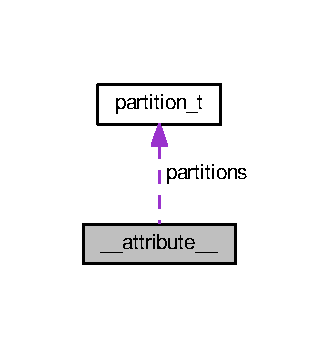
\includegraphics[width=160pt]{struct____attribute______coll__graph}
\end{center}
\end{figure}
\subsection*{Data Fields}
\begin{DoxyCompactItemize}
\item 
uint16\+\_\+t \hyperlink{struct____attribute_____aa0943b75cfebf20ce431adfbedf9f8c4}{flags}
\item 
uint16\+\_\+t \hyperlink{struct____attribute_____a8d815909cef8ca1b062a2ad96c660a9c}{unused1} \mbox{[}9\mbox{]}
\item 
char \hyperlink{struct____attribute_____af239f8158f86e02086ba58fd19b81da7}{serial} \mbox{[}20\mbox{]}
\item 
uint16\+\_\+t \hyperlink{struct____attribute_____a18f24001adf4149e889ed86a8cbaff54}{unused2} \mbox{[}3\mbox{]}
\item 
char \hyperlink{struct____attribute_____adad0e454dd0c9a6d03d0f4349e9453f8}{firmware} \mbox{[}8\mbox{]}
\item 
char \hyperlink{struct____attribute_____a0f032985bf7b712101efd1179aa4bf9f}{model} \mbox{[}40\mbox{]}
\item 
uint16\+\_\+t \hyperlink{struct____attribute_____a98a71d598e8fa28b0bec4f638bef0c4d}{sectors\+\_\+per\+\_\+int}
\item 
uint16\+\_\+t \hyperlink{struct____attribute_____a5e3c3ed46d04f2818d5d3edcf9b0300f}{unused3}
\item 
uint16\+\_\+t \hyperlink{struct____attribute_____a77a668765fcd25abfe5b7e5f4ee85108}{capabilities} \mbox{[}2\mbox{]}
\item 
uint16\+\_\+t \hyperlink{struct____attribute_____a0b098ce1ed9de8d4a04ebb0868821517}{unused4} \mbox{[}2\mbox{]}
\item 
uint16\+\_\+t \hyperlink{struct____attribute_____a97f810c4d498d2027968fc454a7f7edd}{valid\+\_\+ext\+\_\+data}
\item 
uint16\+\_\+t \hyperlink{struct____attribute_____a7ba552a7e1c4b9a14f34db29c9804f78}{unused5} \mbox{[}5\mbox{]}
\item 
uint16\+\_\+t \hyperlink{struct____attribute_____aff51436bd7bae12814f39dfdb34da0a9}{size\+\_\+of\+\_\+rw\+\_\+mult}
\item 
uint32\+\_\+t \hyperlink{struct____attribute_____a18dddf5fb27b047a1d7b9c0646d341dd}{sectors\+\_\+28}
\item 
uint16\+\_\+t \hyperlink{struct____attribute_____a2237e6caea302218050257b393aca1c8}{unused6} \mbox{[}38\mbox{]}
\item 
uint64\+\_\+t \hyperlink{struct____attribute_____ad9d8935f5c8aa639c75860621cbcaeef}{sectors\+\_\+48}
\item 
uint16\+\_\+t \hyperlink{struct____attribute_____a3ca12260c33c9b1431db806c9dcfe209}{unused7} \mbox{[}152\mbox{]}
\item 
uint8\+\_\+t \hyperlink{struct____attribute_____a91badd2352f9652b3d46be652188d843}{boostrap} \mbox{[}446\mbox{]}
\item 
\hyperlink{structpartition__t}{partition\+\_\+t} \hyperlink{struct____attribute_____aa806510421b3faee3fdc3de2dad5e822}{partitions} \mbox{[}4\mbox{]}
\item 
uint8\+\_\+t \hyperlink{struct____attribute_____aaee33b58b76a81f69b6f3c5bb225c571}{signature} \mbox{[}2\mbox{]}
\end{DoxyCompactItemize}


\subsection{Detailed Description}


Definition at line 199 of file ata.\+c.



\subsection{Field Documentation}
\index{\+\_\+\+\_\+attribute\+\_\+\+\_\+@{\+\_\+\+\_\+attribute\+\_\+\+\_\+}!boostrap@{boostrap}}
\index{boostrap@{boostrap}!\+\_\+\+\_\+attribute\+\_\+\+\_\+@{\+\_\+\+\_\+attribute\+\_\+\+\_\+}}
\subsubsection[{\texorpdfstring{boostrap}{boostrap}}]{\setlength{\rightskip}{0pt plus 5cm}uint8\+\_\+t \+\_\+\+\_\+attribute\+\_\+\+\_\+\+::boostrap\mbox{[}446\mbox{]}}\hypertarget{struct____attribute_____a91badd2352f9652b3d46be652188d843}{}\label{struct____attribute_____a91badd2352f9652b3d46be652188d843}


Definition at line 220 of file ata.\+c.

\index{\+\_\+\+\_\+attribute\+\_\+\+\_\+@{\+\_\+\+\_\+attribute\+\_\+\+\_\+}!capabilities@{capabilities}}
\index{capabilities@{capabilities}!\+\_\+\+\_\+attribute\+\_\+\+\_\+@{\+\_\+\+\_\+attribute\+\_\+\+\_\+}}
\subsubsection[{\texorpdfstring{capabilities}{capabilities}}]{\setlength{\rightskip}{0pt plus 5cm}uint16\+\_\+t \+\_\+\+\_\+attribute\+\_\+\+\_\+\+::capabilities\mbox{[}2\mbox{]}}\hypertarget{struct____attribute_____a77a668765fcd25abfe5b7e5f4ee85108}{}\label{struct____attribute_____a77a668765fcd25abfe5b7e5f4ee85108}


Definition at line 208 of file ata.\+c.

\index{\+\_\+\+\_\+attribute\+\_\+\+\_\+@{\+\_\+\+\_\+attribute\+\_\+\+\_\+}!firmware@{firmware}}
\index{firmware@{firmware}!\+\_\+\+\_\+attribute\+\_\+\+\_\+@{\+\_\+\+\_\+attribute\+\_\+\+\_\+}}
\subsubsection[{\texorpdfstring{firmware}{firmware}}]{\setlength{\rightskip}{0pt plus 5cm}char \+\_\+\+\_\+attribute\+\_\+\+\_\+\+::firmware\mbox{[}8\mbox{]}}\hypertarget{struct____attribute_____adad0e454dd0c9a6d03d0f4349e9453f8}{}\label{struct____attribute_____adad0e454dd0c9a6d03d0f4349e9453f8}


Definition at line 204 of file ata.\+c.

\index{\+\_\+\+\_\+attribute\+\_\+\+\_\+@{\+\_\+\+\_\+attribute\+\_\+\+\_\+}!flags@{flags}}
\index{flags@{flags}!\+\_\+\+\_\+attribute\+\_\+\+\_\+@{\+\_\+\+\_\+attribute\+\_\+\+\_\+}}
\subsubsection[{\texorpdfstring{flags}{flags}}]{\setlength{\rightskip}{0pt plus 5cm}uint16\+\_\+t \+\_\+\+\_\+attribute\+\_\+\+\_\+\+::flags}\hypertarget{struct____attribute_____aa0943b75cfebf20ce431adfbedf9f8c4}{}\label{struct____attribute_____aa0943b75cfebf20ce431adfbedf9f8c4}


Definition at line 200 of file ata.\+c.

\index{\+\_\+\+\_\+attribute\+\_\+\+\_\+@{\+\_\+\+\_\+attribute\+\_\+\+\_\+}!model@{model}}
\index{model@{model}!\+\_\+\+\_\+attribute\+\_\+\+\_\+@{\+\_\+\+\_\+attribute\+\_\+\+\_\+}}
\subsubsection[{\texorpdfstring{model}{model}}]{\setlength{\rightskip}{0pt plus 5cm}char \+\_\+\+\_\+attribute\+\_\+\+\_\+\+::model\mbox{[}40\mbox{]}}\hypertarget{struct____attribute_____a0f032985bf7b712101efd1179aa4bf9f}{}\label{struct____attribute_____a0f032985bf7b712101efd1179aa4bf9f}


Definition at line 205 of file ata.\+c.

\index{\+\_\+\+\_\+attribute\+\_\+\+\_\+@{\+\_\+\+\_\+attribute\+\_\+\+\_\+}!partitions@{partitions}}
\index{partitions@{partitions}!\+\_\+\+\_\+attribute\+\_\+\+\_\+@{\+\_\+\+\_\+attribute\+\_\+\+\_\+}}
\subsubsection[{\texorpdfstring{partitions}{partitions}}]{\setlength{\rightskip}{0pt plus 5cm}{\bf partition\+\_\+t} \+\_\+\+\_\+attribute\+\_\+\+\_\+\+::partitions\mbox{[}4\mbox{]}}\hypertarget{struct____attribute_____aa806510421b3faee3fdc3de2dad5e822}{}\label{struct____attribute_____aa806510421b3faee3fdc3de2dad5e822}


Definition at line 221 of file ata.\+c.

\index{\+\_\+\+\_\+attribute\+\_\+\+\_\+@{\+\_\+\+\_\+attribute\+\_\+\+\_\+}!sectors\+\_\+28@{sectors\+\_\+28}}
\index{sectors\+\_\+28@{sectors\+\_\+28}!\+\_\+\+\_\+attribute\+\_\+\+\_\+@{\+\_\+\+\_\+attribute\+\_\+\+\_\+}}
\subsubsection[{\texorpdfstring{sectors\+\_\+28}{sectors_28}}]{\setlength{\rightskip}{0pt plus 5cm}uint32\+\_\+t \+\_\+\+\_\+attribute\+\_\+\+\_\+\+::sectors\+\_\+28}\hypertarget{struct____attribute_____a18dddf5fb27b047a1d7b9c0646d341dd}{}\label{struct____attribute_____a18dddf5fb27b047a1d7b9c0646d341dd}


Definition at line 213 of file ata.\+c.

\index{\+\_\+\+\_\+attribute\+\_\+\+\_\+@{\+\_\+\+\_\+attribute\+\_\+\+\_\+}!sectors\+\_\+48@{sectors\+\_\+48}}
\index{sectors\+\_\+48@{sectors\+\_\+48}!\+\_\+\+\_\+attribute\+\_\+\+\_\+@{\+\_\+\+\_\+attribute\+\_\+\+\_\+}}
\subsubsection[{\texorpdfstring{sectors\+\_\+48}{sectors_48}}]{\setlength{\rightskip}{0pt plus 5cm}uint64\+\_\+t \+\_\+\+\_\+attribute\+\_\+\+\_\+\+::sectors\+\_\+48}\hypertarget{struct____attribute_____ad9d8935f5c8aa639c75860621cbcaeef}{}\label{struct____attribute_____ad9d8935f5c8aa639c75860621cbcaeef}


Definition at line 215 of file ata.\+c.

\index{\+\_\+\+\_\+attribute\+\_\+\+\_\+@{\+\_\+\+\_\+attribute\+\_\+\+\_\+}!sectors\+\_\+per\+\_\+int@{sectors\+\_\+per\+\_\+int}}
\index{sectors\+\_\+per\+\_\+int@{sectors\+\_\+per\+\_\+int}!\+\_\+\+\_\+attribute\+\_\+\+\_\+@{\+\_\+\+\_\+attribute\+\_\+\+\_\+}}
\subsubsection[{\texorpdfstring{sectors\+\_\+per\+\_\+int}{sectors_per_int}}]{\setlength{\rightskip}{0pt plus 5cm}uint16\+\_\+t \+\_\+\+\_\+attribute\+\_\+\+\_\+\+::sectors\+\_\+per\+\_\+int}\hypertarget{struct____attribute_____a98a71d598e8fa28b0bec4f638bef0c4d}{}\label{struct____attribute_____a98a71d598e8fa28b0bec4f638bef0c4d}


Definition at line 206 of file ata.\+c.

\index{\+\_\+\+\_\+attribute\+\_\+\+\_\+@{\+\_\+\+\_\+attribute\+\_\+\+\_\+}!serial@{serial}}
\index{serial@{serial}!\+\_\+\+\_\+attribute\+\_\+\+\_\+@{\+\_\+\+\_\+attribute\+\_\+\+\_\+}}
\subsubsection[{\texorpdfstring{serial}{serial}}]{\setlength{\rightskip}{0pt plus 5cm}char \+\_\+\+\_\+attribute\+\_\+\+\_\+\+::serial\mbox{[}20\mbox{]}}\hypertarget{struct____attribute_____af239f8158f86e02086ba58fd19b81da7}{}\label{struct____attribute_____af239f8158f86e02086ba58fd19b81da7}


Definition at line 202 of file ata.\+c.

\index{\+\_\+\+\_\+attribute\+\_\+\+\_\+@{\+\_\+\+\_\+attribute\+\_\+\+\_\+}!signature@{signature}}
\index{signature@{signature}!\+\_\+\+\_\+attribute\+\_\+\+\_\+@{\+\_\+\+\_\+attribute\+\_\+\+\_\+}}
\subsubsection[{\texorpdfstring{signature}{signature}}]{\setlength{\rightskip}{0pt plus 5cm}uint8\+\_\+t \+\_\+\+\_\+attribute\+\_\+\+\_\+\+::signature\mbox{[}2\mbox{]}}\hypertarget{struct____attribute_____aaee33b58b76a81f69b6f3c5bb225c571}{}\label{struct____attribute_____aaee33b58b76a81f69b6f3c5bb225c571}


Definition at line 222 of file ata.\+c.

\index{\+\_\+\+\_\+attribute\+\_\+\+\_\+@{\+\_\+\+\_\+attribute\+\_\+\+\_\+}!size\+\_\+of\+\_\+rw\+\_\+mult@{size\+\_\+of\+\_\+rw\+\_\+mult}}
\index{size\+\_\+of\+\_\+rw\+\_\+mult@{size\+\_\+of\+\_\+rw\+\_\+mult}!\+\_\+\+\_\+attribute\+\_\+\+\_\+@{\+\_\+\+\_\+attribute\+\_\+\+\_\+}}
\subsubsection[{\texorpdfstring{size\+\_\+of\+\_\+rw\+\_\+mult}{size_of_rw_mult}}]{\setlength{\rightskip}{0pt plus 5cm}uint16\+\_\+t \+\_\+\+\_\+attribute\+\_\+\+\_\+\+::size\+\_\+of\+\_\+rw\+\_\+mult}\hypertarget{struct____attribute_____aff51436bd7bae12814f39dfdb34da0a9}{}\label{struct____attribute_____aff51436bd7bae12814f39dfdb34da0a9}


Definition at line 212 of file ata.\+c.

\index{\+\_\+\+\_\+attribute\+\_\+\+\_\+@{\+\_\+\+\_\+attribute\+\_\+\+\_\+}!unused1@{unused1}}
\index{unused1@{unused1}!\+\_\+\+\_\+attribute\+\_\+\+\_\+@{\+\_\+\+\_\+attribute\+\_\+\+\_\+}}
\subsubsection[{\texorpdfstring{unused1}{unused1}}]{\setlength{\rightskip}{0pt plus 5cm}uint16\+\_\+t \+\_\+\+\_\+attribute\+\_\+\+\_\+\+::unused1\mbox{[}9\mbox{]}}\hypertarget{struct____attribute_____a8d815909cef8ca1b062a2ad96c660a9c}{}\label{struct____attribute_____a8d815909cef8ca1b062a2ad96c660a9c}


Definition at line 201 of file ata.\+c.

\index{\+\_\+\+\_\+attribute\+\_\+\+\_\+@{\+\_\+\+\_\+attribute\+\_\+\+\_\+}!unused2@{unused2}}
\index{unused2@{unused2}!\+\_\+\+\_\+attribute\+\_\+\+\_\+@{\+\_\+\+\_\+attribute\+\_\+\+\_\+}}
\subsubsection[{\texorpdfstring{unused2}{unused2}}]{\setlength{\rightskip}{0pt plus 5cm}uint16\+\_\+t \+\_\+\+\_\+attribute\+\_\+\+\_\+\+::unused2\mbox{[}3\mbox{]}}\hypertarget{struct____attribute_____a18f24001adf4149e889ed86a8cbaff54}{}\label{struct____attribute_____a18f24001adf4149e889ed86a8cbaff54}


Definition at line 203 of file ata.\+c.

\index{\+\_\+\+\_\+attribute\+\_\+\+\_\+@{\+\_\+\+\_\+attribute\+\_\+\+\_\+}!unused3@{unused3}}
\index{unused3@{unused3}!\+\_\+\+\_\+attribute\+\_\+\+\_\+@{\+\_\+\+\_\+attribute\+\_\+\+\_\+}}
\subsubsection[{\texorpdfstring{unused3}{unused3}}]{\setlength{\rightskip}{0pt plus 5cm}uint16\+\_\+t \+\_\+\+\_\+attribute\+\_\+\+\_\+\+::unused3}\hypertarget{struct____attribute_____a5e3c3ed46d04f2818d5d3edcf9b0300f}{}\label{struct____attribute_____a5e3c3ed46d04f2818d5d3edcf9b0300f}


Definition at line 207 of file ata.\+c.

\index{\+\_\+\+\_\+attribute\+\_\+\+\_\+@{\+\_\+\+\_\+attribute\+\_\+\+\_\+}!unused4@{unused4}}
\index{unused4@{unused4}!\+\_\+\+\_\+attribute\+\_\+\+\_\+@{\+\_\+\+\_\+attribute\+\_\+\+\_\+}}
\subsubsection[{\texorpdfstring{unused4}{unused4}}]{\setlength{\rightskip}{0pt plus 5cm}uint16\+\_\+t \+\_\+\+\_\+attribute\+\_\+\+\_\+\+::unused4\mbox{[}2\mbox{]}}\hypertarget{struct____attribute_____a0b098ce1ed9de8d4a04ebb0868821517}{}\label{struct____attribute_____a0b098ce1ed9de8d4a04ebb0868821517}


Definition at line 209 of file ata.\+c.

\index{\+\_\+\+\_\+attribute\+\_\+\+\_\+@{\+\_\+\+\_\+attribute\+\_\+\+\_\+}!unused5@{unused5}}
\index{unused5@{unused5}!\+\_\+\+\_\+attribute\+\_\+\+\_\+@{\+\_\+\+\_\+attribute\+\_\+\+\_\+}}
\subsubsection[{\texorpdfstring{unused5}{unused5}}]{\setlength{\rightskip}{0pt plus 5cm}uint16\+\_\+t \+\_\+\+\_\+attribute\+\_\+\+\_\+\+::unused5\mbox{[}5\mbox{]}}\hypertarget{struct____attribute_____a7ba552a7e1c4b9a14f34db29c9804f78}{}\label{struct____attribute_____a7ba552a7e1c4b9a14f34db29c9804f78}


Definition at line 211 of file ata.\+c.

\index{\+\_\+\+\_\+attribute\+\_\+\+\_\+@{\+\_\+\+\_\+attribute\+\_\+\+\_\+}!unused6@{unused6}}
\index{unused6@{unused6}!\+\_\+\+\_\+attribute\+\_\+\+\_\+@{\+\_\+\+\_\+attribute\+\_\+\+\_\+}}
\subsubsection[{\texorpdfstring{unused6}{unused6}}]{\setlength{\rightskip}{0pt plus 5cm}uint16\+\_\+t \+\_\+\+\_\+attribute\+\_\+\+\_\+\+::unused6\mbox{[}38\mbox{]}}\hypertarget{struct____attribute_____a2237e6caea302218050257b393aca1c8}{}\label{struct____attribute_____a2237e6caea302218050257b393aca1c8}


Definition at line 214 of file ata.\+c.

\index{\+\_\+\+\_\+attribute\+\_\+\+\_\+@{\+\_\+\+\_\+attribute\+\_\+\+\_\+}!unused7@{unused7}}
\index{unused7@{unused7}!\+\_\+\+\_\+attribute\+\_\+\+\_\+@{\+\_\+\+\_\+attribute\+\_\+\+\_\+}}
\subsubsection[{\texorpdfstring{unused7}{unused7}}]{\setlength{\rightskip}{0pt plus 5cm}uint16\+\_\+t \+\_\+\+\_\+attribute\+\_\+\+\_\+\+::unused7\mbox{[}152\mbox{]}}\hypertarget{struct____attribute_____a3ca12260c33c9b1431db806c9dcfe209}{}\label{struct____attribute_____a3ca12260c33c9b1431db806c9dcfe209}


Definition at line 216 of file ata.\+c.

\index{\+\_\+\+\_\+attribute\+\_\+\+\_\+@{\+\_\+\+\_\+attribute\+\_\+\+\_\+}!valid\+\_\+ext\+\_\+data@{valid\+\_\+ext\+\_\+data}}
\index{valid\+\_\+ext\+\_\+data@{valid\+\_\+ext\+\_\+data}!\+\_\+\+\_\+attribute\+\_\+\+\_\+@{\+\_\+\+\_\+attribute\+\_\+\+\_\+}}
\subsubsection[{\texorpdfstring{valid\+\_\+ext\+\_\+data}{valid_ext_data}}]{\setlength{\rightskip}{0pt plus 5cm}uint16\+\_\+t \+\_\+\+\_\+attribute\+\_\+\+\_\+\+::valid\+\_\+ext\+\_\+data}\hypertarget{struct____attribute_____a97f810c4d498d2027968fc454a7f7edd}{}\label{struct____attribute_____a97f810c4d498d2027968fc454a7f7edd}


Definition at line 210 of file ata.\+c.



The documentation for this struct was generated from the following file\+:\begin{DoxyCompactItemize}
\item 
Experimental Edition/\+Source/\+Drivers/\+A\+T\+A/\hyperlink{ata_8c}{ata.\+c}\end{DoxyCompactItemize}

\hypertarget{struct____tss__struct}{}\section{\+\_\+\+\_\+tss\+\_\+struct Struct Reference}
\label{struct____tss__struct}\index{\+\_\+\+\_\+tss\+\_\+struct@{\+\_\+\+\_\+tss\+\_\+struct}}


{\ttfamily \#include $<$task.\+h$>$}

\subsection*{Data Fields}
\begin{DoxyCompactItemize}
\item 
unsigned short \hyperlink{struct____tss__struct_ae95a2fc5b42ac4b190cb4c340dfe0ab2}{link}
\item 
unsigned short \hyperlink{struct____tss__struct_a09d41cf0b65451fe0238b32ae9797bf0}{link\+\_\+h}
\item 
unsigned long \hyperlink{struct____tss__struct_a7d2c471a5e5070e75f2b11c70fa3374c}{esp0}
\item 
unsigned short \hyperlink{struct____tss__struct_a64d13cf91ec122ec8ed42917b9dd471b}{ss0}
\item 
unsigned short \hyperlink{struct____tss__struct_a06f3d0a7a04074ed8772d8ee810c9a38}{ss0\+\_\+h}
\item 
unsigned long \hyperlink{struct____tss__struct_a0c8844d2b2cd289b6d8b91cb37089592}{esp1}
\item 
unsigned short \hyperlink{struct____tss__struct_a1c405de895c4eb4ffe2930361aa252d3}{ss1}
\item 
unsigned short \hyperlink{struct____tss__struct_a3bbb779909ca09f2003bf80d78f62cbe}{ss1\+\_\+h}
\item 
unsigned long \hyperlink{struct____tss__struct_aae8e9f58e67ba8b83b7d9876885ff68b}{esp2}
\item 
unsigned short \hyperlink{struct____tss__struct_a38e2e31267942cf914f1f87e95e06152}{ss2}
\item 
unsigned short \hyperlink{struct____tss__struct_adef7bc907c882bdf83a27b682583f9cd}{ss2\+\_\+h}
\item 
unsigned long \hyperlink{struct____tss__struct_afd7f71893266af35fef0279fb2f9af42}{cr3}
\item 
unsigned long \hyperlink{struct____tss__struct_a5405817bf20081bfbd4007f146e787bd}{eip}
\item 
unsigned long \hyperlink{struct____tss__struct_ad0b672eea10bdec2d43cfee9f1ca5c4c}{eflags}
\item 
unsigned long \hyperlink{struct____tss__struct_aa70f529f7adea9e30313ef9fcd0191da}{eax}
\item 
unsigned long \hyperlink{struct____tss__struct_ab0e3aa7395c5639c49855a2dd5cc2be0}{ecx}
\item 
unsigned long \hyperlink{struct____tss__struct_affcb93ba4eb271762b3167a13be06a83}{edx}
\item 
unsigned long \hyperlink{struct____tss__struct_ac67f49c13b208df1720f9ca9c0da17dc}{ebx}
\item 
unsigned long \hyperlink{struct____tss__struct_aa35a140c36667e429be9f52526e5c019}{esp}
\item 
unsigned long \hyperlink{struct____tss__struct_abe00097e1842c728d70854ca727da16c}{ebp}
\item 
unsigned long \hyperlink{struct____tss__struct_aa726c858975c07c9f225dfb1143fa638}{esi}
\item 
unsigned long \hyperlink{struct____tss__struct_a3f7cde8faad6aa59cd3b36bf8493a315}{edi}
\item 
unsigned short \hyperlink{struct____tss__struct_a068c08e101d0fd8e66cb315446f64532}{es}
\item 
unsigned short \hyperlink{struct____tss__struct_a2578c9748d5a0bd005dead21a80bd5e5}{es\+\_\+h}
\item 
unsigned short \hyperlink{struct____tss__struct_adbf2980b4b9a4b505dbb3886ad657357}{cs}
\item 
unsigned short \hyperlink{struct____tss__struct_a20fd7d98f390bda555de791fff0d6fda}{cs\+\_\+h}
\item 
unsigned short \hyperlink{struct____tss__struct_abc595ca5102923b8b55bb4ce98bbe8db}{ss}
\item 
unsigned short \hyperlink{struct____tss__struct_a1c717fd639092811a9d4b548d6115b36}{ss\+\_\+h}
\item 
unsigned short \hyperlink{struct____tss__struct_a7d135efa48729e8d72c58f68395d0a23}{ds}
\item 
unsigned short \hyperlink{struct____tss__struct_a21e478f52a03d836cc45af1a49f4d876}{ds\+\_\+h}
\item 
unsigned short \hyperlink{struct____tss__struct_a4f47bf398ce57037b89c3b9f42e0ce18}{fs}
\item 
unsigned short \hyperlink{struct____tss__struct_a065694d5def8420fa4411053c460cb04}{fs\+\_\+h}
\item 
unsigned short \hyperlink{struct____tss__struct_ad99e75893aedb89cd0e136e3e6e57727}{gs}
\item 
unsigned short \hyperlink{struct____tss__struct_a724b8bddadd1b77d08b16d4292f3ac77}{gs\+\_\+h}
\item 
unsigned short \hyperlink{struct____tss__struct_a16d41b1184cf4d1a2af29cd288635c78}{ldt}
\item 
unsigned short \hyperlink{struct____tss__struct_a8b926ac70ecae62767750d002da4112e}{ldt\+\_\+h}
\item 
unsigned short \hyperlink{struct____tss__struct_a1bb5da85377e5612cddb13b0ac403e4e}{trap}
\item 
unsigned short \hyperlink{struct____tss__struct_a2ee32c201d129f8ee19dfd510b5d69fd}{iomap}
\end{DoxyCompactItemize}


\subsection{Detailed Description}


Definition at line 61 of file task.\+h.



\subsection{Field Documentation}
\index{\+\_\+\+\_\+tss\+\_\+struct@{\+\_\+\+\_\+tss\+\_\+struct}!cr3@{cr3}}
\index{cr3@{cr3}!\+\_\+\+\_\+tss\+\_\+struct@{\+\_\+\+\_\+tss\+\_\+struct}}
\subsubsection[{\texorpdfstring{cr3}{cr3}}]{\setlength{\rightskip}{0pt plus 5cm}unsigned long \+\_\+\+\_\+tss\+\_\+struct\+::cr3}\hypertarget{struct____tss__struct_afd7f71893266af35fef0279fb2f9af42}{}\label{struct____tss__struct_afd7f71893266af35fef0279fb2f9af42}


Definition at line 78 of file task.\+h.

\index{\+\_\+\+\_\+tss\+\_\+struct@{\+\_\+\+\_\+tss\+\_\+struct}!cs@{cs}}
\index{cs@{cs}!\+\_\+\+\_\+tss\+\_\+struct@{\+\_\+\+\_\+tss\+\_\+struct}}
\subsubsection[{\texorpdfstring{cs}{cs}}]{\setlength{\rightskip}{0pt plus 5cm}unsigned short \+\_\+\+\_\+tss\+\_\+struct\+::cs}\hypertarget{struct____tss__struct_adbf2980b4b9a4b505dbb3886ad657357}{}\label{struct____tss__struct_adbf2980b4b9a4b505dbb3886ad657357}


Definition at line 96 of file task.\+h.

\index{\+\_\+\+\_\+tss\+\_\+struct@{\+\_\+\+\_\+tss\+\_\+struct}!cs\+\_\+h@{cs\+\_\+h}}
\index{cs\+\_\+h@{cs\+\_\+h}!\+\_\+\+\_\+tss\+\_\+struct@{\+\_\+\+\_\+tss\+\_\+struct}}
\subsubsection[{\texorpdfstring{cs\+\_\+h}{cs_h}}]{\setlength{\rightskip}{0pt plus 5cm}unsigned short \+\_\+\+\_\+tss\+\_\+struct\+::cs\+\_\+h}\hypertarget{struct____tss__struct_a20fd7d98f390bda555de791fff0d6fda}{}\label{struct____tss__struct_a20fd7d98f390bda555de791fff0d6fda}


Definition at line 97 of file task.\+h.

\index{\+\_\+\+\_\+tss\+\_\+struct@{\+\_\+\+\_\+tss\+\_\+struct}!ds@{ds}}
\index{ds@{ds}!\+\_\+\+\_\+tss\+\_\+struct@{\+\_\+\+\_\+tss\+\_\+struct}}
\subsubsection[{\texorpdfstring{ds}{ds}}]{\setlength{\rightskip}{0pt plus 5cm}unsigned short \+\_\+\+\_\+tss\+\_\+struct\+::ds}\hypertarget{struct____tss__struct_a7d135efa48729e8d72c58f68395d0a23}{}\label{struct____tss__struct_a7d135efa48729e8d72c58f68395d0a23}


Definition at line 102 of file task.\+h.

\index{\+\_\+\+\_\+tss\+\_\+struct@{\+\_\+\+\_\+tss\+\_\+struct}!ds\+\_\+h@{ds\+\_\+h}}
\index{ds\+\_\+h@{ds\+\_\+h}!\+\_\+\+\_\+tss\+\_\+struct@{\+\_\+\+\_\+tss\+\_\+struct}}
\subsubsection[{\texorpdfstring{ds\+\_\+h}{ds_h}}]{\setlength{\rightskip}{0pt plus 5cm}unsigned short \+\_\+\+\_\+tss\+\_\+struct\+::ds\+\_\+h}\hypertarget{struct____tss__struct_a21e478f52a03d836cc45af1a49f4d876}{}\label{struct____tss__struct_a21e478f52a03d836cc45af1a49f4d876}


Definition at line 103 of file task.\+h.

\index{\+\_\+\+\_\+tss\+\_\+struct@{\+\_\+\+\_\+tss\+\_\+struct}!eax@{eax}}
\index{eax@{eax}!\+\_\+\+\_\+tss\+\_\+struct@{\+\_\+\+\_\+tss\+\_\+struct}}
\subsubsection[{\texorpdfstring{eax}{eax}}]{\setlength{\rightskip}{0pt plus 5cm}unsigned long \+\_\+\+\_\+tss\+\_\+struct\+::eax}\hypertarget{struct____tss__struct_aa70f529f7adea9e30313ef9fcd0191da}{}\label{struct____tss__struct_aa70f529f7adea9e30313ef9fcd0191da}


Definition at line 82 of file task.\+h.

\index{\+\_\+\+\_\+tss\+\_\+struct@{\+\_\+\+\_\+tss\+\_\+struct}!ebp@{ebp}}
\index{ebp@{ebp}!\+\_\+\+\_\+tss\+\_\+struct@{\+\_\+\+\_\+tss\+\_\+struct}}
\subsubsection[{\texorpdfstring{ebp}{ebp}}]{\setlength{\rightskip}{0pt plus 5cm}unsigned long \+\_\+\+\_\+tss\+\_\+struct\+::ebp}\hypertarget{struct____tss__struct_abe00097e1842c728d70854ca727da16c}{}\label{struct____tss__struct_abe00097e1842c728d70854ca727da16c}


Definition at line 88 of file task.\+h.

\index{\+\_\+\+\_\+tss\+\_\+struct@{\+\_\+\+\_\+tss\+\_\+struct}!ebx@{ebx}}
\index{ebx@{ebx}!\+\_\+\+\_\+tss\+\_\+struct@{\+\_\+\+\_\+tss\+\_\+struct}}
\subsubsection[{\texorpdfstring{ebx}{ebx}}]{\setlength{\rightskip}{0pt plus 5cm}unsigned long \+\_\+\+\_\+tss\+\_\+struct\+::ebx}\hypertarget{struct____tss__struct_ac67f49c13b208df1720f9ca9c0da17dc}{}\label{struct____tss__struct_ac67f49c13b208df1720f9ca9c0da17dc}


Definition at line 85 of file task.\+h.

\index{\+\_\+\+\_\+tss\+\_\+struct@{\+\_\+\+\_\+tss\+\_\+struct}!ecx@{ecx}}
\index{ecx@{ecx}!\+\_\+\+\_\+tss\+\_\+struct@{\+\_\+\+\_\+tss\+\_\+struct}}
\subsubsection[{\texorpdfstring{ecx}{ecx}}]{\setlength{\rightskip}{0pt plus 5cm}unsigned long \+\_\+\+\_\+tss\+\_\+struct\+::ecx}\hypertarget{struct____tss__struct_ab0e3aa7395c5639c49855a2dd5cc2be0}{}\label{struct____tss__struct_ab0e3aa7395c5639c49855a2dd5cc2be0}


Definition at line 83 of file task.\+h.

\index{\+\_\+\+\_\+tss\+\_\+struct@{\+\_\+\+\_\+tss\+\_\+struct}!edi@{edi}}
\index{edi@{edi}!\+\_\+\+\_\+tss\+\_\+struct@{\+\_\+\+\_\+tss\+\_\+struct}}
\subsubsection[{\texorpdfstring{edi}{edi}}]{\setlength{\rightskip}{0pt plus 5cm}unsigned long \+\_\+\+\_\+tss\+\_\+struct\+::edi}\hypertarget{struct____tss__struct_a3f7cde8faad6aa59cd3b36bf8493a315}{}\label{struct____tss__struct_a3f7cde8faad6aa59cd3b36bf8493a315}


Definition at line 91 of file task.\+h.

\index{\+\_\+\+\_\+tss\+\_\+struct@{\+\_\+\+\_\+tss\+\_\+struct}!edx@{edx}}
\index{edx@{edx}!\+\_\+\+\_\+tss\+\_\+struct@{\+\_\+\+\_\+tss\+\_\+struct}}
\subsubsection[{\texorpdfstring{edx}{edx}}]{\setlength{\rightskip}{0pt plus 5cm}unsigned long \+\_\+\+\_\+tss\+\_\+struct\+::edx}\hypertarget{struct____tss__struct_affcb93ba4eb271762b3167a13be06a83}{}\label{struct____tss__struct_affcb93ba4eb271762b3167a13be06a83}


Definition at line 84 of file task.\+h.

\index{\+\_\+\+\_\+tss\+\_\+struct@{\+\_\+\+\_\+tss\+\_\+struct}!eflags@{eflags}}
\index{eflags@{eflags}!\+\_\+\+\_\+tss\+\_\+struct@{\+\_\+\+\_\+tss\+\_\+struct}}
\subsubsection[{\texorpdfstring{eflags}{eflags}}]{\setlength{\rightskip}{0pt plus 5cm}unsigned long \+\_\+\+\_\+tss\+\_\+struct\+::eflags}\hypertarget{struct____tss__struct_ad0b672eea10bdec2d43cfee9f1ca5c4c}{}\label{struct____tss__struct_ad0b672eea10bdec2d43cfee9f1ca5c4c}


Definition at line 80 of file task.\+h.

\index{\+\_\+\+\_\+tss\+\_\+struct@{\+\_\+\+\_\+tss\+\_\+struct}!eip@{eip}}
\index{eip@{eip}!\+\_\+\+\_\+tss\+\_\+struct@{\+\_\+\+\_\+tss\+\_\+struct}}
\subsubsection[{\texorpdfstring{eip}{eip}}]{\setlength{\rightskip}{0pt plus 5cm}unsigned long \+\_\+\+\_\+tss\+\_\+struct\+::eip}\hypertarget{struct____tss__struct_a5405817bf20081bfbd4007f146e787bd}{}\label{struct____tss__struct_a5405817bf20081bfbd4007f146e787bd}


Definition at line 79 of file task.\+h.

\index{\+\_\+\+\_\+tss\+\_\+struct@{\+\_\+\+\_\+tss\+\_\+struct}!es@{es}}
\index{es@{es}!\+\_\+\+\_\+tss\+\_\+struct@{\+\_\+\+\_\+tss\+\_\+struct}}
\subsubsection[{\texorpdfstring{es}{es}}]{\setlength{\rightskip}{0pt plus 5cm}unsigned short \+\_\+\+\_\+tss\+\_\+struct\+::es}\hypertarget{struct____tss__struct_a068c08e101d0fd8e66cb315446f64532}{}\label{struct____tss__struct_a068c08e101d0fd8e66cb315446f64532}


Definition at line 93 of file task.\+h.

\index{\+\_\+\+\_\+tss\+\_\+struct@{\+\_\+\+\_\+tss\+\_\+struct}!es\+\_\+h@{es\+\_\+h}}
\index{es\+\_\+h@{es\+\_\+h}!\+\_\+\+\_\+tss\+\_\+struct@{\+\_\+\+\_\+tss\+\_\+struct}}
\subsubsection[{\texorpdfstring{es\+\_\+h}{es_h}}]{\setlength{\rightskip}{0pt plus 5cm}unsigned short \+\_\+\+\_\+tss\+\_\+struct\+::es\+\_\+h}\hypertarget{struct____tss__struct_a2578c9748d5a0bd005dead21a80bd5e5}{}\label{struct____tss__struct_a2578c9748d5a0bd005dead21a80bd5e5}


Definition at line 94 of file task.\+h.

\index{\+\_\+\+\_\+tss\+\_\+struct@{\+\_\+\+\_\+tss\+\_\+struct}!esi@{esi}}
\index{esi@{esi}!\+\_\+\+\_\+tss\+\_\+struct@{\+\_\+\+\_\+tss\+\_\+struct}}
\subsubsection[{\texorpdfstring{esi}{esi}}]{\setlength{\rightskip}{0pt plus 5cm}unsigned long \+\_\+\+\_\+tss\+\_\+struct\+::esi}\hypertarget{struct____tss__struct_aa726c858975c07c9f225dfb1143fa638}{}\label{struct____tss__struct_aa726c858975c07c9f225dfb1143fa638}


Definition at line 90 of file task.\+h.

\index{\+\_\+\+\_\+tss\+\_\+struct@{\+\_\+\+\_\+tss\+\_\+struct}!esp@{esp}}
\index{esp@{esp}!\+\_\+\+\_\+tss\+\_\+struct@{\+\_\+\+\_\+tss\+\_\+struct}}
\subsubsection[{\texorpdfstring{esp}{esp}}]{\setlength{\rightskip}{0pt plus 5cm}unsigned long \+\_\+\+\_\+tss\+\_\+struct\+::esp}\hypertarget{struct____tss__struct_aa35a140c36667e429be9f52526e5c019}{}\label{struct____tss__struct_aa35a140c36667e429be9f52526e5c019}


Definition at line 87 of file task.\+h.

\index{\+\_\+\+\_\+tss\+\_\+struct@{\+\_\+\+\_\+tss\+\_\+struct}!esp0@{esp0}}
\index{esp0@{esp0}!\+\_\+\+\_\+tss\+\_\+struct@{\+\_\+\+\_\+tss\+\_\+struct}}
\subsubsection[{\texorpdfstring{esp0}{esp0}}]{\setlength{\rightskip}{0pt plus 5cm}unsigned long \+\_\+\+\_\+tss\+\_\+struct\+::esp0}\hypertarget{struct____tss__struct_a7d2c471a5e5070e75f2b11c70fa3374c}{}\label{struct____tss__struct_a7d2c471a5e5070e75f2b11c70fa3374c}


Definition at line 66 of file task.\+h.

\index{\+\_\+\+\_\+tss\+\_\+struct@{\+\_\+\+\_\+tss\+\_\+struct}!esp1@{esp1}}
\index{esp1@{esp1}!\+\_\+\+\_\+tss\+\_\+struct@{\+\_\+\+\_\+tss\+\_\+struct}}
\subsubsection[{\texorpdfstring{esp1}{esp1}}]{\setlength{\rightskip}{0pt plus 5cm}unsigned long \+\_\+\+\_\+tss\+\_\+struct\+::esp1}\hypertarget{struct____tss__struct_a0c8844d2b2cd289b6d8b91cb37089592}{}\label{struct____tss__struct_a0c8844d2b2cd289b6d8b91cb37089592}


Definition at line 70 of file task.\+h.

\index{\+\_\+\+\_\+tss\+\_\+struct@{\+\_\+\+\_\+tss\+\_\+struct}!esp2@{esp2}}
\index{esp2@{esp2}!\+\_\+\+\_\+tss\+\_\+struct@{\+\_\+\+\_\+tss\+\_\+struct}}
\subsubsection[{\texorpdfstring{esp2}{esp2}}]{\setlength{\rightskip}{0pt plus 5cm}unsigned long \+\_\+\+\_\+tss\+\_\+struct\+::esp2}\hypertarget{struct____tss__struct_aae8e9f58e67ba8b83b7d9876885ff68b}{}\label{struct____tss__struct_aae8e9f58e67ba8b83b7d9876885ff68b}


Definition at line 74 of file task.\+h.

\index{\+\_\+\+\_\+tss\+\_\+struct@{\+\_\+\+\_\+tss\+\_\+struct}!fs@{fs}}
\index{fs@{fs}!\+\_\+\+\_\+tss\+\_\+struct@{\+\_\+\+\_\+tss\+\_\+struct}}
\subsubsection[{\texorpdfstring{fs}{fs}}]{\setlength{\rightskip}{0pt plus 5cm}unsigned short \+\_\+\+\_\+tss\+\_\+struct\+::fs}\hypertarget{struct____tss__struct_a4f47bf398ce57037b89c3b9f42e0ce18}{}\label{struct____tss__struct_a4f47bf398ce57037b89c3b9f42e0ce18}


Definition at line 105 of file task.\+h.

\index{\+\_\+\+\_\+tss\+\_\+struct@{\+\_\+\+\_\+tss\+\_\+struct}!fs\+\_\+h@{fs\+\_\+h}}
\index{fs\+\_\+h@{fs\+\_\+h}!\+\_\+\+\_\+tss\+\_\+struct@{\+\_\+\+\_\+tss\+\_\+struct}}
\subsubsection[{\texorpdfstring{fs\+\_\+h}{fs_h}}]{\setlength{\rightskip}{0pt plus 5cm}unsigned short \+\_\+\+\_\+tss\+\_\+struct\+::fs\+\_\+h}\hypertarget{struct____tss__struct_a065694d5def8420fa4411053c460cb04}{}\label{struct____tss__struct_a065694d5def8420fa4411053c460cb04}


Definition at line 106 of file task.\+h.

\index{\+\_\+\+\_\+tss\+\_\+struct@{\+\_\+\+\_\+tss\+\_\+struct}!gs@{gs}}
\index{gs@{gs}!\+\_\+\+\_\+tss\+\_\+struct@{\+\_\+\+\_\+tss\+\_\+struct}}
\subsubsection[{\texorpdfstring{gs}{gs}}]{\setlength{\rightskip}{0pt plus 5cm}unsigned short \+\_\+\+\_\+tss\+\_\+struct\+::gs}\hypertarget{struct____tss__struct_ad99e75893aedb89cd0e136e3e6e57727}{}\label{struct____tss__struct_ad99e75893aedb89cd0e136e3e6e57727}


Definition at line 108 of file task.\+h.

\index{\+\_\+\+\_\+tss\+\_\+struct@{\+\_\+\+\_\+tss\+\_\+struct}!gs\+\_\+h@{gs\+\_\+h}}
\index{gs\+\_\+h@{gs\+\_\+h}!\+\_\+\+\_\+tss\+\_\+struct@{\+\_\+\+\_\+tss\+\_\+struct}}
\subsubsection[{\texorpdfstring{gs\+\_\+h}{gs_h}}]{\setlength{\rightskip}{0pt plus 5cm}unsigned short \+\_\+\+\_\+tss\+\_\+struct\+::gs\+\_\+h}\hypertarget{struct____tss__struct_a724b8bddadd1b77d08b16d4292f3ac77}{}\label{struct____tss__struct_a724b8bddadd1b77d08b16d4292f3ac77}


Definition at line 109 of file task.\+h.

\index{\+\_\+\+\_\+tss\+\_\+struct@{\+\_\+\+\_\+tss\+\_\+struct}!iomap@{iomap}}
\index{iomap@{iomap}!\+\_\+\+\_\+tss\+\_\+struct@{\+\_\+\+\_\+tss\+\_\+struct}}
\subsubsection[{\texorpdfstring{iomap}{iomap}}]{\setlength{\rightskip}{0pt plus 5cm}unsigned short \+\_\+\+\_\+tss\+\_\+struct\+::iomap}\hypertarget{struct____tss__struct_a2ee32c201d129f8ee19dfd510b5d69fd}{}\label{struct____tss__struct_a2ee32c201d129f8ee19dfd510b5d69fd}


Definition at line 115 of file task.\+h.

\index{\+\_\+\+\_\+tss\+\_\+struct@{\+\_\+\+\_\+tss\+\_\+struct}!ldt@{ldt}}
\index{ldt@{ldt}!\+\_\+\+\_\+tss\+\_\+struct@{\+\_\+\+\_\+tss\+\_\+struct}}
\subsubsection[{\texorpdfstring{ldt}{ldt}}]{\setlength{\rightskip}{0pt plus 5cm}unsigned short \+\_\+\+\_\+tss\+\_\+struct\+::ldt}\hypertarget{struct____tss__struct_a16d41b1184cf4d1a2af29cd288635c78}{}\label{struct____tss__struct_a16d41b1184cf4d1a2af29cd288635c78}


Definition at line 111 of file task.\+h.

\index{\+\_\+\+\_\+tss\+\_\+struct@{\+\_\+\+\_\+tss\+\_\+struct}!ldt\+\_\+h@{ldt\+\_\+h}}
\index{ldt\+\_\+h@{ldt\+\_\+h}!\+\_\+\+\_\+tss\+\_\+struct@{\+\_\+\+\_\+tss\+\_\+struct}}
\subsubsection[{\texorpdfstring{ldt\+\_\+h}{ldt_h}}]{\setlength{\rightskip}{0pt plus 5cm}unsigned short \+\_\+\+\_\+tss\+\_\+struct\+::ldt\+\_\+h}\hypertarget{struct____tss__struct_a8b926ac70ecae62767750d002da4112e}{}\label{struct____tss__struct_a8b926ac70ecae62767750d002da4112e}


Definition at line 112 of file task.\+h.

\index{\+\_\+\+\_\+tss\+\_\+struct@{\+\_\+\+\_\+tss\+\_\+struct}!link@{link}}
\index{link@{link}!\+\_\+\+\_\+tss\+\_\+struct@{\+\_\+\+\_\+tss\+\_\+struct}}
\subsubsection[{\texorpdfstring{link}{link}}]{\setlength{\rightskip}{0pt plus 5cm}unsigned short \+\_\+\+\_\+tss\+\_\+struct\+::link}\hypertarget{struct____tss__struct_ae95a2fc5b42ac4b190cb4c340dfe0ab2}{}\label{struct____tss__struct_ae95a2fc5b42ac4b190cb4c340dfe0ab2}


Definition at line 63 of file task.\+h.

\index{\+\_\+\+\_\+tss\+\_\+struct@{\+\_\+\+\_\+tss\+\_\+struct}!link\+\_\+h@{link\+\_\+h}}
\index{link\+\_\+h@{link\+\_\+h}!\+\_\+\+\_\+tss\+\_\+struct@{\+\_\+\+\_\+tss\+\_\+struct}}
\subsubsection[{\texorpdfstring{link\+\_\+h}{link_h}}]{\setlength{\rightskip}{0pt plus 5cm}unsigned short \+\_\+\+\_\+tss\+\_\+struct\+::link\+\_\+h}\hypertarget{struct____tss__struct_a09d41cf0b65451fe0238b32ae9797bf0}{}\label{struct____tss__struct_a09d41cf0b65451fe0238b32ae9797bf0}


Definition at line 64 of file task.\+h.

\index{\+\_\+\+\_\+tss\+\_\+struct@{\+\_\+\+\_\+tss\+\_\+struct}!ss@{ss}}
\index{ss@{ss}!\+\_\+\+\_\+tss\+\_\+struct@{\+\_\+\+\_\+tss\+\_\+struct}}
\subsubsection[{\texorpdfstring{ss}{ss}}]{\setlength{\rightskip}{0pt plus 5cm}unsigned short \+\_\+\+\_\+tss\+\_\+struct\+::ss}\hypertarget{struct____tss__struct_abc595ca5102923b8b55bb4ce98bbe8db}{}\label{struct____tss__struct_abc595ca5102923b8b55bb4ce98bbe8db}


Definition at line 99 of file task.\+h.

\index{\+\_\+\+\_\+tss\+\_\+struct@{\+\_\+\+\_\+tss\+\_\+struct}!ss0@{ss0}}
\index{ss0@{ss0}!\+\_\+\+\_\+tss\+\_\+struct@{\+\_\+\+\_\+tss\+\_\+struct}}
\subsubsection[{\texorpdfstring{ss0}{ss0}}]{\setlength{\rightskip}{0pt plus 5cm}unsigned short \+\_\+\+\_\+tss\+\_\+struct\+::ss0}\hypertarget{struct____tss__struct_a64d13cf91ec122ec8ed42917b9dd471b}{}\label{struct____tss__struct_a64d13cf91ec122ec8ed42917b9dd471b}


Definition at line 67 of file task.\+h.

\index{\+\_\+\+\_\+tss\+\_\+struct@{\+\_\+\+\_\+tss\+\_\+struct}!ss0\+\_\+h@{ss0\+\_\+h}}
\index{ss0\+\_\+h@{ss0\+\_\+h}!\+\_\+\+\_\+tss\+\_\+struct@{\+\_\+\+\_\+tss\+\_\+struct}}
\subsubsection[{\texorpdfstring{ss0\+\_\+h}{ss0_h}}]{\setlength{\rightskip}{0pt plus 5cm}unsigned short \+\_\+\+\_\+tss\+\_\+struct\+::ss0\+\_\+h}\hypertarget{struct____tss__struct_a06f3d0a7a04074ed8772d8ee810c9a38}{}\label{struct____tss__struct_a06f3d0a7a04074ed8772d8ee810c9a38}


Definition at line 68 of file task.\+h.

\index{\+\_\+\+\_\+tss\+\_\+struct@{\+\_\+\+\_\+tss\+\_\+struct}!ss1@{ss1}}
\index{ss1@{ss1}!\+\_\+\+\_\+tss\+\_\+struct@{\+\_\+\+\_\+tss\+\_\+struct}}
\subsubsection[{\texorpdfstring{ss1}{ss1}}]{\setlength{\rightskip}{0pt plus 5cm}unsigned short \+\_\+\+\_\+tss\+\_\+struct\+::ss1}\hypertarget{struct____tss__struct_a1c405de895c4eb4ffe2930361aa252d3}{}\label{struct____tss__struct_a1c405de895c4eb4ffe2930361aa252d3}


Definition at line 71 of file task.\+h.

\index{\+\_\+\+\_\+tss\+\_\+struct@{\+\_\+\+\_\+tss\+\_\+struct}!ss1\+\_\+h@{ss1\+\_\+h}}
\index{ss1\+\_\+h@{ss1\+\_\+h}!\+\_\+\+\_\+tss\+\_\+struct@{\+\_\+\+\_\+tss\+\_\+struct}}
\subsubsection[{\texorpdfstring{ss1\+\_\+h}{ss1_h}}]{\setlength{\rightskip}{0pt plus 5cm}unsigned short \+\_\+\+\_\+tss\+\_\+struct\+::ss1\+\_\+h}\hypertarget{struct____tss__struct_a3bbb779909ca09f2003bf80d78f62cbe}{}\label{struct____tss__struct_a3bbb779909ca09f2003bf80d78f62cbe}


Definition at line 72 of file task.\+h.

\index{\+\_\+\+\_\+tss\+\_\+struct@{\+\_\+\+\_\+tss\+\_\+struct}!ss2@{ss2}}
\index{ss2@{ss2}!\+\_\+\+\_\+tss\+\_\+struct@{\+\_\+\+\_\+tss\+\_\+struct}}
\subsubsection[{\texorpdfstring{ss2}{ss2}}]{\setlength{\rightskip}{0pt plus 5cm}unsigned short \+\_\+\+\_\+tss\+\_\+struct\+::ss2}\hypertarget{struct____tss__struct_a38e2e31267942cf914f1f87e95e06152}{}\label{struct____tss__struct_a38e2e31267942cf914f1f87e95e06152}


Definition at line 75 of file task.\+h.

\index{\+\_\+\+\_\+tss\+\_\+struct@{\+\_\+\+\_\+tss\+\_\+struct}!ss2\+\_\+h@{ss2\+\_\+h}}
\index{ss2\+\_\+h@{ss2\+\_\+h}!\+\_\+\+\_\+tss\+\_\+struct@{\+\_\+\+\_\+tss\+\_\+struct}}
\subsubsection[{\texorpdfstring{ss2\+\_\+h}{ss2_h}}]{\setlength{\rightskip}{0pt plus 5cm}unsigned short \+\_\+\+\_\+tss\+\_\+struct\+::ss2\+\_\+h}\hypertarget{struct____tss__struct_adef7bc907c882bdf83a27b682583f9cd}{}\label{struct____tss__struct_adef7bc907c882bdf83a27b682583f9cd}


Definition at line 76 of file task.\+h.

\index{\+\_\+\+\_\+tss\+\_\+struct@{\+\_\+\+\_\+tss\+\_\+struct}!ss\+\_\+h@{ss\+\_\+h}}
\index{ss\+\_\+h@{ss\+\_\+h}!\+\_\+\+\_\+tss\+\_\+struct@{\+\_\+\+\_\+tss\+\_\+struct}}
\subsubsection[{\texorpdfstring{ss\+\_\+h}{ss_h}}]{\setlength{\rightskip}{0pt plus 5cm}unsigned short \+\_\+\+\_\+tss\+\_\+struct\+::ss\+\_\+h}\hypertarget{struct____tss__struct_a1c717fd639092811a9d4b548d6115b36}{}\label{struct____tss__struct_a1c717fd639092811a9d4b548d6115b36}


Definition at line 100 of file task.\+h.

\index{\+\_\+\+\_\+tss\+\_\+struct@{\+\_\+\+\_\+tss\+\_\+struct}!trap@{trap}}
\index{trap@{trap}!\+\_\+\+\_\+tss\+\_\+struct@{\+\_\+\+\_\+tss\+\_\+struct}}
\subsubsection[{\texorpdfstring{trap}{trap}}]{\setlength{\rightskip}{0pt plus 5cm}unsigned short \+\_\+\+\_\+tss\+\_\+struct\+::trap}\hypertarget{struct____tss__struct_a1bb5da85377e5612cddb13b0ac403e4e}{}\label{struct____tss__struct_a1bb5da85377e5612cddb13b0ac403e4e}


Definition at line 114 of file task.\+h.



The documentation for this struct was generated from the following file\+:\begin{DoxyCompactItemize}
\item 
Experimental Edition/\+Source/\+Multi\+Tasking/\hyperlink{task_8h}{task.\+h}\end{DoxyCompactItemize}

\hypertarget{struct__ahci}{}\section{\+\_\+ahci Struct Reference}
\label{struct__ahci}\index{\+\_\+ahci@{\+\_\+ahci}}


{\ttfamily \#include $<$ahci.\+h$>$}



Collaboration diagram for \+\_\+ahci\+:
\nopagebreak
\begin{figure}[H]
\begin{center}
\leavevmode
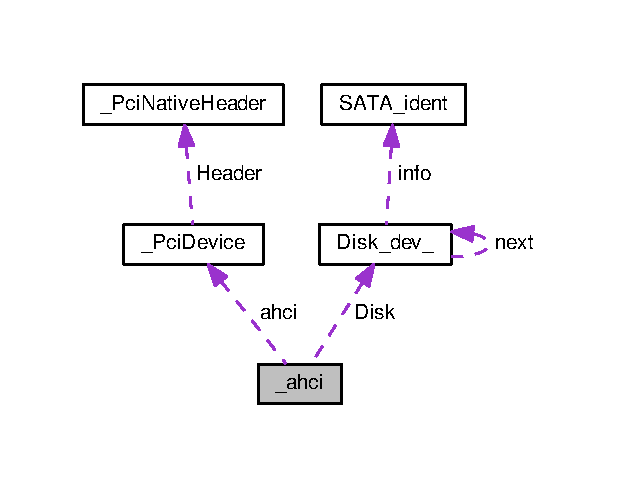
\includegraphics[width=297pt]{struct__ahci__coll__graph}
\end{center}
\end{figure}
\subsection*{Data Fields}
\begin{DoxyCompactItemize}
\item 
\hyperlink{PCI_8h_a9b8b354f1d0843a744762fc05dfc7366}{Pci\+Device\+\_\+t} $\ast$ \hyperlink{struct__ahci_ae21f72444b86864fa029b0386bce745c}{ahci}
\item 
unsigned short \hyperlink{struct__ahci_a767cb219a1220db83c0c934c5b9f260f}{Controller\+ID}
\item 
unsigned short \hyperlink{struct__ahci_a8964e69e694ed4ae3a4990889324eaa8}{Disks}
\item 
\hyperlink{ahci_8h_a56fc06d9da2a7877676381fa5d6e3f14}{Disk\+\_\+dev\+\_\+t} \hyperlink{struct__ahci_ae0b46ff5a72b27e8d91fa39d5bd70a74}{Disk} \mbox{[}32\mbox{]}
\end{DoxyCompactItemize}


\subsection{Detailed Description}


Definition at line 639 of file ahci.\+h.



\subsection{Field Documentation}
\index{\+\_\+ahci@{\+\_\+ahci}!ahci@{ahci}}
\index{ahci@{ahci}!\+\_\+ahci@{\+\_\+ahci}}
\subsubsection[{\texorpdfstring{ahci}{ahci}}]{\setlength{\rightskip}{0pt plus 5cm}{\bf Pci\+Device\+\_\+t}$\ast$ \+\_\+ahci\+::ahci}\hypertarget{struct__ahci_ae21f72444b86864fa029b0386bce745c}{}\label{struct__ahci_ae21f72444b86864fa029b0386bce745c}


Definition at line 641 of file ahci.\+h.

\index{\+\_\+ahci@{\+\_\+ahci}!Controller\+ID@{Controller\+ID}}
\index{Controller\+ID@{Controller\+ID}!\+\_\+ahci@{\+\_\+ahci}}
\subsubsection[{\texorpdfstring{Controller\+ID}{ControllerID}}]{\setlength{\rightskip}{0pt plus 5cm}unsigned short \+\_\+ahci\+::\+Controller\+ID}\hypertarget{struct__ahci_a767cb219a1220db83c0c934c5b9f260f}{}\label{struct__ahci_a767cb219a1220db83c0c934c5b9f260f}


Definition at line 642 of file ahci.\+h.

\index{\+\_\+ahci@{\+\_\+ahci}!Disk@{Disk}}
\index{Disk@{Disk}!\+\_\+ahci@{\+\_\+ahci}}
\subsubsection[{\texorpdfstring{Disk}{Disk}}]{\setlength{\rightskip}{0pt plus 5cm}{\bf Disk\+\_\+dev\+\_\+t} \+\_\+ahci\+::\+Disk\mbox{[}32\mbox{]}}\hypertarget{struct__ahci_ae0b46ff5a72b27e8d91fa39d5bd70a74}{}\label{struct__ahci_ae0b46ff5a72b27e8d91fa39d5bd70a74}


Definition at line 644 of file ahci.\+h.

\index{\+\_\+ahci@{\+\_\+ahci}!Disks@{Disks}}
\index{Disks@{Disks}!\+\_\+ahci@{\+\_\+ahci}}
\subsubsection[{\texorpdfstring{Disks}{Disks}}]{\setlength{\rightskip}{0pt plus 5cm}unsigned short \+\_\+ahci\+::\+Disks}\hypertarget{struct__ahci_a8964e69e694ed4ae3a4990889324eaa8}{}\label{struct__ahci_a8964e69e694ed4ae3a4990889324eaa8}


Definition at line 643 of file ahci.\+h.



The documentation for this struct was generated from the following file\+:\begin{DoxyCompactItemize}
\item 
Experimental Edition/\+Source/\+Drivers/\+A\+H\+C\+I/\hyperlink{ahci_8h}{ahci.\+h}\end{DoxyCompactItemize}

\hypertarget{struct__BIOS__PARAMATER__BLOCK}{}\section{\+\_\+\+B\+I\+O\+S\+\_\+\+P\+A\+R\+A\+M\+A\+T\+E\+R\+\_\+\+B\+L\+O\+CK Struct Reference}
\label{struct__BIOS__PARAMATER__BLOCK}\index{\+\_\+\+B\+I\+O\+S\+\_\+\+P\+A\+R\+A\+M\+A\+T\+E\+R\+\_\+\+B\+L\+O\+CK@{\+\_\+\+B\+I\+O\+S\+\_\+\+P\+A\+R\+A\+M\+A\+T\+E\+R\+\_\+\+B\+L\+O\+CK}}


{\ttfamily \#include $<$bpb.\+h$>$}

\subsection*{Data Fields}
\begin{DoxyCompactItemize}
\item 
uint8\+\_\+t \hyperlink{struct__BIOS__PARAMATER__BLOCK_a26e26852f15470344d8f29193a91b35c}{O\+E\+M\+Name} \mbox{[}8\mbox{]}
\item 
uint16\+\_\+t \hyperlink{struct__BIOS__PARAMATER__BLOCK_a66104ad70bc3243f824e6d3a5203017d}{Bytes\+Per\+Sector}
\item 
uint8\+\_\+t \hyperlink{struct__BIOS__PARAMATER__BLOCK_a32547c8a012ea20bff27d83f7dfeea97}{Sectors\+Per\+Cluster}
\item 
uint16\+\_\+t \hyperlink{struct__BIOS__PARAMATER__BLOCK_a9bc98792061fb38071840cc6c61d4bd9}{Reserved\+Sectors}
\item 
uint8\+\_\+t \hyperlink{struct__BIOS__PARAMATER__BLOCK_a19dde0c3c6c8dd2d20ef53bc9dc71da8}{Number\+Of\+Fats}
\item 
uint16\+\_\+t \hyperlink{struct__BIOS__PARAMATER__BLOCK_a9d9f79e3acd72e08ff27fb471569c841}{Num\+Dir\+Entries}
\item 
uint16\+\_\+t \hyperlink{struct__BIOS__PARAMATER__BLOCK_a98d94e48588132acbd65fedd4de95647}{Num\+Sectors}
\item 
uint8\+\_\+t \hyperlink{struct__BIOS__PARAMATER__BLOCK_a8b01f1d4dd34a1ef4c42a5ab83d3bf04}{Media}
\item 
uint16\+\_\+t \hyperlink{struct__BIOS__PARAMATER__BLOCK_adc667cf101250030eb318e36b38487ea}{Sectors\+Per\+Fat}
\item 
uint16\+\_\+t \hyperlink{struct__BIOS__PARAMATER__BLOCK_a78ea312224353e262bc1c1af91f4ccde}{Sectors\+Per\+Track}
\item 
uint16\+\_\+t \hyperlink{struct__BIOS__PARAMATER__BLOCK_a71a6800e1d31abe25b353b5b9b84c545}{Heads\+Per\+Cyl}
\item 
uint32\+\_\+t \hyperlink{struct__BIOS__PARAMATER__BLOCK_ad31ae2c22a4f844d1b9be9f1d7034a31}{Hidden\+Sectors}
\item 
uint32\+\_\+t \hyperlink{struct__BIOS__PARAMATER__BLOCK_a5b718eec0b4cb2f08ba2ec2578906e8a}{Long\+Sectors}
\end{DoxyCompactItemize}


\subsection{Detailed Description}
bios paramater block 

Definition at line 13 of file bpb.\+h.



\subsection{Field Documentation}
\index{\+\_\+\+B\+I\+O\+S\+\_\+\+P\+A\+R\+A\+M\+A\+T\+E\+R\+\_\+\+B\+L\+O\+CK@{\+\_\+\+B\+I\+O\+S\+\_\+\+P\+A\+R\+A\+M\+A\+T\+E\+R\+\_\+\+B\+L\+O\+CK}!Bytes\+Per\+Sector@{Bytes\+Per\+Sector}}
\index{Bytes\+Per\+Sector@{Bytes\+Per\+Sector}!\+\_\+\+B\+I\+O\+S\+\_\+\+P\+A\+R\+A\+M\+A\+T\+E\+R\+\_\+\+B\+L\+O\+CK@{\+\_\+\+B\+I\+O\+S\+\_\+\+P\+A\+R\+A\+M\+A\+T\+E\+R\+\_\+\+B\+L\+O\+CK}}
\subsubsection[{\texorpdfstring{Bytes\+Per\+Sector}{BytesPerSector}}]{\setlength{\rightskip}{0pt plus 5cm}uint16\+\_\+t \+\_\+\+B\+I\+O\+S\+\_\+\+P\+A\+R\+A\+M\+A\+T\+E\+R\+\_\+\+B\+L\+O\+C\+K\+::\+Bytes\+Per\+Sector}\hypertarget{struct__BIOS__PARAMATER__BLOCK_a66104ad70bc3243f824e6d3a5203017d}{}\label{struct__BIOS__PARAMATER__BLOCK_a66104ad70bc3243f824e6d3a5203017d}


Definition at line 16 of file bpb.\+h.

\index{\+\_\+\+B\+I\+O\+S\+\_\+\+P\+A\+R\+A\+M\+A\+T\+E\+R\+\_\+\+B\+L\+O\+CK@{\+\_\+\+B\+I\+O\+S\+\_\+\+P\+A\+R\+A\+M\+A\+T\+E\+R\+\_\+\+B\+L\+O\+CK}!Heads\+Per\+Cyl@{Heads\+Per\+Cyl}}
\index{Heads\+Per\+Cyl@{Heads\+Per\+Cyl}!\+\_\+\+B\+I\+O\+S\+\_\+\+P\+A\+R\+A\+M\+A\+T\+E\+R\+\_\+\+B\+L\+O\+CK@{\+\_\+\+B\+I\+O\+S\+\_\+\+P\+A\+R\+A\+M\+A\+T\+E\+R\+\_\+\+B\+L\+O\+CK}}
\subsubsection[{\texorpdfstring{Heads\+Per\+Cyl}{HeadsPerCyl}}]{\setlength{\rightskip}{0pt plus 5cm}uint16\+\_\+t \+\_\+\+B\+I\+O\+S\+\_\+\+P\+A\+R\+A\+M\+A\+T\+E\+R\+\_\+\+B\+L\+O\+C\+K\+::\+Heads\+Per\+Cyl}\hypertarget{struct__BIOS__PARAMATER__BLOCK_a71a6800e1d31abe25b353b5b9b84c545}{}\label{struct__BIOS__PARAMATER__BLOCK_a71a6800e1d31abe25b353b5b9b84c545}


Definition at line 25 of file bpb.\+h.

\index{\+\_\+\+B\+I\+O\+S\+\_\+\+P\+A\+R\+A\+M\+A\+T\+E\+R\+\_\+\+B\+L\+O\+CK@{\+\_\+\+B\+I\+O\+S\+\_\+\+P\+A\+R\+A\+M\+A\+T\+E\+R\+\_\+\+B\+L\+O\+CK}!Hidden\+Sectors@{Hidden\+Sectors}}
\index{Hidden\+Sectors@{Hidden\+Sectors}!\+\_\+\+B\+I\+O\+S\+\_\+\+P\+A\+R\+A\+M\+A\+T\+E\+R\+\_\+\+B\+L\+O\+CK@{\+\_\+\+B\+I\+O\+S\+\_\+\+P\+A\+R\+A\+M\+A\+T\+E\+R\+\_\+\+B\+L\+O\+CK}}
\subsubsection[{\texorpdfstring{Hidden\+Sectors}{HiddenSectors}}]{\setlength{\rightskip}{0pt plus 5cm}uint32\+\_\+t \+\_\+\+B\+I\+O\+S\+\_\+\+P\+A\+R\+A\+M\+A\+T\+E\+R\+\_\+\+B\+L\+O\+C\+K\+::\+Hidden\+Sectors}\hypertarget{struct__BIOS__PARAMATER__BLOCK_ad31ae2c22a4f844d1b9be9f1d7034a31}{}\label{struct__BIOS__PARAMATER__BLOCK_ad31ae2c22a4f844d1b9be9f1d7034a31}


Definition at line 26 of file bpb.\+h.

\index{\+\_\+\+B\+I\+O\+S\+\_\+\+P\+A\+R\+A\+M\+A\+T\+E\+R\+\_\+\+B\+L\+O\+CK@{\+\_\+\+B\+I\+O\+S\+\_\+\+P\+A\+R\+A\+M\+A\+T\+E\+R\+\_\+\+B\+L\+O\+CK}!Long\+Sectors@{Long\+Sectors}}
\index{Long\+Sectors@{Long\+Sectors}!\+\_\+\+B\+I\+O\+S\+\_\+\+P\+A\+R\+A\+M\+A\+T\+E\+R\+\_\+\+B\+L\+O\+CK@{\+\_\+\+B\+I\+O\+S\+\_\+\+P\+A\+R\+A\+M\+A\+T\+E\+R\+\_\+\+B\+L\+O\+CK}}
\subsubsection[{\texorpdfstring{Long\+Sectors}{LongSectors}}]{\setlength{\rightskip}{0pt plus 5cm}uint32\+\_\+t \+\_\+\+B\+I\+O\+S\+\_\+\+P\+A\+R\+A\+M\+A\+T\+E\+R\+\_\+\+B\+L\+O\+C\+K\+::\+Long\+Sectors}\hypertarget{struct__BIOS__PARAMATER__BLOCK_a5b718eec0b4cb2f08ba2ec2578906e8a}{}\label{struct__BIOS__PARAMATER__BLOCK_a5b718eec0b4cb2f08ba2ec2578906e8a}


Definition at line 27 of file bpb.\+h.

\index{\+\_\+\+B\+I\+O\+S\+\_\+\+P\+A\+R\+A\+M\+A\+T\+E\+R\+\_\+\+B\+L\+O\+CK@{\+\_\+\+B\+I\+O\+S\+\_\+\+P\+A\+R\+A\+M\+A\+T\+E\+R\+\_\+\+B\+L\+O\+CK}!Media@{Media}}
\index{Media@{Media}!\+\_\+\+B\+I\+O\+S\+\_\+\+P\+A\+R\+A\+M\+A\+T\+E\+R\+\_\+\+B\+L\+O\+CK@{\+\_\+\+B\+I\+O\+S\+\_\+\+P\+A\+R\+A\+M\+A\+T\+E\+R\+\_\+\+B\+L\+O\+CK}}
\subsubsection[{\texorpdfstring{Media}{Media}}]{\setlength{\rightskip}{0pt plus 5cm}uint8\+\_\+t \+\_\+\+B\+I\+O\+S\+\_\+\+P\+A\+R\+A\+M\+A\+T\+E\+R\+\_\+\+B\+L\+O\+C\+K\+::\+Media}\hypertarget{struct__BIOS__PARAMATER__BLOCK_a8b01f1d4dd34a1ef4c42a5ab83d3bf04}{}\label{struct__BIOS__PARAMATER__BLOCK_a8b01f1d4dd34a1ef4c42a5ab83d3bf04}


Definition at line 22 of file bpb.\+h.

\index{\+\_\+\+B\+I\+O\+S\+\_\+\+P\+A\+R\+A\+M\+A\+T\+E\+R\+\_\+\+B\+L\+O\+CK@{\+\_\+\+B\+I\+O\+S\+\_\+\+P\+A\+R\+A\+M\+A\+T\+E\+R\+\_\+\+B\+L\+O\+CK}!Number\+Of\+Fats@{Number\+Of\+Fats}}
\index{Number\+Of\+Fats@{Number\+Of\+Fats}!\+\_\+\+B\+I\+O\+S\+\_\+\+P\+A\+R\+A\+M\+A\+T\+E\+R\+\_\+\+B\+L\+O\+CK@{\+\_\+\+B\+I\+O\+S\+\_\+\+P\+A\+R\+A\+M\+A\+T\+E\+R\+\_\+\+B\+L\+O\+CK}}
\subsubsection[{\texorpdfstring{Number\+Of\+Fats}{NumberOfFats}}]{\setlength{\rightskip}{0pt plus 5cm}uint8\+\_\+t \+\_\+\+B\+I\+O\+S\+\_\+\+P\+A\+R\+A\+M\+A\+T\+E\+R\+\_\+\+B\+L\+O\+C\+K\+::\+Number\+Of\+Fats}\hypertarget{struct__BIOS__PARAMATER__BLOCK_a19dde0c3c6c8dd2d20ef53bc9dc71da8}{}\label{struct__BIOS__PARAMATER__BLOCK_a19dde0c3c6c8dd2d20ef53bc9dc71da8}


Definition at line 19 of file bpb.\+h.

\index{\+\_\+\+B\+I\+O\+S\+\_\+\+P\+A\+R\+A\+M\+A\+T\+E\+R\+\_\+\+B\+L\+O\+CK@{\+\_\+\+B\+I\+O\+S\+\_\+\+P\+A\+R\+A\+M\+A\+T\+E\+R\+\_\+\+B\+L\+O\+CK}!Num\+Dir\+Entries@{Num\+Dir\+Entries}}
\index{Num\+Dir\+Entries@{Num\+Dir\+Entries}!\+\_\+\+B\+I\+O\+S\+\_\+\+P\+A\+R\+A\+M\+A\+T\+E\+R\+\_\+\+B\+L\+O\+CK@{\+\_\+\+B\+I\+O\+S\+\_\+\+P\+A\+R\+A\+M\+A\+T\+E\+R\+\_\+\+B\+L\+O\+CK}}
\subsubsection[{\texorpdfstring{Num\+Dir\+Entries}{NumDirEntries}}]{\setlength{\rightskip}{0pt plus 5cm}uint16\+\_\+t \+\_\+\+B\+I\+O\+S\+\_\+\+P\+A\+R\+A\+M\+A\+T\+E\+R\+\_\+\+B\+L\+O\+C\+K\+::\+Num\+Dir\+Entries}\hypertarget{struct__BIOS__PARAMATER__BLOCK_a9d9f79e3acd72e08ff27fb471569c841}{}\label{struct__BIOS__PARAMATER__BLOCK_a9d9f79e3acd72e08ff27fb471569c841}


Definition at line 20 of file bpb.\+h.

\index{\+\_\+\+B\+I\+O\+S\+\_\+\+P\+A\+R\+A\+M\+A\+T\+E\+R\+\_\+\+B\+L\+O\+CK@{\+\_\+\+B\+I\+O\+S\+\_\+\+P\+A\+R\+A\+M\+A\+T\+E\+R\+\_\+\+B\+L\+O\+CK}!Num\+Sectors@{Num\+Sectors}}
\index{Num\+Sectors@{Num\+Sectors}!\+\_\+\+B\+I\+O\+S\+\_\+\+P\+A\+R\+A\+M\+A\+T\+E\+R\+\_\+\+B\+L\+O\+CK@{\+\_\+\+B\+I\+O\+S\+\_\+\+P\+A\+R\+A\+M\+A\+T\+E\+R\+\_\+\+B\+L\+O\+CK}}
\subsubsection[{\texorpdfstring{Num\+Sectors}{NumSectors}}]{\setlength{\rightskip}{0pt plus 5cm}uint16\+\_\+t \+\_\+\+B\+I\+O\+S\+\_\+\+P\+A\+R\+A\+M\+A\+T\+E\+R\+\_\+\+B\+L\+O\+C\+K\+::\+Num\+Sectors}\hypertarget{struct__BIOS__PARAMATER__BLOCK_a98d94e48588132acbd65fedd4de95647}{}\label{struct__BIOS__PARAMATER__BLOCK_a98d94e48588132acbd65fedd4de95647}


Definition at line 21 of file bpb.\+h.

\index{\+\_\+\+B\+I\+O\+S\+\_\+\+P\+A\+R\+A\+M\+A\+T\+E\+R\+\_\+\+B\+L\+O\+CK@{\+\_\+\+B\+I\+O\+S\+\_\+\+P\+A\+R\+A\+M\+A\+T\+E\+R\+\_\+\+B\+L\+O\+CK}!O\+E\+M\+Name@{O\+E\+M\+Name}}
\index{O\+E\+M\+Name@{O\+E\+M\+Name}!\+\_\+\+B\+I\+O\+S\+\_\+\+P\+A\+R\+A\+M\+A\+T\+E\+R\+\_\+\+B\+L\+O\+CK@{\+\_\+\+B\+I\+O\+S\+\_\+\+P\+A\+R\+A\+M\+A\+T\+E\+R\+\_\+\+B\+L\+O\+CK}}
\subsubsection[{\texorpdfstring{O\+E\+M\+Name}{OEMName}}]{\setlength{\rightskip}{0pt plus 5cm}uint8\+\_\+t \+\_\+\+B\+I\+O\+S\+\_\+\+P\+A\+R\+A\+M\+A\+T\+E\+R\+\_\+\+B\+L\+O\+C\+K\+::\+O\+E\+M\+Name\mbox{[}8\mbox{]}}\hypertarget{struct__BIOS__PARAMATER__BLOCK_a26e26852f15470344d8f29193a91b35c}{}\label{struct__BIOS__PARAMATER__BLOCK_a26e26852f15470344d8f29193a91b35c}


Definition at line 15 of file bpb.\+h.

\index{\+\_\+\+B\+I\+O\+S\+\_\+\+P\+A\+R\+A\+M\+A\+T\+E\+R\+\_\+\+B\+L\+O\+CK@{\+\_\+\+B\+I\+O\+S\+\_\+\+P\+A\+R\+A\+M\+A\+T\+E\+R\+\_\+\+B\+L\+O\+CK}!Reserved\+Sectors@{Reserved\+Sectors}}
\index{Reserved\+Sectors@{Reserved\+Sectors}!\+\_\+\+B\+I\+O\+S\+\_\+\+P\+A\+R\+A\+M\+A\+T\+E\+R\+\_\+\+B\+L\+O\+CK@{\+\_\+\+B\+I\+O\+S\+\_\+\+P\+A\+R\+A\+M\+A\+T\+E\+R\+\_\+\+B\+L\+O\+CK}}
\subsubsection[{\texorpdfstring{Reserved\+Sectors}{ReservedSectors}}]{\setlength{\rightskip}{0pt plus 5cm}uint16\+\_\+t \+\_\+\+B\+I\+O\+S\+\_\+\+P\+A\+R\+A\+M\+A\+T\+E\+R\+\_\+\+B\+L\+O\+C\+K\+::\+Reserved\+Sectors}\hypertarget{struct__BIOS__PARAMATER__BLOCK_a9bc98792061fb38071840cc6c61d4bd9}{}\label{struct__BIOS__PARAMATER__BLOCK_a9bc98792061fb38071840cc6c61d4bd9}


Definition at line 18 of file bpb.\+h.

\index{\+\_\+\+B\+I\+O\+S\+\_\+\+P\+A\+R\+A\+M\+A\+T\+E\+R\+\_\+\+B\+L\+O\+CK@{\+\_\+\+B\+I\+O\+S\+\_\+\+P\+A\+R\+A\+M\+A\+T\+E\+R\+\_\+\+B\+L\+O\+CK}!Sectors\+Per\+Cluster@{Sectors\+Per\+Cluster}}
\index{Sectors\+Per\+Cluster@{Sectors\+Per\+Cluster}!\+\_\+\+B\+I\+O\+S\+\_\+\+P\+A\+R\+A\+M\+A\+T\+E\+R\+\_\+\+B\+L\+O\+CK@{\+\_\+\+B\+I\+O\+S\+\_\+\+P\+A\+R\+A\+M\+A\+T\+E\+R\+\_\+\+B\+L\+O\+CK}}
\subsubsection[{\texorpdfstring{Sectors\+Per\+Cluster}{SectorsPerCluster}}]{\setlength{\rightskip}{0pt plus 5cm}uint8\+\_\+t \+\_\+\+B\+I\+O\+S\+\_\+\+P\+A\+R\+A\+M\+A\+T\+E\+R\+\_\+\+B\+L\+O\+C\+K\+::\+Sectors\+Per\+Cluster}\hypertarget{struct__BIOS__PARAMATER__BLOCK_a32547c8a012ea20bff27d83f7dfeea97}{}\label{struct__BIOS__PARAMATER__BLOCK_a32547c8a012ea20bff27d83f7dfeea97}


Definition at line 17 of file bpb.\+h.

\index{\+\_\+\+B\+I\+O\+S\+\_\+\+P\+A\+R\+A\+M\+A\+T\+E\+R\+\_\+\+B\+L\+O\+CK@{\+\_\+\+B\+I\+O\+S\+\_\+\+P\+A\+R\+A\+M\+A\+T\+E\+R\+\_\+\+B\+L\+O\+CK}!Sectors\+Per\+Fat@{Sectors\+Per\+Fat}}
\index{Sectors\+Per\+Fat@{Sectors\+Per\+Fat}!\+\_\+\+B\+I\+O\+S\+\_\+\+P\+A\+R\+A\+M\+A\+T\+E\+R\+\_\+\+B\+L\+O\+CK@{\+\_\+\+B\+I\+O\+S\+\_\+\+P\+A\+R\+A\+M\+A\+T\+E\+R\+\_\+\+B\+L\+O\+CK}}
\subsubsection[{\texorpdfstring{Sectors\+Per\+Fat}{SectorsPerFat}}]{\setlength{\rightskip}{0pt plus 5cm}uint16\+\_\+t \+\_\+\+B\+I\+O\+S\+\_\+\+P\+A\+R\+A\+M\+A\+T\+E\+R\+\_\+\+B\+L\+O\+C\+K\+::\+Sectors\+Per\+Fat}\hypertarget{struct__BIOS__PARAMATER__BLOCK_adc667cf101250030eb318e36b38487ea}{}\label{struct__BIOS__PARAMATER__BLOCK_adc667cf101250030eb318e36b38487ea}


Definition at line 23 of file bpb.\+h.

\index{\+\_\+\+B\+I\+O\+S\+\_\+\+P\+A\+R\+A\+M\+A\+T\+E\+R\+\_\+\+B\+L\+O\+CK@{\+\_\+\+B\+I\+O\+S\+\_\+\+P\+A\+R\+A\+M\+A\+T\+E\+R\+\_\+\+B\+L\+O\+CK}!Sectors\+Per\+Track@{Sectors\+Per\+Track}}
\index{Sectors\+Per\+Track@{Sectors\+Per\+Track}!\+\_\+\+B\+I\+O\+S\+\_\+\+P\+A\+R\+A\+M\+A\+T\+E\+R\+\_\+\+B\+L\+O\+CK@{\+\_\+\+B\+I\+O\+S\+\_\+\+P\+A\+R\+A\+M\+A\+T\+E\+R\+\_\+\+B\+L\+O\+CK}}
\subsubsection[{\texorpdfstring{Sectors\+Per\+Track}{SectorsPerTrack}}]{\setlength{\rightskip}{0pt plus 5cm}uint16\+\_\+t \+\_\+\+B\+I\+O\+S\+\_\+\+P\+A\+R\+A\+M\+A\+T\+E\+R\+\_\+\+B\+L\+O\+C\+K\+::\+Sectors\+Per\+Track}\hypertarget{struct__BIOS__PARAMATER__BLOCK_a78ea312224353e262bc1c1af91f4ccde}{}\label{struct__BIOS__PARAMATER__BLOCK_a78ea312224353e262bc1c1af91f4ccde}


Definition at line 24 of file bpb.\+h.



The documentation for this struct was generated from the following file\+:\begin{DoxyCompactItemize}
\item 
Experimental Edition/\+Source/vfs/\hyperlink{bpb_8h}{bpb.\+h}\end{DoxyCompactItemize}

\hypertarget{struct__BIOS__PARAMATER__BLOCK__EXT}{}\section{\+\_\+\+B\+I\+O\+S\+\_\+\+P\+A\+R\+A\+M\+A\+T\+E\+R\+\_\+\+B\+L\+O\+C\+K\+\_\+\+E\+XT Struct Reference}
\label{struct__BIOS__PARAMATER__BLOCK__EXT}\index{\+\_\+\+B\+I\+O\+S\+\_\+\+P\+A\+R\+A\+M\+A\+T\+E\+R\+\_\+\+B\+L\+O\+C\+K\+\_\+\+E\+XT@{\+\_\+\+B\+I\+O\+S\+\_\+\+P\+A\+R\+A\+M\+A\+T\+E\+R\+\_\+\+B\+L\+O\+C\+K\+\_\+\+E\+XT}}


{\ttfamily \#include $<$bpb.\+h$>$}

\subsection*{Data Fields}
\begin{DoxyCompactItemize}
\item 
uint32\+\_\+t \hyperlink{struct__BIOS__PARAMATER__BLOCK__EXT_acfed1dbed7039b6789e6351ebacee24a}{Sectors\+Per\+Fat32}
\item 
uint16\+\_\+t \hyperlink{struct__BIOS__PARAMATER__BLOCK__EXT_a792e2adce56f9d75b1ae4b7a072da57f}{Flags}
\item 
uint16\+\_\+t \hyperlink{struct__BIOS__PARAMATER__BLOCK__EXT_a75c0e772bb6d509159a7ddb90f1567a7}{Version}
\item 
uint32\+\_\+t \hyperlink{struct__BIOS__PARAMATER__BLOCK__EXT_aac74e28a6f93ca8e26d8675ef150487e}{Root\+Cluster}
\item 
uint16\+\_\+t \hyperlink{struct__BIOS__PARAMATER__BLOCK__EXT_a0ece333302e2be2993066c7b69b4a3c6}{Info\+Cluster}
\item 
uint16\+\_\+t \hyperlink{struct__BIOS__PARAMATER__BLOCK__EXT_a6d35f095d874ab3b5f12ad6d79efc2a7}{Backup\+Boot}
\item 
uint16\+\_\+t \hyperlink{struct__BIOS__PARAMATER__BLOCK__EXT_a49ffb182c5b3f929ab64f7b502237bfe}{Reserved} \mbox{[}6\mbox{]}
\end{DoxyCompactItemize}


\subsection{Detailed Description}
bios paramater block extended attributes 

Definition at line 34 of file bpb.\+h.



\subsection{Field Documentation}
\index{\+\_\+\+B\+I\+O\+S\+\_\+\+P\+A\+R\+A\+M\+A\+T\+E\+R\+\_\+\+B\+L\+O\+C\+K\+\_\+\+E\+XT@{\+\_\+\+B\+I\+O\+S\+\_\+\+P\+A\+R\+A\+M\+A\+T\+E\+R\+\_\+\+B\+L\+O\+C\+K\+\_\+\+E\+XT}!Backup\+Boot@{Backup\+Boot}}
\index{Backup\+Boot@{Backup\+Boot}!\+\_\+\+B\+I\+O\+S\+\_\+\+P\+A\+R\+A\+M\+A\+T\+E\+R\+\_\+\+B\+L\+O\+C\+K\+\_\+\+E\+XT@{\+\_\+\+B\+I\+O\+S\+\_\+\+P\+A\+R\+A\+M\+A\+T\+E\+R\+\_\+\+B\+L\+O\+C\+K\+\_\+\+E\+XT}}
\subsubsection[{\texorpdfstring{Backup\+Boot}{BackupBoot}}]{\setlength{\rightskip}{0pt plus 5cm}uint16\+\_\+t \+\_\+\+B\+I\+O\+S\+\_\+\+P\+A\+R\+A\+M\+A\+T\+E\+R\+\_\+\+B\+L\+O\+C\+K\+\_\+\+E\+X\+T\+::\+Backup\+Boot}\hypertarget{struct__BIOS__PARAMATER__BLOCK__EXT_a6d35f095d874ab3b5f12ad6d79efc2a7}{}\label{struct__BIOS__PARAMATER__BLOCK__EXT_a6d35f095d874ab3b5f12ad6d79efc2a7}


Definition at line 41 of file bpb.\+h.

\index{\+\_\+\+B\+I\+O\+S\+\_\+\+P\+A\+R\+A\+M\+A\+T\+E\+R\+\_\+\+B\+L\+O\+C\+K\+\_\+\+E\+XT@{\+\_\+\+B\+I\+O\+S\+\_\+\+P\+A\+R\+A\+M\+A\+T\+E\+R\+\_\+\+B\+L\+O\+C\+K\+\_\+\+E\+XT}!Flags@{Flags}}
\index{Flags@{Flags}!\+\_\+\+B\+I\+O\+S\+\_\+\+P\+A\+R\+A\+M\+A\+T\+E\+R\+\_\+\+B\+L\+O\+C\+K\+\_\+\+E\+XT@{\+\_\+\+B\+I\+O\+S\+\_\+\+P\+A\+R\+A\+M\+A\+T\+E\+R\+\_\+\+B\+L\+O\+C\+K\+\_\+\+E\+XT}}
\subsubsection[{\texorpdfstring{Flags}{Flags}}]{\setlength{\rightskip}{0pt plus 5cm}uint16\+\_\+t \+\_\+\+B\+I\+O\+S\+\_\+\+P\+A\+R\+A\+M\+A\+T\+E\+R\+\_\+\+B\+L\+O\+C\+K\+\_\+\+E\+X\+T\+::\+Flags}\hypertarget{struct__BIOS__PARAMATER__BLOCK__EXT_a792e2adce56f9d75b1ae4b7a072da57f}{}\label{struct__BIOS__PARAMATER__BLOCK__EXT_a792e2adce56f9d75b1ae4b7a072da57f}


Definition at line 37 of file bpb.\+h.

\index{\+\_\+\+B\+I\+O\+S\+\_\+\+P\+A\+R\+A\+M\+A\+T\+E\+R\+\_\+\+B\+L\+O\+C\+K\+\_\+\+E\+XT@{\+\_\+\+B\+I\+O\+S\+\_\+\+P\+A\+R\+A\+M\+A\+T\+E\+R\+\_\+\+B\+L\+O\+C\+K\+\_\+\+E\+XT}!Info\+Cluster@{Info\+Cluster}}
\index{Info\+Cluster@{Info\+Cluster}!\+\_\+\+B\+I\+O\+S\+\_\+\+P\+A\+R\+A\+M\+A\+T\+E\+R\+\_\+\+B\+L\+O\+C\+K\+\_\+\+E\+XT@{\+\_\+\+B\+I\+O\+S\+\_\+\+P\+A\+R\+A\+M\+A\+T\+E\+R\+\_\+\+B\+L\+O\+C\+K\+\_\+\+E\+XT}}
\subsubsection[{\texorpdfstring{Info\+Cluster}{InfoCluster}}]{\setlength{\rightskip}{0pt plus 5cm}uint16\+\_\+t \+\_\+\+B\+I\+O\+S\+\_\+\+P\+A\+R\+A\+M\+A\+T\+E\+R\+\_\+\+B\+L\+O\+C\+K\+\_\+\+E\+X\+T\+::\+Info\+Cluster}\hypertarget{struct__BIOS__PARAMATER__BLOCK__EXT_a0ece333302e2be2993066c7b69b4a3c6}{}\label{struct__BIOS__PARAMATER__BLOCK__EXT_a0ece333302e2be2993066c7b69b4a3c6}


Definition at line 40 of file bpb.\+h.

\index{\+\_\+\+B\+I\+O\+S\+\_\+\+P\+A\+R\+A\+M\+A\+T\+E\+R\+\_\+\+B\+L\+O\+C\+K\+\_\+\+E\+XT@{\+\_\+\+B\+I\+O\+S\+\_\+\+P\+A\+R\+A\+M\+A\+T\+E\+R\+\_\+\+B\+L\+O\+C\+K\+\_\+\+E\+XT}!Reserved@{Reserved}}
\index{Reserved@{Reserved}!\+\_\+\+B\+I\+O\+S\+\_\+\+P\+A\+R\+A\+M\+A\+T\+E\+R\+\_\+\+B\+L\+O\+C\+K\+\_\+\+E\+XT@{\+\_\+\+B\+I\+O\+S\+\_\+\+P\+A\+R\+A\+M\+A\+T\+E\+R\+\_\+\+B\+L\+O\+C\+K\+\_\+\+E\+XT}}
\subsubsection[{\texorpdfstring{Reserved}{Reserved}}]{\setlength{\rightskip}{0pt plus 5cm}uint16\+\_\+t \+\_\+\+B\+I\+O\+S\+\_\+\+P\+A\+R\+A\+M\+A\+T\+E\+R\+\_\+\+B\+L\+O\+C\+K\+\_\+\+E\+X\+T\+::\+Reserved\mbox{[}6\mbox{]}}\hypertarget{struct__BIOS__PARAMATER__BLOCK__EXT_a49ffb182c5b3f929ab64f7b502237bfe}{}\label{struct__BIOS__PARAMATER__BLOCK__EXT_a49ffb182c5b3f929ab64f7b502237bfe}


Definition at line 42 of file bpb.\+h.

\index{\+\_\+\+B\+I\+O\+S\+\_\+\+P\+A\+R\+A\+M\+A\+T\+E\+R\+\_\+\+B\+L\+O\+C\+K\+\_\+\+E\+XT@{\+\_\+\+B\+I\+O\+S\+\_\+\+P\+A\+R\+A\+M\+A\+T\+E\+R\+\_\+\+B\+L\+O\+C\+K\+\_\+\+E\+XT}!Root\+Cluster@{Root\+Cluster}}
\index{Root\+Cluster@{Root\+Cluster}!\+\_\+\+B\+I\+O\+S\+\_\+\+P\+A\+R\+A\+M\+A\+T\+E\+R\+\_\+\+B\+L\+O\+C\+K\+\_\+\+E\+XT@{\+\_\+\+B\+I\+O\+S\+\_\+\+P\+A\+R\+A\+M\+A\+T\+E\+R\+\_\+\+B\+L\+O\+C\+K\+\_\+\+E\+XT}}
\subsubsection[{\texorpdfstring{Root\+Cluster}{RootCluster}}]{\setlength{\rightskip}{0pt plus 5cm}uint32\+\_\+t \+\_\+\+B\+I\+O\+S\+\_\+\+P\+A\+R\+A\+M\+A\+T\+E\+R\+\_\+\+B\+L\+O\+C\+K\+\_\+\+E\+X\+T\+::\+Root\+Cluster}\hypertarget{struct__BIOS__PARAMATER__BLOCK__EXT_aac74e28a6f93ca8e26d8675ef150487e}{}\label{struct__BIOS__PARAMATER__BLOCK__EXT_aac74e28a6f93ca8e26d8675ef150487e}


Definition at line 39 of file bpb.\+h.

\index{\+\_\+\+B\+I\+O\+S\+\_\+\+P\+A\+R\+A\+M\+A\+T\+E\+R\+\_\+\+B\+L\+O\+C\+K\+\_\+\+E\+XT@{\+\_\+\+B\+I\+O\+S\+\_\+\+P\+A\+R\+A\+M\+A\+T\+E\+R\+\_\+\+B\+L\+O\+C\+K\+\_\+\+E\+XT}!Sectors\+Per\+Fat32@{Sectors\+Per\+Fat32}}
\index{Sectors\+Per\+Fat32@{Sectors\+Per\+Fat32}!\+\_\+\+B\+I\+O\+S\+\_\+\+P\+A\+R\+A\+M\+A\+T\+E\+R\+\_\+\+B\+L\+O\+C\+K\+\_\+\+E\+XT@{\+\_\+\+B\+I\+O\+S\+\_\+\+P\+A\+R\+A\+M\+A\+T\+E\+R\+\_\+\+B\+L\+O\+C\+K\+\_\+\+E\+XT}}
\subsubsection[{\texorpdfstring{Sectors\+Per\+Fat32}{SectorsPerFat32}}]{\setlength{\rightskip}{0pt plus 5cm}uint32\+\_\+t \+\_\+\+B\+I\+O\+S\+\_\+\+P\+A\+R\+A\+M\+A\+T\+E\+R\+\_\+\+B\+L\+O\+C\+K\+\_\+\+E\+X\+T\+::\+Sectors\+Per\+Fat32}\hypertarget{struct__BIOS__PARAMATER__BLOCK__EXT_acfed1dbed7039b6789e6351ebacee24a}{}\label{struct__BIOS__PARAMATER__BLOCK__EXT_acfed1dbed7039b6789e6351ebacee24a}


Definition at line 36 of file bpb.\+h.

\index{\+\_\+\+B\+I\+O\+S\+\_\+\+P\+A\+R\+A\+M\+A\+T\+E\+R\+\_\+\+B\+L\+O\+C\+K\+\_\+\+E\+XT@{\+\_\+\+B\+I\+O\+S\+\_\+\+P\+A\+R\+A\+M\+A\+T\+E\+R\+\_\+\+B\+L\+O\+C\+K\+\_\+\+E\+XT}!Version@{Version}}
\index{Version@{Version}!\+\_\+\+B\+I\+O\+S\+\_\+\+P\+A\+R\+A\+M\+A\+T\+E\+R\+\_\+\+B\+L\+O\+C\+K\+\_\+\+E\+XT@{\+\_\+\+B\+I\+O\+S\+\_\+\+P\+A\+R\+A\+M\+A\+T\+E\+R\+\_\+\+B\+L\+O\+C\+K\+\_\+\+E\+XT}}
\subsubsection[{\texorpdfstring{Version}{Version}}]{\setlength{\rightskip}{0pt plus 5cm}uint16\+\_\+t \+\_\+\+B\+I\+O\+S\+\_\+\+P\+A\+R\+A\+M\+A\+T\+E\+R\+\_\+\+B\+L\+O\+C\+K\+\_\+\+E\+X\+T\+::\+Version}\hypertarget{struct__BIOS__PARAMATER__BLOCK__EXT_a75c0e772bb6d509159a7ddb90f1567a7}{}\label{struct__BIOS__PARAMATER__BLOCK__EXT_a75c0e772bb6d509159a7ddb90f1567a7}


Definition at line 38 of file bpb.\+h.



The documentation for this struct was generated from the following file\+:\begin{DoxyCompactItemize}
\item 
Experimental Edition/\+Source/vfs/\hyperlink{bpb_8h}{bpb.\+h}\end{DoxyCompactItemize}

\hypertarget{struct__BOOT__SECTOR}{}\section{\+\_\+\+B\+O\+O\+T\+\_\+\+S\+E\+C\+T\+OR Struct Reference}
\label{struct__BOOT__SECTOR}\index{\+\_\+\+B\+O\+O\+T\+\_\+\+S\+E\+C\+T\+OR@{\+\_\+\+B\+O\+O\+T\+\_\+\+S\+E\+C\+T\+OR}}


{\ttfamily \#include $<$bpb.\+h$>$}



Collaboration diagram for \+\_\+\+B\+O\+O\+T\+\_\+\+S\+E\+C\+T\+OR\+:
\nopagebreak
\begin{figure}[H]
\begin{center}
\leavevmode
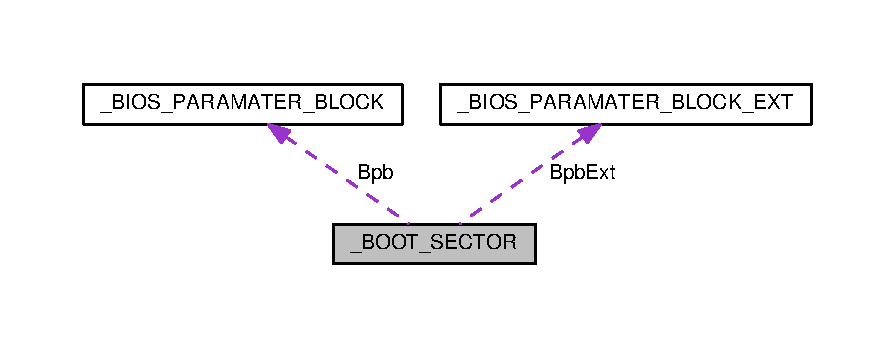
\includegraphics[width=350pt]{struct__BOOT__SECTOR__coll__graph}
\end{center}
\end{figure}
\subsection*{Data Fields}
\begin{DoxyCompactItemize}
\item 
uint8\+\_\+t \hyperlink{struct__BOOT__SECTOR_abcae473872a0324e463ab36564130d3d}{Ignore} \mbox{[}3\mbox{]}
\item 
\hyperlink{bpb_8h_af3ab7bfb42ad1b54891579f73be41bc1}{B\+I\+O\+S\+P\+A\+R\+A\+M\+A\+T\+E\+R\+B\+L\+O\+CK} \hyperlink{struct__BOOT__SECTOR_afedc563717fbacc0ce2e3b2fa31384bc}{Bpb}
\item 
\hyperlink{bpb_8h_a6da0cad454277100b4664773103a198d}{B\+I\+O\+S\+P\+A\+R\+A\+M\+A\+T\+E\+R\+B\+L\+O\+C\+K\+E\+XT} \hyperlink{struct__BOOT__SECTOR_ab175294dfdb20919b006865ac486df09}{Bpb\+Ext}
\item 
uint8\+\_\+t \hyperlink{struct__BOOT__SECTOR_abca94a8f55946d277eed33716aa8a612}{Filler} \mbox{[}448\mbox{]}
\end{DoxyCompactItemize}


\subsection{Detailed Description}
boot sector 

Definition at line 49 of file bpb.\+h.



\subsection{Field Documentation}
\index{\+\_\+\+B\+O\+O\+T\+\_\+\+S\+E\+C\+T\+OR@{\+\_\+\+B\+O\+O\+T\+\_\+\+S\+E\+C\+T\+OR}!Bpb@{Bpb}}
\index{Bpb@{Bpb}!\+\_\+\+B\+O\+O\+T\+\_\+\+S\+E\+C\+T\+OR@{\+\_\+\+B\+O\+O\+T\+\_\+\+S\+E\+C\+T\+OR}}
\subsubsection[{\texorpdfstring{Bpb}{Bpb}}]{\setlength{\rightskip}{0pt plus 5cm}{\bf B\+I\+O\+S\+P\+A\+R\+A\+M\+A\+T\+E\+R\+B\+L\+O\+CK} \+\_\+\+B\+O\+O\+T\+\_\+\+S\+E\+C\+T\+O\+R\+::\+Bpb}\hypertarget{struct__BOOT__SECTOR_afedc563717fbacc0ce2e3b2fa31384bc}{}\label{struct__BOOT__SECTOR_afedc563717fbacc0ce2e3b2fa31384bc}


Definition at line 52 of file bpb.\+h.

\index{\+\_\+\+B\+O\+O\+T\+\_\+\+S\+E\+C\+T\+OR@{\+\_\+\+B\+O\+O\+T\+\_\+\+S\+E\+C\+T\+OR}!Bpb\+Ext@{Bpb\+Ext}}
\index{Bpb\+Ext@{Bpb\+Ext}!\+\_\+\+B\+O\+O\+T\+\_\+\+S\+E\+C\+T\+OR@{\+\_\+\+B\+O\+O\+T\+\_\+\+S\+E\+C\+T\+OR}}
\subsubsection[{\texorpdfstring{Bpb\+Ext}{BpbExt}}]{\setlength{\rightskip}{0pt plus 5cm}{\bf B\+I\+O\+S\+P\+A\+R\+A\+M\+A\+T\+E\+R\+B\+L\+O\+C\+K\+E\+XT} \+\_\+\+B\+O\+O\+T\+\_\+\+S\+E\+C\+T\+O\+R\+::\+Bpb\+Ext}\hypertarget{struct__BOOT__SECTOR_ab175294dfdb20919b006865ac486df09}{}\label{struct__BOOT__SECTOR_ab175294dfdb20919b006865ac486df09}


Definition at line 53 of file bpb.\+h.

\index{\+\_\+\+B\+O\+O\+T\+\_\+\+S\+E\+C\+T\+OR@{\+\_\+\+B\+O\+O\+T\+\_\+\+S\+E\+C\+T\+OR}!Filler@{Filler}}
\index{Filler@{Filler}!\+\_\+\+B\+O\+O\+T\+\_\+\+S\+E\+C\+T\+OR@{\+\_\+\+B\+O\+O\+T\+\_\+\+S\+E\+C\+T\+OR}}
\subsubsection[{\texorpdfstring{Filler}{Filler}}]{\setlength{\rightskip}{0pt plus 5cm}uint8\+\_\+t \+\_\+\+B\+O\+O\+T\+\_\+\+S\+E\+C\+T\+O\+R\+::\+Filler\mbox{[}448\mbox{]}}\hypertarget{struct__BOOT__SECTOR_abca94a8f55946d277eed33716aa8a612}{}\label{struct__BOOT__SECTOR_abca94a8f55946d277eed33716aa8a612}


Definition at line 54 of file bpb.\+h.

\index{\+\_\+\+B\+O\+O\+T\+\_\+\+S\+E\+C\+T\+OR@{\+\_\+\+B\+O\+O\+T\+\_\+\+S\+E\+C\+T\+OR}!Ignore@{Ignore}}
\index{Ignore@{Ignore}!\+\_\+\+B\+O\+O\+T\+\_\+\+S\+E\+C\+T\+OR@{\+\_\+\+B\+O\+O\+T\+\_\+\+S\+E\+C\+T\+OR}}
\subsubsection[{\texorpdfstring{Ignore}{Ignore}}]{\setlength{\rightskip}{0pt plus 5cm}uint8\+\_\+t \+\_\+\+B\+O\+O\+T\+\_\+\+S\+E\+C\+T\+O\+R\+::\+Ignore\mbox{[}3\mbox{]}}\hypertarget{struct__BOOT__SECTOR_abcae473872a0324e463ab36564130d3d}{}\label{struct__BOOT__SECTOR_abcae473872a0324e463ab36564130d3d}


Definition at line 51 of file bpb.\+h.



The documentation for this struct was generated from the following file\+:\begin{DoxyCompactItemize}
\item 
Experimental Edition/\+Source/vfs/\hyperlink{bpb_8h}{bpb.\+h}\end{DoxyCompactItemize}

\hypertarget{struct__DIRECTORY}{}\section{\+\_\+\+D\+I\+R\+E\+C\+T\+O\+RY Struct Reference}
\label{struct__DIRECTORY}\index{\+\_\+\+D\+I\+R\+E\+C\+T\+O\+RY@{\+\_\+\+D\+I\+R\+E\+C\+T\+O\+RY}}


{\ttfamily \#include $<$fat.\+h$>$}

\subsection*{Data Fields}
\begin{DoxyCompactItemize}
\item 
uint8\+\_\+t \hyperlink{struct__DIRECTORY_ab9950ebc3a840e0ad44f1aa3e2a05be6}{Filename} \mbox{[}8\mbox{]}
\item 
uint8\+\_\+t \hyperlink{struct__DIRECTORY_ac29a0cf993ecea88a7b7a4050be9b025}{Ext} \mbox{[}3\mbox{]}
\item 
uint8\+\_\+t \hyperlink{struct__DIRECTORY_a01c9dc5d98375e3205b87b3188165413}{Attrib}
\item 
uint8\+\_\+t \hyperlink{struct__DIRECTORY_a0c6a3f809355165500632158bb89273c}{Reserved}
\item 
uint8\+\_\+t \hyperlink{struct__DIRECTORY_a5fea072b6e2e5b9c1921d6d04f9ab5e9}{Time\+Created\+Ms}
\item 
uint16\+\_\+t \hyperlink{struct__DIRECTORY_a6eda82476c383777293ee3ec945537d7}{Time\+Created}
\item 
uint16\+\_\+t \hyperlink{struct__DIRECTORY_a7a4fe27d7f0751594dd0d7f458c5dff0}{Date\+Created}
\item 
uint16\+\_\+t \hyperlink{struct__DIRECTORY_a779c681de0304d76409a3783cafda05c}{Date\+Last\+Accessed}
\item 
uint16\+\_\+t \hyperlink{struct__DIRECTORY_ae62a72d82aa0203065f37196210a0de5}{First\+Cluster\+Hi\+Bytes}
\item 
uint16\+\_\+t \hyperlink{struct__DIRECTORY_ac628fc1cc05972577424858d0046345d}{Last\+Mod\+Time}
\item 
uint16\+\_\+t \hyperlink{struct__DIRECTORY_a84aa4428dc379a985fba877a88f41d89}{Last\+Mod\+Date}
\item 
uint16\+\_\+t \hyperlink{struct__DIRECTORY_a587e8955f97e6b4bac5f0f0778e08a4f}{First\+Cluster}
\item 
uint32\+\_\+t \hyperlink{struct__DIRECTORY_a7e15691413cbea31518a0d989de5ff0e}{File\+Size}
\end{DoxyCompactItemize}


\subsection{Detailed Description}


Definition at line 7 of file fat.\+h.



\subsection{Field Documentation}
\index{\+\_\+\+D\+I\+R\+E\+C\+T\+O\+RY@{\+\_\+\+D\+I\+R\+E\+C\+T\+O\+RY}!Attrib@{Attrib}}
\index{Attrib@{Attrib}!\+\_\+\+D\+I\+R\+E\+C\+T\+O\+RY@{\+\_\+\+D\+I\+R\+E\+C\+T\+O\+RY}}
\subsubsection[{\texorpdfstring{Attrib}{Attrib}}]{\setlength{\rightskip}{0pt plus 5cm}uint8\+\_\+t \+\_\+\+D\+I\+R\+E\+C\+T\+O\+R\+Y\+::\+Attrib}\hypertarget{struct__DIRECTORY_a01c9dc5d98375e3205b87b3188165413}{}\label{struct__DIRECTORY_a01c9dc5d98375e3205b87b3188165413}


Definition at line 11 of file fat.\+h.

\index{\+\_\+\+D\+I\+R\+E\+C\+T\+O\+RY@{\+\_\+\+D\+I\+R\+E\+C\+T\+O\+RY}!Date\+Created@{Date\+Created}}
\index{Date\+Created@{Date\+Created}!\+\_\+\+D\+I\+R\+E\+C\+T\+O\+RY@{\+\_\+\+D\+I\+R\+E\+C\+T\+O\+RY}}
\subsubsection[{\texorpdfstring{Date\+Created}{DateCreated}}]{\setlength{\rightskip}{0pt plus 5cm}uint16\+\_\+t \+\_\+\+D\+I\+R\+E\+C\+T\+O\+R\+Y\+::\+Date\+Created}\hypertarget{struct__DIRECTORY_a7a4fe27d7f0751594dd0d7f458c5dff0}{}\label{struct__DIRECTORY_a7a4fe27d7f0751594dd0d7f458c5dff0}


Definition at line 15 of file fat.\+h.

\index{\+\_\+\+D\+I\+R\+E\+C\+T\+O\+RY@{\+\_\+\+D\+I\+R\+E\+C\+T\+O\+RY}!Date\+Last\+Accessed@{Date\+Last\+Accessed}}
\index{Date\+Last\+Accessed@{Date\+Last\+Accessed}!\+\_\+\+D\+I\+R\+E\+C\+T\+O\+RY@{\+\_\+\+D\+I\+R\+E\+C\+T\+O\+RY}}
\subsubsection[{\texorpdfstring{Date\+Last\+Accessed}{DateLastAccessed}}]{\setlength{\rightskip}{0pt plus 5cm}uint16\+\_\+t \+\_\+\+D\+I\+R\+E\+C\+T\+O\+R\+Y\+::\+Date\+Last\+Accessed}\hypertarget{struct__DIRECTORY_a779c681de0304d76409a3783cafda05c}{}\label{struct__DIRECTORY_a779c681de0304d76409a3783cafda05c}


Definition at line 16 of file fat.\+h.

\index{\+\_\+\+D\+I\+R\+E\+C\+T\+O\+RY@{\+\_\+\+D\+I\+R\+E\+C\+T\+O\+RY}!Ext@{Ext}}
\index{Ext@{Ext}!\+\_\+\+D\+I\+R\+E\+C\+T\+O\+RY@{\+\_\+\+D\+I\+R\+E\+C\+T\+O\+RY}}
\subsubsection[{\texorpdfstring{Ext}{Ext}}]{\setlength{\rightskip}{0pt plus 5cm}uint8\+\_\+t \+\_\+\+D\+I\+R\+E\+C\+T\+O\+R\+Y\+::\+Ext\mbox{[}3\mbox{]}}\hypertarget{struct__DIRECTORY_ac29a0cf993ecea88a7b7a4050be9b025}{}\label{struct__DIRECTORY_ac29a0cf993ecea88a7b7a4050be9b025}


Definition at line 10 of file fat.\+h.

\index{\+\_\+\+D\+I\+R\+E\+C\+T\+O\+RY@{\+\_\+\+D\+I\+R\+E\+C\+T\+O\+RY}!Filename@{Filename}}
\index{Filename@{Filename}!\+\_\+\+D\+I\+R\+E\+C\+T\+O\+RY@{\+\_\+\+D\+I\+R\+E\+C\+T\+O\+RY}}
\subsubsection[{\texorpdfstring{Filename}{Filename}}]{\setlength{\rightskip}{0pt plus 5cm}uint8\+\_\+t \+\_\+\+D\+I\+R\+E\+C\+T\+O\+R\+Y\+::\+Filename\mbox{[}8\mbox{]}}\hypertarget{struct__DIRECTORY_ab9950ebc3a840e0ad44f1aa3e2a05be6}{}\label{struct__DIRECTORY_ab9950ebc3a840e0ad44f1aa3e2a05be6}


Definition at line 9 of file fat.\+h.

\index{\+\_\+\+D\+I\+R\+E\+C\+T\+O\+RY@{\+\_\+\+D\+I\+R\+E\+C\+T\+O\+RY}!File\+Size@{File\+Size}}
\index{File\+Size@{File\+Size}!\+\_\+\+D\+I\+R\+E\+C\+T\+O\+RY@{\+\_\+\+D\+I\+R\+E\+C\+T\+O\+RY}}
\subsubsection[{\texorpdfstring{File\+Size}{FileSize}}]{\setlength{\rightskip}{0pt plus 5cm}uint32\+\_\+t \+\_\+\+D\+I\+R\+E\+C\+T\+O\+R\+Y\+::\+File\+Size}\hypertarget{struct__DIRECTORY_a7e15691413cbea31518a0d989de5ff0e}{}\label{struct__DIRECTORY_a7e15691413cbea31518a0d989de5ff0e}


Definition at line 21 of file fat.\+h.

\index{\+\_\+\+D\+I\+R\+E\+C\+T\+O\+RY@{\+\_\+\+D\+I\+R\+E\+C\+T\+O\+RY}!First\+Cluster@{First\+Cluster}}
\index{First\+Cluster@{First\+Cluster}!\+\_\+\+D\+I\+R\+E\+C\+T\+O\+RY@{\+\_\+\+D\+I\+R\+E\+C\+T\+O\+RY}}
\subsubsection[{\texorpdfstring{First\+Cluster}{FirstCluster}}]{\setlength{\rightskip}{0pt plus 5cm}uint16\+\_\+t \+\_\+\+D\+I\+R\+E\+C\+T\+O\+R\+Y\+::\+First\+Cluster}\hypertarget{struct__DIRECTORY_a587e8955f97e6b4bac5f0f0778e08a4f}{}\label{struct__DIRECTORY_a587e8955f97e6b4bac5f0f0778e08a4f}


Definition at line 20 of file fat.\+h.

\index{\+\_\+\+D\+I\+R\+E\+C\+T\+O\+RY@{\+\_\+\+D\+I\+R\+E\+C\+T\+O\+RY}!First\+Cluster\+Hi\+Bytes@{First\+Cluster\+Hi\+Bytes}}
\index{First\+Cluster\+Hi\+Bytes@{First\+Cluster\+Hi\+Bytes}!\+\_\+\+D\+I\+R\+E\+C\+T\+O\+RY@{\+\_\+\+D\+I\+R\+E\+C\+T\+O\+RY}}
\subsubsection[{\texorpdfstring{First\+Cluster\+Hi\+Bytes}{FirstClusterHiBytes}}]{\setlength{\rightskip}{0pt plus 5cm}uint16\+\_\+t \+\_\+\+D\+I\+R\+E\+C\+T\+O\+R\+Y\+::\+First\+Cluster\+Hi\+Bytes}\hypertarget{struct__DIRECTORY_ae62a72d82aa0203065f37196210a0de5}{}\label{struct__DIRECTORY_ae62a72d82aa0203065f37196210a0de5}


Definition at line 17 of file fat.\+h.

\index{\+\_\+\+D\+I\+R\+E\+C\+T\+O\+RY@{\+\_\+\+D\+I\+R\+E\+C\+T\+O\+RY}!Last\+Mod\+Date@{Last\+Mod\+Date}}
\index{Last\+Mod\+Date@{Last\+Mod\+Date}!\+\_\+\+D\+I\+R\+E\+C\+T\+O\+RY@{\+\_\+\+D\+I\+R\+E\+C\+T\+O\+RY}}
\subsubsection[{\texorpdfstring{Last\+Mod\+Date}{LastModDate}}]{\setlength{\rightskip}{0pt plus 5cm}uint16\+\_\+t \+\_\+\+D\+I\+R\+E\+C\+T\+O\+R\+Y\+::\+Last\+Mod\+Date}\hypertarget{struct__DIRECTORY_a84aa4428dc379a985fba877a88f41d89}{}\label{struct__DIRECTORY_a84aa4428dc379a985fba877a88f41d89}


Definition at line 19 of file fat.\+h.

\index{\+\_\+\+D\+I\+R\+E\+C\+T\+O\+RY@{\+\_\+\+D\+I\+R\+E\+C\+T\+O\+RY}!Last\+Mod\+Time@{Last\+Mod\+Time}}
\index{Last\+Mod\+Time@{Last\+Mod\+Time}!\+\_\+\+D\+I\+R\+E\+C\+T\+O\+RY@{\+\_\+\+D\+I\+R\+E\+C\+T\+O\+RY}}
\subsubsection[{\texorpdfstring{Last\+Mod\+Time}{LastModTime}}]{\setlength{\rightskip}{0pt plus 5cm}uint16\+\_\+t \+\_\+\+D\+I\+R\+E\+C\+T\+O\+R\+Y\+::\+Last\+Mod\+Time}\hypertarget{struct__DIRECTORY_ac628fc1cc05972577424858d0046345d}{}\label{struct__DIRECTORY_ac628fc1cc05972577424858d0046345d}


Definition at line 18 of file fat.\+h.

\index{\+\_\+\+D\+I\+R\+E\+C\+T\+O\+RY@{\+\_\+\+D\+I\+R\+E\+C\+T\+O\+RY}!Reserved@{Reserved}}
\index{Reserved@{Reserved}!\+\_\+\+D\+I\+R\+E\+C\+T\+O\+RY@{\+\_\+\+D\+I\+R\+E\+C\+T\+O\+RY}}
\subsubsection[{\texorpdfstring{Reserved}{Reserved}}]{\setlength{\rightskip}{0pt plus 5cm}uint8\+\_\+t \+\_\+\+D\+I\+R\+E\+C\+T\+O\+R\+Y\+::\+Reserved}\hypertarget{struct__DIRECTORY_a0c6a3f809355165500632158bb89273c}{}\label{struct__DIRECTORY_a0c6a3f809355165500632158bb89273c}


Definition at line 12 of file fat.\+h.

\index{\+\_\+\+D\+I\+R\+E\+C\+T\+O\+RY@{\+\_\+\+D\+I\+R\+E\+C\+T\+O\+RY}!Time\+Created@{Time\+Created}}
\index{Time\+Created@{Time\+Created}!\+\_\+\+D\+I\+R\+E\+C\+T\+O\+RY@{\+\_\+\+D\+I\+R\+E\+C\+T\+O\+RY}}
\subsubsection[{\texorpdfstring{Time\+Created}{TimeCreated}}]{\setlength{\rightskip}{0pt plus 5cm}uint16\+\_\+t \+\_\+\+D\+I\+R\+E\+C\+T\+O\+R\+Y\+::\+Time\+Created}\hypertarget{struct__DIRECTORY_a6eda82476c383777293ee3ec945537d7}{}\label{struct__DIRECTORY_a6eda82476c383777293ee3ec945537d7}


Definition at line 14 of file fat.\+h.

\index{\+\_\+\+D\+I\+R\+E\+C\+T\+O\+RY@{\+\_\+\+D\+I\+R\+E\+C\+T\+O\+RY}!Time\+Created\+Ms@{Time\+Created\+Ms}}
\index{Time\+Created\+Ms@{Time\+Created\+Ms}!\+\_\+\+D\+I\+R\+E\+C\+T\+O\+RY@{\+\_\+\+D\+I\+R\+E\+C\+T\+O\+RY}}
\subsubsection[{\texorpdfstring{Time\+Created\+Ms}{TimeCreatedMs}}]{\setlength{\rightskip}{0pt plus 5cm}uint8\+\_\+t \+\_\+\+D\+I\+R\+E\+C\+T\+O\+R\+Y\+::\+Time\+Created\+Ms}\hypertarget{struct__DIRECTORY_a5fea072b6e2e5b9c1921d6d04f9ab5e9}{}\label{struct__DIRECTORY_a5fea072b6e2e5b9c1921d6d04f9ab5e9}


Definition at line 13 of file fat.\+h.



The documentation for this struct was generated from the following file\+:\begin{DoxyCompactItemize}
\item 
Experimental Edition/\+Source/vfs/\hyperlink{fat_8h}{fat.\+h}\end{DoxyCompactItemize}

\hypertarget{struct__FILE}{}\section{\+\_\+\+F\+I\+LE Struct Reference}
\label{struct__FILE}\index{\+\_\+\+F\+I\+LE@{\+\_\+\+F\+I\+LE}}


{\ttfamily \#include $<$vfs.\+h$>$}

\subsection*{Data Fields}
\begin{DoxyCompactItemize}
\item 
char \hyperlink{struct__FILE_a8b3af56d97e2466fd17f621e858f5997}{name} \mbox{[}32\mbox{]}
\item 
uint32\+\_\+t \hyperlink{struct__FILE_a04f8186df85989c0b4bcdb010c1f5bb6}{flags}
\item 
uint32\+\_\+t \hyperlink{struct__FILE_a3bc033e1420b222573c83e7305c0a8e1}{file\+Length}
\item 
uint32\+\_\+t \hyperlink{struct__FILE_a72ed78f2e1d6b6fb661c1cb69ff288c7}{id}
\item 
uint32\+\_\+t \hyperlink{struct__FILE_a9fece9dca128f88e081a2f9d879b5a70}{eof}
\item 
uint32\+\_\+t \hyperlink{struct__FILE_a01f2ebf13d03e5fca5db23156b4a10c4}{position}
\item 
uint32\+\_\+t \hyperlink{struct__FILE_a01dafa6a663b0705884e39c397706874}{current\+Cluster}
\item 
uint32\+\_\+t \hyperlink{struct__FILE_a81958585561000f4b18409bf81c06755}{device\+ID}
\end{DoxyCompactItemize}


\subsection{Detailed Description}


Definition at line 8 of file vfs.\+h.



\subsection{Field Documentation}
\index{\+\_\+\+F\+I\+LE@{\+\_\+\+F\+I\+LE}!current\+Cluster@{current\+Cluster}}
\index{current\+Cluster@{current\+Cluster}!\+\_\+\+F\+I\+LE@{\+\_\+\+F\+I\+LE}}
\subsubsection[{\texorpdfstring{current\+Cluster}{currentCluster}}]{\setlength{\rightskip}{0pt plus 5cm}uint32\+\_\+t \+\_\+\+F\+I\+L\+E\+::current\+Cluster}\hypertarget{struct__FILE_a01dafa6a663b0705884e39c397706874}{}\label{struct__FILE_a01dafa6a663b0705884e39c397706874}


Definition at line 17 of file vfs.\+h.

\index{\+\_\+\+F\+I\+LE@{\+\_\+\+F\+I\+LE}!device\+ID@{device\+ID}}
\index{device\+ID@{device\+ID}!\+\_\+\+F\+I\+LE@{\+\_\+\+F\+I\+LE}}
\subsubsection[{\texorpdfstring{device\+ID}{deviceID}}]{\setlength{\rightskip}{0pt plus 5cm}uint32\+\_\+t \+\_\+\+F\+I\+L\+E\+::device\+ID}\hypertarget{struct__FILE_a81958585561000f4b18409bf81c06755}{}\label{struct__FILE_a81958585561000f4b18409bf81c06755}


Definition at line 18 of file vfs.\+h.

\index{\+\_\+\+F\+I\+LE@{\+\_\+\+F\+I\+LE}!eof@{eof}}
\index{eof@{eof}!\+\_\+\+F\+I\+LE@{\+\_\+\+F\+I\+LE}}
\subsubsection[{\texorpdfstring{eof}{eof}}]{\setlength{\rightskip}{0pt plus 5cm}uint32\+\_\+t \+\_\+\+F\+I\+L\+E\+::eof}\hypertarget{struct__FILE_a9fece9dca128f88e081a2f9d879b5a70}{}\label{struct__FILE_a9fece9dca128f88e081a2f9d879b5a70}


Definition at line 15 of file vfs.\+h.

\index{\+\_\+\+F\+I\+LE@{\+\_\+\+F\+I\+LE}!file\+Length@{file\+Length}}
\index{file\+Length@{file\+Length}!\+\_\+\+F\+I\+LE@{\+\_\+\+F\+I\+LE}}
\subsubsection[{\texorpdfstring{file\+Length}{fileLength}}]{\setlength{\rightskip}{0pt plus 5cm}uint32\+\_\+t \+\_\+\+F\+I\+L\+E\+::file\+Length}\hypertarget{struct__FILE_a3bc033e1420b222573c83e7305c0a8e1}{}\label{struct__FILE_a3bc033e1420b222573c83e7305c0a8e1}


Definition at line 13 of file vfs.\+h.

\index{\+\_\+\+F\+I\+LE@{\+\_\+\+F\+I\+LE}!flags@{flags}}
\index{flags@{flags}!\+\_\+\+F\+I\+LE@{\+\_\+\+F\+I\+LE}}
\subsubsection[{\texorpdfstring{flags}{flags}}]{\setlength{\rightskip}{0pt plus 5cm}uint32\+\_\+t \+\_\+\+F\+I\+L\+E\+::flags}\hypertarget{struct__FILE_a04f8186df85989c0b4bcdb010c1f5bb6}{}\label{struct__FILE_a04f8186df85989c0b4bcdb010c1f5bb6}


Definition at line 12 of file vfs.\+h.

\index{\+\_\+\+F\+I\+LE@{\+\_\+\+F\+I\+LE}!id@{id}}
\index{id@{id}!\+\_\+\+F\+I\+LE@{\+\_\+\+F\+I\+LE}}
\subsubsection[{\texorpdfstring{id}{id}}]{\setlength{\rightskip}{0pt plus 5cm}uint32\+\_\+t \+\_\+\+F\+I\+L\+E\+::id}\hypertarget{struct__FILE_a72ed78f2e1d6b6fb661c1cb69ff288c7}{}\label{struct__FILE_a72ed78f2e1d6b6fb661c1cb69ff288c7}


Definition at line 14 of file vfs.\+h.

\index{\+\_\+\+F\+I\+LE@{\+\_\+\+F\+I\+LE}!name@{name}}
\index{name@{name}!\+\_\+\+F\+I\+LE@{\+\_\+\+F\+I\+LE}}
\subsubsection[{\texorpdfstring{name}{name}}]{\setlength{\rightskip}{0pt plus 5cm}char \+\_\+\+F\+I\+L\+E\+::name\mbox{[}32\mbox{]}}\hypertarget{struct__FILE_a8b3af56d97e2466fd17f621e858f5997}{}\label{struct__FILE_a8b3af56d97e2466fd17f621e858f5997}


Definition at line 11 of file vfs.\+h.

\index{\+\_\+\+F\+I\+LE@{\+\_\+\+F\+I\+LE}!position@{position}}
\index{position@{position}!\+\_\+\+F\+I\+LE@{\+\_\+\+F\+I\+LE}}
\subsubsection[{\texorpdfstring{position}{position}}]{\setlength{\rightskip}{0pt plus 5cm}uint32\+\_\+t \+\_\+\+F\+I\+L\+E\+::position}\hypertarget{struct__FILE_a01f2ebf13d03e5fca5db23156b4a10c4}{}\label{struct__FILE_a01f2ebf13d03e5fca5db23156b4a10c4}


Definition at line 16 of file vfs.\+h.



The documentation for this struct was generated from the following file\+:\begin{DoxyCompactItemize}
\item 
Experimental Edition/\+Source/vfs/\hyperlink{vfs_8h}{vfs.\+h}\end{DoxyCompactItemize}

\hypertarget{struct__FILE__SYSTEM}{}\section{\+\_\+\+F\+I\+L\+E\+\_\+\+S\+Y\+S\+T\+EM Struct Reference}
\label{struct__FILE__SYSTEM}\index{\+\_\+\+F\+I\+L\+E\+\_\+\+S\+Y\+S\+T\+EM@{\+\_\+\+F\+I\+L\+E\+\_\+\+S\+Y\+S\+T\+EM}}


{\ttfamily \#include $<$vfs.\+h$>$}



Collaboration diagram for \+\_\+\+F\+I\+L\+E\+\_\+\+S\+Y\+S\+T\+EM\+:
\nopagebreak
\begin{figure}[H]
\begin{center}
\leavevmode
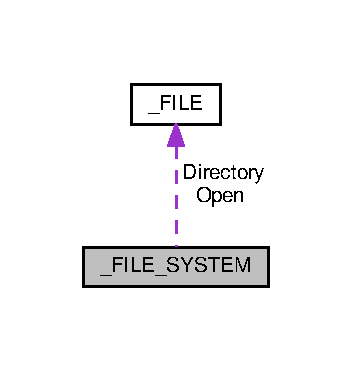
\includegraphics[width=169pt]{struct__FILE__SYSTEM__coll__graph}
\end{center}
\end{figure}
\subsection*{Data Fields}
\begin{DoxyCompactItemize}
\item 
char \hyperlink{struct__FILE__SYSTEM_a802d31f742c14deb2020c8bd6bcb4fdb}{Name} \mbox{[}8\mbox{]}
\item 
\hyperlink{vfs_8h_a175abb747ea3b78aa8da87355dcec473}{F\+I\+LE}($\ast$ \hyperlink{struct__FILE__SYSTEM_a96097c4b444cc7c7cd110f8f8c56ed55}{Directory} )(const char $\ast$Directory\+Name)
\item 
void($\ast$ \hyperlink{struct__FILE__SYSTEM_a5aa8d15979d91eec1ff97c4701594ff2}{Mount} )()
\item 
void($\ast$ \hyperlink{struct__FILE__SYSTEM_a24dcbcc9b82e7395aa6b15ef3e36413c}{Read} )(\hyperlink{vfs_8h_ad326c846895d1e06bc4c2228bf864968}{P\+F\+I\+LE} \hyperlink{structfile}{file}, unsigned char $\ast$Buffer, unsigned int Length)
\item 
void($\ast$ \hyperlink{struct__FILE__SYSTEM_a5595fce92d628028705b1ddd25d21e6f}{Close} )(\hyperlink{vfs_8h_ad326c846895d1e06bc4c2228bf864968}{P\+F\+I\+LE})
\item 
\hyperlink{vfs_8h_a175abb747ea3b78aa8da87355dcec473}{F\+I\+LE}($\ast$ \hyperlink{struct__FILE__SYSTEM_ae7183a7cfc938bbf1ed51aab2462b991}{Open} )(const char $\ast$File\+Name)
\end{DoxyCompactItemize}


\subsection{Detailed Description}


Definition at line 22 of file vfs.\+h.



\subsection{Field Documentation}
\index{\+\_\+\+F\+I\+L\+E\+\_\+\+S\+Y\+S\+T\+EM@{\+\_\+\+F\+I\+L\+E\+\_\+\+S\+Y\+S\+T\+EM}!Close@{Close}}
\index{Close@{Close}!\+\_\+\+F\+I\+L\+E\+\_\+\+S\+Y\+S\+T\+EM@{\+\_\+\+F\+I\+L\+E\+\_\+\+S\+Y\+S\+T\+EM}}
\subsubsection[{\texorpdfstring{Close}{Close}}]{\setlength{\rightskip}{0pt plus 5cm}void($\ast$ \+\_\+\+F\+I\+L\+E\+\_\+\+S\+Y\+S\+T\+E\+M\+::\+Close) ({\bf P\+F\+I\+LE})}\hypertarget{struct__FILE__SYSTEM_a5595fce92d628028705b1ddd25d21e6f}{}\label{struct__FILE__SYSTEM_a5595fce92d628028705b1ddd25d21e6f}


Definition at line 29 of file vfs.\+h.

\index{\+\_\+\+F\+I\+L\+E\+\_\+\+S\+Y\+S\+T\+EM@{\+\_\+\+F\+I\+L\+E\+\_\+\+S\+Y\+S\+T\+EM}!Directory@{Directory}}
\index{Directory@{Directory}!\+\_\+\+F\+I\+L\+E\+\_\+\+S\+Y\+S\+T\+EM@{\+\_\+\+F\+I\+L\+E\+\_\+\+S\+Y\+S\+T\+EM}}
\subsubsection[{\texorpdfstring{Directory}{Directory}}]{\setlength{\rightskip}{0pt plus 5cm}{\bf F\+I\+LE}($\ast$ \+\_\+\+F\+I\+L\+E\+\_\+\+S\+Y\+S\+T\+E\+M\+::\+Directory) (const char $\ast$Directory\+Name)}\hypertarget{struct__FILE__SYSTEM_a96097c4b444cc7c7cd110f8f8c56ed55}{}\label{struct__FILE__SYSTEM_a96097c4b444cc7c7cd110f8f8c56ed55}


Definition at line 26 of file vfs.\+h.

\index{\+\_\+\+F\+I\+L\+E\+\_\+\+S\+Y\+S\+T\+EM@{\+\_\+\+F\+I\+L\+E\+\_\+\+S\+Y\+S\+T\+EM}!Mount@{Mount}}
\index{Mount@{Mount}!\+\_\+\+F\+I\+L\+E\+\_\+\+S\+Y\+S\+T\+EM@{\+\_\+\+F\+I\+L\+E\+\_\+\+S\+Y\+S\+T\+EM}}
\subsubsection[{\texorpdfstring{Mount}{Mount}}]{\setlength{\rightskip}{0pt plus 5cm}void($\ast$ \+\_\+\+F\+I\+L\+E\+\_\+\+S\+Y\+S\+T\+E\+M\+::\+Mount) ()}\hypertarget{struct__FILE__SYSTEM_a5aa8d15979d91eec1ff97c4701594ff2}{}\label{struct__FILE__SYSTEM_a5aa8d15979d91eec1ff97c4701594ff2}


Definition at line 27 of file vfs.\+h.

\index{\+\_\+\+F\+I\+L\+E\+\_\+\+S\+Y\+S\+T\+EM@{\+\_\+\+F\+I\+L\+E\+\_\+\+S\+Y\+S\+T\+EM}!Name@{Name}}
\index{Name@{Name}!\+\_\+\+F\+I\+L\+E\+\_\+\+S\+Y\+S\+T\+EM@{\+\_\+\+F\+I\+L\+E\+\_\+\+S\+Y\+S\+T\+EM}}
\subsubsection[{\texorpdfstring{Name}{Name}}]{\setlength{\rightskip}{0pt plus 5cm}char \+\_\+\+F\+I\+L\+E\+\_\+\+S\+Y\+S\+T\+E\+M\+::\+Name\mbox{[}8\mbox{]}}\hypertarget{struct__FILE__SYSTEM_a802d31f742c14deb2020c8bd6bcb4fdb}{}\label{struct__FILE__SYSTEM_a802d31f742c14deb2020c8bd6bcb4fdb}


Definition at line 25 of file vfs.\+h.

\index{\+\_\+\+F\+I\+L\+E\+\_\+\+S\+Y\+S\+T\+EM@{\+\_\+\+F\+I\+L\+E\+\_\+\+S\+Y\+S\+T\+EM}!Open@{Open}}
\index{Open@{Open}!\+\_\+\+F\+I\+L\+E\+\_\+\+S\+Y\+S\+T\+EM@{\+\_\+\+F\+I\+L\+E\+\_\+\+S\+Y\+S\+T\+EM}}
\subsubsection[{\texorpdfstring{Open}{Open}}]{\setlength{\rightskip}{0pt plus 5cm}{\bf F\+I\+LE}($\ast$ \+\_\+\+F\+I\+L\+E\+\_\+\+S\+Y\+S\+T\+E\+M\+::\+Open) (const char $\ast$File\+Name)}\hypertarget{struct__FILE__SYSTEM_ae7183a7cfc938bbf1ed51aab2462b991}{}\label{struct__FILE__SYSTEM_ae7183a7cfc938bbf1ed51aab2462b991}


Definition at line 30 of file vfs.\+h.

\index{\+\_\+\+F\+I\+L\+E\+\_\+\+S\+Y\+S\+T\+EM@{\+\_\+\+F\+I\+L\+E\+\_\+\+S\+Y\+S\+T\+EM}!Read@{Read}}
\index{Read@{Read}!\+\_\+\+F\+I\+L\+E\+\_\+\+S\+Y\+S\+T\+EM@{\+\_\+\+F\+I\+L\+E\+\_\+\+S\+Y\+S\+T\+EM}}
\subsubsection[{\texorpdfstring{Read}{Read}}]{\setlength{\rightskip}{0pt plus 5cm}void($\ast$ \+\_\+\+F\+I\+L\+E\+\_\+\+S\+Y\+S\+T\+E\+M\+::\+Read) ({\bf P\+F\+I\+LE} {\bf file}, unsigned char $\ast$Buffer, unsigned int Length)}\hypertarget{struct__FILE__SYSTEM_a24dcbcc9b82e7395aa6b15ef3e36413c}{}\label{struct__FILE__SYSTEM_a24dcbcc9b82e7395aa6b15ef3e36413c}


Definition at line 28 of file vfs.\+h.



The documentation for this struct was generated from the following file\+:\begin{DoxyCompactItemize}
\item 
Experimental Edition/\+Source/vfs/\hyperlink{vfs_8h}{vfs.\+h}\end{DoxyCompactItemize}

\hypertarget{struct__MOUNT__INFO}{}\section{\+\_\+\+M\+O\+U\+N\+T\+\_\+\+I\+N\+FO Struct Reference}
\label{struct__MOUNT__INFO}\index{\+\_\+\+M\+O\+U\+N\+T\+\_\+\+I\+N\+FO@{\+\_\+\+M\+O\+U\+N\+T\+\_\+\+I\+N\+FO}}


{\ttfamily \#include $<$fat.\+h$>$}

\subsection*{Data Fields}
\begin{DoxyCompactItemize}
\item 
uint32\+\_\+t \hyperlink{struct__MOUNT__INFO_a0071bda2d72096f634544df8aacc3f32}{num\+Sectors}
\item 
uint32\+\_\+t \hyperlink{struct__MOUNT__INFO_a1aa114acfe01f60c8a85fe7a01d5c96d}{fat\+Offset}
\item 
uint32\+\_\+t \hyperlink{struct__MOUNT__INFO_afacdf709c99a10da00c6859acd935334}{num\+Root\+Entries}
\item 
uint32\+\_\+t \hyperlink{struct__MOUNT__INFO_aeccc0a73a2a1f4d2a55cd938461bcd45}{root\+Offset}
\item 
uint32\+\_\+t \hyperlink{struct__MOUNT__INFO_afe78a775d2d21ba728ffb7df951c26a2}{root\+Size}
\item 
uint32\+\_\+t \hyperlink{struct__MOUNT__INFO_a1c27dc07d9399da26e9836433514537e}{fat\+Size}
\item 
uint32\+\_\+t \hyperlink{struct__MOUNT__INFO_ade01217e0a9e58634a65b1279bbe95c6}{fat\+Entry\+Size}
\end{DoxyCompactItemize}


\subsection{Detailed Description}
Filesystem mount info 

Definition at line 28 of file fat.\+h.



\subsection{Field Documentation}
\index{\+\_\+\+M\+O\+U\+N\+T\+\_\+\+I\+N\+FO@{\+\_\+\+M\+O\+U\+N\+T\+\_\+\+I\+N\+FO}!fat\+Entry\+Size@{fat\+Entry\+Size}}
\index{fat\+Entry\+Size@{fat\+Entry\+Size}!\+\_\+\+M\+O\+U\+N\+T\+\_\+\+I\+N\+FO@{\+\_\+\+M\+O\+U\+N\+T\+\_\+\+I\+N\+FO}}
\subsubsection[{\texorpdfstring{fat\+Entry\+Size}{fatEntrySize}}]{\setlength{\rightskip}{0pt plus 5cm}uint32\+\_\+t \+\_\+\+M\+O\+U\+N\+T\+\_\+\+I\+N\+F\+O\+::fat\+Entry\+Size}\hypertarget{struct__MOUNT__INFO_ade01217e0a9e58634a65b1279bbe95c6}{}\label{struct__MOUNT__INFO_ade01217e0a9e58634a65b1279bbe95c6}


Definition at line 36 of file fat.\+h.

\index{\+\_\+\+M\+O\+U\+N\+T\+\_\+\+I\+N\+FO@{\+\_\+\+M\+O\+U\+N\+T\+\_\+\+I\+N\+FO}!fat\+Offset@{fat\+Offset}}
\index{fat\+Offset@{fat\+Offset}!\+\_\+\+M\+O\+U\+N\+T\+\_\+\+I\+N\+FO@{\+\_\+\+M\+O\+U\+N\+T\+\_\+\+I\+N\+FO}}
\subsubsection[{\texorpdfstring{fat\+Offset}{fatOffset}}]{\setlength{\rightskip}{0pt plus 5cm}uint32\+\_\+t \+\_\+\+M\+O\+U\+N\+T\+\_\+\+I\+N\+F\+O\+::fat\+Offset}\hypertarget{struct__MOUNT__INFO_a1aa114acfe01f60c8a85fe7a01d5c96d}{}\label{struct__MOUNT__INFO_a1aa114acfe01f60c8a85fe7a01d5c96d}


Definition at line 31 of file fat.\+h.

\index{\+\_\+\+M\+O\+U\+N\+T\+\_\+\+I\+N\+FO@{\+\_\+\+M\+O\+U\+N\+T\+\_\+\+I\+N\+FO}!fat\+Size@{fat\+Size}}
\index{fat\+Size@{fat\+Size}!\+\_\+\+M\+O\+U\+N\+T\+\_\+\+I\+N\+FO@{\+\_\+\+M\+O\+U\+N\+T\+\_\+\+I\+N\+FO}}
\subsubsection[{\texorpdfstring{fat\+Size}{fatSize}}]{\setlength{\rightskip}{0pt plus 5cm}uint32\+\_\+t \+\_\+\+M\+O\+U\+N\+T\+\_\+\+I\+N\+F\+O\+::fat\+Size}\hypertarget{struct__MOUNT__INFO_a1c27dc07d9399da26e9836433514537e}{}\label{struct__MOUNT__INFO_a1c27dc07d9399da26e9836433514537e}


Definition at line 35 of file fat.\+h.

\index{\+\_\+\+M\+O\+U\+N\+T\+\_\+\+I\+N\+FO@{\+\_\+\+M\+O\+U\+N\+T\+\_\+\+I\+N\+FO}!num\+Root\+Entries@{num\+Root\+Entries}}
\index{num\+Root\+Entries@{num\+Root\+Entries}!\+\_\+\+M\+O\+U\+N\+T\+\_\+\+I\+N\+FO@{\+\_\+\+M\+O\+U\+N\+T\+\_\+\+I\+N\+FO}}
\subsubsection[{\texorpdfstring{num\+Root\+Entries}{numRootEntries}}]{\setlength{\rightskip}{0pt plus 5cm}uint32\+\_\+t \+\_\+\+M\+O\+U\+N\+T\+\_\+\+I\+N\+F\+O\+::num\+Root\+Entries}\hypertarget{struct__MOUNT__INFO_afacdf709c99a10da00c6859acd935334}{}\label{struct__MOUNT__INFO_afacdf709c99a10da00c6859acd935334}


Definition at line 32 of file fat.\+h.

\index{\+\_\+\+M\+O\+U\+N\+T\+\_\+\+I\+N\+FO@{\+\_\+\+M\+O\+U\+N\+T\+\_\+\+I\+N\+FO}!num\+Sectors@{num\+Sectors}}
\index{num\+Sectors@{num\+Sectors}!\+\_\+\+M\+O\+U\+N\+T\+\_\+\+I\+N\+FO@{\+\_\+\+M\+O\+U\+N\+T\+\_\+\+I\+N\+FO}}
\subsubsection[{\texorpdfstring{num\+Sectors}{numSectors}}]{\setlength{\rightskip}{0pt plus 5cm}uint32\+\_\+t \+\_\+\+M\+O\+U\+N\+T\+\_\+\+I\+N\+F\+O\+::num\+Sectors}\hypertarget{struct__MOUNT__INFO_a0071bda2d72096f634544df8aacc3f32}{}\label{struct__MOUNT__INFO_a0071bda2d72096f634544df8aacc3f32}


Definition at line 30 of file fat.\+h.

\index{\+\_\+\+M\+O\+U\+N\+T\+\_\+\+I\+N\+FO@{\+\_\+\+M\+O\+U\+N\+T\+\_\+\+I\+N\+FO}!root\+Offset@{root\+Offset}}
\index{root\+Offset@{root\+Offset}!\+\_\+\+M\+O\+U\+N\+T\+\_\+\+I\+N\+FO@{\+\_\+\+M\+O\+U\+N\+T\+\_\+\+I\+N\+FO}}
\subsubsection[{\texorpdfstring{root\+Offset}{rootOffset}}]{\setlength{\rightskip}{0pt plus 5cm}uint32\+\_\+t \+\_\+\+M\+O\+U\+N\+T\+\_\+\+I\+N\+F\+O\+::root\+Offset}\hypertarget{struct__MOUNT__INFO_aeccc0a73a2a1f4d2a55cd938461bcd45}{}\label{struct__MOUNT__INFO_aeccc0a73a2a1f4d2a55cd938461bcd45}


Definition at line 33 of file fat.\+h.

\index{\+\_\+\+M\+O\+U\+N\+T\+\_\+\+I\+N\+FO@{\+\_\+\+M\+O\+U\+N\+T\+\_\+\+I\+N\+FO}!root\+Size@{root\+Size}}
\index{root\+Size@{root\+Size}!\+\_\+\+M\+O\+U\+N\+T\+\_\+\+I\+N\+FO@{\+\_\+\+M\+O\+U\+N\+T\+\_\+\+I\+N\+FO}}
\subsubsection[{\texorpdfstring{root\+Size}{rootSize}}]{\setlength{\rightskip}{0pt plus 5cm}uint32\+\_\+t \+\_\+\+M\+O\+U\+N\+T\+\_\+\+I\+N\+F\+O\+::root\+Size}\hypertarget{struct__MOUNT__INFO_afe78a775d2d21ba728ffb7df951c26a2}{}\label{struct__MOUNT__INFO_afe78a775d2d21ba728ffb7df951c26a2}


Definition at line 34 of file fat.\+h.



The documentation for this struct was generated from the following file\+:\begin{DoxyCompactItemize}
\item 
Experimental Edition/\+Source/vfs/\hyperlink{fat_8h}{fat.\+h}\end{DoxyCompactItemize}

\hypertarget{struct__PCI__CLASSCODETABLE}{}\section{\+\_\+\+P\+C\+I\+\_\+\+C\+L\+A\+S\+S\+C\+O\+D\+E\+T\+A\+B\+LE Struct Reference}
\label{struct__PCI__CLASSCODETABLE}\index{\+\_\+\+P\+C\+I\+\_\+\+C\+L\+A\+S\+S\+C\+O\+D\+E\+T\+A\+B\+LE@{\+\_\+\+P\+C\+I\+\_\+\+C\+L\+A\+S\+S\+C\+O\+D\+E\+T\+A\+B\+LE}}


{\ttfamily \#include $<$pci\+\_\+list.\+h$>$}

\subsection*{Data Fields}
\begin{DoxyCompactItemize}
\item 
unsigned char \hyperlink{struct__PCI__CLASSCODETABLE_a7a19960d9dbafb954b58363498d7f738}{Base\+Class}
\item 
unsigned char \hyperlink{struct__PCI__CLASSCODETABLE_afefd8246fde2dfbce05dd0bd79f2bf28}{Sub\+Class}
\item 
unsigned char \hyperlink{struct__PCI__CLASSCODETABLE_abc5ea223e3a634dfd00f40c5f3bede92}{Prog\+If}
\item 
const char $\ast$ \hyperlink{struct__PCI__CLASSCODETABLE_a6fd103aa14c2e4206a726ca1e60a0915}{Base\+Desc}
\item 
const char $\ast$ \hyperlink{struct__PCI__CLASSCODETABLE_aeab4f5eb6b728b0401d4a75fd497309c}{Sub\+Desc}
\item 
const char $\ast$ \hyperlink{struct__PCI__CLASSCODETABLE_a06501fb6914742547b7672ab9aaefae3}{Prog\+Desc}
\end{DoxyCompactItemize}


\subsection{Detailed Description}


Definition at line 6874 of file pci\+\_\+list.\+h.



\subsection{Field Documentation}
\index{\+\_\+\+P\+C\+I\+\_\+\+C\+L\+A\+S\+S\+C\+O\+D\+E\+T\+A\+B\+LE@{\+\_\+\+P\+C\+I\+\_\+\+C\+L\+A\+S\+S\+C\+O\+D\+E\+T\+A\+B\+LE}!Base\+Class@{Base\+Class}}
\index{Base\+Class@{Base\+Class}!\+\_\+\+P\+C\+I\+\_\+\+C\+L\+A\+S\+S\+C\+O\+D\+E\+T\+A\+B\+LE@{\+\_\+\+P\+C\+I\+\_\+\+C\+L\+A\+S\+S\+C\+O\+D\+E\+T\+A\+B\+LE}}
\subsubsection[{\texorpdfstring{Base\+Class}{BaseClass}}]{\setlength{\rightskip}{0pt plus 5cm}unsigned char \+\_\+\+P\+C\+I\+\_\+\+C\+L\+A\+S\+S\+C\+O\+D\+E\+T\+A\+B\+L\+E\+::\+Base\+Class}\hypertarget{struct__PCI__CLASSCODETABLE_a7a19960d9dbafb954b58363498d7f738}{}\label{struct__PCI__CLASSCODETABLE_a7a19960d9dbafb954b58363498d7f738}


Definition at line 6876 of file pci\+\_\+list.\+h.

\index{\+\_\+\+P\+C\+I\+\_\+\+C\+L\+A\+S\+S\+C\+O\+D\+E\+T\+A\+B\+LE@{\+\_\+\+P\+C\+I\+\_\+\+C\+L\+A\+S\+S\+C\+O\+D\+E\+T\+A\+B\+LE}!Base\+Desc@{Base\+Desc}}
\index{Base\+Desc@{Base\+Desc}!\+\_\+\+P\+C\+I\+\_\+\+C\+L\+A\+S\+S\+C\+O\+D\+E\+T\+A\+B\+LE@{\+\_\+\+P\+C\+I\+\_\+\+C\+L\+A\+S\+S\+C\+O\+D\+E\+T\+A\+B\+LE}}
\subsubsection[{\texorpdfstring{Base\+Desc}{BaseDesc}}]{\setlength{\rightskip}{0pt plus 5cm}const char$\ast$ \+\_\+\+P\+C\+I\+\_\+\+C\+L\+A\+S\+S\+C\+O\+D\+E\+T\+A\+B\+L\+E\+::\+Base\+Desc}\hypertarget{struct__PCI__CLASSCODETABLE_a6fd103aa14c2e4206a726ca1e60a0915}{}\label{struct__PCI__CLASSCODETABLE_a6fd103aa14c2e4206a726ca1e60a0915}


Definition at line 6879 of file pci\+\_\+list.\+h.

\index{\+\_\+\+P\+C\+I\+\_\+\+C\+L\+A\+S\+S\+C\+O\+D\+E\+T\+A\+B\+LE@{\+\_\+\+P\+C\+I\+\_\+\+C\+L\+A\+S\+S\+C\+O\+D\+E\+T\+A\+B\+LE}!Prog\+Desc@{Prog\+Desc}}
\index{Prog\+Desc@{Prog\+Desc}!\+\_\+\+P\+C\+I\+\_\+\+C\+L\+A\+S\+S\+C\+O\+D\+E\+T\+A\+B\+LE@{\+\_\+\+P\+C\+I\+\_\+\+C\+L\+A\+S\+S\+C\+O\+D\+E\+T\+A\+B\+LE}}
\subsubsection[{\texorpdfstring{Prog\+Desc}{ProgDesc}}]{\setlength{\rightskip}{0pt plus 5cm}const char$\ast$ \+\_\+\+P\+C\+I\+\_\+\+C\+L\+A\+S\+S\+C\+O\+D\+E\+T\+A\+B\+L\+E\+::\+Prog\+Desc}\hypertarget{struct__PCI__CLASSCODETABLE_a06501fb6914742547b7672ab9aaefae3}{}\label{struct__PCI__CLASSCODETABLE_a06501fb6914742547b7672ab9aaefae3}


Definition at line 6881 of file pci\+\_\+list.\+h.

\index{\+\_\+\+P\+C\+I\+\_\+\+C\+L\+A\+S\+S\+C\+O\+D\+E\+T\+A\+B\+LE@{\+\_\+\+P\+C\+I\+\_\+\+C\+L\+A\+S\+S\+C\+O\+D\+E\+T\+A\+B\+LE}!Prog\+If@{Prog\+If}}
\index{Prog\+If@{Prog\+If}!\+\_\+\+P\+C\+I\+\_\+\+C\+L\+A\+S\+S\+C\+O\+D\+E\+T\+A\+B\+LE@{\+\_\+\+P\+C\+I\+\_\+\+C\+L\+A\+S\+S\+C\+O\+D\+E\+T\+A\+B\+LE}}
\subsubsection[{\texorpdfstring{Prog\+If}{ProgIf}}]{\setlength{\rightskip}{0pt plus 5cm}unsigned char \+\_\+\+P\+C\+I\+\_\+\+C\+L\+A\+S\+S\+C\+O\+D\+E\+T\+A\+B\+L\+E\+::\+Prog\+If}\hypertarget{struct__PCI__CLASSCODETABLE_abc5ea223e3a634dfd00f40c5f3bede92}{}\label{struct__PCI__CLASSCODETABLE_abc5ea223e3a634dfd00f40c5f3bede92}


Definition at line 6878 of file pci\+\_\+list.\+h.

\index{\+\_\+\+P\+C\+I\+\_\+\+C\+L\+A\+S\+S\+C\+O\+D\+E\+T\+A\+B\+LE@{\+\_\+\+P\+C\+I\+\_\+\+C\+L\+A\+S\+S\+C\+O\+D\+E\+T\+A\+B\+LE}!Sub\+Class@{Sub\+Class}}
\index{Sub\+Class@{Sub\+Class}!\+\_\+\+P\+C\+I\+\_\+\+C\+L\+A\+S\+S\+C\+O\+D\+E\+T\+A\+B\+LE@{\+\_\+\+P\+C\+I\+\_\+\+C\+L\+A\+S\+S\+C\+O\+D\+E\+T\+A\+B\+LE}}
\subsubsection[{\texorpdfstring{Sub\+Class}{SubClass}}]{\setlength{\rightskip}{0pt plus 5cm}unsigned char \+\_\+\+P\+C\+I\+\_\+\+C\+L\+A\+S\+S\+C\+O\+D\+E\+T\+A\+B\+L\+E\+::\+Sub\+Class}\hypertarget{struct__PCI__CLASSCODETABLE_afefd8246fde2dfbce05dd0bd79f2bf28}{}\label{struct__PCI__CLASSCODETABLE_afefd8246fde2dfbce05dd0bd79f2bf28}


Definition at line 6877 of file pci\+\_\+list.\+h.

\index{\+\_\+\+P\+C\+I\+\_\+\+C\+L\+A\+S\+S\+C\+O\+D\+E\+T\+A\+B\+LE@{\+\_\+\+P\+C\+I\+\_\+\+C\+L\+A\+S\+S\+C\+O\+D\+E\+T\+A\+B\+LE}!Sub\+Desc@{Sub\+Desc}}
\index{Sub\+Desc@{Sub\+Desc}!\+\_\+\+P\+C\+I\+\_\+\+C\+L\+A\+S\+S\+C\+O\+D\+E\+T\+A\+B\+LE@{\+\_\+\+P\+C\+I\+\_\+\+C\+L\+A\+S\+S\+C\+O\+D\+E\+T\+A\+B\+LE}}
\subsubsection[{\texorpdfstring{Sub\+Desc}{SubDesc}}]{\setlength{\rightskip}{0pt plus 5cm}const char$\ast$ \+\_\+\+P\+C\+I\+\_\+\+C\+L\+A\+S\+S\+C\+O\+D\+E\+T\+A\+B\+L\+E\+::\+Sub\+Desc}\hypertarget{struct__PCI__CLASSCODETABLE_aeab4f5eb6b728b0401d4a75fd497309c}{}\label{struct__PCI__CLASSCODETABLE_aeab4f5eb6b728b0401d4a75fd497309c}


Definition at line 6880 of file pci\+\_\+list.\+h.



The documentation for this struct was generated from the following file\+:\begin{DoxyCompactItemize}
\item 
Experimental Edition/\+Source/\+Drivers/\+P\+C\+I/\hyperlink{pci__list_8h}{pci\+\_\+list.\+h}\end{DoxyCompactItemize}

\hypertarget{struct__PCI__DEVTABLE}{}\section{\+\_\+\+P\+C\+I\+\_\+\+D\+E\+V\+T\+A\+B\+LE Struct Reference}
\label{struct__PCI__DEVTABLE}\index{\+\_\+\+P\+C\+I\+\_\+\+D\+E\+V\+T\+A\+B\+LE@{\+\_\+\+P\+C\+I\+\_\+\+D\+E\+V\+T\+A\+B\+LE}}


{\ttfamily \#include $<$pci\+\_\+list.\+h$>$}

\subsection*{Data Fields}
\begin{DoxyCompactItemize}
\item 
unsigned short \hyperlink{struct__PCI__DEVTABLE_acab5aacfc4cdfc1f3c71e9f835c52a61}{Ven\+Id}
\item 
unsigned short \hyperlink{struct__PCI__DEVTABLE_a843e7019bff5cda0c58a061814dfdbe6}{Dev\+Id}
\item 
const char $\ast$ \hyperlink{struct__PCI__DEVTABLE_afe06a83864adc5504ea8eb4644f6f194}{Chip}
\item 
const char $\ast$ \hyperlink{struct__PCI__DEVTABLE_aa93c23c253df7ff6365b332220f447ec}{Chip\+Desc}
\end{DoxyCompactItemize}


\subsection{Detailed Description}


Definition at line 1520 of file pci\+\_\+list.\+h.



\subsection{Field Documentation}
\index{\+\_\+\+P\+C\+I\+\_\+\+D\+E\+V\+T\+A\+B\+LE@{\+\_\+\+P\+C\+I\+\_\+\+D\+E\+V\+T\+A\+B\+LE}!Chip@{Chip}}
\index{Chip@{Chip}!\+\_\+\+P\+C\+I\+\_\+\+D\+E\+V\+T\+A\+B\+LE@{\+\_\+\+P\+C\+I\+\_\+\+D\+E\+V\+T\+A\+B\+LE}}
\subsubsection[{\texorpdfstring{Chip}{Chip}}]{\setlength{\rightskip}{0pt plus 5cm}const char$\ast$ \+\_\+\+P\+C\+I\+\_\+\+D\+E\+V\+T\+A\+B\+L\+E\+::\+Chip}\hypertarget{struct__PCI__DEVTABLE_afe06a83864adc5504ea8eb4644f6f194}{}\label{struct__PCI__DEVTABLE_afe06a83864adc5504ea8eb4644f6f194}


Definition at line 1524 of file pci\+\_\+list.\+h.

\index{\+\_\+\+P\+C\+I\+\_\+\+D\+E\+V\+T\+A\+B\+LE@{\+\_\+\+P\+C\+I\+\_\+\+D\+E\+V\+T\+A\+B\+LE}!Chip\+Desc@{Chip\+Desc}}
\index{Chip\+Desc@{Chip\+Desc}!\+\_\+\+P\+C\+I\+\_\+\+D\+E\+V\+T\+A\+B\+LE@{\+\_\+\+P\+C\+I\+\_\+\+D\+E\+V\+T\+A\+B\+LE}}
\subsubsection[{\texorpdfstring{Chip\+Desc}{ChipDesc}}]{\setlength{\rightskip}{0pt plus 5cm}const char$\ast$ \+\_\+\+P\+C\+I\+\_\+\+D\+E\+V\+T\+A\+B\+L\+E\+::\+Chip\+Desc}\hypertarget{struct__PCI__DEVTABLE_aa93c23c253df7ff6365b332220f447ec}{}\label{struct__PCI__DEVTABLE_aa93c23c253df7ff6365b332220f447ec}


Definition at line 1525 of file pci\+\_\+list.\+h.

\index{\+\_\+\+P\+C\+I\+\_\+\+D\+E\+V\+T\+A\+B\+LE@{\+\_\+\+P\+C\+I\+\_\+\+D\+E\+V\+T\+A\+B\+LE}!Dev\+Id@{Dev\+Id}}
\index{Dev\+Id@{Dev\+Id}!\+\_\+\+P\+C\+I\+\_\+\+D\+E\+V\+T\+A\+B\+LE@{\+\_\+\+P\+C\+I\+\_\+\+D\+E\+V\+T\+A\+B\+LE}}
\subsubsection[{\texorpdfstring{Dev\+Id}{DevId}}]{\setlength{\rightskip}{0pt plus 5cm}unsigned short \+\_\+\+P\+C\+I\+\_\+\+D\+E\+V\+T\+A\+B\+L\+E\+::\+Dev\+Id}\hypertarget{struct__PCI__DEVTABLE_a843e7019bff5cda0c58a061814dfdbe6}{}\label{struct__PCI__DEVTABLE_a843e7019bff5cda0c58a061814dfdbe6}


Definition at line 1523 of file pci\+\_\+list.\+h.

\index{\+\_\+\+P\+C\+I\+\_\+\+D\+E\+V\+T\+A\+B\+LE@{\+\_\+\+P\+C\+I\+\_\+\+D\+E\+V\+T\+A\+B\+LE}!Ven\+Id@{Ven\+Id}}
\index{Ven\+Id@{Ven\+Id}!\+\_\+\+P\+C\+I\+\_\+\+D\+E\+V\+T\+A\+B\+LE@{\+\_\+\+P\+C\+I\+\_\+\+D\+E\+V\+T\+A\+B\+LE}}
\subsubsection[{\texorpdfstring{Ven\+Id}{VenId}}]{\setlength{\rightskip}{0pt plus 5cm}unsigned short \+\_\+\+P\+C\+I\+\_\+\+D\+E\+V\+T\+A\+B\+L\+E\+::\+Ven\+Id}\hypertarget{struct__PCI__DEVTABLE_acab5aacfc4cdfc1f3c71e9f835c52a61}{}\label{struct__PCI__DEVTABLE_acab5aacfc4cdfc1f3c71e9f835c52a61}


Definition at line 1522 of file pci\+\_\+list.\+h.



The documentation for this struct was generated from the following file\+:\begin{DoxyCompactItemize}
\item 
Experimental Edition/\+Source/\+Drivers/\+P\+C\+I/\hyperlink{pci__list_8h}{pci\+\_\+list.\+h}\end{DoxyCompactItemize}

\hypertarget{struct__PCI__VENTABLE}{}\section{\+\_\+\+P\+C\+I\+\_\+\+V\+E\+N\+T\+A\+B\+LE Struct Reference}
\label{struct__PCI__VENTABLE}\index{\+\_\+\+P\+C\+I\+\_\+\+V\+E\+N\+T\+A\+B\+LE@{\+\_\+\+P\+C\+I\+\_\+\+V\+E\+N\+T\+A\+B\+LE}}


{\ttfamily \#include $<$pci\+\_\+list.\+h$>$}

\subsection*{Data Fields}
\begin{DoxyCompactItemize}
\item 
unsigned short \hyperlink{struct__PCI__VENTABLE_a8df580b1447df15ebe8a128b8225e710}{Ven\+Id}
\item 
const char $\ast$ \hyperlink{struct__PCI__VENTABLE_a37c44257d4237ef312626d97ef3a5fa5}{Ven\+Short}
\item 
const char $\ast$ \hyperlink{struct__PCI__VENTABLE_aad91ea393afe64b533c1ad399f12baf2}{Ven\+Full}
\end{DoxyCompactItemize}


\subsection{Detailed Description}


Definition at line 7 of file pci\+\_\+list.\+h.



\subsection{Field Documentation}
\index{\+\_\+\+P\+C\+I\+\_\+\+V\+E\+N\+T\+A\+B\+LE@{\+\_\+\+P\+C\+I\+\_\+\+V\+E\+N\+T\+A\+B\+LE}!Ven\+Full@{Ven\+Full}}
\index{Ven\+Full@{Ven\+Full}!\+\_\+\+P\+C\+I\+\_\+\+V\+E\+N\+T\+A\+B\+LE@{\+\_\+\+P\+C\+I\+\_\+\+V\+E\+N\+T\+A\+B\+LE}}
\subsubsection[{\texorpdfstring{Ven\+Full}{VenFull}}]{\setlength{\rightskip}{0pt plus 5cm}const char$\ast$ \+\_\+\+P\+C\+I\+\_\+\+V\+E\+N\+T\+A\+B\+L\+E\+::\+Ven\+Full}\hypertarget{struct__PCI__VENTABLE_aad91ea393afe64b533c1ad399f12baf2}{}\label{struct__PCI__VENTABLE_aad91ea393afe64b533c1ad399f12baf2}


Definition at line 11 of file pci\+\_\+list.\+h.

\index{\+\_\+\+P\+C\+I\+\_\+\+V\+E\+N\+T\+A\+B\+LE@{\+\_\+\+P\+C\+I\+\_\+\+V\+E\+N\+T\+A\+B\+LE}!Ven\+Id@{Ven\+Id}}
\index{Ven\+Id@{Ven\+Id}!\+\_\+\+P\+C\+I\+\_\+\+V\+E\+N\+T\+A\+B\+LE@{\+\_\+\+P\+C\+I\+\_\+\+V\+E\+N\+T\+A\+B\+LE}}
\subsubsection[{\texorpdfstring{Ven\+Id}{VenId}}]{\setlength{\rightskip}{0pt plus 5cm}unsigned short \+\_\+\+P\+C\+I\+\_\+\+V\+E\+N\+T\+A\+B\+L\+E\+::\+Ven\+Id}\hypertarget{struct__PCI__VENTABLE_a8df580b1447df15ebe8a128b8225e710}{}\label{struct__PCI__VENTABLE_a8df580b1447df15ebe8a128b8225e710}


Definition at line 9 of file pci\+\_\+list.\+h.

\index{\+\_\+\+P\+C\+I\+\_\+\+V\+E\+N\+T\+A\+B\+LE@{\+\_\+\+P\+C\+I\+\_\+\+V\+E\+N\+T\+A\+B\+LE}!Ven\+Short@{Ven\+Short}}
\index{Ven\+Short@{Ven\+Short}!\+\_\+\+P\+C\+I\+\_\+\+V\+E\+N\+T\+A\+B\+LE@{\+\_\+\+P\+C\+I\+\_\+\+V\+E\+N\+T\+A\+B\+LE}}
\subsubsection[{\texorpdfstring{Ven\+Short}{VenShort}}]{\setlength{\rightskip}{0pt plus 5cm}const char$\ast$ \+\_\+\+P\+C\+I\+\_\+\+V\+E\+N\+T\+A\+B\+L\+E\+::\+Ven\+Short}\hypertarget{struct__PCI__VENTABLE_a37c44257d4237ef312626d97ef3a5fa5}{}\label{struct__PCI__VENTABLE_a37c44257d4237ef312626d97ef3a5fa5}


Definition at line 10 of file pci\+\_\+list.\+h.



The documentation for this struct was generated from the following file\+:\begin{DoxyCompactItemize}
\item 
Experimental Edition/\+Source/\+Drivers/\+P\+C\+I/\hyperlink{pci__list_8h}{pci\+\_\+list.\+h}\end{DoxyCompactItemize}

\hypertarget{struct__PciDevice}{}\section{\+\_\+\+Pci\+Device Struct Reference}
\label{struct__PciDevice}\index{\+\_\+\+Pci\+Device@{\+\_\+\+Pci\+Device}}


{\ttfamily \#include $<$P\+C\+I.\+h$>$}



Collaboration diagram for \+\_\+\+Pci\+Device\+:
\nopagebreak
\begin{figure}[H]
\begin{center}
\leavevmode
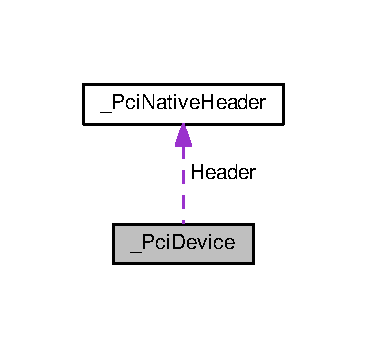
\includegraphics[width=176pt]{struct__PciDevice__coll__graph}
\end{center}
\end{figure}
\subsection*{Data Fields}
\begin{DoxyCompactItemize}
\item 
uint32\+\_\+t \hyperlink{struct__PciDevice_a57d861d58ee386f1fe1d8820c1e409c5}{Type}
\item 
\hyperlink{common_8h_a61350201bbcea1180bb1160bd09b717f}{s32int} \hyperlink{struct__PciDevice_ac99e17b6dde217c76aeec72883f4d1e7}{Bus}
\item 
uint32\+\_\+t \hyperlink{struct__PciDevice_abab1111099256cd120062a3c01d56f75}{Device}
\item 
uint32\+\_\+t \hyperlink{struct__PciDevice_ac8b9939eac2f6edaf3372d22871554e7}{Function}
\item 
\hyperlink{PCI_8h_a478d1e5507b733431433bfe46bc1d465}{Pci\+Native\+Header\+\_\+t} $\ast$ \hyperlink{struct__PciDevice_a308d9d7234decbd3802735bf0a83e156}{Header}
\item 
void $\ast$ \hyperlink{struct__PciDevice_ac46c4ff9140c0d3c4609f3cf53cea0e6}{Parent}
\item 
void $\ast$ \hyperlink{struct__PciDevice_adf56e308e389296a7a4612b048d906f7}{Children}
\end{DoxyCompactItemize}


\subsection{Detailed Description}


Definition at line 135 of file P\+C\+I.\+h.



\subsection{Field Documentation}
\index{\+\_\+\+Pci\+Device@{\+\_\+\+Pci\+Device}!Bus@{Bus}}
\index{Bus@{Bus}!\+\_\+\+Pci\+Device@{\+\_\+\+Pci\+Device}}
\subsubsection[{\texorpdfstring{Bus}{Bus}}]{\setlength{\rightskip}{0pt plus 5cm}{\bf s32int} \+\_\+\+Pci\+Device\+::\+Bus}\hypertarget{struct__PciDevice_ac99e17b6dde217c76aeec72883f4d1e7}{}\label{struct__PciDevice_ac99e17b6dde217c76aeec72883f4d1e7}


Definition at line 141 of file P\+C\+I.\+h.

\index{\+\_\+\+Pci\+Device@{\+\_\+\+Pci\+Device}!Children@{Children}}
\index{Children@{Children}!\+\_\+\+Pci\+Device@{\+\_\+\+Pci\+Device}}
\subsubsection[{\texorpdfstring{Children}{Children}}]{\setlength{\rightskip}{0pt plus 5cm}void$\ast$ \+\_\+\+Pci\+Device\+::\+Children}\hypertarget{struct__PciDevice_adf56e308e389296a7a4612b048d906f7}{}\label{struct__PciDevice_adf56e308e389296a7a4612b048d906f7}


Definition at line 150 of file P\+C\+I.\+h.

\index{\+\_\+\+Pci\+Device@{\+\_\+\+Pci\+Device}!Device@{Device}}
\index{Device@{Device}!\+\_\+\+Pci\+Device@{\+\_\+\+Pci\+Device}}
\subsubsection[{\texorpdfstring{Device}{Device}}]{\setlength{\rightskip}{0pt plus 5cm}uint32\+\_\+t \+\_\+\+Pci\+Device\+::\+Device}\hypertarget{struct__PciDevice_abab1111099256cd120062a3c01d56f75}{}\label{struct__PciDevice_abab1111099256cd120062a3c01d56f75}


Definition at line 142 of file P\+C\+I.\+h.

\index{\+\_\+\+Pci\+Device@{\+\_\+\+Pci\+Device}!Function@{Function}}
\index{Function@{Function}!\+\_\+\+Pci\+Device@{\+\_\+\+Pci\+Device}}
\subsubsection[{\texorpdfstring{Function}{Function}}]{\setlength{\rightskip}{0pt plus 5cm}uint32\+\_\+t \+\_\+\+Pci\+Device\+::\+Function}\hypertarget{struct__PciDevice_ac8b9939eac2f6edaf3372d22871554e7}{}\label{struct__PciDevice_ac8b9939eac2f6edaf3372d22871554e7}


Definition at line 143 of file P\+C\+I.\+h.

\index{\+\_\+\+Pci\+Device@{\+\_\+\+Pci\+Device}!Header@{Header}}
\index{Header@{Header}!\+\_\+\+Pci\+Device@{\+\_\+\+Pci\+Device}}
\subsubsection[{\texorpdfstring{Header}{Header}}]{\setlength{\rightskip}{0pt plus 5cm}{\bf Pci\+Native\+Header\+\_\+t}$\ast$ \+\_\+\+Pci\+Device\+::\+Header}\hypertarget{struct__PciDevice_a308d9d7234decbd3802735bf0a83e156}{}\label{struct__PciDevice_a308d9d7234decbd3802735bf0a83e156}


Definition at line 146 of file P\+C\+I.\+h.

\index{\+\_\+\+Pci\+Device@{\+\_\+\+Pci\+Device}!Parent@{Parent}}
\index{Parent@{Parent}!\+\_\+\+Pci\+Device@{\+\_\+\+Pci\+Device}}
\subsubsection[{\texorpdfstring{Parent}{Parent}}]{\setlength{\rightskip}{0pt plus 5cm}void$\ast$ \+\_\+\+Pci\+Device\+::\+Parent}\hypertarget{struct__PciDevice_ac46c4ff9140c0d3c4609f3cf53cea0e6}{}\label{struct__PciDevice_ac46c4ff9140c0d3c4609f3cf53cea0e6}


Definition at line 149 of file P\+C\+I.\+h.

\index{\+\_\+\+Pci\+Device@{\+\_\+\+Pci\+Device}!Type@{Type}}
\index{Type@{Type}!\+\_\+\+Pci\+Device@{\+\_\+\+Pci\+Device}}
\subsubsection[{\texorpdfstring{Type}{Type}}]{\setlength{\rightskip}{0pt plus 5cm}uint32\+\_\+t \+\_\+\+Pci\+Device\+::\+Type}\hypertarget{struct__PciDevice_a57d861d58ee386f1fe1d8820c1e409c5}{}\label{struct__PciDevice_a57d861d58ee386f1fe1d8820c1e409c5}


Definition at line 138 of file P\+C\+I.\+h.



The documentation for this struct was generated from the following file\+:\begin{DoxyCompactItemize}
\item 
Experimental Edition/\+Source/\+Drivers/\+P\+C\+I/\hyperlink{PCI_8h}{P\+C\+I.\+h}\end{DoxyCompactItemize}

\hypertarget{struct__PciNativeHeader}{}\section{\+\_\+\+Pci\+Native\+Header Struct Reference}
\label{struct__PciNativeHeader}\index{\+\_\+\+Pci\+Native\+Header@{\+\_\+\+Pci\+Native\+Header}}


{\ttfamily \#include $<$P\+C\+I.\+h$>$}

\subsection*{Data Fields}
\begin{DoxyCompactItemize}
\item 
uint16\+\_\+t \hyperlink{struct__PciNativeHeader_acc809b557a84fbe99da19b442210e6a1}{Vendor\+Id}
\item 
uint16\+\_\+t \hyperlink{struct__PciNativeHeader_a4cb00b77b64768cc8754c3b5938a09ea}{Device\+Id}
\item 
uint16\+\_\+t \hyperlink{struct__PciNativeHeader_a81ce29fa9d9c0c10e6dd3694171a4c26}{Command}
\item 
uint16\+\_\+t \hyperlink{struct__PciNativeHeader_a8e4bcdfb2744454f91bae6ee68ce0a44}{Status}
\item 
uint8\+\_\+t \hyperlink{struct__PciNativeHeader_a655b55f4aec8aa162568754a43e61117}{Revision}
\item 
uint8\+\_\+t \hyperlink{struct__PciNativeHeader_ada9dcea6b70e8eb30bfc652af3e90cb1}{Interface}
\item 
uint8\+\_\+t \hyperlink{struct__PciNativeHeader_a988d996c402af2ac9a89b86d409815b5}{Subclass}
\item 
uint8\+\_\+t \hyperlink{struct__PciNativeHeader_a2feb2dca74bf9ff2af1e08ebbb310241}{Class}
\item 
uint8\+\_\+t \hyperlink{struct__PciNativeHeader_a2a524801b4961a6ef1ed8df9fd658621}{Cache\+Line\+Size}
\item 
uint8\+\_\+t \hyperlink{struct__PciNativeHeader_a730fa76240530058c4833de2b1fd6925}{Latency\+Timer}
\item 
uint8\+\_\+t \hyperlink{struct__PciNativeHeader_a3eadff3dde49511e8771e19769964e23}{Header\+Type}
\item 
uint8\+\_\+t \hyperlink{struct__PciNativeHeader_a57e75ff47ecc5d366d176a20e4023931}{Bist}
\item 
uint32\+\_\+t \hyperlink{struct__PciNativeHeader_a5ea1ceacaf1539a1f43d418cb35d5ae0}{Bar0}
\item 
uint32\+\_\+t \hyperlink{struct__PciNativeHeader_aa9af6e2520f693035c7db1b08532bbac}{Bar1}
\item 
uint32\+\_\+t \hyperlink{struct__PciNativeHeader_aefeefb8bb0d4d2c8c9d699b146472abb}{Bar2}
\item 
uint32\+\_\+t \hyperlink{struct__PciNativeHeader_a7db6363b61b19d6a52ef679b22f560cb}{Bar3}
\item 
uint32\+\_\+t \hyperlink{struct__PciNativeHeader_a1fdd80a61e6b295ebbe6ba26483c9e2a}{Bar4}
\item 
uint32\+\_\+t \hyperlink{struct__PciNativeHeader_aa18626af4b1e61cb290c6c8fb2e8a895}{Bar5}
\item 
uint32\+\_\+t \hyperlink{struct__PciNativeHeader_a229757839cd81fceafa182234d1ec930}{Cardbus\+C\+I\+S\+Ptr}
\item 
uint16\+\_\+t \hyperlink{struct__PciNativeHeader_aded2bf4a3ea0efc410cf091ae736ae7e}{Sub\+System\+Vendor\+Id}
\item 
uint16\+\_\+t \hyperlink{struct__PciNativeHeader_a890fa8d2edfa526899a3c547f0fff6ee}{Sub\+System\+Id}
\item 
uint32\+\_\+t \hyperlink{struct__PciNativeHeader_aed3842654fc63d6948453582c90c7897}{Expansion\+Rom\+Base\+Addr}
\item 
uint32\+\_\+t \hyperlink{struct__PciNativeHeader_ac6854a65538b035591311219fc52b973}{Reserved0}
\item 
uint32\+\_\+t \hyperlink{struct__PciNativeHeader_a34aafe4c4f8bcc909d2fad92f04c1c6c}{Reserved1}
\item 
uint8\+\_\+t \hyperlink{struct__PciNativeHeader_a5d3013816300453589fefcd1ed9c5cee}{Interrupt\+Line}
\item 
uint8\+\_\+t \hyperlink{struct__PciNativeHeader_aa1d37e93fd702731475ccc0775b048d8}{Interrupt\+Pin}
\item 
uint8\+\_\+t \hyperlink{struct__PciNativeHeader_a5c11c079111e6235bd01540b9affdb8b}{Min\+Grant}
\item 
uint8\+\_\+t \hyperlink{struct__PciNativeHeader_af9a63a39fe2cd333b78e77b0c8a9652e}{Max\+Latency}
\end{DoxyCompactItemize}


\subsection{Detailed Description}


Definition at line 77 of file P\+C\+I.\+h.



\subsection{Field Documentation}
\index{\+\_\+\+Pci\+Native\+Header@{\+\_\+\+Pci\+Native\+Header}!Bar0@{Bar0}}
\index{Bar0@{Bar0}!\+\_\+\+Pci\+Native\+Header@{\+\_\+\+Pci\+Native\+Header}}
\subsubsection[{\texorpdfstring{Bar0}{Bar0}}]{\setlength{\rightskip}{0pt plus 5cm}uint32\+\_\+t \+\_\+\+Pci\+Native\+Header\+::\+Bar0}\hypertarget{struct__PciNativeHeader_a5ea1ceacaf1539a1f43d418cb35d5ae0}{}\label{struct__PciNativeHeader_a5ea1ceacaf1539a1f43d418cb35d5ae0}


Definition at line 100 of file P\+C\+I.\+h.

\index{\+\_\+\+Pci\+Native\+Header@{\+\_\+\+Pci\+Native\+Header}!Bar1@{Bar1}}
\index{Bar1@{Bar1}!\+\_\+\+Pci\+Native\+Header@{\+\_\+\+Pci\+Native\+Header}}
\subsubsection[{\texorpdfstring{Bar1}{Bar1}}]{\setlength{\rightskip}{0pt plus 5cm}uint32\+\_\+t \+\_\+\+Pci\+Native\+Header\+::\+Bar1}\hypertarget{struct__PciNativeHeader_aa9af6e2520f693035c7db1b08532bbac}{}\label{struct__PciNativeHeader_aa9af6e2520f693035c7db1b08532bbac}


Definition at line 102 of file P\+C\+I.\+h.

\index{\+\_\+\+Pci\+Native\+Header@{\+\_\+\+Pci\+Native\+Header}!Bar2@{Bar2}}
\index{Bar2@{Bar2}!\+\_\+\+Pci\+Native\+Header@{\+\_\+\+Pci\+Native\+Header}}
\subsubsection[{\texorpdfstring{Bar2}{Bar2}}]{\setlength{\rightskip}{0pt plus 5cm}uint32\+\_\+t \+\_\+\+Pci\+Native\+Header\+::\+Bar2}\hypertarget{struct__PciNativeHeader_aefeefb8bb0d4d2c8c9d699b146472abb}{}\label{struct__PciNativeHeader_aefeefb8bb0d4d2c8c9d699b146472abb}


Definition at line 104 of file P\+C\+I.\+h.

\index{\+\_\+\+Pci\+Native\+Header@{\+\_\+\+Pci\+Native\+Header}!Bar3@{Bar3}}
\index{Bar3@{Bar3}!\+\_\+\+Pci\+Native\+Header@{\+\_\+\+Pci\+Native\+Header}}
\subsubsection[{\texorpdfstring{Bar3}{Bar3}}]{\setlength{\rightskip}{0pt plus 5cm}uint32\+\_\+t \+\_\+\+Pci\+Native\+Header\+::\+Bar3}\hypertarget{struct__PciNativeHeader_a7db6363b61b19d6a52ef679b22f560cb}{}\label{struct__PciNativeHeader_a7db6363b61b19d6a52ef679b22f560cb}


Definition at line 106 of file P\+C\+I.\+h.

\index{\+\_\+\+Pci\+Native\+Header@{\+\_\+\+Pci\+Native\+Header}!Bar4@{Bar4}}
\index{Bar4@{Bar4}!\+\_\+\+Pci\+Native\+Header@{\+\_\+\+Pci\+Native\+Header}}
\subsubsection[{\texorpdfstring{Bar4}{Bar4}}]{\setlength{\rightskip}{0pt plus 5cm}uint32\+\_\+t \+\_\+\+Pci\+Native\+Header\+::\+Bar4}\hypertarget{struct__PciNativeHeader_a1fdd80a61e6b295ebbe6ba26483c9e2a}{}\label{struct__PciNativeHeader_a1fdd80a61e6b295ebbe6ba26483c9e2a}


Definition at line 108 of file P\+C\+I.\+h.

\index{\+\_\+\+Pci\+Native\+Header@{\+\_\+\+Pci\+Native\+Header}!Bar5@{Bar5}}
\index{Bar5@{Bar5}!\+\_\+\+Pci\+Native\+Header@{\+\_\+\+Pci\+Native\+Header}}
\subsubsection[{\texorpdfstring{Bar5}{Bar5}}]{\setlength{\rightskip}{0pt plus 5cm}uint32\+\_\+t \+\_\+\+Pci\+Native\+Header\+::\+Bar5}\hypertarget{struct__PciNativeHeader_aa18626af4b1e61cb290c6c8fb2e8a895}{}\label{struct__PciNativeHeader_aa18626af4b1e61cb290c6c8fb2e8a895}


Definition at line 110 of file P\+C\+I.\+h.

\index{\+\_\+\+Pci\+Native\+Header@{\+\_\+\+Pci\+Native\+Header}!Bist@{Bist}}
\index{Bist@{Bist}!\+\_\+\+Pci\+Native\+Header@{\+\_\+\+Pci\+Native\+Header}}
\subsubsection[{\texorpdfstring{Bist}{Bist}}]{\setlength{\rightskip}{0pt plus 5cm}uint8\+\_\+t \+\_\+\+Pci\+Native\+Header\+::\+Bist}\hypertarget{struct__PciNativeHeader_a57e75ff47ecc5d366d176a20e4023931}{}\label{struct__PciNativeHeader_a57e75ff47ecc5d366d176a20e4023931}


Definition at line 97 of file P\+C\+I.\+h.

\index{\+\_\+\+Pci\+Native\+Header@{\+\_\+\+Pci\+Native\+Header}!Cache\+Line\+Size@{Cache\+Line\+Size}}
\index{Cache\+Line\+Size@{Cache\+Line\+Size}!\+\_\+\+Pci\+Native\+Header@{\+\_\+\+Pci\+Native\+Header}}
\subsubsection[{\texorpdfstring{Cache\+Line\+Size}{CacheLineSize}}]{\setlength{\rightskip}{0pt plus 5cm}uint8\+\_\+t \+\_\+\+Pci\+Native\+Header\+::\+Cache\+Line\+Size}\hypertarget{struct__PciNativeHeader_a2a524801b4961a6ef1ed8df9fd658621}{}\label{struct__PciNativeHeader_a2a524801b4961a6ef1ed8df9fd658621}


Definition at line 94 of file P\+C\+I.\+h.

\index{\+\_\+\+Pci\+Native\+Header@{\+\_\+\+Pci\+Native\+Header}!Cardbus\+C\+I\+S\+Ptr@{Cardbus\+C\+I\+S\+Ptr}}
\index{Cardbus\+C\+I\+S\+Ptr@{Cardbus\+C\+I\+S\+Ptr}!\+\_\+\+Pci\+Native\+Header@{\+\_\+\+Pci\+Native\+Header}}
\subsubsection[{\texorpdfstring{Cardbus\+C\+I\+S\+Ptr}{CardbusCISPtr}}]{\setlength{\rightskip}{0pt plus 5cm}uint32\+\_\+t \+\_\+\+Pci\+Native\+Header\+::\+Cardbus\+C\+I\+S\+Ptr}\hypertarget{struct__PciNativeHeader_a229757839cd81fceafa182234d1ec930}{}\label{struct__PciNativeHeader_a229757839cd81fceafa182234d1ec930}


Definition at line 113 of file P\+C\+I.\+h.

\index{\+\_\+\+Pci\+Native\+Header@{\+\_\+\+Pci\+Native\+Header}!Class@{Class}}
\index{Class@{Class}!\+\_\+\+Pci\+Native\+Header@{\+\_\+\+Pci\+Native\+Header}}
\subsubsection[{\texorpdfstring{Class}{Class}}]{\setlength{\rightskip}{0pt plus 5cm}uint8\+\_\+t \+\_\+\+Pci\+Native\+Header\+::\+Class}\hypertarget{struct__PciNativeHeader_a2feb2dca74bf9ff2af1e08ebbb310241}{}\label{struct__PciNativeHeader_a2feb2dca74bf9ff2af1e08ebbb310241}


Definition at line 91 of file P\+C\+I.\+h.

\index{\+\_\+\+Pci\+Native\+Header@{\+\_\+\+Pci\+Native\+Header}!Command@{Command}}
\index{Command@{Command}!\+\_\+\+Pci\+Native\+Header@{\+\_\+\+Pci\+Native\+Header}}
\subsubsection[{\texorpdfstring{Command}{Command}}]{\setlength{\rightskip}{0pt plus 5cm}uint16\+\_\+t \+\_\+\+Pci\+Native\+Header\+::\+Command}\hypertarget{struct__PciNativeHeader_a81ce29fa9d9c0c10e6dd3694171a4c26}{}\label{struct__PciNativeHeader_a81ce29fa9d9c0c10e6dd3694171a4c26}


Definition at line 84 of file P\+C\+I.\+h.

\index{\+\_\+\+Pci\+Native\+Header@{\+\_\+\+Pci\+Native\+Header}!Device\+Id@{Device\+Id}}
\index{Device\+Id@{Device\+Id}!\+\_\+\+Pci\+Native\+Header@{\+\_\+\+Pci\+Native\+Header}}
\subsubsection[{\texorpdfstring{Device\+Id}{DeviceId}}]{\setlength{\rightskip}{0pt plus 5cm}uint16\+\_\+t \+\_\+\+Pci\+Native\+Header\+::\+Device\+Id}\hypertarget{struct__PciNativeHeader_a4cb00b77b64768cc8754c3b5938a09ea}{}\label{struct__PciNativeHeader_a4cb00b77b64768cc8754c3b5938a09ea}


Definition at line 81 of file P\+C\+I.\+h.

\index{\+\_\+\+Pci\+Native\+Header@{\+\_\+\+Pci\+Native\+Header}!Expansion\+Rom\+Base\+Addr@{Expansion\+Rom\+Base\+Addr}}
\index{Expansion\+Rom\+Base\+Addr@{Expansion\+Rom\+Base\+Addr}!\+\_\+\+Pci\+Native\+Header@{\+\_\+\+Pci\+Native\+Header}}
\subsubsection[{\texorpdfstring{Expansion\+Rom\+Base\+Addr}{ExpansionRomBaseAddr}}]{\setlength{\rightskip}{0pt plus 5cm}uint32\+\_\+t \+\_\+\+Pci\+Native\+Header\+::\+Expansion\+Rom\+Base\+Addr}\hypertarget{struct__PciNativeHeader_aed3842654fc63d6948453582c90c7897}{}\label{struct__PciNativeHeader_aed3842654fc63d6948453582c90c7897}


Definition at line 119 of file P\+C\+I.\+h.

\index{\+\_\+\+Pci\+Native\+Header@{\+\_\+\+Pci\+Native\+Header}!Header\+Type@{Header\+Type}}
\index{Header\+Type@{Header\+Type}!\+\_\+\+Pci\+Native\+Header@{\+\_\+\+Pci\+Native\+Header}}
\subsubsection[{\texorpdfstring{Header\+Type}{HeaderType}}]{\setlength{\rightskip}{0pt plus 5cm}uint8\+\_\+t \+\_\+\+Pci\+Native\+Header\+::\+Header\+Type}\hypertarget{struct__PciNativeHeader_a3eadff3dde49511e8771e19769964e23}{}\label{struct__PciNativeHeader_a3eadff3dde49511e8771e19769964e23}


Definition at line 96 of file P\+C\+I.\+h.

\index{\+\_\+\+Pci\+Native\+Header@{\+\_\+\+Pci\+Native\+Header}!Interface@{Interface}}
\index{Interface@{Interface}!\+\_\+\+Pci\+Native\+Header@{\+\_\+\+Pci\+Native\+Header}}
\subsubsection[{\texorpdfstring{Interface}{Interface}}]{\setlength{\rightskip}{0pt plus 5cm}uint8\+\_\+t \+\_\+\+Pci\+Native\+Header\+::\+Interface}\hypertarget{struct__PciNativeHeader_ada9dcea6b70e8eb30bfc652af3e90cb1}{}\label{struct__PciNativeHeader_ada9dcea6b70e8eb30bfc652af3e90cb1}


Definition at line 89 of file P\+C\+I.\+h.

\index{\+\_\+\+Pci\+Native\+Header@{\+\_\+\+Pci\+Native\+Header}!Interrupt\+Line@{Interrupt\+Line}}
\index{Interrupt\+Line@{Interrupt\+Line}!\+\_\+\+Pci\+Native\+Header@{\+\_\+\+Pci\+Native\+Header}}
\subsubsection[{\texorpdfstring{Interrupt\+Line}{InterruptLine}}]{\setlength{\rightskip}{0pt plus 5cm}uint8\+\_\+t \+\_\+\+Pci\+Native\+Header\+::\+Interrupt\+Line}\hypertarget{struct__PciNativeHeader_a5d3013816300453589fefcd1ed9c5cee}{}\label{struct__PciNativeHeader_a5d3013816300453589fefcd1ed9c5cee}


Definition at line 128 of file P\+C\+I.\+h.

\index{\+\_\+\+Pci\+Native\+Header@{\+\_\+\+Pci\+Native\+Header}!Interrupt\+Pin@{Interrupt\+Pin}}
\index{Interrupt\+Pin@{Interrupt\+Pin}!\+\_\+\+Pci\+Native\+Header@{\+\_\+\+Pci\+Native\+Header}}
\subsubsection[{\texorpdfstring{Interrupt\+Pin}{InterruptPin}}]{\setlength{\rightskip}{0pt plus 5cm}uint8\+\_\+t \+\_\+\+Pci\+Native\+Header\+::\+Interrupt\+Pin}\hypertarget{struct__PciNativeHeader_aa1d37e93fd702731475ccc0775b048d8}{}\label{struct__PciNativeHeader_aa1d37e93fd702731475ccc0775b048d8}


Definition at line 129 of file P\+C\+I.\+h.

\index{\+\_\+\+Pci\+Native\+Header@{\+\_\+\+Pci\+Native\+Header}!Latency\+Timer@{Latency\+Timer}}
\index{Latency\+Timer@{Latency\+Timer}!\+\_\+\+Pci\+Native\+Header@{\+\_\+\+Pci\+Native\+Header}}
\subsubsection[{\texorpdfstring{Latency\+Timer}{LatencyTimer}}]{\setlength{\rightskip}{0pt plus 5cm}uint8\+\_\+t \+\_\+\+Pci\+Native\+Header\+::\+Latency\+Timer}\hypertarget{struct__PciNativeHeader_a730fa76240530058c4833de2b1fd6925}{}\label{struct__PciNativeHeader_a730fa76240530058c4833de2b1fd6925}


Definition at line 95 of file P\+C\+I.\+h.

\index{\+\_\+\+Pci\+Native\+Header@{\+\_\+\+Pci\+Native\+Header}!Max\+Latency@{Max\+Latency}}
\index{Max\+Latency@{Max\+Latency}!\+\_\+\+Pci\+Native\+Header@{\+\_\+\+Pci\+Native\+Header}}
\subsubsection[{\texorpdfstring{Max\+Latency}{MaxLatency}}]{\setlength{\rightskip}{0pt plus 5cm}uint8\+\_\+t \+\_\+\+Pci\+Native\+Header\+::\+Max\+Latency}\hypertarget{struct__PciNativeHeader_af9a63a39fe2cd333b78e77b0c8a9652e}{}\label{struct__PciNativeHeader_af9a63a39fe2cd333b78e77b0c8a9652e}


Definition at line 131 of file P\+C\+I.\+h.

\index{\+\_\+\+Pci\+Native\+Header@{\+\_\+\+Pci\+Native\+Header}!Min\+Grant@{Min\+Grant}}
\index{Min\+Grant@{Min\+Grant}!\+\_\+\+Pci\+Native\+Header@{\+\_\+\+Pci\+Native\+Header}}
\subsubsection[{\texorpdfstring{Min\+Grant}{MinGrant}}]{\setlength{\rightskip}{0pt plus 5cm}uint8\+\_\+t \+\_\+\+Pci\+Native\+Header\+::\+Min\+Grant}\hypertarget{struct__PciNativeHeader_a5c11c079111e6235bd01540b9affdb8b}{}\label{struct__PciNativeHeader_a5c11c079111e6235bd01540b9affdb8b}


Definition at line 130 of file P\+C\+I.\+h.

\index{\+\_\+\+Pci\+Native\+Header@{\+\_\+\+Pci\+Native\+Header}!Reserved0@{Reserved0}}
\index{Reserved0@{Reserved0}!\+\_\+\+Pci\+Native\+Header@{\+\_\+\+Pci\+Native\+Header}}
\subsubsection[{\texorpdfstring{Reserved0}{Reserved0}}]{\setlength{\rightskip}{0pt plus 5cm}uint32\+\_\+t \+\_\+\+Pci\+Native\+Header\+::\+Reserved0}\hypertarget{struct__PciNativeHeader_ac6854a65538b035591311219fc52b973}{}\label{struct__PciNativeHeader_ac6854a65538b035591311219fc52b973}


Definition at line 122 of file P\+C\+I.\+h.

\index{\+\_\+\+Pci\+Native\+Header@{\+\_\+\+Pci\+Native\+Header}!Reserved1@{Reserved1}}
\index{Reserved1@{Reserved1}!\+\_\+\+Pci\+Native\+Header@{\+\_\+\+Pci\+Native\+Header}}
\subsubsection[{\texorpdfstring{Reserved1}{Reserved1}}]{\setlength{\rightskip}{0pt plus 5cm}uint32\+\_\+t \+\_\+\+Pci\+Native\+Header\+::\+Reserved1}\hypertarget{struct__PciNativeHeader_a34aafe4c4f8bcc909d2fad92f04c1c6c}{}\label{struct__PciNativeHeader_a34aafe4c4f8bcc909d2fad92f04c1c6c}


Definition at line 125 of file P\+C\+I.\+h.

\index{\+\_\+\+Pci\+Native\+Header@{\+\_\+\+Pci\+Native\+Header}!Revision@{Revision}}
\index{Revision@{Revision}!\+\_\+\+Pci\+Native\+Header@{\+\_\+\+Pci\+Native\+Header}}
\subsubsection[{\texorpdfstring{Revision}{Revision}}]{\setlength{\rightskip}{0pt plus 5cm}uint8\+\_\+t \+\_\+\+Pci\+Native\+Header\+::\+Revision}\hypertarget{struct__PciNativeHeader_a655b55f4aec8aa162568754a43e61117}{}\label{struct__PciNativeHeader_a655b55f4aec8aa162568754a43e61117}


Definition at line 88 of file P\+C\+I.\+h.

\index{\+\_\+\+Pci\+Native\+Header@{\+\_\+\+Pci\+Native\+Header}!Status@{Status}}
\index{Status@{Status}!\+\_\+\+Pci\+Native\+Header@{\+\_\+\+Pci\+Native\+Header}}
\subsubsection[{\texorpdfstring{Status}{Status}}]{\setlength{\rightskip}{0pt plus 5cm}uint16\+\_\+t \+\_\+\+Pci\+Native\+Header\+::\+Status}\hypertarget{struct__PciNativeHeader_a8e4bcdfb2744454f91bae6ee68ce0a44}{}\label{struct__PciNativeHeader_a8e4bcdfb2744454f91bae6ee68ce0a44}


Definition at line 85 of file P\+C\+I.\+h.

\index{\+\_\+\+Pci\+Native\+Header@{\+\_\+\+Pci\+Native\+Header}!Subclass@{Subclass}}
\index{Subclass@{Subclass}!\+\_\+\+Pci\+Native\+Header@{\+\_\+\+Pci\+Native\+Header}}
\subsubsection[{\texorpdfstring{Subclass}{Subclass}}]{\setlength{\rightskip}{0pt plus 5cm}uint8\+\_\+t \+\_\+\+Pci\+Native\+Header\+::\+Subclass}\hypertarget{struct__PciNativeHeader_a988d996c402af2ac9a89b86d409815b5}{}\label{struct__PciNativeHeader_a988d996c402af2ac9a89b86d409815b5}


Definition at line 90 of file P\+C\+I.\+h.

\index{\+\_\+\+Pci\+Native\+Header@{\+\_\+\+Pci\+Native\+Header}!Sub\+System\+Id@{Sub\+System\+Id}}
\index{Sub\+System\+Id@{Sub\+System\+Id}!\+\_\+\+Pci\+Native\+Header@{\+\_\+\+Pci\+Native\+Header}}
\subsubsection[{\texorpdfstring{Sub\+System\+Id}{SubSystemId}}]{\setlength{\rightskip}{0pt plus 5cm}uint16\+\_\+t \+\_\+\+Pci\+Native\+Header\+::\+Sub\+System\+Id}\hypertarget{struct__PciNativeHeader_a890fa8d2edfa526899a3c547f0fff6ee}{}\label{struct__PciNativeHeader_a890fa8d2edfa526899a3c547f0fff6ee}


Definition at line 116 of file P\+C\+I.\+h.

\index{\+\_\+\+Pci\+Native\+Header@{\+\_\+\+Pci\+Native\+Header}!Sub\+System\+Vendor\+Id@{Sub\+System\+Vendor\+Id}}
\index{Sub\+System\+Vendor\+Id@{Sub\+System\+Vendor\+Id}!\+\_\+\+Pci\+Native\+Header@{\+\_\+\+Pci\+Native\+Header}}
\subsubsection[{\texorpdfstring{Sub\+System\+Vendor\+Id}{SubSystemVendorId}}]{\setlength{\rightskip}{0pt plus 5cm}uint16\+\_\+t \+\_\+\+Pci\+Native\+Header\+::\+Sub\+System\+Vendor\+Id}\hypertarget{struct__PciNativeHeader_aded2bf4a3ea0efc410cf091ae736ae7e}{}\label{struct__PciNativeHeader_aded2bf4a3ea0efc410cf091ae736ae7e}


Definition at line 115 of file P\+C\+I.\+h.

\index{\+\_\+\+Pci\+Native\+Header@{\+\_\+\+Pci\+Native\+Header}!Vendor\+Id@{Vendor\+Id}}
\index{Vendor\+Id@{Vendor\+Id}!\+\_\+\+Pci\+Native\+Header@{\+\_\+\+Pci\+Native\+Header}}
\subsubsection[{\texorpdfstring{Vendor\+Id}{VendorId}}]{\setlength{\rightskip}{0pt plus 5cm}uint16\+\_\+t \+\_\+\+Pci\+Native\+Header\+::\+Vendor\+Id}\hypertarget{struct__PciNativeHeader_acc809b557a84fbe99da19b442210e6a1}{}\label{struct__PciNativeHeader_acc809b557a84fbe99da19b442210e6a1}


Definition at line 80 of file P\+C\+I.\+h.



The documentation for this struct was generated from the following file\+:\begin{DoxyCompactItemize}
\item 
Experimental Edition/\+Source/\+Drivers/\+P\+C\+I/\hyperlink{PCI_8h}{P\+C\+I.\+h}\end{DoxyCompactItemize}

\hypertarget{structahci__prdt}{}\section{ahci\+\_\+prdt Struct Reference}
\label{structahci__prdt}\index{ahci\+\_\+prdt@{ahci\+\_\+prdt}}


{\ttfamily \#include $<$ahci.\+h$>$}

\subsection*{Data Fields}
\begin{DoxyCompactItemize}
\item 
uint32\+\_\+t \hyperlink{structahci__prdt_a9425b0f49c1db09325d54e3ac89f484c}{phys\+\_\+addr}
\item 
uint32\+\_\+t \hyperlink{structahci__prdt_ad0746001774899f0a76d979e224ba575}{something}
\item 
uint32\+\_\+t \hyperlink{structahci__prdt_aa4716f5df6a9c798985643286a4260a4}{reserved}
\item 
uint32\+\_\+t \hyperlink{structahci__prdt_a91317b1c7fe022ac12b35f36835fc82f}{len}
\end{DoxyCompactItemize}


\subsection{Detailed Description}


Definition at line 649 of file ahci.\+h.



\subsection{Field Documentation}
\index{ahci\+\_\+prdt@{ahci\+\_\+prdt}!len@{len}}
\index{len@{len}!ahci\+\_\+prdt@{ahci\+\_\+prdt}}
\subsubsection[{\texorpdfstring{len}{len}}]{\setlength{\rightskip}{0pt plus 5cm}uint32\+\_\+t ahci\+\_\+prdt\+::len}\hypertarget{structahci__prdt_a91317b1c7fe022ac12b35f36835fc82f}{}\label{structahci__prdt_a91317b1c7fe022ac12b35f36835fc82f}


Definition at line 654 of file ahci.\+h.

\index{ahci\+\_\+prdt@{ahci\+\_\+prdt}!phys\+\_\+addr@{phys\+\_\+addr}}
\index{phys\+\_\+addr@{phys\+\_\+addr}!ahci\+\_\+prdt@{ahci\+\_\+prdt}}
\subsubsection[{\texorpdfstring{phys\+\_\+addr}{phys_addr}}]{\setlength{\rightskip}{0pt plus 5cm}uint32\+\_\+t ahci\+\_\+prdt\+::phys\+\_\+addr}\hypertarget{structahci__prdt_a9425b0f49c1db09325d54e3ac89f484c}{}\label{structahci__prdt_a9425b0f49c1db09325d54e3ac89f484c}


Definition at line 651 of file ahci.\+h.

\index{ahci\+\_\+prdt@{ahci\+\_\+prdt}!reserved@{reserved}}
\index{reserved@{reserved}!ahci\+\_\+prdt@{ahci\+\_\+prdt}}
\subsubsection[{\texorpdfstring{reserved}{reserved}}]{\setlength{\rightskip}{0pt plus 5cm}uint32\+\_\+t ahci\+\_\+prdt\+::reserved}\hypertarget{structahci__prdt_aa4716f5df6a9c798985643286a4260a4}{}\label{structahci__prdt_aa4716f5df6a9c798985643286a4260a4}


Definition at line 653 of file ahci.\+h.

\index{ahci\+\_\+prdt@{ahci\+\_\+prdt}!something@{something}}
\index{something@{something}!ahci\+\_\+prdt@{ahci\+\_\+prdt}}
\subsubsection[{\texorpdfstring{something}{something}}]{\setlength{\rightskip}{0pt plus 5cm}uint32\+\_\+t ahci\+\_\+prdt\+::something}\hypertarget{structahci__prdt_ad0746001774899f0a76d979e224ba575}{}\label{structahci__prdt_ad0746001774899f0a76d979e224ba575}


Definition at line 652 of file ahci.\+h.



The documentation for this struct was generated from the following file\+:\begin{DoxyCompactItemize}
\item 
Experimental Edition/\+Source/\+Drivers/\+A\+H\+C\+I/\hyperlink{ahci_8h}{ahci.\+h}\end{DoxyCompactItemize}

\hypertarget{structAhciCommandHeader}{}\section{Ahci\+Command\+Header Struct Reference}
\label{structAhciCommandHeader}\index{Ahci\+Command\+Header@{Ahci\+Command\+Header}}


{\ttfamily \#include $<$ahci.\+h$>$}

\subsection*{Data Fields}
\begin{DoxyCompactItemize}
\item 
uint32\+\_\+t \hyperlink{structAhciCommandHeader_a262106d4145e1d9fb8574b141dfac452}{opts}
\item 
uint32\+\_\+t \hyperlink{structAhciCommandHeader_aaeb18d131010effc76b3f40a9c06851a}{status}
\item 
uint32\+\_\+t \hyperlink{structAhciCommandHeader_a9a0af3edb5552ae52039b7f6f9f74abc}{tbl\+\_\+addr}
\item 
uint32\+\_\+t \hyperlink{structAhciCommandHeader_a92b0f59b1f834422312f180691c76a2e}{tbl\+\_\+addr\+\_\+hi}
\item 
uint32\+\_\+t \hyperlink{structAhciCommandHeader_ab20b140ede005b7d17cc59d961ba2976}{reserved} \mbox{[}4\mbox{]}
\end{DoxyCompactItemize}


\subsection{Detailed Description}


Definition at line 166 of file ahci.\+h.



\subsection{Field Documentation}
\index{Ahci\+Command\+Header@{Ahci\+Command\+Header}!opts@{opts}}
\index{opts@{opts}!Ahci\+Command\+Header@{Ahci\+Command\+Header}}
\subsubsection[{\texorpdfstring{opts}{opts}}]{\setlength{\rightskip}{0pt plus 5cm}uint32\+\_\+t Ahci\+Command\+Header\+::opts}\hypertarget{structAhciCommandHeader_a262106d4145e1d9fb8574b141dfac452}{}\label{structAhciCommandHeader_a262106d4145e1d9fb8574b141dfac452}


Definition at line 167 of file ahci.\+h.

\index{Ahci\+Command\+Header@{Ahci\+Command\+Header}!reserved@{reserved}}
\index{reserved@{reserved}!Ahci\+Command\+Header@{Ahci\+Command\+Header}}
\subsubsection[{\texorpdfstring{reserved}{reserved}}]{\setlength{\rightskip}{0pt plus 5cm}uint32\+\_\+t Ahci\+Command\+Header\+::reserved\mbox{[}4\mbox{]}}\hypertarget{structAhciCommandHeader_ab20b140ede005b7d17cc59d961ba2976}{}\label{structAhciCommandHeader_ab20b140ede005b7d17cc59d961ba2976}


Definition at line 171 of file ahci.\+h.

\index{Ahci\+Command\+Header@{Ahci\+Command\+Header}!status@{status}}
\index{status@{status}!Ahci\+Command\+Header@{Ahci\+Command\+Header}}
\subsubsection[{\texorpdfstring{status}{status}}]{\setlength{\rightskip}{0pt plus 5cm}uint32\+\_\+t Ahci\+Command\+Header\+::status}\hypertarget{structAhciCommandHeader_aaeb18d131010effc76b3f40a9c06851a}{}\label{structAhciCommandHeader_aaeb18d131010effc76b3f40a9c06851a}


Definition at line 168 of file ahci.\+h.

\index{Ahci\+Command\+Header@{Ahci\+Command\+Header}!tbl\+\_\+addr@{tbl\+\_\+addr}}
\index{tbl\+\_\+addr@{tbl\+\_\+addr}!Ahci\+Command\+Header@{Ahci\+Command\+Header}}
\subsubsection[{\texorpdfstring{tbl\+\_\+addr}{tbl_addr}}]{\setlength{\rightskip}{0pt plus 5cm}uint32\+\_\+t Ahci\+Command\+Header\+::tbl\+\_\+addr}\hypertarget{structAhciCommandHeader_a9a0af3edb5552ae52039b7f6f9f74abc}{}\label{structAhciCommandHeader_a9a0af3edb5552ae52039b7f6f9f74abc}


Definition at line 169 of file ahci.\+h.

\index{Ahci\+Command\+Header@{Ahci\+Command\+Header}!tbl\+\_\+addr\+\_\+hi@{tbl\+\_\+addr\+\_\+hi}}
\index{tbl\+\_\+addr\+\_\+hi@{tbl\+\_\+addr\+\_\+hi}!Ahci\+Command\+Header@{Ahci\+Command\+Header}}
\subsubsection[{\texorpdfstring{tbl\+\_\+addr\+\_\+hi}{tbl_addr_hi}}]{\setlength{\rightskip}{0pt plus 5cm}uint32\+\_\+t Ahci\+Command\+Header\+::tbl\+\_\+addr\+\_\+hi}\hypertarget{structAhciCommandHeader_a92b0f59b1f834422312f180691c76a2e}{}\label{structAhciCommandHeader_a92b0f59b1f834422312f180691c76a2e}


Definition at line 170 of file ahci.\+h.



The documentation for this struct was generated from the following file\+:\begin{DoxyCompactItemize}
\item 
Experimental Edition/\+Source/\+Drivers/\+A\+H\+C\+I/\hyperlink{ahci_8h}{ahci.\+h}\end{DoxyCompactItemize}

\hypertarget{structAhciIoPort}{}\section{Ahci\+Io\+Port Struct Reference}
\label{structAhciIoPort}\index{Ahci\+Io\+Port@{Ahci\+Io\+Port}}


{\ttfamily \#include $<$ahci.\+h$>$}



Collaboration diagram for Ahci\+Io\+Port\+:
\nopagebreak
\begin{figure}[H]
\begin{center}
\leavevmode
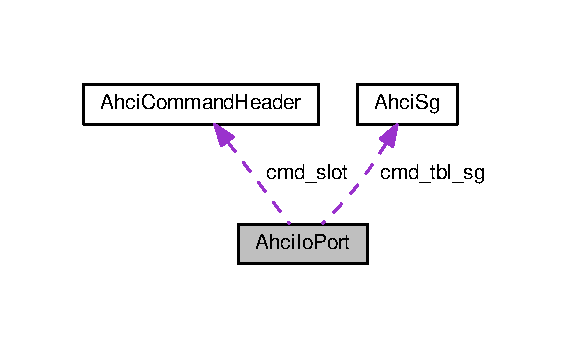
\includegraphics[width=274pt]{structAhciIoPort__coll__graph}
\end{center}
\end{figure}
\subsection*{Data Fields}
\begin{DoxyCompactItemize}
\item 
void $\ast$ \hyperlink{structAhciIoPort_ae62df7029d120c6efa10deebede2b1e9}{cmd\+\_\+addr}
\item 
void $\ast$ \hyperlink{structAhciIoPort_a5f15bb2db00d1bcfee213b59a0477452}{scr\+\_\+addr}
\item 
void $\ast$ \hyperlink{structAhciIoPort_a160a4ec60fb246c73a3c23a47aff0426}{port\+\_\+mmio}
\item 
\hyperlink{structAhciCommandHeader}{Ahci\+Command\+Header} $\ast$ \hyperlink{structAhciIoPort_a428f4de0af81ffd4be8a83cc763bfd27}{cmd\+\_\+slot}
\item 
\hyperlink{structAhciSg}{Ahci\+Sg} $\ast$ \hyperlink{structAhciIoPort_a71965bd481c51a76e529ec68b863acd5}{cmd\+\_\+tbl\+\_\+sg}
\item 
void $\ast$ \hyperlink{structAhciIoPort_a8768362980d0f4bee31bdce784b28c07}{cmd\+\_\+tbl}
\item 
void $\ast$ \hyperlink{structAhciIoPort_a0b1d803da9f594706b01b2edba108253}{rx\+\_\+fis}
\item 
int \hyperlink{structAhciIoPort_a011f1e42e32e23744a6395a0c9b8bb21}{index}
\end{DoxyCompactItemize}


\subsection{Detailed Description}


Definition at line 181 of file ahci.\+h.



\subsection{Field Documentation}
\index{Ahci\+Io\+Port@{Ahci\+Io\+Port}!cmd\+\_\+addr@{cmd\+\_\+addr}}
\index{cmd\+\_\+addr@{cmd\+\_\+addr}!Ahci\+Io\+Port@{Ahci\+Io\+Port}}
\subsubsection[{\texorpdfstring{cmd\+\_\+addr}{cmd_addr}}]{\setlength{\rightskip}{0pt plus 5cm}void$\ast$ Ahci\+Io\+Port\+::cmd\+\_\+addr}\hypertarget{structAhciIoPort_ae62df7029d120c6efa10deebede2b1e9}{}\label{structAhciIoPort_ae62df7029d120c6efa10deebede2b1e9}


Definition at line 182 of file ahci.\+h.

\index{Ahci\+Io\+Port@{Ahci\+Io\+Port}!cmd\+\_\+slot@{cmd\+\_\+slot}}
\index{cmd\+\_\+slot@{cmd\+\_\+slot}!Ahci\+Io\+Port@{Ahci\+Io\+Port}}
\subsubsection[{\texorpdfstring{cmd\+\_\+slot}{cmd_slot}}]{\setlength{\rightskip}{0pt plus 5cm}{\bf Ahci\+Command\+Header}$\ast$ Ahci\+Io\+Port\+::cmd\+\_\+slot}\hypertarget{structAhciIoPort_a428f4de0af81ffd4be8a83cc763bfd27}{}\label{structAhciIoPort_a428f4de0af81ffd4be8a83cc763bfd27}


Definition at line 185 of file ahci.\+h.

\index{Ahci\+Io\+Port@{Ahci\+Io\+Port}!cmd\+\_\+tbl@{cmd\+\_\+tbl}}
\index{cmd\+\_\+tbl@{cmd\+\_\+tbl}!Ahci\+Io\+Port@{Ahci\+Io\+Port}}
\subsubsection[{\texorpdfstring{cmd\+\_\+tbl}{cmd_tbl}}]{\setlength{\rightskip}{0pt plus 5cm}void$\ast$ Ahci\+Io\+Port\+::cmd\+\_\+tbl}\hypertarget{structAhciIoPort_a8768362980d0f4bee31bdce784b28c07}{}\label{structAhciIoPort_a8768362980d0f4bee31bdce784b28c07}


Definition at line 187 of file ahci.\+h.

\index{Ahci\+Io\+Port@{Ahci\+Io\+Port}!cmd\+\_\+tbl\+\_\+sg@{cmd\+\_\+tbl\+\_\+sg}}
\index{cmd\+\_\+tbl\+\_\+sg@{cmd\+\_\+tbl\+\_\+sg}!Ahci\+Io\+Port@{Ahci\+Io\+Port}}
\subsubsection[{\texorpdfstring{cmd\+\_\+tbl\+\_\+sg}{cmd_tbl_sg}}]{\setlength{\rightskip}{0pt plus 5cm}{\bf Ahci\+Sg}$\ast$ Ahci\+Io\+Port\+::cmd\+\_\+tbl\+\_\+sg}\hypertarget{structAhciIoPort_a71965bd481c51a76e529ec68b863acd5}{}\label{structAhciIoPort_a71965bd481c51a76e529ec68b863acd5}


Definition at line 186 of file ahci.\+h.

\index{Ahci\+Io\+Port@{Ahci\+Io\+Port}!index@{index}}
\index{index@{index}!Ahci\+Io\+Port@{Ahci\+Io\+Port}}
\subsubsection[{\texorpdfstring{index}{index}}]{\setlength{\rightskip}{0pt plus 5cm}int Ahci\+Io\+Port\+::index}\hypertarget{structAhciIoPort_a011f1e42e32e23744a6395a0c9b8bb21}{}\label{structAhciIoPort_a011f1e42e32e23744a6395a0c9b8bb21}


Definition at line 189 of file ahci.\+h.

\index{Ahci\+Io\+Port@{Ahci\+Io\+Port}!port\+\_\+mmio@{port\+\_\+mmio}}
\index{port\+\_\+mmio@{port\+\_\+mmio}!Ahci\+Io\+Port@{Ahci\+Io\+Port}}
\subsubsection[{\texorpdfstring{port\+\_\+mmio}{port_mmio}}]{\setlength{\rightskip}{0pt plus 5cm}void$\ast$ Ahci\+Io\+Port\+::port\+\_\+mmio}\hypertarget{structAhciIoPort_a160a4ec60fb246c73a3c23a47aff0426}{}\label{structAhciIoPort_a160a4ec60fb246c73a3c23a47aff0426}


Definition at line 184 of file ahci.\+h.

\index{Ahci\+Io\+Port@{Ahci\+Io\+Port}!rx\+\_\+fis@{rx\+\_\+fis}}
\index{rx\+\_\+fis@{rx\+\_\+fis}!Ahci\+Io\+Port@{Ahci\+Io\+Port}}
\subsubsection[{\texorpdfstring{rx\+\_\+fis}{rx_fis}}]{\setlength{\rightskip}{0pt plus 5cm}void$\ast$ Ahci\+Io\+Port\+::rx\+\_\+fis}\hypertarget{structAhciIoPort_a0b1d803da9f594706b01b2edba108253}{}\label{structAhciIoPort_a0b1d803da9f594706b01b2edba108253}


Definition at line 188 of file ahci.\+h.

\index{Ahci\+Io\+Port@{Ahci\+Io\+Port}!scr\+\_\+addr@{scr\+\_\+addr}}
\index{scr\+\_\+addr@{scr\+\_\+addr}!Ahci\+Io\+Port@{Ahci\+Io\+Port}}
\subsubsection[{\texorpdfstring{scr\+\_\+addr}{scr_addr}}]{\setlength{\rightskip}{0pt plus 5cm}void$\ast$ Ahci\+Io\+Port\+::scr\+\_\+addr}\hypertarget{structAhciIoPort_a5f15bb2db00d1bcfee213b59a0477452}{}\label{structAhciIoPort_a5f15bb2db00d1bcfee213b59a0477452}


Definition at line 183 of file ahci.\+h.



The documentation for this struct was generated from the following file\+:\begin{DoxyCompactItemize}
\item 
Experimental Edition/\+Source/\+Drivers/\+A\+H\+C\+I/\hyperlink{ahci_8h}{ahci.\+h}\end{DoxyCompactItemize}

\hypertarget{structAhciSg}{}\section{Ahci\+Sg Struct Reference}
\label{structAhciSg}\index{Ahci\+Sg@{Ahci\+Sg}}


{\ttfamily \#include $<$ahci.\+h$>$}

\subsection*{Data Fields}
\begin{DoxyCompactItemize}
\item 
uint32\+\_\+t \hyperlink{structAhciSg_af1945cb85b6dd32489f4133bccf2dd17}{addr}
\item 
uint32\+\_\+t \hyperlink{structAhciSg_a87636aaae75b27b674480a3d7af90768}{addr\+\_\+hi}
\item 
uint32\+\_\+t \hyperlink{structAhciSg_a745f35097b6dd3d2cc3f51de60338691}{reserved}
\item 
uint32\+\_\+t \hyperlink{structAhciSg_a280cf97b5fb219dd638a79c9af2bf938}{flags\+\_\+size}
\end{DoxyCompactItemize}


\subsection{Detailed Description}


Definition at line 174 of file ahci.\+h.



\subsection{Field Documentation}
\index{Ahci\+Sg@{Ahci\+Sg}!addr@{addr}}
\index{addr@{addr}!Ahci\+Sg@{Ahci\+Sg}}
\subsubsection[{\texorpdfstring{addr}{addr}}]{\setlength{\rightskip}{0pt plus 5cm}uint32\+\_\+t Ahci\+Sg\+::addr}\hypertarget{structAhciSg_af1945cb85b6dd32489f4133bccf2dd17}{}\label{structAhciSg_af1945cb85b6dd32489f4133bccf2dd17}


Definition at line 175 of file ahci.\+h.

\index{Ahci\+Sg@{Ahci\+Sg}!addr\+\_\+hi@{addr\+\_\+hi}}
\index{addr\+\_\+hi@{addr\+\_\+hi}!Ahci\+Sg@{Ahci\+Sg}}
\subsubsection[{\texorpdfstring{addr\+\_\+hi}{addr_hi}}]{\setlength{\rightskip}{0pt plus 5cm}uint32\+\_\+t Ahci\+Sg\+::addr\+\_\+hi}\hypertarget{structAhciSg_a87636aaae75b27b674480a3d7af90768}{}\label{structAhciSg_a87636aaae75b27b674480a3d7af90768}


Definition at line 176 of file ahci.\+h.

\index{Ahci\+Sg@{Ahci\+Sg}!flags\+\_\+size@{flags\+\_\+size}}
\index{flags\+\_\+size@{flags\+\_\+size}!Ahci\+Sg@{Ahci\+Sg}}
\subsubsection[{\texorpdfstring{flags\+\_\+size}{flags_size}}]{\setlength{\rightskip}{0pt plus 5cm}uint32\+\_\+t Ahci\+Sg\+::flags\+\_\+size}\hypertarget{structAhciSg_a280cf97b5fb219dd638a79c9af2bf938}{}\label{structAhciSg_a280cf97b5fb219dd638a79c9af2bf938}


Definition at line 178 of file ahci.\+h.

\index{Ahci\+Sg@{Ahci\+Sg}!reserved@{reserved}}
\index{reserved@{reserved}!Ahci\+Sg@{Ahci\+Sg}}
\subsubsection[{\texorpdfstring{reserved}{reserved}}]{\setlength{\rightskip}{0pt plus 5cm}uint32\+\_\+t Ahci\+Sg\+::reserved}\hypertarget{structAhciSg_a745f35097b6dd3d2cc3f51de60338691}{}\label{structAhciSg_a745f35097b6dd3d2cc3f51de60338691}


Definition at line 177 of file ahci.\+h.



The documentation for this struct was generated from the following file\+:\begin{DoxyCompactItemize}
\item 
Experimental Edition/\+Source/\+Drivers/\+A\+H\+C\+I/\hyperlink{ahci_8h}{ahci.\+h}\end{DoxyCompactItemize}

\hypertarget{structCommand}{}\section{Command Struct Reference}
\label{structCommand}\index{Command@{Command}}


{\ttfamily \#include $<$Shell.\+h$>$}

\subsection*{Data Fields}
\begin{DoxyCompactItemize}
\item 
char $\ast$ \hyperlink{structCommand_aac61810b8e87055d1648ec142086eb0e}{name}
\item 
char $\ast$ \hyperlink{structCommand_a4c2ce6d4fa23b96f04bfc5421b338f10}{description}
\item 
void $\ast$ \hyperlink{structCommand_a3012bc63b47f3e5606ee1ccafb5fb3ae}{function}
\end{DoxyCompactItemize}


\subsection{Detailed Description}


Definition at line 15 of file Shell.\+h.



\subsection{Field Documentation}
\index{Command@{Command}!description@{description}}
\index{description@{description}!Command@{Command}}
\subsubsection[{\texorpdfstring{description}{description}}]{\setlength{\rightskip}{0pt plus 5cm}char$\ast$ Command\+::description}\hypertarget{structCommand_a4c2ce6d4fa23b96f04bfc5421b338f10}{}\label{structCommand_a4c2ce6d4fa23b96f04bfc5421b338f10}


Definition at line 18 of file Shell.\+h.

\index{Command@{Command}!function@{function}}
\index{function@{function}!Command@{Command}}
\subsubsection[{\texorpdfstring{function}{function}}]{\setlength{\rightskip}{0pt plus 5cm}void$\ast$ Command\+::function}\hypertarget{structCommand_a3012bc63b47f3e5606ee1ccafb5fb3ae}{}\label{structCommand_a3012bc63b47f3e5606ee1ccafb5fb3ae}


Definition at line 19 of file Shell.\+h.

\index{Command@{Command}!name@{name}}
\index{name@{name}!Command@{Command}}
\subsubsection[{\texorpdfstring{name}{name}}]{\setlength{\rightskip}{0pt plus 5cm}char$\ast$ Command\+::name}\hypertarget{structCommand_aac61810b8e87055d1648ec142086eb0e}{}\label{structCommand_aac61810b8e87055d1648ec142086eb0e}


Definition at line 17 of file Shell.\+h.



The documentation for this struct was generated from the following file\+:\begin{DoxyCompactItemize}
\item 
Experimental Edition/\+Source/\+Shell/\hyperlink{Shell_8h}{Shell.\+h}\end{DoxyCompactItemize}

\hypertarget{structdeviceinfo}{}\section{deviceinfo Struct Reference}
\label{structdeviceinfo}\index{deviceinfo@{deviceinfo}}


{\ttfamily \#include $<$ahci\+\_\+device\+\_\+list.\+h$>$}

\subsection*{Data Fields}
\begin{DoxyCompactItemize}
\item 
\hyperlink{common_8h_ade81be9b965e7be1641f9792ba8af75e}{u16int} \hyperlink{structdeviceinfo_a5c3543ae796c7c71e2c2bc4115993032}{vendor}
\item 
\hyperlink{common_8h_ade81be9b965e7be1641f9792ba8af75e}{u16int} \hyperlink{structdeviceinfo_a3993f13c10f3be69e3113f20d2b6e9ca}{device}
\item 
char $\ast$ \hyperlink{structdeviceinfo_a9fbfd796851d53a945a0d4f4ea96a45f}{name}
\end{DoxyCompactItemize}


\subsection{Detailed Description}


Definition at line 1 of file ahci\+\_\+device\+\_\+list.\+h.



\subsection{Field Documentation}
\index{deviceinfo@{deviceinfo}!device@{device}}
\index{device@{device}!deviceinfo@{deviceinfo}}
\subsubsection[{\texorpdfstring{device}{device}}]{\setlength{\rightskip}{0pt plus 5cm}{\bf u16int} deviceinfo\+::device}\hypertarget{structdeviceinfo_a3993f13c10f3be69e3113f20d2b6e9ca}{}\label{structdeviceinfo_a3993f13c10f3be69e3113f20d2b6e9ca}


Definition at line 4 of file ahci\+\_\+device\+\_\+list.\+h.

\index{deviceinfo@{deviceinfo}!name@{name}}
\index{name@{name}!deviceinfo@{deviceinfo}}
\subsubsection[{\texorpdfstring{name}{name}}]{\setlength{\rightskip}{0pt plus 5cm}char$\ast$ deviceinfo\+::name}\hypertarget{structdeviceinfo_a9fbfd796851d53a945a0d4f4ea96a45f}{}\label{structdeviceinfo_a9fbfd796851d53a945a0d4f4ea96a45f}


Definition at line 5 of file ahci\+\_\+device\+\_\+list.\+h.

\index{deviceinfo@{deviceinfo}!vendor@{vendor}}
\index{vendor@{vendor}!deviceinfo@{deviceinfo}}
\subsubsection[{\texorpdfstring{vendor}{vendor}}]{\setlength{\rightskip}{0pt plus 5cm}{\bf u16int} deviceinfo\+::vendor}\hypertarget{structdeviceinfo_a5c3543ae796c7c71e2c2bc4115993032}{}\label{structdeviceinfo_a5c3543ae796c7c71e2c2bc4115993032}


Definition at line 3 of file ahci\+\_\+device\+\_\+list.\+h.



The documentation for this struct was generated from the following file\+:\begin{DoxyCompactItemize}
\item 
Experimental Edition/\+Source/\+Drivers/\+A\+H\+C\+I/\hyperlink{ahci__device__list_8h}{ahci\+\_\+device\+\_\+list.\+h}\end{DoxyCompactItemize}

\hypertarget{structDisk__dev__}{}\section{Disk\+\_\+dev\+\_\+ Struct Reference}
\label{structDisk__dev__}\index{Disk\+\_\+dev\+\_\+@{Disk\+\_\+dev\+\_\+}}


{\ttfamily \#include $<$ahci.\+h$>$}



Collaboration diagram for Disk\+\_\+dev\+\_\+\+:
\nopagebreak
\begin{figure}[H]
\begin{center}
\leavevmode
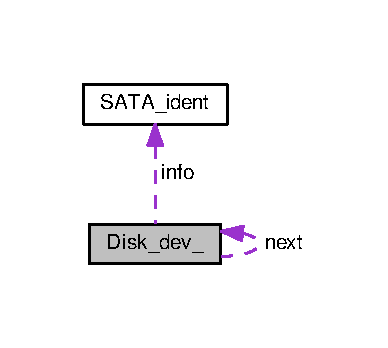
\includegraphics[width=186pt]{structDisk__dev____coll__graph}
\end{center}
\end{figure}
\subsection*{Data Fields}
\begin{DoxyCompactItemize}
\item 
uint32\+\_\+t \hyperlink{structDisk__dev___a89cfdf098591b267dfc55bd79a8e3335}{type}
\item 
\hyperlink{ahci_8h_ace0b5fb17e1a588ab172cbf436c0a3d3}{H\+B\+A\+\_\+\+P\+O\+RT} $\ast$ \hyperlink{structDisk__dev___acdebd9b96abc7fbf3f115417afc7a887}{port}
\item 
\hyperlink{ahci_8h_a5083eb2c708d3697870e3e6e4cc89e53}{S\+A\+T\+A\+\_\+ident\+\_\+t} $\ast$ \hyperlink{structDisk__dev___a52e2a9b907b950dd16310e9580a43424}{info}
\item 
struct \hyperlink{structDisk__dev__}{Disk\+\_\+dev\+\_\+} $\ast$ \hyperlink{structDisk__dev___aac658457b32e23e97c219973d3a65fb5}{next}
\end{DoxyCompactItemize}


\subsection{Detailed Description}


Definition at line 628 of file ahci.\+h.



\subsection{Field Documentation}
\index{Disk\+\_\+dev\+\_\+@{Disk\+\_\+dev\+\_\+}!info@{info}}
\index{info@{info}!Disk\+\_\+dev\+\_\+@{Disk\+\_\+dev\+\_\+}}
\subsubsection[{\texorpdfstring{info}{info}}]{\setlength{\rightskip}{0pt plus 5cm}{\bf S\+A\+T\+A\+\_\+ident\+\_\+t}$\ast$ Disk\+\_\+dev\+\_\+\+::info}\hypertarget{structDisk__dev___a52e2a9b907b950dd16310e9580a43424}{}\label{structDisk__dev___a52e2a9b907b950dd16310e9580a43424}


Definition at line 632 of file ahci.\+h.

\index{Disk\+\_\+dev\+\_\+@{Disk\+\_\+dev\+\_\+}!next@{next}}
\index{next@{next}!Disk\+\_\+dev\+\_\+@{Disk\+\_\+dev\+\_\+}}
\subsubsection[{\texorpdfstring{next}{next}}]{\setlength{\rightskip}{0pt plus 5cm}struct {\bf Disk\+\_\+dev\+\_\+}$\ast$ Disk\+\_\+dev\+\_\+\+::next}\hypertarget{structDisk__dev___aac658457b32e23e97c219973d3a65fb5}{}\label{structDisk__dev___aac658457b32e23e97c219973d3a65fb5}


Definition at line 633 of file ahci.\+h.

\index{Disk\+\_\+dev\+\_\+@{Disk\+\_\+dev\+\_\+}!port@{port}}
\index{port@{port}!Disk\+\_\+dev\+\_\+@{Disk\+\_\+dev\+\_\+}}
\subsubsection[{\texorpdfstring{port}{port}}]{\setlength{\rightskip}{0pt plus 5cm}{\bf H\+B\+A\+\_\+\+P\+O\+RT}$\ast$ Disk\+\_\+dev\+\_\+\+::port}\hypertarget{structDisk__dev___acdebd9b96abc7fbf3f115417afc7a887}{}\label{structDisk__dev___acdebd9b96abc7fbf3f115417afc7a887}


Definition at line 631 of file ahci.\+h.

\index{Disk\+\_\+dev\+\_\+@{Disk\+\_\+dev\+\_\+}!type@{type}}
\index{type@{type}!Disk\+\_\+dev\+\_\+@{Disk\+\_\+dev\+\_\+}}
\subsubsection[{\texorpdfstring{type}{type}}]{\setlength{\rightskip}{0pt plus 5cm}uint32\+\_\+t Disk\+\_\+dev\+\_\+\+::type}\hypertarget{structDisk__dev___a89cfdf098591b267dfc55bd79a8e3335}{}\label{structDisk__dev___a89cfdf098591b267dfc55bd79a8e3335}


Definition at line 630 of file ahci.\+h.



The documentation for this struct was generated from the following file\+:\begin{DoxyCompactItemize}
\item 
Experimental Edition/\+Source/\+Drivers/\+A\+H\+C\+I/\hyperlink{ahci_8h}{ahci.\+h}\end{DoxyCompactItemize}

\hypertarget{structFACP}{}\section{F\+A\+CP Struct Reference}
\label{structFACP}\index{F\+A\+CP@{F\+A\+CP}}
\subsection*{Data Fields}
\begin{DoxyCompactItemize}
\item 
\hyperlink{acpi_8c_a0c8186d9b9b7880309c27230bbb5e69d}{byte} \hyperlink{structFACP_a3ec5cc094770cdaf54942c95b5a4eae3}{Signature} \mbox{[}4\mbox{]}
\item 
\hyperlink{acpi_8c_a74cb93d430006e784da73b8ca406ee6e}{dword} \hyperlink{structFACP_ad27e676e94e75e3d8140a2a8c9fd6bfd}{Length}
\item 
\hyperlink{acpi_8c_a0c8186d9b9b7880309c27230bbb5e69d}{byte} \hyperlink{structFACP_ae5f7c21401a9d170e5c6a3caaa9b74ba}{unneded1} \mbox{[}40-\/8\mbox{]}
\item 
\hyperlink{acpi_8c_a74cb93d430006e784da73b8ca406ee6e}{dword} $\ast$ \hyperlink{structFACP_ae9d89be6ba26f7c9109d901c2daa3a75}{D\+S\+DT}
\item 
\hyperlink{acpi_8c_a0c8186d9b9b7880309c27230bbb5e69d}{byte} \hyperlink{structFACP_a6926f57eda7c9c85a3f7509b1d3080c6}{unneded2} \mbox{[}48-\/44\mbox{]}
\item 
\hyperlink{acpi_8c_a74cb93d430006e784da73b8ca406ee6e}{dword} $\ast$ \hyperlink{structFACP_a1ec5f1557834030b62601ecbf75eae9c}{S\+M\+I\+\_\+\+C\+MD}
\item 
\hyperlink{acpi_8c_a0c8186d9b9b7880309c27230bbb5e69d}{byte} \hyperlink{structFACP_a0ce6f514986cb7577fd80249528d4bf0}{A\+C\+P\+I\+\_\+\+E\+N\+A\+B\+LE}
\item 
\hyperlink{acpi_8c_a0c8186d9b9b7880309c27230bbb5e69d}{byte} \hyperlink{structFACP_ac7a25cb3b147fd2824eee9c6fe06f2e3}{A\+C\+P\+I\+\_\+\+D\+I\+S\+A\+B\+LE}
\item 
\hyperlink{acpi_8c_a0c8186d9b9b7880309c27230bbb5e69d}{byte} \hyperlink{structFACP_aa83604b4fb4ca7634fc6da593f8a9d10}{unneded3} \mbox{[}64-\/54\mbox{]}
\item 
\hyperlink{acpi_8c_a74cb93d430006e784da73b8ca406ee6e}{dword} $\ast$ \hyperlink{structFACP_a60341d35abc5ca9a85e97ec88f2afa0c}{P\+M1a\+\_\+\+C\+N\+T\+\_\+\+B\+LK}
\item 
\hyperlink{acpi_8c_a74cb93d430006e784da73b8ca406ee6e}{dword} $\ast$ \hyperlink{structFACP_a3f6c4a12d7aaa5b666230cb71d694e5b}{P\+M1b\+\_\+\+C\+N\+T\+\_\+\+B\+LK}
\item 
\hyperlink{acpi_8c_a0c8186d9b9b7880309c27230bbb5e69d}{byte} \hyperlink{structFACP_a8309a4015441febd7eebf3ed7524c2e7}{unneded4} \mbox{[}89-\/72\mbox{]}
\item 
\hyperlink{acpi_8c_a0c8186d9b9b7880309c27230bbb5e69d}{byte} \hyperlink{structFACP_aef6c96d35d4c773fb1e06e9baacd2a5f}{P\+M1\+\_\+\+C\+N\+T\+\_\+\+L\+EN}
\end{DoxyCompactItemize}


\subsection{Detailed Description}


Definition at line 36 of file acpi.\+c.



\subsection{Field Documentation}
\index{F\+A\+CP@{F\+A\+CP}!A\+C\+P\+I\+\_\+\+D\+I\+S\+A\+B\+LE@{A\+C\+P\+I\+\_\+\+D\+I\+S\+A\+B\+LE}}
\index{A\+C\+P\+I\+\_\+\+D\+I\+S\+A\+B\+LE@{A\+C\+P\+I\+\_\+\+D\+I\+S\+A\+B\+LE}!F\+A\+CP@{F\+A\+CP}}
\subsubsection[{\texorpdfstring{A\+C\+P\+I\+\_\+\+D\+I\+S\+A\+B\+LE}{ACPI_DISABLE}}]{\setlength{\rightskip}{0pt plus 5cm}{\bf byte} F\+A\+C\+P\+::\+A\+C\+P\+I\+\_\+\+D\+I\+S\+A\+B\+LE}\hypertarget{structFACP_ac7a25cb3b147fd2824eee9c6fe06f2e3}{}\label{structFACP_ac7a25cb3b147fd2824eee9c6fe06f2e3}


Definition at line 45 of file acpi.\+c.

\index{F\+A\+CP@{F\+A\+CP}!A\+C\+P\+I\+\_\+\+E\+N\+A\+B\+LE@{A\+C\+P\+I\+\_\+\+E\+N\+A\+B\+LE}}
\index{A\+C\+P\+I\+\_\+\+E\+N\+A\+B\+LE@{A\+C\+P\+I\+\_\+\+E\+N\+A\+B\+LE}!F\+A\+CP@{F\+A\+CP}}
\subsubsection[{\texorpdfstring{A\+C\+P\+I\+\_\+\+E\+N\+A\+B\+LE}{ACPI_ENABLE}}]{\setlength{\rightskip}{0pt plus 5cm}{\bf byte} F\+A\+C\+P\+::\+A\+C\+P\+I\+\_\+\+E\+N\+A\+B\+LE}\hypertarget{structFACP_a0ce6f514986cb7577fd80249528d4bf0}{}\label{structFACP_a0ce6f514986cb7577fd80249528d4bf0}


Definition at line 44 of file acpi.\+c.

\index{F\+A\+CP@{F\+A\+CP}!D\+S\+DT@{D\+S\+DT}}
\index{D\+S\+DT@{D\+S\+DT}!F\+A\+CP@{F\+A\+CP}}
\subsubsection[{\texorpdfstring{D\+S\+DT}{DSDT}}]{\setlength{\rightskip}{0pt plus 5cm}{\bf dword}$\ast$ F\+A\+C\+P\+::\+D\+S\+DT}\hypertarget{structFACP_ae9d89be6ba26f7c9109d901c2daa3a75}{}\label{structFACP_ae9d89be6ba26f7c9109d901c2daa3a75}


Definition at line 41 of file acpi.\+c.

\index{F\+A\+CP@{F\+A\+CP}!Length@{Length}}
\index{Length@{Length}!F\+A\+CP@{F\+A\+CP}}
\subsubsection[{\texorpdfstring{Length}{Length}}]{\setlength{\rightskip}{0pt plus 5cm}{\bf dword} F\+A\+C\+P\+::\+Length}\hypertarget{structFACP_ad27e676e94e75e3d8140a2a8c9fd6bfd}{}\label{structFACP_ad27e676e94e75e3d8140a2a8c9fd6bfd}


Definition at line 39 of file acpi.\+c.

\index{F\+A\+CP@{F\+A\+CP}!P\+M1\+\_\+\+C\+N\+T\+\_\+\+L\+EN@{P\+M1\+\_\+\+C\+N\+T\+\_\+\+L\+EN}}
\index{P\+M1\+\_\+\+C\+N\+T\+\_\+\+L\+EN@{P\+M1\+\_\+\+C\+N\+T\+\_\+\+L\+EN}!F\+A\+CP@{F\+A\+CP}}
\subsubsection[{\texorpdfstring{P\+M1\+\_\+\+C\+N\+T\+\_\+\+L\+EN}{PM1_CNT_LEN}}]{\setlength{\rightskip}{0pt plus 5cm}{\bf byte} F\+A\+C\+P\+::\+P\+M1\+\_\+\+C\+N\+T\+\_\+\+L\+EN}\hypertarget{structFACP_aef6c96d35d4c773fb1e06e9baacd2a5f}{}\label{structFACP_aef6c96d35d4c773fb1e06e9baacd2a5f}


Definition at line 50 of file acpi.\+c.

\index{F\+A\+CP@{F\+A\+CP}!P\+M1a\+\_\+\+C\+N\+T\+\_\+\+B\+LK@{P\+M1a\+\_\+\+C\+N\+T\+\_\+\+B\+LK}}
\index{P\+M1a\+\_\+\+C\+N\+T\+\_\+\+B\+LK@{P\+M1a\+\_\+\+C\+N\+T\+\_\+\+B\+LK}!F\+A\+CP@{F\+A\+CP}}
\subsubsection[{\texorpdfstring{P\+M1a\+\_\+\+C\+N\+T\+\_\+\+B\+LK}{PM1a_CNT_BLK}}]{\setlength{\rightskip}{0pt plus 5cm}{\bf dword}$\ast$ F\+A\+C\+P\+::\+P\+M1a\+\_\+\+C\+N\+T\+\_\+\+B\+LK}\hypertarget{structFACP_a60341d35abc5ca9a85e97ec88f2afa0c}{}\label{structFACP_a60341d35abc5ca9a85e97ec88f2afa0c}


Definition at line 47 of file acpi.\+c.

\index{F\+A\+CP@{F\+A\+CP}!P\+M1b\+\_\+\+C\+N\+T\+\_\+\+B\+LK@{P\+M1b\+\_\+\+C\+N\+T\+\_\+\+B\+LK}}
\index{P\+M1b\+\_\+\+C\+N\+T\+\_\+\+B\+LK@{P\+M1b\+\_\+\+C\+N\+T\+\_\+\+B\+LK}!F\+A\+CP@{F\+A\+CP}}
\subsubsection[{\texorpdfstring{P\+M1b\+\_\+\+C\+N\+T\+\_\+\+B\+LK}{PM1b_CNT_BLK}}]{\setlength{\rightskip}{0pt plus 5cm}{\bf dword}$\ast$ F\+A\+C\+P\+::\+P\+M1b\+\_\+\+C\+N\+T\+\_\+\+B\+LK}\hypertarget{structFACP_a3f6c4a12d7aaa5b666230cb71d694e5b}{}\label{structFACP_a3f6c4a12d7aaa5b666230cb71d694e5b}


Definition at line 48 of file acpi.\+c.

\index{F\+A\+CP@{F\+A\+CP}!Signature@{Signature}}
\index{Signature@{Signature}!F\+A\+CP@{F\+A\+CP}}
\subsubsection[{\texorpdfstring{Signature}{Signature}}]{\setlength{\rightskip}{0pt plus 5cm}{\bf byte} F\+A\+C\+P\+::\+Signature\mbox{[}4\mbox{]}}\hypertarget{structFACP_a3ec5cc094770cdaf54942c95b5a4eae3}{}\label{structFACP_a3ec5cc094770cdaf54942c95b5a4eae3}


Definition at line 38 of file acpi.\+c.

\index{F\+A\+CP@{F\+A\+CP}!S\+M\+I\+\_\+\+C\+MD@{S\+M\+I\+\_\+\+C\+MD}}
\index{S\+M\+I\+\_\+\+C\+MD@{S\+M\+I\+\_\+\+C\+MD}!F\+A\+CP@{F\+A\+CP}}
\subsubsection[{\texorpdfstring{S\+M\+I\+\_\+\+C\+MD}{SMI_CMD}}]{\setlength{\rightskip}{0pt plus 5cm}{\bf dword}$\ast$ F\+A\+C\+P\+::\+S\+M\+I\+\_\+\+C\+MD}\hypertarget{structFACP_a1ec5f1557834030b62601ecbf75eae9c}{}\label{structFACP_a1ec5f1557834030b62601ecbf75eae9c}


Definition at line 43 of file acpi.\+c.

\index{F\+A\+CP@{F\+A\+CP}!unneded1@{unneded1}}
\index{unneded1@{unneded1}!F\+A\+CP@{F\+A\+CP}}
\subsubsection[{\texorpdfstring{unneded1}{unneded1}}]{\setlength{\rightskip}{0pt plus 5cm}{\bf byte} F\+A\+C\+P\+::unneded1\mbox{[}40-\/8\mbox{]}}\hypertarget{structFACP_ae5f7c21401a9d170e5c6a3caaa9b74ba}{}\label{structFACP_ae5f7c21401a9d170e5c6a3caaa9b74ba}


Definition at line 40 of file acpi.\+c.

\index{F\+A\+CP@{F\+A\+CP}!unneded2@{unneded2}}
\index{unneded2@{unneded2}!F\+A\+CP@{F\+A\+CP}}
\subsubsection[{\texorpdfstring{unneded2}{unneded2}}]{\setlength{\rightskip}{0pt plus 5cm}{\bf byte} F\+A\+C\+P\+::unneded2\mbox{[}48-\/44\mbox{]}}\hypertarget{structFACP_a6926f57eda7c9c85a3f7509b1d3080c6}{}\label{structFACP_a6926f57eda7c9c85a3f7509b1d3080c6}


Definition at line 42 of file acpi.\+c.

\index{F\+A\+CP@{F\+A\+CP}!unneded3@{unneded3}}
\index{unneded3@{unneded3}!F\+A\+CP@{F\+A\+CP}}
\subsubsection[{\texorpdfstring{unneded3}{unneded3}}]{\setlength{\rightskip}{0pt plus 5cm}{\bf byte} F\+A\+C\+P\+::unneded3\mbox{[}64-\/54\mbox{]}}\hypertarget{structFACP_aa83604b4fb4ca7634fc6da593f8a9d10}{}\label{structFACP_aa83604b4fb4ca7634fc6da593f8a9d10}


Definition at line 46 of file acpi.\+c.

\index{F\+A\+CP@{F\+A\+CP}!unneded4@{unneded4}}
\index{unneded4@{unneded4}!F\+A\+CP@{F\+A\+CP}}
\subsubsection[{\texorpdfstring{unneded4}{unneded4}}]{\setlength{\rightskip}{0pt plus 5cm}{\bf byte} F\+A\+C\+P\+::unneded4\mbox{[}89-\/72\mbox{]}}\hypertarget{structFACP_a8309a4015441febd7eebf3ed7524c2e7}{}\label{structFACP_a8309a4015441febd7eebf3ed7524c2e7}


Definition at line 49 of file acpi.\+c.



The documentation for this struct was generated from the following file\+:\begin{DoxyCompactItemize}
\item 
Experimental Edition/\+Source/\+Drivers/\+A\+C\+P\+I/\hyperlink{acpi_8c}{acpi.\+c}\end{DoxyCompactItemize}

\hypertarget{structfile}{}\section{file Struct Reference}
\label{structfile}\index{file@{file}}


{\ttfamily \#include $<$common.\+h$>$}

\subsection*{Data Fields}
\begin{DoxyCompactItemize}
\item 
int \hyperlink{structfile_a3786bd6e6b62b6a56d906c4ab40f0648}{inode\+\_\+num}
\item 
char \hyperlink{structfile_ad45e3551765b38ecf4598ee9b06c796f}{filename} \mbox{[}100\mbox{]}
\item 
int \hyperlink{structfile_ad094e8384225dee8ae9b4258745c30f9}{perm}
\item 
int \hyperlink{structfile_a83a90719edeee627bd6fefe5f8af58ce}{size}
\item 
char \hyperlink{structfile_a814f6220d71e264dc20aaaec301d99e7}{type}
\item 
int \hyperlink{structfile_ab4368e129b54f18c028265ad49779e04}{sector\+\_\+loc} \mbox{[}10\mbox{]}
\item 
int \hyperlink{structfile_ad056d2081f3cab9ed4668689a02acaaf}{offset}
\item 
uint64\+\_\+t \hyperlink{structfile_afc95f13cca3cd7a46d733717a5f4a6ed}{address}
\item 
int \hyperlink{structfile_a3161116c6ac521cfa3514f02c88b8d65}{is\+\_\+fs}
\end{DoxyCompactItemize}


\subsection{Detailed Description}


Definition at line 55 of file common.\+h.



\subsection{Field Documentation}
\index{file@{file}!address@{address}}
\index{address@{address}!file@{file}}
\subsubsection[{\texorpdfstring{address}{address}}]{\setlength{\rightskip}{0pt plus 5cm}uint64\+\_\+t file\+::address}\hypertarget{structfile_afc95f13cca3cd7a46d733717a5f4a6ed}{}\label{structfile_afc95f13cca3cd7a46d733717a5f4a6ed}


Definition at line 63 of file common.\+h.

\index{file@{file}!filename@{filename}}
\index{filename@{filename}!file@{file}}
\subsubsection[{\texorpdfstring{filename}{filename}}]{\setlength{\rightskip}{0pt plus 5cm}char file\+::filename\mbox{[}100\mbox{]}}\hypertarget{structfile_ad45e3551765b38ecf4598ee9b06c796f}{}\label{structfile_ad45e3551765b38ecf4598ee9b06c796f}


Definition at line 57 of file common.\+h.

\index{file@{file}!inode\+\_\+num@{inode\+\_\+num}}
\index{inode\+\_\+num@{inode\+\_\+num}!file@{file}}
\subsubsection[{\texorpdfstring{inode\+\_\+num}{inode_num}}]{\setlength{\rightskip}{0pt plus 5cm}int file\+::inode\+\_\+num}\hypertarget{structfile_a3786bd6e6b62b6a56d906c4ab40f0648}{}\label{structfile_a3786bd6e6b62b6a56d906c4ab40f0648}


Definition at line 56 of file common.\+h.

\index{file@{file}!is\+\_\+fs@{is\+\_\+fs}}
\index{is\+\_\+fs@{is\+\_\+fs}!file@{file}}
\subsubsection[{\texorpdfstring{is\+\_\+fs}{is_fs}}]{\setlength{\rightskip}{0pt plus 5cm}int file\+::is\+\_\+fs}\hypertarget{structfile_a3161116c6ac521cfa3514f02c88b8d65}{}\label{structfile_a3161116c6ac521cfa3514f02c88b8d65}


Definition at line 64 of file common.\+h.

\index{file@{file}!offset@{offset}}
\index{offset@{offset}!file@{file}}
\subsubsection[{\texorpdfstring{offset}{offset}}]{\setlength{\rightskip}{0pt plus 5cm}int file\+::offset}\hypertarget{structfile_ad056d2081f3cab9ed4668689a02acaaf}{}\label{structfile_ad056d2081f3cab9ed4668689a02acaaf}


Definition at line 62 of file common.\+h.

\index{file@{file}!perm@{perm}}
\index{perm@{perm}!file@{file}}
\subsubsection[{\texorpdfstring{perm}{perm}}]{\setlength{\rightskip}{0pt plus 5cm}int file\+::perm}\hypertarget{structfile_ad094e8384225dee8ae9b4258745c30f9}{}\label{structfile_ad094e8384225dee8ae9b4258745c30f9}


Definition at line 58 of file common.\+h.

\index{file@{file}!sector\+\_\+loc@{sector\+\_\+loc}}
\index{sector\+\_\+loc@{sector\+\_\+loc}!file@{file}}
\subsubsection[{\texorpdfstring{sector\+\_\+loc}{sector_loc}}]{\setlength{\rightskip}{0pt plus 5cm}int file\+::sector\+\_\+loc\mbox{[}10\mbox{]}}\hypertarget{structfile_ab4368e129b54f18c028265ad49779e04}{}\label{structfile_ab4368e129b54f18c028265ad49779e04}


Definition at line 61 of file common.\+h.

\index{file@{file}!size@{size}}
\index{size@{size}!file@{file}}
\subsubsection[{\texorpdfstring{size}{size}}]{\setlength{\rightskip}{0pt plus 5cm}int file\+::size}\hypertarget{structfile_a83a90719edeee627bd6fefe5f8af58ce}{}\label{structfile_a83a90719edeee627bd6fefe5f8af58ce}


Definition at line 59 of file common.\+h.

\index{file@{file}!type@{type}}
\index{type@{type}!file@{file}}
\subsubsection[{\texorpdfstring{type}{type}}]{\setlength{\rightskip}{0pt plus 5cm}char file\+::type}\hypertarget{structfile_a814f6220d71e264dc20aaaec301d99e7}{}\label{structfile_a814f6220d71e264dc20aaaec301d99e7}


Definition at line 60 of file common.\+h.



The documentation for this struct was generated from the following file\+:\begin{DoxyCompactItemize}
\item 
Experimental Edition/\+Library/\hyperlink{common_8h}{common.\+h}\end{DoxyCompactItemize}

\hypertarget{structgdt__entry__struct}{}\section{gdt\+\_\+entry\+\_\+struct Struct Reference}
\label{structgdt__entry__struct}\index{gdt\+\_\+entry\+\_\+struct@{gdt\+\_\+entry\+\_\+struct}}


{\ttfamily \#include $<$descriptors.\+h$>$}

\subsection*{Data Fields}
\begin{DoxyCompactItemize}
\item 
uint16\+\_\+t \hyperlink{structgdt__entry__struct_a6bbf5ad7af7b8e8e7f7c26ec74d8c1b2}{limit\+\_\+low}
\item 
uint16\+\_\+t \hyperlink{structgdt__entry__struct_adba88eafea5f07167d181e4090cbcf49}{base\+\_\+low}
\item 
uint8\+\_\+t \hyperlink{structgdt__entry__struct_a986d46963d3ccdbec85b3749c1e09abf}{base\+\_\+middle}
\item 
uint8\+\_\+t \hyperlink{structgdt__entry__struct_ac07173385496c5b952e58ddc20f1cc99}{access}
\item 
uint8\+\_\+t \hyperlink{structgdt__entry__struct_a7fb7b3704e10434dbe64564416cf1a25}{granularity}
\item 
uint8\+\_\+t \hyperlink{structgdt__entry__struct_aa08eedea9c0f707b9fa052b7567879c7}{base\+\_\+high}
\end{DoxyCompactItemize}


\subsection{Detailed Description}


Definition at line 3 of file descriptors.\+h.



\subsection{Field Documentation}
\index{gdt\+\_\+entry\+\_\+struct@{gdt\+\_\+entry\+\_\+struct}!access@{access}}
\index{access@{access}!gdt\+\_\+entry\+\_\+struct@{gdt\+\_\+entry\+\_\+struct}}
\subsubsection[{\texorpdfstring{access}{access}}]{\setlength{\rightskip}{0pt plus 5cm}uint8\+\_\+t gdt\+\_\+entry\+\_\+struct\+::access}\hypertarget{structgdt__entry__struct_ac07173385496c5b952e58ddc20f1cc99}{}\label{structgdt__entry__struct_ac07173385496c5b952e58ddc20f1cc99}


Definition at line 8 of file descriptors.\+h.

\index{gdt\+\_\+entry\+\_\+struct@{gdt\+\_\+entry\+\_\+struct}!base\+\_\+high@{base\+\_\+high}}
\index{base\+\_\+high@{base\+\_\+high}!gdt\+\_\+entry\+\_\+struct@{gdt\+\_\+entry\+\_\+struct}}
\subsubsection[{\texorpdfstring{base\+\_\+high}{base_high}}]{\setlength{\rightskip}{0pt plus 5cm}uint8\+\_\+t gdt\+\_\+entry\+\_\+struct\+::base\+\_\+high}\hypertarget{structgdt__entry__struct_aa08eedea9c0f707b9fa052b7567879c7}{}\label{structgdt__entry__struct_aa08eedea9c0f707b9fa052b7567879c7}


Definition at line 10 of file descriptors.\+h.

\index{gdt\+\_\+entry\+\_\+struct@{gdt\+\_\+entry\+\_\+struct}!base\+\_\+low@{base\+\_\+low}}
\index{base\+\_\+low@{base\+\_\+low}!gdt\+\_\+entry\+\_\+struct@{gdt\+\_\+entry\+\_\+struct}}
\subsubsection[{\texorpdfstring{base\+\_\+low}{base_low}}]{\setlength{\rightskip}{0pt plus 5cm}uint16\+\_\+t gdt\+\_\+entry\+\_\+struct\+::base\+\_\+low}\hypertarget{structgdt__entry__struct_adba88eafea5f07167d181e4090cbcf49}{}\label{structgdt__entry__struct_adba88eafea5f07167d181e4090cbcf49}


Definition at line 6 of file descriptors.\+h.

\index{gdt\+\_\+entry\+\_\+struct@{gdt\+\_\+entry\+\_\+struct}!base\+\_\+middle@{base\+\_\+middle}}
\index{base\+\_\+middle@{base\+\_\+middle}!gdt\+\_\+entry\+\_\+struct@{gdt\+\_\+entry\+\_\+struct}}
\subsubsection[{\texorpdfstring{base\+\_\+middle}{base_middle}}]{\setlength{\rightskip}{0pt plus 5cm}uint8\+\_\+t gdt\+\_\+entry\+\_\+struct\+::base\+\_\+middle}\hypertarget{structgdt__entry__struct_a986d46963d3ccdbec85b3749c1e09abf}{}\label{structgdt__entry__struct_a986d46963d3ccdbec85b3749c1e09abf}


Definition at line 7 of file descriptors.\+h.

\index{gdt\+\_\+entry\+\_\+struct@{gdt\+\_\+entry\+\_\+struct}!granularity@{granularity}}
\index{granularity@{granularity}!gdt\+\_\+entry\+\_\+struct@{gdt\+\_\+entry\+\_\+struct}}
\subsubsection[{\texorpdfstring{granularity}{granularity}}]{\setlength{\rightskip}{0pt plus 5cm}uint8\+\_\+t gdt\+\_\+entry\+\_\+struct\+::granularity}\hypertarget{structgdt__entry__struct_a7fb7b3704e10434dbe64564416cf1a25}{}\label{structgdt__entry__struct_a7fb7b3704e10434dbe64564416cf1a25}


Definition at line 9 of file descriptors.\+h.

\index{gdt\+\_\+entry\+\_\+struct@{gdt\+\_\+entry\+\_\+struct}!limit\+\_\+low@{limit\+\_\+low}}
\index{limit\+\_\+low@{limit\+\_\+low}!gdt\+\_\+entry\+\_\+struct@{gdt\+\_\+entry\+\_\+struct}}
\subsubsection[{\texorpdfstring{limit\+\_\+low}{limit_low}}]{\setlength{\rightskip}{0pt plus 5cm}uint16\+\_\+t gdt\+\_\+entry\+\_\+struct\+::limit\+\_\+low}\hypertarget{structgdt__entry__struct_a6bbf5ad7af7b8e8e7f7c26ec74d8c1b2}{}\label{structgdt__entry__struct_a6bbf5ad7af7b8e8e7f7c26ec74d8c1b2}


Definition at line 5 of file descriptors.\+h.



The documentation for this struct was generated from the following file\+:\begin{DoxyCompactItemize}
\item 
Experimental Edition/\+Source/\+G\+D\+T\+\_\+\+I\+D\+T/\hyperlink{descriptors_8h}{descriptors.\+h}\end{DoxyCompactItemize}

\hypertarget{structgdt__ptr__struct}{}\section{gdt\+\_\+ptr\+\_\+struct Struct Reference}
\label{structgdt__ptr__struct}\index{gdt\+\_\+ptr\+\_\+struct@{gdt\+\_\+ptr\+\_\+struct}}


{\ttfamily \#include $<$descriptors.\+h$>$}

\subsection*{Data Fields}
\begin{DoxyCompactItemize}
\item 
uint16\+\_\+t \hyperlink{structgdt__ptr__struct_abf557ff0ca1cf3e130e8ab0086ab4ce6}{limit}
\item 
uint32\+\_\+t \hyperlink{structgdt__ptr__struct_a9b351f31bc261f3c2c3a87252350fb9c}{base}
\end{DoxyCompactItemize}


\subsection{Detailed Description}


Definition at line 14 of file descriptors.\+h.



\subsection{Field Documentation}
\index{gdt\+\_\+ptr\+\_\+struct@{gdt\+\_\+ptr\+\_\+struct}!base@{base}}
\index{base@{base}!gdt\+\_\+ptr\+\_\+struct@{gdt\+\_\+ptr\+\_\+struct}}
\subsubsection[{\texorpdfstring{base}{base}}]{\setlength{\rightskip}{0pt plus 5cm}uint32\+\_\+t gdt\+\_\+ptr\+\_\+struct\+::base}\hypertarget{structgdt__ptr__struct_a9b351f31bc261f3c2c3a87252350fb9c}{}\label{structgdt__ptr__struct_a9b351f31bc261f3c2c3a87252350fb9c}


Definition at line 17 of file descriptors.\+h.

\index{gdt\+\_\+ptr\+\_\+struct@{gdt\+\_\+ptr\+\_\+struct}!limit@{limit}}
\index{limit@{limit}!gdt\+\_\+ptr\+\_\+struct@{gdt\+\_\+ptr\+\_\+struct}}
\subsubsection[{\texorpdfstring{limit}{limit}}]{\setlength{\rightskip}{0pt plus 5cm}uint16\+\_\+t gdt\+\_\+ptr\+\_\+struct\+::limit}\hypertarget{structgdt__ptr__struct_abf557ff0ca1cf3e130e8ab0086ab4ce6}{}\label{structgdt__ptr__struct_abf557ff0ca1cf3e130e8ab0086ab4ce6}


Definition at line 16 of file descriptors.\+h.



The documentation for this struct was generated from the following file\+:\begin{DoxyCompactItemize}
\item 
Experimental Edition/\+Source/\+G\+D\+T\+\_\+\+I\+D\+T/\hyperlink{descriptors_8h}{descriptors.\+h}\end{DoxyCompactItemize}

\hypertarget{structident__device__t}{}\section{ident\+\_\+device\+\_\+t Struct Reference}
\label{structident__device__t}\index{ident\+\_\+device\+\_\+t@{ident\+\_\+device\+\_\+t}}


{\ttfamily \#include $<$ata.\+h$>$}

\subsection*{Data Fields}
\begin{DoxyCompactItemize}
\item 
unsigned short \hyperlink{structident__device__t_a244665cc61b5b3e5fcec35242a01fc9b}{config}
\item 
unsigned short \hyperlink{structident__device__t_a99303affca63361d7b97f40fd29b1028}{cyls}
\item 
unsigned short \hyperlink{structident__device__t_ab16b1b188cf48d9f8e7b510e3eb9933c}{reserved2}
\item 
unsigned short \hyperlink{structident__device__t_abe75fc82f62aeb25eeeaebc14832cee5}{heads}
\item 
unsigned short \hyperlink{structident__device__t_ac5bfb23af07632fcb7ab55872b7e8839}{track\+\_\+bytes}
\item 
unsigned short \hyperlink{structident__device__t_a65aac348597065dd666c8d17d5436cfe}{sector\+\_\+bytes}
\item 
unsigned short \hyperlink{structident__device__t_a0936bf38dc570c2117003696aef259ab}{sectors}
\item 
unsigned short \hyperlink{structident__device__t_ad4057b661fe03727c4c8c5c131beba91}{vendor0}
\item 
unsigned short \hyperlink{structident__device__t_a690a82fc5e0d922b28a2706e57298ef0}{vendor1}
\item 
unsigned short \hyperlink{structident__device__t_a9d34132aa72f1591baa59ce870e626e1}{vendor2}
\item 
unsigned char \hyperlink{structident__device__t_aa2f154afca4db0b73806e565ecf79bfb}{serial\+\_\+no} \mbox{[}20\mbox{]}
\item 
unsigned short \hyperlink{structident__device__t_aa631ed68393ce9dcc8dfac663441a14d}{buf\+\_\+type}
\item 
unsigned short \hyperlink{structident__device__t_a2b96de1287d6347279fb208225262974}{buf\+\_\+size}
\item 
unsigned short \hyperlink{structident__device__t_af5aba8d177b13759ad10593aefef75de}{ecc\+\_\+bytes}
\item 
unsigned char \hyperlink{structident__device__t_a17cf9b96ebf881a367f7c4807d9e4ebc}{fw\+\_\+rev} \mbox{[}8\mbox{]}
\item 
unsigned char \hyperlink{structident__device__t_a04219740c47641a652b946bd7bbcdaf6}{model} \mbox{[}40\mbox{]}
\item 
unsigned char \hyperlink{structident__device__t_a8238d2f55c2d2f68ccdf0e20029fe636}{max\+\_\+multsect}
\item 
unsigned char \hyperlink{structident__device__t_a3812ae5e744328c081f25c0f4ecaec63}{vendor3}
\item 
unsigned short \hyperlink{structident__device__t_a8105ba5d1d0794158b141ddba3b396c4}{dword\+\_\+io}
\item 
unsigned char \hyperlink{structident__device__t_a1484d43f0a155e4fb3efa6d00eadc0d1}{vendor4}
\item 
unsigned char \hyperlink{structident__device__t_a7d02a0251de92f8bfcde9254fae00d51}{capability}
\item 
unsigned short \hyperlink{structident__device__t_ae77410f26a7ef148d5d17fb5a068f135}{reserved50}
\item 
unsigned char \hyperlink{structident__device__t_aa37d90e0a3dbaf28b2b20ee7a792ca37}{vendor5}
\item 
unsigned char \hyperlink{structident__device__t_a98aef15c0899c883fad89b60d712d4cb}{t\+P\+IO}
\item 
unsigned char \hyperlink{structident__device__t_a51b7a29370473491cdad8e6fbafce21a}{vendor6}
\item 
unsigned char \hyperlink{structident__device__t_a06c2602918273e7e0b9163eeb9fa68e3}{t\+D\+MA}
\item 
unsigned short \hyperlink{structident__device__t_ae127ec2092115637970e5993909d6c02}{field\+\_\+valid}
\item 
unsigned short \hyperlink{structident__device__t_a5d2e9e636ff4e9fa7b73d52411c94e9c}{cur\+\_\+cyls}
\item 
unsigned short \hyperlink{structident__device__t_a35e272894045c082fa9b34630b270d2c}{cur\+\_\+heads}
\item 
unsigned short \hyperlink{structident__device__t_ae4e4455f7d44a28f3d2d914739ba73ed}{cur\+\_\+sectors}
\item 
unsigned short \hyperlink{structident__device__t_a15f93e46e5a465a66e1116bb4ebacd44}{cur\+\_\+capacity0}
\item 
unsigned short \hyperlink{structident__device__t_ae60fada7975afcb92375bd112a7103ad}{cur\+\_\+capacity1}
\item 
unsigned char \hyperlink{structident__device__t_a3be5a1bc892f8c1a4565d2a5a604a19e}{multsect}
\item 
unsigned char \hyperlink{structident__device__t_a6749281572514b27f7e71126f9f8df1c}{multsect\+\_\+valid}
\item 
unsigned int \hyperlink{structident__device__t_a81cce22064b24fead62dc0b8b1a8ea3d}{lba\+\_\+capacity}
\item 
unsigned short \hyperlink{structident__device__t_a478243c429923306e486400604e8bdee}{dma\+\_\+1word}
\item 
unsigned short \hyperlink{structident__device__t_a125ef700c585b4f13f3ed51f9808ec19}{dma\+\_\+mword}
\item 
unsigned short \hyperlink{structident__device__t_aa47dec5c44da729522f14edc7ca02f8b}{eide\+\_\+pio\+\_\+modes}
\item 
unsigned short \hyperlink{structident__device__t_ac9b15de363f7fe0dcc8ca3c1a5bc9989}{eide\+\_\+dma\+\_\+min}
\item 
unsigned short \hyperlink{structident__device__t_a3f67d5fd310f8f431fe807350616878f}{eide\+\_\+dma\+\_\+time}
\item 
unsigned short \hyperlink{structident__device__t_a6dc57a8c2a8ba3ce73ad1d48a8c22178}{eide\+\_\+pio}
\item 
unsigned short \hyperlink{structident__device__t_a5dda74b9cc6f4458e81f91cb2b1d6a1d}{eide\+\_\+pio\+\_\+iordy}
\item 
unsigned short \hyperlink{structident__device__t_a18de334971e876ab5fb98bbeee82805a}{words69\+\_\+70} \mbox{[}2\mbox{]}
\item 
unsigned short \hyperlink{structident__device__t_ae94ab7c98a95dea40ac23a93b24be1fa}{words71\+\_\+74} \mbox{[}4\mbox{]}
\item 
unsigned short \hyperlink{structident__device__t_ac1f7e4bfd3701c7823bec39bafa1292b}{queue\+\_\+depth}
\item 
unsigned short \hyperlink{structident__device__t_a49b7f672d60d273ea4c6b12b45677bab}{words76\+\_\+79} \mbox{[}4\mbox{]}
\item 
unsigned short \hyperlink{structident__device__t_abece23d6f89f4a6baa5f961b9c265e8c}{major\+\_\+rev\+\_\+num}
\item 
unsigned short \hyperlink{structident__device__t_a32613085d76e1845af675c4559dd4288}{minor\+\_\+rev\+\_\+num}
\item 
unsigned short \hyperlink{structident__device__t_a4eb0292566454e00ecba5e5a0d8e613f}{command\+\_\+set\+\_\+1}
\item 
unsigned short \hyperlink{structident__device__t_abd3639653bdac02a650a0c263e2d6dc3}{command\+\_\+set\+\_\+2}
\item 
unsigned short \hyperlink{structident__device__t_a471a93b5ad51421739da90fb7411098c}{cfsse}
\item 
unsigned short \hyperlink{structident__device__t_a0ec1d5bb87dd9448de785f41e9c227bb}{cfs\+\_\+enable\+\_\+1}
\item 
unsigned short \hyperlink{structident__device__t_a9c56b377c273470a41e0c13b9681fe9e}{cfs\+\_\+enable\+\_\+2}
\item 
unsigned short \hyperlink{structident__device__t_a47ec6f0b2fe379bdd5af96c966c3cf26}{csf\+\_\+default}
\item 
unsigned short \hyperlink{structident__device__t_a380b2b09664f4058c69ab22e54e71c59}{dma\+\_\+ultra}
\item 
unsigned short \hyperlink{structident__device__t_afe35780760139a739638cfe4e3b93fb9}{word89}
\item 
unsigned short \hyperlink{structident__device__t_aecb00df2d3c8414264a12b6ddb8afcb8}{word90}
\item 
unsigned short \hyperlink{structident__device__t_a7e34107276efe12de800e1dba6b9e476}{Cur\+A\+P\+Mvalues}
\item 
unsigned short \hyperlink{structident__device__t_a8ec1dbaa797ef886e2c7ba8b4940f442}{word92}
\item 
unsigned short \hyperlink{structident__device__t_a1f9499790ad26349d6df3e7c8f52c2fa}{hw\+\_\+config}
\item 
unsigned short \hyperlink{structident__device__t_a32485bac63213d7c0780a89df8b066e3}{words94\+\_\+125} \mbox{[}32\mbox{]}
\item 
unsigned short \hyperlink{structident__device__t_a58554aa90ee1104efe6839cd224570a0}{last\+\_\+lun}
\item 
unsigned short \hyperlink{structident__device__t_aafda7436375102d5165194c20b9c4861}{word127}
\item 
unsigned short \hyperlink{structident__device__t_a4dbb8da5f32a2d02cee8365d22ce3b68}{dlf}
\item 
unsigned short \hyperlink{structident__device__t_aadfa929967cf77a8dd7338516b3b39b4}{csfo}
\item 
unsigned short \hyperlink{structident__device__t_a663ba0f8b9d12f16691962d97e269d22}{words130\+\_\+155} \mbox{[}26\mbox{]}
\item 
unsigned short \hyperlink{structident__device__t_ab2883d4ef22029232a95fc6c7fc1489b}{word156}
\item 
unsigned short \hyperlink{structident__device__t_a3be0642d7da6a8ba1cc4e4efe30e4058}{words157\+\_\+159} \mbox{[}3\mbox{]}
\item 
unsigned short \hyperlink{structident__device__t_a9a4568ee4fc1d39076c9338ab8aa1970}{words160\+\_\+255} \mbox{[}95\mbox{]}
\end{DoxyCompactItemize}


\subsection{Detailed Description}


Definition at line 163 of file ata.\+h.



\subsection{Field Documentation}
\index{ident\+\_\+device\+\_\+t@{ident\+\_\+device\+\_\+t}!buf\+\_\+size@{buf\+\_\+size}}
\index{buf\+\_\+size@{buf\+\_\+size}!ident\+\_\+device\+\_\+t@{ident\+\_\+device\+\_\+t}}
\subsubsection[{\texorpdfstring{buf\+\_\+size}{buf_size}}]{\setlength{\rightskip}{0pt plus 5cm}unsigned short ident\+\_\+device\+\_\+t\+::buf\+\_\+size}\hypertarget{structident__device__t_a2b96de1287d6347279fb208225262974}{}\label{structident__device__t_a2b96de1287d6347279fb208225262974}


Definition at line 176 of file ata.\+h.

\index{ident\+\_\+device\+\_\+t@{ident\+\_\+device\+\_\+t}!buf\+\_\+type@{buf\+\_\+type}}
\index{buf\+\_\+type@{buf\+\_\+type}!ident\+\_\+device\+\_\+t@{ident\+\_\+device\+\_\+t}}
\subsubsection[{\texorpdfstring{buf\+\_\+type}{buf_type}}]{\setlength{\rightskip}{0pt plus 5cm}unsigned short ident\+\_\+device\+\_\+t\+::buf\+\_\+type}\hypertarget{structident__device__t_aa631ed68393ce9dcc8dfac663441a14d}{}\label{structident__device__t_aa631ed68393ce9dcc8dfac663441a14d}


Definition at line 175 of file ata.\+h.

\index{ident\+\_\+device\+\_\+t@{ident\+\_\+device\+\_\+t}!capability@{capability}}
\index{capability@{capability}!ident\+\_\+device\+\_\+t@{ident\+\_\+device\+\_\+t}}
\subsubsection[{\texorpdfstring{capability}{capability}}]{\setlength{\rightskip}{0pt plus 5cm}unsigned char ident\+\_\+device\+\_\+t\+::capability}\hypertarget{structident__device__t_a7d02a0251de92f8bfcde9254fae00d51}{}\label{structident__device__t_a7d02a0251de92f8bfcde9254fae00d51}


Definition at line 184 of file ata.\+h.

\index{ident\+\_\+device\+\_\+t@{ident\+\_\+device\+\_\+t}!cfs\+\_\+enable\+\_\+1@{cfs\+\_\+enable\+\_\+1}}
\index{cfs\+\_\+enable\+\_\+1@{cfs\+\_\+enable\+\_\+1}!ident\+\_\+device\+\_\+t@{ident\+\_\+device\+\_\+t}}
\subsubsection[{\texorpdfstring{cfs\+\_\+enable\+\_\+1}{cfs_enable_1}}]{\setlength{\rightskip}{0pt plus 5cm}unsigned short ident\+\_\+device\+\_\+t\+::cfs\+\_\+enable\+\_\+1}\hypertarget{structident__device__t_a0ec1d5bb87dd9448de785f41e9c227bb}{}\label{structident__device__t_a0ec1d5bb87dd9448de785f41e9c227bb}


Definition at line 215 of file ata.\+h.

\index{ident\+\_\+device\+\_\+t@{ident\+\_\+device\+\_\+t}!cfs\+\_\+enable\+\_\+2@{cfs\+\_\+enable\+\_\+2}}
\index{cfs\+\_\+enable\+\_\+2@{cfs\+\_\+enable\+\_\+2}!ident\+\_\+device\+\_\+t@{ident\+\_\+device\+\_\+t}}
\subsubsection[{\texorpdfstring{cfs\+\_\+enable\+\_\+2}{cfs_enable_2}}]{\setlength{\rightskip}{0pt plus 5cm}unsigned short ident\+\_\+device\+\_\+t\+::cfs\+\_\+enable\+\_\+2}\hypertarget{structident__device__t_a9c56b377c273470a41e0c13b9681fe9e}{}\label{structident__device__t_a9c56b377c273470a41e0c13b9681fe9e}


Definition at line 216 of file ata.\+h.

\index{ident\+\_\+device\+\_\+t@{ident\+\_\+device\+\_\+t}!cfsse@{cfsse}}
\index{cfsse@{cfsse}!ident\+\_\+device\+\_\+t@{ident\+\_\+device\+\_\+t}}
\subsubsection[{\texorpdfstring{cfsse}{cfsse}}]{\setlength{\rightskip}{0pt plus 5cm}unsigned short ident\+\_\+device\+\_\+t\+::cfsse}\hypertarget{structident__device__t_a471a93b5ad51421739da90fb7411098c}{}\label{structident__device__t_a471a93b5ad51421739da90fb7411098c}


Definition at line 214 of file ata.\+h.

\index{ident\+\_\+device\+\_\+t@{ident\+\_\+device\+\_\+t}!command\+\_\+set\+\_\+1@{command\+\_\+set\+\_\+1}}
\index{command\+\_\+set\+\_\+1@{command\+\_\+set\+\_\+1}!ident\+\_\+device\+\_\+t@{ident\+\_\+device\+\_\+t}}
\subsubsection[{\texorpdfstring{command\+\_\+set\+\_\+1}{command_set_1}}]{\setlength{\rightskip}{0pt plus 5cm}unsigned short ident\+\_\+device\+\_\+t\+::command\+\_\+set\+\_\+1}\hypertarget{structident__device__t_a4eb0292566454e00ecba5e5a0d8e613f}{}\label{structident__device__t_a4eb0292566454e00ecba5e5a0d8e613f}


Definition at line 212 of file ata.\+h.

\index{ident\+\_\+device\+\_\+t@{ident\+\_\+device\+\_\+t}!command\+\_\+set\+\_\+2@{command\+\_\+set\+\_\+2}}
\index{command\+\_\+set\+\_\+2@{command\+\_\+set\+\_\+2}!ident\+\_\+device\+\_\+t@{ident\+\_\+device\+\_\+t}}
\subsubsection[{\texorpdfstring{command\+\_\+set\+\_\+2}{command_set_2}}]{\setlength{\rightskip}{0pt plus 5cm}unsigned short ident\+\_\+device\+\_\+t\+::command\+\_\+set\+\_\+2}\hypertarget{structident__device__t_abd3639653bdac02a650a0c263e2d6dc3}{}\label{structident__device__t_abd3639653bdac02a650a0c263e2d6dc3}


Definition at line 213 of file ata.\+h.

\index{ident\+\_\+device\+\_\+t@{ident\+\_\+device\+\_\+t}!config@{config}}
\index{config@{config}!ident\+\_\+device\+\_\+t@{ident\+\_\+device\+\_\+t}}
\subsubsection[{\texorpdfstring{config}{config}}]{\setlength{\rightskip}{0pt plus 5cm}unsigned short ident\+\_\+device\+\_\+t\+::config}\hypertarget{structident__device__t_a244665cc61b5b3e5fcec35242a01fc9b}{}\label{structident__device__t_a244665cc61b5b3e5fcec35242a01fc9b}


Definition at line 164 of file ata.\+h.

\index{ident\+\_\+device\+\_\+t@{ident\+\_\+device\+\_\+t}!csf\+\_\+default@{csf\+\_\+default}}
\index{csf\+\_\+default@{csf\+\_\+default}!ident\+\_\+device\+\_\+t@{ident\+\_\+device\+\_\+t}}
\subsubsection[{\texorpdfstring{csf\+\_\+default}{csf_default}}]{\setlength{\rightskip}{0pt plus 5cm}unsigned short ident\+\_\+device\+\_\+t\+::csf\+\_\+default}\hypertarget{structident__device__t_a47ec6f0b2fe379bdd5af96c966c3cf26}{}\label{structident__device__t_a47ec6f0b2fe379bdd5af96c966c3cf26}


Definition at line 217 of file ata.\+h.

\index{ident\+\_\+device\+\_\+t@{ident\+\_\+device\+\_\+t}!csfo@{csfo}}
\index{csfo@{csfo}!ident\+\_\+device\+\_\+t@{ident\+\_\+device\+\_\+t}}
\subsubsection[{\texorpdfstring{csfo}{csfo}}]{\setlength{\rightskip}{0pt plus 5cm}unsigned short ident\+\_\+device\+\_\+t\+::csfo}\hypertarget{structident__device__t_aadfa929967cf77a8dd7338516b3b39b4}{}\label{structident__device__t_aadfa929967cf77a8dd7338516b3b39b4}


Definition at line 238 of file ata.\+h.

\index{ident\+\_\+device\+\_\+t@{ident\+\_\+device\+\_\+t}!cur\+\_\+capacity0@{cur\+\_\+capacity0}}
\index{cur\+\_\+capacity0@{cur\+\_\+capacity0}!ident\+\_\+device\+\_\+t@{ident\+\_\+device\+\_\+t}}
\subsubsection[{\texorpdfstring{cur\+\_\+capacity0}{cur_capacity0}}]{\setlength{\rightskip}{0pt plus 5cm}unsigned short ident\+\_\+device\+\_\+t\+::cur\+\_\+capacity0}\hypertarget{structident__device__t_a15f93e46e5a465a66e1116bb4ebacd44}{}\label{structident__device__t_a15f93e46e5a465a66e1116bb4ebacd44}


Definition at line 194 of file ata.\+h.

\index{ident\+\_\+device\+\_\+t@{ident\+\_\+device\+\_\+t}!cur\+\_\+capacity1@{cur\+\_\+capacity1}}
\index{cur\+\_\+capacity1@{cur\+\_\+capacity1}!ident\+\_\+device\+\_\+t@{ident\+\_\+device\+\_\+t}}
\subsubsection[{\texorpdfstring{cur\+\_\+capacity1}{cur_capacity1}}]{\setlength{\rightskip}{0pt plus 5cm}unsigned short ident\+\_\+device\+\_\+t\+::cur\+\_\+capacity1}\hypertarget{structident__device__t_ae60fada7975afcb92375bd112a7103ad}{}\label{structident__device__t_ae60fada7975afcb92375bd112a7103ad}


Definition at line 195 of file ata.\+h.

\index{ident\+\_\+device\+\_\+t@{ident\+\_\+device\+\_\+t}!cur\+\_\+cyls@{cur\+\_\+cyls}}
\index{cur\+\_\+cyls@{cur\+\_\+cyls}!ident\+\_\+device\+\_\+t@{ident\+\_\+device\+\_\+t}}
\subsubsection[{\texorpdfstring{cur\+\_\+cyls}{cur_cyls}}]{\setlength{\rightskip}{0pt plus 5cm}unsigned short ident\+\_\+device\+\_\+t\+::cur\+\_\+cyls}\hypertarget{structident__device__t_a5d2e9e636ff4e9fa7b73d52411c94e9c}{}\label{structident__device__t_a5d2e9e636ff4e9fa7b73d52411c94e9c}


Definition at line 191 of file ata.\+h.

\index{ident\+\_\+device\+\_\+t@{ident\+\_\+device\+\_\+t}!cur\+\_\+heads@{cur\+\_\+heads}}
\index{cur\+\_\+heads@{cur\+\_\+heads}!ident\+\_\+device\+\_\+t@{ident\+\_\+device\+\_\+t}}
\subsubsection[{\texorpdfstring{cur\+\_\+heads}{cur_heads}}]{\setlength{\rightskip}{0pt plus 5cm}unsigned short ident\+\_\+device\+\_\+t\+::cur\+\_\+heads}\hypertarget{structident__device__t_a35e272894045c082fa9b34630b270d2c}{}\label{structident__device__t_a35e272894045c082fa9b34630b270d2c}


Definition at line 192 of file ata.\+h.

\index{ident\+\_\+device\+\_\+t@{ident\+\_\+device\+\_\+t}!cur\+\_\+sectors@{cur\+\_\+sectors}}
\index{cur\+\_\+sectors@{cur\+\_\+sectors}!ident\+\_\+device\+\_\+t@{ident\+\_\+device\+\_\+t}}
\subsubsection[{\texorpdfstring{cur\+\_\+sectors}{cur_sectors}}]{\setlength{\rightskip}{0pt plus 5cm}unsigned short ident\+\_\+device\+\_\+t\+::cur\+\_\+sectors}\hypertarget{structident__device__t_ae4e4455f7d44a28f3d2d914739ba73ed}{}\label{structident__device__t_ae4e4455f7d44a28f3d2d914739ba73ed}


Definition at line 193 of file ata.\+h.

\index{ident\+\_\+device\+\_\+t@{ident\+\_\+device\+\_\+t}!Cur\+A\+P\+Mvalues@{Cur\+A\+P\+Mvalues}}
\index{Cur\+A\+P\+Mvalues@{Cur\+A\+P\+Mvalues}!ident\+\_\+device\+\_\+t@{ident\+\_\+device\+\_\+t}}
\subsubsection[{\texorpdfstring{Cur\+A\+P\+Mvalues}{CurAPMvalues}}]{\setlength{\rightskip}{0pt plus 5cm}unsigned short ident\+\_\+device\+\_\+t\+::\+Cur\+A\+P\+Mvalues}\hypertarget{structident__device__t_a7e34107276efe12de800e1dba6b9e476}{}\label{structident__device__t_a7e34107276efe12de800e1dba6b9e476}


Definition at line 221 of file ata.\+h.

\index{ident\+\_\+device\+\_\+t@{ident\+\_\+device\+\_\+t}!cyls@{cyls}}
\index{cyls@{cyls}!ident\+\_\+device\+\_\+t@{ident\+\_\+device\+\_\+t}}
\subsubsection[{\texorpdfstring{cyls}{cyls}}]{\setlength{\rightskip}{0pt plus 5cm}unsigned short ident\+\_\+device\+\_\+t\+::cyls}\hypertarget{structident__device__t_a99303affca63361d7b97f40fd29b1028}{}\label{structident__device__t_a99303affca63361d7b97f40fd29b1028}


Definition at line 165 of file ata.\+h.

\index{ident\+\_\+device\+\_\+t@{ident\+\_\+device\+\_\+t}!dlf@{dlf}}
\index{dlf@{dlf}!ident\+\_\+device\+\_\+t@{ident\+\_\+device\+\_\+t}}
\subsubsection[{\texorpdfstring{dlf}{dlf}}]{\setlength{\rightskip}{0pt plus 5cm}unsigned short ident\+\_\+device\+\_\+t\+::dlf}\hypertarget{structident__device__t_a4dbb8da5f32a2d02cee8365d22ce3b68}{}\label{structident__device__t_a4dbb8da5f32a2d02cee8365d22ce3b68}


Definition at line 227 of file ata.\+h.

\index{ident\+\_\+device\+\_\+t@{ident\+\_\+device\+\_\+t}!dma\+\_\+1word@{dma\+\_\+1word}}
\index{dma\+\_\+1word@{dma\+\_\+1word}!ident\+\_\+device\+\_\+t@{ident\+\_\+device\+\_\+t}}
\subsubsection[{\texorpdfstring{dma\+\_\+1word}{dma_1word}}]{\setlength{\rightskip}{0pt plus 5cm}unsigned short ident\+\_\+device\+\_\+t\+::dma\+\_\+1word}\hypertarget{structident__device__t_a478243c429923306e486400604e8bdee}{}\label{structident__device__t_a478243c429923306e486400604e8bdee}


Definition at line 199 of file ata.\+h.

\index{ident\+\_\+device\+\_\+t@{ident\+\_\+device\+\_\+t}!dma\+\_\+mword@{dma\+\_\+mword}}
\index{dma\+\_\+mword@{dma\+\_\+mword}!ident\+\_\+device\+\_\+t@{ident\+\_\+device\+\_\+t}}
\subsubsection[{\texorpdfstring{dma\+\_\+mword}{dma_mword}}]{\setlength{\rightskip}{0pt plus 5cm}unsigned short ident\+\_\+device\+\_\+t\+::dma\+\_\+mword}\hypertarget{structident__device__t_a125ef700c585b4f13f3ed51f9808ec19}{}\label{structident__device__t_a125ef700c585b4f13f3ed51f9808ec19}


Definition at line 200 of file ata.\+h.

\index{ident\+\_\+device\+\_\+t@{ident\+\_\+device\+\_\+t}!dma\+\_\+ultra@{dma\+\_\+ultra}}
\index{dma\+\_\+ultra@{dma\+\_\+ultra}!ident\+\_\+device\+\_\+t@{ident\+\_\+device\+\_\+t}}
\subsubsection[{\texorpdfstring{dma\+\_\+ultra}{dma_ultra}}]{\setlength{\rightskip}{0pt plus 5cm}unsigned short ident\+\_\+device\+\_\+t\+::dma\+\_\+ultra}\hypertarget{structident__device__t_a380b2b09664f4058c69ab22e54e71c59}{}\label{structident__device__t_a380b2b09664f4058c69ab22e54e71c59}


Definition at line 218 of file ata.\+h.

\index{ident\+\_\+device\+\_\+t@{ident\+\_\+device\+\_\+t}!dword\+\_\+io@{dword\+\_\+io}}
\index{dword\+\_\+io@{dword\+\_\+io}!ident\+\_\+device\+\_\+t@{ident\+\_\+device\+\_\+t}}
\subsubsection[{\texorpdfstring{dword\+\_\+io}{dword_io}}]{\setlength{\rightskip}{0pt plus 5cm}unsigned short ident\+\_\+device\+\_\+t\+::dword\+\_\+io}\hypertarget{structident__device__t_a8105ba5d1d0794158b141ddba3b396c4}{}\label{structident__device__t_a8105ba5d1d0794158b141ddba3b396c4}


Definition at line 182 of file ata.\+h.

\index{ident\+\_\+device\+\_\+t@{ident\+\_\+device\+\_\+t}!ecc\+\_\+bytes@{ecc\+\_\+bytes}}
\index{ecc\+\_\+bytes@{ecc\+\_\+bytes}!ident\+\_\+device\+\_\+t@{ident\+\_\+device\+\_\+t}}
\subsubsection[{\texorpdfstring{ecc\+\_\+bytes}{ecc_bytes}}]{\setlength{\rightskip}{0pt plus 5cm}unsigned short ident\+\_\+device\+\_\+t\+::ecc\+\_\+bytes}\hypertarget{structident__device__t_af5aba8d177b13759ad10593aefef75de}{}\label{structident__device__t_af5aba8d177b13759ad10593aefef75de}


Definition at line 177 of file ata.\+h.

\index{ident\+\_\+device\+\_\+t@{ident\+\_\+device\+\_\+t}!eide\+\_\+dma\+\_\+min@{eide\+\_\+dma\+\_\+min}}
\index{eide\+\_\+dma\+\_\+min@{eide\+\_\+dma\+\_\+min}!ident\+\_\+device\+\_\+t@{ident\+\_\+device\+\_\+t}}
\subsubsection[{\texorpdfstring{eide\+\_\+dma\+\_\+min}{eide_dma_min}}]{\setlength{\rightskip}{0pt plus 5cm}unsigned short ident\+\_\+device\+\_\+t\+::eide\+\_\+dma\+\_\+min}\hypertarget{structident__device__t_ac9b15de363f7fe0dcc8ca3c1a5bc9989}{}\label{structident__device__t_ac9b15de363f7fe0dcc8ca3c1a5bc9989}


Definition at line 202 of file ata.\+h.

\index{ident\+\_\+device\+\_\+t@{ident\+\_\+device\+\_\+t}!eide\+\_\+dma\+\_\+time@{eide\+\_\+dma\+\_\+time}}
\index{eide\+\_\+dma\+\_\+time@{eide\+\_\+dma\+\_\+time}!ident\+\_\+device\+\_\+t@{ident\+\_\+device\+\_\+t}}
\subsubsection[{\texorpdfstring{eide\+\_\+dma\+\_\+time}{eide_dma_time}}]{\setlength{\rightskip}{0pt plus 5cm}unsigned short ident\+\_\+device\+\_\+t\+::eide\+\_\+dma\+\_\+time}\hypertarget{structident__device__t_a3f67d5fd310f8f431fe807350616878f}{}\label{structident__device__t_a3f67d5fd310f8f431fe807350616878f}


Definition at line 203 of file ata.\+h.

\index{ident\+\_\+device\+\_\+t@{ident\+\_\+device\+\_\+t}!eide\+\_\+pio@{eide\+\_\+pio}}
\index{eide\+\_\+pio@{eide\+\_\+pio}!ident\+\_\+device\+\_\+t@{ident\+\_\+device\+\_\+t}}
\subsubsection[{\texorpdfstring{eide\+\_\+pio}{eide_pio}}]{\setlength{\rightskip}{0pt plus 5cm}unsigned short ident\+\_\+device\+\_\+t\+::eide\+\_\+pio}\hypertarget{structident__device__t_a6dc57a8c2a8ba3ce73ad1d48a8c22178}{}\label{structident__device__t_a6dc57a8c2a8ba3ce73ad1d48a8c22178}


Definition at line 204 of file ata.\+h.

\index{ident\+\_\+device\+\_\+t@{ident\+\_\+device\+\_\+t}!eide\+\_\+pio\+\_\+iordy@{eide\+\_\+pio\+\_\+iordy}}
\index{eide\+\_\+pio\+\_\+iordy@{eide\+\_\+pio\+\_\+iordy}!ident\+\_\+device\+\_\+t@{ident\+\_\+device\+\_\+t}}
\subsubsection[{\texorpdfstring{eide\+\_\+pio\+\_\+iordy}{eide_pio_iordy}}]{\setlength{\rightskip}{0pt plus 5cm}unsigned short ident\+\_\+device\+\_\+t\+::eide\+\_\+pio\+\_\+iordy}\hypertarget{structident__device__t_a5dda74b9cc6f4458e81f91cb2b1d6a1d}{}\label{structident__device__t_a5dda74b9cc6f4458e81f91cb2b1d6a1d}


Definition at line 205 of file ata.\+h.

\index{ident\+\_\+device\+\_\+t@{ident\+\_\+device\+\_\+t}!eide\+\_\+pio\+\_\+modes@{eide\+\_\+pio\+\_\+modes}}
\index{eide\+\_\+pio\+\_\+modes@{eide\+\_\+pio\+\_\+modes}!ident\+\_\+device\+\_\+t@{ident\+\_\+device\+\_\+t}}
\subsubsection[{\texorpdfstring{eide\+\_\+pio\+\_\+modes}{eide_pio_modes}}]{\setlength{\rightskip}{0pt plus 5cm}unsigned short ident\+\_\+device\+\_\+t\+::eide\+\_\+pio\+\_\+modes}\hypertarget{structident__device__t_aa47dec5c44da729522f14edc7ca02f8b}{}\label{structident__device__t_aa47dec5c44da729522f14edc7ca02f8b}


Definition at line 201 of file ata.\+h.

\index{ident\+\_\+device\+\_\+t@{ident\+\_\+device\+\_\+t}!field\+\_\+valid@{field\+\_\+valid}}
\index{field\+\_\+valid@{field\+\_\+valid}!ident\+\_\+device\+\_\+t@{ident\+\_\+device\+\_\+t}}
\subsubsection[{\texorpdfstring{field\+\_\+valid}{field_valid}}]{\setlength{\rightskip}{0pt plus 5cm}unsigned short ident\+\_\+device\+\_\+t\+::field\+\_\+valid}\hypertarget{structident__device__t_ae127ec2092115637970e5993909d6c02}{}\label{structident__device__t_ae127ec2092115637970e5993909d6c02}


Definition at line 190 of file ata.\+h.

\index{ident\+\_\+device\+\_\+t@{ident\+\_\+device\+\_\+t}!fw\+\_\+rev@{fw\+\_\+rev}}
\index{fw\+\_\+rev@{fw\+\_\+rev}!ident\+\_\+device\+\_\+t@{ident\+\_\+device\+\_\+t}}
\subsubsection[{\texorpdfstring{fw\+\_\+rev}{fw_rev}}]{\setlength{\rightskip}{0pt plus 5cm}unsigned char ident\+\_\+device\+\_\+t\+::fw\+\_\+rev\mbox{[}8\mbox{]}}\hypertarget{structident__device__t_a17cf9b96ebf881a367f7c4807d9e4ebc}{}\label{structident__device__t_a17cf9b96ebf881a367f7c4807d9e4ebc}


Definition at line 178 of file ata.\+h.

\index{ident\+\_\+device\+\_\+t@{ident\+\_\+device\+\_\+t}!heads@{heads}}
\index{heads@{heads}!ident\+\_\+device\+\_\+t@{ident\+\_\+device\+\_\+t}}
\subsubsection[{\texorpdfstring{heads}{heads}}]{\setlength{\rightskip}{0pt plus 5cm}unsigned short ident\+\_\+device\+\_\+t\+::heads}\hypertarget{structident__device__t_abe75fc82f62aeb25eeeaebc14832cee5}{}\label{structident__device__t_abe75fc82f62aeb25eeeaebc14832cee5}


Definition at line 167 of file ata.\+h.

\index{ident\+\_\+device\+\_\+t@{ident\+\_\+device\+\_\+t}!hw\+\_\+config@{hw\+\_\+config}}
\index{hw\+\_\+config@{hw\+\_\+config}!ident\+\_\+device\+\_\+t@{ident\+\_\+device\+\_\+t}}
\subsubsection[{\texorpdfstring{hw\+\_\+config}{hw_config}}]{\setlength{\rightskip}{0pt plus 5cm}unsigned short ident\+\_\+device\+\_\+t\+::hw\+\_\+config}\hypertarget{structident__device__t_a1f9499790ad26349d6df3e7c8f52c2fa}{}\label{structident__device__t_a1f9499790ad26349d6df3e7c8f52c2fa}


Definition at line 223 of file ata.\+h.

\index{ident\+\_\+device\+\_\+t@{ident\+\_\+device\+\_\+t}!last\+\_\+lun@{last\+\_\+lun}}
\index{last\+\_\+lun@{last\+\_\+lun}!ident\+\_\+device\+\_\+t@{ident\+\_\+device\+\_\+t}}
\subsubsection[{\texorpdfstring{last\+\_\+lun}{last_lun}}]{\setlength{\rightskip}{0pt plus 5cm}unsigned short ident\+\_\+device\+\_\+t\+::last\+\_\+lun}\hypertarget{structident__device__t_a58554aa90ee1104efe6839cd224570a0}{}\label{structident__device__t_a58554aa90ee1104efe6839cd224570a0}


Definition at line 225 of file ata.\+h.

\index{ident\+\_\+device\+\_\+t@{ident\+\_\+device\+\_\+t}!lba\+\_\+capacity@{lba\+\_\+capacity}}
\index{lba\+\_\+capacity@{lba\+\_\+capacity}!ident\+\_\+device\+\_\+t@{ident\+\_\+device\+\_\+t}}
\subsubsection[{\texorpdfstring{lba\+\_\+capacity}{lba_capacity}}]{\setlength{\rightskip}{0pt plus 5cm}unsigned int ident\+\_\+device\+\_\+t\+::lba\+\_\+capacity}\hypertarget{structident__device__t_a81cce22064b24fead62dc0b8b1a8ea3d}{}\label{structident__device__t_a81cce22064b24fead62dc0b8b1a8ea3d}


Definition at line 198 of file ata.\+h.

\index{ident\+\_\+device\+\_\+t@{ident\+\_\+device\+\_\+t}!major\+\_\+rev\+\_\+num@{major\+\_\+rev\+\_\+num}}
\index{major\+\_\+rev\+\_\+num@{major\+\_\+rev\+\_\+num}!ident\+\_\+device\+\_\+t@{ident\+\_\+device\+\_\+t}}
\subsubsection[{\texorpdfstring{major\+\_\+rev\+\_\+num}{major_rev_num}}]{\setlength{\rightskip}{0pt plus 5cm}unsigned short ident\+\_\+device\+\_\+t\+::major\+\_\+rev\+\_\+num}\hypertarget{structident__device__t_abece23d6f89f4a6baa5f961b9c265e8c}{}\label{structident__device__t_abece23d6f89f4a6baa5f961b9c265e8c}


Definition at line 210 of file ata.\+h.

\index{ident\+\_\+device\+\_\+t@{ident\+\_\+device\+\_\+t}!max\+\_\+multsect@{max\+\_\+multsect}}
\index{max\+\_\+multsect@{max\+\_\+multsect}!ident\+\_\+device\+\_\+t@{ident\+\_\+device\+\_\+t}}
\subsubsection[{\texorpdfstring{max\+\_\+multsect}{max_multsect}}]{\setlength{\rightskip}{0pt plus 5cm}unsigned char ident\+\_\+device\+\_\+t\+::max\+\_\+multsect}\hypertarget{structident__device__t_a8238d2f55c2d2f68ccdf0e20029fe636}{}\label{structident__device__t_a8238d2f55c2d2f68ccdf0e20029fe636}


Definition at line 180 of file ata.\+h.

\index{ident\+\_\+device\+\_\+t@{ident\+\_\+device\+\_\+t}!minor\+\_\+rev\+\_\+num@{minor\+\_\+rev\+\_\+num}}
\index{minor\+\_\+rev\+\_\+num@{minor\+\_\+rev\+\_\+num}!ident\+\_\+device\+\_\+t@{ident\+\_\+device\+\_\+t}}
\subsubsection[{\texorpdfstring{minor\+\_\+rev\+\_\+num}{minor_rev_num}}]{\setlength{\rightskip}{0pt plus 5cm}unsigned short ident\+\_\+device\+\_\+t\+::minor\+\_\+rev\+\_\+num}\hypertarget{structident__device__t_a32613085d76e1845af675c4559dd4288}{}\label{structident__device__t_a32613085d76e1845af675c4559dd4288}


Definition at line 211 of file ata.\+h.

\index{ident\+\_\+device\+\_\+t@{ident\+\_\+device\+\_\+t}!model@{model}}
\index{model@{model}!ident\+\_\+device\+\_\+t@{ident\+\_\+device\+\_\+t}}
\subsubsection[{\texorpdfstring{model}{model}}]{\setlength{\rightskip}{0pt plus 5cm}unsigned char ident\+\_\+device\+\_\+t\+::model\mbox{[}40\mbox{]}}\hypertarget{structident__device__t_a04219740c47641a652b946bd7bbcdaf6}{}\label{structident__device__t_a04219740c47641a652b946bd7bbcdaf6}


Definition at line 179 of file ata.\+h.

\index{ident\+\_\+device\+\_\+t@{ident\+\_\+device\+\_\+t}!multsect@{multsect}}
\index{multsect@{multsect}!ident\+\_\+device\+\_\+t@{ident\+\_\+device\+\_\+t}}
\subsubsection[{\texorpdfstring{multsect}{multsect}}]{\setlength{\rightskip}{0pt plus 5cm}unsigned char ident\+\_\+device\+\_\+t\+::multsect}\hypertarget{structident__device__t_a3be5a1bc892f8c1a4565d2a5a604a19e}{}\label{structident__device__t_a3be5a1bc892f8c1a4565d2a5a604a19e}


Definition at line 196 of file ata.\+h.

\index{ident\+\_\+device\+\_\+t@{ident\+\_\+device\+\_\+t}!multsect\+\_\+valid@{multsect\+\_\+valid}}
\index{multsect\+\_\+valid@{multsect\+\_\+valid}!ident\+\_\+device\+\_\+t@{ident\+\_\+device\+\_\+t}}
\subsubsection[{\texorpdfstring{multsect\+\_\+valid}{multsect_valid}}]{\setlength{\rightskip}{0pt plus 5cm}unsigned char ident\+\_\+device\+\_\+t\+::multsect\+\_\+valid}\hypertarget{structident__device__t_a6749281572514b27f7e71126f9f8df1c}{}\label{structident__device__t_a6749281572514b27f7e71126f9f8df1c}


Definition at line 197 of file ata.\+h.

\index{ident\+\_\+device\+\_\+t@{ident\+\_\+device\+\_\+t}!queue\+\_\+depth@{queue\+\_\+depth}}
\index{queue\+\_\+depth@{queue\+\_\+depth}!ident\+\_\+device\+\_\+t@{ident\+\_\+device\+\_\+t}}
\subsubsection[{\texorpdfstring{queue\+\_\+depth}{queue_depth}}]{\setlength{\rightskip}{0pt plus 5cm}unsigned short ident\+\_\+device\+\_\+t\+::queue\+\_\+depth}\hypertarget{structident__device__t_ac1f7e4bfd3701c7823bec39bafa1292b}{}\label{structident__device__t_ac1f7e4bfd3701c7823bec39bafa1292b}


Definition at line 208 of file ata.\+h.

\index{ident\+\_\+device\+\_\+t@{ident\+\_\+device\+\_\+t}!reserved2@{reserved2}}
\index{reserved2@{reserved2}!ident\+\_\+device\+\_\+t@{ident\+\_\+device\+\_\+t}}
\subsubsection[{\texorpdfstring{reserved2}{reserved2}}]{\setlength{\rightskip}{0pt plus 5cm}unsigned short ident\+\_\+device\+\_\+t\+::reserved2}\hypertarget{structident__device__t_ab16b1b188cf48d9f8e7b510e3eb9933c}{}\label{structident__device__t_ab16b1b188cf48d9f8e7b510e3eb9933c}


Definition at line 166 of file ata.\+h.

\index{ident\+\_\+device\+\_\+t@{ident\+\_\+device\+\_\+t}!reserved50@{reserved50}}
\index{reserved50@{reserved50}!ident\+\_\+device\+\_\+t@{ident\+\_\+device\+\_\+t}}
\subsubsection[{\texorpdfstring{reserved50}{reserved50}}]{\setlength{\rightskip}{0pt plus 5cm}unsigned short ident\+\_\+device\+\_\+t\+::reserved50}\hypertarget{structident__device__t_ae77410f26a7ef148d5d17fb5a068f135}{}\label{structident__device__t_ae77410f26a7ef148d5d17fb5a068f135}


Definition at line 185 of file ata.\+h.

\index{ident\+\_\+device\+\_\+t@{ident\+\_\+device\+\_\+t}!sector\+\_\+bytes@{sector\+\_\+bytes}}
\index{sector\+\_\+bytes@{sector\+\_\+bytes}!ident\+\_\+device\+\_\+t@{ident\+\_\+device\+\_\+t}}
\subsubsection[{\texorpdfstring{sector\+\_\+bytes}{sector_bytes}}]{\setlength{\rightskip}{0pt plus 5cm}unsigned short ident\+\_\+device\+\_\+t\+::sector\+\_\+bytes}\hypertarget{structident__device__t_a65aac348597065dd666c8d17d5436cfe}{}\label{structident__device__t_a65aac348597065dd666c8d17d5436cfe}


Definition at line 169 of file ata.\+h.

\index{ident\+\_\+device\+\_\+t@{ident\+\_\+device\+\_\+t}!sectors@{sectors}}
\index{sectors@{sectors}!ident\+\_\+device\+\_\+t@{ident\+\_\+device\+\_\+t}}
\subsubsection[{\texorpdfstring{sectors}{sectors}}]{\setlength{\rightskip}{0pt plus 5cm}unsigned short ident\+\_\+device\+\_\+t\+::sectors}\hypertarget{structident__device__t_a0936bf38dc570c2117003696aef259ab}{}\label{structident__device__t_a0936bf38dc570c2117003696aef259ab}


Definition at line 170 of file ata.\+h.

\index{ident\+\_\+device\+\_\+t@{ident\+\_\+device\+\_\+t}!serial\+\_\+no@{serial\+\_\+no}}
\index{serial\+\_\+no@{serial\+\_\+no}!ident\+\_\+device\+\_\+t@{ident\+\_\+device\+\_\+t}}
\subsubsection[{\texorpdfstring{serial\+\_\+no}{serial_no}}]{\setlength{\rightskip}{0pt plus 5cm}unsigned char ident\+\_\+device\+\_\+t\+::serial\+\_\+no\mbox{[}20\mbox{]}}\hypertarget{structident__device__t_aa2f154afca4db0b73806e565ecf79bfb}{}\label{structident__device__t_aa2f154afca4db0b73806e565ecf79bfb}


Definition at line 174 of file ata.\+h.

\index{ident\+\_\+device\+\_\+t@{ident\+\_\+device\+\_\+t}!t\+D\+MA@{t\+D\+MA}}
\index{t\+D\+MA@{t\+D\+MA}!ident\+\_\+device\+\_\+t@{ident\+\_\+device\+\_\+t}}
\subsubsection[{\texorpdfstring{t\+D\+MA}{tDMA}}]{\setlength{\rightskip}{0pt plus 5cm}unsigned char ident\+\_\+device\+\_\+t\+::t\+D\+MA}\hypertarget{structident__device__t_a06c2602918273e7e0b9163eeb9fa68e3}{}\label{structident__device__t_a06c2602918273e7e0b9163eeb9fa68e3}


Definition at line 189 of file ata.\+h.

\index{ident\+\_\+device\+\_\+t@{ident\+\_\+device\+\_\+t}!t\+P\+IO@{t\+P\+IO}}
\index{t\+P\+IO@{t\+P\+IO}!ident\+\_\+device\+\_\+t@{ident\+\_\+device\+\_\+t}}
\subsubsection[{\texorpdfstring{t\+P\+IO}{tPIO}}]{\setlength{\rightskip}{0pt plus 5cm}unsigned char ident\+\_\+device\+\_\+t\+::t\+P\+IO}\hypertarget{structident__device__t_a98aef15c0899c883fad89b60d712d4cb}{}\label{structident__device__t_a98aef15c0899c883fad89b60d712d4cb}


Definition at line 187 of file ata.\+h.

\index{ident\+\_\+device\+\_\+t@{ident\+\_\+device\+\_\+t}!track\+\_\+bytes@{track\+\_\+bytes}}
\index{track\+\_\+bytes@{track\+\_\+bytes}!ident\+\_\+device\+\_\+t@{ident\+\_\+device\+\_\+t}}
\subsubsection[{\texorpdfstring{track\+\_\+bytes}{track_bytes}}]{\setlength{\rightskip}{0pt plus 5cm}unsigned short ident\+\_\+device\+\_\+t\+::track\+\_\+bytes}\hypertarget{structident__device__t_ac5bfb23af07632fcb7ab55872b7e8839}{}\label{structident__device__t_ac5bfb23af07632fcb7ab55872b7e8839}


Definition at line 168 of file ata.\+h.

\index{ident\+\_\+device\+\_\+t@{ident\+\_\+device\+\_\+t}!vendor0@{vendor0}}
\index{vendor0@{vendor0}!ident\+\_\+device\+\_\+t@{ident\+\_\+device\+\_\+t}}
\subsubsection[{\texorpdfstring{vendor0}{vendor0}}]{\setlength{\rightskip}{0pt plus 5cm}unsigned short ident\+\_\+device\+\_\+t\+::vendor0}\hypertarget{structident__device__t_ad4057b661fe03727c4c8c5c131beba91}{}\label{structident__device__t_ad4057b661fe03727c4c8c5c131beba91}


Definition at line 171 of file ata.\+h.

\index{ident\+\_\+device\+\_\+t@{ident\+\_\+device\+\_\+t}!vendor1@{vendor1}}
\index{vendor1@{vendor1}!ident\+\_\+device\+\_\+t@{ident\+\_\+device\+\_\+t}}
\subsubsection[{\texorpdfstring{vendor1}{vendor1}}]{\setlength{\rightskip}{0pt plus 5cm}unsigned short ident\+\_\+device\+\_\+t\+::vendor1}\hypertarget{structident__device__t_a690a82fc5e0d922b28a2706e57298ef0}{}\label{structident__device__t_a690a82fc5e0d922b28a2706e57298ef0}


Definition at line 172 of file ata.\+h.

\index{ident\+\_\+device\+\_\+t@{ident\+\_\+device\+\_\+t}!vendor2@{vendor2}}
\index{vendor2@{vendor2}!ident\+\_\+device\+\_\+t@{ident\+\_\+device\+\_\+t}}
\subsubsection[{\texorpdfstring{vendor2}{vendor2}}]{\setlength{\rightskip}{0pt plus 5cm}unsigned short ident\+\_\+device\+\_\+t\+::vendor2}\hypertarget{structident__device__t_a9d34132aa72f1591baa59ce870e626e1}{}\label{structident__device__t_a9d34132aa72f1591baa59ce870e626e1}


Definition at line 173 of file ata.\+h.

\index{ident\+\_\+device\+\_\+t@{ident\+\_\+device\+\_\+t}!vendor3@{vendor3}}
\index{vendor3@{vendor3}!ident\+\_\+device\+\_\+t@{ident\+\_\+device\+\_\+t}}
\subsubsection[{\texorpdfstring{vendor3}{vendor3}}]{\setlength{\rightskip}{0pt plus 5cm}unsigned char ident\+\_\+device\+\_\+t\+::vendor3}\hypertarget{structident__device__t_a3812ae5e744328c081f25c0f4ecaec63}{}\label{structident__device__t_a3812ae5e744328c081f25c0f4ecaec63}


Definition at line 181 of file ata.\+h.

\index{ident\+\_\+device\+\_\+t@{ident\+\_\+device\+\_\+t}!vendor4@{vendor4}}
\index{vendor4@{vendor4}!ident\+\_\+device\+\_\+t@{ident\+\_\+device\+\_\+t}}
\subsubsection[{\texorpdfstring{vendor4}{vendor4}}]{\setlength{\rightskip}{0pt plus 5cm}unsigned char ident\+\_\+device\+\_\+t\+::vendor4}\hypertarget{structident__device__t_a1484d43f0a155e4fb3efa6d00eadc0d1}{}\label{structident__device__t_a1484d43f0a155e4fb3efa6d00eadc0d1}


Definition at line 183 of file ata.\+h.

\index{ident\+\_\+device\+\_\+t@{ident\+\_\+device\+\_\+t}!vendor5@{vendor5}}
\index{vendor5@{vendor5}!ident\+\_\+device\+\_\+t@{ident\+\_\+device\+\_\+t}}
\subsubsection[{\texorpdfstring{vendor5}{vendor5}}]{\setlength{\rightskip}{0pt plus 5cm}unsigned char ident\+\_\+device\+\_\+t\+::vendor5}\hypertarget{structident__device__t_aa37d90e0a3dbaf28b2b20ee7a792ca37}{}\label{structident__device__t_aa37d90e0a3dbaf28b2b20ee7a792ca37}


Definition at line 186 of file ata.\+h.

\index{ident\+\_\+device\+\_\+t@{ident\+\_\+device\+\_\+t}!vendor6@{vendor6}}
\index{vendor6@{vendor6}!ident\+\_\+device\+\_\+t@{ident\+\_\+device\+\_\+t}}
\subsubsection[{\texorpdfstring{vendor6}{vendor6}}]{\setlength{\rightskip}{0pt plus 5cm}unsigned char ident\+\_\+device\+\_\+t\+::vendor6}\hypertarget{structident__device__t_a51b7a29370473491cdad8e6fbafce21a}{}\label{structident__device__t_a51b7a29370473491cdad8e6fbafce21a}


Definition at line 188 of file ata.\+h.

\index{ident\+\_\+device\+\_\+t@{ident\+\_\+device\+\_\+t}!word127@{word127}}
\index{word127@{word127}!ident\+\_\+device\+\_\+t@{ident\+\_\+device\+\_\+t}}
\subsubsection[{\texorpdfstring{word127}{word127}}]{\setlength{\rightskip}{0pt plus 5cm}unsigned short ident\+\_\+device\+\_\+t\+::word127}\hypertarget{structident__device__t_aafda7436375102d5165194c20b9c4861}{}\label{structident__device__t_aafda7436375102d5165194c20b9c4861}


Definition at line 226 of file ata.\+h.

\index{ident\+\_\+device\+\_\+t@{ident\+\_\+device\+\_\+t}!word156@{word156}}
\index{word156@{word156}!ident\+\_\+device\+\_\+t@{ident\+\_\+device\+\_\+t}}
\subsubsection[{\texorpdfstring{word156}{word156}}]{\setlength{\rightskip}{0pt plus 5cm}unsigned short ident\+\_\+device\+\_\+t\+::word156}\hypertarget{structident__device__t_ab2883d4ef22029232a95fc6c7fc1489b}{}\label{structident__device__t_ab2883d4ef22029232a95fc6c7fc1489b}


Definition at line 246 of file ata.\+h.

\index{ident\+\_\+device\+\_\+t@{ident\+\_\+device\+\_\+t}!word89@{word89}}
\index{word89@{word89}!ident\+\_\+device\+\_\+t@{ident\+\_\+device\+\_\+t}}
\subsubsection[{\texorpdfstring{word89}{word89}}]{\setlength{\rightskip}{0pt plus 5cm}unsigned short ident\+\_\+device\+\_\+t\+::word89}\hypertarget{structident__device__t_afe35780760139a739638cfe4e3b93fb9}{}\label{structident__device__t_afe35780760139a739638cfe4e3b93fb9}


Definition at line 219 of file ata.\+h.

\index{ident\+\_\+device\+\_\+t@{ident\+\_\+device\+\_\+t}!word90@{word90}}
\index{word90@{word90}!ident\+\_\+device\+\_\+t@{ident\+\_\+device\+\_\+t}}
\subsubsection[{\texorpdfstring{word90}{word90}}]{\setlength{\rightskip}{0pt plus 5cm}unsigned short ident\+\_\+device\+\_\+t\+::word90}\hypertarget{structident__device__t_aecb00df2d3c8414264a12b6ddb8afcb8}{}\label{structident__device__t_aecb00df2d3c8414264a12b6ddb8afcb8}


Definition at line 220 of file ata.\+h.

\index{ident\+\_\+device\+\_\+t@{ident\+\_\+device\+\_\+t}!word92@{word92}}
\index{word92@{word92}!ident\+\_\+device\+\_\+t@{ident\+\_\+device\+\_\+t}}
\subsubsection[{\texorpdfstring{word92}{word92}}]{\setlength{\rightskip}{0pt plus 5cm}unsigned short ident\+\_\+device\+\_\+t\+::word92}\hypertarget{structident__device__t_a8ec1dbaa797ef886e2c7ba8b4940f442}{}\label{structident__device__t_a8ec1dbaa797ef886e2c7ba8b4940f442}


Definition at line 222 of file ata.\+h.

\index{ident\+\_\+device\+\_\+t@{ident\+\_\+device\+\_\+t}!words130\+\_\+155@{words130\+\_\+155}}
\index{words130\+\_\+155@{words130\+\_\+155}!ident\+\_\+device\+\_\+t@{ident\+\_\+device\+\_\+t}}
\subsubsection[{\texorpdfstring{words130\+\_\+155}{words130_155}}]{\setlength{\rightskip}{0pt plus 5cm}unsigned short ident\+\_\+device\+\_\+t\+::words130\+\_\+155\mbox{[}26\mbox{]}}\hypertarget{structident__device__t_a663ba0f8b9d12f16691962d97e269d22}{}\label{structident__device__t_a663ba0f8b9d12f16691962d97e269d22}


Definition at line 245 of file ata.\+h.

\index{ident\+\_\+device\+\_\+t@{ident\+\_\+device\+\_\+t}!words157\+\_\+159@{words157\+\_\+159}}
\index{words157\+\_\+159@{words157\+\_\+159}!ident\+\_\+device\+\_\+t@{ident\+\_\+device\+\_\+t}}
\subsubsection[{\texorpdfstring{words157\+\_\+159}{words157_159}}]{\setlength{\rightskip}{0pt plus 5cm}unsigned short ident\+\_\+device\+\_\+t\+::words157\+\_\+159\mbox{[}3\mbox{]}}\hypertarget{structident__device__t_a3be0642d7da6a8ba1cc4e4efe30e4058}{}\label{structident__device__t_a3be0642d7da6a8ba1cc4e4efe30e4058}


Definition at line 247 of file ata.\+h.

\index{ident\+\_\+device\+\_\+t@{ident\+\_\+device\+\_\+t}!words160\+\_\+255@{words160\+\_\+255}}
\index{words160\+\_\+255@{words160\+\_\+255}!ident\+\_\+device\+\_\+t@{ident\+\_\+device\+\_\+t}}
\subsubsection[{\texorpdfstring{words160\+\_\+255}{words160_255}}]{\setlength{\rightskip}{0pt plus 5cm}unsigned short ident\+\_\+device\+\_\+t\+::words160\+\_\+255\mbox{[}95\mbox{]}}\hypertarget{structident__device__t_a9a4568ee4fc1d39076c9338ab8aa1970}{}\label{structident__device__t_a9a4568ee4fc1d39076c9338ab8aa1970}


Definition at line 248 of file ata.\+h.

\index{ident\+\_\+device\+\_\+t@{ident\+\_\+device\+\_\+t}!words69\+\_\+70@{words69\+\_\+70}}
\index{words69\+\_\+70@{words69\+\_\+70}!ident\+\_\+device\+\_\+t@{ident\+\_\+device\+\_\+t}}
\subsubsection[{\texorpdfstring{words69\+\_\+70}{words69_70}}]{\setlength{\rightskip}{0pt plus 5cm}unsigned short ident\+\_\+device\+\_\+t\+::words69\+\_\+70\mbox{[}2\mbox{]}}\hypertarget{structident__device__t_a18de334971e876ab5fb98bbeee82805a}{}\label{structident__device__t_a18de334971e876ab5fb98bbeee82805a}


Definition at line 206 of file ata.\+h.

\index{ident\+\_\+device\+\_\+t@{ident\+\_\+device\+\_\+t}!words71\+\_\+74@{words71\+\_\+74}}
\index{words71\+\_\+74@{words71\+\_\+74}!ident\+\_\+device\+\_\+t@{ident\+\_\+device\+\_\+t}}
\subsubsection[{\texorpdfstring{words71\+\_\+74}{words71_74}}]{\setlength{\rightskip}{0pt plus 5cm}unsigned short ident\+\_\+device\+\_\+t\+::words71\+\_\+74\mbox{[}4\mbox{]}}\hypertarget{structident__device__t_ae94ab7c98a95dea40ac23a93b24be1fa}{}\label{structident__device__t_ae94ab7c98a95dea40ac23a93b24be1fa}


Definition at line 207 of file ata.\+h.

\index{ident\+\_\+device\+\_\+t@{ident\+\_\+device\+\_\+t}!words76\+\_\+79@{words76\+\_\+79}}
\index{words76\+\_\+79@{words76\+\_\+79}!ident\+\_\+device\+\_\+t@{ident\+\_\+device\+\_\+t}}
\subsubsection[{\texorpdfstring{words76\+\_\+79}{words76_79}}]{\setlength{\rightskip}{0pt plus 5cm}unsigned short ident\+\_\+device\+\_\+t\+::words76\+\_\+79\mbox{[}4\mbox{]}}\hypertarget{structident__device__t_a49b7f672d60d273ea4c6b12b45677bab}{}\label{structident__device__t_a49b7f672d60d273ea4c6b12b45677bab}


Definition at line 209 of file ata.\+h.

\index{ident\+\_\+device\+\_\+t@{ident\+\_\+device\+\_\+t}!words94\+\_\+125@{words94\+\_\+125}}
\index{words94\+\_\+125@{words94\+\_\+125}!ident\+\_\+device\+\_\+t@{ident\+\_\+device\+\_\+t}}
\subsubsection[{\texorpdfstring{words94\+\_\+125}{words94_125}}]{\setlength{\rightskip}{0pt plus 5cm}unsigned short ident\+\_\+device\+\_\+t\+::words94\+\_\+125\mbox{[}32\mbox{]}}\hypertarget{structident__device__t_a32485bac63213d7c0780a89df8b066e3}{}\label{structident__device__t_a32485bac63213d7c0780a89df8b066e3}


Definition at line 224 of file ata.\+h.



The documentation for this struct was generated from the following file\+:\begin{DoxyCompactItemize}
\item 
Experimental Edition/\+Source/\+Drivers/\+A\+T\+A/\hyperlink{ata_8h}{ata.\+h}\end{DoxyCompactItemize}

\hypertarget{structidt__entry__struct}{}\section{idt\+\_\+entry\+\_\+struct Struct Reference}
\label{structidt__entry__struct}\index{idt\+\_\+entry\+\_\+struct@{idt\+\_\+entry\+\_\+struct}}


{\ttfamily \#include $<$descriptors.\+h$>$}

\subsection*{Data Fields}
\begin{DoxyCompactItemize}
\item 
uint16\+\_\+t \hyperlink{structidt__entry__struct_a4b5fce0881deb4959d33da77d1ed0202}{base\+\_\+lo}
\item 
uint16\+\_\+t \hyperlink{structidt__entry__struct_a3c9321c263139e56901a05efee220047}{sel}
\item 
uint8\+\_\+t \hyperlink{structidt__entry__struct_adc747b3ff87142c71b7b8c51e03c067c}{always0}
\item 
uint8\+\_\+t \hyperlink{structidt__entry__struct_a02277c77564820972ae5df0a37c80be0}{flags}
\item 
uint16\+\_\+t \hyperlink{structidt__entry__struct_af46adb2603d1d8b4a3bedf7f1c6daed4}{base\+\_\+hi}
\end{DoxyCompactItemize}


\subsection{Detailed Description}


Definition at line 23 of file descriptors.\+h.



\subsection{Field Documentation}
\index{idt\+\_\+entry\+\_\+struct@{idt\+\_\+entry\+\_\+struct}!always0@{always0}}
\index{always0@{always0}!idt\+\_\+entry\+\_\+struct@{idt\+\_\+entry\+\_\+struct}}
\subsubsection[{\texorpdfstring{always0}{always0}}]{\setlength{\rightskip}{0pt plus 5cm}uint8\+\_\+t idt\+\_\+entry\+\_\+struct\+::always0}\hypertarget{structidt__entry__struct_adc747b3ff87142c71b7b8c51e03c067c}{}\label{structidt__entry__struct_adc747b3ff87142c71b7b8c51e03c067c}


Definition at line 27 of file descriptors.\+h.

\index{idt\+\_\+entry\+\_\+struct@{idt\+\_\+entry\+\_\+struct}!base\+\_\+hi@{base\+\_\+hi}}
\index{base\+\_\+hi@{base\+\_\+hi}!idt\+\_\+entry\+\_\+struct@{idt\+\_\+entry\+\_\+struct}}
\subsubsection[{\texorpdfstring{base\+\_\+hi}{base_hi}}]{\setlength{\rightskip}{0pt plus 5cm}uint16\+\_\+t idt\+\_\+entry\+\_\+struct\+::base\+\_\+hi}\hypertarget{structidt__entry__struct_af46adb2603d1d8b4a3bedf7f1c6daed4}{}\label{structidt__entry__struct_af46adb2603d1d8b4a3bedf7f1c6daed4}


Definition at line 29 of file descriptors.\+h.

\index{idt\+\_\+entry\+\_\+struct@{idt\+\_\+entry\+\_\+struct}!base\+\_\+lo@{base\+\_\+lo}}
\index{base\+\_\+lo@{base\+\_\+lo}!idt\+\_\+entry\+\_\+struct@{idt\+\_\+entry\+\_\+struct}}
\subsubsection[{\texorpdfstring{base\+\_\+lo}{base_lo}}]{\setlength{\rightskip}{0pt plus 5cm}uint16\+\_\+t idt\+\_\+entry\+\_\+struct\+::base\+\_\+lo}\hypertarget{structidt__entry__struct_a4b5fce0881deb4959d33da77d1ed0202}{}\label{structidt__entry__struct_a4b5fce0881deb4959d33da77d1ed0202}


Definition at line 25 of file descriptors.\+h.

\index{idt\+\_\+entry\+\_\+struct@{idt\+\_\+entry\+\_\+struct}!flags@{flags}}
\index{flags@{flags}!idt\+\_\+entry\+\_\+struct@{idt\+\_\+entry\+\_\+struct}}
\subsubsection[{\texorpdfstring{flags}{flags}}]{\setlength{\rightskip}{0pt plus 5cm}uint8\+\_\+t idt\+\_\+entry\+\_\+struct\+::flags}\hypertarget{structidt__entry__struct_a02277c77564820972ae5df0a37c80be0}{}\label{structidt__entry__struct_a02277c77564820972ae5df0a37c80be0}


Definition at line 28 of file descriptors.\+h.

\index{idt\+\_\+entry\+\_\+struct@{idt\+\_\+entry\+\_\+struct}!sel@{sel}}
\index{sel@{sel}!idt\+\_\+entry\+\_\+struct@{idt\+\_\+entry\+\_\+struct}}
\subsubsection[{\texorpdfstring{sel}{sel}}]{\setlength{\rightskip}{0pt plus 5cm}uint16\+\_\+t idt\+\_\+entry\+\_\+struct\+::sel}\hypertarget{structidt__entry__struct_a3c9321c263139e56901a05efee220047}{}\label{structidt__entry__struct_a3c9321c263139e56901a05efee220047}


Definition at line 26 of file descriptors.\+h.



The documentation for this struct was generated from the following file\+:\begin{DoxyCompactItemize}
\item 
Experimental Edition/\+Source/\+G\+D\+T\+\_\+\+I\+D\+T/\hyperlink{descriptors_8h}{descriptors.\+h}\end{DoxyCompactItemize}

\hypertarget{structidt__ptr__struct}{}\section{idt\+\_\+ptr\+\_\+struct Struct Reference}
\label{structidt__ptr__struct}\index{idt\+\_\+ptr\+\_\+struct@{idt\+\_\+ptr\+\_\+struct}}


{\ttfamily \#include $<$descriptors.\+h$>$}

\subsection*{Data Fields}
\begin{DoxyCompactItemize}
\item 
uint16\+\_\+t \hyperlink{structidt__ptr__struct_a0401a63eb17ed7519442b1e828510acc}{limit}
\item 
uint32\+\_\+t \hyperlink{structidt__ptr__struct_a1d3ba4d284df0cea7c7b2d1a22a7d9fb}{base}
\end{DoxyCompactItemize}


\subsection{Detailed Description}


Definition at line 35 of file descriptors.\+h.



\subsection{Field Documentation}
\index{idt\+\_\+ptr\+\_\+struct@{idt\+\_\+ptr\+\_\+struct}!base@{base}}
\index{base@{base}!idt\+\_\+ptr\+\_\+struct@{idt\+\_\+ptr\+\_\+struct}}
\subsubsection[{\texorpdfstring{base}{base}}]{\setlength{\rightskip}{0pt plus 5cm}uint32\+\_\+t idt\+\_\+ptr\+\_\+struct\+::base}\hypertarget{structidt__ptr__struct_a1d3ba4d284df0cea7c7b2d1a22a7d9fb}{}\label{structidt__ptr__struct_a1d3ba4d284df0cea7c7b2d1a22a7d9fb}


Definition at line 38 of file descriptors.\+h.

\index{idt\+\_\+ptr\+\_\+struct@{idt\+\_\+ptr\+\_\+struct}!limit@{limit}}
\index{limit@{limit}!idt\+\_\+ptr\+\_\+struct@{idt\+\_\+ptr\+\_\+struct}}
\subsubsection[{\texorpdfstring{limit}{limit}}]{\setlength{\rightskip}{0pt plus 5cm}uint16\+\_\+t idt\+\_\+ptr\+\_\+struct\+::limit}\hypertarget{structidt__ptr__struct_a0401a63eb17ed7519442b1e828510acc}{}\label{structidt__ptr__struct_a0401a63eb17ed7519442b1e828510acc}


Definition at line 37 of file descriptors.\+h.



The documentation for this struct was generated from the following file\+:\begin{DoxyCompactItemize}
\item 
Experimental Edition/\+Source/\+G\+D\+T\+\_\+\+I\+D\+T/\hyperlink{descriptors_8h}{descriptors.\+h}\end{DoxyCompactItemize}

\hypertarget{structmemory__region}{}\section{memory\+\_\+region Struct Reference}
\label{structmemory__region}\index{memory\+\_\+region@{memory\+\_\+region}}


{\ttfamily \#include $<$vmem.\+h$>$}

\subsection*{Data Fields}
\begin{DoxyCompactItemize}
\item 
uint32\+\_\+t \hyperlink{structmemory__region_a85b8ec619e9aa2053ea033c5b7d3683c}{start\+Lo}
\item 
uint32\+\_\+t \hyperlink{structmemory__region_a090957a0a7f28700a605cf6f5e8f614a}{start\+Hi}
\item 
uint32\+\_\+t \hyperlink{structmemory__region_a4a94d273dbfc6c96ab6a5a26ba2e9673}{size\+Lo}
\item 
uint32\+\_\+t \hyperlink{structmemory__region_a3d6aa91c428379cfc829556e48aee067}{size\+Hi}
\item 
uint32\+\_\+t \hyperlink{structmemory__region_a0a703f9622df6e208c1c65465f476bd6}{reservedt}
\item 
uint32\+\_\+t \hyperlink{structmemory__region_a3591afc4df88a58fa5a91eab6ebe94cc}{type}
\end{DoxyCompactItemize}


\subsection{Detailed Description}


Definition at line 30 of file vmem.\+h.



\subsection{Field Documentation}
\index{memory\+\_\+region@{memory\+\_\+region}!reservedt@{reservedt}}
\index{reservedt@{reservedt}!memory\+\_\+region@{memory\+\_\+region}}
\subsubsection[{\texorpdfstring{reservedt}{reservedt}}]{\setlength{\rightskip}{0pt plus 5cm}uint32\+\_\+t memory\+\_\+region\+::reservedt}\hypertarget{structmemory__region_a0a703f9622df6e208c1c65465f476bd6}{}\label{structmemory__region_a0a703f9622df6e208c1c65465f476bd6}


Definition at line 36 of file vmem.\+h.

\index{memory\+\_\+region@{memory\+\_\+region}!size\+Hi@{size\+Hi}}
\index{size\+Hi@{size\+Hi}!memory\+\_\+region@{memory\+\_\+region}}
\subsubsection[{\texorpdfstring{size\+Hi}{sizeHi}}]{\setlength{\rightskip}{0pt plus 5cm}uint32\+\_\+t memory\+\_\+region\+::size\+Hi}\hypertarget{structmemory__region_a3d6aa91c428379cfc829556e48aee067}{}\label{structmemory__region_a3d6aa91c428379cfc829556e48aee067}


Definition at line 35 of file vmem.\+h.

\index{memory\+\_\+region@{memory\+\_\+region}!size\+Lo@{size\+Lo}}
\index{size\+Lo@{size\+Lo}!memory\+\_\+region@{memory\+\_\+region}}
\subsubsection[{\texorpdfstring{size\+Lo}{sizeLo}}]{\setlength{\rightskip}{0pt plus 5cm}uint32\+\_\+t memory\+\_\+region\+::size\+Lo}\hypertarget{structmemory__region_a4a94d273dbfc6c96ab6a5a26ba2e9673}{}\label{structmemory__region_a4a94d273dbfc6c96ab6a5a26ba2e9673}


Definition at line 34 of file vmem.\+h.

\index{memory\+\_\+region@{memory\+\_\+region}!start\+Hi@{start\+Hi}}
\index{start\+Hi@{start\+Hi}!memory\+\_\+region@{memory\+\_\+region}}
\subsubsection[{\texorpdfstring{start\+Hi}{startHi}}]{\setlength{\rightskip}{0pt plus 5cm}uint32\+\_\+t memory\+\_\+region\+::start\+Hi}\hypertarget{structmemory__region_a090957a0a7f28700a605cf6f5e8f614a}{}\label{structmemory__region_a090957a0a7f28700a605cf6f5e8f614a}


Definition at line 33 of file vmem.\+h.

\index{memory\+\_\+region@{memory\+\_\+region}!start\+Lo@{start\+Lo}}
\index{start\+Lo@{start\+Lo}!memory\+\_\+region@{memory\+\_\+region}}
\subsubsection[{\texorpdfstring{start\+Lo}{startLo}}]{\setlength{\rightskip}{0pt plus 5cm}uint32\+\_\+t memory\+\_\+region\+::start\+Lo}\hypertarget{structmemory__region_a85b8ec619e9aa2053ea033c5b7d3683c}{}\label{structmemory__region_a85b8ec619e9aa2053ea033c5b7d3683c}


Definition at line 32 of file vmem.\+h.

\index{memory\+\_\+region@{memory\+\_\+region}!type@{type}}
\index{type@{type}!memory\+\_\+region@{memory\+\_\+region}}
\subsubsection[{\texorpdfstring{type}{type}}]{\setlength{\rightskip}{0pt plus 5cm}uint32\+\_\+t memory\+\_\+region\+::type}\hypertarget{structmemory__region_a3591afc4df88a58fa5a91eab6ebe94cc}{}\label{structmemory__region_a3591afc4df88a58fa5a91eab6ebe94cc}


Definition at line 37 of file vmem.\+h.



The documentation for this struct was generated from the following file\+:\begin{DoxyCompactItemize}
\item 
Experimental Edition/\+Source/\+Mem\+Management/\hyperlink{vmem_8h}{vmem.\+h}\end{DoxyCompactItemize}

\hypertarget{structMODE__INFO}{}\section{M\+O\+D\+E\+\_\+\+I\+N\+FO Struct Reference}
\label{structMODE__INFO}\index{M\+O\+D\+E\+\_\+\+I\+N\+FO@{M\+O\+D\+E\+\_\+\+I\+N\+FO}}
\subsection*{Public Member Functions}
\begin{DoxyCompactItemize}
\item 
unsigned short Mode\+Attributes \hyperlink{structMODE__INFO_a8bf8328690f068ccfb18884326888a1b}{\+\_\+\+\_\+attribute\+\_\+\+\_\+} ((packed))
\item 
unsigned short Win\+Granularity \hyperlink{structMODE__INFO_a44abe73ddf3dfd6292b0301d2902618b}{\+\_\+\+\_\+attribute\+\_\+\+\_\+} ((packed))
\item 
unsigned short Win\+Size \hyperlink{structMODE__INFO_ac14374727699ec4a0191d4a2211d37cd}{\+\_\+\+\_\+attribute\+\_\+\+\_\+} ((packed))
\item 
unsigned short Win\+A\+Segment \hyperlink{structMODE__INFO_a8d897c8e0f86ec20b6ef764c068951bc}{\+\_\+\+\_\+attribute\+\_\+\+\_\+} ((packed))
\item 
unsigned short Win\+B\+Segment \hyperlink{structMODE__INFO_ad4d1b216869d8c30587a70f256290d4d}{\+\_\+\+\_\+attribute\+\_\+\+\_\+} ((packed))
\item 
unsigned long Win\+Func\+Ptr \hyperlink{structMODE__INFO_a142be05530ff4e6eb76270e93620d0a8}{\+\_\+\+\_\+attribute\+\_\+\+\_\+} ((packed))
\item 
unsigned short Bytes\+Per\+Scan\+Line \hyperlink{structMODE__INFO_a0924c08d64daf68c62f14451ee64471d}{\+\_\+\+\_\+attribute\+\_\+\+\_\+} ((packed))
\item 
unsigned short X\+Resolution \hyperlink{structMODE__INFO_af9c2ac4bd5e22f8864befa54a80f2b4a}{\+\_\+\+\_\+attribute\+\_\+\+\_\+} ((packed))
\item 
unsigned short Y\+Resolution \hyperlink{structMODE__INFO_a60b087d89577683730bd6c4a1696efc5}{\+\_\+\+\_\+attribute\+\_\+\+\_\+} ((packed))
\item 
unsigned long Phys\+Base\+Ptr \hyperlink{structMODE__INFO_aa0b8371e8f354ced61fb5dcee07e61b9}{\+\_\+\+\_\+attribute\+\_\+\+\_\+} ((packed))
\item 
unsigned long Off\+Screen\+Mem\+Offset \hyperlink{structMODE__INFO_ac89a1c77b43a61b2635ef2df4aef826a}{\+\_\+\+\_\+attribute\+\_\+\+\_\+} ((packed))
\item 
unsigned short Off\+Screen\+Mem\+Size \hyperlink{structMODE__INFO_a3fbab6e2126465328be1a69e6bbbf253}{\+\_\+\+\_\+attribute\+\_\+\+\_\+} ((packed))
\end{DoxyCompactItemize}
\subsection*{Data Fields}
\begin{DoxyCompactItemize}
\item 
unsigned char \hyperlink{structMODE__INFO_a13c07e34a389abb77442dc491768dac1}{Win\+A\+Attributes}
\item 
unsigned char \hyperlink{structMODE__INFO_aecd320d96b1d3c1a7d8f09bf53e58412}{Win\+B\+Attributes}
\item 
unsigned char \hyperlink{structMODE__INFO_ace02de2544b40e5c83f7e9fbebd418cc}{X\+Char\+Size}
\item 
unsigned char \hyperlink{structMODE__INFO_a818ddf6ff3ca5e5b45f76478f5813ac2}{Y\+Char\+Size}
\item 
unsigned char \hyperlink{structMODE__INFO_af2cab2389902deca91d2410ee8fbd067}{Number\+Of\+Planes}
\item 
unsigned char \hyperlink{structMODE__INFO_a880652ae9c52f6a83e1fbf38f2799de9}{Bits\+Per\+Pixel}
\item 
unsigned char \hyperlink{structMODE__INFO_af47ccee3ea2d7b618128f3ea97880f86}{Number\+Of\+Banks}
\item 
unsigned char \hyperlink{structMODE__INFO_a8a72ec6a9d9dcf889d05447372f6b8ed}{Memory\+Model}
\item 
unsigned char \hyperlink{structMODE__INFO_a14d876ec0e1f5bcaa21e69086c200b50}{Bank\+Size}
\item 
unsigned char \hyperlink{structMODE__INFO_a5c82ed2c8587e816e139e64fc82e3a97}{Number\+Of\+Image\+Pages}
\item 
unsigned char \hyperlink{structMODE__INFO_ae271e35fb165aea98b15a79ea692c237}{Reserved\+\_\+page}
\item 
unsigned char \hyperlink{structMODE__INFO_a913ed780543a2466489f9d2b54761c5d}{Red\+Mask\+Size}
\item 
unsigned char \hyperlink{structMODE__INFO_a69b9f065c3877b921e1e28ae74d51029}{Red\+Mask\+Pos}
\item 
unsigned char \hyperlink{structMODE__INFO_a4727bb6ac8a21b55a26cd70afdf07b93}{Green\+Mask\+Size}
\item 
unsigned char \hyperlink{structMODE__INFO_a812caaff15468cef3ea4207ceb2c16c4}{Green\+Mask\+Pos}
\item 
unsigned char \hyperlink{structMODE__INFO_a3f3aae9079285d788424ddf9c0ab4da9}{Blue\+Mask\+Size}
\item 
unsigned char \hyperlink{structMODE__INFO_ae2adf5427d1c133490ef54268d409bde}{Blue\+Mask\+Pos}
\item 
unsigned char \hyperlink{structMODE__INFO_a476c52eecf02936bc170809f375bde05}{Reserved\+Mask\+Size}
\item 
unsigned char \hyperlink{structMODE__INFO_adaa96a124ba7fecf2c5930779e289183}{Reserved\+Mask\+Pos}
\item 
unsigned char \hyperlink{structMODE__INFO_a2ed2e0b7027fd0394545e4967e59d9bf}{Direct\+Color\+Mode\+Info}
\item 
unsigned char \hyperlink{structMODE__INFO_afed368ddd295ce1d5f6ee6c7f0e745a5}{Reserved} \mbox{[}206\mbox{]}
\end{DoxyCompactItemize}


\subsection{Detailed Description}


Definition at line 23 of file vesa.\+c.



\subsection{Member Function Documentation}
\index{M\+O\+D\+E\+\_\+\+I\+N\+FO@{M\+O\+D\+E\+\_\+\+I\+N\+FO}!\+\_\+\+\_\+attribute\+\_\+\+\_\+@{\+\_\+\+\_\+attribute\+\_\+\+\_\+}}
\index{\+\_\+\+\_\+attribute\+\_\+\+\_\+@{\+\_\+\+\_\+attribute\+\_\+\+\_\+}!M\+O\+D\+E\+\_\+\+I\+N\+FO@{M\+O\+D\+E\+\_\+\+I\+N\+FO}}
\subsubsection[{\texorpdfstring{\+\_\+\+\_\+attribute\+\_\+\+\_\+((packed))}{__attribute__((packed))}}]{\setlength{\rightskip}{0pt plus 5cm}unsigned short Mode\+Attributes M\+O\+D\+E\+\_\+\+I\+N\+F\+O\+::\+\_\+\+\_\+attribute\+\_\+\+\_\+ (
\begin{DoxyParamCaption}
\item[{(packed)}]{}
\end{DoxyParamCaption}
)}\hypertarget{structMODE__INFO_a8bf8328690f068ccfb18884326888a1b}{}\label{structMODE__INFO_a8bf8328690f068ccfb18884326888a1b}
\index{M\+O\+D\+E\+\_\+\+I\+N\+FO@{M\+O\+D\+E\+\_\+\+I\+N\+FO}!\+\_\+\+\_\+attribute\+\_\+\+\_\+@{\+\_\+\+\_\+attribute\+\_\+\+\_\+}}
\index{\+\_\+\+\_\+attribute\+\_\+\+\_\+@{\+\_\+\+\_\+attribute\+\_\+\+\_\+}!M\+O\+D\+E\+\_\+\+I\+N\+FO@{M\+O\+D\+E\+\_\+\+I\+N\+FO}}
\subsubsection[{\texorpdfstring{\+\_\+\+\_\+attribute\+\_\+\+\_\+((packed))}{__attribute__((packed))}}]{\setlength{\rightskip}{0pt plus 5cm}unsigned short Win\+Granularity M\+O\+D\+E\+\_\+\+I\+N\+F\+O\+::\+\_\+\+\_\+attribute\+\_\+\+\_\+ (
\begin{DoxyParamCaption}
\item[{(packed)}]{}
\end{DoxyParamCaption}
)}\hypertarget{structMODE__INFO_a44abe73ddf3dfd6292b0301d2902618b}{}\label{structMODE__INFO_a44abe73ddf3dfd6292b0301d2902618b}
\index{M\+O\+D\+E\+\_\+\+I\+N\+FO@{M\+O\+D\+E\+\_\+\+I\+N\+FO}!\+\_\+\+\_\+attribute\+\_\+\+\_\+@{\+\_\+\+\_\+attribute\+\_\+\+\_\+}}
\index{\+\_\+\+\_\+attribute\+\_\+\+\_\+@{\+\_\+\+\_\+attribute\+\_\+\+\_\+}!M\+O\+D\+E\+\_\+\+I\+N\+FO@{M\+O\+D\+E\+\_\+\+I\+N\+FO}}
\subsubsection[{\texorpdfstring{\+\_\+\+\_\+attribute\+\_\+\+\_\+((packed))}{__attribute__((packed))}}]{\setlength{\rightskip}{0pt plus 5cm}unsigned short Win\+Size M\+O\+D\+E\+\_\+\+I\+N\+F\+O\+::\+\_\+\+\_\+attribute\+\_\+\+\_\+ (
\begin{DoxyParamCaption}
\item[{(packed)}]{}
\end{DoxyParamCaption}
)}\hypertarget{structMODE__INFO_ac14374727699ec4a0191d4a2211d37cd}{}\label{structMODE__INFO_ac14374727699ec4a0191d4a2211d37cd}
\index{M\+O\+D\+E\+\_\+\+I\+N\+FO@{M\+O\+D\+E\+\_\+\+I\+N\+FO}!\+\_\+\+\_\+attribute\+\_\+\+\_\+@{\+\_\+\+\_\+attribute\+\_\+\+\_\+}}
\index{\+\_\+\+\_\+attribute\+\_\+\+\_\+@{\+\_\+\+\_\+attribute\+\_\+\+\_\+}!M\+O\+D\+E\+\_\+\+I\+N\+FO@{M\+O\+D\+E\+\_\+\+I\+N\+FO}}
\subsubsection[{\texorpdfstring{\+\_\+\+\_\+attribute\+\_\+\+\_\+((packed))}{__attribute__((packed))}}]{\setlength{\rightskip}{0pt plus 5cm}unsigned short Win\+A\+Segment M\+O\+D\+E\+\_\+\+I\+N\+F\+O\+::\+\_\+\+\_\+attribute\+\_\+\+\_\+ (
\begin{DoxyParamCaption}
\item[{(packed)}]{}
\end{DoxyParamCaption}
)}\hypertarget{structMODE__INFO_a8d897c8e0f86ec20b6ef764c068951bc}{}\label{structMODE__INFO_a8d897c8e0f86ec20b6ef764c068951bc}
\index{M\+O\+D\+E\+\_\+\+I\+N\+FO@{M\+O\+D\+E\+\_\+\+I\+N\+FO}!\+\_\+\+\_\+attribute\+\_\+\+\_\+@{\+\_\+\+\_\+attribute\+\_\+\+\_\+}}
\index{\+\_\+\+\_\+attribute\+\_\+\+\_\+@{\+\_\+\+\_\+attribute\+\_\+\+\_\+}!M\+O\+D\+E\+\_\+\+I\+N\+FO@{M\+O\+D\+E\+\_\+\+I\+N\+FO}}
\subsubsection[{\texorpdfstring{\+\_\+\+\_\+attribute\+\_\+\+\_\+((packed))}{__attribute__((packed))}}]{\setlength{\rightskip}{0pt plus 5cm}unsigned short Win\+B\+Segment M\+O\+D\+E\+\_\+\+I\+N\+F\+O\+::\+\_\+\+\_\+attribute\+\_\+\+\_\+ (
\begin{DoxyParamCaption}
\item[{(packed)}]{}
\end{DoxyParamCaption}
)}\hypertarget{structMODE__INFO_ad4d1b216869d8c30587a70f256290d4d}{}\label{structMODE__INFO_ad4d1b216869d8c30587a70f256290d4d}
\index{M\+O\+D\+E\+\_\+\+I\+N\+FO@{M\+O\+D\+E\+\_\+\+I\+N\+FO}!\+\_\+\+\_\+attribute\+\_\+\+\_\+@{\+\_\+\+\_\+attribute\+\_\+\+\_\+}}
\index{\+\_\+\+\_\+attribute\+\_\+\+\_\+@{\+\_\+\+\_\+attribute\+\_\+\+\_\+}!M\+O\+D\+E\+\_\+\+I\+N\+FO@{M\+O\+D\+E\+\_\+\+I\+N\+FO}}
\subsubsection[{\texorpdfstring{\+\_\+\+\_\+attribute\+\_\+\+\_\+((packed))}{__attribute__((packed))}}]{\setlength{\rightskip}{0pt plus 5cm}unsigned long Win\+Func\+Ptr M\+O\+D\+E\+\_\+\+I\+N\+F\+O\+::\+\_\+\+\_\+attribute\+\_\+\+\_\+ (
\begin{DoxyParamCaption}
\item[{(packed)}]{}
\end{DoxyParamCaption}
)}\hypertarget{structMODE__INFO_a142be05530ff4e6eb76270e93620d0a8}{}\label{structMODE__INFO_a142be05530ff4e6eb76270e93620d0a8}
\index{M\+O\+D\+E\+\_\+\+I\+N\+FO@{M\+O\+D\+E\+\_\+\+I\+N\+FO}!\+\_\+\+\_\+attribute\+\_\+\+\_\+@{\+\_\+\+\_\+attribute\+\_\+\+\_\+}}
\index{\+\_\+\+\_\+attribute\+\_\+\+\_\+@{\+\_\+\+\_\+attribute\+\_\+\+\_\+}!M\+O\+D\+E\+\_\+\+I\+N\+FO@{M\+O\+D\+E\+\_\+\+I\+N\+FO}}
\subsubsection[{\texorpdfstring{\+\_\+\+\_\+attribute\+\_\+\+\_\+((packed))}{__attribute__((packed))}}]{\setlength{\rightskip}{0pt plus 5cm}unsigned short Bytes\+Per\+Scan\+Line M\+O\+D\+E\+\_\+\+I\+N\+F\+O\+::\+\_\+\+\_\+attribute\+\_\+\+\_\+ (
\begin{DoxyParamCaption}
\item[{(packed)}]{}
\end{DoxyParamCaption}
)}\hypertarget{structMODE__INFO_a0924c08d64daf68c62f14451ee64471d}{}\label{structMODE__INFO_a0924c08d64daf68c62f14451ee64471d}
\index{M\+O\+D\+E\+\_\+\+I\+N\+FO@{M\+O\+D\+E\+\_\+\+I\+N\+FO}!\+\_\+\+\_\+attribute\+\_\+\+\_\+@{\+\_\+\+\_\+attribute\+\_\+\+\_\+}}
\index{\+\_\+\+\_\+attribute\+\_\+\+\_\+@{\+\_\+\+\_\+attribute\+\_\+\+\_\+}!M\+O\+D\+E\+\_\+\+I\+N\+FO@{M\+O\+D\+E\+\_\+\+I\+N\+FO}}
\subsubsection[{\texorpdfstring{\+\_\+\+\_\+attribute\+\_\+\+\_\+((packed))}{__attribute__((packed))}}]{\setlength{\rightskip}{0pt plus 5cm}unsigned short X\+Resolution M\+O\+D\+E\+\_\+\+I\+N\+F\+O\+::\+\_\+\+\_\+attribute\+\_\+\+\_\+ (
\begin{DoxyParamCaption}
\item[{(packed)}]{}
\end{DoxyParamCaption}
)}\hypertarget{structMODE__INFO_af9c2ac4bd5e22f8864befa54a80f2b4a}{}\label{structMODE__INFO_af9c2ac4bd5e22f8864befa54a80f2b4a}
\index{M\+O\+D\+E\+\_\+\+I\+N\+FO@{M\+O\+D\+E\+\_\+\+I\+N\+FO}!\+\_\+\+\_\+attribute\+\_\+\+\_\+@{\+\_\+\+\_\+attribute\+\_\+\+\_\+}}
\index{\+\_\+\+\_\+attribute\+\_\+\+\_\+@{\+\_\+\+\_\+attribute\+\_\+\+\_\+}!M\+O\+D\+E\+\_\+\+I\+N\+FO@{M\+O\+D\+E\+\_\+\+I\+N\+FO}}
\subsubsection[{\texorpdfstring{\+\_\+\+\_\+attribute\+\_\+\+\_\+((packed))}{__attribute__((packed))}}]{\setlength{\rightskip}{0pt plus 5cm}unsigned short Y\+Resolution M\+O\+D\+E\+\_\+\+I\+N\+F\+O\+::\+\_\+\+\_\+attribute\+\_\+\+\_\+ (
\begin{DoxyParamCaption}
\item[{(packed)}]{}
\end{DoxyParamCaption}
)}\hypertarget{structMODE__INFO_a60b087d89577683730bd6c4a1696efc5}{}\label{structMODE__INFO_a60b087d89577683730bd6c4a1696efc5}
\index{M\+O\+D\+E\+\_\+\+I\+N\+FO@{M\+O\+D\+E\+\_\+\+I\+N\+FO}!\+\_\+\+\_\+attribute\+\_\+\+\_\+@{\+\_\+\+\_\+attribute\+\_\+\+\_\+}}
\index{\+\_\+\+\_\+attribute\+\_\+\+\_\+@{\+\_\+\+\_\+attribute\+\_\+\+\_\+}!M\+O\+D\+E\+\_\+\+I\+N\+FO@{M\+O\+D\+E\+\_\+\+I\+N\+FO}}
\subsubsection[{\texorpdfstring{\+\_\+\+\_\+attribute\+\_\+\+\_\+((packed))}{__attribute__((packed))}}]{\setlength{\rightskip}{0pt plus 5cm}unsigned long Phys\+Base\+Ptr M\+O\+D\+E\+\_\+\+I\+N\+F\+O\+::\+\_\+\+\_\+attribute\+\_\+\+\_\+ (
\begin{DoxyParamCaption}
\item[{(packed)}]{}
\end{DoxyParamCaption}
)}\hypertarget{structMODE__INFO_aa0b8371e8f354ced61fb5dcee07e61b9}{}\label{structMODE__INFO_aa0b8371e8f354ced61fb5dcee07e61b9}
\index{M\+O\+D\+E\+\_\+\+I\+N\+FO@{M\+O\+D\+E\+\_\+\+I\+N\+FO}!\+\_\+\+\_\+attribute\+\_\+\+\_\+@{\+\_\+\+\_\+attribute\+\_\+\+\_\+}}
\index{\+\_\+\+\_\+attribute\+\_\+\+\_\+@{\+\_\+\+\_\+attribute\+\_\+\+\_\+}!M\+O\+D\+E\+\_\+\+I\+N\+FO@{M\+O\+D\+E\+\_\+\+I\+N\+FO}}
\subsubsection[{\texorpdfstring{\+\_\+\+\_\+attribute\+\_\+\+\_\+((packed))}{__attribute__((packed))}}]{\setlength{\rightskip}{0pt plus 5cm}unsigned long Off\+Screen\+Mem\+Offset M\+O\+D\+E\+\_\+\+I\+N\+F\+O\+::\+\_\+\+\_\+attribute\+\_\+\+\_\+ (
\begin{DoxyParamCaption}
\item[{(packed)}]{}
\end{DoxyParamCaption}
)}\hypertarget{structMODE__INFO_ac89a1c77b43a61b2635ef2df4aef826a}{}\label{structMODE__INFO_ac89a1c77b43a61b2635ef2df4aef826a}
\index{M\+O\+D\+E\+\_\+\+I\+N\+FO@{M\+O\+D\+E\+\_\+\+I\+N\+FO}!\+\_\+\+\_\+attribute\+\_\+\+\_\+@{\+\_\+\+\_\+attribute\+\_\+\+\_\+}}
\index{\+\_\+\+\_\+attribute\+\_\+\+\_\+@{\+\_\+\+\_\+attribute\+\_\+\+\_\+}!M\+O\+D\+E\+\_\+\+I\+N\+FO@{M\+O\+D\+E\+\_\+\+I\+N\+FO}}
\subsubsection[{\texorpdfstring{\+\_\+\+\_\+attribute\+\_\+\+\_\+((packed))}{__attribute__((packed))}}]{\setlength{\rightskip}{0pt plus 5cm}unsigned short Off\+Screen\+Mem\+Size M\+O\+D\+E\+\_\+\+I\+N\+F\+O\+::\+\_\+\+\_\+attribute\+\_\+\+\_\+ (
\begin{DoxyParamCaption}
\item[{(packed)}]{}
\end{DoxyParamCaption}
)}\hypertarget{structMODE__INFO_a3fbab6e2126465328be1a69e6bbbf253}{}\label{structMODE__INFO_a3fbab6e2126465328be1a69e6bbbf253}


\subsection{Field Documentation}
\index{M\+O\+D\+E\+\_\+\+I\+N\+FO@{M\+O\+D\+E\+\_\+\+I\+N\+FO}!Bank\+Size@{Bank\+Size}}
\index{Bank\+Size@{Bank\+Size}!M\+O\+D\+E\+\_\+\+I\+N\+FO@{M\+O\+D\+E\+\_\+\+I\+N\+FO}}
\subsubsection[{\texorpdfstring{Bank\+Size}{BankSize}}]{\setlength{\rightskip}{0pt plus 5cm}unsigned char M\+O\+D\+E\+\_\+\+I\+N\+F\+O\+::\+Bank\+Size}\hypertarget{structMODE__INFO_a14d876ec0e1f5bcaa21e69086c200b50}{}\label{structMODE__INFO_a14d876ec0e1f5bcaa21e69086c200b50}


Definition at line 42 of file vesa.\+c.

\index{M\+O\+D\+E\+\_\+\+I\+N\+FO@{M\+O\+D\+E\+\_\+\+I\+N\+FO}!Bits\+Per\+Pixel@{Bits\+Per\+Pixel}}
\index{Bits\+Per\+Pixel@{Bits\+Per\+Pixel}!M\+O\+D\+E\+\_\+\+I\+N\+FO@{M\+O\+D\+E\+\_\+\+I\+N\+FO}}
\subsubsection[{\texorpdfstring{Bits\+Per\+Pixel}{BitsPerPixel}}]{\setlength{\rightskip}{0pt plus 5cm}unsigned char M\+O\+D\+E\+\_\+\+I\+N\+F\+O\+::\+Bits\+Per\+Pixel}\hypertarget{structMODE__INFO_a880652ae9c52f6a83e1fbf38f2799de9}{}\label{structMODE__INFO_a880652ae9c52f6a83e1fbf38f2799de9}


Definition at line 39 of file vesa.\+c.

\index{M\+O\+D\+E\+\_\+\+I\+N\+FO@{M\+O\+D\+E\+\_\+\+I\+N\+FO}!Blue\+Mask\+Pos@{Blue\+Mask\+Pos}}
\index{Blue\+Mask\+Pos@{Blue\+Mask\+Pos}!M\+O\+D\+E\+\_\+\+I\+N\+FO@{M\+O\+D\+E\+\_\+\+I\+N\+FO}}
\subsubsection[{\texorpdfstring{Blue\+Mask\+Pos}{BlueMaskPos}}]{\setlength{\rightskip}{0pt plus 5cm}unsigned char M\+O\+D\+E\+\_\+\+I\+N\+F\+O\+::\+Blue\+Mask\+Pos}\hypertarget{structMODE__INFO_ae2adf5427d1c133490ef54268d409bde}{}\label{structMODE__INFO_ae2adf5427d1c133490ef54268d409bde}


Definition at line 50 of file vesa.\+c.

\index{M\+O\+D\+E\+\_\+\+I\+N\+FO@{M\+O\+D\+E\+\_\+\+I\+N\+FO}!Blue\+Mask\+Size@{Blue\+Mask\+Size}}
\index{Blue\+Mask\+Size@{Blue\+Mask\+Size}!M\+O\+D\+E\+\_\+\+I\+N\+FO@{M\+O\+D\+E\+\_\+\+I\+N\+FO}}
\subsubsection[{\texorpdfstring{Blue\+Mask\+Size}{BlueMaskSize}}]{\setlength{\rightskip}{0pt plus 5cm}unsigned char M\+O\+D\+E\+\_\+\+I\+N\+F\+O\+::\+Blue\+Mask\+Size}\hypertarget{structMODE__INFO_a3f3aae9079285d788424ddf9c0ab4da9}{}\label{structMODE__INFO_a3f3aae9079285d788424ddf9c0ab4da9}


Definition at line 49 of file vesa.\+c.

\index{M\+O\+D\+E\+\_\+\+I\+N\+FO@{M\+O\+D\+E\+\_\+\+I\+N\+FO}!Direct\+Color\+Mode\+Info@{Direct\+Color\+Mode\+Info}}
\index{Direct\+Color\+Mode\+Info@{Direct\+Color\+Mode\+Info}!M\+O\+D\+E\+\_\+\+I\+N\+FO@{M\+O\+D\+E\+\_\+\+I\+N\+FO}}
\subsubsection[{\texorpdfstring{Direct\+Color\+Mode\+Info}{DirectColorModeInfo}}]{\setlength{\rightskip}{0pt plus 5cm}unsigned char M\+O\+D\+E\+\_\+\+I\+N\+F\+O\+::\+Direct\+Color\+Mode\+Info}\hypertarget{structMODE__INFO_a2ed2e0b7027fd0394545e4967e59d9bf}{}\label{structMODE__INFO_a2ed2e0b7027fd0394545e4967e59d9bf}


Definition at line 53 of file vesa.\+c.

\index{M\+O\+D\+E\+\_\+\+I\+N\+FO@{M\+O\+D\+E\+\_\+\+I\+N\+FO}!Green\+Mask\+Pos@{Green\+Mask\+Pos}}
\index{Green\+Mask\+Pos@{Green\+Mask\+Pos}!M\+O\+D\+E\+\_\+\+I\+N\+FO@{M\+O\+D\+E\+\_\+\+I\+N\+FO}}
\subsubsection[{\texorpdfstring{Green\+Mask\+Pos}{GreenMaskPos}}]{\setlength{\rightskip}{0pt plus 5cm}unsigned char M\+O\+D\+E\+\_\+\+I\+N\+F\+O\+::\+Green\+Mask\+Pos}\hypertarget{structMODE__INFO_a812caaff15468cef3ea4207ceb2c16c4}{}\label{structMODE__INFO_a812caaff15468cef3ea4207ceb2c16c4}


Definition at line 48 of file vesa.\+c.

\index{M\+O\+D\+E\+\_\+\+I\+N\+FO@{M\+O\+D\+E\+\_\+\+I\+N\+FO}!Green\+Mask\+Size@{Green\+Mask\+Size}}
\index{Green\+Mask\+Size@{Green\+Mask\+Size}!M\+O\+D\+E\+\_\+\+I\+N\+FO@{M\+O\+D\+E\+\_\+\+I\+N\+FO}}
\subsubsection[{\texorpdfstring{Green\+Mask\+Size}{GreenMaskSize}}]{\setlength{\rightskip}{0pt plus 5cm}unsigned char M\+O\+D\+E\+\_\+\+I\+N\+F\+O\+::\+Green\+Mask\+Size}\hypertarget{structMODE__INFO_a4727bb6ac8a21b55a26cd70afdf07b93}{}\label{structMODE__INFO_a4727bb6ac8a21b55a26cd70afdf07b93}


Definition at line 47 of file vesa.\+c.

\index{M\+O\+D\+E\+\_\+\+I\+N\+FO@{M\+O\+D\+E\+\_\+\+I\+N\+FO}!Memory\+Model@{Memory\+Model}}
\index{Memory\+Model@{Memory\+Model}!M\+O\+D\+E\+\_\+\+I\+N\+FO@{M\+O\+D\+E\+\_\+\+I\+N\+FO}}
\subsubsection[{\texorpdfstring{Memory\+Model}{MemoryModel}}]{\setlength{\rightskip}{0pt plus 5cm}unsigned char M\+O\+D\+E\+\_\+\+I\+N\+F\+O\+::\+Memory\+Model}\hypertarget{structMODE__INFO_a8a72ec6a9d9dcf889d05447372f6b8ed}{}\label{structMODE__INFO_a8a72ec6a9d9dcf889d05447372f6b8ed}


Definition at line 41 of file vesa.\+c.

\index{M\+O\+D\+E\+\_\+\+I\+N\+FO@{M\+O\+D\+E\+\_\+\+I\+N\+FO}!Number\+Of\+Banks@{Number\+Of\+Banks}}
\index{Number\+Of\+Banks@{Number\+Of\+Banks}!M\+O\+D\+E\+\_\+\+I\+N\+FO@{M\+O\+D\+E\+\_\+\+I\+N\+FO}}
\subsubsection[{\texorpdfstring{Number\+Of\+Banks}{NumberOfBanks}}]{\setlength{\rightskip}{0pt plus 5cm}unsigned char M\+O\+D\+E\+\_\+\+I\+N\+F\+O\+::\+Number\+Of\+Banks}\hypertarget{structMODE__INFO_af47ccee3ea2d7b618128f3ea97880f86}{}\label{structMODE__INFO_af47ccee3ea2d7b618128f3ea97880f86}


Definition at line 40 of file vesa.\+c.

\index{M\+O\+D\+E\+\_\+\+I\+N\+FO@{M\+O\+D\+E\+\_\+\+I\+N\+FO}!Number\+Of\+Image\+Pages@{Number\+Of\+Image\+Pages}}
\index{Number\+Of\+Image\+Pages@{Number\+Of\+Image\+Pages}!M\+O\+D\+E\+\_\+\+I\+N\+FO@{M\+O\+D\+E\+\_\+\+I\+N\+FO}}
\subsubsection[{\texorpdfstring{Number\+Of\+Image\+Pages}{NumberOfImagePages}}]{\setlength{\rightskip}{0pt plus 5cm}unsigned char M\+O\+D\+E\+\_\+\+I\+N\+F\+O\+::\+Number\+Of\+Image\+Pages}\hypertarget{structMODE__INFO_a5c82ed2c8587e816e139e64fc82e3a97}{}\label{structMODE__INFO_a5c82ed2c8587e816e139e64fc82e3a97}


Definition at line 43 of file vesa.\+c.

\index{M\+O\+D\+E\+\_\+\+I\+N\+FO@{M\+O\+D\+E\+\_\+\+I\+N\+FO}!Number\+Of\+Planes@{Number\+Of\+Planes}}
\index{Number\+Of\+Planes@{Number\+Of\+Planes}!M\+O\+D\+E\+\_\+\+I\+N\+FO@{M\+O\+D\+E\+\_\+\+I\+N\+FO}}
\subsubsection[{\texorpdfstring{Number\+Of\+Planes}{NumberOfPlanes}}]{\setlength{\rightskip}{0pt plus 5cm}unsigned char M\+O\+D\+E\+\_\+\+I\+N\+F\+O\+::\+Number\+Of\+Planes}\hypertarget{structMODE__INFO_af2cab2389902deca91d2410ee8fbd067}{}\label{structMODE__INFO_af2cab2389902deca91d2410ee8fbd067}


Definition at line 38 of file vesa.\+c.

\index{M\+O\+D\+E\+\_\+\+I\+N\+FO@{M\+O\+D\+E\+\_\+\+I\+N\+FO}!Red\+Mask\+Pos@{Red\+Mask\+Pos}}
\index{Red\+Mask\+Pos@{Red\+Mask\+Pos}!M\+O\+D\+E\+\_\+\+I\+N\+FO@{M\+O\+D\+E\+\_\+\+I\+N\+FO}}
\subsubsection[{\texorpdfstring{Red\+Mask\+Pos}{RedMaskPos}}]{\setlength{\rightskip}{0pt plus 5cm}unsigned char M\+O\+D\+E\+\_\+\+I\+N\+F\+O\+::\+Red\+Mask\+Pos}\hypertarget{structMODE__INFO_a69b9f065c3877b921e1e28ae74d51029}{}\label{structMODE__INFO_a69b9f065c3877b921e1e28ae74d51029}


Definition at line 46 of file vesa.\+c.

\index{M\+O\+D\+E\+\_\+\+I\+N\+FO@{M\+O\+D\+E\+\_\+\+I\+N\+FO}!Red\+Mask\+Size@{Red\+Mask\+Size}}
\index{Red\+Mask\+Size@{Red\+Mask\+Size}!M\+O\+D\+E\+\_\+\+I\+N\+FO@{M\+O\+D\+E\+\_\+\+I\+N\+FO}}
\subsubsection[{\texorpdfstring{Red\+Mask\+Size}{RedMaskSize}}]{\setlength{\rightskip}{0pt plus 5cm}unsigned char M\+O\+D\+E\+\_\+\+I\+N\+F\+O\+::\+Red\+Mask\+Size}\hypertarget{structMODE__INFO_a913ed780543a2466489f9d2b54761c5d}{}\label{structMODE__INFO_a913ed780543a2466489f9d2b54761c5d}


Definition at line 45 of file vesa.\+c.

\index{M\+O\+D\+E\+\_\+\+I\+N\+FO@{M\+O\+D\+E\+\_\+\+I\+N\+FO}!Reserved@{Reserved}}
\index{Reserved@{Reserved}!M\+O\+D\+E\+\_\+\+I\+N\+FO@{M\+O\+D\+E\+\_\+\+I\+N\+FO}}
\subsubsection[{\texorpdfstring{Reserved}{Reserved}}]{\setlength{\rightskip}{0pt plus 5cm}unsigned char M\+O\+D\+E\+\_\+\+I\+N\+F\+O\+::\+Reserved\mbox{[}206\mbox{]}}\hypertarget{structMODE__INFO_afed368ddd295ce1d5f6ee6c7f0e745a5}{}\label{structMODE__INFO_afed368ddd295ce1d5f6ee6c7f0e745a5}


Definition at line 57 of file vesa.\+c.

\index{M\+O\+D\+E\+\_\+\+I\+N\+FO@{M\+O\+D\+E\+\_\+\+I\+N\+FO}!Reserved\+\_\+page@{Reserved\+\_\+page}}
\index{Reserved\+\_\+page@{Reserved\+\_\+page}!M\+O\+D\+E\+\_\+\+I\+N\+FO@{M\+O\+D\+E\+\_\+\+I\+N\+FO}}
\subsubsection[{\texorpdfstring{Reserved\+\_\+page}{Reserved_page}}]{\setlength{\rightskip}{0pt plus 5cm}unsigned char M\+O\+D\+E\+\_\+\+I\+N\+F\+O\+::\+Reserved\+\_\+page}\hypertarget{structMODE__INFO_ae271e35fb165aea98b15a79ea692c237}{}\label{structMODE__INFO_ae271e35fb165aea98b15a79ea692c237}


Definition at line 44 of file vesa.\+c.

\index{M\+O\+D\+E\+\_\+\+I\+N\+FO@{M\+O\+D\+E\+\_\+\+I\+N\+FO}!Reserved\+Mask\+Pos@{Reserved\+Mask\+Pos}}
\index{Reserved\+Mask\+Pos@{Reserved\+Mask\+Pos}!M\+O\+D\+E\+\_\+\+I\+N\+FO@{M\+O\+D\+E\+\_\+\+I\+N\+FO}}
\subsubsection[{\texorpdfstring{Reserved\+Mask\+Pos}{ReservedMaskPos}}]{\setlength{\rightskip}{0pt plus 5cm}unsigned char M\+O\+D\+E\+\_\+\+I\+N\+F\+O\+::\+Reserved\+Mask\+Pos}\hypertarget{structMODE__INFO_adaa96a124ba7fecf2c5930779e289183}{}\label{structMODE__INFO_adaa96a124ba7fecf2c5930779e289183}


Definition at line 52 of file vesa.\+c.

\index{M\+O\+D\+E\+\_\+\+I\+N\+FO@{M\+O\+D\+E\+\_\+\+I\+N\+FO}!Reserved\+Mask\+Size@{Reserved\+Mask\+Size}}
\index{Reserved\+Mask\+Size@{Reserved\+Mask\+Size}!M\+O\+D\+E\+\_\+\+I\+N\+FO@{M\+O\+D\+E\+\_\+\+I\+N\+FO}}
\subsubsection[{\texorpdfstring{Reserved\+Mask\+Size}{ReservedMaskSize}}]{\setlength{\rightskip}{0pt plus 5cm}unsigned char M\+O\+D\+E\+\_\+\+I\+N\+F\+O\+::\+Reserved\+Mask\+Size}\hypertarget{structMODE__INFO_a476c52eecf02936bc170809f375bde05}{}\label{structMODE__INFO_a476c52eecf02936bc170809f375bde05}


Definition at line 51 of file vesa.\+c.

\index{M\+O\+D\+E\+\_\+\+I\+N\+FO@{M\+O\+D\+E\+\_\+\+I\+N\+FO}!Win\+A\+Attributes@{Win\+A\+Attributes}}
\index{Win\+A\+Attributes@{Win\+A\+Attributes}!M\+O\+D\+E\+\_\+\+I\+N\+FO@{M\+O\+D\+E\+\_\+\+I\+N\+FO}}
\subsubsection[{\texorpdfstring{Win\+A\+Attributes}{WinAAttributes}}]{\setlength{\rightskip}{0pt plus 5cm}unsigned char M\+O\+D\+E\+\_\+\+I\+N\+F\+O\+::\+Win\+A\+Attributes}\hypertarget{structMODE__INFO_a13c07e34a389abb77442dc491768dac1}{}\label{structMODE__INFO_a13c07e34a389abb77442dc491768dac1}


Definition at line 26 of file vesa.\+c.

\index{M\+O\+D\+E\+\_\+\+I\+N\+FO@{M\+O\+D\+E\+\_\+\+I\+N\+FO}!Win\+B\+Attributes@{Win\+B\+Attributes}}
\index{Win\+B\+Attributes@{Win\+B\+Attributes}!M\+O\+D\+E\+\_\+\+I\+N\+FO@{M\+O\+D\+E\+\_\+\+I\+N\+FO}}
\subsubsection[{\texorpdfstring{Win\+B\+Attributes}{WinBAttributes}}]{\setlength{\rightskip}{0pt plus 5cm}unsigned char M\+O\+D\+E\+\_\+\+I\+N\+F\+O\+::\+Win\+B\+Attributes}\hypertarget{structMODE__INFO_aecd320d96b1d3c1a7d8f09bf53e58412}{}\label{structMODE__INFO_aecd320d96b1d3c1a7d8f09bf53e58412}


Definition at line 27 of file vesa.\+c.

\index{M\+O\+D\+E\+\_\+\+I\+N\+FO@{M\+O\+D\+E\+\_\+\+I\+N\+FO}!X\+Char\+Size@{X\+Char\+Size}}
\index{X\+Char\+Size@{X\+Char\+Size}!M\+O\+D\+E\+\_\+\+I\+N\+FO@{M\+O\+D\+E\+\_\+\+I\+N\+FO}}
\subsubsection[{\texorpdfstring{X\+Char\+Size}{XCharSize}}]{\setlength{\rightskip}{0pt plus 5cm}unsigned char M\+O\+D\+E\+\_\+\+I\+N\+F\+O\+::\+X\+Char\+Size}\hypertarget{structMODE__INFO_ace02de2544b40e5c83f7e9fbebd418cc}{}\label{structMODE__INFO_ace02de2544b40e5c83f7e9fbebd418cc}


Definition at line 36 of file vesa.\+c.

\index{M\+O\+D\+E\+\_\+\+I\+N\+FO@{M\+O\+D\+E\+\_\+\+I\+N\+FO}!Y\+Char\+Size@{Y\+Char\+Size}}
\index{Y\+Char\+Size@{Y\+Char\+Size}!M\+O\+D\+E\+\_\+\+I\+N\+FO@{M\+O\+D\+E\+\_\+\+I\+N\+FO}}
\subsubsection[{\texorpdfstring{Y\+Char\+Size}{YCharSize}}]{\setlength{\rightskip}{0pt plus 5cm}unsigned char M\+O\+D\+E\+\_\+\+I\+N\+F\+O\+::\+Y\+Char\+Size}\hypertarget{structMODE__INFO_a818ddf6ff3ca5e5b45f76478f5813ac2}{}\label{structMODE__INFO_a818ddf6ff3ca5e5b45f76478f5813ac2}


Definition at line 37 of file vesa.\+c.



The documentation for this struct was generated from the following file\+:\begin{DoxyCompactItemize}
\item 
Experimental Edition/\+Source/vesa/\hyperlink{vesa_8c}{vesa.\+c}\end{DoxyCompactItemize}

\hypertarget{structmultiboot}{}\section{multiboot Struct Reference}
\label{structmultiboot}\index{multiboot@{multiboot}}


{\ttfamily \#include $<$multiboot.\+h$>$}

\subsection*{Data Fields}
\begin{DoxyCompactItemize}
\item 
\hyperlink{common_8h_a7ae3a26c17ddfe117c6291739780801d}{u32int} \hyperlink{structmultiboot_aa9c5426efeb4263ba260453ae8a83766}{flags}
\item 
\hyperlink{common_8h_a7ae3a26c17ddfe117c6291739780801d}{u32int} \hyperlink{structmultiboot_a0c2b38f61acbb8bce9a3816bea3dceb0}{mem\+\_\+lower}
\item 
\hyperlink{common_8h_a7ae3a26c17ddfe117c6291739780801d}{u32int} \hyperlink{structmultiboot_a914ffaeaee2f44eea822a3808f6bfc44}{mem\+\_\+upper}
\item 
\hyperlink{common_8h_a7ae3a26c17ddfe117c6291739780801d}{u32int} \hyperlink{structmultiboot_aa18ec4a3b40666f5319a43e0f39e4db6}{boot\+\_\+device}
\item 
\hyperlink{common_8h_a7ae3a26c17ddfe117c6291739780801d}{u32int} \hyperlink{structmultiboot_a7849d17666a4fd87e1e778d55b5d8bbc}{cmdline}
\item 
\hyperlink{common_8h_a7ae3a26c17ddfe117c6291739780801d}{u32int} \hyperlink{structmultiboot_ada80fcb4010059d70a52699358c2f532}{mods\+\_\+count}
\item 
\hyperlink{common_8h_a7ae3a26c17ddfe117c6291739780801d}{u32int} \hyperlink{structmultiboot_abe70fd1a6a91264074d8892a28aecaa1}{mods\+\_\+addr}
\item 
\hyperlink{common_8h_a7ae3a26c17ddfe117c6291739780801d}{u32int} \hyperlink{structmultiboot_a3ac1437ae93564fce66f26fc4263d8ac}{num}
\item 
\hyperlink{common_8h_a7ae3a26c17ddfe117c6291739780801d}{u32int} \hyperlink{structmultiboot_a425167758dbbf33818af5cc6c46c8a62}{size}
\item 
\hyperlink{common_8h_a7ae3a26c17ddfe117c6291739780801d}{u32int} \hyperlink{structmultiboot_a4d918603df569ac9a6dd1f1f51b69afd}{addr}
\item 
\hyperlink{common_8h_a7ae3a26c17ddfe117c6291739780801d}{u32int} \hyperlink{structmultiboot_ac2da230048a20331b735182dddb67cf7}{shndx}
\item 
\hyperlink{common_8h_a7ae3a26c17ddfe117c6291739780801d}{u32int} \hyperlink{structmultiboot_afec6f3429e9bd318bdd40713ea720eb1}{mmap\+\_\+length}
\item 
\hyperlink{common_8h_a7ae3a26c17ddfe117c6291739780801d}{u32int} \hyperlink{structmultiboot_a058132ecf13be63c04fae96cea47d5da}{mmap\+\_\+addr}
\item 
\hyperlink{common_8h_a7ae3a26c17ddfe117c6291739780801d}{u32int} \hyperlink{structmultiboot_aa7b0c3190c16b960f5149c022bb2c22f}{drives\+\_\+length}
\item 
\hyperlink{common_8h_a7ae3a26c17ddfe117c6291739780801d}{u32int} \hyperlink{structmultiboot_a2e9f4eb0abf86b9a7a36868d1d43124d}{drives\+\_\+addr}
\item 
\hyperlink{common_8h_a7ae3a26c17ddfe117c6291739780801d}{u32int} \hyperlink{structmultiboot_a46395e58f775b9f026853b7ec2e26373}{config\+\_\+table}
\item 
\hyperlink{common_8h_a7ae3a26c17ddfe117c6291739780801d}{u32int} \hyperlink{structmultiboot_a7d2d768130c7214d682eb2f26c1e3b12}{boot\+\_\+loader\+\_\+name}
\item 
\hyperlink{common_8h_a7ae3a26c17ddfe117c6291739780801d}{u32int} \hyperlink{structmultiboot_a9c3af22a226810b2baebaf6b56ef16f2}{apm\+\_\+table}
\item 
\hyperlink{common_8h_a7ae3a26c17ddfe117c6291739780801d}{u32int} \hyperlink{structmultiboot_a4feb8a09c538448a72b5a704e3bfed80}{vbe\+\_\+control\+\_\+info}
\item 
\hyperlink{common_8h_a7ae3a26c17ddfe117c6291739780801d}{u32int} \hyperlink{structmultiboot_a63734194b2fb809883046ac5b28a9300}{vbe\+\_\+mode\+\_\+info}
\item 
\hyperlink{common_8h_a7ae3a26c17ddfe117c6291739780801d}{u32int} \hyperlink{structmultiboot_af1023b95a13801510f15219a7d9a04b7}{vbe\+\_\+mode}
\item 
\hyperlink{common_8h_a7ae3a26c17ddfe117c6291739780801d}{u32int} \hyperlink{structmultiboot_af88f966f6eb84af52fc73fc03e5e1df3}{vbe\+\_\+interface\+\_\+seg}
\item 
\hyperlink{common_8h_a7ae3a26c17ddfe117c6291739780801d}{u32int} \hyperlink{structmultiboot_a3e3ea13002dbc795460f5bdf4121d399}{vbe\+\_\+interface\+\_\+off}
\item 
\hyperlink{common_8h_a7ae3a26c17ddfe117c6291739780801d}{u32int} \hyperlink{structmultiboot_af169309dcdbf91f3c8d3316c2b0ab38e}{vbe\+\_\+interface\+\_\+len}
\end{DoxyCompactItemize}


\subsection{Detailed Description}


Definition at line 15 of file multiboot.\+h.



\subsection{Field Documentation}
\index{multiboot@{multiboot}!addr@{addr}}
\index{addr@{addr}!multiboot@{multiboot}}
\subsubsection[{\texorpdfstring{addr}{addr}}]{\setlength{\rightskip}{0pt plus 5cm}{\bf u32int} multiboot\+::addr}\hypertarget{structmultiboot_a4d918603df569ac9a6dd1f1f51b69afd}{}\label{structmultiboot_a4d918603df569ac9a6dd1f1f51b69afd}


Definition at line 26 of file multiboot.\+h.

\index{multiboot@{multiboot}!apm\+\_\+table@{apm\+\_\+table}}
\index{apm\+\_\+table@{apm\+\_\+table}!multiboot@{multiboot}}
\subsubsection[{\texorpdfstring{apm\+\_\+table}{apm_table}}]{\setlength{\rightskip}{0pt plus 5cm}{\bf u32int} multiboot\+::apm\+\_\+table}\hypertarget{structmultiboot_a9c3af22a226810b2baebaf6b56ef16f2}{}\label{structmultiboot_a9c3af22a226810b2baebaf6b56ef16f2}


Definition at line 34 of file multiboot.\+h.

\index{multiboot@{multiboot}!boot\+\_\+device@{boot\+\_\+device}}
\index{boot\+\_\+device@{boot\+\_\+device}!multiboot@{multiboot}}
\subsubsection[{\texorpdfstring{boot\+\_\+device}{boot_device}}]{\setlength{\rightskip}{0pt plus 5cm}{\bf u32int} multiboot\+::boot\+\_\+device}\hypertarget{structmultiboot_aa18ec4a3b40666f5319a43e0f39e4db6}{}\label{structmultiboot_aa18ec4a3b40666f5319a43e0f39e4db6}


Definition at line 20 of file multiboot.\+h.

\index{multiboot@{multiboot}!boot\+\_\+loader\+\_\+name@{boot\+\_\+loader\+\_\+name}}
\index{boot\+\_\+loader\+\_\+name@{boot\+\_\+loader\+\_\+name}!multiboot@{multiboot}}
\subsubsection[{\texorpdfstring{boot\+\_\+loader\+\_\+name}{boot_loader_name}}]{\setlength{\rightskip}{0pt plus 5cm}{\bf u32int} multiboot\+::boot\+\_\+loader\+\_\+name}\hypertarget{structmultiboot_a7d2d768130c7214d682eb2f26c1e3b12}{}\label{structmultiboot_a7d2d768130c7214d682eb2f26c1e3b12}


Definition at line 33 of file multiboot.\+h.

\index{multiboot@{multiboot}!cmdline@{cmdline}}
\index{cmdline@{cmdline}!multiboot@{multiboot}}
\subsubsection[{\texorpdfstring{cmdline}{cmdline}}]{\setlength{\rightskip}{0pt plus 5cm}{\bf u32int} multiboot\+::cmdline}\hypertarget{structmultiboot_a7849d17666a4fd87e1e778d55b5d8bbc}{}\label{structmultiboot_a7849d17666a4fd87e1e778d55b5d8bbc}


Definition at line 21 of file multiboot.\+h.

\index{multiboot@{multiboot}!config\+\_\+table@{config\+\_\+table}}
\index{config\+\_\+table@{config\+\_\+table}!multiboot@{multiboot}}
\subsubsection[{\texorpdfstring{config\+\_\+table}{config_table}}]{\setlength{\rightskip}{0pt plus 5cm}{\bf u32int} multiboot\+::config\+\_\+table}\hypertarget{structmultiboot_a46395e58f775b9f026853b7ec2e26373}{}\label{structmultiboot_a46395e58f775b9f026853b7ec2e26373}


Definition at line 32 of file multiboot.\+h.

\index{multiboot@{multiboot}!drives\+\_\+addr@{drives\+\_\+addr}}
\index{drives\+\_\+addr@{drives\+\_\+addr}!multiboot@{multiboot}}
\subsubsection[{\texorpdfstring{drives\+\_\+addr}{drives_addr}}]{\setlength{\rightskip}{0pt plus 5cm}{\bf u32int} multiboot\+::drives\+\_\+addr}\hypertarget{structmultiboot_a2e9f4eb0abf86b9a7a36868d1d43124d}{}\label{structmultiboot_a2e9f4eb0abf86b9a7a36868d1d43124d}


Definition at line 31 of file multiboot.\+h.

\index{multiboot@{multiboot}!drives\+\_\+length@{drives\+\_\+length}}
\index{drives\+\_\+length@{drives\+\_\+length}!multiboot@{multiboot}}
\subsubsection[{\texorpdfstring{drives\+\_\+length}{drives_length}}]{\setlength{\rightskip}{0pt plus 5cm}{\bf u32int} multiboot\+::drives\+\_\+length}\hypertarget{structmultiboot_aa7b0c3190c16b960f5149c022bb2c22f}{}\label{structmultiboot_aa7b0c3190c16b960f5149c022bb2c22f}


Definition at line 30 of file multiboot.\+h.

\index{multiboot@{multiboot}!flags@{flags}}
\index{flags@{flags}!multiboot@{multiboot}}
\subsubsection[{\texorpdfstring{flags}{flags}}]{\setlength{\rightskip}{0pt plus 5cm}{\bf u32int} multiboot\+::flags}\hypertarget{structmultiboot_aa9c5426efeb4263ba260453ae8a83766}{}\label{structmultiboot_aa9c5426efeb4263ba260453ae8a83766}


Definition at line 17 of file multiboot.\+h.

\index{multiboot@{multiboot}!mem\+\_\+lower@{mem\+\_\+lower}}
\index{mem\+\_\+lower@{mem\+\_\+lower}!multiboot@{multiboot}}
\subsubsection[{\texorpdfstring{mem\+\_\+lower}{mem_lower}}]{\setlength{\rightskip}{0pt plus 5cm}{\bf u32int} multiboot\+::mem\+\_\+lower}\hypertarget{structmultiboot_a0c2b38f61acbb8bce9a3816bea3dceb0}{}\label{structmultiboot_a0c2b38f61acbb8bce9a3816bea3dceb0}


Definition at line 18 of file multiboot.\+h.

\index{multiboot@{multiboot}!mem\+\_\+upper@{mem\+\_\+upper}}
\index{mem\+\_\+upper@{mem\+\_\+upper}!multiboot@{multiboot}}
\subsubsection[{\texorpdfstring{mem\+\_\+upper}{mem_upper}}]{\setlength{\rightskip}{0pt plus 5cm}{\bf u32int} multiboot\+::mem\+\_\+upper}\hypertarget{structmultiboot_a914ffaeaee2f44eea822a3808f6bfc44}{}\label{structmultiboot_a914ffaeaee2f44eea822a3808f6bfc44}


Definition at line 19 of file multiboot.\+h.

\index{multiboot@{multiboot}!mmap\+\_\+addr@{mmap\+\_\+addr}}
\index{mmap\+\_\+addr@{mmap\+\_\+addr}!multiboot@{multiboot}}
\subsubsection[{\texorpdfstring{mmap\+\_\+addr}{mmap_addr}}]{\setlength{\rightskip}{0pt plus 5cm}{\bf u32int} multiboot\+::mmap\+\_\+addr}\hypertarget{structmultiboot_a058132ecf13be63c04fae96cea47d5da}{}\label{structmultiboot_a058132ecf13be63c04fae96cea47d5da}


Definition at line 29 of file multiboot.\+h.

\index{multiboot@{multiboot}!mmap\+\_\+length@{mmap\+\_\+length}}
\index{mmap\+\_\+length@{mmap\+\_\+length}!multiboot@{multiboot}}
\subsubsection[{\texorpdfstring{mmap\+\_\+length}{mmap_length}}]{\setlength{\rightskip}{0pt plus 5cm}{\bf u32int} multiboot\+::mmap\+\_\+length}\hypertarget{structmultiboot_afec6f3429e9bd318bdd40713ea720eb1}{}\label{structmultiboot_afec6f3429e9bd318bdd40713ea720eb1}


Definition at line 28 of file multiboot.\+h.

\index{multiboot@{multiboot}!mods\+\_\+addr@{mods\+\_\+addr}}
\index{mods\+\_\+addr@{mods\+\_\+addr}!multiboot@{multiboot}}
\subsubsection[{\texorpdfstring{mods\+\_\+addr}{mods_addr}}]{\setlength{\rightskip}{0pt plus 5cm}{\bf u32int} multiboot\+::mods\+\_\+addr}\hypertarget{structmultiboot_abe70fd1a6a91264074d8892a28aecaa1}{}\label{structmultiboot_abe70fd1a6a91264074d8892a28aecaa1}


Definition at line 23 of file multiboot.\+h.

\index{multiboot@{multiboot}!mods\+\_\+count@{mods\+\_\+count}}
\index{mods\+\_\+count@{mods\+\_\+count}!multiboot@{multiboot}}
\subsubsection[{\texorpdfstring{mods\+\_\+count}{mods_count}}]{\setlength{\rightskip}{0pt plus 5cm}{\bf u32int} multiboot\+::mods\+\_\+count}\hypertarget{structmultiboot_ada80fcb4010059d70a52699358c2f532}{}\label{structmultiboot_ada80fcb4010059d70a52699358c2f532}


Definition at line 22 of file multiboot.\+h.

\index{multiboot@{multiboot}!num@{num}}
\index{num@{num}!multiboot@{multiboot}}
\subsubsection[{\texorpdfstring{num}{num}}]{\setlength{\rightskip}{0pt plus 5cm}{\bf u32int} multiboot\+::num}\hypertarget{structmultiboot_a3ac1437ae93564fce66f26fc4263d8ac}{}\label{structmultiboot_a3ac1437ae93564fce66f26fc4263d8ac}


Definition at line 24 of file multiboot.\+h.

\index{multiboot@{multiboot}!shndx@{shndx}}
\index{shndx@{shndx}!multiboot@{multiboot}}
\subsubsection[{\texorpdfstring{shndx}{shndx}}]{\setlength{\rightskip}{0pt plus 5cm}{\bf u32int} multiboot\+::shndx}\hypertarget{structmultiboot_ac2da230048a20331b735182dddb67cf7}{}\label{structmultiboot_ac2da230048a20331b735182dddb67cf7}


Definition at line 27 of file multiboot.\+h.

\index{multiboot@{multiboot}!size@{size}}
\index{size@{size}!multiboot@{multiboot}}
\subsubsection[{\texorpdfstring{size}{size}}]{\setlength{\rightskip}{0pt plus 5cm}{\bf u32int} multiboot\+::size}\hypertarget{structmultiboot_a425167758dbbf33818af5cc6c46c8a62}{}\label{structmultiboot_a425167758dbbf33818af5cc6c46c8a62}


Definition at line 25 of file multiboot.\+h.

\index{multiboot@{multiboot}!vbe\+\_\+control\+\_\+info@{vbe\+\_\+control\+\_\+info}}
\index{vbe\+\_\+control\+\_\+info@{vbe\+\_\+control\+\_\+info}!multiboot@{multiboot}}
\subsubsection[{\texorpdfstring{vbe\+\_\+control\+\_\+info}{vbe_control_info}}]{\setlength{\rightskip}{0pt plus 5cm}{\bf u32int} multiboot\+::vbe\+\_\+control\+\_\+info}\hypertarget{structmultiboot_a4feb8a09c538448a72b5a704e3bfed80}{}\label{structmultiboot_a4feb8a09c538448a72b5a704e3bfed80}


Definition at line 35 of file multiboot.\+h.

\index{multiboot@{multiboot}!vbe\+\_\+interface\+\_\+len@{vbe\+\_\+interface\+\_\+len}}
\index{vbe\+\_\+interface\+\_\+len@{vbe\+\_\+interface\+\_\+len}!multiboot@{multiboot}}
\subsubsection[{\texorpdfstring{vbe\+\_\+interface\+\_\+len}{vbe_interface_len}}]{\setlength{\rightskip}{0pt plus 5cm}{\bf u32int} multiboot\+::vbe\+\_\+interface\+\_\+len}\hypertarget{structmultiboot_af169309dcdbf91f3c8d3316c2b0ab38e}{}\label{structmultiboot_af169309dcdbf91f3c8d3316c2b0ab38e}


Definition at line 40 of file multiboot.\+h.

\index{multiboot@{multiboot}!vbe\+\_\+interface\+\_\+off@{vbe\+\_\+interface\+\_\+off}}
\index{vbe\+\_\+interface\+\_\+off@{vbe\+\_\+interface\+\_\+off}!multiboot@{multiboot}}
\subsubsection[{\texorpdfstring{vbe\+\_\+interface\+\_\+off}{vbe_interface_off}}]{\setlength{\rightskip}{0pt plus 5cm}{\bf u32int} multiboot\+::vbe\+\_\+interface\+\_\+off}\hypertarget{structmultiboot_a3e3ea13002dbc795460f5bdf4121d399}{}\label{structmultiboot_a3e3ea13002dbc795460f5bdf4121d399}


Definition at line 39 of file multiboot.\+h.

\index{multiboot@{multiboot}!vbe\+\_\+interface\+\_\+seg@{vbe\+\_\+interface\+\_\+seg}}
\index{vbe\+\_\+interface\+\_\+seg@{vbe\+\_\+interface\+\_\+seg}!multiboot@{multiboot}}
\subsubsection[{\texorpdfstring{vbe\+\_\+interface\+\_\+seg}{vbe_interface_seg}}]{\setlength{\rightskip}{0pt plus 5cm}{\bf u32int} multiboot\+::vbe\+\_\+interface\+\_\+seg}\hypertarget{structmultiboot_af88f966f6eb84af52fc73fc03e5e1df3}{}\label{structmultiboot_af88f966f6eb84af52fc73fc03e5e1df3}


Definition at line 38 of file multiboot.\+h.

\index{multiboot@{multiboot}!vbe\+\_\+mode@{vbe\+\_\+mode}}
\index{vbe\+\_\+mode@{vbe\+\_\+mode}!multiboot@{multiboot}}
\subsubsection[{\texorpdfstring{vbe\+\_\+mode}{vbe_mode}}]{\setlength{\rightskip}{0pt plus 5cm}{\bf u32int} multiboot\+::vbe\+\_\+mode}\hypertarget{structmultiboot_af1023b95a13801510f15219a7d9a04b7}{}\label{structmultiboot_af1023b95a13801510f15219a7d9a04b7}


Definition at line 37 of file multiboot.\+h.

\index{multiboot@{multiboot}!vbe\+\_\+mode\+\_\+info@{vbe\+\_\+mode\+\_\+info}}
\index{vbe\+\_\+mode\+\_\+info@{vbe\+\_\+mode\+\_\+info}!multiboot@{multiboot}}
\subsubsection[{\texorpdfstring{vbe\+\_\+mode\+\_\+info}{vbe_mode_info}}]{\setlength{\rightskip}{0pt plus 5cm}{\bf u32int} multiboot\+::vbe\+\_\+mode\+\_\+info}\hypertarget{structmultiboot_a63734194b2fb809883046ac5b28a9300}{}\label{structmultiboot_a63734194b2fb809883046ac5b28a9300}


Definition at line 36 of file multiboot.\+h.



The documentation for this struct was generated from the following file\+:\begin{DoxyCompactItemize}
\item 
Experimental Edition/\+Source/multiboot/\hyperlink{multiboot_8h}{multiboot.\+h}\end{DoxyCompactItemize}

\hypertarget{structpartition__t}{}\section{partition\+\_\+t Struct Reference}
\label{structpartition__t}\index{partition\+\_\+t@{partition\+\_\+t}}
\subsection*{Data Fields}
\begin{DoxyCompactItemize}
\item 
uint8\+\_\+t \hyperlink{structpartition__t_a567c26aadcffa836d35e6998a5b0725a}{status}
\item 
uint8\+\_\+t \hyperlink{structpartition__t_ad19616951260f45602dfbdb795665c99}{chs\+\_\+first\+\_\+sector} \mbox{[}3\mbox{]}
\item 
uint8\+\_\+t \hyperlink{structpartition__t_a587990aa2b5ef1c4c206bb469160288f}{type}
\item 
uint8\+\_\+t \hyperlink{structpartition__t_a6d59b11236b1152a4c5c6bd95e0da572}{chs\+\_\+last\+\_\+sector} \mbox{[}3\mbox{]}
\item 
uint32\+\_\+t \hyperlink{structpartition__t_a8e9cf3ec4df990b9d7be97d8fb3f784d}{lba\+\_\+first\+\_\+sector}
\item 
uint32\+\_\+t \hyperlink{structpartition__t_a0a7b2794fde517b15f4d26742073e3c4}{sector\+\_\+count}
\end{DoxyCompactItemize}


\subsection{Detailed Description}


Definition at line 190 of file ata.\+c.



\subsection{Field Documentation}
\index{partition\+\_\+t@{partition\+\_\+t}!chs\+\_\+first\+\_\+sector@{chs\+\_\+first\+\_\+sector}}
\index{chs\+\_\+first\+\_\+sector@{chs\+\_\+first\+\_\+sector}!partition\+\_\+t@{partition\+\_\+t}}
\subsubsection[{\texorpdfstring{chs\+\_\+first\+\_\+sector}{chs_first_sector}}]{\setlength{\rightskip}{0pt plus 5cm}uint8\+\_\+t partition\+\_\+t\+::chs\+\_\+first\+\_\+sector\mbox{[}3\mbox{]}}\hypertarget{structpartition__t_ad19616951260f45602dfbdb795665c99}{}\label{structpartition__t_ad19616951260f45602dfbdb795665c99}


Definition at line 192 of file ata.\+c.

\index{partition\+\_\+t@{partition\+\_\+t}!chs\+\_\+last\+\_\+sector@{chs\+\_\+last\+\_\+sector}}
\index{chs\+\_\+last\+\_\+sector@{chs\+\_\+last\+\_\+sector}!partition\+\_\+t@{partition\+\_\+t}}
\subsubsection[{\texorpdfstring{chs\+\_\+last\+\_\+sector}{chs_last_sector}}]{\setlength{\rightskip}{0pt plus 5cm}uint8\+\_\+t partition\+\_\+t\+::chs\+\_\+last\+\_\+sector\mbox{[}3\mbox{]}}\hypertarget{structpartition__t_a6d59b11236b1152a4c5c6bd95e0da572}{}\label{structpartition__t_a6d59b11236b1152a4c5c6bd95e0da572}


Definition at line 194 of file ata.\+c.

\index{partition\+\_\+t@{partition\+\_\+t}!lba\+\_\+first\+\_\+sector@{lba\+\_\+first\+\_\+sector}}
\index{lba\+\_\+first\+\_\+sector@{lba\+\_\+first\+\_\+sector}!partition\+\_\+t@{partition\+\_\+t}}
\subsubsection[{\texorpdfstring{lba\+\_\+first\+\_\+sector}{lba_first_sector}}]{\setlength{\rightskip}{0pt plus 5cm}uint32\+\_\+t partition\+\_\+t\+::lba\+\_\+first\+\_\+sector}\hypertarget{structpartition__t_a8e9cf3ec4df990b9d7be97d8fb3f784d}{}\label{structpartition__t_a8e9cf3ec4df990b9d7be97d8fb3f784d}


Definition at line 195 of file ata.\+c.

\index{partition\+\_\+t@{partition\+\_\+t}!sector\+\_\+count@{sector\+\_\+count}}
\index{sector\+\_\+count@{sector\+\_\+count}!partition\+\_\+t@{partition\+\_\+t}}
\subsubsection[{\texorpdfstring{sector\+\_\+count}{sector_count}}]{\setlength{\rightskip}{0pt plus 5cm}uint32\+\_\+t partition\+\_\+t\+::sector\+\_\+count}\hypertarget{structpartition__t_a0a7b2794fde517b15f4d26742073e3c4}{}\label{structpartition__t_a0a7b2794fde517b15f4d26742073e3c4}


Definition at line 196 of file ata.\+c.

\index{partition\+\_\+t@{partition\+\_\+t}!status@{status}}
\index{status@{status}!partition\+\_\+t@{partition\+\_\+t}}
\subsubsection[{\texorpdfstring{status}{status}}]{\setlength{\rightskip}{0pt plus 5cm}uint8\+\_\+t partition\+\_\+t\+::status}\hypertarget{structpartition__t_a567c26aadcffa836d35e6998a5b0725a}{}\label{structpartition__t_a567c26aadcffa836d35e6998a5b0725a}


Definition at line 191 of file ata.\+c.

\index{partition\+\_\+t@{partition\+\_\+t}!type@{type}}
\index{type@{type}!partition\+\_\+t@{partition\+\_\+t}}
\subsubsection[{\texorpdfstring{type}{type}}]{\setlength{\rightskip}{0pt plus 5cm}uint8\+\_\+t partition\+\_\+t\+::type}\hypertarget{structpartition__t_a587990aa2b5ef1c4c206bb469160288f}{}\label{structpartition__t_a587990aa2b5ef1c4c206bb469160288f}


Definition at line 193 of file ata.\+c.



The documentation for this struct was generated from the following file\+:\begin{DoxyCompactItemize}
\item 
Experimental Edition/\+Source/\+Drivers/\+A\+T\+A/\hyperlink{ata_8c}{ata.\+c}\end{DoxyCompactItemize}

\hypertarget{structpdirectory__t}{}\section{pdirectory\+\_\+t Struct Reference}
\label{structpdirectory__t}\index{pdirectory\+\_\+t@{pdirectory\+\_\+t}}


page directory  




{\ttfamily \#include $<$paging.\+h$>$}

\subsection*{Public Member Functions}
\begin{DoxyCompactItemize}
\item 
\hyperlink{paging_8h_af2b0f06df05995d3d6e17bdb025220db}{table\+\_\+t} m\+\_\+entries\mbox{[}\hyperlink{paging_8h_ad3776aea830f9786b52f79eeac040d0b}{P\+A\+G\+E\+S\+\_\+\+P\+E\+R\+\_\+\+D\+IR}\mbox{]} \hyperlink{structpdirectory__t_a2f99e39759c20f6a770c6463b9454b02}{\+\_\+\+\_\+attribute\+\_\+\+\_\+} ((aligned(0x1000)))
\end{DoxyCompactItemize}


\subsection{Detailed Description}
page directory 

Definition at line 74 of file paging.\+h.



\subsection{Member Function Documentation}
\index{pdirectory\+\_\+t@{pdirectory\+\_\+t}!\+\_\+\+\_\+attribute\+\_\+\+\_\+@{\+\_\+\+\_\+attribute\+\_\+\+\_\+}}
\index{\+\_\+\+\_\+attribute\+\_\+\+\_\+@{\+\_\+\+\_\+attribute\+\_\+\+\_\+}!pdirectory\+\_\+t@{pdirectory\+\_\+t}}
\subsubsection[{\texorpdfstring{\+\_\+\+\_\+attribute\+\_\+\+\_\+((aligned(0x1000)))}{__attribute__((aligned(0x1000)))}}]{\setlength{\rightskip}{0pt plus 5cm}{\bf table\+\_\+t} m\+\_\+entries \mbox{[}{\bf P\+A\+G\+E\+S\+\_\+\+P\+E\+R\+\_\+\+D\+IR}\mbox{]} pdirectory\+\_\+t\+::\+\_\+\+\_\+attribute\+\_\+\+\_\+ (
\begin{DoxyParamCaption}
\item[{(aligned(0x1000))}]{}
\end{DoxyParamCaption}
)}\hypertarget{structpdirectory__t_a2f99e39759c20f6a770c6463b9454b02}{}\label{structpdirectory__t_a2f99e39759c20f6a770c6463b9454b02}


The documentation for this struct was generated from the following file\+:\begin{DoxyCompactItemize}
\item 
Experimental Edition/\+Source/\+Mem\+Management/\hyperlink{paging_8h}{paging.\+h}\end{DoxyCompactItemize}

\hypertarget{structptable__t}{}\section{ptable\+\_\+t Struct Reference}
\label{structptable__t}\index{ptable\+\_\+t@{ptable\+\_\+t}}


page table  




{\ttfamily \#include $<$paging.\+h$>$}

\subsection*{Public Member Functions}
\begin{DoxyCompactItemize}
\item 
\hyperlink{paging_8h_a227fa4963f927f874cf466939abe839d}{page\+\_\+t} m\+\_\+entries\mbox{[}\hyperlink{paging_8h_a8ab9130a83c4ae60cd4bae22e302de1c}{P\+A\+G\+E\+S\+\_\+\+P\+E\+R\+\_\+\+T\+A\+B\+LE}\mbox{]} \hyperlink{structptable__t_a76749411d11485ed36b86d37d6a5624c}{\+\_\+\+\_\+attribute\+\_\+\+\_\+} ((aligned(0x1000)))
\end{DoxyCompactItemize}


\subsection{Detailed Description}
page table 

Definition at line 68 of file paging.\+h.



\subsection{Member Function Documentation}
\index{ptable\+\_\+t@{ptable\+\_\+t}!\+\_\+\+\_\+attribute\+\_\+\+\_\+@{\+\_\+\+\_\+attribute\+\_\+\+\_\+}}
\index{\+\_\+\+\_\+attribute\+\_\+\+\_\+@{\+\_\+\+\_\+attribute\+\_\+\+\_\+}!ptable\+\_\+t@{ptable\+\_\+t}}
\subsubsection[{\texorpdfstring{\+\_\+\+\_\+attribute\+\_\+\+\_\+((aligned(0x1000)))}{__attribute__((aligned(0x1000)))}}]{\setlength{\rightskip}{0pt plus 5cm}{\bf page\+\_\+t} m\+\_\+entries \mbox{[}{\bf P\+A\+G\+E\+S\+\_\+\+P\+E\+R\+\_\+\+T\+A\+B\+LE}\mbox{]} ptable\+\_\+t\+::\+\_\+\+\_\+attribute\+\_\+\+\_\+ (
\begin{DoxyParamCaption}
\item[{(aligned(0x1000))}]{}
\end{DoxyParamCaption}
)}\hypertarget{structptable__t_a76749411d11485ed36b86d37d6a5624c}{}\label{structptable__t_a76749411d11485ed36b86d37d6a5624c}


The documentation for this struct was generated from the following file\+:\begin{DoxyCompactItemize}
\item 
Experimental Edition/\+Source/\+Mem\+Management/\hyperlink{paging_8h}{paging.\+h}\end{DoxyCompactItemize}

\hypertarget{structqueues}{}\section{queues Struct Reference}
\label{structqueues}\index{queues@{queues}}


{\ttfamily \#include $<$task.\+h$>$}



Collaboration diagram for queues\+:
\nopagebreak
\begin{figure}[H]
\begin{center}
\leavevmode
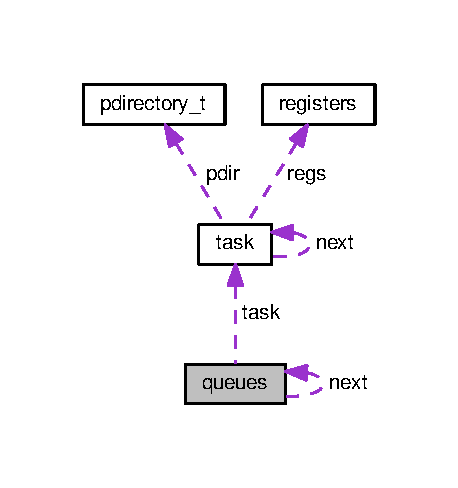
\includegraphics[width=220pt]{structqueues__coll__graph}
\end{center}
\end{figure}
\subsection*{Data Fields}
\begin{DoxyCompactItemize}
\item 
uint32\+\_\+t \hyperlink{structqueues_abcded8e97b078ab04228a84686c301a6}{usage}
\item 
uint32\+\_\+t \hyperlink{structqueues_ab951f1f175f248912a793fc7dac10e5d}{ticks}
\item 
\hyperlink{task_8h_a8aeef2cdb643462b97cd459a8e68cad3}{task\+\_\+t} $\ast$ \hyperlink{structqueues_ad14ef75e56140d0ae658ea2d38d5bb26}{task}
\item 
struct \hyperlink{structqueues}{queues} $\ast$ \hyperlink{structqueues_a9138274fd7864a17d10f7700c2e603d2}{next}
\end{DoxyCompactItemize}


\subsection{Detailed Description}


Definition at line 29 of file task.\+h.



\subsection{Field Documentation}
\index{queues@{queues}!next@{next}}
\index{next@{next}!queues@{queues}}
\subsubsection[{\texorpdfstring{next}{next}}]{\setlength{\rightskip}{0pt plus 5cm}struct {\bf queues}$\ast$ queues\+::next}\hypertarget{structqueues_a9138274fd7864a17d10f7700c2e603d2}{}\label{structqueues_a9138274fd7864a17d10f7700c2e603d2}


Definition at line 33 of file task.\+h.

\index{queues@{queues}!task@{task}}
\index{task@{task}!queues@{queues}}
\subsubsection[{\texorpdfstring{task}{task}}]{\setlength{\rightskip}{0pt plus 5cm}{\bf task\+\_\+t}$\ast$ queues\+::task}\hypertarget{structqueues_ad14ef75e56140d0ae658ea2d38d5bb26}{}\label{structqueues_ad14ef75e56140d0ae658ea2d38d5bb26}


Definition at line 32 of file task.\+h.

\index{queues@{queues}!ticks@{ticks}}
\index{ticks@{ticks}!queues@{queues}}
\subsubsection[{\texorpdfstring{ticks}{ticks}}]{\setlength{\rightskip}{0pt plus 5cm}uint32\+\_\+t queues\+::ticks}\hypertarget{structqueues_ab951f1f175f248912a793fc7dac10e5d}{}\label{structqueues_ab951f1f175f248912a793fc7dac10e5d}


Definition at line 31 of file task.\+h.

\index{queues@{queues}!usage@{usage}}
\index{usage@{usage}!queues@{queues}}
\subsubsection[{\texorpdfstring{usage}{usage}}]{\setlength{\rightskip}{0pt plus 5cm}uint32\+\_\+t queues\+::usage}\hypertarget{structqueues_abcded8e97b078ab04228a84686c301a6}{}\label{structqueues_abcded8e97b078ab04228a84686c301a6}


Definition at line 31 of file task.\+h.



The documentation for this struct was generated from the following file\+:\begin{DoxyCompactItemize}
\item 
Experimental Edition/\+Source/\+Multi\+Tasking/\hyperlink{task_8h}{task.\+h}\end{DoxyCompactItemize}

\hypertarget{structregisters}{}\section{registers Struct Reference}
\label{structregisters}\index{registers@{registers}}


{\ttfamily \#include $<$common.\+h$>$}

\subsection*{Data Fields}
\begin{DoxyCompactItemize}
\item 
uint32\+\_\+t \hyperlink{structregisters_a806ec3ba0cf965d456601aea4c039ec3}{ds}
\item 
uint32\+\_\+t \hyperlink{structregisters_aeedcb447fe6640d43d09c27b7cb8db3b}{edi}
\item 
uint32\+\_\+t \hyperlink{structregisters_a8da011d75d93d36da6c4cf28e1fa3179}{esi}
\item 
uint32\+\_\+t \hyperlink{structregisters_a8d156d1d27fcb1c2f2bbcce1a784431f}{ebp}
\item 
uint32\+\_\+t \hyperlink{structregisters_a9cc3091e4c0f25d142ac74443dc8d384}{esp}
\item 
uint32\+\_\+t \hyperlink{structregisters_aa8989b2fef42dca1d656f724eb324f51}{ebx}
\item 
uint32\+\_\+t \hyperlink{structregisters_af3b40afa73ecdaf2c9279b9ed482d26b}{edx}
\item 
uint32\+\_\+t \hyperlink{structregisters_a00ce491148fd90800c18bd2d4c22e090}{ecx}
\item 
uint32\+\_\+t \hyperlink{structregisters_a1e01e806248cd98e55e0b053db6a6a51}{eax}
\item 
uint32\+\_\+t \hyperlink{structregisters_af311750a9b18afb3b1ed2d144fbe1cb0}{int\+\_\+no}
\item 
uint32\+\_\+t \hyperlink{structregisters_a1f90b3d484c66002c9ffcd0e54e97c2c}{err\+\_\+code}
\item 
uint32\+\_\+t \hyperlink{structregisters_aaeedf83509826a731e436025aeb53576}{eip}
\item 
uint32\+\_\+t \hyperlink{structregisters_a7d73555c87de229a90292640f544ab27}{cs}
\item 
uint32\+\_\+t \hyperlink{structregisters_af9a17981c1cdac71d6f82ba32466a036}{eflags}
\item 
uint32\+\_\+t \hyperlink{structregisters_ad4734529e5faf04f6c61cfabfe4324e9}{useresp}
\item 
uint32\+\_\+t \hyperlink{structregisters_a0da8015246d96b8dcebe98c945fd3d61}{ss}
\end{DoxyCompactItemize}


\subsection{Detailed Description}


Definition at line 72 of file common.\+h.



\subsection{Field Documentation}
\index{registers@{registers}!cs@{cs}}
\index{cs@{cs}!registers@{registers}}
\subsubsection[{\texorpdfstring{cs}{cs}}]{\setlength{\rightskip}{0pt plus 5cm}uint32\+\_\+t registers\+::cs}\hypertarget{structregisters_a7d73555c87de229a90292640f544ab27}{}\label{structregisters_a7d73555c87de229a90292640f544ab27}


Definition at line 77 of file common.\+h.

\index{registers@{registers}!ds@{ds}}
\index{ds@{ds}!registers@{registers}}
\subsubsection[{\texorpdfstring{ds}{ds}}]{\setlength{\rightskip}{0pt plus 5cm}uint32\+\_\+t registers\+::ds}\hypertarget{structregisters_a806ec3ba0cf965d456601aea4c039ec3}{}\label{structregisters_a806ec3ba0cf965d456601aea4c039ec3}


Definition at line 74 of file common.\+h.

\index{registers@{registers}!eax@{eax}}
\index{eax@{eax}!registers@{registers}}
\subsubsection[{\texorpdfstring{eax}{eax}}]{\setlength{\rightskip}{0pt plus 5cm}uint32\+\_\+t registers\+::eax}\hypertarget{structregisters_a1e01e806248cd98e55e0b053db6a6a51}{}\label{structregisters_a1e01e806248cd98e55e0b053db6a6a51}


Definition at line 75 of file common.\+h.

\index{registers@{registers}!ebp@{ebp}}
\index{ebp@{ebp}!registers@{registers}}
\subsubsection[{\texorpdfstring{ebp}{ebp}}]{\setlength{\rightskip}{0pt plus 5cm}uint32\+\_\+t registers\+::ebp}\hypertarget{structregisters_a8d156d1d27fcb1c2f2bbcce1a784431f}{}\label{structregisters_a8d156d1d27fcb1c2f2bbcce1a784431f}


Definition at line 75 of file common.\+h.

\index{registers@{registers}!ebx@{ebx}}
\index{ebx@{ebx}!registers@{registers}}
\subsubsection[{\texorpdfstring{ebx}{ebx}}]{\setlength{\rightskip}{0pt plus 5cm}uint32\+\_\+t registers\+::ebx}\hypertarget{structregisters_aa8989b2fef42dca1d656f724eb324f51}{}\label{structregisters_aa8989b2fef42dca1d656f724eb324f51}


Definition at line 75 of file common.\+h.

\index{registers@{registers}!ecx@{ecx}}
\index{ecx@{ecx}!registers@{registers}}
\subsubsection[{\texorpdfstring{ecx}{ecx}}]{\setlength{\rightskip}{0pt plus 5cm}uint32\+\_\+t registers\+::ecx}\hypertarget{structregisters_a00ce491148fd90800c18bd2d4c22e090}{}\label{structregisters_a00ce491148fd90800c18bd2d4c22e090}


Definition at line 75 of file common.\+h.

\index{registers@{registers}!edi@{edi}}
\index{edi@{edi}!registers@{registers}}
\subsubsection[{\texorpdfstring{edi}{edi}}]{\setlength{\rightskip}{0pt plus 5cm}uint32\+\_\+t registers\+::edi}\hypertarget{structregisters_aeedcb447fe6640d43d09c27b7cb8db3b}{}\label{structregisters_aeedcb447fe6640d43d09c27b7cb8db3b}


Definition at line 75 of file common.\+h.

\index{registers@{registers}!edx@{edx}}
\index{edx@{edx}!registers@{registers}}
\subsubsection[{\texorpdfstring{edx}{edx}}]{\setlength{\rightskip}{0pt plus 5cm}uint32\+\_\+t registers\+::edx}\hypertarget{structregisters_af3b40afa73ecdaf2c9279b9ed482d26b}{}\label{structregisters_af3b40afa73ecdaf2c9279b9ed482d26b}


Definition at line 75 of file common.\+h.

\index{registers@{registers}!eflags@{eflags}}
\index{eflags@{eflags}!registers@{registers}}
\subsubsection[{\texorpdfstring{eflags}{eflags}}]{\setlength{\rightskip}{0pt plus 5cm}uint32\+\_\+t registers\+::eflags}\hypertarget{structregisters_af9a17981c1cdac71d6f82ba32466a036}{}\label{structregisters_af9a17981c1cdac71d6f82ba32466a036}


Definition at line 77 of file common.\+h.

\index{registers@{registers}!eip@{eip}}
\index{eip@{eip}!registers@{registers}}
\subsubsection[{\texorpdfstring{eip}{eip}}]{\setlength{\rightskip}{0pt plus 5cm}uint32\+\_\+t registers\+::eip}\hypertarget{structregisters_aaeedf83509826a731e436025aeb53576}{}\label{structregisters_aaeedf83509826a731e436025aeb53576}


Definition at line 77 of file common.\+h.

\index{registers@{registers}!err\+\_\+code@{err\+\_\+code}}
\index{err\+\_\+code@{err\+\_\+code}!registers@{registers}}
\subsubsection[{\texorpdfstring{err\+\_\+code}{err_code}}]{\setlength{\rightskip}{0pt plus 5cm}uint32\+\_\+t registers\+::err\+\_\+code}\hypertarget{structregisters_a1f90b3d484c66002c9ffcd0e54e97c2c}{}\label{structregisters_a1f90b3d484c66002c9ffcd0e54e97c2c}


Definition at line 76 of file common.\+h.

\index{registers@{registers}!esi@{esi}}
\index{esi@{esi}!registers@{registers}}
\subsubsection[{\texorpdfstring{esi}{esi}}]{\setlength{\rightskip}{0pt plus 5cm}uint32\+\_\+t registers\+::esi}\hypertarget{structregisters_a8da011d75d93d36da6c4cf28e1fa3179}{}\label{structregisters_a8da011d75d93d36da6c4cf28e1fa3179}


Definition at line 75 of file common.\+h.

\index{registers@{registers}!esp@{esp}}
\index{esp@{esp}!registers@{registers}}
\subsubsection[{\texorpdfstring{esp}{esp}}]{\setlength{\rightskip}{0pt plus 5cm}uint32\+\_\+t registers\+::esp}\hypertarget{structregisters_a9cc3091e4c0f25d142ac74443dc8d384}{}\label{structregisters_a9cc3091e4c0f25d142ac74443dc8d384}


Definition at line 75 of file common.\+h.

\index{registers@{registers}!int\+\_\+no@{int\+\_\+no}}
\index{int\+\_\+no@{int\+\_\+no}!registers@{registers}}
\subsubsection[{\texorpdfstring{int\+\_\+no}{int_no}}]{\setlength{\rightskip}{0pt plus 5cm}uint32\+\_\+t registers\+::int\+\_\+no}\hypertarget{structregisters_af311750a9b18afb3b1ed2d144fbe1cb0}{}\label{structregisters_af311750a9b18afb3b1ed2d144fbe1cb0}


Definition at line 76 of file common.\+h.

\index{registers@{registers}!ss@{ss}}
\index{ss@{ss}!registers@{registers}}
\subsubsection[{\texorpdfstring{ss}{ss}}]{\setlength{\rightskip}{0pt plus 5cm}uint32\+\_\+t registers\+::ss}\hypertarget{structregisters_a0da8015246d96b8dcebe98c945fd3d61}{}\label{structregisters_a0da8015246d96b8dcebe98c945fd3d61}


Definition at line 77 of file common.\+h.

\index{registers@{registers}!useresp@{useresp}}
\index{useresp@{useresp}!registers@{registers}}
\subsubsection[{\texorpdfstring{useresp}{useresp}}]{\setlength{\rightskip}{0pt plus 5cm}uint32\+\_\+t registers\+::useresp}\hypertarget{structregisters_ad4734529e5faf04f6c61cfabfe4324e9}{}\label{structregisters_ad4734529e5faf04f6c61cfabfe4324e9}


Definition at line 77 of file common.\+h.



The documentation for this struct was generated from the following file\+:\begin{DoxyCompactItemize}
\item 
Experimental Edition/\+Library/\hyperlink{common_8h}{common.\+h}\end{DoxyCompactItemize}

\hypertarget{structRegisters}{}\section{Registers Struct Reference}
\label{structRegisters}\index{Registers@{Registers}}


{\ttfamily \#include $<$task.\+h$>$}

\subsection*{Data Fields}
\begin{DoxyCompactItemize}
\item 
uint32\+\_\+t \hyperlink{structRegisters_aafc7189a84cb0f6ed3d37ee82bec09bc}{eax}
\item 
uint32\+\_\+t \hyperlink{structRegisters_a3aa9baab41ed6c513cbecb126dc90373}{ebx}
\item 
uint32\+\_\+t \hyperlink{structRegisters_a9a7eb0450238154baa25c72993a0e5e0}{ecx}
\item 
uint32\+\_\+t \hyperlink{structRegisters_a0f90c64246d3bbb917cfe527bf8c34c4}{edx}
\item 
uint32\+\_\+t \hyperlink{structRegisters_a8f9b382cca633127cb869add3aed7a41}{esi}
\item 
uint32\+\_\+t \hyperlink{structRegisters_ae94bf35e0b978f6cca838ec6011a1e48}{edi}
\item 
uint32\+\_\+t \hyperlink{structRegisters_aca352215ac1e37f833da4f6289392261}{esp}
\item 
uint32\+\_\+t \hyperlink{structRegisters_a1e7101b224fc3550bd4b64bb39d83036}{ebp}
\item 
uint32\+\_\+t \hyperlink{structRegisters_ad5110c091e713dabd23f23a62d026c07}{eip}
\item 
uint32\+\_\+t \hyperlink{structRegisters_a5216970c0d34ab4b53881f583839c8f9}{eflags}
\item 
uint32\+\_\+t \hyperlink{structRegisters_ab818d6f237e6d73d321339e6fcd66abf}{cr3}
\end{DoxyCompactItemize}


\subsection{Detailed Description}


Definition at line 11 of file task.\+h.



\subsection{Field Documentation}
\index{Registers@{Registers}!cr3@{cr3}}
\index{cr3@{cr3}!Registers@{Registers}}
\subsubsection[{\texorpdfstring{cr3}{cr3}}]{\setlength{\rightskip}{0pt plus 5cm}uint32\+\_\+t Registers\+::cr3}\hypertarget{structRegisters_ab818d6f237e6d73d321339e6fcd66abf}{}\label{structRegisters_ab818d6f237e6d73d321339e6fcd66abf}


Definition at line 13 of file task.\+h.

\index{Registers@{Registers}!eax@{eax}}
\index{eax@{eax}!Registers@{Registers}}
\subsubsection[{\texorpdfstring{eax}{eax}}]{\setlength{\rightskip}{0pt plus 5cm}uint32\+\_\+t Registers\+::eax}\hypertarget{structRegisters_aafc7189a84cb0f6ed3d37ee82bec09bc}{}\label{structRegisters_aafc7189a84cb0f6ed3d37ee82bec09bc}


Definition at line 13 of file task.\+h.

\index{Registers@{Registers}!ebp@{ebp}}
\index{ebp@{ebp}!Registers@{Registers}}
\subsubsection[{\texorpdfstring{ebp}{ebp}}]{\setlength{\rightskip}{0pt plus 5cm}uint32\+\_\+t Registers\+::ebp}\hypertarget{structRegisters_a1e7101b224fc3550bd4b64bb39d83036}{}\label{structRegisters_a1e7101b224fc3550bd4b64bb39d83036}


Definition at line 13 of file task.\+h.

\index{Registers@{Registers}!ebx@{ebx}}
\index{ebx@{ebx}!Registers@{Registers}}
\subsubsection[{\texorpdfstring{ebx}{ebx}}]{\setlength{\rightskip}{0pt plus 5cm}uint32\+\_\+t Registers\+::ebx}\hypertarget{structRegisters_a3aa9baab41ed6c513cbecb126dc90373}{}\label{structRegisters_a3aa9baab41ed6c513cbecb126dc90373}


Definition at line 13 of file task.\+h.

\index{Registers@{Registers}!ecx@{ecx}}
\index{ecx@{ecx}!Registers@{Registers}}
\subsubsection[{\texorpdfstring{ecx}{ecx}}]{\setlength{\rightskip}{0pt plus 5cm}uint32\+\_\+t Registers\+::ecx}\hypertarget{structRegisters_a9a7eb0450238154baa25c72993a0e5e0}{}\label{structRegisters_a9a7eb0450238154baa25c72993a0e5e0}


Definition at line 13 of file task.\+h.

\index{Registers@{Registers}!edi@{edi}}
\index{edi@{edi}!Registers@{Registers}}
\subsubsection[{\texorpdfstring{edi}{edi}}]{\setlength{\rightskip}{0pt plus 5cm}uint32\+\_\+t Registers\+::edi}\hypertarget{structRegisters_ae94bf35e0b978f6cca838ec6011a1e48}{}\label{structRegisters_ae94bf35e0b978f6cca838ec6011a1e48}


Definition at line 13 of file task.\+h.

\index{Registers@{Registers}!edx@{edx}}
\index{edx@{edx}!Registers@{Registers}}
\subsubsection[{\texorpdfstring{edx}{edx}}]{\setlength{\rightskip}{0pt plus 5cm}uint32\+\_\+t Registers\+::edx}\hypertarget{structRegisters_a0f90c64246d3bbb917cfe527bf8c34c4}{}\label{structRegisters_a0f90c64246d3bbb917cfe527bf8c34c4}


Definition at line 13 of file task.\+h.

\index{Registers@{Registers}!eflags@{eflags}}
\index{eflags@{eflags}!Registers@{Registers}}
\subsubsection[{\texorpdfstring{eflags}{eflags}}]{\setlength{\rightskip}{0pt plus 5cm}uint32\+\_\+t Registers\+::eflags}\hypertarget{structRegisters_a5216970c0d34ab4b53881f583839c8f9}{}\label{structRegisters_a5216970c0d34ab4b53881f583839c8f9}


Definition at line 13 of file task.\+h.

\index{Registers@{Registers}!eip@{eip}}
\index{eip@{eip}!Registers@{Registers}}
\subsubsection[{\texorpdfstring{eip}{eip}}]{\setlength{\rightskip}{0pt plus 5cm}uint32\+\_\+t Registers\+::eip}\hypertarget{structRegisters_ad5110c091e713dabd23f23a62d026c07}{}\label{structRegisters_ad5110c091e713dabd23f23a62d026c07}


Definition at line 13 of file task.\+h.

\index{Registers@{Registers}!esi@{esi}}
\index{esi@{esi}!Registers@{Registers}}
\subsubsection[{\texorpdfstring{esi}{esi}}]{\setlength{\rightskip}{0pt plus 5cm}uint32\+\_\+t Registers\+::esi}\hypertarget{structRegisters_a8f9b382cca633127cb869add3aed7a41}{}\label{structRegisters_a8f9b382cca633127cb869add3aed7a41}


Definition at line 13 of file task.\+h.

\index{Registers@{Registers}!esp@{esp}}
\index{esp@{esp}!Registers@{Registers}}
\subsubsection[{\texorpdfstring{esp}{esp}}]{\setlength{\rightskip}{0pt plus 5cm}uint32\+\_\+t Registers\+::esp}\hypertarget{structRegisters_aca352215ac1e37f833da4f6289392261}{}\label{structRegisters_aca352215ac1e37f833da4f6289392261}


Definition at line 13 of file task.\+h.



The documentation for this struct was generated from the following file\+:\begin{DoxyCompactItemize}
\item 
Experimental Edition/\+Source/\+Multi\+Tasking/\hyperlink{task_8h}{task.\+h}\end{DoxyCompactItemize}

\hypertarget{structregs}{}\section{regs Struct Reference}
\label{structregs}\index{regs@{regs}}


{\ttfamily \#include $<$system.\+h$>$}

\subsection*{Data Fields}
\begin{DoxyCompactItemize}
\item 
unsigned int \hyperlink{structregs_a65174883574b177d940de50d85d000ea}{gs}
\item 
unsigned int \hyperlink{structregs_a0a3292601916fad9c8e8463d5466652d}{fs}
\item 
unsigned int \hyperlink{structregs_a8a3e5cd6d92486294b5bdda1963fde40}{es}
\item 
unsigned int \hyperlink{structregs_a11ee12613bc58244d6e3b166e1892f4a}{ds}
\item 
unsigned int \hyperlink{structregs_a273e21e568ee550e48dfc2799e5e7d56}{edi}
\item 
unsigned int \hyperlink{structregs_ab25239e8d63dfa05c9ad2f2ba4a0ff7a}{esi}
\item 
unsigned int \hyperlink{structregs_a27936092be139fd35a48fbcf6d3cc318}{ebp}
\item 
unsigned int \hyperlink{structregs_a6671599aa5e59fd804561c1c1ed7c53a}{esp}
\item 
unsigned int \hyperlink{structregs_a1d732c32ac0bd3f2c0a1b84fed7b6312}{ebx}
\item 
unsigned int \hyperlink{structregs_a5177b6604bc2937159c29899a0a6b94a}{edx}
\item 
unsigned int \hyperlink{structregs_a32f7d03f98565974abed738eee025e62}{ecx}
\item 
unsigned int \hyperlink{structregs_af3ee7124e26955c62234c23ff7420fa5}{eax}
\item 
unsigned int \hyperlink{structregs_a0447d192cd01c7958fc5e06746c345d9}{int\+\_\+no}
\item 
unsigned int \hyperlink{structregs_a37177085b61efd8c7d777880ed814ffe}{err\+\_\+code}
\item 
unsigned int \hyperlink{structregs_a483d469ae6b388e4df869c1ebd61d713}{eip}
\item 
unsigned int \hyperlink{structregs_a178d60c6cd2b033533d4a35b966e8868}{cs}
\item 
unsigned int \hyperlink{structregs_a2394860816e82786acb64671237492b2}{eflags}
\item 
unsigned int \hyperlink{structregs_a55d3b6b0025dd401f204d585d256c140}{useresp}
\item 
unsigned int \hyperlink{structregs_ae24c40e9efb433989445bfd318564c90}{ss}
\end{DoxyCompactItemize}


\subsection{Detailed Description}


Definition at line 22 of file system.\+h.



\subsection{Field Documentation}
\index{regs@{regs}!cs@{cs}}
\index{cs@{cs}!regs@{regs}}
\subsubsection[{\texorpdfstring{cs}{cs}}]{\setlength{\rightskip}{0pt plus 5cm}unsigned int regs\+::cs}\hypertarget{structregs_a178d60c6cd2b033533d4a35b966e8868}{}\label{structregs_a178d60c6cd2b033533d4a35b966e8868}


Definition at line 27 of file system.\+h.

\index{regs@{regs}!ds@{ds}}
\index{ds@{ds}!regs@{regs}}
\subsubsection[{\texorpdfstring{ds}{ds}}]{\setlength{\rightskip}{0pt plus 5cm}unsigned int regs\+::ds}\hypertarget{structregs_a11ee12613bc58244d6e3b166e1892f4a}{}\label{structregs_a11ee12613bc58244d6e3b166e1892f4a}


Definition at line 24 of file system.\+h.

\index{regs@{regs}!eax@{eax}}
\index{eax@{eax}!regs@{regs}}
\subsubsection[{\texorpdfstring{eax}{eax}}]{\setlength{\rightskip}{0pt plus 5cm}unsigned int regs\+::eax}\hypertarget{structregs_af3ee7124e26955c62234c23ff7420fa5}{}\label{structregs_af3ee7124e26955c62234c23ff7420fa5}


Definition at line 25 of file system.\+h.

\index{regs@{regs}!ebp@{ebp}}
\index{ebp@{ebp}!regs@{regs}}
\subsubsection[{\texorpdfstring{ebp}{ebp}}]{\setlength{\rightskip}{0pt plus 5cm}unsigned int regs\+::ebp}\hypertarget{structregs_a27936092be139fd35a48fbcf6d3cc318}{}\label{structregs_a27936092be139fd35a48fbcf6d3cc318}


Definition at line 25 of file system.\+h.

\index{regs@{regs}!ebx@{ebx}}
\index{ebx@{ebx}!regs@{regs}}
\subsubsection[{\texorpdfstring{ebx}{ebx}}]{\setlength{\rightskip}{0pt plus 5cm}unsigned int regs\+::ebx}\hypertarget{structregs_a1d732c32ac0bd3f2c0a1b84fed7b6312}{}\label{structregs_a1d732c32ac0bd3f2c0a1b84fed7b6312}


Definition at line 25 of file system.\+h.

\index{regs@{regs}!ecx@{ecx}}
\index{ecx@{ecx}!regs@{regs}}
\subsubsection[{\texorpdfstring{ecx}{ecx}}]{\setlength{\rightskip}{0pt plus 5cm}unsigned int regs\+::ecx}\hypertarget{structregs_a32f7d03f98565974abed738eee025e62}{}\label{structregs_a32f7d03f98565974abed738eee025e62}


Definition at line 25 of file system.\+h.

\index{regs@{regs}!edi@{edi}}
\index{edi@{edi}!regs@{regs}}
\subsubsection[{\texorpdfstring{edi}{edi}}]{\setlength{\rightskip}{0pt plus 5cm}unsigned int regs\+::edi}\hypertarget{structregs_a273e21e568ee550e48dfc2799e5e7d56}{}\label{structregs_a273e21e568ee550e48dfc2799e5e7d56}


Definition at line 25 of file system.\+h.

\index{regs@{regs}!edx@{edx}}
\index{edx@{edx}!regs@{regs}}
\subsubsection[{\texorpdfstring{edx}{edx}}]{\setlength{\rightskip}{0pt plus 5cm}unsigned int regs\+::edx}\hypertarget{structregs_a5177b6604bc2937159c29899a0a6b94a}{}\label{structregs_a5177b6604bc2937159c29899a0a6b94a}


Definition at line 25 of file system.\+h.

\index{regs@{regs}!eflags@{eflags}}
\index{eflags@{eflags}!regs@{regs}}
\subsubsection[{\texorpdfstring{eflags}{eflags}}]{\setlength{\rightskip}{0pt plus 5cm}unsigned int regs\+::eflags}\hypertarget{structregs_a2394860816e82786acb64671237492b2}{}\label{structregs_a2394860816e82786acb64671237492b2}


Definition at line 27 of file system.\+h.

\index{regs@{regs}!eip@{eip}}
\index{eip@{eip}!regs@{regs}}
\subsubsection[{\texorpdfstring{eip}{eip}}]{\setlength{\rightskip}{0pt plus 5cm}unsigned int regs\+::eip}\hypertarget{structregs_a483d469ae6b388e4df869c1ebd61d713}{}\label{structregs_a483d469ae6b388e4df869c1ebd61d713}


Definition at line 27 of file system.\+h.

\index{regs@{regs}!err\+\_\+code@{err\+\_\+code}}
\index{err\+\_\+code@{err\+\_\+code}!regs@{regs}}
\subsubsection[{\texorpdfstring{err\+\_\+code}{err_code}}]{\setlength{\rightskip}{0pt plus 5cm}unsigned int regs\+::err\+\_\+code}\hypertarget{structregs_a37177085b61efd8c7d777880ed814ffe}{}\label{structregs_a37177085b61efd8c7d777880ed814ffe}


Definition at line 26 of file system.\+h.

\index{regs@{regs}!es@{es}}
\index{es@{es}!regs@{regs}}
\subsubsection[{\texorpdfstring{es}{es}}]{\setlength{\rightskip}{0pt plus 5cm}unsigned int regs\+::es}\hypertarget{structregs_a8a3e5cd6d92486294b5bdda1963fde40}{}\label{structregs_a8a3e5cd6d92486294b5bdda1963fde40}


Definition at line 24 of file system.\+h.

\index{regs@{regs}!esi@{esi}}
\index{esi@{esi}!regs@{regs}}
\subsubsection[{\texorpdfstring{esi}{esi}}]{\setlength{\rightskip}{0pt plus 5cm}unsigned int regs\+::esi}\hypertarget{structregs_ab25239e8d63dfa05c9ad2f2ba4a0ff7a}{}\label{structregs_ab25239e8d63dfa05c9ad2f2ba4a0ff7a}


Definition at line 25 of file system.\+h.

\index{regs@{regs}!esp@{esp}}
\index{esp@{esp}!regs@{regs}}
\subsubsection[{\texorpdfstring{esp}{esp}}]{\setlength{\rightskip}{0pt plus 5cm}unsigned int regs\+::esp}\hypertarget{structregs_a6671599aa5e59fd804561c1c1ed7c53a}{}\label{structregs_a6671599aa5e59fd804561c1c1ed7c53a}


Definition at line 25 of file system.\+h.

\index{regs@{regs}!fs@{fs}}
\index{fs@{fs}!regs@{regs}}
\subsubsection[{\texorpdfstring{fs}{fs}}]{\setlength{\rightskip}{0pt plus 5cm}unsigned int regs\+::fs}\hypertarget{structregs_a0a3292601916fad9c8e8463d5466652d}{}\label{structregs_a0a3292601916fad9c8e8463d5466652d}


Definition at line 24 of file system.\+h.

\index{regs@{regs}!gs@{gs}}
\index{gs@{gs}!regs@{regs}}
\subsubsection[{\texorpdfstring{gs}{gs}}]{\setlength{\rightskip}{0pt plus 5cm}unsigned int regs\+::gs}\hypertarget{structregs_a65174883574b177d940de50d85d000ea}{}\label{structregs_a65174883574b177d940de50d85d000ea}


Definition at line 24 of file system.\+h.

\index{regs@{regs}!int\+\_\+no@{int\+\_\+no}}
\index{int\+\_\+no@{int\+\_\+no}!regs@{regs}}
\subsubsection[{\texorpdfstring{int\+\_\+no}{int_no}}]{\setlength{\rightskip}{0pt plus 5cm}unsigned int regs\+::int\+\_\+no}\hypertarget{structregs_a0447d192cd01c7958fc5e06746c345d9}{}\label{structregs_a0447d192cd01c7958fc5e06746c345d9}


Definition at line 26 of file system.\+h.

\index{regs@{regs}!ss@{ss}}
\index{ss@{ss}!regs@{regs}}
\subsubsection[{\texorpdfstring{ss}{ss}}]{\setlength{\rightskip}{0pt plus 5cm}unsigned int regs\+::ss}\hypertarget{structregs_ae24c40e9efb433989445bfd318564c90}{}\label{structregs_ae24c40e9efb433989445bfd318564c90}


Definition at line 27 of file system.\+h.

\index{regs@{regs}!useresp@{useresp}}
\index{useresp@{useresp}!regs@{regs}}
\subsubsection[{\texorpdfstring{useresp}{useresp}}]{\setlength{\rightskip}{0pt plus 5cm}unsigned int regs\+::useresp}\hypertarget{structregs_a55d3b6b0025dd401f204d585d256c140}{}\label{structregs_a55d3b6b0025dd401f204d585d256c140}


Definition at line 27 of file system.\+h.



The documentation for this struct was generated from the following file\+:\begin{DoxyCompactItemize}
\item 
Experimental Edition/\+Library/\hyperlink{system_8h}{system.\+h}\end{DoxyCompactItemize}

\hypertarget{structRSDPtr}{}\section{R\+S\+D\+Ptr Struct Reference}
\label{structRSDPtr}\index{R\+S\+D\+Ptr@{R\+S\+D\+Ptr}}
\subsection*{Data Fields}
\begin{DoxyCompactItemize}
\item 
\hyperlink{acpi_8c_a0c8186d9b9b7880309c27230bbb5e69d}{byte} \hyperlink{structRSDPtr_ae3efa3d06b7688110654bd24df504270}{Signature} \mbox{[}8\mbox{]}
\item 
\hyperlink{acpi_8c_a0c8186d9b9b7880309c27230bbb5e69d}{byte} \hyperlink{structRSDPtr_a97114fb497c50827e574cc983548073d}{Check\+Sum}
\item 
\hyperlink{acpi_8c_a0c8186d9b9b7880309c27230bbb5e69d}{byte} \hyperlink{structRSDPtr_abdc8155e2acf415b30213793e4875306}{Oem\+ID} \mbox{[}6\mbox{]}
\item 
\hyperlink{acpi_8c_a0c8186d9b9b7880309c27230bbb5e69d}{byte} \hyperlink{structRSDPtr_aa7a0f77fcedb849e6a3d5eb68a5df4cb}{Revision}
\item 
\hyperlink{acpi_8c_a74cb93d430006e784da73b8ca406ee6e}{dword} $\ast$ \hyperlink{structRSDPtr_a982825bea34910320148af4114ba8e00}{Rsdt\+Address}
\end{DoxyCompactItemize}


\subsection{Detailed Description}


Definition at line 25 of file acpi.\+c.



\subsection{Field Documentation}
\index{R\+S\+D\+Ptr@{R\+S\+D\+Ptr}!Check\+Sum@{Check\+Sum}}
\index{Check\+Sum@{Check\+Sum}!R\+S\+D\+Ptr@{R\+S\+D\+Ptr}}
\subsubsection[{\texorpdfstring{Check\+Sum}{CheckSum}}]{\setlength{\rightskip}{0pt plus 5cm}{\bf byte} R\+S\+D\+Ptr\+::\+Check\+Sum}\hypertarget{structRSDPtr_a97114fb497c50827e574cc983548073d}{}\label{structRSDPtr_a97114fb497c50827e574cc983548073d}


Definition at line 28 of file acpi.\+c.

\index{R\+S\+D\+Ptr@{R\+S\+D\+Ptr}!Oem\+ID@{Oem\+ID}}
\index{Oem\+ID@{Oem\+ID}!R\+S\+D\+Ptr@{R\+S\+D\+Ptr}}
\subsubsection[{\texorpdfstring{Oem\+ID}{OemID}}]{\setlength{\rightskip}{0pt plus 5cm}{\bf byte} R\+S\+D\+Ptr\+::\+Oem\+ID\mbox{[}6\mbox{]}}\hypertarget{structRSDPtr_abdc8155e2acf415b30213793e4875306}{}\label{structRSDPtr_abdc8155e2acf415b30213793e4875306}


Definition at line 29 of file acpi.\+c.

\index{R\+S\+D\+Ptr@{R\+S\+D\+Ptr}!Revision@{Revision}}
\index{Revision@{Revision}!R\+S\+D\+Ptr@{R\+S\+D\+Ptr}}
\subsubsection[{\texorpdfstring{Revision}{Revision}}]{\setlength{\rightskip}{0pt plus 5cm}{\bf byte} R\+S\+D\+Ptr\+::\+Revision}\hypertarget{structRSDPtr_aa7a0f77fcedb849e6a3d5eb68a5df4cb}{}\label{structRSDPtr_aa7a0f77fcedb849e6a3d5eb68a5df4cb}


Definition at line 30 of file acpi.\+c.

\index{R\+S\+D\+Ptr@{R\+S\+D\+Ptr}!Rsdt\+Address@{Rsdt\+Address}}
\index{Rsdt\+Address@{Rsdt\+Address}!R\+S\+D\+Ptr@{R\+S\+D\+Ptr}}
\subsubsection[{\texorpdfstring{Rsdt\+Address}{RsdtAddress}}]{\setlength{\rightskip}{0pt plus 5cm}{\bf dword}$\ast$ R\+S\+D\+Ptr\+::\+Rsdt\+Address}\hypertarget{structRSDPtr_a982825bea34910320148af4114ba8e00}{}\label{structRSDPtr_a982825bea34910320148af4114ba8e00}


Definition at line 31 of file acpi.\+c.

\index{R\+S\+D\+Ptr@{R\+S\+D\+Ptr}!Signature@{Signature}}
\index{Signature@{Signature}!R\+S\+D\+Ptr@{R\+S\+D\+Ptr}}
\subsubsection[{\texorpdfstring{Signature}{Signature}}]{\setlength{\rightskip}{0pt plus 5cm}{\bf byte} R\+S\+D\+Ptr\+::\+Signature\mbox{[}8\mbox{]}}\hypertarget{structRSDPtr_ae3efa3d06b7688110654bd24df504270}{}\label{structRSDPtr_ae3efa3d06b7688110654bd24df504270}


Definition at line 27 of file acpi.\+c.



The documentation for this struct was generated from the following file\+:\begin{DoxyCompactItemize}
\item 
Experimental Edition/\+Source/\+Drivers/\+A\+C\+P\+I/\hyperlink{acpi_8c}{acpi.\+c}\end{DoxyCompactItemize}

\hypertarget{structSATA__ident}{}\section{S\+A\+T\+A\+\_\+ident Struct Reference}
\label{structSATA__ident}\index{S\+A\+T\+A\+\_\+ident@{S\+A\+T\+A\+\_\+ident}}


{\ttfamily \#include $<$ahci.\+h$>$}

\subsection*{Data Fields}
\begin{DoxyCompactItemize}
\item 
unsigned short \hyperlink{structSATA__ident_a3e2eb6859b4845ab26956b03933e8774}{config}
\item 
unsigned short \hyperlink{structSATA__ident_a4ecef9e7e7c21adcd2cdbbb6947074f7}{cyls}
\item 
unsigned short \hyperlink{structSATA__ident_a8be69794eccacf473f7c55523dfdd885}{reserved2}
\item 
unsigned short \hyperlink{structSATA__ident_a3e5cda071ccaf6040395b709b17af752}{heads}
\item 
unsigned short \hyperlink{structSATA__ident_afc42e0fec367087ac600bf1eee537efb}{track\+\_\+bytes}
\item 
unsigned short \hyperlink{structSATA__ident_a586fe0828c423dac3306683c0b275a35}{sector\+\_\+bytes}
\item 
unsigned short \hyperlink{structSATA__ident_ad3a035c565a78ea9fafaf696ab2e29b8}{sectors}
\item 
unsigned short \hyperlink{structSATA__ident_a59ae424a72fd8d4ccb2eec8b94f97dd1}{vendor0}
\item 
unsigned short \hyperlink{structSATA__ident_a57a0bd1026214ec3cad61717fea08ee9}{vendor1}
\item 
unsigned short \hyperlink{structSATA__ident_a7c5a4057f43da3eff3935c977d634a0d}{vendor2}
\item 
unsigned char \hyperlink{structSATA__ident_ab3928623c2c1f05d7dd0635aef68adf7}{serial\+\_\+no} \mbox{[}20\mbox{]}
\item 
unsigned short \hyperlink{structSATA__ident_a697bedabe956a0d4022ef9c2aca00c97}{buf\+\_\+type}
\item 
unsigned short \hyperlink{structSATA__ident_a775f5fa54b6bcb76cc9f93a38bd09c99}{buf\+\_\+size}
\item 
unsigned short \hyperlink{structSATA__ident_a09bad065c4b053be42711ffd161fbed7}{ecc\+\_\+bytes}
\item 
unsigned char \hyperlink{structSATA__ident_a083cc6c6f2a7728709aff9726f8c6913}{fw\+\_\+rev} \mbox{[}8\mbox{]}
\item 
unsigned char \hyperlink{structSATA__ident_a2a36d687174ca2eebc0587eb0882e89f}{model} \mbox{[}40\mbox{]}
\item 
unsigned short \hyperlink{structSATA__ident_ae4fad74cecade33dc2e3e24756eba3d6}{multi\+\_\+count}
\item 
unsigned short \hyperlink{structSATA__ident_a7399191120ad754a14ea722897e7d29a}{dword\+\_\+io}
\item 
unsigned short \hyperlink{structSATA__ident_a31f63a30e501d36ba2f2c5ccf573a51e}{capability1}
\item 
unsigned short \hyperlink{structSATA__ident_a0dffaaa0f1a60b51faf00a3ca2c993ac}{capability2}
\item 
unsigned char \hyperlink{structSATA__ident_ab565f3b27395b9d783a6c1a5752c1090}{vendor5}
\item 
unsigned char \hyperlink{structSATA__ident_abf328a06ef3d38cbde3b259c09504510}{t\+P\+IO}
\item 
unsigned char \hyperlink{structSATA__ident_ab39d63c6a76245c7b33ae8bdf0928859}{vendor6}
\item 
unsigned char \hyperlink{structSATA__ident_af4ac3e7711b35ed8bc6989d23d914b36}{t\+D\+MA}
\item 
unsigned short \hyperlink{structSATA__ident_a608cd51a438131e344a202ffc559c9b6}{field\+\_\+valid}
\item 
unsigned short \hyperlink{structSATA__ident_a5e404662579618edbd9f77571365a993}{cur\+\_\+cyls}
\item 
unsigned short \hyperlink{structSATA__ident_a1fe29be2e7d4c125e53a63297e7d6041}{cur\+\_\+heads}
\item 
unsigned short \hyperlink{structSATA__ident_add99ae85cb8e599a0344fbc72787c707}{cur\+\_\+sectors}
\item 
unsigned short \hyperlink{structSATA__ident_af99cde338deece51a862fd3df0732d16}{cur\+\_\+capacity0}
\item 
unsigned short \hyperlink{structSATA__ident_ae00faf5e261fb84c826a7862c255e6c2}{cur\+\_\+capacity1}
\item 
unsigned char \hyperlink{structSATA__ident_ab259130c7d5a5032eabf063e63a823e8}{multsect}
\item 
unsigned char \hyperlink{structSATA__ident_a4b96a867298b90fe2bc53cb295b8eaf6}{multsect\+\_\+valid}
\item 
unsigned int \hyperlink{structSATA__ident_acd8bcb50bbcde8afa6b790e733569563}{lba\+\_\+capacity}
\item 
unsigned short \hyperlink{structSATA__ident_a5a7cbcc17497c2cb6bfc6a79c7bca798}{dma\+\_\+1word}
\item 
unsigned short \hyperlink{structSATA__ident_a3baea9abdcd9f21814c53094b1037f43}{dma\+\_\+mword}
\item 
unsigned short \hyperlink{structSATA__ident_ae833370217f85d6eaafd82f290cfebd4}{eide\+\_\+pio\+\_\+modes}
\item 
unsigned short \hyperlink{structSATA__ident_a298cef7737e82b93d37c519b06fe3d37}{eide\+\_\+dma\+\_\+min}
\item 
unsigned short \hyperlink{structSATA__ident_a63768c1ba04a1ca34944e34cbf4239fa}{eide\+\_\+dma\+\_\+time}
\item 
unsigned short \hyperlink{structSATA__ident_a4a56a283b3953bbf7319c35b6ef38654}{eide\+\_\+pio}
\item 
unsigned short \hyperlink{structSATA__ident_a884661c28a77066fb1968a432a48dc80}{eide\+\_\+pio\+\_\+iordy}
\item 
unsigned short \hyperlink{structSATA__ident_a92889f3e742cf5d85af65e26a83701c0}{words69\+\_\+70} \mbox{[}2\mbox{]}
\item 
unsigned short \hyperlink{structSATA__ident_a6cc31fab7053c53b3797051c0d9013a8}{words71\+\_\+74} \mbox{[}4\mbox{]}
\item 
unsigned short \hyperlink{structSATA__ident_adcc438f4fea20d3923975c215a3b4bdb}{queue\+\_\+depth}
\item 
unsigned short \hyperlink{structSATA__ident_aa8bd934743b5ee069527b69a0b03d0a0}{sata\+\_\+capability}
\item 
unsigned short \hyperlink{structSATA__ident_ac397fd6793b8efa1f3e3c743ae3ab8d6}{sata\+\_\+additional}
\item 
unsigned short \hyperlink{structSATA__ident_abbd1fd98f82be0ce8e3278f63065f886}{sata\+\_\+supported}
\item 
unsigned short \hyperlink{structSATA__ident_aff86049b3b642c906338107dd9a72578}{features\+\_\+enabled}
\item 
unsigned short \hyperlink{structSATA__ident_a20072f19c069ac7fd06c1b1b35cac9cf}{major\+\_\+rev\+\_\+num}
\item 
unsigned short \hyperlink{structSATA__ident_a43a70eb59b8388d13f79d3b02b0a7c51}{minor\+\_\+rev\+\_\+num}
\item 
unsigned short \hyperlink{structSATA__ident_af94e7c7a492cbcd4586315ffea27076a}{command\+\_\+set\+\_\+1}
\item 
unsigned short \hyperlink{structSATA__ident_a2392729304479e06e003afc3578b3b34}{command\+\_\+set\+\_\+2}
\item 
unsigned short \hyperlink{structSATA__ident_a9d98244646733dfe714c46d0e8a58ecd}{cfsse}
\item 
unsigned short \hyperlink{structSATA__ident_acb6d9e0d24967112a83d6e195f77469a}{cfs\+\_\+enable\+\_\+1}
\item 
unsigned short \hyperlink{structSATA__ident_af76747e91afd940fbe5c4c05ee0b6396}{cfs\+\_\+enable\+\_\+2}
\item 
unsigned short \hyperlink{structSATA__ident_ab29fc72ea1317ab5f5d06d59ab7b84ff}{csf\+\_\+default}
\item 
unsigned short \hyperlink{structSATA__ident_a16f42ed6bf33839490b8684e77801f41}{dma\+\_\+ultra}
\item 
unsigned short \hyperlink{structSATA__ident_ac3c1a0f34c6c77762de11b4a1995914a}{word89}
\item 
unsigned short \hyperlink{structSATA__ident_a2c2baf9509a80f36e4e1ac4767937005}{word90}
\item 
unsigned short \hyperlink{structSATA__ident_a54577593de0dd4e949ad36a746325af0}{Cur\+A\+P\+Mvalues}
\item 
unsigned short \hyperlink{structSATA__ident_a8fb2a1e3cc82865443fa41f666ebe88b}{word92}
\item 
unsigned short \hyperlink{structSATA__ident_a6498b61fb0529b5e774dd2f633ea5fe6}{comreset}
\item 
unsigned short \hyperlink{structSATA__ident_ab35db051cb2210e01f0a316e61b90c76}{accoustic}
\item 
unsigned short \hyperlink{structSATA__ident_adbb9bf7c54a82fb330df2fd2bc58ded9}{min\+\_\+req\+\_\+sz}
\item 
unsigned short \hyperlink{structSATA__ident_a5b0a4388fb4ed0a5d087053c492ac6e8}{transfer\+\_\+time\+\_\+dma}
\item 
unsigned short \hyperlink{structSATA__ident_ab0d4a28726318540f1a23cb47e71a682}{access\+\_\+latency}
\item 
unsigned int \hyperlink{structSATA__ident_a6497132c3ec773dfe63a6d9e671bcd6b}{perf\+\_\+granularity}
\item 
unsigned int \hyperlink{structSATA__ident_a37e147644b63060f56f12605f8578441}{total\+\_\+usr\+\_\+sectors} \mbox{[}2\mbox{]}
\item 
unsigned short \hyperlink{structSATA__ident_a39b24989e9dc3b2c7c09434f64318cbf}{transfer\+\_\+time\+\_\+pio}
\item 
unsigned short \hyperlink{structSATA__ident_abf5b445f2faecb276859b5c8c7b7a5e6}{reserved105}
\item 
unsigned short \hyperlink{structSATA__ident_a36c839a543d3bc8ae5cc834591d0fda2}{sector\+\_\+sz}
\item 
unsigned short \hyperlink{structSATA__ident_a6d2b3ab59e6b5a3914cfc775ac7a273b}{inter\+\_\+seek\+\_\+delay}
\item 
unsigned short \hyperlink{structSATA__ident_a11cabfdf0f71c170262978bb08445d3a}{words108\+\_\+116} \mbox{[}9\mbox{]}
\item 
unsigned int \hyperlink{structSATA__ident_a0c0d441c5e9cfd17d9dfa69c102ecafd}{words\+\_\+per\+\_\+sector}
\item 
unsigned short \hyperlink{structSATA__ident_ae8dec1fde7e95fc8810c1fc1a3849eff}{supported\+\_\+settings}
\item 
unsigned short \hyperlink{structSATA__ident_a8e97ec892f9b34e03fd3e118232cb33d}{command\+\_\+set\+\_\+3}
\item 
unsigned short \hyperlink{structSATA__ident_a50b9d23ab1fe7bd099651c205b273ddc}{words121\+\_\+126} \mbox{[}6\mbox{]}
\item 
unsigned short \hyperlink{structSATA__ident_a0304f0c077add497b87185216200fca1}{word127}
\item 
unsigned short \hyperlink{structSATA__ident_a103941b9ece90ff1df2c58e2fa2866d7}{security\+\_\+status}
\item 
unsigned short \hyperlink{structSATA__ident_a1ccb2068f8fe097ee7055f214b1f8416}{csfo}
\item 
unsigned short \hyperlink{structSATA__ident_ab65ec26c6dc0d14d5c7bd8981ec68d74}{words130\+\_\+155} \mbox{[}26\mbox{]}
\item 
unsigned short \hyperlink{structSATA__ident_a56ba76f0701ac2544a8b69a54360915f}{word156}
\item 
unsigned short \hyperlink{structSATA__ident_a0ee80af77570613f9ba08c1bd30a90d5}{words157\+\_\+159} \mbox{[}3\mbox{]}
\item 
unsigned short \hyperlink{structSATA__ident_a73387dc40b352ee650bd1a5875849e08}{cfa}
\item 
unsigned short \hyperlink{structSATA__ident_a876fd52ee84beddb2b5e9a1a99ce098e}{words161\+\_\+175} \mbox{[}15\mbox{]}
\item 
unsigned char \hyperlink{structSATA__ident_a20fa3859f2745ac5a2f32cb5d5a6ed62}{media\+\_\+serial} \mbox{[}60\mbox{]}
\item 
unsigned short \hyperlink{structSATA__ident_ae181871bbc156f78608cb240648b113a}{sct\+\_\+cmd\+\_\+transport}
\item 
unsigned short \hyperlink{structSATA__ident_a6d22ea8ccce917853c3558482d51c2ad}{words207\+\_\+208} \mbox{[}2\mbox{]}
\item 
unsigned short \hyperlink{structSATA__ident_a7d3d9ee177c7fbdf752d10c4df81ce9f}{block\+\_\+align}
\item 
unsigned int \hyperlink{structSATA__ident_a9666dd870fe2ef49ea21adb0b897022d}{W\+R\+V\+\_\+sec\+\_\+count}
\item 
unsigned int \hyperlink{structSATA__ident_ac94f9f7b192f2f636310b6718d752aea}{verf\+\_\+sec\+\_\+count}
\item 
unsigned short \hyperlink{structSATA__ident_ad1ca0009d9c3bb07fc592074c4d0fa71}{nv\+\_\+cache\+\_\+capability}
\item 
unsigned short \hyperlink{structSATA__ident_a0a2b0b5c33bf357f681b9c96f82ac845}{nv\+\_\+cache\+\_\+sz}
\item 
unsigned short \hyperlink{structSATA__ident_a3d5a99c03cd6d648e743734cb5982f8d}{nv\+\_\+cache\+\_\+sz2}
\item 
unsigned short \hyperlink{structSATA__ident_ab28e705ed0d36775a4782ee4d5c37899}{rotation\+\_\+rate}
\item 
unsigned short \hyperlink{structSATA__ident_a06e5d3fdae8830492b2a8360a229f8d4}{reserved218}
\item 
unsigned short \hyperlink{structSATA__ident_a1cc18559fb89be13ccce7858162049b4}{nv\+\_\+cache\+\_\+options}
\item 
unsigned short \hyperlink{structSATA__ident_aa7710925f1b4b459e6499ce2d3e82408}{words220\+\_\+221} \mbox{[}2\mbox{]}
\item 
unsigned short \hyperlink{structSATA__ident_ae04d840fdf1a87cc832b491a0e02ee0c}{transport\+\_\+major\+\_\+rev}
\item 
unsigned short \hyperlink{structSATA__ident_a582e9c9d3e52b0f84a4b311c48aaa2b5}{transport\+\_\+minor\+\_\+rev}
\item 
unsigned short \hyperlink{structSATA__ident_a1b7fe4d0ce0792c7d6e0c5b3ecfa7063}{words224\+\_\+233} \mbox{[}10\mbox{]}
\item 
unsigned short \hyperlink{structSATA__ident_aad38263481e1b39593f8a381a072b170}{min\+\_\+dwnload\+\_\+blocks}
\item 
unsigned short \hyperlink{structSATA__ident_a93c778d7e7521c8e84682c52c8e5dc6e}{max\+\_\+dwnload\+\_\+blocks}
\item 
unsigned short \hyperlink{structSATA__ident_ab3312fab93f9e413abe360b4a1823c7b}{words236\+\_\+254} \mbox{[}19\mbox{]}
\item 
unsigned short \hyperlink{structSATA__ident_a9bbddec56882e46f0385cea68e3d9f4c}{integrity}
\end{DoxyCompactItemize}


\subsection{Detailed Description}


Definition at line 502 of file ahci.\+h.



\subsection{Field Documentation}
\index{S\+A\+T\+A\+\_\+ident@{S\+A\+T\+A\+\_\+ident}!access\+\_\+latency@{access\+\_\+latency}}
\index{access\+\_\+latency@{access\+\_\+latency}!S\+A\+T\+A\+\_\+ident@{S\+A\+T\+A\+\_\+ident}}
\subsubsection[{\texorpdfstring{access\+\_\+latency}{access_latency}}]{\setlength{\rightskip}{0pt plus 5cm}unsigned short S\+A\+T\+A\+\_\+ident\+::access\+\_\+latency}\hypertarget{structSATA__ident_ab0d4a28726318540f1a23cb47e71a682}{}\label{structSATA__ident_ab0d4a28726318540f1a23cb47e71a682}


Definition at line 568 of file ahci.\+h.

\index{S\+A\+T\+A\+\_\+ident@{S\+A\+T\+A\+\_\+ident}!accoustic@{accoustic}}
\index{accoustic@{accoustic}!S\+A\+T\+A\+\_\+ident@{S\+A\+T\+A\+\_\+ident}}
\subsubsection[{\texorpdfstring{accoustic}{accoustic}}]{\setlength{\rightskip}{0pt plus 5cm}unsigned short S\+A\+T\+A\+\_\+ident\+::accoustic}\hypertarget{structSATA__ident_ab35db051cb2210e01f0a316e61b90c76}{}\label{structSATA__ident_ab35db051cb2210e01f0a316e61b90c76}


Definition at line 565 of file ahci.\+h.

\index{S\+A\+T\+A\+\_\+ident@{S\+A\+T\+A\+\_\+ident}!block\+\_\+align@{block\+\_\+align}}
\index{block\+\_\+align@{block\+\_\+align}!S\+A\+T\+A\+\_\+ident@{S\+A\+T\+A\+\_\+ident}}
\subsubsection[{\texorpdfstring{block\+\_\+align}{block_align}}]{\setlength{\rightskip}{0pt plus 5cm}unsigned short S\+A\+T\+A\+\_\+ident\+::block\+\_\+align}\hypertarget{structSATA__ident_a7d3d9ee177c7fbdf752d10c4df81ce9f}{}\label{structSATA__ident_a7d3d9ee177c7fbdf752d10c4df81ce9f}


Definition at line 607 of file ahci.\+h.

\index{S\+A\+T\+A\+\_\+ident@{S\+A\+T\+A\+\_\+ident}!buf\+\_\+size@{buf\+\_\+size}}
\index{buf\+\_\+size@{buf\+\_\+size}!S\+A\+T\+A\+\_\+ident@{S\+A\+T\+A\+\_\+ident}}
\subsubsection[{\texorpdfstring{buf\+\_\+size}{buf_size}}]{\setlength{\rightskip}{0pt plus 5cm}unsigned short S\+A\+T\+A\+\_\+ident\+::buf\+\_\+size}\hypertarget{structSATA__ident_a775f5fa54b6bcb76cc9f93a38bd09c99}{}\label{structSATA__ident_a775f5fa54b6bcb76cc9f93a38bd09c99}


Definition at line 516 of file ahci.\+h.

\index{S\+A\+T\+A\+\_\+ident@{S\+A\+T\+A\+\_\+ident}!buf\+\_\+type@{buf\+\_\+type}}
\index{buf\+\_\+type@{buf\+\_\+type}!S\+A\+T\+A\+\_\+ident@{S\+A\+T\+A\+\_\+ident}}
\subsubsection[{\texorpdfstring{buf\+\_\+type}{buf_type}}]{\setlength{\rightskip}{0pt plus 5cm}unsigned short S\+A\+T\+A\+\_\+ident\+::buf\+\_\+type}\hypertarget{structSATA__ident_a697bedabe956a0d4022ef9c2aca00c97}{}\label{structSATA__ident_a697bedabe956a0d4022ef9c2aca00c97}


Definition at line 515 of file ahci.\+h.

\index{S\+A\+T\+A\+\_\+ident@{S\+A\+T\+A\+\_\+ident}!capability1@{capability1}}
\index{capability1@{capability1}!S\+A\+T\+A\+\_\+ident@{S\+A\+T\+A\+\_\+ident}}
\subsubsection[{\texorpdfstring{capability1}{capability1}}]{\setlength{\rightskip}{0pt plus 5cm}unsigned short S\+A\+T\+A\+\_\+ident\+::capability1}\hypertarget{structSATA__ident_a31f63a30e501d36ba2f2c5ccf573a51e}{}\label{structSATA__ident_a31f63a30e501d36ba2f2c5ccf573a51e}


Definition at line 522 of file ahci.\+h.

\index{S\+A\+T\+A\+\_\+ident@{S\+A\+T\+A\+\_\+ident}!capability2@{capability2}}
\index{capability2@{capability2}!S\+A\+T\+A\+\_\+ident@{S\+A\+T\+A\+\_\+ident}}
\subsubsection[{\texorpdfstring{capability2}{capability2}}]{\setlength{\rightskip}{0pt plus 5cm}unsigned short S\+A\+T\+A\+\_\+ident\+::capability2}\hypertarget{structSATA__ident_a0dffaaa0f1a60b51faf00a3ca2c993ac}{}\label{structSATA__ident_a0dffaaa0f1a60b51faf00a3ca2c993ac}


Definition at line 523 of file ahci.\+h.

\index{S\+A\+T\+A\+\_\+ident@{S\+A\+T\+A\+\_\+ident}!cfa@{cfa}}
\index{cfa@{cfa}!S\+A\+T\+A\+\_\+ident@{S\+A\+T\+A\+\_\+ident}}
\subsubsection[{\texorpdfstring{cfa}{cfa}}]{\setlength{\rightskip}{0pt plus 5cm}unsigned short S\+A\+T\+A\+\_\+ident\+::cfa}\hypertarget{structSATA__ident_a73387dc40b352ee650bd1a5875849e08}{}\label{structSATA__ident_a73387dc40b352ee650bd1a5875849e08}


Definition at line 602 of file ahci.\+h.

\index{S\+A\+T\+A\+\_\+ident@{S\+A\+T\+A\+\_\+ident}!cfs\+\_\+enable\+\_\+1@{cfs\+\_\+enable\+\_\+1}}
\index{cfs\+\_\+enable\+\_\+1@{cfs\+\_\+enable\+\_\+1}!S\+A\+T\+A\+\_\+ident@{S\+A\+T\+A\+\_\+ident}}
\subsubsection[{\texorpdfstring{cfs\+\_\+enable\+\_\+1}{cfs_enable_1}}]{\setlength{\rightskip}{0pt plus 5cm}unsigned short S\+A\+T\+A\+\_\+ident\+::cfs\+\_\+enable\+\_\+1}\hypertarget{structSATA__ident_acb6d9e0d24967112a83d6e195f77469a}{}\label{structSATA__ident_acb6d9e0d24967112a83d6e195f77469a}


Definition at line 556 of file ahci.\+h.

\index{S\+A\+T\+A\+\_\+ident@{S\+A\+T\+A\+\_\+ident}!cfs\+\_\+enable\+\_\+2@{cfs\+\_\+enable\+\_\+2}}
\index{cfs\+\_\+enable\+\_\+2@{cfs\+\_\+enable\+\_\+2}!S\+A\+T\+A\+\_\+ident@{S\+A\+T\+A\+\_\+ident}}
\subsubsection[{\texorpdfstring{cfs\+\_\+enable\+\_\+2}{cfs_enable_2}}]{\setlength{\rightskip}{0pt plus 5cm}unsigned short S\+A\+T\+A\+\_\+ident\+::cfs\+\_\+enable\+\_\+2}\hypertarget{structSATA__ident_af76747e91afd940fbe5c4c05ee0b6396}{}\label{structSATA__ident_af76747e91afd940fbe5c4c05ee0b6396}


Definition at line 557 of file ahci.\+h.

\index{S\+A\+T\+A\+\_\+ident@{S\+A\+T\+A\+\_\+ident}!cfsse@{cfsse}}
\index{cfsse@{cfsse}!S\+A\+T\+A\+\_\+ident@{S\+A\+T\+A\+\_\+ident}}
\subsubsection[{\texorpdfstring{cfsse}{cfsse}}]{\setlength{\rightskip}{0pt plus 5cm}unsigned short S\+A\+T\+A\+\_\+ident\+::cfsse}\hypertarget{structSATA__ident_a9d98244646733dfe714c46d0e8a58ecd}{}\label{structSATA__ident_a9d98244646733dfe714c46d0e8a58ecd}


Definition at line 555 of file ahci.\+h.

\index{S\+A\+T\+A\+\_\+ident@{S\+A\+T\+A\+\_\+ident}!command\+\_\+set\+\_\+1@{command\+\_\+set\+\_\+1}}
\index{command\+\_\+set\+\_\+1@{command\+\_\+set\+\_\+1}!S\+A\+T\+A\+\_\+ident@{S\+A\+T\+A\+\_\+ident}}
\subsubsection[{\texorpdfstring{command\+\_\+set\+\_\+1}{command_set_1}}]{\setlength{\rightskip}{0pt plus 5cm}unsigned short S\+A\+T\+A\+\_\+ident\+::command\+\_\+set\+\_\+1}\hypertarget{structSATA__ident_af94e7c7a492cbcd4586315ffea27076a}{}\label{structSATA__ident_af94e7c7a492cbcd4586315ffea27076a}


Definition at line 553 of file ahci.\+h.

\index{S\+A\+T\+A\+\_\+ident@{S\+A\+T\+A\+\_\+ident}!command\+\_\+set\+\_\+2@{command\+\_\+set\+\_\+2}}
\index{command\+\_\+set\+\_\+2@{command\+\_\+set\+\_\+2}!S\+A\+T\+A\+\_\+ident@{S\+A\+T\+A\+\_\+ident}}
\subsubsection[{\texorpdfstring{command\+\_\+set\+\_\+2}{command_set_2}}]{\setlength{\rightskip}{0pt plus 5cm}unsigned short S\+A\+T\+A\+\_\+ident\+::command\+\_\+set\+\_\+2}\hypertarget{structSATA__ident_a2392729304479e06e003afc3578b3b34}{}\label{structSATA__ident_a2392729304479e06e003afc3578b3b34}


Definition at line 554 of file ahci.\+h.

\index{S\+A\+T\+A\+\_\+ident@{S\+A\+T\+A\+\_\+ident}!command\+\_\+set\+\_\+3@{command\+\_\+set\+\_\+3}}
\index{command\+\_\+set\+\_\+3@{command\+\_\+set\+\_\+3}!S\+A\+T\+A\+\_\+ident@{S\+A\+T\+A\+\_\+ident}}
\subsubsection[{\texorpdfstring{command\+\_\+set\+\_\+3}{command_set_3}}]{\setlength{\rightskip}{0pt plus 5cm}unsigned short S\+A\+T\+A\+\_\+ident\+::command\+\_\+set\+\_\+3}\hypertarget{structSATA__ident_a8e97ec892f9b34e03fd3e118232cb33d}{}\label{structSATA__ident_a8e97ec892f9b34e03fd3e118232cb33d}


Definition at line 578 of file ahci.\+h.

\index{S\+A\+T\+A\+\_\+ident@{S\+A\+T\+A\+\_\+ident}!comreset@{comreset}}
\index{comreset@{comreset}!S\+A\+T\+A\+\_\+ident@{S\+A\+T\+A\+\_\+ident}}
\subsubsection[{\texorpdfstring{comreset}{comreset}}]{\setlength{\rightskip}{0pt plus 5cm}unsigned short S\+A\+T\+A\+\_\+ident\+::comreset}\hypertarget{structSATA__ident_a6498b61fb0529b5e774dd2f633ea5fe6}{}\label{structSATA__ident_a6498b61fb0529b5e774dd2f633ea5fe6}


Definition at line 564 of file ahci.\+h.

\index{S\+A\+T\+A\+\_\+ident@{S\+A\+T\+A\+\_\+ident}!config@{config}}
\index{config@{config}!S\+A\+T\+A\+\_\+ident@{S\+A\+T\+A\+\_\+ident}}
\subsubsection[{\texorpdfstring{config}{config}}]{\setlength{\rightskip}{0pt plus 5cm}unsigned short S\+A\+T\+A\+\_\+ident\+::config}\hypertarget{structSATA__ident_a3e2eb6859b4845ab26956b03933e8774}{}\label{structSATA__ident_a3e2eb6859b4845ab26956b03933e8774}


Definition at line 504 of file ahci.\+h.

\index{S\+A\+T\+A\+\_\+ident@{S\+A\+T\+A\+\_\+ident}!csf\+\_\+default@{csf\+\_\+default}}
\index{csf\+\_\+default@{csf\+\_\+default}!S\+A\+T\+A\+\_\+ident@{S\+A\+T\+A\+\_\+ident}}
\subsubsection[{\texorpdfstring{csf\+\_\+default}{csf_default}}]{\setlength{\rightskip}{0pt plus 5cm}unsigned short S\+A\+T\+A\+\_\+ident\+::csf\+\_\+default}\hypertarget{structSATA__ident_ab29fc72ea1317ab5f5d06d59ab7b84ff}{}\label{structSATA__ident_ab29fc72ea1317ab5f5d06d59ab7b84ff}


Definition at line 558 of file ahci.\+h.

\index{S\+A\+T\+A\+\_\+ident@{S\+A\+T\+A\+\_\+ident}!csfo@{csfo}}
\index{csfo@{csfo}!S\+A\+T\+A\+\_\+ident@{S\+A\+T\+A\+\_\+ident}}
\subsubsection[{\texorpdfstring{csfo}{csfo}}]{\setlength{\rightskip}{0pt plus 5cm}unsigned short S\+A\+T\+A\+\_\+ident\+::csfo}\hypertarget{structSATA__ident_a1ccb2068f8fe097ee7055f214b1f8416}{}\label{structSATA__ident_a1ccb2068f8fe097ee7055f214b1f8416}


Definition at line 592 of file ahci.\+h.

\index{S\+A\+T\+A\+\_\+ident@{S\+A\+T\+A\+\_\+ident}!cur\+\_\+capacity0@{cur\+\_\+capacity0}}
\index{cur\+\_\+capacity0@{cur\+\_\+capacity0}!S\+A\+T\+A\+\_\+ident@{S\+A\+T\+A\+\_\+ident}}
\subsubsection[{\texorpdfstring{cur\+\_\+capacity0}{cur_capacity0}}]{\setlength{\rightskip}{0pt plus 5cm}unsigned short S\+A\+T\+A\+\_\+ident\+::cur\+\_\+capacity0}\hypertarget{structSATA__ident_af99cde338deece51a862fd3df0732d16}{}\label{structSATA__ident_af99cde338deece51a862fd3df0732d16}


Definition at line 532 of file ahci.\+h.

\index{S\+A\+T\+A\+\_\+ident@{S\+A\+T\+A\+\_\+ident}!cur\+\_\+capacity1@{cur\+\_\+capacity1}}
\index{cur\+\_\+capacity1@{cur\+\_\+capacity1}!S\+A\+T\+A\+\_\+ident@{S\+A\+T\+A\+\_\+ident}}
\subsubsection[{\texorpdfstring{cur\+\_\+capacity1}{cur_capacity1}}]{\setlength{\rightskip}{0pt plus 5cm}unsigned short S\+A\+T\+A\+\_\+ident\+::cur\+\_\+capacity1}\hypertarget{structSATA__ident_ae00faf5e261fb84c826a7862c255e6c2}{}\label{structSATA__ident_ae00faf5e261fb84c826a7862c255e6c2}


Definition at line 533 of file ahci.\+h.

\index{S\+A\+T\+A\+\_\+ident@{S\+A\+T\+A\+\_\+ident}!cur\+\_\+cyls@{cur\+\_\+cyls}}
\index{cur\+\_\+cyls@{cur\+\_\+cyls}!S\+A\+T\+A\+\_\+ident@{S\+A\+T\+A\+\_\+ident}}
\subsubsection[{\texorpdfstring{cur\+\_\+cyls}{cur_cyls}}]{\setlength{\rightskip}{0pt plus 5cm}unsigned short S\+A\+T\+A\+\_\+ident\+::cur\+\_\+cyls}\hypertarget{structSATA__ident_a5e404662579618edbd9f77571365a993}{}\label{structSATA__ident_a5e404662579618edbd9f77571365a993}


Definition at line 529 of file ahci.\+h.

\index{S\+A\+T\+A\+\_\+ident@{S\+A\+T\+A\+\_\+ident}!cur\+\_\+heads@{cur\+\_\+heads}}
\index{cur\+\_\+heads@{cur\+\_\+heads}!S\+A\+T\+A\+\_\+ident@{S\+A\+T\+A\+\_\+ident}}
\subsubsection[{\texorpdfstring{cur\+\_\+heads}{cur_heads}}]{\setlength{\rightskip}{0pt plus 5cm}unsigned short S\+A\+T\+A\+\_\+ident\+::cur\+\_\+heads}\hypertarget{structSATA__ident_a1fe29be2e7d4c125e53a63297e7d6041}{}\label{structSATA__ident_a1fe29be2e7d4c125e53a63297e7d6041}


Definition at line 530 of file ahci.\+h.

\index{S\+A\+T\+A\+\_\+ident@{S\+A\+T\+A\+\_\+ident}!cur\+\_\+sectors@{cur\+\_\+sectors}}
\index{cur\+\_\+sectors@{cur\+\_\+sectors}!S\+A\+T\+A\+\_\+ident@{S\+A\+T\+A\+\_\+ident}}
\subsubsection[{\texorpdfstring{cur\+\_\+sectors}{cur_sectors}}]{\setlength{\rightskip}{0pt plus 5cm}unsigned short S\+A\+T\+A\+\_\+ident\+::cur\+\_\+sectors}\hypertarget{structSATA__ident_add99ae85cb8e599a0344fbc72787c707}{}\label{structSATA__ident_add99ae85cb8e599a0344fbc72787c707}


Definition at line 531 of file ahci.\+h.

\index{S\+A\+T\+A\+\_\+ident@{S\+A\+T\+A\+\_\+ident}!Cur\+A\+P\+Mvalues@{Cur\+A\+P\+Mvalues}}
\index{Cur\+A\+P\+Mvalues@{Cur\+A\+P\+Mvalues}!S\+A\+T\+A\+\_\+ident@{S\+A\+T\+A\+\_\+ident}}
\subsubsection[{\texorpdfstring{Cur\+A\+P\+Mvalues}{CurAPMvalues}}]{\setlength{\rightskip}{0pt plus 5cm}unsigned short S\+A\+T\+A\+\_\+ident\+::\+Cur\+A\+P\+Mvalues}\hypertarget{structSATA__ident_a54577593de0dd4e949ad36a746325af0}{}\label{structSATA__ident_a54577593de0dd4e949ad36a746325af0}


Definition at line 562 of file ahci.\+h.

\index{S\+A\+T\+A\+\_\+ident@{S\+A\+T\+A\+\_\+ident}!cyls@{cyls}}
\index{cyls@{cyls}!S\+A\+T\+A\+\_\+ident@{S\+A\+T\+A\+\_\+ident}}
\subsubsection[{\texorpdfstring{cyls}{cyls}}]{\setlength{\rightskip}{0pt plus 5cm}unsigned short S\+A\+T\+A\+\_\+ident\+::cyls}\hypertarget{structSATA__ident_a4ecef9e7e7c21adcd2cdbbb6947074f7}{}\label{structSATA__ident_a4ecef9e7e7c21adcd2cdbbb6947074f7}


Definition at line 505 of file ahci.\+h.

\index{S\+A\+T\+A\+\_\+ident@{S\+A\+T\+A\+\_\+ident}!dma\+\_\+1word@{dma\+\_\+1word}}
\index{dma\+\_\+1word@{dma\+\_\+1word}!S\+A\+T\+A\+\_\+ident@{S\+A\+T\+A\+\_\+ident}}
\subsubsection[{\texorpdfstring{dma\+\_\+1word}{dma_1word}}]{\setlength{\rightskip}{0pt plus 5cm}unsigned short S\+A\+T\+A\+\_\+ident\+::dma\+\_\+1word}\hypertarget{structSATA__ident_a5a7cbcc17497c2cb6bfc6a79c7bca798}{}\label{structSATA__ident_a5a7cbcc17497c2cb6bfc6a79c7bca798}


Definition at line 537 of file ahci.\+h.

\index{S\+A\+T\+A\+\_\+ident@{S\+A\+T\+A\+\_\+ident}!dma\+\_\+mword@{dma\+\_\+mword}}
\index{dma\+\_\+mword@{dma\+\_\+mword}!S\+A\+T\+A\+\_\+ident@{S\+A\+T\+A\+\_\+ident}}
\subsubsection[{\texorpdfstring{dma\+\_\+mword}{dma_mword}}]{\setlength{\rightskip}{0pt plus 5cm}unsigned short S\+A\+T\+A\+\_\+ident\+::dma\+\_\+mword}\hypertarget{structSATA__ident_a3baea9abdcd9f21814c53094b1037f43}{}\label{structSATA__ident_a3baea9abdcd9f21814c53094b1037f43}


Definition at line 538 of file ahci.\+h.

\index{S\+A\+T\+A\+\_\+ident@{S\+A\+T\+A\+\_\+ident}!dma\+\_\+ultra@{dma\+\_\+ultra}}
\index{dma\+\_\+ultra@{dma\+\_\+ultra}!S\+A\+T\+A\+\_\+ident@{S\+A\+T\+A\+\_\+ident}}
\subsubsection[{\texorpdfstring{dma\+\_\+ultra}{dma_ultra}}]{\setlength{\rightskip}{0pt plus 5cm}unsigned short S\+A\+T\+A\+\_\+ident\+::dma\+\_\+ultra}\hypertarget{structSATA__ident_a16f42ed6bf33839490b8684e77801f41}{}\label{structSATA__ident_a16f42ed6bf33839490b8684e77801f41}


Definition at line 559 of file ahci.\+h.

\index{S\+A\+T\+A\+\_\+ident@{S\+A\+T\+A\+\_\+ident}!dword\+\_\+io@{dword\+\_\+io}}
\index{dword\+\_\+io@{dword\+\_\+io}!S\+A\+T\+A\+\_\+ident@{S\+A\+T\+A\+\_\+ident}}
\subsubsection[{\texorpdfstring{dword\+\_\+io}{dword_io}}]{\setlength{\rightskip}{0pt plus 5cm}unsigned short S\+A\+T\+A\+\_\+ident\+::dword\+\_\+io}\hypertarget{structSATA__ident_a7399191120ad754a14ea722897e7d29a}{}\label{structSATA__ident_a7399191120ad754a14ea722897e7d29a}


Definition at line 521 of file ahci.\+h.

\index{S\+A\+T\+A\+\_\+ident@{S\+A\+T\+A\+\_\+ident}!ecc\+\_\+bytes@{ecc\+\_\+bytes}}
\index{ecc\+\_\+bytes@{ecc\+\_\+bytes}!S\+A\+T\+A\+\_\+ident@{S\+A\+T\+A\+\_\+ident}}
\subsubsection[{\texorpdfstring{ecc\+\_\+bytes}{ecc_bytes}}]{\setlength{\rightskip}{0pt plus 5cm}unsigned short S\+A\+T\+A\+\_\+ident\+::ecc\+\_\+bytes}\hypertarget{structSATA__ident_a09bad065c4b053be42711ffd161fbed7}{}\label{structSATA__ident_a09bad065c4b053be42711ffd161fbed7}


Definition at line 517 of file ahci.\+h.

\index{S\+A\+T\+A\+\_\+ident@{S\+A\+T\+A\+\_\+ident}!eide\+\_\+dma\+\_\+min@{eide\+\_\+dma\+\_\+min}}
\index{eide\+\_\+dma\+\_\+min@{eide\+\_\+dma\+\_\+min}!S\+A\+T\+A\+\_\+ident@{S\+A\+T\+A\+\_\+ident}}
\subsubsection[{\texorpdfstring{eide\+\_\+dma\+\_\+min}{eide_dma_min}}]{\setlength{\rightskip}{0pt plus 5cm}unsigned short S\+A\+T\+A\+\_\+ident\+::eide\+\_\+dma\+\_\+min}\hypertarget{structSATA__ident_a298cef7737e82b93d37c519b06fe3d37}{}\label{structSATA__ident_a298cef7737e82b93d37c519b06fe3d37}


Definition at line 540 of file ahci.\+h.

\index{S\+A\+T\+A\+\_\+ident@{S\+A\+T\+A\+\_\+ident}!eide\+\_\+dma\+\_\+time@{eide\+\_\+dma\+\_\+time}}
\index{eide\+\_\+dma\+\_\+time@{eide\+\_\+dma\+\_\+time}!S\+A\+T\+A\+\_\+ident@{S\+A\+T\+A\+\_\+ident}}
\subsubsection[{\texorpdfstring{eide\+\_\+dma\+\_\+time}{eide_dma_time}}]{\setlength{\rightskip}{0pt plus 5cm}unsigned short S\+A\+T\+A\+\_\+ident\+::eide\+\_\+dma\+\_\+time}\hypertarget{structSATA__ident_a63768c1ba04a1ca34944e34cbf4239fa}{}\label{structSATA__ident_a63768c1ba04a1ca34944e34cbf4239fa}


Definition at line 541 of file ahci.\+h.

\index{S\+A\+T\+A\+\_\+ident@{S\+A\+T\+A\+\_\+ident}!eide\+\_\+pio@{eide\+\_\+pio}}
\index{eide\+\_\+pio@{eide\+\_\+pio}!S\+A\+T\+A\+\_\+ident@{S\+A\+T\+A\+\_\+ident}}
\subsubsection[{\texorpdfstring{eide\+\_\+pio}{eide_pio}}]{\setlength{\rightskip}{0pt plus 5cm}unsigned short S\+A\+T\+A\+\_\+ident\+::eide\+\_\+pio}\hypertarget{structSATA__ident_a4a56a283b3953bbf7319c35b6ef38654}{}\label{structSATA__ident_a4a56a283b3953bbf7319c35b6ef38654}


Definition at line 542 of file ahci.\+h.

\index{S\+A\+T\+A\+\_\+ident@{S\+A\+T\+A\+\_\+ident}!eide\+\_\+pio\+\_\+iordy@{eide\+\_\+pio\+\_\+iordy}}
\index{eide\+\_\+pio\+\_\+iordy@{eide\+\_\+pio\+\_\+iordy}!S\+A\+T\+A\+\_\+ident@{S\+A\+T\+A\+\_\+ident}}
\subsubsection[{\texorpdfstring{eide\+\_\+pio\+\_\+iordy}{eide_pio_iordy}}]{\setlength{\rightskip}{0pt plus 5cm}unsigned short S\+A\+T\+A\+\_\+ident\+::eide\+\_\+pio\+\_\+iordy}\hypertarget{structSATA__ident_a884661c28a77066fb1968a432a48dc80}{}\label{structSATA__ident_a884661c28a77066fb1968a432a48dc80}


Definition at line 543 of file ahci.\+h.

\index{S\+A\+T\+A\+\_\+ident@{S\+A\+T\+A\+\_\+ident}!eide\+\_\+pio\+\_\+modes@{eide\+\_\+pio\+\_\+modes}}
\index{eide\+\_\+pio\+\_\+modes@{eide\+\_\+pio\+\_\+modes}!S\+A\+T\+A\+\_\+ident@{S\+A\+T\+A\+\_\+ident}}
\subsubsection[{\texorpdfstring{eide\+\_\+pio\+\_\+modes}{eide_pio_modes}}]{\setlength{\rightskip}{0pt plus 5cm}unsigned short S\+A\+T\+A\+\_\+ident\+::eide\+\_\+pio\+\_\+modes}\hypertarget{structSATA__ident_ae833370217f85d6eaafd82f290cfebd4}{}\label{structSATA__ident_ae833370217f85d6eaafd82f290cfebd4}


Definition at line 539 of file ahci.\+h.

\index{S\+A\+T\+A\+\_\+ident@{S\+A\+T\+A\+\_\+ident}!features\+\_\+enabled@{features\+\_\+enabled}}
\index{features\+\_\+enabled@{features\+\_\+enabled}!S\+A\+T\+A\+\_\+ident@{S\+A\+T\+A\+\_\+ident}}
\subsubsection[{\texorpdfstring{features\+\_\+enabled}{features_enabled}}]{\setlength{\rightskip}{0pt plus 5cm}unsigned short S\+A\+T\+A\+\_\+ident\+::features\+\_\+enabled}\hypertarget{structSATA__ident_aff86049b3b642c906338107dd9a72578}{}\label{structSATA__ident_aff86049b3b642c906338107dd9a72578}


Definition at line 550 of file ahci.\+h.

\index{S\+A\+T\+A\+\_\+ident@{S\+A\+T\+A\+\_\+ident}!field\+\_\+valid@{field\+\_\+valid}}
\index{field\+\_\+valid@{field\+\_\+valid}!S\+A\+T\+A\+\_\+ident@{S\+A\+T\+A\+\_\+ident}}
\subsubsection[{\texorpdfstring{field\+\_\+valid}{field_valid}}]{\setlength{\rightskip}{0pt plus 5cm}unsigned short S\+A\+T\+A\+\_\+ident\+::field\+\_\+valid}\hypertarget{structSATA__ident_a608cd51a438131e344a202ffc559c9b6}{}\label{structSATA__ident_a608cd51a438131e344a202ffc559c9b6}


Definition at line 528 of file ahci.\+h.

\index{S\+A\+T\+A\+\_\+ident@{S\+A\+T\+A\+\_\+ident}!fw\+\_\+rev@{fw\+\_\+rev}}
\index{fw\+\_\+rev@{fw\+\_\+rev}!S\+A\+T\+A\+\_\+ident@{S\+A\+T\+A\+\_\+ident}}
\subsubsection[{\texorpdfstring{fw\+\_\+rev}{fw_rev}}]{\setlength{\rightskip}{0pt plus 5cm}unsigned char S\+A\+T\+A\+\_\+ident\+::fw\+\_\+rev\mbox{[}8\mbox{]}}\hypertarget{structSATA__ident_a083cc6c6f2a7728709aff9726f8c6913}{}\label{structSATA__ident_a083cc6c6f2a7728709aff9726f8c6913}


Definition at line 518 of file ahci.\+h.

\index{S\+A\+T\+A\+\_\+ident@{S\+A\+T\+A\+\_\+ident}!heads@{heads}}
\index{heads@{heads}!S\+A\+T\+A\+\_\+ident@{S\+A\+T\+A\+\_\+ident}}
\subsubsection[{\texorpdfstring{heads}{heads}}]{\setlength{\rightskip}{0pt plus 5cm}unsigned short S\+A\+T\+A\+\_\+ident\+::heads}\hypertarget{structSATA__ident_a3e5cda071ccaf6040395b709b17af752}{}\label{structSATA__ident_a3e5cda071ccaf6040395b709b17af752}


Definition at line 507 of file ahci.\+h.

\index{S\+A\+T\+A\+\_\+ident@{S\+A\+T\+A\+\_\+ident}!integrity@{integrity}}
\index{integrity@{integrity}!S\+A\+T\+A\+\_\+ident@{S\+A\+T\+A\+\_\+ident}}
\subsubsection[{\texorpdfstring{integrity}{integrity}}]{\setlength{\rightskip}{0pt plus 5cm}unsigned short S\+A\+T\+A\+\_\+ident\+::integrity}\hypertarget{structSATA__ident_a9bbddec56882e46f0385cea68e3d9f4c}{}\label{structSATA__ident_a9bbddec56882e46f0385cea68e3d9f4c}


Definition at line 625 of file ahci.\+h.

\index{S\+A\+T\+A\+\_\+ident@{S\+A\+T\+A\+\_\+ident}!inter\+\_\+seek\+\_\+delay@{inter\+\_\+seek\+\_\+delay}}
\index{inter\+\_\+seek\+\_\+delay@{inter\+\_\+seek\+\_\+delay}!S\+A\+T\+A\+\_\+ident@{S\+A\+T\+A\+\_\+ident}}
\subsubsection[{\texorpdfstring{inter\+\_\+seek\+\_\+delay}{inter_seek_delay}}]{\setlength{\rightskip}{0pt plus 5cm}unsigned short S\+A\+T\+A\+\_\+ident\+::inter\+\_\+seek\+\_\+delay}\hypertarget{structSATA__ident_a6d2b3ab59e6b5a3914cfc775ac7a273b}{}\label{structSATA__ident_a6d2b3ab59e6b5a3914cfc775ac7a273b}


Definition at line 574 of file ahci.\+h.

\index{S\+A\+T\+A\+\_\+ident@{S\+A\+T\+A\+\_\+ident}!lba\+\_\+capacity@{lba\+\_\+capacity}}
\index{lba\+\_\+capacity@{lba\+\_\+capacity}!S\+A\+T\+A\+\_\+ident@{S\+A\+T\+A\+\_\+ident}}
\subsubsection[{\texorpdfstring{lba\+\_\+capacity}{lba_capacity}}]{\setlength{\rightskip}{0pt plus 5cm}unsigned int S\+A\+T\+A\+\_\+ident\+::lba\+\_\+capacity}\hypertarget{structSATA__ident_acd8bcb50bbcde8afa6b790e733569563}{}\label{structSATA__ident_acd8bcb50bbcde8afa6b790e733569563}


Definition at line 536 of file ahci.\+h.

\index{S\+A\+T\+A\+\_\+ident@{S\+A\+T\+A\+\_\+ident}!major\+\_\+rev\+\_\+num@{major\+\_\+rev\+\_\+num}}
\index{major\+\_\+rev\+\_\+num@{major\+\_\+rev\+\_\+num}!S\+A\+T\+A\+\_\+ident@{S\+A\+T\+A\+\_\+ident}}
\subsubsection[{\texorpdfstring{major\+\_\+rev\+\_\+num}{major_rev_num}}]{\setlength{\rightskip}{0pt plus 5cm}unsigned short S\+A\+T\+A\+\_\+ident\+::major\+\_\+rev\+\_\+num}\hypertarget{structSATA__ident_a20072f19c069ac7fd06c1b1b35cac9cf}{}\label{structSATA__ident_a20072f19c069ac7fd06c1b1b35cac9cf}


Definition at line 551 of file ahci.\+h.

\index{S\+A\+T\+A\+\_\+ident@{S\+A\+T\+A\+\_\+ident}!max\+\_\+dwnload\+\_\+blocks@{max\+\_\+dwnload\+\_\+blocks}}
\index{max\+\_\+dwnload\+\_\+blocks@{max\+\_\+dwnload\+\_\+blocks}!S\+A\+T\+A\+\_\+ident@{S\+A\+T\+A\+\_\+ident}}
\subsubsection[{\texorpdfstring{max\+\_\+dwnload\+\_\+blocks}{max_dwnload_blocks}}]{\setlength{\rightskip}{0pt plus 5cm}unsigned short S\+A\+T\+A\+\_\+ident\+::max\+\_\+dwnload\+\_\+blocks}\hypertarget{structSATA__ident_a93c778d7e7521c8e84682c52c8e5dc6e}{}\label{structSATA__ident_a93c778d7e7521c8e84682c52c8e5dc6e}


Definition at line 622 of file ahci.\+h.

\index{S\+A\+T\+A\+\_\+ident@{S\+A\+T\+A\+\_\+ident}!media\+\_\+serial@{media\+\_\+serial}}
\index{media\+\_\+serial@{media\+\_\+serial}!S\+A\+T\+A\+\_\+ident@{S\+A\+T\+A\+\_\+ident}}
\subsubsection[{\texorpdfstring{media\+\_\+serial}{media_serial}}]{\setlength{\rightskip}{0pt plus 5cm}unsigned char S\+A\+T\+A\+\_\+ident\+::media\+\_\+serial\mbox{[}60\mbox{]}}\hypertarget{structSATA__ident_a20fa3859f2745ac5a2f32cb5d5a6ed62}{}\label{structSATA__ident_a20fa3859f2745ac5a2f32cb5d5a6ed62}


Definition at line 604 of file ahci.\+h.

\index{S\+A\+T\+A\+\_\+ident@{S\+A\+T\+A\+\_\+ident}!min\+\_\+dwnload\+\_\+blocks@{min\+\_\+dwnload\+\_\+blocks}}
\index{min\+\_\+dwnload\+\_\+blocks@{min\+\_\+dwnload\+\_\+blocks}!S\+A\+T\+A\+\_\+ident@{S\+A\+T\+A\+\_\+ident}}
\subsubsection[{\texorpdfstring{min\+\_\+dwnload\+\_\+blocks}{min_dwnload_blocks}}]{\setlength{\rightskip}{0pt plus 5cm}unsigned short S\+A\+T\+A\+\_\+ident\+::min\+\_\+dwnload\+\_\+blocks}\hypertarget{structSATA__ident_aad38263481e1b39593f8a381a072b170}{}\label{structSATA__ident_aad38263481e1b39593f8a381a072b170}


Definition at line 620 of file ahci.\+h.

\index{S\+A\+T\+A\+\_\+ident@{S\+A\+T\+A\+\_\+ident}!min\+\_\+req\+\_\+sz@{min\+\_\+req\+\_\+sz}}
\index{min\+\_\+req\+\_\+sz@{min\+\_\+req\+\_\+sz}!S\+A\+T\+A\+\_\+ident@{S\+A\+T\+A\+\_\+ident}}
\subsubsection[{\texorpdfstring{min\+\_\+req\+\_\+sz}{min_req_sz}}]{\setlength{\rightskip}{0pt plus 5cm}unsigned short S\+A\+T\+A\+\_\+ident\+::min\+\_\+req\+\_\+sz}\hypertarget{structSATA__ident_adbb9bf7c54a82fb330df2fd2bc58ded9}{}\label{structSATA__ident_adbb9bf7c54a82fb330df2fd2bc58ded9}


Definition at line 566 of file ahci.\+h.

\index{S\+A\+T\+A\+\_\+ident@{S\+A\+T\+A\+\_\+ident}!minor\+\_\+rev\+\_\+num@{minor\+\_\+rev\+\_\+num}}
\index{minor\+\_\+rev\+\_\+num@{minor\+\_\+rev\+\_\+num}!S\+A\+T\+A\+\_\+ident@{S\+A\+T\+A\+\_\+ident}}
\subsubsection[{\texorpdfstring{minor\+\_\+rev\+\_\+num}{minor_rev_num}}]{\setlength{\rightskip}{0pt plus 5cm}unsigned short S\+A\+T\+A\+\_\+ident\+::minor\+\_\+rev\+\_\+num}\hypertarget{structSATA__ident_a43a70eb59b8388d13f79d3b02b0a7c51}{}\label{structSATA__ident_a43a70eb59b8388d13f79d3b02b0a7c51}


Definition at line 552 of file ahci.\+h.

\index{S\+A\+T\+A\+\_\+ident@{S\+A\+T\+A\+\_\+ident}!model@{model}}
\index{model@{model}!S\+A\+T\+A\+\_\+ident@{S\+A\+T\+A\+\_\+ident}}
\subsubsection[{\texorpdfstring{model}{model}}]{\setlength{\rightskip}{0pt plus 5cm}unsigned char S\+A\+T\+A\+\_\+ident\+::model\mbox{[}40\mbox{]}}\hypertarget{structSATA__ident_a2a36d687174ca2eebc0587eb0882e89f}{}\label{structSATA__ident_a2a36d687174ca2eebc0587eb0882e89f}


Definition at line 519 of file ahci.\+h.

\index{S\+A\+T\+A\+\_\+ident@{S\+A\+T\+A\+\_\+ident}!multi\+\_\+count@{multi\+\_\+count}}
\index{multi\+\_\+count@{multi\+\_\+count}!S\+A\+T\+A\+\_\+ident@{S\+A\+T\+A\+\_\+ident}}
\subsubsection[{\texorpdfstring{multi\+\_\+count}{multi_count}}]{\setlength{\rightskip}{0pt plus 5cm}unsigned short S\+A\+T\+A\+\_\+ident\+::multi\+\_\+count}\hypertarget{structSATA__ident_ae4fad74cecade33dc2e3e24756eba3d6}{}\label{structSATA__ident_ae4fad74cecade33dc2e3e24756eba3d6}


Definition at line 520 of file ahci.\+h.

\index{S\+A\+T\+A\+\_\+ident@{S\+A\+T\+A\+\_\+ident}!multsect@{multsect}}
\index{multsect@{multsect}!S\+A\+T\+A\+\_\+ident@{S\+A\+T\+A\+\_\+ident}}
\subsubsection[{\texorpdfstring{multsect}{multsect}}]{\setlength{\rightskip}{0pt plus 5cm}unsigned char S\+A\+T\+A\+\_\+ident\+::multsect}\hypertarget{structSATA__ident_ab259130c7d5a5032eabf063e63a823e8}{}\label{structSATA__ident_ab259130c7d5a5032eabf063e63a823e8}


Definition at line 534 of file ahci.\+h.

\index{S\+A\+T\+A\+\_\+ident@{S\+A\+T\+A\+\_\+ident}!multsect\+\_\+valid@{multsect\+\_\+valid}}
\index{multsect\+\_\+valid@{multsect\+\_\+valid}!S\+A\+T\+A\+\_\+ident@{S\+A\+T\+A\+\_\+ident}}
\subsubsection[{\texorpdfstring{multsect\+\_\+valid}{multsect_valid}}]{\setlength{\rightskip}{0pt plus 5cm}unsigned char S\+A\+T\+A\+\_\+ident\+::multsect\+\_\+valid}\hypertarget{structSATA__ident_a4b96a867298b90fe2bc53cb295b8eaf6}{}\label{structSATA__ident_a4b96a867298b90fe2bc53cb295b8eaf6}


Definition at line 535 of file ahci.\+h.

\index{S\+A\+T\+A\+\_\+ident@{S\+A\+T\+A\+\_\+ident}!nv\+\_\+cache\+\_\+capability@{nv\+\_\+cache\+\_\+capability}}
\index{nv\+\_\+cache\+\_\+capability@{nv\+\_\+cache\+\_\+capability}!S\+A\+T\+A\+\_\+ident@{S\+A\+T\+A\+\_\+ident}}
\subsubsection[{\texorpdfstring{nv\+\_\+cache\+\_\+capability}{nv_cache_capability}}]{\setlength{\rightskip}{0pt plus 5cm}unsigned short S\+A\+T\+A\+\_\+ident\+::nv\+\_\+cache\+\_\+capability}\hypertarget{structSATA__ident_ad1ca0009d9c3bb07fc592074c4d0fa71}{}\label{structSATA__ident_ad1ca0009d9c3bb07fc592074c4d0fa71}


Definition at line 610 of file ahci.\+h.

\index{S\+A\+T\+A\+\_\+ident@{S\+A\+T\+A\+\_\+ident}!nv\+\_\+cache\+\_\+options@{nv\+\_\+cache\+\_\+options}}
\index{nv\+\_\+cache\+\_\+options@{nv\+\_\+cache\+\_\+options}!S\+A\+T\+A\+\_\+ident@{S\+A\+T\+A\+\_\+ident}}
\subsubsection[{\texorpdfstring{nv\+\_\+cache\+\_\+options}{nv_cache_options}}]{\setlength{\rightskip}{0pt plus 5cm}unsigned short S\+A\+T\+A\+\_\+ident\+::nv\+\_\+cache\+\_\+options}\hypertarget{structSATA__ident_a1cc18559fb89be13ccce7858162049b4}{}\label{structSATA__ident_a1cc18559fb89be13ccce7858162049b4}


Definition at line 615 of file ahci.\+h.

\index{S\+A\+T\+A\+\_\+ident@{S\+A\+T\+A\+\_\+ident}!nv\+\_\+cache\+\_\+sz@{nv\+\_\+cache\+\_\+sz}}
\index{nv\+\_\+cache\+\_\+sz@{nv\+\_\+cache\+\_\+sz}!S\+A\+T\+A\+\_\+ident@{S\+A\+T\+A\+\_\+ident}}
\subsubsection[{\texorpdfstring{nv\+\_\+cache\+\_\+sz}{nv_cache_sz}}]{\setlength{\rightskip}{0pt plus 5cm}unsigned short S\+A\+T\+A\+\_\+ident\+::nv\+\_\+cache\+\_\+sz}\hypertarget{structSATA__ident_a0a2b0b5c33bf357f681b9c96f82ac845}{}\label{structSATA__ident_a0a2b0b5c33bf357f681b9c96f82ac845}


Definition at line 611 of file ahci.\+h.

\index{S\+A\+T\+A\+\_\+ident@{S\+A\+T\+A\+\_\+ident}!nv\+\_\+cache\+\_\+sz2@{nv\+\_\+cache\+\_\+sz2}}
\index{nv\+\_\+cache\+\_\+sz2@{nv\+\_\+cache\+\_\+sz2}!S\+A\+T\+A\+\_\+ident@{S\+A\+T\+A\+\_\+ident}}
\subsubsection[{\texorpdfstring{nv\+\_\+cache\+\_\+sz2}{nv_cache_sz2}}]{\setlength{\rightskip}{0pt plus 5cm}unsigned short S\+A\+T\+A\+\_\+ident\+::nv\+\_\+cache\+\_\+sz2}\hypertarget{structSATA__ident_a3d5a99c03cd6d648e743734cb5982f8d}{}\label{structSATA__ident_a3d5a99c03cd6d648e743734cb5982f8d}


Definition at line 612 of file ahci.\+h.

\index{S\+A\+T\+A\+\_\+ident@{S\+A\+T\+A\+\_\+ident}!perf\+\_\+granularity@{perf\+\_\+granularity}}
\index{perf\+\_\+granularity@{perf\+\_\+granularity}!S\+A\+T\+A\+\_\+ident@{S\+A\+T\+A\+\_\+ident}}
\subsubsection[{\texorpdfstring{perf\+\_\+granularity}{perf_granularity}}]{\setlength{\rightskip}{0pt plus 5cm}unsigned int S\+A\+T\+A\+\_\+ident\+::perf\+\_\+granularity}\hypertarget{structSATA__ident_a6497132c3ec773dfe63a6d9e671bcd6b}{}\label{structSATA__ident_a6497132c3ec773dfe63a6d9e671bcd6b}


Definition at line 569 of file ahci.\+h.

\index{S\+A\+T\+A\+\_\+ident@{S\+A\+T\+A\+\_\+ident}!queue\+\_\+depth@{queue\+\_\+depth}}
\index{queue\+\_\+depth@{queue\+\_\+depth}!S\+A\+T\+A\+\_\+ident@{S\+A\+T\+A\+\_\+ident}}
\subsubsection[{\texorpdfstring{queue\+\_\+depth}{queue_depth}}]{\setlength{\rightskip}{0pt plus 5cm}unsigned short S\+A\+T\+A\+\_\+ident\+::queue\+\_\+depth}\hypertarget{structSATA__ident_adcc438f4fea20d3923975c215a3b4bdb}{}\label{structSATA__ident_adcc438f4fea20d3923975c215a3b4bdb}


Definition at line 546 of file ahci.\+h.

\index{S\+A\+T\+A\+\_\+ident@{S\+A\+T\+A\+\_\+ident}!reserved105@{reserved105}}
\index{reserved105@{reserved105}!S\+A\+T\+A\+\_\+ident@{S\+A\+T\+A\+\_\+ident}}
\subsubsection[{\texorpdfstring{reserved105}{reserved105}}]{\setlength{\rightskip}{0pt plus 5cm}unsigned short S\+A\+T\+A\+\_\+ident\+::reserved105}\hypertarget{structSATA__ident_abf5b445f2faecb276859b5c8c7b7a5e6}{}\label{structSATA__ident_abf5b445f2faecb276859b5c8c7b7a5e6}


Definition at line 572 of file ahci.\+h.

\index{S\+A\+T\+A\+\_\+ident@{S\+A\+T\+A\+\_\+ident}!reserved2@{reserved2}}
\index{reserved2@{reserved2}!S\+A\+T\+A\+\_\+ident@{S\+A\+T\+A\+\_\+ident}}
\subsubsection[{\texorpdfstring{reserved2}{reserved2}}]{\setlength{\rightskip}{0pt plus 5cm}unsigned short S\+A\+T\+A\+\_\+ident\+::reserved2}\hypertarget{structSATA__ident_a8be69794eccacf473f7c55523dfdd885}{}\label{structSATA__ident_a8be69794eccacf473f7c55523dfdd885}


Definition at line 506 of file ahci.\+h.

\index{S\+A\+T\+A\+\_\+ident@{S\+A\+T\+A\+\_\+ident}!reserved218@{reserved218}}
\index{reserved218@{reserved218}!S\+A\+T\+A\+\_\+ident@{S\+A\+T\+A\+\_\+ident}}
\subsubsection[{\texorpdfstring{reserved218}{reserved218}}]{\setlength{\rightskip}{0pt plus 5cm}unsigned short S\+A\+T\+A\+\_\+ident\+::reserved218}\hypertarget{structSATA__ident_a06e5d3fdae8830492b2a8360a229f8d4}{}\label{structSATA__ident_a06e5d3fdae8830492b2a8360a229f8d4}


Definition at line 614 of file ahci.\+h.

\index{S\+A\+T\+A\+\_\+ident@{S\+A\+T\+A\+\_\+ident}!rotation\+\_\+rate@{rotation\+\_\+rate}}
\index{rotation\+\_\+rate@{rotation\+\_\+rate}!S\+A\+T\+A\+\_\+ident@{S\+A\+T\+A\+\_\+ident}}
\subsubsection[{\texorpdfstring{rotation\+\_\+rate}{rotation_rate}}]{\setlength{\rightskip}{0pt plus 5cm}unsigned short S\+A\+T\+A\+\_\+ident\+::rotation\+\_\+rate}\hypertarget{structSATA__ident_ab28e705ed0d36775a4782ee4d5c37899}{}\label{structSATA__ident_ab28e705ed0d36775a4782ee4d5c37899}


Definition at line 613 of file ahci.\+h.

\index{S\+A\+T\+A\+\_\+ident@{S\+A\+T\+A\+\_\+ident}!sata\+\_\+additional@{sata\+\_\+additional}}
\index{sata\+\_\+additional@{sata\+\_\+additional}!S\+A\+T\+A\+\_\+ident@{S\+A\+T\+A\+\_\+ident}}
\subsubsection[{\texorpdfstring{sata\+\_\+additional}{sata_additional}}]{\setlength{\rightskip}{0pt plus 5cm}unsigned short S\+A\+T\+A\+\_\+ident\+::sata\+\_\+additional}\hypertarget{structSATA__ident_ac397fd6793b8efa1f3e3c743ae3ab8d6}{}\label{structSATA__ident_ac397fd6793b8efa1f3e3c743ae3ab8d6}


Definition at line 548 of file ahci.\+h.

\index{S\+A\+T\+A\+\_\+ident@{S\+A\+T\+A\+\_\+ident}!sata\+\_\+capability@{sata\+\_\+capability}}
\index{sata\+\_\+capability@{sata\+\_\+capability}!S\+A\+T\+A\+\_\+ident@{S\+A\+T\+A\+\_\+ident}}
\subsubsection[{\texorpdfstring{sata\+\_\+capability}{sata_capability}}]{\setlength{\rightskip}{0pt plus 5cm}unsigned short S\+A\+T\+A\+\_\+ident\+::sata\+\_\+capability}\hypertarget{structSATA__ident_aa8bd934743b5ee069527b69a0b03d0a0}{}\label{structSATA__ident_aa8bd934743b5ee069527b69a0b03d0a0}


Definition at line 547 of file ahci.\+h.

\index{S\+A\+T\+A\+\_\+ident@{S\+A\+T\+A\+\_\+ident}!sata\+\_\+supported@{sata\+\_\+supported}}
\index{sata\+\_\+supported@{sata\+\_\+supported}!S\+A\+T\+A\+\_\+ident@{S\+A\+T\+A\+\_\+ident}}
\subsubsection[{\texorpdfstring{sata\+\_\+supported}{sata_supported}}]{\setlength{\rightskip}{0pt plus 5cm}unsigned short S\+A\+T\+A\+\_\+ident\+::sata\+\_\+supported}\hypertarget{structSATA__ident_abbd1fd98f82be0ce8e3278f63065f886}{}\label{structSATA__ident_abbd1fd98f82be0ce8e3278f63065f886}


Definition at line 549 of file ahci.\+h.

\index{S\+A\+T\+A\+\_\+ident@{S\+A\+T\+A\+\_\+ident}!sct\+\_\+cmd\+\_\+transport@{sct\+\_\+cmd\+\_\+transport}}
\index{sct\+\_\+cmd\+\_\+transport@{sct\+\_\+cmd\+\_\+transport}!S\+A\+T\+A\+\_\+ident@{S\+A\+T\+A\+\_\+ident}}
\subsubsection[{\texorpdfstring{sct\+\_\+cmd\+\_\+transport}{sct_cmd_transport}}]{\setlength{\rightskip}{0pt plus 5cm}unsigned short S\+A\+T\+A\+\_\+ident\+::sct\+\_\+cmd\+\_\+transport}\hypertarget{structSATA__ident_ae181871bbc156f78608cb240648b113a}{}\label{structSATA__ident_ae181871bbc156f78608cb240648b113a}


Definition at line 605 of file ahci.\+h.

\index{S\+A\+T\+A\+\_\+ident@{S\+A\+T\+A\+\_\+ident}!sector\+\_\+bytes@{sector\+\_\+bytes}}
\index{sector\+\_\+bytes@{sector\+\_\+bytes}!S\+A\+T\+A\+\_\+ident@{S\+A\+T\+A\+\_\+ident}}
\subsubsection[{\texorpdfstring{sector\+\_\+bytes}{sector_bytes}}]{\setlength{\rightskip}{0pt plus 5cm}unsigned short S\+A\+T\+A\+\_\+ident\+::sector\+\_\+bytes}\hypertarget{structSATA__ident_a586fe0828c423dac3306683c0b275a35}{}\label{structSATA__ident_a586fe0828c423dac3306683c0b275a35}


Definition at line 509 of file ahci.\+h.

\index{S\+A\+T\+A\+\_\+ident@{S\+A\+T\+A\+\_\+ident}!sector\+\_\+sz@{sector\+\_\+sz}}
\index{sector\+\_\+sz@{sector\+\_\+sz}!S\+A\+T\+A\+\_\+ident@{S\+A\+T\+A\+\_\+ident}}
\subsubsection[{\texorpdfstring{sector\+\_\+sz}{sector_sz}}]{\setlength{\rightskip}{0pt plus 5cm}unsigned short S\+A\+T\+A\+\_\+ident\+::sector\+\_\+sz}\hypertarget{structSATA__ident_a36c839a543d3bc8ae5cc834591d0fda2}{}\label{structSATA__ident_a36c839a543d3bc8ae5cc834591d0fda2}


Definition at line 573 of file ahci.\+h.

\index{S\+A\+T\+A\+\_\+ident@{S\+A\+T\+A\+\_\+ident}!sectors@{sectors}}
\index{sectors@{sectors}!S\+A\+T\+A\+\_\+ident@{S\+A\+T\+A\+\_\+ident}}
\subsubsection[{\texorpdfstring{sectors}{sectors}}]{\setlength{\rightskip}{0pt plus 5cm}unsigned short S\+A\+T\+A\+\_\+ident\+::sectors}\hypertarget{structSATA__ident_ad3a035c565a78ea9fafaf696ab2e29b8}{}\label{structSATA__ident_ad3a035c565a78ea9fafaf696ab2e29b8}


Definition at line 510 of file ahci.\+h.

\index{S\+A\+T\+A\+\_\+ident@{S\+A\+T\+A\+\_\+ident}!security\+\_\+status@{security\+\_\+status}}
\index{security\+\_\+status@{security\+\_\+status}!S\+A\+T\+A\+\_\+ident@{S\+A\+T\+A\+\_\+ident}}
\subsubsection[{\texorpdfstring{security\+\_\+status}{security_status}}]{\setlength{\rightskip}{0pt plus 5cm}unsigned short S\+A\+T\+A\+\_\+ident\+::security\+\_\+status}\hypertarget{structSATA__ident_a103941b9ece90ff1df2c58e2fa2866d7}{}\label{structSATA__ident_a103941b9ece90ff1df2c58e2fa2866d7}


Definition at line 581 of file ahci.\+h.

\index{S\+A\+T\+A\+\_\+ident@{S\+A\+T\+A\+\_\+ident}!serial\+\_\+no@{serial\+\_\+no}}
\index{serial\+\_\+no@{serial\+\_\+no}!S\+A\+T\+A\+\_\+ident@{S\+A\+T\+A\+\_\+ident}}
\subsubsection[{\texorpdfstring{serial\+\_\+no}{serial_no}}]{\setlength{\rightskip}{0pt plus 5cm}unsigned char S\+A\+T\+A\+\_\+ident\+::serial\+\_\+no\mbox{[}20\mbox{]}}\hypertarget{structSATA__ident_ab3928623c2c1f05d7dd0635aef68adf7}{}\label{structSATA__ident_ab3928623c2c1f05d7dd0635aef68adf7}


Definition at line 514 of file ahci.\+h.

\index{S\+A\+T\+A\+\_\+ident@{S\+A\+T\+A\+\_\+ident}!supported\+\_\+settings@{supported\+\_\+settings}}
\index{supported\+\_\+settings@{supported\+\_\+settings}!S\+A\+T\+A\+\_\+ident@{S\+A\+T\+A\+\_\+ident}}
\subsubsection[{\texorpdfstring{supported\+\_\+settings}{supported_settings}}]{\setlength{\rightskip}{0pt plus 5cm}unsigned short S\+A\+T\+A\+\_\+ident\+::supported\+\_\+settings}\hypertarget{structSATA__ident_ae8dec1fde7e95fc8810c1fc1a3849eff}{}\label{structSATA__ident_ae8dec1fde7e95fc8810c1fc1a3849eff}


Definition at line 577 of file ahci.\+h.

\index{S\+A\+T\+A\+\_\+ident@{S\+A\+T\+A\+\_\+ident}!t\+D\+MA@{t\+D\+MA}}
\index{t\+D\+MA@{t\+D\+MA}!S\+A\+T\+A\+\_\+ident@{S\+A\+T\+A\+\_\+ident}}
\subsubsection[{\texorpdfstring{t\+D\+MA}{tDMA}}]{\setlength{\rightskip}{0pt plus 5cm}unsigned char S\+A\+T\+A\+\_\+ident\+::t\+D\+MA}\hypertarget{structSATA__ident_af4ac3e7711b35ed8bc6989d23d914b36}{}\label{structSATA__ident_af4ac3e7711b35ed8bc6989d23d914b36}


Definition at line 527 of file ahci.\+h.

\index{S\+A\+T\+A\+\_\+ident@{S\+A\+T\+A\+\_\+ident}!total\+\_\+usr\+\_\+sectors@{total\+\_\+usr\+\_\+sectors}}
\index{total\+\_\+usr\+\_\+sectors@{total\+\_\+usr\+\_\+sectors}!S\+A\+T\+A\+\_\+ident@{S\+A\+T\+A\+\_\+ident}}
\subsubsection[{\texorpdfstring{total\+\_\+usr\+\_\+sectors}{total_usr_sectors}}]{\setlength{\rightskip}{0pt plus 5cm}unsigned int S\+A\+T\+A\+\_\+ident\+::total\+\_\+usr\+\_\+sectors\mbox{[}2\mbox{]}}\hypertarget{structSATA__ident_a37e147644b63060f56f12605f8578441}{}\label{structSATA__ident_a37e147644b63060f56f12605f8578441}


Definition at line 570 of file ahci.\+h.

\index{S\+A\+T\+A\+\_\+ident@{S\+A\+T\+A\+\_\+ident}!t\+P\+IO@{t\+P\+IO}}
\index{t\+P\+IO@{t\+P\+IO}!S\+A\+T\+A\+\_\+ident@{S\+A\+T\+A\+\_\+ident}}
\subsubsection[{\texorpdfstring{t\+P\+IO}{tPIO}}]{\setlength{\rightskip}{0pt plus 5cm}unsigned char S\+A\+T\+A\+\_\+ident\+::t\+P\+IO}\hypertarget{structSATA__ident_abf328a06ef3d38cbde3b259c09504510}{}\label{structSATA__ident_abf328a06ef3d38cbde3b259c09504510}


Definition at line 525 of file ahci.\+h.

\index{S\+A\+T\+A\+\_\+ident@{S\+A\+T\+A\+\_\+ident}!track\+\_\+bytes@{track\+\_\+bytes}}
\index{track\+\_\+bytes@{track\+\_\+bytes}!S\+A\+T\+A\+\_\+ident@{S\+A\+T\+A\+\_\+ident}}
\subsubsection[{\texorpdfstring{track\+\_\+bytes}{track_bytes}}]{\setlength{\rightskip}{0pt plus 5cm}unsigned short S\+A\+T\+A\+\_\+ident\+::track\+\_\+bytes}\hypertarget{structSATA__ident_afc42e0fec367087ac600bf1eee537efb}{}\label{structSATA__ident_afc42e0fec367087ac600bf1eee537efb}


Definition at line 508 of file ahci.\+h.

\index{S\+A\+T\+A\+\_\+ident@{S\+A\+T\+A\+\_\+ident}!transfer\+\_\+time\+\_\+dma@{transfer\+\_\+time\+\_\+dma}}
\index{transfer\+\_\+time\+\_\+dma@{transfer\+\_\+time\+\_\+dma}!S\+A\+T\+A\+\_\+ident@{S\+A\+T\+A\+\_\+ident}}
\subsubsection[{\texorpdfstring{transfer\+\_\+time\+\_\+dma}{transfer_time_dma}}]{\setlength{\rightskip}{0pt plus 5cm}unsigned short S\+A\+T\+A\+\_\+ident\+::transfer\+\_\+time\+\_\+dma}\hypertarget{structSATA__ident_a5b0a4388fb4ed0a5d087053c492ac6e8}{}\label{structSATA__ident_a5b0a4388fb4ed0a5d087053c492ac6e8}


Definition at line 567 of file ahci.\+h.

\index{S\+A\+T\+A\+\_\+ident@{S\+A\+T\+A\+\_\+ident}!transfer\+\_\+time\+\_\+pio@{transfer\+\_\+time\+\_\+pio}}
\index{transfer\+\_\+time\+\_\+pio@{transfer\+\_\+time\+\_\+pio}!S\+A\+T\+A\+\_\+ident@{S\+A\+T\+A\+\_\+ident}}
\subsubsection[{\texorpdfstring{transfer\+\_\+time\+\_\+pio}{transfer_time_pio}}]{\setlength{\rightskip}{0pt plus 5cm}unsigned short S\+A\+T\+A\+\_\+ident\+::transfer\+\_\+time\+\_\+pio}\hypertarget{structSATA__ident_a39b24989e9dc3b2c7c09434f64318cbf}{}\label{structSATA__ident_a39b24989e9dc3b2c7c09434f64318cbf}


Definition at line 571 of file ahci.\+h.

\index{S\+A\+T\+A\+\_\+ident@{S\+A\+T\+A\+\_\+ident}!transport\+\_\+major\+\_\+rev@{transport\+\_\+major\+\_\+rev}}
\index{transport\+\_\+major\+\_\+rev@{transport\+\_\+major\+\_\+rev}!S\+A\+T\+A\+\_\+ident@{S\+A\+T\+A\+\_\+ident}}
\subsubsection[{\texorpdfstring{transport\+\_\+major\+\_\+rev}{transport_major_rev}}]{\setlength{\rightskip}{0pt plus 5cm}unsigned short S\+A\+T\+A\+\_\+ident\+::transport\+\_\+major\+\_\+rev}\hypertarget{structSATA__ident_ae04d840fdf1a87cc832b491a0e02ee0c}{}\label{structSATA__ident_ae04d840fdf1a87cc832b491a0e02ee0c}


Definition at line 617 of file ahci.\+h.

\index{S\+A\+T\+A\+\_\+ident@{S\+A\+T\+A\+\_\+ident}!transport\+\_\+minor\+\_\+rev@{transport\+\_\+minor\+\_\+rev}}
\index{transport\+\_\+minor\+\_\+rev@{transport\+\_\+minor\+\_\+rev}!S\+A\+T\+A\+\_\+ident@{S\+A\+T\+A\+\_\+ident}}
\subsubsection[{\texorpdfstring{transport\+\_\+minor\+\_\+rev}{transport_minor_rev}}]{\setlength{\rightskip}{0pt plus 5cm}unsigned short S\+A\+T\+A\+\_\+ident\+::transport\+\_\+minor\+\_\+rev}\hypertarget{structSATA__ident_a582e9c9d3e52b0f84a4b311c48aaa2b5}{}\label{structSATA__ident_a582e9c9d3e52b0f84a4b311c48aaa2b5}


Definition at line 618 of file ahci.\+h.

\index{S\+A\+T\+A\+\_\+ident@{S\+A\+T\+A\+\_\+ident}!vendor0@{vendor0}}
\index{vendor0@{vendor0}!S\+A\+T\+A\+\_\+ident@{S\+A\+T\+A\+\_\+ident}}
\subsubsection[{\texorpdfstring{vendor0}{vendor0}}]{\setlength{\rightskip}{0pt plus 5cm}unsigned short S\+A\+T\+A\+\_\+ident\+::vendor0}\hypertarget{structSATA__ident_a59ae424a72fd8d4ccb2eec8b94f97dd1}{}\label{structSATA__ident_a59ae424a72fd8d4ccb2eec8b94f97dd1}


Definition at line 511 of file ahci.\+h.

\index{S\+A\+T\+A\+\_\+ident@{S\+A\+T\+A\+\_\+ident}!vendor1@{vendor1}}
\index{vendor1@{vendor1}!S\+A\+T\+A\+\_\+ident@{S\+A\+T\+A\+\_\+ident}}
\subsubsection[{\texorpdfstring{vendor1}{vendor1}}]{\setlength{\rightskip}{0pt plus 5cm}unsigned short S\+A\+T\+A\+\_\+ident\+::vendor1}\hypertarget{structSATA__ident_a57a0bd1026214ec3cad61717fea08ee9}{}\label{structSATA__ident_a57a0bd1026214ec3cad61717fea08ee9}


Definition at line 512 of file ahci.\+h.

\index{S\+A\+T\+A\+\_\+ident@{S\+A\+T\+A\+\_\+ident}!vendor2@{vendor2}}
\index{vendor2@{vendor2}!S\+A\+T\+A\+\_\+ident@{S\+A\+T\+A\+\_\+ident}}
\subsubsection[{\texorpdfstring{vendor2}{vendor2}}]{\setlength{\rightskip}{0pt plus 5cm}unsigned short S\+A\+T\+A\+\_\+ident\+::vendor2}\hypertarget{structSATA__ident_a7c5a4057f43da3eff3935c977d634a0d}{}\label{structSATA__ident_a7c5a4057f43da3eff3935c977d634a0d}


Definition at line 513 of file ahci.\+h.

\index{S\+A\+T\+A\+\_\+ident@{S\+A\+T\+A\+\_\+ident}!vendor5@{vendor5}}
\index{vendor5@{vendor5}!S\+A\+T\+A\+\_\+ident@{S\+A\+T\+A\+\_\+ident}}
\subsubsection[{\texorpdfstring{vendor5}{vendor5}}]{\setlength{\rightskip}{0pt plus 5cm}unsigned char S\+A\+T\+A\+\_\+ident\+::vendor5}\hypertarget{structSATA__ident_ab565f3b27395b9d783a6c1a5752c1090}{}\label{structSATA__ident_ab565f3b27395b9d783a6c1a5752c1090}


Definition at line 524 of file ahci.\+h.

\index{S\+A\+T\+A\+\_\+ident@{S\+A\+T\+A\+\_\+ident}!vendor6@{vendor6}}
\index{vendor6@{vendor6}!S\+A\+T\+A\+\_\+ident@{S\+A\+T\+A\+\_\+ident}}
\subsubsection[{\texorpdfstring{vendor6}{vendor6}}]{\setlength{\rightskip}{0pt plus 5cm}unsigned char S\+A\+T\+A\+\_\+ident\+::vendor6}\hypertarget{structSATA__ident_ab39d63c6a76245c7b33ae8bdf0928859}{}\label{structSATA__ident_ab39d63c6a76245c7b33ae8bdf0928859}


Definition at line 526 of file ahci.\+h.

\index{S\+A\+T\+A\+\_\+ident@{S\+A\+T\+A\+\_\+ident}!verf\+\_\+sec\+\_\+count@{verf\+\_\+sec\+\_\+count}}
\index{verf\+\_\+sec\+\_\+count@{verf\+\_\+sec\+\_\+count}!S\+A\+T\+A\+\_\+ident@{S\+A\+T\+A\+\_\+ident}}
\subsubsection[{\texorpdfstring{verf\+\_\+sec\+\_\+count}{verf_sec_count}}]{\setlength{\rightskip}{0pt plus 5cm}unsigned int S\+A\+T\+A\+\_\+ident\+::verf\+\_\+sec\+\_\+count}\hypertarget{structSATA__ident_ac94f9f7b192f2f636310b6718d752aea}{}\label{structSATA__ident_ac94f9f7b192f2f636310b6718d752aea}


Definition at line 609 of file ahci.\+h.

\index{S\+A\+T\+A\+\_\+ident@{S\+A\+T\+A\+\_\+ident}!word127@{word127}}
\index{word127@{word127}!S\+A\+T\+A\+\_\+ident@{S\+A\+T\+A\+\_\+ident}}
\subsubsection[{\texorpdfstring{word127}{word127}}]{\setlength{\rightskip}{0pt plus 5cm}unsigned short S\+A\+T\+A\+\_\+ident\+::word127}\hypertarget{structSATA__ident_a0304f0c077add497b87185216200fca1}{}\label{structSATA__ident_a0304f0c077add497b87185216200fca1}


Definition at line 580 of file ahci.\+h.

\index{S\+A\+T\+A\+\_\+ident@{S\+A\+T\+A\+\_\+ident}!word156@{word156}}
\index{word156@{word156}!S\+A\+T\+A\+\_\+ident@{S\+A\+T\+A\+\_\+ident}}
\subsubsection[{\texorpdfstring{word156}{word156}}]{\setlength{\rightskip}{0pt plus 5cm}unsigned short S\+A\+T\+A\+\_\+ident\+::word156}\hypertarget{structSATA__ident_a56ba76f0701ac2544a8b69a54360915f}{}\label{structSATA__ident_a56ba76f0701ac2544a8b69a54360915f}


Definition at line 600 of file ahci.\+h.

\index{S\+A\+T\+A\+\_\+ident@{S\+A\+T\+A\+\_\+ident}!word89@{word89}}
\index{word89@{word89}!S\+A\+T\+A\+\_\+ident@{S\+A\+T\+A\+\_\+ident}}
\subsubsection[{\texorpdfstring{word89}{word89}}]{\setlength{\rightskip}{0pt plus 5cm}unsigned short S\+A\+T\+A\+\_\+ident\+::word89}\hypertarget{structSATA__ident_ac3c1a0f34c6c77762de11b4a1995914a}{}\label{structSATA__ident_ac3c1a0f34c6c77762de11b4a1995914a}


Definition at line 560 of file ahci.\+h.

\index{S\+A\+T\+A\+\_\+ident@{S\+A\+T\+A\+\_\+ident}!word90@{word90}}
\index{word90@{word90}!S\+A\+T\+A\+\_\+ident@{S\+A\+T\+A\+\_\+ident}}
\subsubsection[{\texorpdfstring{word90}{word90}}]{\setlength{\rightskip}{0pt plus 5cm}unsigned short S\+A\+T\+A\+\_\+ident\+::word90}\hypertarget{structSATA__ident_a2c2baf9509a80f36e4e1ac4767937005}{}\label{structSATA__ident_a2c2baf9509a80f36e4e1ac4767937005}


Definition at line 561 of file ahci.\+h.

\index{S\+A\+T\+A\+\_\+ident@{S\+A\+T\+A\+\_\+ident}!word92@{word92}}
\index{word92@{word92}!S\+A\+T\+A\+\_\+ident@{S\+A\+T\+A\+\_\+ident}}
\subsubsection[{\texorpdfstring{word92}{word92}}]{\setlength{\rightskip}{0pt plus 5cm}unsigned short S\+A\+T\+A\+\_\+ident\+::word92}\hypertarget{structSATA__ident_a8fb2a1e3cc82865443fa41f666ebe88b}{}\label{structSATA__ident_a8fb2a1e3cc82865443fa41f666ebe88b}


Definition at line 563 of file ahci.\+h.

\index{S\+A\+T\+A\+\_\+ident@{S\+A\+T\+A\+\_\+ident}!words108\+\_\+116@{words108\+\_\+116}}
\index{words108\+\_\+116@{words108\+\_\+116}!S\+A\+T\+A\+\_\+ident@{S\+A\+T\+A\+\_\+ident}}
\subsubsection[{\texorpdfstring{words108\+\_\+116}{words108_116}}]{\setlength{\rightskip}{0pt plus 5cm}unsigned short S\+A\+T\+A\+\_\+ident\+::words108\+\_\+116\mbox{[}9\mbox{]}}\hypertarget{structSATA__ident_a11cabfdf0f71c170262978bb08445d3a}{}\label{structSATA__ident_a11cabfdf0f71c170262978bb08445d3a}


Definition at line 575 of file ahci.\+h.

\index{S\+A\+T\+A\+\_\+ident@{S\+A\+T\+A\+\_\+ident}!words121\+\_\+126@{words121\+\_\+126}}
\index{words121\+\_\+126@{words121\+\_\+126}!S\+A\+T\+A\+\_\+ident@{S\+A\+T\+A\+\_\+ident}}
\subsubsection[{\texorpdfstring{words121\+\_\+126}{words121_126}}]{\setlength{\rightskip}{0pt plus 5cm}unsigned short S\+A\+T\+A\+\_\+ident\+::words121\+\_\+126\mbox{[}6\mbox{]}}\hypertarget{structSATA__ident_a50b9d23ab1fe7bd099651c205b273ddc}{}\label{structSATA__ident_a50b9d23ab1fe7bd099651c205b273ddc}


Definition at line 579 of file ahci.\+h.

\index{S\+A\+T\+A\+\_\+ident@{S\+A\+T\+A\+\_\+ident}!words130\+\_\+155@{words130\+\_\+155}}
\index{words130\+\_\+155@{words130\+\_\+155}!S\+A\+T\+A\+\_\+ident@{S\+A\+T\+A\+\_\+ident}}
\subsubsection[{\texorpdfstring{words130\+\_\+155}{words130_155}}]{\setlength{\rightskip}{0pt plus 5cm}unsigned short S\+A\+T\+A\+\_\+ident\+::words130\+\_\+155\mbox{[}26\mbox{]}}\hypertarget{structSATA__ident_ab65ec26c6dc0d14d5c7bd8981ec68d74}{}\label{structSATA__ident_ab65ec26c6dc0d14d5c7bd8981ec68d74}


Definition at line 599 of file ahci.\+h.

\index{S\+A\+T\+A\+\_\+ident@{S\+A\+T\+A\+\_\+ident}!words157\+\_\+159@{words157\+\_\+159}}
\index{words157\+\_\+159@{words157\+\_\+159}!S\+A\+T\+A\+\_\+ident@{S\+A\+T\+A\+\_\+ident}}
\subsubsection[{\texorpdfstring{words157\+\_\+159}{words157_159}}]{\setlength{\rightskip}{0pt plus 5cm}unsigned short S\+A\+T\+A\+\_\+ident\+::words157\+\_\+159\mbox{[}3\mbox{]}}\hypertarget{structSATA__ident_a0ee80af77570613f9ba08c1bd30a90d5}{}\label{structSATA__ident_a0ee80af77570613f9ba08c1bd30a90d5}


Definition at line 601 of file ahci.\+h.

\index{S\+A\+T\+A\+\_\+ident@{S\+A\+T\+A\+\_\+ident}!words161\+\_\+175@{words161\+\_\+175}}
\index{words161\+\_\+175@{words161\+\_\+175}!S\+A\+T\+A\+\_\+ident@{S\+A\+T\+A\+\_\+ident}}
\subsubsection[{\texorpdfstring{words161\+\_\+175}{words161_175}}]{\setlength{\rightskip}{0pt plus 5cm}unsigned short S\+A\+T\+A\+\_\+ident\+::words161\+\_\+175\mbox{[}15\mbox{]}}\hypertarget{structSATA__ident_a876fd52ee84beddb2b5e9a1a99ce098e}{}\label{structSATA__ident_a876fd52ee84beddb2b5e9a1a99ce098e}


Definition at line 603 of file ahci.\+h.

\index{S\+A\+T\+A\+\_\+ident@{S\+A\+T\+A\+\_\+ident}!words207\+\_\+208@{words207\+\_\+208}}
\index{words207\+\_\+208@{words207\+\_\+208}!S\+A\+T\+A\+\_\+ident@{S\+A\+T\+A\+\_\+ident}}
\subsubsection[{\texorpdfstring{words207\+\_\+208}{words207_208}}]{\setlength{\rightskip}{0pt plus 5cm}unsigned short S\+A\+T\+A\+\_\+ident\+::words207\+\_\+208\mbox{[}2\mbox{]}}\hypertarget{structSATA__ident_a6d22ea8ccce917853c3558482d51c2ad}{}\label{structSATA__ident_a6d22ea8ccce917853c3558482d51c2ad}


Definition at line 606 of file ahci.\+h.

\index{S\+A\+T\+A\+\_\+ident@{S\+A\+T\+A\+\_\+ident}!words220\+\_\+221@{words220\+\_\+221}}
\index{words220\+\_\+221@{words220\+\_\+221}!S\+A\+T\+A\+\_\+ident@{S\+A\+T\+A\+\_\+ident}}
\subsubsection[{\texorpdfstring{words220\+\_\+221}{words220_221}}]{\setlength{\rightskip}{0pt plus 5cm}unsigned short S\+A\+T\+A\+\_\+ident\+::words220\+\_\+221\mbox{[}2\mbox{]}}\hypertarget{structSATA__ident_aa7710925f1b4b459e6499ce2d3e82408}{}\label{structSATA__ident_aa7710925f1b4b459e6499ce2d3e82408}


Definition at line 616 of file ahci.\+h.

\index{S\+A\+T\+A\+\_\+ident@{S\+A\+T\+A\+\_\+ident}!words224\+\_\+233@{words224\+\_\+233}}
\index{words224\+\_\+233@{words224\+\_\+233}!S\+A\+T\+A\+\_\+ident@{S\+A\+T\+A\+\_\+ident}}
\subsubsection[{\texorpdfstring{words224\+\_\+233}{words224_233}}]{\setlength{\rightskip}{0pt plus 5cm}unsigned short S\+A\+T\+A\+\_\+ident\+::words224\+\_\+233\mbox{[}10\mbox{]}}\hypertarget{structSATA__ident_a1b7fe4d0ce0792c7d6e0c5b3ecfa7063}{}\label{structSATA__ident_a1b7fe4d0ce0792c7d6e0c5b3ecfa7063}


Definition at line 619 of file ahci.\+h.

\index{S\+A\+T\+A\+\_\+ident@{S\+A\+T\+A\+\_\+ident}!words236\+\_\+254@{words236\+\_\+254}}
\index{words236\+\_\+254@{words236\+\_\+254}!S\+A\+T\+A\+\_\+ident@{S\+A\+T\+A\+\_\+ident}}
\subsubsection[{\texorpdfstring{words236\+\_\+254}{words236_254}}]{\setlength{\rightskip}{0pt plus 5cm}unsigned short S\+A\+T\+A\+\_\+ident\+::words236\+\_\+254\mbox{[}19\mbox{]}}\hypertarget{structSATA__ident_ab3312fab93f9e413abe360b4a1823c7b}{}\label{structSATA__ident_ab3312fab93f9e413abe360b4a1823c7b}


Definition at line 624 of file ahci.\+h.

\index{S\+A\+T\+A\+\_\+ident@{S\+A\+T\+A\+\_\+ident}!words69\+\_\+70@{words69\+\_\+70}}
\index{words69\+\_\+70@{words69\+\_\+70}!S\+A\+T\+A\+\_\+ident@{S\+A\+T\+A\+\_\+ident}}
\subsubsection[{\texorpdfstring{words69\+\_\+70}{words69_70}}]{\setlength{\rightskip}{0pt plus 5cm}unsigned short S\+A\+T\+A\+\_\+ident\+::words69\+\_\+70\mbox{[}2\mbox{]}}\hypertarget{structSATA__ident_a92889f3e742cf5d85af65e26a83701c0}{}\label{structSATA__ident_a92889f3e742cf5d85af65e26a83701c0}


Definition at line 544 of file ahci.\+h.

\index{S\+A\+T\+A\+\_\+ident@{S\+A\+T\+A\+\_\+ident}!words71\+\_\+74@{words71\+\_\+74}}
\index{words71\+\_\+74@{words71\+\_\+74}!S\+A\+T\+A\+\_\+ident@{S\+A\+T\+A\+\_\+ident}}
\subsubsection[{\texorpdfstring{words71\+\_\+74}{words71_74}}]{\setlength{\rightskip}{0pt plus 5cm}unsigned short S\+A\+T\+A\+\_\+ident\+::words71\+\_\+74\mbox{[}4\mbox{]}}\hypertarget{structSATA__ident_a6cc31fab7053c53b3797051c0d9013a8}{}\label{structSATA__ident_a6cc31fab7053c53b3797051c0d9013a8}


Definition at line 545 of file ahci.\+h.

\index{S\+A\+T\+A\+\_\+ident@{S\+A\+T\+A\+\_\+ident}!words\+\_\+per\+\_\+sector@{words\+\_\+per\+\_\+sector}}
\index{words\+\_\+per\+\_\+sector@{words\+\_\+per\+\_\+sector}!S\+A\+T\+A\+\_\+ident@{S\+A\+T\+A\+\_\+ident}}
\subsubsection[{\texorpdfstring{words\+\_\+per\+\_\+sector}{words_per_sector}}]{\setlength{\rightskip}{0pt plus 5cm}unsigned int S\+A\+T\+A\+\_\+ident\+::words\+\_\+per\+\_\+sector}\hypertarget{structSATA__ident_a0c0d441c5e9cfd17d9dfa69c102ecafd}{}\label{structSATA__ident_a0c0d441c5e9cfd17d9dfa69c102ecafd}


Definition at line 576 of file ahci.\+h.

\index{S\+A\+T\+A\+\_\+ident@{S\+A\+T\+A\+\_\+ident}!W\+R\+V\+\_\+sec\+\_\+count@{W\+R\+V\+\_\+sec\+\_\+count}}
\index{W\+R\+V\+\_\+sec\+\_\+count@{W\+R\+V\+\_\+sec\+\_\+count}!S\+A\+T\+A\+\_\+ident@{S\+A\+T\+A\+\_\+ident}}
\subsubsection[{\texorpdfstring{W\+R\+V\+\_\+sec\+\_\+count}{WRV_sec_count}}]{\setlength{\rightskip}{0pt plus 5cm}unsigned int S\+A\+T\+A\+\_\+ident\+::\+W\+R\+V\+\_\+sec\+\_\+count}\hypertarget{structSATA__ident_a9666dd870fe2ef49ea21adb0b897022d}{}\label{structSATA__ident_a9666dd870fe2ef49ea21adb0b897022d}


Definition at line 608 of file ahci.\+h.



The documentation for this struct was generated from the following file\+:\begin{DoxyCompactItemize}
\item 
Experimental Edition/\+Source/\+Drivers/\+A\+H\+C\+I/\hyperlink{ahci_8h}{ahci.\+h}\end{DoxyCompactItemize}

\hypertarget{structSATA__info}{}\section{S\+A\+T\+A\+\_\+info Struct Reference}
\label{structSATA__info}\index{S\+A\+T\+A\+\_\+info@{S\+A\+T\+A\+\_\+info}}


{\ttfamily \#include $<$ahci.\+h$>$}

\subsection*{Data Fields}
\begin{DoxyCompactItemize}
\item 
\hyperlink{ahci_8h_aae9749d96e15ccb4f482dd5f55d98f9b}{B\+Y\+TE} \hyperlink{structSATA__info_a9207c2886b1c2e952ef6c1f9fc0dd13b}{info} \mbox{[}200\mbox{]}
\end{DoxyCompactItemize}


\subsection{Detailed Description}


Definition at line 497 of file ahci.\+h.



\subsection{Field Documentation}
\index{S\+A\+T\+A\+\_\+info@{S\+A\+T\+A\+\_\+info}!info@{info}}
\index{info@{info}!S\+A\+T\+A\+\_\+info@{S\+A\+T\+A\+\_\+info}}
\subsubsection[{\texorpdfstring{info}{info}}]{\setlength{\rightskip}{0pt plus 5cm}{\bf B\+Y\+TE} S\+A\+T\+A\+\_\+info\+::info\mbox{[}200\mbox{]}}\hypertarget{structSATA__info_a9207c2886b1c2e952ef6c1f9fc0dd13b}{}\label{structSATA__info_a9207c2886b1c2e952ef6c1f9fc0dd13b}


Definition at line 499 of file ahci.\+h.



The documentation for this struct was generated from the following file\+:\begin{DoxyCompactItemize}
\item 
Experimental Edition/\+Source/\+Drivers/\+A\+H\+C\+I/\hyperlink{ahci_8h}{ahci.\+h}\end{DoxyCompactItemize}

\hypertarget{structtagFIS__DATA}{}\section{tag\+F\+I\+S\+\_\+\+D\+A\+TA Struct Reference}
\label{structtagFIS__DATA}\index{tag\+F\+I\+S\+\_\+\+D\+A\+TA@{tag\+F\+I\+S\+\_\+\+D\+A\+TA}}


{\ttfamily \#include $<$ahci.\+h$>$}

\subsection*{Data Fields}
\begin{DoxyCompactItemize}
\item 
\hyperlink{ahci_8h_aae9749d96e15ccb4f482dd5f55d98f9b}{B\+Y\+TE} \hyperlink{structtagFIS__DATA_abb427e86d341bee8aeca526b9c3a6990}{fis\+\_\+type}
\item 
\hyperlink{ahci_8h_aae9749d96e15ccb4f482dd5f55d98f9b}{B\+Y\+TE} \hyperlink{structtagFIS__DATA_ae7d98fe7684becad3fe600e1fa4b0fb5}{pmport}\+:4
\item 
\hyperlink{ahci_8h_aae9749d96e15ccb4f482dd5f55d98f9b}{B\+Y\+TE} \hyperlink{structtagFIS__DATA_ad3600f99fbe5de9ecbdf18b8260976f9}{rsv0}\+:4
\item 
\hyperlink{ahci_8h_aae9749d96e15ccb4f482dd5f55d98f9b}{B\+Y\+TE} \hyperlink{structtagFIS__DATA_a03522bbeeea5fb2b2fff06cafb32076a}{rsv1} \mbox{[}2\mbox{]}
\item 
\hyperlink{ahci_8h_af483253b2143078cede883fc3c111ad2}{D\+W\+O\+RD} \hyperlink{structtagFIS__DATA_a76695416f029e2fdfb4be2c20c302f02}{data} \mbox{[}1\mbox{]}
\end{DoxyCompactItemize}


\subsection{Detailed Description}


Definition at line 279 of file ahci.\+h.



\subsection{Field Documentation}
\index{tag\+F\+I\+S\+\_\+\+D\+A\+TA@{tag\+F\+I\+S\+\_\+\+D\+A\+TA}!data@{data}}
\index{data@{data}!tag\+F\+I\+S\+\_\+\+D\+A\+TA@{tag\+F\+I\+S\+\_\+\+D\+A\+TA}}
\subsubsection[{\texorpdfstring{data}{data}}]{\setlength{\rightskip}{0pt plus 5cm}{\bf D\+W\+O\+RD} tag\+F\+I\+S\+\_\+\+D\+A\+T\+A\+::data\mbox{[}1\mbox{]}}\hypertarget{structtagFIS__DATA_a76695416f029e2fdfb4be2c20c302f02}{}\label{structtagFIS__DATA_a76695416f029e2fdfb4be2c20c302f02}


Definition at line 290 of file ahci.\+h.

\index{tag\+F\+I\+S\+\_\+\+D\+A\+TA@{tag\+F\+I\+S\+\_\+\+D\+A\+TA}!fis\+\_\+type@{fis\+\_\+type}}
\index{fis\+\_\+type@{fis\+\_\+type}!tag\+F\+I\+S\+\_\+\+D\+A\+TA@{tag\+F\+I\+S\+\_\+\+D\+A\+TA}}
\subsubsection[{\texorpdfstring{fis\+\_\+type}{fis_type}}]{\setlength{\rightskip}{0pt plus 5cm}{\bf B\+Y\+TE} tag\+F\+I\+S\+\_\+\+D\+A\+T\+A\+::fis\+\_\+type}\hypertarget{structtagFIS__DATA_abb427e86d341bee8aeca526b9c3a6990}{}\label{structtagFIS__DATA_abb427e86d341bee8aeca526b9c3a6990}


Definition at line 282 of file ahci.\+h.

\index{tag\+F\+I\+S\+\_\+\+D\+A\+TA@{tag\+F\+I\+S\+\_\+\+D\+A\+TA}!pmport@{pmport}}
\index{pmport@{pmport}!tag\+F\+I\+S\+\_\+\+D\+A\+TA@{tag\+F\+I\+S\+\_\+\+D\+A\+TA}}
\subsubsection[{\texorpdfstring{pmport}{pmport}}]{\setlength{\rightskip}{0pt plus 5cm}{\bf B\+Y\+TE} tag\+F\+I\+S\+\_\+\+D\+A\+T\+A\+::pmport}\hypertarget{structtagFIS__DATA_ae7d98fe7684becad3fe600e1fa4b0fb5}{}\label{structtagFIS__DATA_ae7d98fe7684becad3fe600e1fa4b0fb5}


Definition at line 284 of file ahci.\+h.

\index{tag\+F\+I\+S\+\_\+\+D\+A\+TA@{tag\+F\+I\+S\+\_\+\+D\+A\+TA}!rsv0@{rsv0}}
\index{rsv0@{rsv0}!tag\+F\+I\+S\+\_\+\+D\+A\+TA@{tag\+F\+I\+S\+\_\+\+D\+A\+TA}}
\subsubsection[{\texorpdfstring{rsv0}{rsv0}}]{\setlength{\rightskip}{0pt plus 5cm}{\bf B\+Y\+TE} tag\+F\+I\+S\+\_\+\+D\+A\+T\+A\+::rsv0}\hypertarget{structtagFIS__DATA_ad3600f99fbe5de9ecbdf18b8260976f9}{}\label{structtagFIS__DATA_ad3600f99fbe5de9ecbdf18b8260976f9}


Definition at line 285 of file ahci.\+h.

\index{tag\+F\+I\+S\+\_\+\+D\+A\+TA@{tag\+F\+I\+S\+\_\+\+D\+A\+TA}!rsv1@{rsv1}}
\index{rsv1@{rsv1}!tag\+F\+I\+S\+\_\+\+D\+A\+TA@{tag\+F\+I\+S\+\_\+\+D\+A\+TA}}
\subsubsection[{\texorpdfstring{rsv1}{rsv1}}]{\setlength{\rightskip}{0pt plus 5cm}{\bf B\+Y\+TE} tag\+F\+I\+S\+\_\+\+D\+A\+T\+A\+::rsv1\mbox{[}2\mbox{]}}\hypertarget{structtagFIS__DATA_a03522bbeeea5fb2b2fff06cafb32076a}{}\label{structtagFIS__DATA_a03522bbeeea5fb2b2fff06cafb32076a}


Definition at line 287 of file ahci.\+h.



The documentation for this struct was generated from the following file\+:\begin{DoxyCompactItemize}
\item 
Experimental Edition/\+Source/\+Drivers/\+A\+H\+C\+I/\hyperlink{ahci_8h}{ahci.\+h}\end{DoxyCompactItemize}

\hypertarget{structtagFIS__DMA__SETUP}{}\section{tag\+F\+I\+S\+\_\+\+D\+M\+A\+\_\+\+S\+E\+T\+UP Struct Reference}
\label{structtagFIS__DMA__SETUP}\index{tag\+F\+I\+S\+\_\+\+D\+M\+A\+\_\+\+S\+E\+T\+UP@{tag\+F\+I\+S\+\_\+\+D\+M\+A\+\_\+\+S\+E\+T\+UP}}


{\ttfamily \#include $<$ahci.\+h$>$}

\subsection*{Data Fields}
\begin{DoxyCompactItemize}
\item 
\hyperlink{ahci_8h_aae9749d96e15ccb4f482dd5f55d98f9b}{B\+Y\+TE} \hyperlink{structtagFIS__DMA__SETUP_abefd5347cafc45bdb5809e5a19dd9c1a}{fis\+\_\+type}
\item 
\hyperlink{ahci_8h_aae9749d96e15ccb4f482dd5f55d98f9b}{B\+Y\+TE} \hyperlink{structtagFIS__DMA__SETUP_a16105ba91da7e8f786aab034f80628ee}{pmport}\+:4
\item 
\hyperlink{ahci_8h_aae9749d96e15ccb4f482dd5f55d98f9b}{B\+Y\+TE} \hyperlink{structtagFIS__DMA__SETUP_aad9c70d773cc656ecd07267c7a86bdd5}{rsv0}\+:1
\item 
\hyperlink{ahci_8h_aae9749d96e15ccb4f482dd5f55d98f9b}{B\+Y\+TE} \hyperlink{structtagFIS__DMA__SETUP_ac2757369abeaffe2c5cc0ce30db3ce89}{d}\+:1
\item 
\hyperlink{ahci_8h_aae9749d96e15ccb4f482dd5f55d98f9b}{B\+Y\+TE} \hyperlink{structtagFIS__DMA__SETUP_aebe230b1fe0fb8afdc82ef964de0792e}{i}\+:1
\item 
\hyperlink{ahci_8h_aae9749d96e15ccb4f482dd5f55d98f9b}{B\+Y\+TE} \hyperlink{structtagFIS__DMA__SETUP_ae029fb312376fa0aba35b4a0b4ac8e29}{a}\+:1
\item 
\hyperlink{ahci_8h_aae9749d96e15ccb4f482dd5f55d98f9b}{B\+Y\+TE} \hyperlink{structtagFIS__DMA__SETUP_acd0f922e38db3f3fc24d206bd7ce9c68}{rsved} \mbox{[}2\mbox{]}
\item 
\hyperlink{ahci_8h_aca6f268a6a107bbd356a13da7e03befd}{Q\+W\+O\+RD} \hyperlink{structtagFIS__DMA__SETUP_a2ec10ff5b229801bd13d829c5d7abf5a}{D\+M\+Abuffer\+ID}
\item 
\hyperlink{ahci_8h_af483253b2143078cede883fc3c111ad2}{D\+W\+O\+RD} \hyperlink{structtagFIS__DMA__SETUP_a655559568a515a7148f52086e16d9665}{rsvd}
\item 
\hyperlink{ahci_8h_af483253b2143078cede883fc3c111ad2}{D\+W\+O\+RD} \hyperlink{structtagFIS__DMA__SETUP_ade6c38f383cecf7d39aef0b3da265696}{D\+M\+Abuf\+Offset}
\item 
\hyperlink{ahci_8h_af483253b2143078cede883fc3c111ad2}{D\+W\+O\+RD} \hyperlink{structtagFIS__DMA__SETUP_abcd17669839d8c45ff2a2da1e881fd97}{Transfer\+Count}
\item 
\hyperlink{ahci_8h_af483253b2143078cede883fc3c111ad2}{D\+W\+O\+RD} \hyperlink{structtagFIS__DMA__SETUP_a366a2b6c766792a357e31e2e2e713447}{resvd}
\end{DoxyCompactItemize}


\subsection{Detailed Description}


Definition at line 333 of file ahci.\+h.



\subsection{Field Documentation}
\index{tag\+F\+I\+S\+\_\+\+D\+M\+A\+\_\+\+S\+E\+T\+UP@{tag\+F\+I\+S\+\_\+\+D\+M\+A\+\_\+\+S\+E\+T\+UP}!a@{a}}
\index{a@{a}!tag\+F\+I\+S\+\_\+\+D\+M\+A\+\_\+\+S\+E\+T\+UP@{tag\+F\+I\+S\+\_\+\+D\+M\+A\+\_\+\+S\+E\+T\+UP}}
\subsubsection[{\texorpdfstring{a}{a}}]{\setlength{\rightskip}{0pt plus 5cm}{\bf B\+Y\+TE} tag\+F\+I\+S\+\_\+\+D\+M\+A\+\_\+\+S\+E\+T\+U\+P\+::a}\hypertarget{structtagFIS__DMA__SETUP_ae029fb312376fa0aba35b4a0b4ac8e29}{}\label{structtagFIS__DMA__SETUP_ae029fb312376fa0aba35b4a0b4ac8e29}


Definition at line 342 of file ahci.\+h.

\index{tag\+F\+I\+S\+\_\+\+D\+M\+A\+\_\+\+S\+E\+T\+UP@{tag\+F\+I\+S\+\_\+\+D\+M\+A\+\_\+\+S\+E\+T\+UP}!d@{d}}
\index{d@{d}!tag\+F\+I\+S\+\_\+\+D\+M\+A\+\_\+\+S\+E\+T\+UP@{tag\+F\+I\+S\+\_\+\+D\+M\+A\+\_\+\+S\+E\+T\+UP}}
\subsubsection[{\texorpdfstring{d}{d}}]{\setlength{\rightskip}{0pt plus 5cm}{\bf B\+Y\+TE} tag\+F\+I\+S\+\_\+\+D\+M\+A\+\_\+\+S\+E\+T\+U\+P\+::d}\hypertarget{structtagFIS__DMA__SETUP_ac2757369abeaffe2c5cc0ce30db3ce89}{}\label{structtagFIS__DMA__SETUP_ac2757369abeaffe2c5cc0ce30db3ce89}


Definition at line 340 of file ahci.\+h.

\index{tag\+F\+I\+S\+\_\+\+D\+M\+A\+\_\+\+S\+E\+T\+UP@{tag\+F\+I\+S\+\_\+\+D\+M\+A\+\_\+\+S\+E\+T\+UP}!D\+M\+Abuffer\+ID@{D\+M\+Abuffer\+ID}}
\index{D\+M\+Abuffer\+ID@{D\+M\+Abuffer\+ID}!tag\+F\+I\+S\+\_\+\+D\+M\+A\+\_\+\+S\+E\+T\+UP@{tag\+F\+I\+S\+\_\+\+D\+M\+A\+\_\+\+S\+E\+T\+UP}}
\subsubsection[{\texorpdfstring{D\+M\+Abuffer\+ID}{DMAbufferID}}]{\setlength{\rightskip}{0pt plus 5cm}{\bf Q\+W\+O\+RD} tag\+F\+I\+S\+\_\+\+D\+M\+A\+\_\+\+S\+E\+T\+U\+P\+::\+D\+M\+Abuffer\+ID}\hypertarget{structtagFIS__DMA__SETUP_a2ec10ff5b229801bd13d829c5d7abf5a}{}\label{structtagFIS__DMA__SETUP_a2ec10ff5b229801bd13d829c5d7abf5a}


Definition at line 348 of file ahci.\+h.

\index{tag\+F\+I\+S\+\_\+\+D\+M\+A\+\_\+\+S\+E\+T\+UP@{tag\+F\+I\+S\+\_\+\+D\+M\+A\+\_\+\+S\+E\+T\+UP}!D\+M\+Abuf\+Offset@{D\+M\+Abuf\+Offset}}
\index{D\+M\+Abuf\+Offset@{D\+M\+Abuf\+Offset}!tag\+F\+I\+S\+\_\+\+D\+M\+A\+\_\+\+S\+E\+T\+UP@{tag\+F\+I\+S\+\_\+\+D\+M\+A\+\_\+\+S\+E\+T\+UP}}
\subsubsection[{\texorpdfstring{D\+M\+Abuf\+Offset}{DMAbufOffset}}]{\setlength{\rightskip}{0pt plus 5cm}{\bf D\+W\+O\+RD} tag\+F\+I\+S\+\_\+\+D\+M\+A\+\_\+\+S\+E\+T\+U\+P\+::\+D\+M\+Abuf\+Offset}\hypertarget{structtagFIS__DMA__SETUP_ade6c38f383cecf7d39aef0b3da265696}{}\label{structtagFIS__DMA__SETUP_ade6c38f383cecf7d39aef0b3da265696}


Definition at line 354 of file ahci.\+h.

\index{tag\+F\+I\+S\+\_\+\+D\+M\+A\+\_\+\+S\+E\+T\+UP@{tag\+F\+I\+S\+\_\+\+D\+M\+A\+\_\+\+S\+E\+T\+UP}!fis\+\_\+type@{fis\+\_\+type}}
\index{fis\+\_\+type@{fis\+\_\+type}!tag\+F\+I\+S\+\_\+\+D\+M\+A\+\_\+\+S\+E\+T\+UP@{tag\+F\+I\+S\+\_\+\+D\+M\+A\+\_\+\+S\+E\+T\+UP}}
\subsubsection[{\texorpdfstring{fis\+\_\+type}{fis_type}}]{\setlength{\rightskip}{0pt plus 5cm}{\bf B\+Y\+TE} tag\+F\+I\+S\+\_\+\+D\+M\+A\+\_\+\+S\+E\+T\+U\+P\+::fis\+\_\+type}\hypertarget{structtagFIS__DMA__SETUP_abefd5347cafc45bdb5809e5a19dd9c1a}{}\label{structtagFIS__DMA__SETUP_abefd5347cafc45bdb5809e5a19dd9c1a}


Definition at line 336 of file ahci.\+h.

\index{tag\+F\+I\+S\+\_\+\+D\+M\+A\+\_\+\+S\+E\+T\+UP@{tag\+F\+I\+S\+\_\+\+D\+M\+A\+\_\+\+S\+E\+T\+UP}!i@{i}}
\index{i@{i}!tag\+F\+I\+S\+\_\+\+D\+M\+A\+\_\+\+S\+E\+T\+UP@{tag\+F\+I\+S\+\_\+\+D\+M\+A\+\_\+\+S\+E\+T\+UP}}
\subsubsection[{\texorpdfstring{i}{i}}]{\setlength{\rightskip}{0pt plus 5cm}{\bf B\+Y\+TE} tag\+F\+I\+S\+\_\+\+D\+M\+A\+\_\+\+S\+E\+T\+U\+P\+::i}\hypertarget{structtagFIS__DMA__SETUP_aebe230b1fe0fb8afdc82ef964de0792e}{}\label{structtagFIS__DMA__SETUP_aebe230b1fe0fb8afdc82ef964de0792e}


Definition at line 341 of file ahci.\+h.

\index{tag\+F\+I\+S\+\_\+\+D\+M\+A\+\_\+\+S\+E\+T\+UP@{tag\+F\+I\+S\+\_\+\+D\+M\+A\+\_\+\+S\+E\+T\+UP}!pmport@{pmport}}
\index{pmport@{pmport}!tag\+F\+I\+S\+\_\+\+D\+M\+A\+\_\+\+S\+E\+T\+UP@{tag\+F\+I\+S\+\_\+\+D\+M\+A\+\_\+\+S\+E\+T\+UP}}
\subsubsection[{\texorpdfstring{pmport}{pmport}}]{\setlength{\rightskip}{0pt plus 5cm}{\bf B\+Y\+TE} tag\+F\+I\+S\+\_\+\+D\+M\+A\+\_\+\+S\+E\+T\+U\+P\+::pmport}\hypertarget{structtagFIS__DMA__SETUP_a16105ba91da7e8f786aab034f80628ee}{}\label{structtagFIS__DMA__SETUP_a16105ba91da7e8f786aab034f80628ee}


Definition at line 338 of file ahci.\+h.

\index{tag\+F\+I\+S\+\_\+\+D\+M\+A\+\_\+\+S\+E\+T\+UP@{tag\+F\+I\+S\+\_\+\+D\+M\+A\+\_\+\+S\+E\+T\+UP}!resvd@{resvd}}
\index{resvd@{resvd}!tag\+F\+I\+S\+\_\+\+D\+M\+A\+\_\+\+S\+E\+T\+UP@{tag\+F\+I\+S\+\_\+\+D\+M\+A\+\_\+\+S\+E\+T\+UP}}
\subsubsection[{\texorpdfstring{resvd}{resvd}}]{\setlength{\rightskip}{0pt plus 5cm}{\bf D\+W\+O\+RD} tag\+F\+I\+S\+\_\+\+D\+M\+A\+\_\+\+S\+E\+T\+U\+P\+::resvd}\hypertarget{structtagFIS__DMA__SETUP_a366a2b6c766792a357e31e2e2e713447}{}\label{structtagFIS__DMA__SETUP_a366a2b6c766792a357e31e2e2e713447}


Definition at line 360 of file ahci.\+h.

\index{tag\+F\+I\+S\+\_\+\+D\+M\+A\+\_\+\+S\+E\+T\+UP@{tag\+F\+I\+S\+\_\+\+D\+M\+A\+\_\+\+S\+E\+T\+UP}!rsv0@{rsv0}}
\index{rsv0@{rsv0}!tag\+F\+I\+S\+\_\+\+D\+M\+A\+\_\+\+S\+E\+T\+UP@{tag\+F\+I\+S\+\_\+\+D\+M\+A\+\_\+\+S\+E\+T\+UP}}
\subsubsection[{\texorpdfstring{rsv0}{rsv0}}]{\setlength{\rightskip}{0pt plus 5cm}{\bf B\+Y\+TE} tag\+F\+I\+S\+\_\+\+D\+M\+A\+\_\+\+S\+E\+T\+U\+P\+::rsv0}\hypertarget{structtagFIS__DMA__SETUP_aad9c70d773cc656ecd07267c7a86bdd5}{}\label{structtagFIS__DMA__SETUP_aad9c70d773cc656ecd07267c7a86bdd5}


Definition at line 339 of file ahci.\+h.

\index{tag\+F\+I\+S\+\_\+\+D\+M\+A\+\_\+\+S\+E\+T\+UP@{tag\+F\+I\+S\+\_\+\+D\+M\+A\+\_\+\+S\+E\+T\+UP}!rsvd@{rsvd}}
\index{rsvd@{rsvd}!tag\+F\+I\+S\+\_\+\+D\+M\+A\+\_\+\+S\+E\+T\+UP@{tag\+F\+I\+S\+\_\+\+D\+M\+A\+\_\+\+S\+E\+T\+UP}}
\subsubsection[{\texorpdfstring{rsvd}{rsvd}}]{\setlength{\rightskip}{0pt plus 5cm}{\bf D\+W\+O\+RD} tag\+F\+I\+S\+\_\+\+D\+M\+A\+\_\+\+S\+E\+T\+U\+P\+::rsvd}\hypertarget{structtagFIS__DMA__SETUP_a655559568a515a7148f52086e16d9665}{}\label{structtagFIS__DMA__SETUP_a655559568a515a7148f52086e16d9665}


Definition at line 351 of file ahci.\+h.

\index{tag\+F\+I\+S\+\_\+\+D\+M\+A\+\_\+\+S\+E\+T\+UP@{tag\+F\+I\+S\+\_\+\+D\+M\+A\+\_\+\+S\+E\+T\+UP}!rsved@{rsved}}
\index{rsved@{rsved}!tag\+F\+I\+S\+\_\+\+D\+M\+A\+\_\+\+S\+E\+T\+UP@{tag\+F\+I\+S\+\_\+\+D\+M\+A\+\_\+\+S\+E\+T\+UP}}
\subsubsection[{\texorpdfstring{rsved}{rsved}}]{\setlength{\rightskip}{0pt plus 5cm}{\bf B\+Y\+TE} tag\+F\+I\+S\+\_\+\+D\+M\+A\+\_\+\+S\+E\+T\+U\+P\+::rsved\mbox{[}2\mbox{]}}\hypertarget{structtagFIS__DMA__SETUP_acd0f922e38db3f3fc24d206bd7ce9c68}{}\label{structtagFIS__DMA__SETUP_acd0f922e38db3f3fc24d206bd7ce9c68}


Definition at line 344 of file ahci.\+h.

\index{tag\+F\+I\+S\+\_\+\+D\+M\+A\+\_\+\+S\+E\+T\+UP@{tag\+F\+I\+S\+\_\+\+D\+M\+A\+\_\+\+S\+E\+T\+UP}!Transfer\+Count@{Transfer\+Count}}
\index{Transfer\+Count@{Transfer\+Count}!tag\+F\+I\+S\+\_\+\+D\+M\+A\+\_\+\+S\+E\+T\+UP@{tag\+F\+I\+S\+\_\+\+D\+M\+A\+\_\+\+S\+E\+T\+UP}}
\subsubsection[{\texorpdfstring{Transfer\+Count}{TransferCount}}]{\setlength{\rightskip}{0pt plus 5cm}{\bf D\+W\+O\+RD} tag\+F\+I\+S\+\_\+\+D\+M\+A\+\_\+\+S\+E\+T\+U\+P\+::\+Transfer\+Count}\hypertarget{structtagFIS__DMA__SETUP_abcd17669839d8c45ff2a2da1e881fd97}{}\label{structtagFIS__DMA__SETUP_abcd17669839d8c45ff2a2da1e881fd97}


Definition at line 357 of file ahci.\+h.



The documentation for this struct was generated from the following file\+:\begin{DoxyCompactItemize}
\item 
Experimental Edition/\+Source/\+Drivers/\+A\+H\+C\+I/\hyperlink{ahci_8h}{ahci.\+h}\end{DoxyCompactItemize}

\hypertarget{structtagFIS__PIO__SETUP}{}\section{tag\+F\+I\+S\+\_\+\+P\+I\+O\+\_\+\+S\+E\+T\+UP Struct Reference}
\label{structtagFIS__PIO__SETUP}\index{tag\+F\+I\+S\+\_\+\+P\+I\+O\+\_\+\+S\+E\+T\+UP@{tag\+F\+I\+S\+\_\+\+P\+I\+O\+\_\+\+S\+E\+T\+UP}}


{\ttfamily \#include $<$ahci.\+h$>$}

\subsection*{Data Fields}
\begin{DoxyCompactItemize}
\item 
\hyperlink{ahci_8h_aae9749d96e15ccb4f482dd5f55d98f9b}{B\+Y\+TE} \hyperlink{structtagFIS__PIO__SETUP_a758a3316b371392b16ae8a1767a235dc}{fis\+\_\+type}
\item 
\hyperlink{ahci_8h_aae9749d96e15ccb4f482dd5f55d98f9b}{B\+Y\+TE} \hyperlink{structtagFIS__PIO__SETUP_a6bc2b3383c071ed41aa81e96b9a95c41}{pmport}\+:4
\item 
\hyperlink{ahci_8h_aae9749d96e15ccb4f482dd5f55d98f9b}{B\+Y\+TE} \hyperlink{structtagFIS__PIO__SETUP_a10114bf94890dcaa3ae125478d6461eb}{rsv0}\+:1
\item 
\hyperlink{ahci_8h_aae9749d96e15ccb4f482dd5f55d98f9b}{B\+Y\+TE} \hyperlink{structtagFIS__PIO__SETUP_a7594c820614cf7797657ad47af083bb0}{d}\+:1
\item 
\hyperlink{ahci_8h_aae9749d96e15ccb4f482dd5f55d98f9b}{B\+Y\+TE} \hyperlink{structtagFIS__PIO__SETUP_af95e93614bfb38275e48c37c8120bd63}{i}\+:1
\item 
\hyperlink{ahci_8h_aae9749d96e15ccb4f482dd5f55d98f9b}{B\+Y\+TE} \hyperlink{structtagFIS__PIO__SETUP_ac4c6961c1e6546c49776663efbaacdf5}{rsv1}\+:1
\item 
\hyperlink{ahci_8h_aae9749d96e15ccb4f482dd5f55d98f9b}{B\+Y\+TE} \hyperlink{structtagFIS__PIO__SETUP_a849b51a7cd5e39d2486824189b6327b8}{status}
\item 
\hyperlink{ahci_8h_aae9749d96e15ccb4f482dd5f55d98f9b}{B\+Y\+TE} \hyperlink{structtagFIS__PIO__SETUP_abc098a25cd5e4e719a28ccd9f5d3683b}{error}
\item 
\hyperlink{ahci_8h_aae9749d96e15ccb4f482dd5f55d98f9b}{B\+Y\+TE} \hyperlink{structtagFIS__PIO__SETUP_a5208b17014eb1f6283e37475daa690c1}{lba0}
\item 
\hyperlink{ahci_8h_aae9749d96e15ccb4f482dd5f55d98f9b}{B\+Y\+TE} \hyperlink{structtagFIS__PIO__SETUP_ac6e6aa1cfd46dbaf8ea749d2bfaa8957}{lba1}
\item 
\hyperlink{ahci_8h_aae9749d96e15ccb4f482dd5f55d98f9b}{B\+Y\+TE} \hyperlink{structtagFIS__PIO__SETUP_a5d2fb825f231cbf7eda993e2a3fdd294}{lba2}
\item 
\hyperlink{ahci_8h_aae9749d96e15ccb4f482dd5f55d98f9b}{B\+Y\+TE} \hyperlink{structtagFIS__PIO__SETUP_a217150d92a7e0d22cdef75c4756e593e}{device}
\item 
\hyperlink{ahci_8h_aae9749d96e15ccb4f482dd5f55d98f9b}{B\+Y\+TE} \hyperlink{structtagFIS__PIO__SETUP_aaa1fc42f0a6f167687ed548f3e01a008}{lba3}
\item 
\hyperlink{ahci_8h_aae9749d96e15ccb4f482dd5f55d98f9b}{B\+Y\+TE} \hyperlink{structtagFIS__PIO__SETUP_a81a31c338ddb24d5ce67d78b7eb7ec62}{lba4}
\item 
\hyperlink{ahci_8h_aae9749d96e15ccb4f482dd5f55d98f9b}{B\+Y\+TE} \hyperlink{structtagFIS__PIO__SETUP_a0cd148b1f4ef5ed9973910e7629674a7}{lba5}
\item 
\hyperlink{ahci_8h_aae9749d96e15ccb4f482dd5f55d98f9b}{B\+Y\+TE} \hyperlink{structtagFIS__PIO__SETUP_a8e5608f593aa7860210547b4476264ef}{rsv2}
\item 
\hyperlink{ahci_8h_aae9749d96e15ccb4f482dd5f55d98f9b}{B\+Y\+TE} \hyperlink{structtagFIS__PIO__SETUP_a630c3c21d33cd057f165187017d478f2}{countl}
\item 
\hyperlink{ahci_8h_aae9749d96e15ccb4f482dd5f55d98f9b}{B\+Y\+TE} \hyperlink{structtagFIS__PIO__SETUP_a6e011ecbdb7acf1f23c4375dd00ae972}{counth}
\item 
\hyperlink{ahci_8h_aae9749d96e15ccb4f482dd5f55d98f9b}{B\+Y\+TE} \hyperlink{structtagFIS__PIO__SETUP_a669462ca1527b6ae8190c682b73b4f39}{rsv3}
\item 
\hyperlink{ahci_8h_aae9749d96e15ccb4f482dd5f55d98f9b}{B\+Y\+TE} \hyperlink{structtagFIS__PIO__SETUP_a5efd3791b4061170c57c4453fbb7ecf8}{e\+\_\+status}
\item 
\hyperlink{ahci_8h_ab24077addd3b7b13e086987ff296552c}{W\+O\+RD} \hyperlink{structtagFIS__PIO__SETUP_af51569c7c38a1ba320ccb3e4481dcdc6}{tc}
\item 
\hyperlink{ahci_8h_aae9749d96e15ccb4f482dd5f55d98f9b}{B\+Y\+TE} \hyperlink{structtagFIS__PIO__SETUP_ad567b4c1d37c0cc2428f68e63d947423}{rsv4} \mbox{[}2\mbox{]}
\end{DoxyCompactItemize}


\subsection{Detailed Description}


Definition at line 294 of file ahci.\+h.



\subsection{Field Documentation}
\index{tag\+F\+I\+S\+\_\+\+P\+I\+O\+\_\+\+S\+E\+T\+UP@{tag\+F\+I\+S\+\_\+\+P\+I\+O\+\_\+\+S\+E\+T\+UP}!counth@{counth}}
\index{counth@{counth}!tag\+F\+I\+S\+\_\+\+P\+I\+O\+\_\+\+S\+E\+T\+UP@{tag\+F\+I\+S\+\_\+\+P\+I\+O\+\_\+\+S\+E\+T\+UP}}
\subsubsection[{\texorpdfstring{counth}{counth}}]{\setlength{\rightskip}{0pt plus 5cm}{\bf B\+Y\+TE} tag\+F\+I\+S\+\_\+\+P\+I\+O\+\_\+\+S\+E\+T\+U\+P\+::counth}\hypertarget{structtagFIS__PIO__SETUP_a6e011ecbdb7acf1f23c4375dd00ae972}{}\label{structtagFIS__PIO__SETUP_a6e011ecbdb7acf1f23c4375dd00ae972}


Definition at line 322 of file ahci.\+h.

\index{tag\+F\+I\+S\+\_\+\+P\+I\+O\+\_\+\+S\+E\+T\+UP@{tag\+F\+I\+S\+\_\+\+P\+I\+O\+\_\+\+S\+E\+T\+UP}!countl@{countl}}
\index{countl@{countl}!tag\+F\+I\+S\+\_\+\+P\+I\+O\+\_\+\+S\+E\+T\+UP@{tag\+F\+I\+S\+\_\+\+P\+I\+O\+\_\+\+S\+E\+T\+UP}}
\subsubsection[{\texorpdfstring{countl}{countl}}]{\setlength{\rightskip}{0pt plus 5cm}{\bf B\+Y\+TE} tag\+F\+I\+S\+\_\+\+P\+I\+O\+\_\+\+S\+E\+T\+U\+P\+::countl}\hypertarget{structtagFIS__PIO__SETUP_a630c3c21d33cd057f165187017d478f2}{}\label{structtagFIS__PIO__SETUP_a630c3c21d33cd057f165187017d478f2}


Definition at line 321 of file ahci.\+h.

\index{tag\+F\+I\+S\+\_\+\+P\+I\+O\+\_\+\+S\+E\+T\+UP@{tag\+F\+I\+S\+\_\+\+P\+I\+O\+\_\+\+S\+E\+T\+UP}!d@{d}}
\index{d@{d}!tag\+F\+I\+S\+\_\+\+P\+I\+O\+\_\+\+S\+E\+T\+UP@{tag\+F\+I\+S\+\_\+\+P\+I\+O\+\_\+\+S\+E\+T\+UP}}
\subsubsection[{\texorpdfstring{d}{d}}]{\setlength{\rightskip}{0pt plus 5cm}{\bf B\+Y\+TE} tag\+F\+I\+S\+\_\+\+P\+I\+O\+\_\+\+S\+E\+T\+U\+P\+::d}\hypertarget{structtagFIS__PIO__SETUP_a7594c820614cf7797657ad47af083bb0}{}\label{structtagFIS__PIO__SETUP_a7594c820614cf7797657ad47af083bb0}


Definition at line 301 of file ahci.\+h.

\index{tag\+F\+I\+S\+\_\+\+P\+I\+O\+\_\+\+S\+E\+T\+UP@{tag\+F\+I\+S\+\_\+\+P\+I\+O\+\_\+\+S\+E\+T\+UP}!device@{device}}
\index{device@{device}!tag\+F\+I\+S\+\_\+\+P\+I\+O\+\_\+\+S\+E\+T\+UP@{tag\+F\+I\+S\+\_\+\+P\+I\+O\+\_\+\+S\+E\+T\+UP}}
\subsubsection[{\texorpdfstring{device}{device}}]{\setlength{\rightskip}{0pt plus 5cm}{\bf B\+Y\+TE} tag\+F\+I\+S\+\_\+\+P\+I\+O\+\_\+\+S\+E\+T\+U\+P\+::device}\hypertarget{structtagFIS__PIO__SETUP_a217150d92a7e0d22cdef75c4756e593e}{}\label{structtagFIS__PIO__SETUP_a217150d92a7e0d22cdef75c4756e593e}


Definition at line 312 of file ahci.\+h.

\index{tag\+F\+I\+S\+\_\+\+P\+I\+O\+\_\+\+S\+E\+T\+UP@{tag\+F\+I\+S\+\_\+\+P\+I\+O\+\_\+\+S\+E\+T\+UP}!e\+\_\+status@{e\+\_\+status}}
\index{e\+\_\+status@{e\+\_\+status}!tag\+F\+I\+S\+\_\+\+P\+I\+O\+\_\+\+S\+E\+T\+UP@{tag\+F\+I\+S\+\_\+\+P\+I\+O\+\_\+\+S\+E\+T\+UP}}
\subsubsection[{\texorpdfstring{e\+\_\+status}{e_status}}]{\setlength{\rightskip}{0pt plus 5cm}{\bf B\+Y\+TE} tag\+F\+I\+S\+\_\+\+P\+I\+O\+\_\+\+S\+E\+T\+U\+P\+::e\+\_\+status}\hypertarget{structtagFIS__PIO__SETUP_a5efd3791b4061170c57c4453fbb7ecf8}{}\label{structtagFIS__PIO__SETUP_a5efd3791b4061170c57c4453fbb7ecf8}


Definition at line 324 of file ahci.\+h.

\index{tag\+F\+I\+S\+\_\+\+P\+I\+O\+\_\+\+S\+E\+T\+UP@{tag\+F\+I\+S\+\_\+\+P\+I\+O\+\_\+\+S\+E\+T\+UP}!error@{error}}
\index{error@{error}!tag\+F\+I\+S\+\_\+\+P\+I\+O\+\_\+\+S\+E\+T\+UP@{tag\+F\+I\+S\+\_\+\+P\+I\+O\+\_\+\+S\+E\+T\+UP}}
\subsubsection[{\texorpdfstring{error}{error}}]{\setlength{\rightskip}{0pt plus 5cm}{\bf B\+Y\+TE} tag\+F\+I\+S\+\_\+\+P\+I\+O\+\_\+\+S\+E\+T\+U\+P\+::error}\hypertarget{structtagFIS__PIO__SETUP_abc098a25cd5e4e719a28ccd9f5d3683b}{}\label{structtagFIS__PIO__SETUP_abc098a25cd5e4e719a28ccd9f5d3683b}


Definition at line 306 of file ahci.\+h.

\index{tag\+F\+I\+S\+\_\+\+P\+I\+O\+\_\+\+S\+E\+T\+UP@{tag\+F\+I\+S\+\_\+\+P\+I\+O\+\_\+\+S\+E\+T\+UP}!fis\+\_\+type@{fis\+\_\+type}}
\index{fis\+\_\+type@{fis\+\_\+type}!tag\+F\+I\+S\+\_\+\+P\+I\+O\+\_\+\+S\+E\+T\+UP@{tag\+F\+I\+S\+\_\+\+P\+I\+O\+\_\+\+S\+E\+T\+UP}}
\subsubsection[{\texorpdfstring{fis\+\_\+type}{fis_type}}]{\setlength{\rightskip}{0pt plus 5cm}{\bf B\+Y\+TE} tag\+F\+I\+S\+\_\+\+P\+I\+O\+\_\+\+S\+E\+T\+U\+P\+::fis\+\_\+type}\hypertarget{structtagFIS__PIO__SETUP_a758a3316b371392b16ae8a1767a235dc}{}\label{structtagFIS__PIO__SETUP_a758a3316b371392b16ae8a1767a235dc}


Definition at line 297 of file ahci.\+h.

\index{tag\+F\+I\+S\+\_\+\+P\+I\+O\+\_\+\+S\+E\+T\+UP@{tag\+F\+I\+S\+\_\+\+P\+I\+O\+\_\+\+S\+E\+T\+UP}!i@{i}}
\index{i@{i}!tag\+F\+I\+S\+\_\+\+P\+I\+O\+\_\+\+S\+E\+T\+UP@{tag\+F\+I\+S\+\_\+\+P\+I\+O\+\_\+\+S\+E\+T\+UP}}
\subsubsection[{\texorpdfstring{i}{i}}]{\setlength{\rightskip}{0pt plus 5cm}{\bf B\+Y\+TE} tag\+F\+I\+S\+\_\+\+P\+I\+O\+\_\+\+S\+E\+T\+U\+P\+::i}\hypertarget{structtagFIS__PIO__SETUP_af95e93614bfb38275e48c37c8120bd63}{}\label{structtagFIS__PIO__SETUP_af95e93614bfb38275e48c37c8120bd63}


Definition at line 302 of file ahci.\+h.

\index{tag\+F\+I\+S\+\_\+\+P\+I\+O\+\_\+\+S\+E\+T\+UP@{tag\+F\+I\+S\+\_\+\+P\+I\+O\+\_\+\+S\+E\+T\+UP}!lba0@{lba0}}
\index{lba0@{lba0}!tag\+F\+I\+S\+\_\+\+P\+I\+O\+\_\+\+S\+E\+T\+UP@{tag\+F\+I\+S\+\_\+\+P\+I\+O\+\_\+\+S\+E\+T\+UP}}
\subsubsection[{\texorpdfstring{lba0}{lba0}}]{\setlength{\rightskip}{0pt plus 5cm}{\bf B\+Y\+TE} tag\+F\+I\+S\+\_\+\+P\+I\+O\+\_\+\+S\+E\+T\+U\+P\+::lba0}\hypertarget{structtagFIS__PIO__SETUP_a5208b17014eb1f6283e37475daa690c1}{}\label{structtagFIS__PIO__SETUP_a5208b17014eb1f6283e37475daa690c1}


Definition at line 309 of file ahci.\+h.

\index{tag\+F\+I\+S\+\_\+\+P\+I\+O\+\_\+\+S\+E\+T\+UP@{tag\+F\+I\+S\+\_\+\+P\+I\+O\+\_\+\+S\+E\+T\+UP}!lba1@{lba1}}
\index{lba1@{lba1}!tag\+F\+I\+S\+\_\+\+P\+I\+O\+\_\+\+S\+E\+T\+UP@{tag\+F\+I\+S\+\_\+\+P\+I\+O\+\_\+\+S\+E\+T\+UP}}
\subsubsection[{\texorpdfstring{lba1}{lba1}}]{\setlength{\rightskip}{0pt plus 5cm}{\bf B\+Y\+TE} tag\+F\+I\+S\+\_\+\+P\+I\+O\+\_\+\+S\+E\+T\+U\+P\+::lba1}\hypertarget{structtagFIS__PIO__SETUP_ac6e6aa1cfd46dbaf8ea749d2bfaa8957}{}\label{structtagFIS__PIO__SETUP_ac6e6aa1cfd46dbaf8ea749d2bfaa8957}


Definition at line 310 of file ahci.\+h.

\index{tag\+F\+I\+S\+\_\+\+P\+I\+O\+\_\+\+S\+E\+T\+UP@{tag\+F\+I\+S\+\_\+\+P\+I\+O\+\_\+\+S\+E\+T\+UP}!lba2@{lba2}}
\index{lba2@{lba2}!tag\+F\+I\+S\+\_\+\+P\+I\+O\+\_\+\+S\+E\+T\+UP@{tag\+F\+I\+S\+\_\+\+P\+I\+O\+\_\+\+S\+E\+T\+UP}}
\subsubsection[{\texorpdfstring{lba2}{lba2}}]{\setlength{\rightskip}{0pt plus 5cm}{\bf B\+Y\+TE} tag\+F\+I\+S\+\_\+\+P\+I\+O\+\_\+\+S\+E\+T\+U\+P\+::lba2}\hypertarget{structtagFIS__PIO__SETUP_a5d2fb825f231cbf7eda993e2a3fdd294}{}\label{structtagFIS__PIO__SETUP_a5d2fb825f231cbf7eda993e2a3fdd294}


Definition at line 311 of file ahci.\+h.

\index{tag\+F\+I\+S\+\_\+\+P\+I\+O\+\_\+\+S\+E\+T\+UP@{tag\+F\+I\+S\+\_\+\+P\+I\+O\+\_\+\+S\+E\+T\+UP}!lba3@{lba3}}
\index{lba3@{lba3}!tag\+F\+I\+S\+\_\+\+P\+I\+O\+\_\+\+S\+E\+T\+UP@{tag\+F\+I\+S\+\_\+\+P\+I\+O\+\_\+\+S\+E\+T\+UP}}
\subsubsection[{\texorpdfstring{lba3}{lba3}}]{\setlength{\rightskip}{0pt plus 5cm}{\bf B\+Y\+TE} tag\+F\+I\+S\+\_\+\+P\+I\+O\+\_\+\+S\+E\+T\+U\+P\+::lba3}\hypertarget{structtagFIS__PIO__SETUP_aaa1fc42f0a6f167687ed548f3e01a008}{}\label{structtagFIS__PIO__SETUP_aaa1fc42f0a6f167687ed548f3e01a008}


Definition at line 315 of file ahci.\+h.

\index{tag\+F\+I\+S\+\_\+\+P\+I\+O\+\_\+\+S\+E\+T\+UP@{tag\+F\+I\+S\+\_\+\+P\+I\+O\+\_\+\+S\+E\+T\+UP}!lba4@{lba4}}
\index{lba4@{lba4}!tag\+F\+I\+S\+\_\+\+P\+I\+O\+\_\+\+S\+E\+T\+UP@{tag\+F\+I\+S\+\_\+\+P\+I\+O\+\_\+\+S\+E\+T\+UP}}
\subsubsection[{\texorpdfstring{lba4}{lba4}}]{\setlength{\rightskip}{0pt plus 5cm}{\bf B\+Y\+TE} tag\+F\+I\+S\+\_\+\+P\+I\+O\+\_\+\+S\+E\+T\+U\+P\+::lba4}\hypertarget{structtagFIS__PIO__SETUP_a81a31c338ddb24d5ce67d78b7eb7ec62}{}\label{structtagFIS__PIO__SETUP_a81a31c338ddb24d5ce67d78b7eb7ec62}


Definition at line 316 of file ahci.\+h.

\index{tag\+F\+I\+S\+\_\+\+P\+I\+O\+\_\+\+S\+E\+T\+UP@{tag\+F\+I\+S\+\_\+\+P\+I\+O\+\_\+\+S\+E\+T\+UP}!lba5@{lba5}}
\index{lba5@{lba5}!tag\+F\+I\+S\+\_\+\+P\+I\+O\+\_\+\+S\+E\+T\+UP@{tag\+F\+I\+S\+\_\+\+P\+I\+O\+\_\+\+S\+E\+T\+UP}}
\subsubsection[{\texorpdfstring{lba5}{lba5}}]{\setlength{\rightskip}{0pt plus 5cm}{\bf B\+Y\+TE} tag\+F\+I\+S\+\_\+\+P\+I\+O\+\_\+\+S\+E\+T\+U\+P\+::lba5}\hypertarget{structtagFIS__PIO__SETUP_a0cd148b1f4ef5ed9973910e7629674a7}{}\label{structtagFIS__PIO__SETUP_a0cd148b1f4ef5ed9973910e7629674a7}


Definition at line 317 of file ahci.\+h.

\index{tag\+F\+I\+S\+\_\+\+P\+I\+O\+\_\+\+S\+E\+T\+UP@{tag\+F\+I\+S\+\_\+\+P\+I\+O\+\_\+\+S\+E\+T\+UP}!pmport@{pmport}}
\index{pmport@{pmport}!tag\+F\+I\+S\+\_\+\+P\+I\+O\+\_\+\+S\+E\+T\+UP@{tag\+F\+I\+S\+\_\+\+P\+I\+O\+\_\+\+S\+E\+T\+UP}}
\subsubsection[{\texorpdfstring{pmport}{pmport}}]{\setlength{\rightskip}{0pt plus 5cm}{\bf B\+Y\+TE} tag\+F\+I\+S\+\_\+\+P\+I\+O\+\_\+\+S\+E\+T\+U\+P\+::pmport}\hypertarget{structtagFIS__PIO__SETUP_a6bc2b3383c071ed41aa81e96b9a95c41}{}\label{structtagFIS__PIO__SETUP_a6bc2b3383c071ed41aa81e96b9a95c41}


Definition at line 299 of file ahci.\+h.

\index{tag\+F\+I\+S\+\_\+\+P\+I\+O\+\_\+\+S\+E\+T\+UP@{tag\+F\+I\+S\+\_\+\+P\+I\+O\+\_\+\+S\+E\+T\+UP}!rsv0@{rsv0}}
\index{rsv0@{rsv0}!tag\+F\+I\+S\+\_\+\+P\+I\+O\+\_\+\+S\+E\+T\+UP@{tag\+F\+I\+S\+\_\+\+P\+I\+O\+\_\+\+S\+E\+T\+UP}}
\subsubsection[{\texorpdfstring{rsv0}{rsv0}}]{\setlength{\rightskip}{0pt plus 5cm}{\bf B\+Y\+TE} tag\+F\+I\+S\+\_\+\+P\+I\+O\+\_\+\+S\+E\+T\+U\+P\+::rsv0}\hypertarget{structtagFIS__PIO__SETUP_a10114bf94890dcaa3ae125478d6461eb}{}\label{structtagFIS__PIO__SETUP_a10114bf94890dcaa3ae125478d6461eb}


Definition at line 300 of file ahci.\+h.

\index{tag\+F\+I\+S\+\_\+\+P\+I\+O\+\_\+\+S\+E\+T\+UP@{tag\+F\+I\+S\+\_\+\+P\+I\+O\+\_\+\+S\+E\+T\+UP}!rsv1@{rsv1}}
\index{rsv1@{rsv1}!tag\+F\+I\+S\+\_\+\+P\+I\+O\+\_\+\+S\+E\+T\+UP@{tag\+F\+I\+S\+\_\+\+P\+I\+O\+\_\+\+S\+E\+T\+UP}}
\subsubsection[{\texorpdfstring{rsv1}{rsv1}}]{\setlength{\rightskip}{0pt plus 5cm}{\bf B\+Y\+TE} tag\+F\+I\+S\+\_\+\+P\+I\+O\+\_\+\+S\+E\+T\+U\+P\+::rsv1}\hypertarget{structtagFIS__PIO__SETUP_ac4c6961c1e6546c49776663efbaacdf5}{}\label{structtagFIS__PIO__SETUP_ac4c6961c1e6546c49776663efbaacdf5}


Definition at line 303 of file ahci.\+h.

\index{tag\+F\+I\+S\+\_\+\+P\+I\+O\+\_\+\+S\+E\+T\+UP@{tag\+F\+I\+S\+\_\+\+P\+I\+O\+\_\+\+S\+E\+T\+UP}!rsv2@{rsv2}}
\index{rsv2@{rsv2}!tag\+F\+I\+S\+\_\+\+P\+I\+O\+\_\+\+S\+E\+T\+UP@{tag\+F\+I\+S\+\_\+\+P\+I\+O\+\_\+\+S\+E\+T\+UP}}
\subsubsection[{\texorpdfstring{rsv2}{rsv2}}]{\setlength{\rightskip}{0pt plus 5cm}{\bf B\+Y\+TE} tag\+F\+I\+S\+\_\+\+P\+I\+O\+\_\+\+S\+E\+T\+U\+P\+::rsv2}\hypertarget{structtagFIS__PIO__SETUP_a8e5608f593aa7860210547b4476264ef}{}\label{structtagFIS__PIO__SETUP_a8e5608f593aa7860210547b4476264ef}


Definition at line 318 of file ahci.\+h.

\index{tag\+F\+I\+S\+\_\+\+P\+I\+O\+\_\+\+S\+E\+T\+UP@{tag\+F\+I\+S\+\_\+\+P\+I\+O\+\_\+\+S\+E\+T\+UP}!rsv3@{rsv3}}
\index{rsv3@{rsv3}!tag\+F\+I\+S\+\_\+\+P\+I\+O\+\_\+\+S\+E\+T\+UP@{tag\+F\+I\+S\+\_\+\+P\+I\+O\+\_\+\+S\+E\+T\+UP}}
\subsubsection[{\texorpdfstring{rsv3}{rsv3}}]{\setlength{\rightskip}{0pt plus 5cm}{\bf B\+Y\+TE} tag\+F\+I\+S\+\_\+\+P\+I\+O\+\_\+\+S\+E\+T\+U\+P\+::rsv3}\hypertarget{structtagFIS__PIO__SETUP_a669462ca1527b6ae8190c682b73b4f39}{}\label{structtagFIS__PIO__SETUP_a669462ca1527b6ae8190c682b73b4f39}


Definition at line 323 of file ahci.\+h.

\index{tag\+F\+I\+S\+\_\+\+P\+I\+O\+\_\+\+S\+E\+T\+UP@{tag\+F\+I\+S\+\_\+\+P\+I\+O\+\_\+\+S\+E\+T\+UP}!rsv4@{rsv4}}
\index{rsv4@{rsv4}!tag\+F\+I\+S\+\_\+\+P\+I\+O\+\_\+\+S\+E\+T\+UP@{tag\+F\+I\+S\+\_\+\+P\+I\+O\+\_\+\+S\+E\+T\+UP}}
\subsubsection[{\texorpdfstring{rsv4}{rsv4}}]{\setlength{\rightskip}{0pt plus 5cm}{\bf B\+Y\+TE} tag\+F\+I\+S\+\_\+\+P\+I\+O\+\_\+\+S\+E\+T\+U\+P\+::rsv4\mbox{[}2\mbox{]}}\hypertarget{structtagFIS__PIO__SETUP_ad567b4c1d37c0cc2428f68e63d947423}{}\label{structtagFIS__PIO__SETUP_ad567b4c1d37c0cc2428f68e63d947423}


Definition at line 328 of file ahci.\+h.

\index{tag\+F\+I\+S\+\_\+\+P\+I\+O\+\_\+\+S\+E\+T\+UP@{tag\+F\+I\+S\+\_\+\+P\+I\+O\+\_\+\+S\+E\+T\+UP}!status@{status}}
\index{status@{status}!tag\+F\+I\+S\+\_\+\+P\+I\+O\+\_\+\+S\+E\+T\+UP@{tag\+F\+I\+S\+\_\+\+P\+I\+O\+\_\+\+S\+E\+T\+UP}}
\subsubsection[{\texorpdfstring{status}{status}}]{\setlength{\rightskip}{0pt plus 5cm}{\bf B\+Y\+TE} tag\+F\+I\+S\+\_\+\+P\+I\+O\+\_\+\+S\+E\+T\+U\+P\+::status}\hypertarget{structtagFIS__PIO__SETUP_a849b51a7cd5e39d2486824189b6327b8}{}\label{structtagFIS__PIO__SETUP_a849b51a7cd5e39d2486824189b6327b8}


Definition at line 305 of file ahci.\+h.

\index{tag\+F\+I\+S\+\_\+\+P\+I\+O\+\_\+\+S\+E\+T\+UP@{tag\+F\+I\+S\+\_\+\+P\+I\+O\+\_\+\+S\+E\+T\+UP}!tc@{tc}}
\index{tc@{tc}!tag\+F\+I\+S\+\_\+\+P\+I\+O\+\_\+\+S\+E\+T\+UP@{tag\+F\+I\+S\+\_\+\+P\+I\+O\+\_\+\+S\+E\+T\+UP}}
\subsubsection[{\texorpdfstring{tc}{tc}}]{\setlength{\rightskip}{0pt plus 5cm}{\bf W\+O\+RD} tag\+F\+I\+S\+\_\+\+P\+I\+O\+\_\+\+S\+E\+T\+U\+P\+::tc}\hypertarget{structtagFIS__PIO__SETUP_af51569c7c38a1ba320ccb3e4481dcdc6}{}\label{structtagFIS__PIO__SETUP_af51569c7c38a1ba320ccb3e4481dcdc6}


Definition at line 327 of file ahci.\+h.



The documentation for this struct was generated from the following file\+:\begin{DoxyCompactItemize}
\item 
Experimental Edition/\+Source/\+Drivers/\+A\+H\+C\+I/\hyperlink{ahci_8h}{ahci.\+h}\end{DoxyCompactItemize}

\hypertarget{structtagFIS__REG__D2H}{}\section{tag\+F\+I\+S\+\_\+\+R\+E\+G\+\_\+\+D2H Struct Reference}
\label{structtagFIS__REG__D2H}\index{tag\+F\+I\+S\+\_\+\+R\+E\+G\+\_\+\+D2H@{tag\+F\+I\+S\+\_\+\+R\+E\+G\+\_\+\+D2H}}


{\ttfamily \#include $<$ahci.\+h$>$}

\subsection*{Data Fields}
\begin{DoxyCompactItemize}
\item 
\hyperlink{ahci_8h_aae9749d96e15ccb4f482dd5f55d98f9b}{B\+Y\+TE} \hyperlink{structtagFIS__REG__D2H_a48b469a34dac330c43315111ce56553b}{fis\+\_\+type}
\item 
\hyperlink{ahci_8h_aae9749d96e15ccb4f482dd5f55d98f9b}{B\+Y\+TE} \hyperlink{structtagFIS__REG__D2H_a85a6466287c4f5c8e7c1a6abc0b9e4b6}{pmport}\+:4
\item 
\hyperlink{ahci_8h_aae9749d96e15ccb4f482dd5f55d98f9b}{B\+Y\+TE} \hyperlink{structtagFIS__REG__D2H_a022c6f676ebf8c905a2c69ccbc963076}{rsv0}\+:2
\item 
\hyperlink{ahci_8h_aae9749d96e15ccb4f482dd5f55d98f9b}{B\+Y\+TE} \hyperlink{structtagFIS__REG__D2H_ad1c214f4e1b1c414d06d831dd5286d93}{i}\+:1
\item 
\hyperlink{ahci_8h_aae9749d96e15ccb4f482dd5f55d98f9b}{B\+Y\+TE} \hyperlink{structtagFIS__REG__D2H_abc5cb50ec713bd93a7d4c80636652212}{rsv1}\+:1
\item 
\hyperlink{ahci_8h_aae9749d96e15ccb4f482dd5f55d98f9b}{B\+Y\+TE} \hyperlink{structtagFIS__REG__D2H_a129444d0f3e7ded98c38e3630bbcc78d}{status}
\item 
\hyperlink{ahci_8h_aae9749d96e15ccb4f482dd5f55d98f9b}{B\+Y\+TE} \hyperlink{structtagFIS__REG__D2H_afa16fb268f92ed1208a7bda6799ff34b}{error}
\item 
\hyperlink{ahci_8h_aae9749d96e15ccb4f482dd5f55d98f9b}{B\+Y\+TE} \hyperlink{structtagFIS__REG__D2H_aeebe1bc3c3173344da5039a59ee25b7a}{lba0}
\item 
\hyperlink{ahci_8h_aae9749d96e15ccb4f482dd5f55d98f9b}{B\+Y\+TE} \hyperlink{structtagFIS__REG__D2H_ad425a01c188efd5e1a76b1cb9ab0f313}{lba1}
\item 
\hyperlink{ahci_8h_aae9749d96e15ccb4f482dd5f55d98f9b}{B\+Y\+TE} \hyperlink{structtagFIS__REG__D2H_a7d3873a2285da0d638452bb907cd4cca}{lba2}
\item 
\hyperlink{ahci_8h_aae9749d96e15ccb4f482dd5f55d98f9b}{B\+Y\+TE} \hyperlink{structtagFIS__REG__D2H_a5883a2c308799478f45650f859b84d5a}{device}
\item 
\hyperlink{ahci_8h_aae9749d96e15ccb4f482dd5f55d98f9b}{B\+Y\+TE} \hyperlink{structtagFIS__REG__D2H_a2400764e4e0ae987bd118dc9bdfb30a2}{lba3}
\item 
\hyperlink{ahci_8h_aae9749d96e15ccb4f482dd5f55d98f9b}{B\+Y\+TE} \hyperlink{structtagFIS__REG__D2H_ab48d0d414e9c4f94f000822135de8855}{lba4}
\item 
\hyperlink{ahci_8h_aae9749d96e15ccb4f482dd5f55d98f9b}{B\+Y\+TE} \hyperlink{structtagFIS__REG__D2H_a3b16e213c9e63150e859b42dbdb2b258}{lba5}
\item 
\hyperlink{ahci_8h_aae9749d96e15ccb4f482dd5f55d98f9b}{B\+Y\+TE} \hyperlink{structtagFIS__REG__D2H_a2339648b64663c0a6a523cfe97a9524b}{rsv2}
\item 
\hyperlink{ahci_8h_aae9749d96e15ccb4f482dd5f55d98f9b}{B\+Y\+TE} \hyperlink{structtagFIS__REG__D2H_a639815d27bc7a40407f38239cae41de7}{countl}
\item 
\hyperlink{ahci_8h_aae9749d96e15ccb4f482dd5f55d98f9b}{B\+Y\+TE} \hyperlink{structtagFIS__REG__D2H_ad7f0515658cd3bb40c8fff4a66f6064f}{counth}
\item 
\hyperlink{ahci_8h_aae9749d96e15ccb4f482dd5f55d98f9b}{B\+Y\+TE} \hyperlink{structtagFIS__REG__D2H_a7214f42d9e1ccfc908886ceb8d766db2}{rsv3} \mbox{[}2\mbox{]}
\item 
\hyperlink{ahci_8h_aae9749d96e15ccb4f482dd5f55d98f9b}{B\+Y\+TE} \hyperlink{structtagFIS__REG__D2H_a5695dd69336468b090aef20c7b58e98d}{rsv4} \mbox{[}4\mbox{]}
\end{DoxyCompactItemize}


\subsection{Detailed Description}


Definition at line 244 of file ahci.\+h.



\subsection{Field Documentation}
\index{tag\+F\+I\+S\+\_\+\+R\+E\+G\+\_\+\+D2H@{tag\+F\+I\+S\+\_\+\+R\+E\+G\+\_\+\+D2H}!counth@{counth}}
\index{counth@{counth}!tag\+F\+I\+S\+\_\+\+R\+E\+G\+\_\+\+D2H@{tag\+F\+I\+S\+\_\+\+R\+E\+G\+\_\+\+D2H}}
\subsubsection[{\texorpdfstring{counth}{counth}}]{\setlength{\rightskip}{0pt plus 5cm}{\bf B\+Y\+TE} tag\+F\+I\+S\+\_\+\+R\+E\+G\+\_\+\+D2\+H\+::counth}\hypertarget{structtagFIS__REG__D2H_ad7f0515658cd3bb40c8fff4a66f6064f}{}\label{structtagFIS__REG__D2H_ad7f0515658cd3bb40c8fff4a66f6064f}


Definition at line 271 of file ahci.\+h.

\index{tag\+F\+I\+S\+\_\+\+R\+E\+G\+\_\+\+D2H@{tag\+F\+I\+S\+\_\+\+R\+E\+G\+\_\+\+D2H}!countl@{countl}}
\index{countl@{countl}!tag\+F\+I\+S\+\_\+\+R\+E\+G\+\_\+\+D2H@{tag\+F\+I\+S\+\_\+\+R\+E\+G\+\_\+\+D2H}}
\subsubsection[{\texorpdfstring{countl}{countl}}]{\setlength{\rightskip}{0pt plus 5cm}{\bf B\+Y\+TE} tag\+F\+I\+S\+\_\+\+R\+E\+G\+\_\+\+D2\+H\+::countl}\hypertarget{structtagFIS__REG__D2H_a639815d27bc7a40407f38239cae41de7}{}\label{structtagFIS__REG__D2H_a639815d27bc7a40407f38239cae41de7}


Definition at line 270 of file ahci.\+h.

\index{tag\+F\+I\+S\+\_\+\+R\+E\+G\+\_\+\+D2H@{tag\+F\+I\+S\+\_\+\+R\+E\+G\+\_\+\+D2H}!device@{device}}
\index{device@{device}!tag\+F\+I\+S\+\_\+\+R\+E\+G\+\_\+\+D2H@{tag\+F\+I\+S\+\_\+\+R\+E\+G\+\_\+\+D2H}}
\subsubsection[{\texorpdfstring{device}{device}}]{\setlength{\rightskip}{0pt plus 5cm}{\bf B\+Y\+TE} tag\+F\+I\+S\+\_\+\+R\+E\+G\+\_\+\+D2\+H\+::device}\hypertarget{structtagFIS__REG__D2H_a5883a2c308799478f45650f859b84d5a}{}\label{structtagFIS__REG__D2H_a5883a2c308799478f45650f859b84d5a}


Definition at line 261 of file ahci.\+h.

\index{tag\+F\+I\+S\+\_\+\+R\+E\+G\+\_\+\+D2H@{tag\+F\+I\+S\+\_\+\+R\+E\+G\+\_\+\+D2H}!error@{error}}
\index{error@{error}!tag\+F\+I\+S\+\_\+\+R\+E\+G\+\_\+\+D2H@{tag\+F\+I\+S\+\_\+\+R\+E\+G\+\_\+\+D2H}}
\subsubsection[{\texorpdfstring{error}{error}}]{\setlength{\rightskip}{0pt plus 5cm}{\bf B\+Y\+TE} tag\+F\+I\+S\+\_\+\+R\+E\+G\+\_\+\+D2\+H\+::error}\hypertarget{structtagFIS__REG__D2H_afa16fb268f92ed1208a7bda6799ff34b}{}\label{structtagFIS__REG__D2H_afa16fb268f92ed1208a7bda6799ff34b}


Definition at line 255 of file ahci.\+h.

\index{tag\+F\+I\+S\+\_\+\+R\+E\+G\+\_\+\+D2H@{tag\+F\+I\+S\+\_\+\+R\+E\+G\+\_\+\+D2H}!fis\+\_\+type@{fis\+\_\+type}}
\index{fis\+\_\+type@{fis\+\_\+type}!tag\+F\+I\+S\+\_\+\+R\+E\+G\+\_\+\+D2H@{tag\+F\+I\+S\+\_\+\+R\+E\+G\+\_\+\+D2H}}
\subsubsection[{\texorpdfstring{fis\+\_\+type}{fis_type}}]{\setlength{\rightskip}{0pt plus 5cm}{\bf B\+Y\+TE} tag\+F\+I\+S\+\_\+\+R\+E\+G\+\_\+\+D2\+H\+::fis\+\_\+type}\hypertarget{structtagFIS__REG__D2H_a48b469a34dac330c43315111ce56553b}{}\label{structtagFIS__REG__D2H_a48b469a34dac330c43315111ce56553b}


Definition at line 247 of file ahci.\+h.

\index{tag\+F\+I\+S\+\_\+\+R\+E\+G\+\_\+\+D2H@{tag\+F\+I\+S\+\_\+\+R\+E\+G\+\_\+\+D2H}!i@{i}}
\index{i@{i}!tag\+F\+I\+S\+\_\+\+R\+E\+G\+\_\+\+D2H@{tag\+F\+I\+S\+\_\+\+R\+E\+G\+\_\+\+D2H}}
\subsubsection[{\texorpdfstring{i}{i}}]{\setlength{\rightskip}{0pt plus 5cm}{\bf B\+Y\+TE} tag\+F\+I\+S\+\_\+\+R\+E\+G\+\_\+\+D2\+H\+::i}\hypertarget{structtagFIS__REG__D2H_ad1c214f4e1b1c414d06d831dd5286d93}{}\label{structtagFIS__REG__D2H_ad1c214f4e1b1c414d06d831dd5286d93}


Definition at line 251 of file ahci.\+h.

\index{tag\+F\+I\+S\+\_\+\+R\+E\+G\+\_\+\+D2H@{tag\+F\+I\+S\+\_\+\+R\+E\+G\+\_\+\+D2H}!lba0@{lba0}}
\index{lba0@{lba0}!tag\+F\+I\+S\+\_\+\+R\+E\+G\+\_\+\+D2H@{tag\+F\+I\+S\+\_\+\+R\+E\+G\+\_\+\+D2H}}
\subsubsection[{\texorpdfstring{lba0}{lba0}}]{\setlength{\rightskip}{0pt plus 5cm}{\bf B\+Y\+TE} tag\+F\+I\+S\+\_\+\+R\+E\+G\+\_\+\+D2\+H\+::lba0}\hypertarget{structtagFIS__REG__D2H_aeebe1bc3c3173344da5039a59ee25b7a}{}\label{structtagFIS__REG__D2H_aeebe1bc3c3173344da5039a59ee25b7a}


Definition at line 258 of file ahci.\+h.

\index{tag\+F\+I\+S\+\_\+\+R\+E\+G\+\_\+\+D2H@{tag\+F\+I\+S\+\_\+\+R\+E\+G\+\_\+\+D2H}!lba1@{lba1}}
\index{lba1@{lba1}!tag\+F\+I\+S\+\_\+\+R\+E\+G\+\_\+\+D2H@{tag\+F\+I\+S\+\_\+\+R\+E\+G\+\_\+\+D2H}}
\subsubsection[{\texorpdfstring{lba1}{lba1}}]{\setlength{\rightskip}{0pt plus 5cm}{\bf B\+Y\+TE} tag\+F\+I\+S\+\_\+\+R\+E\+G\+\_\+\+D2\+H\+::lba1}\hypertarget{structtagFIS__REG__D2H_ad425a01c188efd5e1a76b1cb9ab0f313}{}\label{structtagFIS__REG__D2H_ad425a01c188efd5e1a76b1cb9ab0f313}


Definition at line 259 of file ahci.\+h.

\index{tag\+F\+I\+S\+\_\+\+R\+E\+G\+\_\+\+D2H@{tag\+F\+I\+S\+\_\+\+R\+E\+G\+\_\+\+D2H}!lba2@{lba2}}
\index{lba2@{lba2}!tag\+F\+I\+S\+\_\+\+R\+E\+G\+\_\+\+D2H@{tag\+F\+I\+S\+\_\+\+R\+E\+G\+\_\+\+D2H}}
\subsubsection[{\texorpdfstring{lba2}{lba2}}]{\setlength{\rightskip}{0pt plus 5cm}{\bf B\+Y\+TE} tag\+F\+I\+S\+\_\+\+R\+E\+G\+\_\+\+D2\+H\+::lba2}\hypertarget{structtagFIS__REG__D2H_a7d3873a2285da0d638452bb907cd4cca}{}\label{structtagFIS__REG__D2H_a7d3873a2285da0d638452bb907cd4cca}


Definition at line 260 of file ahci.\+h.

\index{tag\+F\+I\+S\+\_\+\+R\+E\+G\+\_\+\+D2H@{tag\+F\+I\+S\+\_\+\+R\+E\+G\+\_\+\+D2H}!lba3@{lba3}}
\index{lba3@{lba3}!tag\+F\+I\+S\+\_\+\+R\+E\+G\+\_\+\+D2H@{tag\+F\+I\+S\+\_\+\+R\+E\+G\+\_\+\+D2H}}
\subsubsection[{\texorpdfstring{lba3}{lba3}}]{\setlength{\rightskip}{0pt plus 5cm}{\bf B\+Y\+TE} tag\+F\+I\+S\+\_\+\+R\+E\+G\+\_\+\+D2\+H\+::lba3}\hypertarget{structtagFIS__REG__D2H_a2400764e4e0ae987bd118dc9bdfb30a2}{}\label{structtagFIS__REG__D2H_a2400764e4e0ae987bd118dc9bdfb30a2}


Definition at line 264 of file ahci.\+h.

\index{tag\+F\+I\+S\+\_\+\+R\+E\+G\+\_\+\+D2H@{tag\+F\+I\+S\+\_\+\+R\+E\+G\+\_\+\+D2H}!lba4@{lba4}}
\index{lba4@{lba4}!tag\+F\+I\+S\+\_\+\+R\+E\+G\+\_\+\+D2H@{tag\+F\+I\+S\+\_\+\+R\+E\+G\+\_\+\+D2H}}
\subsubsection[{\texorpdfstring{lba4}{lba4}}]{\setlength{\rightskip}{0pt plus 5cm}{\bf B\+Y\+TE} tag\+F\+I\+S\+\_\+\+R\+E\+G\+\_\+\+D2\+H\+::lba4}\hypertarget{structtagFIS__REG__D2H_ab48d0d414e9c4f94f000822135de8855}{}\label{structtagFIS__REG__D2H_ab48d0d414e9c4f94f000822135de8855}


Definition at line 265 of file ahci.\+h.

\index{tag\+F\+I\+S\+\_\+\+R\+E\+G\+\_\+\+D2H@{tag\+F\+I\+S\+\_\+\+R\+E\+G\+\_\+\+D2H}!lba5@{lba5}}
\index{lba5@{lba5}!tag\+F\+I\+S\+\_\+\+R\+E\+G\+\_\+\+D2H@{tag\+F\+I\+S\+\_\+\+R\+E\+G\+\_\+\+D2H}}
\subsubsection[{\texorpdfstring{lba5}{lba5}}]{\setlength{\rightskip}{0pt plus 5cm}{\bf B\+Y\+TE} tag\+F\+I\+S\+\_\+\+R\+E\+G\+\_\+\+D2\+H\+::lba5}\hypertarget{structtagFIS__REG__D2H_a3b16e213c9e63150e859b42dbdb2b258}{}\label{structtagFIS__REG__D2H_a3b16e213c9e63150e859b42dbdb2b258}


Definition at line 266 of file ahci.\+h.

\index{tag\+F\+I\+S\+\_\+\+R\+E\+G\+\_\+\+D2H@{tag\+F\+I\+S\+\_\+\+R\+E\+G\+\_\+\+D2H}!pmport@{pmport}}
\index{pmport@{pmport}!tag\+F\+I\+S\+\_\+\+R\+E\+G\+\_\+\+D2H@{tag\+F\+I\+S\+\_\+\+R\+E\+G\+\_\+\+D2H}}
\subsubsection[{\texorpdfstring{pmport}{pmport}}]{\setlength{\rightskip}{0pt plus 5cm}{\bf B\+Y\+TE} tag\+F\+I\+S\+\_\+\+R\+E\+G\+\_\+\+D2\+H\+::pmport}\hypertarget{structtagFIS__REG__D2H_a85a6466287c4f5c8e7c1a6abc0b9e4b6}{}\label{structtagFIS__REG__D2H_a85a6466287c4f5c8e7c1a6abc0b9e4b6}


Definition at line 249 of file ahci.\+h.

\index{tag\+F\+I\+S\+\_\+\+R\+E\+G\+\_\+\+D2H@{tag\+F\+I\+S\+\_\+\+R\+E\+G\+\_\+\+D2H}!rsv0@{rsv0}}
\index{rsv0@{rsv0}!tag\+F\+I\+S\+\_\+\+R\+E\+G\+\_\+\+D2H@{tag\+F\+I\+S\+\_\+\+R\+E\+G\+\_\+\+D2H}}
\subsubsection[{\texorpdfstring{rsv0}{rsv0}}]{\setlength{\rightskip}{0pt plus 5cm}{\bf B\+Y\+TE} tag\+F\+I\+S\+\_\+\+R\+E\+G\+\_\+\+D2\+H\+::rsv0}\hypertarget{structtagFIS__REG__D2H_a022c6f676ebf8c905a2c69ccbc963076}{}\label{structtagFIS__REG__D2H_a022c6f676ebf8c905a2c69ccbc963076}


Definition at line 250 of file ahci.\+h.

\index{tag\+F\+I\+S\+\_\+\+R\+E\+G\+\_\+\+D2H@{tag\+F\+I\+S\+\_\+\+R\+E\+G\+\_\+\+D2H}!rsv1@{rsv1}}
\index{rsv1@{rsv1}!tag\+F\+I\+S\+\_\+\+R\+E\+G\+\_\+\+D2H@{tag\+F\+I\+S\+\_\+\+R\+E\+G\+\_\+\+D2H}}
\subsubsection[{\texorpdfstring{rsv1}{rsv1}}]{\setlength{\rightskip}{0pt plus 5cm}{\bf B\+Y\+TE} tag\+F\+I\+S\+\_\+\+R\+E\+G\+\_\+\+D2\+H\+::rsv1}\hypertarget{structtagFIS__REG__D2H_abc5cb50ec713bd93a7d4c80636652212}{}\label{structtagFIS__REG__D2H_abc5cb50ec713bd93a7d4c80636652212}


Definition at line 252 of file ahci.\+h.

\index{tag\+F\+I\+S\+\_\+\+R\+E\+G\+\_\+\+D2H@{tag\+F\+I\+S\+\_\+\+R\+E\+G\+\_\+\+D2H}!rsv2@{rsv2}}
\index{rsv2@{rsv2}!tag\+F\+I\+S\+\_\+\+R\+E\+G\+\_\+\+D2H@{tag\+F\+I\+S\+\_\+\+R\+E\+G\+\_\+\+D2H}}
\subsubsection[{\texorpdfstring{rsv2}{rsv2}}]{\setlength{\rightskip}{0pt plus 5cm}{\bf B\+Y\+TE} tag\+F\+I\+S\+\_\+\+R\+E\+G\+\_\+\+D2\+H\+::rsv2}\hypertarget{structtagFIS__REG__D2H_a2339648b64663c0a6a523cfe97a9524b}{}\label{structtagFIS__REG__D2H_a2339648b64663c0a6a523cfe97a9524b}


Definition at line 267 of file ahci.\+h.

\index{tag\+F\+I\+S\+\_\+\+R\+E\+G\+\_\+\+D2H@{tag\+F\+I\+S\+\_\+\+R\+E\+G\+\_\+\+D2H}!rsv3@{rsv3}}
\index{rsv3@{rsv3}!tag\+F\+I\+S\+\_\+\+R\+E\+G\+\_\+\+D2H@{tag\+F\+I\+S\+\_\+\+R\+E\+G\+\_\+\+D2H}}
\subsubsection[{\texorpdfstring{rsv3}{rsv3}}]{\setlength{\rightskip}{0pt plus 5cm}{\bf B\+Y\+TE} tag\+F\+I\+S\+\_\+\+R\+E\+G\+\_\+\+D2\+H\+::rsv3\mbox{[}2\mbox{]}}\hypertarget{structtagFIS__REG__D2H_a7214f42d9e1ccfc908886ceb8d766db2}{}\label{structtagFIS__REG__D2H_a7214f42d9e1ccfc908886ceb8d766db2}


Definition at line 272 of file ahci.\+h.

\index{tag\+F\+I\+S\+\_\+\+R\+E\+G\+\_\+\+D2H@{tag\+F\+I\+S\+\_\+\+R\+E\+G\+\_\+\+D2H}!rsv4@{rsv4}}
\index{rsv4@{rsv4}!tag\+F\+I\+S\+\_\+\+R\+E\+G\+\_\+\+D2H@{tag\+F\+I\+S\+\_\+\+R\+E\+G\+\_\+\+D2H}}
\subsubsection[{\texorpdfstring{rsv4}{rsv4}}]{\setlength{\rightskip}{0pt plus 5cm}{\bf B\+Y\+TE} tag\+F\+I\+S\+\_\+\+R\+E\+G\+\_\+\+D2\+H\+::rsv4\mbox{[}4\mbox{]}}\hypertarget{structtagFIS__REG__D2H_a5695dd69336468b090aef20c7b58e98d}{}\label{structtagFIS__REG__D2H_a5695dd69336468b090aef20c7b58e98d}


Definition at line 275 of file ahci.\+h.

\index{tag\+F\+I\+S\+\_\+\+R\+E\+G\+\_\+\+D2H@{tag\+F\+I\+S\+\_\+\+R\+E\+G\+\_\+\+D2H}!status@{status}}
\index{status@{status}!tag\+F\+I\+S\+\_\+\+R\+E\+G\+\_\+\+D2H@{tag\+F\+I\+S\+\_\+\+R\+E\+G\+\_\+\+D2H}}
\subsubsection[{\texorpdfstring{status}{status}}]{\setlength{\rightskip}{0pt plus 5cm}{\bf B\+Y\+TE} tag\+F\+I\+S\+\_\+\+R\+E\+G\+\_\+\+D2\+H\+::status}\hypertarget{structtagFIS__REG__D2H_a129444d0f3e7ded98c38e3630bbcc78d}{}\label{structtagFIS__REG__D2H_a129444d0f3e7ded98c38e3630bbcc78d}


Definition at line 254 of file ahci.\+h.



The documentation for this struct was generated from the following file\+:\begin{DoxyCompactItemize}
\item 
Experimental Edition/\+Source/\+Drivers/\+A\+H\+C\+I/\hyperlink{ahci_8h}{ahci.\+h}\end{DoxyCompactItemize}

\hypertarget{structtagFIS__REG__H2D}{}\section{tag\+F\+I\+S\+\_\+\+R\+E\+G\+\_\+\+H2D Struct Reference}
\label{structtagFIS__REG__H2D}\index{tag\+F\+I\+S\+\_\+\+R\+E\+G\+\_\+\+H2D@{tag\+F\+I\+S\+\_\+\+R\+E\+G\+\_\+\+H2D}}


{\ttfamily \#include $<$ahci.\+h$>$}

\subsection*{Data Fields}
\begin{DoxyCompactItemize}
\item 
\hyperlink{ahci_8h_aae9749d96e15ccb4f482dd5f55d98f9b}{B\+Y\+TE} \hyperlink{structtagFIS__REG__H2D_ae7e5a980a6c9a44dd0de328d857a1c26}{fis\+\_\+type}
\item 
\hyperlink{ahci_8h_aae9749d96e15ccb4f482dd5f55d98f9b}{B\+Y\+TE} \hyperlink{structtagFIS__REG__H2D_aa3d53495bb86fbb278d0fa761cf3c1d2}{pmport}\+:4
\item 
\hyperlink{ahci_8h_aae9749d96e15ccb4f482dd5f55d98f9b}{B\+Y\+TE} \hyperlink{structtagFIS__REG__H2D_a2303b7cd4b3e3a74fc91f2eb40d461ef}{rsv0}\+:3
\item 
\hyperlink{ahci_8h_aae9749d96e15ccb4f482dd5f55d98f9b}{B\+Y\+TE} \hyperlink{structtagFIS__REG__H2D_af3d7ccfa012a57fabf91a0e37d6af7aa}{c}\+:1
\item 
\hyperlink{ahci_8h_aae9749d96e15ccb4f482dd5f55d98f9b}{B\+Y\+TE} \hyperlink{structtagFIS__REG__H2D_af7352549480792f12cb42c7c849efa6c}{command}
\item 
\hyperlink{ahci_8h_aae9749d96e15ccb4f482dd5f55d98f9b}{B\+Y\+TE} \hyperlink{structtagFIS__REG__H2D_ad3f073a0cdf82ba724d27cf04d8fc533}{featurel}
\item 
\hyperlink{ahci_8h_aae9749d96e15ccb4f482dd5f55d98f9b}{B\+Y\+TE} \hyperlink{structtagFIS__REG__H2D_ad2e058be53c7f303fa777fd3b2ab5053}{lba0}
\item 
\hyperlink{ahci_8h_aae9749d96e15ccb4f482dd5f55d98f9b}{B\+Y\+TE} \hyperlink{structtagFIS__REG__H2D_aed0b3493ff6d85b41ba8bcacb1899bc0}{lba1}
\item 
\hyperlink{ahci_8h_aae9749d96e15ccb4f482dd5f55d98f9b}{B\+Y\+TE} \hyperlink{structtagFIS__REG__H2D_ab52b470ae60a9537a94705f4634acdb3}{lba2}
\item 
\hyperlink{ahci_8h_aae9749d96e15ccb4f482dd5f55d98f9b}{B\+Y\+TE} \hyperlink{structtagFIS__REG__H2D_a5d8089c35168c052bb286900a14c501a}{device}
\item 
\hyperlink{ahci_8h_aae9749d96e15ccb4f482dd5f55d98f9b}{B\+Y\+TE} \hyperlink{structtagFIS__REG__H2D_aa5f23b8b3081eb875e73bf008e14c84d}{lba3}
\item 
\hyperlink{ahci_8h_aae9749d96e15ccb4f482dd5f55d98f9b}{B\+Y\+TE} \hyperlink{structtagFIS__REG__H2D_a5083158d5ff8af8fa49c023e8549d00c}{lba4}
\item 
\hyperlink{ahci_8h_aae9749d96e15ccb4f482dd5f55d98f9b}{B\+Y\+TE} \hyperlink{structtagFIS__REG__H2D_aa8295bb116158a4e6505dfc97b180a3f}{lba5}
\item 
\hyperlink{ahci_8h_aae9749d96e15ccb4f482dd5f55d98f9b}{B\+Y\+TE} \hyperlink{structtagFIS__REG__H2D_ae425a96e1eba636b2e840de7c42873d8}{featureh}
\item 
\hyperlink{ahci_8h_aae9749d96e15ccb4f482dd5f55d98f9b}{B\+Y\+TE} \hyperlink{structtagFIS__REG__H2D_a9b662bfeeb000dc26a93a0ca1d130412}{countl}
\item 
\hyperlink{ahci_8h_aae9749d96e15ccb4f482dd5f55d98f9b}{B\+Y\+TE} \hyperlink{structtagFIS__REG__H2D_ac86100e381bacf65c1562f89be035202}{counth}
\item 
\hyperlink{ahci_8h_aae9749d96e15ccb4f482dd5f55d98f9b}{B\+Y\+TE} \hyperlink{structtagFIS__REG__H2D_a0ee8ac8b5b507bead68ea815a73d2634}{icc}
\item 
\hyperlink{ahci_8h_aae9749d96e15ccb4f482dd5f55d98f9b}{B\+Y\+TE} \hyperlink{structtagFIS__REG__H2D_ab20defc1886221286a5b05a8419eb79b}{control}
\item 
\hyperlink{ahci_8h_aae9749d96e15ccb4f482dd5f55d98f9b}{B\+Y\+TE} \hyperlink{structtagFIS__REG__H2D_aeeff6159bfdf330d517a372b9c600e05}{rsv1} \mbox{[}4\mbox{]}
\end{DoxyCompactItemize}


\subsection{Detailed Description}


Definition at line 209 of file ahci.\+h.



\subsection{Field Documentation}
\index{tag\+F\+I\+S\+\_\+\+R\+E\+G\+\_\+\+H2D@{tag\+F\+I\+S\+\_\+\+R\+E\+G\+\_\+\+H2D}!c@{c}}
\index{c@{c}!tag\+F\+I\+S\+\_\+\+R\+E\+G\+\_\+\+H2D@{tag\+F\+I\+S\+\_\+\+R\+E\+G\+\_\+\+H2D}}
\subsubsection[{\texorpdfstring{c}{c}}]{\setlength{\rightskip}{0pt plus 5cm}{\bf B\+Y\+TE} tag\+F\+I\+S\+\_\+\+R\+E\+G\+\_\+\+H2\+D\+::c}\hypertarget{structtagFIS__REG__H2D_af3d7ccfa012a57fabf91a0e37d6af7aa}{}\label{structtagFIS__REG__H2D_af3d7ccfa012a57fabf91a0e37d6af7aa}


Definition at line 216 of file ahci.\+h.

\index{tag\+F\+I\+S\+\_\+\+R\+E\+G\+\_\+\+H2D@{tag\+F\+I\+S\+\_\+\+R\+E\+G\+\_\+\+H2D}!command@{command}}
\index{command@{command}!tag\+F\+I\+S\+\_\+\+R\+E\+G\+\_\+\+H2D@{tag\+F\+I\+S\+\_\+\+R\+E\+G\+\_\+\+H2D}}
\subsubsection[{\texorpdfstring{command}{command}}]{\setlength{\rightskip}{0pt plus 5cm}{\bf B\+Y\+TE} tag\+F\+I\+S\+\_\+\+R\+E\+G\+\_\+\+H2\+D\+::command}\hypertarget{structtagFIS__REG__H2D_af7352549480792f12cb42c7c849efa6c}{}\label{structtagFIS__REG__H2D_af7352549480792f12cb42c7c849efa6c}


Definition at line 218 of file ahci.\+h.

\index{tag\+F\+I\+S\+\_\+\+R\+E\+G\+\_\+\+H2D@{tag\+F\+I\+S\+\_\+\+R\+E\+G\+\_\+\+H2D}!control@{control}}
\index{control@{control}!tag\+F\+I\+S\+\_\+\+R\+E\+G\+\_\+\+H2D@{tag\+F\+I\+S\+\_\+\+R\+E\+G\+\_\+\+H2D}}
\subsubsection[{\texorpdfstring{control}{control}}]{\setlength{\rightskip}{0pt plus 5cm}{\bf B\+Y\+TE} tag\+F\+I\+S\+\_\+\+R\+E\+G\+\_\+\+H2\+D\+::control}\hypertarget{structtagFIS__REG__H2D_ab20defc1886221286a5b05a8419eb79b}{}\label{structtagFIS__REG__H2D_ab20defc1886221286a5b05a8419eb79b}


Definition at line 237 of file ahci.\+h.

\index{tag\+F\+I\+S\+\_\+\+R\+E\+G\+\_\+\+H2D@{tag\+F\+I\+S\+\_\+\+R\+E\+G\+\_\+\+H2D}!counth@{counth}}
\index{counth@{counth}!tag\+F\+I\+S\+\_\+\+R\+E\+G\+\_\+\+H2D@{tag\+F\+I\+S\+\_\+\+R\+E\+G\+\_\+\+H2D}}
\subsubsection[{\texorpdfstring{counth}{counth}}]{\setlength{\rightskip}{0pt plus 5cm}{\bf B\+Y\+TE} tag\+F\+I\+S\+\_\+\+R\+E\+G\+\_\+\+H2\+D\+::counth}\hypertarget{structtagFIS__REG__H2D_ac86100e381bacf65c1562f89be035202}{}\label{structtagFIS__REG__H2D_ac86100e381bacf65c1562f89be035202}


Definition at line 235 of file ahci.\+h.

\index{tag\+F\+I\+S\+\_\+\+R\+E\+G\+\_\+\+H2D@{tag\+F\+I\+S\+\_\+\+R\+E\+G\+\_\+\+H2D}!countl@{countl}}
\index{countl@{countl}!tag\+F\+I\+S\+\_\+\+R\+E\+G\+\_\+\+H2D@{tag\+F\+I\+S\+\_\+\+R\+E\+G\+\_\+\+H2D}}
\subsubsection[{\texorpdfstring{countl}{countl}}]{\setlength{\rightskip}{0pt plus 5cm}{\bf B\+Y\+TE} tag\+F\+I\+S\+\_\+\+R\+E\+G\+\_\+\+H2\+D\+::countl}\hypertarget{structtagFIS__REG__H2D_a9b662bfeeb000dc26a93a0ca1d130412}{}\label{structtagFIS__REG__H2D_a9b662bfeeb000dc26a93a0ca1d130412}


Definition at line 234 of file ahci.\+h.

\index{tag\+F\+I\+S\+\_\+\+R\+E\+G\+\_\+\+H2D@{tag\+F\+I\+S\+\_\+\+R\+E\+G\+\_\+\+H2D}!device@{device}}
\index{device@{device}!tag\+F\+I\+S\+\_\+\+R\+E\+G\+\_\+\+H2D@{tag\+F\+I\+S\+\_\+\+R\+E\+G\+\_\+\+H2D}}
\subsubsection[{\texorpdfstring{device}{device}}]{\setlength{\rightskip}{0pt plus 5cm}{\bf B\+Y\+TE} tag\+F\+I\+S\+\_\+\+R\+E\+G\+\_\+\+H2\+D\+::device}\hypertarget{structtagFIS__REG__H2D_a5d8089c35168c052bb286900a14c501a}{}\label{structtagFIS__REG__H2D_a5d8089c35168c052bb286900a14c501a}


Definition at line 225 of file ahci.\+h.

\index{tag\+F\+I\+S\+\_\+\+R\+E\+G\+\_\+\+H2D@{tag\+F\+I\+S\+\_\+\+R\+E\+G\+\_\+\+H2D}!featureh@{featureh}}
\index{featureh@{featureh}!tag\+F\+I\+S\+\_\+\+R\+E\+G\+\_\+\+H2D@{tag\+F\+I\+S\+\_\+\+R\+E\+G\+\_\+\+H2D}}
\subsubsection[{\texorpdfstring{featureh}{featureh}}]{\setlength{\rightskip}{0pt plus 5cm}{\bf B\+Y\+TE} tag\+F\+I\+S\+\_\+\+R\+E\+G\+\_\+\+H2\+D\+::featureh}\hypertarget{structtagFIS__REG__H2D_ae425a96e1eba636b2e840de7c42873d8}{}\label{structtagFIS__REG__H2D_ae425a96e1eba636b2e840de7c42873d8}


Definition at line 231 of file ahci.\+h.

\index{tag\+F\+I\+S\+\_\+\+R\+E\+G\+\_\+\+H2D@{tag\+F\+I\+S\+\_\+\+R\+E\+G\+\_\+\+H2D}!featurel@{featurel}}
\index{featurel@{featurel}!tag\+F\+I\+S\+\_\+\+R\+E\+G\+\_\+\+H2D@{tag\+F\+I\+S\+\_\+\+R\+E\+G\+\_\+\+H2D}}
\subsubsection[{\texorpdfstring{featurel}{featurel}}]{\setlength{\rightskip}{0pt plus 5cm}{\bf B\+Y\+TE} tag\+F\+I\+S\+\_\+\+R\+E\+G\+\_\+\+H2\+D\+::featurel}\hypertarget{structtagFIS__REG__H2D_ad3f073a0cdf82ba724d27cf04d8fc533}{}\label{structtagFIS__REG__H2D_ad3f073a0cdf82ba724d27cf04d8fc533}


Definition at line 219 of file ahci.\+h.

\index{tag\+F\+I\+S\+\_\+\+R\+E\+G\+\_\+\+H2D@{tag\+F\+I\+S\+\_\+\+R\+E\+G\+\_\+\+H2D}!fis\+\_\+type@{fis\+\_\+type}}
\index{fis\+\_\+type@{fis\+\_\+type}!tag\+F\+I\+S\+\_\+\+R\+E\+G\+\_\+\+H2D@{tag\+F\+I\+S\+\_\+\+R\+E\+G\+\_\+\+H2D}}
\subsubsection[{\texorpdfstring{fis\+\_\+type}{fis_type}}]{\setlength{\rightskip}{0pt plus 5cm}{\bf B\+Y\+TE} tag\+F\+I\+S\+\_\+\+R\+E\+G\+\_\+\+H2\+D\+::fis\+\_\+type}\hypertarget{structtagFIS__REG__H2D_ae7e5a980a6c9a44dd0de328d857a1c26}{}\label{structtagFIS__REG__H2D_ae7e5a980a6c9a44dd0de328d857a1c26}


Definition at line 212 of file ahci.\+h.

\index{tag\+F\+I\+S\+\_\+\+R\+E\+G\+\_\+\+H2D@{tag\+F\+I\+S\+\_\+\+R\+E\+G\+\_\+\+H2D}!icc@{icc}}
\index{icc@{icc}!tag\+F\+I\+S\+\_\+\+R\+E\+G\+\_\+\+H2D@{tag\+F\+I\+S\+\_\+\+R\+E\+G\+\_\+\+H2D}}
\subsubsection[{\texorpdfstring{icc}{icc}}]{\setlength{\rightskip}{0pt plus 5cm}{\bf B\+Y\+TE} tag\+F\+I\+S\+\_\+\+R\+E\+G\+\_\+\+H2\+D\+::icc}\hypertarget{structtagFIS__REG__H2D_a0ee8ac8b5b507bead68ea815a73d2634}{}\label{structtagFIS__REG__H2D_a0ee8ac8b5b507bead68ea815a73d2634}


Definition at line 236 of file ahci.\+h.

\index{tag\+F\+I\+S\+\_\+\+R\+E\+G\+\_\+\+H2D@{tag\+F\+I\+S\+\_\+\+R\+E\+G\+\_\+\+H2D}!lba0@{lba0}}
\index{lba0@{lba0}!tag\+F\+I\+S\+\_\+\+R\+E\+G\+\_\+\+H2D@{tag\+F\+I\+S\+\_\+\+R\+E\+G\+\_\+\+H2D}}
\subsubsection[{\texorpdfstring{lba0}{lba0}}]{\setlength{\rightskip}{0pt plus 5cm}{\bf B\+Y\+TE} tag\+F\+I\+S\+\_\+\+R\+E\+G\+\_\+\+H2\+D\+::lba0}\hypertarget{structtagFIS__REG__H2D_ad2e058be53c7f303fa777fd3b2ab5053}{}\label{structtagFIS__REG__H2D_ad2e058be53c7f303fa777fd3b2ab5053}


Definition at line 222 of file ahci.\+h.

\index{tag\+F\+I\+S\+\_\+\+R\+E\+G\+\_\+\+H2D@{tag\+F\+I\+S\+\_\+\+R\+E\+G\+\_\+\+H2D}!lba1@{lba1}}
\index{lba1@{lba1}!tag\+F\+I\+S\+\_\+\+R\+E\+G\+\_\+\+H2D@{tag\+F\+I\+S\+\_\+\+R\+E\+G\+\_\+\+H2D}}
\subsubsection[{\texorpdfstring{lba1}{lba1}}]{\setlength{\rightskip}{0pt plus 5cm}{\bf B\+Y\+TE} tag\+F\+I\+S\+\_\+\+R\+E\+G\+\_\+\+H2\+D\+::lba1}\hypertarget{structtagFIS__REG__H2D_aed0b3493ff6d85b41ba8bcacb1899bc0}{}\label{structtagFIS__REG__H2D_aed0b3493ff6d85b41ba8bcacb1899bc0}


Definition at line 223 of file ahci.\+h.

\index{tag\+F\+I\+S\+\_\+\+R\+E\+G\+\_\+\+H2D@{tag\+F\+I\+S\+\_\+\+R\+E\+G\+\_\+\+H2D}!lba2@{lba2}}
\index{lba2@{lba2}!tag\+F\+I\+S\+\_\+\+R\+E\+G\+\_\+\+H2D@{tag\+F\+I\+S\+\_\+\+R\+E\+G\+\_\+\+H2D}}
\subsubsection[{\texorpdfstring{lba2}{lba2}}]{\setlength{\rightskip}{0pt plus 5cm}{\bf B\+Y\+TE} tag\+F\+I\+S\+\_\+\+R\+E\+G\+\_\+\+H2\+D\+::lba2}\hypertarget{structtagFIS__REG__H2D_ab52b470ae60a9537a94705f4634acdb3}{}\label{structtagFIS__REG__H2D_ab52b470ae60a9537a94705f4634acdb3}


Definition at line 224 of file ahci.\+h.

\index{tag\+F\+I\+S\+\_\+\+R\+E\+G\+\_\+\+H2D@{tag\+F\+I\+S\+\_\+\+R\+E\+G\+\_\+\+H2D}!lba3@{lba3}}
\index{lba3@{lba3}!tag\+F\+I\+S\+\_\+\+R\+E\+G\+\_\+\+H2D@{tag\+F\+I\+S\+\_\+\+R\+E\+G\+\_\+\+H2D}}
\subsubsection[{\texorpdfstring{lba3}{lba3}}]{\setlength{\rightskip}{0pt plus 5cm}{\bf B\+Y\+TE} tag\+F\+I\+S\+\_\+\+R\+E\+G\+\_\+\+H2\+D\+::lba3}\hypertarget{structtagFIS__REG__H2D_aa5f23b8b3081eb875e73bf008e14c84d}{}\label{structtagFIS__REG__H2D_aa5f23b8b3081eb875e73bf008e14c84d}


Definition at line 228 of file ahci.\+h.

\index{tag\+F\+I\+S\+\_\+\+R\+E\+G\+\_\+\+H2D@{tag\+F\+I\+S\+\_\+\+R\+E\+G\+\_\+\+H2D}!lba4@{lba4}}
\index{lba4@{lba4}!tag\+F\+I\+S\+\_\+\+R\+E\+G\+\_\+\+H2D@{tag\+F\+I\+S\+\_\+\+R\+E\+G\+\_\+\+H2D}}
\subsubsection[{\texorpdfstring{lba4}{lba4}}]{\setlength{\rightskip}{0pt plus 5cm}{\bf B\+Y\+TE} tag\+F\+I\+S\+\_\+\+R\+E\+G\+\_\+\+H2\+D\+::lba4}\hypertarget{structtagFIS__REG__H2D_a5083158d5ff8af8fa49c023e8549d00c}{}\label{structtagFIS__REG__H2D_a5083158d5ff8af8fa49c023e8549d00c}


Definition at line 229 of file ahci.\+h.

\index{tag\+F\+I\+S\+\_\+\+R\+E\+G\+\_\+\+H2D@{tag\+F\+I\+S\+\_\+\+R\+E\+G\+\_\+\+H2D}!lba5@{lba5}}
\index{lba5@{lba5}!tag\+F\+I\+S\+\_\+\+R\+E\+G\+\_\+\+H2D@{tag\+F\+I\+S\+\_\+\+R\+E\+G\+\_\+\+H2D}}
\subsubsection[{\texorpdfstring{lba5}{lba5}}]{\setlength{\rightskip}{0pt plus 5cm}{\bf B\+Y\+TE} tag\+F\+I\+S\+\_\+\+R\+E\+G\+\_\+\+H2\+D\+::lba5}\hypertarget{structtagFIS__REG__H2D_aa8295bb116158a4e6505dfc97b180a3f}{}\label{structtagFIS__REG__H2D_aa8295bb116158a4e6505dfc97b180a3f}


Definition at line 230 of file ahci.\+h.

\index{tag\+F\+I\+S\+\_\+\+R\+E\+G\+\_\+\+H2D@{tag\+F\+I\+S\+\_\+\+R\+E\+G\+\_\+\+H2D}!pmport@{pmport}}
\index{pmport@{pmport}!tag\+F\+I\+S\+\_\+\+R\+E\+G\+\_\+\+H2D@{tag\+F\+I\+S\+\_\+\+R\+E\+G\+\_\+\+H2D}}
\subsubsection[{\texorpdfstring{pmport}{pmport}}]{\setlength{\rightskip}{0pt plus 5cm}{\bf B\+Y\+TE} tag\+F\+I\+S\+\_\+\+R\+E\+G\+\_\+\+H2\+D\+::pmport}\hypertarget{structtagFIS__REG__H2D_aa3d53495bb86fbb278d0fa761cf3c1d2}{}\label{structtagFIS__REG__H2D_aa3d53495bb86fbb278d0fa761cf3c1d2}


Definition at line 214 of file ahci.\+h.

\index{tag\+F\+I\+S\+\_\+\+R\+E\+G\+\_\+\+H2D@{tag\+F\+I\+S\+\_\+\+R\+E\+G\+\_\+\+H2D}!rsv0@{rsv0}}
\index{rsv0@{rsv0}!tag\+F\+I\+S\+\_\+\+R\+E\+G\+\_\+\+H2D@{tag\+F\+I\+S\+\_\+\+R\+E\+G\+\_\+\+H2D}}
\subsubsection[{\texorpdfstring{rsv0}{rsv0}}]{\setlength{\rightskip}{0pt plus 5cm}{\bf B\+Y\+TE} tag\+F\+I\+S\+\_\+\+R\+E\+G\+\_\+\+H2\+D\+::rsv0}\hypertarget{structtagFIS__REG__H2D_a2303b7cd4b3e3a74fc91f2eb40d461ef}{}\label{structtagFIS__REG__H2D_a2303b7cd4b3e3a74fc91f2eb40d461ef}


Definition at line 215 of file ahci.\+h.

\index{tag\+F\+I\+S\+\_\+\+R\+E\+G\+\_\+\+H2D@{tag\+F\+I\+S\+\_\+\+R\+E\+G\+\_\+\+H2D}!rsv1@{rsv1}}
\index{rsv1@{rsv1}!tag\+F\+I\+S\+\_\+\+R\+E\+G\+\_\+\+H2D@{tag\+F\+I\+S\+\_\+\+R\+E\+G\+\_\+\+H2D}}
\subsubsection[{\texorpdfstring{rsv1}{rsv1}}]{\setlength{\rightskip}{0pt plus 5cm}{\bf B\+Y\+TE} tag\+F\+I\+S\+\_\+\+R\+E\+G\+\_\+\+H2\+D\+::rsv1\mbox{[}4\mbox{]}}\hypertarget{structtagFIS__REG__H2D_aeeff6159bfdf330d517a372b9c600e05}{}\label{structtagFIS__REG__H2D_aeeff6159bfdf330d517a372b9c600e05}


Definition at line 240 of file ahci.\+h.



The documentation for this struct was generated from the following file\+:\begin{DoxyCompactItemize}
\item 
Experimental Edition/\+Source/\+Drivers/\+A\+H\+C\+I/\hyperlink{ahci_8h}{ahci.\+h}\end{DoxyCompactItemize}

\hypertarget{structtagHBA__CMD__HEADER}{}\section{tag\+H\+B\+A\+\_\+\+C\+M\+D\+\_\+\+H\+E\+A\+D\+ER Struct Reference}
\label{structtagHBA__CMD__HEADER}\index{tag\+H\+B\+A\+\_\+\+C\+M\+D\+\_\+\+H\+E\+A\+D\+ER@{tag\+H\+B\+A\+\_\+\+C\+M\+D\+\_\+\+H\+E\+A\+D\+ER}}


{\ttfamily \#include $<$ahci.\+h$>$}

\subsection*{Data Fields}
\begin{DoxyCompactItemize}
\item 
\hyperlink{ahci_8h_aae9749d96e15ccb4f482dd5f55d98f9b}{B\+Y\+TE} \hyperlink{structtagHBA__CMD__HEADER_a9b96c30cf860921253cd6cbac596307c}{cfl}\+:5
\item 
\hyperlink{ahci_8h_aae9749d96e15ccb4f482dd5f55d98f9b}{B\+Y\+TE} \hyperlink{structtagHBA__CMD__HEADER_ac07bb464769560ba80f2fdf92917a3a5}{a}\+:1
\item 
\hyperlink{ahci_8h_aae9749d96e15ccb4f482dd5f55d98f9b}{B\+Y\+TE} \hyperlink{structtagHBA__CMD__HEADER_a1e268f69308d471e20b13dbfadc2b4ac}{w}\+:1
\item 
\hyperlink{ahci_8h_aae9749d96e15ccb4f482dd5f55d98f9b}{B\+Y\+TE} \hyperlink{structtagHBA__CMD__HEADER_a907bfe5e928116c55338fd104557af8b}{p}\+:1
\item 
\hyperlink{ahci_8h_aae9749d96e15ccb4f482dd5f55d98f9b}{B\+Y\+TE} \hyperlink{structtagHBA__CMD__HEADER_ac78c4a22ee2ff09061a213403da50660}{r}\+:1
\item 
\hyperlink{ahci_8h_aae9749d96e15ccb4f482dd5f55d98f9b}{B\+Y\+TE} \hyperlink{structtagHBA__CMD__HEADER_a457f51749a36f13b1670185f113f55f9}{b}\+:1
\item 
\hyperlink{ahci_8h_aae9749d96e15ccb4f482dd5f55d98f9b}{B\+Y\+TE} \hyperlink{structtagHBA__CMD__HEADER_ac17a38c08ae3194b80e2a95180c409b5}{c}\+:1
\item 
\hyperlink{ahci_8h_aae9749d96e15ccb4f482dd5f55d98f9b}{B\+Y\+TE} \hyperlink{structtagHBA__CMD__HEADER_a4c8e9a5b66acfabb4457bc4d28deaaa4}{rsv0}\+:1
\item 
\hyperlink{ahci_8h_aae9749d96e15ccb4f482dd5f55d98f9b}{B\+Y\+TE} \hyperlink{structtagHBA__CMD__HEADER_a7d81a1f20de80f4205d635e6975c4057}{pmp}\+:4
\item 
\hyperlink{ahci_8h_ab24077addd3b7b13e086987ff296552c}{W\+O\+RD} \hyperlink{structtagHBA__CMD__HEADER_a6be02a265a235d2fae8eb7d489d2781b}{prdtl}
\item 
volatile \hyperlink{ahci_8h_af483253b2143078cede883fc3c111ad2}{D\+W\+O\+RD} \hyperlink{structtagHBA__CMD__HEADER_a9ad2e7d3a851051ab4387420a9f00b84}{prdbc}
\item 
\hyperlink{ahci_8h_af483253b2143078cede883fc3c111ad2}{D\+W\+O\+RD} \hyperlink{structtagHBA__CMD__HEADER_a23dac028da6e65c527334115cc308cbd}{ctba}
\item 
\hyperlink{ahci_8h_af483253b2143078cede883fc3c111ad2}{D\+W\+O\+RD} \hyperlink{structtagHBA__CMD__HEADER_ae7a7bf6238069c6a3149cafb38de2358}{ctbau}
\item 
\hyperlink{ahci_8h_af483253b2143078cede883fc3c111ad2}{D\+W\+O\+RD} \hyperlink{structtagHBA__CMD__HEADER_a5bedafeec01a2e7db8f36591fe48c142}{rsv1} \mbox{[}4\mbox{]}
\end{DoxyCompactItemize}


\subsection{Detailed Description}


Definition at line 436 of file ahci.\+h.



\subsection{Field Documentation}
\index{tag\+H\+B\+A\+\_\+\+C\+M\+D\+\_\+\+H\+E\+A\+D\+ER@{tag\+H\+B\+A\+\_\+\+C\+M\+D\+\_\+\+H\+E\+A\+D\+ER}!a@{a}}
\index{a@{a}!tag\+H\+B\+A\+\_\+\+C\+M\+D\+\_\+\+H\+E\+A\+D\+ER@{tag\+H\+B\+A\+\_\+\+C\+M\+D\+\_\+\+H\+E\+A\+D\+ER}}
\subsubsection[{\texorpdfstring{a}{a}}]{\setlength{\rightskip}{0pt plus 5cm}{\bf B\+Y\+TE} tag\+H\+B\+A\+\_\+\+C\+M\+D\+\_\+\+H\+E\+A\+D\+E\+R\+::a}\hypertarget{structtagHBA__CMD__HEADER_ac07bb464769560ba80f2fdf92917a3a5}{}\label{structtagHBA__CMD__HEADER_ac07bb464769560ba80f2fdf92917a3a5}


Definition at line 440 of file ahci.\+h.

\index{tag\+H\+B\+A\+\_\+\+C\+M\+D\+\_\+\+H\+E\+A\+D\+ER@{tag\+H\+B\+A\+\_\+\+C\+M\+D\+\_\+\+H\+E\+A\+D\+ER}!b@{b}}
\index{b@{b}!tag\+H\+B\+A\+\_\+\+C\+M\+D\+\_\+\+H\+E\+A\+D\+ER@{tag\+H\+B\+A\+\_\+\+C\+M\+D\+\_\+\+H\+E\+A\+D\+ER}}
\subsubsection[{\texorpdfstring{b}{b}}]{\setlength{\rightskip}{0pt plus 5cm}{\bf B\+Y\+TE} tag\+H\+B\+A\+\_\+\+C\+M\+D\+\_\+\+H\+E\+A\+D\+E\+R\+::b}\hypertarget{structtagHBA__CMD__HEADER_a457f51749a36f13b1670185f113f55f9}{}\label{structtagHBA__CMD__HEADER_a457f51749a36f13b1670185f113f55f9}


Definition at line 445 of file ahci.\+h.

\index{tag\+H\+B\+A\+\_\+\+C\+M\+D\+\_\+\+H\+E\+A\+D\+ER@{tag\+H\+B\+A\+\_\+\+C\+M\+D\+\_\+\+H\+E\+A\+D\+ER}!c@{c}}
\index{c@{c}!tag\+H\+B\+A\+\_\+\+C\+M\+D\+\_\+\+H\+E\+A\+D\+ER@{tag\+H\+B\+A\+\_\+\+C\+M\+D\+\_\+\+H\+E\+A\+D\+ER}}
\subsubsection[{\texorpdfstring{c}{c}}]{\setlength{\rightskip}{0pt plus 5cm}{\bf B\+Y\+TE} tag\+H\+B\+A\+\_\+\+C\+M\+D\+\_\+\+H\+E\+A\+D\+E\+R\+::c}\hypertarget{structtagHBA__CMD__HEADER_ac17a38c08ae3194b80e2a95180c409b5}{}\label{structtagHBA__CMD__HEADER_ac17a38c08ae3194b80e2a95180c409b5}


Definition at line 446 of file ahci.\+h.

\index{tag\+H\+B\+A\+\_\+\+C\+M\+D\+\_\+\+H\+E\+A\+D\+ER@{tag\+H\+B\+A\+\_\+\+C\+M\+D\+\_\+\+H\+E\+A\+D\+ER}!cfl@{cfl}}
\index{cfl@{cfl}!tag\+H\+B\+A\+\_\+\+C\+M\+D\+\_\+\+H\+E\+A\+D\+ER@{tag\+H\+B\+A\+\_\+\+C\+M\+D\+\_\+\+H\+E\+A\+D\+ER}}
\subsubsection[{\texorpdfstring{cfl}{cfl}}]{\setlength{\rightskip}{0pt plus 5cm}{\bf B\+Y\+TE} tag\+H\+B\+A\+\_\+\+C\+M\+D\+\_\+\+H\+E\+A\+D\+E\+R\+::cfl}\hypertarget{structtagHBA__CMD__HEADER_a9b96c30cf860921253cd6cbac596307c}{}\label{structtagHBA__CMD__HEADER_a9b96c30cf860921253cd6cbac596307c}


Definition at line 439 of file ahci.\+h.

\index{tag\+H\+B\+A\+\_\+\+C\+M\+D\+\_\+\+H\+E\+A\+D\+ER@{tag\+H\+B\+A\+\_\+\+C\+M\+D\+\_\+\+H\+E\+A\+D\+ER}!ctba@{ctba}}
\index{ctba@{ctba}!tag\+H\+B\+A\+\_\+\+C\+M\+D\+\_\+\+H\+E\+A\+D\+ER@{tag\+H\+B\+A\+\_\+\+C\+M\+D\+\_\+\+H\+E\+A\+D\+ER}}
\subsubsection[{\texorpdfstring{ctba}{ctba}}]{\setlength{\rightskip}{0pt plus 5cm}{\bf D\+W\+O\+RD} tag\+H\+B\+A\+\_\+\+C\+M\+D\+\_\+\+H\+E\+A\+D\+E\+R\+::ctba}\hypertarget{structtagHBA__CMD__HEADER_a23dac028da6e65c527334115cc308cbd}{}\label{structtagHBA__CMD__HEADER_a23dac028da6e65c527334115cc308cbd}


Definition at line 457 of file ahci.\+h.

\index{tag\+H\+B\+A\+\_\+\+C\+M\+D\+\_\+\+H\+E\+A\+D\+ER@{tag\+H\+B\+A\+\_\+\+C\+M\+D\+\_\+\+H\+E\+A\+D\+ER}!ctbau@{ctbau}}
\index{ctbau@{ctbau}!tag\+H\+B\+A\+\_\+\+C\+M\+D\+\_\+\+H\+E\+A\+D\+ER@{tag\+H\+B\+A\+\_\+\+C\+M\+D\+\_\+\+H\+E\+A\+D\+ER}}
\subsubsection[{\texorpdfstring{ctbau}{ctbau}}]{\setlength{\rightskip}{0pt plus 5cm}{\bf D\+W\+O\+RD} tag\+H\+B\+A\+\_\+\+C\+M\+D\+\_\+\+H\+E\+A\+D\+E\+R\+::ctbau}\hypertarget{structtagHBA__CMD__HEADER_ae7a7bf6238069c6a3149cafb38de2358}{}\label{structtagHBA__CMD__HEADER_ae7a7bf6238069c6a3149cafb38de2358}


Definition at line 458 of file ahci.\+h.

\index{tag\+H\+B\+A\+\_\+\+C\+M\+D\+\_\+\+H\+E\+A\+D\+ER@{tag\+H\+B\+A\+\_\+\+C\+M\+D\+\_\+\+H\+E\+A\+D\+ER}!p@{p}}
\index{p@{p}!tag\+H\+B\+A\+\_\+\+C\+M\+D\+\_\+\+H\+E\+A\+D\+ER@{tag\+H\+B\+A\+\_\+\+C\+M\+D\+\_\+\+H\+E\+A\+D\+ER}}
\subsubsection[{\texorpdfstring{p}{p}}]{\setlength{\rightskip}{0pt plus 5cm}{\bf B\+Y\+TE} tag\+H\+B\+A\+\_\+\+C\+M\+D\+\_\+\+H\+E\+A\+D\+E\+R\+::p}\hypertarget{structtagHBA__CMD__HEADER_a907bfe5e928116c55338fd104557af8b}{}\label{structtagHBA__CMD__HEADER_a907bfe5e928116c55338fd104557af8b}


Definition at line 442 of file ahci.\+h.

\index{tag\+H\+B\+A\+\_\+\+C\+M\+D\+\_\+\+H\+E\+A\+D\+ER@{tag\+H\+B\+A\+\_\+\+C\+M\+D\+\_\+\+H\+E\+A\+D\+ER}!pmp@{pmp}}
\index{pmp@{pmp}!tag\+H\+B\+A\+\_\+\+C\+M\+D\+\_\+\+H\+E\+A\+D\+ER@{tag\+H\+B\+A\+\_\+\+C\+M\+D\+\_\+\+H\+E\+A\+D\+ER}}
\subsubsection[{\texorpdfstring{pmp}{pmp}}]{\setlength{\rightskip}{0pt plus 5cm}{\bf B\+Y\+TE} tag\+H\+B\+A\+\_\+\+C\+M\+D\+\_\+\+H\+E\+A\+D\+E\+R\+::pmp}\hypertarget{structtagHBA__CMD__HEADER_a7d81a1f20de80f4205d635e6975c4057}{}\label{structtagHBA__CMD__HEADER_a7d81a1f20de80f4205d635e6975c4057}


Definition at line 448 of file ahci.\+h.

\index{tag\+H\+B\+A\+\_\+\+C\+M\+D\+\_\+\+H\+E\+A\+D\+ER@{tag\+H\+B\+A\+\_\+\+C\+M\+D\+\_\+\+H\+E\+A\+D\+ER}!prdbc@{prdbc}}
\index{prdbc@{prdbc}!tag\+H\+B\+A\+\_\+\+C\+M\+D\+\_\+\+H\+E\+A\+D\+ER@{tag\+H\+B\+A\+\_\+\+C\+M\+D\+\_\+\+H\+E\+A\+D\+ER}}
\subsubsection[{\texorpdfstring{prdbc}{prdbc}}]{\setlength{\rightskip}{0pt plus 5cm}volatile {\bf D\+W\+O\+RD} tag\+H\+B\+A\+\_\+\+C\+M\+D\+\_\+\+H\+E\+A\+D\+E\+R\+::prdbc}\hypertarget{structtagHBA__CMD__HEADER_a9ad2e7d3a851051ab4387420a9f00b84}{}\label{structtagHBA__CMD__HEADER_a9ad2e7d3a851051ab4387420a9f00b84}


Definition at line 454 of file ahci.\+h.

\index{tag\+H\+B\+A\+\_\+\+C\+M\+D\+\_\+\+H\+E\+A\+D\+ER@{tag\+H\+B\+A\+\_\+\+C\+M\+D\+\_\+\+H\+E\+A\+D\+ER}!prdtl@{prdtl}}
\index{prdtl@{prdtl}!tag\+H\+B\+A\+\_\+\+C\+M\+D\+\_\+\+H\+E\+A\+D\+ER@{tag\+H\+B\+A\+\_\+\+C\+M\+D\+\_\+\+H\+E\+A\+D\+ER}}
\subsubsection[{\texorpdfstring{prdtl}{prdtl}}]{\setlength{\rightskip}{0pt plus 5cm}{\bf W\+O\+RD} tag\+H\+B\+A\+\_\+\+C\+M\+D\+\_\+\+H\+E\+A\+D\+E\+R\+::prdtl}\hypertarget{structtagHBA__CMD__HEADER_a6be02a265a235d2fae8eb7d489d2781b}{}\label{structtagHBA__CMD__HEADER_a6be02a265a235d2fae8eb7d489d2781b}


Definition at line 450 of file ahci.\+h.

\index{tag\+H\+B\+A\+\_\+\+C\+M\+D\+\_\+\+H\+E\+A\+D\+ER@{tag\+H\+B\+A\+\_\+\+C\+M\+D\+\_\+\+H\+E\+A\+D\+ER}!r@{r}}
\index{r@{r}!tag\+H\+B\+A\+\_\+\+C\+M\+D\+\_\+\+H\+E\+A\+D\+ER@{tag\+H\+B\+A\+\_\+\+C\+M\+D\+\_\+\+H\+E\+A\+D\+ER}}
\subsubsection[{\texorpdfstring{r}{r}}]{\setlength{\rightskip}{0pt plus 5cm}{\bf B\+Y\+TE} tag\+H\+B\+A\+\_\+\+C\+M\+D\+\_\+\+H\+E\+A\+D\+E\+R\+::r}\hypertarget{structtagHBA__CMD__HEADER_ac78c4a22ee2ff09061a213403da50660}{}\label{structtagHBA__CMD__HEADER_ac78c4a22ee2ff09061a213403da50660}


Definition at line 444 of file ahci.\+h.

\index{tag\+H\+B\+A\+\_\+\+C\+M\+D\+\_\+\+H\+E\+A\+D\+ER@{tag\+H\+B\+A\+\_\+\+C\+M\+D\+\_\+\+H\+E\+A\+D\+ER}!rsv0@{rsv0}}
\index{rsv0@{rsv0}!tag\+H\+B\+A\+\_\+\+C\+M\+D\+\_\+\+H\+E\+A\+D\+ER@{tag\+H\+B\+A\+\_\+\+C\+M\+D\+\_\+\+H\+E\+A\+D\+ER}}
\subsubsection[{\texorpdfstring{rsv0}{rsv0}}]{\setlength{\rightskip}{0pt plus 5cm}{\bf B\+Y\+TE} tag\+H\+B\+A\+\_\+\+C\+M\+D\+\_\+\+H\+E\+A\+D\+E\+R\+::rsv0}\hypertarget{structtagHBA__CMD__HEADER_a4c8e9a5b66acfabb4457bc4d28deaaa4}{}\label{structtagHBA__CMD__HEADER_a4c8e9a5b66acfabb4457bc4d28deaaa4}


Definition at line 447 of file ahci.\+h.

\index{tag\+H\+B\+A\+\_\+\+C\+M\+D\+\_\+\+H\+E\+A\+D\+ER@{tag\+H\+B\+A\+\_\+\+C\+M\+D\+\_\+\+H\+E\+A\+D\+ER}!rsv1@{rsv1}}
\index{rsv1@{rsv1}!tag\+H\+B\+A\+\_\+\+C\+M\+D\+\_\+\+H\+E\+A\+D\+ER@{tag\+H\+B\+A\+\_\+\+C\+M\+D\+\_\+\+H\+E\+A\+D\+ER}}
\subsubsection[{\texorpdfstring{rsv1}{rsv1}}]{\setlength{\rightskip}{0pt plus 5cm}{\bf D\+W\+O\+RD} tag\+H\+B\+A\+\_\+\+C\+M\+D\+\_\+\+H\+E\+A\+D\+E\+R\+::rsv1\mbox{[}4\mbox{]}}\hypertarget{structtagHBA__CMD__HEADER_a5bedafeec01a2e7db8f36591fe48c142}{}\label{structtagHBA__CMD__HEADER_a5bedafeec01a2e7db8f36591fe48c142}


Definition at line 461 of file ahci.\+h.

\index{tag\+H\+B\+A\+\_\+\+C\+M\+D\+\_\+\+H\+E\+A\+D\+ER@{tag\+H\+B\+A\+\_\+\+C\+M\+D\+\_\+\+H\+E\+A\+D\+ER}!w@{w}}
\index{w@{w}!tag\+H\+B\+A\+\_\+\+C\+M\+D\+\_\+\+H\+E\+A\+D\+ER@{tag\+H\+B\+A\+\_\+\+C\+M\+D\+\_\+\+H\+E\+A\+D\+ER}}
\subsubsection[{\texorpdfstring{w}{w}}]{\setlength{\rightskip}{0pt plus 5cm}{\bf B\+Y\+TE} tag\+H\+B\+A\+\_\+\+C\+M\+D\+\_\+\+H\+E\+A\+D\+E\+R\+::w}\hypertarget{structtagHBA__CMD__HEADER_a1e268f69308d471e20b13dbfadc2b4ac}{}\label{structtagHBA__CMD__HEADER_a1e268f69308d471e20b13dbfadc2b4ac}


Definition at line 441 of file ahci.\+h.



The documentation for this struct was generated from the following file\+:\begin{DoxyCompactItemize}
\item 
Experimental Edition/\+Source/\+Drivers/\+A\+H\+C\+I/\hyperlink{ahci_8h}{ahci.\+h}\end{DoxyCompactItemize}

\hypertarget{structtagHBA__CMD__TBL}{}\section{tag\+H\+B\+A\+\_\+\+C\+M\+D\+\_\+\+T\+BL Struct Reference}
\label{structtagHBA__CMD__TBL}\index{tag\+H\+B\+A\+\_\+\+C\+M\+D\+\_\+\+T\+BL@{tag\+H\+B\+A\+\_\+\+C\+M\+D\+\_\+\+T\+BL}}


{\ttfamily \#include $<$ahci.\+h$>$}



Collaboration diagram for tag\+H\+B\+A\+\_\+\+C\+M\+D\+\_\+\+T\+BL\+:
\nopagebreak
\begin{figure}[H]
\begin{center}
\leavevmode
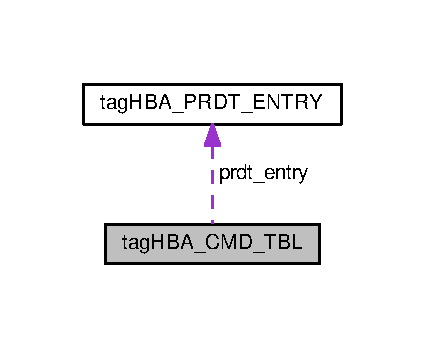
\includegraphics[width=204pt]{structtagHBA__CMD__TBL__coll__graph}
\end{center}
\end{figure}
\subsection*{Data Fields}
\begin{DoxyCompactItemize}
\item 
\hyperlink{ahci_8h_aae9749d96e15ccb4f482dd5f55d98f9b}{B\+Y\+TE} \hyperlink{structtagHBA__CMD__TBL_a3f54c56e56fb43a0c72e44f72717e53a}{cfis} \mbox{[}64\mbox{]}
\item 
\hyperlink{ahci_8h_aae9749d96e15ccb4f482dd5f55d98f9b}{B\+Y\+TE} \hyperlink{structtagHBA__CMD__TBL_a87421bf6801a2e75dd4d6e33c737857f}{acmd} \mbox{[}16\mbox{]}
\item 
\hyperlink{ahci_8h_aae9749d96e15ccb4f482dd5f55d98f9b}{B\+Y\+TE} \hyperlink{structtagHBA__CMD__TBL_a8d98e1762a624fbe9b7e510cf309046d}{rsv} \mbox{[}48\mbox{]}
\item 
\hyperlink{ahci_8h_a418c5f16923e451fc6fb5dde90dc5811}{H\+B\+A\+\_\+\+P\+R\+D\+T\+\_\+\+E\+N\+T\+RY} \hyperlink{structtagHBA__CMD__TBL_ac3a80d88e49b7bedf62d1a84217f1385}{prdt\+\_\+entry} \mbox{[}1\mbox{]}
\end{DoxyCompactItemize}


\subsection{Detailed Description}


Definition at line 477 of file ahci.\+h.



\subsection{Field Documentation}
\index{tag\+H\+B\+A\+\_\+\+C\+M\+D\+\_\+\+T\+BL@{tag\+H\+B\+A\+\_\+\+C\+M\+D\+\_\+\+T\+BL}!acmd@{acmd}}
\index{acmd@{acmd}!tag\+H\+B\+A\+\_\+\+C\+M\+D\+\_\+\+T\+BL@{tag\+H\+B\+A\+\_\+\+C\+M\+D\+\_\+\+T\+BL}}
\subsubsection[{\texorpdfstring{acmd}{acmd}}]{\setlength{\rightskip}{0pt plus 5cm}{\bf B\+Y\+TE} tag\+H\+B\+A\+\_\+\+C\+M\+D\+\_\+\+T\+B\+L\+::acmd\mbox{[}16\mbox{]}}\hypertarget{structtagHBA__CMD__TBL_a87421bf6801a2e75dd4d6e33c737857f}{}\label{structtagHBA__CMD__TBL_a87421bf6801a2e75dd4d6e33c737857f}


Definition at line 483 of file ahci.\+h.

\index{tag\+H\+B\+A\+\_\+\+C\+M\+D\+\_\+\+T\+BL@{tag\+H\+B\+A\+\_\+\+C\+M\+D\+\_\+\+T\+BL}!cfis@{cfis}}
\index{cfis@{cfis}!tag\+H\+B\+A\+\_\+\+C\+M\+D\+\_\+\+T\+BL@{tag\+H\+B\+A\+\_\+\+C\+M\+D\+\_\+\+T\+BL}}
\subsubsection[{\texorpdfstring{cfis}{cfis}}]{\setlength{\rightskip}{0pt plus 5cm}{\bf B\+Y\+TE} tag\+H\+B\+A\+\_\+\+C\+M\+D\+\_\+\+T\+B\+L\+::cfis\mbox{[}64\mbox{]}}\hypertarget{structtagHBA__CMD__TBL_a3f54c56e56fb43a0c72e44f72717e53a}{}\label{structtagHBA__CMD__TBL_a3f54c56e56fb43a0c72e44f72717e53a}


Definition at line 480 of file ahci.\+h.

\index{tag\+H\+B\+A\+\_\+\+C\+M\+D\+\_\+\+T\+BL@{tag\+H\+B\+A\+\_\+\+C\+M\+D\+\_\+\+T\+BL}!prdt\+\_\+entry@{prdt\+\_\+entry}}
\index{prdt\+\_\+entry@{prdt\+\_\+entry}!tag\+H\+B\+A\+\_\+\+C\+M\+D\+\_\+\+T\+BL@{tag\+H\+B\+A\+\_\+\+C\+M\+D\+\_\+\+T\+BL}}
\subsubsection[{\texorpdfstring{prdt\+\_\+entry}{prdt_entry}}]{\setlength{\rightskip}{0pt plus 5cm}{\bf H\+B\+A\+\_\+\+P\+R\+D\+T\+\_\+\+E\+N\+T\+RY} tag\+H\+B\+A\+\_\+\+C\+M\+D\+\_\+\+T\+B\+L\+::prdt\+\_\+entry\mbox{[}1\mbox{]}}\hypertarget{structtagHBA__CMD__TBL_ac3a80d88e49b7bedf62d1a84217f1385}{}\label{structtagHBA__CMD__TBL_ac3a80d88e49b7bedf62d1a84217f1385}


Definition at line 489 of file ahci.\+h.

\index{tag\+H\+B\+A\+\_\+\+C\+M\+D\+\_\+\+T\+BL@{tag\+H\+B\+A\+\_\+\+C\+M\+D\+\_\+\+T\+BL}!rsv@{rsv}}
\index{rsv@{rsv}!tag\+H\+B\+A\+\_\+\+C\+M\+D\+\_\+\+T\+BL@{tag\+H\+B\+A\+\_\+\+C\+M\+D\+\_\+\+T\+BL}}
\subsubsection[{\texorpdfstring{rsv}{rsv}}]{\setlength{\rightskip}{0pt plus 5cm}{\bf B\+Y\+TE} tag\+H\+B\+A\+\_\+\+C\+M\+D\+\_\+\+T\+B\+L\+::rsv\mbox{[}48\mbox{]}}\hypertarget{structtagHBA__CMD__TBL_a8d98e1762a624fbe9b7e510cf309046d}{}\label{structtagHBA__CMD__TBL_a8d98e1762a624fbe9b7e510cf309046d}


Definition at line 486 of file ahci.\+h.



The documentation for this struct was generated from the following file\+:\begin{DoxyCompactItemize}
\item 
Experimental Edition/\+Source/\+Drivers/\+A\+H\+C\+I/\hyperlink{ahci_8h}{ahci.\+h}\end{DoxyCompactItemize}

\hypertarget{structtagHBA__FIS}{}\section{tag\+H\+B\+A\+\_\+\+F\+IS Struct Reference}
\label{structtagHBA__FIS}\index{tag\+H\+B\+A\+\_\+\+F\+IS@{tag\+H\+B\+A\+\_\+\+F\+IS}}


{\ttfamily \#include $<$ahci.\+h$>$}



Collaboration diagram for tag\+H\+B\+A\+\_\+\+F\+IS\+:
\nopagebreak
\begin{figure}[H]
\begin{center}
\leavevmode
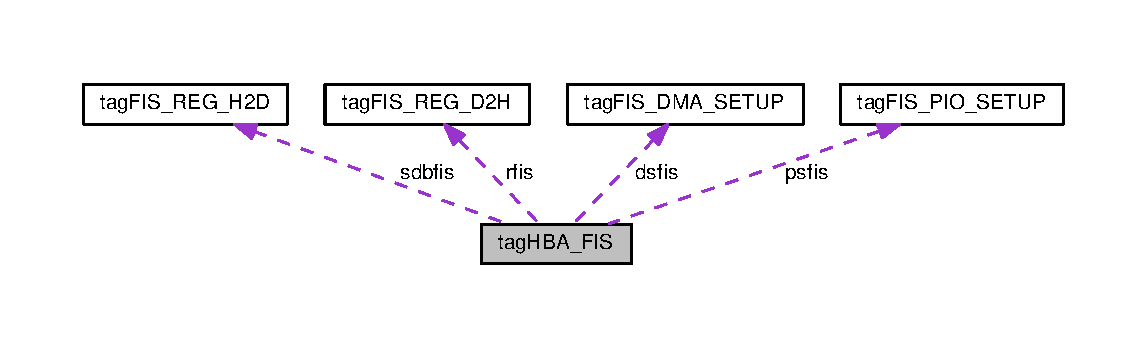
\includegraphics[width=350pt]{structtagHBA__FIS__coll__graph}
\end{center}
\end{figure}
\subsection*{Data Fields}
\begin{DoxyCompactItemize}
\item 
\hyperlink{ahci_8h_a17830d835a45fe8c22b77d388f517458}{F\+I\+S\+\_\+\+D\+M\+A\+\_\+\+S\+E\+T\+UP} \hyperlink{structtagHBA__FIS_a4a2a84ef5c00d46a159a00185e1255ca}{dsfis}
\item 
\hyperlink{ahci_8h_aae9749d96e15ccb4f482dd5f55d98f9b}{B\+Y\+TE} \hyperlink{structtagHBA__FIS_a5974d07d5e0337acef273602efead34e}{pad0} \mbox{[}4\mbox{]}
\item 
\hyperlink{ahci_8h_ad8fd7185afaad7be85168b284ce91790}{F\+I\+S\+\_\+\+P\+I\+O\+\_\+\+S\+E\+T\+UP} \hyperlink{structtagHBA__FIS_ad27f145a220089dcd16395b8a78c37b3}{psfis}
\item 
\hyperlink{ahci_8h_aae9749d96e15ccb4f482dd5f55d98f9b}{B\+Y\+TE} \hyperlink{structtagHBA__FIS_a01134a3e5ca5f0aeb05d1b087128802c}{pad1} \mbox{[}12\mbox{]}
\item 
\hyperlink{ahci_8h_a391819a2e6a838884ea809330d19c6e3}{F\+I\+S\+\_\+\+R\+E\+G\+\_\+\+D2H} \hyperlink{structtagHBA__FIS_aa67907323182bb417ef30b51616ffe19}{rfis}
\item 
\hyperlink{ahci_8h_aae9749d96e15ccb4f482dd5f55d98f9b}{B\+Y\+TE} \hyperlink{structtagHBA__FIS_ad3bd23dc216101a9fe276a0340f80ca1}{pad2} \mbox{[}4\mbox{]}
\item 
\hyperlink{ahci_8h_a8001e9b5f41caa39166f5aff6613cc3a}{F\+I\+S\+\_\+\+R\+E\+G\+\_\+\+H2D} \hyperlink{structtagHBA__FIS_a983aaa6c08cb81a58f57f4c4ca78e11a}{sdbfis}
\item 
\hyperlink{ahci_8h_aae9749d96e15ccb4f482dd5f55d98f9b}{B\+Y\+TE} \hyperlink{structtagHBA__FIS_a878d317f7fcacf4f24e7dd38567ef0a4}{ufis} \mbox{[}64\mbox{]}
\item 
\hyperlink{ahci_8h_aae9749d96e15ccb4f482dd5f55d98f9b}{B\+Y\+TE} \hyperlink{structtagHBA__FIS_a27c4d8e2aeadeca4c7dab4ff3e962f22}{rsv} \mbox{[}0x100-\/0x\+A0\mbox{]}
\end{DoxyCompactItemize}


\subsection{Detailed Description}


Definition at line 412 of file ahci.\+h.



\subsection{Field Documentation}
\index{tag\+H\+B\+A\+\_\+\+F\+IS@{tag\+H\+B\+A\+\_\+\+F\+IS}!dsfis@{dsfis}}
\index{dsfis@{dsfis}!tag\+H\+B\+A\+\_\+\+F\+IS@{tag\+H\+B\+A\+\_\+\+F\+IS}}
\subsubsection[{\texorpdfstring{dsfis}{dsfis}}]{\setlength{\rightskip}{0pt plus 5cm}{\bf F\+I\+S\+\_\+\+D\+M\+A\+\_\+\+S\+E\+T\+UP} tag\+H\+B\+A\+\_\+\+F\+I\+S\+::dsfis}\hypertarget{structtagHBA__FIS_a4a2a84ef5c00d46a159a00185e1255ca}{}\label{structtagHBA__FIS_a4a2a84ef5c00d46a159a00185e1255ca}


Definition at line 415 of file ahci.\+h.

\index{tag\+H\+B\+A\+\_\+\+F\+IS@{tag\+H\+B\+A\+\_\+\+F\+IS}!pad0@{pad0}}
\index{pad0@{pad0}!tag\+H\+B\+A\+\_\+\+F\+IS@{tag\+H\+B\+A\+\_\+\+F\+IS}}
\subsubsection[{\texorpdfstring{pad0}{pad0}}]{\setlength{\rightskip}{0pt plus 5cm}{\bf B\+Y\+TE} tag\+H\+B\+A\+\_\+\+F\+I\+S\+::pad0\mbox{[}4\mbox{]}}\hypertarget{structtagHBA__FIS_a5974d07d5e0337acef273602efead34e}{}\label{structtagHBA__FIS_a5974d07d5e0337acef273602efead34e}


Definition at line 416 of file ahci.\+h.

\index{tag\+H\+B\+A\+\_\+\+F\+IS@{tag\+H\+B\+A\+\_\+\+F\+IS}!pad1@{pad1}}
\index{pad1@{pad1}!tag\+H\+B\+A\+\_\+\+F\+IS@{tag\+H\+B\+A\+\_\+\+F\+IS}}
\subsubsection[{\texorpdfstring{pad1}{pad1}}]{\setlength{\rightskip}{0pt plus 5cm}{\bf B\+Y\+TE} tag\+H\+B\+A\+\_\+\+F\+I\+S\+::pad1\mbox{[}12\mbox{]}}\hypertarget{structtagHBA__FIS_a01134a3e5ca5f0aeb05d1b087128802c}{}\label{structtagHBA__FIS_a01134a3e5ca5f0aeb05d1b087128802c}


Definition at line 420 of file ahci.\+h.

\index{tag\+H\+B\+A\+\_\+\+F\+IS@{tag\+H\+B\+A\+\_\+\+F\+IS}!pad2@{pad2}}
\index{pad2@{pad2}!tag\+H\+B\+A\+\_\+\+F\+IS@{tag\+H\+B\+A\+\_\+\+F\+IS}}
\subsubsection[{\texorpdfstring{pad2}{pad2}}]{\setlength{\rightskip}{0pt plus 5cm}{\bf B\+Y\+TE} tag\+H\+B\+A\+\_\+\+F\+I\+S\+::pad2\mbox{[}4\mbox{]}}\hypertarget{structtagHBA__FIS_ad3bd23dc216101a9fe276a0340f80ca1}{}\label{structtagHBA__FIS_ad3bd23dc216101a9fe276a0340f80ca1}


Definition at line 424 of file ahci.\+h.

\index{tag\+H\+B\+A\+\_\+\+F\+IS@{tag\+H\+B\+A\+\_\+\+F\+IS}!psfis@{psfis}}
\index{psfis@{psfis}!tag\+H\+B\+A\+\_\+\+F\+IS@{tag\+H\+B\+A\+\_\+\+F\+IS}}
\subsubsection[{\texorpdfstring{psfis}{psfis}}]{\setlength{\rightskip}{0pt plus 5cm}{\bf F\+I\+S\+\_\+\+P\+I\+O\+\_\+\+S\+E\+T\+UP} tag\+H\+B\+A\+\_\+\+F\+I\+S\+::psfis}\hypertarget{structtagHBA__FIS_ad27f145a220089dcd16395b8a78c37b3}{}\label{structtagHBA__FIS_ad27f145a220089dcd16395b8a78c37b3}


Definition at line 419 of file ahci.\+h.

\index{tag\+H\+B\+A\+\_\+\+F\+IS@{tag\+H\+B\+A\+\_\+\+F\+IS}!rfis@{rfis}}
\index{rfis@{rfis}!tag\+H\+B\+A\+\_\+\+F\+IS@{tag\+H\+B\+A\+\_\+\+F\+IS}}
\subsubsection[{\texorpdfstring{rfis}{rfis}}]{\setlength{\rightskip}{0pt plus 5cm}{\bf F\+I\+S\+\_\+\+R\+E\+G\+\_\+\+D2H} tag\+H\+B\+A\+\_\+\+F\+I\+S\+::rfis}\hypertarget{structtagHBA__FIS_aa67907323182bb417ef30b51616ffe19}{}\label{structtagHBA__FIS_aa67907323182bb417ef30b51616ffe19}


Definition at line 423 of file ahci.\+h.

\index{tag\+H\+B\+A\+\_\+\+F\+IS@{tag\+H\+B\+A\+\_\+\+F\+IS}!rsv@{rsv}}
\index{rsv@{rsv}!tag\+H\+B\+A\+\_\+\+F\+IS@{tag\+H\+B\+A\+\_\+\+F\+IS}}
\subsubsection[{\texorpdfstring{rsv}{rsv}}]{\setlength{\rightskip}{0pt plus 5cm}{\bf B\+Y\+TE} tag\+H\+B\+A\+\_\+\+F\+I\+S\+::rsv\mbox{[}0x100-\/0x\+A0\mbox{]}}\hypertarget{structtagHBA__FIS_a27c4d8e2aeadeca4c7dab4ff3e962f22}{}\label{structtagHBA__FIS_a27c4d8e2aeadeca4c7dab4ff3e962f22}


Definition at line 433 of file ahci.\+h.

\index{tag\+H\+B\+A\+\_\+\+F\+IS@{tag\+H\+B\+A\+\_\+\+F\+IS}!sdbfis@{sdbfis}}
\index{sdbfis@{sdbfis}!tag\+H\+B\+A\+\_\+\+F\+IS@{tag\+H\+B\+A\+\_\+\+F\+IS}}
\subsubsection[{\texorpdfstring{sdbfis}{sdbfis}}]{\setlength{\rightskip}{0pt plus 5cm}{\bf F\+I\+S\+\_\+\+R\+E\+G\+\_\+\+H2D} tag\+H\+B\+A\+\_\+\+F\+I\+S\+::sdbfis}\hypertarget{structtagHBA__FIS_a983aaa6c08cb81a58f57f4c4ca78e11a}{}\label{structtagHBA__FIS_a983aaa6c08cb81a58f57f4c4ca78e11a}


Definition at line 427 of file ahci.\+h.

\index{tag\+H\+B\+A\+\_\+\+F\+IS@{tag\+H\+B\+A\+\_\+\+F\+IS}!ufis@{ufis}}
\index{ufis@{ufis}!tag\+H\+B\+A\+\_\+\+F\+IS@{tag\+H\+B\+A\+\_\+\+F\+IS}}
\subsubsection[{\texorpdfstring{ufis}{ufis}}]{\setlength{\rightskip}{0pt plus 5cm}{\bf B\+Y\+TE} tag\+H\+B\+A\+\_\+\+F\+I\+S\+::ufis\mbox{[}64\mbox{]}}\hypertarget{structtagHBA__FIS_a878d317f7fcacf4f24e7dd38567ef0a4}{}\label{structtagHBA__FIS_a878d317f7fcacf4f24e7dd38567ef0a4}


Definition at line 430 of file ahci.\+h.



The documentation for this struct was generated from the following file\+:\begin{DoxyCompactItemize}
\item 
Experimental Edition/\+Source/\+Drivers/\+A\+H\+C\+I/\hyperlink{ahci_8h}{ahci.\+h}\end{DoxyCompactItemize}

\hypertarget{structtagHBA__MEM}{}\section{tag\+H\+B\+A\+\_\+\+M\+EM Struct Reference}
\label{structtagHBA__MEM}\index{tag\+H\+B\+A\+\_\+\+M\+EM@{tag\+H\+B\+A\+\_\+\+M\+EM}}


{\ttfamily \#include $<$ahci.\+h$>$}



Collaboration diagram for tag\+H\+B\+A\+\_\+\+M\+EM\+:
\nopagebreak
\begin{figure}[H]
\begin{center}
\leavevmode
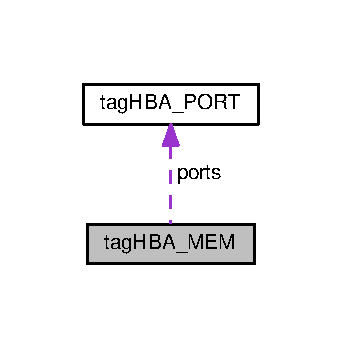
\includegraphics[width=164pt]{structtagHBA__MEM__coll__graph}
\end{center}
\end{figure}
\subsection*{Data Fields}
\begin{DoxyCompactItemize}
\item 
\hyperlink{ahci_8h_af483253b2143078cede883fc3c111ad2}{D\+W\+O\+RD} \hyperlink{structtagHBA__MEM_ade2b27aa0751affb0a2a3ae4524dad1d}{cap}
\item 
\hyperlink{ahci_8h_af483253b2143078cede883fc3c111ad2}{D\+W\+O\+RD} \hyperlink{structtagHBA__MEM_aa17d9a745823a5271d26b37dc7961806}{ghc}
\item 
\hyperlink{ahci_8h_af483253b2143078cede883fc3c111ad2}{D\+W\+O\+RD} \hyperlink{structtagHBA__MEM_aa77427e1a0606dcb6751929b7202d0e5}{is}
\item 
\hyperlink{ahci_8h_af483253b2143078cede883fc3c111ad2}{D\+W\+O\+RD} \hyperlink{structtagHBA__MEM_ab16699350ab40792061df91f7bf7fe3e}{pi}
\item 
\hyperlink{ahci_8h_af483253b2143078cede883fc3c111ad2}{D\+W\+O\+RD} \hyperlink{structtagHBA__MEM_a733df04d8b6b74306fae06a578524c4b}{vs}
\item 
\hyperlink{ahci_8h_af483253b2143078cede883fc3c111ad2}{D\+W\+O\+RD} \hyperlink{structtagHBA__MEM_ac0d65e18ffe93d59049bcd31cac005c2}{ccc\+\_\+ctl}
\item 
\hyperlink{ahci_8h_af483253b2143078cede883fc3c111ad2}{D\+W\+O\+RD} \hyperlink{structtagHBA__MEM_a21a5848ae6eb662f4b198b2f3715d1bc}{ccc\+\_\+pts}
\item 
\hyperlink{ahci_8h_af483253b2143078cede883fc3c111ad2}{D\+W\+O\+RD} \hyperlink{structtagHBA__MEM_aec82a290be8762fbfb6094763606d977}{em\+\_\+loc}
\item 
\hyperlink{ahci_8h_af483253b2143078cede883fc3c111ad2}{D\+W\+O\+RD} \hyperlink{structtagHBA__MEM_ae6b55e0ca53cd0cdc641aae9dff0aa4d}{em\+\_\+ctl}
\item 
\hyperlink{ahci_8h_af483253b2143078cede883fc3c111ad2}{D\+W\+O\+RD} \hyperlink{structtagHBA__MEM_a54e8a62903ba72eb3a6cf3bae97da878}{cap2}
\item 
\hyperlink{ahci_8h_af483253b2143078cede883fc3c111ad2}{D\+W\+O\+RD} \hyperlink{structtagHBA__MEM_a1efc56b8a33d024424d582d4f5d20c76}{bohc}
\item 
\hyperlink{ahci_8h_aae9749d96e15ccb4f482dd5f55d98f9b}{B\+Y\+TE} \hyperlink{structtagHBA__MEM_ad2e9bac8871df4331a830a4f3869affa}{rsv} \mbox{[}0x\+A0-\/0x2\+C\mbox{]}
\item 
\hyperlink{ahci_8h_aae9749d96e15ccb4f482dd5f55d98f9b}{B\+Y\+TE} \hyperlink{structtagHBA__MEM_a3869422a65c7777a6f5e013df134cf8a}{vendor} \mbox{[}0x100-\/0x\+A0\mbox{]}
\item 
\hyperlink{ahci_8h_ace0b5fb17e1a588ab172cbf436c0a3d3}{H\+B\+A\+\_\+\+P\+O\+RT} \hyperlink{structtagHBA__MEM_a4228a9fb80ba497724bda96cfe288c1d}{ports} \mbox{[}32\mbox{]}
\end{DoxyCompactItemize}


\subsection{Detailed Description}


Definition at line 387 of file ahci.\+h.



\subsection{Field Documentation}
\index{tag\+H\+B\+A\+\_\+\+M\+EM@{tag\+H\+B\+A\+\_\+\+M\+EM}!bohc@{bohc}}
\index{bohc@{bohc}!tag\+H\+B\+A\+\_\+\+M\+EM@{tag\+H\+B\+A\+\_\+\+M\+EM}}
\subsubsection[{\texorpdfstring{bohc}{bohc}}]{\setlength{\rightskip}{0pt plus 5cm}{\bf D\+W\+O\+RD} tag\+H\+B\+A\+\_\+\+M\+E\+M\+::bohc}\hypertarget{structtagHBA__MEM_a1efc56b8a33d024424d582d4f5d20c76}{}\label{structtagHBA__MEM_a1efc56b8a33d024424d582d4f5d20c76}


Definition at line 400 of file ahci.\+h.

\index{tag\+H\+B\+A\+\_\+\+M\+EM@{tag\+H\+B\+A\+\_\+\+M\+EM}!cap@{cap}}
\index{cap@{cap}!tag\+H\+B\+A\+\_\+\+M\+EM@{tag\+H\+B\+A\+\_\+\+M\+EM}}
\subsubsection[{\texorpdfstring{cap}{cap}}]{\setlength{\rightskip}{0pt plus 5cm}{\bf D\+W\+O\+RD} tag\+H\+B\+A\+\_\+\+M\+E\+M\+::cap}\hypertarget{structtagHBA__MEM_ade2b27aa0751affb0a2a3ae4524dad1d}{}\label{structtagHBA__MEM_ade2b27aa0751affb0a2a3ae4524dad1d}


Definition at line 390 of file ahci.\+h.

\index{tag\+H\+B\+A\+\_\+\+M\+EM@{tag\+H\+B\+A\+\_\+\+M\+EM}!cap2@{cap2}}
\index{cap2@{cap2}!tag\+H\+B\+A\+\_\+\+M\+EM@{tag\+H\+B\+A\+\_\+\+M\+EM}}
\subsubsection[{\texorpdfstring{cap2}{cap2}}]{\setlength{\rightskip}{0pt plus 5cm}{\bf D\+W\+O\+RD} tag\+H\+B\+A\+\_\+\+M\+E\+M\+::cap2}\hypertarget{structtagHBA__MEM_a54e8a62903ba72eb3a6cf3bae97da878}{}\label{structtagHBA__MEM_a54e8a62903ba72eb3a6cf3bae97da878}


Definition at line 399 of file ahci.\+h.

\index{tag\+H\+B\+A\+\_\+\+M\+EM@{tag\+H\+B\+A\+\_\+\+M\+EM}!ccc\+\_\+ctl@{ccc\+\_\+ctl}}
\index{ccc\+\_\+ctl@{ccc\+\_\+ctl}!tag\+H\+B\+A\+\_\+\+M\+EM@{tag\+H\+B\+A\+\_\+\+M\+EM}}
\subsubsection[{\texorpdfstring{ccc\+\_\+ctl}{ccc_ctl}}]{\setlength{\rightskip}{0pt plus 5cm}{\bf D\+W\+O\+RD} tag\+H\+B\+A\+\_\+\+M\+E\+M\+::ccc\+\_\+ctl}\hypertarget{structtagHBA__MEM_ac0d65e18ffe93d59049bcd31cac005c2}{}\label{structtagHBA__MEM_ac0d65e18ffe93d59049bcd31cac005c2}


Definition at line 395 of file ahci.\+h.

\index{tag\+H\+B\+A\+\_\+\+M\+EM@{tag\+H\+B\+A\+\_\+\+M\+EM}!ccc\+\_\+pts@{ccc\+\_\+pts}}
\index{ccc\+\_\+pts@{ccc\+\_\+pts}!tag\+H\+B\+A\+\_\+\+M\+EM@{tag\+H\+B\+A\+\_\+\+M\+EM}}
\subsubsection[{\texorpdfstring{ccc\+\_\+pts}{ccc_pts}}]{\setlength{\rightskip}{0pt plus 5cm}{\bf D\+W\+O\+RD} tag\+H\+B\+A\+\_\+\+M\+E\+M\+::ccc\+\_\+pts}\hypertarget{structtagHBA__MEM_a21a5848ae6eb662f4b198b2f3715d1bc}{}\label{structtagHBA__MEM_a21a5848ae6eb662f4b198b2f3715d1bc}


Definition at line 396 of file ahci.\+h.

\index{tag\+H\+B\+A\+\_\+\+M\+EM@{tag\+H\+B\+A\+\_\+\+M\+EM}!em\+\_\+ctl@{em\+\_\+ctl}}
\index{em\+\_\+ctl@{em\+\_\+ctl}!tag\+H\+B\+A\+\_\+\+M\+EM@{tag\+H\+B\+A\+\_\+\+M\+EM}}
\subsubsection[{\texorpdfstring{em\+\_\+ctl}{em_ctl}}]{\setlength{\rightskip}{0pt plus 5cm}{\bf D\+W\+O\+RD} tag\+H\+B\+A\+\_\+\+M\+E\+M\+::em\+\_\+ctl}\hypertarget{structtagHBA__MEM_ae6b55e0ca53cd0cdc641aae9dff0aa4d}{}\label{structtagHBA__MEM_ae6b55e0ca53cd0cdc641aae9dff0aa4d}


Definition at line 398 of file ahci.\+h.

\index{tag\+H\+B\+A\+\_\+\+M\+EM@{tag\+H\+B\+A\+\_\+\+M\+EM}!em\+\_\+loc@{em\+\_\+loc}}
\index{em\+\_\+loc@{em\+\_\+loc}!tag\+H\+B\+A\+\_\+\+M\+EM@{tag\+H\+B\+A\+\_\+\+M\+EM}}
\subsubsection[{\texorpdfstring{em\+\_\+loc}{em_loc}}]{\setlength{\rightskip}{0pt plus 5cm}{\bf D\+W\+O\+RD} tag\+H\+B\+A\+\_\+\+M\+E\+M\+::em\+\_\+loc}\hypertarget{structtagHBA__MEM_aec82a290be8762fbfb6094763606d977}{}\label{structtagHBA__MEM_aec82a290be8762fbfb6094763606d977}


Definition at line 397 of file ahci.\+h.

\index{tag\+H\+B\+A\+\_\+\+M\+EM@{tag\+H\+B\+A\+\_\+\+M\+EM}!ghc@{ghc}}
\index{ghc@{ghc}!tag\+H\+B\+A\+\_\+\+M\+EM@{tag\+H\+B\+A\+\_\+\+M\+EM}}
\subsubsection[{\texorpdfstring{ghc}{ghc}}]{\setlength{\rightskip}{0pt plus 5cm}{\bf D\+W\+O\+RD} tag\+H\+B\+A\+\_\+\+M\+E\+M\+::ghc}\hypertarget{structtagHBA__MEM_aa17d9a745823a5271d26b37dc7961806}{}\label{structtagHBA__MEM_aa17d9a745823a5271d26b37dc7961806}


Definition at line 391 of file ahci.\+h.

\index{tag\+H\+B\+A\+\_\+\+M\+EM@{tag\+H\+B\+A\+\_\+\+M\+EM}!is@{is}}
\index{is@{is}!tag\+H\+B\+A\+\_\+\+M\+EM@{tag\+H\+B\+A\+\_\+\+M\+EM}}
\subsubsection[{\texorpdfstring{is}{is}}]{\setlength{\rightskip}{0pt plus 5cm}{\bf D\+W\+O\+RD} tag\+H\+B\+A\+\_\+\+M\+E\+M\+::is}\hypertarget{structtagHBA__MEM_aa77427e1a0606dcb6751929b7202d0e5}{}\label{structtagHBA__MEM_aa77427e1a0606dcb6751929b7202d0e5}


Definition at line 392 of file ahci.\+h.

\index{tag\+H\+B\+A\+\_\+\+M\+EM@{tag\+H\+B\+A\+\_\+\+M\+EM}!pi@{pi}}
\index{pi@{pi}!tag\+H\+B\+A\+\_\+\+M\+EM@{tag\+H\+B\+A\+\_\+\+M\+EM}}
\subsubsection[{\texorpdfstring{pi}{pi}}]{\setlength{\rightskip}{0pt plus 5cm}{\bf D\+W\+O\+RD} tag\+H\+B\+A\+\_\+\+M\+E\+M\+::pi}\hypertarget{structtagHBA__MEM_ab16699350ab40792061df91f7bf7fe3e}{}\label{structtagHBA__MEM_ab16699350ab40792061df91f7bf7fe3e}


Definition at line 393 of file ahci.\+h.

\index{tag\+H\+B\+A\+\_\+\+M\+EM@{tag\+H\+B\+A\+\_\+\+M\+EM}!ports@{ports}}
\index{ports@{ports}!tag\+H\+B\+A\+\_\+\+M\+EM@{tag\+H\+B\+A\+\_\+\+M\+EM}}
\subsubsection[{\texorpdfstring{ports}{ports}}]{\setlength{\rightskip}{0pt plus 5cm}{\bf H\+B\+A\+\_\+\+P\+O\+RT} tag\+H\+B\+A\+\_\+\+M\+E\+M\+::ports\mbox{[}32\mbox{]}}\hypertarget{structtagHBA__MEM_a4228a9fb80ba497724bda96cfe288c1d}{}\label{structtagHBA__MEM_a4228a9fb80ba497724bda96cfe288c1d}


Definition at line 409 of file ahci.\+h.

\index{tag\+H\+B\+A\+\_\+\+M\+EM@{tag\+H\+B\+A\+\_\+\+M\+EM}!rsv@{rsv}}
\index{rsv@{rsv}!tag\+H\+B\+A\+\_\+\+M\+EM@{tag\+H\+B\+A\+\_\+\+M\+EM}}
\subsubsection[{\texorpdfstring{rsv}{rsv}}]{\setlength{\rightskip}{0pt plus 5cm}{\bf B\+Y\+TE} tag\+H\+B\+A\+\_\+\+M\+E\+M\+::rsv\mbox{[}0x\+A0-\/0x2\+C\mbox{]}}\hypertarget{structtagHBA__MEM_ad2e9bac8871df4331a830a4f3869affa}{}\label{structtagHBA__MEM_ad2e9bac8871df4331a830a4f3869affa}


Definition at line 403 of file ahci.\+h.

\index{tag\+H\+B\+A\+\_\+\+M\+EM@{tag\+H\+B\+A\+\_\+\+M\+EM}!vendor@{vendor}}
\index{vendor@{vendor}!tag\+H\+B\+A\+\_\+\+M\+EM@{tag\+H\+B\+A\+\_\+\+M\+EM}}
\subsubsection[{\texorpdfstring{vendor}{vendor}}]{\setlength{\rightskip}{0pt plus 5cm}{\bf B\+Y\+TE} tag\+H\+B\+A\+\_\+\+M\+E\+M\+::vendor\mbox{[}0x100-\/0x\+A0\mbox{]}}\hypertarget{structtagHBA__MEM_a3869422a65c7777a6f5e013df134cf8a}{}\label{structtagHBA__MEM_a3869422a65c7777a6f5e013df134cf8a}


Definition at line 406 of file ahci.\+h.

\index{tag\+H\+B\+A\+\_\+\+M\+EM@{tag\+H\+B\+A\+\_\+\+M\+EM}!vs@{vs}}
\index{vs@{vs}!tag\+H\+B\+A\+\_\+\+M\+EM@{tag\+H\+B\+A\+\_\+\+M\+EM}}
\subsubsection[{\texorpdfstring{vs}{vs}}]{\setlength{\rightskip}{0pt plus 5cm}{\bf D\+W\+O\+RD} tag\+H\+B\+A\+\_\+\+M\+E\+M\+::vs}\hypertarget{structtagHBA__MEM_a733df04d8b6b74306fae06a578524c4b}{}\label{structtagHBA__MEM_a733df04d8b6b74306fae06a578524c4b}


Definition at line 394 of file ahci.\+h.



The documentation for this struct was generated from the following file\+:\begin{DoxyCompactItemize}
\item 
Experimental Edition/\+Source/\+Drivers/\+A\+H\+C\+I/\hyperlink{ahci_8h}{ahci.\+h}\end{DoxyCompactItemize}

\hypertarget{structtagHBA__PORT}{}\section{tag\+H\+B\+A\+\_\+\+P\+O\+RT Struct Reference}
\label{structtagHBA__PORT}\index{tag\+H\+B\+A\+\_\+\+P\+O\+RT@{tag\+H\+B\+A\+\_\+\+P\+O\+RT}}


{\ttfamily \#include $<$ahci.\+h$>$}

\subsection*{Data Fields}
\begin{DoxyCompactItemize}
\item 
\hyperlink{ahci_8h_af483253b2143078cede883fc3c111ad2}{D\+W\+O\+RD} \hyperlink{structtagHBA__PORT_a780c8e115f777212d1c07e40635688bd}{clb}
\item 
\hyperlink{ahci_8h_af483253b2143078cede883fc3c111ad2}{D\+W\+O\+RD} \hyperlink{structtagHBA__PORT_a1035c66916eb3226c0fb5c81162a37b3}{clbu}
\item 
\hyperlink{ahci_8h_af483253b2143078cede883fc3c111ad2}{D\+W\+O\+RD} \hyperlink{structtagHBA__PORT_a79e614d89d9277d1da8c1746fecdd0ca}{fb}
\item 
\hyperlink{ahci_8h_af483253b2143078cede883fc3c111ad2}{D\+W\+O\+RD} \hyperlink{structtagHBA__PORT_accb4b0268c93dbd575a4927c528114a2}{fbu}
\item 
\hyperlink{ahci_8h_af483253b2143078cede883fc3c111ad2}{D\+W\+O\+RD} \hyperlink{structtagHBA__PORT_a8580d4658e46190fc8db40a6b298bde7}{is}
\item 
\hyperlink{ahci_8h_af483253b2143078cede883fc3c111ad2}{D\+W\+O\+RD} \hyperlink{structtagHBA__PORT_a6a5c3ee42874ffed476d7ba542b7b84d}{ie}
\item 
\hyperlink{ahci_8h_af483253b2143078cede883fc3c111ad2}{D\+W\+O\+RD} \hyperlink{structtagHBA__PORT_a95c7a739718780e85a8c7c40fdf14d3b}{cmd}
\item 
\hyperlink{ahci_8h_af483253b2143078cede883fc3c111ad2}{D\+W\+O\+RD} \hyperlink{structtagHBA__PORT_a93acfc284634754a95549854ede8c63c}{rsv0}
\item 
\hyperlink{ahci_8h_af483253b2143078cede883fc3c111ad2}{D\+W\+O\+RD} \hyperlink{structtagHBA__PORT_aa37d7e6ddbbcf7bf9122a6749f90bda9}{tfd}
\item 
\hyperlink{ahci_8h_af483253b2143078cede883fc3c111ad2}{D\+W\+O\+RD} \hyperlink{structtagHBA__PORT_a8da0417fcedbffa65a307f3d11c4f536}{sig}
\item 
\hyperlink{ahci_8h_af483253b2143078cede883fc3c111ad2}{D\+W\+O\+RD} \hyperlink{structtagHBA__PORT_ad96e7508ddfd2c65f76bc866b24bd2fd}{ssts}
\item 
\hyperlink{ahci_8h_af483253b2143078cede883fc3c111ad2}{D\+W\+O\+RD} \hyperlink{structtagHBA__PORT_af3a750481870d182c0a3b8d50f0fd407}{sctl}
\item 
\hyperlink{ahci_8h_af483253b2143078cede883fc3c111ad2}{D\+W\+O\+RD} \hyperlink{structtagHBA__PORT_a3dffc0b938071d117344f0af99daf43c}{serr}
\item 
\hyperlink{ahci_8h_af483253b2143078cede883fc3c111ad2}{D\+W\+O\+RD} \hyperlink{structtagHBA__PORT_a9e82a6b395a7d847987303bd711239e7}{sact}
\item 
\hyperlink{ahci_8h_af483253b2143078cede883fc3c111ad2}{D\+W\+O\+RD} \hyperlink{structtagHBA__PORT_a908838f0c781ae69d7bef4074e2e7d2f}{ci}
\item 
\hyperlink{ahci_8h_af483253b2143078cede883fc3c111ad2}{D\+W\+O\+RD} \hyperlink{structtagHBA__PORT_a21ca4c8f43026c753673b47d6c89b022}{sntf}
\item 
\hyperlink{ahci_8h_af483253b2143078cede883fc3c111ad2}{D\+W\+O\+RD} \hyperlink{structtagHBA__PORT_a230076311b6afef9af139b3ca7cec13a}{fbs}
\item 
\hyperlink{ahci_8h_af483253b2143078cede883fc3c111ad2}{D\+W\+O\+RD} \hyperlink{structtagHBA__PORT_aadacc981aa847f84f0443d883fc15931}{rsv1} \mbox{[}11\mbox{]}
\item 
\hyperlink{ahci_8h_af483253b2143078cede883fc3c111ad2}{D\+W\+O\+RD} \hyperlink{structtagHBA__PORT_a8d00362b7a8c6f595c99f6eb87bededf}{vendor} \mbox{[}4\mbox{]}
\end{DoxyCompactItemize}


\subsection{Detailed Description}


Definition at line 364 of file ahci.\+h.



\subsection{Field Documentation}
\index{tag\+H\+B\+A\+\_\+\+P\+O\+RT@{tag\+H\+B\+A\+\_\+\+P\+O\+RT}!ci@{ci}}
\index{ci@{ci}!tag\+H\+B\+A\+\_\+\+P\+O\+RT@{tag\+H\+B\+A\+\_\+\+P\+O\+RT}}
\subsubsection[{\texorpdfstring{ci}{ci}}]{\setlength{\rightskip}{0pt plus 5cm}{\bf D\+W\+O\+RD} tag\+H\+B\+A\+\_\+\+P\+O\+R\+T\+::ci}\hypertarget{structtagHBA__PORT_a908838f0c781ae69d7bef4074e2e7d2f}{}\label{structtagHBA__PORT_a908838f0c781ae69d7bef4074e2e7d2f}


Definition at line 380 of file ahci.\+h.

\index{tag\+H\+B\+A\+\_\+\+P\+O\+RT@{tag\+H\+B\+A\+\_\+\+P\+O\+RT}!clb@{clb}}
\index{clb@{clb}!tag\+H\+B\+A\+\_\+\+P\+O\+RT@{tag\+H\+B\+A\+\_\+\+P\+O\+RT}}
\subsubsection[{\texorpdfstring{clb}{clb}}]{\setlength{\rightskip}{0pt plus 5cm}{\bf D\+W\+O\+RD} tag\+H\+B\+A\+\_\+\+P\+O\+R\+T\+::clb}\hypertarget{structtagHBA__PORT_a780c8e115f777212d1c07e40635688bd}{}\label{structtagHBA__PORT_a780c8e115f777212d1c07e40635688bd}


Definition at line 366 of file ahci.\+h.

\index{tag\+H\+B\+A\+\_\+\+P\+O\+RT@{tag\+H\+B\+A\+\_\+\+P\+O\+RT}!clbu@{clbu}}
\index{clbu@{clbu}!tag\+H\+B\+A\+\_\+\+P\+O\+RT@{tag\+H\+B\+A\+\_\+\+P\+O\+RT}}
\subsubsection[{\texorpdfstring{clbu}{clbu}}]{\setlength{\rightskip}{0pt plus 5cm}{\bf D\+W\+O\+RD} tag\+H\+B\+A\+\_\+\+P\+O\+R\+T\+::clbu}\hypertarget{structtagHBA__PORT_a1035c66916eb3226c0fb5c81162a37b3}{}\label{structtagHBA__PORT_a1035c66916eb3226c0fb5c81162a37b3}


Definition at line 367 of file ahci.\+h.

\index{tag\+H\+B\+A\+\_\+\+P\+O\+RT@{tag\+H\+B\+A\+\_\+\+P\+O\+RT}!cmd@{cmd}}
\index{cmd@{cmd}!tag\+H\+B\+A\+\_\+\+P\+O\+RT@{tag\+H\+B\+A\+\_\+\+P\+O\+RT}}
\subsubsection[{\texorpdfstring{cmd}{cmd}}]{\setlength{\rightskip}{0pt plus 5cm}{\bf D\+W\+O\+RD} tag\+H\+B\+A\+\_\+\+P\+O\+R\+T\+::cmd}\hypertarget{structtagHBA__PORT_a95c7a739718780e85a8c7c40fdf14d3b}{}\label{structtagHBA__PORT_a95c7a739718780e85a8c7c40fdf14d3b}


Definition at line 372 of file ahci.\+h.

\index{tag\+H\+B\+A\+\_\+\+P\+O\+RT@{tag\+H\+B\+A\+\_\+\+P\+O\+RT}!fb@{fb}}
\index{fb@{fb}!tag\+H\+B\+A\+\_\+\+P\+O\+RT@{tag\+H\+B\+A\+\_\+\+P\+O\+RT}}
\subsubsection[{\texorpdfstring{fb}{fb}}]{\setlength{\rightskip}{0pt plus 5cm}{\bf D\+W\+O\+RD} tag\+H\+B\+A\+\_\+\+P\+O\+R\+T\+::fb}\hypertarget{structtagHBA__PORT_a79e614d89d9277d1da8c1746fecdd0ca}{}\label{structtagHBA__PORT_a79e614d89d9277d1da8c1746fecdd0ca}


Definition at line 368 of file ahci.\+h.

\index{tag\+H\+B\+A\+\_\+\+P\+O\+RT@{tag\+H\+B\+A\+\_\+\+P\+O\+RT}!fbs@{fbs}}
\index{fbs@{fbs}!tag\+H\+B\+A\+\_\+\+P\+O\+RT@{tag\+H\+B\+A\+\_\+\+P\+O\+RT}}
\subsubsection[{\texorpdfstring{fbs}{fbs}}]{\setlength{\rightskip}{0pt plus 5cm}{\bf D\+W\+O\+RD} tag\+H\+B\+A\+\_\+\+P\+O\+R\+T\+::fbs}\hypertarget{structtagHBA__PORT_a230076311b6afef9af139b3ca7cec13a}{}\label{structtagHBA__PORT_a230076311b6afef9af139b3ca7cec13a}


Definition at line 382 of file ahci.\+h.

\index{tag\+H\+B\+A\+\_\+\+P\+O\+RT@{tag\+H\+B\+A\+\_\+\+P\+O\+RT}!fbu@{fbu}}
\index{fbu@{fbu}!tag\+H\+B\+A\+\_\+\+P\+O\+RT@{tag\+H\+B\+A\+\_\+\+P\+O\+RT}}
\subsubsection[{\texorpdfstring{fbu}{fbu}}]{\setlength{\rightskip}{0pt plus 5cm}{\bf D\+W\+O\+RD} tag\+H\+B\+A\+\_\+\+P\+O\+R\+T\+::fbu}\hypertarget{structtagHBA__PORT_accb4b0268c93dbd575a4927c528114a2}{}\label{structtagHBA__PORT_accb4b0268c93dbd575a4927c528114a2}


Definition at line 369 of file ahci.\+h.

\index{tag\+H\+B\+A\+\_\+\+P\+O\+RT@{tag\+H\+B\+A\+\_\+\+P\+O\+RT}!ie@{ie}}
\index{ie@{ie}!tag\+H\+B\+A\+\_\+\+P\+O\+RT@{tag\+H\+B\+A\+\_\+\+P\+O\+RT}}
\subsubsection[{\texorpdfstring{ie}{ie}}]{\setlength{\rightskip}{0pt plus 5cm}{\bf D\+W\+O\+RD} tag\+H\+B\+A\+\_\+\+P\+O\+R\+T\+::ie}\hypertarget{structtagHBA__PORT_a6a5c3ee42874ffed476d7ba542b7b84d}{}\label{structtagHBA__PORT_a6a5c3ee42874ffed476d7ba542b7b84d}


Definition at line 371 of file ahci.\+h.

\index{tag\+H\+B\+A\+\_\+\+P\+O\+RT@{tag\+H\+B\+A\+\_\+\+P\+O\+RT}!is@{is}}
\index{is@{is}!tag\+H\+B\+A\+\_\+\+P\+O\+RT@{tag\+H\+B\+A\+\_\+\+P\+O\+RT}}
\subsubsection[{\texorpdfstring{is}{is}}]{\setlength{\rightskip}{0pt plus 5cm}{\bf D\+W\+O\+RD} tag\+H\+B\+A\+\_\+\+P\+O\+R\+T\+::is}\hypertarget{structtagHBA__PORT_a8580d4658e46190fc8db40a6b298bde7}{}\label{structtagHBA__PORT_a8580d4658e46190fc8db40a6b298bde7}


Definition at line 370 of file ahci.\+h.

\index{tag\+H\+B\+A\+\_\+\+P\+O\+RT@{tag\+H\+B\+A\+\_\+\+P\+O\+RT}!rsv0@{rsv0}}
\index{rsv0@{rsv0}!tag\+H\+B\+A\+\_\+\+P\+O\+RT@{tag\+H\+B\+A\+\_\+\+P\+O\+RT}}
\subsubsection[{\texorpdfstring{rsv0}{rsv0}}]{\setlength{\rightskip}{0pt plus 5cm}{\bf D\+W\+O\+RD} tag\+H\+B\+A\+\_\+\+P\+O\+R\+T\+::rsv0}\hypertarget{structtagHBA__PORT_a93acfc284634754a95549854ede8c63c}{}\label{structtagHBA__PORT_a93acfc284634754a95549854ede8c63c}


Definition at line 373 of file ahci.\+h.

\index{tag\+H\+B\+A\+\_\+\+P\+O\+RT@{tag\+H\+B\+A\+\_\+\+P\+O\+RT}!rsv1@{rsv1}}
\index{rsv1@{rsv1}!tag\+H\+B\+A\+\_\+\+P\+O\+RT@{tag\+H\+B\+A\+\_\+\+P\+O\+RT}}
\subsubsection[{\texorpdfstring{rsv1}{rsv1}}]{\setlength{\rightskip}{0pt plus 5cm}{\bf D\+W\+O\+RD} tag\+H\+B\+A\+\_\+\+P\+O\+R\+T\+::rsv1\mbox{[}11\mbox{]}}\hypertarget{structtagHBA__PORT_aadacc981aa847f84f0443d883fc15931}{}\label{structtagHBA__PORT_aadacc981aa847f84f0443d883fc15931}


Definition at line 383 of file ahci.\+h.

\index{tag\+H\+B\+A\+\_\+\+P\+O\+RT@{tag\+H\+B\+A\+\_\+\+P\+O\+RT}!sact@{sact}}
\index{sact@{sact}!tag\+H\+B\+A\+\_\+\+P\+O\+RT@{tag\+H\+B\+A\+\_\+\+P\+O\+RT}}
\subsubsection[{\texorpdfstring{sact}{sact}}]{\setlength{\rightskip}{0pt plus 5cm}{\bf D\+W\+O\+RD} tag\+H\+B\+A\+\_\+\+P\+O\+R\+T\+::sact}\hypertarget{structtagHBA__PORT_a9e82a6b395a7d847987303bd711239e7}{}\label{structtagHBA__PORT_a9e82a6b395a7d847987303bd711239e7}


Definition at line 379 of file ahci.\+h.

\index{tag\+H\+B\+A\+\_\+\+P\+O\+RT@{tag\+H\+B\+A\+\_\+\+P\+O\+RT}!sctl@{sctl}}
\index{sctl@{sctl}!tag\+H\+B\+A\+\_\+\+P\+O\+RT@{tag\+H\+B\+A\+\_\+\+P\+O\+RT}}
\subsubsection[{\texorpdfstring{sctl}{sctl}}]{\setlength{\rightskip}{0pt plus 5cm}{\bf D\+W\+O\+RD} tag\+H\+B\+A\+\_\+\+P\+O\+R\+T\+::sctl}\hypertarget{structtagHBA__PORT_af3a750481870d182c0a3b8d50f0fd407}{}\label{structtagHBA__PORT_af3a750481870d182c0a3b8d50f0fd407}


Definition at line 377 of file ahci.\+h.

\index{tag\+H\+B\+A\+\_\+\+P\+O\+RT@{tag\+H\+B\+A\+\_\+\+P\+O\+RT}!serr@{serr}}
\index{serr@{serr}!tag\+H\+B\+A\+\_\+\+P\+O\+RT@{tag\+H\+B\+A\+\_\+\+P\+O\+RT}}
\subsubsection[{\texorpdfstring{serr}{serr}}]{\setlength{\rightskip}{0pt plus 5cm}{\bf D\+W\+O\+RD} tag\+H\+B\+A\+\_\+\+P\+O\+R\+T\+::serr}\hypertarget{structtagHBA__PORT_a3dffc0b938071d117344f0af99daf43c}{}\label{structtagHBA__PORT_a3dffc0b938071d117344f0af99daf43c}


Definition at line 378 of file ahci.\+h.

\index{tag\+H\+B\+A\+\_\+\+P\+O\+RT@{tag\+H\+B\+A\+\_\+\+P\+O\+RT}!sig@{sig}}
\index{sig@{sig}!tag\+H\+B\+A\+\_\+\+P\+O\+RT@{tag\+H\+B\+A\+\_\+\+P\+O\+RT}}
\subsubsection[{\texorpdfstring{sig}{sig}}]{\setlength{\rightskip}{0pt plus 5cm}{\bf D\+W\+O\+RD} tag\+H\+B\+A\+\_\+\+P\+O\+R\+T\+::sig}\hypertarget{structtagHBA__PORT_a8da0417fcedbffa65a307f3d11c4f536}{}\label{structtagHBA__PORT_a8da0417fcedbffa65a307f3d11c4f536}


Definition at line 375 of file ahci.\+h.

\index{tag\+H\+B\+A\+\_\+\+P\+O\+RT@{tag\+H\+B\+A\+\_\+\+P\+O\+RT}!sntf@{sntf}}
\index{sntf@{sntf}!tag\+H\+B\+A\+\_\+\+P\+O\+RT@{tag\+H\+B\+A\+\_\+\+P\+O\+RT}}
\subsubsection[{\texorpdfstring{sntf}{sntf}}]{\setlength{\rightskip}{0pt plus 5cm}{\bf D\+W\+O\+RD} tag\+H\+B\+A\+\_\+\+P\+O\+R\+T\+::sntf}\hypertarget{structtagHBA__PORT_a21ca4c8f43026c753673b47d6c89b022}{}\label{structtagHBA__PORT_a21ca4c8f43026c753673b47d6c89b022}


Definition at line 381 of file ahci.\+h.

\index{tag\+H\+B\+A\+\_\+\+P\+O\+RT@{tag\+H\+B\+A\+\_\+\+P\+O\+RT}!ssts@{ssts}}
\index{ssts@{ssts}!tag\+H\+B\+A\+\_\+\+P\+O\+RT@{tag\+H\+B\+A\+\_\+\+P\+O\+RT}}
\subsubsection[{\texorpdfstring{ssts}{ssts}}]{\setlength{\rightskip}{0pt plus 5cm}{\bf D\+W\+O\+RD} tag\+H\+B\+A\+\_\+\+P\+O\+R\+T\+::ssts}\hypertarget{structtagHBA__PORT_ad96e7508ddfd2c65f76bc866b24bd2fd}{}\label{structtagHBA__PORT_ad96e7508ddfd2c65f76bc866b24bd2fd}


Definition at line 376 of file ahci.\+h.

\index{tag\+H\+B\+A\+\_\+\+P\+O\+RT@{tag\+H\+B\+A\+\_\+\+P\+O\+RT}!tfd@{tfd}}
\index{tfd@{tfd}!tag\+H\+B\+A\+\_\+\+P\+O\+RT@{tag\+H\+B\+A\+\_\+\+P\+O\+RT}}
\subsubsection[{\texorpdfstring{tfd}{tfd}}]{\setlength{\rightskip}{0pt plus 5cm}{\bf D\+W\+O\+RD} tag\+H\+B\+A\+\_\+\+P\+O\+R\+T\+::tfd}\hypertarget{structtagHBA__PORT_aa37d7e6ddbbcf7bf9122a6749f90bda9}{}\label{structtagHBA__PORT_aa37d7e6ddbbcf7bf9122a6749f90bda9}


Definition at line 374 of file ahci.\+h.

\index{tag\+H\+B\+A\+\_\+\+P\+O\+RT@{tag\+H\+B\+A\+\_\+\+P\+O\+RT}!vendor@{vendor}}
\index{vendor@{vendor}!tag\+H\+B\+A\+\_\+\+P\+O\+RT@{tag\+H\+B\+A\+\_\+\+P\+O\+RT}}
\subsubsection[{\texorpdfstring{vendor}{vendor}}]{\setlength{\rightskip}{0pt plus 5cm}{\bf D\+W\+O\+RD} tag\+H\+B\+A\+\_\+\+P\+O\+R\+T\+::vendor\mbox{[}4\mbox{]}}\hypertarget{structtagHBA__PORT_a8d00362b7a8c6f595c99f6eb87bededf}{}\label{structtagHBA__PORT_a8d00362b7a8c6f595c99f6eb87bededf}


Definition at line 384 of file ahci.\+h.



The documentation for this struct was generated from the following file\+:\begin{DoxyCompactItemize}
\item 
Experimental Edition/\+Source/\+Drivers/\+A\+H\+C\+I/\hyperlink{ahci_8h}{ahci.\+h}\end{DoxyCompactItemize}

\hypertarget{structtagHBA__PRDT__ENTRY}{}\section{tag\+H\+B\+A\+\_\+\+P\+R\+D\+T\+\_\+\+E\+N\+T\+RY Struct Reference}
\label{structtagHBA__PRDT__ENTRY}\index{tag\+H\+B\+A\+\_\+\+P\+R\+D\+T\+\_\+\+E\+N\+T\+RY@{tag\+H\+B\+A\+\_\+\+P\+R\+D\+T\+\_\+\+E\+N\+T\+RY}}


{\ttfamily \#include $<$ahci.\+h$>$}

\subsection*{Data Fields}
\begin{DoxyCompactItemize}
\item 
\hyperlink{ahci_8h_af483253b2143078cede883fc3c111ad2}{D\+W\+O\+RD} \hyperlink{structtagHBA__PRDT__ENTRY_a71fdffa8777f52b27493937d20808ed0}{dba}
\item 
\hyperlink{ahci_8h_af483253b2143078cede883fc3c111ad2}{D\+W\+O\+RD} \hyperlink{structtagHBA__PRDT__ENTRY_ad890ac379c385e24c3d970eadfd4d843}{dbau}
\item 
\hyperlink{ahci_8h_af483253b2143078cede883fc3c111ad2}{D\+W\+O\+RD} \hyperlink{structtagHBA__PRDT__ENTRY_a73f608e05caeffce5ba5404f07e63561}{rsv0}
\item 
\hyperlink{ahci_8h_af483253b2143078cede883fc3c111ad2}{D\+W\+O\+RD} \hyperlink{structtagHBA__PRDT__ENTRY_aaa3b5685ca18e1b0fea8842c2ed946e1}{dbc}\+:22
\item 
\hyperlink{ahci_8h_af483253b2143078cede883fc3c111ad2}{D\+W\+O\+RD} \hyperlink{structtagHBA__PRDT__ENTRY_a435810364fcb775552b75b2d6e59461c}{rsv1}\+:9
\item 
\hyperlink{ahci_8h_af483253b2143078cede883fc3c111ad2}{D\+W\+O\+RD} \hyperlink{structtagHBA__PRDT__ENTRY_ac3a73e3528f47564c5960ebf012a43be}{i}\+:1
\end{DoxyCompactItemize}


\subsection{Detailed Description}


Definition at line 464 of file ahci.\+h.



\subsection{Field Documentation}
\index{tag\+H\+B\+A\+\_\+\+P\+R\+D\+T\+\_\+\+E\+N\+T\+RY@{tag\+H\+B\+A\+\_\+\+P\+R\+D\+T\+\_\+\+E\+N\+T\+RY}!dba@{dba}}
\index{dba@{dba}!tag\+H\+B\+A\+\_\+\+P\+R\+D\+T\+\_\+\+E\+N\+T\+RY@{tag\+H\+B\+A\+\_\+\+P\+R\+D\+T\+\_\+\+E\+N\+T\+RY}}
\subsubsection[{\texorpdfstring{dba}{dba}}]{\setlength{\rightskip}{0pt plus 5cm}{\bf D\+W\+O\+RD} tag\+H\+B\+A\+\_\+\+P\+R\+D\+T\+\_\+\+E\+N\+T\+R\+Y\+::dba}\hypertarget{structtagHBA__PRDT__ENTRY_a71fdffa8777f52b27493937d20808ed0}{}\label{structtagHBA__PRDT__ENTRY_a71fdffa8777f52b27493937d20808ed0}


Definition at line 466 of file ahci.\+h.

\index{tag\+H\+B\+A\+\_\+\+P\+R\+D\+T\+\_\+\+E\+N\+T\+RY@{tag\+H\+B\+A\+\_\+\+P\+R\+D\+T\+\_\+\+E\+N\+T\+RY}!dbau@{dbau}}
\index{dbau@{dbau}!tag\+H\+B\+A\+\_\+\+P\+R\+D\+T\+\_\+\+E\+N\+T\+RY@{tag\+H\+B\+A\+\_\+\+P\+R\+D\+T\+\_\+\+E\+N\+T\+RY}}
\subsubsection[{\texorpdfstring{dbau}{dbau}}]{\setlength{\rightskip}{0pt plus 5cm}{\bf D\+W\+O\+RD} tag\+H\+B\+A\+\_\+\+P\+R\+D\+T\+\_\+\+E\+N\+T\+R\+Y\+::dbau}\hypertarget{structtagHBA__PRDT__ENTRY_ad890ac379c385e24c3d970eadfd4d843}{}\label{structtagHBA__PRDT__ENTRY_ad890ac379c385e24c3d970eadfd4d843}


Definition at line 467 of file ahci.\+h.

\index{tag\+H\+B\+A\+\_\+\+P\+R\+D\+T\+\_\+\+E\+N\+T\+RY@{tag\+H\+B\+A\+\_\+\+P\+R\+D\+T\+\_\+\+E\+N\+T\+RY}!dbc@{dbc}}
\index{dbc@{dbc}!tag\+H\+B\+A\+\_\+\+P\+R\+D\+T\+\_\+\+E\+N\+T\+RY@{tag\+H\+B\+A\+\_\+\+P\+R\+D\+T\+\_\+\+E\+N\+T\+RY}}
\subsubsection[{\texorpdfstring{dbc}{dbc}}]{\setlength{\rightskip}{0pt plus 5cm}{\bf D\+W\+O\+RD} tag\+H\+B\+A\+\_\+\+P\+R\+D\+T\+\_\+\+E\+N\+T\+R\+Y\+::dbc}\hypertarget{structtagHBA__PRDT__ENTRY_aaa3b5685ca18e1b0fea8842c2ed946e1}{}\label{structtagHBA__PRDT__ENTRY_aaa3b5685ca18e1b0fea8842c2ed946e1}


Definition at line 471 of file ahci.\+h.

\index{tag\+H\+B\+A\+\_\+\+P\+R\+D\+T\+\_\+\+E\+N\+T\+RY@{tag\+H\+B\+A\+\_\+\+P\+R\+D\+T\+\_\+\+E\+N\+T\+RY}!i@{i}}
\index{i@{i}!tag\+H\+B\+A\+\_\+\+P\+R\+D\+T\+\_\+\+E\+N\+T\+RY@{tag\+H\+B\+A\+\_\+\+P\+R\+D\+T\+\_\+\+E\+N\+T\+RY}}
\subsubsection[{\texorpdfstring{i}{i}}]{\setlength{\rightskip}{0pt plus 5cm}{\bf D\+W\+O\+RD} tag\+H\+B\+A\+\_\+\+P\+R\+D\+T\+\_\+\+E\+N\+T\+R\+Y\+::i}\hypertarget{structtagHBA__PRDT__ENTRY_ac3a73e3528f47564c5960ebf012a43be}{}\label{structtagHBA__PRDT__ENTRY_ac3a73e3528f47564c5960ebf012a43be}


Definition at line 473 of file ahci.\+h.

\index{tag\+H\+B\+A\+\_\+\+P\+R\+D\+T\+\_\+\+E\+N\+T\+RY@{tag\+H\+B\+A\+\_\+\+P\+R\+D\+T\+\_\+\+E\+N\+T\+RY}!rsv0@{rsv0}}
\index{rsv0@{rsv0}!tag\+H\+B\+A\+\_\+\+P\+R\+D\+T\+\_\+\+E\+N\+T\+RY@{tag\+H\+B\+A\+\_\+\+P\+R\+D\+T\+\_\+\+E\+N\+T\+RY}}
\subsubsection[{\texorpdfstring{rsv0}{rsv0}}]{\setlength{\rightskip}{0pt plus 5cm}{\bf D\+W\+O\+RD} tag\+H\+B\+A\+\_\+\+P\+R\+D\+T\+\_\+\+E\+N\+T\+R\+Y\+::rsv0}\hypertarget{structtagHBA__PRDT__ENTRY_a73f608e05caeffce5ba5404f07e63561}{}\label{structtagHBA__PRDT__ENTRY_a73f608e05caeffce5ba5404f07e63561}


Definition at line 468 of file ahci.\+h.

\index{tag\+H\+B\+A\+\_\+\+P\+R\+D\+T\+\_\+\+E\+N\+T\+RY@{tag\+H\+B\+A\+\_\+\+P\+R\+D\+T\+\_\+\+E\+N\+T\+RY}!rsv1@{rsv1}}
\index{rsv1@{rsv1}!tag\+H\+B\+A\+\_\+\+P\+R\+D\+T\+\_\+\+E\+N\+T\+RY@{tag\+H\+B\+A\+\_\+\+P\+R\+D\+T\+\_\+\+E\+N\+T\+RY}}
\subsubsection[{\texorpdfstring{rsv1}{rsv1}}]{\setlength{\rightskip}{0pt plus 5cm}{\bf D\+W\+O\+RD} tag\+H\+B\+A\+\_\+\+P\+R\+D\+T\+\_\+\+E\+N\+T\+R\+Y\+::rsv1}\hypertarget{structtagHBA__PRDT__ENTRY_a435810364fcb775552b75b2d6e59461c}{}\label{structtagHBA__PRDT__ENTRY_a435810364fcb775552b75b2d6e59461c}


Definition at line 472 of file ahci.\+h.



The documentation for this struct was generated from the following file\+:\begin{DoxyCompactItemize}
\item 
Experimental Edition/\+Source/\+Drivers/\+A\+H\+C\+I/\hyperlink{ahci_8h}{ahci.\+h}\end{DoxyCompactItemize}

\hypertarget{structtagSATA__SHADOW__REG}{}\section{tag\+S\+A\+T\+A\+\_\+\+S\+H\+A\+D\+O\+W\+\_\+\+R\+EG Struct Reference}
\label{structtagSATA__SHADOW__REG}\index{tag\+S\+A\+T\+A\+\_\+\+S\+H\+A\+D\+O\+W\+\_\+\+R\+EG@{tag\+S\+A\+T\+A\+\_\+\+S\+H\+A\+D\+O\+W\+\_\+\+R\+EG}}


{\ttfamily \#include $<$ahci.\+h$>$}



\subsection{Detailed Description}


Definition at line 492 of file ahci.\+h.



The documentation for this struct was generated from the following file\+:\begin{DoxyCompactItemize}
\item 
Experimental Edition/\+Source/\+Drivers/\+A\+H\+C\+I/\hyperlink{ahci_8h}{ahci.\+h}\end{DoxyCompactItemize}

\hypertarget{structtask}{}\section{task Struct Reference}
\label{structtask}\index{task@{task}}


{\ttfamily \#include $<$task.\+h$>$}



Collaboration diagram for task\+:
\nopagebreak
\begin{figure}[H]
\begin{center}
\leavevmode
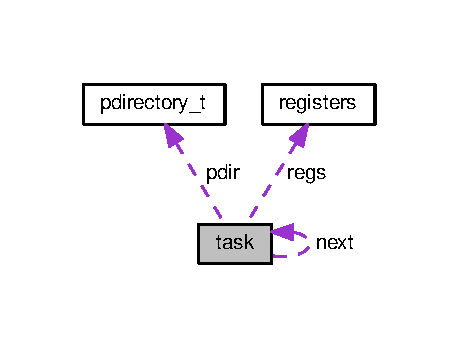
\includegraphics[width=220pt]{structtask__coll__graph}
\end{center}
\end{figure}
\subsection*{Data Fields}
\begin{DoxyCompactItemize}
\item 
int \hyperlink{structtask_a22d3a20ff225043177b269ec1a0a5f1a}{id}
\item 
char $\ast$ \hyperlink{structtask_a9aef5dbd16cfbbdb0c8b13416549a07f}{name}
\item 
\hyperlink{common_8h_adf58dbaf6139b4957c348711f2026957}{registers\+\_\+t} \hyperlink{structtask_a682bd33719ea3bc948375a5c51e91e4b}{regs}
\item 
uint32\+\_\+t \hyperlink{structtask_a9a1171f8e45d2c08d5a70290b94c5a6f}{Stack\+Top}
\item 
uint32\+\_\+t \hyperlink{structtask_aa7479c4cde3fed5f6c19fbc857112310}{ds}
\item 
uint32\+\_\+t \hyperlink{structtask_a95a59f8605e8bda30d38f73b67af42cc}{es}
\item 
uint32\+\_\+t \hyperlink{structtask_a2cb171a9e5b5d739cad8b83dffd05be3}{fs}
\item 
uint32\+\_\+t \hyperlink{structtask_a711674cead4b90d23503f3dfba0a489e}{gs}
\item 
uint16\+\_\+t \hyperlink{structtask_ac62cef90688fbf752e32cebb122f178a}{priority}
\item 
uint16\+\_\+t \hyperlink{structtask_a533c24b91bc1238517c1c42b53b3b8f0}{level}
\item 
uint32\+\_\+t \hyperlink{structtask_a9acefcf2fef4e255ec63a180f8ba6aea}{ss}
\item 
\hyperlink{paging_8h_a681a136bf0b5fcccb0c77e91ad5ad7b9}{pdirectory} $\ast$ \hyperlink{structtask_a9c01e75ea4d3ddf248a78c9d70f50237}{pdir}
\item 
struct \hyperlink{structtask}{task} $\ast$ \hyperlink{structtask_a3f2c7149983c28824baf1aebdfa7af98}{next}
\end{DoxyCompactItemize}


\subsection{Detailed Description}


Definition at line 17 of file task.\+h.



\subsection{Field Documentation}
\index{task@{task}!ds@{ds}}
\index{ds@{ds}!task@{task}}
\subsubsection[{\texorpdfstring{ds}{ds}}]{\setlength{\rightskip}{0pt plus 5cm}uint32\+\_\+t task\+::ds}\hypertarget{structtask_aa7479c4cde3fed5f6c19fbc857112310}{}\label{structtask_aa7479c4cde3fed5f6c19fbc857112310}


Definition at line 22 of file task.\+h.

\index{task@{task}!es@{es}}
\index{es@{es}!task@{task}}
\subsubsection[{\texorpdfstring{es}{es}}]{\setlength{\rightskip}{0pt plus 5cm}uint32\+\_\+t task\+::es}\hypertarget{structtask_a95a59f8605e8bda30d38f73b67af42cc}{}\label{structtask_a95a59f8605e8bda30d38f73b67af42cc}


Definition at line 22 of file task.\+h.

\index{task@{task}!fs@{fs}}
\index{fs@{fs}!task@{task}}
\subsubsection[{\texorpdfstring{fs}{fs}}]{\setlength{\rightskip}{0pt plus 5cm}uint32\+\_\+t task\+::fs}\hypertarget{structtask_a2cb171a9e5b5d739cad8b83dffd05be3}{}\label{structtask_a2cb171a9e5b5d739cad8b83dffd05be3}


Definition at line 22 of file task.\+h.

\index{task@{task}!gs@{gs}}
\index{gs@{gs}!task@{task}}
\subsubsection[{\texorpdfstring{gs}{gs}}]{\setlength{\rightskip}{0pt plus 5cm}uint32\+\_\+t task\+::gs}\hypertarget{structtask_a711674cead4b90d23503f3dfba0a489e}{}\label{structtask_a711674cead4b90d23503f3dfba0a489e}


Definition at line 22 of file task.\+h.

\index{task@{task}!id@{id}}
\index{id@{id}!task@{task}}
\subsubsection[{\texorpdfstring{id}{id}}]{\setlength{\rightskip}{0pt plus 5cm}int task\+::id}\hypertarget{structtask_a22d3a20ff225043177b269ec1a0a5f1a}{}\label{structtask_a22d3a20ff225043177b269ec1a0a5f1a}


Definition at line 19 of file task.\+h.

\index{task@{task}!level@{level}}
\index{level@{level}!task@{task}}
\subsubsection[{\texorpdfstring{level}{level}}]{\setlength{\rightskip}{0pt plus 5cm}uint16\+\_\+t task\+::level}\hypertarget{structtask_a533c24b91bc1238517c1c42b53b3b8f0}{}\label{structtask_a533c24b91bc1238517c1c42b53b3b8f0}


Definition at line 23 of file task.\+h.

\index{task@{task}!name@{name}}
\index{name@{name}!task@{task}}
\subsubsection[{\texorpdfstring{name}{name}}]{\setlength{\rightskip}{0pt plus 5cm}char$\ast$ task\+::name}\hypertarget{structtask_a9aef5dbd16cfbbdb0c8b13416549a07f}{}\label{structtask_a9aef5dbd16cfbbdb0c8b13416549a07f}


Definition at line 20 of file task.\+h.

\index{task@{task}!next@{next}}
\index{next@{next}!task@{task}}
\subsubsection[{\texorpdfstring{next}{next}}]{\setlength{\rightskip}{0pt plus 5cm}struct {\bf task}$\ast$ task\+::next}\hypertarget{structtask_a3f2c7149983c28824baf1aebdfa7af98}{}\label{structtask_a3f2c7149983c28824baf1aebdfa7af98}


Definition at line 26 of file task.\+h.

\index{task@{task}!pdir@{pdir}}
\index{pdir@{pdir}!task@{task}}
\subsubsection[{\texorpdfstring{pdir}{pdir}}]{\setlength{\rightskip}{0pt plus 5cm}{\bf pdirectory}$\ast$ task\+::pdir}\hypertarget{structtask_a9c01e75ea4d3ddf248a78c9d70f50237}{}\label{structtask_a9c01e75ea4d3ddf248a78c9d70f50237}


Definition at line 25 of file task.\+h.

\index{task@{task}!priority@{priority}}
\index{priority@{priority}!task@{task}}
\subsubsection[{\texorpdfstring{priority}{priority}}]{\setlength{\rightskip}{0pt plus 5cm}uint16\+\_\+t task\+::priority}\hypertarget{structtask_ac62cef90688fbf752e32cebb122f178a}{}\label{structtask_ac62cef90688fbf752e32cebb122f178a}


Definition at line 23 of file task.\+h.

\index{task@{task}!regs@{regs}}
\index{regs@{regs}!task@{task}}
\subsubsection[{\texorpdfstring{regs}{regs}}]{\setlength{\rightskip}{0pt plus 5cm}{\bf registers\+\_\+t} task\+::regs}\hypertarget{structtask_a682bd33719ea3bc948375a5c51e91e4b}{}\label{structtask_a682bd33719ea3bc948375a5c51e91e4b}


Definition at line 21 of file task.\+h.

\index{task@{task}!ss@{ss}}
\index{ss@{ss}!task@{task}}
\subsubsection[{\texorpdfstring{ss}{ss}}]{\setlength{\rightskip}{0pt plus 5cm}uint32\+\_\+t task\+::ss}\hypertarget{structtask_a9acefcf2fef4e255ec63a180f8ba6aea}{}\label{structtask_a9acefcf2fef4e255ec63a180f8ba6aea}


Definition at line 24 of file task.\+h.

\index{task@{task}!Stack\+Top@{Stack\+Top}}
\index{Stack\+Top@{Stack\+Top}!task@{task}}
\subsubsection[{\texorpdfstring{Stack\+Top}{StackTop}}]{\setlength{\rightskip}{0pt plus 5cm}uint32\+\_\+t task\+::\+Stack\+Top}\hypertarget{structtask_a9a1171f8e45d2c08d5a70290b94c5a6f}{}\label{structtask_a9a1171f8e45d2c08d5a70290b94c5a6f}


Definition at line 22 of file task.\+h.



The documentation for this struct was generated from the following file\+:\begin{DoxyCompactItemize}
\item 
Experimental Edition/\+Source/\+Multi\+Tasking/\hyperlink{task_8h}{task.\+h}\end{DoxyCompactItemize}

\hypertarget{structVESA__INFO}{}\section{V\+E\+S\+A\+\_\+\+I\+N\+FO Struct Reference}
\label{structVESA__INFO}\index{V\+E\+S\+A\+\_\+\+I\+N\+FO@{V\+E\+S\+A\+\_\+\+I\+N\+FO}}
\subsection*{Public Member Functions}
\begin{DoxyCompactItemize}
\item 
unsigned short V\+E\+S\+A\+Version \hyperlink{structVESA__INFO_ab14eb7a68b9de88409983f8bc6f79b64}{\+\_\+\+\_\+attribute\+\_\+\+\_\+} ((packed))
\item 
unsigned long O\+E\+M\+String\+Ptr \hyperlink{structVESA__INFO_a922a9b093cb718083725ddfd86f9285b}{\+\_\+\+\_\+attribute\+\_\+\+\_\+} ((packed))
\item 
unsigned long Video\+Mode\+Ptr \hyperlink{structVESA__INFO_a9d7b6d933201c8c12672214450d858a0}{\+\_\+\+\_\+attribute\+\_\+\+\_\+} ((packed))
\item 
unsigned short Total\+Memory \hyperlink{structVESA__INFO_a6e1cc548c457c54005c0116386a1b4a6}{\+\_\+\+\_\+attribute\+\_\+\+\_\+} ((packed))
\item 
unsigned short Oem\+Software\+Rev \hyperlink{structVESA__INFO_a566be4a4dd3ba397219aff084810f2e7}{\+\_\+\+\_\+attribute\+\_\+\+\_\+} ((packed))
\item 
unsigned long Oem\+Vendor\+Name\+Ptr \hyperlink{structVESA__INFO_a231abb3e5be2997bfdc7fe1dc621c309}{\+\_\+\+\_\+attribute\+\_\+\+\_\+} ((packed))
\item 
unsigned long Oem\+Product\+Name\+Ptr \hyperlink{structVESA__INFO_a45c3557b3f3b45d819de8a750980938b}{\+\_\+\+\_\+attribute\+\_\+\+\_\+} ((packed))
\item 
unsigned long Oem\+Product\+Rev\+Ptr \hyperlink{structVESA__INFO_a4b96a07f6c3ce3ba7efce50bcbc333fe}{\+\_\+\+\_\+attribute\+\_\+\+\_\+} ((packed))
\end{DoxyCompactItemize}
\subsection*{Data Fields}
\begin{DoxyCompactItemize}
\item 
unsigned char \hyperlink{structVESA__INFO_a29513615169621c4e98f3423197a4af2}{V\+E\+S\+A\+Signature} \mbox{[}4\mbox{]}
\item 
unsigned char \hyperlink{structVESA__INFO_ad758672d9e52736faab1d46d9d39c29a}{Capabilities} \mbox{[}4\mbox{]}
\item 
unsigned char \hyperlink{structVESA__INFO_aa2b5b63d3b2d14b3abbd73f749e07fa5}{Reserved} \mbox{[}222\mbox{]}
\item 
unsigned char \hyperlink{structVESA__INFO_a46a8c524e362968b69202f7210bac1e4}{Oem\+Data} \mbox{[}256\mbox{]}
\end{DoxyCompactItemize}


\subsection{Detailed Description}


Definition at line 60 of file vesa.\+c.



\subsection{Member Function Documentation}
\index{V\+E\+S\+A\+\_\+\+I\+N\+FO@{V\+E\+S\+A\+\_\+\+I\+N\+FO}!\+\_\+\+\_\+attribute\+\_\+\+\_\+@{\+\_\+\+\_\+attribute\+\_\+\+\_\+}}
\index{\+\_\+\+\_\+attribute\+\_\+\+\_\+@{\+\_\+\+\_\+attribute\+\_\+\+\_\+}!V\+E\+S\+A\+\_\+\+I\+N\+FO@{V\+E\+S\+A\+\_\+\+I\+N\+FO}}
\subsubsection[{\texorpdfstring{\+\_\+\+\_\+attribute\+\_\+\+\_\+((packed))}{__attribute__((packed))}}]{\setlength{\rightskip}{0pt plus 5cm}unsigned short V\+E\+S\+A\+Version V\+E\+S\+A\+\_\+\+I\+N\+F\+O\+::\+\_\+\+\_\+attribute\+\_\+\+\_\+ (
\begin{DoxyParamCaption}
\item[{(packed)}]{}
\end{DoxyParamCaption}
)}\hypertarget{structVESA__INFO_ab14eb7a68b9de88409983f8bc6f79b64}{}\label{structVESA__INFO_ab14eb7a68b9de88409983f8bc6f79b64}
\index{V\+E\+S\+A\+\_\+\+I\+N\+FO@{V\+E\+S\+A\+\_\+\+I\+N\+FO}!\+\_\+\+\_\+attribute\+\_\+\+\_\+@{\+\_\+\+\_\+attribute\+\_\+\+\_\+}}
\index{\+\_\+\+\_\+attribute\+\_\+\+\_\+@{\+\_\+\+\_\+attribute\+\_\+\+\_\+}!V\+E\+S\+A\+\_\+\+I\+N\+FO@{V\+E\+S\+A\+\_\+\+I\+N\+FO}}
\subsubsection[{\texorpdfstring{\+\_\+\+\_\+attribute\+\_\+\+\_\+((packed))}{__attribute__((packed))}}]{\setlength{\rightskip}{0pt plus 5cm}unsigned long O\+E\+M\+String\+Ptr V\+E\+S\+A\+\_\+\+I\+N\+F\+O\+::\+\_\+\+\_\+attribute\+\_\+\+\_\+ (
\begin{DoxyParamCaption}
\item[{(packed)}]{}
\end{DoxyParamCaption}
)}\hypertarget{structVESA__INFO_a922a9b093cb718083725ddfd86f9285b}{}\label{structVESA__INFO_a922a9b093cb718083725ddfd86f9285b}
\index{V\+E\+S\+A\+\_\+\+I\+N\+FO@{V\+E\+S\+A\+\_\+\+I\+N\+FO}!\+\_\+\+\_\+attribute\+\_\+\+\_\+@{\+\_\+\+\_\+attribute\+\_\+\+\_\+}}
\index{\+\_\+\+\_\+attribute\+\_\+\+\_\+@{\+\_\+\+\_\+attribute\+\_\+\+\_\+}!V\+E\+S\+A\+\_\+\+I\+N\+FO@{V\+E\+S\+A\+\_\+\+I\+N\+FO}}
\subsubsection[{\texorpdfstring{\+\_\+\+\_\+attribute\+\_\+\+\_\+((packed))}{__attribute__((packed))}}]{\setlength{\rightskip}{0pt plus 5cm}unsigned long Video\+Mode\+Ptr V\+E\+S\+A\+\_\+\+I\+N\+F\+O\+::\+\_\+\+\_\+attribute\+\_\+\+\_\+ (
\begin{DoxyParamCaption}
\item[{(packed)}]{}
\end{DoxyParamCaption}
)}\hypertarget{structVESA__INFO_a9d7b6d933201c8c12672214450d858a0}{}\label{structVESA__INFO_a9d7b6d933201c8c12672214450d858a0}
\index{V\+E\+S\+A\+\_\+\+I\+N\+FO@{V\+E\+S\+A\+\_\+\+I\+N\+FO}!\+\_\+\+\_\+attribute\+\_\+\+\_\+@{\+\_\+\+\_\+attribute\+\_\+\+\_\+}}
\index{\+\_\+\+\_\+attribute\+\_\+\+\_\+@{\+\_\+\+\_\+attribute\+\_\+\+\_\+}!V\+E\+S\+A\+\_\+\+I\+N\+FO@{V\+E\+S\+A\+\_\+\+I\+N\+FO}}
\subsubsection[{\texorpdfstring{\+\_\+\+\_\+attribute\+\_\+\+\_\+((packed))}{__attribute__((packed))}}]{\setlength{\rightskip}{0pt plus 5cm}unsigned short Total\+Memory V\+E\+S\+A\+\_\+\+I\+N\+F\+O\+::\+\_\+\+\_\+attribute\+\_\+\+\_\+ (
\begin{DoxyParamCaption}
\item[{(packed)}]{}
\end{DoxyParamCaption}
)}\hypertarget{structVESA__INFO_a6e1cc548c457c54005c0116386a1b4a6}{}\label{structVESA__INFO_a6e1cc548c457c54005c0116386a1b4a6}
\index{V\+E\+S\+A\+\_\+\+I\+N\+FO@{V\+E\+S\+A\+\_\+\+I\+N\+FO}!\+\_\+\+\_\+attribute\+\_\+\+\_\+@{\+\_\+\+\_\+attribute\+\_\+\+\_\+}}
\index{\+\_\+\+\_\+attribute\+\_\+\+\_\+@{\+\_\+\+\_\+attribute\+\_\+\+\_\+}!V\+E\+S\+A\+\_\+\+I\+N\+FO@{V\+E\+S\+A\+\_\+\+I\+N\+FO}}
\subsubsection[{\texorpdfstring{\+\_\+\+\_\+attribute\+\_\+\+\_\+((packed))}{__attribute__((packed))}}]{\setlength{\rightskip}{0pt plus 5cm}unsigned short Oem\+Software\+Rev V\+E\+S\+A\+\_\+\+I\+N\+F\+O\+::\+\_\+\+\_\+attribute\+\_\+\+\_\+ (
\begin{DoxyParamCaption}
\item[{(packed)}]{}
\end{DoxyParamCaption}
)}\hypertarget{structVESA__INFO_a566be4a4dd3ba397219aff084810f2e7}{}\label{structVESA__INFO_a566be4a4dd3ba397219aff084810f2e7}
\index{V\+E\+S\+A\+\_\+\+I\+N\+FO@{V\+E\+S\+A\+\_\+\+I\+N\+FO}!\+\_\+\+\_\+attribute\+\_\+\+\_\+@{\+\_\+\+\_\+attribute\+\_\+\+\_\+}}
\index{\+\_\+\+\_\+attribute\+\_\+\+\_\+@{\+\_\+\+\_\+attribute\+\_\+\+\_\+}!V\+E\+S\+A\+\_\+\+I\+N\+FO@{V\+E\+S\+A\+\_\+\+I\+N\+FO}}
\subsubsection[{\texorpdfstring{\+\_\+\+\_\+attribute\+\_\+\+\_\+((packed))}{__attribute__((packed))}}]{\setlength{\rightskip}{0pt plus 5cm}unsigned long Oem\+Vendor\+Name\+Ptr V\+E\+S\+A\+\_\+\+I\+N\+F\+O\+::\+\_\+\+\_\+attribute\+\_\+\+\_\+ (
\begin{DoxyParamCaption}
\item[{(packed)}]{}
\end{DoxyParamCaption}
)}\hypertarget{structVESA__INFO_a231abb3e5be2997bfdc7fe1dc621c309}{}\label{structVESA__INFO_a231abb3e5be2997bfdc7fe1dc621c309}
\index{V\+E\+S\+A\+\_\+\+I\+N\+FO@{V\+E\+S\+A\+\_\+\+I\+N\+FO}!\+\_\+\+\_\+attribute\+\_\+\+\_\+@{\+\_\+\+\_\+attribute\+\_\+\+\_\+}}
\index{\+\_\+\+\_\+attribute\+\_\+\+\_\+@{\+\_\+\+\_\+attribute\+\_\+\+\_\+}!V\+E\+S\+A\+\_\+\+I\+N\+FO@{V\+E\+S\+A\+\_\+\+I\+N\+FO}}
\subsubsection[{\texorpdfstring{\+\_\+\+\_\+attribute\+\_\+\+\_\+((packed))}{__attribute__((packed))}}]{\setlength{\rightskip}{0pt plus 5cm}unsigned long Oem\+Product\+Name\+Ptr V\+E\+S\+A\+\_\+\+I\+N\+F\+O\+::\+\_\+\+\_\+attribute\+\_\+\+\_\+ (
\begin{DoxyParamCaption}
\item[{(packed)}]{}
\end{DoxyParamCaption}
)}\hypertarget{structVESA__INFO_a45c3557b3f3b45d819de8a750980938b}{}\label{structVESA__INFO_a45c3557b3f3b45d819de8a750980938b}
\index{V\+E\+S\+A\+\_\+\+I\+N\+FO@{V\+E\+S\+A\+\_\+\+I\+N\+FO}!\+\_\+\+\_\+attribute\+\_\+\+\_\+@{\+\_\+\+\_\+attribute\+\_\+\+\_\+}}
\index{\+\_\+\+\_\+attribute\+\_\+\+\_\+@{\+\_\+\+\_\+attribute\+\_\+\+\_\+}!V\+E\+S\+A\+\_\+\+I\+N\+FO@{V\+E\+S\+A\+\_\+\+I\+N\+FO}}
\subsubsection[{\texorpdfstring{\+\_\+\+\_\+attribute\+\_\+\+\_\+((packed))}{__attribute__((packed))}}]{\setlength{\rightskip}{0pt plus 5cm}unsigned long Oem\+Product\+Rev\+Ptr V\+E\+S\+A\+\_\+\+I\+N\+F\+O\+::\+\_\+\+\_\+attribute\+\_\+\+\_\+ (
\begin{DoxyParamCaption}
\item[{(packed)}]{}
\end{DoxyParamCaption}
)}\hypertarget{structVESA__INFO_a4b96a07f6c3ce3ba7efce50bcbc333fe}{}\label{structVESA__INFO_a4b96a07f6c3ce3ba7efce50bcbc333fe}


\subsection{Field Documentation}
\index{V\+E\+S\+A\+\_\+\+I\+N\+FO@{V\+E\+S\+A\+\_\+\+I\+N\+FO}!Capabilities@{Capabilities}}
\index{Capabilities@{Capabilities}!V\+E\+S\+A\+\_\+\+I\+N\+FO@{V\+E\+S\+A\+\_\+\+I\+N\+FO}}
\subsubsection[{\texorpdfstring{Capabilities}{Capabilities}}]{\setlength{\rightskip}{0pt plus 5cm}unsigned char V\+E\+S\+A\+\_\+\+I\+N\+F\+O\+::\+Capabilities\mbox{[}4\mbox{]}}\hypertarget{structVESA__INFO_ad758672d9e52736faab1d46d9d39c29a}{}\label{structVESA__INFO_ad758672d9e52736faab1d46d9d39c29a}


Definition at line 65 of file vesa.\+c.

\index{V\+E\+S\+A\+\_\+\+I\+N\+FO@{V\+E\+S\+A\+\_\+\+I\+N\+FO}!Oem\+Data@{Oem\+Data}}
\index{Oem\+Data@{Oem\+Data}!V\+E\+S\+A\+\_\+\+I\+N\+FO@{V\+E\+S\+A\+\_\+\+I\+N\+FO}}
\subsubsection[{\texorpdfstring{Oem\+Data}{OemData}}]{\setlength{\rightskip}{0pt plus 5cm}unsigned char V\+E\+S\+A\+\_\+\+I\+N\+F\+O\+::\+Oem\+Data\mbox{[}256\mbox{]}}\hypertarget{structVESA__INFO_a46a8c524e362968b69202f7210bac1e4}{}\label{structVESA__INFO_a46a8c524e362968b69202f7210bac1e4}


Definition at line 73 of file vesa.\+c.

\index{V\+E\+S\+A\+\_\+\+I\+N\+FO@{V\+E\+S\+A\+\_\+\+I\+N\+FO}!Reserved@{Reserved}}
\index{Reserved@{Reserved}!V\+E\+S\+A\+\_\+\+I\+N\+FO@{V\+E\+S\+A\+\_\+\+I\+N\+FO}}
\subsubsection[{\texorpdfstring{Reserved}{Reserved}}]{\setlength{\rightskip}{0pt plus 5cm}unsigned char V\+E\+S\+A\+\_\+\+I\+N\+F\+O\+::\+Reserved\mbox{[}222\mbox{]}}\hypertarget{structVESA__INFO_aa2b5b63d3b2d14b3abbd73f749e07fa5}{}\label{structVESA__INFO_aa2b5b63d3b2d14b3abbd73f749e07fa5}


Definition at line 72 of file vesa.\+c.

\index{V\+E\+S\+A\+\_\+\+I\+N\+FO@{V\+E\+S\+A\+\_\+\+I\+N\+FO}!V\+E\+S\+A\+Signature@{V\+E\+S\+A\+Signature}}
\index{V\+E\+S\+A\+Signature@{V\+E\+S\+A\+Signature}!V\+E\+S\+A\+\_\+\+I\+N\+FO@{V\+E\+S\+A\+\_\+\+I\+N\+FO}}
\subsubsection[{\texorpdfstring{V\+E\+S\+A\+Signature}{VESASignature}}]{\setlength{\rightskip}{0pt plus 5cm}unsigned char V\+E\+S\+A\+\_\+\+I\+N\+F\+O\+::\+V\+E\+S\+A\+Signature\mbox{[}4\mbox{]}}\hypertarget{structVESA__INFO_a29513615169621c4e98f3423197a4af2}{}\label{structVESA__INFO_a29513615169621c4e98f3423197a4af2}


Definition at line 62 of file vesa.\+c.



The documentation for this struct was generated from the following file\+:\begin{DoxyCompactItemize}
\item 
Experimental Edition/\+Source/vesa/\hyperlink{vesa_8c}{vesa.\+c}\end{DoxyCompactItemize}

\chapter{File Documentation}
\hypertarget{abc_8h}{}\section{Experimental Edition/\+Library/abc.h File Reference}
\label{abc_8h}\index{Experimental Edition/\+Library/abc.\+h@{Experimental Edition/\+Library/abc.\+h}}
{\ttfamily \#include $<$common.\+h$>$}\\*
Include dependency graph for abc.\+h\+:
\nopagebreak
\begin{figure}[H]
\begin{center}
\leavevmode
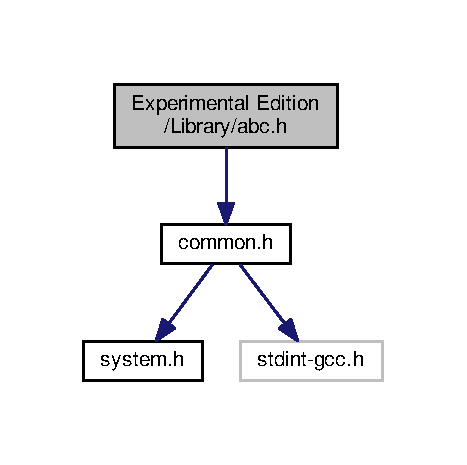
\includegraphics[width=224pt]{abc_8h__incl}
\end{center}
\end{figure}
\subsection*{Variables}
\begin{DoxyCompactItemize}
\item 
\hyperlink{common_8h_a7ae3a26c17ddfe117c6291739780801d}{u32int} \hyperlink{abc_8h_a6342e29537636642d9a1477deabf683f}{end}
\end{DoxyCompactItemize}


\subsection{Variable Documentation}
\index{abc.\+h@{abc.\+h}!end@{end}}
\index{end@{end}!abc.\+h@{abc.\+h}}
\subsubsection[{\texorpdfstring{end}{end}}]{\setlength{\rightskip}{0pt plus 5cm}{\bf u32int} end}\hypertarget{abc_8h_a6342e29537636642d9a1477deabf683f}{}\label{abc_8h_a6342e29537636642d9a1477deabf683f}

\hypertarget{assert_8h}{}\section{Experimental Edition/\+Library/assert.h File Reference}
\label{assert_8h}\index{Experimental Edition/\+Library/assert.\+h@{Experimental Edition/\+Library/assert.\+h}}
\subsection*{Macros}
\begin{DoxyCompactItemize}
\item 
\#define \hyperlink{assert_8h_ae90784e7cdd9af82802f90079c4e64e8}{assert}(ignore)~((void)0)
\end{DoxyCompactItemize}


\subsection{Macro Definition Documentation}
\index{assert.\+h@{assert.\+h}!assert@{assert}}
\index{assert@{assert}!assert.\+h@{assert.\+h}}
\subsubsection[{\texorpdfstring{assert}{assert}}]{\setlength{\rightskip}{0pt plus 5cm}\#define assert(
\begin{DoxyParamCaption}
\item[{}]{ignore}
\end{DoxyParamCaption}
)~((void)0)}\hypertarget{assert_8h_ae90784e7cdd9af82802f90079c4e64e8}{}\label{assert_8h_ae90784e7cdd9af82802f90079c4e64e8}


Definition at line 4 of file assert.\+h.


\hypertarget{common_8h}{}\section{Experimental Edition/\+Library/common.h File Reference}
\label{common_8h}\index{Experimental Edition/\+Library/common.\+h@{Experimental Edition/\+Library/common.\+h}}
{\ttfamily \#include $<$system.\+h$>$}\\*
{\ttfamily \#include $<$stdint-\/gcc.\+h$>$}\\*
Include dependency graph for common.\+h\+:
\nopagebreak
\begin{figure}[H]
\begin{center}
\leavevmode
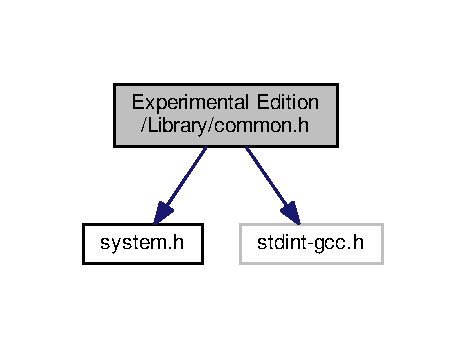
\includegraphics[width=224pt]{common_8h__incl}
\end{center}
\end{figure}
This graph shows which files directly or indirectly include this file\+:
\nopagebreak
\begin{figure}[H]
\begin{center}
\leavevmode
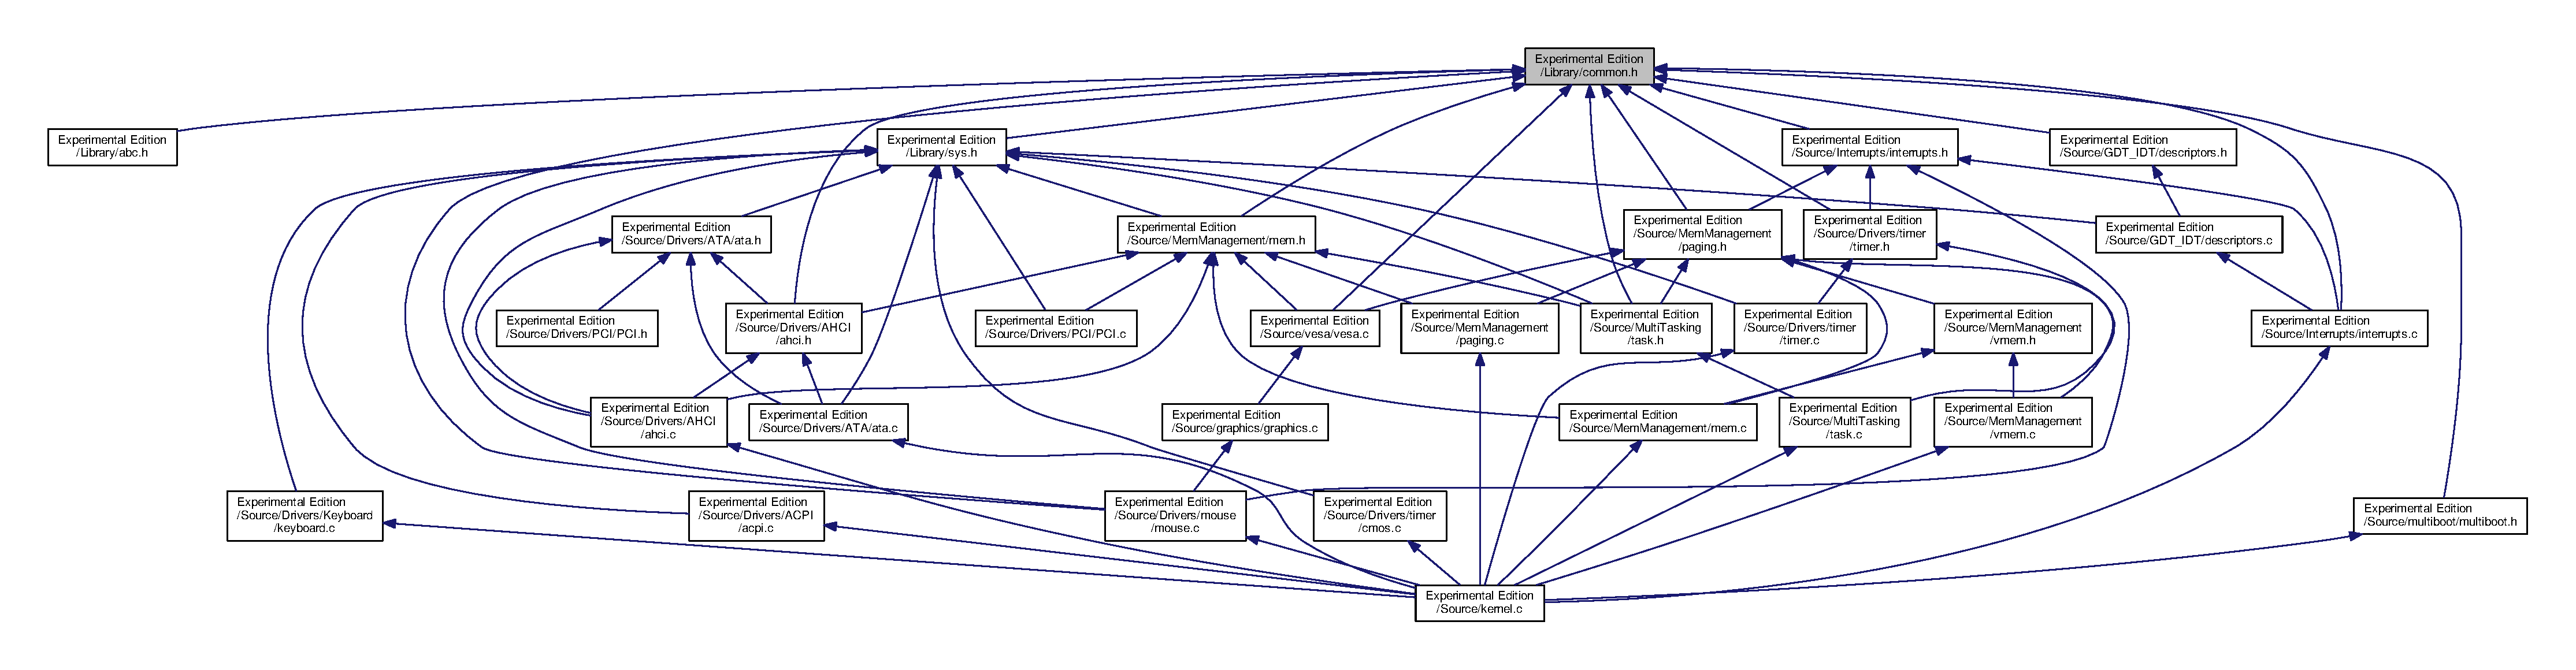
\includegraphics[width=350pt]{common_8h__dep__incl}
\end{center}
\end{figure}
\subsection*{Data Structures}
\begin{DoxyCompactItemize}
\item 
struct \hyperlink{structfile}{file}
\item 
struct \hyperlink{structregisters}{registers}
\end{DoxyCompactItemize}
\subsection*{Macros}
\begin{DoxyCompactItemize}
\item 
\#define \hyperlink{common_8h_a070d2ce7b6bb7e5c05602aa8c308d0c4}{N\+U\+LL}~((void$\ast$) 0)
\item 
\#define \hyperlink{common_8h_a926c1ab4f6ca8b244750377dcdea9ec1}{M\+IN}(\+\_\+a,  \+\_\+b)
\item 
\#define \hyperlink{common_8h_ad448d437b99a125bd9344585d4f02e9a}{M\+AX}(\+\_\+a,  \+\_\+b)
\item 
\#define \hyperlink{common_8h_a057810d35075597ca699719778344515}{R\+O\+U\+N\+D\+D\+O\+WN}(a,  n)
\item 
\#define \hyperlink{common_8h_a5d25fbed833545ed7a3c01e818de0bcf}{R\+O\+U\+N\+D\+UP}(a,  n)
\item 
\#define \hyperlink{common_8h_afd049f7ad59dbe455f460807475c2841}{offsetof}(type,  member)~((size\+\_\+t) (\&((type$\ast$)0)-\/$>$member))
\item 
\#define \hyperlink{common_8h_a0d112bae8fd35be772185b6ec6bcbe64}{S\+E\+E\+K\+\_\+\+S\+ET}~1
\item 
\#define \hyperlink{common_8h_a4c8d0b76b470ba65a43ca46a88320f39}{S\+E\+E\+K\+\_\+\+C\+UR}~2
\item 
\#define \hyperlink{common_8h_ad2a2e6c114780c3071efd24f16c7f7d8}{S\+E\+E\+K\+\_\+\+E\+ND}~3
\item 
\#define \hyperlink{common_8h_a101586fab2b90a8adffe50a3550e235d}{A\+S\+S\+E\+RT}(b)~((b) ? (void)0 \+: panic\+\_\+assert(\+\_\+\+\_\+\+F\+I\+L\+E\+\_\+\+\_\+, \+\_\+\+\_\+\+L\+I\+N\+E\+\_\+\+\_\+, \#b))
\end{DoxyCompactItemize}
\subsection*{Typedefs}
\begin{DoxyCompactItemize}
\item 
typedef uint32\+\_\+t \hyperlink{common_8h_a7ae3a26c17ddfe117c6291739780801d}{u32int}
\item 
typedef int \hyperlink{common_8h_a61350201bbcea1180bb1160bd09b717f}{s32int}
\item 
typedef uint16\+\_\+t \hyperlink{common_8h_ade81be9b965e7be1641f9792ba8af75e}{u16int}
\item 
typedef short \hyperlink{common_8h_ad039e929f72cfdb80d3a96ac1f7d9c3d}{s16int}
\item 
typedef uint8\+\_\+t \hyperlink{common_8h_a27a416e6606c138f2d33233142a5593e}{u8int}
\item 
typedef char \hyperlink{common_8h_afa805b2bbcb6f0e85de57cef336f98df}{s8int}
\item 
typedef \+\_\+\+Bool \hyperlink{common_8h_afaa87723b8417d40fcf45b7330261ef9}{bool}
\item 
typedef struct \hyperlink{structregisters}{registers} \hyperlink{common_8h_adf58dbaf6139b4957c348711f2026957}{registers\+\_\+t}
\item 
typedef void($\ast$ \hyperlink{common_8h_a0468dc495af5789aa4d49f2d4d0ede0d}{isr\+\_\+t}) (\hyperlink{common_8h_adf58dbaf6139b4957c348711f2026957}{registers\+\_\+t})
\item 
typedef void($\ast$ \hyperlink{common_8h_a4e754d9618c8c45cd58f7e9b6638a906}{irq\+\_\+t}) ()
\end{DoxyCompactItemize}
\subsection*{Enumerations}
\begin{DoxyCompactItemize}
\item 
enum \{ \hyperlink{common_8h_a06fc87d81c62e9abb8790b6e5713c55bae9de385ef6fe9bf3360d1038396b884c}{false}, 
\hyperlink{common_8h_a06fc87d81c62e9abb8790b6e5713c55ba08f175a5505a10b9ed657defeb050e4b}{true}
 \}
\end{DoxyCompactItemize}


\subsection{Macro Definition Documentation}
\index{common.\+h@{common.\+h}!A\+S\+S\+E\+RT@{A\+S\+S\+E\+RT}}
\index{A\+S\+S\+E\+RT@{A\+S\+S\+E\+RT}!common.\+h@{common.\+h}}
\subsubsection[{\texorpdfstring{A\+S\+S\+E\+RT}{ASSERT}}]{\setlength{\rightskip}{0pt plus 5cm}\#define A\+S\+S\+E\+RT(
\begin{DoxyParamCaption}
\item[{}]{b}
\end{DoxyParamCaption}
)~((b) ? (void)0 \+: panic\+\_\+assert(\+\_\+\+\_\+\+F\+I\+L\+E\+\_\+\+\_\+, \+\_\+\+\_\+\+L\+I\+N\+E\+\_\+\+\_\+, \#b))}\hypertarget{common_8h_a101586fab2b90a8adffe50a3550e235d}{}\label{common_8h_a101586fab2b90a8adffe50a3550e235d}


Definition at line 84 of file common.\+h.

\index{common.\+h@{common.\+h}!M\+AX@{M\+AX}}
\index{M\+AX@{M\+AX}!common.\+h@{common.\+h}}
\subsubsection[{\texorpdfstring{M\+AX}{MAX}}]{\setlength{\rightskip}{0pt plus 5cm}\#define M\+AX(
\begin{DoxyParamCaption}
\item[{}]{\+\_\+a, }
\item[{}]{\+\_\+b}
\end{DoxyParamCaption}
)}\hypertarget{common_8h_ad448d437b99a125bd9344585d4f02e9a}{}\label{common_8h_ad448d437b99a125bd9344585d4f02e9a}
{\bfseries Value\+:}
\begin{DoxyCode}
(\{                              \(\backslash\)
    typeof(\_a) \_\_a = (\_a);                  \(\backslash\)
    typeof(\_b) \_\_b = (\_b);                  \(\backslash\)
    \_\_a >= \_\_b ? \_\_a : \_\_b;                 \(\backslash\)
\})
\end{DoxyCode}


Definition at line 32 of file common.\+h.

\index{common.\+h@{common.\+h}!M\+IN@{M\+IN}}
\index{M\+IN@{M\+IN}!common.\+h@{common.\+h}}
\subsubsection[{\texorpdfstring{M\+IN}{MIN}}]{\setlength{\rightskip}{0pt plus 5cm}\#define M\+IN(
\begin{DoxyParamCaption}
\item[{}]{\+\_\+a, }
\item[{}]{\+\_\+b}
\end{DoxyParamCaption}
)}\hypertarget{common_8h_a926c1ab4f6ca8b244750377dcdea9ec1}{}\label{common_8h_a926c1ab4f6ca8b244750377dcdea9ec1}
{\bfseries Value\+:}
\begin{DoxyCode}
(\{                              \(\backslash\)
    typeof(\_a) \_\_a = (\_a);                  \(\backslash\)
    typeof(\_b) \_\_b = (\_b);                  \(\backslash\)
    \_\_a <= \_\_b ? \_\_a : \_\_b;                 \(\backslash\)
\})
\end{DoxyCode}


Definition at line 26 of file common.\+h.

\index{common.\+h@{common.\+h}!N\+U\+LL@{N\+U\+LL}}
\index{N\+U\+LL@{N\+U\+LL}!common.\+h@{common.\+h}}
\subsubsection[{\texorpdfstring{N\+U\+LL}{NULL}}]{\setlength{\rightskip}{0pt plus 5cm}\#define N\+U\+LL~((void$\ast$) 0)}\hypertarget{common_8h_a070d2ce7b6bb7e5c05602aa8c308d0c4}{}\label{common_8h_a070d2ce7b6bb7e5c05602aa8c308d0c4}


Definition at line 18 of file common.\+h.

\index{common.\+h@{common.\+h}!offsetof@{offsetof}}
\index{offsetof@{offsetof}!common.\+h@{common.\+h}}
\subsubsection[{\texorpdfstring{offsetof}{offsetof}}]{\setlength{\rightskip}{0pt plus 5cm}\#define offsetof(
\begin{DoxyParamCaption}
\item[{}]{type, }
\item[{}]{member}
\end{DoxyParamCaption}
)~((size\+\_\+t) (\&((type$\ast$)0)-\/$>$member))}\hypertarget{common_8h_afd049f7ad59dbe455f460807475c2841}{}\label{common_8h_afd049f7ad59dbe455f460807475c2841}


Definition at line 54 of file common.\+h.

\index{common.\+h@{common.\+h}!R\+O\+U\+N\+D\+D\+O\+WN@{R\+O\+U\+N\+D\+D\+O\+WN}}
\index{R\+O\+U\+N\+D\+D\+O\+WN@{R\+O\+U\+N\+D\+D\+O\+WN}!common.\+h@{common.\+h}}
\subsubsection[{\texorpdfstring{R\+O\+U\+N\+D\+D\+O\+WN}{ROUNDDOWN}}]{\setlength{\rightskip}{0pt plus 5cm}\#define R\+O\+U\+N\+D\+D\+O\+WN(
\begin{DoxyParamCaption}
\item[{}]{a, }
\item[{}]{n}
\end{DoxyParamCaption}
)}\hypertarget{common_8h_a057810d35075597ca699719778344515}{}\label{common_8h_a057810d35075597ca699719778344515}
{\bfseries Value\+:}
\begin{DoxyCode}
(\{                              \(\backslash\)
    uint64\_t \_\_a = (uint64\_t) (a);              \(\backslash\)
    (typeof(a)) (\_\_a - \_\_a % (n));              \(\backslash\)
\})
\end{DoxyCode}


Definition at line 41 of file common.\+h.

\index{common.\+h@{common.\+h}!R\+O\+U\+N\+D\+UP@{R\+O\+U\+N\+D\+UP}}
\index{R\+O\+U\+N\+D\+UP@{R\+O\+U\+N\+D\+UP}!common.\+h@{common.\+h}}
\subsubsection[{\texorpdfstring{R\+O\+U\+N\+D\+UP}{ROUNDUP}}]{\setlength{\rightskip}{0pt plus 5cm}\#define R\+O\+U\+N\+D\+UP(
\begin{DoxyParamCaption}
\item[{}]{a, }
\item[{}]{n}
\end{DoxyParamCaption}
)}\hypertarget{common_8h_a5d25fbed833545ed7a3c01e818de0bcf}{}\label{common_8h_a5d25fbed833545ed7a3c01e818de0bcf}
{\bfseries Value\+:}
\begin{DoxyCode}
(\{                              \(\backslash\)
    uint64\_t \_\_n = (uint64\_t) (n);              \(\backslash\)
    (typeof(a)) (\hyperlink{common_8h_a057810d35075597ca699719778344515}{ROUNDDOWN}((uint64\_t) (a) + \_\_n - 1, \_\_n));    \(\backslash\)
\})
\end{DoxyCode}


Definition at line 47 of file common.\+h.

\index{common.\+h@{common.\+h}!S\+E\+E\+K\+\_\+\+C\+UR@{S\+E\+E\+K\+\_\+\+C\+UR}}
\index{S\+E\+E\+K\+\_\+\+C\+UR@{S\+E\+E\+K\+\_\+\+C\+UR}!common.\+h@{common.\+h}}
\subsubsection[{\texorpdfstring{S\+E\+E\+K\+\_\+\+C\+UR}{SEEK_CUR}}]{\setlength{\rightskip}{0pt plus 5cm}\#define S\+E\+E\+K\+\_\+\+C\+UR~2}\hypertarget{common_8h_a4c8d0b76b470ba65a43ca46a88320f39}{}\label{common_8h_a4c8d0b76b470ba65a43ca46a88320f39}


Definition at line 68 of file common.\+h.

\index{common.\+h@{common.\+h}!S\+E\+E\+K\+\_\+\+E\+ND@{S\+E\+E\+K\+\_\+\+E\+ND}}
\index{S\+E\+E\+K\+\_\+\+E\+ND@{S\+E\+E\+K\+\_\+\+E\+ND}!common.\+h@{common.\+h}}
\subsubsection[{\texorpdfstring{S\+E\+E\+K\+\_\+\+E\+ND}{SEEK_END}}]{\setlength{\rightskip}{0pt plus 5cm}\#define S\+E\+E\+K\+\_\+\+E\+ND~3}\hypertarget{common_8h_ad2a2e6c114780c3071efd24f16c7f7d8}{}\label{common_8h_ad2a2e6c114780c3071efd24f16c7f7d8}


Definition at line 69 of file common.\+h.

\index{common.\+h@{common.\+h}!S\+E\+E\+K\+\_\+\+S\+ET@{S\+E\+E\+K\+\_\+\+S\+ET}}
\index{S\+E\+E\+K\+\_\+\+S\+ET@{S\+E\+E\+K\+\_\+\+S\+ET}!common.\+h@{common.\+h}}
\subsubsection[{\texorpdfstring{S\+E\+E\+K\+\_\+\+S\+ET}{SEEK_SET}}]{\setlength{\rightskip}{0pt plus 5cm}\#define S\+E\+E\+K\+\_\+\+S\+ET~1}\hypertarget{common_8h_a0d112bae8fd35be772185b6ec6bcbe64}{}\label{common_8h_a0d112bae8fd35be772185b6ec6bcbe64}


Definition at line 67 of file common.\+h.



\subsection{Typedef Documentation}
\index{common.\+h@{common.\+h}!bool@{bool}}
\index{bool@{bool}!common.\+h@{common.\+h}}
\subsubsection[{\texorpdfstring{bool}{bool}}]{\setlength{\rightskip}{0pt plus 5cm}typedef \+\_\+\+Bool {\bf bool}}\hypertarget{common_8h_afaa87723b8417d40fcf45b7330261ef9}{}\label{common_8h_afaa87723b8417d40fcf45b7330261ef9}


Definition at line 22 of file common.\+h.

\index{common.\+h@{common.\+h}!irq\+\_\+t@{irq\+\_\+t}}
\index{irq\+\_\+t@{irq\+\_\+t}!common.\+h@{common.\+h}}
\subsubsection[{\texorpdfstring{irq\+\_\+t}{irq_t}}]{\setlength{\rightskip}{0pt plus 5cm}typedef void($\ast$ irq\+\_\+t) ()}\hypertarget{common_8h_a4e754d9618c8c45cd58f7e9b6638a906}{}\label{common_8h_a4e754d9618c8c45cd58f7e9b6638a906}


Definition at line 82 of file common.\+h.

\index{common.\+h@{common.\+h}!isr\+\_\+t@{isr\+\_\+t}}
\index{isr\+\_\+t@{isr\+\_\+t}!common.\+h@{common.\+h}}
\subsubsection[{\texorpdfstring{isr\+\_\+t}{isr_t}}]{\setlength{\rightskip}{0pt plus 5cm}typedef void($\ast$ isr\+\_\+t) ({\bf registers\+\_\+t})}\hypertarget{common_8h_a0468dc495af5789aa4d49f2d4d0ede0d}{}\label{common_8h_a0468dc495af5789aa4d49f2d4d0ede0d}


Definition at line 80 of file common.\+h.

\index{common.\+h@{common.\+h}!registers\+\_\+t@{registers\+\_\+t}}
\index{registers\+\_\+t@{registers\+\_\+t}!common.\+h@{common.\+h}}
\subsubsection[{\texorpdfstring{registers\+\_\+t}{registers_t}}]{\setlength{\rightskip}{0pt plus 5cm}typedef struct {\bf registers}  {\bf registers\+\_\+t}}\hypertarget{common_8h_adf58dbaf6139b4957c348711f2026957}{}\label{common_8h_adf58dbaf6139b4957c348711f2026957}
\index{common.\+h@{common.\+h}!s16int@{s16int}}
\index{s16int@{s16int}!common.\+h@{common.\+h}}
\subsubsection[{\texorpdfstring{s16int}{s16int}}]{\setlength{\rightskip}{0pt plus 5cm}typedef short {\bf s16int}}\hypertarget{common_8h_ad039e929f72cfdb80d3a96ac1f7d9c3d}{}\label{common_8h_ad039e929f72cfdb80d3a96ac1f7d9c3d}


Definition at line 13 of file common.\+h.

\index{common.\+h@{common.\+h}!s32int@{s32int}}
\index{s32int@{s32int}!common.\+h@{common.\+h}}
\subsubsection[{\texorpdfstring{s32int}{s32int}}]{\setlength{\rightskip}{0pt plus 5cm}typedef int {\bf s32int}}\hypertarget{common_8h_a61350201bbcea1180bb1160bd09b717f}{}\label{common_8h_a61350201bbcea1180bb1160bd09b717f}


Definition at line 11 of file common.\+h.

\index{common.\+h@{common.\+h}!s8int@{s8int}}
\index{s8int@{s8int}!common.\+h@{common.\+h}}
\subsubsection[{\texorpdfstring{s8int}{s8int}}]{\setlength{\rightskip}{0pt plus 5cm}typedef char {\bf s8int}}\hypertarget{common_8h_afa805b2bbcb6f0e85de57cef336f98df}{}\label{common_8h_afa805b2bbcb6f0e85de57cef336f98df}


Definition at line 15 of file common.\+h.

\index{common.\+h@{common.\+h}!u16int@{u16int}}
\index{u16int@{u16int}!common.\+h@{common.\+h}}
\subsubsection[{\texorpdfstring{u16int}{u16int}}]{\setlength{\rightskip}{0pt plus 5cm}typedef uint16\+\_\+t {\bf u16int}}\hypertarget{common_8h_ade81be9b965e7be1641f9792ba8af75e}{}\label{common_8h_ade81be9b965e7be1641f9792ba8af75e}


Definition at line 12 of file common.\+h.

\index{common.\+h@{common.\+h}!u32int@{u32int}}
\index{u32int@{u32int}!common.\+h@{common.\+h}}
\subsubsection[{\texorpdfstring{u32int}{u32int}}]{\setlength{\rightskip}{0pt plus 5cm}typedef uint32\+\_\+t {\bf u32int}}\hypertarget{common_8h_a7ae3a26c17ddfe117c6291739780801d}{}\label{common_8h_a7ae3a26c17ddfe117c6291739780801d}


Definition at line 10 of file common.\+h.

\index{common.\+h@{common.\+h}!u8int@{u8int}}
\index{u8int@{u8int}!common.\+h@{common.\+h}}
\subsubsection[{\texorpdfstring{u8int}{u8int}}]{\setlength{\rightskip}{0pt plus 5cm}typedef uint8\+\_\+t {\bf u8int}}\hypertarget{common_8h_a27a416e6606c138f2d33233142a5593e}{}\label{common_8h_a27a416e6606c138f2d33233142a5593e}


Definition at line 14 of file common.\+h.



\subsection{Enumeration Type Documentation}
\subsubsection[{\texorpdfstring{anonymous enum}{anonymous enum}}]{\setlength{\rightskip}{0pt plus 5cm}anonymous enum}\hypertarget{common_8h_a06fc87d81c62e9abb8790b6e5713c55b}{}\label{common_8h_a06fc87d81c62e9abb8790b6e5713c55b}
\begin{Desc}
\item[Enumerator]\par
\begin{description}
\index{false@{false}!common.\+h@{common.\+h}}\index{common.\+h@{common.\+h}!false@{false}}\item[{\em 
false\hypertarget{common_8h_a06fc87d81c62e9abb8790b6e5713c55bae9de385ef6fe9bf3360d1038396b884c}{}\label{common_8h_a06fc87d81c62e9abb8790b6e5713c55bae9de385ef6fe9bf3360d1038396b884c}
}]\index{true@{true}!common.\+h@{common.\+h}}\index{common.\+h@{common.\+h}!true@{true}}\item[{\em 
true\hypertarget{common_8h_a06fc87d81c62e9abb8790b6e5713c55ba08f175a5505a10b9ed657defeb050e4b}{}\label{common_8h_a06fc87d81c62e9abb8790b6e5713c55ba08f175a5505a10b9ed657defeb050e4b}
}]\end{description}
\end{Desc}


Definition at line 23 of file common.\+h.


\begin{DoxyCode}
23 \{ \textcolor{keyword}{false}, \textcolor{keyword}{true} \};
\end{DoxyCode}

\hypertarget{ctype_8c}{}\section{Experimental Edition/\+Library/ctype.c File Reference}
\label{ctype_8c}\index{Experimental Edition/\+Library/ctype.\+c@{Experimental Edition/\+Library/ctype.\+c}}
{\ttfamily \#include $<$ctype.\+h$>$}\\*
Include dependency graph for ctype.\+c\+:
\nopagebreak
\begin{figure}[H]
\begin{center}
\leavevmode
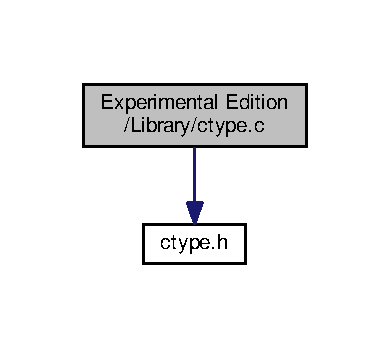
\includegraphics[width=187pt]{ctype_8c__incl}
\end{center}
\end{figure}
\subsection*{Functions}
\begin{DoxyCompactItemize}
\item 
char \hyperlink{ctype_8c_ae5f6cee1721ab27fffcbd8cd09e2238a}{toupper} (char a)
\item 
char \hyperlink{ctype_8c_a8aeccdcaa487c54b4b132734c70853f5}{tolower} (char a)
\end{DoxyCompactItemize}


\subsection{Function Documentation}
\index{ctype.\+c@{ctype.\+c}!tolower@{tolower}}
\index{tolower@{tolower}!ctype.\+c@{ctype.\+c}}
\subsubsection[{\texorpdfstring{tolower(char a)}{tolower(char a)}}]{\setlength{\rightskip}{0pt plus 5cm}char tolower (
\begin{DoxyParamCaption}
\item[{char}]{a}
\end{DoxyParamCaption}
)}\hypertarget{ctype_8c_a8aeccdcaa487c54b4b132734c70853f5}{}\label{ctype_8c_a8aeccdcaa487c54b4b132734c70853f5}


Definition at line 9 of file ctype.\+c.


\begin{DoxyCode}
10 \{
11     \textcolor{keywordflow}{if}(a>=65&&a<=91)
12         \textcolor{keywordflow}{return} a+32;
13     \textcolor{keywordflow}{else} \textcolor{keywordflow}{return} a;
14 \}
\end{DoxyCode}
\index{ctype.\+c@{ctype.\+c}!toupper@{toupper}}
\index{toupper@{toupper}!ctype.\+c@{ctype.\+c}}
\subsubsection[{\texorpdfstring{toupper(char a)}{toupper(char a)}}]{\setlength{\rightskip}{0pt plus 5cm}char toupper (
\begin{DoxyParamCaption}
\item[{char}]{a}
\end{DoxyParamCaption}
)}\hypertarget{ctype_8c_ae5f6cee1721ab27fffcbd8cd09e2238a}{}\label{ctype_8c_ae5f6cee1721ab27fffcbd8cd09e2238a}


Definition at line 3 of file ctype.\+c.


\begin{DoxyCode}
4 \{
5     \textcolor{keywordflow}{if}(a>=97&&a<=122)
6         \textcolor{keywordflow}{return} a-32;
7     \textcolor{keywordflow}{else} \textcolor{keywordflow}{return} a;
8 \}
\end{DoxyCode}

\hypertarget{ctype_8h}{}\section{Experimental Edition/\+Library/ctype.h File Reference}
\label{ctype_8h}\index{Experimental Edition/\+Library/ctype.\+h@{Experimental Edition/\+Library/ctype.\+h}}
This graph shows which files directly or indirectly include this file\+:
\nopagebreak
\begin{figure}[H]
\begin{center}
\leavevmode
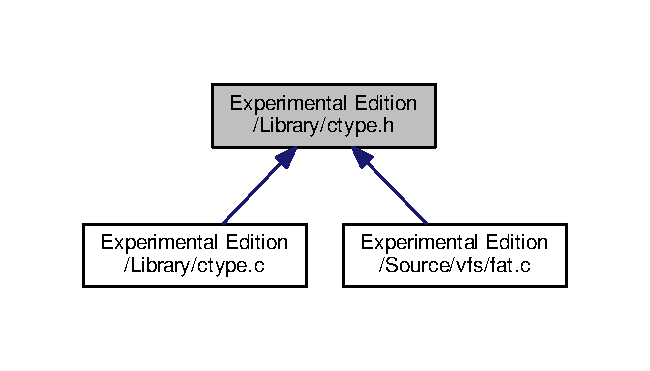
\includegraphics[width=312pt]{ctype_8h__dep__incl}
\end{center}
\end{figure}
\subsection*{Functions}
\begin{DoxyCompactItemize}
\item 
char \hyperlink{ctype_8h_ae5f6cee1721ab27fffcbd8cd09e2238a}{toupper} (char a)
\item 
char \hyperlink{ctype_8h_a8aeccdcaa487c54b4b132734c70853f5}{tolower} (char a)
\end{DoxyCompactItemize}


\subsection{Function Documentation}
\index{ctype.\+h@{ctype.\+h}!tolower@{tolower}}
\index{tolower@{tolower}!ctype.\+h@{ctype.\+h}}
\subsubsection[{\texorpdfstring{tolower(char a)}{tolower(char a)}}]{\setlength{\rightskip}{0pt plus 5cm}char tolower (
\begin{DoxyParamCaption}
\item[{char}]{a}
\end{DoxyParamCaption}
)}\hypertarget{ctype_8h_a8aeccdcaa487c54b4b132734c70853f5}{}\label{ctype_8h_a8aeccdcaa487c54b4b132734c70853f5}


Definition at line 9 of file ctype.\+c.


\begin{DoxyCode}
10 \{
11     \textcolor{keywordflow}{if}(a>=65&&a<=91)
12         \textcolor{keywordflow}{return} a+32;
13     \textcolor{keywordflow}{else} \textcolor{keywordflow}{return} a;
14 \}
\end{DoxyCode}
\index{ctype.\+h@{ctype.\+h}!toupper@{toupper}}
\index{toupper@{toupper}!ctype.\+h@{ctype.\+h}}
\subsubsection[{\texorpdfstring{toupper(char a)}{toupper(char a)}}]{\setlength{\rightskip}{0pt plus 5cm}char toupper (
\begin{DoxyParamCaption}
\item[{char}]{a}
\end{DoxyParamCaption}
)}\hypertarget{ctype_8h_ae5f6cee1721ab27fffcbd8cd09e2238a}{}\label{ctype_8h_ae5f6cee1721ab27fffcbd8cd09e2238a}


Definition at line 3 of file ctype.\+c.


\begin{DoxyCode}
4 \{
5     \textcolor{keywordflow}{if}(a>=97&&a<=122)
6         \textcolor{keywordflow}{return} a-32;
7     \textcolor{keywordflow}{else} \textcolor{keywordflow}{return} a;
8 \}
\end{DoxyCode}

\hypertarget{rand_8h}{}\section{Experimental Edition/\+Library/rand.h File Reference}
\label{rand_8h}\index{Experimental Edition/\+Library/rand.\+h@{Experimental Edition/\+Library/rand.\+h}}
{\ttfamily \#include \char`\"{}stdint-\/gcc.\+h\char`\"{}}\\*
{\ttfamily \#include \char`\"{}cmos.\+h\char`\"{}}\\*
Include dependency graph for rand.\+h\+:
\nopagebreak
\begin{figure}[H]
\begin{center}
\leavevmode
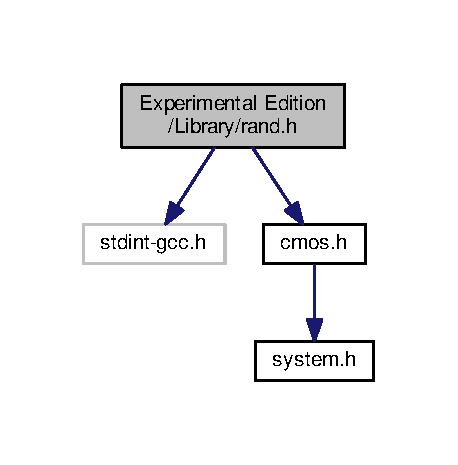
\includegraphics[width=220pt]{rand_8h__incl}
\end{center}
\end{figure}
This graph shows which files directly or indirectly include this file\+:
\nopagebreak
\begin{figure}[H]
\begin{center}
\leavevmode
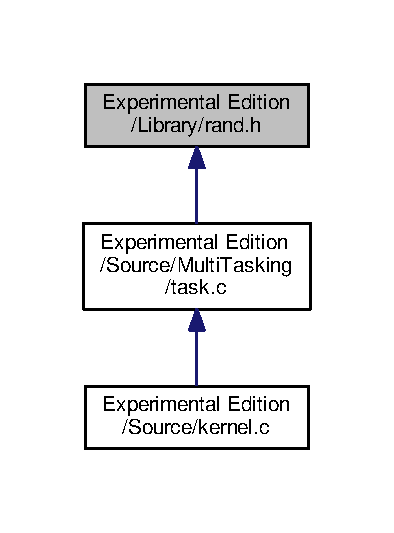
\includegraphics[width=189pt]{rand_8h__dep__incl}
\end{center}
\end{figure}
\subsection*{Functions}
\begin{DoxyCompactItemize}
\item 
int \hyperlink{rand_8h_a20e50ab9d6b10af0e2940d9419448f42}{rand} ()
\item 
void \hyperlink{rand_8h_a83a727cc697aea22e24cad5f39198dd2}{srand} (unsigned int seed)
\item 
void \hyperlink{rand_8h_ae21bf457e8314ad2bc3e8017121e4fe1}{srand\+Init} ()
\item 
int \hyperlink{rand_8h_a5548276cf6283fb605b1d869c6d05e37}{seeder} ()
\end{DoxyCompactItemize}
\subsection*{Variables}
\begin{DoxyCompactItemize}
\item 
volatile unsigned long int \hyperlink{rand_8h_a2d55800e2cf33074da1f8b53205c2619}{next} = 0
\item 
uint32\+\_\+t \hyperlink{rand_8h_ae73654f333e4363463ad8c594eca1905}{time}
\item 
uint32\+\_\+t \hyperlink{rand_8h_ab3507a48ae247ff252738ca350810b21}{ticks} =5
\end{DoxyCompactItemize}


\subsection{Function Documentation}
\index{rand.\+h@{rand.\+h}!rand@{rand}}
\index{rand@{rand}!rand.\+h@{rand.\+h}}
\subsubsection[{\texorpdfstring{rand()}{rand()}}]{\setlength{\rightskip}{0pt plus 5cm}int rand (
\begin{DoxyParamCaption}
{}
\end{DoxyParamCaption}
)\hspace{0.3cm}{\ttfamily [inline]}}\hypertarget{rand_8h_a20e50ab9d6b10af0e2940d9419448f42}{}\label{rand_8h_a20e50ab9d6b10af0e2940d9419448f42}


Definition at line 10 of file rand.\+h.


\begin{DoxyCode}
11 \{
12     \hyperlink{rand_8h_a2d55800e2cf33074da1f8b53205c2619}{next} = \hyperlink{rand_8h_a2d55800e2cf33074da1f8b53205c2619}{next} * 1103515245 + 12345;
13     \textcolor{keywordflow}{return} ((\hyperlink{rand_8h_a2d55800e2cf33074da1f8b53205c2619}{next} / 65536) % 32768);
14 \}
\end{DoxyCode}
\index{rand.\+h@{rand.\+h}!seeder@{seeder}}
\index{seeder@{seeder}!rand.\+h@{rand.\+h}}
\subsubsection[{\texorpdfstring{seeder()}{seeder()}}]{\setlength{\rightskip}{0pt plus 5cm}int seeder (
\begin{DoxyParamCaption}
{}
\end{DoxyParamCaption}
)}\hypertarget{rand_8h_a5548276cf6283fb605b1d869c6d05e37}{}\label{rand_8h_a5548276cf6283fb605b1d869c6d05e37}


Definition at line 28 of file rand.\+h.


\begin{DoxyCode}
29 \{
30     \textcolor{comment}{//rn=(int*)kmalloc(sizeof(int));}
31     \textcolor{keywordtype}{int} r=\hyperlink{rand_8h_a20e50ab9d6b10af0e2940d9419448f42}{rand}();
32    \textcolor{comment}{// r+=*rn;}
33    \textcolor{comment}{// kfree((void*)rn);}
34 
35     \textcolor{keywordflow}{return} r;
36 \}
\end{DoxyCode}


Here is the call graph for this function\+:
\nopagebreak
\begin{figure}[H]
\begin{center}
\leavevmode
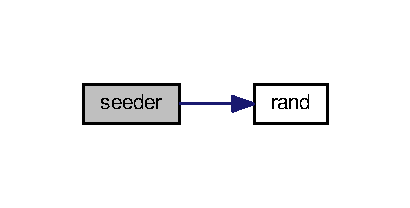
\includegraphics[width=197pt]{rand_8h_a5548276cf6283fb605b1d869c6d05e37_cgraph}
\end{center}
\end{figure}


\index{rand.\+h@{rand.\+h}!srand@{srand}}
\index{srand@{srand}!rand.\+h@{rand.\+h}}
\subsubsection[{\texorpdfstring{srand(unsigned int seed)}{srand(unsigned int seed)}}]{\setlength{\rightskip}{0pt plus 5cm}void srand (
\begin{DoxyParamCaption}
\item[{unsigned int}]{seed}
\end{DoxyParamCaption}
)\hspace{0.3cm}{\ttfamily [inline]}}\hypertarget{rand_8h_a83a727cc697aea22e24cad5f39198dd2}{}\label{rand_8h_a83a727cc697aea22e24cad5f39198dd2}


Definition at line 16 of file rand.\+h.


\begin{DoxyCode}
17 \{
18     \textcolor{comment}{//ticks=(next%5)+5;}
19     \hyperlink{rand_8h_a2d55800e2cf33074da1f8b53205c2619}{next} = (\hyperlink{rand_8h_a2d55800e2cf33074da1f8b53205c2619}{next}+seed)%100000;
20 \}
\end{DoxyCode}
\index{rand.\+h@{rand.\+h}!srand\+Init@{srand\+Init}}
\index{srand\+Init@{srand\+Init}!rand.\+h@{rand.\+h}}
\subsubsection[{\texorpdfstring{srand\+Init()}{srandInit()}}]{\setlength{\rightskip}{0pt plus 5cm}void srand\+Init (
\begin{DoxyParamCaption}
{}
\end{DoxyParamCaption}
)\hspace{0.3cm}{\ttfamily [inline]}}\hypertarget{rand_8h_ae21bf457e8314ad2bc3e8017121e4fe1}{}\label{rand_8h_ae21bf457e8314ad2bc3e8017121e4fe1}


Definition at line 22 of file rand.\+h.


\begin{DoxyCode}
23 \{
24     \hyperlink{rand_8h_ae73654f333e4363463ad8c594eca1905}{time}=\hyperlink{cmos_8c_ad86480bd4e099dc40dbbfc3ff58ede85}{ReadFromCMOS}();
25     \hyperlink{rand_8h_a83a727cc697aea22e24cad5f39198dd2}{srand}(\hyperlink{rand_8h_ae73654f333e4363463ad8c594eca1905}{time});
26 \}
\end{DoxyCode}


Here is the call graph for this function\+:
\nopagebreak
\begin{figure}[H]
\begin{center}
\leavevmode
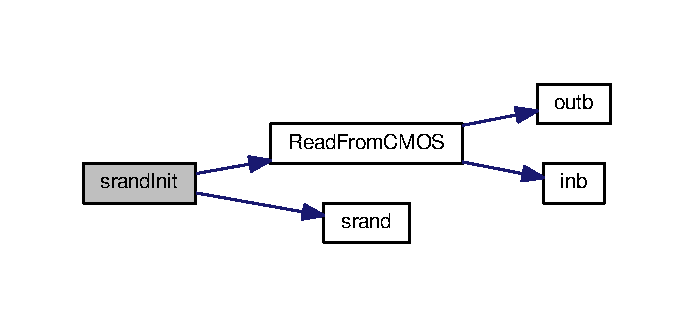
\includegraphics[width=333pt]{rand_8h_ae21bf457e8314ad2bc3e8017121e4fe1_cgraph}
\end{center}
\end{figure}




\subsection{Variable Documentation}
\index{rand.\+h@{rand.\+h}!next@{next}}
\index{next@{next}!rand.\+h@{rand.\+h}}
\subsubsection[{\texorpdfstring{next}{next}}]{\setlength{\rightskip}{0pt plus 5cm}volatile unsigned long int next = 0}\hypertarget{rand_8h_a2d55800e2cf33074da1f8b53205c2619}{}\label{rand_8h_a2d55800e2cf33074da1f8b53205c2619}


Definition at line 6 of file rand.\+h.

\index{rand.\+h@{rand.\+h}!ticks@{ticks}}
\index{ticks@{ticks}!rand.\+h@{rand.\+h}}
\subsubsection[{\texorpdfstring{ticks}{ticks}}]{\setlength{\rightskip}{0pt plus 5cm}uint32\+\_\+t ticks =5}\hypertarget{rand_8h_ab3507a48ae247ff252738ca350810b21}{}\label{rand_8h_ab3507a48ae247ff252738ca350810b21}


Definition at line 8 of file rand.\+h.

\index{rand.\+h@{rand.\+h}!time@{time}}
\index{time@{time}!rand.\+h@{rand.\+h}}
\subsubsection[{\texorpdfstring{time}{time}}]{\setlength{\rightskip}{0pt plus 5cm}uint32\+\_\+t time}\hypertarget{rand_8h_ae73654f333e4363463ad8c594eca1905}{}\label{rand_8h_ae73654f333e4363463ad8c594eca1905}


Definition at line 7 of file rand.\+h.


\hypertarget{stdio_8h}{}\section{Experimental Edition/\+Library/stdio.h File Reference}
\label{stdio_8h}\index{Experimental Edition/\+Library/stdio.\+h@{Experimental Edition/\+Library/stdio.\+h}}
{\ttfamily \#include $<$stdio.\+h$>$}\\*
{\ttfamily \#include $<$sys/cdefs.\+h$>$}\\*
{\ttfamily \#include $<$stdbool.\+h$>$}\\*
{\ttfamily \#include $<$stdarg.\+h$>$}\\*
{\ttfamily \#include $<$string.\+h$>$}\\*
Include dependency graph for stdio.\+h\+:
\nopagebreak
\begin{figure}[H]
\begin{center}
\leavevmode
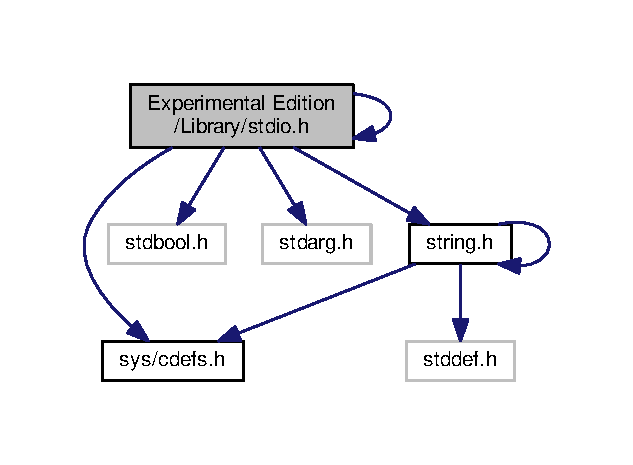
\includegraphics[width=304pt]{stdio_8h__incl}
\end{center}
\end{figure}
This graph shows which files directly or indirectly include this file\+:
\nopagebreak
\begin{figure}[H]
\begin{center}
\leavevmode
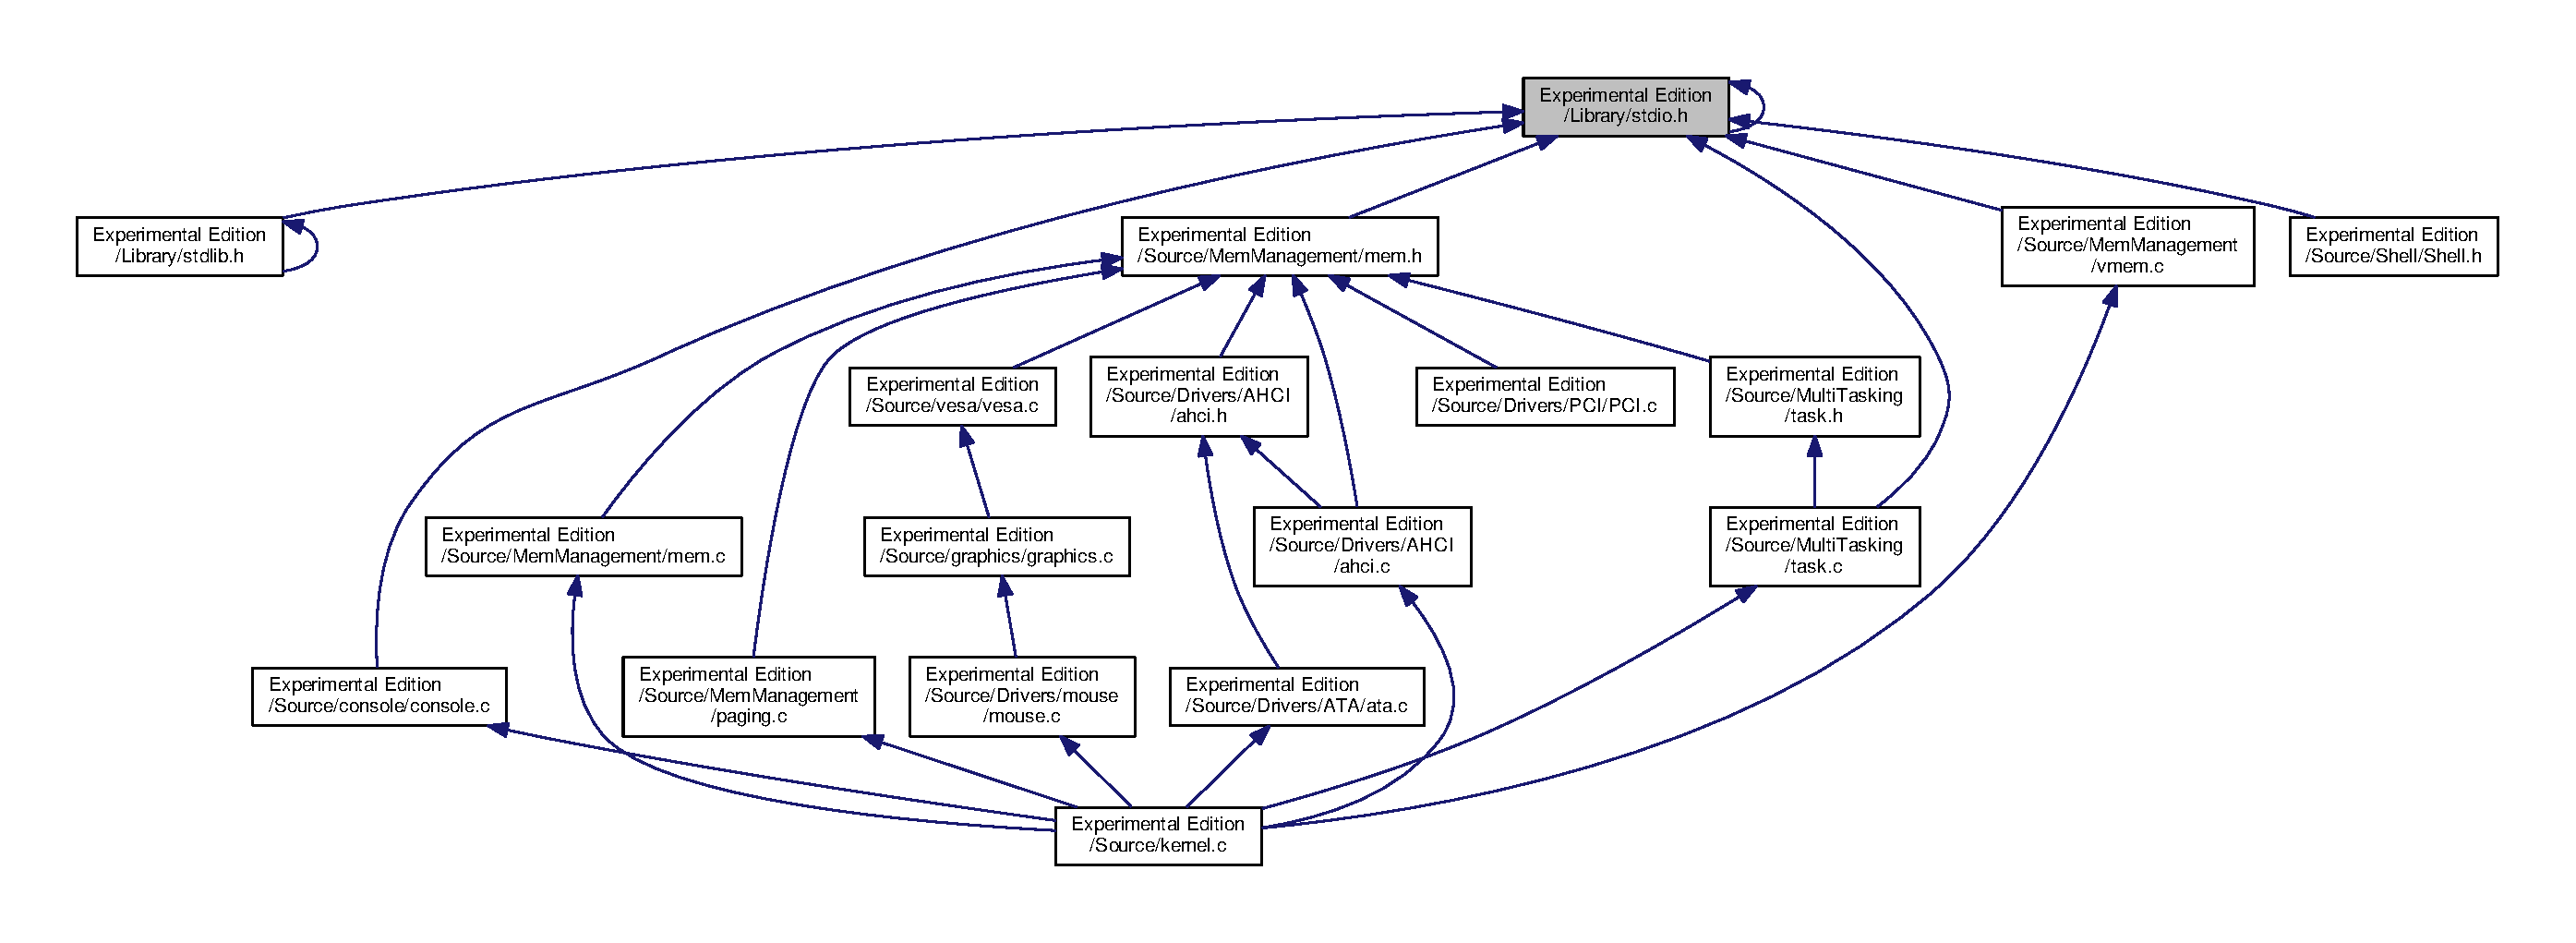
\includegraphics[width=350pt]{stdio_8h__dep__incl}
\end{center}
\end{figure}
\subsection*{Functions}
\begin{DoxyCompactItemize}
\item 
int \hyperlink{stdio_8h_ae8cb82b5dc7e5ff61f5610bdac37ff60}{putchar} (int ic)
\item 
void \hyperlink{stdio_8h_a4340730c5409b7e9981408c37974686d}{printint} (uint32\+\_\+t in)
\item 
int \hyperlink{stdio_8h_a9eff2528601a782ae056c1b1651bb5a8}{printf} (const char $\ast$restrict format,...)
\item 
void \hyperlink{stdio_8h_aa0f180d949f714d8235d398dd5fe0e34}{itoa} (unsigned i, unsigned \hyperlink{descriptors_8h_a0523cedff47e2441fc198b7770ec5d3f}{base}, char $\ast$buf)
\item 
int \hyperlink{stdio_8h_af17f2f3fda696ddc3b7c1bac995edaf8}{puts} (const char $\ast$string)
\end{DoxyCompactItemize}
\subsection*{Variables}
\begin{DoxyCompactItemize}
\item 
char \hyperlink{stdio_8h_ab54a389b6099ca9ceaf677e618ff584e}{tbuf} \mbox{[}32\mbox{]}
\item 
char \hyperlink{stdio_8h_ab3953c8d4a58fa01a96536ae63eb5e3e}{bchars} \mbox{[}$\,$\mbox{]} = \{\textquotesingle{}0\textquotesingle{},\textquotesingle{}1\textquotesingle{},\textquotesingle{}2\textquotesingle{},\textquotesingle{}3\textquotesingle{},\textquotesingle{}4\textquotesingle{},\textquotesingle{}5\textquotesingle{},\textquotesingle{}6\textquotesingle{},\textquotesingle{}7\textquotesingle{},\textquotesingle{}8\textquotesingle{},\textquotesingle{}9\textquotesingle{},\textquotesingle{}A\textquotesingle{},\textquotesingle{}B\textquotesingle{},\textquotesingle{}C\textquotesingle{},\textquotesingle{}D\textquotesingle{},\textquotesingle{}E\textquotesingle{},\textquotesingle{}F\textquotesingle{}\}
\end{DoxyCompactItemize}


\subsection{Function Documentation}
\index{stdio.\+h@{stdio.\+h}!itoa@{itoa}}
\index{itoa@{itoa}!stdio.\+h@{stdio.\+h}}
\subsubsection[{\texorpdfstring{itoa(unsigned i, unsigned base, char $\ast$buf)}{itoa(unsigned i, unsigned base, char *buf)}}]{\setlength{\rightskip}{0pt plus 5cm}void itoa (
\begin{DoxyParamCaption}
\item[{unsigned}]{i, }
\item[{unsigned}]{base, }
\item[{char $\ast$}]{buf}
\end{DoxyParamCaption}
)}\hypertarget{stdio_8h_aa0f180d949f714d8235d398dd5fe0e34}{}\label{stdio_8h_aa0f180d949f714d8235d398dd5fe0e34}


Definition at line 91 of file stdio.\+h.


\begin{DoxyCode}
91                                               \{
92    \textcolor{keywordtype}{int} pos = 0;
93    \textcolor{keywordtype}{int} opos = 0;
94    \textcolor{keywordtype}{int} top = 0;
95 
96    \textcolor{keywordflow}{if} (i == 0 || \hyperlink{descriptors_8h_a0523cedff47e2441fc198b7770ec5d3f}{base} > 16) \{
97       buf[0] = \textcolor{charliteral}{'0'};
98       buf[1] = \textcolor{charliteral}{'\(\backslash\)0'};
99       \textcolor{keywordflow}{return};
100    \}
101 
102    \textcolor{keywordflow}{while} (i != 0) \{
103       \hyperlink{stdio_8h_ab54a389b6099ca9ceaf677e618ff584e}{tbuf}[pos] = \hyperlink{stdio_8h_ab3953c8d4a58fa01a96536ae63eb5e3e}{bchars}[i % \hyperlink{descriptors_8h_a0523cedff47e2441fc198b7770ec5d3f}{base}];
104       pos++;
105       i /= \hyperlink{descriptors_8h_a0523cedff47e2441fc198b7770ec5d3f}{base};
106    \}
107    top=pos--;
108    \textcolor{keywordflow}{for} (opos=0; opos<top; pos--,opos++) \{
109       buf[opos] = \hyperlink{stdio_8h_ab54a389b6099ca9ceaf677e618ff584e}{tbuf}[pos];
110    \}
111    buf[opos] = 0;
112 \}
\end{DoxyCode}
\index{stdio.\+h@{stdio.\+h}!printf@{printf}}
\index{printf@{printf}!stdio.\+h@{stdio.\+h}}
\subsubsection[{\texorpdfstring{printf(const char $\ast$restrict format,...)}{printf(const char *restrict format,...)}}]{\setlength{\rightskip}{0pt plus 5cm}int printf (
\begin{DoxyParamCaption}
\item[{const char $\ast$restrict}]{format, }
\item[{}]{...}
\end{DoxyParamCaption}
)}\hypertarget{stdio_8h_a9eff2528601a782ae056c1b1651bb5a8}{}\label{stdio_8h_a9eff2528601a782ae056c1b1651bb5a8}


Definition at line 17 of file stdio.\+h.


\begin{DoxyCode}
18 \{
19     va\_list parameters;
20     va\_start(parameters, format);
21 
22     \textcolor{keywordtype}{int} written = 0;
23     \textcolor{keywordtype}{size\_t} amount;
24     \textcolor{keywordtype}{bool} rejected\_bad\_specifier = \textcolor{keyword}{false};
25 
26     \textcolor{keywordflow}{while} ( *format != \textcolor{charliteral}{'\(\backslash\)0'} )
27     \{
28         \textcolor{keywordflow}{if} ( *format != \textcolor{charliteral}{'%'} )
29         \{
30         print\_c:
31             amount = 1;
32             \textcolor{keywordflow}{while} ( format[amount] && format[amount] != \textcolor{charliteral}{'%'} )
33                 amount++;
34             print(format, amount);
35             format += amount;
36             written += amount;
37             \textcolor{keywordflow}{continue};
38         \}
39 
40         \textcolor{keyword}{const} \textcolor{keywordtype}{char}* format\_begun\_at = format;
41 
42         \textcolor{keywordflow}{if} ( *(++format) == \textcolor{charliteral}{'%'} )
43             \textcolor{keywordflow}{goto} print\_c;
44 
45         \textcolor{keywordflow}{if} ( rejected\_bad\_specifier )
46         \{
47         incomprehensible\_conversion:
48             rejected\_bad\_specifier = \textcolor{keyword}{true};
49             format = format\_begun\_at;
50             \textcolor{keywordflow}{goto} print\_c;
51         \}
52 
53         \textcolor{keywordflow}{if} ( *format == \textcolor{charliteral}{'c'} )
54         \{
55             format++;
56             \textcolor{keywordtype}{char} c = (char) va\_arg(parameters, \textcolor{keywordtype}{int} \textcolor{comment}{/* char promotes to int */});
57             print(&c, \textcolor{keyword}{sizeof}(c));
58         \}
59         \textcolor{keywordflow}{else} \textcolor{keywordflow}{if} ( *format == \textcolor{charliteral}{'s'} )
60         \{
61             format++;
62             \textcolor{keyword}{const} \textcolor{keywordtype}{char}* s = va\_arg(parameters, \textcolor{keyword}{const} \textcolor{keywordtype}{char}*);
63             print(s, \hyperlink{string_8h_a0e9d5be6802ed032f6354777ac0c1acf}{strlen}(s));
64         \}
65         \textcolor{keywordflow}{else} \textcolor{keywordflow}{if}(*format == \textcolor{charliteral}{'i'} ||*format == \textcolor{charliteral}{'d'})
66         \{
67             format++;
68             \textcolor{keywordtype}{int} c = va\_arg (parameters, \textcolor{keywordtype}{int});
69             \hyperlink{stdio_8h_a4340730c5409b7e9981408c37974686d}{printint}(c);
70         \}
71         \textcolor{keywordflow}{else} \textcolor{keywordflow}{if}(*format == \textcolor{charliteral}{'l'}||*format == \textcolor{charliteral}{'x'}) \textcolor{comment}{//uint32\_t}
72         \{
73             format++;
74             uint32\_t c = va\_arg (parameters, uint32\_t);
75             \hyperlink{stdio_8h_a4340730c5409b7e9981408c37974686d}{printint}(c);
76         \}
77         \textcolor{keywordflow}{else}
78         \{
79             \textcolor{keywordflow}{goto} incomprehensible\_conversion;
80         \}
81     \}
82 
83     va\_end(parameters);
84 
85     \textcolor{keywordflow}{return} written;
86 \}
\end{DoxyCode}


Here is the call graph for this function\+:
\nopagebreak
\begin{figure}[H]
\begin{center}
\leavevmode
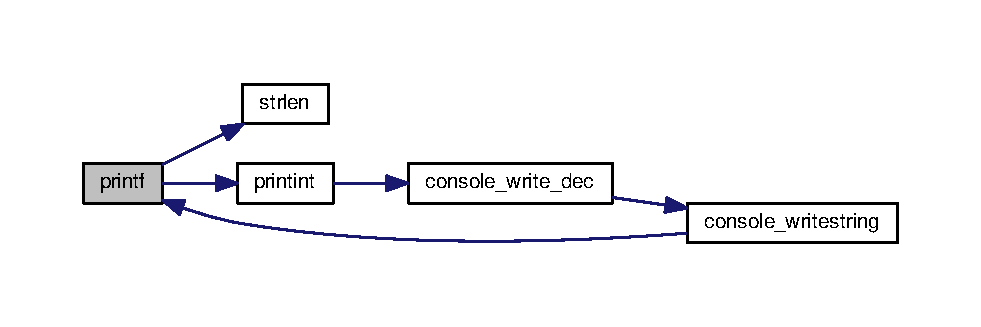
\includegraphics[width=350pt]{stdio_8h_a9eff2528601a782ae056c1b1651bb5a8_cgraph}
\end{center}
\end{figure}


\index{stdio.\+h@{stdio.\+h}!printint@{printint}}
\index{printint@{printint}!stdio.\+h@{stdio.\+h}}
\subsubsection[{\texorpdfstring{printint(uint32\+\_\+t in)}{printint(uint32_t in)}}]{\setlength{\rightskip}{0pt plus 5cm}void printint (
\begin{DoxyParamCaption}
\item[{uint32\+\_\+t}]{in}
\end{DoxyParamCaption}
)}\hypertarget{stdio_8h_a4340730c5409b7e9981408c37974686d}{}\label{stdio_8h_a4340730c5409b7e9981408c37974686d}


Definition at line 125 of file console.\+c.


\begin{DoxyCode}
126 \{
127     \textcolor{keywordflow}{if}(in<=999999999)
128         \hyperlink{console_8c_a0962a25f4eb04ccc0f0f2a1418091b35}{console\_write\_dec}(in);
129     \textcolor{keywordflow}{else}
130     \{
131         uint32\_t d=1,b=in,c=0;
132         \textcolor{keywordflow}{for}(uint32\_t i=0;b;i++)
133         \{
134             b=b/10;
135             ++c;
136         \}
137         c=c-9;
138         \textcolor{keywordflow}{for}(uint32\_t i=0;i<c;i++) d=d*10;
139         \hyperlink{console_8c_a0962a25f4eb04ccc0f0f2a1418091b35}{console\_write\_dec}(in/d);
140         \hyperlink{console_8c_a0962a25f4eb04ccc0f0f2a1418091b35}{console\_write\_dec}(in%d);
141     \}
142 \}
\end{DoxyCode}


Here is the call graph for this function\+:
\nopagebreak
\begin{figure}[H]
\begin{center}
\leavevmode
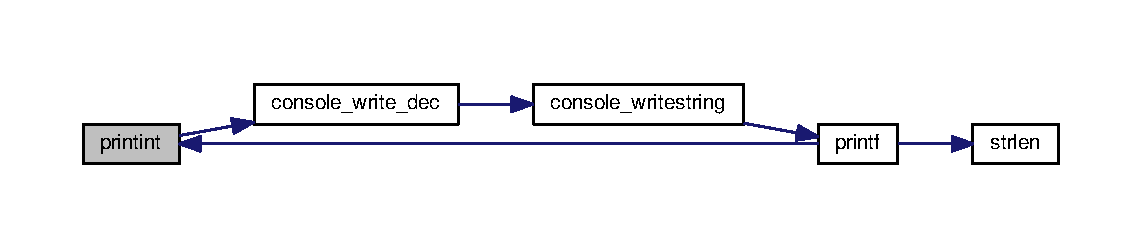
\includegraphics[width=350pt]{stdio_8h_a4340730c5409b7e9981408c37974686d_cgraph}
\end{center}
\end{figure}


\index{stdio.\+h@{stdio.\+h}!putchar@{putchar}}
\index{putchar@{putchar}!stdio.\+h@{stdio.\+h}}
\subsubsection[{\texorpdfstring{putchar(int ic)}{putchar(int ic)}}]{\setlength{\rightskip}{0pt plus 5cm}int putchar (
\begin{DoxyParamCaption}
\item[{int}]{ic}
\end{DoxyParamCaption}
)}\hypertarget{stdio_8h_ae8cb82b5dc7e5ff61f5610bdac37ff60}{}\label{stdio_8h_ae8cb82b5dc7e5ff61f5610bdac37ff60}


Definition at line 95 of file console.\+c.


\begin{DoxyCode}
96 \{
97     \textcolor{keywordtype}{char} c = (char) ic;
98     \hyperlink{console_8c_ad219d3a4d1adaa9323e5c3422f56f2ee}{console\_write}(&c, \textcolor{keyword}{sizeof}(c));
99     \textcolor{keywordflow}{return} ic;
100 \}
\end{DoxyCode}


Here is the call graph for this function\+:
\nopagebreak
\begin{figure}[H]
\begin{center}
\leavevmode
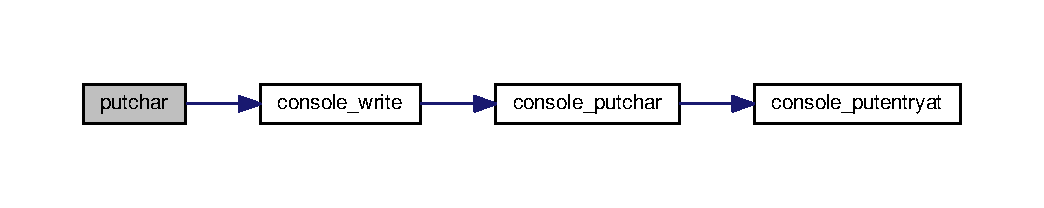
\includegraphics[width=350pt]{stdio_8h_ae8cb82b5dc7e5ff61f5610bdac37ff60_cgraph}
\end{center}
\end{figure}


\index{stdio.\+h@{stdio.\+h}!puts@{puts}}
\index{puts@{puts}!stdio.\+h@{stdio.\+h}}
\subsubsection[{\texorpdfstring{puts(const char $\ast$string)}{puts(const char *string)}}]{\setlength{\rightskip}{0pt plus 5cm}int puts (
\begin{DoxyParamCaption}
\item[{const char $\ast$}]{string}
\end{DoxyParamCaption}
)}\hypertarget{stdio_8h_af17f2f3fda696ddc3b7c1bac995edaf8}{}\label{stdio_8h_af17f2f3fda696ddc3b7c1bac995edaf8}


Definition at line 114 of file stdio.\+h.


\begin{DoxyCode}
115 \{
116     \textcolor{keywordflow}{return} \hyperlink{stdio_8h_a9eff2528601a782ae056c1b1651bb5a8}{printf}(\textcolor{stringliteral}{"%s\(\backslash\)n"}, \textcolor{keywordtype}{string});
117 \}
\end{DoxyCode}


Here is the call graph for this function\+:
\nopagebreak
\begin{figure}[H]
\begin{center}
\leavevmode
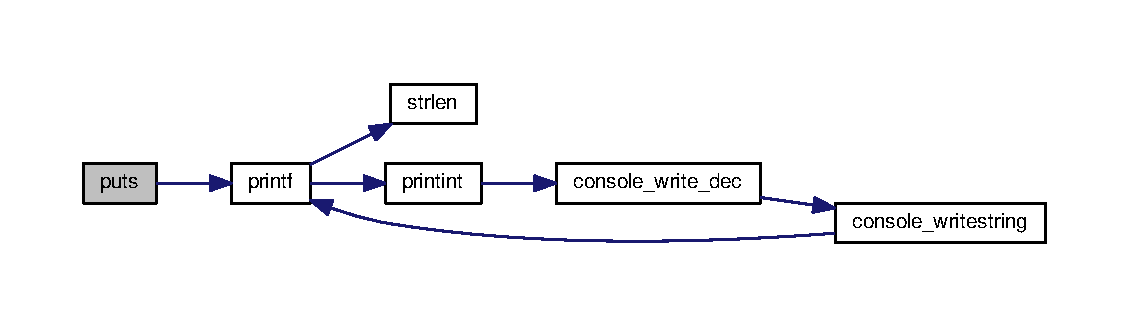
\includegraphics[width=350pt]{stdio_8h_af17f2f3fda696ddc3b7c1bac995edaf8_cgraph}
\end{center}
\end{figure}




\subsection{Variable Documentation}
\index{stdio.\+h@{stdio.\+h}!bchars@{bchars}}
\index{bchars@{bchars}!stdio.\+h@{stdio.\+h}}
\subsubsection[{\texorpdfstring{bchars}{bchars}}]{\setlength{\rightskip}{0pt plus 5cm}char bchars\mbox{[}$\,$\mbox{]} = \{\textquotesingle{}0\textquotesingle{},\textquotesingle{}1\textquotesingle{},\textquotesingle{}2\textquotesingle{},\textquotesingle{}3\textquotesingle{},\textquotesingle{}4\textquotesingle{},\textquotesingle{}5\textquotesingle{},\textquotesingle{}6\textquotesingle{},\textquotesingle{}7\textquotesingle{},\textquotesingle{}8\textquotesingle{},\textquotesingle{}9\textquotesingle{},\textquotesingle{}A\textquotesingle{},\textquotesingle{}B\textquotesingle{},\textquotesingle{}C\textquotesingle{},\textquotesingle{}D\textquotesingle{},\textquotesingle{}E\textquotesingle{},\textquotesingle{}F\textquotesingle{}\}}\hypertarget{stdio_8h_ab3953c8d4a58fa01a96536ae63eb5e3e}{}\label{stdio_8h_ab3953c8d4a58fa01a96536ae63eb5e3e}


Definition at line 89 of file stdio.\+h.

\index{stdio.\+h@{stdio.\+h}!tbuf@{tbuf}}
\index{tbuf@{tbuf}!stdio.\+h@{stdio.\+h}}
\subsubsection[{\texorpdfstring{tbuf}{tbuf}}]{\setlength{\rightskip}{0pt plus 5cm}char tbuf\mbox{[}32\mbox{]}}\hypertarget{stdio_8h_ab54a389b6099ca9ceaf677e618ff584e}{}\label{stdio_8h_ab54a389b6099ca9ceaf677e618ff584e}


Definition at line 88 of file stdio.\+h.


\hypertarget{stdlib_8h}{}\section{Experimental Edition/\+Library/stdlib.h File Reference}
\label{stdlib_8h}\index{Experimental Edition/\+Library/stdlib.\+h@{Experimental Edition/\+Library/stdlib.\+h}}
{\ttfamily \#include $<$stdlib.\+h$>$}\\*
{\ttfamily \#include $<$stdio.\+h$>$}\\*
Include dependency graph for stdlib.\+h\+:
\nopagebreak
\begin{figure}[H]
\begin{center}
\leavevmode
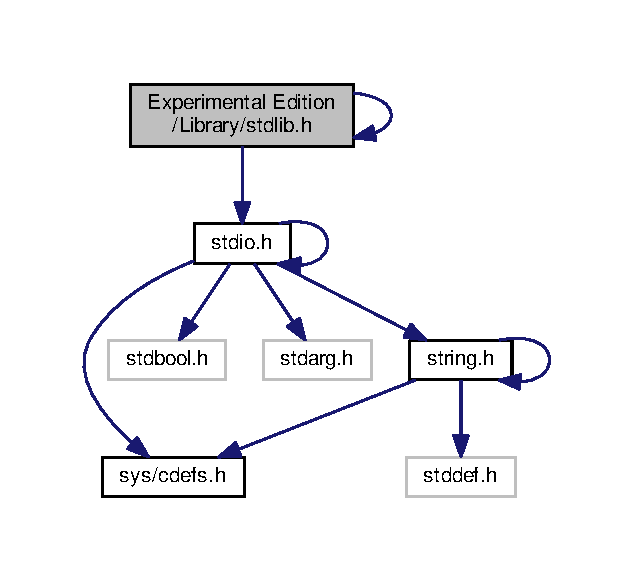
\includegraphics[width=304pt]{stdlib_8h__incl}
\end{center}
\end{figure}
This graph shows which files directly or indirectly include this file\+:
\nopagebreak
\begin{figure}[H]
\begin{center}
\leavevmode
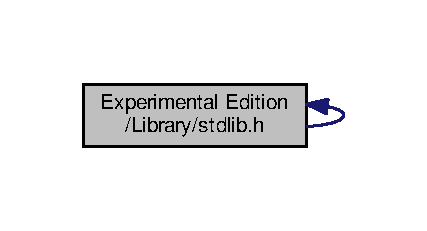
\includegraphics[width=205pt]{stdlib_8h__dep__incl}
\end{center}
\end{figure}
\subsection*{Functions}
\begin{DoxyCompactItemize}
\item 
\hyperlink{stdlib_8h_a342b9cd31607a848b169a5dcca6cc149}{\+\_\+\+\_\+attribute\+\_\+\+\_\+} ((\+\_\+\+\_\+noreturn\+\_\+\+\_\+)) void abort(void)
\end{DoxyCompactItemize}


\subsection{Function Documentation}
\index{stdlib.\+h@{stdlib.\+h}!\+\_\+\+\_\+attribute\+\_\+\+\_\+@{\+\_\+\+\_\+attribute\+\_\+\+\_\+}}
\index{\+\_\+\+\_\+attribute\+\_\+\+\_\+@{\+\_\+\+\_\+attribute\+\_\+\+\_\+}!stdlib.\+h@{stdlib.\+h}}
\subsubsection[{\texorpdfstring{\+\_\+\+\_\+attribute\+\_\+\+\_\+((\+\_\+\+\_\+noreturn\+\_\+\+\_\+)) void abort(void)}{__attribute__((__noreturn__)) void abort(void)}}]{\setlength{\rightskip}{0pt plus 5cm}{\bf \+\_\+\+\_\+attribute\+\_\+\+\_\+} (
\begin{DoxyParamCaption}
\item[{(\+\_\+\+\_\+noreturn\+\_\+\+\_\+)}]{}
\end{DoxyParamCaption}
)}\hypertarget{stdlib_8h_a342b9cd31607a848b169a5dcca6cc149}{}\label{stdlib_8h_a342b9cd31607a848b169a5dcca6cc149}


Definition at line 5 of file stdlib.\+h.


\begin{DoxyCode}
7 \{
8     \textcolor{comment}{// TODO: Add proper kernel panic.}
9     \hyperlink{stdio_8h_a9eff2528601a782ae056c1b1651bb5a8}{printf}(\textcolor{stringliteral}{"Kernel Panic: abort()\(\backslash\)n"});
10     \textcolor{keywordflow}{while} ( 1 ) \{ \}
11     \_\_builtin\_unreachable();
12 \}
\end{DoxyCode}


Here is the call graph for this function\+:
\nopagebreak
\begin{figure}[H]
\begin{center}
\leavevmode
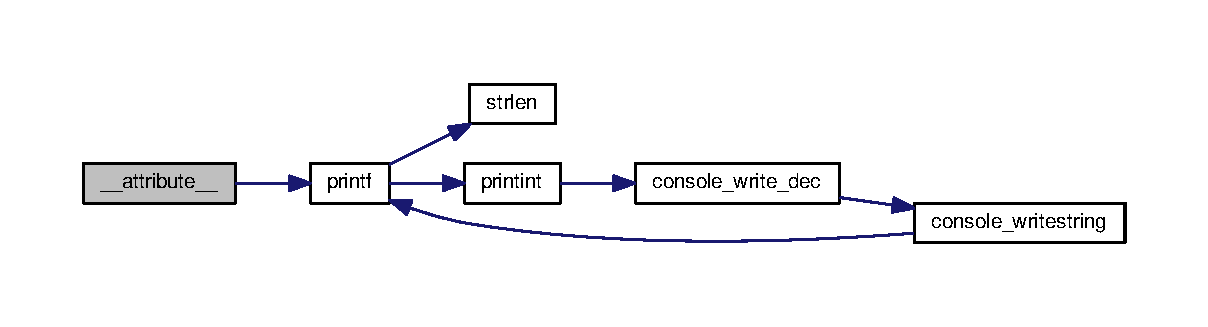
\includegraphics[width=350pt]{stdlib_8h_a342b9cd31607a848b169a5dcca6cc149_cgraph}
\end{center}
\end{figure}



\hypertarget{string_8h}{}\section{Experimental Edition/\+Library/string.h File Reference}
\label{string_8h}\index{Experimental Edition/\+Library/string.\+h@{Experimental Edition/\+Library/string.\+h}}
{\ttfamily \#include $<$string.\+h$>$}\\*
{\ttfamily \#include $<$sys/cdefs.\+h$>$}\\*
{\ttfamily \#include $<$stddef.\+h$>$}\\*
Include dependency graph for string.\+h\+:
\nopagebreak
\begin{figure}[H]
\begin{center}
\leavevmode
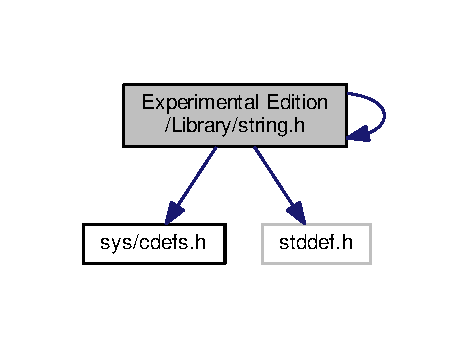
\includegraphics[width=225pt]{string_8h__incl}
\end{center}
\end{figure}
This graph shows which files directly or indirectly include this file\+:
\nopagebreak
\begin{figure}[H]
\begin{center}
\leavevmode
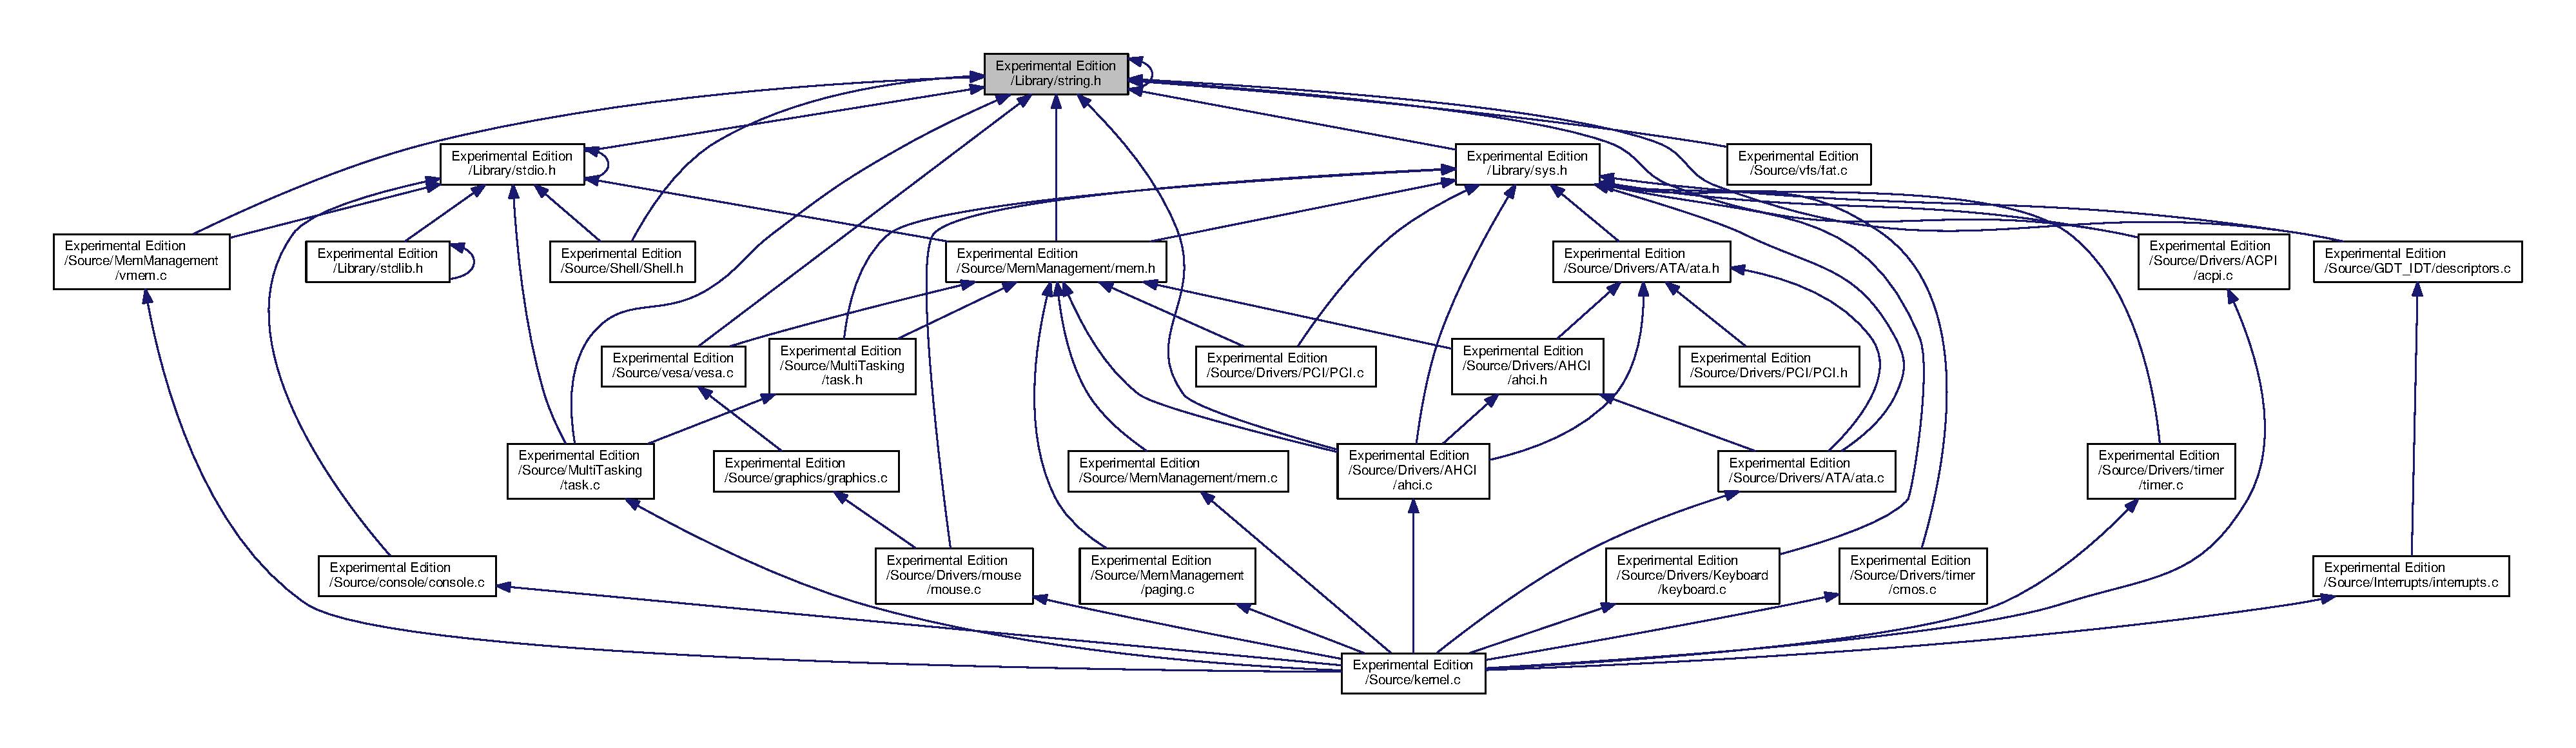
\includegraphics[width=350pt]{string_8h__dep__incl}
\end{center}
\end{figure}
\subsection*{Functions}
\begin{DoxyCompactItemize}
\item 
int \hyperlink{string_8h_a3376078c105a2293e911a180e7fbab4b}{memcmp} (const void $\ast$\+\_\+s1, const void $\ast$\+\_\+s2, size\+\_\+t \+\_\+n)
\item 
void $\ast$ \hyperlink{string_8h_a776fdd36ddff3e9f4191ea47e0cbd5de}{memcpy} (void $\ast$\+\_\+dest, const void $\ast$\+\_\+src, size\+\_\+t \+\_\+n)
\item 
void $\ast$ \hyperlink{string_8h_ae972269902c41dcc0afca72fc22af95f}{memmove} (void $\ast$dstptr, const void $\ast$srcptr, size\+\_\+t \hyperlink{multiboot_8h_a8c5ccb4d457cb24df33a7c9facfa2650}{size})
\item 
void \hyperlink{string_8h_ab70ae7ba054fd55023ccf5b7ceae875a}{memset} (void $\ast$\+\_\+s, int \+\_\+c, size\+\_\+t \+\_\+n)
\item 
size\+\_\+t \hyperlink{string_8h_a0e9d5be6802ed032f6354777ac0c1acf}{strlen} (const char $\ast$\+\_\+s)
\item 
int \hyperlink{string_8h_a34624c3be7459f677d90ae0ad046821a}{strcmp} (const char $\ast$\+\_\+s1, const char $\ast$\+\_\+s2)
\item 
int \hyperlink{string_8h_a7377c7836651b9c210e431b531ede0c8}{strncmp} (const char $\ast$\+\_\+s1, const char $\ast$\+\_\+s2, size\+\_\+t \+\_\+n)
\item 
char $\ast$ \hyperlink{string_8h_a5d193b0ce634c4a4915378441a475c46}{strcpy} (char $\ast$\+\_\+dest, const char $\ast$\+\_\+src)
\item 
char $\ast$ \hyperlink{string_8h_a98218333c64beb42f1b1d06da7d53329}{strcat} (char $\ast$\+\_\+dest, const char $\ast$\+\_\+src)
\item 
int \hyperlink{string_8h_a3487905a0eeaa950e7fedeed68ff9bf8}{strcmpy} (const char $\ast$c1, const char $\ast$c2)
\item 
char $\ast$ \hyperlink{string_8h_a0d822829769975a03cfc4b9b2bc83895}{strchr} (const char $\ast$\+\_\+s, int \+\_\+c)
\item 
size\+\_\+t \hyperlink{string_8h_a70edc6f218324e3355a0ad188ec84944}{strspn} (const char $\ast$\+\_\+s, const char $\ast$\+\_\+accept)
\item 
size\+\_\+t \hyperlink{string_8h_a9f9d868422cf96200bc5420a197895e6}{strcspn} (const char $\ast$\+\_\+s, const char $\ast$\+\_\+reject)
\item 
char $\ast$ \hyperlink{string_8h_ad1fc4977575eda6fb175df488baf3284}{strtok} (char $\ast$\+\_\+s, const char $\ast$\+\_\+delim)
\item 
char $\ast$ \hyperlink{string_8h_a0b12094c3530d2c7ba3bddde57520819}{strstr} (const char $\ast$\+\_\+haystack, const char $\ast$\+\_\+needle)
\end{DoxyCompactItemize}


\subsection{Function Documentation}
\index{string.\+h@{string.\+h}!memcmp@{memcmp}}
\index{memcmp@{memcmp}!string.\+h@{string.\+h}}
\subsubsection[{\texorpdfstring{memcmp(const void $\ast$\+\_\+s1, const void $\ast$\+\_\+s2, size\+\_\+t \+\_\+n)}{memcmp(const void *_s1, const void *_s2, size_t _n)}}]{\setlength{\rightskip}{0pt plus 5cm}int memcmp (
\begin{DoxyParamCaption}
\item[{const void $\ast$}]{\+\_\+s1, }
\item[{const void $\ast$}]{\+\_\+s2, }
\item[{size\+\_\+t}]{\+\_\+n}
\end{DoxyParamCaption}
)}\hypertarget{string_8h_a3376078c105a2293e911a180e7fbab4b}{}\label{string_8h_a3376078c105a2293e911a180e7fbab4b}


Definition at line 8 of file string.\+h.


\begin{DoxyCode}
9 \{
10     \textcolor{keyword}{const} \textcolor{keywordtype}{unsigned} \textcolor{keywordtype}{char} *us1 = (\textcolor{keyword}{const} \textcolor{keywordtype}{unsigned} \textcolor{keywordtype}{char} *)\_s1;
11     \textcolor{keyword}{const} \textcolor{keywordtype}{unsigned} \textcolor{keywordtype}{char} *us2 = (\textcolor{keyword}{const} \textcolor{keywordtype}{unsigned} \textcolor{keywordtype}{char} *)\_s2;
12     \textcolor{keywordflow}{while}(\_n-- != 0) \{
13         \textcolor{keywordflow}{if}(*us1 != *us2)\{
14             \textcolor{keywordflow}{return} (*us1 < *us2) ? -1 : +1;
15         \}
16         us1++;
17         us2++;
18     \}
19     \textcolor{keywordflow}{return} 0;
20 \}
\end{DoxyCode}
\index{string.\+h@{string.\+h}!memcpy@{memcpy}}
\index{memcpy@{memcpy}!string.\+h@{string.\+h}}
\subsubsection[{\texorpdfstring{memcpy(void $\ast$\+\_\+dest, const void $\ast$\+\_\+src, size\+\_\+t \+\_\+n)}{memcpy(void *_dest, const void *_src, size_t _n)}}]{\setlength{\rightskip}{0pt plus 5cm}void$\ast$ memcpy (
\begin{DoxyParamCaption}
\item[{void $\ast$}]{\+\_\+dest, }
\item[{const void $\ast$}]{\+\_\+src, }
\item[{size\+\_\+t}]{\+\_\+n}
\end{DoxyParamCaption}
)\hspace{0.3cm}{\ttfamily [inline]}}\hypertarget{string_8h_a776fdd36ddff3e9f4191ea47e0cbd5de}{}\label{string_8h_a776fdd36ddff3e9f4191ea47e0cbd5de}


Definition at line 22 of file string.\+h.


\begin{DoxyCode}
23 \{
24     \textcolor{keywordtype}{char} *sp = (\textcolor{keywordtype}{char}*) \_src;
25     \textcolor{keywordtype}{char} *dp = (\textcolor{keywordtype}{char}*) \_dest;
26     \textcolor{keywordflow}{for}(; \_n != 0; \_n--) \{
27         *dp++ = *sp++;
28     \}
29     \textcolor{keywordflow}{return} \_dest;
30 \}
\end{DoxyCode}
\index{string.\+h@{string.\+h}!memmove@{memmove}}
\index{memmove@{memmove}!string.\+h@{string.\+h}}
\subsubsection[{\texorpdfstring{memmove(void $\ast$dstptr, const void $\ast$srcptr, size\+\_\+t size)}{memmove(void *dstptr, const void *srcptr, size_t size)}}]{\setlength{\rightskip}{0pt plus 5cm}void$\ast$ memmove (
\begin{DoxyParamCaption}
\item[{void $\ast$}]{dstptr, }
\item[{const void $\ast$}]{srcptr, }
\item[{size\+\_\+t}]{size}
\end{DoxyParamCaption}
)}\hypertarget{string_8h_ae972269902c41dcc0afca72fc22af95f}{}\label{string_8h_ae972269902c41dcc0afca72fc22af95f}


Definition at line 32 of file string.\+h.


\begin{DoxyCode}
33 \{
34     \textcolor{keywordtype}{unsigned} \textcolor{keywordtype}{char}* dst = (\textcolor{keywordtype}{unsigned} \textcolor{keywordtype}{char}*) dstptr;
35     \textcolor{keyword}{const} \textcolor{keywordtype}{unsigned} \textcolor{keywordtype}{char}* src = (\textcolor{keyword}{const} \textcolor{keywordtype}{unsigned} \textcolor{keywordtype}{char}*) srcptr;
36     \textcolor{keywordflow}{if} ( dst < src )
37         \textcolor{keywordflow}{for} ( \textcolor{keywordtype}{size\_t} i = 0; i < \hyperlink{multiboot_8h_a8c5ccb4d457cb24df33a7c9facfa2650}{size}; i++ )
38             dst[i] = src[i];
39     \textcolor{keywordflow}{else}
40         \textcolor{keywordflow}{for} ( \textcolor{keywordtype}{size\_t} i = size; i != 0; i-- )
41             dst[i-1] = src[i-1];
42     \textcolor{keywordflow}{return} dstptr;
43 \}
\end{DoxyCode}
\index{string.\+h@{string.\+h}!memset@{memset}}
\index{memset@{memset}!string.\+h@{string.\+h}}
\subsubsection[{\texorpdfstring{memset(void $\ast$\+\_\+s, int \+\_\+c, size\+\_\+t \+\_\+n)}{memset(void *_s, int _c, size_t _n)}}]{\setlength{\rightskip}{0pt plus 5cm}void memset (
\begin{DoxyParamCaption}
\item[{void $\ast$}]{\+\_\+s, }
\item[{int}]{\+\_\+c, }
\item[{size\+\_\+t}]{\+\_\+n}
\end{DoxyParamCaption}
)}\hypertarget{string_8h_ab70ae7ba054fd55023ccf5b7ceae875a}{}\label{string_8h_ab70ae7ba054fd55023ccf5b7ceae875a}


Definition at line 46 of file string.\+h.


\begin{DoxyCode}
47 \{
48     \textcolor{keywordtype}{char} *temp = (\textcolor{keywordtype}{char}*) \_s;
49     \textcolor{keywordflow}{for} ( ; \_n != 0; \_n--) \{
50         *temp++ = \_c;
51     \}
52 \}
\end{DoxyCode}
\index{string.\+h@{string.\+h}!strcat@{strcat}}
\index{strcat@{strcat}!string.\+h@{string.\+h}}
\subsubsection[{\texorpdfstring{strcat(char $\ast$\+\_\+dest, const char $\ast$\+\_\+src)}{strcat(char *_dest, const char *_src)}}]{\setlength{\rightskip}{0pt plus 5cm}char$\ast$ strcat (
\begin{DoxyParamCaption}
\item[{char $\ast$}]{\+\_\+dest, }
\item[{const char $\ast$}]{\+\_\+src}
\end{DoxyParamCaption}
)}\hypertarget{string_8h_a98218333c64beb42f1b1d06da7d53329}{}\label{string_8h_a98218333c64beb42f1b1d06da7d53329}


Definition at line 98 of file string.\+h.


\begin{DoxyCode}
99 \{
100    \textcolor{keywordtype}{size\_t} n;
101 
102    n = \hyperlink{string_8h_a0e9d5be6802ed032f6354777ac0c1acf}{strlen}(\_dest);
103    \hyperlink{string_8h_a5d193b0ce634c4a4915378441a475c46}{strcpy}(\_dest + n, \_src);
104 
105    \textcolor{keywordflow}{return} \_dest;
106 \}
\end{DoxyCode}


Here is the call graph for this function\+:
\nopagebreak
\begin{figure}[H]
\begin{center}
\leavevmode
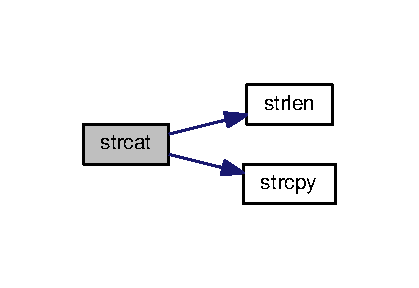
\includegraphics[width=201pt]{string_8h_a98218333c64beb42f1b1d06da7d53329_cgraph}
\end{center}
\end{figure}


\index{string.\+h@{string.\+h}!strchr@{strchr}}
\index{strchr@{strchr}!string.\+h@{string.\+h}}
\subsubsection[{\texorpdfstring{strchr(const char $\ast$\+\_\+s, int \+\_\+c)}{strchr(const char *_s, int _c)}}]{\setlength{\rightskip}{0pt plus 5cm}char$\ast$ strchr (
\begin{DoxyParamCaption}
\item[{const char $\ast$}]{\+\_\+s, }
\item[{int}]{\+\_\+c}
\end{DoxyParamCaption}
)}\hypertarget{string_8h_a0d822829769975a03cfc4b9b2bc83895}{}\label{string_8h_a0d822829769975a03cfc4b9b2bc83895}


Definition at line 127 of file string.\+h.


\begin{DoxyCode}
128 \{
129     \textcolor{keywordflow}{while} (*\_s != (\textcolor{keywordtype}{char})\_c) \{
130         \textcolor{keywordflow}{if} (!*\_s++) \{
131             \textcolor{keywordflow}{return} 0;
132         \}
133     \}
134     \textcolor{keywordflow}{return} (\textcolor{keywordtype}{char} *)\_s;
135 \}
\end{DoxyCode}
\index{string.\+h@{string.\+h}!strcmp@{strcmp}}
\index{strcmp@{strcmp}!string.\+h@{string.\+h}}
\subsubsection[{\texorpdfstring{strcmp(const char $\ast$\+\_\+s1, const char $\ast$\+\_\+s2)}{strcmp(const char *_s1, const char *_s2)}}]{\setlength{\rightskip}{0pt plus 5cm}int strcmp (
\begin{DoxyParamCaption}
\item[{const char $\ast$}]{\+\_\+s1, }
\item[{const char $\ast$}]{\+\_\+s2}
\end{DoxyParamCaption}
)}\hypertarget{string_8h_a34624c3be7459f677d90ae0ad046821a}{}\label{string_8h_a34624c3be7459f677d90ae0ad046821a}


Definition at line 63 of file string.\+h.


\begin{DoxyCode}
64 \{
65     \textcolor{keywordflow}{for}(; *\_s1 == *\_s2; ++\_s1, ++\_s2) \{
66         \textcolor{keywordflow}{if}(*\_s1 == 0) \{
67             \textcolor{keywordflow}{return} 0;
68         \}
69     \}
70     \textcolor{keywordflow}{return} *(\textcolor{keywordtype}{unsigned} \textcolor{keywordtype}{char} *)\_s1 < *(\textcolor{keywordtype}{unsigned} \textcolor{keywordtype}{char} *)\_s2 ? -1 : 1;
71 \}
\end{DoxyCode}
\index{string.\+h@{string.\+h}!strcmpy@{strcmpy}}
\index{strcmpy@{strcmpy}!string.\+h@{string.\+h}}
\subsubsection[{\texorpdfstring{strcmpy(const char $\ast$c1, const char $\ast$c2)}{strcmpy(const char *c1, const char *c2)}}]{\setlength{\rightskip}{0pt plus 5cm}int strcmpy (
\begin{DoxyParamCaption}
\item[{const char $\ast$}]{c1, }
\item[{const char $\ast$}]{c2}
\end{DoxyParamCaption}
)}\hypertarget{string_8h_a3487905a0eeaa950e7fedeed68ff9bf8}{}\label{string_8h_a3487905a0eeaa950e7fedeed68ff9bf8}


Definition at line 108 of file string.\+h.


\begin{DoxyCode}
109 \{
110     uint32\_t \hyperlink{vesa_8c_af30c10a8c6ed3d4649cfdc61e2029dc3}{buff}=0;
111     \textcolor{keywordflow}{for}(uint32\_t i=0;i<=\hyperlink{string_8h_a0e9d5be6802ed032f6354777ac0c1acf}{strlen}(c1);i++)
112     \{
113         \textcolor{keywordflow}{for}(uint32\_t j=0;j<\hyperlink{string_8h_a0e9d5be6802ed032f6354777ac0c1acf}{strlen}(c2);j++)
114         \{
115             \textcolor{keywordflow}{if}(c1[i+j]==c2[j])
116             \{
117                 buff+=1;
118             \}
119         \}
120         \textcolor{keywordflow}{if}(buff==\hyperlink{string_8h_a0e9d5be6802ed032f6354777ac0c1acf}{strlen}(c2))
121             \textcolor{keywordflow}{return} 0;
122         \textcolor{keywordflow}{else} buff=0;
123     \}
124     \textcolor{keywordflow}{return} 1;
125 \}
\end{DoxyCode}


Here is the call graph for this function\+:
\nopagebreak
\begin{figure}[H]
\begin{center}
\leavevmode
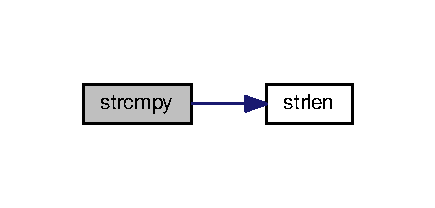
\includegraphics[width=209pt]{string_8h_a3487905a0eeaa950e7fedeed68ff9bf8_cgraph}
\end{center}
\end{figure}


\index{string.\+h@{string.\+h}!strcpy@{strcpy}}
\index{strcpy@{strcpy}!string.\+h@{string.\+h}}
\subsubsection[{\texorpdfstring{strcpy(char $\ast$\+\_\+dest, const char $\ast$\+\_\+src)}{strcpy(char *_dest, const char *_src)}}]{\setlength{\rightskip}{0pt plus 5cm}char$\ast$ strcpy (
\begin{DoxyParamCaption}
\item[{char $\ast$}]{\+\_\+dest, }
\item[{const char $\ast$}]{\+\_\+src}
\end{DoxyParamCaption}
)}\hypertarget{string_8h_a5d193b0ce634c4a4915378441a475c46}{}\label{string_8h_a5d193b0ce634c4a4915378441a475c46}


Definition at line 90 of file string.\+h.


\begin{DoxyCode}
91 \{
92     \textcolor{keywordflow}{do} \{
93       *\_dest++ = *\_src++;
94     \} \textcolor{keywordflow}{while} (*\_src != 0);
95     \textcolor{keywordflow}{return} \_dest;
96 \}
\end{DoxyCode}
\index{string.\+h@{string.\+h}!strcspn@{strcspn}}
\index{strcspn@{strcspn}!string.\+h@{string.\+h}}
\subsubsection[{\texorpdfstring{strcspn(const char $\ast$\+\_\+s, const char $\ast$\+\_\+reject)}{strcspn(const char *_s, const char *_reject)}}]{\setlength{\rightskip}{0pt plus 5cm}size\+\_\+t strcspn (
\begin{DoxyParamCaption}
\item[{const char $\ast$}]{\+\_\+s, }
\item[{const char $\ast$}]{\+\_\+reject}
\end{DoxyParamCaption}
)}\hypertarget{string_8h_a9f9d868422cf96200bc5420a197895e6}{}\label{string_8h_a9f9d868422cf96200bc5420a197895e6}


Definition at line 146 of file string.\+h.


\begin{DoxyCode}
147 \{
148     \textcolor{keywordtype}{size\_t} ret=0;
149     \textcolor{keywordflow}{while}(*\_s) \{
150         \textcolor{keywordflow}{if}(\hyperlink{string_8h_a0d822829769975a03cfc4b9b2bc83895}{strchr}(\_reject,*\_s)) \{
151             \textcolor{keywordflow}{return} ret;
152         \} \textcolor{keywordflow}{else} \{
153             \_s++,ret++;
154         \}
155     \}
156     \textcolor{keywordflow}{return} ret;
157 \}
\end{DoxyCode}


Here is the call graph for this function\+:
\nopagebreak
\begin{figure}[H]
\begin{center}
\leavevmode
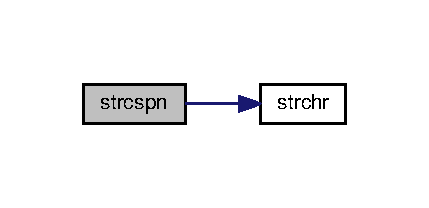
\includegraphics[width=206pt]{string_8h_a9f9d868422cf96200bc5420a197895e6_cgraph}
\end{center}
\end{figure}


\index{string.\+h@{string.\+h}!strlen@{strlen}}
\index{strlen@{strlen}!string.\+h@{string.\+h}}
\subsubsection[{\texorpdfstring{strlen(const char $\ast$\+\_\+s)}{strlen(const char *_s)}}]{\setlength{\rightskip}{0pt plus 5cm}size\+\_\+t strlen (
\begin{DoxyParamCaption}
\item[{const char $\ast$}]{\+\_\+s}
\end{DoxyParamCaption}
)}\hypertarget{string_8h_a0e9d5be6802ed032f6354777ac0c1acf}{}\label{string_8h_a0e9d5be6802ed032f6354777ac0c1acf}


Definition at line 54 of file string.\+h.


\begin{DoxyCode}
55 \{
56    \textcolor{keywordtype}{size\_t} n;
57    \textcolor{keywordflow}{for}(n=0; \_s[n] != \textcolor{charliteral}{'\(\backslash\)0'}; n++) \{
58        ;
59    \}
60    \textcolor{keywordflow}{return} n;
61 \}
\end{DoxyCode}
\index{string.\+h@{string.\+h}!strncmp@{strncmp}}
\index{strncmp@{strncmp}!string.\+h@{string.\+h}}
\subsubsection[{\texorpdfstring{strncmp(const char $\ast$\+\_\+s1, const char $\ast$\+\_\+s2, size\+\_\+t \+\_\+n)}{strncmp(const char *_s1, const char *_s2, size_t _n)}}]{\setlength{\rightskip}{0pt plus 5cm}int strncmp (
\begin{DoxyParamCaption}
\item[{const char $\ast$}]{\+\_\+s1, }
\item[{const char $\ast$}]{\+\_\+s2, }
\item[{size\+\_\+t}]{\+\_\+n}
\end{DoxyParamCaption}
)}\hypertarget{string_8h_a7377c7836651b9c210e431b531ede0c8}{}\label{string_8h_a7377c7836651b9c210e431b531ede0c8}


Definition at line 73 of file string.\+h.


\begin{DoxyCode}
74 \{
75     \textcolor{keywordtype}{unsigned} \textcolor{keywordtype}{char} uc1, uc2;
76     \textcolor{keywordflow}{if} (\_n==0)
77         \textcolor{keywordflow}{return} 0;
78     \textcolor{keywordflow}{while} (\_n-- > 0 && *\_s1 == *\_s2) \{
79         \textcolor{keywordflow}{if} (\_n==0 || *\_s1 == \textcolor{charliteral}{'\(\backslash\)0'} ) \{
80             \textcolor{keywordflow}{return} 0;
81         \}
82         \_s1++;
83         \_s2++;
84     \}
85     uc1 = (*(\textcolor{keywordtype}{unsigned} \textcolor{keywordtype}{char} *) \_s1);
86     uc2 = (*(\textcolor{keywordtype}{unsigned} \textcolor{keywordtype}{char} *) \_s2);
87     \textcolor{keywordflow}{return} ((uc1 < uc2) ? -1 : (uc1 > uc2));
88 \}
\end{DoxyCode}
\index{string.\+h@{string.\+h}!strspn@{strspn}}
\index{strspn@{strspn}!string.\+h@{string.\+h}}
\subsubsection[{\texorpdfstring{strspn(const char $\ast$\+\_\+s, const char $\ast$\+\_\+accept)}{strspn(const char *_s, const char *_accept)}}]{\setlength{\rightskip}{0pt plus 5cm}size\+\_\+t strspn (
\begin{DoxyParamCaption}
\item[{const char $\ast$}]{\+\_\+s, }
\item[{const char $\ast$}]{\+\_\+accept}
\end{DoxyParamCaption}
)}\hypertarget{string_8h_a70edc6f218324e3355a0ad188ec84944}{}\label{string_8h_a70edc6f218324e3355a0ad188ec84944}


Definition at line 137 of file string.\+h.


\begin{DoxyCode}
138 \{
139     \textcolor{keywordtype}{size\_t} ret=0;
140     \textcolor{keywordflow}{while}(*\_s && \hyperlink{string_8h_a0d822829769975a03cfc4b9b2bc83895}{strchr}(\_accept,*\_s++)) \{
141         ret++;
142     \}
143     \textcolor{keywordflow}{return} ret;
144 \}
\end{DoxyCode}


Here is the call graph for this function\+:
\nopagebreak
\begin{figure}[H]
\begin{center}
\leavevmode
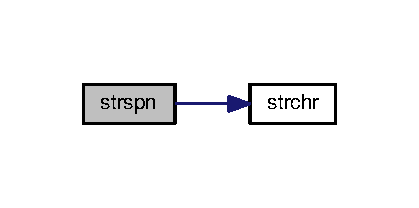
\includegraphics[width=201pt]{string_8h_a70edc6f218324e3355a0ad188ec84944_cgraph}
\end{center}
\end{figure}


\index{string.\+h@{string.\+h}!strstr@{strstr}}
\index{strstr@{strstr}!string.\+h@{string.\+h}}
\subsubsection[{\texorpdfstring{strstr(const char $\ast$\+\_\+haystack, const char $\ast$\+\_\+needle)}{strstr(const char *_haystack, const char *_needle)}}]{\setlength{\rightskip}{0pt plus 5cm}char$\ast$ strstr (
\begin{DoxyParamCaption}
\item[{const char $\ast$}]{\+\_\+haystack, }
\item[{const char $\ast$}]{\+\_\+needle}
\end{DoxyParamCaption}
)}\hypertarget{string_8h_a0b12094c3530d2c7ba3bddde57520819}{}\label{string_8h_a0b12094c3530d2c7ba3bddde57520819}


Definition at line 176 of file string.\+h.


\begin{DoxyCode}
177 \{
178     \textcolor{keywordtype}{size\_t} needleLen;
179     \textcolor{keywordflow}{if}(*\_needle == \textcolor{charliteral}{'\(\backslash\)0'}) \{
180         \textcolor{keywordflow}{return} (\textcolor{keywordtype}{char} *) \_haystack;
181     \}
182     needleLen = \hyperlink{string_8h_a0e9d5be6802ed032f6354777ac0c1acf}{strlen}(\_needle);
183 
184     \textcolor{keywordflow}{for}(;(\_haystack = \hyperlink{string_8h_a0d822829769975a03cfc4b9b2bc83895}{strchr}(\_haystack, *\_needle))!= \hyperlink{common_8h_a070d2ce7b6bb7e5c05602aa8c308d0c4}{NULL};\_haystack++) \{
185         \textcolor{keywordflow}{if} (\hyperlink{string_8h_a7377c7836651b9c210e431b531ede0c8}{strncmp}(\_haystack, \_needle, needleLen) == 0) \{
186             \textcolor{keywordflow}{return} (\textcolor{keywordtype}{char} *) \_haystack;
187         \}
188     \}
189     \textcolor{keywordflow}{return} \hyperlink{common_8h_a070d2ce7b6bb7e5c05602aa8c308d0c4}{NULL};
190 \}
\end{DoxyCode}


Here is the call graph for this function\+:
\nopagebreak
\begin{figure}[H]
\begin{center}
\leavevmode
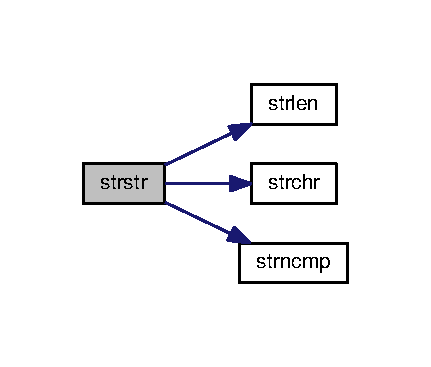
\includegraphics[width=207pt]{string_8h_a0b12094c3530d2c7ba3bddde57520819_cgraph}
\end{center}
\end{figure}


\index{string.\+h@{string.\+h}!strtok@{strtok}}
\index{strtok@{strtok}!string.\+h@{string.\+h}}
\subsubsection[{\texorpdfstring{strtok(char $\ast$\+\_\+s, const char $\ast$\+\_\+delim)}{strtok(char *_s, const char *_delim)}}]{\setlength{\rightskip}{0pt plus 5cm}char$\ast$ strtok (
\begin{DoxyParamCaption}
\item[{char $\ast$}]{\+\_\+s, }
\item[{const char $\ast$}]{\+\_\+delim}
\end{DoxyParamCaption}
)}\hypertarget{string_8h_ad1fc4977575eda6fb175df488baf3284}{}\label{string_8h_ad1fc4977575eda6fb175df488baf3284}


Definition at line 159 of file string.\+h.


\begin{DoxyCode}
160 \{
161     \textcolor{keyword}{static} \textcolor{keywordtype}{char}* p=0;
162     \textcolor{keywordflow}{if}(\_s) \{
163         p=\_s;
164     \} \textcolor{keywordflow}{else} \textcolor{keywordflow}{if}(!p) \{
165         \textcolor{keywordflow}{return} 0;
166     \}
167     \_s = p   + \hyperlink{string_8h_a70edc6f218324e3355a0ad188ec84944}{strspn}(p,\_delim);
168     p  = \_s  + \hyperlink{string_8h_a9f9d868422cf96200bc5420a197895e6}{strcspn}(\_s,\_delim);
169     \textcolor{keywordflow}{if}(p==\_s) \{
170         \textcolor{keywordflow}{return} p=0;
171     \}
172     p = *p ? *p=0,p+1 : 0;
173     \textcolor{keywordflow}{return} \_s;
174 \}
\end{DoxyCode}


Here is the call graph for this function\+:
\nopagebreak
\begin{figure}[H]
\begin{center}
\leavevmode
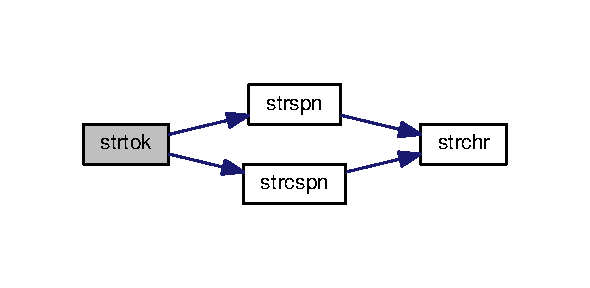
\includegraphics[width=283pt]{string_8h_ad1fc4977575eda6fb175df488baf3284_cgraph}
\end{center}
\end{figure}



\hypertarget{sys_8h}{}\section{Experimental Edition/\+Library/sys.h File Reference}
\label{sys_8h}\index{Experimental Edition/\+Library/sys.\+h@{Experimental Edition/\+Library/sys.\+h}}
{\ttfamily \#include $<$common.\+h$>$}\\*
{\ttfamily \#include $<$acpi.\+h$>$}\\*
{\ttfamily \#include $<$string.\+h$>$}\\*
Include dependency graph for sys.\+h\+:
\nopagebreak
\begin{figure}[H]
\begin{center}
\leavevmode
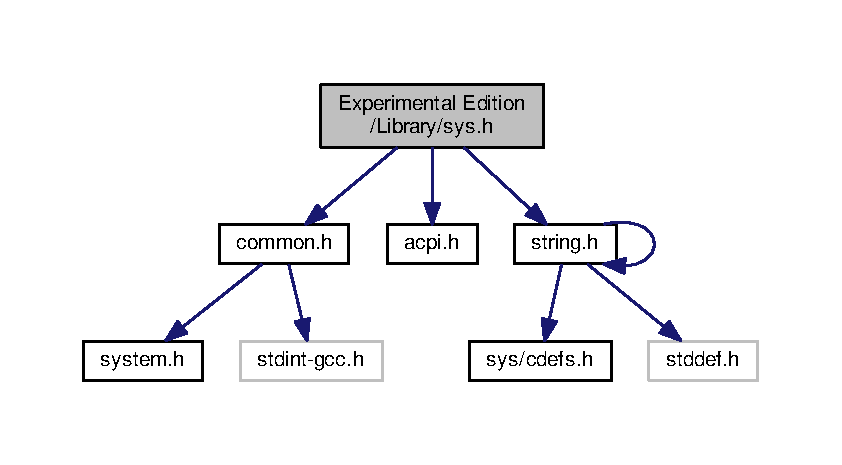
\includegraphics[width=350pt]{sys_8h__incl}
\end{center}
\end{figure}
This graph shows which files directly or indirectly include this file\+:
\nopagebreak
\begin{figure}[H]
\begin{center}
\leavevmode
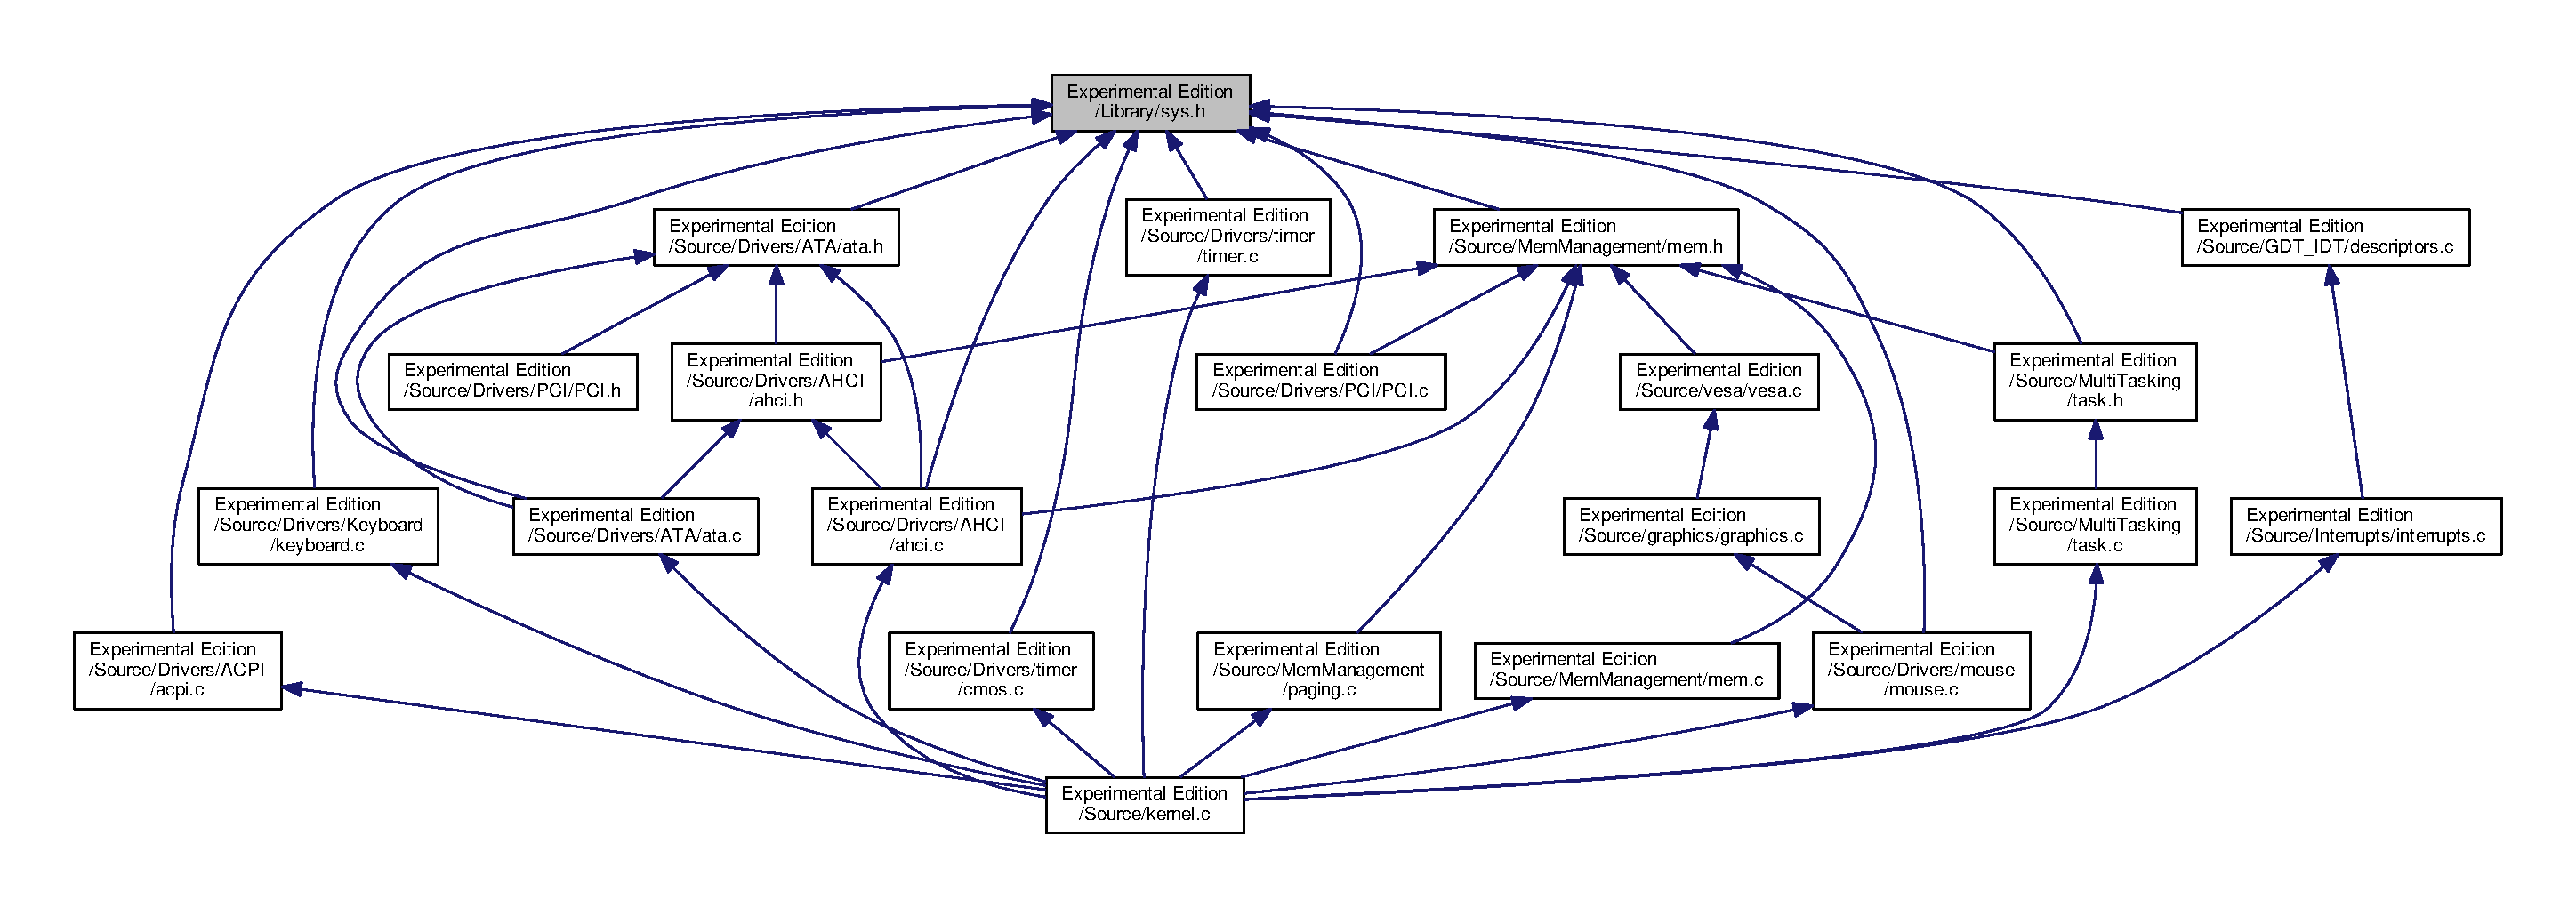
\includegraphics[width=350pt]{sys_8h__dep__incl}
\end{center}
\end{figure}
\subsection*{Functions}
\begin{DoxyCompactItemize}
\item 
void \hyperlink{sys_8h_ab08497f80e933a6a6171b89f1e524d37}{delay} (uint32\+\_\+t delay)
\item 
void \hyperlink{sys_8h_a1fe613f83e149aa1a4ae0d5f5149ab34}{outb} (\hyperlink{common_8h_ade81be9b965e7be1641f9792ba8af75e}{u16int} port, \hyperlink{common_8h_a27a416e6606c138f2d33233142a5593e}{u8int} val)
\item 
\hyperlink{common_8h_a27a416e6606c138f2d33233142a5593e}{u8int} \hyperlink{sys_8h_a3d758e66f0e4acaf38ba39b58ce83e4d}{inb} (\hyperlink{common_8h_ade81be9b965e7be1641f9792ba8af75e}{u16int} port)
\item 
void \hyperlink{sys_8h_aab8bf5abe19006ff9a80654d87f98908}{outw} (\hyperlink{common_8h_ade81be9b965e7be1641f9792ba8af75e}{u16int} port, \hyperlink{common_8h_ade81be9b965e7be1641f9792ba8af75e}{u16int} val)
\item 
\hyperlink{common_8h_ade81be9b965e7be1641f9792ba8af75e}{u16int} \hyperlink{sys_8h_a3dcbb9e13203beb0e38956999e8ae61d}{inw} (\hyperlink{common_8h_ade81be9b965e7be1641f9792ba8af75e}{u16int} port)
\item 
void \hyperlink{sys_8h_acc6d626f1f62f970a3c0ec95c09f7288}{outpd} (\hyperlink{common_8h_ade81be9b965e7be1641f9792ba8af75e}{u16int} port, \hyperlink{common_8h_ade81be9b965e7be1641f9792ba8af75e}{u16int} val)
\item 
\hyperlink{common_8h_ade81be9b965e7be1641f9792ba8af75e}{u16int} \hyperlink{sys_8h_a18bf8c1f3d6dcf4bc01a02224ee39668}{inpd} (\hyperlink{common_8h_ade81be9b965e7be1641f9792ba8af75e}{u16int} port)
\item 
void \hyperlink{sys_8h_ab53ee9eece30b2ac66ec33f66ebaa325}{outl} (\hyperlink{common_8h_ade81be9b965e7be1641f9792ba8af75e}{u16int} port, \hyperlink{common_8h_a7ae3a26c17ddfe117c6291739780801d}{u32int} val)
\item 
\hyperlink{common_8h_a7ae3a26c17ddfe117c6291739780801d}{u32int} \hyperlink{sys_8h_a42d0bfc1f7ce1d7334607503f60b4202}{inl} (\hyperlink{common_8h_ade81be9b965e7be1641f9792ba8af75e}{u16int} port)
\item 
void \hyperlink{sys_8h_aaaf4b3f918fbda500ebf08c8b17dfb46}{io\+\_\+wait} (void)
\item 
void \hyperlink{sys_8h_aabf1843b9c8b481005ecaa2db28447c1}{sys\+Manager} (unsigned int todo)
\end{DoxyCompactItemize}


\subsection{Function Documentation}
\index{sys.\+h@{sys.\+h}!delay@{delay}}
\index{delay@{delay}!sys.\+h@{sys.\+h}}
\subsubsection[{\texorpdfstring{delay(uint32\+\_\+t delay)}{delay(uint32_t delay)}}]{\setlength{\rightskip}{0pt plus 5cm}void delay (
\begin{DoxyParamCaption}
\item[{uint32\+\_\+t}]{delay}
\end{DoxyParamCaption}
)}\hypertarget{sys_8h_ab08497f80e933a6a6171b89f1e524d37}{}\label{sys_8h_ab08497f80e933a6a6171b89f1e524d37}


Definition at line 9 of file sys.\+h.


\begin{DoxyCode}
10 \{
11     \textcolor{keywordtype}{float} k=0;
12     \textcolor{keywordflow}{for}(uint32\_t i=0;i<\hyperlink{sys_8h_ab08497f80e933a6a6171b89f1e524d37}{delay};i++)
13     \{
14       \textcolor{keywordflow}{for}(uint32\_t j=0;j<\hyperlink{sys_8h_ab08497f80e933a6a6171b89f1e524d37}{delay};j++)
15       \{
16         \textcolor{keywordflow}{if}(k)
17           k=0;
18         \textcolor{keywordflow}{else} k=1;
19       \}
20     \}
21 \}
\end{DoxyCode}
\index{sys.\+h@{sys.\+h}!inb@{inb}}
\index{inb@{inb}!sys.\+h@{sys.\+h}}
\subsubsection[{\texorpdfstring{inb(u16int port)}{inb(u16int port)}}]{\setlength{\rightskip}{0pt plus 5cm}{\bf u8int} inb (
\begin{DoxyParamCaption}
\item[{{\bf u16int}}]{port}
\end{DoxyParamCaption}
)\hspace{0.3cm}{\ttfamily [inline]}}\hypertarget{sys_8h_a3d758e66f0e4acaf38ba39b58ce83e4d}{}\label{sys_8h_a3d758e66f0e4acaf38ba39b58ce83e4d}


Definition at line 30 of file sys.\+h.


\begin{DoxyCode}
31 \{
32     \hyperlink{common_8h_a27a416e6606c138f2d33233142a5593e}{u8int} ret;
33     \textcolor{keyword}{asm} \textcolor{keyword}{volatile} ( \textcolor{stringliteral}{"inb %1, %0"} : \textcolor{stringliteral}{"=a"}(ret) : \textcolor{stringliteral}{"Nd"}(port) );
34     \textcolor{comment}{/* TODO: Is it wrong to use 'N' for the port? It's not a 8-bit constant. */}
35     \textcolor{comment}{/* TODO: Should %1 be %w1? */}
36     \textcolor{keywordflow}{return} ret;
37 \}
\end{DoxyCode}
\index{sys.\+h@{sys.\+h}!inl@{inl}}
\index{inl@{inl}!sys.\+h@{sys.\+h}}
\subsubsection[{\texorpdfstring{inl(u16int port)}{inl(u16int port)}}]{\setlength{\rightskip}{0pt plus 5cm}{\bf u32int} inl (
\begin{DoxyParamCaption}
\item[{{\bf u16int}}]{port}
\end{DoxyParamCaption}
)\hspace{0.3cm}{\ttfamily [inline]}}\hypertarget{sys_8h_a42d0bfc1f7ce1d7334607503f60b4202}{}\label{sys_8h_a42d0bfc1f7ce1d7334607503f60b4202}


Definition at line 79 of file sys.\+h.


\begin{DoxyCode}
80 \{
81     \hyperlink{common_8h_a7ae3a26c17ddfe117c6291739780801d}{u32int} ret;
82     \textcolor{keyword}{asm} \textcolor{keyword}{volatile} ( \textcolor{stringliteral}{"inl %1, %0"} : \textcolor{stringliteral}{"=a"}(ret) : \textcolor{stringliteral}{"Nd"}(port) );
83     \textcolor{comment}{/* TODO: Is it wrong to use 'N' for the port? It's not a 8-bit constant. */}
84     \textcolor{comment}{/* TODO: Should %1 be %w1? */}
85     \textcolor{keywordflow}{return} ret;
86 \}
\end{DoxyCode}
\index{sys.\+h@{sys.\+h}!inpd@{inpd}}
\index{inpd@{inpd}!sys.\+h@{sys.\+h}}
\subsubsection[{\texorpdfstring{inpd(u16int port)}{inpd(u16int port)}}]{\setlength{\rightskip}{0pt plus 5cm}{\bf u16int} inpd (
\begin{DoxyParamCaption}
\item[{{\bf u16int}}]{port}
\end{DoxyParamCaption}
)\hspace{0.3cm}{\ttfamily [inline]}}\hypertarget{sys_8h_a18bf8c1f3d6dcf4bc01a02224ee39668}{}\label{sys_8h_a18bf8c1f3d6dcf4bc01a02224ee39668}


Definition at line 62 of file sys.\+h.


\begin{DoxyCode}
63 \{
64     \hyperlink{common_8h_ade81be9b965e7be1641f9792ba8af75e}{u16int} ret;
65     \textcolor{keyword}{asm} \textcolor{keyword}{volatile} ( \textcolor{stringliteral}{"inpd %1, %0"} : \textcolor{stringliteral}{"=a"}(ret) : \textcolor{stringliteral}{"Nd"}(port) );
66     \textcolor{comment}{/* TODO: Is it wrong to use 'N' for the port? It's not a 8-bit constant. */}
67     \textcolor{comment}{/* TODO: Should %1 be %w1? */}
68     \textcolor{keywordflow}{return} ret;
69 \}
\end{DoxyCode}
\index{sys.\+h@{sys.\+h}!inw@{inw}}
\index{inw@{inw}!sys.\+h@{sys.\+h}}
\subsubsection[{\texorpdfstring{inw(u16int port)}{inw(u16int port)}}]{\setlength{\rightskip}{0pt plus 5cm}{\bf u16int} inw (
\begin{DoxyParamCaption}
\item[{{\bf u16int}}]{port}
\end{DoxyParamCaption}
)\hspace{0.3cm}{\ttfamily [inline]}}\hypertarget{sys_8h_a3dcbb9e13203beb0e38956999e8ae61d}{}\label{sys_8h_a3dcbb9e13203beb0e38956999e8ae61d}


Definition at line 46 of file sys.\+h.


\begin{DoxyCode}
47 \{
48     \hyperlink{common_8h_ade81be9b965e7be1641f9792ba8af75e}{u16int} ret;
49     \textcolor{keyword}{asm} \textcolor{keyword}{volatile} ( \textcolor{stringliteral}{"inw %1, %0"} : \textcolor{stringliteral}{"=a"}(ret) : \textcolor{stringliteral}{"Nd"}(port) );
50     \textcolor{comment}{/* TODO: Is it wrong to use 'N' for the port? It's not a 8-bit constant. */}
51     \textcolor{comment}{/* TODO: Should %1 be %w1? */}
52     \textcolor{keywordflow}{return} ret;
53 \}
\end{DoxyCode}
\index{sys.\+h@{sys.\+h}!io\+\_\+wait@{io\+\_\+wait}}
\index{io\+\_\+wait@{io\+\_\+wait}!sys.\+h@{sys.\+h}}
\subsubsection[{\texorpdfstring{io\+\_\+wait(void)}{io_wait(void)}}]{\setlength{\rightskip}{0pt plus 5cm}void io\+\_\+wait (
\begin{DoxyParamCaption}
\item[{void}]{}
\end{DoxyParamCaption}
)\hspace{0.3cm}{\ttfamily [inline]}}\hypertarget{sys_8h_aaaf4b3f918fbda500ebf08c8b17dfb46}{}\label{sys_8h_aaaf4b3f918fbda500ebf08c8b17dfb46}


Definition at line 88 of file sys.\+h.


\begin{DoxyCode}
89 \{
90     \textcolor{comment}{/* Port 0x80 is used for 'checkpoints' during POST. */}
91     \textcolor{comment}{/* The Linux kernel seems to think it is free for use :-/ */}
92     \textcolor{keyword}{asm} \textcolor{keyword}{volatile} ( \textcolor{stringliteral}{"outb %%al, $0x80"} : : \textcolor{stringliteral}{"a"}(0) );
93     \textcolor{comment}{/* TODO: Is there any reason why al is forced? */}
94 \}
\end{DoxyCode}
\index{sys.\+h@{sys.\+h}!outb@{outb}}
\index{outb@{outb}!sys.\+h@{sys.\+h}}
\subsubsection[{\texorpdfstring{outb(u16int port, u8int val)}{outb(u16int port, u8int val)}}]{\setlength{\rightskip}{0pt plus 5cm}void outb (
\begin{DoxyParamCaption}
\item[{{\bf u16int}}]{port, }
\item[{{\bf u8int}}]{val}
\end{DoxyParamCaption}
)\hspace{0.3cm}{\ttfamily [inline]}}\hypertarget{sys_8h_a1fe613f83e149aa1a4ae0d5f5149ab34}{}\label{sys_8h_a1fe613f83e149aa1a4ae0d5f5149ab34}


Definition at line 23 of file sys.\+h.


\begin{DoxyCode}
24 \{
25     \textcolor{keyword}{asm} \textcolor{keyword}{volatile} ( \textcolor{stringliteral}{"outb %0, %1"} : : \textcolor{stringliteral}{"a"}(val), \textcolor{stringliteral}{"Nd"}(port) );
26     \textcolor{comment}{/* TODO: Is it wrong to use 'N' for the port? It's not a 8-bit constant. */}
27     \textcolor{comment}{/* TODO: Should %1 be %w1? */}
28 \}
\end{DoxyCode}
\index{sys.\+h@{sys.\+h}!outl@{outl}}
\index{outl@{outl}!sys.\+h@{sys.\+h}}
\subsubsection[{\texorpdfstring{outl(u16int port, u32int val)}{outl(u16int port, u32int val)}}]{\setlength{\rightskip}{0pt plus 5cm}void outl (
\begin{DoxyParamCaption}
\item[{{\bf u16int}}]{port, }
\item[{{\bf u32int}}]{val}
\end{DoxyParamCaption}
)\hspace{0.3cm}{\ttfamily [inline]}}\hypertarget{sys_8h_ab53ee9eece30b2ac66ec33f66ebaa325}{}\label{sys_8h_ab53ee9eece30b2ac66ec33f66ebaa325}


Definition at line 72 of file sys.\+h.


\begin{DoxyCode}
73 \{
74     \textcolor{keyword}{asm} \textcolor{keyword}{volatile} ( \textcolor{stringliteral}{"outl %0, %1"} : : \textcolor{stringliteral}{"a"}(val), \textcolor{stringliteral}{"Nd"}(port) );
75     \textcolor{comment}{/* TODO: Is it wrong to use 'N' for the port? It's not a 8-bit constant. */}
76     \textcolor{comment}{/* TODO: Should %1 be %w1? */}
77 \}
\end{DoxyCode}
\index{sys.\+h@{sys.\+h}!outpd@{outpd}}
\index{outpd@{outpd}!sys.\+h@{sys.\+h}}
\subsubsection[{\texorpdfstring{outpd(u16int port, u16int val)}{outpd(u16int port, u16int val)}}]{\setlength{\rightskip}{0pt plus 5cm}void outpd (
\begin{DoxyParamCaption}
\item[{{\bf u16int}}]{port, }
\item[{{\bf u16int}}]{val}
\end{DoxyParamCaption}
)\hspace{0.3cm}{\ttfamily [inline]}}\hypertarget{sys_8h_acc6d626f1f62f970a3c0ec95c09f7288}{}\label{sys_8h_acc6d626f1f62f970a3c0ec95c09f7288}


Definition at line 55 of file sys.\+h.


\begin{DoxyCode}
56 \{
57     \textcolor{keyword}{asm} \textcolor{keyword}{volatile} ( \textcolor{stringliteral}{"outpd %0, %1"} : : \textcolor{stringliteral}{"a"}(val), \textcolor{stringliteral}{"Nd"}(port) );
58     \textcolor{comment}{/* TODO: Is it wrong to use 'N' for the port? It's not a 8-bit constant. */}
59     \textcolor{comment}{/* TODO: Should %1 be %w1? */}
60 \}
\end{DoxyCode}
\index{sys.\+h@{sys.\+h}!outw@{outw}}
\index{outw@{outw}!sys.\+h@{sys.\+h}}
\subsubsection[{\texorpdfstring{outw(u16int port, u16int val)}{outw(u16int port, u16int val)}}]{\setlength{\rightskip}{0pt plus 5cm}void outw (
\begin{DoxyParamCaption}
\item[{{\bf u16int}}]{port, }
\item[{{\bf u16int}}]{val}
\end{DoxyParamCaption}
)\hspace{0.3cm}{\ttfamily [inline]}}\hypertarget{sys_8h_aab8bf5abe19006ff9a80654d87f98908}{}\label{sys_8h_aab8bf5abe19006ff9a80654d87f98908}


Definition at line 39 of file sys.\+h.


\begin{DoxyCode}
40 \{
41     \textcolor{keyword}{asm} \textcolor{keyword}{volatile} ( \textcolor{stringliteral}{"outw %0, %1"} : : \textcolor{stringliteral}{"a"}(val), \textcolor{stringliteral}{"Nd"}(port) );
42     \textcolor{comment}{/* TODO: Is it wrong to use 'N' for the port? It's not a 8-bit constant. */}
43     \textcolor{comment}{/* TODO: Should %1 be %w1? */}
44 \}
\end{DoxyCode}
\index{sys.\+h@{sys.\+h}!sys\+Manager@{sys\+Manager}}
\index{sys\+Manager@{sys\+Manager}!sys.\+h@{sys.\+h}}
\subsubsection[{\texorpdfstring{sys\+Manager(unsigned int todo)}{sysManager(unsigned int todo)}}]{\setlength{\rightskip}{0pt plus 5cm}void sys\+Manager (
\begin{DoxyParamCaption}
\item[{unsigned int}]{todo}
\end{DoxyParamCaption}
)\hspace{0.3cm}{\ttfamily [inline]}}\hypertarget{sys_8h_aabf1843b9c8b481005ecaa2db28447c1}{}\label{sys_8h_aabf1843b9c8b481005ecaa2db28447c1}


Definition at line 96 of file sys.\+h.


\begin{DoxyCode}
97 \{
98     \textcolor{keywordflow}{if}(todo==1)
99         \hyperlink{sys_8h_a1fe613f83e149aa1a4ae0d5f5149ab34}{outb}(0x64, 0xFE);
100     \textcolor{keywordflow}{else} \textcolor{keywordflow}{if}(todo==2)
101         \hyperlink{acpi_8c_a6f63c2b70d3c6d268bdc2423d3fdfb9f}{acpiPowerOff}();
102     \textcolor{keywordflow}{else} \textcolor{keywordflow}{if}(todo==3)
103         \textcolor{keywordflow}{return};
104 \}
\end{DoxyCode}


Here is the call graph for this function\+:
\nopagebreak
\begin{figure}[H]
\begin{center}
\leavevmode
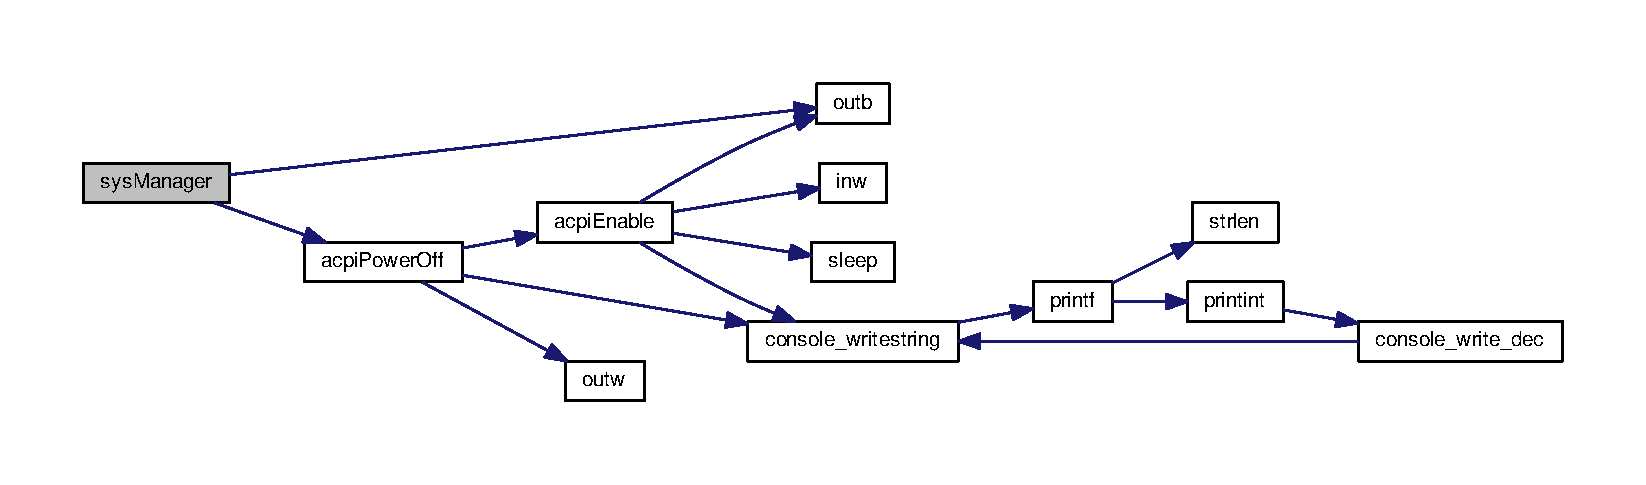
\includegraphics[width=350pt]{sys_8h_aabf1843b9c8b481005ecaa2db28447c1_cgraph}
\end{center}
\end{figure}



\hypertarget{cdefs_8h}{}\section{Experimental Edition/\+Library/sys/cdefs.h File Reference}
\label{cdefs_8h}\index{Experimental Edition/\+Library/sys/cdefs.\+h@{Experimental Edition/\+Library/sys/cdefs.\+h}}
This graph shows which files directly or indirectly include this file\+:
\nopagebreak
\begin{figure}[H]
\begin{center}
\leavevmode
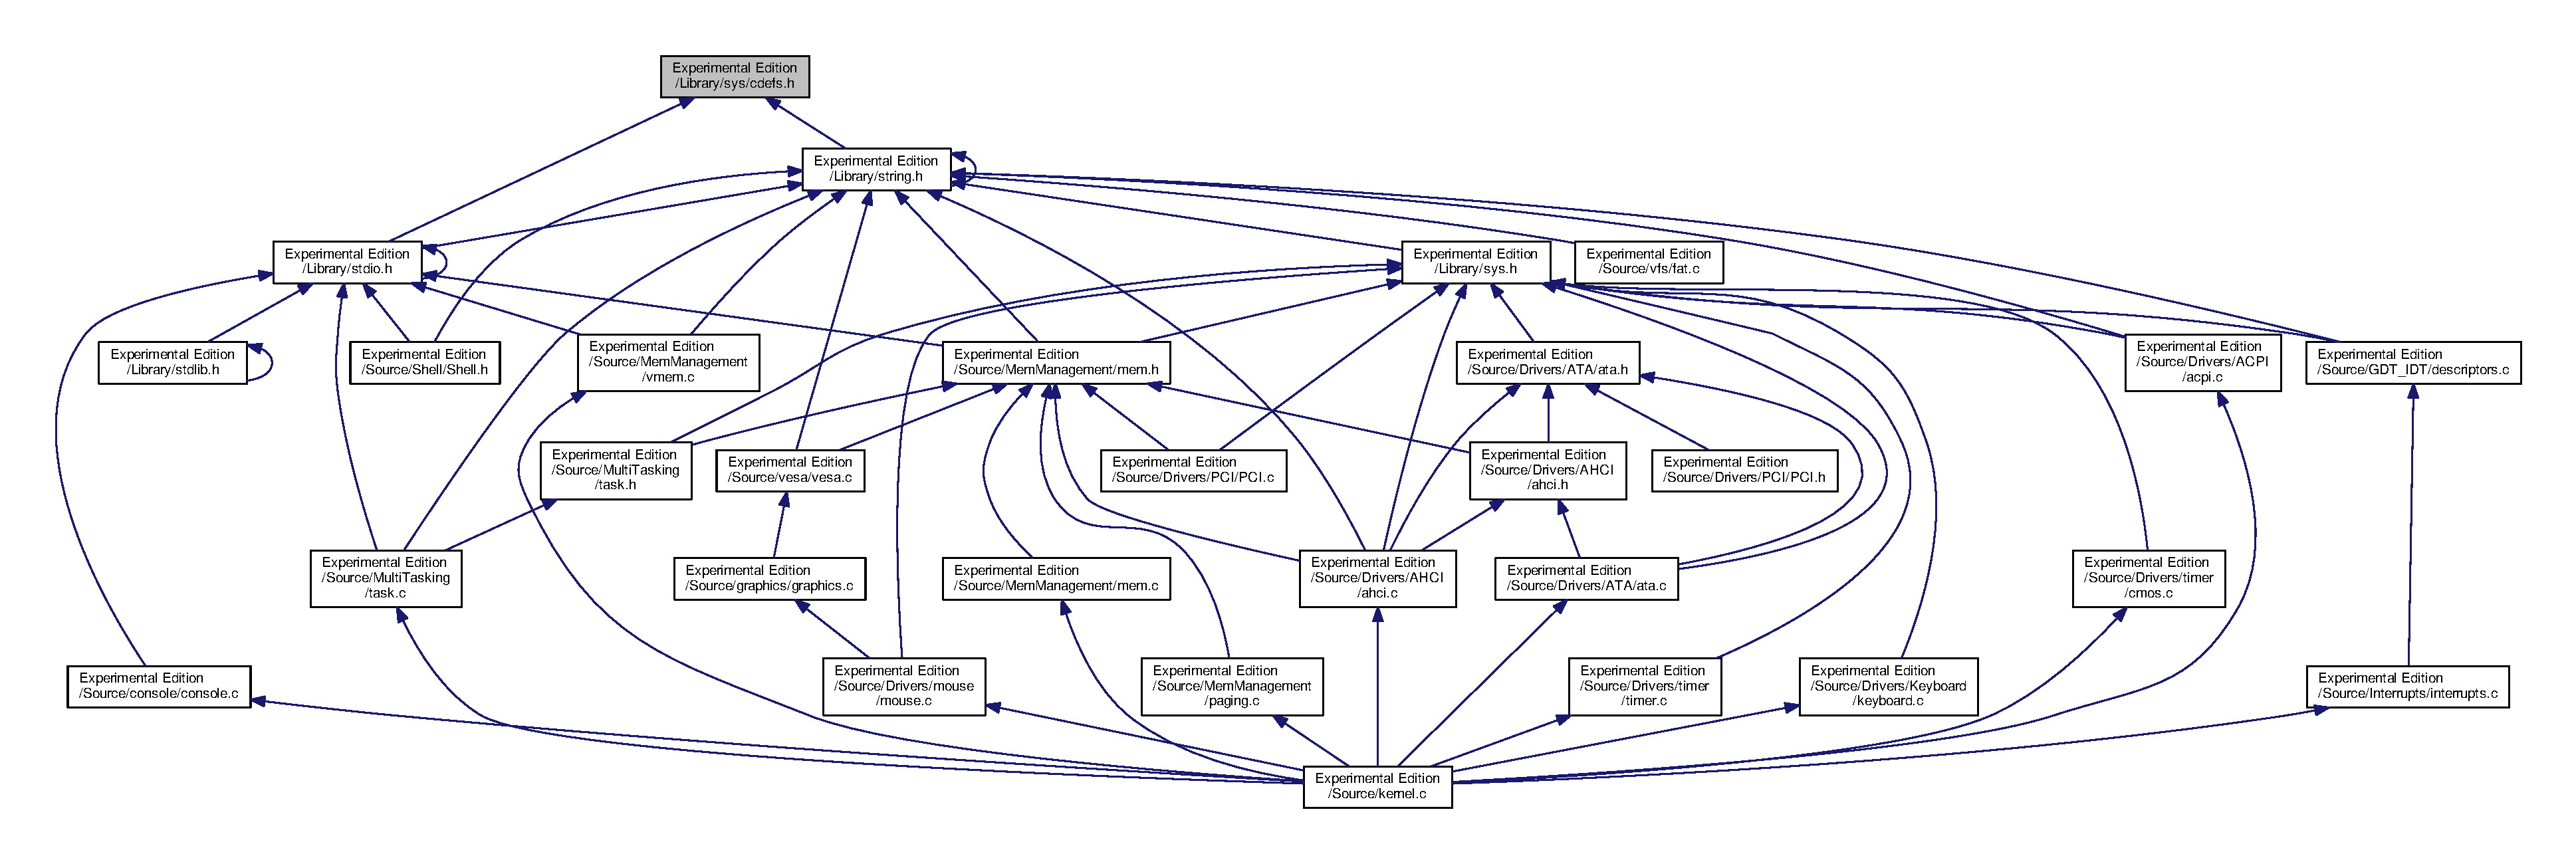
\includegraphics[width=350pt]{cdefs_8h__dep__incl}
\end{center}
\end{figure}
\subsection*{Macros}
\begin{DoxyCompactItemize}
\item 
\#define \hyperlink{cdefs_8h_a2116d823cc570512a208931843f054ac}{\+\_\+\+\_\+myos\+\_\+libc}~1
\end{DoxyCompactItemize}


\subsection{Macro Definition Documentation}
\index{cdefs.\+h@{cdefs.\+h}!\+\_\+\+\_\+myos\+\_\+libc@{\+\_\+\+\_\+myos\+\_\+libc}}
\index{\+\_\+\+\_\+myos\+\_\+libc@{\+\_\+\+\_\+myos\+\_\+libc}!cdefs.\+h@{cdefs.\+h}}
\subsubsection[{\texorpdfstring{\+\_\+\+\_\+myos\+\_\+libc}{__myos_libc}}]{\setlength{\rightskip}{0pt plus 5cm}\#define \+\_\+\+\_\+myos\+\_\+libc~1}\hypertarget{cdefs_8h_a2116d823cc570512a208931843f054ac}{}\label{cdefs_8h_a2116d823cc570512a208931843f054ac}


Definition at line 4 of file cdefs.\+h.


\hypertarget{system_8h}{}\section{Experimental Edition/\+Library/system.h File Reference}
\label{system_8h}\index{Experimental Edition/\+Library/system.\+h@{Experimental Edition/\+Library/system.\+h}}
This graph shows which files directly or indirectly include this file\+:
\nopagebreak
\begin{figure}[H]
\begin{center}
\leavevmode
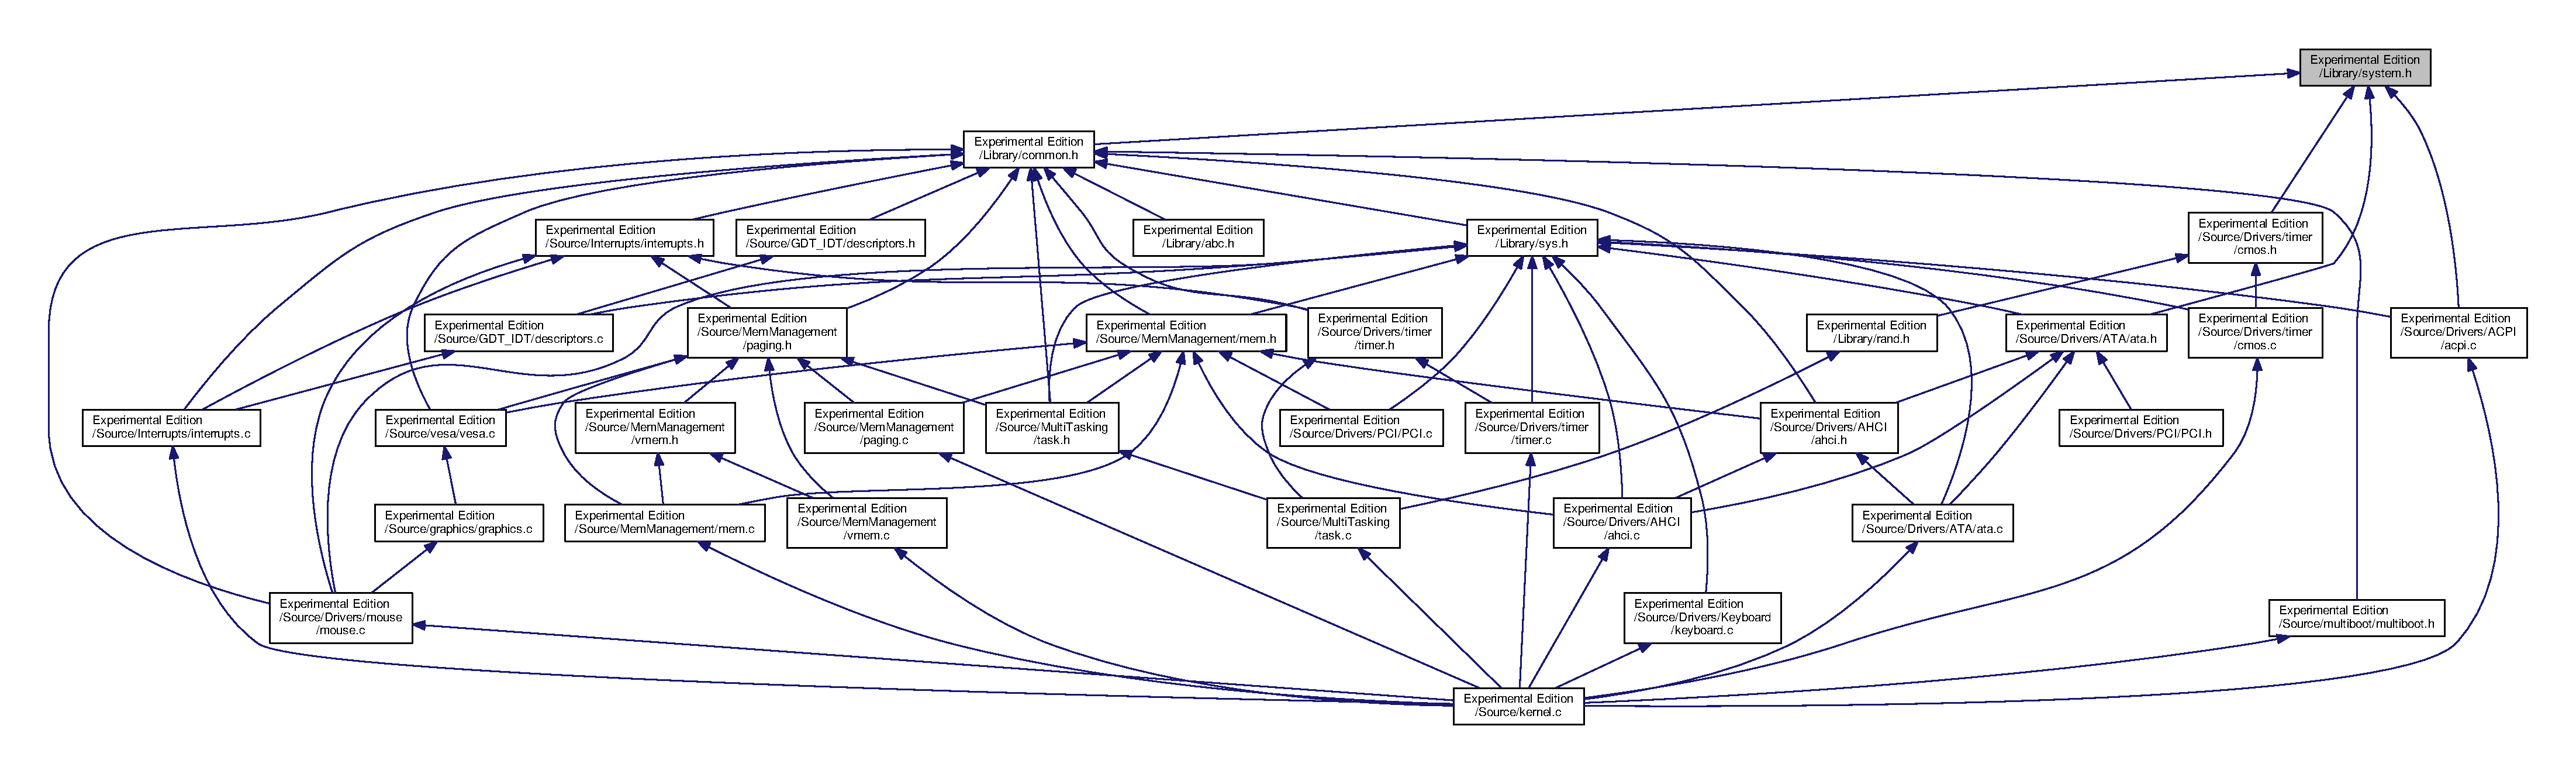
\includegraphics[width=350pt]{system_8h__dep__incl}
\end{center}
\end{figure}
\subsection*{Data Structures}
\begin{DoxyCompactItemize}
\item 
struct \hyperlink{structregs}{regs}
\end{DoxyCompactItemize}
\subsection*{Macros}
\begin{DoxyCompactItemize}
\item 
\#define \hyperlink{system_8h_a8885a13da4dafeb2cb209ce1b7ec3107}{I\+R\+Q0}~32
\item 
\#define \hyperlink{system_8h_a37360776bcc1dd3b5da93b025177551f}{I\+R\+Q1}~33
\item 
\#define \hyperlink{system_8h_a5388784cb69a0b869c4e5f60c839ca24}{I\+R\+Q2}~34
\item 
\#define \hyperlink{system_8h_a81b769ff26428bc3b6f20cb46096f4a2}{I\+R\+Q3}~35
\item 
\#define \hyperlink{system_8h_a3e56e05fa9adf8ddaaf6f44d999017db}{I\+R\+Q4}~36
\item 
\#define \hyperlink{system_8h_af1bd5ba58767b60d0639bd1a096dfdd6}{I\+R\+Q5}~37
\item 
\#define \hyperlink{system_8h_a1282e4c3484ca4c0689e180c5a42a7a9}{I\+R\+Q6}~38
\item 
\#define \hyperlink{system_8h_ac56b9fd6a60941e7594f299521575ca2}{I\+R\+Q7}~39
\item 
\#define \hyperlink{system_8h_ad299f4a78ead6e9f10cfa55376be25ac}{I\+R\+Q8}~40
\item 
\#define \hyperlink{system_8h_af59ffb9e0de6a5a1f9078a110460a2f4}{I\+R\+Q9}~41
\item 
\#define \hyperlink{system_8h_a4937470287000533f2dc2d0c29b88245}{I\+R\+Q10}~42
\item 
\#define \hyperlink{system_8h_afb33d89dcebc322429644b7ce8d3d629}{I\+R\+Q11}~43
\item 
\#define \hyperlink{system_8h_a57276d1481230d81d2bba849f935ce5a}{I\+R\+Q12}~44
\item 
\#define \hyperlink{system_8h_a13f5cba42d2e033d546107a80aa341ea}{I\+R\+Q13}~45
\item 
\#define \hyperlink{system_8h_a9577b9424e1d50ffb437da2a7052f391}{I\+R\+Q14}~46
\item 
\#define \hyperlink{system_8h_a587f058bf281246693f934ab414f7d52}{I\+R\+Q15}~47
\item 
\#define \hyperlink{system_8h_a186cc29999aa7cb635b5a54210f278df}{I\+N\+T\+E\+L\+S\+Y\+N\+T\+AX}~( asm ( \char`\"{}.intel\+\_\+syntax noprefix\char`\"{} ) )
\item 
\#define \hyperlink{system_8h_a0fdcfa3188ba6bf54a3814be27ea74bb}{A\+T\+T\+S\+Y\+N\+T\+AX}~( asm ( \char`\"{}.att\+\_\+syntax\char`\"{} ) )
\item 
\#define \hyperlink{system_8h_a070d2ce7b6bb7e5c05602aa8c308d0c4}{N\+U\+LL}~((void$\ast$)0)
\end{DoxyCompactItemize}
\subsection*{Typedefs}
\begin{DoxyCompactItemize}
\item 
typedef struct \hyperlink{structregs}{regs} $\ast$ \hyperlink{system_8h_ab0560cb0d0815e398c7d2aed26e54dc4}{M\+O\+U\+S\+E\+\_\+\+H\+A\+N\+D\+LE}
\item 
typedef unsigned int \hyperlink{system_8h_a12a1e9b3ce141648783a82445d02b58d}{uint\+\_\+t}
\end{DoxyCompactItemize}
\subsection*{Functions}
\begin{DoxyCompactItemize}
\item 
unsigned int \hyperlink{system_8h_a7fdcf079cdcd4af620e015f8226aca45}{read\+\_\+cr0} ()
\item 
void \hyperlink{system_8h_aac4f58f65812cf2b1d7deedd27ca02bb}{write\+\_\+cr0} (unsigned int cr0)
\end{DoxyCompactItemize}


\subsection{Macro Definition Documentation}
\index{system.\+h@{system.\+h}!A\+T\+T\+S\+Y\+N\+T\+AX@{A\+T\+T\+S\+Y\+N\+T\+AX}}
\index{A\+T\+T\+S\+Y\+N\+T\+AX@{A\+T\+T\+S\+Y\+N\+T\+AX}!system.\+h@{system.\+h}}
\subsubsection[{\texorpdfstring{A\+T\+T\+S\+Y\+N\+T\+AX}{ATTSYNTAX}}]{\setlength{\rightskip}{0pt plus 5cm}\#define A\+T\+T\+S\+Y\+N\+T\+AX~( asm ( \char`\"{}.att\+\_\+syntax\char`\"{} ) )}\hypertarget{system_8h_a0fdcfa3188ba6bf54a3814be27ea74bb}{}\label{system_8h_a0fdcfa3188ba6bf54a3814be27ea74bb}


Definition at line 32 of file system.\+h.

\index{system.\+h@{system.\+h}!I\+N\+T\+E\+L\+S\+Y\+N\+T\+AX@{I\+N\+T\+E\+L\+S\+Y\+N\+T\+AX}}
\index{I\+N\+T\+E\+L\+S\+Y\+N\+T\+AX@{I\+N\+T\+E\+L\+S\+Y\+N\+T\+AX}!system.\+h@{system.\+h}}
\subsubsection[{\texorpdfstring{I\+N\+T\+E\+L\+S\+Y\+N\+T\+AX}{INTELSYNTAX}}]{\setlength{\rightskip}{0pt plus 5cm}\#define I\+N\+T\+E\+L\+S\+Y\+N\+T\+AX~( asm ( \char`\"{}.intel\+\_\+syntax noprefix\char`\"{} ) )}\hypertarget{system_8h_a186cc29999aa7cb635b5a54210f278df}{}\label{system_8h_a186cc29999aa7cb635b5a54210f278df}


Definition at line 31 of file system.\+h.

\index{system.\+h@{system.\+h}!I\+R\+Q0@{I\+R\+Q0}}
\index{I\+R\+Q0@{I\+R\+Q0}!system.\+h@{system.\+h}}
\subsubsection[{\texorpdfstring{I\+R\+Q0}{IRQ0}}]{\setlength{\rightskip}{0pt plus 5cm}\#define I\+R\+Q0~32}\hypertarget{system_8h_a8885a13da4dafeb2cb209ce1b7ec3107}{}\label{system_8h_a8885a13da4dafeb2cb209ce1b7ec3107}


Definition at line 1 of file system.\+h.

\index{system.\+h@{system.\+h}!I\+R\+Q1@{I\+R\+Q1}}
\index{I\+R\+Q1@{I\+R\+Q1}!system.\+h@{system.\+h}}
\subsubsection[{\texorpdfstring{I\+R\+Q1}{IRQ1}}]{\setlength{\rightskip}{0pt plus 5cm}\#define I\+R\+Q1~33}\hypertarget{system_8h_a37360776bcc1dd3b5da93b025177551f}{}\label{system_8h_a37360776bcc1dd3b5da93b025177551f}


Definition at line 2 of file system.\+h.

\index{system.\+h@{system.\+h}!I\+R\+Q10@{I\+R\+Q10}}
\index{I\+R\+Q10@{I\+R\+Q10}!system.\+h@{system.\+h}}
\subsubsection[{\texorpdfstring{I\+R\+Q10}{IRQ10}}]{\setlength{\rightskip}{0pt plus 5cm}\#define I\+R\+Q10~42}\hypertarget{system_8h_a4937470287000533f2dc2d0c29b88245}{}\label{system_8h_a4937470287000533f2dc2d0c29b88245}


Definition at line 11 of file system.\+h.

\index{system.\+h@{system.\+h}!I\+R\+Q11@{I\+R\+Q11}}
\index{I\+R\+Q11@{I\+R\+Q11}!system.\+h@{system.\+h}}
\subsubsection[{\texorpdfstring{I\+R\+Q11}{IRQ11}}]{\setlength{\rightskip}{0pt plus 5cm}\#define I\+R\+Q11~43}\hypertarget{system_8h_afb33d89dcebc322429644b7ce8d3d629}{}\label{system_8h_afb33d89dcebc322429644b7ce8d3d629}


Definition at line 12 of file system.\+h.

\index{system.\+h@{system.\+h}!I\+R\+Q12@{I\+R\+Q12}}
\index{I\+R\+Q12@{I\+R\+Q12}!system.\+h@{system.\+h}}
\subsubsection[{\texorpdfstring{I\+R\+Q12}{IRQ12}}]{\setlength{\rightskip}{0pt plus 5cm}\#define I\+R\+Q12~44}\hypertarget{system_8h_a57276d1481230d81d2bba849f935ce5a}{}\label{system_8h_a57276d1481230d81d2bba849f935ce5a}


Definition at line 13 of file system.\+h.

\index{system.\+h@{system.\+h}!I\+R\+Q13@{I\+R\+Q13}}
\index{I\+R\+Q13@{I\+R\+Q13}!system.\+h@{system.\+h}}
\subsubsection[{\texorpdfstring{I\+R\+Q13}{IRQ13}}]{\setlength{\rightskip}{0pt plus 5cm}\#define I\+R\+Q13~45}\hypertarget{system_8h_a13f5cba42d2e033d546107a80aa341ea}{}\label{system_8h_a13f5cba42d2e033d546107a80aa341ea}


Definition at line 14 of file system.\+h.

\index{system.\+h@{system.\+h}!I\+R\+Q14@{I\+R\+Q14}}
\index{I\+R\+Q14@{I\+R\+Q14}!system.\+h@{system.\+h}}
\subsubsection[{\texorpdfstring{I\+R\+Q14}{IRQ14}}]{\setlength{\rightskip}{0pt plus 5cm}\#define I\+R\+Q14~46}\hypertarget{system_8h_a9577b9424e1d50ffb437da2a7052f391}{}\label{system_8h_a9577b9424e1d50ffb437da2a7052f391}


Definition at line 15 of file system.\+h.

\index{system.\+h@{system.\+h}!I\+R\+Q15@{I\+R\+Q15}}
\index{I\+R\+Q15@{I\+R\+Q15}!system.\+h@{system.\+h}}
\subsubsection[{\texorpdfstring{I\+R\+Q15}{IRQ15}}]{\setlength{\rightskip}{0pt plus 5cm}\#define I\+R\+Q15~47}\hypertarget{system_8h_a587f058bf281246693f934ab414f7d52}{}\label{system_8h_a587f058bf281246693f934ab414f7d52}


Definition at line 16 of file system.\+h.

\index{system.\+h@{system.\+h}!I\+R\+Q2@{I\+R\+Q2}}
\index{I\+R\+Q2@{I\+R\+Q2}!system.\+h@{system.\+h}}
\subsubsection[{\texorpdfstring{I\+R\+Q2}{IRQ2}}]{\setlength{\rightskip}{0pt plus 5cm}\#define I\+R\+Q2~34}\hypertarget{system_8h_a5388784cb69a0b869c4e5f60c839ca24}{}\label{system_8h_a5388784cb69a0b869c4e5f60c839ca24}


Definition at line 3 of file system.\+h.

\index{system.\+h@{system.\+h}!I\+R\+Q3@{I\+R\+Q3}}
\index{I\+R\+Q3@{I\+R\+Q3}!system.\+h@{system.\+h}}
\subsubsection[{\texorpdfstring{I\+R\+Q3}{IRQ3}}]{\setlength{\rightskip}{0pt plus 5cm}\#define I\+R\+Q3~35}\hypertarget{system_8h_a81b769ff26428bc3b6f20cb46096f4a2}{}\label{system_8h_a81b769ff26428bc3b6f20cb46096f4a2}


Definition at line 4 of file system.\+h.

\index{system.\+h@{system.\+h}!I\+R\+Q4@{I\+R\+Q4}}
\index{I\+R\+Q4@{I\+R\+Q4}!system.\+h@{system.\+h}}
\subsubsection[{\texorpdfstring{I\+R\+Q4}{IRQ4}}]{\setlength{\rightskip}{0pt plus 5cm}\#define I\+R\+Q4~36}\hypertarget{system_8h_a3e56e05fa9adf8ddaaf6f44d999017db}{}\label{system_8h_a3e56e05fa9adf8ddaaf6f44d999017db}


Definition at line 5 of file system.\+h.

\index{system.\+h@{system.\+h}!I\+R\+Q5@{I\+R\+Q5}}
\index{I\+R\+Q5@{I\+R\+Q5}!system.\+h@{system.\+h}}
\subsubsection[{\texorpdfstring{I\+R\+Q5}{IRQ5}}]{\setlength{\rightskip}{0pt plus 5cm}\#define I\+R\+Q5~37}\hypertarget{system_8h_af1bd5ba58767b60d0639bd1a096dfdd6}{}\label{system_8h_af1bd5ba58767b60d0639bd1a096dfdd6}


Definition at line 6 of file system.\+h.

\index{system.\+h@{system.\+h}!I\+R\+Q6@{I\+R\+Q6}}
\index{I\+R\+Q6@{I\+R\+Q6}!system.\+h@{system.\+h}}
\subsubsection[{\texorpdfstring{I\+R\+Q6}{IRQ6}}]{\setlength{\rightskip}{0pt plus 5cm}\#define I\+R\+Q6~38}\hypertarget{system_8h_a1282e4c3484ca4c0689e180c5a42a7a9}{}\label{system_8h_a1282e4c3484ca4c0689e180c5a42a7a9}


Definition at line 7 of file system.\+h.

\index{system.\+h@{system.\+h}!I\+R\+Q7@{I\+R\+Q7}}
\index{I\+R\+Q7@{I\+R\+Q7}!system.\+h@{system.\+h}}
\subsubsection[{\texorpdfstring{I\+R\+Q7}{IRQ7}}]{\setlength{\rightskip}{0pt plus 5cm}\#define I\+R\+Q7~39}\hypertarget{system_8h_ac56b9fd6a60941e7594f299521575ca2}{}\label{system_8h_ac56b9fd6a60941e7594f299521575ca2}


Definition at line 8 of file system.\+h.

\index{system.\+h@{system.\+h}!I\+R\+Q8@{I\+R\+Q8}}
\index{I\+R\+Q8@{I\+R\+Q8}!system.\+h@{system.\+h}}
\subsubsection[{\texorpdfstring{I\+R\+Q8}{IRQ8}}]{\setlength{\rightskip}{0pt plus 5cm}\#define I\+R\+Q8~40}\hypertarget{system_8h_ad299f4a78ead6e9f10cfa55376be25ac}{}\label{system_8h_ad299f4a78ead6e9f10cfa55376be25ac}


Definition at line 9 of file system.\+h.

\index{system.\+h@{system.\+h}!I\+R\+Q9@{I\+R\+Q9}}
\index{I\+R\+Q9@{I\+R\+Q9}!system.\+h@{system.\+h}}
\subsubsection[{\texorpdfstring{I\+R\+Q9}{IRQ9}}]{\setlength{\rightskip}{0pt plus 5cm}\#define I\+R\+Q9~41}\hypertarget{system_8h_af59ffb9e0de6a5a1f9078a110460a2f4}{}\label{system_8h_af59ffb9e0de6a5a1f9078a110460a2f4}


Definition at line 10 of file system.\+h.

\index{system.\+h@{system.\+h}!N\+U\+LL@{N\+U\+LL}}
\index{N\+U\+LL@{N\+U\+LL}!system.\+h@{system.\+h}}
\subsubsection[{\texorpdfstring{N\+U\+LL}{NULL}}]{\setlength{\rightskip}{0pt plus 5cm}\#define N\+U\+LL~((void$\ast$)0)}\hypertarget{system_8h_a070d2ce7b6bb7e5c05602aa8c308d0c4}{}\label{system_8h_a070d2ce7b6bb7e5c05602aa8c308d0c4}


Definition at line 43 of file system.\+h.



\subsection{Typedef Documentation}
\index{system.\+h@{system.\+h}!M\+O\+U\+S\+E\+\_\+\+H\+A\+N\+D\+LE@{M\+O\+U\+S\+E\+\_\+\+H\+A\+N\+D\+LE}}
\index{M\+O\+U\+S\+E\+\_\+\+H\+A\+N\+D\+LE@{M\+O\+U\+S\+E\+\_\+\+H\+A\+N\+D\+LE}!system.\+h@{system.\+h}}
\subsubsection[{\texorpdfstring{M\+O\+U\+S\+E\+\_\+\+H\+A\+N\+D\+LE}{MOUSE_HANDLE}}]{\setlength{\rightskip}{0pt plus 5cm}typedef struct {\bf regs}$\ast$ {\bf M\+O\+U\+S\+E\+\_\+\+H\+A\+N\+D\+LE}}\hypertarget{system_8h_ab0560cb0d0815e398c7d2aed26e54dc4}{}\label{system_8h_ab0560cb0d0815e398c7d2aed26e54dc4}
\index{system.\+h@{system.\+h}!uint\+\_\+t@{uint\+\_\+t}}
\index{uint\+\_\+t@{uint\+\_\+t}!system.\+h@{system.\+h}}
\subsubsection[{\texorpdfstring{uint\+\_\+t}{uint_t}}]{\setlength{\rightskip}{0pt plus 5cm}typedef unsigned int {\bf uint\+\_\+t}}\hypertarget{system_8h_a12a1e9b3ce141648783a82445d02b58d}{}\label{system_8h_a12a1e9b3ce141648783a82445d02b58d}


Definition at line 39 of file system.\+h.



\subsection{Function Documentation}
\index{system.\+h@{system.\+h}!read\+\_\+cr0@{read\+\_\+cr0}}
\index{read\+\_\+cr0@{read\+\_\+cr0}!system.\+h@{system.\+h}}
\subsubsection[{\texorpdfstring{read\+\_\+cr0()}{read_cr0()}}]{\setlength{\rightskip}{0pt plus 5cm}unsigned int read\+\_\+cr0 (
\begin{DoxyParamCaption}
{}
\end{DoxyParamCaption}
)}\hypertarget{system_8h_a7fdcf079cdcd4af620e015f8226aca45}{}\label{system_8h_a7fdcf079cdcd4af620e015f8226aca45}
\index{system.\+h@{system.\+h}!write\+\_\+cr0@{write\+\_\+cr0}}
\index{write\+\_\+cr0@{write\+\_\+cr0}!system.\+h@{system.\+h}}
\subsubsection[{\texorpdfstring{write\+\_\+cr0(unsigned int cr0)}{write_cr0(unsigned int cr0)}}]{\setlength{\rightskip}{0pt plus 5cm}void write\+\_\+cr0 (
\begin{DoxyParamCaption}
\item[{unsigned int}]{cr0}
\end{DoxyParamCaption}
)}\hypertarget{system_8h_aac4f58f65812cf2b1d7deedd27ca02bb}{}\label{system_8h_aac4f58f65812cf2b1d7deedd27ca02bb}

\hypertarget{switch_8asm}{}\section{Experimental Edition/nasm/arch/x86/switch.asm File Reference}
\label{switch_8asm}\index{Experimental Edition/nasm/arch/x86/switch.\+asm@{Experimental Edition/nasm/arch/x86/switch.\+asm}}

\hypertarget{v86_8asm}{}\section{Experimental Edition/nasm/arch/x86/v86.asm File Reference}
\label{v86_8asm}\index{Experimental Edition/nasm/arch/x86/v86.\+asm@{Experimental Edition/nasm/arch/x86/v86.\+asm}}

\hypertarget{boot_8S}{}\section{Experimental Edition/\+Source/arch/x86/boot.S File Reference}
\label{boot_8S}\index{Experimental Edition/\+Source/arch/x86/boot.\+S@{Experimental Edition/\+Source/arch/x86/boot.\+S}}

\hypertarget{descriptors_8asm}{}\section{Experimental Edition/\+Source/arch/x86/descriptors.asm File Reference}
\label{descriptors_8asm}\index{Experimental Edition/\+Source/arch/x86/descriptors.\+asm@{Experimental Edition/\+Source/arch/x86/descriptors.\+asm}}

\hypertarget{interrupts_8s}{}\section{Experimental Edition/\+Source/arch/x86/interrupts.s File Reference}
\label{interrupts_8s}\index{Experimental Edition/\+Source/arch/x86/interrupts.\+s@{Experimental Edition/\+Source/arch/x86/interrupts.\+s}}

\hypertarget{multiboot_8s}{}\section{Experimental Edition/\+Source/arch/x86/multiboot.s File Reference}
\label{multiboot_8s}\index{Experimental Edition/\+Source/arch/x86/multiboot.\+s@{Experimental Edition/\+Source/arch/x86/multiboot.\+s}}

\hypertarget{process_8s}{}\section{Experimental Edition/\+Source/arch/x86/process.s File Reference}
\label{process_8s}\index{Experimental Edition/\+Source/arch/x86/process.\+s@{Experimental Edition/\+Source/arch/x86/process.\+s}}

\hypertarget{switchTask_8s}{}\section{Experimental Edition/\+Source/arch/x86/switch\+Task.s File Reference}
\label{switchTask_8s}\index{Experimental Edition/\+Source/arch/x86/switch\+Task.\+s@{Experimental Edition/\+Source/arch/x86/switch\+Task.\+s}}

\hypertarget{vga_8h}{}\section{Experimental Edition/\+Source/console/arch/x86/vga.h File Reference}
\label{vga_8h}\index{Experimental Edition/\+Source/console/arch/x86/vga.\+h@{Experimental Edition/\+Source/console/arch/x86/vga.\+h}}
This graph shows which files directly or indirectly include this file\+:
\nopagebreak
\begin{figure}[H]
\begin{center}
\leavevmode
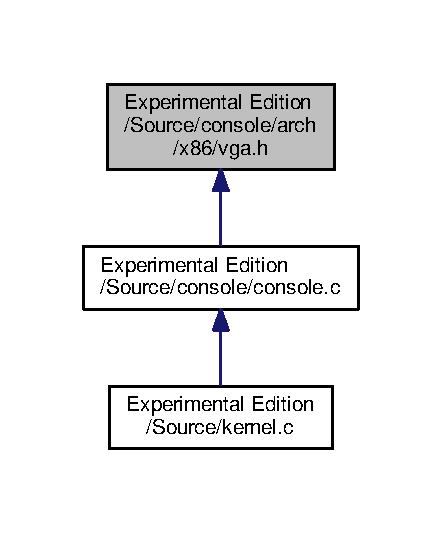
\includegraphics[width=212pt]{vga_8h__dep__incl}
\end{center}
\end{figure}
\subsection*{Enumerations}
\begin{DoxyCompactItemize}
\item 
enum \hyperlink{vga_8h_abaae057bae62d0c3e11501e3199cb60e}{vga\+\_\+color} \{ \\*
\hyperlink{vga_8h_abaae057bae62d0c3e11501e3199cb60ea2a9daf215a30f1c539ead18c66380fc1}{C\+O\+L\+O\+R\+\_\+\+B\+L\+A\+CK} = 0, 
\hyperlink{vga_8h_abaae057bae62d0c3e11501e3199cb60ea1340428efccb140dcbdb71aa6176f696}{C\+O\+L\+O\+R\+\_\+\+B\+L\+UE} = 1, 
\hyperlink{vga_8h_abaae057bae62d0c3e11501e3199cb60eacfa9d8bbffc418447ed826f286abca02}{C\+O\+L\+O\+R\+\_\+\+G\+R\+E\+EN} = 2, 
\hyperlink{vga_8h_abaae057bae62d0c3e11501e3199cb60ea7896ff2cc707b5873da0b97d38bf852e}{C\+O\+L\+O\+R\+\_\+\+C\+Y\+AN} = 3, 
\\*
\hyperlink{vga_8h_abaae057bae62d0c3e11501e3199cb60ea592503b9434c1e751a92f3fc536d7950}{C\+O\+L\+O\+R\+\_\+\+R\+ED} = 4, 
\hyperlink{vga_8h_abaae057bae62d0c3e11501e3199cb60ea543701a16830d494b0e460cccf0f9b37}{C\+O\+L\+O\+R\+\_\+\+M\+A\+G\+E\+N\+TA} = 5, 
\hyperlink{vga_8h_abaae057bae62d0c3e11501e3199cb60ea70b424bcf0a4a80c0a6f810d1cff20fe}{C\+O\+L\+O\+R\+\_\+\+B\+R\+O\+WN} = 6, 
\hyperlink{vga_8h_abaae057bae62d0c3e11501e3199cb60ea612e88bdf4015d1f208761d40c603a0e}{C\+O\+L\+O\+R\+\_\+\+L\+I\+G\+H\+T\+\_\+\+G\+R\+EY} = 7, 
\\*
\hyperlink{vga_8h_abaae057bae62d0c3e11501e3199cb60ea45d9d75a762b11d0a1f5b6f65bf59b48}{C\+O\+L\+O\+R\+\_\+\+D\+A\+R\+K\+\_\+\+G\+R\+EY} = 8, 
\hyperlink{vga_8h_abaae057bae62d0c3e11501e3199cb60ea97e4b144ec0f5f6a6d19eccd00a1cba8}{C\+O\+L\+O\+R\+\_\+\+L\+I\+G\+H\+T\+\_\+\+B\+L\+UE} = 9, 
\hyperlink{vga_8h_abaae057bae62d0c3e11501e3199cb60ea35ff3a3ccb655f1e72e7c0c74588e41b}{C\+O\+L\+O\+R\+\_\+\+L\+I\+G\+H\+T\+\_\+\+G\+R\+E\+EN} = 10, 
\hyperlink{vga_8h_abaae057bae62d0c3e11501e3199cb60eaceba56a8aca3ee9dfc0383c5a35cbabe}{C\+O\+L\+O\+R\+\_\+\+L\+I\+G\+H\+T\+\_\+\+C\+Y\+AN} = 11, 
\\*
\hyperlink{vga_8h_abaae057bae62d0c3e11501e3199cb60ea726df597a3d842789899ff84f7ff3721}{C\+O\+L\+O\+R\+\_\+\+L\+I\+G\+H\+T\+\_\+\+R\+ED} = 12, 
\hyperlink{vga_8h_abaae057bae62d0c3e11501e3199cb60ea03a14ea206d5ae22b371b4b707bb7909}{C\+O\+L\+O\+R\+\_\+\+L\+I\+G\+H\+T\+\_\+\+M\+A\+G\+E\+N\+TA} = 13, 
\hyperlink{vga_8h_abaae057bae62d0c3e11501e3199cb60ea191ffff15801f584eb332e08b1f3aba3}{C\+O\+L\+O\+R\+\_\+\+L\+I\+G\+H\+T\+\_\+\+B\+R\+O\+WN} = 14, 
\hyperlink{vga_8h_abaae057bae62d0c3e11501e3199cb60ead47b4c240a0109970bb2a7fe3a07d3ec}{C\+O\+L\+O\+R\+\_\+\+W\+H\+I\+TE} = 15
 \}
\end{DoxyCompactItemize}


\subsection{Enumeration Type Documentation}
\index{vga.\+h@{vga.\+h}!vga\+\_\+color@{vga\+\_\+color}}
\index{vga\+\_\+color@{vga\+\_\+color}!vga.\+h@{vga.\+h}}
\subsubsection[{\texorpdfstring{vga\+\_\+color}{vga_color}}]{\setlength{\rightskip}{0pt plus 5cm}enum {\bf vga\+\_\+color}}\hypertarget{vga_8h_abaae057bae62d0c3e11501e3199cb60e}{}\label{vga_8h_abaae057bae62d0c3e11501e3199cb60e}
\begin{Desc}
\item[Enumerator]\par
\begin{description}
\index{C\+O\+L\+O\+R\+\_\+\+B\+L\+A\+CK@{C\+O\+L\+O\+R\+\_\+\+B\+L\+A\+CK}!vga.\+h@{vga.\+h}}\index{vga.\+h@{vga.\+h}!C\+O\+L\+O\+R\+\_\+\+B\+L\+A\+CK@{C\+O\+L\+O\+R\+\_\+\+B\+L\+A\+CK}}\item[{\em 
C\+O\+L\+O\+R\+\_\+\+B\+L\+A\+CK\hypertarget{vga_8h_abaae057bae62d0c3e11501e3199cb60ea2a9daf215a30f1c539ead18c66380fc1}{}\label{vga_8h_abaae057bae62d0c3e11501e3199cb60ea2a9daf215a30f1c539ead18c66380fc1}
}]\index{C\+O\+L\+O\+R\+\_\+\+B\+L\+UE@{C\+O\+L\+O\+R\+\_\+\+B\+L\+UE}!vga.\+h@{vga.\+h}}\index{vga.\+h@{vga.\+h}!C\+O\+L\+O\+R\+\_\+\+B\+L\+UE@{C\+O\+L\+O\+R\+\_\+\+B\+L\+UE}}\item[{\em 
C\+O\+L\+O\+R\+\_\+\+B\+L\+UE\hypertarget{vga_8h_abaae057bae62d0c3e11501e3199cb60ea1340428efccb140dcbdb71aa6176f696}{}\label{vga_8h_abaae057bae62d0c3e11501e3199cb60ea1340428efccb140dcbdb71aa6176f696}
}]\index{C\+O\+L\+O\+R\+\_\+\+G\+R\+E\+EN@{C\+O\+L\+O\+R\+\_\+\+G\+R\+E\+EN}!vga.\+h@{vga.\+h}}\index{vga.\+h@{vga.\+h}!C\+O\+L\+O\+R\+\_\+\+G\+R\+E\+EN@{C\+O\+L\+O\+R\+\_\+\+G\+R\+E\+EN}}\item[{\em 
C\+O\+L\+O\+R\+\_\+\+G\+R\+E\+EN\hypertarget{vga_8h_abaae057bae62d0c3e11501e3199cb60eacfa9d8bbffc418447ed826f286abca02}{}\label{vga_8h_abaae057bae62d0c3e11501e3199cb60eacfa9d8bbffc418447ed826f286abca02}
}]\index{C\+O\+L\+O\+R\+\_\+\+C\+Y\+AN@{C\+O\+L\+O\+R\+\_\+\+C\+Y\+AN}!vga.\+h@{vga.\+h}}\index{vga.\+h@{vga.\+h}!C\+O\+L\+O\+R\+\_\+\+C\+Y\+AN@{C\+O\+L\+O\+R\+\_\+\+C\+Y\+AN}}\item[{\em 
C\+O\+L\+O\+R\+\_\+\+C\+Y\+AN\hypertarget{vga_8h_abaae057bae62d0c3e11501e3199cb60ea7896ff2cc707b5873da0b97d38bf852e}{}\label{vga_8h_abaae057bae62d0c3e11501e3199cb60ea7896ff2cc707b5873da0b97d38bf852e}
}]\index{C\+O\+L\+O\+R\+\_\+\+R\+ED@{C\+O\+L\+O\+R\+\_\+\+R\+ED}!vga.\+h@{vga.\+h}}\index{vga.\+h@{vga.\+h}!C\+O\+L\+O\+R\+\_\+\+R\+ED@{C\+O\+L\+O\+R\+\_\+\+R\+ED}}\item[{\em 
C\+O\+L\+O\+R\+\_\+\+R\+ED\hypertarget{vga_8h_abaae057bae62d0c3e11501e3199cb60ea592503b9434c1e751a92f3fc536d7950}{}\label{vga_8h_abaae057bae62d0c3e11501e3199cb60ea592503b9434c1e751a92f3fc536d7950}
}]\index{C\+O\+L\+O\+R\+\_\+\+M\+A\+G\+E\+N\+TA@{C\+O\+L\+O\+R\+\_\+\+M\+A\+G\+E\+N\+TA}!vga.\+h@{vga.\+h}}\index{vga.\+h@{vga.\+h}!C\+O\+L\+O\+R\+\_\+\+M\+A\+G\+E\+N\+TA@{C\+O\+L\+O\+R\+\_\+\+M\+A\+G\+E\+N\+TA}}\item[{\em 
C\+O\+L\+O\+R\+\_\+\+M\+A\+G\+E\+N\+TA\hypertarget{vga_8h_abaae057bae62d0c3e11501e3199cb60ea543701a16830d494b0e460cccf0f9b37}{}\label{vga_8h_abaae057bae62d0c3e11501e3199cb60ea543701a16830d494b0e460cccf0f9b37}
}]\index{C\+O\+L\+O\+R\+\_\+\+B\+R\+O\+WN@{C\+O\+L\+O\+R\+\_\+\+B\+R\+O\+WN}!vga.\+h@{vga.\+h}}\index{vga.\+h@{vga.\+h}!C\+O\+L\+O\+R\+\_\+\+B\+R\+O\+WN@{C\+O\+L\+O\+R\+\_\+\+B\+R\+O\+WN}}\item[{\em 
C\+O\+L\+O\+R\+\_\+\+B\+R\+O\+WN\hypertarget{vga_8h_abaae057bae62d0c3e11501e3199cb60ea70b424bcf0a4a80c0a6f810d1cff20fe}{}\label{vga_8h_abaae057bae62d0c3e11501e3199cb60ea70b424bcf0a4a80c0a6f810d1cff20fe}
}]\index{C\+O\+L\+O\+R\+\_\+\+L\+I\+G\+H\+T\+\_\+\+G\+R\+EY@{C\+O\+L\+O\+R\+\_\+\+L\+I\+G\+H\+T\+\_\+\+G\+R\+EY}!vga.\+h@{vga.\+h}}\index{vga.\+h@{vga.\+h}!C\+O\+L\+O\+R\+\_\+\+L\+I\+G\+H\+T\+\_\+\+G\+R\+EY@{C\+O\+L\+O\+R\+\_\+\+L\+I\+G\+H\+T\+\_\+\+G\+R\+EY}}\item[{\em 
C\+O\+L\+O\+R\+\_\+\+L\+I\+G\+H\+T\+\_\+\+G\+R\+EY\hypertarget{vga_8h_abaae057bae62d0c3e11501e3199cb60ea612e88bdf4015d1f208761d40c603a0e}{}\label{vga_8h_abaae057bae62d0c3e11501e3199cb60ea612e88bdf4015d1f208761d40c603a0e}
}]\index{C\+O\+L\+O\+R\+\_\+\+D\+A\+R\+K\+\_\+\+G\+R\+EY@{C\+O\+L\+O\+R\+\_\+\+D\+A\+R\+K\+\_\+\+G\+R\+EY}!vga.\+h@{vga.\+h}}\index{vga.\+h@{vga.\+h}!C\+O\+L\+O\+R\+\_\+\+D\+A\+R\+K\+\_\+\+G\+R\+EY@{C\+O\+L\+O\+R\+\_\+\+D\+A\+R\+K\+\_\+\+G\+R\+EY}}\item[{\em 
C\+O\+L\+O\+R\+\_\+\+D\+A\+R\+K\+\_\+\+G\+R\+EY\hypertarget{vga_8h_abaae057bae62d0c3e11501e3199cb60ea45d9d75a762b11d0a1f5b6f65bf59b48}{}\label{vga_8h_abaae057bae62d0c3e11501e3199cb60ea45d9d75a762b11d0a1f5b6f65bf59b48}
}]\index{C\+O\+L\+O\+R\+\_\+\+L\+I\+G\+H\+T\+\_\+\+B\+L\+UE@{C\+O\+L\+O\+R\+\_\+\+L\+I\+G\+H\+T\+\_\+\+B\+L\+UE}!vga.\+h@{vga.\+h}}\index{vga.\+h@{vga.\+h}!C\+O\+L\+O\+R\+\_\+\+L\+I\+G\+H\+T\+\_\+\+B\+L\+UE@{C\+O\+L\+O\+R\+\_\+\+L\+I\+G\+H\+T\+\_\+\+B\+L\+UE}}\item[{\em 
C\+O\+L\+O\+R\+\_\+\+L\+I\+G\+H\+T\+\_\+\+B\+L\+UE\hypertarget{vga_8h_abaae057bae62d0c3e11501e3199cb60ea97e4b144ec0f5f6a6d19eccd00a1cba8}{}\label{vga_8h_abaae057bae62d0c3e11501e3199cb60ea97e4b144ec0f5f6a6d19eccd00a1cba8}
}]\index{C\+O\+L\+O\+R\+\_\+\+L\+I\+G\+H\+T\+\_\+\+G\+R\+E\+EN@{C\+O\+L\+O\+R\+\_\+\+L\+I\+G\+H\+T\+\_\+\+G\+R\+E\+EN}!vga.\+h@{vga.\+h}}\index{vga.\+h@{vga.\+h}!C\+O\+L\+O\+R\+\_\+\+L\+I\+G\+H\+T\+\_\+\+G\+R\+E\+EN@{C\+O\+L\+O\+R\+\_\+\+L\+I\+G\+H\+T\+\_\+\+G\+R\+E\+EN}}\item[{\em 
C\+O\+L\+O\+R\+\_\+\+L\+I\+G\+H\+T\+\_\+\+G\+R\+E\+EN\hypertarget{vga_8h_abaae057bae62d0c3e11501e3199cb60ea35ff3a3ccb655f1e72e7c0c74588e41b}{}\label{vga_8h_abaae057bae62d0c3e11501e3199cb60ea35ff3a3ccb655f1e72e7c0c74588e41b}
}]\index{C\+O\+L\+O\+R\+\_\+\+L\+I\+G\+H\+T\+\_\+\+C\+Y\+AN@{C\+O\+L\+O\+R\+\_\+\+L\+I\+G\+H\+T\+\_\+\+C\+Y\+AN}!vga.\+h@{vga.\+h}}\index{vga.\+h@{vga.\+h}!C\+O\+L\+O\+R\+\_\+\+L\+I\+G\+H\+T\+\_\+\+C\+Y\+AN@{C\+O\+L\+O\+R\+\_\+\+L\+I\+G\+H\+T\+\_\+\+C\+Y\+AN}}\item[{\em 
C\+O\+L\+O\+R\+\_\+\+L\+I\+G\+H\+T\+\_\+\+C\+Y\+AN\hypertarget{vga_8h_abaae057bae62d0c3e11501e3199cb60eaceba56a8aca3ee9dfc0383c5a35cbabe}{}\label{vga_8h_abaae057bae62d0c3e11501e3199cb60eaceba56a8aca3ee9dfc0383c5a35cbabe}
}]\index{C\+O\+L\+O\+R\+\_\+\+L\+I\+G\+H\+T\+\_\+\+R\+ED@{C\+O\+L\+O\+R\+\_\+\+L\+I\+G\+H\+T\+\_\+\+R\+ED}!vga.\+h@{vga.\+h}}\index{vga.\+h@{vga.\+h}!C\+O\+L\+O\+R\+\_\+\+L\+I\+G\+H\+T\+\_\+\+R\+ED@{C\+O\+L\+O\+R\+\_\+\+L\+I\+G\+H\+T\+\_\+\+R\+ED}}\item[{\em 
C\+O\+L\+O\+R\+\_\+\+L\+I\+G\+H\+T\+\_\+\+R\+ED\hypertarget{vga_8h_abaae057bae62d0c3e11501e3199cb60ea726df597a3d842789899ff84f7ff3721}{}\label{vga_8h_abaae057bae62d0c3e11501e3199cb60ea726df597a3d842789899ff84f7ff3721}
}]\index{C\+O\+L\+O\+R\+\_\+\+L\+I\+G\+H\+T\+\_\+\+M\+A\+G\+E\+N\+TA@{C\+O\+L\+O\+R\+\_\+\+L\+I\+G\+H\+T\+\_\+\+M\+A\+G\+E\+N\+TA}!vga.\+h@{vga.\+h}}\index{vga.\+h@{vga.\+h}!C\+O\+L\+O\+R\+\_\+\+L\+I\+G\+H\+T\+\_\+\+M\+A\+G\+E\+N\+TA@{C\+O\+L\+O\+R\+\_\+\+L\+I\+G\+H\+T\+\_\+\+M\+A\+G\+E\+N\+TA}}\item[{\em 
C\+O\+L\+O\+R\+\_\+\+L\+I\+G\+H\+T\+\_\+\+M\+A\+G\+E\+N\+TA\hypertarget{vga_8h_abaae057bae62d0c3e11501e3199cb60ea03a14ea206d5ae22b371b4b707bb7909}{}\label{vga_8h_abaae057bae62d0c3e11501e3199cb60ea03a14ea206d5ae22b371b4b707bb7909}
}]\index{C\+O\+L\+O\+R\+\_\+\+L\+I\+G\+H\+T\+\_\+\+B\+R\+O\+WN@{C\+O\+L\+O\+R\+\_\+\+L\+I\+G\+H\+T\+\_\+\+B\+R\+O\+WN}!vga.\+h@{vga.\+h}}\index{vga.\+h@{vga.\+h}!C\+O\+L\+O\+R\+\_\+\+L\+I\+G\+H\+T\+\_\+\+B\+R\+O\+WN@{C\+O\+L\+O\+R\+\_\+\+L\+I\+G\+H\+T\+\_\+\+B\+R\+O\+WN}}\item[{\em 
C\+O\+L\+O\+R\+\_\+\+L\+I\+G\+H\+T\+\_\+\+B\+R\+O\+WN\hypertarget{vga_8h_abaae057bae62d0c3e11501e3199cb60ea191ffff15801f584eb332e08b1f3aba3}{}\label{vga_8h_abaae057bae62d0c3e11501e3199cb60ea191ffff15801f584eb332e08b1f3aba3}
}]\index{C\+O\+L\+O\+R\+\_\+\+W\+H\+I\+TE@{C\+O\+L\+O\+R\+\_\+\+W\+H\+I\+TE}!vga.\+h@{vga.\+h}}\index{vga.\+h@{vga.\+h}!C\+O\+L\+O\+R\+\_\+\+W\+H\+I\+TE@{C\+O\+L\+O\+R\+\_\+\+W\+H\+I\+TE}}\item[{\em 
C\+O\+L\+O\+R\+\_\+\+W\+H\+I\+TE\hypertarget{vga_8h_abaae057bae62d0c3e11501e3199cb60ead47b4c240a0109970bb2a7fe3a07d3ec}{}\label{vga_8h_abaae057bae62d0c3e11501e3199cb60ead47b4c240a0109970bb2a7fe3a07d3ec}
}]\end{description}
\end{Desc}


Definition at line 4 of file vga.\+h.


\begin{DoxyCode}
5 \{
6     \hyperlink{vga_8h_abaae057bae62d0c3e11501e3199cb60ea2a9daf215a30f1c539ead18c66380fc1}{COLOR\_BLACK} = 0,
7     \hyperlink{vga_8h_abaae057bae62d0c3e11501e3199cb60ea1340428efccb140dcbdb71aa6176f696}{COLOR\_BLUE} = 1,
8     \hyperlink{vga_8h_abaae057bae62d0c3e11501e3199cb60eacfa9d8bbffc418447ed826f286abca02}{COLOR\_GREEN} = 2,
9     \hyperlink{vga_8h_abaae057bae62d0c3e11501e3199cb60ea7896ff2cc707b5873da0b97d38bf852e}{COLOR\_CYAN} = 3,
10     \hyperlink{vga_8h_abaae057bae62d0c3e11501e3199cb60ea592503b9434c1e751a92f3fc536d7950}{COLOR\_RED} = 4,
11     \hyperlink{vga_8h_abaae057bae62d0c3e11501e3199cb60ea543701a16830d494b0e460cccf0f9b37}{COLOR\_MAGENTA} = 5,
12     \hyperlink{vga_8h_abaae057bae62d0c3e11501e3199cb60ea70b424bcf0a4a80c0a6f810d1cff20fe}{COLOR\_BROWN} = 6,
13     \hyperlink{vga_8h_abaae057bae62d0c3e11501e3199cb60ea612e88bdf4015d1f208761d40c603a0e}{COLOR\_LIGHT\_GREY} = 7,
14     \hyperlink{vga_8h_abaae057bae62d0c3e11501e3199cb60ea45d9d75a762b11d0a1f5b6f65bf59b48}{COLOR\_DARK\_GREY} = 8,
15     \hyperlink{vga_8h_abaae057bae62d0c3e11501e3199cb60ea97e4b144ec0f5f6a6d19eccd00a1cba8}{COLOR\_LIGHT\_BLUE} = 9,
16     \hyperlink{vga_8h_abaae057bae62d0c3e11501e3199cb60ea35ff3a3ccb655f1e72e7c0c74588e41b}{COLOR\_LIGHT\_GREEN} = 10,
17     \hyperlink{vga_8h_abaae057bae62d0c3e11501e3199cb60eaceba56a8aca3ee9dfc0383c5a35cbabe}{COLOR\_LIGHT\_CYAN} = 11,
18     \hyperlink{vga_8h_abaae057bae62d0c3e11501e3199cb60ea726df597a3d842789899ff84f7ff3721}{COLOR\_LIGHT\_RED} = 12,
19     \hyperlink{vga_8h_abaae057bae62d0c3e11501e3199cb60ea03a14ea206d5ae22b371b4b707bb7909}{COLOR\_LIGHT\_MAGENTA} = 13,
20     \hyperlink{vga_8h_abaae057bae62d0c3e11501e3199cb60ea191ffff15801f584eb332e08b1f3aba3}{COLOR\_LIGHT\_BROWN} = 14,
21     \hyperlink{vga_8h_abaae057bae62d0c3e11501e3199cb60ead47b4c240a0109970bb2a7fe3a07d3ec}{COLOR\_WHITE} = 15,
22 \};
\end{DoxyCode}

\hypertarget{console_8c}{}\section{Experimental Edition/\+Source/console/console.c File Reference}
\label{console_8c}\index{Experimental Edition/\+Source/console/console.\+c@{Experimental Edition/\+Source/console/console.\+c}}
{\ttfamily \#include $<$stdbool.\+h$>$}\\*
{\ttfamily \#include $<$stddef.\+h$>$}\\*
{\ttfamily \#include $<$stdint.\+h$>$}\\*
{\ttfamily \#include $<$stdio.\+h$>$}\\*
{\ttfamily \#include $<$console.\+h$>$}\\*
{\ttfamily \#include $<$acpi.\+h$>$}\\*
{\ttfamily \#include $<$vga.\+h$>$}\\*
Include dependency graph for console.\+c\+:
\nopagebreak
\begin{figure}[H]
\begin{center}
\leavevmode
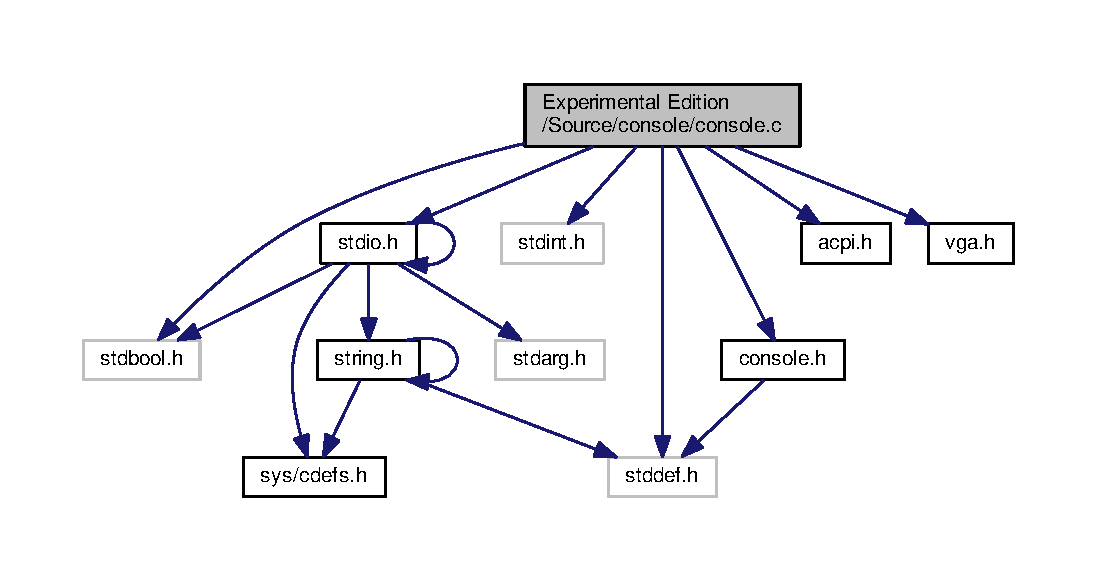
\includegraphics[width=350pt]{console_8c__incl}
\end{center}
\end{figure}
This graph shows which files directly or indirectly include this file\+:
\nopagebreak
\begin{figure}[H]
\begin{center}
\leavevmode
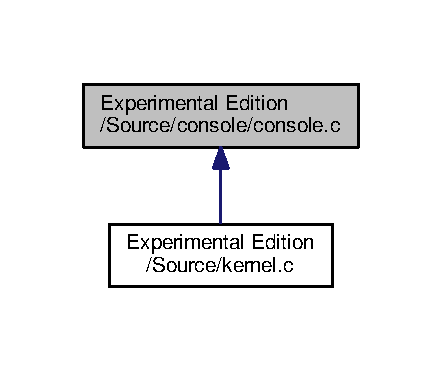
\includegraphics[width=212pt]{console_8c__dep__incl}
\end{center}
\end{figure}
\subsection*{Functions}
\begin{DoxyCompactItemize}
\item 
void \hyperlink{console_8c_acadd2a5d99d952e55a4580dbc8f8739d}{console\+\_\+init} (void)
\item 
void \hyperlink{console_8c_a7f38a80abdcd211ec9f984d50c21903a}{console\+\_\+setcolor} (uint8\+\_\+t color)
\item 
void \hyperlink{console_8c_ace5f5cd3a88b2f24cafd88827e5f6322}{console\+\_\+putentryat} (char c, uint8\+\_\+t color, size\+\_\+t x, size\+\_\+t y)
\item 
void \hyperlink{console_8c_ac156aa97dae8b45e5aea8f6534d38946}{console\+\_\+putchar} (char c)
\item 
void \hyperlink{console_8c_ad219d3a4d1adaa9323e5c3422f56f2ee}{console\+\_\+write} (const char $\ast$data, size\+\_\+t \hyperlink{multiboot_8h_a8c5ccb4d457cb24df33a7c9facfa2650}{size})
\item 
void \hyperlink{console_8c_a7e3f5006dd96b9d8c61242ddc5351832}{console\+\_\+writestring} (const char $\ast$data)
\item 
int \hyperlink{console_8c_ae8cb82b5dc7e5ff61f5610bdac37ff60}{putchar} (int ic)
\item 
void \hyperlink{console_8c_a0962a25f4eb04ccc0f0f2a1418091b35}{console\+\_\+write\+\_\+dec} (uint32\+\_\+t in)
\item 
void \hyperlink{console_8c_a4340730c5409b7e9981408c37974686d}{printint} (uint32\+\_\+t in)
\item 
void \hyperlink{console_8c_aae14f26f524b8163e88dc1d54cae9697}{backspace} ()
\end{DoxyCompactItemize}
\subsection*{Variables}
\begin{DoxyCompactItemize}
\item 
size\+\_\+t \hyperlink{console_8c_ab00bf51d192c2dcff46faf4eae44b49d}{consolerow}
\item 
size\+\_\+t \hyperlink{console_8c_a391230757710c7b1b66a5a795ff780db}{consolecolumn}
\item 
uint8\+\_\+t \hyperlink{console_8c_ad97a398a7a043a7c5896606cf2cdadf8}{console\+\_\+color}
\item 
uint16\+\_\+t $\ast$ \hyperlink{console_8c_a3776bc9cc9fb07b614fe11932150ad50}{console\+\_\+buffer}
\end{DoxyCompactItemize}


\subsection{Function Documentation}
\index{console.\+c@{console.\+c}!backspace@{backspace}}
\index{backspace@{backspace}!console.\+c@{console.\+c}}
\subsubsection[{\texorpdfstring{backspace()}{backspace()}}]{\setlength{\rightskip}{0pt plus 5cm}void backspace (
\begin{DoxyParamCaption}
{}
\end{DoxyParamCaption}
)}\hypertarget{console_8c_aae14f26f524b8163e88dc1d54cae9697}{}\label{console_8c_aae14f26f524b8163e88dc1d54cae9697}


Definition at line 144 of file console.\+c.


\begin{DoxyCode}
145 \{
146         --\hyperlink{console_8c_a391230757710c7b1b66a5a795ff780db}{consolecolumn};
147         \hyperlink{console_8c_ace5f5cd3a88b2f24cafd88827e5f6322}{console\_putentryat}(\textcolor{charliteral}{' '}, \hyperlink{console_8c_ad97a398a7a043a7c5896606cf2cdadf8}{console\_color}, 
      \hyperlink{console_8c_a391230757710c7b1b66a5a795ff780db}{consolecolumn}, \hyperlink{console_8c_ab00bf51d192c2dcff46faf4eae44b49d}{consolerow});
148 \}
\end{DoxyCode}


Here is the call graph for this function\+:
\nopagebreak
\begin{figure}[H]
\begin{center}
\leavevmode
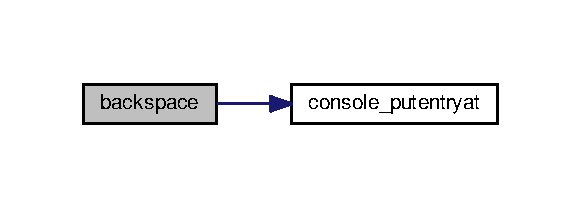
\includegraphics[width=279pt]{console_8c_aae14f26f524b8163e88dc1d54cae9697_cgraph}
\end{center}
\end{figure}


\index{console.\+c@{console.\+c}!console\+\_\+init@{console\+\_\+init}}
\index{console\+\_\+init@{console\+\_\+init}!console.\+c@{console.\+c}}
\subsubsection[{\texorpdfstring{console\+\_\+init(void)}{console_init(void)}}]{\setlength{\rightskip}{0pt plus 5cm}void console\+\_\+init (
\begin{DoxyParamCaption}
\item[{void}]{}
\end{DoxyParamCaption}
)}\hypertarget{console_8c_acadd2a5d99d952e55a4580dbc8f8739d}{}\label{console_8c_acadd2a5d99d952e55a4580dbc8f8739d}


Definition at line 15 of file console.\+c.


\begin{DoxyCode}
16 \{
17     \hyperlink{console_8c_ab00bf51d192c2dcff46faf4eae44b49d}{consolerow} = 0;
18     \hyperlink{console_8c_a391230757710c7b1b66a5a795ff780db}{consolecolumn} = 0;
19     \hyperlink{console_8c_ad97a398a7a043a7c5896606cf2cdadf8}{console\_color} = make\_color(\hyperlink{vga_8h_abaae057bae62d0c3e11501e3199cb60ea612e88bdf4015d1f208761d40c603a0e}{COLOR\_LIGHT\_GREY}, 
      \hyperlink{vga_8h_abaae057bae62d0c3e11501e3199cb60ea2a9daf215a30f1c539ead18c66380fc1}{COLOR\_BLACK});
20     \hyperlink{console_8c_a3776bc9cc9fb07b614fe11932150ad50}{console\_buffer} = VGA\_MEMORY;
21     \textcolor{keywordflow}{for} ( \textcolor{keywordtype}{size\_t} y = 0; y < VGA\_HEIGHT; y++ )
22     \{
23         \textcolor{keywordflow}{for} ( \textcolor{keywordtype}{size\_t} x = 0; x < VGA\_WIDTH; x++ )
24         \{
25             \textcolor{keyword}{const} \textcolor{keywordtype}{size\_t} index = y * VGA\_WIDTH + x;
26             \hyperlink{console_8c_a3776bc9cc9fb07b614fe11932150ad50}{console\_buffer}[index] = make\_vgaentry(\textcolor{charliteral}{' '}, 
      \hyperlink{console_8c_ad97a398a7a043a7c5896606cf2cdadf8}{console\_color});
27         \}
28     \}
29 \}
\end{DoxyCode}
\index{console.\+c@{console.\+c}!console\+\_\+putchar@{console\+\_\+putchar}}
\index{console\+\_\+putchar@{console\+\_\+putchar}!console.\+c@{console.\+c}}
\subsubsection[{\texorpdfstring{console\+\_\+putchar(char c)}{console_putchar(char c)}}]{\setlength{\rightskip}{0pt plus 5cm}void console\+\_\+putchar (
\begin{DoxyParamCaption}
\item[{char}]{c}
\end{DoxyParamCaption}
)}\hypertarget{console_8c_ac156aa97dae8b45e5aea8f6534d38946}{}\label{console_8c_ac156aa97dae8b45e5aea8f6534d38946}


Definition at line 42 of file console.\+c.


\begin{DoxyCode}
43 \{
44     \textcolor{keywordtype}{char} a=c;
45     \textcolor{keywordflow}{if}(c==\textcolor{charliteral}{'\(\backslash\)n'}) c=\textcolor{charliteral}{' '};
46     \textcolor{keywordflow}{else} \textcolor{keywordflow}{if}(c==\textcolor{charliteral}{'\(\backslash\)t'}) c=\textcolor{charliteral}{' '};
47     \hyperlink{console_8c_ace5f5cd3a88b2f24cafd88827e5f6322}{console\_putentryat}(c, \hyperlink{console_8c_ad97a398a7a043a7c5896606cf2cdadf8}{console\_color}, 
      \hyperlink{console_8c_a391230757710c7b1b66a5a795ff780db}{consolecolumn}, \hyperlink{console_8c_ab00bf51d192c2dcff46faf4eae44b49d}{consolerow});
48     \textcolor{keywordflow}{if} ( ++\hyperlink{console_8c_a391230757710c7b1b66a5a795ff780db}{consolecolumn} == VGA\_WIDTH||a==\textcolor{charliteral}{'\(\backslash\)n'})
49     \{
50         \hyperlink{console_8c_a391230757710c7b1b66a5a795ff780db}{consolecolumn} = 0;
51         \textcolor{keywordflow}{if} ( ++\hyperlink{console_8c_ab00bf51d192c2dcff46faf4eae44b49d}{consolerow} == VGA\_HEIGHT )
52         \{
53             --\hyperlink{console_8c_ab00bf51d192c2dcff46faf4eae44b49d}{consolerow};
54             uint16\_t \hyperlink{vesa_8c_af30c10a8c6ed3d4649cfdc61e2029dc3}{buff}[((VGA\_HEIGHT+1)*VGA\_WIDTH)+VGA\_WIDTH+1];
55             \textcolor{keywordflow}{for}(\textcolor{keywordtype}{size\_t} x=0;x<(((VGA\_HEIGHT+1)*VGA\_WIDTH)+VGA\_WIDTH+1);x++)
56             \{
57                 buff[x] = 0;
58             \}
59             \textcolor{keywordflow}{for} ( \textcolor{keywordtype}{size\_t} y = 0; y < VGA\_HEIGHT; y++ )
60             \{
61                 \textcolor{keywordflow}{for} ( \textcolor{keywordtype}{size\_t} x = 0; x < VGA\_WIDTH; x++ )
62                 \{
63                     \textcolor{keyword}{const} \textcolor{keywordtype}{size\_t} index = y * VGA\_WIDTH + x;
64                     buff[index] = \hyperlink{console_8c_a3776bc9cc9fb07b614fe11932150ad50}{console\_buffer}[index];
65                 \}
66             \}
67             \textcolor{keywordflow}{for} ( \textcolor{keywordtype}{size\_t} y = 0; y < VGA\_HEIGHT; y++ )
68             \{
69                 \textcolor{keywordflow}{for} ( \textcolor{keywordtype}{size\_t} x = 0; x < VGA\_WIDTH; x++ )
70                 \{
71                     \textcolor{keyword}{const} \textcolor{keywordtype}{size\_t} index = y * VGA\_WIDTH + x;
72                     \textcolor{keyword}{const} \textcolor{keywordtype}{size\_t} backindex = (y+1) * VGA\_WIDTH + x;
73                     \hyperlink{console_8c_a3776bc9cc9fb07b614fe11932150ad50}{console\_buffer}[index] = buff[backindex];
74                 \}
75             \}
76         \}
77     \}
78     \textcolor{keywordflow}{else} \textcolor{keywordflow}{if}(a==\textcolor{charliteral}{'\(\backslash\)t'})
79     \{
80         \hyperlink{console_8c_a391230757710c7b1b66a5a795ff780db}{consolecolumn}+=5;
81     \}
82 \}
\end{DoxyCode}


Here is the call graph for this function\+:
\nopagebreak
\begin{figure}[H]
\begin{center}
\leavevmode
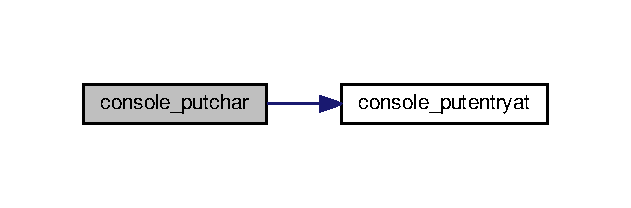
\includegraphics[width=303pt]{console_8c_ac156aa97dae8b45e5aea8f6534d38946_cgraph}
\end{center}
\end{figure}


\index{console.\+c@{console.\+c}!console\+\_\+putentryat@{console\+\_\+putentryat}}
\index{console\+\_\+putentryat@{console\+\_\+putentryat}!console.\+c@{console.\+c}}
\subsubsection[{\texorpdfstring{console\+\_\+putentryat(char c, uint8\+\_\+t color, size\+\_\+t x, size\+\_\+t y)}{console_putentryat(char c, uint8_t color, size_t x, size_t y)}}]{\setlength{\rightskip}{0pt plus 5cm}void console\+\_\+putentryat (
\begin{DoxyParamCaption}
\item[{char}]{c, }
\item[{uint8\+\_\+t}]{color, }
\item[{size\+\_\+t}]{x, }
\item[{size\+\_\+t}]{y}
\end{DoxyParamCaption}
)}\hypertarget{console_8c_ace5f5cd3a88b2f24cafd88827e5f6322}{}\label{console_8c_ace5f5cd3a88b2f24cafd88827e5f6322}


Definition at line 36 of file console.\+c.


\begin{DoxyCode}
37 \{
38     \textcolor{keyword}{const} \textcolor{keywordtype}{size\_t} index = y * VGA\_WIDTH + x;
39     \hyperlink{console_8c_a3776bc9cc9fb07b614fe11932150ad50}{console\_buffer}[index] = make\_vgaentry(c, color);
40 \}
\end{DoxyCode}
\index{console.\+c@{console.\+c}!console\+\_\+setcolor@{console\+\_\+setcolor}}
\index{console\+\_\+setcolor@{console\+\_\+setcolor}!console.\+c@{console.\+c}}
\subsubsection[{\texorpdfstring{console\+\_\+setcolor(uint8\+\_\+t color)}{console_setcolor(uint8_t color)}}]{\setlength{\rightskip}{0pt plus 5cm}void console\+\_\+setcolor (
\begin{DoxyParamCaption}
\item[{uint8\+\_\+t}]{color}
\end{DoxyParamCaption}
)}\hypertarget{console_8c_a7f38a80abdcd211ec9f984d50c21903a}{}\label{console_8c_a7f38a80abdcd211ec9f984d50c21903a}


Definition at line 31 of file console.\+c.


\begin{DoxyCode}
32 \{
33     \hyperlink{console_8c_ad97a398a7a043a7c5896606cf2cdadf8}{console\_color} = color;
34 \}
\end{DoxyCode}
\index{console.\+c@{console.\+c}!console\+\_\+write@{console\+\_\+write}}
\index{console\+\_\+write@{console\+\_\+write}!console.\+c@{console.\+c}}
\subsubsection[{\texorpdfstring{console\+\_\+write(const char $\ast$data, size\+\_\+t size)}{console_write(const char *data, size_t size)}}]{\setlength{\rightskip}{0pt plus 5cm}void console\+\_\+write (
\begin{DoxyParamCaption}
\item[{const char $\ast$}]{data, }
\item[{size\+\_\+t}]{size}
\end{DoxyParamCaption}
)}\hypertarget{console_8c_ad219d3a4d1adaa9323e5c3422f56f2ee}{}\label{console_8c_ad219d3a4d1adaa9323e5c3422f56f2ee}


Definition at line 84 of file console.\+c.


\begin{DoxyCode}
85 \{
86     \textcolor{keywordflow}{for} ( \textcolor{keywordtype}{size\_t} i = 0; i < \hyperlink{multiboot_8h_a8c5ccb4d457cb24df33a7c9facfa2650}{size}; i++ )
87         \hyperlink{console_8c_ac156aa97dae8b45e5aea8f6534d38946}{console\_putchar}(data[i]);
88 \}
\end{DoxyCode}


Here is the call graph for this function\+:
\nopagebreak
\begin{figure}[H]
\begin{center}
\leavevmode
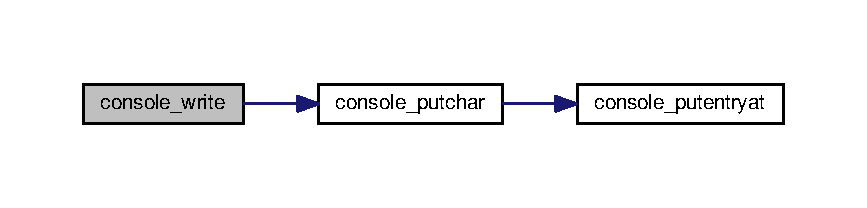
\includegraphics[width=350pt]{console_8c_ad219d3a4d1adaa9323e5c3422f56f2ee_cgraph}
\end{center}
\end{figure}


\index{console.\+c@{console.\+c}!console\+\_\+write\+\_\+dec@{console\+\_\+write\+\_\+dec}}
\index{console\+\_\+write\+\_\+dec@{console\+\_\+write\+\_\+dec}!console.\+c@{console.\+c}}
\subsubsection[{\texorpdfstring{console\+\_\+write\+\_\+dec(uint32\+\_\+t in)}{console_write_dec(uint32_t in)}}]{\setlength{\rightskip}{0pt plus 5cm}void console\+\_\+write\+\_\+dec (
\begin{DoxyParamCaption}
\item[{uint32\+\_\+t}]{in}
\end{DoxyParamCaption}
)}\hypertarget{console_8c_a0962a25f4eb04ccc0f0f2a1418091b35}{}\label{console_8c_a0962a25f4eb04ccc0f0f2a1418091b35}


Definition at line 102 of file console.\+c.


\begin{DoxyCode}
103 \{
104     uint32\_t d=1,ln=0,b=in;
105     \textcolor{keywordtype}{char} a[40];
106     \textcolor{keywordflow}{for}(uint32\_t i=0;b;i++)
107     \{
108         b=b/10;
109         ++ln;
110     \}
111     b=in;
112     \textcolor{keywordflow}{for}(uint32\_t i=0;i<ln;i++) d=d*10;
113     d=d/10;
114     uint32\_t i;
115     \textcolor{keywordflow}{for}(i=0;i<ln;i++)
116     \{
117         a[i]=48+b/d;
118         b=b%d;
119         d=d/10;
120     \}
121     a[i]=\textcolor{charliteral}{'\(\backslash\)0'};
122     \hyperlink{console_8c_a7e3f5006dd96b9d8c61242ddc5351832}{console\_writestring}(a);
123 \}
\end{DoxyCode}


Here is the call graph for this function\+:
\nopagebreak
\begin{figure}[H]
\begin{center}
\leavevmode
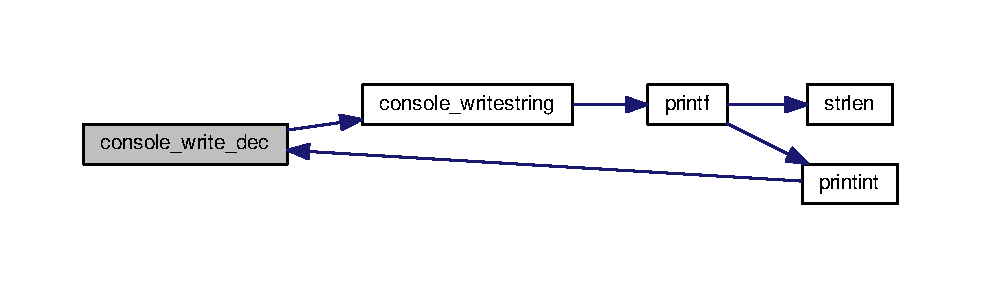
\includegraphics[width=350pt]{console_8c_a0962a25f4eb04ccc0f0f2a1418091b35_cgraph}
\end{center}
\end{figure}


\index{console.\+c@{console.\+c}!console\+\_\+writestring@{console\+\_\+writestring}}
\index{console\+\_\+writestring@{console\+\_\+writestring}!console.\+c@{console.\+c}}
\subsubsection[{\texorpdfstring{console\+\_\+writestring(const char $\ast$data)}{console_writestring(const char *data)}}]{\setlength{\rightskip}{0pt plus 5cm}void console\+\_\+writestring (
\begin{DoxyParamCaption}
\item[{const char $\ast$}]{data}
\end{DoxyParamCaption}
)}\hypertarget{console_8c_a7e3f5006dd96b9d8c61242ddc5351832}{}\label{console_8c_a7e3f5006dd96b9d8c61242ddc5351832}


Definition at line 90 of file console.\+c.


\begin{DoxyCode}
91 \{
92     \hyperlink{stdio_8h_a9eff2528601a782ae056c1b1651bb5a8}{printf}(data);
93     \textcolor{comment}{//console\_write(data, strlen(data));}
94 \}
\end{DoxyCode}


Here is the call graph for this function\+:
\nopagebreak
\begin{figure}[H]
\begin{center}
\leavevmode
\includegraphics[width=350pt]{console_8c_a7e3f5006dd96b9d8c61242ddc5351832_cgraph}
\end{center}
\end{figure}


\index{console.\+c@{console.\+c}!printint@{printint}}
\index{printint@{printint}!console.\+c@{console.\+c}}
\subsubsection[{\texorpdfstring{printint(uint32\+\_\+t in)}{printint(uint32_t in)}}]{\setlength{\rightskip}{0pt plus 5cm}void printint (
\begin{DoxyParamCaption}
\item[{uint32\+\_\+t}]{in}
\end{DoxyParamCaption}
)}\hypertarget{console_8c_a4340730c5409b7e9981408c37974686d}{}\label{console_8c_a4340730c5409b7e9981408c37974686d}


Definition at line 125 of file console.\+c.


\begin{DoxyCode}
126 \{
127     \textcolor{keywordflow}{if}(in<=999999999)
128         \hyperlink{console_8c_a0962a25f4eb04ccc0f0f2a1418091b35}{console\_write\_dec}(in);
129     \textcolor{keywordflow}{else}
130     \{
131         uint32\_t d=1,b=in,c=0;
132         \textcolor{keywordflow}{for}(uint32\_t i=0;b;i++)
133         \{
134             b=b/10;
135             ++c;
136         \}
137         c=c-9;
138         \textcolor{keywordflow}{for}(uint32\_t i=0;i<c;i++) d=d*10;
139         \hyperlink{console_8c_a0962a25f4eb04ccc0f0f2a1418091b35}{console\_write\_dec}(in/d);
140         \hyperlink{console_8c_a0962a25f4eb04ccc0f0f2a1418091b35}{console\_write\_dec}(in%d);
141     \}
142 \}
\end{DoxyCode}


Here is the call graph for this function\+:
\nopagebreak
\begin{figure}[H]
\begin{center}
\leavevmode
\includegraphics[width=350pt]{console_8c_a4340730c5409b7e9981408c37974686d_cgraph}
\end{center}
\end{figure}


\index{console.\+c@{console.\+c}!putchar@{putchar}}
\index{putchar@{putchar}!console.\+c@{console.\+c}}
\subsubsection[{\texorpdfstring{putchar(int ic)}{putchar(int ic)}}]{\setlength{\rightskip}{0pt plus 5cm}int putchar (
\begin{DoxyParamCaption}
\item[{int}]{ic}
\end{DoxyParamCaption}
)}\hypertarget{console_8c_ae8cb82b5dc7e5ff61f5610bdac37ff60}{}\label{console_8c_ae8cb82b5dc7e5ff61f5610bdac37ff60}


Definition at line 95 of file console.\+c.


\begin{DoxyCode}
96 \{
97     \textcolor{keywordtype}{char} c = (char) ic;
98     \hyperlink{console_8c_ad219d3a4d1adaa9323e5c3422f56f2ee}{console\_write}(&c, \textcolor{keyword}{sizeof}(c));
99     \textcolor{keywordflow}{return} ic;
100 \}
\end{DoxyCode}


Here is the call graph for this function\+:
\nopagebreak
\begin{figure}[H]
\begin{center}
\leavevmode
\includegraphics[width=350pt]{console_8c_ae8cb82b5dc7e5ff61f5610bdac37ff60_cgraph}
\end{center}
\end{figure}




\subsection{Variable Documentation}
\index{console.\+c@{console.\+c}!console\+\_\+buffer@{console\+\_\+buffer}}
\index{console\+\_\+buffer@{console\+\_\+buffer}!console.\+c@{console.\+c}}
\subsubsection[{\texorpdfstring{console\+\_\+buffer}{console_buffer}}]{\setlength{\rightskip}{0pt plus 5cm}uint16\+\_\+t$\ast$ console\+\_\+buffer}\hypertarget{console_8c_a3776bc9cc9fb07b614fe11932150ad50}{}\label{console_8c_a3776bc9cc9fb07b614fe11932150ad50}


Definition at line 13 of file console.\+c.

\index{console.\+c@{console.\+c}!console\+\_\+color@{console\+\_\+color}}
\index{console\+\_\+color@{console\+\_\+color}!console.\+c@{console.\+c}}
\subsubsection[{\texorpdfstring{console\+\_\+color}{console_color}}]{\setlength{\rightskip}{0pt plus 5cm}uint8\+\_\+t console\+\_\+color}\hypertarget{console_8c_ad97a398a7a043a7c5896606cf2cdadf8}{}\label{console_8c_ad97a398a7a043a7c5896606cf2cdadf8}


Definition at line 12 of file console.\+c.

\index{console.\+c@{console.\+c}!consolecolumn@{consolecolumn}}
\index{consolecolumn@{consolecolumn}!console.\+c@{console.\+c}}
\subsubsection[{\texorpdfstring{consolecolumn}{consolecolumn}}]{\setlength{\rightskip}{0pt plus 5cm}size\+\_\+t consolecolumn}\hypertarget{console_8c_a391230757710c7b1b66a5a795ff780db}{}\label{console_8c_a391230757710c7b1b66a5a795ff780db}


Definition at line 11 of file console.\+c.

\index{console.\+c@{console.\+c}!consolerow@{consolerow}}
\index{consolerow@{consolerow}!console.\+c@{console.\+c}}
\subsubsection[{\texorpdfstring{consolerow}{consolerow}}]{\setlength{\rightskip}{0pt plus 5cm}size\+\_\+t consolerow}\hypertarget{console_8c_ab00bf51d192c2dcff46faf4eae44b49d}{}\label{console_8c_ab00bf51d192c2dcff46faf4eae44b49d}


Definition at line 10 of file console.\+c.


\hypertarget{console_8h}{}\section{Experimental Edition/\+Source/console/console.h File Reference}
\label{console_8h}\index{Experimental Edition/\+Source/console/console.\+h@{Experimental Edition/\+Source/console/console.\+h}}
{\ttfamily \#include $<$stddef.\+h$>$}\\*
Include dependency graph for console.\+h\+:
\nopagebreak
\begin{figure}[H]
\begin{center}
\leavevmode
\includegraphics[width=212pt]{console_8h__incl}
\end{center}
\end{figure}
This graph shows which files directly or indirectly include this file\+:
\nopagebreak
\begin{figure}[H]
\begin{center}
\leavevmode
\includegraphics[width=350pt]{console_8h__dep__incl}
\end{center}
\end{figure}
\subsection*{Functions}
\begin{DoxyCompactItemize}
\item 
void \hyperlink{console_8h_acadd2a5d99d952e55a4580dbc8f8739d}{console\+\_\+init} (void)
\item 
void \hyperlink{console_8h_a2746e47a32f9614d1f3cacc250451c6f}{console\+\_\+putch} (char c)
\item 
void \hyperlink{console_8h_ad219d3a4d1adaa9323e5c3422f56f2ee}{console\+\_\+write} (const char $\ast$data, size\+\_\+t \hyperlink{multiboot_8h_a8c5ccb4d457cb24df33a7c9facfa2650}{size})
\item 
void \hyperlink{console_8h_a7e3f5006dd96b9d8c61242ddc5351832}{console\+\_\+writestring} (const char $\ast$data)
\item 
void \hyperlink{console_8h_aa2ad21f3a06d702a312a1182027d686c}{console\+\_\+write\+\_\+dec} (unsigned long int in)
\item 
void \hyperlink{console_8h_a3ba9e2c60586ea967a1bec1347a7d6ad}{printint} (unsigned long int in)
\item 
uint8\+\_\+t \hyperlink{console_8h_ab7981500510b079513bd93519d049b7a}{console\+\_\+manager} (char $\ast$inst)
\end{DoxyCompactItemize}
\subsection*{Variables}
\begin{DoxyCompactItemize}
\item 
void($\ast$ \hyperlink{console_8h_a0b1c810c221b3638c2afc63834428893}{mdbug} )()
\item 
void($\ast$ \hyperlink{console_8h_a84ab240c572ff018be52cc0c227ac44c}{vesa} )(uint32\+\_\+t mode)
\end{DoxyCompactItemize}


\subsection{Function Documentation}
\index{console.\+h@{console.\+h}!console\+\_\+init@{console\+\_\+init}}
\index{console\+\_\+init@{console\+\_\+init}!console.\+h@{console.\+h}}
\subsubsection[{\texorpdfstring{console\+\_\+init(void)}{console_init(void)}}]{\setlength{\rightskip}{0pt plus 5cm}void console\+\_\+init (
\begin{DoxyParamCaption}
\item[{void}]{}
\end{DoxyParamCaption}
)}\hypertarget{console_8h_acadd2a5d99d952e55a4580dbc8f8739d}{}\label{console_8h_acadd2a5d99d952e55a4580dbc8f8739d}


Definition at line 15 of file console.\+c.


\begin{DoxyCode}
16 \{
17     \hyperlink{console_8c_ab00bf51d192c2dcff46faf4eae44b49d}{consolerow} = 0;
18     \hyperlink{console_8c_a391230757710c7b1b66a5a795ff780db}{consolecolumn} = 0;
19     \hyperlink{console_8c_ad97a398a7a043a7c5896606cf2cdadf8}{console\_color} = make\_color(\hyperlink{vga_8h_abaae057bae62d0c3e11501e3199cb60ea612e88bdf4015d1f208761d40c603a0e}{COLOR\_LIGHT\_GREY}, 
      \hyperlink{vga_8h_abaae057bae62d0c3e11501e3199cb60ea2a9daf215a30f1c539ead18c66380fc1}{COLOR\_BLACK});
20     \hyperlink{console_8c_a3776bc9cc9fb07b614fe11932150ad50}{console\_buffer} = VGA\_MEMORY;
21     \textcolor{keywordflow}{for} ( \textcolor{keywordtype}{size\_t} y = 0; y < VGA\_HEIGHT; y++ )
22     \{
23         \textcolor{keywordflow}{for} ( \textcolor{keywordtype}{size\_t} x = 0; x < VGA\_WIDTH; x++ )
24         \{
25             \textcolor{keyword}{const} \textcolor{keywordtype}{size\_t} index = y * VGA\_WIDTH + x;
26             \hyperlink{console_8c_a3776bc9cc9fb07b614fe11932150ad50}{console\_buffer}[index] = make\_vgaentry(\textcolor{charliteral}{' '}, 
      \hyperlink{console_8c_ad97a398a7a043a7c5896606cf2cdadf8}{console\_color});
27         \}
28     \}
29 \}
\end{DoxyCode}
\index{console.\+h@{console.\+h}!console\+\_\+manager@{console\+\_\+manager}}
\index{console\+\_\+manager@{console\+\_\+manager}!console.\+h@{console.\+h}}
\subsubsection[{\texorpdfstring{console\+\_\+manager(char $\ast$inst)}{console_manager(char *inst)}}]{\setlength{\rightskip}{0pt plus 5cm}uint8\+\_\+t console\+\_\+manager (
\begin{DoxyParamCaption}
\item[{char $\ast$}]{inst}
\end{DoxyParamCaption}
)}\hypertarget{console_8h_ab7981500510b079513bd93519d049b7a}{}\label{console_8h_ab7981500510b079513bd93519d049b7a}


Definition at line 194 of file kernel.\+c.


\begin{DoxyCode}
195 \{
196     \textcolor{keywordflow}{if}(!\hyperlink{string_8h_a34624c3be7459f677d90ae0ad046821a}{strcmp}(inst,\textcolor{stringliteral}{"help"}))
197     \{
198         \hyperlink{stdio_8h_a9eff2528601a782ae056c1b1651bb5a8}{printf}(\textcolor{stringliteral}{"\(\backslash\)nAvialable Commands are:\(\backslash\)n"});
199         \hyperlink{stdio_8h_a9eff2528601a782ae056c1b1651bb5a8}{printf}(\textcolor{stringliteral}{"\(\backslash\)n\(\backslash\)thelp         To get all the available commands"});
200         \hyperlink{stdio_8h_a9eff2528601a782ae056c1b1651bb5a8}{printf}(\textcolor{stringliteral}{"\(\backslash\)n\(\backslash\)tmdbug        To test the Memory Managment System"});
201         \hyperlink{stdio_8h_a9eff2528601a782ae056c1b1651bb5a8}{printf}(\textcolor{stringliteral}{"\(\backslash\)n\(\backslash\)tshutdown     To ACPI Power off the system (may not work on few machines)"});
202         \hyperlink{stdio_8h_a9eff2528601a782ae056c1b1651bb5a8}{printf}(\textcolor{stringliteral}{"\(\backslash\)n\(\backslash\)tstart vesa   To enter VESA Super VGA Mode"});
203         \hyperlink{stdio_8h_a9eff2528601a782ae056c1b1651bb5a8}{printf}(\textcolor{stringliteral}{"\(\backslash\)n\(\backslash\)tmemmap       To view the Physical Memory Map of the system"});
204         \hyperlink{stdio_8h_a9eff2528601a782ae056c1b1651bb5a8}{printf}(\textcolor{stringliteral}{"\(\backslash\)n\(\backslash\)ttest multi   To Test multitasking"});
205         \hyperlink{stdio_8h_a9eff2528601a782ae056c1b1651bb5a8}{printf}(\textcolor{stringliteral}{"\(\backslash\)n\(\backslash\)tother commands\(\backslash\)n"});
206         \textcolor{keywordflow}{return} 0;
207     \}
208     \textcolor{keywordflow}{else} \textcolor{keywordflow}{if}(!\hyperlink{string_8h_a34624c3be7459f677d90ae0ad046821a}{strcmp}(inst,\textcolor{stringliteral}{"shutdown"}))
209     \{
210             \hyperlink{stdio_8h_a9eff2528601a782ae056c1b1651bb5a8}{printf}(\textcolor{stringliteral}{"\(\backslash\)n Turning Power off"});
211             \hyperlink{acpi_8c_a6f63c2b70d3c6d268bdc2423d3fdfb9f}{acpiPowerOff}();
212             \textcolor{keywordflow}{return} 0;
213     \}
214     \textcolor{keywordflow}{else} \textcolor{keywordflow}{if}(!\hyperlink{string_8h_a34624c3be7459f677d90ae0ad046821a}{strcmp}(inst,\textcolor{stringliteral}{"mdbug"}))
215     \{
216             \hyperlink{stdio_8h_a9eff2528601a782ae056c1b1651bb5a8}{printf}(\textcolor{stringliteral}{"\(\backslash\)n Testing Virtual Memory Manager"});
217             \hyperlink{console_8h_a0b1c810c221b3638c2afc63834428893}{mdbug}();
218             \textcolor{keywordflow}{return} 0;
219     \}
220     \textcolor{keywordflow}{else} \textcolor{keywordflow}{if}(!\hyperlink{string_8h_a34624c3be7459f677d90ae0ad046821a}{strcmp}(inst,\textcolor{stringliteral}{"start vesa"}))
221     \{
222         \hyperlink{stdio_8h_a9eff2528601a782ae056c1b1651bb5a8}{printf}(\textcolor{stringliteral}{"\(\backslash\)n Entering VESA SVGA mode 1024*768"});
223         \hyperlink{console_8h_a84ab240c572ff018be52cc0c227ac44c}{vesa}(0x117);
224         \textcolor{keywordflow}{return} 1;
225     \}
226     \textcolor{keywordflow}{else} \textcolor{keywordflow}{if}(!\hyperlink{string_8h_a34624c3be7459f677d90ae0ad046821a}{strcmp}(inst,\textcolor{stringliteral}{"memmap"}))
227     \{
228     \hyperlink{stdio_8h_a9eff2528601a782ae056c1b1651bb5a8}{printf}(\textcolor{stringliteral}{"\(\backslash\)nMemory Map:"});
229     \hyperlink{structmemory__region}{MemRegion\_t}* memmap\_info=\hyperlink{vmem_8h_a652241438a84d50f059167c4eea7f1cc}{mmap\_info};
230 
231     \textcolor{keywordflow}{for}(\textcolor{keywordtype}{int} i=0;i<15;i++)
232     \{
233         \textcolor{keywordflow}{if}(memmap\_info->\hyperlink{structmemory__region_a85b8ec619e9aa2053ea033c5b7d3683c}{startLo}==0) \textcolor{keywordflow}{break};
234         \hyperlink{stdio_8h_a9eff2528601a782ae056c1b1651bb5a8}{printf}(\textcolor{stringliteral}{"region %i address: %x size: %x Bytes Type: %i (%s)\(\backslash\)n"},i,memmap\_info->
      \hyperlink{structmemory__region_a090957a0a7f28700a605cf6f5e8f614a}{startHi},memmap\_info->\hyperlink{structmemory__region_a3d6aa91c428379cfc829556e48aee067}{sizeHi},
235                memmap\_info->\hyperlink{structmemory__region_a3591afc4df88a58fa5a91eab6ebe94cc}{type},\hyperlink{vmem_8h_aa980b4f0db6827466a011796b1179f71}{strMemoryTypes}[memmap\_info->
      \hyperlink{structmemory__region_a3591afc4df88a58fa5a91eab6ebe94cc}{type}-1]);
236         memmap\_info++;
237     \}
238         \textcolor{keywordflow}{return} 0;
239     \}
240     \textcolor{keywordflow}{else} \textcolor{keywordflow}{if}(!\hyperlink{string_8h_a34624c3be7459f677d90ae0ad046821a}{strcmp}(inst,\textcolor{stringliteral}{"test multi"}))
241     \{
242         \textcolor{comment}{//schedule=switch\_task;}
243         \textcolor{comment}{//printf("\(\backslash\)n\(\backslash\)tEnter the timer Value:");}
244         \textcolor{comment}{//uint32\_t timer=getint();}
245         \hyperlink{task_8c_aa84eaf17b807dd55decb63a2de5f1bc7}{Scheduler\_exec}();
246         \textcolor{keywordflow}{return} 0;
247     \}
248     \textcolor{keywordflow}{else} \textcolor{keywordflow}{if}(!\hyperlink{string_8h_a34624c3be7459f677d90ae0ad046821a}{strcmp}(inst,\textcolor{stringliteral}{"rand-gen"}))
249     \{
250         \hyperlink{task_8c_aed5860394b06605b9c6de6e8a31f74fa}{rand\_test}();
251         \textcolor{keywordflow}{return} 0;
252     \}
253     \hyperlink{stdio_8h_a9eff2528601a782ae056c1b1651bb5a8}{printf}(\textcolor{stringliteral}{"\(\backslash\)n Command Not Recognized! type help for help\(\backslash\)n"});
254     \textcolor{keywordflow}{return} 0;
255 \}
\end{DoxyCode}


Here is the call graph for this function\+:
\nopagebreak
\begin{figure}[H]
\begin{center}
\leavevmode
\includegraphics[width=350pt]{console_8h_ab7981500510b079513bd93519d049b7a_cgraph}
\end{center}
\end{figure}


\index{console.\+h@{console.\+h}!console\+\_\+putch@{console\+\_\+putch}}
\index{console\+\_\+putch@{console\+\_\+putch}!console.\+h@{console.\+h}}
\subsubsection[{\texorpdfstring{console\+\_\+putch(char c)}{console_putch(char c)}}]{\setlength{\rightskip}{0pt plus 5cm}void console\+\_\+putch (
\begin{DoxyParamCaption}
\item[{char}]{c}
\end{DoxyParamCaption}
)}\hypertarget{console_8h_a2746e47a32f9614d1f3cacc250451c6f}{}\label{console_8h_a2746e47a32f9614d1f3cacc250451c6f}
\index{console.\+h@{console.\+h}!console\+\_\+write@{console\+\_\+write}}
\index{console\+\_\+write@{console\+\_\+write}!console.\+h@{console.\+h}}
\subsubsection[{\texorpdfstring{console\+\_\+write(const char $\ast$data, size\+\_\+t size)}{console_write(const char *data, size_t size)}}]{\setlength{\rightskip}{0pt plus 5cm}void console\+\_\+write (
\begin{DoxyParamCaption}
\item[{const char $\ast$}]{data, }
\item[{size\+\_\+t}]{size}
\end{DoxyParamCaption}
)}\hypertarget{console_8h_ad219d3a4d1adaa9323e5c3422f56f2ee}{}\label{console_8h_ad219d3a4d1adaa9323e5c3422f56f2ee}


Definition at line 84 of file console.\+c.


\begin{DoxyCode}
85 \{
86     \textcolor{keywordflow}{for} ( \textcolor{keywordtype}{size\_t} i = 0; i < \hyperlink{multiboot_8h_a8c5ccb4d457cb24df33a7c9facfa2650}{size}; i++ )
87         \hyperlink{console_8c_ac156aa97dae8b45e5aea8f6534d38946}{console\_putchar}(data[i]);
88 \}
\end{DoxyCode}


Here is the call graph for this function\+:
\nopagebreak
\begin{figure}[H]
\begin{center}
\leavevmode
\includegraphics[width=350pt]{console_8h_ad219d3a4d1adaa9323e5c3422f56f2ee_cgraph}
\end{center}
\end{figure}


\index{console.\+h@{console.\+h}!console\+\_\+write\+\_\+dec@{console\+\_\+write\+\_\+dec}}
\index{console\+\_\+write\+\_\+dec@{console\+\_\+write\+\_\+dec}!console.\+h@{console.\+h}}
\subsubsection[{\texorpdfstring{console\+\_\+write\+\_\+dec(unsigned long int in)}{console_write_dec(unsigned long int in)}}]{\setlength{\rightskip}{0pt plus 5cm}void console\+\_\+write\+\_\+dec (
\begin{DoxyParamCaption}
\item[{unsigned long int}]{in}
\end{DoxyParamCaption}
)}\hypertarget{console_8h_aa2ad21f3a06d702a312a1182027d686c}{}\label{console_8h_aa2ad21f3a06d702a312a1182027d686c}
\index{console.\+h@{console.\+h}!console\+\_\+writestring@{console\+\_\+writestring}}
\index{console\+\_\+writestring@{console\+\_\+writestring}!console.\+h@{console.\+h}}
\subsubsection[{\texorpdfstring{console\+\_\+writestring(const char $\ast$data)}{console_writestring(const char *data)}}]{\setlength{\rightskip}{0pt plus 5cm}void console\+\_\+writestring (
\begin{DoxyParamCaption}
\item[{const char $\ast$}]{data}
\end{DoxyParamCaption}
)}\hypertarget{console_8h_a7e3f5006dd96b9d8c61242ddc5351832}{}\label{console_8h_a7e3f5006dd96b9d8c61242ddc5351832}


Definition at line 90 of file console.\+c.


\begin{DoxyCode}
91 \{
92     \hyperlink{stdio_8h_a9eff2528601a782ae056c1b1651bb5a8}{printf}(data);
93     \textcolor{comment}{//console\_write(data, strlen(data));}
94 \}
\end{DoxyCode}


Here is the call graph for this function\+:
\nopagebreak
\begin{figure}[H]
\begin{center}
\leavevmode
\includegraphics[width=350pt]{console_8h_a7e3f5006dd96b9d8c61242ddc5351832_cgraph}
\end{center}
\end{figure}


\index{console.\+h@{console.\+h}!printint@{printint}}
\index{printint@{printint}!console.\+h@{console.\+h}}
\subsubsection[{\texorpdfstring{printint(unsigned long int in)}{printint(unsigned long int in)}}]{\setlength{\rightskip}{0pt plus 5cm}void printint (
\begin{DoxyParamCaption}
\item[{unsigned long int}]{in}
\end{DoxyParamCaption}
)}\hypertarget{console_8h_a3ba9e2c60586ea967a1bec1347a7d6ad}{}\label{console_8h_a3ba9e2c60586ea967a1bec1347a7d6ad}


\subsection{Variable Documentation}
\index{console.\+h@{console.\+h}!mdbug@{mdbug}}
\index{mdbug@{mdbug}!console.\+h@{console.\+h}}
\subsubsection[{\texorpdfstring{mdbug}{mdbug}}]{\setlength{\rightskip}{0pt plus 5cm}void($\ast$ mdbug) ()}\hypertarget{console_8h_a0b1c810c221b3638c2afc63834428893}{}\label{console_8h_a0b1c810c221b3638c2afc63834428893}


Definition at line 4 of file console.\+h.

\index{console.\+h@{console.\+h}!vesa@{vesa}}
\index{vesa@{vesa}!console.\+h@{console.\+h}}
\subsubsection[{\texorpdfstring{vesa}{vesa}}]{\setlength{\rightskip}{0pt plus 5cm}void($\ast$ vesa) (uint32\+\_\+t mode)}\hypertarget{console_8h_a84ab240c572ff018be52cc0c227ac44c}{}\label{console_8h_a84ab240c572ff018be52cc0c227ac44c}


Definition at line 5 of file console.\+h.


\hypertarget{acpi_8c}{}\section{Experimental Edition/\+Source/\+Drivers/\+A\+C\+P\+I/acpi.c File Reference}
\label{acpi_8c}\index{Experimental Edition/\+Source/\+Drivers/\+A\+C\+P\+I/acpi.\+c@{Experimental Edition/\+Source/\+Drivers/\+A\+C\+P\+I/acpi.\+c}}
{\ttfamily \#include $<$stddef.\+h$>$}\\*
{\ttfamily \#include $<$console.\+h$>$}\\*
{\ttfamily \#include $<$string.\+h$>$}\\*
{\ttfamily \#include $<$sys.\+h$>$}\\*
{\ttfamily \#include $<$system.\+h$>$}\\*
Include dependency graph for acpi.\+c\+:
\nopagebreak
\begin{figure}[H]
\begin{center}
\leavevmode
\includegraphics[width=350pt]{acpi_8c__incl}
\end{center}
\end{figure}
This graph shows which files directly or indirectly include this file\+:
\nopagebreak
\begin{figure}[H]
\begin{center}
\leavevmode
\includegraphics[width=192pt]{acpi_8c__dep__incl}
\end{center}
\end{figure}
\subsection*{Data Structures}
\begin{DoxyCompactItemize}
\item 
struct \hyperlink{structRSDPtr}{R\+S\+D\+Ptr}
\item 
struct \hyperlink{structFACP}{F\+A\+CP}
\end{DoxyCompactItemize}
\subsection*{Typedefs}
\begin{DoxyCompactItemize}
\item 
typedef unsigned char \hyperlink{acpi_8c_a0c8186d9b9b7880309c27230bbb5e69d}{byte}
\item 
typedef unsigned short \hyperlink{acpi_8c_a285e72252c100e2508e4e933a0738f2b}{word}
\item 
typedef unsigned long \hyperlink{acpi_8c_a74cb93d430006e784da73b8ca406ee6e}{dword}
\item 
typedef unsigned int \hyperlink{acpi_8c_a97e9b18a159dda578a4e92c8c5634633}{qword}
\end{DoxyCompactItemize}
\subsection*{Functions}
\begin{DoxyCompactItemize}
\item 
unsigned int $\ast$ \hyperlink{acpi_8c_ac6e4f33d3233a13cacc16cb3b4a1b00d}{acpi\+Check\+R\+S\+D\+Ptr} (unsigned int $\ast$ptr)
\item 
unsigned int $\ast$ \hyperlink{acpi_8c_a6ea46d1e05611b3b6a689777fe4a23c3}{acpi\+Get\+R\+S\+D\+Ptr} (void)
\item 
int \hyperlink{acpi_8c_ae00c7f44d9e3e3bedcc4b43425788c43}{acpi\+Check\+Header} (unsigned int $\ast$ptr, char $\ast$sig)
\item 
int \hyperlink{acpi_8c_a7785e47ec7c5a61c43890af2581da359}{acpi\+Enable} (void)
\item 
int \hyperlink{acpi_8c_a7fe73cf42200ac2245d5dd48fe2268db}{init\+Acpi} (void)
\item 
void \hyperlink{acpi_8c_a6f63c2b70d3c6d268bdc2423d3fdfb9f}{acpi\+Power\+Off} (void)
\end{DoxyCompactItemize}
\subsection*{Variables}
\begin{DoxyCompactItemize}
\item 
\hyperlink{acpi_8c_a74cb93d430006e784da73b8ca406ee6e}{dword} $\ast$ \hyperlink{acpi_8c_a33b8ab25b3f4c51863b154877144f3df}{S\+M\+I\+\_\+\+C\+MD}
\item 
\hyperlink{acpi_8c_a0c8186d9b9b7880309c27230bbb5e69d}{byte} \hyperlink{acpi_8c_a34153f28c481147d24e470eb95db14ea}{A\+C\+P\+I\+\_\+\+E\+N\+A\+B\+LE}
\item 
\hyperlink{acpi_8c_a0c8186d9b9b7880309c27230bbb5e69d}{byte} \hyperlink{acpi_8c_a03d9362da0e66c33d75b9a3249255158}{A\+C\+P\+I\+\_\+\+D\+I\+S\+A\+B\+LE}
\item 
\hyperlink{acpi_8c_a74cb93d430006e784da73b8ca406ee6e}{dword} $\ast$ \hyperlink{acpi_8c_a1a546c2755013ff60aaafcdab0befae9}{P\+M1a\+\_\+\+C\+NT}
\item 
\hyperlink{acpi_8c_a74cb93d430006e784da73b8ca406ee6e}{dword} $\ast$ \hyperlink{acpi_8c_a58d7d7d0ab171e520fae96b370db740b}{P\+M1b\+\_\+\+C\+NT}
\item 
\hyperlink{acpi_8c_a285e72252c100e2508e4e933a0738f2b}{word} \hyperlink{acpi_8c_a377b954bbafc1caae62c790a84625e2c}{S\+L\+P\+\_\+\+T\+Y\+Pa}
\item 
\hyperlink{acpi_8c_a285e72252c100e2508e4e933a0738f2b}{word} \hyperlink{acpi_8c_a73d59c76364473fa8dfb23f609728568}{S\+L\+P\+\_\+\+T\+Y\+Pb}
\item 
\hyperlink{acpi_8c_a285e72252c100e2508e4e933a0738f2b}{word} \hyperlink{acpi_8c_a865638a43175e3591eb2c085ffd21317}{S\+L\+P\+\_\+\+EN}
\item 
\hyperlink{acpi_8c_a285e72252c100e2508e4e933a0738f2b}{word} \hyperlink{acpi_8c_a15c1e5908be89bca113b617faa86b6f3}{S\+C\+I\+\_\+\+EN}
\item 
\hyperlink{acpi_8c_a0c8186d9b9b7880309c27230bbb5e69d}{byte} \hyperlink{acpi_8c_a1a17515f9c86fc1266c1f04b7c5eb10e}{P\+M1\+\_\+\+C\+N\+T\+\_\+\+L\+EN}
\end{DoxyCompactItemize}


\subsection{Typedef Documentation}
\index{acpi.\+c@{acpi.\+c}!byte@{byte}}
\index{byte@{byte}!acpi.\+c@{acpi.\+c}}
\subsubsection[{\texorpdfstring{byte}{byte}}]{\setlength{\rightskip}{0pt plus 5cm}typedef unsigned char {\bf byte}}\hypertarget{acpi_8c_a0c8186d9b9b7880309c27230bbb5e69d}{}\label{acpi_8c_a0c8186d9b9b7880309c27230bbb5e69d}


Definition at line 7 of file acpi.\+c.

\index{acpi.\+c@{acpi.\+c}!dword@{dword}}
\index{dword@{dword}!acpi.\+c@{acpi.\+c}}
\subsubsection[{\texorpdfstring{dword}{dword}}]{\setlength{\rightskip}{0pt plus 5cm}typedef unsigned long {\bf dword}}\hypertarget{acpi_8c_a74cb93d430006e784da73b8ca406ee6e}{}\label{acpi_8c_a74cb93d430006e784da73b8ca406ee6e}


Definition at line 9 of file acpi.\+c.

\index{acpi.\+c@{acpi.\+c}!qword@{qword}}
\index{qword@{qword}!acpi.\+c@{acpi.\+c}}
\subsubsection[{\texorpdfstring{qword}{qword}}]{\setlength{\rightskip}{0pt plus 5cm}typedef unsigned int {\bf qword}}\hypertarget{acpi_8c_a97e9b18a159dda578a4e92c8c5634633}{}\label{acpi_8c_a97e9b18a159dda578a4e92c8c5634633}


Definition at line 10 of file acpi.\+c.

\index{acpi.\+c@{acpi.\+c}!word@{word}}
\index{word@{word}!acpi.\+c@{acpi.\+c}}
\subsubsection[{\texorpdfstring{word}{word}}]{\setlength{\rightskip}{0pt plus 5cm}typedef unsigned short {\bf word}}\hypertarget{acpi_8c_a285e72252c100e2508e4e933a0738f2b}{}\label{acpi_8c_a285e72252c100e2508e4e933a0738f2b}


Definition at line 8 of file acpi.\+c.



\subsection{Function Documentation}
\index{acpi.\+c@{acpi.\+c}!acpi\+Check\+Header@{acpi\+Check\+Header}}
\index{acpi\+Check\+Header@{acpi\+Check\+Header}!acpi.\+c@{acpi.\+c}}
\subsubsection[{\texorpdfstring{acpi\+Check\+Header(unsigned int $\ast$ptr, char $\ast$sig)}{acpiCheckHeader(unsigned int *ptr, char *sig)}}]{\setlength{\rightskip}{0pt plus 5cm}int acpi\+Check\+Header (
\begin{DoxyParamCaption}
\item[{unsigned int $\ast$}]{ptr, }
\item[{char $\ast$}]{sig}
\end{DoxyParamCaption}
)}\hypertarget{acpi_8c_ae00c7f44d9e3e3bedcc4b43425788c43}{}\label{acpi_8c_ae00c7f44d9e3e3bedcc4b43425788c43}


Definition at line 124 of file acpi.\+c.


\begin{DoxyCode}
125 \{
126    \textcolor{keywordflow}{if} (\hyperlink{string_8h_a3376078c105a2293e911a180e7fbab4b}{memcmp}(ptr, sig, 4) == 0)
127    \{
128       \textcolor{keywordtype}{char} *checkPtr = (\textcolor{keywordtype}{char} *) ptr;
129       \textcolor{keywordtype}{int} len = *(ptr + 1);
130       \textcolor{keywordtype}{char} check = 0;
131       \textcolor{keywordflow}{while} (0<len--)
132       \{
133          check += *checkPtr;
134          checkPtr++;
135       \}
136       \textcolor{keywordflow}{if} (check == 0)
137          \textcolor{keywordflow}{return} 0;
138    \}
139    \textcolor{keywordflow}{return} -1;
140 \}
\end{DoxyCode}


Here is the call graph for this function\+:
\nopagebreak
\begin{figure}[H]
\begin{center}
\leavevmode
\includegraphics[width=268pt]{acpi_8c_ae00c7f44d9e3e3bedcc4b43425788c43_cgraph}
\end{center}
\end{figure}


\index{acpi.\+c@{acpi.\+c}!acpi\+Check\+R\+S\+D\+Ptr@{acpi\+Check\+R\+S\+D\+Ptr}}
\index{acpi\+Check\+R\+S\+D\+Ptr@{acpi\+Check\+R\+S\+D\+Ptr}!acpi.\+c@{acpi.\+c}}
\subsubsection[{\texorpdfstring{acpi\+Check\+R\+S\+D\+Ptr(unsigned int $\ast$ptr)}{acpiCheckRSDPtr(unsigned int *ptr)}}]{\setlength{\rightskip}{0pt plus 5cm}unsigned int$\ast$ acpi\+Check\+R\+S\+D\+Ptr (
\begin{DoxyParamCaption}
\item[{unsigned int $\ast$}]{ptr}
\end{DoxyParamCaption}
)}\hypertarget{acpi_8c_ac6e4f33d3233a13cacc16cb3b4a1b00d}{}\label{acpi_8c_ac6e4f33d3233a13cacc16cb3b4a1b00d}


Definition at line 56 of file acpi.\+c.


\begin{DoxyCode}
57 \{
58    \textcolor{keywordtype}{char} *sig = \textcolor{stringliteral}{"RSD PTR "};
59    \textcolor{keyword}{struct }\hyperlink{structRSDPtr}{RSDPtr} *rsdp = (\textcolor{keyword}{struct }\hyperlink{structRSDPtr}{RSDPtr} *) ptr;
60    \hyperlink{acpi_8c_a0c8186d9b9b7880309c27230bbb5e69d}{byte} *bptr;
61    \hyperlink{acpi_8c_a0c8186d9b9b7880309c27230bbb5e69d}{byte} check = 0;
62    uint32\_t i;
63 
64    \textcolor{keywordflow}{if} (\hyperlink{string_8h_a3376078c105a2293e911a180e7fbab4b}{memcmp}(sig, rsdp, 8) == 0)
65    \{
66       \textcolor{comment}{// check checksum rsdpd}
67       bptr = (\hyperlink{acpi_8c_a0c8186d9b9b7880309c27230bbb5e69d}{byte} *) ptr;
68       \textcolor{keywordflow}{for} (i=0; i<\textcolor{keyword}{sizeof}(\textcolor{keyword}{struct }\hyperlink{structRSDPtr}{RSDPtr}); i++)
69       \{
70          check += *bptr;
71          bptr++;
72       \}
73 
74       \textcolor{comment}{// found valid rsdpd}
75       \textcolor{keywordflow}{if} (check == 0) \{
76          \textcolor{comment}{/*}
77 \textcolor{comment}{          if (desc->Revision == 0)}
78 \textcolor{comment}{            wrstr("acpi 1");}
79 \textcolor{comment}{         else}
80 \textcolor{comment}{            wrstr("acpi 2");}
81 \textcolor{comment}{         */}
82          \textcolor{keywordflow}{return} (\textcolor{keywordtype}{unsigned} \textcolor{keywordtype}{int} *) rsdp->\hyperlink{structRSDPtr_a982825bea34910320148af4114ba8e00}{RsdtAddress};
83       \}
84    \}
85 
86    \textcolor{keywordflow}{return} \hyperlink{common_8h_a070d2ce7b6bb7e5c05602aa8c308d0c4}{NULL};
87 \}
\end{DoxyCode}


Here is the call graph for this function\+:
\nopagebreak
\begin{figure}[H]
\begin{center}
\leavevmode
\includegraphics[width=271pt]{acpi_8c_ac6e4f33d3233a13cacc16cb3b4a1b00d_cgraph}
\end{center}
\end{figure}


\index{acpi.\+c@{acpi.\+c}!acpi\+Enable@{acpi\+Enable}}
\index{acpi\+Enable@{acpi\+Enable}!acpi.\+c@{acpi.\+c}}
\subsubsection[{\texorpdfstring{acpi\+Enable(void)}{acpiEnable(void)}}]{\setlength{\rightskip}{0pt plus 5cm}int acpi\+Enable (
\begin{DoxyParamCaption}
\item[{void}]{}
\end{DoxyParamCaption}
)}\hypertarget{acpi_8c_a7785e47ec7c5a61c43890af2581da359}{}\label{acpi_8c_a7785e47ec7c5a61c43890af2581da359}


Definition at line 144 of file acpi.\+c.


\begin{DoxyCode}
145 \{
146    \textcolor{comment}{// check if acpi is enabled}
147    \textcolor{keywordflow}{if} ( (\hyperlink{sys_8h_a3dcbb9e13203beb0e38956999e8ae61d}{inw}((\textcolor{keywordtype}{unsigned} \textcolor{keywordtype}{int}) \hyperlink{acpi_8c_a1a546c2755013ff60aaafcdab0befae9}{PM1a\_CNT}) &\hyperlink{acpi_8c_a15c1e5908be89bca113b617faa86b6f3}{SCI\_EN}) == 0 )
148    \{
149       \textcolor{comment}{// check if acpi can be enabled}
150       \textcolor{keywordflow}{if} (\hyperlink{acpi_8c_a33b8ab25b3f4c51863b154877144f3df}{SMI\_CMD} != 0 && \hyperlink{acpi_8c_a34153f28c481147d24e470eb95db14ea}{ACPI\_ENABLE} != 0)
151       \{
152          \hyperlink{sys_8h_a1fe613f83e149aa1a4ae0d5f5149ab34}{outb}((\textcolor{keywordtype}{unsigned} \textcolor{keywordtype}{int}) \hyperlink{acpi_8c_a33b8ab25b3f4c51863b154877144f3df}{SMI\_CMD}, \hyperlink{acpi_8c_a34153f28c481147d24e470eb95db14ea}{ACPI\_ENABLE}); \textcolor{comment}{// send acpi enable command}
153          \textcolor{comment}{// give 3 seconds time to enable acpi}
154          \textcolor{keywordtype}{int} i;
155          \textcolor{keywordflow}{for} (i=0; i<300; i++ )
156          \{
157             \textcolor{keywordflow}{if} ( (\hyperlink{sys_8h_a3dcbb9e13203beb0e38956999e8ae61d}{inw}((\textcolor{keywordtype}{unsigned} \textcolor{keywordtype}{int}) PM1a\_CNT) &SCI\_EN) == 1 )
158                \textcolor{keywordflow}{break};
159             \hyperlink{ata_8c_ab24cd262423caf1599380572e83824fa}{sleep}(10);
160          \}
161          \textcolor{keywordflow}{if} (\hyperlink{acpi_8c_a58d7d7d0ab171e520fae96b370db740b}{PM1b\_CNT} != 0)
162             \textcolor{keywordflow}{for} (; i<300; i++ )
163             \{
164                \textcolor{keywordflow}{if} ( (\hyperlink{sys_8h_a3dcbb9e13203beb0e38956999e8ae61d}{inw}((\textcolor{keywordtype}{unsigned} \textcolor{keywordtype}{int}) \hyperlink{acpi_8c_a58d7d7d0ab171e520fae96b370db740b}{PM1b\_CNT}) &SCI\_EN) == 1 )
165                   \textcolor{keywordflow}{break};
166                \hyperlink{ata_8c_ab24cd262423caf1599380572e83824fa}{sleep}(10);
167             \}
168          \textcolor{keywordflow}{if} (i<300) \{
169             \hyperlink{console_8c_a7e3f5006dd96b9d8c61242ddc5351832}{console\_writestring}(\textcolor{stringliteral}{"enabled acpi.\(\backslash\)n"});
170             \textcolor{keywordflow}{return} 0;
171          \} \textcolor{keywordflow}{else} \{
172             \hyperlink{console_8c_a7e3f5006dd96b9d8c61242ddc5351832}{console\_writestring}(\textcolor{stringliteral}{"couldn't enable acpi.\(\backslash\)n"});
173             \textcolor{keywordflow}{return} -1;
174          \}
175       \} \textcolor{keywordflow}{else} \{
176          \hyperlink{console_8c_a7e3f5006dd96b9d8c61242ddc5351832}{console\_writestring}(\textcolor{stringliteral}{"no known way to enable acpi.\(\backslash\)n"});
177          \textcolor{keywordflow}{return} -1;
178       \}
179    \} \textcolor{keywordflow}{else} \{
180       \textcolor{comment}{//wrstr("acpi was already enabled.\(\backslash\)n");}
181       \textcolor{keywordflow}{return} 0;
182    \}
183 \}
\end{DoxyCode}


Here is the call graph for this function\+:
\nopagebreak
\begin{figure}[H]
\begin{center}
\leavevmode
\includegraphics[width=350pt]{acpi_8c_a7785e47ec7c5a61c43890af2581da359_cgraph}
\end{center}
\end{figure}


\index{acpi.\+c@{acpi.\+c}!acpi\+Get\+R\+S\+D\+Ptr@{acpi\+Get\+R\+S\+D\+Ptr}}
\index{acpi\+Get\+R\+S\+D\+Ptr@{acpi\+Get\+R\+S\+D\+Ptr}!acpi.\+c@{acpi.\+c}}
\subsubsection[{\texorpdfstring{acpi\+Get\+R\+S\+D\+Ptr(void)}{acpiGetRSDPtr(void)}}]{\setlength{\rightskip}{0pt plus 5cm}unsigned int$\ast$ acpi\+Get\+R\+S\+D\+Ptr (
\begin{DoxyParamCaption}
\item[{void}]{}
\end{DoxyParamCaption}
)}\hypertarget{acpi_8c_a6ea46d1e05611b3b6a689777fe4a23c3}{}\label{acpi_8c_a6ea46d1e05611b3b6a689777fe4a23c3}


Definition at line 92 of file acpi.\+c.


\begin{DoxyCode}
93 \{
94    \textcolor{keywordtype}{unsigned} \textcolor{keywordtype}{int} *\hyperlink{multiboot_8h_a48f994dfe1a5aea3bce6dc7d2be8efd5}{addr};
95    \textcolor{keywordtype}{unsigned} \textcolor{keywordtype}{int} *rsdp;
96 
97    \textcolor{comment}{// search below the 1mb mark for RSDP signature}
98    \textcolor{keywordflow}{for} (addr = (\textcolor{keywordtype}{unsigned} \textcolor{keywordtype}{int} *) 0x000E0000; (int) addr<0x00100000; addr += 0x10/\textcolor{keyword}{sizeof}(
      \hyperlink{multiboot_8h_a48f994dfe1a5aea3bce6dc7d2be8efd5}{addr}))
99    \{
100       rsdp = \hyperlink{acpi_8c_ac6e4f33d3233a13cacc16cb3b4a1b00d}{acpiCheckRSDPtr}(addr);
101       \textcolor{keywordflow}{if} (rsdp != \hyperlink{common_8h_a070d2ce7b6bb7e5c05602aa8c308d0c4}{NULL})
102          \textcolor{keywordflow}{return} rsdp;
103    \}
104 
105 
106    \textcolor{comment}{// at address 0x40:0x0E is the RM segment of the ebda}
107    \textcolor{keywordtype}{int} ebda = *((\textcolor{keywordtype}{short} *) 0x40E);   \textcolor{comment}{// get pointer}
108    ebda = ebda*0x10 &0x000FFFFF;   \textcolor{comment}{// transform segment into linear address}
109 
110    \textcolor{comment}{// search Extended BIOS Data Area for the Root System Description Pointer signature}
111    \textcolor{keywordflow}{for} (addr = (\textcolor{keywordtype}{unsigned} \textcolor{keywordtype}{int} *) ebda; (int) addr<ebda+1024; addr+= 0x10/\textcolor{keyword}{sizeof}(
      \hyperlink{multiboot_8h_a48f994dfe1a5aea3bce6dc7d2be8efd5}{addr}))
112    \{
113       rsdp = \hyperlink{acpi_8c_ac6e4f33d3233a13cacc16cb3b4a1b00d}{acpiCheckRSDPtr}(addr);
114       \textcolor{keywordflow}{if} (rsdp != \hyperlink{common_8h_a070d2ce7b6bb7e5c05602aa8c308d0c4}{NULL})
115          \textcolor{keywordflow}{return} rsdp;
116    \}
117 
118    \textcolor{keywordflow}{return} \hyperlink{common_8h_a070d2ce7b6bb7e5c05602aa8c308d0c4}{NULL};
119 \}
\end{DoxyCode}


Here is the call graph for this function\+:
\nopagebreak
\begin{figure}[H]
\begin{center}
\leavevmode
\includegraphics[width=350pt]{acpi_8c_a6ea46d1e05611b3b6a689777fe4a23c3_cgraph}
\end{center}
\end{figure}


\index{acpi.\+c@{acpi.\+c}!acpi\+Power\+Off@{acpi\+Power\+Off}}
\index{acpi\+Power\+Off@{acpi\+Power\+Off}!acpi.\+c@{acpi.\+c}}
\subsubsection[{\texorpdfstring{acpi\+Power\+Off(void)}{acpiPowerOff(void)}}]{\setlength{\rightskip}{0pt plus 5cm}void acpi\+Power\+Off (
\begin{DoxyParamCaption}
\item[{void}]{}
\end{DoxyParamCaption}
)}\hypertarget{acpi_8c_a6f63c2b70d3c6d268bdc2423d3fdfb9f}{}\label{acpi_8c_a6f63c2b70d3c6d268bdc2423d3fdfb9f}


Definition at line 289 of file acpi.\+c.


\begin{DoxyCode}
290 \{
291    \textcolor{comment}{// SCI\_EN is set to 1 if acpi shutdown is possible}
292    \textcolor{keywordflow}{if} (\hyperlink{acpi_8c_a15c1e5908be89bca113b617faa86b6f3}{SCI\_EN} == 0)
293       \textcolor{keywordflow}{return};
294 
295    \hyperlink{acpi_8c_a7785e47ec7c5a61c43890af2581da359}{acpiEnable}();
296 
297    \textcolor{comment}{// send the shutdown command}
298    \hyperlink{sys_8h_aab8bf5abe19006ff9a80654d87f98908}{outw}((\textcolor{keywordtype}{unsigned} \textcolor{keywordtype}{int}) \hyperlink{acpi_8c_a1a546c2755013ff60aaafcdab0befae9}{PM1a\_CNT}, \hyperlink{acpi_8c_a377b954bbafc1caae62c790a84625e2c}{SLP\_TYPa} | \hyperlink{acpi_8c_a865638a43175e3591eb2c085ffd21317}{SLP\_EN} );
299    \textcolor{keywordflow}{if} ( \hyperlink{acpi_8c_a58d7d7d0ab171e520fae96b370db740b}{PM1b\_CNT} != 0 )
300       \hyperlink{sys_8h_aab8bf5abe19006ff9a80654d87f98908}{outw}((\textcolor{keywordtype}{unsigned} \textcolor{keywordtype}{int}) \hyperlink{acpi_8c_a58d7d7d0ab171e520fae96b370db740b}{PM1b\_CNT}, \hyperlink{acpi_8c_a73d59c76364473fa8dfb23f609728568}{SLP\_TYPb} | \hyperlink{acpi_8c_a865638a43175e3591eb2c085ffd21317}{SLP\_EN} );
301 
302    \hyperlink{console_8c_a7e3f5006dd96b9d8c61242ddc5351832}{console\_writestring}(\textcolor{stringliteral}{"acpi poweroff failed.\(\backslash\)n"});
303 \}
\end{DoxyCode}


Here is the call graph for this function\+:
\nopagebreak
\begin{figure}[H]
\begin{center}
\leavevmode
\includegraphics[width=350pt]{acpi_8c_a6f63c2b70d3c6d268bdc2423d3fdfb9f_cgraph}
\end{center}
\end{figure}


\index{acpi.\+c@{acpi.\+c}!init\+Acpi@{init\+Acpi}}
\index{init\+Acpi@{init\+Acpi}!acpi.\+c@{acpi.\+c}}
\subsubsection[{\texorpdfstring{init\+Acpi(void)}{initAcpi(void)}}]{\setlength{\rightskip}{0pt plus 5cm}int init\+Acpi (
\begin{DoxyParamCaption}
\item[{void}]{}
\end{DoxyParamCaption}
)}\hypertarget{acpi_8c_a7fe73cf42200ac2245d5dd48fe2268db}{}\label{acpi_8c_a7fe73cf42200ac2245d5dd48fe2268db}


Definition at line 205 of file acpi.\+c.


\begin{DoxyCode}
206 \{
207    \textcolor{keywordtype}{unsigned} \textcolor{keywordtype}{int} *ptr = \hyperlink{acpi_8c_a6ea46d1e05611b3b6a689777fe4a23c3}{acpiGetRSDPtr}();
208 
209    \textcolor{comment}{// check if address is correct  ( if acpi is available on this pc )}
210    \textcolor{keywordflow}{if} (ptr != \hyperlink{common_8h_a070d2ce7b6bb7e5c05602aa8c308d0c4}{NULL} && \hyperlink{acpi_8c_ae00c7f44d9e3e3bedcc4b43425788c43}{acpiCheckHeader}(ptr, \textcolor{stringliteral}{"RSDT"}) == 0)
211    \{
212       \textcolor{comment}{// the RSDT contains an unknown number of pointers to acpi tables}
213       \textcolor{keywordtype}{int} entrys = *(ptr + 1);
214       entrys = (entrys-36) /4;
215       ptr += 36/4;   \textcolor{comment}{// skip header information}
216 
217       \textcolor{keywordflow}{while} (0<entrys--)
218       \{
219          \textcolor{comment}{// check if the desired table is reached}
220          \textcolor{keywordflow}{if} (\hyperlink{acpi_8c_ae00c7f44d9e3e3bedcc4b43425788c43}{acpiCheckHeader}((\textcolor{keywordtype}{unsigned} \textcolor{keywordtype}{int} *) *ptr, \textcolor{stringliteral}{"FACP"}) == 0)
221          \{
222             entrys = -2;
223             \textcolor{keyword}{struct }\hyperlink{structFACP}{FACP} *facp = (\textcolor{keyword}{struct }\hyperlink{structFACP}{FACP} *) *ptr;
224             \textcolor{keywordflow}{if} (\hyperlink{acpi_8c_ae00c7f44d9e3e3bedcc4b43425788c43}{acpiCheckHeader}((\textcolor{keywordtype}{unsigned} \textcolor{keywordtype}{int} *) facp->\hyperlink{structFACP_ae9d89be6ba26f7c9109d901c2daa3a75}{DSDT}, \textcolor{stringliteral}{"DSDT"}) == 0)
225             \{
226                \textcolor{comment}{// search the \(\backslash\)\_S5 package in the DSDT}
227                \textcolor{keywordtype}{char} *S5Addr = (\textcolor{keywordtype}{char} *) facp->\hyperlink{structFACP_ae9d89be6ba26f7c9109d901c2daa3a75}{DSDT} +36; \textcolor{comment}{// skip header}
228                \textcolor{keywordtype}{int} dsdtLength = *(facp->\hyperlink{structFACP_ae9d89be6ba26f7c9109d901c2daa3a75}{DSDT}+1) -36;
229                \textcolor{keywordflow}{while} (0 < dsdtLength--)
230                \{
231                   \textcolor{keywordflow}{if} ( \hyperlink{string_8h_a3376078c105a2293e911a180e7fbab4b}{memcmp}(S5Addr, \textcolor{stringliteral}{"\_S5\_"}, 4) == 0)
232                      \textcolor{keywordflow}{break};
233                   S5Addr++;
234                \}
235                \textcolor{comment}{// check if \(\backslash\)\_S5 was found}
236                \textcolor{keywordflow}{if} (dsdtLength > 0)
237                \{
238                   \textcolor{comment}{// check for valid AML structure}
239                   \textcolor{keywordflow}{if} ( ( *(S5Addr-1) == 0x08 || ( *(S5Addr-2) == 0x08 && *(S5Addr-1) == \textcolor{charliteral}{'\(\backslash\)\(\backslash\)'}) ) && *(S5Addr
      +4) == 0x12 )
240                   \{
241                      S5Addr += 5;
242                      S5Addr += ((*S5Addr &0xC0)>>6) +2;   \textcolor{comment}{// calculate PkgLength size}
243 
244                      \textcolor{keywordflow}{if} (*S5Addr == 0x0A)
245                         S5Addr++;   \textcolor{comment}{// skip byteprefix}
246                      \hyperlink{acpi_8c_a377b954bbafc1caae62c790a84625e2c}{SLP\_TYPa} = *(S5Addr)<<10;
247                      S5Addr++;
248 
249                      \textcolor{keywordflow}{if} (*S5Addr == 0x0A)
250                         S5Addr++;   \textcolor{comment}{// skip byteprefix}
251                      \hyperlink{acpi_8c_a73d59c76364473fa8dfb23f609728568}{SLP\_TYPb} = *(S5Addr)<<10;
252 
253                      \hyperlink{acpi_8c_a33b8ab25b3f4c51863b154877144f3df}{SMI\_CMD} = facp->\hyperlink{structFACP_a1ec5f1557834030b62601ecbf75eae9c}{SMI\_CMD};
254 
255                      \hyperlink{acpi_8c_a34153f28c481147d24e470eb95db14ea}{ACPI\_ENABLE} = facp->\hyperlink{structFACP_a0ce6f514986cb7577fd80249528d4bf0}{ACPI\_ENABLE};
256                      \hyperlink{acpi_8c_a03d9362da0e66c33d75b9a3249255158}{ACPI\_DISABLE} = facp->\hyperlink{structFACP_ac7a25cb3b147fd2824eee9c6fe06f2e3}{ACPI\_DISABLE};
257 
258                      \hyperlink{acpi_8c_a1a546c2755013ff60aaafcdab0befae9}{PM1a\_CNT} = facp->\hyperlink{structFACP_a60341d35abc5ca9a85e97ec88f2afa0c}{PM1a\_CNT\_BLK};
259                      \hyperlink{acpi_8c_a58d7d7d0ab171e520fae96b370db740b}{PM1b\_CNT} = facp->\hyperlink{structFACP_a3f6c4a12d7aaa5b666230cb71d694e5b}{PM1b\_CNT\_BLK};
260 
261                      \hyperlink{acpi_8c_a1a17515f9c86fc1266c1f04b7c5eb10e}{PM1\_CNT\_LEN} = facp->\hyperlink{structFACP_aef6c96d35d4c773fb1e06e9baacd2a5f}{PM1\_CNT\_LEN};
262 
263                      \hyperlink{acpi_8c_a865638a43175e3591eb2c085ffd21317}{SLP\_EN} = 1<<13;
264                      \hyperlink{acpi_8c_a15c1e5908be89bca113b617faa86b6f3}{SCI\_EN} = 1;
265 
266                      \textcolor{keywordflow}{return} 0;
267                   \} \textcolor{keywordflow}{else} \{
268                      \hyperlink{console_8c_a7e3f5006dd96b9d8c61242ddc5351832}{console\_writestring}(\textcolor{stringliteral}{"\(\backslash\)\(\backslash\)\_S5 parse error.\(\backslash\)n"});
269                   \}
270                \} \textcolor{keywordflow}{else} \{
271                   \hyperlink{console_8c_a7e3f5006dd96b9d8c61242ddc5351832}{console\_writestring}(\textcolor{stringliteral}{"\(\backslash\)\(\backslash\)\_S5 not present.\(\backslash\)n"});
272                \}
273             \} \textcolor{keywordflow}{else} \{
274                \hyperlink{console_8c_a7e3f5006dd96b9d8c61242ddc5351832}{console\_writestring}(\textcolor{stringliteral}{"DSDT invalid.\(\backslash\)n"});
275             \}
276          \}
277          ptr++;
278       \}
279       \hyperlink{console_8c_a7e3f5006dd96b9d8c61242ddc5351832}{console\_writestring}(\textcolor{stringliteral}{"no valid FACP present.\(\backslash\)n"});
280    \} \textcolor{keywordflow}{else} \{
281       \hyperlink{console_8c_a7e3f5006dd96b9d8c61242ddc5351832}{console\_writestring}(\textcolor{stringliteral}{"no acpi.\(\backslash\)n"});
282    \}
283 
284    \textcolor{keywordflow}{return} -1;
285 \}
\end{DoxyCode}


Here is the call graph for this function\+:
\nopagebreak
\begin{figure}[H]
\begin{center}
\leavevmode
\includegraphics[width=350pt]{acpi_8c_a7fe73cf42200ac2245d5dd48fe2268db_cgraph}
\end{center}
\end{figure}




\subsection{Variable Documentation}
\index{acpi.\+c@{acpi.\+c}!A\+C\+P\+I\+\_\+\+D\+I\+S\+A\+B\+LE@{A\+C\+P\+I\+\_\+\+D\+I\+S\+A\+B\+LE}}
\index{A\+C\+P\+I\+\_\+\+D\+I\+S\+A\+B\+LE@{A\+C\+P\+I\+\_\+\+D\+I\+S\+A\+B\+LE}!acpi.\+c@{acpi.\+c}}
\subsubsection[{\texorpdfstring{A\+C\+P\+I\+\_\+\+D\+I\+S\+A\+B\+LE}{ACPI_DISABLE}}]{\setlength{\rightskip}{0pt plus 5cm}{\bf byte} A\+C\+P\+I\+\_\+\+D\+I\+S\+A\+B\+LE}\hypertarget{acpi_8c_a03d9362da0e66c33d75b9a3249255158}{}\label{acpi_8c_a03d9362da0e66c33d75b9a3249255158}


Definition at line 14 of file acpi.\+c.

\index{acpi.\+c@{acpi.\+c}!A\+C\+P\+I\+\_\+\+E\+N\+A\+B\+LE@{A\+C\+P\+I\+\_\+\+E\+N\+A\+B\+LE}}
\index{A\+C\+P\+I\+\_\+\+E\+N\+A\+B\+LE@{A\+C\+P\+I\+\_\+\+E\+N\+A\+B\+LE}!acpi.\+c@{acpi.\+c}}
\subsubsection[{\texorpdfstring{A\+C\+P\+I\+\_\+\+E\+N\+A\+B\+LE}{ACPI_ENABLE}}]{\setlength{\rightskip}{0pt plus 5cm}{\bf byte} A\+C\+P\+I\+\_\+\+E\+N\+A\+B\+LE}\hypertarget{acpi_8c_a34153f28c481147d24e470eb95db14ea}{}\label{acpi_8c_a34153f28c481147d24e470eb95db14ea}


Definition at line 13 of file acpi.\+c.

\index{acpi.\+c@{acpi.\+c}!P\+M1\+\_\+\+C\+N\+T\+\_\+\+L\+EN@{P\+M1\+\_\+\+C\+N\+T\+\_\+\+L\+EN}}
\index{P\+M1\+\_\+\+C\+N\+T\+\_\+\+L\+EN@{P\+M1\+\_\+\+C\+N\+T\+\_\+\+L\+EN}!acpi.\+c@{acpi.\+c}}
\subsubsection[{\texorpdfstring{P\+M1\+\_\+\+C\+N\+T\+\_\+\+L\+EN}{PM1_CNT_LEN}}]{\setlength{\rightskip}{0pt plus 5cm}{\bf byte} P\+M1\+\_\+\+C\+N\+T\+\_\+\+L\+EN}\hypertarget{acpi_8c_a1a17515f9c86fc1266c1f04b7c5eb10e}{}\label{acpi_8c_a1a17515f9c86fc1266c1f04b7c5eb10e}


Definition at line 21 of file acpi.\+c.

\index{acpi.\+c@{acpi.\+c}!P\+M1a\+\_\+\+C\+NT@{P\+M1a\+\_\+\+C\+NT}}
\index{P\+M1a\+\_\+\+C\+NT@{P\+M1a\+\_\+\+C\+NT}!acpi.\+c@{acpi.\+c}}
\subsubsection[{\texorpdfstring{P\+M1a\+\_\+\+C\+NT}{PM1a_CNT}}]{\setlength{\rightskip}{0pt plus 5cm}{\bf dword}$\ast$ P\+M1a\+\_\+\+C\+NT}\hypertarget{acpi_8c_a1a546c2755013ff60aaafcdab0befae9}{}\label{acpi_8c_a1a546c2755013ff60aaafcdab0befae9}


Definition at line 15 of file acpi.\+c.

\index{acpi.\+c@{acpi.\+c}!P\+M1b\+\_\+\+C\+NT@{P\+M1b\+\_\+\+C\+NT}}
\index{P\+M1b\+\_\+\+C\+NT@{P\+M1b\+\_\+\+C\+NT}!acpi.\+c@{acpi.\+c}}
\subsubsection[{\texorpdfstring{P\+M1b\+\_\+\+C\+NT}{PM1b_CNT}}]{\setlength{\rightskip}{0pt plus 5cm}{\bf dword}$\ast$ P\+M1b\+\_\+\+C\+NT}\hypertarget{acpi_8c_a58d7d7d0ab171e520fae96b370db740b}{}\label{acpi_8c_a58d7d7d0ab171e520fae96b370db740b}


Definition at line 16 of file acpi.\+c.

\index{acpi.\+c@{acpi.\+c}!S\+C\+I\+\_\+\+EN@{S\+C\+I\+\_\+\+EN}}
\index{S\+C\+I\+\_\+\+EN@{S\+C\+I\+\_\+\+EN}!acpi.\+c@{acpi.\+c}}
\subsubsection[{\texorpdfstring{S\+C\+I\+\_\+\+EN}{SCI_EN}}]{\setlength{\rightskip}{0pt plus 5cm}{\bf word} S\+C\+I\+\_\+\+EN}\hypertarget{acpi_8c_a15c1e5908be89bca113b617faa86b6f3}{}\label{acpi_8c_a15c1e5908be89bca113b617faa86b6f3}


Definition at line 20 of file acpi.\+c.

\index{acpi.\+c@{acpi.\+c}!S\+L\+P\+\_\+\+EN@{S\+L\+P\+\_\+\+EN}}
\index{S\+L\+P\+\_\+\+EN@{S\+L\+P\+\_\+\+EN}!acpi.\+c@{acpi.\+c}}
\subsubsection[{\texorpdfstring{S\+L\+P\+\_\+\+EN}{SLP_EN}}]{\setlength{\rightskip}{0pt plus 5cm}{\bf word} S\+L\+P\+\_\+\+EN}\hypertarget{acpi_8c_a865638a43175e3591eb2c085ffd21317}{}\label{acpi_8c_a865638a43175e3591eb2c085ffd21317}


Definition at line 19 of file acpi.\+c.

\index{acpi.\+c@{acpi.\+c}!S\+L\+P\+\_\+\+T\+Y\+Pa@{S\+L\+P\+\_\+\+T\+Y\+Pa}}
\index{S\+L\+P\+\_\+\+T\+Y\+Pa@{S\+L\+P\+\_\+\+T\+Y\+Pa}!acpi.\+c@{acpi.\+c}}
\subsubsection[{\texorpdfstring{S\+L\+P\+\_\+\+T\+Y\+Pa}{SLP_TYPa}}]{\setlength{\rightskip}{0pt plus 5cm}{\bf word} S\+L\+P\+\_\+\+T\+Y\+Pa}\hypertarget{acpi_8c_a377b954bbafc1caae62c790a84625e2c}{}\label{acpi_8c_a377b954bbafc1caae62c790a84625e2c}


Definition at line 17 of file acpi.\+c.

\index{acpi.\+c@{acpi.\+c}!S\+L\+P\+\_\+\+T\+Y\+Pb@{S\+L\+P\+\_\+\+T\+Y\+Pb}}
\index{S\+L\+P\+\_\+\+T\+Y\+Pb@{S\+L\+P\+\_\+\+T\+Y\+Pb}!acpi.\+c@{acpi.\+c}}
\subsubsection[{\texorpdfstring{S\+L\+P\+\_\+\+T\+Y\+Pb}{SLP_TYPb}}]{\setlength{\rightskip}{0pt plus 5cm}{\bf word} S\+L\+P\+\_\+\+T\+Y\+Pb}\hypertarget{acpi_8c_a73d59c76364473fa8dfb23f609728568}{}\label{acpi_8c_a73d59c76364473fa8dfb23f609728568}


Definition at line 18 of file acpi.\+c.

\index{acpi.\+c@{acpi.\+c}!S\+M\+I\+\_\+\+C\+MD@{S\+M\+I\+\_\+\+C\+MD}}
\index{S\+M\+I\+\_\+\+C\+MD@{S\+M\+I\+\_\+\+C\+MD}!acpi.\+c@{acpi.\+c}}
\subsubsection[{\texorpdfstring{S\+M\+I\+\_\+\+C\+MD}{SMI_CMD}}]{\setlength{\rightskip}{0pt plus 5cm}{\bf dword}$\ast$ S\+M\+I\+\_\+\+C\+MD}\hypertarget{acpi_8c_a33b8ab25b3f4c51863b154877144f3df}{}\label{acpi_8c_a33b8ab25b3f4c51863b154877144f3df}


Definition at line 12 of file acpi.\+c.


\hypertarget{acpi_8h}{}\section{Experimental Edition/\+Source/\+Drivers/\+A\+C\+P\+I/acpi.h File Reference}
\label{acpi_8h}\index{Experimental Edition/\+Source/\+Drivers/\+A\+C\+P\+I/acpi.\+h@{Experimental Edition/\+Source/\+Drivers/\+A\+C\+P\+I/acpi.\+h}}
This graph shows which files directly or indirectly include this file\+:
\nopagebreak
\begin{figure}[H]
\begin{center}
\leavevmode
\includegraphics[width=350pt]{acpi_8h__dep__incl}
\end{center}
\end{figure}
\subsection*{Functions}
\begin{DoxyCompactItemize}
\item 
void \hyperlink{acpi_8h_a6f63c2b70d3c6d268bdc2423d3fdfb9f}{acpi\+Power\+Off} (void)
\end{DoxyCompactItemize}


\subsection{Function Documentation}
\index{acpi.\+h@{acpi.\+h}!acpi\+Power\+Off@{acpi\+Power\+Off}}
\index{acpi\+Power\+Off@{acpi\+Power\+Off}!acpi.\+h@{acpi.\+h}}
\subsubsection[{\texorpdfstring{acpi\+Power\+Off(void)}{acpiPowerOff(void)}}]{\setlength{\rightskip}{0pt plus 5cm}void acpi\+Power\+Off (
\begin{DoxyParamCaption}
\item[{void}]{}
\end{DoxyParamCaption}
)}\hypertarget{acpi_8h_a6f63c2b70d3c6d268bdc2423d3fdfb9f}{}\label{acpi_8h_a6f63c2b70d3c6d268bdc2423d3fdfb9f}


Definition at line 289 of file acpi.\+c.


\begin{DoxyCode}
290 \{
291    \textcolor{comment}{// SCI\_EN is set to 1 if acpi shutdown is possible}
292    \textcolor{keywordflow}{if} (\hyperlink{acpi_8c_a15c1e5908be89bca113b617faa86b6f3}{SCI\_EN} == 0)
293       \textcolor{keywordflow}{return};
294 
295    \hyperlink{acpi_8c_a7785e47ec7c5a61c43890af2581da359}{acpiEnable}();
296 
297    \textcolor{comment}{// send the shutdown command}
298    \hyperlink{sys_8h_aab8bf5abe19006ff9a80654d87f98908}{outw}((\textcolor{keywordtype}{unsigned} \textcolor{keywordtype}{int}) \hyperlink{acpi_8c_a1a546c2755013ff60aaafcdab0befae9}{PM1a\_CNT}, \hyperlink{acpi_8c_a377b954bbafc1caae62c790a84625e2c}{SLP\_TYPa} | \hyperlink{acpi_8c_a865638a43175e3591eb2c085ffd21317}{SLP\_EN} );
299    \textcolor{keywordflow}{if} ( \hyperlink{acpi_8c_a58d7d7d0ab171e520fae96b370db740b}{PM1b\_CNT} != 0 )
300       \hyperlink{sys_8h_aab8bf5abe19006ff9a80654d87f98908}{outw}((\textcolor{keywordtype}{unsigned} \textcolor{keywordtype}{int}) \hyperlink{acpi_8c_a58d7d7d0ab171e520fae96b370db740b}{PM1b\_CNT}, \hyperlink{acpi_8c_a73d59c76364473fa8dfb23f609728568}{SLP\_TYPb} | \hyperlink{acpi_8c_a865638a43175e3591eb2c085ffd21317}{SLP\_EN} );
301 
302    \hyperlink{console_8c_a7e3f5006dd96b9d8c61242ddc5351832}{console\_writestring}(\textcolor{stringliteral}{"acpi poweroff failed.\(\backslash\)n"});
303 \}
\end{DoxyCode}


Here is the call graph for this function\+:
\nopagebreak
\begin{figure}[H]
\begin{center}
\leavevmode
\includegraphics[width=350pt]{acpi_8h_a6f63c2b70d3c6d268bdc2423d3fdfb9f_cgraph}
\end{center}
\end{figure}



\hypertarget{ahci_8c}{}\section{Experimental Edition/\+Source/\+Drivers/\+A\+H\+C\+I/ahci.c File Reference}
\label{ahci_8c}\index{Experimental Edition/\+Source/\+Drivers/\+A\+H\+C\+I/ahci.\+c@{Experimental Edition/\+Source/\+Drivers/\+A\+H\+C\+I/ahci.\+c}}
{\ttfamily \#include $<$ahci.\+h$>$}\\*
{\ttfamily \#include $<$string.\+h$>$}\\*
{\ttfamily \#include $<$sys.\+h$>$}\\*
{\ttfamily \#include $<$mem.\+h$>$}\\*
{\ttfamily \#include $<$ata.\+h$>$}\\*
Include dependency graph for ahci.\+c\+:
\nopagebreak
\begin{figure}[H]
\begin{center}
\leavevmode
\includegraphics[width=350pt]{ahci_8c__incl}
\end{center}
\end{figure}
This graph shows which files directly or indirectly include this file\+:
\nopagebreak
\begin{figure}[H]
\begin{center}
\leavevmode
\includegraphics[width=193pt]{ahci_8c__dep__incl}
\end{center}
\end{figure}
\subsection*{Macros}
\begin{DoxyCompactItemize}
\item 
\#define \hyperlink{ahci_8c_af5b266248c10a117b09b0a74bbb095b9}{P\+C\+I\+\_\+\+C\+O\+N\+F\+I\+G\+\_\+\+C\+AP}~0x34
\item 
\#define \hyperlink{ahci_8c_aa2525d6c1f29e404bd2fcb0318c30167}{P\+C\+I\+\_\+\+C\+A\+P\+\_\+\+I\+D\+\_\+\+S\+A\+T\+A\+CR}~0x12
\item 
\#define \hyperlink{ahci_8c_a6e1750022d3d187235f771ea998bd37a}{V\+B\+O\+X\+\_\+\+A\+H\+C\+I\+\_\+\+N\+O\+\_\+\+D\+E\+V\+I\+CE}~0xffff
\item 
\#define \hyperlink{ahci_8c_aa0ad2486d5e559f7c376f66dab5e0995}{R\+T\+\_\+\+B\+I\+T\+\_\+32}(bit)~((uint32\+\_\+t)(1\+L $<$$<$ (bit)))
\item 
\#define \hyperlink{ahci_8c_a2d86364383a86690559c549be1306752}{A\+H\+C\+I\+\_\+\+H\+B\+A\+\_\+\+S\+I\+ZE}~0x100
\item 
\#define \hyperlink{ahci_8c_af5cda4f8d40a08d516e44dc24e060fa2}{A\+H\+C\+I\+\_\+\+R\+E\+G\+\_\+\+C\+AP}~((uint32\+\_\+t)0x00)
\item 
\#define \hyperlink{ahci_8c_a93e01cdf25a2066c34df2af9e493e6be}{A\+H\+C\+I\+\_\+\+R\+E\+G\+\_\+\+G\+HC}~((uint32\+\_\+t)0x04)
\item 
\#define \hyperlink{ahci_8c_a9f339cfee9eaea8761f985fa54772353}{A\+H\+C\+I\+\_\+\+G\+H\+C\+\_\+\+AE}~\hyperlink{ahci_8c_aa0ad2486d5e559f7c376f66dab5e0995}{R\+T\+\_\+\+B\+I\+T\+\_\+32}(31)
\item 
\#define \hyperlink{ahci_8c_acc04c3cd55f57936ee1069358f68da8f}{A\+H\+C\+I\+\_\+\+G\+H\+C\+\_\+\+IR}~\hyperlink{ahci_8c_aa0ad2486d5e559f7c376f66dab5e0995}{R\+T\+\_\+\+B\+I\+T\+\_\+32}(1)
\item 
\#define \hyperlink{ahci_8c_a75fe6278df56ae5699cc170b5be33352}{A\+H\+C\+I\+\_\+\+G\+H\+C\+\_\+\+HR}~\hyperlink{ahci_8c_aa0ad2486d5e559f7c376f66dab5e0995}{R\+T\+\_\+\+B\+I\+T\+\_\+32}(0)
\item 
\#define \hyperlink{ahci_8c_a50140ab57bd0d4ad2a6b43a0d10ff5ed}{A\+H\+C\+I\+\_\+\+R\+E\+G\+\_\+\+IS}~((uint32\+\_\+t)0x08)
\item 
\#define \hyperlink{ahci_8c_a3bc3339722bfafbe1f0c0bebcf6cf63e}{A\+H\+C\+I\+\_\+\+R\+E\+G\+\_\+\+PI}~((uint32\+\_\+t)0x0c)
\item 
\#define \hyperlink{ahci_8c_a0a1d16904410efd99c1da8891f20795f}{A\+H\+C\+I\+\_\+\+R\+E\+G\+\_\+\+VS}~((uint32\+\_\+t)0x10)
\item 
\#define \hyperlink{ahci_8c_a73819b27719a9a908b43135c20936c87}{A\+H\+C\+I\+\_\+\+P\+O\+R\+T\+\_\+\+S\+I\+ZE}~0x80
\item 
\#define \hyperlink{ahci_8c_ab2c8f6d71cb2d1ab4217fb3cc41cc986}{A\+H\+C\+I\+\_\+\+R\+E\+G\+\_\+\+P\+O\+R\+T\+\_\+\+C\+LB}~0x00
\item 
\#define \hyperlink{ahci_8c_a049877c5f9362727f4f874f0468cc32f}{A\+H\+C\+I\+\_\+\+R\+E\+G\+\_\+\+P\+O\+R\+T\+\_\+\+C\+L\+BU}~0x04
\item 
\#define \hyperlink{ahci_8c_a3499f4ef66c7d3b0839d00708dededa4}{A\+H\+C\+I\+\_\+\+R\+E\+G\+\_\+\+P\+O\+R\+T\+\_\+\+FB}~0x08
\item 
\#define \hyperlink{ahci_8c_ae368016cdb4ce545b9caa5147accd1ad}{A\+H\+C\+I\+\_\+\+R\+E\+G\+\_\+\+P\+O\+R\+T\+\_\+\+F\+BU}~0x0c
\item 
\#define \hyperlink{ahci_8c_ad2b0a1ad58fdb414e4d5f12bcb96b79b}{A\+H\+C\+I\+\_\+\+R\+E\+G\+\_\+\+P\+O\+R\+T\+\_\+\+IS}~0x10
\item 
\#define \hyperlink{ahci_8c_a563e608bf610a18ec707ece04f9df9e4}{A\+H\+C\+I\+\_\+\+R\+E\+G\+\_\+\+P\+O\+R\+T\+\_\+\+I\+S\+\_\+\+D\+H\+RS}~\hyperlink{ahci_8c_aa0ad2486d5e559f7c376f66dab5e0995}{R\+T\+\_\+\+B\+I\+T\+\_\+32}(0)
\item 
\#define \hyperlink{ahci_8c_a5361f917029d5335a38f5ad55faa00e0}{A\+H\+C\+I\+\_\+\+R\+E\+G\+\_\+\+P\+O\+R\+T\+\_\+\+I\+S\+\_\+\+T\+F\+ES}~\hyperlink{ahci_8c_aa0ad2486d5e559f7c376f66dab5e0995}{R\+T\+\_\+\+B\+I\+T\+\_\+32}(30)
\item 
\#define \hyperlink{ahci_8c_a4ba72a3e49848654e20f3430e3c98e4d}{A\+H\+C\+I\+\_\+\+R\+E\+G\+\_\+\+P\+O\+R\+T\+\_\+\+IE}~0x14
\item 
\#define \hyperlink{ahci_8c_a9f8ece24491bcc7bed5204263aa744e5}{A\+H\+C\+I\+\_\+\+R\+E\+G\+\_\+\+P\+O\+R\+T\+\_\+\+C\+MD}~0x18
\item 
\#define \hyperlink{ahci_8c_a9d73c037c3dfa1654521b70d0f7154b0}{A\+H\+C\+I\+\_\+\+R\+E\+G\+\_\+\+P\+O\+R\+T\+\_\+\+C\+M\+D\+\_\+\+ST}~\hyperlink{ahci_8c_aa0ad2486d5e559f7c376f66dab5e0995}{R\+T\+\_\+\+B\+I\+T\+\_\+32}(0)
\item 
\#define \hyperlink{ahci_8c_a3cec153d4d3567550e532d1689d1a04d}{A\+H\+C\+I\+\_\+\+R\+E\+G\+\_\+\+P\+O\+R\+T\+\_\+\+C\+M\+D\+\_\+\+F\+RE}~\hyperlink{ahci_8c_aa0ad2486d5e559f7c376f66dab5e0995}{R\+T\+\_\+\+B\+I\+T\+\_\+32}(4)
\item 
\#define \hyperlink{ahci_8c_a63af49164314594bf8f790dc8cef7b7d}{A\+H\+C\+I\+\_\+\+R\+E\+G\+\_\+\+P\+O\+R\+T\+\_\+\+C\+M\+D\+\_\+\+FR}~\hyperlink{ahci_8c_aa0ad2486d5e559f7c376f66dab5e0995}{R\+T\+\_\+\+B\+I\+T\+\_\+32}(14)
\item 
\#define \hyperlink{ahci_8c_a464049a346732cb6e22a13ba1ceee274}{A\+H\+C\+I\+\_\+\+R\+E\+G\+\_\+\+P\+O\+R\+T\+\_\+\+C\+M\+D\+\_\+\+CR}~\hyperlink{ahci_8c_aa0ad2486d5e559f7c376f66dab5e0995}{R\+T\+\_\+\+B\+I\+T\+\_\+32}(15)
\item 
\#define \hyperlink{ahci_8c_ad1e39419a1fa767210df35ee6f7b9f21}{A\+H\+C\+I\+\_\+\+R\+E\+G\+\_\+\+P\+O\+R\+T\+\_\+\+T\+FD}~0x20
\item 
\#define \hyperlink{ahci_8c_a4b5bb58aea38b0a92340d9cc6a0851f5}{A\+H\+C\+I\+\_\+\+R\+E\+G\+\_\+\+P\+O\+R\+T\+\_\+\+S\+IG}~0x24
\item 
\#define \hyperlink{ahci_8c_ae0bccb16cba96926e5f5b6527f38e699}{A\+H\+C\+I\+\_\+\+R\+E\+G\+\_\+\+P\+O\+R\+T\+\_\+\+S\+S\+TS}~0x28
\item 
\#define \hyperlink{ahci_8c_af7baa19a47f2d2c99b74363b77c5414c}{A\+H\+C\+I\+\_\+\+R\+E\+G\+\_\+\+P\+O\+R\+T\+\_\+\+S\+C\+TL}~0x2c
\item 
\#define \hyperlink{ahci_8c_a3a67c6346d2ebb7202421894feab6110}{A\+H\+C\+I\+\_\+\+R\+E\+G\+\_\+\+P\+O\+R\+T\+\_\+\+S\+E\+RR}~0x30
\item 
\#define \hyperlink{ahci_8c_a686a69fc0de25f62b887262e05571621}{A\+H\+C\+I\+\_\+\+R\+E\+G\+\_\+\+P\+O\+R\+T\+\_\+\+S\+A\+CT}~0x34
\item 
\#define \hyperlink{ahci_8c_a18e97430456e2738e1705c90c70bb11f}{A\+H\+C\+I\+\_\+\+R\+E\+G\+\_\+\+P\+O\+R\+T\+\_\+\+CI}~0x38
\item 
\#define \hyperlink{ahci_8c_aa3bf2d4de92b360834630e5f9b7a6a9a}{A\+H\+C\+I\+\_\+\+P\+O\+R\+T\+\_\+\+R\+EG}(port,  reg)~(\hyperlink{ahci_8c_a2d86364383a86690559c549be1306752}{A\+H\+C\+I\+\_\+\+H\+B\+A\+\_\+\+S\+I\+ZE} + (port) $\ast$ \hyperlink{ahci_8c_a73819b27719a9a908b43135c20936c87}{A\+H\+C\+I\+\_\+\+P\+O\+R\+T\+\_\+\+S\+I\+ZE} + (reg))
\item 
\#define \hyperlink{ahci_8c_ad66339e6ba6e4b74116fa076724d6928}{A\+H\+C\+I\+\_\+\+R\+E\+G\+\_\+\+I\+DX}~0
\item 
\#define \hyperlink{ahci_8c_a277abb80722f7d8ccf23f616891902df}{A\+H\+C\+I\+\_\+\+R\+E\+G\+\_\+\+D\+A\+TA}~4
\item 
\#define \hyperlink{ahci_8c_a0b784b3fa190eb10a274fc3c1f03731b}{A\+H\+C\+I\+\_\+\+W\+R\+I\+T\+E\+\_\+\+R\+EG}(iobase,  reg,  val)
\item 
\#define \hyperlink{ahci_8c_a61a849a3b7f0d85e15409186b27cf615}{A\+H\+C\+I\+\_\+\+R\+E\+A\+D\+\_\+\+R\+EG}(iobase,  reg,  val)
\item 
\#define \hyperlink{ahci_8c_aeed5054ede5a2a3e1261c3a7579a9228}{V\+B\+O\+X\+A\+H\+C\+I\+\_\+\+P\+O\+R\+T\+\_\+\+W\+R\+I\+T\+E\+\_\+\+R\+EG}(iobase,  port,  reg,  val)~\hyperlink{ahci_8c_a0b784b3fa190eb10a274fc3c1f03731b}{A\+H\+C\+I\+\_\+\+W\+R\+I\+T\+E\+\_\+\+R\+EG}((iobase), \hyperlink{ahci_8c_aa3bf2d4de92b360834630e5f9b7a6a9a}{A\+H\+C\+I\+\_\+\+P\+O\+R\+T\+\_\+\+R\+EG}((port), (reg)), val)
\item 
\#define \hyperlink{ahci_8c_a13b94f452e3627ca3198a57acd5bca79}{V\+B\+O\+X\+A\+H\+C\+I\+\_\+\+P\+O\+R\+T\+\_\+\+R\+E\+A\+D\+\_\+\+R\+EG}(iobase,  port,  reg,  val)~\hyperlink{ahci_8c_a61a849a3b7f0d85e15409186b27cf615}{A\+H\+C\+I\+\_\+\+R\+E\+A\+D\+\_\+\+R\+EG}((iobase), \hyperlink{ahci_8c_aa3bf2d4de92b360834630e5f9b7a6a9a}{A\+H\+C\+I\+\_\+\+P\+O\+R\+T\+\_\+\+R\+EG}((port), (reg)), val)
\end{DoxyCompactItemize}
\subsection*{Functions}
\begin{DoxyCompactItemize}
\item 
void \hyperlink{ahci_8c_a8d6e80702a8ccdf78f1d83072f91ad7b}{start\+\_\+cmd} (\hyperlink{ahci_8h_ace0b5fb17e1a588ab172cbf436c0a3d3}{H\+B\+A\+\_\+\+P\+O\+RT} $\ast$port)
\item 
void \hyperlink{ahci_8c_ad60974eb6bca7aacc9855ab9ce1fac6d}{stop\+\_\+cmd} (\hyperlink{ahci_8h_ace0b5fb17e1a588ab172cbf436c0a3d3}{H\+B\+A\+\_\+\+P\+O\+RT} $\ast$port)
\item 
int \hyperlink{ahci_8c_a531b211cecf3b4ba119999758426ee90}{find\+\_\+cmdslot} (\hyperlink{ahci_8h_ace0b5fb17e1a588ab172cbf436c0a3d3}{H\+B\+A\+\_\+\+P\+O\+RT} $\ast$port)
\item 
char $\ast$ \hyperlink{ahci_8c_a1fb0389d499a48ea78780c3703fc95b7}{get\+\_\+device\+\_\+info} (\hyperlink{common_8h_ade81be9b965e7be1641f9792ba8af75e}{u16int} vendor\+ID, \hyperlink{common_8h_ade81be9b965e7be1641f9792ba8af75e}{u16int} device\+ID)
\item 
int \hyperlink{ahci_8c_a0fe47f9aac2b2aec861fd41a0daa7395}{check\+A\+H\+CI} ()
\item 
int \hyperlink{ahci_8c_af24a01597e1348736d9be50d1fcca43f}{I\+D\+E\+N\+T\+I\+F\+Ydrive} (\hyperlink{ahci_8h_a56fc06d9da2a7877676381fa5d6e3f14}{Disk\+\_\+dev\+\_\+t} $\ast$disk)
\item 
void \hyperlink{ahci_8c_ab07adb383d3ba0b4d8e6093d45455c74}{test\+\_\+sata} (\hyperlink{ahci_8h_ace0b5fb17e1a588ab172cbf436c0a3d3}{H\+B\+A\+\_\+\+P\+O\+RT} $\ast$port)
\item 
void \hyperlink{ahci_8c_a5df8e476d7a0b721d3a030723d47b01d}{probe\+\_\+port} (\hyperlink{ahci_8h_ab96b6569496032fff3ef2bb8aae95e27}{ahci\+\_\+t} $\ast$ahci\+\_\+c)
\item 
int \hyperlink{ahci_8c_a4b36e6c71cacb00c6fe98d7e6c97f151}{check\+\_\+type} (\hyperlink{ahci_8h_ace0b5fb17e1a588ab172cbf436c0a3d3}{H\+B\+A\+\_\+\+P\+O\+RT} $\ast$port)
\item 
void \hyperlink{ahci_8c_aac01d321e11083538d8ed7a94cc689f9}{port\+\_\+rebase} (\hyperlink{ahci_8h_ace0b5fb17e1a588ab172cbf436c0a3d3}{H\+B\+A\+\_\+\+P\+O\+RT} $\ast$port, int portno)
\item 
int \hyperlink{ahci_8c_a3650154a1678715e41b52bda913299db}{read} (\hyperlink{ahci_8h_ace0b5fb17e1a588ab172cbf436c0a3d3}{H\+B\+A\+\_\+\+P\+O\+RT} $\ast$port, \hyperlink{ahci_8h_af483253b2143078cede883fc3c111ad2}{D\+W\+O\+RD} startl, \hyperlink{ahci_8h_af483253b2143078cede883fc3c111ad2}{D\+W\+O\+RD} starth, \hyperlink{ahci_8h_af483253b2143078cede883fc3c111ad2}{D\+W\+O\+RD} count, \hyperlink{ahci_8h_af483253b2143078cede883fc3c111ad2}{D\+W\+O\+RD} buf)
\item 
int \hyperlink{ahci_8c_a19bfae18abb71f9c296ca65f4aea58e0}{write} (\hyperlink{ahci_8h_ace0b5fb17e1a588ab172cbf436c0a3d3}{H\+B\+A\+\_\+\+P\+O\+RT} $\ast$port, \hyperlink{ahci_8h_af483253b2143078cede883fc3c111ad2}{D\+W\+O\+RD} startl, \hyperlink{ahci_8h_af483253b2143078cede883fc3c111ad2}{D\+W\+O\+RD} starth, \hyperlink{ahci_8h_af483253b2143078cede883fc3c111ad2}{D\+W\+O\+RD} count, \hyperlink{ahci_8h_af483253b2143078cede883fc3c111ad2}{D\+W\+O\+RD} buf)
\item 
int \hyperlink{ahci_8c_aac2879a211eb0aac18ec6883174c2725}{S\+A\+T\+A\+\_\+\+Commander} (\hyperlink{ahci_8h_ace0b5fb17e1a588ab172cbf436c0a3d3}{H\+B\+A\+\_\+\+P\+O\+RT} $\ast$port, \hyperlink{ahci_8h_ab24077addd3b7b13e086987ff296552c}{W\+O\+RD} \hyperlink{structCommand}{Command}, \hyperlink{ahci_8h_aae9749d96e15ccb4f482dd5f55d98f9b}{B\+Y\+TE} rw, \hyperlink{ahci_8h_af483253b2143078cede883fc3c111ad2}{D\+W\+O\+RD} buf, \hyperlink{ahci_8h_af483253b2143078cede883fc3c111ad2}{D\+W\+O\+RD} prdtl, \hyperlink{ahci_8h_af483253b2143078cede883fc3c111ad2}{D\+W\+O\+RD} dbc, \hyperlink{ahci_8h_af483253b2143078cede883fc3c111ad2}{D\+W\+O\+RD} startl, \hyperlink{ahci_8h_af483253b2143078cede883fc3c111ad2}{D\+W\+O\+RD} starth, \hyperlink{ahci_8h_af483253b2143078cede883fc3c111ad2}{D\+W\+O\+RD} count)
\end{DoxyCompactItemize}
\subsection*{Variables}
\begin{DoxyCompactItemize}
\item 
\hyperlink{ahci_8h_ab96b6569496032fff3ef2bb8aae95e27}{ahci\+\_\+t} $\ast$ \hyperlink{ahci_8c_afd17a5aedbd8bd935cad000d4147d6c2}{test1}
\item 
unsigned int \hyperlink{ahci_8c_adcf26084e660ad42b64b9ca175f7871b}{disks}
\item 
unsigned int \hyperlink{ahci_8c_a3340c0e792ae44d0af90dcad0a47fcf2}{controllers}
\item 
unsigned int \hyperlink{ahci_8c_a829d48eff93a24012e522fca8fa6aeea}{bus}
\item 
unsigned int \hyperlink{ahci_8c_ac9fe1492f3fc88db647f830b7dad9446}{device}
\item 
unsigned int \hyperlink{ahci_8c_a3b56e67c68d28003939a2da223f12671}{func}
\item 
\hyperlink{ahci_8h_ae8f43a819765acf561678633a75fa104}{H\+B\+A\+\_\+\+M\+EM} $\ast$ \hyperlink{ahci_8c_a74f463c1e759d7aac350a6629350991c}{abar}
\item 
\hyperlink{common_8h_afaa87723b8417d40fcf45b7330261ef9}{bool} \hyperlink{ahci_8c_a22895a1f290ae5acc854595da81a7128}{A\+H\+CI}
\item 
uint8\+\_\+t \hyperlink{ahci_8c_a3af2180010826f632153d8428bac73f8}{ahci\+\_\+found} =0
\item 
uint32\+\_\+t \hyperlink{ahci_8c_a8a153376dbea966579104c946bee1494}{data\+\_\+base} =0
\item 
uint32\+\_\+t $\ast$ \hyperlink{ahci_8c_a0894bd3d5a632c5ce4db717615a138cd}{satatest}
\end{DoxyCompactItemize}


\subsection{Macro Definition Documentation}
\index{ahci.\+c@{ahci.\+c}!A\+H\+C\+I\+\_\+\+G\+H\+C\+\_\+\+AE@{A\+H\+C\+I\+\_\+\+G\+H\+C\+\_\+\+AE}}
\index{A\+H\+C\+I\+\_\+\+G\+H\+C\+\_\+\+AE@{A\+H\+C\+I\+\_\+\+G\+H\+C\+\_\+\+AE}!ahci.\+c@{ahci.\+c}}
\subsubsection[{\texorpdfstring{A\+H\+C\+I\+\_\+\+G\+H\+C\+\_\+\+AE}{AHCI_GHC_AE}}]{\setlength{\rightskip}{0pt plus 5cm}\#define A\+H\+C\+I\+\_\+\+G\+H\+C\+\_\+\+AE~{\bf R\+T\+\_\+\+B\+I\+T\+\_\+32}(31)}\hypertarget{ahci_8c_a9f339cfee9eaea8761f985fa54772353}{}\label{ahci_8c_a9f339cfee9eaea8761f985fa54772353}


Definition at line 25 of file ahci.\+c.

\index{ahci.\+c@{ahci.\+c}!A\+H\+C\+I\+\_\+\+G\+H\+C\+\_\+\+HR@{A\+H\+C\+I\+\_\+\+G\+H\+C\+\_\+\+HR}}
\index{A\+H\+C\+I\+\_\+\+G\+H\+C\+\_\+\+HR@{A\+H\+C\+I\+\_\+\+G\+H\+C\+\_\+\+HR}!ahci.\+c@{ahci.\+c}}
\subsubsection[{\texorpdfstring{A\+H\+C\+I\+\_\+\+G\+H\+C\+\_\+\+HR}{AHCI_GHC_HR}}]{\setlength{\rightskip}{0pt plus 5cm}\#define A\+H\+C\+I\+\_\+\+G\+H\+C\+\_\+\+HR~{\bf R\+T\+\_\+\+B\+I\+T\+\_\+32}(0)}\hypertarget{ahci_8c_a75fe6278df56ae5699cc170b5be33352}{}\label{ahci_8c_a75fe6278df56ae5699cc170b5be33352}


Definition at line 27 of file ahci.\+c.

\index{ahci.\+c@{ahci.\+c}!A\+H\+C\+I\+\_\+\+G\+H\+C\+\_\+\+IR@{A\+H\+C\+I\+\_\+\+G\+H\+C\+\_\+\+IR}}
\index{A\+H\+C\+I\+\_\+\+G\+H\+C\+\_\+\+IR@{A\+H\+C\+I\+\_\+\+G\+H\+C\+\_\+\+IR}!ahci.\+c@{ahci.\+c}}
\subsubsection[{\texorpdfstring{A\+H\+C\+I\+\_\+\+G\+H\+C\+\_\+\+IR}{AHCI_GHC_IR}}]{\setlength{\rightskip}{0pt plus 5cm}\#define A\+H\+C\+I\+\_\+\+G\+H\+C\+\_\+\+IR~{\bf R\+T\+\_\+\+B\+I\+T\+\_\+32}(1)}\hypertarget{ahci_8c_acc04c3cd55f57936ee1069358f68da8f}{}\label{ahci_8c_acc04c3cd55f57936ee1069358f68da8f}


Definition at line 26 of file ahci.\+c.

\index{ahci.\+c@{ahci.\+c}!A\+H\+C\+I\+\_\+\+H\+B\+A\+\_\+\+S\+I\+ZE@{A\+H\+C\+I\+\_\+\+H\+B\+A\+\_\+\+S\+I\+ZE}}
\index{A\+H\+C\+I\+\_\+\+H\+B\+A\+\_\+\+S\+I\+ZE@{A\+H\+C\+I\+\_\+\+H\+B\+A\+\_\+\+S\+I\+ZE}!ahci.\+c@{ahci.\+c}}
\subsubsection[{\texorpdfstring{A\+H\+C\+I\+\_\+\+H\+B\+A\+\_\+\+S\+I\+ZE}{AHCI_HBA_SIZE}}]{\setlength{\rightskip}{0pt plus 5cm}\#define A\+H\+C\+I\+\_\+\+H\+B\+A\+\_\+\+S\+I\+ZE~0x100}\hypertarget{ahci_8c_a2d86364383a86690559c549be1306752}{}\label{ahci_8c_a2d86364383a86690559c549be1306752}
Global register set. 

Definition at line 20 of file ahci.\+c.

\index{ahci.\+c@{ahci.\+c}!A\+H\+C\+I\+\_\+\+P\+O\+R\+T\+\_\+\+R\+EG@{A\+H\+C\+I\+\_\+\+P\+O\+R\+T\+\_\+\+R\+EG}}
\index{A\+H\+C\+I\+\_\+\+P\+O\+R\+T\+\_\+\+R\+EG@{A\+H\+C\+I\+\_\+\+P\+O\+R\+T\+\_\+\+R\+EG}!ahci.\+c@{ahci.\+c}}
\subsubsection[{\texorpdfstring{A\+H\+C\+I\+\_\+\+P\+O\+R\+T\+\_\+\+R\+EG}{AHCI_PORT_REG}}]{\setlength{\rightskip}{0pt plus 5cm}\#define A\+H\+C\+I\+\_\+\+P\+O\+R\+T\+\_\+\+R\+EG(
\begin{DoxyParamCaption}
\item[{}]{port, }
\item[{}]{reg}
\end{DoxyParamCaption}
)~({\bf A\+H\+C\+I\+\_\+\+H\+B\+A\+\_\+\+S\+I\+ZE} + (port) $\ast$ {\bf A\+H\+C\+I\+\_\+\+P\+O\+R\+T\+\_\+\+S\+I\+ZE} + (reg))}\hypertarget{ahci_8c_aa3bf2d4de92b360834630e5f9b7a6a9a}{}\label{ahci_8c_aa3bf2d4de92b360834630e5f9b7a6a9a}
Returns the absolute register offset from a given port and port register. 

Definition at line 57 of file ahci.\+c.

\index{ahci.\+c@{ahci.\+c}!A\+H\+C\+I\+\_\+\+P\+O\+R\+T\+\_\+\+S\+I\+ZE@{A\+H\+C\+I\+\_\+\+P\+O\+R\+T\+\_\+\+S\+I\+ZE}}
\index{A\+H\+C\+I\+\_\+\+P\+O\+R\+T\+\_\+\+S\+I\+ZE@{A\+H\+C\+I\+\_\+\+P\+O\+R\+T\+\_\+\+S\+I\+ZE}!ahci.\+c@{ahci.\+c}}
\subsubsection[{\texorpdfstring{A\+H\+C\+I\+\_\+\+P\+O\+R\+T\+\_\+\+S\+I\+ZE}{AHCI_PORT_SIZE}}]{\setlength{\rightskip}{0pt plus 5cm}\#define A\+H\+C\+I\+\_\+\+P\+O\+R\+T\+\_\+\+S\+I\+ZE~0x80}\hypertarget{ahci_8c_a73819b27719a9a908b43135c20936c87}{}\label{ahci_8c_a73819b27719a9a908b43135c20936c87}
Per port register set. 

Definition at line 33 of file ahci.\+c.

\index{ahci.\+c@{ahci.\+c}!A\+H\+C\+I\+\_\+\+R\+E\+A\+D\+\_\+\+R\+EG@{A\+H\+C\+I\+\_\+\+R\+E\+A\+D\+\_\+\+R\+EG}}
\index{A\+H\+C\+I\+\_\+\+R\+E\+A\+D\+\_\+\+R\+EG@{A\+H\+C\+I\+\_\+\+R\+E\+A\+D\+\_\+\+R\+EG}!ahci.\+c@{ahci.\+c}}
\subsubsection[{\texorpdfstring{A\+H\+C\+I\+\_\+\+R\+E\+A\+D\+\_\+\+R\+EG}{AHCI_READ_REG}}]{\setlength{\rightskip}{0pt plus 5cm}\#define A\+H\+C\+I\+\_\+\+R\+E\+A\+D\+\_\+\+R\+EG(
\begin{DoxyParamCaption}
\item[{}]{iobase, }
\item[{}]{reg, }
\item[{}]{val}
\end{DoxyParamCaption}
)}\hypertarget{ahci_8c_a61a849a3b7f0d85e15409186b27cf615}{}\label{ahci_8c_a61a849a3b7f0d85e15409186b27cf615}
{\bfseries Value\+:}
\begin{DoxyCode}
\hyperlink{sys_8h_ab53ee9eece30b2ac66ec33f66ebaa325}{outl}((iobase) + \hyperlink{ahci_8c_ad66339e6ba6e4b74116fa076724d6928}{AHCI\_REG\_IDX}, reg);    \(\backslash\)
    (val) = \hyperlink{sys_8h_a42d0bfc1f7ce1d7334607503f60b4202}{inl}((iobase) + \hyperlink{ahci_8c_a277abb80722f7d8ccf23f616891902df}{AHCI\_REG\_DATA})
\end{DoxyCode}
Reads from a A\+H\+CI register. 

Definition at line 68 of file ahci.\+c.

\index{ahci.\+c@{ahci.\+c}!A\+H\+C\+I\+\_\+\+R\+E\+G\+\_\+\+C\+AP@{A\+H\+C\+I\+\_\+\+R\+E\+G\+\_\+\+C\+AP}}
\index{A\+H\+C\+I\+\_\+\+R\+E\+G\+\_\+\+C\+AP@{A\+H\+C\+I\+\_\+\+R\+E\+G\+\_\+\+C\+AP}!ahci.\+c@{ahci.\+c}}
\subsubsection[{\texorpdfstring{A\+H\+C\+I\+\_\+\+R\+E\+G\+\_\+\+C\+AP}{AHCI_REG_CAP}}]{\setlength{\rightskip}{0pt plus 5cm}\#define A\+H\+C\+I\+\_\+\+R\+E\+G\+\_\+\+C\+AP~((uint32\+\_\+t)0x00)}\hypertarget{ahci_8c_af5cda4f8d40a08d516e44dc24e060fa2}{}\label{ahci_8c_af5cda4f8d40a08d516e44dc24e060fa2}


Definition at line 23 of file ahci.\+c.

\index{ahci.\+c@{ahci.\+c}!A\+H\+C\+I\+\_\+\+R\+E\+G\+\_\+\+D\+A\+TA@{A\+H\+C\+I\+\_\+\+R\+E\+G\+\_\+\+D\+A\+TA}}
\index{A\+H\+C\+I\+\_\+\+R\+E\+G\+\_\+\+D\+A\+TA@{A\+H\+C\+I\+\_\+\+R\+E\+G\+\_\+\+D\+A\+TA}!ahci.\+c@{ahci.\+c}}
\subsubsection[{\texorpdfstring{A\+H\+C\+I\+\_\+\+R\+E\+G\+\_\+\+D\+A\+TA}{AHCI_REG_DATA}}]{\setlength{\rightskip}{0pt plus 5cm}\#define A\+H\+C\+I\+\_\+\+R\+E\+G\+\_\+\+D\+A\+TA~4}\hypertarget{ahci_8c_a277abb80722f7d8ccf23f616891902df}{}\label{ahci_8c_a277abb80722f7d8ccf23f616891902df}


Definition at line 60 of file ahci.\+c.

\index{ahci.\+c@{ahci.\+c}!A\+H\+C\+I\+\_\+\+R\+E\+G\+\_\+\+G\+HC@{A\+H\+C\+I\+\_\+\+R\+E\+G\+\_\+\+G\+HC}}
\index{A\+H\+C\+I\+\_\+\+R\+E\+G\+\_\+\+G\+HC@{A\+H\+C\+I\+\_\+\+R\+E\+G\+\_\+\+G\+HC}!ahci.\+c@{ahci.\+c}}
\subsubsection[{\texorpdfstring{A\+H\+C\+I\+\_\+\+R\+E\+G\+\_\+\+G\+HC}{AHCI_REG_GHC}}]{\setlength{\rightskip}{0pt plus 5cm}\#define A\+H\+C\+I\+\_\+\+R\+E\+G\+\_\+\+G\+HC~((uint32\+\_\+t)0x04)}\hypertarget{ahci_8c_a93e01cdf25a2066c34df2af9e493e6be}{}\label{ahci_8c_a93e01cdf25a2066c34df2af9e493e6be}


Definition at line 24 of file ahci.\+c.

\index{ahci.\+c@{ahci.\+c}!A\+H\+C\+I\+\_\+\+R\+E\+G\+\_\+\+I\+DX@{A\+H\+C\+I\+\_\+\+R\+E\+G\+\_\+\+I\+DX}}
\index{A\+H\+C\+I\+\_\+\+R\+E\+G\+\_\+\+I\+DX@{A\+H\+C\+I\+\_\+\+R\+E\+G\+\_\+\+I\+DX}!ahci.\+c@{ahci.\+c}}
\subsubsection[{\texorpdfstring{A\+H\+C\+I\+\_\+\+R\+E\+G\+\_\+\+I\+DX}{AHCI_REG_IDX}}]{\setlength{\rightskip}{0pt plus 5cm}\#define A\+H\+C\+I\+\_\+\+R\+E\+G\+\_\+\+I\+DX~0}\hypertarget{ahci_8c_ad66339e6ba6e4b74116fa076724d6928}{}\label{ahci_8c_ad66339e6ba6e4b74116fa076724d6928}


Definition at line 59 of file ahci.\+c.

\index{ahci.\+c@{ahci.\+c}!A\+H\+C\+I\+\_\+\+R\+E\+G\+\_\+\+IS@{A\+H\+C\+I\+\_\+\+R\+E\+G\+\_\+\+IS}}
\index{A\+H\+C\+I\+\_\+\+R\+E\+G\+\_\+\+IS@{A\+H\+C\+I\+\_\+\+R\+E\+G\+\_\+\+IS}!ahci.\+c@{ahci.\+c}}
\subsubsection[{\texorpdfstring{A\+H\+C\+I\+\_\+\+R\+E\+G\+\_\+\+IS}{AHCI_REG_IS}}]{\setlength{\rightskip}{0pt plus 5cm}\#define A\+H\+C\+I\+\_\+\+R\+E\+G\+\_\+\+IS~((uint32\+\_\+t)0x08)}\hypertarget{ahci_8c_a50140ab57bd0d4ad2a6b43a0d10ff5ed}{}\label{ahci_8c_a50140ab57bd0d4ad2a6b43a0d10ff5ed}


Definition at line 28 of file ahci.\+c.

\index{ahci.\+c@{ahci.\+c}!A\+H\+C\+I\+\_\+\+R\+E\+G\+\_\+\+PI@{A\+H\+C\+I\+\_\+\+R\+E\+G\+\_\+\+PI}}
\index{A\+H\+C\+I\+\_\+\+R\+E\+G\+\_\+\+PI@{A\+H\+C\+I\+\_\+\+R\+E\+G\+\_\+\+PI}!ahci.\+c@{ahci.\+c}}
\subsubsection[{\texorpdfstring{A\+H\+C\+I\+\_\+\+R\+E\+G\+\_\+\+PI}{AHCI_REG_PI}}]{\setlength{\rightskip}{0pt plus 5cm}\#define A\+H\+C\+I\+\_\+\+R\+E\+G\+\_\+\+PI~((uint32\+\_\+t)0x0c)}\hypertarget{ahci_8c_a3bc3339722bfafbe1f0c0bebcf6cf63e}{}\label{ahci_8c_a3bc3339722bfafbe1f0c0bebcf6cf63e}


Definition at line 29 of file ahci.\+c.

\index{ahci.\+c@{ahci.\+c}!A\+H\+C\+I\+\_\+\+R\+E\+G\+\_\+\+P\+O\+R\+T\+\_\+\+CI@{A\+H\+C\+I\+\_\+\+R\+E\+G\+\_\+\+P\+O\+R\+T\+\_\+\+CI}}
\index{A\+H\+C\+I\+\_\+\+R\+E\+G\+\_\+\+P\+O\+R\+T\+\_\+\+CI@{A\+H\+C\+I\+\_\+\+R\+E\+G\+\_\+\+P\+O\+R\+T\+\_\+\+CI}!ahci.\+c@{ahci.\+c}}
\subsubsection[{\texorpdfstring{A\+H\+C\+I\+\_\+\+R\+E\+G\+\_\+\+P\+O\+R\+T\+\_\+\+CI}{AHCI_REG_PORT_CI}}]{\setlength{\rightskip}{0pt plus 5cm}\#define A\+H\+C\+I\+\_\+\+R\+E\+G\+\_\+\+P\+O\+R\+T\+\_\+\+CI~0x38}\hypertarget{ahci_8c_a18e97430456e2738e1705c90c70bb11f}{}\label{ahci_8c_a18e97430456e2738e1705c90c70bb11f}


Definition at line 54 of file ahci.\+c.

\index{ahci.\+c@{ahci.\+c}!A\+H\+C\+I\+\_\+\+R\+E\+G\+\_\+\+P\+O\+R\+T\+\_\+\+C\+LB@{A\+H\+C\+I\+\_\+\+R\+E\+G\+\_\+\+P\+O\+R\+T\+\_\+\+C\+LB}}
\index{A\+H\+C\+I\+\_\+\+R\+E\+G\+\_\+\+P\+O\+R\+T\+\_\+\+C\+LB@{A\+H\+C\+I\+\_\+\+R\+E\+G\+\_\+\+P\+O\+R\+T\+\_\+\+C\+LB}!ahci.\+c@{ahci.\+c}}
\subsubsection[{\texorpdfstring{A\+H\+C\+I\+\_\+\+R\+E\+G\+\_\+\+P\+O\+R\+T\+\_\+\+C\+LB}{AHCI_REG_PORT_CLB}}]{\setlength{\rightskip}{0pt plus 5cm}\#define A\+H\+C\+I\+\_\+\+R\+E\+G\+\_\+\+P\+O\+R\+T\+\_\+\+C\+LB~0x00}\hypertarget{ahci_8c_ab2c8f6d71cb2d1ab4217fb3cc41cc986}{}\label{ahci_8c_ab2c8f6d71cb2d1ab4217fb3cc41cc986}


Definition at line 35 of file ahci.\+c.

\index{ahci.\+c@{ahci.\+c}!A\+H\+C\+I\+\_\+\+R\+E\+G\+\_\+\+P\+O\+R\+T\+\_\+\+C\+L\+BU@{A\+H\+C\+I\+\_\+\+R\+E\+G\+\_\+\+P\+O\+R\+T\+\_\+\+C\+L\+BU}}
\index{A\+H\+C\+I\+\_\+\+R\+E\+G\+\_\+\+P\+O\+R\+T\+\_\+\+C\+L\+BU@{A\+H\+C\+I\+\_\+\+R\+E\+G\+\_\+\+P\+O\+R\+T\+\_\+\+C\+L\+BU}!ahci.\+c@{ahci.\+c}}
\subsubsection[{\texorpdfstring{A\+H\+C\+I\+\_\+\+R\+E\+G\+\_\+\+P\+O\+R\+T\+\_\+\+C\+L\+BU}{AHCI_REG_PORT_CLBU}}]{\setlength{\rightskip}{0pt plus 5cm}\#define A\+H\+C\+I\+\_\+\+R\+E\+G\+\_\+\+P\+O\+R\+T\+\_\+\+C\+L\+BU~0x04}\hypertarget{ahci_8c_a049877c5f9362727f4f874f0468cc32f}{}\label{ahci_8c_a049877c5f9362727f4f874f0468cc32f}


Definition at line 36 of file ahci.\+c.

\index{ahci.\+c@{ahci.\+c}!A\+H\+C\+I\+\_\+\+R\+E\+G\+\_\+\+P\+O\+R\+T\+\_\+\+C\+MD@{A\+H\+C\+I\+\_\+\+R\+E\+G\+\_\+\+P\+O\+R\+T\+\_\+\+C\+MD}}
\index{A\+H\+C\+I\+\_\+\+R\+E\+G\+\_\+\+P\+O\+R\+T\+\_\+\+C\+MD@{A\+H\+C\+I\+\_\+\+R\+E\+G\+\_\+\+P\+O\+R\+T\+\_\+\+C\+MD}!ahci.\+c@{ahci.\+c}}
\subsubsection[{\texorpdfstring{A\+H\+C\+I\+\_\+\+R\+E\+G\+\_\+\+P\+O\+R\+T\+\_\+\+C\+MD}{AHCI_REG_PORT_CMD}}]{\setlength{\rightskip}{0pt plus 5cm}\#define A\+H\+C\+I\+\_\+\+R\+E\+G\+\_\+\+P\+O\+R\+T\+\_\+\+C\+MD~0x18}\hypertarget{ahci_8c_a9f8ece24491bcc7bed5204263aa744e5}{}\label{ahci_8c_a9f8ece24491bcc7bed5204263aa744e5}


Definition at line 43 of file ahci.\+c.

\index{ahci.\+c@{ahci.\+c}!A\+H\+C\+I\+\_\+\+R\+E\+G\+\_\+\+P\+O\+R\+T\+\_\+\+C\+M\+D\+\_\+\+CR@{A\+H\+C\+I\+\_\+\+R\+E\+G\+\_\+\+P\+O\+R\+T\+\_\+\+C\+M\+D\+\_\+\+CR}}
\index{A\+H\+C\+I\+\_\+\+R\+E\+G\+\_\+\+P\+O\+R\+T\+\_\+\+C\+M\+D\+\_\+\+CR@{A\+H\+C\+I\+\_\+\+R\+E\+G\+\_\+\+P\+O\+R\+T\+\_\+\+C\+M\+D\+\_\+\+CR}!ahci.\+c@{ahci.\+c}}
\subsubsection[{\texorpdfstring{A\+H\+C\+I\+\_\+\+R\+E\+G\+\_\+\+P\+O\+R\+T\+\_\+\+C\+M\+D\+\_\+\+CR}{AHCI_REG_PORT_CMD_CR}}]{\setlength{\rightskip}{0pt plus 5cm}\#define A\+H\+C\+I\+\_\+\+R\+E\+G\+\_\+\+P\+O\+R\+T\+\_\+\+C\+M\+D\+\_\+\+CR~{\bf R\+T\+\_\+\+B\+I\+T\+\_\+32}(15)}\hypertarget{ahci_8c_a464049a346732cb6e22a13ba1ceee274}{}\label{ahci_8c_a464049a346732cb6e22a13ba1ceee274}


Definition at line 47 of file ahci.\+c.

\index{ahci.\+c@{ahci.\+c}!A\+H\+C\+I\+\_\+\+R\+E\+G\+\_\+\+P\+O\+R\+T\+\_\+\+C\+M\+D\+\_\+\+FR@{A\+H\+C\+I\+\_\+\+R\+E\+G\+\_\+\+P\+O\+R\+T\+\_\+\+C\+M\+D\+\_\+\+FR}}
\index{A\+H\+C\+I\+\_\+\+R\+E\+G\+\_\+\+P\+O\+R\+T\+\_\+\+C\+M\+D\+\_\+\+FR@{A\+H\+C\+I\+\_\+\+R\+E\+G\+\_\+\+P\+O\+R\+T\+\_\+\+C\+M\+D\+\_\+\+FR}!ahci.\+c@{ahci.\+c}}
\subsubsection[{\texorpdfstring{A\+H\+C\+I\+\_\+\+R\+E\+G\+\_\+\+P\+O\+R\+T\+\_\+\+C\+M\+D\+\_\+\+FR}{AHCI_REG_PORT_CMD_FR}}]{\setlength{\rightskip}{0pt plus 5cm}\#define A\+H\+C\+I\+\_\+\+R\+E\+G\+\_\+\+P\+O\+R\+T\+\_\+\+C\+M\+D\+\_\+\+FR~{\bf R\+T\+\_\+\+B\+I\+T\+\_\+32}(14)}\hypertarget{ahci_8c_a63af49164314594bf8f790dc8cef7b7d}{}\label{ahci_8c_a63af49164314594bf8f790dc8cef7b7d}


Definition at line 46 of file ahci.\+c.

\index{ahci.\+c@{ahci.\+c}!A\+H\+C\+I\+\_\+\+R\+E\+G\+\_\+\+P\+O\+R\+T\+\_\+\+C\+M\+D\+\_\+\+F\+RE@{A\+H\+C\+I\+\_\+\+R\+E\+G\+\_\+\+P\+O\+R\+T\+\_\+\+C\+M\+D\+\_\+\+F\+RE}}
\index{A\+H\+C\+I\+\_\+\+R\+E\+G\+\_\+\+P\+O\+R\+T\+\_\+\+C\+M\+D\+\_\+\+F\+RE@{A\+H\+C\+I\+\_\+\+R\+E\+G\+\_\+\+P\+O\+R\+T\+\_\+\+C\+M\+D\+\_\+\+F\+RE}!ahci.\+c@{ahci.\+c}}
\subsubsection[{\texorpdfstring{A\+H\+C\+I\+\_\+\+R\+E\+G\+\_\+\+P\+O\+R\+T\+\_\+\+C\+M\+D\+\_\+\+F\+RE}{AHCI_REG_PORT_CMD_FRE}}]{\setlength{\rightskip}{0pt plus 5cm}\#define A\+H\+C\+I\+\_\+\+R\+E\+G\+\_\+\+P\+O\+R\+T\+\_\+\+C\+M\+D\+\_\+\+F\+RE~{\bf R\+T\+\_\+\+B\+I\+T\+\_\+32}(4)}\hypertarget{ahci_8c_a3cec153d4d3567550e532d1689d1a04d}{}\label{ahci_8c_a3cec153d4d3567550e532d1689d1a04d}


Definition at line 45 of file ahci.\+c.

\index{ahci.\+c@{ahci.\+c}!A\+H\+C\+I\+\_\+\+R\+E\+G\+\_\+\+P\+O\+R\+T\+\_\+\+C\+M\+D\+\_\+\+ST@{A\+H\+C\+I\+\_\+\+R\+E\+G\+\_\+\+P\+O\+R\+T\+\_\+\+C\+M\+D\+\_\+\+ST}}
\index{A\+H\+C\+I\+\_\+\+R\+E\+G\+\_\+\+P\+O\+R\+T\+\_\+\+C\+M\+D\+\_\+\+ST@{A\+H\+C\+I\+\_\+\+R\+E\+G\+\_\+\+P\+O\+R\+T\+\_\+\+C\+M\+D\+\_\+\+ST}!ahci.\+c@{ahci.\+c}}
\subsubsection[{\texorpdfstring{A\+H\+C\+I\+\_\+\+R\+E\+G\+\_\+\+P\+O\+R\+T\+\_\+\+C\+M\+D\+\_\+\+ST}{AHCI_REG_PORT_CMD_ST}}]{\setlength{\rightskip}{0pt plus 5cm}\#define A\+H\+C\+I\+\_\+\+R\+E\+G\+\_\+\+P\+O\+R\+T\+\_\+\+C\+M\+D\+\_\+\+ST~{\bf R\+T\+\_\+\+B\+I\+T\+\_\+32}(0)}\hypertarget{ahci_8c_a9d73c037c3dfa1654521b70d0f7154b0}{}\label{ahci_8c_a9d73c037c3dfa1654521b70d0f7154b0}


Definition at line 44 of file ahci.\+c.

\index{ahci.\+c@{ahci.\+c}!A\+H\+C\+I\+\_\+\+R\+E\+G\+\_\+\+P\+O\+R\+T\+\_\+\+FB@{A\+H\+C\+I\+\_\+\+R\+E\+G\+\_\+\+P\+O\+R\+T\+\_\+\+FB}}
\index{A\+H\+C\+I\+\_\+\+R\+E\+G\+\_\+\+P\+O\+R\+T\+\_\+\+FB@{A\+H\+C\+I\+\_\+\+R\+E\+G\+\_\+\+P\+O\+R\+T\+\_\+\+FB}!ahci.\+c@{ahci.\+c}}
\subsubsection[{\texorpdfstring{A\+H\+C\+I\+\_\+\+R\+E\+G\+\_\+\+P\+O\+R\+T\+\_\+\+FB}{AHCI_REG_PORT_FB}}]{\setlength{\rightskip}{0pt plus 5cm}\#define A\+H\+C\+I\+\_\+\+R\+E\+G\+\_\+\+P\+O\+R\+T\+\_\+\+FB~0x08}\hypertarget{ahci_8c_a3499f4ef66c7d3b0839d00708dededa4}{}\label{ahci_8c_a3499f4ef66c7d3b0839d00708dededa4}


Definition at line 37 of file ahci.\+c.

\index{ahci.\+c@{ahci.\+c}!A\+H\+C\+I\+\_\+\+R\+E\+G\+\_\+\+P\+O\+R\+T\+\_\+\+F\+BU@{A\+H\+C\+I\+\_\+\+R\+E\+G\+\_\+\+P\+O\+R\+T\+\_\+\+F\+BU}}
\index{A\+H\+C\+I\+\_\+\+R\+E\+G\+\_\+\+P\+O\+R\+T\+\_\+\+F\+BU@{A\+H\+C\+I\+\_\+\+R\+E\+G\+\_\+\+P\+O\+R\+T\+\_\+\+F\+BU}!ahci.\+c@{ahci.\+c}}
\subsubsection[{\texorpdfstring{A\+H\+C\+I\+\_\+\+R\+E\+G\+\_\+\+P\+O\+R\+T\+\_\+\+F\+BU}{AHCI_REG_PORT_FBU}}]{\setlength{\rightskip}{0pt plus 5cm}\#define A\+H\+C\+I\+\_\+\+R\+E\+G\+\_\+\+P\+O\+R\+T\+\_\+\+F\+BU~0x0c}\hypertarget{ahci_8c_ae368016cdb4ce545b9caa5147accd1ad}{}\label{ahci_8c_ae368016cdb4ce545b9caa5147accd1ad}


Definition at line 38 of file ahci.\+c.

\index{ahci.\+c@{ahci.\+c}!A\+H\+C\+I\+\_\+\+R\+E\+G\+\_\+\+P\+O\+R\+T\+\_\+\+IE@{A\+H\+C\+I\+\_\+\+R\+E\+G\+\_\+\+P\+O\+R\+T\+\_\+\+IE}}
\index{A\+H\+C\+I\+\_\+\+R\+E\+G\+\_\+\+P\+O\+R\+T\+\_\+\+IE@{A\+H\+C\+I\+\_\+\+R\+E\+G\+\_\+\+P\+O\+R\+T\+\_\+\+IE}!ahci.\+c@{ahci.\+c}}
\subsubsection[{\texorpdfstring{A\+H\+C\+I\+\_\+\+R\+E\+G\+\_\+\+P\+O\+R\+T\+\_\+\+IE}{AHCI_REG_PORT_IE}}]{\setlength{\rightskip}{0pt plus 5cm}\#define A\+H\+C\+I\+\_\+\+R\+E\+G\+\_\+\+P\+O\+R\+T\+\_\+\+IE~0x14}\hypertarget{ahci_8c_a4ba72a3e49848654e20f3430e3c98e4d}{}\label{ahci_8c_a4ba72a3e49848654e20f3430e3c98e4d}


Definition at line 42 of file ahci.\+c.

\index{ahci.\+c@{ahci.\+c}!A\+H\+C\+I\+\_\+\+R\+E\+G\+\_\+\+P\+O\+R\+T\+\_\+\+IS@{A\+H\+C\+I\+\_\+\+R\+E\+G\+\_\+\+P\+O\+R\+T\+\_\+\+IS}}
\index{A\+H\+C\+I\+\_\+\+R\+E\+G\+\_\+\+P\+O\+R\+T\+\_\+\+IS@{A\+H\+C\+I\+\_\+\+R\+E\+G\+\_\+\+P\+O\+R\+T\+\_\+\+IS}!ahci.\+c@{ahci.\+c}}
\subsubsection[{\texorpdfstring{A\+H\+C\+I\+\_\+\+R\+E\+G\+\_\+\+P\+O\+R\+T\+\_\+\+IS}{AHCI_REG_PORT_IS}}]{\setlength{\rightskip}{0pt plus 5cm}\#define A\+H\+C\+I\+\_\+\+R\+E\+G\+\_\+\+P\+O\+R\+T\+\_\+\+IS~0x10}\hypertarget{ahci_8c_ad2b0a1ad58fdb414e4d5f12bcb96b79b}{}\label{ahci_8c_ad2b0a1ad58fdb414e4d5f12bcb96b79b}


Definition at line 39 of file ahci.\+c.

\index{ahci.\+c@{ahci.\+c}!A\+H\+C\+I\+\_\+\+R\+E\+G\+\_\+\+P\+O\+R\+T\+\_\+\+I\+S\+\_\+\+D\+H\+RS@{A\+H\+C\+I\+\_\+\+R\+E\+G\+\_\+\+P\+O\+R\+T\+\_\+\+I\+S\+\_\+\+D\+H\+RS}}
\index{A\+H\+C\+I\+\_\+\+R\+E\+G\+\_\+\+P\+O\+R\+T\+\_\+\+I\+S\+\_\+\+D\+H\+RS@{A\+H\+C\+I\+\_\+\+R\+E\+G\+\_\+\+P\+O\+R\+T\+\_\+\+I\+S\+\_\+\+D\+H\+RS}!ahci.\+c@{ahci.\+c}}
\subsubsection[{\texorpdfstring{A\+H\+C\+I\+\_\+\+R\+E\+G\+\_\+\+P\+O\+R\+T\+\_\+\+I\+S\+\_\+\+D\+H\+RS}{AHCI_REG_PORT_IS_DHRS}}]{\setlength{\rightskip}{0pt plus 5cm}\#define A\+H\+C\+I\+\_\+\+R\+E\+G\+\_\+\+P\+O\+R\+T\+\_\+\+I\+S\+\_\+\+D\+H\+RS~{\bf R\+T\+\_\+\+B\+I\+T\+\_\+32}(0)}\hypertarget{ahci_8c_a563e608bf610a18ec707ece04f9df9e4}{}\label{ahci_8c_a563e608bf610a18ec707ece04f9df9e4}


Definition at line 40 of file ahci.\+c.

\index{ahci.\+c@{ahci.\+c}!A\+H\+C\+I\+\_\+\+R\+E\+G\+\_\+\+P\+O\+R\+T\+\_\+\+I\+S\+\_\+\+T\+F\+ES@{A\+H\+C\+I\+\_\+\+R\+E\+G\+\_\+\+P\+O\+R\+T\+\_\+\+I\+S\+\_\+\+T\+F\+ES}}
\index{A\+H\+C\+I\+\_\+\+R\+E\+G\+\_\+\+P\+O\+R\+T\+\_\+\+I\+S\+\_\+\+T\+F\+ES@{A\+H\+C\+I\+\_\+\+R\+E\+G\+\_\+\+P\+O\+R\+T\+\_\+\+I\+S\+\_\+\+T\+F\+ES}!ahci.\+c@{ahci.\+c}}
\subsubsection[{\texorpdfstring{A\+H\+C\+I\+\_\+\+R\+E\+G\+\_\+\+P\+O\+R\+T\+\_\+\+I\+S\+\_\+\+T\+F\+ES}{AHCI_REG_PORT_IS_TFES}}]{\setlength{\rightskip}{0pt plus 5cm}\#define A\+H\+C\+I\+\_\+\+R\+E\+G\+\_\+\+P\+O\+R\+T\+\_\+\+I\+S\+\_\+\+T\+F\+ES~{\bf R\+T\+\_\+\+B\+I\+T\+\_\+32}(30)}\hypertarget{ahci_8c_a5361f917029d5335a38f5ad55faa00e0}{}\label{ahci_8c_a5361f917029d5335a38f5ad55faa00e0}


Definition at line 41 of file ahci.\+c.

\index{ahci.\+c@{ahci.\+c}!A\+H\+C\+I\+\_\+\+R\+E\+G\+\_\+\+P\+O\+R\+T\+\_\+\+S\+A\+CT@{A\+H\+C\+I\+\_\+\+R\+E\+G\+\_\+\+P\+O\+R\+T\+\_\+\+S\+A\+CT}}
\index{A\+H\+C\+I\+\_\+\+R\+E\+G\+\_\+\+P\+O\+R\+T\+\_\+\+S\+A\+CT@{A\+H\+C\+I\+\_\+\+R\+E\+G\+\_\+\+P\+O\+R\+T\+\_\+\+S\+A\+CT}!ahci.\+c@{ahci.\+c}}
\subsubsection[{\texorpdfstring{A\+H\+C\+I\+\_\+\+R\+E\+G\+\_\+\+P\+O\+R\+T\+\_\+\+S\+A\+CT}{AHCI_REG_PORT_SACT}}]{\setlength{\rightskip}{0pt plus 5cm}\#define A\+H\+C\+I\+\_\+\+R\+E\+G\+\_\+\+P\+O\+R\+T\+\_\+\+S\+A\+CT~0x34}\hypertarget{ahci_8c_a686a69fc0de25f62b887262e05571621}{}\label{ahci_8c_a686a69fc0de25f62b887262e05571621}


Definition at line 53 of file ahci.\+c.

\index{ahci.\+c@{ahci.\+c}!A\+H\+C\+I\+\_\+\+R\+E\+G\+\_\+\+P\+O\+R\+T\+\_\+\+S\+C\+TL@{A\+H\+C\+I\+\_\+\+R\+E\+G\+\_\+\+P\+O\+R\+T\+\_\+\+S\+C\+TL}}
\index{A\+H\+C\+I\+\_\+\+R\+E\+G\+\_\+\+P\+O\+R\+T\+\_\+\+S\+C\+TL@{A\+H\+C\+I\+\_\+\+R\+E\+G\+\_\+\+P\+O\+R\+T\+\_\+\+S\+C\+TL}!ahci.\+c@{ahci.\+c}}
\subsubsection[{\texorpdfstring{A\+H\+C\+I\+\_\+\+R\+E\+G\+\_\+\+P\+O\+R\+T\+\_\+\+S\+C\+TL}{AHCI_REG_PORT_SCTL}}]{\setlength{\rightskip}{0pt plus 5cm}\#define A\+H\+C\+I\+\_\+\+R\+E\+G\+\_\+\+P\+O\+R\+T\+\_\+\+S\+C\+TL~0x2c}\hypertarget{ahci_8c_af7baa19a47f2d2c99b74363b77c5414c}{}\label{ahci_8c_af7baa19a47f2d2c99b74363b77c5414c}


Definition at line 51 of file ahci.\+c.

\index{ahci.\+c@{ahci.\+c}!A\+H\+C\+I\+\_\+\+R\+E\+G\+\_\+\+P\+O\+R\+T\+\_\+\+S\+E\+RR@{A\+H\+C\+I\+\_\+\+R\+E\+G\+\_\+\+P\+O\+R\+T\+\_\+\+S\+E\+RR}}
\index{A\+H\+C\+I\+\_\+\+R\+E\+G\+\_\+\+P\+O\+R\+T\+\_\+\+S\+E\+RR@{A\+H\+C\+I\+\_\+\+R\+E\+G\+\_\+\+P\+O\+R\+T\+\_\+\+S\+E\+RR}!ahci.\+c@{ahci.\+c}}
\subsubsection[{\texorpdfstring{A\+H\+C\+I\+\_\+\+R\+E\+G\+\_\+\+P\+O\+R\+T\+\_\+\+S\+E\+RR}{AHCI_REG_PORT_SERR}}]{\setlength{\rightskip}{0pt plus 5cm}\#define A\+H\+C\+I\+\_\+\+R\+E\+G\+\_\+\+P\+O\+R\+T\+\_\+\+S\+E\+RR~0x30}\hypertarget{ahci_8c_a3a67c6346d2ebb7202421894feab6110}{}\label{ahci_8c_a3a67c6346d2ebb7202421894feab6110}


Definition at line 52 of file ahci.\+c.

\index{ahci.\+c@{ahci.\+c}!A\+H\+C\+I\+\_\+\+R\+E\+G\+\_\+\+P\+O\+R\+T\+\_\+\+S\+IG@{A\+H\+C\+I\+\_\+\+R\+E\+G\+\_\+\+P\+O\+R\+T\+\_\+\+S\+IG}}
\index{A\+H\+C\+I\+\_\+\+R\+E\+G\+\_\+\+P\+O\+R\+T\+\_\+\+S\+IG@{A\+H\+C\+I\+\_\+\+R\+E\+G\+\_\+\+P\+O\+R\+T\+\_\+\+S\+IG}!ahci.\+c@{ahci.\+c}}
\subsubsection[{\texorpdfstring{A\+H\+C\+I\+\_\+\+R\+E\+G\+\_\+\+P\+O\+R\+T\+\_\+\+S\+IG}{AHCI_REG_PORT_SIG}}]{\setlength{\rightskip}{0pt plus 5cm}\#define A\+H\+C\+I\+\_\+\+R\+E\+G\+\_\+\+P\+O\+R\+T\+\_\+\+S\+IG~0x24}\hypertarget{ahci_8c_a4b5bb58aea38b0a92340d9cc6a0851f5}{}\label{ahci_8c_a4b5bb58aea38b0a92340d9cc6a0851f5}


Definition at line 49 of file ahci.\+c.

\index{ahci.\+c@{ahci.\+c}!A\+H\+C\+I\+\_\+\+R\+E\+G\+\_\+\+P\+O\+R\+T\+\_\+\+S\+S\+TS@{A\+H\+C\+I\+\_\+\+R\+E\+G\+\_\+\+P\+O\+R\+T\+\_\+\+S\+S\+TS}}
\index{A\+H\+C\+I\+\_\+\+R\+E\+G\+\_\+\+P\+O\+R\+T\+\_\+\+S\+S\+TS@{A\+H\+C\+I\+\_\+\+R\+E\+G\+\_\+\+P\+O\+R\+T\+\_\+\+S\+S\+TS}!ahci.\+c@{ahci.\+c}}
\subsubsection[{\texorpdfstring{A\+H\+C\+I\+\_\+\+R\+E\+G\+\_\+\+P\+O\+R\+T\+\_\+\+S\+S\+TS}{AHCI_REG_PORT_SSTS}}]{\setlength{\rightskip}{0pt plus 5cm}\#define A\+H\+C\+I\+\_\+\+R\+E\+G\+\_\+\+P\+O\+R\+T\+\_\+\+S\+S\+TS~0x28}\hypertarget{ahci_8c_ae0bccb16cba96926e5f5b6527f38e699}{}\label{ahci_8c_ae0bccb16cba96926e5f5b6527f38e699}


Definition at line 50 of file ahci.\+c.

\index{ahci.\+c@{ahci.\+c}!A\+H\+C\+I\+\_\+\+R\+E\+G\+\_\+\+P\+O\+R\+T\+\_\+\+T\+FD@{A\+H\+C\+I\+\_\+\+R\+E\+G\+\_\+\+P\+O\+R\+T\+\_\+\+T\+FD}}
\index{A\+H\+C\+I\+\_\+\+R\+E\+G\+\_\+\+P\+O\+R\+T\+\_\+\+T\+FD@{A\+H\+C\+I\+\_\+\+R\+E\+G\+\_\+\+P\+O\+R\+T\+\_\+\+T\+FD}!ahci.\+c@{ahci.\+c}}
\subsubsection[{\texorpdfstring{A\+H\+C\+I\+\_\+\+R\+E\+G\+\_\+\+P\+O\+R\+T\+\_\+\+T\+FD}{AHCI_REG_PORT_TFD}}]{\setlength{\rightskip}{0pt plus 5cm}\#define A\+H\+C\+I\+\_\+\+R\+E\+G\+\_\+\+P\+O\+R\+T\+\_\+\+T\+FD~0x20}\hypertarget{ahci_8c_ad1e39419a1fa767210df35ee6f7b9f21}{}\label{ahci_8c_ad1e39419a1fa767210df35ee6f7b9f21}


Definition at line 48 of file ahci.\+c.

\index{ahci.\+c@{ahci.\+c}!A\+H\+C\+I\+\_\+\+R\+E\+G\+\_\+\+VS@{A\+H\+C\+I\+\_\+\+R\+E\+G\+\_\+\+VS}}
\index{A\+H\+C\+I\+\_\+\+R\+E\+G\+\_\+\+VS@{A\+H\+C\+I\+\_\+\+R\+E\+G\+\_\+\+VS}!ahci.\+c@{ahci.\+c}}
\subsubsection[{\texorpdfstring{A\+H\+C\+I\+\_\+\+R\+E\+G\+\_\+\+VS}{AHCI_REG_VS}}]{\setlength{\rightskip}{0pt plus 5cm}\#define A\+H\+C\+I\+\_\+\+R\+E\+G\+\_\+\+VS~((uint32\+\_\+t)0x10)}\hypertarget{ahci_8c_a0a1d16904410efd99c1da8891f20795f}{}\label{ahci_8c_a0a1d16904410efd99c1da8891f20795f}


Definition at line 30 of file ahci.\+c.

\index{ahci.\+c@{ahci.\+c}!A\+H\+C\+I\+\_\+\+W\+R\+I\+T\+E\+\_\+\+R\+EG@{A\+H\+C\+I\+\_\+\+W\+R\+I\+T\+E\+\_\+\+R\+EG}}
\index{A\+H\+C\+I\+\_\+\+W\+R\+I\+T\+E\+\_\+\+R\+EG@{A\+H\+C\+I\+\_\+\+W\+R\+I\+T\+E\+\_\+\+R\+EG}!ahci.\+c@{ahci.\+c}}
\subsubsection[{\texorpdfstring{A\+H\+C\+I\+\_\+\+W\+R\+I\+T\+E\+\_\+\+R\+EG}{AHCI_WRITE_REG}}]{\setlength{\rightskip}{0pt plus 5cm}\#define A\+H\+C\+I\+\_\+\+W\+R\+I\+T\+E\+\_\+\+R\+EG(
\begin{DoxyParamCaption}
\item[{}]{iobase, }
\item[{}]{reg, }
\item[{}]{val}
\end{DoxyParamCaption}
)}\hypertarget{ahci_8c_a0b784b3fa190eb10a274fc3c1f03731b}{}\label{ahci_8c_a0b784b3fa190eb10a274fc3c1f03731b}
{\bfseries Value\+:}
\begin{DoxyCode}
\hyperlink{sys_8h_ab53ee9eece30b2ac66ec33f66ebaa325}{outl}((iobase) + \hyperlink{ahci_8c_ad66339e6ba6e4b74116fa076724d6928}{AHCI\_REG\_IDX}, reg);    \hyperlink{sys_8h_ab53ee9eece30b2ac66ec33f66ebaa325}{\(\backslash\)}
\hyperlink{sys_8h_ab53ee9eece30b2ac66ec33f66ebaa325}{    outl}((iobase) + \hyperlink{ahci_8c_a277abb80722f7d8ccf23f616891902df}{AHCI\_REG\_DATA}, val)
\end{DoxyCode}
Writes the given value to a A\+H\+CI register. 

Definition at line 63 of file ahci.\+c.

\index{ahci.\+c@{ahci.\+c}!P\+C\+I\+\_\+\+C\+A\+P\+\_\+\+I\+D\+\_\+\+S\+A\+T\+A\+CR@{P\+C\+I\+\_\+\+C\+A\+P\+\_\+\+I\+D\+\_\+\+S\+A\+T\+A\+CR}}
\index{P\+C\+I\+\_\+\+C\+A\+P\+\_\+\+I\+D\+\_\+\+S\+A\+T\+A\+CR@{P\+C\+I\+\_\+\+C\+A\+P\+\_\+\+I\+D\+\_\+\+S\+A\+T\+A\+CR}!ahci.\+c@{ahci.\+c}}
\subsubsection[{\texorpdfstring{P\+C\+I\+\_\+\+C\+A\+P\+\_\+\+I\+D\+\_\+\+S\+A\+T\+A\+CR}{PCI_CAP_ID_SATACR}}]{\setlength{\rightskip}{0pt plus 5cm}\#define P\+C\+I\+\_\+\+C\+A\+P\+\_\+\+I\+D\+\_\+\+S\+A\+T\+A\+CR~0x12}\hypertarget{ahci_8c_aa2525d6c1f29e404bd2fcb0318c30167}{}\label{ahci_8c_aa2525d6c1f29e404bd2fcb0318c30167}


Definition at line 14 of file ahci.\+c.

\index{ahci.\+c@{ahci.\+c}!P\+C\+I\+\_\+\+C\+O\+N\+F\+I\+G\+\_\+\+C\+AP@{P\+C\+I\+\_\+\+C\+O\+N\+F\+I\+G\+\_\+\+C\+AP}}
\index{P\+C\+I\+\_\+\+C\+O\+N\+F\+I\+G\+\_\+\+C\+AP@{P\+C\+I\+\_\+\+C\+O\+N\+F\+I\+G\+\_\+\+C\+AP}!ahci.\+c@{ahci.\+c}}
\subsubsection[{\texorpdfstring{P\+C\+I\+\_\+\+C\+O\+N\+F\+I\+G\+\_\+\+C\+AP}{PCI_CONFIG_CAP}}]{\setlength{\rightskip}{0pt plus 5cm}\#define P\+C\+I\+\_\+\+C\+O\+N\+F\+I\+G\+\_\+\+C\+AP~0x34}\hypertarget{ahci_8c_af5b266248c10a117b09b0a74bbb095b9}{}\label{ahci_8c_af5b266248c10a117b09b0a74bbb095b9}
A\+H\+CI controller data.\+P\+CI configuration fields. 

Definition at line 12 of file ahci.\+c.

\index{ahci.\+c@{ahci.\+c}!R\+T\+\_\+\+B\+I\+T\+\_\+32@{R\+T\+\_\+\+B\+I\+T\+\_\+32}}
\index{R\+T\+\_\+\+B\+I\+T\+\_\+32@{R\+T\+\_\+\+B\+I\+T\+\_\+32}!ahci.\+c@{ahci.\+c}}
\subsubsection[{\texorpdfstring{R\+T\+\_\+\+B\+I\+T\+\_\+32}{RT_BIT_32}}]{\setlength{\rightskip}{0pt plus 5cm}\#define R\+T\+\_\+\+B\+I\+T\+\_\+32(
\begin{DoxyParamCaption}
\item[{}]{bit}
\end{DoxyParamCaption}
)~((uint32\+\_\+t)(1\+L $<$$<$ (bit)))}\hypertarget{ahci_8c_aa0ad2486d5e559f7c376f66dab5e0995}{}\label{ahci_8c_aa0ad2486d5e559f7c376f66dab5e0995}


Definition at line 17 of file ahci.\+c.

\index{ahci.\+c@{ahci.\+c}!V\+B\+O\+X\+\_\+\+A\+H\+C\+I\+\_\+\+N\+O\+\_\+\+D\+E\+V\+I\+CE@{V\+B\+O\+X\+\_\+\+A\+H\+C\+I\+\_\+\+N\+O\+\_\+\+D\+E\+V\+I\+CE}}
\index{V\+B\+O\+X\+\_\+\+A\+H\+C\+I\+\_\+\+N\+O\+\_\+\+D\+E\+V\+I\+CE@{V\+B\+O\+X\+\_\+\+A\+H\+C\+I\+\_\+\+N\+O\+\_\+\+D\+E\+V\+I\+CE}!ahci.\+c@{ahci.\+c}}
\subsubsection[{\texorpdfstring{V\+B\+O\+X\+\_\+\+A\+H\+C\+I\+\_\+\+N\+O\+\_\+\+D\+E\+V\+I\+CE}{VBOX_AHCI_NO_DEVICE}}]{\setlength{\rightskip}{0pt plus 5cm}\#define V\+B\+O\+X\+\_\+\+A\+H\+C\+I\+\_\+\+N\+O\+\_\+\+D\+E\+V\+I\+CE~0xffff}\hypertarget{ahci_8c_a6e1750022d3d187235f771ea998bd37a}{}\label{ahci_8c_a6e1750022d3d187235f771ea998bd37a}


Definition at line 15 of file ahci.\+c.

\index{ahci.\+c@{ahci.\+c}!V\+B\+O\+X\+A\+H\+C\+I\+\_\+\+P\+O\+R\+T\+\_\+\+R\+E\+A\+D\+\_\+\+R\+EG@{V\+B\+O\+X\+A\+H\+C\+I\+\_\+\+P\+O\+R\+T\+\_\+\+R\+E\+A\+D\+\_\+\+R\+EG}}
\index{V\+B\+O\+X\+A\+H\+C\+I\+\_\+\+P\+O\+R\+T\+\_\+\+R\+E\+A\+D\+\_\+\+R\+EG@{V\+B\+O\+X\+A\+H\+C\+I\+\_\+\+P\+O\+R\+T\+\_\+\+R\+E\+A\+D\+\_\+\+R\+EG}!ahci.\+c@{ahci.\+c}}
\subsubsection[{\texorpdfstring{V\+B\+O\+X\+A\+H\+C\+I\+\_\+\+P\+O\+R\+T\+\_\+\+R\+E\+A\+D\+\_\+\+R\+EG}{VBOXAHCI_PORT_READ_REG}}]{\setlength{\rightskip}{0pt plus 5cm}\#define V\+B\+O\+X\+A\+H\+C\+I\+\_\+\+P\+O\+R\+T\+\_\+\+R\+E\+A\+D\+\_\+\+R\+EG(
\begin{DoxyParamCaption}
\item[{}]{iobase, }
\item[{}]{port, }
\item[{}]{reg, }
\item[{}]{val}
\end{DoxyParamCaption}
)~{\bf A\+H\+C\+I\+\_\+\+R\+E\+A\+D\+\_\+\+R\+EG}((iobase), {\bf A\+H\+C\+I\+\_\+\+P\+O\+R\+T\+\_\+\+R\+EG}((port), (reg)), val)}\hypertarget{ahci_8c_a13b94f452e3627ca3198a57acd5bca79}{}\label{ahci_8c_a13b94f452e3627ca3198a57acd5bca79}
Reads from the given port register. 

Definition at line 77 of file ahci.\+c.

\index{ahci.\+c@{ahci.\+c}!V\+B\+O\+X\+A\+H\+C\+I\+\_\+\+P\+O\+R\+T\+\_\+\+W\+R\+I\+T\+E\+\_\+\+R\+EG@{V\+B\+O\+X\+A\+H\+C\+I\+\_\+\+P\+O\+R\+T\+\_\+\+W\+R\+I\+T\+E\+\_\+\+R\+EG}}
\index{V\+B\+O\+X\+A\+H\+C\+I\+\_\+\+P\+O\+R\+T\+\_\+\+W\+R\+I\+T\+E\+\_\+\+R\+EG@{V\+B\+O\+X\+A\+H\+C\+I\+\_\+\+P\+O\+R\+T\+\_\+\+W\+R\+I\+T\+E\+\_\+\+R\+EG}!ahci.\+c@{ahci.\+c}}
\subsubsection[{\texorpdfstring{V\+B\+O\+X\+A\+H\+C\+I\+\_\+\+P\+O\+R\+T\+\_\+\+W\+R\+I\+T\+E\+\_\+\+R\+EG}{VBOXAHCI_PORT_WRITE_REG}}]{\setlength{\rightskip}{0pt plus 5cm}\#define V\+B\+O\+X\+A\+H\+C\+I\+\_\+\+P\+O\+R\+T\+\_\+\+W\+R\+I\+T\+E\+\_\+\+R\+EG(
\begin{DoxyParamCaption}
\item[{}]{iobase, }
\item[{}]{port, }
\item[{}]{reg, }
\item[{}]{val}
\end{DoxyParamCaption}
)~{\bf A\+H\+C\+I\+\_\+\+W\+R\+I\+T\+E\+\_\+\+R\+EG}((iobase), {\bf A\+H\+C\+I\+\_\+\+P\+O\+R\+T\+\_\+\+R\+EG}((port), (reg)), val)}\hypertarget{ahci_8c_aeed5054ede5a2a3e1261c3a7579a9228}{}\label{ahci_8c_aeed5054ede5a2a3e1261c3a7579a9228}
Writes to the given port register. 

Definition at line 73 of file ahci.\+c.



\subsection{Function Documentation}
\index{ahci.\+c@{ahci.\+c}!check\+\_\+type@{check\+\_\+type}}
\index{check\+\_\+type@{check\+\_\+type}!ahci.\+c@{ahci.\+c}}
\subsubsection[{\texorpdfstring{check\+\_\+type(\+H\+B\+A\+\_\+\+P\+O\+R\+T $\ast$port)}{check_type(HBA_PORT *port)}}]{\setlength{\rightskip}{0pt plus 5cm}int check\+\_\+type (
\begin{DoxyParamCaption}
\item[{{\bf H\+B\+A\+\_\+\+P\+O\+RT} $\ast$}]{port}
\end{DoxyParamCaption}
)}\hypertarget{ahci_8c_a4b36e6c71cacb00c6fe98d7e6c97f151}{}\label{ahci_8c_a4b36e6c71cacb00c6fe98d7e6c97f151}


Definition at line 262 of file ahci.\+c.


\begin{DoxyCode}
263 \{
264 
265   \hyperlink{ahci_8h_af483253b2143078cede883fc3c111ad2}{DWORD} sact = port->sact;
266     \hyperlink{ahci_8h_af483253b2143078cede883fc3c111ad2}{DWORD} ssts = port->ssts;
267 
268     \hyperlink{ahci_8h_aae9749d96e15ccb4f482dd5f55d98f9b}{BYTE} ipm = (ssts >> 8) & 0x0F;
269     \hyperlink{ahci_8h_aae9749d96e15ccb4f482dd5f55d98f9b}{BYTE} det = ssts & 0x0F;
270 
271   \textcolor{keywordflow}{if}(!sact)
272     \textcolor{keywordflow}{return} \hyperlink{ahci_8h_a70cb9cf6f5592304658efff34c009d0f}{AHCI\_DEV\_NULL};
273 
274     \textcolor{keywordflow}{if} (det != \hyperlink{ahci_8h_ad35e9d10e89ce48bf4f0e94929664102}{HBA\_PORT\_DET\_PRESENT})    \textcolor{comment}{// Check drive status}
275         \textcolor{keywordflow}{return} \hyperlink{ahci_8h_a70cb9cf6f5592304658efff34c009d0f}{AHCI\_DEV\_NULL};
276     \textcolor{keywordflow}{if} (ipm != \hyperlink{ahci_8h_a7799cbde4e99b339a61cb79ba018ed78}{HBA\_PORT\_IPM\_ACTIVE})
277         \textcolor{keywordflow}{return} \hyperlink{ahci_8h_a70cb9cf6f5592304658efff34c009d0f}{AHCI\_DEV\_NULL};
278 
279     \textcolor{keywordflow}{switch} (port->sig)
280     \{
281     \textcolor{keywordflow}{case} \hyperlink{ahci_8h_aa52680525d3698b9c2206cedbf2b3c82}{SATA\_SIG\_ATAPI}:
282         \textcolor{keywordflow}{return} \hyperlink{ahci_8h_af14cd62b8394e7284ed7880e9a6cd379}{AHCI\_DEV\_SATAPI};
283     \textcolor{keywordflow}{case} \hyperlink{ahci_8h_a74a4ae0fdaf517fb886dfe8fc53218db}{SATA\_SIG\_SEMB}:
284         \textcolor{keywordflow}{return} \hyperlink{ahci_8h_a252890fb3343fb24494794f3f2c33a92}{AHCI\_DEV\_SEMB};
285     \textcolor{keywordflow}{case} \hyperlink{ahci_8h_a5824e44ad5e394c0026dad1f997d26d3}{SATA\_SIG\_PM}:
286         \textcolor{keywordflow}{return} \hyperlink{ahci_8h_a388f0e67c6bf032307b8e8192bf07c47}{AHCI\_DEV\_PM};
287     \textcolor{keywordflow}{default}:
288         \textcolor{keywordflow}{return} \hyperlink{ahci_8h_a528bf8cf48a25cbb5faf1b47aa41469c}{AHCI\_DEV\_SATA};
289     \}
290 \}
\end{DoxyCode}
\index{ahci.\+c@{ahci.\+c}!check\+A\+H\+CI@{check\+A\+H\+CI}}
\index{check\+A\+H\+CI@{check\+A\+H\+CI}!ahci.\+c@{ahci.\+c}}
\subsubsection[{\texorpdfstring{check\+A\+H\+C\+I()}{checkAHCI()}}]{\setlength{\rightskip}{0pt plus 5cm}int check\+A\+H\+CI (
\begin{DoxyParamCaption}
{}
\end{DoxyParamCaption}
)}\hypertarget{ahci_8c_a0fe47f9aac2b2aec861fd41a0daa7395}{}\label{ahci_8c_a0fe47f9aac2b2aec861fd41a0daa7395}


Definition at line 108 of file ahci.\+c.


\begin{DoxyCode}
109 \{
110     \hyperlink{ahci_8h_a9d8d377fb207693cbb887fb21f04bf9b}{ahci}=(\hyperlink{struct__ahci}{ahci\_t}*)\hyperlink{mem_8c_a289ed80726a2c8adc2fa154f442eaad7}{kmalloc}(4096);
111     \hyperlink{ahci_8h_adce6054082ee4cf12839a8fe1f1e9501}{ahci\_start}=\hyperlink{ahci_8h_a9d8d377fb207693cbb887fb21f04bf9b}{ahci};
112     \hyperlink{ahci_8h_a7bca406ff81f62c2701c7a736ee34f2a}{Disk\_dev}=(\hyperlink{structDisk__dev__}{Disk\_dev\_t}*)\hyperlink{mem_8c_a289ed80726a2c8adc2fa154f442eaad7}{kmalloc}(4096);
113     \hyperlink{ahci_8h_ab2efb11d8b89d1df364ede7597055aec}{Disk\_dev\_start}=\hyperlink{ahci_8h_a7bca406ff81f62c2701c7a736ee34f2a}{Disk\_dev};
114     \textcolor{keywordflow}{for}(\textcolor{keywordtype}{int} ahcis=0;ahcis<TotalAHCIDevices;ahcis++)
115     \{
116       ++\hyperlink{ahci_8c_a3340c0e792ae44d0af90dcad0a47fcf2}{controllers};
117       \hyperlink{ahci_8h_a9d8d377fb207693cbb887fb21f04bf9b}{ahci}->\hyperlink{struct__ahci_ae21f72444b86864fa029b0386bce745c}{ahci}=&AHCI\_Devices[ahcis];
118       \hyperlink{console_8c_a7e3f5006dd96b9d8c61242ddc5351832}{console\_writestring}(\hyperlink{ahci_8c_a1fb0389d499a48ea78780c3703fc95b7}{get\_device\_info}(\hyperlink{ahci_8h_a9d8d377fb207693cbb887fb21f04bf9b}{ahci}->
      \hyperlink{struct__ahci_ae21f72444b86864fa029b0386bce745c}{ahci}->\hyperlink{struct__PciDevice_a308d9d7234decbd3802735bf0a83e156}{Header}->\hyperlink{struct__PciNativeHeader_acc809b557a84fbe99da19b442210e6a1}{VendorId},\hyperlink{ahci_8h_a9d8d377fb207693cbb887fb21f04bf9b}{ahci}->\hyperlink{struct__ahci_ae21f72444b86864fa029b0386bce745c}{ahci}->\hyperlink{struct__PciDevice_a308d9d7234decbd3802735bf0a83e156}{Header}->
      \hyperlink{struct__PciNativeHeader_a4cb00b77b64768cc8754c3b5938a09ea}{DeviceId}));
119       \hyperlink{console_8c_a7e3f5006dd96b9d8c61242ddc5351832}{console\_writestring}(\textcolor{stringliteral}{"\(\backslash\)n\(\backslash\)tAHCI CONTROLLER #"});
120       \hyperlink{console_8c_a0962a25f4eb04ccc0f0f2a1418091b35}{console\_write\_dec}(\hyperlink{ahci_8c_a3340c0e792ae44d0af90dcad0a47fcf2}{controllers});
121       \hyperlink{console_8c_a7e3f5006dd96b9d8c61242ddc5351832}{console\_writestring}(\textcolor{stringliteral}{" FOUND, INITIALIZING AHCI CONTROLLER and Disks"});
122       \hyperlink{ahci_8c_a5df8e476d7a0b721d3a030723d47b01d}{probe\_port}(\hyperlink{ahci_8h_a9d8d377fb207693cbb887fb21f04bf9b}{ahci});
123       \hyperlink{console_8c_a7e3f5006dd96b9d8c61242ddc5351832}{console\_writestring}(\textcolor{stringliteral}{"\(\backslash\)n\(\backslash\)tAHCI CONTROLLER Initialized\(\backslash\)n"});
124       \hyperlink{ahci_8h_a9d8d377fb207693cbb887fb21f04bf9b}{ahci}->\hyperlink{struct__ahci_a767cb219a1220db83c0c934c5b9f260f}{ControllerID}=\hyperlink{ahci_8c_a3340c0e792ae44d0af90dcad0a47fcf2}{controllers};
125       \hyperlink{ahci_8c_a3af2180010826f632153d8428bac73f8}{ahci\_found}=1;
126       ++\hyperlink{ahci_8h_a9d8d377fb207693cbb887fb21f04bf9b}{ahci};
127     \}
128     \hyperlink{console_8c_a7e3f5006dd96b9d8c61242ddc5351832}{console\_writestring}(\textcolor{stringliteral}{"\(\backslash\)n"});
129     \textcolor{keywordflow}{return} \hyperlink{ahci_8c_a3340c0e792ae44d0af90dcad0a47fcf2}{controllers};
130 \}
\end{DoxyCode}


Here is the call graph for this function\+:
\nopagebreak
\begin{figure}[H]
\begin{center}
\leavevmode
\includegraphics[width=350pt]{ahci_8c_a0fe47f9aac2b2aec861fd41a0daa7395_cgraph}
\end{center}
\end{figure}


\index{ahci.\+c@{ahci.\+c}!find\+\_\+cmdslot@{find\+\_\+cmdslot}}
\index{find\+\_\+cmdslot@{find\+\_\+cmdslot}!ahci.\+c@{ahci.\+c}}
\subsubsection[{\texorpdfstring{find\+\_\+cmdslot(\+H\+B\+A\+\_\+\+P\+O\+R\+T $\ast$port)}{find_cmdslot(HBA_PORT *port)}}]{\setlength{\rightskip}{0pt plus 5cm}int find\+\_\+cmdslot (
\begin{DoxyParamCaption}
\item[{{\bf H\+B\+A\+\_\+\+P\+O\+RT} $\ast$}]{port}
\end{DoxyParamCaption}
)}\hypertarget{ahci_8c_a531b211cecf3b4ba119999758426ee90}{}\label{ahci_8c_a531b211cecf3b4ba119999758426ee90}


Definition at line 466 of file ahci.\+c.


\begin{DoxyCode}
467 \{
468     \textcolor{comment}{// An empty command slot has its respective bit cleared to �0� in both the PxCI and PxSACT registers.}
469         \textcolor{comment}{// If not set in SACT and CI, the slot is free // Checked}
470 
471         \hyperlink{ahci_8h_af483253b2143078cede883fc3c111ad2}{DWORD} slots = (port->sact | port->ci);
472         \textcolor{keywordtype}{int} cmdslots= (\hyperlink{ahci_8c_a74f463c1e759d7aac350a6629350991c}{abar}->cap & 0x0f00)>>8 ; \textcolor{comment}{// Bit 8-12}
473         \textcolor{keywordflow}{for} (\textcolor{keywordtype}{int} i=0; i<cmdslots; i++)
474         \{
475             \textcolor{keywordflow}{if} ((slots&1) == 0)
476                 \textcolor{keywordflow}{return} i;
477             slots >>= 1;
478         \}
479         \hyperlink{stdio_8h_a9eff2528601a782ae056c1b1651bb5a8}{printf}(\textcolor{stringliteral}{"Cannot find free command list entry\(\backslash\)n"});
480         \textcolor{keywordflow}{return} -1;
481 \}
\end{DoxyCode}


Here is the call graph for this function\+:
\nopagebreak
\begin{figure}[H]
\begin{center}
\leavevmode
\includegraphics[width=350pt]{ahci_8c_a531b211cecf3b4ba119999758426ee90_cgraph}
\end{center}
\end{figure}


\index{ahci.\+c@{ahci.\+c}!get\+\_\+device\+\_\+info@{get\+\_\+device\+\_\+info}}
\index{get\+\_\+device\+\_\+info@{get\+\_\+device\+\_\+info}!ahci.\+c@{ahci.\+c}}
\subsubsection[{\texorpdfstring{get\+\_\+device\+\_\+info(u16int vendor\+I\+D, u16int device\+I\+D)}{get_device_info(u16int vendorID, u16int deviceID)}}]{\setlength{\rightskip}{0pt plus 5cm}char$\ast$ get\+\_\+device\+\_\+info (
\begin{DoxyParamCaption}
\item[{{\bf u16int}}]{vendor\+ID, }
\item[{{\bf u16int}}]{device\+ID}
\end{DoxyParamCaption}
)}\hypertarget{ahci_8c_a1fb0389d499a48ea78780c3703fc95b7}{}\label{ahci_8c_a1fb0389d499a48ea78780c3703fc95b7}


Definition at line 91 of file ahci.\+c.


\begin{DoxyCode}
92 \{
93     \textcolor{keyword}{const} \hyperlink{structdeviceinfo}{device\_info} *info;
94     \textcolor{keywordflow}{for} (info = \hyperlink{ahci__device__list_8h_ad85fb3ab3f1f0fbfbf25565d9db89c6a}{kSupportedDevices}; info->\hyperlink{structdeviceinfo_a5c3543ae796c7c71e2c2bc4115993032}{vendor}; info++)
95     \{
96         \textcolor{keywordflow}{if} (info->\hyperlink{structdeviceinfo_a5c3543ae796c7c71e2c2bc4115993032}{vendor} == vendorID && info->\hyperlink{structdeviceinfo_a3993f13c10f3be69e3113f20d2b6e9ca}{device} == deviceID)
97         \{
98             \textcolor{keywordflow}{return} info->\hyperlink{structdeviceinfo_a9fbfd796851d53a945a0d4f4ea96a45f}{name};
99         \}
100     \}
101     \textcolor{keywordflow}{return} 0;
102 \}
\end{DoxyCode}
\index{ahci.\+c@{ahci.\+c}!I\+D\+E\+N\+T\+I\+F\+Ydrive@{I\+D\+E\+N\+T\+I\+F\+Ydrive}}
\index{I\+D\+E\+N\+T\+I\+F\+Ydrive@{I\+D\+E\+N\+T\+I\+F\+Ydrive}!ahci.\+c@{ahci.\+c}}
\subsubsection[{\texorpdfstring{I\+D\+E\+N\+T\+I\+F\+Ydrive(\+Disk\+\_\+dev\+\_\+t $\ast$disk)}{IDENTIFYdrive(Disk_dev_t *disk)}}]{\setlength{\rightskip}{0pt plus 5cm}int I\+D\+E\+N\+T\+I\+F\+Ydrive (
\begin{DoxyParamCaption}
\item[{{\bf Disk\+\_\+dev\+\_\+t} $\ast$}]{disk}
\end{DoxyParamCaption}
)}\hypertarget{ahci_8c_af24a01597e1348736d9be50d1fcca43f}{}\label{ahci_8c_af24a01597e1348736d9be50d1fcca43f}


Definition at line 134 of file ahci.\+c.


\begin{DoxyCode}
135 \{
136   disk->\hyperlink{structDisk__dev___a52e2a9b907b950dd16310e9580a43424}{info} = (\hyperlink{structSATA__ident}{SATA\_ident\_t}*)\hyperlink{mem_8c_a289ed80726a2c8adc2fa154f442eaad7}{kmalloc}(512);
137   \hyperlink{ahci_8c_aac2879a211eb0aac18ec6883174c2725}{SATA\_Commander}(disk->\hyperlink{structDisk__dev___acdebd9b96abc7fbf3f115417afc7a887}{port},\hyperlink{ata_8h_a572958103bba5d355c7fe135ae7526bd}{ATA\_CMD\_IDENTIFY},0,disk->
      \hyperlink{structDisk__dev___a52e2a9b907b950dd16310e9580a43424}{info},1,512,0,0,0);
138   \hyperlink{structSATA__ident}{SATA\_ident\_t}* SATA\_Identify\_info = (\hyperlink{structSATA__ident}{SATA\_ident\_t}*)disk->
      \hyperlink{structDisk__dev___a52e2a9b907b950dd16310e9580a43424}{info};
139 
140   \hyperlink{stdio_8h_a9eff2528601a782ae056c1b1651bb5a8}{printf}(\textcolor{stringliteral}{"\(\backslash\)n\(\backslash\)t The Data we Recieved from identity command:\(\backslash\)n\(\backslash\)t"});
141   \hyperlink{stdio_8h_a9eff2528601a782ae056c1b1651bb5a8}{printf}(\textcolor{stringliteral}{"\(\backslash\)n\(\backslash\)t\(\backslash\)tSerial Number: %s \(\backslash\)n\(\backslash\)t\(\backslash\)tModel Number: %s\(\backslash\)n\(\backslash\)t\(\backslash\)tFirmware: %s\(\backslash\)n"},
142           SATA\_Identify\_info->\hyperlink{structSATA__ident_ab3928623c2c1f05d7dd0635aef68adf7}{serial\_no},SATA\_Identify\_info->\hyperlink{structSATA__ident_a2a36d687174ca2eebc0587eb0882e89f}{model},SATA\_Identify\_info->
      \hyperlink{structSATA__ident_a083cc6c6f2a7728709aff9726f8c6913}{fw\_rev});
143   \hyperlink{stdio_8h_a9eff2528601a782ae056c1b1651bb5a8}{printf}(\textcolor{stringliteral}{"\(\backslash\)t\(\backslash\)tTotal Logical Sectors: %x "},SATA\_Identify\_info->\hyperlink{structSATA__ident_acd8bcb50bbcde8afa6b790e733569563}{lba\_capacity});
144   \hyperlink{stdio_8h_a9eff2528601a782ae056c1b1651bb5a8}{printf}(\textcolor{stringliteral}{"  Heads: %x Sectors: %x Cyclinders: %x Bytes per sectors: %x Bytes per track: %x"}
145           ,SATA\_Identify\_info->\hyperlink{structSATA__ident_a3e5cda071ccaf6040395b709b17af752}{heads},SATA\_Identify\_info->\hyperlink{structSATA__ident_ad3a035c565a78ea9fafaf696ab2e29b8}{sectors},SATA\_Identify\_info->
      \hyperlink{structSATA__ident_a4ecef9e7e7c21adcd2cdbbb6947074f7}{cyls},
146           SATA\_Identify\_info->\hyperlink{structSATA__ident_a586fe0828c423dac3306683c0b275a35}{sector\_bytes},SATA\_Identify\_info->
      \hyperlink{structSATA__ident_afc42e0fec367087ac600bf1eee537efb}{track\_bytes});
147 
148   \textcolor{comment}{//str="YEPIEEE IT WORKS :D I CAN READ AND WRITE TO THIS HARD DISK :D \(\backslash\)0";}
149   \textcolor{keywordflow}{return} 1;
150 \}
\end{DoxyCode}


Here is the call graph for this function\+:
\nopagebreak
\begin{figure}[H]
\begin{center}
\leavevmode
\includegraphics[width=350pt]{ahci_8c_af24a01597e1348736d9be50d1fcca43f_cgraph}
\end{center}
\end{figure}


\index{ahci.\+c@{ahci.\+c}!port\+\_\+rebase@{port\+\_\+rebase}}
\index{port\+\_\+rebase@{port\+\_\+rebase}!ahci.\+c@{ahci.\+c}}
\subsubsection[{\texorpdfstring{port\+\_\+rebase(\+H\+B\+A\+\_\+\+P\+O\+R\+T $\ast$port, int portno)}{port_rebase(HBA_PORT *port, int portno)}}]{\setlength{\rightskip}{0pt plus 5cm}void port\+\_\+rebase (
\begin{DoxyParamCaption}
\item[{{\bf H\+B\+A\+\_\+\+P\+O\+RT} $\ast$}]{port, }
\item[{int}]{portno}
\end{DoxyParamCaption}
)}\hypertarget{ahci_8c_aac01d321e11083538d8ed7a94cc689f9}{}\label{ahci_8c_aac01d321e11083538d8ed7a94cc689f9}


Definition at line 292 of file ahci.\+c.


\begin{DoxyCode}
293 \{
294   \hyperlink{ahci_8c_a74f463c1e759d7aac350a6629350991c}{abar}->ghc=(\hyperlink{ahci_8h_af483253b2143078cede883fc3c111ad2}{DWORD})(1<<31);
295   \hyperlink{ahci_8c_a74f463c1e759d7aac350a6629350991c}{abar}->ghc=(\hyperlink{ahci_8h_af483253b2143078cede883fc3c111ad2}{DWORD})(1<<0);
296   \hyperlink{ahci_8c_a74f463c1e759d7aac350a6629350991c}{abar}->ghc=(\hyperlink{ahci_8h_af483253b2143078cede883fc3c111ad2}{DWORD})(1<<31);
297   \hyperlink{ahci_8c_a74f463c1e759d7aac350a6629350991c}{abar}->ghc=(\hyperlink{ahci_8h_af483253b2143078cede883fc3c111ad2}{DWORD})(1<<1);
298     \hyperlink{ahci_8c_ad60974eb6bca7aacc9855ab9ce1fac6d}{stop\_cmd}(port); \textcolor{comment}{// Stop command engine}
299 
300   port->cmd=port->cmd & 0xffff7fff; \textcolor{comment}{//Bit 15}
301   port->cmd=port->cmd & 0xffffbfff; \textcolor{comment}{//Bit 14}
302   port->cmd=port->cmd & 0xfffffffe; \textcolor{comment}{//Bit 0}
303   port->cmd=port->cmd & 0xfffffff7; \textcolor{comment}{//Bit 4}
304 
305   port->serr = 0xffff;\textcolor{comment}{//For each implemented port, clear the PxSERR register, by writing 1 to each
       mplemented location}
306   port->is=0;
307   \textcolor{comment}{//printf("command engine stopped");}
308     \textcolor{comment}{// Command list offset: 1K*portno}
309     \textcolor{comment}{// Command list entry size = 32}
310     \textcolor{comment}{// Command list entry maxim count = 32}
311     \textcolor{comment}{// Command list maxim size = 32*32 = 1K per port}
312     port->clb = \hyperlink{ahci_8h_ad88c627026131a824565f1c0aad47110}{AHCI\_BASE} + (portno*1024);
313     port->clbu = 0;
314     \hyperlink{string_8h_ab70ae7ba054fd55023ccf5b7ceae875a}{memset}((\textcolor{keywordtype}{void}*)(port->clb), 0, 1024);
315 
316     \textcolor{comment}{// FIS offset: 32K+256*portno}
317     \textcolor{comment}{// FIS entry size = 256 bytes per port}
318     port->fb = \hyperlink{ahci_8h_ad88c627026131a824565f1c0aad47110}{AHCI\_BASE} + (32*1024) + (256*portno);
319     port->fbu = 0;
320     \hyperlink{string_8h_ab70ae7ba054fd55023ccf5b7ceae875a}{memset}((\textcolor{keywordtype}{void}*)(port->fb), 0, 256);
321 
322     \textcolor{comment}{// Command table offset: 40K + 8K*portno}
323     \textcolor{comment}{// Command table size = 256*32 = 8K per port}
324     \hyperlink{structtagHBA__CMD__HEADER}{HBA\_CMD\_HEADER} *cmdheader = (\hyperlink{structtagHBA__CMD__HEADER}{HBA\_CMD\_HEADER}*)(port->clb);
325     \textcolor{keywordflow}{for} (\textcolor{keywordtype}{int} i=0; i<32; i++)
326     \{
327         cmdheader[i].\hyperlink{structtagHBA__CMD__HEADER_a6be02a265a235d2fae8eb7d489d2781b}{prdtl} = 8;    \textcolor{comment}{// 8 prdt entries per command table}
328                     \textcolor{comment}{// 256 bytes per command table, 64+16+48+16*8}
329         \textcolor{comment}{// Command table offset: 40K + 8K*portno + cmdheader\_index*256}
330         cmdheader[i].\hyperlink{structtagHBA__CMD__HEADER_a23dac028da6e65c527334115cc308cbd}{ctba} = \hyperlink{ahci_8h_ad88c627026131a824565f1c0aad47110}{AHCI\_BASE} + (40*1024) + (portno*8*1024) + (i*256);
331         cmdheader[i].\hyperlink{structtagHBA__CMD__HEADER_ae7a7bf6238069c6a3149cafb38de2358}{ctbau} = 0;
332         \hyperlink{string_8h_ab70ae7ba054fd55023ccf5b7ceae875a}{memset}((\textcolor{keywordtype}{void}*)cmdheader[i].ctba, 0, 256);
333     \}
334 
335     \hyperlink{ahci_8c_a8d6e80702a8ccdf78f1d83072f91ad7b}{start\_cmd}(port);   \textcolor{comment}{// Start command engine}
336   port->is = 0;
337   port->ie = 0xffffffff;
338 \}
\end{DoxyCode}


Here is the call graph for this function\+:
\nopagebreak
\begin{figure}[H]
\begin{center}
\leavevmode
\includegraphics[width=244pt]{ahci_8c_aac01d321e11083538d8ed7a94cc689f9_cgraph}
\end{center}
\end{figure}


\index{ahci.\+c@{ahci.\+c}!probe\+\_\+port@{probe\+\_\+port}}
\index{probe\+\_\+port@{probe\+\_\+port}!ahci.\+c@{ahci.\+c}}
\subsubsection[{\texorpdfstring{probe\+\_\+port(ahci\+\_\+t $\ast$ahci\+\_\+c)}{probe_port(ahci_t *ahci_c)}}]{\setlength{\rightskip}{0pt plus 5cm}void probe\+\_\+port (
\begin{DoxyParamCaption}
\item[{{\bf ahci\+\_\+t} $\ast$}]{ahci\+\_\+c}
\end{DoxyParamCaption}
)}\hypertarget{ahci_8c_a5df8e476d7a0b721d3a030723d47b01d}{}\label{ahci_8c_a5df8e476d7a0b721d3a030723d47b01d}


Definition at line 168 of file ahci.\+c.


\begin{DoxyCode}
169 \{
170   \hyperlink{ahci_8h_a7bca406ff81f62c2701c7a736ee34f2a}{Disk\_dev}=\hyperlink{mem_8c_a289ed80726a2c8adc2fa154f442eaad7}{kmalloc}(4096);
171   \hyperlink{ahci_8c_a74f463c1e759d7aac350a6629350991c}{abar}=(\hyperlink{ahci_8h_ae8f43a819765acf561678633a75fa104}{HBA\_MEM}*)ahci\_c->\hyperlink{struct__ahci_ae21f72444b86864fa029b0386bce745c}{ahci}->\hyperlink{struct__PciDevice_a308d9d7234decbd3802735bf0a83e156}{Header}->\hyperlink{struct__PciNativeHeader_aa18626af4b1e61cb290c6c8fb2e8a895}{Bar5};
172     \textcolor{comment}{// Search disk in impelemented ports}
173     \hyperlink{ahci_8h_af483253b2143078cede883fc3c111ad2}{DWORD} pi = \hyperlink{ahci_8c_a74f463c1e759d7aac350a6629350991c}{abar}->pi;
174   uint32\_t temp2=0;
175     \textcolor{keywordtype}{int} i = 0;
176     while (i<32)
177     \{
178         \textcolor{keywordflow}{if} (pi & (1))
179         \{
180         \textcolor{comment}{//printf("\(\backslash\)nports: %x",pi);}
181             \textcolor{keywordtype}{int} dt = \hyperlink{ahci_8c_a4b36e6c71cacb00c6fe98d7e6c97f151}{check\_type}(&\hyperlink{ahci_8c_a74f463c1e759d7aac350a6629350991c}{abar}->ports[i]);
182         \textcolor{keywordflow}{if}(dt && !(\hyperlink{ahci_8c_a74f463c1e759d7aac350a6629350991c}{abar}->ports[i].cmd&(1<<0)))
183             \{
184             \hyperlink{ahci_8c_a74f463c1e759d7aac350a6629350991c}{abar}->ports[i].cmd|=(1<<0);
185         \}
186         \textcolor{keywordflow}{if} (dt == \hyperlink{ahci_8h_a528bf8cf48a25cbb5faf1b47aa41469c}{AHCI\_DEV\_SATA})
187             \{
188                 \hyperlink{ahci_8c_a22895a1f290ae5acc854595da81a7128}{AHCI}=1;
189             \hyperlink{ahci_8h_a7bca406ff81f62c2701c7a736ee34f2a}{Disk\_dev}[\hyperlink{ahci_8h_abb1148b07f2233bf8a517d71dcf8e568}{sata}].\hyperlink{structDisk__dev___a89cfdf098591b267dfc55bd79a8e3335}{type}=1; \textcolor{comment}{//1=SATA}
190             \hyperlink{ahci_8h_a7bca406ff81f62c2701c7a736ee34f2a}{Disk\_dev}[\hyperlink{ahci_8h_abb1148b07f2233bf8a517d71dcf8e568}{sata}].\hyperlink{structDisk__dev___acdebd9b96abc7fbf3f115417afc7a887}{port}=&\hyperlink{ahci_8c_a74f463c1e759d7aac350a6629350991c}{abar}->ports[i];
191             ahci\_c->\hyperlink{struct__ahci_ae0b46ff5a72b27e8d91fa39d5bd70a74}{Disk}[i]=\hyperlink{ahci_8h_a7bca406ff81f62c2701c7a736ee34f2a}{Disk\_dev}[\hyperlink{ahci_8h_abb1148b07f2233bf8a517d71dcf8e568}{sata}];
192             ahci\_c->\hyperlink{struct__ahci_a8964e69e694ed4ae3a4990889324eaa8}{Disks}=\hyperlink{ahci_8c_adcf26084e660ad42b64b9ca175f7871b}{disks};
193             ++\hyperlink{ahci_8c_adcf26084e660ad42b64b9ca175f7871b}{disks};
194             ++\hyperlink{ahci_8h_abb1148b07f2233bf8a517d71dcf8e568}{sata};
195             temp2|=(1<<i);
196                 \textcolor{comment}{//  printf("\(\backslash\)n\(\backslash\)t\(\backslash\)tSATA drive #%x found \(\backslash\)n",sata);}
197             \textcolor{comment}{//port\_rebase(&abar->ports[i],i);}
198             \textcolor{comment}{//test\_sata(&abar->ports[i]);}
199             \textcolor{comment}{//int a=IDENTIFYdrive(&ahci\_c->Disk[i]);}
200             \textcolor{comment}{//printf("\(\backslash\)n\(\backslash\)tDrive: %x ssts:%x sig:%x sact:%x ",a,port->ssts,port->sig,port->sact);}
201 
202             \}
203             \textcolor{keywordflow}{else} \textcolor{keywordflow}{if} (dt == \hyperlink{ahci_8h_af14cd62b8394e7284ed7880e9a6cd379}{AHCI\_DEV\_SATAPI})
204             \{
205                 \hyperlink{ahci_8c_a22895a1f290ae5acc854595da81a7128}{AHCI}=1;
206             \hyperlink{ahci_8h_a7bca406ff81f62c2701c7a736ee34f2a}{Disk\_dev}->\hyperlink{structDisk__dev___a89cfdf098591b267dfc55bd79a8e3335}{type}=2; \textcolor{comment}{//2=SATAPI}
207             \hyperlink{ahci_8h_a7bca406ff81f62c2701c7a736ee34f2a}{Disk\_dev}->\hyperlink{structDisk__dev___acdebd9b96abc7fbf3f115417afc7a887}{port}=&\hyperlink{ahci_8c_a74f463c1e759d7aac350a6629350991c}{abar}->ports[i];
208             ahci\_c->\hyperlink{struct__ahci_ae0b46ff5a72b27e8d91fa39d5bd70a74}{Disk}[i]=*\hyperlink{ahci_8h_a7bca406ff81f62c2701c7a736ee34f2a}{Disk\_dev};
209             ahci\_c->\hyperlink{struct__ahci_a8964e69e694ed4ae3a4990889324eaa8}{Disks}=\hyperlink{ahci_8c_adcf26084e660ad42b64b9ca175f7871b}{disks};
210             ++\hyperlink{ahci_8h_a7bca406ff81f62c2701c7a736ee34f2a}{Disk\_dev};
211             ++\hyperlink{ahci_8c_adcf26084e660ad42b64b9ca175f7871b}{disks};
212                 \hyperlink{console_8c_a7e3f5006dd96b9d8c61242ddc5351832}{console\_writestring}(\textcolor{stringliteral}{"\(\backslash\)n\(\backslash\)t\(\backslash\)tSATAPI drive found \(\backslash\)n"});
213             \}
214             \textcolor{keywordflow}{else} \textcolor{keywordflow}{if} (dt == \hyperlink{ahci_8h_a252890fb3343fb24494794f3f2c33a92}{AHCI\_DEV\_SEMB})
215             \{
216                 \hyperlink{ahci_8c_a22895a1f290ae5acc854595da81a7128}{AHCI}=1;
217             \hyperlink{ahci_8h_a7bca406ff81f62c2701c7a736ee34f2a}{Disk\_dev}->\hyperlink{structDisk__dev___a89cfdf098591b267dfc55bd79a8e3335}{type}=3; \textcolor{comment}{//3=SEMB}
218             \hyperlink{ahci_8h_a7bca406ff81f62c2701c7a736ee34f2a}{Disk\_dev}->\hyperlink{structDisk__dev___acdebd9b96abc7fbf3f115417afc7a887}{port}=&\hyperlink{ahci_8c_a74f463c1e759d7aac350a6629350991c}{abar}->ports[i];
219             ahci\_c->\hyperlink{struct__ahci_ae0b46ff5a72b27e8d91fa39d5bd70a74}{Disk}[i]=*\hyperlink{ahci_8h_a7bca406ff81f62c2701c7a736ee34f2a}{Disk\_dev};
220             ahci\_c->\hyperlink{struct__ahci_a8964e69e694ed4ae3a4990889324eaa8}{Disks}=\hyperlink{ahci_8c_adcf26084e660ad42b64b9ca175f7871b}{disks};
221             ++\hyperlink{ahci_8h_a7bca406ff81f62c2701c7a736ee34f2a}{Disk\_dev};
222             ++\hyperlink{ahci_8c_adcf26084e660ad42b64b9ca175f7871b}{disks};
223                 \hyperlink{console_8c_a7e3f5006dd96b9d8c61242ddc5351832}{console\_writestring}(\textcolor{stringliteral}{"\(\backslash\)n\(\backslash\)t\(\backslash\)tSEMB drive found \(\backslash\)n"});
224             \}
225             \textcolor{keywordflow}{else} \textcolor{keywordflow}{if} (dt == \hyperlink{ahci_8h_a388f0e67c6bf032307b8e8192bf07c47}{AHCI\_DEV\_PM})
226             \{
227                 \hyperlink{ahci_8c_a22895a1f290ae5acc854595da81a7128}{AHCI}=1;
228             \hyperlink{ahci_8h_a7bca406ff81f62c2701c7a736ee34f2a}{Disk\_dev}->\hyperlink{structDisk__dev___a89cfdf098591b267dfc55bd79a8e3335}{type}=4; \textcolor{comment}{//4=PM}
229             \hyperlink{ahci_8h_a7bca406ff81f62c2701c7a736ee34f2a}{Disk\_dev}->\hyperlink{structDisk__dev___acdebd9b96abc7fbf3f115417afc7a887}{port}=&\hyperlink{ahci_8c_a74f463c1e759d7aac350a6629350991c}{abar}->ports[i];
230             ahci\_c->\hyperlink{struct__ahci_ae0b46ff5a72b27e8d91fa39d5bd70a74}{Disk}[i]=*\hyperlink{ahci_8h_a7bca406ff81f62c2701c7a736ee34f2a}{Disk\_dev};
231             ahci\_c->\hyperlink{struct__ahci_a8964e69e694ed4ae3a4990889324eaa8}{Disks}=\hyperlink{ahci_8c_adcf26084e660ad42b64b9ca175f7871b}{disks};
232             ++\hyperlink{ahci_8h_a7bca406ff81f62c2701c7a736ee34f2a}{Disk\_dev};
233             ++\hyperlink{ahci_8c_adcf26084e660ad42b64b9ca175f7871b}{disks};
234                 \hyperlink{console_8c_a7e3f5006dd96b9d8c61242ddc5351832}{console\_writestring}(\textcolor{stringliteral}{"\(\backslash\)n\(\backslash\)t\(\backslash\)tPM drive found \(\backslash\)n"});
235             \}
236             \textcolor{keywordflow}{else}
237             \{
238             \}
239       \}
240       pi>>=1;
241         \textcolor{comment}{//pi &=(1<<i);}
242         i ++;
243     \}
244   \textcolor{keywordflow}{if}(!\hyperlink{ahci_8c_a22895a1f290ae5acc854595da81a7128}{AHCI})
245   \{
246     \hyperlink{stdio_8h_a9eff2528601a782ae056c1b1651bb5a8}{printf}(\textcolor{stringliteral}{"\(\backslash\)n\(\backslash\)t\(\backslash\)tNo Drives Recognized on this controller\(\backslash\)n"});
247     \textcolor{keywordflow}{return};
248   \}
249   \textcolor{keywordflow}{for}(\textcolor{keywordtype}{int} i=0,j=1;i<32;i++)
250   \{
251     \textcolor{keywordflow}{if}((temp2 & (1<<i)))
252     \{
253       \hyperlink{stdio_8h_a9eff2528601a782ae056c1b1651bb5a8}{printf}(\textcolor{stringliteral}{"\(\backslash\)n\(\backslash\)n\(\backslash\)t\(\backslash\)tSata Disk #%x at port %x Found!\(\backslash\)n"},j++,i);
254       \hyperlink{ahci_8c_aac01d321e11083538d8ed7a94cc689f9}{port\_rebase}(&\hyperlink{ahci_8c_a74f463c1e759d7aac350a6629350991c}{abar}->ports[i],i);
255       \textcolor{comment}{//test\_sata(&abar->ports[i]);}
256       \textcolor{keywordtype}{int} a=\hyperlink{ahci_8c_af24a01597e1348736d9be50d1fcca43f}{IDENTIFYdrive}(&ahci\_c->\hyperlink{struct__ahci_ae0b46ff5a72b27e8d91fa39d5bd70a74}{Disk}[i]);
257     \}
258   \}
259 \}
\end{DoxyCode}


Here is the call graph for this function\+:
\nopagebreak
\begin{figure}[H]
\begin{center}
\leavevmode
\includegraphics[width=350pt]{ahci_8c_a5df8e476d7a0b721d3a030723d47b01d_cgraph}
\end{center}
\end{figure}


\index{ahci.\+c@{ahci.\+c}!read@{read}}
\index{read@{read}!ahci.\+c@{ahci.\+c}}
\subsubsection[{\texorpdfstring{read(\+H\+B\+A\+\_\+\+P\+O\+R\+T $\ast$port, D\+W\+O\+R\+D startl, D\+W\+O\+R\+D starth, D\+W\+O\+R\+D count, D\+W\+O\+R\+D buf)}{read(HBA_PORT *port, DWORD startl, DWORD starth, DWORD count, DWORD buf)}}]{\setlength{\rightskip}{0pt plus 5cm}int read (
\begin{DoxyParamCaption}
\item[{{\bf H\+B\+A\+\_\+\+P\+O\+RT} $\ast$}]{port, }
\item[{{\bf D\+W\+O\+RD}}]{startl, }
\item[{{\bf D\+W\+O\+RD}}]{starth, }
\item[{{\bf D\+W\+O\+RD}}]{count, }
\item[{{\bf D\+W\+O\+RD}}]{buf}
\end{DoxyParamCaption}
)}\hypertarget{ahci_8c_a3650154a1678715e41b52bda913299db}{}\label{ahci_8c_a3650154a1678715e41b52bda913299db}


Definition at line 371 of file ahci.\+c.


\begin{DoxyCode}
372 \{
373   \hyperlink{ahci_8c_aac2879a211eb0aac18ec6883174c2725}{SATA\_Commander}(port,\hyperlink{ata_8h_a284eeac148ef0c41c5f0ef05dff2b783a8da500d035d5775deae246da2b7e29a0}{ATA\_CMD\_READ\_SECTORS},0,buf,(
      \hyperlink{ahci_8h_ab24077addd3b7b13e086987ff296552c}{WORD})((count-1)>>4) + 1,512,startl,starth,count);
374     \textcolor{keywordflow}{if} (port->is & \hyperlink{ahci_8h_a11add414188662b170c68ead95a786d8}{HBA\_PxIS\_TFES})
375     \{
376         \hyperlink{stdio_8h_a9eff2528601a782ae056c1b1651bb5a8}{printf}(\textcolor{stringliteral}{"Read disk error\(\backslash\)n"});
377         \textcolor{keywordflow}{return} 0;
378     \}
379   \hyperlink{stdio_8h_a9eff2528601a782ae056c1b1651bb5a8}{printf}(\textcolor{stringliteral}{"\(\backslash\)nRead Successful\(\backslash\)n"});
380     \textcolor{keywordflow}{return} 1;
381 
382 \}
\end{DoxyCode}


Here is the call graph for this function\+:
\nopagebreak
\begin{figure}[H]
\begin{center}
\leavevmode
\includegraphics[width=350pt]{ahci_8c_a3650154a1678715e41b52bda913299db_cgraph}
\end{center}
\end{figure}


\index{ahci.\+c@{ahci.\+c}!S\+A\+T\+A\+\_\+\+Commander@{S\+A\+T\+A\+\_\+\+Commander}}
\index{S\+A\+T\+A\+\_\+\+Commander@{S\+A\+T\+A\+\_\+\+Commander}!ahci.\+c@{ahci.\+c}}
\subsubsection[{\texorpdfstring{S\+A\+T\+A\+\_\+\+Commander(\+H\+B\+A\+\_\+\+P\+O\+R\+T $\ast$port, W\+O\+R\+D Command, B\+Y\+T\+E rw, D\+W\+O\+R\+D buf, D\+W\+O\+R\+D prdtl, D\+W\+O\+R\+D dbc, D\+W\+O\+R\+D startl, D\+W\+O\+R\+D starth, D\+W\+O\+R\+D count)}{SATA_Commander(HBA_PORT *port, WORD Command, BYTE rw, DWORD buf, DWORD prdtl, DWORD dbc, DWORD startl, DWORD starth, DWORD count)}}]{\setlength{\rightskip}{0pt plus 5cm}int S\+A\+T\+A\+\_\+\+Commander (
\begin{DoxyParamCaption}
\item[{{\bf H\+B\+A\+\_\+\+P\+O\+RT} $\ast$}]{port, }
\item[{{\bf W\+O\+RD}}]{Command, }
\item[{{\bf B\+Y\+TE}}]{rw, }
\item[{{\bf D\+W\+O\+RD}}]{buf, }
\item[{{\bf D\+W\+O\+RD}}]{prdtl, }
\item[{{\bf D\+W\+O\+RD}}]{dbc, }
\item[{{\bf D\+W\+O\+RD}}]{startl, }
\item[{{\bf D\+W\+O\+RD}}]{starth, }
\item[{{\bf D\+W\+O\+RD}}]{count}
\end{DoxyParamCaption}
)}\hypertarget{ahci_8c_aac2879a211eb0aac18ec6883174c2725}{}\label{ahci_8c_aac2879a211eb0aac18ec6883174c2725}


Definition at line 397 of file ahci.\+c.


\begin{DoxyCode}
398 \{
399   \textcolor{comment}{/***Make the Command Header***/}
400   \hyperlink{structtagHBA__CMD__HEADER}{HBA\_CMD\_HEADER} *cmdhead=(\hyperlink{structtagHBA__CMD__HEADER}{HBA\_CMD\_HEADER}*)port->clb;
401   cmdhead += \hyperlink{ahci_8c_a531b211cecf3b4ba119999758426ee90}{find\_cmdslot}(port);
402   cmdhead->\hyperlink{structtagHBA__CMD__HEADER_a9b96c30cf860921253cd6cbac596307c}{cfl} = \textcolor{keyword}{sizeof}(\hyperlink{ahci_8h_a8001e9b5f41caa39166f5aff6613cc3a}{FIS\_REG\_H2D})/4;
403   cmdhead->\hyperlink{structtagHBA__CMD__HEADER_ac07bb464769560ba80f2fdf92917a3a5}{a}=0;
404   cmdhead->\hyperlink{structtagHBA__CMD__HEADER_a1e268f69308d471e20b13dbfadc2b4ac}{w} = rw;
405   cmdhead->\hyperlink{structtagHBA__CMD__HEADER_a6be02a265a235d2fae8eb7d489d2781b}{prdtl} = prdtl;  \textcolor{comment}{// PRDT entries count;}
406   cmdhead->\hyperlink{structtagHBA__CMD__HEADER_a907bfe5e928116c55338fd104557af8b}{p} = 1;
407   cmdhead->\hyperlink{structtagHBA__CMD__HEADER_ac17a38c08ae3194b80e2a95180c409b5}{c} = 1;
408 
409   \textcolor{comment}{/***Make the Command Table***/}
410   \hyperlink{structtagHBA__CMD__TBL}{HBA\_CMD\_TBL} *cmdtbl = (\hyperlink{structtagHBA__CMD__TBL}{HBA\_CMD\_TBL}*)cmdhead->\hyperlink{structtagHBA__CMD__HEADER_a23dac028da6e65c527334115cc308cbd}{ctba};\textcolor{comment}{//
      kmalloc(sizeof(HBA\_CMD\_TBL));}
411   \textcolor{comment}{//cmdhead->ctba = (DWORD)cmdtbl;}
412   \hyperlink{string_8h_ab70ae7ba054fd55023ccf5b7ceae875a}{memset}((\textcolor{keywordtype}{void}*)cmdtbl, 0, \textcolor{keyword}{sizeof}(\hyperlink{ahci_8h_a2d4cd26cfca1fed961c2171bc0f1a9bd}{HBA\_CMD\_TBL}));
413 
414   \textcolor{keywordtype}{int} i=0;
415 
416   \textcolor{keywordflow}{for}(i=0;i<prdtl-1;i++)
417   \{
418     cmdtbl->\hyperlink{structtagHBA__CMD__TBL_ac3a80d88e49b7bedf62d1a84217f1385}{prdt\_entry}[i].\hyperlink{structtagHBA__PRDT__ENTRY_a71fdffa8777f52b27493937d20808ed0}{dba} = buf;
419     cmdtbl->\hyperlink{structtagHBA__CMD__TBL_ac3a80d88e49b7bedf62d1a84217f1385}{prdt\_entry}[i].\hyperlink{structtagHBA__PRDT__ENTRY_ad890ac379c385e24c3d970eadfd4d843}{dbau} = 0;
420     cmdtbl->\hyperlink{structtagHBA__CMD__TBL_ac3a80d88e49b7bedf62d1a84217f1385}{prdt\_entry}[i].\hyperlink{structtagHBA__PRDT__ENTRY_aaa3b5685ca18e1b0fea8842c2ed946e1}{dbc} = 8*1024;
421     cmdtbl->\hyperlink{structtagHBA__CMD__TBL_ac3a80d88e49b7bedf62d1a84217f1385}{prdt\_entry}[i].\hyperlink{structtagHBA__PRDT__ENTRY_ac3a73e3528f47564c5960ebf012a43be}{i} = 1;   \textcolor{comment}{// interrupt when identify complete;}
422         buf += 4*1024;  \textcolor{comment}{// 4K words}
423   \}
424 
425   cmdtbl->\hyperlink{structtagHBA__CMD__TBL_ac3a80d88e49b7bedf62d1a84217f1385}{prdt\_entry}[i].\hyperlink{structtagHBA__PRDT__ENTRY_a71fdffa8777f52b27493937d20808ed0}{dba} = buf;
426   cmdtbl->\hyperlink{structtagHBA__CMD__TBL_ac3a80d88e49b7bedf62d1a84217f1385}{prdt\_entry}[i].\hyperlink{structtagHBA__PRDT__ENTRY_ad890ac379c385e24c3d970eadfd4d843}{dbau} = 0;
427   cmdtbl->\hyperlink{structtagHBA__CMD__TBL_ac3a80d88e49b7bedf62d1a84217f1385}{prdt\_entry}[i].\hyperlink{structtagHBA__PRDT__ENTRY_aaa3b5685ca18e1b0fea8842c2ed946e1}{dbc} = dbc;
428   cmdtbl->\hyperlink{structtagHBA__CMD__TBL_ac3a80d88e49b7bedf62d1a84217f1385}{prdt\_entry}[i].\hyperlink{structtagHBA__PRDT__ENTRY_ac3a73e3528f47564c5960ebf012a43be}{i} = 1;   \textcolor{comment}{// interrupt}
429 
430   \textcolor{comment}{/***Make the IDENTIFY DEVICE h2d FIS***/}
431   \hyperlink{structtagFIS__REG__H2D}{FIS\_REG\_H2D} *cmdfis = (\hyperlink{structtagFIS__REG__H2D}{FIS\_REG\_H2D}*)(cmdtbl->\hyperlink{structtagHBA__CMD__TBL_a3f54c56e56fb43a0c72e44f72717e53a}{cfis});
432   \textcolor{comment}{//printf("cmdfis %x ",cmdfis);}
433   \hyperlink{string_8h_ab70ae7ba054fd55023ccf5b7ceae875a}{memset}((\textcolor{keywordtype}{void}*)cmdfis,0,\textcolor{keyword}{sizeof}(\hyperlink{structtagFIS__REG__H2D}{FIS\_REG\_H2D}));
434   cmdfis->\hyperlink{structtagFIS__REG__H2D_ae7e5a980a6c9a44dd0de328d857a1c26}{fis\_type} = \hyperlink{ahci_8h_ace71afc212819392a7b00fbf19feba86a6bf1b47f446739ef43faae8f336c3926}{FIS\_TYPE\_REG\_H2D};
435   cmdfis->\hyperlink{structtagFIS__REG__H2D_af3d7ccfa012a57fabf91a0e37d6af7aa}{c} = 1;
436   cmdfis->\hyperlink{structtagFIS__REG__H2D_af7352549480792f12cb42c7c849efa6c}{command} = \hyperlink{structCommand}{Command};
437 
438 
439   cmdfis->\hyperlink{structtagFIS__REG__H2D_ad2e058be53c7f303fa777fd3b2ab5053}{lba0} = (\hyperlink{ahci_8h_aae9749d96e15ccb4f482dd5f55d98f9b}{BYTE})startl;
440     cmdfis->\hyperlink{structtagFIS__REG__H2D_aed0b3493ff6d85b41ba8bcacb1899bc0}{lba1} = (\hyperlink{ahci_8h_aae9749d96e15ccb4f482dd5f55d98f9b}{BYTE})(startl>>8);
441     cmdfis->\hyperlink{structtagFIS__REG__H2D_ab52b470ae60a9537a94705f4634acdb3}{lba2} = (\hyperlink{ahci_8h_aae9749d96e15ccb4f482dd5f55d98f9b}{BYTE})(startl>>16);
442 
443     cmdfis->\hyperlink{structtagFIS__REG__H2D_a5d8089c35168c052bb286900a14c501a}{device} = (1<<6);  \textcolor{comment}{// LBA mode}
444 
445     cmdfis->\hyperlink{structtagFIS__REG__H2D_aa5f23b8b3081eb875e73bf008e14c84d}{lba3} = (\hyperlink{ahci_8h_aae9749d96e15ccb4f482dd5f55d98f9b}{BYTE})(startl>>24);
446     cmdfis->\hyperlink{structtagFIS__REG__H2D_a5083158d5ff8af8fa49c023e8549d00c}{lba4} = (\hyperlink{ahci_8h_aae9749d96e15ccb4f482dd5f55d98f9b}{BYTE})starth;
447   cmdfis->\hyperlink{structtagFIS__REG__H2D_aa8295bb116158a4e6505dfc97b180a3f}{lba5} = (\hyperlink{ahci_8h_aae9749d96e15ccb4f482dd5f55d98f9b}{BYTE})(starth>>8);
448 
449   cmdfis->\hyperlink{structtagFIS__REG__H2D_a9b662bfeeb000dc26a93a0ca1d130412}{countl} = count & 0xff;
450     cmdfis->\hyperlink{structtagFIS__REG__H2D_ac86100e381bacf65c1562f89be035202}{counth} = (count>>8);
451 
452   \textcolor{comment}{/***Send the Command***/}
453   port->ci=1;
454 
455   \textcolor{comment}{/***Wait for a reply***/}
456   \textcolor{keywordflow}{while}(1)
457   \{
458     \textcolor{keywordflow}{if}(port->ci == 0)
459     \{
460       \textcolor{keywordflow}{break};
461     \}
462   \}
463   \textcolor{keywordflow}{return} 1;
464 \}
\end{DoxyCode}


Here is the call graph for this function\+:
\nopagebreak
\begin{figure}[H]
\begin{center}
\leavevmode
\includegraphics[width=350pt]{ahci_8c_aac2879a211eb0aac18ec6883174c2725_cgraph}
\end{center}
\end{figure}


\index{ahci.\+c@{ahci.\+c}!start\+\_\+cmd@{start\+\_\+cmd}}
\index{start\+\_\+cmd@{start\+\_\+cmd}!ahci.\+c@{ahci.\+c}}
\subsubsection[{\texorpdfstring{start\+\_\+cmd(\+H\+B\+A\+\_\+\+P\+O\+R\+T $\ast$port)}{start_cmd(HBA_PORT *port)}}]{\setlength{\rightskip}{0pt plus 5cm}void start\+\_\+cmd (
\begin{DoxyParamCaption}
\item[{{\bf H\+B\+A\+\_\+\+P\+O\+RT} $\ast$}]{port}
\end{DoxyParamCaption}
)}\hypertarget{ahci_8c_a8d6e80702a8ccdf78f1d83072f91ad7b}{}\label{ahci_8c_a8d6e80702a8ccdf78f1d83072f91ad7b}


Definition at line 341 of file ahci.\+c.


\begin{DoxyCode}
342 \{
343     \textcolor{comment}{// Wait until CR (bit15) is cleared}
344     \textcolor{comment}{//while (port->cmd & HBA\_PxCMD\_CR);}
345 
346     \textcolor{comment}{// Set FRE (bit4) and ST (bit0)}
347     port->cmd |= \hyperlink{ahci_8h_a27978dd2aac599cbd0330c923652c6e4}{HBA\_PxCMD\_FRE};
348     port->cmd |= \hyperlink{ahci_8h_a469ab8af9bf8f1f89a5c8f79b2305e34}{HBA\_PxCMD\_ST};
349 \}
\end{DoxyCode}
\index{ahci.\+c@{ahci.\+c}!stop\+\_\+cmd@{stop\+\_\+cmd}}
\index{stop\+\_\+cmd@{stop\+\_\+cmd}!ahci.\+c@{ahci.\+c}}
\subsubsection[{\texorpdfstring{stop\+\_\+cmd(\+H\+B\+A\+\_\+\+P\+O\+R\+T $\ast$port)}{stop_cmd(HBA_PORT *port)}}]{\setlength{\rightskip}{0pt plus 5cm}void stop\+\_\+cmd (
\begin{DoxyParamCaption}
\item[{{\bf H\+B\+A\+\_\+\+P\+O\+RT} $\ast$}]{port}
\end{DoxyParamCaption}
)}\hypertarget{ahci_8c_ad60974eb6bca7aacc9855ab9ce1fac6d}{}\label{ahci_8c_ad60974eb6bca7aacc9855ab9ce1fac6d}


Definition at line 352 of file ahci.\+c.


\begin{DoxyCode}
353 \{
354     \textcolor{comment}{// Clear ST (bit0)}
355     port->cmd &= ~\hyperlink{ahci_8h_a469ab8af9bf8f1f89a5c8f79b2305e34}{HBA\_PxCMD\_ST};
356   port->cmd &= ~\hyperlink{ahci_8h_a27978dd2aac599cbd0330c923652c6e4}{HBA\_PxCMD\_FRE};
357     \textcolor{comment}{// Wait until FR (bit14), CR (bit15) are cleared}
358     \textcolor{keywordflow}{while}(1)
359     \{
360         \textcolor{keywordflow}{if} (port->cmd & \hyperlink{ahci_8h_a93f2b1904299d4d1920e65039ff7ce5c}{HBA\_PxCMD\_FR})
361             \textcolor{keywordflow}{continue};
362         \textcolor{keywordflow}{if} (port->cmd & \hyperlink{ahci_8h_ad2550f8f63fa32140f93da1b95354cf6}{HBA\_PxCMD\_CR})
363             \textcolor{keywordflow}{continue};
364         \textcolor{keywordflow}{break};
365     \}
366 
367     \textcolor{comment}{// Clear FRE (bit4)}
368     port->cmd &= ~\hyperlink{ahci_8h_a27978dd2aac599cbd0330c923652c6e4}{HBA\_PxCMD\_FRE};
369 \}
\end{DoxyCode}
\index{ahci.\+c@{ahci.\+c}!test\+\_\+sata@{test\+\_\+sata}}
\index{test\+\_\+sata@{test\+\_\+sata}!ahci.\+c@{ahci.\+c}}
\subsubsection[{\texorpdfstring{test\+\_\+sata(\+H\+B\+A\+\_\+\+P\+O\+R\+T $\ast$port)}{test_sata(HBA_PORT *port)}}]{\setlength{\rightskip}{0pt plus 5cm}void test\+\_\+sata (
\begin{DoxyParamCaption}
\item[{{\bf H\+B\+A\+\_\+\+P\+O\+RT} $\ast$}]{port}
\end{DoxyParamCaption}
)}\hypertarget{ahci_8c_ab07adb383d3ba0b4d8e6093d45455c74}{}\label{ahci_8c_ab07adb383d3ba0b4d8e6093d45455c74}


Definition at line 152 of file ahci.\+c.


\begin{DoxyCode}
153 \{
154     uint32\_t* \hyperlink{ahci_8h_a3b7dbefea0b701f3b300dc4e747ac440}{test}=\hyperlink{mem_8c_a289ed80726a2c8adc2fa154f442eaad7}{kmalloc}(512);
155     uint32\_t* t1=\hyperlink{ahci_8h_a3b7dbefea0b701f3b300dc4e747ac440}{test},*t2=\hyperlink{mem_8c_a289ed80726a2c8adc2fa154f442eaad7}{kmalloc}(512),*t3=t2;
156     *t2=4284;
157     \hyperlink{ahci_8c_a19bfae18abb71f9c296ca65f4aea58e0}{write}(port,40,0,20,(\hyperlink{ahci_8h_af483253b2143078cede883fc3c111ad2}{DWORD})t2);
158     \hyperlink{ahci_8c_a3650154a1678715e41b52bda913299db}{read}(port,40,0,20,(\hyperlink{ahci_8h_af483253b2143078cede883fc3c111ad2}{DWORD})t1);
159     \textcolor{keywordflow}{if}(*test==*t3)
160     \{
161       \hyperlink{stdio_8h_a9eff2528601a782ae056c1b1651bb5a8}{printf}(\textcolor{stringliteral}{"\(\backslash\)n\(\backslash\)t\(\backslash\)tRead/Write test to hard disk successful\(\backslash\)n"});
162     \}
163     \hyperlink{stdio_8h_a9eff2528601a782ae056c1b1651bb5a8}{printf}(\textcolor{stringliteral}{" %x"},*test);
164     \textcolor{comment}{//char* str;}
165     \textcolor{comment}{//memcpy((void*)str,(void*)test,64);}
166 \}
\end{DoxyCode}


Here is the call graph for this function\+:
\nopagebreak
\begin{figure}[H]
\begin{center}
\leavevmode
\includegraphics[width=350pt]{ahci_8c_ab07adb383d3ba0b4d8e6093d45455c74_cgraph}
\end{center}
\end{figure}


\index{ahci.\+c@{ahci.\+c}!write@{write}}
\index{write@{write}!ahci.\+c@{ahci.\+c}}
\subsubsection[{\texorpdfstring{write(\+H\+B\+A\+\_\+\+P\+O\+R\+T $\ast$port, D\+W\+O\+R\+D startl, D\+W\+O\+R\+D starth, D\+W\+O\+R\+D count, D\+W\+O\+R\+D buf)}{write(HBA_PORT *port, DWORD startl, DWORD starth, DWORD count, DWORD buf)}}]{\setlength{\rightskip}{0pt plus 5cm}int write (
\begin{DoxyParamCaption}
\item[{{\bf H\+B\+A\+\_\+\+P\+O\+RT} $\ast$}]{port, }
\item[{{\bf D\+W\+O\+RD}}]{startl, }
\item[{{\bf D\+W\+O\+RD}}]{starth, }
\item[{{\bf D\+W\+O\+RD}}]{count, }
\item[{{\bf D\+W\+O\+RD}}]{buf}
\end{DoxyParamCaption}
)}\hypertarget{ahci_8c_a19bfae18abb71f9c296ca65f4aea58e0}{}\label{ahci_8c_a19bfae18abb71f9c296ca65f4aea58e0}


Definition at line 384 of file ahci.\+c.


\begin{DoxyCode}
385 \{
386 
387   \hyperlink{ahci_8c_aac2879a211eb0aac18ec6883174c2725}{SATA\_Commander}(port,\hyperlink{ata_8h_a284eeac148ef0c41c5f0ef05dff2b783acc0c859aee63d0012d61b837f297f1f0}{ATA\_CMD\_WRITE\_SECTORS},1,buf,(
      \hyperlink{ahci_8h_ab24077addd3b7b13e086987ff296552c}{WORD})((count-1)>>4) + 1,512,startl,starth,count);
388   \textcolor{comment}{// Check again}
389   \textcolor{keywordflow}{if} (port->is & \hyperlink{ahci_8h_a11add414188662b170c68ead95a786d8}{HBA\_PxIS\_TFES})
390   \{
391       \hyperlink{stdio_8h_a9eff2528601a782ae056c1b1651bb5a8}{printf}(\textcolor{stringliteral}{"Read disk error\(\backslash\)n"});
392       \textcolor{keywordflow}{return} 0;
393   \}
394   \textcolor{keywordflow}{return} 1;
395 \}
\end{DoxyCode}


Here is the call graph for this function\+:
\nopagebreak
\begin{figure}[H]
\begin{center}
\leavevmode
\includegraphics[width=350pt]{ahci_8c_a19bfae18abb71f9c296ca65f4aea58e0_cgraph}
\end{center}
\end{figure}




\subsection{Variable Documentation}
\index{ahci.\+c@{ahci.\+c}!abar@{abar}}
\index{abar@{abar}!ahci.\+c@{ahci.\+c}}
\subsubsection[{\texorpdfstring{abar}{abar}}]{\setlength{\rightskip}{0pt plus 5cm}{\bf H\+B\+A\+\_\+\+M\+EM}$\ast$ abar}\hypertarget{ahci_8c_a74f463c1e759d7aac350a6629350991c}{}\label{ahci_8c_a74f463c1e759d7aac350a6629350991c}


Definition at line 88 of file ahci.\+c.

\index{ahci.\+c@{ahci.\+c}!A\+H\+CI@{A\+H\+CI}}
\index{A\+H\+CI@{A\+H\+CI}!ahci.\+c@{ahci.\+c}}
\subsubsection[{\texorpdfstring{A\+H\+CI}{AHCI}}]{\setlength{\rightskip}{0pt plus 5cm}{\bf bool} A\+H\+CI}\hypertarget{ahci_8c_a22895a1f290ae5acc854595da81a7128}{}\label{ahci_8c_a22895a1f290ae5acc854595da81a7128}


Definition at line 89 of file ahci.\+c.

\index{ahci.\+c@{ahci.\+c}!ahci\+\_\+found@{ahci\+\_\+found}}
\index{ahci\+\_\+found@{ahci\+\_\+found}!ahci.\+c@{ahci.\+c}}
\subsubsection[{\texorpdfstring{ahci\+\_\+found}{ahci_found}}]{\setlength{\rightskip}{0pt plus 5cm}uint8\+\_\+t ahci\+\_\+found =0}\hypertarget{ahci_8c_a3af2180010826f632153d8428bac73f8}{}\label{ahci_8c_a3af2180010826f632153d8428bac73f8}


Definition at line 104 of file ahci.\+c.

\index{ahci.\+c@{ahci.\+c}!bus@{bus}}
\index{bus@{bus}!ahci.\+c@{ahci.\+c}}
\subsubsection[{\texorpdfstring{bus}{bus}}]{\setlength{\rightskip}{0pt plus 5cm}unsigned int bus}\hypertarget{ahci_8c_a829d48eff93a24012e522fca8fa6aeea}{}\label{ahci_8c_a829d48eff93a24012e522fca8fa6aeea}


Definition at line 86 of file ahci.\+c.

\index{ahci.\+c@{ahci.\+c}!controllers@{controllers}}
\index{controllers@{controllers}!ahci.\+c@{ahci.\+c}}
\subsubsection[{\texorpdfstring{controllers}{controllers}}]{\setlength{\rightskip}{0pt plus 5cm}unsigned int controllers}\hypertarget{ahci_8c_a3340c0e792ae44d0af90dcad0a47fcf2}{}\label{ahci_8c_a3340c0e792ae44d0af90dcad0a47fcf2}


Definition at line 81 of file ahci.\+c.

\index{ahci.\+c@{ahci.\+c}!data\+\_\+base@{data\+\_\+base}}
\index{data\+\_\+base@{data\+\_\+base}!ahci.\+c@{ahci.\+c}}
\subsubsection[{\texorpdfstring{data\+\_\+base}{data_base}}]{\setlength{\rightskip}{0pt plus 5cm}uint32\+\_\+t data\+\_\+base =0}\hypertarget{ahci_8c_a8a153376dbea966579104c946bee1494}{}\label{ahci_8c_a8a153376dbea966579104c946bee1494}


Definition at line 106 of file ahci.\+c.

\index{ahci.\+c@{ahci.\+c}!device@{device}}
\index{device@{device}!ahci.\+c@{ahci.\+c}}
\subsubsection[{\texorpdfstring{device}{device}}]{\setlength{\rightskip}{0pt plus 5cm}unsigned int device}\hypertarget{ahci_8c_ac9fe1492f3fc88db647f830b7dad9446}{}\label{ahci_8c_ac9fe1492f3fc88db647f830b7dad9446}


Definition at line 86 of file ahci.\+c.

\index{ahci.\+c@{ahci.\+c}!disks@{disks}}
\index{disks@{disks}!ahci.\+c@{ahci.\+c}}
\subsubsection[{\texorpdfstring{disks}{disks}}]{\setlength{\rightskip}{0pt plus 5cm}unsigned int disks}\hypertarget{ahci_8c_adcf26084e660ad42b64b9ca175f7871b}{}\label{ahci_8c_adcf26084e660ad42b64b9ca175f7871b}


Definition at line 80 of file ahci.\+c.

\index{ahci.\+c@{ahci.\+c}!func@{func}}
\index{func@{func}!ahci.\+c@{ahci.\+c}}
\subsubsection[{\texorpdfstring{func}{func}}]{\setlength{\rightskip}{0pt plus 5cm}unsigned int func}\hypertarget{ahci_8c_a3b56e67c68d28003939a2da223f12671}{}\label{ahci_8c_a3b56e67c68d28003939a2da223f12671}


Definition at line 86 of file ahci.\+c.

\index{ahci.\+c@{ahci.\+c}!satatest@{satatest}}
\index{satatest@{satatest}!ahci.\+c@{ahci.\+c}}
\subsubsection[{\texorpdfstring{satatest}{satatest}}]{\setlength{\rightskip}{0pt plus 5cm}uint32\+\_\+t$\ast$ satatest}\hypertarget{ahci_8c_a0894bd3d5a632c5ce4db717615a138cd}{}\label{ahci_8c_a0894bd3d5a632c5ce4db717615a138cd}


Definition at line 132 of file ahci.\+c.

\index{ahci.\+c@{ahci.\+c}!test1@{test1}}
\index{test1@{test1}!ahci.\+c@{ahci.\+c}}
\subsubsection[{\texorpdfstring{test1}{test1}}]{\setlength{\rightskip}{0pt plus 5cm}{\bf ahci\+\_\+t}$\ast$ test1}\hypertarget{ahci_8c_afd17a5aedbd8bd935cad000d4147d6c2}{}\label{ahci_8c_afd17a5aedbd8bd935cad000d4147d6c2}


Definition at line 6 of file ahci.\+c.


\hypertarget{ahci_8h}{}\section{Experimental Edition/\+Source/\+Drivers/\+A\+H\+C\+I/ahci.h File Reference}
\label{ahci_8h}\index{Experimental Edition/\+Source/\+Drivers/\+A\+H\+C\+I/ahci.\+h@{Experimental Edition/\+Source/\+Drivers/\+A\+H\+C\+I/ahci.\+h}}
{\ttfamily \#include $<$common.\+h$>$}\\*
{\ttfamily \#include $<$mem.\+h$>$}\\*
{\ttfamily \#include $<$ahci\+\_\+device\+\_\+list.\+h$>$}\\*
{\ttfamily \#include $<$ata.\+h$>$}\\*
{\ttfamily \#include $<$pci.\+h$>$}\\*
Include dependency graph for ahci.\+h\+:
\nopagebreak
\begin{figure}[H]
\begin{center}
\leavevmode
\includegraphics[width=350pt]{ahci_8h__incl}
\end{center}
\end{figure}
This graph shows which files directly or indirectly include this file\+:
\nopagebreak
\begin{figure}[H]
\begin{center}
\leavevmode
\includegraphics[width=344pt]{ahci_8h__dep__incl}
\end{center}
\end{figure}
\subsection*{Data Structures}
\begin{DoxyCompactItemize}
\item 
struct \hyperlink{structAhciCommandHeader}{Ahci\+Command\+Header}
\item 
struct \hyperlink{structAhciSg}{Ahci\+Sg}
\item 
struct \hyperlink{structAhciIoPort}{Ahci\+Io\+Port}
\item 
struct \hyperlink{structtagFIS__REG__H2D}{tag\+F\+I\+S\+\_\+\+R\+E\+G\+\_\+\+H2D}
\item 
struct \hyperlink{structtagFIS__REG__D2H}{tag\+F\+I\+S\+\_\+\+R\+E\+G\+\_\+\+D2H}
\item 
struct \hyperlink{structtagFIS__DATA}{tag\+F\+I\+S\+\_\+\+D\+A\+TA}
\item 
struct \hyperlink{structtagFIS__PIO__SETUP}{tag\+F\+I\+S\+\_\+\+P\+I\+O\+\_\+\+S\+E\+T\+UP}
\item 
struct \hyperlink{structtagFIS__DMA__SETUP}{tag\+F\+I\+S\+\_\+\+D\+M\+A\+\_\+\+S\+E\+T\+UP}
\item 
struct \hyperlink{structtagHBA__PORT}{tag\+H\+B\+A\+\_\+\+P\+O\+RT}
\item 
struct \hyperlink{structtagHBA__MEM}{tag\+H\+B\+A\+\_\+\+M\+EM}
\item 
struct \hyperlink{structtagHBA__FIS}{tag\+H\+B\+A\+\_\+\+F\+IS}
\item 
struct \hyperlink{structtagHBA__CMD__HEADER}{tag\+H\+B\+A\+\_\+\+C\+M\+D\+\_\+\+H\+E\+A\+D\+ER}
\item 
struct \hyperlink{structtagHBA__PRDT__ENTRY}{tag\+H\+B\+A\+\_\+\+P\+R\+D\+T\+\_\+\+E\+N\+T\+RY}
\item 
struct \hyperlink{structtagHBA__CMD__TBL}{tag\+H\+B\+A\+\_\+\+C\+M\+D\+\_\+\+T\+BL}
\item 
struct \hyperlink{structtagSATA__SHADOW__REG}{tag\+S\+A\+T\+A\+\_\+\+S\+H\+A\+D\+O\+W\+\_\+\+R\+EG}
\item 
struct \hyperlink{structSATA__info}{S\+A\+T\+A\+\_\+info}
\item 
struct \hyperlink{structSATA__ident}{S\+A\+T\+A\+\_\+ident}
\item 
struct \hyperlink{structDisk__dev__}{Disk\+\_\+dev\+\_\+}
\item 
struct \hyperlink{struct__ahci}{\+\_\+ahci}
\item 
struct \hyperlink{structahci__prdt}{ahci\+\_\+prdt}
\end{DoxyCompactItemize}
\subsection*{Macros}
\begin{DoxyCompactItemize}
\item 
\#define \hyperlink{ahci_8h_a20cbfc19992a40ab9ccf4aa8ab8283d0}{K\+E\+R\+N\+B\+A\+SE}~4096$\ast$1024
\item 
\#define \hyperlink{ahci_8h_ab97be318da4cd3f956b53f3d3c162d22}{S\+A\+T\+A\+\_\+\+S\+I\+G\+\_\+\+A\+TA}~0x00000101
\item 
\#define \hyperlink{ahci_8h_aa52680525d3698b9c2206cedbf2b3c82}{S\+A\+T\+A\+\_\+\+S\+I\+G\+\_\+\+A\+T\+A\+PI}~0x\+E\+B140101
\item 
\#define \hyperlink{ahci_8h_a74a4ae0fdaf517fb886dfe8fc53218db}{S\+A\+T\+A\+\_\+\+S\+I\+G\+\_\+\+S\+E\+MB}~0x\+C33\+C0101
\item 
\#define \hyperlink{ahci_8h_a5824e44ad5e394c0026dad1f997d26d3}{S\+A\+T\+A\+\_\+\+S\+I\+G\+\_\+\+PM}~0x96690101
\item 
\#define \hyperlink{ahci_8h_a70cb9cf6f5592304658efff34c009d0f}{A\+H\+C\+I\+\_\+\+D\+E\+V\+\_\+\+N\+U\+LL}~0
\item 
\#define \hyperlink{ahci_8h_a528bf8cf48a25cbb5faf1b47aa41469c}{A\+H\+C\+I\+\_\+\+D\+E\+V\+\_\+\+S\+A\+TA}~1
\item 
\#define \hyperlink{ahci_8h_af14cd62b8394e7284ed7880e9a6cd379}{A\+H\+C\+I\+\_\+\+D\+E\+V\+\_\+\+S\+A\+T\+A\+PI}~4
\item 
\#define \hyperlink{ahci_8h_a252890fb3343fb24494794f3f2c33a92}{A\+H\+C\+I\+\_\+\+D\+E\+V\+\_\+\+S\+E\+MB}~2
\item 
\#define \hyperlink{ahci_8h_a388f0e67c6bf032307b8e8192bf07c47}{A\+H\+C\+I\+\_\+\+D\+E\+V\+\_\+\+PM}~3
\item 
\#define \hyperlink{ahci_8h_ad35e9d10e89ce48bf4f0e94929664102}{H\+B\+A\+\_\+\+P\+O\+R\+T\+\_\+\+D\+E\+T\+\_\+\+P\+R\+E\+S\+E\+NT}~3
\item 
\#define \hyperlink{ahci_8h_a7799cbde4e99b339a61cb79ba018ed78}{H\+B\+A\+\_\+\+P\+O\+R\+T\+\_\+\+I\+P\+M\+\_\+\+A\+C\+T\+I\+VE}~1
\item 
\#define \hyperlink{ahci_8h_ad88c627026131a824565f1c0aad47110}{A\+H\+C\+I\+\_\+\+B\+A\+SE}~64$\ast$1024$\ast$1024
\item 
\#define \hyperlink{ahci_8h_ad2550f8f63fa32140f93da1b95354cf6}{H\+B\+A\+\_\+\+Px\+C\+M\+D\+\_\+\+CR}~(1 $<$$<$ 15) /$\ast$ CR -\/ \hyperlink{structCommand}{Command} list Running $\ast$/
\item 
\#define \hyperlink{ahci_8h_a93f2b1904299d4d1920e65039ff7ce5c}{H\+B\+A\+\_\+\+Px\+C\+M\+D\+\_\+\+FR}~(1 $<$$<$ 14) /$\ast$ FR -\/ F\+IS receive Running $\ast$/
\item 
\#define \hyperlink{ahci_8h_a27978dd2aac599cbd0330c923652c6e4}{H\+B\+A\+\_\+\+Px\+C\+M\+D\+\_\+\+F\+RE}~(1 $<$$<$  4) /$\ast$ F\+RE -\/ F\+IS Receive Enable $\ast$/
\item 
\#define \hyperlink{ahci_8h_a8c9e7501928cd8945cf681e7700e5704}{H\+B\+A\+\_\+\+Px\+C\+M\+D\+\_\+\+S\+UD}~(1 $<$$<$  1) /$\ast$ S\+UD -\/ Spin-\/Up Device $\ast$/
\item 
\#define \hyperlink{ahci_8h_a469ab8af9bf8f1f89a5c8f79b2305e34}{H\+B\+A\+\_\+\+Px\+C\+M\+D\+\_\+\+ST}~(1 $<$$<$  0) /$\ast$ ST -\/ Start (command processing) $\ast$/
\item 
\#define \hyperlink{ahci_8h_a32b0d71691c7e21ded44e462fe3de8db}{A\+T\+A\+\_\+\+D\+E\+V\+\_\+\+B\+U\+SY}~0x80
\item 
\#define \hyperlink{ahci_8h_af12bdbc024458d3a760650e93bc32cb3}{A\+T\+A\+\_\+\+D\+E\+V\+\_\+\+D\+RQ}~0x08
\item 
\#define \hyperlink{ahci_8h_a32b0d71691c7e21ded44e462fe3de8db}{A\+T\+A\+\_\+\+D\+E\+V\+\_\+\+B\+U\+SY}~0x80
\item 
\#define \hyperlink{ahci_8h_af12bdbc024458d3a760650e93bc32cb3}{A\+T\+A\+\_\+\+D\+E\+V\+\_\+\+D\+RQ}~0x08
\item 
\#define \hyperlink{ahci_8h_a32b0d71691c7e21ded44e462fe3de8db}{A\+T\+A\+\_\+\+D\+E\+V\+\_\+\+B\+U\+SY}~0x80
\item 
\#define \hyperlink{ahci_8h_af12bdbc024458d3a760650e93bc32cb3}{A\+T\+A\+\_\+\+D\+E\+V\+\_\+\+D\+RQ}~0x08
\item 
\#define \hyperlink{ahci_8h_a11add414188662b170c68ead95a786d8}{H\+B\+A\+\_\+\+Px\+I\+S\+\_\+\+T\+F\+ES}~(1 $<$$<$ 30)       /$\ast$ T\+F\+ES -\/ Task File Error Status $\ast$/
\item 
\#define \hyperlink{ahci_8h_a38dd4451240fdf39ed56148f148e9ffd}{A\+T\+A\+\_\+\+C\+M\+D\+\_\+\+R\+E\+A\+D\+\_\+\+D\+M\+A\+\_\+\+EX}~0x25
\item 
\#define \hyperlink{ahci_8h_aad07fe181bd03623b039bca75664ec29}{A\+T\+A\+\_\+\+C\+M\+D\+\_\+\+W\+R\+I\+T\+E\+\_\+\+D\+M\+A\+\_\+\+EX}~0x35
\item 
\#define \hyperlink{ahci_8h_aec45504609694bf213f9a5816dec4d8d}{A\+H\+C\+I\+\_\+\+P\+C\+I\+\_\+\+B\+AR}~0x24
\item 
\#define \hyperlink{ahci_8h_aa30ccfa2f1ec40edd311fc37594c4f08}{A\+H\+C\+I\+\_\+\+M\+A\+X\+\_\+\+SG}~56 /$\ast$ hardware max is 64\+K $\ast$/
\item 
\#define \hyperlink{ahci_8h_afbac2af901c607b7a2ecc61f46d69aff}{A\+H\+C\+I\+\_\+\+C\+M\+D\+\_\+\+S\+L\+O\+T\+\_\+\+SZ}~32
\item 
\#define \hyperlink{ahci_8h_a8321327ed69ee255643edf24341ad030}{A\+H\+C\+I\+\_\+\+R\+X\+\_\+\+F\+I\+S\+\_\+\+SZ}~256
\item 
\#define \hyperlink{ahci_8h_aa5777ce62d4d718d3b589d54ef25ac91}{A\+H\+C\+I\+\_\+\+C\+M\+D\+\_\+\+T\+B\+L\+\_\+\+H\+DR}~0x80
\item 
\#define \hyperlink{ahci_8h_a022bb3edcde43ca5a1b5179e14e79152}{A\+H\+C\+I\+\_\+\+C\+M\+D\+\_\+\+T\+B\+L\+\_\+\+C\+DB}~0x40
\item 
\#define \hyperlink{ahci_8h_a2636c0dba6b7f0a06c967a19d79402cf}{A\+H\+C\+I\+\_\+\+C\+M\+D\+\_\+\+T\+B\+L\+\_\+\+SZ}~\hyperlink{ahci_8h_aa5777ce62d4d718d3b589d54ef25ac91}{A\+H\+C\+I\+\_\+\+C\+M\+D\+\_\+\+T\+B\+L\+\_\+\+H\+DR} + (\hyperlink{ahci_8h_aa30ccfa2f1ec40edd311fc37594c4f08}{A\+H\+C\+I\+\_\+\+M\+A\+X\+\_\+\+SG} $\ast$ 16)
\item 
\#define \hyperlink{ahci_8h_a00f70a336fe43e3c194eaae79a472413}{A\+H\+C\+I\+\_\+\+P\+O\+R\+T\+\_\+\+P\+R\+I\+V\+\_\+\+D\+M\+A\+\_\+\+SZ}
\item 
\#define \hyperlink{ahci_8h_aea05a4538e7e4c255e2a20d7431a3273}{A\+H\+C\+I\+\_\+\+C\+M\+D\+\_\+\+A\+T\+A\+PI}~(1 $<$$<$ 5)
\item 
\#define \hyperlink{ahci_8h_a1d42bde620c8415e5355d5cae95d7951}{A\+H\+C\+I\+\_\+\+C\+M\+D\+\_\+\+W\+R\+I\+TE}~(1 $<$$<$ 6)
\item 
\#define \hyperlink{ahci_8h_ac17235574b68a2e07b6cc46c53f29541}{A\+H\+C\+I\+\_\+\+C\+M\+D\+\_\+\+P\+R\+E\+F\+E\+T\+CH}~(1 $<$$<$ 7)
\item 
\#define \hyperlink{ahci_8h_a4b60664cebe4ea13ddbf7ab223e40f9b}{A\+H\+C\+I\+\_\+\+C\+M\+D\+\_\+\+R\+E\+S\+ET}~(1 $<$$<$ 8)
\item 
\#define \hyperlink{ahci_8h_a3176c450b7f9d10fb405560651fa2f69}{A\+H\+C\+I\+\_\+\+C\+M\+D\+\_\+\+C\+L\+R\+\_\+\+B\+U\+SY}~(1 $<$$<$ 10)
\item 
\#define \hyperlink{ahci_8h_a189e6f28342c7e9c0627adadbd7f79ab}{R\+X\+\_\+\+F\+I\+S\+\_\+\+D2\+H\+\_\+\+R\+EG}~0x40	/$\ast$ offset of D2\+H Register F\+I\+S data $\ast$/
\item 
\#define \hyperlink{ahci_8h_a3bcabc3278f6b0f45b76f8d31beb0f62}{H\+O\+S\+T\+\_\+\+C\+AP}~0x00 /$\ast$ host capabilities $\ast$/
\item 
\#define \hyperlink{ahci_8h_a8a6c6ff30d66d52f46ea0c5f32317887}{H\+O\+S\+T\+\_\+\+C\+TL}~0x04 /$\ast$ global host control $\ast$/
\item 
\#define \hyperlink{ahci_8h_a1914cc1e6bf25e25210bb0015546baec}{H\+O\+S\+T\+\_\+\+I\+R\+Q\+\_\+\+S\+T\+AT}~0x08 /$\ast$ interrupt status $\ast$/
\item 
\#define \hyperlink{ahci_8h_a3d88f7127d9a557c0976fe61dbddf1a5}{H\+O\+S\+T\+\_\+\+P\+O\+R\+T\+S\+\_\+\+I\+M\+PL}~0x0c /$\ast$ bitmap of implemented ports $\ast$/
\item 
\#define \hyperlink{ahci_8h_aa8bc193818940a8954ef0e0e5a8e16d6}{H\+O\+S\+T\+\_\+\+V\+E\+R\+S\+I\+ON}~0x10 /$\ast$ A\+H\+C\+I spec. version compliancy $\ast$/
\item 
\#define \hyperlink{ahci_8h_a0614c8c72297046562e4b33208d383f6}{H\+O\+S\+T\+\_\+\+C\+A\+P2}~0x24 /$\ast$ host capabilities, extended $\ast$/
\item 
\#define \hyperlink{ahci_8h_a7063742474cd7a6857885fdb39bc9ae6}{H\+O\+S\+T\+\_\+\+R\+E\+S\+ET}~(1 $<$$<$ 0)  /$\ast$ reset controller; self-\/clear $\ast$/
\item 
\#define \hyperlink{ahci_8h_a351badfbfbd972fda5e25317fd46bc5a}{H\+O\+S\+T\+\_\+\+I\+R\+Q\+\_\+\+EN}~(1 $<$$<$ 1)  /$\ast$ global I\+RQ enable $\ast$/
\item 
\#define \hyperlink{ahci_8h_a13424aa33c5cb66df618464b96cb92ef}{H\+O\+S\+T\+\_\+\+A\+H\+C\+I\+\_\+\+EN}~(1 $<$$<$ 31) /$\ast$ \hyperlink{ahci_8c_a22895a1f290ae5acc854595da81a7128}{A\+H\+CI} enabled $\ast$/
\item 
\#define \hyperlink{ahci_8h_a6544e49ea77ce091c32cc75dabf8a2ba}{P\+O\+R\+T\+\_\+\+L\+S\+T\+\_\+\+A\+D\+DR}~0x00 /$\ast$ command list D\+M\+A addr $\ast$/
\item 
\#define \hyperlink{ahci_8h_a99ccb4ee6061b4471647fbec31194326}{P\+O\+R\+T\+\_\+\+L\+S\+T\+\_\+\+A\+D\+D\+R\+\_\+\+HI}~0x04 /$\ast$ command list D\+M\+A addr hi $\ast$/
\item 
\#define \hyperlink{ahci_8h_aeda03cc300f39b718ea6ea3055bdfa60}{P\+O\+R\+T\+\_\+\+F\+I\+S\+\_\+\+A\+D\+DR}~0x08 /$\ast$ F\+I\+S rx buf addr $\ast$/
\item 
\#define \hyperlink{ahci_8h_a37f73a23867e6b28049f978c6f07ab9d}{P\+O\+R\+T\+\_\+\+F\+I\+S\+\_\+\+A\+D\+D\+R\+\_\+\+HI}~0x0c /$\ast$ F\+I\+S rx buf addr hi $\ast$/
\item 
\#define \hyperlink{ahci_8h_a34b2672a91dfa13898b8448d6819170d}{P\+O\+R\+T\+\_\+\+I\+R\+Q\+\_\+\+S\+T\+AT}~0x10 /$\ast$ interrupt status $\ast$/
\item 
\#define \hyperlink{ahci_8h_a2b845cd9f5482d2c86ee15c1412082e4}{P\+O\+R\+T\+\_\+\+I\+R\+Q\+\_\+\+M\+A\+SK}~0x14 /$\ast$ interrupt enable/disable mask $\ast$/
\item 
\#define \hyperlink{ahci_8h_a5e3f280909589287f023b7540b46dbaf}{P\+O\+R\+T\+\_\+\+C\+MD}~0x18 /$\ast$ port command $\ast$/
\item 
\#define \hyperlink{ahci_8h_ad6084f8ecf0c50c83f8fee70627166ad}{P\+O\+R\+T\+\_\+\+T\+F\+D\+A\+TA}~0x20 /$\ast$ taskfile data $\ast$/
\item 
\#define \hyperlink{ahci_8h_a86db7e9ff4a2814a8403dc6520d5d132}{P\+O\+R\+T\+\_\+\+S\+IG}~0x24 /$\ast$ device T\+F signature $\ast$/
\item 
\#define \hyperlink{ahci_8h_a68f7153dd395834c8b88080ac3e3d206}{P\+O\+R\+T\+\_\+\+C\+M\+D\+\_\+\+I\+S\+S\+UE}~0x38 /$\ast$ command issue $\ast$/
\item 
\#define \hyperlink{ahci_8h_ad95f3301720b535cf41b9326d7667553}{P\+O\+R\+T\+\_\+\+S\+CR}~0x28 /$\ast$ S\+A\+T\+A phy register block $\ast$/
\item 
\#define \hyperlink{ahci_8h_ad7b2bd9c65fdfaccd2c2dcd28f7e4de5}{P\+O\+R\+T\+\_\+\+S\+C\+R\+\_\+\+S\+T\+AT}~0x28 /$\ast$ S\+A\+T\+A phy register\+: S\+Status $\ast$/
\item 
\#define \hyperlink{ahci_8h_a8be958b571f9d828a116bebfe8804beb}{P\+O\+R\+T\+\_\+\+S\+C\+R\+\_\+\+C\+TL}~0x2c /$\ast$ S\+A\+T\+A phy register\+: S\+Control $\ast$/
\item 
\#define \hyperlink{ahci_8h_ae77d18e9b837a04c41f0cf5443e1afdd}{P\+O\+R\+T\+\_\+\+S\+C\+R\+\_\+\+E\+RR}~0x30 /$\ast$ S\+A\+T\+A phy register\+: S\+Error $\ast$/
\item 
\#define \hyperlink{ahci_8h_a4f3539f23d0c74a9a37798c36d881433}{P\+O\+R\+T\+\_\+\+S\+C\+R\+\_\+\+A\+CT}~0x34 /$\ast$ S\+A\+T\+A phy register\+: S\+Active $\ast$/
\item 
\#define \hyperlink{ahci_8h_ab1f9f0974960847d0fca7b02e2ea88a8}{P\+O\+R\+T\+\_\+\+I\+R\+Q\+\_\+\+C\+O\+L\+D\+\_\+\+P\+R\+ES}~(1 $<$$<$ 31) /$\ast$ cold presence detect $\ast$/
\item 
\#define \hyperlink{ahci_8h_a661b5b22a25215ef8167172e53952704}{P\+O\+R\+T\+\_\+\+I\+R\+Q\+\_\+\+T\+F\+\_\+\+E\+RR}~(1 $<$$<$ 30) /$\ast$ \hyperlink{structtask}{task} \hyperlink{structfile}{file} error $\ast$/
\item 
\#define \hyperlink{ahci_8h_a04e7b9bbbd5d8cf8f9479d3686922f8b}{P\+O\+R\+T\+\_\+\+I\+R\+Q\+\_\+\+H\+B\+U\+S\+\_\+\+E\+RR}~(1 $<$$<$ 29) /$\ast$ host \hyperlink{ahci_8c_a829d48eff93a24012e522fca8fa6aeea}{bus} fatal error $\ast$/
\item 
\#define \hyperlink{ahci_8h_aed44774071755157dbe8f420ff582d2a}{P\+O\+R\+T\+\_\+\+I\+R\+Q\+\_\+\+H\+B\+U\+S\+\_\+\+D\+A\+T\+A\+\_\+\+E\+RR}~(1 $<$$<$ 28) /$\ast$ host \hyperlink{ahci_8c_a829d48eff93a24012e522fca8fa6aeea}{bus} data error $\ast$/
\item 
\#define \hyperlink{ahci_8h_ae17f1f8b227d6019979f840c0178846b}{P\+O\+R\+T\+\_\+\+I\+R\+Q\+\_\+\+I\+F\+\_\+\+E\+RR}~(1 $<$$<$ 27) /$\ast$ interface fatal error $\ast$/
\item 
\#define \hyperlink{ahci_8h_ab66ac8dd316dd61c4c147aea161189ee}{P\+O\+R\+T\+\_\+\+I\+R\+Q\+\_\+\+I\+F\+\_\+\+N\+O\+N\+F\+A\+T\+AL}~(1 $<$$<$ 26) /$\ast$ interface non-\/fatal error $\ast$/
\item 
\#define \hyperlink{ahci_8h_ad2437e5d085a869982a523bf965f7cc4}{P\+O\+R\+T\+\_\+\+I\+R\+Q\+\_\+\+O\+V\+E\+R\+F\+L\+OW}~(1 $<$$<$ 24) /$\ast$ xfer exhausted available S/G $\ast$/
\item 
\#define \hyperlink{ahci_8h_aa7aeb6c2bca9d18d87c5b58ccb97266a}{P\+O\+R\+T\+\_\+\+I\+R\+Q\+\_\+\+B\+A\+D\+\_\+\+P\+MP}~(1 $<$$<$ 23) /$\ast$ incorrect port multiplier $\ast$/
\item 
\#define \hyperlink{ahci_8h_a440818ee74c287281ac8959e4766dd20}{P\+O\+R\+T\+\_\+\+I\+R\+Q\+\_\+\+P\+H\+Y\+R\+DY}~(1 $<$$<$ 22) /$\ast$ Phy\+Rdy changed $\ast$/
\item 
\#define \hyperlink{ahci_8h_a75afdd2bc5e828266703c14926c41de6}{P\+O\+R\+T\+\_\+\+I\+R\+Q\+\_\+\+D\+E\+V\+\_\+\+I\+L\+CK}~(1 $<$$<$ 7) /$\ast$ \hyperlink{ahci_8c_ac9fe1492f3fc88db647f830b7dad9446}{device} interlock $\ast$/
\item 
\#define \hyperlink{ahci_8h_aec55e632332d3e6468c0e6384695f619}{P\+O\+R\+T\+\_\+\+I\+R\+Q\+\_\+\+C\+O\+N\+N\+E\+CT}~(1 $<$$<$ 6) /$\ast$ port connect change \hyperlink{vmem_8h_a6e27f49150e9a14580fb313cc2777e00}{status} $\ast$/
\item 
\#define \hyperlink{ahci_8h_a6af3d6662bd620c55f5372b76d8dcc2e}{P\+O\+R\+T\+\_\+\+I\+R\+Q\+\_\+\+S\+G\+\_\+\+D\+O\+NE}~(1 $<$$<$ 5) /$\ast$ descriptor processed $\ast$/
\item 
\#define \hyperlink{ahci_8h_aa6939967277c9fa3b0a38279e1c44fd3}{P\+O\+R\+T\+\_\+\+I\+R\+Q\+\_\+\+U\+N\+K\+\_\+\+F\+IS}~(1 $<$$<$ 4) /$\ast$ unknown F\+IS rx\textquotesingle{}d $\ast$/
\item 
\#define \hyperlink{ahci_8h_acadfe689c4796657aa1c99ea5c799108}{P\+O\+R\+T\+\_\+\+I\+R\+Q\+\_\+\+S\+D\+B\+\_\+\+F\+IS}~(1 $<$$<$ 3) /$\ast$ Set Device Bits F\+IS rx\textquotesingle{}d $\ast$/
\item 
\#define \hyperlink{ahci_8h_a98e060aade1cf6af05806d9fb17288c5}{P\+O\+R\+T\+\_\+\+I\+R\+Q\+\_\+\+D\+M\+A\+S\+\_\+\+F\+IS}~(1 $<$$<$ 2) /$\ast$ D\+MA Setup F\+IS rx\textquotesingle{}d $\ast$/
\item 
\#define \hyperlink{ahci_8h_ab2042ceb9dcc014a09191110a4f6c4f9}{P\+O\+R\+T\+\_\+\+I\+R\+Q\+\_\+\+P\+I\+O\+S\+\_\+\+F\+IS}~(1 $<$$<$ 1) /$\ast$ P\+IO Setup F\+IS rx\textquotesingle{}d $\ast$/
\item 
\#define \hyperlink{ahci_8h_aba0373dc07aae8d52fd8ac41085fad35}{P\+O\+R\+T\+\_\+\+I\+R\+Q\+\_\+\+D2\+H\+\_\+\+R\+E\+G\+\_\+\+F\+IS}~(1 $<$$<$ 0) /$\ast$ D2H Register F\+IS rx\textquotesingle{}d $\ast$/
\item 
\#define \hyperlink{ahci_8h_a9b5817c5f1469702a77484106b20d7d4}{P\+O\+R\+T\+\_\+\+I\+R\+Q\+\_\+\+F\+A\+T\+AL}
\item 
\#define \hyperlink{ahci_8h_aaab0a1f687d31853e686326dfcbb76ac}{D\+E\+F\+\_\+\+P\+O\+R\+T\+\_\+\+I\+RQ}
\item 
\#define \hyperlink{ahci_8h_a637c8dcef179c67f05502e80536475fc}{P\+O\+R\+T\+\_\+\+C\+M\+D\+\_\+\+A\+T\+A\+PI}~(1 $<$$<$ 24) /$\ast$ Device is A\+T\+A\+PI $\ast$/
\item 
\#define \hyperlink{ahci_8h_a63a913d0e549742e3496276f1f3e27f7}{P\+O\+R\+T\+\_\+\+C\+M\+D\+\_\+\+L\+I\+S\+T\+\_\+\+ON}~(1 $<$$<$ 15) /$\ast$ cmd list D\+MA engine running $\ast$/
\item 
\#define \hyperlink{ahci_8h_a2aa785dcbffb864587deede8c3d2823a}{P\+O\+R\+T\+\_\+\+C\+M\+D\+\_\+\+F\+I\+S\+\_\+\+ON}~(1 $<$$<$ 14) /$\ast$ F\+IS D\+MA engine running $\ast$/
\item 
\#define \hyperlink{ahci_8h_a026f8d34ec3b43ab30ba2448bdc3f5fc}{P\+O\+R\+T\+\_\+\+C\+M\+D\+\_\+\+F\+I\+S\+\_\+\+RX}~(1 $<$$<$ 4) /$\ast$ Enable F\+IS receive D\+MA engine $\ast$/
\item 
\#define \hyperlink{ahci_8h_ab57ec476b2b907d8cb51c5d9005e5fb2}{P\+O\+R\+T\+\_\+\+C\+M\+D\+\_\+\+C\+LO}~(1 $<$$<$ 3) /$\ast$ \hyperlink{structCommand}{Command} list override $\ast$/
\item 
\#define \hyperlink{ahci_8h_ab17070387221a050bc708a62b89c268c}{P\+O\+R\+T\+\_\+\+C\+M\+D\+\_\+\+P\+O\+W\+E\+R\+\_\+\+ON}~(1 $<$$<$ 2) /$\ast$ Power up \hyperlink{ahci_8c_ac9fe1492f3fc88db647f830b7dad9446}{device} $\ast$/
\item 
\#define \hyperlink{ahci_8h_aa3f5f94c4f176033f7fa061675556f8a}{P\+O\+R\+T\+\_\+\+C\+M\+D\+\_\+\+S\+P\+I\+N\+\_\+\+UP}~(1 $<$$<$ 1) /$\ast$ Spin up \hyperlink{ahci_8c_ac9fe1492f3fc88db647f830b7dad9446}{device} $\ast$/
\item 
\#define \hyperlink{ahci_8h_a039a4a63aec5ca05e2738f7919ca1b87}{P\+O\+R\+T\+\_\+\+C\+M\+D\+\_\+\+S\+T\+A\+RT}~(1 $<$$<$ 0) /$\ast$ Enable port D\+MA engine $\ast$/
\item 
\#define \hyperlink{ahci_8h_ac24eac58e50c42fce873110f0f9150b3}{P\+O\+R\+T\+\_\+\+C\+M\+D\+\_\+\+I\+C\+C\+\_\+\+A\+C\+T\+I\+VE}~(0x1 $<$$<$ 28) /$\ast$ Put i/f in active state $\ast$/
\item 
\#define \hyperlink{ahci_8h_ae939e9315592391ac3786f6cfb0e5ab8}{P\+O\+R\+T\+\_\+\+C\+M\+D\+\_\+\+I\+C\+C\+\_\+\+P\+A\+R\+T\+I\+AL}~(0x2 $<$$<$ 28) /$\ast$ Put i/f in partial state $\ast$/
\item 
\#define \hyperlink{ahci_8h_a377d668560a49c6272cefa3587ab08d3}{P\+O\+R\+T\+\_\+\+C\+M\+D\+\_\+\+I\+C\+C\+\_\+\+S\+L\+U\+M\+B\+ER}~(0x6 $<$$<$ 28) /$\ast$ Put i/f in slumber state $\ast$/
\item 
\#define \hyperlink{ahci_8h_a21dfe7d03e0027f3c2e4a1bc81e8d85a}{A\+H\+C\+I\+\_\+\+M\+A\+X\+\_\+\+P\+O\+R\+TS}~32
\item 
\#define \hyperlink{ahci_8h_a953a9762a2ea0ead6d47c24dbaf38761}{S\+E\+T\+F\+E\+A\+T\+U\+R\+E\+S\+\_\+\+X\+F\+ER}~0x03
\item 
\#define \hyperlink{ahci_8h_af5f6f47884a703a2f149525fa7ca30a4}{X\+F\+E\+R\+\_\+\+U\+D\+M\+A\+\_\+7}~0x47
\item 
\#define \hyperlink{ahci_8h_a94fa5698490ebffacb85e23b573477d6}{X\+F\+E\+R\+\_\+\+U\+D\+M\+A\+\_\+6}~0x46
\item 
\#define \hyperlink{ahci_8h_a83f4ab57c2872c764a18539eb67c1522}{X\+F\+E\+R\+\_\+\+U\+D\+M\+A\+\_\+5}~0x45
\item 
\#define \hyperlink{ahci_8h_a4d2a084b16d791f2731cfda75a20b6a6}{X\+F\+E\+R\+\_\+\+U\+D\+M\+A\+\_\+4}~0x44
\item 
\#define \hyperlink{ahci_8h_a3ffb4add833ebad82804afdeec795c33}{X\+F\+E\+R\+\_\+\+U\+D\+M\+A\+\_\+3}~0x43
\item 
\#define \hyperlink{ahci_8h_a797246627ca9df590e7e80259c5d00cb}{X\+F\+E\+R\+\_\+\+U\+D\+M\+A\+\_\+2}~0x42
\item 
\#define \hyperlink{ahci_8h_ad8815cb88d18051a726138e3ee415981}{X\+F\+E\+R\+\_\+\+U\+D\+M\+A\+\_\+1}~0x41
\item 
\#define \hyperlink{ahci_8h_ab1fe10b0fd0af1b26c202795eff247a4}{X\+F\+E\+R\+\_\+\+U\+D\+M\+A\+\_\+0}~0x40
\item 
\#define \hyperlink{ahci_8h_a46357226de8d8cae41fec6f2c0d49ce0}{X\+F\+E\+R\+\_\+\+M\+W\+\_\+\+D\+M\+A\+\_\+2}~0x22
\item 
\#define \hyperlink{ahci_8h_aaf1a523fe29e87acbcfe0ec85834d402}{X\+F\+E\+R\+\_\+\+M\+W\+\_\+\+D\+M\+A\+\_\+1}~0x21
\item 
\#define \hyperlink{ahci_8h_af51311a3528a44bd0f103fae393cfc01}{X\+F\+E\+R\+\_\+\+M\+W\+\_\+\+D\+M\+A\+\_\+0}~0x20
\item 
\#define \hyperlink{ahci_8h_a24f3e37a6a4b7c76ea9cbdbe5bc9e8b8}{X\+F\+E\+R\+\_\+\+S\+W\+\_\+\+D\+M\+A\+\_\+2}~0x12
\item 
\#define \hyperlink{ahci_8h_a697f743f076cc6e23bba976295777922}{X\+F\+E\+R\+\_\+\+S\+W\+\_\+\+D\+M\+A\+\_\+1}~0x11
\item 
\#define \hyperlink{ahci_8h_aed989c5372491d46be340e350de7ba1a}{X\+F\+E\+R\+\_\+\+S\+W\+\_\+\+D\+M\+A\+\_\+0}~0x10
\item 
\#define \hyperlink{ahci_8h_ab71ccb0eee11b7de5ad751a5c8c5c0c8}{X\+F\+E\+R\+\_\+\+P\+I\+O\+\_\+4}~0x0C
\item 
\#define \hyperlink{ahci_8h_aa1bf5584bb1cef576d4907933d0dd659}{X\+F\+E\+R\+\_\+\+P\+I\+O\+\_\+3}~0x0B
\item 
\#define \hyperlink{ahci_8h_a2052645c8e3b626d545b5b96e872237e}{X\+F\+E\+R\+\_\+\+P\+I\+O\+\_\+2}~0x0A
\item 
\#define \hyperlink{ahci_8h_ae596496b824cfdf09875c9bea05ad57e}{X\+F\+E\+R\+\_\+\+P\+I\+O\+\_\+1}~0x09
\item 
\#define \hyperlink{ahci_8h_a42cca67e7ea888072e546dc6c42a8f12}{X\+F\+E\+R\+\_\+\+P\+I\+O\+\_\+0}~0x08
\item 
\#define \hyperlink{ahci_8h_a737297288418cb2751a6179510d38ce9}{X\+F\+E\+R\+\_\+\+P\+I\+O\+\_\+\+S\+L\+OW}~0x00
\item 
\#define \hyperlink{ahci_8h_a502b2bf5a2cda4c8f0d549e6481a687c}{A\+T\+A\+\_\+\+F\+L\+A\+G\+\_\+\+S\+A\+TA}~(1 $<$$<$ 3)
\item 
\#define \hyperlink{ahci_8h_ad4d4e0c974f73cf07ae61da45a897860}{A\+T\+A\+\_\+\+F\+L\+A\+G\+\_\+\+N\+O\+\_\+\+L\+E\+G\+A\+CY}~(1 $<$$<$ 4) /$\ast$ no legacy mode check $\ast$/
\item 
\#define \hyperlink{ahci_8h_a5b3fde729c45694500f3e5afecc2f717}{A\+T\+A\+\_\+\+F\+L\+A\+G\+\_\+\+M\+M\+IO}~(1 $<$$<$ 6) /$\ast$ use M\+M\+IO, not P\+IO $\ast$/
\item 
\#define \hyperlink{ahci_8h_a04ccba17bbbf2e7cf6f137e1200c6804}{A\+T\+A\+\_\+\+F\+L\+A\+G\+\_\+\+S\+A\+T\+A\+\_\+\+R\+E\+S\+ET}~(1 $<$$<$ 7) /$\ast$ (obsolete) use C\+O\+M\+R\+E\+S\+ET $\ast$/
\item 
\#define \hyperlink{ahci_8h_a9657f985ca213b0d37fef801462c4d71}{A\+T\+A\+\_\+\+F\+L\+A\+G\+\_\+\+P\+I\+O\+\_\+\+D\+MA}~(1 $<$$<$ 8) /$\ast$ P\+IO cmds via D\+MA $\ast$/
\item 
\#define \hyperlink{ahci_8h_a0dbb2fe42a63fb29500fd7763187cde6}{A\+T\+A\+\_\+\+F\+L\+A\+G\+\_\+\+N\+O\+\_\+\+A\+T\+A\+PI}~(1 $<$$<$ 11) /$\ast$ No A\+T\+A\+PI support $\ast$/
\end{DoxyCompactItemize}
\subsection*{Typedefs}
\begin{DoxyCompactItemize}
\item 
typedef struct \hyperlink{structAhciCommandHeader}{Ahci\+Command\+Header} \hyperlink{ahci_8h_abee7067fa22d32192b0498b02fdd2f75}{Ahci\+Command\+Header}
\item 
typedef struct \hyperlink{structAhciSg}{Ahci\+Sg} \hyperlink{ahci_8h_ab87b7b61a40cf4950a39ec12314330ec}{Ahci\+Sg}
\item 
typedef struct \hyperlink{structAhciIoPort}{Ahci\+Io\+Port} \hyperlink{ahci_8h_a81756ca17cc175d7ecac5b733251c831}{Ahci\+Io\+Port}
\item 
typedef uint8\+\_\+t \hyperlink{ahci_8h_aae9749d96e15ccb4f482dd5f55d98f9b}{B\+Y\+TE}
\item 
typedef uint16\+\_\+t \hyperlink{ahci_8h_ab24077addd3b7b13e086987ff296552c}{W\+O\+RD}
\item 
typedef uint32\+\_\+t \hyperlink{ahci_8h_af483253b2143078cede883fc3c111ad2}{D\+W\+O\+RD}
\item 
typedef uint64\+\_\+t \hyperlink{ahci_8h_aca6f268a6a107bbd356a13da7e03befd}{Q\+W\+O\+RD}
\item 
typedef struct \hyperlink{structtagFIS__REG__H2D}{tag\+F\+I\+S\+\_\+\+R\+E\+G\+\_\+\+H2D} \hyperlink{ahci_8h_a8001e9b5f41caa39166f5aff6613cc3a}{F\+I\+S\+\_\+\+R\+E\+G\+\_\+\+H2D}
\item 
typedef struct \hyperlink{structtagFIS__REG__D2H}{tag\+F\+I\+S\+\_\+\+R\+E\+G\+\_\+\+D2H} \hyperlink{ahci_8h_a391819a2e6a838884ea809330d19c6e3}{F\+I\+S\+\_\+\+R\+E\+G\+\_\+\+D2H}
\item 
typedef struct \hyperlink{structtagFIS__DATA}{tag\+F\+I\+S\+\_\+\+D\+A\+TA} \hyperlink{ahci_8h_abdb4a11c7a38b013399a452b33696221}{F\+I\+S\+\_\+\+D\+A\+TA}
\item 
typedef struct \hyperlink{structtagFIS__PIO__SETUP}{tag\+F\+I\+S\+\_\+\+P\+I\+O\+\_\+\+S\+E\+T\+UP} \hyperlink{ahci_8h_ad8fd7185afaad7be85168b284ce91790}{F\+I\+S\+\_\+\+P\+I\+O\+\_\+\+S\+E\+T\+UP}
\item 
typedef struct \hyperlink{structtagFIS__DMA__SETUP}{tag\+F\+I\+S\+\_\+\+D\+M\+A\+\_\+\+S\+E\+T\+UP} \hyperlink{ahci_8h_a17830d835a45fe8c22b77d388f517458}{F\+I\+S\+\_\+\+D\+M\+A\+\_\+\+S\+E\+T\+UP}
\item 
typedef volatile struct \hyperlink{structtagHBA__PORT}{tag\+H\+B\+A\+\_\+\+P\+O\+RT} \hyperlink{ahci_8h_ace0b5fb17e1a588ab172cbf436c0a3d3}{H\+B\+A\+\_\+\+P\+O\+RT}
\item 
typedef volatile struct \hyperlink{structtagHBA__MEM}{tag\+H\+B\+A\+\_\+\+M\+EM} \hyperlink{ahci_8h_ae8f43a819765acf561678633a75fa104}{H\+B\+A\+\_\+\+M\+EM}
\item 
typedef volatile struct \hyperlink{structtagHBA__FIS}{tag\+H\+B\+A\+\_\+\+F\+IS} \hyperlink{ahci_8h_a791acc22e46a25c0f3c20d8b0ded2d02}{H\+B\+A\+\_\+\+F\+IS}
\item 
typedef struct \hyperlink{structtagHBA__CMD__HEADER}{tag\+H\+B\+A\+\_\+\+C\+M\+D\+\_\+\+H\+E\+A\+D\+ER} \hyperlink{ahci_8h_a2ffd6141283d344dcbc77e4830211f63}{H\+B\+A\+\_\+\+C\+M\+D\+\_\+\+H\+E\+A\+D\+ER}
\item 
typedef struct \hyperlink{structtagHBA__PRDT__ENTRY}{tag\+H\+B\+A\+\_\+\+P\+R\+D\+T\+\_\+\+E\+N\+T\+RY} \hyperlink{ahci_8h_a418c5f16923e451fc6fb5dde90dc5811}{H\+B\+A\+\_\+\+P\+R\+D\+T\+\_\+\+E\+N\+T\+RY}
\item 
typedef struct \hyperlink{structtagHBA__CMD__TBL}{tag\+H\+B\+A\+\_\+\+C\+M\+D\+\_\+\+T\+BL} \hyperlink{ahci_8h_a2d4cd26cfca1fed961c2171bc0f1a9bd}{H\+B\+A\+\_\+\+C\+M\+D\+\_\+\+T\+BL}
\item 
typedef struct \hyperlink{structtagSATA__SHADOW__REG}{tag\+S\+A\+T\+A\+\_\+\+S\+H\+A\+D\+O\+W\+\_\+\+R\+EG} \hyperlink{ahci_8h_a52ed598d3d9bf701270007b5189fbe1d}{S\+A\+T\+A\+\_\+\+R\+E\+G\+\_\+\+S\+H\+A\+D\+O\+W\+\_\+t}
\item 
typedef struct \hyperlink{structSATA__info}{S\+A\+T\+A\+\_\+info} \hyperlink{ahci_8h_a0d7e2ad547820a4b9dd110eb42ce60f4}{S\+A\+T\+A\+\_\+info\+\_\+t}
\item 
typedef struct \hyperlink{structSATA__ident}{S\+A\+T\+A\+\_\+ident} \hyperlink{ahci_8h_a5083eb2c708d3697870e3e6e4cc89e53}{S\+A\+T\+A\+\_\+ident\+\_\+t}
\item 
typedef struct \hyperlink{structDisk__dev__}{Disk\+\_\+dev\+\_\+} \hyperlink{ahci_8h_a56fc06d9da2a7877676381fa5d6e3f14}{Disk\+\_\+dev\+\_\+t}
\item 
typedef struct \hyperlink{struct__ahci}{\+\_\+ahci} \hyperlink{ahci_8h_ab96b6569496032fff3ef2bb8aae95e27}{ahci\+\_\+t}
\end{DoxyCompactItemize}
\subsection*{Enumerations}
\begin{DoxyCompactItemize}
\item 
enum \hyperlink{ahci_8h_ace71afc212819392a7b00fbf19feba86}{F\+I\+S\+\_\+\+T\+Y\+PE} \{ \\*
\hyperlink{ahci_8h_ace71afc212819392a7b00fbf19feba86a6bf1b47f446739ef43faae8f336c3926}{F\+I\+S\+\_\+\+T\+Y\+P\+E\+\_\+\+R\+E\+G\+\_\+\+H2D} = 0x27, 
\hyperlink{ahci_8h_ace71afc212819392a7b00fbf19feba86ae1d5eaa1f1a908043927530044b4394d}{F\+I\+S\+\_\+\+T\+Y\+P\+E\+\_\+\+R\+E\+G\+\_\+\+D2H} = 0x34, 
\hyperlink{ahci_8h_ace71afc212819392a7b00fbf19feba86a1a3d1978859cdf6c6001c13177dbd386}{F\+I\+S\+\_\+\+T\+Y\+P\+E\+\_\+\+D\+M\+A\+\_\+\+A\+CT} = 0x39, 
\hyperlink{ahci_8h_ace71afc212819392a7b00fbf19feba86adb343aab8b5d14af51decdcc24629af8}{F\+I\+S\+\_\+\+T\+Y\+P\+E\+\_\+\+D\+M\+A\+\_\+\+S\+E\+T\+UP} = 0x41, 
\\*
\hyperlink{ahci_8h_ace71afc212819392a7b00fbf19feba86ac2c749b258ea247c739772b70ee8fe96}{F\+I\+S\+\_\+\+T\+Y\+P\+E\+\_\+\+D\+A\+TA} = 0x46, 
\hyperlink{ahci_8h_ace71afc212819392a7b00fbf19feba86a6d51bc47354d35b144fa146cbcb0d5cd}{F\+I\+S\+\_\+\+T\+Y\+P\+E\+\_\+\+B\+I\+ST} = 0x58, 
\hyperlink{ahci_8h_ace71afc212819392a7b00fbf19feba86a2af968dcd3c14953622d44e9e90c6336}{F\+I\+S\+\_\+\+T\+Y\+P\+E\+\_\+\+P\+I\+O\+\_\+\+S\+E\+T\+UP} = 0x5F, 
\hyperlink{ahci_8h_ace71afc212819392a7b00fbf19feba86ab4aa404255097815f1e4a1dd372a151a}{F\+I\+S\+\_\+\+T\+Y\+P\+E\+\_\+\+D\+E\+V\+\_\+\+B\+I\+TS} = 0x\+A1
 \}
\end{DoxyCompactItemize}
\subsection*{Functions}
\begin{DoxyCompactItemize}
\item 
void \hyperlink{ahci_8h_a5df8e476d7a0b721d3a030723d47b01d}{probe\+\_\+port} (\hyperlink{ahci_8h_ab96b6569496032fff3ef2bb8aae95e27}{ahci\+\_\+t} $\ast$ahci\+\_\+c)
\item 
int \hyperlink{ahci_8h_a3650154a1678715e41b52bda913299db}{read} (\hyperlink{ahci_8h_ace0b5fb17e1a588ab172cbf436c0a3d3}{H\+B\+A\+\_\+\+P\+O\+RT} $\ast$port, \hyperlink{ahci_8h_af483253b2143078cede883fc3c111ad2}{D\+W\+O\+RD} startl, \hyperlink{ahci_8h_af483253b2143078cede883fc3c111ad2}{D\+W\+O\+RD} starth, \hyperlink{ahci_8h_af483253b2143078cede883fc3c111ad2}{D\+W\+O\+RD} count, \hyperlink{ahci_8h_af483253b2143078cede883fc3c111ad2}{D\+W\+O\+RD} buf)
\item 
int \hyperlink{ahci_8h_a19bfae18abb71f9c296ca65f4aea58e0}{write} (\hyperlink{ahci_8h_ace0b5fb17e1a588ab172cbf436c0a3d3}{H\+B\+A\+\_\+\+P\+O\+RT} $\ast$port, \hyperlink{ahci_8h_af483253b2143078cede883fc3c111ad2}{D\+W\+O\+RD} startl, \hyperlink{ahci_8h_af483253b2143078cede883fc3c111ad2}{D\+W\+O\+RD} starth, \hyperlink{ahci_8h_af483253b2143078cede883fc3c111ad2}{D\+W\+O\+RD} count, \hyperlink{ahci_8h_af483253b2143078cede883fc3c111ad2}{D\+W\+O\+RD} buf)
\item 
int \hyperlink{ahci_8h_a4b36e6c71cacb00c6fe98d7e6c97f151}{check\+\_\+type} (\hyperlink{ahci_8h_ace0b5fb17e1a588ab172cbf436c0a3d3}{H\+B\+A\+\_\+\+P\+O\+RT} $\ast$port)
\item 
void \hyperlink{ahci_8h_aac01d321e11083538d8ed7a94cc689f9}{port\+\_\+rebase} (\hyperlink{ahci_8h_ace0b5fb17e1a588ab172cbf436c0a3d3}{H\+B\+A\+\_\+\+P\+O\+RT} $\ast$port, int portno)
\item 
int \hyperlink{ahci_8h_aac2879a211eb0aac18ec6883174c2725}{S\+A\+T\+A\+\_\+\+Commander} (\hyperlink{ahci_8h_ace0b5fb17e1a588ab172cbf436c0a3d3}{H\+B\+A\+\_\+\+P\+O\+RT} $\ast$port, \hyperlink{ahci_8h_ab24077addd3b7b13e086987ff296552c}{W\+O\+RD} \hyperlink{structCommand}{Command}, \hyperlink{ahci_8h_aae9749d96e15ccb4f482dd5f55d98f9b}{B\+Y\+TE} rw, \hyperlink{ahci_8h_af483253b2143078cede883fc3c111ad2}{D\+W\+O\+RD} buf, \hyperlink{ahci_8h_af483253b2143078cede883fc3c111ad2}{D\+W\+O\+RD} prdtl, \hyperlink{ahci_8h_af483253b2143078cede883fc3c111ad2}{D\+W\+O\+RD} dbc, \hyperlink{ahci_8h_af483253b2143078cede883fc3c111ad2}{D\+W\+O\+RD} startl, \hyperlink{ahci_8h_af483253b2143078cede883fc3c111ad2}{D\+W\+O\+RD} starth, \hyperlink{ahci_8h_af483253b2143078cede883fc3c111ad2}{D\+W\+O\+RD} count)
\end{DoxyCompactItemize}
\subsection*{Variables}
\begin{DoxyCompactItemize}
\item 
char \hyperlink{ahci_8h_a3b7dbefea0b701f3b300dc4e747ac440}{test} \mbox{[}20\mbox{]} = \char`\"{}6317065029\char`\"{}
\item 
\hyperlink{ahci_8h_a56fc06d9da2a7877676381fa5d6e3f14}{Disk\+\_\+dev\+\_\+t} $\ast$ \hyperlink{ahci_8h_a7bca406ff81f62c2701c7a736ee34f2a}{Disk\+\_\+dev}
\item 
\hyperlink{ahci_8h_a56fc06d9da2a7877676381fa5d6e3f14}{Disk\+\_\+dev\+\_\+t} $\ast$ \hyperlink{ahci_8h_ab2efb11d8b89d1df364ede7597055aec}{Disk\+\_\+dev\+\_\+start}
\item 
\hyperlink{ahci_8h_ab96b6569496032fff3ef2bb8aae95e27}{ahci\+\_\+t} $\ast$ \hyperlink{ahci_8h_a9d8d377fb207693cbb887fb21f04bf9b}{ahci}
\item 
\hyperlink{ahci_8h_ab96b6569496032fff3ef2bb8aae95e27}{ahci\+\_\+t} $\ast$ \hyperlink{ahci_8h_adce6054082ee4cf12839a8fe1f1e9501}{ahci\+\_\+start}
\item 
uint32\+\_\+t \hyperlink{ahci_8h_abb1148b07f2233bf8a517d71dcf8e568}{sata} =0
\item 
\hyperlink{ahci_8h_ae8f43a819765acf561678633a75fa104}{H\+B\+A\+\_\+\+M\+EM} $\ast$ \hyperlink{ahci_8h_a74f463c1e759d7aac350a6629350991c}{abar}
\item 
char \hyperlink{ahci_8h_ad8bc4ffa503f9c73b27a6b2b12ce9c28}{fs\+\_\+buf} \mbox{[}1024\mbox{]}
\end{DoxyCompactItemize}


\subsection{Macro Definition Documentation}
\index{ahci.\+h@{ahci.\+h}!A\+H\+C\+I\+\_\+\+B\+A\+SE@{A\+H\+C\+I\+\_\+\+B\+A\+SE}}
\index{A\+H\+C\+I\+\_\+\+B\+A\+SE@{A\+H\+C\+I\+\_\+\+B\+A\+SE}!ahci.\+h@{ahci.\+h}}
\subsubsection[{\texorpdfstring{A\+H\+C\+I\+\_\+\+B\+A\+SE}{AHCI_BASE}}]{\setlength{\rightskip}{0pt plus 5cm}\#define A\+H\+C\+I\+\_\+\+B\+A\+SE~64$\ast$1024$\ast$1024}\hypertarget{ahci_8h_ad88c627026131a824565f1c0aad47110}{}\label{ahci_8h_ad88c627026131a824565f1c0aad47110}


Definition at line 23 of file ahci.\+h.

\index{ahci.\+h@{ahci.\+h}!A\+H\+C\+I\+\_\+\+C\+M\+D\+\_\+\+A\+T\+A\+PI@{A\+H\+C\+I\+\_\+\+C\+M\+D\+\_\+\+A\+T\+A\+PI}}
\index{A\+H\+C\+I\+\_\+\+C\+M\+D\+\_\+\+A\+T\+A\+PI@{A\+H\+C\+I\+\_\+\+C\+M\+D\+\_\+\+A\+T\+A\+PI}!ahci.\+h@{ahci.\+h}}
\subsubsection[{\texorpdfstring{A\+H\+C\+I\+\_\+\+C\+M\+D\+\_\+\+A\+T\+A\+PI}{AHCI_CMD_ATAPI}}]{\setlength{\rightskip}{0pt plus 5cm}\#define A\+H\+C\+I\+\_\+\+C\+M\+D\+\_\+\+A\+T\+A\+PI~(1 $<$$<$ 5)}\hypertarget{ahci_8h_aea05a4538e7e4c255e2a20d7431a3273}{}\label{ahci_8h_aea05a4538e7e4c255e2a20d7431a3273}


Definition at line 53 of file ahci.\+h.

\index{ahci.\+h@{ahci.\+h}!A\+H\+C\+I\+\_\+\+C\+M\+D\+\_\+\+C\+L\+R\+\_\+\+B\+U\+SY@{A\+H\+C\+I\+\_\+\+C\+M\+D\+\_\+\+C\+L\+R\+\_\+\+B\+U\+SY}}
\index{A\+H\+C\+I\+\_\+\+C\+M\+D\+\_\+\+C\+L\+R\+\_\+\+B\+U\+SY@{A\+H\+C\+I\+\_\+\+C\+M\+D\+\_\+\+C\+L\+R\+\_\+\+B\+U\+SY}!ahci.\+h@{ahci.\+h}}
\subsubsection[{\texorpdfstring{A\+H\+C\+I\+\_\+\+C\+M\+D\+\_\+\+C\+L\+R\+\_\+\+B\+U\+SY}{AHCI_CMD_CLR_BUSY}}]{\setlength{\rightskip}{0pt plus 5cm}\#define A\+H\+C\+I\+\_\+\+C\+M\+D\+\_\+\+C\+L\+R\+\_\+\+B\+U\+SY~(1 $<$$<$ 10)}\hypertarget{ahci_8h_a3176c450b7f9d10fb405560651fa2f69}{}\label{ahci_8h_a3176c450b7f9d10fb405560651fa2f69}


Definition at line 57 of file ahci.\+h.

\index{ahci.\+h@{ahci.\+h}!A\+H\+C\+I\+\_\+\+C\+M\+D\+\_\+\+P\+R\+E\+F\+E\+T\+CH@{A\+H\+C\+I\+\_\+\+C\+M\+D\+\_\+\+P\+R\+E\+F\+E\+T\+CH}}
\index{A\+H\+C\+I\+\_\+\+C\+M\+D\+\_\+\+P\+R\+E\+F\+E\+T\+CH@{A\+H\+C\+I\+\_\+\+C\+M\+D\+\_\+\+P\+R\+E\+F\+E\+T\+CH}!ahci.\+h@{ahci.\+h}}
\subsubsection[{\texorpdfstring{A\+H\+C\+I\+\_\+\+C\+M\+D\+\_\+\+P\+R\+E\+F\+E\+T\+CH}{AHCI_CMD_PREFETCH}}]{\setlength{\rightskip}{0pt plus 5cm}\#define A\+H\+C\+I\+\_\+\+C\+M\+D\+\_\+\+P\+R\+E\+F\+E\+T\+CH~(1 $<$$<$ 7)}\hypertarget{ahci_8h_ac17235574b68a2e07b6cc46c53f29541}{}\label{ahci_8h_ac17235574b68a2e07b6cc46c53f29541}


Definition at line 55 of file ahci.\+h.

\index{ahci.\+h@{ahci.\+h}!A\+H\+C\+I\+\_\+\+C\+M\+D\+\_\+\+R\+E\+S\+ET@{A\+H\+C\+I\+\_\+\+C\+M\+D\+\_\+\+R\+E\+S\+ET}}
\index{A\+H\+C\+I\+\_\+\+C\+M\+D\+\_\+\+R\+E\+S\+ET@{A\+H\+C\+I\+\_\+\+C\+M\+D\+\_\+\+R\+E\+S\+ET}!ahci.\+h@{ahci.\+h}}
\subsubsection[{\texorpdfstring{A\+H\+C\+I\+\_\+\+C\+M\+D\+\_\+\+R\+E\+S\+ET}{AHCI_CMD_RESET}}]{\setlength{\rightskip}{0pt plus 5cm}\#define A\+H\+C\+I\+\_\+\+C\+M\+D\+\_\+\+R\+E\+S\+ET~(1 $<$$<$ 8)}\hypertarget{ahci_8h_a4b60664cebe4ea13ddbf7ab223e40f9b}{}\label{ahci_8h_a4b60664cebe4ea13ddbf7ab223e40f9b}


Definition at line 56 of file ahci.\+h.

\index{ahci.\+h@{ahci.\+h}!A\+H\+C\+I\+\_\+\+C\+M\+D\+\_\+\+S\+L\+O\+T\+\_\+\+SZ@{A\+H\+C\+I\+\_\+\+C\+M\+D\+\_\+\+S\+L\+O\+T\+\_\+\+SZ}}
\index{A\+H\+C\+I\+\_\+\+C\+M\+D\+\_\+\+S\+L\+O\+T\+\_\+\+SZ@{A\+H\+C\+I\+\_\+\+C\+M\+D\+\_\+\+S\+L\+O\+T\+\_\+\+SZ}!ahci.\+h@{ahci.\+h}}
\subsubsection[{\texorpdfstring{A\+H\+C\+I\+\_\+\+C\+M\+D\+\_\+\+S\+L\+O\+T\+\_\+\+SZ}{AHCI_CMD_SLOT_SZ}}]{\setlength{\rightskip}{0pt plus 5cm}\#define A\+H\+C\+I\+\_\+\+C\+M\+D\+\_\+\+S\+L\+O\+T\+\_\+\+SZ~32}\hypertarget{ahci_8h_afbac2af901c607b7a2ecc61f46d69aff}{}\label{ahci_8h_afbac2af901c607b7a2ecc61f46d69aff}


Definition at line 46 of file ahci.\+h.

\index{ahci.\+h@{ahci.\+h}!A\+H\+C\+I\+\_\+\+C\+M\+D\+\_\+\+T\+B\+L\+\_\+\+C\+DB@{A\+H\+C\+I\+\_\+\+C\+M\+D\+\_\+\+T\+B\+L\+\_\+\+C\+DB}}
\index{A\+H\+C\+I\+\_\+\+C\+M\+D\+\_\+\+T\+B\+L\+\_\+\+C\+DB@{A\+H\+C\+I\+\_\+\+C\+M\+D\+\_\+\+T\+B\+L\+\_\+\+C\+DB}!ahci.\+h@{ahci.\+h}}
\subsubsection[{\texorpdfstring{A\+H\+C\+I\+\_\+\+C\+M\+D\+\_\+\+T\+B\+L\+\_\+\+C\+DB}{AHCI_CMD_TBL_CDB}}]{\setlength{\rightskip}{0pt plus 5cm}\#define A\+H\+C\+I\+\_\+\+C\+M\+D\+\_\+\+T\+B\+L\+\_\+\+C\+DB~0x40}\hypertarget{ahci_8h_a022bb3edcde43ca5a1b5179e14e79152}{}\label{ahci_8h_a022bb3edcde43ca5a1b5179e14e79152}


Definition at line 49 of file ahci.\+h.

\index{ahci.\+h@{ahci.\+h}!A\+H\+C\+I\+\_\+\+C\+M\+D\+\_\+\+T\+B\+L\+\_\+\+H\+DR@{A\+H\+C\+I\+\_\+\+C\+M\+D\+\_\+\+T\+B\+L\+\_\+\+H\+DR}}
\index{A\+H\+C\+I\+\_\+\+C\+M\+D\+\_\+\+T\+B\+L\+\_\+\+H\+DR@{A\+H\+C\+I\+\_\+\+C\+M\+D\+\_\+\+T\+B\+L\+\_\+\+H\+DR}!ahci.\+h@{ahci.\+h}}
\subsubsection[{\texorpdfstring{A\+H\+C\+I\+\_\+\+C\+M\+D\+\_\+\+T\+B\+L\+\_\+\+H\+DR}{AHCI_CMD_TBL_HDR}}]{\setlength{\rightskip}{0pt plus 5cm}\#define A\+H\+C\+I\+\_\+\+C\+M\+D\+\_\+\+T\+B\+L\+\_\+\+H\+DR~0x80}\hypertarget{ahci_8h_aa5777ce62d4d718d3b589d54ef25ac91}{}\label{ahci_8h_aa5777ce62d4d718d3b589d54ef25ac91}


Definition at line 48 of file ahci.\+h.

\index{ahci.\+h@{ahci.\+h}!A\+H\+C\+I\+\_\+\+C\+M\+D\+\_\+\+T\+B\+L\+\_\+\+SZ@{A\+H\+C\+I\+\_\+\+C\+M\+D\+\_\+\+T\+B\+L\+\_\+\+SZ}}
\index{A\+H\+C\+I\+\_\+\+C\+M\+D\+\_\+\+T\+B\+L\+\_\+\+SZ@{A\+H\+C\+I\+\_\+\+C\+M\+D\+\_\+\+T\+B\+L\+\_\+\+SZ}!ahci.\+h@{ahci.\+h}}
\subsubsection[{\texorpdfstring{A\+H\+C\+I\+\_\+\+C\+M\+D\+\_\+\+T\+B\+L\+\_\+\+SZ}{AHCI_CMD_TBL_SZ}}]{\setlength{\rightskip}{0pt plus 5cm}\#define A\+H\+C\+I\+\_\+\+C\+M\+D\+\_\+\+T\+B\+L\+\_\+\+SZ~{\bf A\+H\+C\+I\+\_\+\+C\+M\+D\+\_\+\+T\+B\+L\+\_\+\+H\+DR} + ({\bf A\+H\+C\+I\+\_\+\+M\+A\+X\+\_\+\+SG} $\ast$ 16)}\hypertarget{ahci_8h_a2636c0dba6b7f0a06c967a19d79402cf}{}\label{ahci_8h_a2636c0dba6b7f0a06c967a19d79402cf}


Definition at line 50 of file ahci.\+h.

\index{ahci.\+h@{ahci.\+h}!A\+H\+C\+I\+\_\+\+C\+M\+D\+\_\+\+W\+R\+I\+TE@{A\+H\+C\+I\+\_\+\+C\+M\+D\+\_\+\+W\+R\+I\+TE}}
\index{A\+H\+C\+I\+\_\+\+C\+M\+D\+\_\+\+W\+R\+I\+TE@{A\+H\+C\+I\+\_\+\+C\+M\+D\+\_\+\+W\+R\+I\+TE}!ahci.\+h@{ahci.\+h}}
\subsubsection[{\texorpdfstring{A\+H\+C\+I\+\_\+\+C\+M\+D\+\_\+\+W\+R\+I\+TE}{AHCI_CMD_WRITE}}]{\setlength{\rightskip}{0pt plus 5cm}\#define A\+H\+C\+I\+\_\+\+C\+M\+D\+\_\+\+W\+R\+I\+TE~(1 $<$$<$ 6)}\hypertarget{ahci_8h_a1d42bde620c8415e5355d5cae95d7951}{}\label{ahci_8h_a1d42bde620c8415e5355d5cae95d7951}


Definition at line 54 of file ahci.\+h.

\index{ahci.\+h@{ahci.\+h}!A\+H\+C\+I\+\_\+\+D\+E\+V\+\_\+\+N\+U\+LL@{A\+H\+C\+I\+\_\+\+D\+E\+V\+\_\+\+N\+U\+LL}}
\index{A\+H\+C\+I\+\_\+\+D\+E\+V\+\_\+\+N\+U\+LL@{A\+H\+C\+I\+\_\+\+D\+E\+V\+\_\+\+N\+U\+LL}!ahci.\+h@{ahci.\+h}}
\subsubsection[{\texorpdfstring{A\+H\+C\+I\+\_\+\+D\+E\+V\+\_\+\+N\+U\+LL}{AHCI_DEV_NULL}}]{\setlength{\rightskip}{0pt plus 5cm}\#define A\+H\+C\+I\+\_\+\+D\+E\+V\+\_\+\+N\+U\+LL~0}\hypertarget{ahci_8h_a70cb9cf6f5592304658efff34c009d0f}{}\label{ahci_8h_a70cb9cf6f5592304658efff34c009d0f}


Definition at line 16 of file ahci.\+h.

\index{ahci.\+h@{ahci.\+h}!A\+H\+C\+I\+\_\+\+D\+E\+V\+\_\+\+PM@{A\+H\+C\+I\+\_\+\+D\+E\+V\+\_\+\+PM}}
\index{A\+H\+C\+I\+\_\+\+D\+E\+V\+\_\+\+PM@{A\+H\+C\+I\+\_\+\+D\+E\+V\+\_\+\+PM}!ahci.\+h@{ahci.\+h}}
\subsubsection[{\texorpdfstring{A\+H\+C\+I\+\_\+\+D\+E\+V\+\_\+\+PM}{AHCI_DEV_PM}}]{\setlength{\rightskip}{0pt plus 5cm}\#define A\+H\+C\+I\+\_\+\+D\+E\+V\+\_\+\+PM~3}\hypertarget{ahci_8h_a388f0e67c6bf032307b8e8192bf07c47}{}\label{ahci_8h_a388f0e67c6bf032307b8e8192bf07c47}


Definition at line 20 of file ahci.\+h.

\index{ahci.\+h@{ahci.\+h}!A\+H\+C\+I\+\_\+\+D\+E\+V\+\_\+\+S\+A\+TA@{A\+H\+C\+I\+\_\+\+D\+E\+V\+\_\+\+S\+A\+TA}}
\index{A\+H\+C\+I\+\_\+\+D\+E\+V\+\_\+\+S\+A\+TA@{A\+H\+C\+I\+\_\+\+D\+E\+V\+\_\+\+S\+A\+TA}!ahci.\+h@{ahci.\+h}}
\subsubsection[{\texorpdfstring{A\+H\+C\+I\+\_\+\+D\+E\+V\+\_\+\+S\+A\+TA}{AHCI_DEV_SATA}}]{\setlength{\rightskip}{0pt plus 5cm}\#define A\+H\+C\+I\+\_\+\+D\+E\+V\+\_\+\+S\+A\+TA~1}\hypertarget{ahci_8h_a528bf8cf48a25cbb5faf1b47aa41469c}{}\label{ahci_8h_a528bf8cf48a25cbb5faf1b47aa41469c}


Definition at line 17 of file ahci.\+h.

\index{ahci.\+h@{ahci.\+h}!A\+H\+C\+I\+\_\+\+D\+E\+V\+\_\+\+S\+A\+T\+A\+PI@{A\+H\+C\+I\+\_\+\+D\+E\+V\+\_\+\+S\+A\+T\+A\+PI}}
\index{A\+H\+C\+I\+\_\+\+D\+E\+V\+\_\+\+S\+A\+T\+A\+PI@{A\+H\+C\+I\+\_\+\+D\+E\+V\+\_\+\+S\+A\+T\+A\+PI}!ahci.\+h@{ahci.\+h}}
\subsubsection[{\texorpdfstring{A\+H\+C\+I\+\_\+\+D\+E\+V\+\_\+\+S\+A\+T\+A\+PI}{AHCI_DEV_SATAPI}}]{\setlength{\rightskip}{0pt plus 5cm}\#define A\+H\+C\+I\+\_\+\+D\+E\+V\+\_\+\+S\+A\+T\+A\+PI~4}\hypertarget{ahci_8h_af14cd62b8394e7284ed7880e9a6cd379}{}\label{ahci_8h_af14cd62b8394e7284ed7880e9a6cd379}


Definition at line 18 of file ahci.\+h.

\index{ahci.\+h@{ahci.\+h}!A\+H\+C\+I\+\_\+\+D\+E\+V\+\_\+\+S\+E\+MB@{A\+H\+C\+I\+\_\+\+D\+E\+V\+\_\+\+S\+E\+MB}}
\index{A\+H\+C\+I\+\_\+\+D\+E\+V\+\_\+\+S\+E\+MB@{A\+H\+C\+I\+\_\+\+D\+E\+V\+\_\+\+S\+E\+MB}!ahci.\+h@{ahci.\+h}}
\subsubsection[{\texorpdfstring{A\+H\+C\+I\+\_\+\+D\+E\+V\+\_\+\+S\+E\+MB}{AHCI_DEV_SEMB}}]{\setlength{\rightskip}{0pt plus 5cm}\#define A\+H\+C\+I\+\_\+\+D\+E\+V\+\_\+\+S\+E\+MB~2}\hypertarget{ahci_8h_a252890fb3343fb24494794f3f2c33a92}{}\label{ahci_8h_a252890fb3343fb24494794f3f2c33a92}


Definition at line 19 of file ahci.\+h.

\index{ahci.\+h@{ahci.\+h}!A\+H\+C\+I\+\_\+\+M\+A\+X\+\_\+\+P\+O\+R\+TS@{A\+H\+C\+I\+\_\+\+M\+A\+X\+\_\+\+P\+O\+R\+TS}}
\index{A\+H\+C\+I\+\_\+\+M\+A\+X\+\_\+\+P\+O\+R\+TS@{A\+H\+C\+I\+\_\+\+M\+A\+X\+\_\+\+P\+O\+R\+TS}!ahci.\+h@{ahci.\+h}}
\subsubsection[{\texorpdfstring{A\+H\+C\+I\+\_\+\+M\+A\+X\+\_\+\+P\+O\+R\+TS}{AHCI_MAX_PORTS}}]{\setlength{\rightskip}{0pt plus 5cm}\#define A\+H\+C\+I\+\_\+\+M\+A\+X\+\_\+\+P\+O\+R\+TS~32}\hypertarget{ahci_8h_a21dfe7d03e0027f3c2e4a1bc81e8d85a}{}\label{ahci_8h_a21dfe7d03e0027f3c2e4a1bc81e8d85a}


Definition at line 134 of file ahci.\+h.

\index{ahci.\+h@{ahci.\+h}!A\+H\+C\+I\+\_\+\+M\+A\+X\+\_\+\+SG@{A\+H\+C\+I\+\_\+\+M\+A\+X\+\_\+\+SG}}
\index{A\+H\+C\+I\+\_\+\+M\+A\+X\+\_\+\+SG@{A\+H\+C\+I\+\_\+\+M\+A\+X\+\_\+\+SG}!ahci.\+h@{ahci.\+h}}
\subsubsection[{\texorpdfstring{A\+H\+C\+I\+\_\+\+M\+A\+X\+\_\+\+SG}{AHCI_MAX_SG}}]{\setlength{\rightskip}{0pt plus 5cm}\#define A\+H\+C\+I\+\_\+\+M\+A\+X\+\_\+\+SG~56 /$\ast$ hardware max is 64\+K $\ast$/}\hypertarget{ahci_8h_aa30ccfa2f1ec40edd311fc37594c4f08}{}\label{ahci_8h_aa30ccfa2f1ec40edd311fc37594c4f08}


Definition at line 45 of file ahci.\+h.

\index{ahci.\+h@{ahci.\+h}!A\+H\+C\+I\+\_\+\+P\+C\+I\+\_\+\+B\+AR@{A\+H\+C\+I\+\_\+\+P\+C\+I\+\_\+\+B\+AR}}
\index{A\+H\+C\+I\+\_\+\+P\+C\+I\+\_\+\+B\+AR@{A\+H\+C\+I\+\_\+\+P\+C\+I\+\_\+\+B\+AR}!ahci.\+h@{ahci.\+h}}
\subsubsection[{\texorpdfstring{A\+H\+C\+I\+\_\+\+P\+C\+I\+\_\+\+B\+AR}{AHCI_PCI_BAR}}]{\setlength{\rightskip}{0pt plus 5cm}\#define A\+H\+C\+I\+\_\+\+P\+C\+I\+\_\+\+B\+AR~0x24}\hypertarget{ahci_8h_aec45504609694bf213f9a5816dec4d8d}{}\label{ahci_8h_aec45504609694bf213f9a5816dec4d8d}


Definition at line 44 of file ahci.\+h.

\index{ahci.\+h@{ahci.\+h}!A\+H\+C\+I\+\_\+\+P\+O\+R\+T\+\_\+\+P\+R\+I\+V\+\_\+\+D\+M\+A\+\_\+\+SZ@{A\+H\+C\+I\+\_\+\+P\+O\+R\+T\+\_\+\+P\+R\+I\+V\+\_\+\+D\+M\+A\+\_\+\+SZ}}
\index{A\+H\+C\+I\+\_\+\+P\+O\+R\+T\+\_\+\+P\+R\+I\+V\+\_\+\+D\+M\+A\+\_\+\+SZ@{A\+H\+C\+I\+\_\+\+P\+O\+R\+T\+\_\+\+P\+R\+I\+V\+\_\+\+D\+M\+A\+\_\+\+SZ}!ahci.\+h@{ahci.\+h}}
\subsubsection[{\texorpdfstring{A\+H\+C\+I\+\_\+\+P\+O\+R\+T\+\_\+\+P\+R\+I\+V\+\_\+\+D\+M\+A\+\_\+\+SZ}{AHCI_PORT_PRIV_DMA_SZ}}]{\setlength{\rightskip}{0pt plus 5cm}\#define A\+H\+C\+I\+\_\+\+P\+O\+R\+T\+\_\+\+P\+R\+I\+V\+\_\+\+D\+M\+A\+\_\+\+SZ}\hypertarget{ahci_8h_a00f70a336fe43e3c194eaae79a472413}{}\label{ahci_8h_a00f70a336fe43e3c194eaae79a472413}
{\bfseries Value\+:}
\begin{DoxyCode}
\hyperlink{ahci_8h_afbac2af901c607b7a2ecc61f46d69aff}{AHCI\_CMD\_SLOT\_SZ} + \hyperlink{ahci_8h_a2636c0dba6b7f0a06c967a19d79402cf}{AHCI\_CMD\_TBL\_SZ}   \(\backslash\)
                + \hyperlink{ahci_8h_a8321327ed69ee255643edf24341ad030}{AHCI\_RX\_FIS\_SZ}
\end{DoxyCode}


Definition at line 51 of file ahci.\+h.

\index{ahci.\+h@{ahci.\+h}!A\+H\+C\+I\+\_\+\+R\+X\+\_\+\+F\+I\+S\+\_\+\+SZ@{A\+H\+C\+I\+\_\+\+R\+X\+\_\+\+F\+I\+S\+\_\+\+SZ}}
\index{A\+H\+C\+I\+\_\+\+R\+X\+\_\+\+F\+I\+S\+\_\+\+SZ@{A\+H\+C\+I\+\_\+\+R\+X\+\_\+\+F\+I\+S\+\_\+\+SZ}!ahci.\+h@{ahci.\+h}}
\subsubsection[{\texorpdfstring{A\+H\+C\+I\+\_\+\+R\+X\+\_\+\+F\+I\+S\+\_\+\+SZ}{AHCI_RX_FIS_SZ}}]{\setlength{\rightskip}{0pt plus 5cm}\#define A\+H\+C\+I\+\_\+\+R\+X\+\_\+\+F\+I\+S\+\_\+\+SZ~256}\hypertarget{ahci_8h_a8321327ed69ee255643edf24341ad030}{}\label{ahci_8h_a8321327ed69ee255643edf24341ad030}


Definition at line 47 of file ahci.\+h.

\index{ahci.\+h@{ahci.\+h}!A\+T\+A\+\_\+\+C\+M\+D\+\_\+\+R\+E\+A\+D\+\_\+\+D\+M\+A\+\_\+\+EX@{A\+T\+A\+\_\+\+C\+M\+D\+\_\+\+R\+E\+A\+D\+\_\+\+D\+M\+A\+\_\+\+EX}}
\index{A\+T\+A\+\_\+\+C\+M\+D\+\_\+\+R\+E\+A\+D\+\_\+\+D\+M\+A\+\_\+\+EX@{A\+T\+A\+\_\+\+C\+M\+D\+\_\+\+R\+E\+A\+D\+\_\+\+D\+M\+A\+\_\+\+EX}!ahci.\+h@{ahci.\+h}}
\subsubsection[{\texorpdfstring{A\+T\+A\+\_\+\+C\+M\+D\+\_\+\+R\+E\+A\+D\+\_\+\+D\+M\+A\+\_\+\+EX}{ATA_CMD_READ_DMA_EX}}]{\setlength{\rightskip}{0pt plus 5cm}\#define A\+T\+A\+\_\+\+C\+M\+D\+\_\+\+R\+E\+A\+D\+\_\+\+D\+M\+A\+\_\+\+EX~0x25}\hypertarget{ahci_8h_a38dd4451240fdf39ed56148f148e9ffd}{}\label{ahci_8h_a38dd4451240fdf39ed56148f148e9ffd}


Definition at line 38 of file ahci.\+h.

\index{ahci.\+h@{ahci.\+h}!A\+T\+A\+\_\+\+C\+M\+D\+\_\+\+W\+R\+I\+T\+E\+\_\+\+D\+M\+A\+\_\+\+EX@{A\+T\+A\+\_\+\+C\+M\+D\+\_\+\+W\+R\+I\+T\+E\+\_\+\+D\+M\+A\+\_\+\+EX}}
\index{A\+T\+A\+\_\+\+C\+M\+D\+\_\+\+W\+R\+I\+T\+E\+\_\+\+D\+M\+A\+\_\+\+EX@{A\+T\+A\+\_\+\+C\+M\+D\+\_\+\+W\+R\+I\+T\+E\+\_\+\+D\+M\+A\+\_\+\+EX}!ahci.\+h@{ahci.\+h}}
\subsubsection[{\texorpdfstring{A\+T\+A\+\_\+\+C\+M\+D\+\_\+\+W\+R\+I\+T\+E\+\_\+\+D\+M\+A\+\_\+\+EX}{ATA_CMD_WRITE_DMA_EX}}]{\setlength{\rightskip}{0pt plus 5cm}\#define A\+T\+A\+\_\+\+C\+M\+D\+\_\+\+W\+R\+I\+T\+E\+\_\+\+D\+M\+A\+\_\+\+EX~0x35}\hypertarget{ahci_8h_aad07fe181bd03623b039bca75664ec29}{}\label{ahci_8h_aad07fe181bd03623b039bca75664ec29}


Definition at line 39 of file ahci.\+h.

\index{ahci.\+h@{ahci.\+h}!A\+T\+A\+\_\+\+D\+E\+V\+\_\+\+B\+U\+SY@{A\+T\+A\+\_\+\+D\+E\+V\+\_\+\+B\+U\+SY}}
\index{A\+T\+A\+\_\+\+D\+E\+V\+\_\+\+B\+U\+SY@{A\+T\+A\+\_\+\+D\+E\+V\+\_\+\+B\+U\+SY}!ahci.\+h@{ahci.\+h}}
\subsubsection[{\texorpdfstring{A\+T\+A\+\_\+\+D\+E\+V\+\_\+\+B\+U\+SY}{ATA_DEV_BUSY}}]{\setlength{\rightskip}{0pt plus 5cm}\#define A\+T\+A\+\_\+\+D\+E\+V\+\_\+\+B\+U\+SY~0x80}\hypertarget{ahci_8h_a32b0d71691c7e21ded44e462fe3de8db}{}\label{ahci_8h_a32b0d71691c7e21ded44e462fe3de8db}


Definition at line 35 of file ahci.\+h.

\index{ahci.\+h@{ahci.\+h}!A\+T\+A\+\_\+\+D\+E\+V\+\_\+\+B\+U\+SY@{A\+T\+A\+\_\+\+D\+E\+V\+\_\+\+B\+U\+SY}}
\index{A\+T\+A\+\_\+\+D\+E\+V\+\_\+\+B\+U\+SY@{A\+T\+A\+\_\+\+D\+E\+V\+\_\+\+B\+U\+SY}!ahci.\+h@{ahci.\+h}}
\subsubsection[{\texorpdfstring{A\+T\+A\+\_\+\+D\+E\+V\+\_\+\+B\+U\+SY}{ATA_DEV_BUSY}}]{\setlength{\rightskip}{0pt plus 5cm}\#define A\+T\+A\+\_\+\+D\+E\+V\+\_\+\+B\+U\+SY~0x80}\hypertarget{ahci_8h_a32b0d71691c7e21ded44e462fe3de8db}{}\label{ahci_8h_a32b0d71691c7e21ded44e462fe3de8db}


Definition at line 35 of file ahci.\+h.

\index{ahci.\+h@{ahci.\+h}!A\+T\+A\+\_\+\+D\+E\+V\+\_\+\+B\+U\+SY@{A\+T\+A\+\_\+\+D\+E\+V\+\_\+\+B\+U\+SY}}
\index{A\+T\+A\+\_\+\+D\+E\+V\+\_\+\+B\+U\+SY@{A\+T\+A\+\_\+\+D\+E\+V\+\_\+\+B\+U\+SY}!ahci.\+h@{ahci.\+h}}
\subsubsection[{\texorpdfstring{A\+T\+A\+\_\+\+D\+E\+V\+\_\+\+B\+U\+SY}{ATA_DEV_BUSY}}]{\setlength{\rightskip}{0pt plus 5cm}\#define A\+T\+A\+\_\+\+D\+E\+V\+\_\+\+B\+U\+SY~0x80}\hypertarget{ahci_8h_a32b0d71691c7e21ded44e462fe3de8db}{}\label{ahci_8h_a32b0d71691c7e21ded44e462fe3de8db}


Definition at line 35 of file ahci.\+h.

\index{ahci.\+h@{ahci.\+h}!A\+T\+A\+\_\+\+D\+E\+V\+\_\+\+D\+RQ@{A\+T\+A\+\_\+\+D\+E\+V\+\_\+\+D\+RQ}}
\index{A\+T\+A\+\_\+\+D\+E\+V\+\_\+\+D\+RQ@{A\+T\+A\+\_\+\+D\+E\+V\+\_\+\+D\+RQ}!ahci.\+h@{ahci.\+h}}
\subsubsection[{\texorpdfstring{A\+T\+A\+\_\+\+D\+E\+V\+\_\+\+D\+RQ}{ATA_DEV_DRQ}}]{\setlength{\rightskip}{0pt plus 5cm}\#define A\+T\+A\+\_\+\+D\+E\+V\+\_\+\+D\+RQ~0x08}\hypertarget{ahci_8h_af12bdbc024458d3a760650e93bc32cb3}{}\label{ahci_8h_af12bdbc024458d3a760650e93bc32cb3}


Definition at line 36 of file ahci.\+h.

\index{ahci.\+h@{ahci.\+h}!A\+T\+A\+\_\+\+D\+E\+V\+\_\+\+D\+RQ@{A\+T\+A\+\_\+\+D\+E\+V\+\_\+\+D\+RQ}}
\index{A\+T\+A\+\_\+\+D\+E\+V\+\_\+\+D\+RQ@{A\+T\+A\+\_\+\+D\+E\+V\+\_\+\+D\+RQ}!ahci.\+h@{ahci.\+h}}
\subsubsection[{\texorpdfstring{A\+T\+A\+\_\+\+D\+E\+V\+\_\+\+D\+RQ}{ATA_DEV_DRQ}}]{\setlength{\rightskip}{0pt plus 5cm}\#define A\+T\+A\+\_\+\+D\+E\+V\+\_\+\+D\+RQ~0x08}\hypertarget{ahci_8h_af12bdbc024458d3a760650e93bc32cb3}{}\label{ahci_8h_af12bdbc024458d3a760650e93bc32cb3}


Definition at line 36 of file ahci.\+h.

\index{ahci.\+h@{ahci.\+h}!A\+T\+A\+\_\+\+D\+E\+V\+\_\+\+D\+RQ@{A\+T\+A\+\_\+\+D\+E\+V\+\_\+\+D\+RQ}}
\index{A\+T\+A\+\_\+\+D\+E\+V\+\_\+\+D\+RQ@{A\+T\+A\+\_\+\+D\+E\+V\+\_\+\+D\+RQ}!ahci.\+h@{ahci.\+h}}
\subsubsection[{\texorpdfstring{A\+T\+A\+\_\+\+D\+E\+V\+\_\+\+D\+RQ}{ATA_DEV_DRQ}}]{\setlength{\rightskip}{0pt plus 5cm}\#define A\+T\+A\+\_\+\+D\+E\+V\+\_\+\+D\+RQ~0x08}\hypertarget{ahci_8h_af12bdbc024458d3a760650e93bc32cb3}{}\label{ahci_8h_af12bdbc024458d3a760650e93bc32cb3}


Definition at line 36 of file ahci.\+h.

\index{ahci.\+h@{ahci.\+h}!A\+T\+A\+\_\+\+F\+L\+A\+G\+\_\+\+M\+M\+IO@{A\+T\+A\+\_\+\+F\+L\+A\+G\+\_\+\+M\+M\+IO}}
\index{A\+T\+A\+\_\+\+F\+L\+A\+G\+\_\+\+M\+M\+IO@{A\+T\+A\+\_\+\+F\+L\+A\+G\+\_\+\+M\+M\+IO}!ahci.\+h@{ahci.\+h}}
\subsubsection[{\texorpdfstring{A\+T\+A\+\_\+\+F\+L\+A\+G\+\_\+\+M\+M\+IO}{ATA_FLAG_MMIO}}]{\setlength{\rightskip}{0pt plus 5cm}\#define A\+T\+A\+\_\+\+F\+L\+A\+G\+\_\+\+M\+M\+IO~(1 $<$$<$ 6) /$\ast$ use M\+M\+IO, not P\+IO $\ast$/}\hypertarget{ahci_8h_a5b3fde729c45694500f3e5afecc2f717}{}\label{ahci_8h_a5b3fde729c45694500f3e5afecc2f717}


Definition at line 161 of file ahci.\+h.

\index{ahci.\+h@{ahci.\+h}!A\+T\+A\+\_\+\+F\+L\+A\+G\+\_\+\+N\+O\+\_\+\+A\+T\+A\+PI@{A\+T\+A\+\_\+\+F\+L\+A\+G\+\_\+\+N\+O\+\_\+\+A\+T\+A\+PI}}
\index{A\+T\+A\+\_\+\+F\+L\+A\+G\+\_\+\+N\+O\+\_\+\+A\+T\+A\+PI@{A\+T\+A\+\_\+\+F\+L\+A\+G\+\_\+\+N\+O\+\_\+\+A\+T\+A\+PI}!ahci.\+h@{ahci.\+h}}
\subsubsection[{\texorpdfstring{A\+T\+A\+\_\+\+F\+L\+A\+G\+\_\+\+N\+O\+\_\+\+A\+T\+A\+PI}{ATA_FLAG_NO_ATAPI}}]{\setlength{\rightskip}{0pt plus 5cm}\#define A\+T\+A\+\_\+\+F\+L\+A\+G\+\_\+\+N\+O\+\_\+\+A\+T\+A\+PI~(1 $<$$<$ 11) /$\ast$ No A\+T\+A\+PI support $\ast$/}\hypertarget{ahci_8h_a0dbb2fe42a63fb29500fd7763187cde6}{}\label{ahci_8h_a0dbb2fe42a63fb29500fd7763187cde6}


Definition at line 164 of file ahci.\+h.

\index{ahci.\+h@{ahci.\+h}!A\+T\+A\+\_\+\+F\+L\+A\+G\+\_\+\+N\+O\+\_\+\+L\+E\+G\+A\+CY@{A\+T\+A\+\_\+\+F\+L\+A\+G\+\_\+\+N\+O\+\_\+\+L\+E\+G\+A\+CY}}
\index{A\+T\+A\+\_\+\+F\+L\+A\+G\+\_\+\+N\+O\+\_\+\+L\+E\+G\+A\+CY@{A\+T\+A\+\_\+\+F\+L\+A\+G\+\_\+\+N\+O\+\_\+\+L\+E\+G\+A\+CY}!ahci.\+h@{ahci.\+h}}
\subsubsection[{\texorpdfstring{A\+T\+A\+\_\+\+F\+L\+A\+G\+\_\+\+N\+O\+\_\+\+L\+E\+G\+A\+CY}{ATA_FLAG_NO_LEGACY}}]{\setlength{\rightskip}{0pt plus 5cm}\#define A\+T\+A\+\_\+\+F\+L\+A\+G\+\_\+\+N\+O\+\_\+\+L\+E\+G\+A\+CY~(1 $<$$<$ 4) /$\ast$ no legacy mode check $\ast$/}\hypertarget{ahci_8h_ad4d4e0c974f73cf07ae61da45a897860}{}\label{ahci_8h_ad4d4e0c974f73cf07ae61da45a897860}


Definition at line 160 of file ahci.\+h.

\index{ahci.\+h@{ahci.\+h}!A\+T\+A\+\_\+\+F\+L\+A\+G\+\_\+\+P\+I\+O\+\_\+\+D\+MA@{A\+T\+A\+\_\+\+F\+L\+A\+G\+\_\+\+P\+I\+O\+\_\+\+D\+MA}}
\index{A\+T\+A\+\_\+\+F\+L\+A\+G\+\_\+\+P\+I\+O\+\_\+\+D\+MA@{A\+T\+A\+\_\+\+F\+L\+A\+G\+\_\+\+P\+I\+O\+\_\+\+D\+MA}!ahci.\+h@{ahci.\+h}}
\subsubsection[{\texorpdfstring{A\+T\+A\+\_\+\+F\+L\+A\+G\+\_\+\+P\+I\+O\+\_\+\+D\+MA}{ATA_FLAG_PIO_DMA}}]{\setlength{\rightskip}{0pt plus 5cm}\#define A\+T\+A\+\_\+\+F\+L\+A\+G\+\_\+\+P\+I\+O\+\_\+\+D\+MA~(1 $<$$<$ 8) /$\ast$ P\+IO cmds via D\+MA $\ast$/}\hypertarget{ahci_8h_a9657f985ca213b0d37fef801462c4d71}{}\label{ahci_8h_a9657f985ca213b0d37fef801462c4d71}


Definition at line 163 of file ahci.\+h.

\index{ahci.\+h@{ahci.\+h}!A\+T\+A\+\_\+\+F\+L\+A\+G\+\_\+\+S\+A\+TA@{A\+T\+A\+\_\+\+F\+L\+A\+G\+\_\+\+S\+A\+TA}}
\index{A\+T\+A\+\_\+\+F\+L\+A\+G\+\_\+\+S\+A\+TA@{A\+T\+A\+\_\+\+F\+L\+A\+G\+\_\+\+S\+A\+TA}!ahci.\+h@{ahci.\+h}}
\subsubsection[{\texorpdfstring{A\+T\+A\+\_\+\+F\+L\+A\+G\+\_\+\+S\+A\+TA}{ATA_FLAG_SATA}}]{\setlength{\rightskip}{0pt plus 5cm}\#define A\+T\+A\+\_\+\+F\+L\+A\+G\+\_\+\+S\+A\+TA~(1 $<$$<$ 3)}\hypertarget{ahci_8h_a502b2bf5a2cda4c8f0d549e6481a687c}{}\label{ahci_8h_a502b2bf5a2cda4c8f0d549e6481a687c}


Definition at line 159 of file ahci.\+h.

\index{ahci.\+h@{ahci.\+h}!A\+T\+A\+\_\+\+F\+L\+A\+G\+\_\+\+S\+A\+T\+A\+\_\+\+R\+E\+S\+ET@{A\+T\+A\+\_\+\+F\+L\+A\+G\+\_\+\+S\+A\+T\+A\+\_\+\+R\+E\+S\+ET}}
\index{A\+T\+A\+\_\+\+F\+L\+A\+G\+\_\+\+S\+A\+T\+A\+\_\+\+R\+E\+S\+ET@{A\+T\+A\+\_\+\+F\+L\+A\+G\+\_\+\+S\+A\+T\+A\+\_\+\+R\+E\+S\+ET}!ahci.\+h@{ahci.\+h}}
\subsubsection[{\texorpdfstring{A\+T\+A\+\_\+\+F\+L\+A\+G\+\_\+\+S\+A\+T\+A\+\_\+\+R\+E\+S\+ET}{ATA_FLAG_SATA_RESET}}]{\setlength{\rightskip}{0pt plus 5cm}\#define A\+T\+A\+\_\+\+F\+L\+A\+G\+\_\+\+S\+A\+T\+A\+\_\+\+R\+E\+S\+ET~(1 $<$$<$ 7) /$\ast$ (obsolete) use C\+O\+M\+R\+E\+S\+ET $\ast$/}\hypertarget{ahci_8h_a04ccba17bbbf2e7cf6f137e1200c6804}{}\label{ahci_8h_a04ccba17bbbf2e7cf6f137e1200c6804}


Definition at line 162 of file ahci.\+h.

\index{ahci.\+h@{ahci.\+h}!D\+E\+F\+\_\+\+P\+O\+R\+T\+\_\+\+I\+RQ@{D\+E\+F\+\_\+\+P\+O\+R\+T\+\_\+\+I\+RQ}}
\index{D\+E\+F\+\_\+\+P\+O\+R\+T\+\_\+\+I\+RQ@{D\+E\+F\+\_\+\+P\+O\+R\+T\+\_\+\+I\+RQ}!ahci.\+h@{ahci.\+h}}
\subsubsection[{\texorpdfstring{D\+E\+F\+\_\+\+P\+O\+R\+T\+\_\+\+I\+RQ}{DEF_PORT_IRQ}}]{\setlength{\rightskip}{0pt plus 5cm}\#define D\+E\+F\+\_\+\+P\+O\+R\+T\+\_\+\+I\+RQ}\hypertarget{ahci_8h_aaab0a1f687d31853e686326dfcbb76ac}{}\label{ahci_8h_aaab0a1f687d31853e686326dfcbb76ac}
{\bfseries Value\+:}
\begin{DoxyCode}
\hyperlink{ahci_8h_a9b5817c5f1469702a77484106b20d7d4}{PORT\_IRQ\_FATAL} | \hyperlink{ahci_8h_a440818ee74c287281ac8959e4766dd20}{PORT\_IRQ\_PHYRDY}   \(\backslash\)
                | \hyperlink{ahci_8h_aec55e632332d3e6468c0e6384695f619}{PORT\_IRQ\_CONNECT} | \hyperlink{ahci_8h_a6af3d6662bd620c55f5372b76d8dcc2e}{PORT\_IRQ\_SG\_DONE}   \(\backslash\)
                | \hyperlink{ahci_8h_aa6939967277c9fa3b0a38279e1c44fd3}{PORT\_IRQ\_UNK\_FIS} | \hyperlink{ahci_8h_acadfe689c4796657aa1c99ea5c799108}{PORT\_IRQ\_SDB\_FIS}   \(\backslash\)
                | \hyperlink{ahci_8h_a98e060aade1cf6af05806d9fb17288c5}{PORT\_IRQ\_DMAS\_FIS} | \hyperlink{ahci_8h_ab2042ceb9dcc014a09191110a4f6c4f9}{PORT\_IRQ\_PIOS\_FIS}   \(\backslash\)
                | \hyperlink{ahci_8h_aba0373dc07aae8d52fd8ac41085fad35}{PORT\_IRQ\_D2H\_REG\_FIS}
\end{DoxyCode}


Definition at line 114 of file ahci.\+h.

\index{ahci.\+h@{ahci.\+h}!H\+B\+A\+\_\+\+P\+O\+R\+T\+\_\+\+D\+E\+T\+\_\+\+P\+R\+E\+S\+E\+NT@{H\+B\+A\+\_\+\+P\+O\+R\+T\+\_\+\+D\+E\+T\+\_\+\+P\+R\+E\+S\+E\+NT}}
\index{H\+B\+A\+\_\+\+P\+O\+R\+T\+\_\+\+D\+E\+T\+\_\+\+P\+R\+E\+S\+E\+NT@{H\+B\+A\+\_\+\+P\+O\+R\+T\+\_\+\+D\+E\+T\+\_\+\+P\+R\+E\+S\+E\+NT}!ahci.\+h@{ahci.\+h}}
\subsubsection[{\texorpdfstring{H\+B\+A\+\_\+\+P\+O\+R\+T\+\_\+\+D\+E\+T\+\_\+\+P\+R\+E\+S\+E\+NT}{HBA_PORT_DET_PRESENT}}]{\setlength{\rightskip}{0pt plus 5cm}\#define H\+B\+A\+\_\+\+P\+O\+R\+T\+\_\+\+D\+E\+T\+\_\+\+P\+R\+E\+S\+E\+NT~3}\hypertarget{ahci_8h_ad35e9d10e89ce48bf4f0e94929664102}{}\label{ahci_8h_ad35e9d10e89ce48bf4f0e94929664102}


Definition at line 21 of file ahci.\+h.

\index{ahci.\+h@{ahci.\+h}!H\+B\+A\+\_\+\+P\+O\+R\+T\+\_\+\+I\+P\+M\+\_\+\+A\+C\+T\+I\+VE@{H\+B\+A\+\_\+\+P\+O\+R\+T\+\_\+\+I\+P\+M\+\_\+\+A\+C\+T\+I\+VE}}
\index{H\+B\+A\+\_\+\+P\+O\+R\+T\+\_\+\+I\+P\+M\+\_\+\+A\+C\+T\+I\+VE@{H\+B\+A\+\_\+\+P\+O\+R\+T\+\_\+\+I\+P\+M\+\_\+\+A\+C\+T\+I\+VE}!ahci.\+h@{ahci.\+h}}
\subsubsection[{\texorpdfstring{H\+B\+A\+\_\+\+P\+O\+R\+T\+\_\+\+I\+P\+M\+\_\+\+A\+C\+T\+I\+VE}{HBA_PORT_IPM_ACTIVE}}]{\setlength{\rightskip}{0pt plus 5cm}\#define H\+B\+A\+\_\+\+P\+O\+R\+T\+\_\+\+I\+P\+M\+\_\+\+A\+C\+T\+I\+VE~1}\hypertarget{ahci_8h_a7799cbde4e99b339a61cb79ba018ed78}{}\label{ahci_8h_a7799cbde4e99b339a61cb79ba018ed78}


Definition at line 22 of file ahci.\+h.

\index{ahci.\+h@{ahci.\+h}!H\+B\+A\+\_\+\+Px\+C\+M\+D\+\_\+\+CR@{H\+B\+A\+\_\+\+Px\+C\+M\+D\+\_\+\+CR}}
\index{H\+B\+A\+\_\+\+Px\+C\+M\+D\+\_\+\+CR@{H\+B\+A\+\_\+\+Px\+C\+M\+D\+\_\+\+CR}!ahci.\+h@{ahci.\+h}}
\subsubsection[{\texorpdfstring{H\+B\+A\+\_\+\+Px\+C\+M\+D\+\_\+\+CR}{HBA_PxCMD_CR}}]{\setlength{\rightskip}{0pt plus 5cm}\#define H\+B\+A\+\_\+\+Px\+C\+M\+D\+\_\+\+CR~(1 $<$$<$ 15) /$\ast$ CR -\/ {\bf Command} list Running $\ast$/}\hypertarget{ahci_8h_ad2550f8f63fa32140f93da1b95354cf6}{}\label{ahci_8h_ad2550f8f63fa32140f93da1b95354cf6}


Definition at line 24 of file ahci.\+h.

\index{ahci.\+h@{ahci.\+h}!H\+B\+A\+\_\+\+Px\+C\+M\+D\+\_\+\+FR@{H\+B\+A\+\_\+\+Px\+C\+M\+D\+\_\+\+FR}}
\index{H\+B\+A\+\_\+\+Px\+C\+M\+D\+\_\+\+FR@{H\+B\+A\+\_\+\+Px\+C\+M\+D\+\_\+\+FR}!ahci.\+h@{ahci.\+h}}
\subsubsection[{\texorpdfstring{H\+B\+A\+\_\+\+Px\+C\+M\+D\+\_\+\+FR}{HBA_PxCMD_FR}}]{\setlength{\rightskip}{0pt plus 5cm}\#define H\+B\+A\+\_\+\+Px\+C\+M\+D\+\_\+\+FR~(1 $<$$<$ 14) /$\ast$ FR -\/ F\+IS receive Running $\ast$/}\hypertarget{ahci_8h_a93f2b1904299d4d1920e65039ff7ce5c}{}\label{ahci_8h_a93f2b1904299d4d1920e65039ff7ce5c}


Definition at line 25 of file ahci.\+h.

\index{ahci.\+h@{ahci.\+h}!H\+B\+A\+\_\+\+Px\+C\+M\+D\+\_\+\+F\+RE@{H\+B\+A\+\_\+\+Px\+C\+M\+D\+\_\+\+F\+RE}}
\index{H\+B\+A\+\_\+\+Px\+C\+M\+D\+\_\+\+F\+RE@{H\+B\+A\+\_\+\+Px\+C\+M\+D\+\_\+\+F\+RE}!ahci.\+h@{ahci.\+h}}
\subsubsection[{\texorpdfstring{H\+B\+A\+\_\+\+Px\+C\+M\+D\+\_\+\+F\+RE}{HBA_PxCMD_FRE}}]{\setlength{\rightskip}{0pt plus 5cm}\#define H\+B\+A\+\_\+\+Px\+C\+M\+D\+\_\+\+F\+RE~(1 $<$$<$  4) /$\ast$ F\+RE -\/ F\+IS Receive Enable $\ast$/}\hypertarget{ahci_8h_a27978dd2aac599cbd0330c923652c6e4}{}\label{ahci_8h_a27978dd2aac599cbd0330c923652c6e4}


Definition at line 26 of file ahci.\+h.

\index{ahci.\+h@{ahci.\+h}!H\+B\+A\+\_\+\+Px\+C\+M\+D\+\_\+\+ST@{H\+B\+A\+\_\+\+Px\+C\+M\+D\+\_\+\+ST}}
\index{H\+B\+A\+\_\+\+Px\+C\+M\+D\+\_\+\+ST@{H\+B\+A\+\_\+\+Px\+C\+M\+D\+\_\+\+ST}!ahci.\+h@{ahci.\+h}}
\subsubsection[{\texorpdfstring{H\+B\+A\+\_\+\+Px\+C\+M\+D\+\_\+\+ST}{HBA_PxCMD_ST}}]{\setlength{\rightskip}{0pt plus 5cm}\#define H\+B\+A\+\_\+\+Px\+C\+M\+D\+\_\+\+ST~(1 $<$$<$  0) /$\ast$ ST -\/ Start (command processing) $\ast$/}\hypertarget{ahci_8h_a469ab8af9bf8f1f89a5c8f79b2305e34}{}\label{ahci_8h_a469ab8af9bf8f1f89a5c8f79b2305e34}


Definition at line 28 of file ahci.\+h.

\index{ahci.\+h@{ahci.\+h}!H\+B\+A\+\_\+\+Px\+C\+M\+D\+\_\+\+S\+UD@{H\+B\+A\+\_\+\+Px\+C\+M\+D\+\_\+\+S\+UD}}
\index{H\+B\+A\+\_\+\+Px\+C\+M\+D\+\_\+\+S\+UD@{H\+B\+A\+\_\+\+Px\+C\+M\+D\+\_\+\+S\+UD}!ahci.\+h@{ahci.\+h}}
\subsubsection[{\texorpdfstring{H\+B\+A\+\_\+\+Px\+C\+M\+D\+\_\+\+S\+UD}{HBA_PxCMD_SUD}}]{\setlength{\rightskip}{0pt plus 5cm}\#define H\+B\+A\+\_\+\+Px\+C\+M\+D\+\_\+\+S\+UD~(1 $<$$<$  1) /$\ast$ S\+UD -\/ Spin-\/Up Device $\ast$/}\hypertarget{ahci_8h_a8c9e7501928cd8945cf681e7700e5704}{}\label{ahci_8h_a8c9e7501928cd8945cf681e7700e5704}


Definition at line 27 of file ahci.\+h.

\index{ahci.\+h@{ahci.\+h}!H\+B\+A\+\_\+\+Px\+I\+S\+\_\+\+T\+F\+ES@{H\+B\+A\+\_\+\+Px\+I\+S\+\_\+\+T\+F\+ES}}
\index{H\+B\+A\+\_\+\+Px\+I\+S\+\_\+\+T\+F\+ES@{H\+B\+A\+\_\+\+Px\+I\+S\+\_\+\+T\+F\+ES}!ahci.\+h@{ahci.\+h}}
\subsubsection[{\texorpdfstring{H\+B\+A\+\_\+\+Px\+I\+S\+\_\+\+T\+F\+ES}{HBA_PxIS_TFES}}]{\setlength{\rightskip}{0pt plus 5cm}\#define H\+B\+A\+\_\+\+Px\+I\+S\+\_\+\+T\+F\+ES~(1 $<$$<$ 30)       /$\ast$ T\+F\+ES -\/ Task File Error Status $\ast$/}\hypertarget{ahci_8h_a11add414188662b170c68ead95a786d8}{}\label{ahci_8h_a11add414188662b170c68ead95a786d8}


Definition at line 37 of file ahci.\+h.

\index{ahci.\+h@{ahci.\+h}!H\+O\+S\+T\+\_\+\+A\+H\+C\+I\+\_\+\+EN@{H\+O\+S\+T\+\_\+\+A\+H\+C\+I\+\_\+\+EN}}
\index{H\+O\+S\+T\+\_\+\+A\+H\+C\+I\+\_\+\+EN@{H\+O\+S\+T\+\_\+\+A\+H\+C\+I\+\_\+\+EN}!ahci.\+h@{ahci.\+h}}
\subsubsection[{\texorpdfstring{H\+O\+S\+T\+\_\+\+A\+H\+C\+I\+\_\+\+EN}{HOST_AHCI_EN}}]{\setlength{\rightskip}{0pt plus 5cm}\#define H\+O\+S\+T\+\_\+\+A\+H\+C\+I\+\_\+\+EN~(1 $<$$<$ 31) /$\ast$ {\bf A\+H\+CI} enabled $\ast$/}\hypertarget{ahci_8h_a13424aa33c5cb66df618464b96cb92ef}{}\label{ahci_8h_a13424aa33c5cb66df618464b96cb92ef}


Definition at line 72 of file ahci.\+h.

\index{ahci.\+h@{ahci.\+h}!H\+O\+S\+T\+\_\+\+C\+AP@{H\+O\+S\+T\+\_\+\+C\+AP}}
\index{H\+O\+S\+T\+\_\+\+C\+AP@{H\+O\+S\+T\+\_\+\+C\+AP}!ahci.\+h@{ahci.\+h}}
\subsubsection[{\texorpdfstring{H\+O\+S\+T\+\_\+\+C\+AP}{HOST_CAP}}]{\setlength{\rightskip}{0pt plus 5cm}\#define H\+O\+S\+T\+\_\+\+C\+AP~0x00 /$\ast$ host capabilities $\ast$/}\hypertarget{ahci_8h_a3bcabc3278f6b0f45b76f8d31beb0f62}{}\label{ahci_8h_a3bcabc3278f6b0f45b76f8d31beb0f62}


Definition at line 62 of file ahci.\+h.

\index{ahci.\+h@{ahci.\+h}!H\+O\+S\+T\+\_\+\+C\+A\+P2@{H\+O\+S\+T\+\_\+\+C\+A\+P2}}
\index{H\+O\+S\+T\+\_\+\+C\+A\+P2@{H\+O\+S\+T\+\_\+\+C\+A\+P2}!ahci.\+h@{ahci.\+h}}
\subsubsection[{\texorpdfstring{H\+O\+S\+T\+\_\+\+C\+A\+P2}{HOST_CAP2}}]{\setlength{\rightskip}{0pt plus 5cm}\#define H\+O\+S\+T\+\_\+\+C\+A\+P2~0x24 /$\ast$ host capabilities, extended $\ast$/}\hypertarget{ahci_8h_a0614c8c72297046562e4b33208d383f6}{}\label{ahci_8h_a0614c8c72297046562e4b33208d383f6}


Definition at line 67 of file ahci.\+h.

\index{ahci.\+h@{ahci.\+h}!H\+O\+S\+T\+\_\+\+C\+TL@{H\+O\+S\+T\+\_\+\+C\+TL}}
\index{H\+O\+S\+T\+\_\+\+C\+TL@{H\+O\+S\+T\+\_\+\+C\+TL}!ahci.\+h@{ahci.\+h}}
\subsubsection[{\texorpdfstring{H\+O\+S\+T\+\_\+\+C\+TL}{HOST_CTL}}]{\setlength{\rightskip}{0pt plus 5cm}\#define H\+O\+S\+T\+\_\+\+C\+TL~0x04 /$\ast$ global host control $\ast$/}\hypertarget{ahci_8h_a8a6c6ff30d66d52f46ea0c5f32317887}{}\label{ahci_8h_a8a6c6ff30d66d52f46ea0c5f32317887}


Definition at line 63 of file ahci.\+h.

\index{ahci.\+h@{ahci.\+h}!H\+O\+S\+T\+\_\+\+I\+R\+Q\+\_\+\+EN@{H\+O\+S\+T\+\_\+\+I\+R\+Q\+\_\+\+EN}}
\index{H\+O\+S\+T\+\_\+\+I\+R\+Q\+\_\+\+EN@{H\+O\+S\+T\+\_\+\+I\+R\+Q\+\_\+\+EN}!ahci.\+h@{ahci.\+h}}
\subsubsection[{\texorpdfstring{H\+O\+S\+T\+\_\+\+I\+R\+Q\+\_\+\+EN}{HOST_IRQ_EN}}]{\setlength{\rightskip}{0pt plus 5cm}\#define H\+O\+S\+T\+\_\+\+I\+R\+Q\+\_\+\+EN~(1 $<$$<$ 1)  /$\ast$ global I\+RQ enable $\ast$/}\hypertarget{ahci_8h_a351badfbfbd972fda5e25317fd46bc5a}{}\label{ahci_8h_a351badfbfbd972fda5e25317fd46bc5a}


Definition at line 71 of file ahci.\+h.

\index{ahci.\+h@{ahci.\+h}!H\+O\+S\+T\+\_\+\+I\+R\+Q\+\_\+\+S\+T\+AT@{H\+O\+S\+T\+\_\+\+I\+R\+Q\+\_\+\+S\+T\+AT}}
\index{H\+O\+S\+T\+\_\+\+I\+R\+Q\+\_\+\+S\+T\+AT@{H\+O\+S\+T\+\_\+\+I\+R\+Q\+\_\+\+S\+T\+AT}!ahci.\+h@{ahci.\+h}}
\subsubsection[{\texorpdfstring{H\+O\+S\+T\+\_\+\+I\+R\+Q\+\_\+\+S\+T\+AT}{HOST_IRQ_STAT}}]{\setlength{\rightskip}{0pt plus 5cm}\#define H\+O\+S\+T\+\_\+\+I\+R\+Q\+\_\+\+S\+T\+AT~0x08 /$\ast$ interrupt status $\ast$/}\hypertarget{ahci_8h_a1914cc1e6bf25e25210bb0015546baec}{}\label{ahci_8h_a1914cc1e6bf25e25210bb0015546baec}


Definition at line 64 of file ahci.\+h.

\index{ahci.\+h@{ahci.\+h}!H\+O\+S\+T\+\_\+\+P\+O\+R\+T\+S\+\_\+\+I\+M\+PL@{H\+O\+S\+T\+\_\+\+P\+O\+R\+T\+S\+\_\+\+I\+M\+PL}}
\index{H\+O\+S\+T\+\_\+\+P\+O\+R\+T\+S\+\_\+\+I\+M\+PL@{H\+O\+S\+T\+\_\+\+P\+O\+R\+T\+S\+\_\+\+I\+M\+PL}!ahci.\+h@{ahci.\+h}}
\subsubsection[{\texorpdfstring{H\+O\+S\+T\+\_\+\+P\+O\+R\+T\+S\+\_\+\+I\+M\+PL}{HOST_PORTS_IMPL}}]{\setlength{\rightskip}{0pt plus 5cm}\#define H\+O\+S\+T\+\_\+\+P\+O\+R\+T\+S\+\_\+\+I\+M\+PL~0x0c /$\ast$ bitmap of implemented ports $\ast$/}\hypertarget{ahci_8h_a3d88f7127d9a557c0976fe61dbddf1a5}{}\label{ahci_8h_a3d88f7127d9a557c0976fe61dbddf1a5}


Definition at line 65 of file ahci.\+h.

\index{ahci.\+h@{ahci.\+h}!H\+O\+S\+T\+\_\+\+R\+E\+S\+ET@{H\+O\+S\+T\+\_\+\+R\+E\+S\+ET}}
\index{H\+O\+S\+T\+\_\+\+R\+E\+S\+ET@{H\+O\+S\+T\+\_\+\+R\+E\+S\+ET}!ahci.\+h@{ahci.\+h}}
\subsubsection[{\texorpdfstring{H\+O\+S\+T\+\_\+\+R\+E\+S\+ET}{HOST_RESET}}]{\setlength{\rightskip}{0pt plus 5cm}\#define H\+O\+S\+T\+\_\+\+R\+E\+S\+ET~(1 $<$$<$ 0)  /$\ast$ reset controller; self-\/clear $\ast$/}\hypertarget{ahci_8h_a7063742474cd7a6857885fdb39bc9ae6}{}\label{ahci_8h_a7063742474cd7a6857885fdb39bc9ae6}


Definition at line 70 of file ahci.\+h.

\index{ahci.\+h@{ahci.\+h}!H\+O\+S\+T\+\_\+\+V\+E\+R\+S\+I\+ON@{H\+O\+S\+T\+\_\+\+V\+E\+R\+S\+I\+ON}}
\index{H\+O\+S\+T\+\_\+\+V\+E\+R\+S\+I\+ON@{H\+O\+S\+T\+\_\+\+V\+E\+R\+S\+I\+ON}!ahci.\+h@{ahci.\+h}}
\subsubsection[{\texorpdfstring{H\+O\+S\+T\+\_\+\+V\+E\+R\+S\+I\+ON}{HOST_VERSION}}]{\setlength{\rightskip}{0pt plus 5cm}\#define H\+O\+S\+T\+\_\+\+V\+E\+R\+S\+I\+ON~0x10 /$\ast$ A\+H\+C\+I spec. version compliancy $\ast$/}\hypertarget{ahci_8h_aa8bc193818940a8954ef0e0e5a8e16d6}{}\label{ahci_8h_aa8bc193818940a8954ef0e0e5a8e16d6}


Definition at line 66 of file ahci.\+h.

\index{ahci.\+h@{ahci.\+h}!K\+E\+R\+N\+B\+A\+SE@{K\+E\+R\+N\+B\+A\+SE}}
\index{K\+E\+R\+N\+B\+A\+SE@{K\+E\+R\+N\+B\+A\+SE}!ahci.\+h@{ahci.\+h}}
\subsubsection[{\texorpdfstring{K\+E\+R\+N\+B\+A\+SE}{KERNBASE}}]{\setlength{\rightskip}{0pt plus 5cm}\#define K\+E\+R\+N\+B\+A\+SE~4096$\ast$1024}\hypertarget{ahci_8h_a20cbfc19992a40ab9ccf4aa8ab8283d0}{}\label{ahci_8h_a20cbfc19992a40ab9ccf4aa8ab8283d0}


Definition at line 11 of file ahci.\+h.

\index{ahci.\+h@{ahci.\+h}!P\+O\+R\+T\+\_\+\+C\+MD@{P\+O\+R\+T\+\_\+\+C\+MD}}
\index{P\+O\+R\+T\+\_\+\+C\+MD@{P\+O\+R\+T\+\_\+\+C\+MD}!ahci.\+h@{ahci.\+h}}
\subsubsection[{\texorpdfstring{P\+O\+R\+T\+\_\+\+C\+MD}{PORT_CMD}}]{\setlength{\rightskip}{0pt plus 5cm}\#define P\+O\+R\+T\+\_\+\+C\+MD~0x18 /$\ast$ port command $\ast$/}\hypertarget{ahci_8h_a5e3f280909589287f023b7540b46dbaf}{}\label{ahci_8h_a5e3f280909589287f023b7540b46dbaf}


Definition at line 81 of file ahci.\+h.

\index{ahci.\+h@{ahci.\+h}!P\+O\+R\+T\+\_\+\+C\+M\+D\+\_\+\+A\+T\+A\+PI@{P\+O\+R\+T\+\_\+\+C\+M\+D\+\_\+\+A\+T\+A\+PI}}
\index{P\+O\+R\+T\+\_\+\+C\+M\+D\+\_\+\+A\+T\+A\+PI@{P\+O\+R\+T\+\_\+\+C\+M\+D\+\_\+\+A\+T\+A\+PI}!ahci.\+h@{ahci.\+h}}
\subsubsection[{\texorpdfstring{P\+O\+R\+T\+\_\+\+C\+M\+D\+\_\+\+A\+T\+A\+PI}{PORT_CMD_ATAPI}}]{\setlength{\rightskip}{0pt plus 5cm}\#define P\+O\+R\+T\+\_\+\+C\+M\+D\+\_\+\+A\+T\+A\+PI~(1 $<$$<$ 24) /$\ast$ Device is A\+T\+A\+PI $\ast$/}\hypertarget{ahci_8h_a637c8dcef179c67f05502e80536475fc}{}\label{ahci_8h_a637c8dcef179c67f05502e80536475fc}


Definition at line 121 of file ahci.\+h.

\index{ahci.\+h@{ahci.\+h}!P\+O\+R\+T\+\_\+\+C\+M\+D\+\_\+\+C\+LO@{P\+O\+R\+T\+\_\+\+C\+M\+D\+\_\+\+C\+LO}}
\index{P\+O\+R\+T\+\_\+\+C\+M\+D\+\_\+\+C\+LO@{P\+O\+R\+T\+\_\+\+C\+M\+D\+\_\+\+C\+LO}!ahci.\+h@{ahci.\+h}}
\subsubsection[{\texorpdfstring{P\+O\+R\+T\+\_\+\+C\+M\+D\+\_\+\+C\+LO}{PORT_CMD_CLO}}]{\setlength{\rightskip}{0pt plus 5cm}\#define P\+O\+R\+T\+\_\+\+C\+M\+D\+\_\+\+C\+LO~(1 $<$$<$ 3) /$\ast$ {\bf Command} list override $\ast$/}\hypertarget{ahci_8h_ab57ec476b2b907d8cb51c5d9005e5fb2}{}\label{ahci_8h_ab57ec476b2b907d8cb51c5d9005e5fb2}


Definition at line 125 of file ahci.\+h.

\index{ahci.\+h@{ahci.\+h}!P\+O\+R\+T\+\_\+\+C\+M\+D\+\_\+\+F\+I\+S\+\_\+\+ON@{P\+O\+R\+T\+\_\+\+C\+M\+D\+\_\+\+F\+I\+S\+\_\+\+ON}}
\index{P\+O\+R\+T\+\_\+\+C\+M\+D\+\_\+\+F\+I\+S\+\_\+\+ON@{P\+O\+R\+T\+\_\+\+C\+M\+D\+\_\+\+F\+I\+S\+\_\+\+ON}!ahci.\+h@{ahci.\+h}}
\subsubsection[{\texorpdfstring{P\+O\+R\+T\+\_\+\+C\+M\+D\+\_\+\+F\+I\+S\+\_\+\+ON}{PORT_CMD_FIS_ON}}]{\setlength{\rightskip}{0pt plus 5cm}\#define P\+O\+R\+T\+\_\+\+C\+M\+D\+\_\+\+F\+I\+S\+\_\+\+ON~(1 $<$$<$ 14) /$\ast$ F\+IS D\+MA engine running $\ast$/}\hypertarget{ahci_8h_a2aa785dcbffb864587deede8c3d2823a}{}\label{ahci_8h_a2aa785dcbffb864587deede8c3d2823a}


Definition at line 123 of file ahci.\+h.

\index{ahci.\+h@{ahci.\+h}!P\+O\+R\+T\+\_\+\+C\+M\+D\+\_\+\+F\+I\+S\+\_\+\+RX@{P\+O\+R\+T\+\_\+\+C\+M\+D\+\_\+\+F\+I\+S\+\_\+\+RX}}
\index{P\+O\+R\+T\+\_\+\+C\+M\+D\+\_\+\+F\+I\+S\+\_\+\+RX@{P\+O\+R\+T\+\_\+\+C\+M\+D\+\_\+\+F\+I\+S\+\_\+\+RX}!ahci.\+h@{ahci.\+h}}
\subsubsection[{\texorpdfstring{P\+O\+R\+T\+\_\+\+C\+M\+D\+\_\+\+F\+I\+S\+\_\+\+RX}{PORT_CMD_FIS_RX}}]{\setlength{\rightskip}{0pt plus 5cm}\#define P\+O\+R\+T\+\_\+\+C\+M\+D\+\_\+\+F\+I\+S\+\_\+\+RX~(1 $<$$<$ 4) /$\ast$ Enable F\+IS receive D\+MA engine $\ast$/}\hypertarget{ahci_8h_a026f8d34ec3b43ab30ba2448bdc3f5fc}{}\label{ahci_8h_a026f8d34ec3b43ab30ba2448bdc3f5fc}


Definition at line 124 of file ahci.\+h.

\index{ahci.\+h@{ahci.\+h}!P\+O\+R\+T\+\_\+\+C\+M\+D\+\_\+\+I\+C\+C\+\_\+\+A\+C\+T\+I\+VE@{P\+O\+R\+T\+\_\+\+C\+M\+D\+\_\+\+I\+C\+C\+\_\+\+A\+C\+T\+I\+VE}}
\index{P\+O\+R\+T\+\_\+\+C\+M\+D\+\_\+\+I\+C\+C\+\_\+\+A\+C\+T\+I\+VE@{P\+O\+R\+T\+\_\+\+C\+M\+D\+\_\+\+I\+C\+C\+\_\+\+A\+C\+T\+I\+VE}!ahci.\+h@{ahci.\+h}}
\subsubsection[{\texorpdfstring{P\+O\+R\+T\+\_\+\+C\+M\+D\+\_\+\+I\+C\+C\+\_\+\+A\+C\+T\+I\+VE}{PORT_CMD_ICC_ACTIVE}}]{\setlength{\rightskip}{0pt plus 5cm}\#define P\+O\+R\+T\+\_\+\+C\+M\+D\+\_\+\+I\+C\+C\+\_\+\+A\+C\+T\+I\+VE~(0x1 $<$$<$ 28) /$\ast$ Put i/f in active state $\ast$/}\hypertarget{ahci_8h_ac24eac58e50c42fce873110f0f9150b3}{}\label{ahci_8h_ac24eac58e50c42fce873110f0f9150b3}


Definition at line 130 of file ahci.\+h.

\index{ahci.\+h@{ahci.\+h}!P\+O\+R\+T\+\_\+\+C\+M\+D\+\_\+\+I\+C\+C\+\_\+\+P\+A\+R\+T\+I\+AL@{P\+O\+R\+T\+\_\+\+C\+M\+D\+\_\+\+I\+C\+C\+\_\+\+P\+A\+R\+T\+I\+AL}}
\index{P\+O\+R\+T\+\_\+\+C\+M\+D\+\_\+\+I\+C\+C\+\_\+\+P\+A\+R\+T\+I\+AL@{P\+O\+R\+T\+\_\+\+C\+M\+D\+\_\+\+I\+C\+C\+\_\+\+P\+A\+R\+T\+I\+AL}!ahci.\+h@{ahci.\+h}}
\subsubsection[{\texorpdfstring{P\+O\+R\+T\+\_\+\+C\+M\+D\+\_\+\+I\+C\+C\+\_\+\+P\+A\+R\+T\+I\+AL}{PORT_CMD_ICC_PARTIAL}}]{\setlength{\rightskip}{0pt plus 5cm}\#define P\+O\+R\+T\+\_\+\+C\+M\+D\+\_\+\+I\+C\+C\+\_\+\+P\+A\+R\+T\+I\+AL~(0x2 $<$$<$ 28) /$\ast$ Put i/f in partial state $\ast$/}\hypertarget{ahci_8h_ae939e9315592391ac3786f6cfb0e5ab8}{}\label{ahci_8h_ae939e9315592391ac3786f6cfb0e5ab8}


Definition at line 131 of file ahci.\+h.

\index{ahci.\+h@{ahci.\+h}!P\+O\+R\+T\+\_\+\+C\+M\+D\+\_\+\+I\+C\+C\+\_\+\+S\+L\+U\+M\+B\+ER@{P\+O\+R\+T\+\_\+\+C\+M\+D\+\_\+\+I\+C\+C\+\_\+\+S\+L\+U\+M\+B\+ER}}
\index{P\+O\+R\+T\+\_\+\+C\+M\+D\+\_\+\+I\+C\+C\+\_\+\+S\+L\+U\+M\+B\+ER@{P\+O\+R\+T\+\_\+\+C\+M\+D\+\_\+\+I\+C\+C\+\_\+\+S\+L\+U\+M\+B\+ER}!ahci.\+h@{ahci.\+h}}
\subsubsection[{\texorpdfstring{P\+O\+R\+T\+\_\+\+C\+M\+D\+\_\+\+I\+C\+C\+\_\+\+S\+L\+U\+M\+B\+ER}{PORT_CMD_ICC_SLUMBER}}]{\setlength{\rightskip}{0pt plus 5cm}\#define P\+O\+R\+T\+\_\+\+C\+M\+D\+\_\+\+I\+C\+C\+\_\+\+S\+L\+U\+M\+B\+ER~(0x6 $<$$<$ 28) /$\ast$ Put i/f in slumber state $\ast$/}\hypertarget{ahci_8h_a377d668560a49c6272cefa3587ab08d3}{}\label{ahci_8h_a377d668560a49c6272cefa3587ab08d3}


Definition at line 132 of file ahci.\+h.

\index{ahci.\+h@{ahci.\+h}!P\+O\+R\+T\+\_\+\+C\+M\+D\+\_\+\+I\+S\+S\+UE@{P\+O\+R\+T\+\_\+\+C\+M\+D\+\_\+\+I\+S\+S\+UE}}
\index{P\+O\+R\+T\+\_\+\+C\+M\+D\+\_\+\+I\+S\+S\+UE@{P\+O\+R\+T\+\_\+\+C\+M\+D\+\_\+\+I\+S\+S\+UE}!ahci.\+h@{ahci.\+h}}
\subsubsection[{\texorpdfstring{P\+O\+R\+T\+\_\+\+C\+M\+D\+\_\+\+I\+S\+S\+UE}{PORT_CMD_ISSUE}}]{\setlength{\rightskip}{0pt plus 5cm}\#define P\+O\+R\+T\+\_\+\+C\+M\+D\+\_\+\+I\+S\+S\+UE~0x38 /$\ast$ command issue $\ast$/}\hypertarget{ahci_8h_a68f7153dd395834c8b88080ac3e3d206}{}\label{ahci_8h_a68f7153dd395834c8b88080ac3e3d206}


Definition at line 84 of file ahci.\+h.

\index{ahci.\+h@{ahci.\+h}!P\+O\+R\+T\+\_\+\+C\+M\+D\+\_\+\+L\+I\+S\+T\+\_\+\+ON@{P\+O\+R\+T\+\_\+\+C\+M\+D\+\_\+\+L\+I\+S\+T\+\_\+\+ON}}
\index{P\+O\+R\+T\+\_\+\+C\+M\+D\+\_\+\+L\+I\+S\+T\+\_\+\+ON@{P\+O\+R\+T\+\_\+\+C\+M\+D\+\_\+\+L\+I\+S\+T\+\_\+\+ON}!ahci.\+h@{ahci.\+h}}
\subsubsection[{\texorpdfstring{P\+O\+R\+T\+\_\+\+C\+M\+D\+\_\+\+L\+I\+S\+T\+\_\+\+ON}{PORT_CMD_LIST_ON}}]{\setlength{\rightskip}{0pt plus 5cm}\#define P\+O\+R\+T\+\_\+\+C\+M\+D\+\_\+\+L\+I\+S\+T\+\_\+\+ON~(1 $<$$<$ 15) /$\ast$ cmd list D\+MA engine running $\ast$/}\hypertarget{ahci_8h_a63a913d0e549742e3496276f1f3e27f7}{}\label{ahci_8h_a63a913d0e549742e3496276f1f3e27f7}


Definition at line 122 of file ahci.\+h.

\index{ahci.\+h@{ahci.\+h}!P\+O\+R\+T\+\_\+\+C\+M\+D\+\_\+\+P\+O\+W\+E\+R\+\_\+\+ON@{P\+O\+R\+T\+\_\+\+C\+M\+D\+\_\+\+P\+O\+W\+E\+R\+\_\+\+ON}}
\index{P\+O\+R\+T\+\_\+\+C\+M\+D\+\_\+\+P\+O\+W\+E\+R\+\_\+\+ON@{P\+O\+R\+T\+\_\+\+C\+M\+D\+\_\+\+P\+O\+W\+E\+R\+\_\+\+ON}!ahci.\+h@{ahci.\+h}}
\subsubsection[{\texorpdfstring{P\+O\+R\+T\+\_\+\+C\+M\+D\+\_\+\+P\+O\+W\+E\+R\+\_\+\+ON}{PORT_CMD_POWER_ON}}]{\setlength{\rightskip}{0pt plus 5cm}\#define P\+O\+R\+T\+\_\+\+C\+M\+D\+\_\+\+P\+O\+W\+E\+R\+\_\+\+ON~(1 $<$$<$ 2) /$\ast$ Power up {\bf device} $\ast$/}\hypertarget{ahci_8h_ab17070387221a050bc708a62b89c268c}{}\label{ahci_8h_ab17070387221a050bc708a62b89c268c}


Definition at line 126 of file ahci.\+h.

\index{ahci.\+h@{ahci.\+h}!P\+O\+R\+T\+\_\+\+C\+M\+D\+\_\+\+S\+P\+I\+N\+\_\+\+UP@{P\+O\+R\+T\+\_\+\+C\+M\+D\+\_\+\+S\+P\+I\+N\+\_\+\+UP}}
\index{P\+O\+R\+T\+\_\+\+C\+M\+D\+\_\+\+S\+P\+I\+N\+\_\+\+UP@{P\+O\+R\+T\+\_\+\+C\+M\+D\+\_\+\+S\+P\+I\+N\+\_\+\+UP}!ahci.\+h@{ahci.\+h}}
\subsubsection[{\texorpdfstring{P\+O\+R\+T\+\_\+\+C\+M\+D\+\_\+\+S\+P\+I\+N\+\_\+\+UP}{PORT_CMD_SPIN_UP}}]{\setlength{\rightskip}{0pt plus 5cm}\#define P\+O\+R\+T\+\_\+\+C\+M\+D\+\_\+\+S\+P\+I\+N\+\_\+\+UP~(1 $<$$<$ 1) /$\ast$ Spin up {\bf device} $\ast$/}\hypertarget{ahci_8h_aa3f5f94c4f176033f7fa061675556f8a}{}\label{ahci_8h_aa3f5f94c4f176033f7fa061675556f8a}


Definition at line 127 of file ahci.\+h.

\index{ahci.\+h@{ahci.\+h}!P\+O\+R\+T\+\_\+\+C\+M\+D\+\_\+\+S\+T\+A\+RT@{P\+O\+R\+T\+\_\+\+C\+M\+D\+\_\+\+S\+T\+A\+RT}}
\index{P\+O\+R\+T\+\_\+\+C\+M\+D\+\_\+\+S\+T\+A\+RT@{P\+O\+R\+T\+\_\+\+C\+M\+D\+\_\+\+S\+T\+A\+RT}!ahci.\+h@{ahci.\+h}}
\subsubsection[{\texorpdfstring{P\+O\+R\+T\+\_\+\+C\+M\+D\+\_\+\+S\+T\+A\+RT}{PORT_CMD_START}}]{\setlength{\rightskip}{0pt plus 5cm}\#define P\+O\+R\+T\+\_\+\+C\+M\+D\+\_\+\+S\+T\+A\+RT~(1 $<$$<$ 0) /$\ast$ Enable port D\+MA engine $\ast$/}\hypertarget{ahci_8h_a039a4a63aec5ca05e2738f7919ca1b87}{}\label{ahci_8h_a039a4a63aec5ca05e2738f7919ca1b87}


Definition at line 128 of file ahci.\+h.

\index{ahci.\+h@{ahci.\+h}!P\+O\+R\+T\+\_\+\+F\+I\+S\+\_\+\+A\+D\+DR@{P\+O\+R\+T\+\_\+\+F\+I\+S\+\_\+\+A\+D\+DR}}
\index{P\+O\+R\+T\+\_\+\+F\+I\+S\+\_\+\+A\+D\+DR@{P\+O\+R\+T\+\_\+\+F\+I\+S\+\_\+\+A\+D\+DR}!ahci.\+h@{ahci.\+h}}
\subsubsection[{\texorpdfstring{P\+O\+R\+T\+\_\+\+F\+I\+S\+\_\+\+A\+D\+DR}{PORT_FIS_ADDR}}]{\setlength{\rightskip}{0pt plus 5cm}\#define P\+O\+R\+T\+\_\+\+F\+I\+S\+\_\+\+A\+D\+DR~0x08 /$\ast$ F\+I\+S rx buf addr $\ast$/}\hypertarget{ahci_8h_aeda03cc300f39b718ea6ea3055bdfa60}{}\label{ahci_8h_aeda03cc300f39b718ea6ea3055bdfa60}


Definition at line 77 of file ahci.\+h.

\index{ahci.\+h@{ahci.\+h}!P\+O\+R\+T\+\_\+\+F\+I\+S\+\_\+\+A\+D\+D\+R\+\_\+\+HI@{P\+O\+R\+T\+\_\+\+F\+I\+S\+\_\+\+A\+D\+D\+R\+\_\+\+HI}}
\index{P\+O\+R\+T\+\_\+\+F\+I\+S\+\_\+\+A\+D\+D\+R\+\_\+\+HI@{P\+O\+R\+T\+\_\+\+F\+I\+S\+\_\+\+A\+D\+D\+R\+\_\+\+HI}!ahci.\+h@{ahci.\+h}}
\subsubsection[{\texorpdfstring{P\+O\+R\+T\+\_\+\+F\+I\+S\+\_\+\+A\+D\+D\+R\+\_\+\+HI}{PORT_FIS_ADDR_HI}}]{\setlength{\rightskip}{0pt plus 5cm}\#define P\+O\+R\+T\+\_\+\+F\+I\+S\+\_\+\+A\+D\+D\+R\+\_\+\+HI~0x0c /$\ast$ F\+I\+S rx buf addr hi $\ast$/}\hypertarget{ahci_8h_a37f73a23867e6b28049f978c6f07ab9d}{}\label{ahci_8h_a37f73a23867e6b28049f978c6f07ab9d}


Definition at line 78 of file ahci.\+h.

\index{ahci.\+h@{ahci.\+h}!P\+O\+R\+T\+\_\+\+I\+R\+Q\+\_\+\+B\+A\+D\+\_\+\+P\+MP@{P\+O\+R\+T\+\_\+\+I\+R\+Q\+\_\+\+B\+A\+D\+\_\+\+P\+MP}}
\index{P\+O\+R\+T\+\_\+\+I\+R\+Q\+\_\+\+B\+A\+D\+\_\+\+P\+MP@{P\+O\+R\+T\+\_\+\+I\+R\+Q\+\_\+\+B\+A\+D\+\_\+\+P\+MP}!ahci.\+h@{ahci.\+h}}
\subsubsection[{\texorpdfstring{P\+O\+R\+T\+\_\+\+I\+R\+Q\+\_\+\+B\+A\+D\+\_\+\+P\+MP}{PORT_IRQ_BAD_PMP}}]{\setlength{\rightskip}{0pt plus 5cm}\#define P\+O\+R\+T\+\_\+\+I\+R\+Q\+\_\+\+B\+A\+D\+\_\+\+P\+MP~(1 $<$$<$ 23) /$\ast$ incorrect port multiplier $\ast$/}\hypertarget{ahci_8h_aa7aeb6c2bca9d18d87c5b58ccb97266a}{}\label{ahci_8h_aa7aeb6c2bca9d18d87c5b58ccb97266a}


Definition at line 99 of file ahci.\+h.

\index{ahci.\+h@{ahci.\+h}!P\+O\+R\+T\+\_\+\+I\+R\+Q\+\_\+\+C\+O\+L\+D\+\_\+\+P\+R\+ES@{P\+O\+R\+T\+\_\+\+I\+R\+Q\+\_\+\+C\+O\+L\+D\+\_\+\+P\+R\+ES}}
\index{P\+O\+R\+T\+\_\+\+I\+R\+Q\+\_\+\+C\+O\+L\+D\+\_\+\+P\+R\+ES@{P\+O\+R\+T\+\_\+\+I\+R\+Q\+\_\+\+C\+O\+L\+D\+\_\+\+P\+R\+ES}!ahci.\+h@{ahci.\+h}}
\subsubsection[{\texorpdfstring{P\+O\+R\+T\+\_\+\+I\+R\+Q\+\_\+\+C\+O\+L\+D\+\_\+\+P\+R\+ES}{PORT_IRQ_COLD_PRES}}]{\setlength{\rightskip}{0pt plus 5cm}\#define P\+O\+R\+T\+\_\+\+I\+R\+Q\+\_\+\+C\+O\+L\+D\+\_\+\+P\+R\+ES~(1 $<$$<$ 31) /$\ast$ cold presence detect $\ast$/}\hypertarget{ahci_8h_ab1f9f0974960847d0fca7b02e2ea88a8}{}\label{ahci_8h_ab1f9f0974960847d0fca7b02e2ea88a8}


Definition at line 92 of file ahci.\+h.

\index{ahci.\+h@{ahci.\+h}!P\+O\+R\+T\+\_\+\+I\+R\+Q\+\_\+\+C\+O\+N\+N\+E\+CT@{P\+O\+R\+T\+\_\+\+I\+R\+Q\+\_\+\+C\+O\+N\+N\+E\+CT}}
\index{P\+O\+R\+T\+\_\+\+I\+R\+Q\+\_\+\+C\+O\+N\+N\+E\+CT@{P\+O\+R\+T\+\_\+\+I\+R\+Q\+\_\+\+C\+O\+N\+N\+E\+CT}!ahci.\+h@{ahci.\+h}}
\subsubsection[{\texorpdfstring{P\+O\+R\+T\+\_\+\+I\+R\+Q\+\_\+\+C\+O\+N\+N\+E\+CT}{PORT_IRQ_CONNECT}}]{\setlength{\rightskip}{0pt plus 5cm}\#define P\+O\+R\+T\+\_\+\+I\+R\+Q\+\_\+\+C\+O\+N\+N\+E\+CT~(1 $<$$<$ 6) /$\ast$ port connect change {\bf status} $\ast$/}\hypertarget{ahci_8h_aec55e632332d3e6468c0e6384695f619}{}\label{ahci_8h_aec55e632332d3e6468c0e6384695f619}


Definition at line 103 of file ahci.\+h.

\index{ahci.\+h@{ahci.\+h}!P\+O\+R\+T\+\_\+\+I\+R\+Q\+\_\+\+D2\+H\+\_\+\+R\+E\+G\+\_\+\+F\+IS@{P\+O\+R\+T\+\_\+\+I\+R\+Q\+\_\+\+D2\+H\+\_\+\+R\+E\+G\+\_\+\+F\+IS}}
\index{P\+O\+R\+T\+\_\+\+I\+R\+Q\+\_\+\+D2\+H\+\_\+\+R\+E\+G\+\_\+\+F\+IS@{P\+O\+R\+T\+\_\+\+I\+R\+Q\+\_\+\+D2\+H\+\_\+\+R\+E\+G\+\_\+\+F\+IS}!ahci.\+h@{ahci.\+h}}
\subsubsection[{\texorpdfstring{P\+O\+R\+T\+\_\+\+I\+R\+Q\+\_\+\+D2\+H\+\_\+\+R\+E\+G\+\_\+\+F\+IS}{PORT_IRQ_D2H_REG_FIS}}]{\setlength{\rightskip}{0pt plus 5cm}\#define P\+O\+R\+T\+\_\+\+I\+R\+Q\+\_\+\+D2\+H\+\_\+\+R\+E\+G\+\_\+\+F\+IS~(1 $<$$<$ 0) /$\ast$ D2H Register F\+IS rx\textquotesingle{}d $\ast$/}\hypertarget{ahci_8h_aba0373dc07aae8d52fd8ac41085fad35}{}\label{ahci_8h_aba0373dc07aae8d52fd8ac41085fad35}


Definition at line 109 of file ahci.\+h.

\index{ahci.\+h@{ahci.\+h}!P\+O\+R\+T\+\_\+\+I\+R\+Q\+\_\+\+D\+E\+V\+\_\+\+I\+L\+CK@{P\+O\+R\+T\+\_\+\+I\+R\+Q\+\_\+\+D\+E\+V\+\_\+\+I\+L\+CK}}
\index{P\+O\+R\+T\+\_\+\+I\+R\+Q\+\_\+\+D\+E\+V\+\_\+\+I\+L\+CK@{P\+O\+R\+T\+\_\+\+I\+R\+Q\+\_\+\+D\+E\+V\+\_\+\+I\+L\+CK}!ahci.\+h@{ahci.\+h}}
\subsubsection[{\texorpdfstring{P\+O\+R\+T\+\_\+\+I\+R\+Q\+\_\+\+D\+E\+V\+\_\+\+I\+L\+CK}{PORT_IRQ_DEV_ILCK}}]{\setlength{\rightskip}{0pt plus 5cm}\#define P\+O\+R\+T\+\_\+\+I\+R\+Q\+\_\+\+D\+E\+V\+\_\+\+I\+L\+CK~(1 $<$$<$ 7) /$\ast$ {\bf device} interlock $\ast$/}\hypertarget{ahci_8h_a75afdd2bc5e828266703c14926c41de6}{}\label{ahci_8h_a75afdd2bc5e828266703c14926c41de6}


Definition at line 102 of file ahci.\+h.

\index{ahci.\+h@{ahci.\+h}!P\+O\+R\+T\+\_\+\+I\+R\+Q\+\_\+\+D\+M\+A\+S\+\_\+\+F\+IS@{P\+O\+R\+T\+\_\+\+I\+R\+Q\+\_\+\+D\+M\+A\+S\+\_\+\+F\+IS}}
\index{P\+O\+R\+T\+\_\+\+I\+R\+Q\+\_\+\+D\+M\+A\+S\+\_\+\+F\+IS@{P\+O\+R\+T\+\_\+\+I\+R\+Q\+\_\+\+D\+M\+A\+S\+\_\+\+F\+IS}!ahci.\+h@{ahci.\+h}}
\subsubsection[{\texorpdfstring{P\+O\+R\+T\+\_\+\+I\+R\+Q\+\_\+\+D\+M\+A\+S\+\_\+\+F\+IS}{PORT_IRQ_DMAS_FIS}}]{\setlength{\rightskip}{0pt plus 5cm}\#define P\+O\+R\+T\+\_\+\+I\+R\+Q\+\_\+\+D\+M\+A\+S\+\_\+\+F\+IS~(1 $<$$<$ 2) /$\ast$ D\+MA Setup F\+IS rx\textquotesingle{}d $\ast$/}\hypertarget{ahci_8h_a98e060aade1cf6af05806d9fb17288c5}{}\label{ahci_8h_a98e060aade1cf6af05806d9fb17288c5}


Definition at line 107 of file ahci.\+h.

\index{ahci.\+h@{ahci.\+h}!P\+O\+R\+T\+\_\+\+I\+R\+Q\+\_\+\+F\+A\+T\+AL@{P\+O\+R\+T\+\_\+\+I\+R\+Q\+\_\+\+F\+A\+T\+AL}}
\index{P\+O\+R\+T\+\_\+\+I\+R\+Q\+\_\+\+F\+A\+T\+AL@{P\+O\+R\+T\+\_\+\+I\+R\+Q\+\_\+\+F\+A\+T\+AL}!ahci.\+h@{ahci.\+h}}
\subsubsection[{\texorpdfstring{P\+O\+R\+T\+\_\+\+I\+R\+Q\+\_\+\+F\+A\+T\+AL}{PORT_IRQ_FATAL}}]{\setlength{\rightskip}{0pt plus 5cm}\#define P\+O\+R\+T\+\_\+\+I\+R\+Q\+\_\+\+F\+A\+T\+AL}\hypertarget{ahci_8h_a9b5817c5f1469702a77484106b20d7d4}{}\label{ahci_8h_a9b5817c5f1469702a77484106b20d7d4}
{\bfseries Value\+:}
\begin{DoxyCode}
\hyperlink{ahci_8h_a661b5b22a25215ef8167172e53952704}{PORT\_IRQ\_TF\_ERR} | \hyperlink{ahci_8h_a04e7b9bbbd5d8cf8f9479d3686922f8b}{PORT\_IRQ\_HBUS\_ERR} \(\backslash\)
                | \hyperlink{ahci_8h_aed44774071755157dbe8f420ff582d2a}{PORT\_IRQ\_HBUS\_DATA\_ERR} | \hyperlink{ahci_8h_ae17f1f8b227d6019979f840c0178846b}{PORT\_IRQ\_IF\_ERR}
\end{DoxyCode}


Definition at line 111 of file ahci.\+h.

\index{ahci.\+h@{ahci.\+h}!P\+O\+R\+T\+\_\+\+I\+R\+Q\+\_\+\+H\+B\+U\+S\+\_\+\+D\+A\+T\+A\+\_\+\+E\+RR@{P\+O\+R\+T\+\_\+\+I\+R\+Q\+\_\+\+H\+B\+U\+S\+\_\+\+D\+A\+T\+A\+\_\+\+E\+RR}}
\index{P\+O\+R\+T\+\_\+\+I\+R\+Q\+\_\+\+H\+B\+U\+S\+\_\+\+D\+A\+T\+A\+\_\+\+E\+RR@{P\+O\+R\+T\+\_\+\+I\+R\+Q\+\_\+\+H\+B\+U\+S\+\_\+\+D\+A\+T\+A\+\_\+\+E\+RR}!ahci.\+h@{ahci.\+h}}
\subsubsection[{\texorpdfstring{P\+O\+R\+T\+\_\+\+I\+R\+Q\+\_\+\+H\+B\+U\+S\+\_\+\+D\+A\+T\+A\+\_\+\+E\+RR}{PORT_IRQ_HBUS_DATA_ERR}}]{\setlength{\rightskip}{0pt plus 5cm}\#define P\+O\+R\+T\+\_\+\+I\+R\+Q\+\_\+\+H\+B\+U\+S\+\_\+\+D\+A\+T\+A\+\_\+\+E\+RR~(1 $<$$<$ 28) /$\ast$ host {\bf bus} data error $\ast$/}\hypertarget{ahci_8h_aed44774071755157dbe8f420ff582d2a}{}\label{ahci_8h_aed44774071755157dbe8f420ff582d2a}


Definition at line 95 of file ahci.\+h.

\index{ahci.\+h@{ahci.\+h}!P\+O\+R\+T\+\_\+\+I\+R\+Q\+\_\+\+H\+B\+U\+S\+\_\+\+E\+RR@{P\+O\+R\+T\+\_\+\+I\+R\+Q\+\_\+\+H\+B\+U\+S\+\_\+\+E\+RR}}
\index{P\+O\+R\+T\+\_\+\+I\+R\+Q\+\_\+\+H\+B\+U\+S\+\_\+\+E\+RR@{P\+O\+R\+T\+\_\+\+I\+R\+Q\+\_\+\+H\+B\+U\+S\+\_\+\+E\+RR}!ahci.\+h@{ahci.\+h}}
\subsubsection[{\texorpdfstring{P\+O\+R\+T\+\_\+\+I\+R\+Q\+\_\+\+H\+B\+U\+S\+\_\+\+E\+RR}{PORT_IRQ_HBUS_ERR}}]{\setlength{\rightskip}{0pt plus 5cm}\#define P\+O\+R\+T\+\_\+\+I\+R\+Q\+\_\+\+H\+B\+U\+S\+\_\+\+E\+RR~(1 $<$$<$ 29) /$\ast$ host {\bf bus} fatal error $\ast$/}\hypertarget{ahci_8h_a04e7b9bbbd5d8cf8f9479d3686922f8b}{}\label{ahci_8h_a04e7b9bbbd5d8cf8f9479d3686922f8b}


Definition at line 94 of file ahci.\+h.

\index{ahci.\+h@{ahci.\+h}!P\+O\+R\+T\+\_\+\+I\+R\+Q\+\_\+\+I\+F\+\_\+\+E\+RR@{P\+O\+R\+T\+\_\+\+I\+R\+Q\+\_\+\+I\+F\+\_\+\+E\+RR}}
\index{P\+O\+R\+T\+\_\+\+I\+R\+Q\+\_\+\+I\+F\+\_\+\+E\+RR@{P\+O\+R\+T\+\_\+\+I\+R\+Q\+\_\+\+I\+F\+\_\+\+E\+RR}!ahci.\+h@{ahci.\+h}}
\subsubsection[{\texorpdfstring{P\+O\+R\+T\+\_\+\+I\+R\+Q\+\_\+\+I\+F\+\_\+\+E\+RR}{PORT_IRQ_IF_ERR}}]{\setlength{\rightskip}{0pt plus 5cm}\#define P\+O\+R\+T\+\_\+\+I\+R\+Q\+\_\+\+I\+F\+\_\+\+E\+RR~(1 $<$$<$ 27) /$\ast$ interface fatal error $\ast$/}\hypertarget{ahci_8h_ae17f1f8b227d6019979f840c0178846b}{}\label{ahci_8h_ae17f1f8b227d6019979f840c0178846b}


Definition at line 96 of file ahci.\+h.

\index{ahci.\+h@{ahci.\+h}!P\+O\+R\+T\+\_\+\+I\+R\+Q\+\_\+\+I\+F\+\_\+\+N\+O\+N\+F\+A\+T\+AL@{P\+O\+R\+T\+\_\+\+I\+R\+Q\+\_\+\+I\+F\+\_\+\+N\+O\+N\+F\+A\+T\+AL}}
\index{P\+O\+R\+T\+\_\+\+I\+R\+Q\+\_\+\+I\+F\+\_\+\+N\+O\+N\+F\+A\+T\+AL@{P\+O\+R\+T\+\_\+\+I\+R\+Q\+\_\+\+I\+F\+\_\+\+N\+O\+N\+F\+A\+T\+AL}!ahci.\+h@{ahci.\+h}}
\subsubsection[{\texorpdfstring{P\+O\+R\+T\+\_\+\+I\+R\+Q\+\_\+\+I\+F\+\_\+\+N\+O\+N\+F\+A\+T\+AL}{PORT_IRQ_IF_NONFATAL}}]{\setlength{\rightskip}{0pt plus 5cm}\#define P\+O\+R\+T\+\_\+\+I\+R\+Q\+\_\+\+I\+F\+\_\+\+N\+O\+N\+F\+A\+T\+AL~(1 $<$$<$ 26) /$\ast$ interface non-\/fatal error $\ast$/}\hypertarget{ahci_8h_ab66ac8dd316dd61c4c147aea161189ee}{}\label{ahci_8h_ab66ac8dd316dd61c4c147aea161189ee}


Definition at line 97 of file ahci.\+h.

\index{ahci.\+h@{ahci.\+h}!P\+O\+R\+T\+\_\+\+I\+R\+Q\+\_\+\+M\+A\+SK@{P\+O\+R\+T\+\_\+\+I\+R\+Q\+\_\+\+M\+A\+SK}}
\index{P\+O\+R\+T\+\_\+\+I\+R\+Q\+\_\+\+M\+A\+SK@{P\+O\+R\+T\+\_\+\+I\+R\+Q\+\_\+\+M\+A\+SK}!ahci.\+h@{ahci.\+h}}
\subsubsection[{\texorpdfstring{P\+O\+R\+T\+\_\+\+I\+R\+Q\+\_\+\+M\+A\+SK}{PORT_IRQ_MASK}}]{\setlength{\rightskip}{0pt plus 5cm}\#define P\+O\+R\+T\+\_\+\+I\+R\+Q\+\_\+\+M\+A\+SK~0x14 /$\ast$ interrupt enable/disable mask $\ast$/}\hypertarget{ahci_8h_a2b845cd9f5482d2c86ee15c1412082e4}{}\label{ahci_8h_a2b845cd9f5482d2c86ee15c1412082e4}


Definition at line 80 of file ahci.\+h.

\index{ahci.\+h@{ahci.\+h}!P\+O\+R\+T\+\_\+\+I\+R\+Q\+\_\+\+O\+V\+E\+R\+F\+L\+OW@{P\+O\+R\+T\+\_\+\+I\+R\+Q\+\_\+\+O\+V\+E\+R\+F\+L\+OW}}
\index{P\+O\+R\+T\+\_\+\+I\+R\+Q\+\_\+\+O\+V\+E\+R\+F\+L\+OW@{P\+O\+R\+T\+\_\+\+I\+R\+Q\+\_\+\+O\+V\+E\+R\+F\+L\+OW}!ahci.\+h@{ahci.\+h}}
\subsubsection[{\texorpdfstring{P\+O\+R\+T\+\_\+\+I\+R\+Q\+\_\+\+O\+V\+E\+R\+F\+L\+OW}{PORT_IRQ_OVERFLOW}}]{\setlength{\rightskip}{0pt plus 5cm}\#define P\+O\+R\+T\+\_\+\+I\+R\+Q\+\_\+\+O\+V\+E\+R\+F\+L\+OW~(1 $<$$<$ 24) /$\ast$ xfer exhausted available S/G $\ast$/}\hypertarget{ahci_8h_ad2437e5d085a869982a523bf965f7cc4}{}\label{ahci_8h_ad2437e5d085a869982a523bf965f7cc4}


Definition at line 98 of file ahci.\+h.

\index{ahci.\+h@{ahci.\+h}!P\+O\+R\+T\+\_\+\+I\+R\+Q\+\_\+\+P\+H\+Y\+R\+DY@{P\+O\+R\+T\+\_\+\+I\+R\+Q\+\_\+\+P\+H\+Y\+R\+DY}}
\index{P\+O\+R\+T\+\_\+\+I\+R\+Q\+\_\+\+P\+H\+Y\+R\+DY@{P\+O\+R\+T\+\_\+\+I\+R\+Q\+\_\+\+P\+H\+Y\+R\+DY}!ahci.\+h@{ahci.\+h}}
\subsubsection[{\texorpdfstring{P\+O\+R\+T\+\_\+\+I\+R\+Q\+\_\+\+P\+H\+Y\+R\+DY}{PORT_IRQ_PHYRDY}}]{\setlength{\rightskip}{0pt plus 5cm}\#define P\+O\+R\+T\+\_\+\+I\+R\+Q\+\_\+\+P\+H\+Y\+R\+DY~(1 $<$$<$ 22) /$\ast$ Phy\+Rdy changed $\ast$/}\hypertarget{ahci_8h_a440818ee74c287281ac8959e4766dd20}{}\label{ahci_8h_a440818ee74c287281ac8959e4766dd20}


Definition at line 101 of file ahci.\+h.

\index{ahci.\+h@{ahci.\+h}!P\+O\+R\+T\+\_\+\+I\+R\+Q\+\_\+\+P\+I\+O\+S\+\_\+\+F\+IS@{P\+O\+R\+T\+\_\+\+I\+R\+Q\+\_\+\+P\+I\+O\+S\+\_\+\+F\+IS}}
\index{P\+O\+R\+T\+\_\+\+I\+R\+Q\+\_\+\+P\+I\+O\+S\+\_\+\+F\+IS@{P\+O\+R\+T\+\_\+\+I\+R\+Q\+\_\+\+P\+I\+O\+S\+\_\+\+F\+IS}!ahci.\+h@{ahci.\+h}}
\subsubsection[{\texorpdfstring{P\+O\+R\+T\+\_\+\+I\+R\+Q\+\_\+\+P\+I\+O\+S\+\_\+\+F\+IS}{PORT_IRQ_PIOS_FIS}}]{\setlength{\rightskip}{0pt plus 5cm}\#define P\+O\+R\+T\+\_\+\+I\+R\+Q\+\_\+\+P\+I\+O\+S\+\_\+\+F\+IS~(1 $<$$<$ 1) /$\ast$ P\+IO Setup F\+IS rx\textquotesingle{}d $\ast$/}\hypertarget{ahci_8h_ab2042ceb9dcc014a09191110a4f6c4f9}{}\label{ahci_8h_ab2042ceb9dcc014a09191110a4f6c4f9}


Definition at line 108 of file ahci.\+h.

\index{ahci.\+h@{ahci.\+h}!P\+O\+R\+T\+\_\+\+I\+R\+Q\+\_\+\+S\+D\+B\+\_\+\+F\+IS@{P\+O\+R\+T\+\_\+\+I\+R\+Q\+\_\+\+S\+D\+B\+\_\+\+F\+IS}}
\index{P\+O\+R\+T\+\_\+\+I\+R\+Q\+\_\+\+S\+D\+B\+\_\+\+F\+IS@{P\+O\+R\+T\+\_\+\+I\+R\+Q\+\_\+\+S\+D\+B\+\_\+\+F\+IS}!ahci.\+h@{ahci.\+h}}
\subsubsection[{\texorpdfstring{P\+O\+R\+T\+\_\+\+I\+R\+Q\+\_\+\+S\+D\+B\+\_\+\+F\+IS}{PORT_IRQ_SDB_FIS}}]{\setlength{\rightskip}{0pt plus 5cm}\#define P\+O\+R\+T\+\_\+\+I\+R\+Q\+\_\+\+S\+D\+B\+\_\+\+F\+IS~(1 $<$$<$ 3) /$\ast$ Set Device Bits F\+IS rx\textquotesingle{}d $\ast$/}\hypertarget{ahci_8h_acadfe689c4796657aa1c99ea5c799108}{}\label{ahci_8h_acadfe689c4796657aa1c99ea5c799108}


Definition at line 106 of file ahci.\+h.

\index{ahci.\+h@{ahci.\+h}!P\+O\+R\+T\+\_\+\+I\+R\+Q\+\_\+\+S\+G\+\_\+\+D\+O\+NE@{P\+O\+R\+T\+\_\+\+I\+R\+Q\+\_\+\+S\+G\+\_\+\+D\+O\+NE}}
\index{P\+O\+R\+T\+\_\+\+I\+R\+Q\+\_\+\+S\+G\+\_\+\+D\+O\+NE@{P\+O\+R\+T\+\_\+\+I\+R\+Q\+\_\+\+S\+G\+\_\+\+D\+O\+NE}!ahci.\+h@{ahci.\+h}}
\subsubsection[{\texorpdfstring{P\+O\+R\+T\+\_\+\+I\+R\+Q\+\_\+\+S\+G\+\_\+\+D\+O\+NE}{PORT_IRQ_SG_DONE}}]{\setlength{\rightskip}{0pt plus 5cm}\#define P\+O\+R\+T\+\_\+\+I\+R\+Q\+\_\+\+S\+G\+\_\+\+D\+O\+NE~(1 $<$$<$ 5) /$\ast$ descriptor processed $\ast$/}\hypertarget{ahci_8h_a6af3d6662bd620c55f5372b76d8dcc2e}{}\label{ahci_8h_a6af3d6662bd620c55f5372b76d8dcc2e}


Definition at line 104 of file ahci.\+h.

\index{ahci.\+h@{ahci.\+h}!P\+O\+R\+T\+\_\+\+I\+R\+Q\+\_\+\+S\+T\+AT@{P\+O\+R\+T\+\_\+\+I\+R\+Q\+\_\+\+S\+T\+AT}}
\index{P\+O\+R\+T\+\_\+\+I\+R\+Q\+\_\+\+S\+T\+AT@{P\+O\+R\+T\+\_\+\+I\+R\+Q\+\_\+\+S\+T\+AT}!ahci.\+h@{ahci.\+h}}
\subsubsection[{\texorpdfstring{P\+O\+R\+T\+\_\+\+I\+R\+Q\+\_\+\+S\+T\+AT}{PORT_IRQ_STAT}}]{\setlength{\rightskip}{0pt plus 5cm}\#define P\+O\+R\+T\+\_\+\+I\+R\+Q\+\_\+\+S\+T\+AT~0x10 /$\ast$ interrupt status $\ast$/}\hypertarget{ahci_8h_a34b2672a91dfa13898b8448d6819170d}{}\label{ahci_8h_a34b2672a91dfa13898b8448d6819170d}


Definition at line 79 of file ahci.\+h.

\index{ahci.\+h@{ahci.\+h}!P\+O\+R\+T\+\_\+\+I\+R\+Q\+\_\+\+T\+F\+\_\+\+E\+RR@{P\+O\+R\+T\+\_\+\+I\+R\+Q\+\_\+\+T\+F\+\_\+\+E\+RR}}
\index{P\+O\+R\+T\+\_\+\+I\+R\+Q\+\_\+\+T\+F\+\_\+\+E\+RR@{P\+O\+R\+T\+\_\+\+I\+R\+Q\+\_\+\+T\+F\+\_\+\+E\+RR}!ahci.\+h@{ahci.\+h}}
\subsubsection[{\texorpdfstring{P\+O\+R\+T\+\_\+\+I\+R\+Q\+\_\+\+T\+F\+\_\+\+E\+RR}{PORT_IRQ_TF_ERR}}]{\setlength{\rightskip}{0pt plus 5cm}\#define P\+O\+R\+T\+\_\+\+I\+R\+Q\+\_\+\+T\+F\+\_\+\+E\+RR~(1 $<$$<$ 30) /$\ast$ {\bf task} {\bf file} error $\ast$/}\hypertarget{ahci_8h_a661b5b22a25215ef8167172e53952704}{}\label{ahci_8h_a661b5b22a25215ef8167172e53952704}


Definition at line 93 of file ahci.\+h.

\index{ahci.\+h@{ahci.\+h}!P\+O\+R\+T\+\_\+\+I\+R\+Q\+\_\+\+U\+N\+K\+\_\+\+F\+IS@{P\+O\+R\+T\+\_\+\+I\+R\+Q\+\_\+\+U\+N\+K\+\_\+\+F\+IS}}
\index{P\+O\+R\+T\+\_\+\+I\+R\+Q\+\_\+\+U\+N\+K\+\_\+\+F\+IS@{P\+O\+R\+T\+\_\+\+I\+R\+Q\+\_\+\+U\+N\+K\+\_\+\+F\+IS}!ahci.\+h@{ahci.\+h}}
\subsubsection[{\texorpdfstring{P\+O\+R\+T\+\_\+\+I\+R\+Q\+\_\+\+U\+N\+K\+\_\+\+F\+IS}{PORT_IRQ_UNK_FIS}}]{\setlength{\rightskip}{0pt plus 5cm}\#define P\+O\+R\+T\+\_\+\+I\+R\+Q\+\_\+\+U\+N\+K\+\_\+\+F\+IS~(1 $<$$<$ 4) /$\ast$ unknown F\+IS rx\textquotesingle{}d $\ast$/}\hypertarget{ahci_8h_aa6939967277c9fa3b0a38279e1c44fd3}{}\label{ahci_8h_aa6939967277c9fa3b0a38279e1c44fd3}


Definition at line 105 of file ahci.\+h.

\index{ahci.\+h@{ahci.\+h}!P\+O\+R\+T\+\_\+\+L\+S\+T\+\_\+\+A\+D\+DR@{P\+O\+R\+T\+\_\+\+L\+S\+T\+\_\+\+A\+D\+DR}}
\index{P\+O\+R\+T\+\_\+\+L\+S\+T\+\_\+\+A\+D\+DR@{P\+O\+R\+T\+\_\+\+L\+S\+T\+\_\+\+A\+D\+DR}!ahci.\+h@{ahci.\+h}}
\subsubsection[{\texorpdfstring{P\+O\+R\+T\+\_\+\+L\+S\+T\+\_\+\+A\+D\+DR}{PORT_LST_ADDR}}]{\setlength{\rightskip}{0pt plus 5cm}\#define P\+O\+R\+T\+\_\+\+L\+S\+T\+\_\+\+A\+D\+DR~0x00 /$\ast$ command list D\+M\+A addr $\ast$/}\hypertarget{ahci_8h_a6544e49ea77ce091c32cc75dabf8a2ba}{}\label{ahci_8h_a6544e49ea77ce091c32cc75dabf8a2ba}


Definition at line 75 of file ahci.\+h.

\index{ahci.\+h@{ahci.\+h}!P\+O\+R\+T\+\_\+\+L\+S\+T\+\_\+\+A\+D\+D\+R\+\_\+\+HI@{P\+O\+R\+T\+\_\+\+L\+S\+T\+\_\+\+A\+D\+D\+R\+\_\+\+HI}}
\index{P\+O\+R\+T\+\_\+\+L\+S\+T\+\_\+\+A\+D\+D\+R\+\_\+\+HI@{P\+O\+R\+T\+\_\+\+L\+S\+T\+\_\+\+A\+D\+D\+R\+\_\+\+HI}!ahci.\+h@{ahci.\+h}}
\subsubsection[{\texorpdfstring{P\+O\+R\+T\+\_\+\+L\+S\+T\+\_\+\+A\+D\+D\+R\+\_\+\+HI}{PORT_LST_ADDR_HI}}]{\setlength{\rightskip}{0pt plus 5cm}\#define P\+O\+R\+T\+\_\+\+L\+S\+T\+\_\+\+A\+D\+D\+R\+\_\+\+HI~0x04 /$\ast$ command list D\+M\+A addr hi $\ast$/}\hypertarget{ahci_8h_a99ccb4ee6061b4471647fbec31194326}{}\label{ahci_8h_a99ccb4ee6061b4471647fbec31194326}


Definition at line 76 of file ahci.\+h.

\index{ahci.\+h@{ahci.\+h}!P\+O\+R\+T\+\_\+\+S\+CR@{P\+O\+R\+T\+\_\+\+S\+CR}}
\index{P\+O\+R\+T\+\_\+\+S\+CR@{P\+O\+R\+T\+\_\+\+S\+CR}!ahci.\+h@{ahci.\+h}}
\subsubsection[{\texorpdfstring{P\+O\+R\+T\+\_\+\+S\+CR}{PORT_SCR}}]{\setlength{\rightskip}{0pt plus 5cm}\#define P\+O\+R\+T\+\_\+\+S\+CR~0x28 /$\ast$ S\+A\+T\+A phy register block $\ast$/}\hypertarget{ahci_8h_ad95f3301720b535cf41b9326d7667553}{}\label{ahci_8h_ad95f3301720b535cf41b9326d7667553}


Definition at line 85 of file ahci.\+h.

\index{ahci.\+h@{ahci.\+h}!P\+O\+R\+T\+\_\+\+S\+C\+R\+\_\+\+A\+CT@{P\+O\+R\+T\+\_\+\+S\+C\+R\+\_\+\+A\+CT}}
\index{P\+O\+R\+T\+\_\+\+S\+C\+R\+\_\+\+A\+CT@{P\+O\+R\+T\+\_\+\+S\+C\+R\+\_\+\+A\+CT}!ahci.\+h@{ahci.\+h}}
\subsubsection[{\texorpdfstring{P\+O\+R\+T\+\_\+\+S\+C\+R\+\_\+\+A\+CT}{PORT_SCR_ACT}}]{\setlength{\rightskip}{0pt plus 5cm}\#define P\+O\+R\+T\+\_\+\+S\+C\+R\+\_\+\+A\+CT~0x34 /$\ast$ S\+A\+T\+A phy register\+: S\+Active $\ast$/}\hypertarget{ahci_8h_a4f3539f23d0c74a9a37798c36d881433}{}\label{ahci_8h_a4f3539f23d0c74a9a37798c36d881433}


Definition at line 89 of file ahci.\+h.

\index{ahci.\+h@{ahci.\+h}!P\+O\+R\+T\+\_\+\+S\+C\+R\+\_\+\+C\+TL@{P\+O\+R\+T\+\_\+\+S\+C\+R\+\_\+\+C\+TL}}
\index{P\+O\+R\+T\+\_\+\+S\+C\+R\+\_\+\+C\+TL@{P\+O\+R\+T\+\_\+\+S\+C\+R\+\_\+\+C\+TL}!ahci.\+h@{ahci.\+h}}
\subsubsection[{\texorpdfstring{P\+O\+R\+T\+\_\+\+S\+C\+R\+\_\+\+C\+TL}{PORT_SCR_CTL}}]{\setlength{\rightskip}{0pt plus 5cm}\#define P\+O\+R\+T\+\_\+\+S\+C\+R\+\_\+\+C\+TL~0x2c /$\ast$ S\+A\+T\+A phy register\+: S\+Control $\ast$/}\hypertarget{ahci_8h_a8be958b571f9d828a116bebfe8804beb}{}\label{ahci_8h_a8be958b571f9d828a116bebfe8804beb}


Definition at line 87 of file ahci.\+h.

\index{ahci.\+h@{ahci.\+h}!P\+O\+R\+T\+\_\+\+S\+C\+R\+\_\+\+E\+RR@{P\+O\+R\+T\+\_\+\+S\+C\+R\+\_\+\+E\+RR}}
\index{P\+O\+R\+T\+\_\+\+S\+C\+R\+\_\+\+E\+RR@{P\+O\+R\+T\+\_\+\+S\+C\+R\+\_\+\+E\+RR}!ahci.\+h@{ahci.\+h}}
\subsubsection[{\texorpdfstring{P\+O\+R\+T\+\_\+\+S\+C\+R\+\_\+\+E\+RR}{PORT_SCR_ERR}}]{\setlength{\rightskip}{0pt plus 5cm}\#define P\+O\+R\+T\+\_\+\+S\+C\+R\+\_\+\+E\+RR~0x30 /$\ast$ S\+A\+T\+A phy register\+: S\+Error $\ast$/}\hypertarget{ahci_8h_ae77d18e9b837a04c41f0cf5443e1afdd}{}\label{ahci_8h_ae77d18e9b837a04c41f0cf5443e1afdd}


Definition at line 88 of file ahci.\+h.

\index{ahci.\+h@{ahci.\+h}!P\+O\+R\+T\+\_\+\+S\+C\+R\+\_\+\+S\+T\+AT@{P\+O\+R\+T\+\_\+\+S\+C\+R\+\_\+\+S\+T\+AT}}
\index{P\+O\+R\+T\+\_\+\+S\+C\+R\+\_\+\+S\+T\+AT@{P\+O\+R\+T\+\_\+\+S\+C\+R\+\_\+\+S\+T\+AT}!ahci.\+h@{ahci.\+h}}
\subsubsection[{\texorpdfstring{P\+O\+R\+T\+\_\+\+S\+C\+R\+\_\+\+S\+T\+AT}{PORT_SCR_STAT}}]{\setlength{\rightskip}{0pt plus 5cm}\#define P\+O\+R\+T\+\_\+\+S\+C\+R\+\_\+\+S\+T\+AT~0x28 /$\ast$ S\+A\+T\+A phy register\+: S\+Status $\ast$/}\hypertarget{ahci_8h_ad7b2bd9c65fdfaccd2c2dcd28f7e4de5}{}\label{ahci_8h_ad7b2bd9c65fdfaccd2c2dcd28f7e4de5}


Definition at line 86 of file ahci.\+h.

\index{ahci.\+h@{ahci.\+h}!P\+O\+R\+T\+\_\+\+S\+IG@{P\+O\+R\+T\+\_\+\+S\+IG}}
\index{P\+O\+R\+T\+\_\+\+S\+IG@{P\+O\+R\+T\+\_\+\+S\+IG}!ahci.\+h@{ahci.\+h}}
\subsubsection[{\texorpdfstring{P\+O\+R\+T\+\_\+\+S\+IG}{PORT_SIG}}]{\setlength{\rightskip}{0pt plus 5cm}\#define P\+O\+R\+T\+\_\+\+S\+IG~0x24 /$\ast$ device T\+F signature $\ast$/}\hypertarget{ahci_8h_a86db7e9ff4a2814a8403dc6520d5d132}{}\label{ahci_8h_a86db7e9ff4a2814a8403dc6520d5d132}


Definition at line 83 of file ahci.\+h.

\index{ahci.\+h@{ahci.\+h}!P\+O\+R\+T\+\_\+\+T\+F\+D\+A\+TA@{P\+O\+R\+T\+\_\+\+T\+F\+D\+A\+TA}}
\index{P\+O\+R\+T\+\_\+\+T\+F\+D\+A\+TA@{P\+O\+R\+T\+\_\+\+T\+F\+D\+A\+TA}!ahci.\+h@{ahci.\+h}}
\subsubsection[{\texorpdfstring{P\+O\+R\+T\+\_\+\+T\+F\+D\+A\+TA}{PORT_TFDATA}}]{\setlength{\rightskip}{0pt plus 5cm}\#define P\+O\+R\+T\+\_\+\+T\+F\+D\+A\+TA~0x20 /$\ast$ taskfile data $\ast$/}\hypertarget{ahci_8h_ad6084f8ecf0c50c83f8fee70627166ad}{}\label{ahci_8h_ad6084f8ecf0c50c83f8fee70627166ad}


Definition at line 82 of file ahci.\+h.

\index{ahci.\+h@{ahci.\+h}!R\+X\+\_\+\+F\+I\+S\+\_\+\+D2\+H\+\_\+\+R\+EG@{R\+X\+\_\+\+F\+I\+S\+\_\+\+D2\+H\+\_\+\+R\+EG}}
\index{R\+X\+\_\+\+F\+I\+S\+\_\+\+D2\+H\+\_\+\+R\+EG@{R\+X\+\_\+\+F\+I\+S\+\_\+\+D2\+H\+\_\+\+R\+EG}!ahci.\+h@{ahci.\+h}}
\subsubsection[{\texorpdfstring{R\+X\+\_\+\+F\+I\+S\+\_\+\+D2\+H\+\_\+\+R\+EG}{RX_FIS_D2H_REG}}]{\setlength{\rightskip}{0pt plus 5cm}\#define R\+X\+\_\+\+F\+I\+S\+\_\+\+D2\+H\+\_\+\+R\+EG~0x40	/$\ast$ offset of D2\+H Register F\+I\+S data $\ast$/}\hypertarget{ahci_8h_a189e6f28342c7e9c0627adadbd7f79ab}{}\label{ahci_8h_a189e6f28342c7e9c0627adadbd7f79ab}


Definition at line 59 of file ahci.\+h.

\index{ahci.\+h@{ahci.\+h}!S\+A\+T\+A\+\_\+\+S\+I\+G\+\_\+\+A\+TA@{S\+A\+T\+A\+\_\+\+S\+I\+G\+\_\+\+A\+TA}}
\index{S\+A\+T\+A\+\_\+\+S\+I\+G\+\_\+\+A\+TA@{S\+A\+T\+A\+\_\+\+S\+I\+G\+\_\+\+A\+TA}!ahci.\+h@{ahci.\+h}}
\subsubsection[{\texorpdfstring{S\+A\+T\+A\+\_\+\+S\+I\+G\+\_\+\+A\+TA}{SATA_SIG_ATA}}]{\setlength{\rightskip}{0pt plus 5cm}\#define S\+A\+T\+A\+\_\+\+S\+I\+G\+\_\+\+A\+TA~0x00000101}\hypertarget{ahci_8h_ab97be318da4cd3f956b53f3d3c162d22}{}\label{ahci_8h_ab97be318da4cd3f956b53f3d3c162d22}


Definition at line 12 of file ahci.\+h.

\index{ahci.\+h@{ahci.\+h}!S\+A\+T\+A\+\_\+\+S\+I\+G\+\_\+\+A\+T\+A\+PI@{S\+A\+T\+A\+\_\+\+S\+I\+G\+\_\+\+A\+T\+A\+PI}}
\index{S\+A\+T\+A\+\_\+\+S\+I\+G\+\_\+\+A\+T\+A\+PI@{S\+A\+T\+A\+\_\+\+S\+I\+G\+\_\+\+A\+T\+A\+PI}!ahci.\+h@{ahci.\+h}}
\subsubsection[{\texorpdfstring{S\+A\+T\+A\+\_\+\+S\+I\+G\+\_\+\+A\+T\+A\+PI}{SATA_SIG_ATAPI}}]{\setlength{\rightskip}{0pt plus 5cm}\#define S\+A\+T\+A\+\_\+\+S\+I\+G\+\_\+\+A\+T\+A\+PI~0x\+E\+B140101}\hypertarget{ahci_8h_aa52680525d3698b9c2206cedbf2b3c82}{}\label{ahci_8h_aa52680525d3698b9c2206cedbf2b3c82}


Definition at line 13 of file ahci.\+h.

\index{ahci.\+h@{ahci.\+h}!S\+A\+T\+A\+\_\+\+S\+I\+G\+\_\+\+PM@{S\+A\+T\+A\+\_\+\+S\+I\+G\+\_\+\+PM}}
\index{S\+A\+T\+A\+\_\+\+S\+I\+G\+\_\+\+PM@{S\+A\+T\+A\+\_\+\+S\+I\+G\+\_\+\+PM}!ahci.\+h@{ahci.\+h}}
\subsubsection[{\texorpdfstring{S\+A\+T\+A\+\_\+\+S\+I\+G\+\_\+\+PM}{SATA_SIG_PM}}]{\setlength{\rightskip}{0pt plus 5cm}\#define S\+A\+T\+A\+\_\+\+S\+I\+G\+\_\+\+PM~0x96690101}\hypertarget{ahci_8h_a5824e44ad5e394c0026dad1f997d26d3}{}\label{ahci_8h_a5824e44ad5e394c0026dad1f997d26d3}


Definition at line 15 of file ahci.\+h.

\index{ahci.\+h@{ahci.\+h}!S\+A\+T\+A\+\_\+\+S\+I\+G\+\_\+\+S\+E\+MB@{S\+A\+T\+A\+\_\+\+S\+I\+G\+\_\+\+S\+E\+MB}}
\index{S\+A\+T\+A\+\_\+\+S\+I\+G\+\_\+\+S\+E\+MB@{S\+A\+T\+A\+\_\+\+S\+I\+G\+\_\+\+S\+E\+MB}!ahci.\+h@{ahci.\+h}}
\subsubsection[{\texorpdfstring{S\+A\+T\+A\+\_\+\+S\+I\+G\+\_\+\+S\+E\+MB}{SATA_SIG_SEMB}}]{\setlength{\rightskip}{0pt plus 5cm}\#define S\+A\+T\+A\+\_\+\+S\+I\+G\+\_\+\+S\+E\+MB~0x\+C33\+C0101}\hypertarget{ahci_8h_a74a4ae0fdaf517fb886dfe8fc53218db}{}\label{ahci_8h_a74a4ae0fdaf517fb886dfe8fc53218db}


Definition at line 14 of file ahci.\+h.

\index{ahci.\+h@{ahci.\+h}!S\+E\+T\+F\+E\+A\+T\+U\+R\+E\+S\+\_\+\+X\+F\+ER@{S\+E\+T\+F\+E\+A\+T\+U\+R\+E\+S\+\_\+\+X\+F\+ER}}
\index{S\+E\+T\+F\+E\+A\+T\+U\+R\+E\+S\+\_\+\+X\+F\+ER@{S\+E\+T\+F\+E\+A\+T\+U\+R\+E\+S\+\_\+\+X\+F\+ER}!ahci.\+h@{ahci.\+h}}
\subsubsection[{\texorpdfstring{S\+E\+T\+F\+E\+A\+T\+U\+R\+E\+S\+\_\+\+X\+F\+ER}{SETFEATURES_XFER}}]{\setlength{\rightskip}{0pt plus 5cm}\#define S\+E\+T\+F\+E\+A\+T\+U\+R\+E\+S\+\_\+\+X\+F\+ER~0x03}\hypertarget{ahci_8h_a953a9762a2ea0ead6d47c24dbaf38761}{}\label{ahci_8h_a953a9762a2ea0ead6d47c24dbaf38761}


Definition at line 137 of file ahci.\+h.

\index{ahci.\+h@{ahci.\+h}!X\+F\+E\+R\+\_\+\+M\+W\+\_\+\+D\+M\+A\+\_\+0@{X\+F\+E\+R\+\_\+\+M\+W\+\_\+\+D\+M\+A\+\_\+0}}
\index{X\+F\+E\+R\+\_\+\+M\+W\+\_\+\+D\+M\+A\+\_\+0@{X\+F\+E\+R\+\_\+\+M\+W\+\_\+\+D\+M\+A\+\_\+0}!ahci.\+h@{ahci.\+h}}
\subsubsection[{\texorpdfstring{X\+F\+E\+R\+\_\+\+M\+W\+\_\+\+D\+M\+A\+\_\+0}{XFER_MW_DMA_0}}]{\setlength{\rightskip}{0pt plus 5cm}\#define X\+F\+E\+R\+\_\+\+M\+W\+\_\+\+D\+M\+A\+\_\+0~0x20}\hypertarget{ahci_8h_af51311a3528a44bd0f103fae393cfc01}{}\label{ahci_8h_af51311a3528a44bd0f103fae393cfc01}


Definition at line 148 of file ahci.\+h.

\index{ahci.\+h@{ahci.\+h}!X\+F\+E\+R\+\_\+\+M\+W\+\_\+\+D\+M\+A\+\_\+1@{X\+F\+E\+R\+\_\+\+M\+W\+\_\+\+D\+M\+A\+\_\+1}}
\index{X\+F\+E\+R\+\_\+\+M\+W\+\_\+\+D\+M\+A\+\_\+1@{X\+F\+E\+R\+\_\+\+M\+W\+\_\+\+D\+M\+A\+\_\+1}!ahci.\+h@{ahci.\+h}}
\subsubsection[{\texorpdfstring{X\+F\+E\+R\+\_\+\+M\+W\+\_\+\+D\+M\+A\+\_\+1}{XFER_MW_DMA_1}}]{\setlength{\rightskip}{0pt plus 5cm}\#define X\+F\+E\+R\+\_\+\+M\+W\+\_\+\+D\+M\+A\+\_\+1~0x21}\hypertarget{ahci_8h_aaf1a523fe29e87acbcfe0ec85834d402}{}\label{ahci_8h_aaf1a523fe29e87acbcfe0ec85834d402}


Definition at line 147 of file ahci.\+h.

\index{ahci.\+h@{ahci.\+h}!X\+F\+E\+R\+\_\+\+M\+W\+\_\+\+D\+M\+A\+\_\+2@{X\+F\+E\+R\+\_\+\+M\+W\+\_\+\+D\+M\+A\+\_\+2}}
\index{X\+F\+E\+R\+\_\+\+M\+W\+\_\+\+D\+M\+A\+\_\+2@{X\+F\+E\+R\+\_\+\+M\+W\+\_\+\+D\+M\+A\+\_\+2}!ahci.\+h@{ahci.\+h}}
\subsubsection[{\texorpdfstring{X\+F\+E\+R\+\_\+\+M\+W\+\_\+\+D\+M\+A\+\_\+2}{XFER_MW_DMA_2}}]{\setlength{\rightskip}{0pt plus 5cm}\#define X\+F\+E\+R\+\_\+\+M\+W\+\_\+\+D\+M\+A\+\_\+2~0x22}\hypertarget{ahci_8h_a46357226de8d8cae41fec6f2c0d49ce0}{}\label{ahci_8h_a46357226de8d8cae41fec6f2c0d49ce0}


Definition at line 146 of file ahci.\+h.

\index{ahci.\+h@{ahci.\+h}!X\+F\+E\+R\+\_\+\+P\+I\+O\+\_\+0@{X\+F\+E\+R\+\_\+\+P\+I\+O\+\_\+0}}
\index{X\+F\+E\+R\+\_\+\+P\+I\+O\+\_\+0@{X\+F\+E\+R\+\_\+\+P\+I\+O\+\_\+0}!ahci.\+h@{ahci.\+h}}
\subsubsection[{\texorpdfstring{X\+F\+E\+R\+\_\+\+P\+I\+O\+\_\+0}{XFER_PIO_0}}]{\setlength{\rightskip}{0pt plus 5cm}\#define X\+F\+E\+R\+\_\+\+P\+I\+O\+\_\+0~0x08}\hypertarget{ahci_8h_a42cca67e7ea888072e546dc6c42a8f12}{}\label{ahci_8h_a42cca67e7ea888072e546dc6c42a8f12}


Definition at line 156 of file ahci.\+h.

\index{ahci.\+h@{ahci.\+h}!X\+F\+E\+R\+\_\+\+P\+I\+O\+\_\+1@{X\+F\+E\+R\+\_\+\+P\+I\+O\+\_\+1}}
\index{X\+F\+E\+R\+\_\+\+P\+I\+O\+\_\+1@{X\+F\+E\+R\+\_\+\+P\+I\+O\+\_\+1}!ahci.\+h@{ahci.\+h}}
\subsubsection[{\texorpdfstring{X\+F\+E\+R\+\_\+\+P\+I\+O\+\_\+1}{XFER_PIO_1}}]{\setlength{\rightskip}{0pt plus 5cm}\#define X\+F\+E\+R\+\_\+\+P\+I\+O\+\_\+1~0x09}\hypertarget{ahci_8h_ae596496b824cfdf09875c9bea05ad57e}{}\label{ahci_8h_ae596496b824cfdf09875c9bea05ad57e}


Definition at line 155 of file ahci.\+h.

\index{ahci.\+h@{ahci.\+h}!X\+F\+E\+R\+\_\+\+P\+I\+O\+\_\+2@{X\+F\+E\+R\+\_\+\+P\+I\+O\+\_\+2}}
\index{X\+F\+E\+R\+\_\+\+P\+I\+O\+\_\+2@{X\+F\+E\+R\+\_\+\+P\+I\+O\+\_\+2}!ahci.\+h@{ahci.\+h}}
\subsubsection[{\texorpdfstring{X\+F\+E\+R\+\_\+\+P\+I\+O\+\_\+2}{XFER_PIO_2}}]{\setlength{\rightskip}{0pt plus 5cm}\#define X\+F\+E\+R\+\_\+\+P\+I\+O\+\_\+2~0x0A}\hypertarget{ahci_8h_a2052645c8e3b626d545b5b96e872237e}{}\label{ahci_8h_a2052645c8e3b626d545b5b96e872237e}


Definition at line 154 of file ahci.\+h.

\index{ahci.\+h@{ahci.\+h}!X\+F\+E\+R\+\_\+\+P\+I\+O\+\_\+3@{X\+F\+E\+R\+\_\+\+P\+I\+O\+\_\+3}}
\index{X\+F\+E\+R\+\_\+\+P\+I\+O\+\_\+3@{X\+F\+E\+R\+\_\+\+P\+I\+O\+\_\+3}!ahci.\+h@{ahci.\+h}}
\subsubsection[{\texorpdfstring{X\+F\+E\+R\+\_\+\+P\+I\+O\+\_\+3}{XFER_PIO_3}}]{\setlength{\rightskip}{0pt plus 5cm}\#define X\+F\+E\+R\+\_\+\+P\+I\+O\+\_\+3~0x0B}\hypertarget{ahci_8h_aa1bf5584bb1cef576d4907933d0dd659}{}\label{ahci_8h_aa1bf5584bb1cef576d4907933d0dd659}


Definition at line 153 of file ahci.\+h.

\index{ahci.\+h@{ahci.\+h}!X\+F\+E\+R\+\_\+\+P\+I\+O\+\_\+4@{X\+F\+E\+R\+\_\+\+P\+I\+O\+\_\+4}}
\index{X\+F\+E\+R\+\_\+\+P\+I\+O\+\_\+4@{X\+F\+E\+R\+\_\+\+P\+I\+O\+\_\+4}!ahci.\+h@{ahci.\+h}}
\subsubsection[{\texorpdfstring{X\+F\+E\+R\+\_\+\+P\+I\+O\+\_\+4}{XFER_PIO_4}}]{\setlength{\rightskip}{0pt plus 5cm}\#define X\+F\+E\+R\+\_\+\+P\+I\+O\+\_\+4~0x0C}\hypertarget{ahci_8h_ab71ccb0eee11b7de5ad751a5c8c5c0c8}{}\label{ahci_8h_ab71ccb0eee11b7de5ad751a5c8c5c0c8}


Definition at line 152 of file ahci.\+h.

\index{ahci.\+h@{ahci.\+h}!X\+F\+E\+R\+\_\+\+P\+I\+O\+\_\+\+S\+L\+OW@{X\+F\+E\+R\+\_\+\+P\+I\+O\+\_\+\+S\+L\+OW}}
\index{X\+F\+E\+R\+\_\+\+P\+I\+O\+\_\+\+S\+L\+OW@{X\+F\+E\+R\+\_\+\+P\+I\+O\+\_\+\+S\+L\+OW}!ahci.\+h@{ahci.\+h}}
\subsubsection[{\texorpdfstring{X\+F\+E\+R\+\_\+\+P\+I\+O\+\_\+\+S\+L\+OW}{XFER_PIO_SLOW}}]{\setlength{\rightskip}{0pt plus 5cm}\#define X\+F\+E\+R\+\_\+\+P\+I\+O\+\_\+\+S\+L\+OW~0x00}\hypertarget{ahci_8h_a737297288418cb2751a6179510d38ce9}{}\label{ahci_8h_a737297288418cb2751a6179510d38ce9}


Definition at line 157 of file ahci.\+h.

\index{ahci.\+h@{ahci.\+h}!X\+F\+E\+R\+\_\+\+S\+W\+\_\+\+D\+M\+A\+\_\+0@{X\+F\+E\+R\+\_\+\+S\+W\+\_\+\+D\+M\+A\+\_\+0}}
\index{X\+F\+E\+R\+\_\+\+S\+W\+\_\+\+D\+M\+A\+\_\+0@{X\+F\+E\+R\+\_\+\+S\+W\+\_\+\+D\+M\+A\+\_\+0}!ahci.\+h@{ahci.\+h}}
\subsubsection[{\texorpdfstring{X\+F\+E\+R\+\_\+\+S\+W\+\_\+\+D\+M\+A\+\_\+0}{XFER_SW_DMA_0}}]{\setlength{\rightskip}{0pt plus 5cm}\#define X\+F\+E\+R\+\_\+\+S\+W\+\_\+\+D\+M\+A\+\_\+0~0x10}\hypertarget{ahci_8h_aed989c5372491d46be340e350de7ba1a}{}\label{ahci_8h_aed989c5372491d46be340e350de7ba1a}


Definition at line 151 of file ahci.\+h.

\index{ahci.\+h@{ahci.\+h}!X\+F\+E\+R\+\_\+\+S\+W\+\_\+\+D\+M\+A\+\_\+1@{X\+F\+E\+R\+\_\+\+S\+W\+\_\+\+D\+M\+A\+\_\+1}}
\index{X\+F\+E\+R\+\_\+\+S\+W\+\_\+\+D\+M\+A\+\_\+1@{X\+F\+E\+R\+\_\+\+S\+W\+\_\+\+D\+M\+A\+\_\+1}!ahci.\+h@{ahci.\+h}}
\subsubsection[{\texorpdfstring{X\+F\+E\+R\+\_\+\+S\+W\+\_\+\+D\+M\+A\+\_\+1}{XFER_SW_DMA_1}}]{\setlength{\rightskip}{0pt plus 5cm}\#define X\+F\+E\+R\+\_\+\+S\+W\+\_\+\+D\+M\+A\+\_\+1~0x11}\hypertarget{ahci_8h_a697f743f076cc6e23bba976295777922}{}\label{ahci_8h_a697f743f076cc6e23bba976295777922}


Definition at line 150 of file ahci.\+h.

\index{ahci.\+h@{ahci.\+h}!X\+F\+E\+R\+\_\+\+S\+W\+\_\+\+D\+M\+A\+\_\+2@{X\+F\+E\+R\+\_\+\+S\+W\+\_\+\+D\+M\+A\+\_\+2}}
\index{X\+F\+E\+R\+\_\+\+S\+W\+\_\+\+D\+M\+A\+\_\+2@{X\+F\+E\+R\+\_\+\+S\+W\+\_\+\+D\+M\+A\+\_\+2}!ahci.\+h@{ahci.\+h}}
\subsubsection[{\texorpdfstring{X\+F\+E\+R\+\_\+\+S\+W\+\_\+\+D\+M\+A\+\_\+2}{XFER_SW_DMA_2}}]{\setlength{\rightskip}{0pt plus 5cm}\#define X\+F\+E\+R\+\_\+\+S\+W\+\_\+\+D\+M\+A\+\_\+2~0x12}\hypertarget{ahci_8h_a24f3e37a6a4b7c76ea9cbdbe5bc9e8b8}{}\label{ahci_8h_a24f3e37a6a4b7c76ea9cbdbe5bc9e8b8}


Definition at line 149 of file ahci.\+h.

\index{ahci.\+h@{ahci.\+h}!X\+F\+E\+R\+\_\+\+U\+D\+M\+A\+\_\+0@{X\+F\+E\+R\+\_\+\+U\+D\+M\+A\+\_\+0}}
\index{X\+F\+E\+R\+\_\+\+U\+D\+M\+A\+\_\+0@{X\+F\+E\+R\+\_\+\+U\+D\+M\+A\+\_\+0}!ahci.\+h@{ahci.\+h}}
\subsubsection[{\texorpdfstring{X\+F\+E\+R\+\_\+\+U\+D\+M\+A\+\_\+0}{XFER_UDMA_0}}]{\setlength{\rightskip}{0pt plus 5cm}\#define X\+F\+E\+R\+\_\+\+U\+D\+M\+A\+\_\+0~0x40}\hypertarget{ahci_8h_ab1fe10b0fd0af1b26c202795eff247a4}{}\label{ahci_8h_ab1fe10b0fd0af1b26c202795eff247a4}


Definition at line 145 of file ahci.\+h.

\index{ahci.\+h@{ahci.\+h}!X\+F\+E\+R\+\_\+\+U\+D\+M\+A\+\_\+1@{X\+F\+E\+R\+\_\+\+U\+D\+M\+A\+\_\+1}}
\index{X\+F\+E\+R\+\_\+\+U\+D\+M\+A\+\_\+1@{X\+F\+E\+R\+\_\+\+U\+D\+M\+A\+\_\+1}!ahci.\+h@{ahci.\+h}}
\subsubsection[{\texorpdfstring{X\+F\+E\+R\+\_\+\+U\+D\+M\+A\+\_\+1}{XFER_UDMA_1}}]{\setlength{\rightskip}{0pt plus 5cm}\#define X\+F\+E\+R\+\_\+\+U\+D\+M\+A\+\_\+1~0x41}\hypertarget{ahci_8h_ad8815cb88d18051a726138e3ee415981}{}\label{ahci_8h_ad8815cb88d18051a726138e3ee415981}


Definition at line 144 of file ahci.\+h.

\index{ahci.\+h@{ahci.\+h}!X\+F\+E\+R\+\_\+\+U\+D\+M\+A\+\_\+2@{X\+F\+E\+R\+\_\+\+U\+D\+M\+A\+\_\+2}}
\index{X\+F\+E\+R\+\_\+\+U\+D\+M\+A\+\_\+2@{X\+F\+E\+R\+\_\+\+U\+D\+M\+A\+\_\+2}!ahci.\+h@{ahci.\+h}}
\subsubsection[{\texorpdfstring{X\+F\+E\+R\+\_\+\+U\+D\+M\+A\+\_\+2}{XFER_UDMA_2}}]{\setlength{\rightskip}{0pt plus 5cm}\#define X\+F\+E\+R\+\_\+\+U\+D\+M\+A\+\_\+2~0x42}\hypertarget{ahci_8h_a797246627ca9df590e7e80259c5d00cb}{}\label{ahci_8h_a797246627ca9df590e7e80259c5d00cb}


Definition at line 143 of file ahci.\+h.

\index{ahci.\+h@{ahci.\+h}!X\+F\+E\+R\+\_\+\+U\+D\+M\+A\+\_\+3@{X\+F\+E\+R\+\_\+\+U\+D\+M\+A\+\_\+3}}
\index{X\+F\+E\+R\+\_\+\+U\+D\+M\+A\+\_\+3@{X\+F\+E\+R\+\_\+\+U\+D\+M\+A\+\_\+3}!ahci.\+h@{ahci.\+h}}
\subsubsection[{\texorpdfstring{X\+F\+E\+R\+\_\+\+U\+D\+M\+A\+\_\+3}{XFER_UDMA_3}}]{\setlength{\rightskip}{0pt plus 5cm}\#define X\+F\+E\+R\+\_\+\+U\+D\+M\+A\+\_\+3~0x43}\hypertarget{ahci_8h_a3ffb4add833ebad82804afdeec795c33}{}\label{ahci_8h_a3ffb4add833ebad82804afdeec795c33}


Definition at line 142 of file ahci.\+h.

\index{ahci.\+h@{ahci.\+h}!X\+F\+E\+R\+\_\+\+U\+D\+M\+A\+\_\+4@{X\+F\+E\+R\+\_\+\+U\+D\+M\+A\+\_\+4}}
\index{X\+F\+E\+R\+\_\+\+U\+D\+M\+A\+\_\+4@{X\+F\+E\+R\+\_\+\+U\+D\+M\+A\+\_\+4}!ahci.\+h@{ahci.\+h}}
\subsubsection[{\texorpdfstring{X\+F\+E\+R\+\_\+\+U\+D\+M\+A\+\_\+4}{XFER_UDMA_4}}]{\setlength{\rightskip}{0pt plus 5cm}\#define X\+F\+E\+R\+\_\+\+U\+D\+M\+A\+\_\+4~0x44}\hypertarget{ahci_8h_a4d2a084b16d791f2731cfda75a20b6a6}{}\label{ahci_8h_a4d2a084b16d791f2731cfda75a20b6a6}


Definition at line 141 of file ahci.\+h.

\index{ahci.\+h@{ahci.\+h}!X\+F\+E\+R\+\_\+\+U\+D\+M\+A\+\_\+5@{X\+F\+E\+R\+\_\+\+U\+D\+M\+A\+\_\+5}}
\index{X\+F\+E\+R\+\_\+\+U\+D\+M\+A\+\_\+5@{X\+F\+E\+R\+\_\+\+U\+D\+M\+A\+\_\+5}!ahci.\+h@{ahci.\+h}}
\subsubsection[{\texorpdfstring{X\+F\+E\+R\+\_\+\+U\+D\+M\+A\+\_\+5}{XFER_UDMA_5}}]{\setlength{\rightskip}{0pt plus 5cm}\#define X\+F\+E\+R\+\_\+\+U\+D\+M\+A\+\_\+5~0x45}\hypertarget{ahci_8h_a83f4ab57c2872c764a18539eb67c1522}{}\label{ahci_8h_a83f4ab57c2872c764a18539eb67c1522}


Definition at line 140 of file ahci.\+h.

\index{ahci.\+h@{ahci.\+h}!X\+F\+E\+R\+\_\+\+U\+D\+M\+A\+\_\+6@{X\+F\+E\+R\+\_\+\+U\+D\+M\+A\+\_\+6}}
\index{X\+F\+E\+R\+\_\+\+U\+D\+M\+A\+\_\+6@{X\+F\+E\+R\+\_\+\+U\+D\+M\+A\+\_\+6}!ahci.\+h@{ahci.\+h}}
\subsubsection[{\texorpdfstring{X\+F\+E\+R\+\_\+\+U\+D\+M\+A\+\_\+6}{XFER_UDMA_6}}]{\setlength{\rightskip}{0pt plus 5cm}\#define X\+F\+E\+R\+\_\+\+U\+D\+M\+A\+\_\+6~0x46}\hypertarget{ahci_8h_a94fa5698490ebffacb85e23b573477d6}{}\label{ahci_8h_a94fa5698490ebffacb85e23b573477d6}


Definition at line 139 of file ahci.\+h.

\index{ahci.\+h@{ahci.\+h}!X\+F\+E\+R\+\_\+\+U\+D\+M\+A\+\_\+7@{X\+F\+E\+R\+\_\+\+U\+D\+M\+A\+\_\+7}}
\index{X\+F\+E\+R\+\_\+\+U\+D\+M\+A\+\_\+7@{X\+F\+E\+R\+\_\+\+U\+D\+M\+A\+\_\+7}!ahci.\+h@{ahci.\+h}}
\subsubsection[{\texorpdfstring{X\+F\+E\+R\+\_\+\+U\+D\+M\+A\+\_\+7}{XFER_UDMA_7}}]{\setlength{\rightskip}{0pt plus 5cm}\#define X\+F\+E\+R\+\_\+\+U\+D\+M\+A\+\_\+7~0x47}\hypertarget{ahci_8h_af5f6f47884a703a2f149525fa7ca30a4}{}\label{ahci_8h_af5f6f47884a703a2f149525fa7ca30a4}


Definition at line 138 of file ahci.\+h.



\subsection{Typedef Documentation}
\index{ahci.\+h@{ahci.\+h}!ahci\+\_\+t@{ahci\+\_\+t}}
\index{ahci\+\_\+t@{ahci\+\_\+t}!ahci.\+h@{ahci.\+h}}
\subsubsection[{\texorpdfstring{ahci\+\_\+t}{ahci_t}}]{\setlength{\rightskip}{0pt plus 5cm}typedef struct {\bf \+\_\+ahci} {\bf ahci\+\_\+t}}\hypertarget{ahci_8h_ab96b6569496032fff3ef2bb8aae95e27}{}\label{ahci_8h_ab96b6569496032fff3ef2bb8aae95e27}
\index{ahci.\+h@{ahci.\+h}!Ahci\+Command\+Header@{Ahci\+Command\+Header}}
\index{Ahci\+Command\+Header@{Ahci\+Command\+Header}!ahci.\+h@{ahci.\+h}}
\subsubsection[{\texorpdfstring{Ahci\+Command\+Header}{AhciCommandHeader}}]{\setlength{\rightskip}{0pt plus 5cm}typedef struct {\bf Ahci\+Command\+Header}  {\bf Ahci\+Command\+Header}}\hypertarget{ahci_8h_abee7067fa22d32192b0498b02fdd2f75}{}\label{ahci_8h_abee7067fa22d32192b0498b02fdd2f75}
\index{ahci.\+h@{ahci.\+h}!Ahci\+Io\+Port@{Ahci\+Io\+Port}}
\index{Ahci\+Io\+Port@{Ahci\+Io\+Port}!ahci.\+h@{ahci.\+h}}
\subsubsection[{\texorpdfstring{Ahci\+Io\+Port}{AhciIoPort}}]{\setlength{\rightskip}{0pt plus 5cm}typedef struct {\bf Ahci\+Io\+Port}  {\bf Ahci\+Io\+Port}}\hypertarget{ahci_8h_a81756ca17cc175d7ecac5b733251c831}{}\label{ahci_8h_a81756ca17cc175d7ecac5b733251c831}
\index{ahci.\+h@{ahci.\+h}!Ahci\+Sg@{Ahci\+Sg}}
\index{Ahci\+Sg@{Ahci\+Sg}!ahci.\+h@{ahci.\+h}}
\subsubsection[{\texorpdfstring{Ahci\+Sg}{AhciSg}}]{\setlength{\rightskip}{0pt plus 5cm}typedef struct {\bf Ahci\+Sg}  {\bf Ahci\+Sg}}\hypertarget{ahci_8h_ab87b7b61a40cf4950a39ec12314330ec}{}\label{ahci_8h_ab87b7b61a40cf4950a39ec12314330ec}
\index{ahci.\+h@{ahci.\+h}!B\+Y\+TE@{B\+Y\+TE}}
\index{B\+Y\+TE@{B\+Y\+TE}!ahci.\+h@{ahci.\+h}}
\subsubsection[{\texorpdfstring{B\+Y\+TE}{BYTE}}]{\setlength{\rightskip}{0pt plus 5cm}typedef uint8\+\_\+t {\bf B\+Y\+TE}}\hypertarget{ahci_8h_aae9749d96e15ccb4f482dd5f55d98f9b}{}\label{ahci_8h_aae9749d96e15ccb4f482dd5f55d98f9b}


Definition at line 192 of file ahci.\+h.

\index{ahci.\+h@{ahci.\+h}!Disk\+\_\+dev\+\_\+t@{Disk\+\_\+dev\+\_\+t}}
\index{Disk\+\_\+dev\+\_\+t@{Disk\+\_\+dev\+\_\+t}!ahci.\+h@{ahci.\+h}}
\subsubsection[{\texorpdfstring{Disk\+\_\+dev\+\_\+t}{Disk_dev_t}}]{\setlength{\rightskip}{0pt plus 5cm}typedef struct {\bf Disk\+\_\+dev\+\_\+} {\bf Disk\+\_\+dev\+\_\+t}}\hypertarget{ahci_8h_a56fc06d9da2a7877676381fa5d6e3f14}{}\label{ahci_8h_a56fc06d9da2a7877676381fa5d6e3f14}
\index{ahci.\+h@{ahci.\+h}!D\+W\+O\+RD@{D\+W\+O\+RD}}
\index{D\+W\+O\+RD@{D\+W\+O\+RD}!ahci.\+h@{ahci.\+h}}
\subsubsection[{\texorpdfstring{D\+W\+O\+RD}{DWORD}}]{\setlength{\rightskip}{0pt plus 5cm}typedef uint32\+\_\+t {\bf D\+W\+O\+RD}}\hypertarget{ahci_8h_af483253b2143078cede883fc3c111ad2}{}\label{ahci_8h_af483253b2143078cede883fc3c111ad2}


Definition at line 194 of file ahci.\+h.

\index{ahci.\+h@{ahci.\+h}!F\+I\+S\+\_\+\+D\+A\+TA@{F\+I\+S\+\_\+\+D\+A\+TA}}
\index{F\+I\+S\+\_\+\+D\+A\+TA@{F\+I\+S\+\_\+\+D\+A\+TA}!ahci.\+h@{ahci.\+h}}
\subsubsection[{\texorpdfstring{F\+I\+S\+\_\+\+D\+A\+TA}{FIS_DATA}}]{\setlength{\rightskip}{0pt plus 5cm}typedef struct {\bf tag\+F\+I\+S\+\_\+\+D\+A\+TA}  {\bf F\+I\+S\+\_\+\+D\+A\+TA}}\hypertarget{ahci_8h_abdb4a11c7a38b013399a452b33696221}{}\label{ahci_8h_abdb4a11c7a38b013399a452b33696221}
\index{ahci.\+h@{ahci.\+h}!F\+I\+S\+\_\+\+D\+M\+A\+\_\+\+S\+E\+T\+UP@{F\+I\+S\+\_\+\+D\+M\+A\+\_\+\+S\+E\+T\+UP}}
\index{F\+I\+S\+\_\+\+D\+M\+A\+\_\+\+S\+E\+T\+UP@{F\+I\+S\+\_\+\+D\+M\+A\+\_\+\+S\+E\+T\+UP}!ahci.\+h@{ahci.\+h}}
\subsubsection[{\texorpdfstring{F\+I\+S\+\_\+\+D\+M\+A\+\_\+\+S\+E\+T\+UP}{FIS_DMA_SETUP}}]{\setlength{\rightskip}{0pt plus 5cm}typedef struct {\bf tag\+F\+I\+S\+\_\+\+D\+M\+A\+\_\+\+S\+E\+T\+UP}  {\bf F\+I\+S\+\_\+\+D\+M\+A\+\_\+\+S\+E\+T\+UP}}\hypertarget{ahci_8h_a17830d835a45fe8c22b77d388f517458}{}\label{ahci_8h_a17830d835a45fe8c22b77d388f517458}
\index{ahci.\+h@{ahci.\+h}!F\+I\+S\+\_\+\+P\+I\+O\+\_\+\+S\+E\+T\+UP@{F\+I\+S\+\_\+\+P\+I\+O\+\_\+\+S\+E\+T\+UP}}
\index{F\+I\+S\+\_\+\+P\+I\+O\+\_\+\+S\+E\+T\+UP@{F\+I\+S\+\_\+\+P\+I\+O\+\_\+\+S\+E\+T\+UP}!ahci.\+h@{ahci.\+h}}
\subsubsection[{\texorpdfstring{F\+I\+S\+\_\+\+P\+I\+O\+\_\+\+S\+E\+T\+UP}{FIS_PIO_SETUP}}]{\setlength{\rightskip}{0pt plus 5cm}typedef struct {\bf tag\+F\+I\+S\+\_\+\+P\+I\+O\+\_\+\+S\+E\+T\+UP}  {\bf F\+I\+S\+\_\+\+P\+I\+O\+\_\+\+S\+E\+T\+UP}}\hypertarget{ahci_8h_ad8fd7185afaad7be85168b284ce91790}{}\label{ahci_8h_ad8fd7185afaad7be85168b284ce91790}
\index{ahci.\+h@{ahci.\+h}!F\+I\+S\+\_\+\+R\+E\+G\+\_\+\+D2H@{F\+I\+S\+\_\+\+R\+E\+G\+\_\+\+D2H}}
\index{F\+I\+S\+\_\+\+R\+E\+G\+\_\+\+D2H@{F\+I\+S\+\_\+\+R\+E\+G\+\_\+\+D2H}!ahci.\+h@{ahci.\+h}}
\subsubsection[{\texorpdfstring{F\+I\+S\+\_\+\+R\+E\+G\+\_\+\+D2H}{FIS_REG_D2H}}]{\setlength{\rightskip}{0pt plus 5cm}typedef struct {\bf tag\+F\+I\+S\+\_\+\+R\+E\+G\+\_\+\+D2H}  {\bf F\+I\+S\+\_\+\+R\+E\+G\+\_\+\+D2H}}\hypertarget{ahci_8h_a391819a2e6a838884ea809330d19c6e3}{}\label{ahci_8h_a391819a2e6a838884ea809330d19c6e3}
\index{ahci.\+h@{ahci.\+h}!F\+I\+S\+\_\+\+R\+E\+G\+\_\+\+H2D@{F\+I\+S\+\_\+\+R\+E\+G\+\_\+\+H2D}}
\index{F\+I\+S\+\_\+\+R\+E\+G\+\_\+\+H2D@{F\+I\+S\+\_\+\+R\+E\+G\+\_\+\+H2D}!ahci.\+h@{ahci.\+h}}
\subsubsection[{\texorpdfstring{F\+I\+S\+\_\+\+R\+E\+G\+\_\+\+H2D}{FIS_REG_H2D}}]{\setlength{\rightskip}{0pt plus 5cm}typedef struct {\bf tag\+F\+I\+S\+\_\+\+R\+E\+G\+\_\+\+H2D}  {\bf F\+I\+S\+\_\+\+R\+E\+G\+\_\+\+H2D}}\hypertarget{ahci_8h_a8001e9b5f41caa39166f5aff6613cc3a}{}\label{ahci_8h_a8001e9b5f41caa39166f5aff6613cc3a}
\index{ahci.\+h@{ahci.\+h}!H\+B\+A\+\_\+\+C\+M\+D\+\_\+\+H\+E\+A\+D\+ER@{H\+B\+A\+\_\+\+C\+M\+D\+\_\+\+H\+E\+A\+D\+ER}}
\index{H\+B\+A\+\_\+\+C\+M\+D\+\_\+\+H\+E\+A\+D\+ER@{H\+B\+A\+\_\+\+C\+M\+D\+\_\+\+H\+E\+A\+D\+ER}!ahci.\+h@{ahci.\+h}}
\subsubsection[{\texorpdfstring{H\+B\+A\+\_\+\+C\+M\+D\+\_\+\+H\+E\+A\+D\+ER}{HBA_CMD_HEADER}}]{\setlength{\rightskip}{0pt plus 5cm}typedef struct {\bf tag\+H\+B\+A\+\_\+\+C\+M\+D\+\_\+\+H\+E\+A\+D\+ER}  {\bf H\+B\+A\+\_\+\+C\+M\+D\+\_\+\+H\+E\+A\+D\+ER}}\hypertarget{ahci_8h_a2ffd6141283d344dcbc77e4830211f63}{}\label{ahci_8h_a2ffd6141283d344dcbc77e4830211f63}
\index{ahci.\+h@{ahci.\+h}!H\+B\+A\+\_\+\+C\+M\+D\+\_\+\+T\+BL@{H\+B\+A\+\_\+\+C\+M\+D\+\_\+\+T\+BL}}
\index{H\+B\+A\+\_\+\+C\+M\+D\+\_\+\+T\+BL@{H\+B\+A\+\_\+\+C\+M\+D\+\_\+\+T\+BL}!ahci.\+h@{ahci.\+h}}
\subsubsection[{\texorpdfstring{H\+B\+A\+\_\+\+C\+M\+D\+\_\+\+T\+BL}{HBA_CMD_TBL}}]{\setlength{\rightskip}{0pt plus 5cm}typedef struct {\bf tag\+H\+B\+A\+\_\+\+C\+M\+D\+\_\+\+T\+BL}  {\bf H\+B\+A\+\_\+\+C\+M\+D\+\_\+\+T\+BL}}\hypertarget{ahci_8h_a2d4cd26cfca1fed961c2171bc0f1a9bd}{}\label{ahci_8h_a2d4cd26cfca1fed961c2171bc0f1a9bd}
\index{ahci.\+h@{ahci.\+h}!H\+B\+A\+\_\+\+F\+IS@{H\+B\+A\+\_\+\+F\+IS}}
\index{H\+B\+A\+\_\+\+F\+IS@{H\+B\+A\+\_\+\+F\+IS}!ahci.\+h@{ahci.\+h}}
\subsubsection[{\texorpdfstring{H\+B\+A\+\_\+\+F\+IS}{HBA_FIS}}]{\setlength{\rightskip}{0pt plus 5cm}typedef volatile struct {\bf tag\+H\+B\+A\+\_\+\+F\+IS}  {\bf H\+B\+A\+\_\+\+F\+IS}}\hypertarget{ahci_8h_a791acc22e46a25c0f3c20d8b0ded2d02}{}\label{ahci_8h_a791acc22e46a25c0f3c20d8b0ded2d02}
\index{ahci.\+h@{ahci.\+h}!H\+B\+A\+\_\+\+M\+EM@{H\+B\+A\+\_\+\+M\+EM}}
\index{H\+B\+A\+\_\+\+M\+EM@{H\+B\+A\+\_\+\+M\+EM}!ahci.\+h@{ahci.\+h}}
\subsubsection[{\texorpdfstring{H\+B\+A\+\_\+\+M\+EM}{HBA_MEM}}]{\setlength{\rightskip}{0pt plus 5cm}typedef volatile struct {\bf tag\+H\+B\+A\+\_\+\+M\+EM}  {\bf H\+B\+A\+\_\+\+M\+EM}}\hypertarget{ahci_8h_ae8f43a819765acf561678633a75fa104}{}\label{ahci_8h_ae8f43a819765acf561678633a75fa104}
\index{ahci.\+h@{ahci.\+h}!H\+B\+A\+\_\+\+P\+O\+RT@{H\+B\+A\+\_\+\+P\+O\+RT}}
\index{H\+B\+A\+\_\+\+P\+O\+RT@{H\+B\+A\+\_\+\+P\+O\+RT}!ahci.\+h@{ahci.\+h}}
\subsubsection[{\texorpdfstring{H\+B\+A\+\_\+\+P\+O\+RT}{HBA_PORT}}]{\setlength{\rightskip}{0pt plus 5cm}typedef volatile struct {\bf tag\+H\+B\+A\+\_\+\+P\+O\+RT}  {\bf H\+B\+A\+\_\+\+P\+O\+RT}}\hypertarget{ahci_8h_ace0b5fb17e1a588ab172cbf436c0a3d3}{}\label{ahci_8h_ace0b5fb17e1a588ab172cbf436c0a3d3}
\index{ahci.\+h@{ahci.\+h}!H\+B\+A\+\_\+\+P\+R\+D\+T\+\_\+\+E\+N\+T\+RY@{H\+B\+A\+\_\+\+P\+R\+D\+T\+\_\+\+E\+N\+T\+RY}}
\index{H\+B\+A\+\_\+\+P\+R\+D\+T\+\_\+\+E\+N\+T\+RY@{H\+B\+A\+\_\+\+P\+R\+D\+T\+\_\+\+E\+N\+T\+RY}!ahci.\+h@{ahci.\+h}}
\subsubsection[{\texorpdfstring{H\+B\+A\+\_\+\+P\+R\+D\+T\+\_\+\+E\+N\+T\+RY}{HBA_PRDT_ENTRY}}]{\setlength{\rightskip}{0pt plus 5cm}typedef struct {\bf tag\+H\+B\+A\+\_\+\+P\+R\+D\+T\+\_\+\+E\+N\+T\+RY}  {\bf H\+B\+A\+\_\+\+P\+R\+D\+T\+\_\+\+E\+N\+T\+RY}}\hypertarget{ahci_8h_a418c5f16923e451fc6fb5dde90dc5811}{}\label{ahci_8h_a418c5f16923e451fc6fb5dde90dc5811}
\index{ahci.\+h@{ahci.\+h}!Q\+W\+O\+RD@{Q\+W\+O\+RD}}
\index{Q\+W\+O\+RD@{Q\+W\+O\+RD}!ahci.\+h@{ahci.\+h}}
\subsubsection[{\texorpdfstring{Q\+W\+O\+RD}{QWORD}}]{\setlength{\rightskip}{0pt plus 5cm}typedef uint64\+\_\+t {\bf Q\+W\+O\+RD}}\hypertarget{ahci_8h_aca6f268a6a107bbd356a13da7e03befd}{}\label{ahci_8h_aca6f268a6a107bbd356a13da7e03befd}


Definition at line 195 of file ahci.\+h.

\index{ahci.\+h@{ahci.\+h}!S\+A\+T\+A\+\_\+ident\+\_\+t@{S\+A\+T\+A\+\_\+ident\+\_\+t}}
\index{S\+A\+T\+A\+\_\+ident\+\_\+t@{S\+A\+T\+A\+\_\+ident\+\_\+t}!ahci.\+h@{ahci.\+h}}
\subsubsection[{\texorpdfstring{S\+A\+T\+A\+\_\+ident\+\_\+t}{SATA_ident_t}}]{\setlength{\rightskip}{0pt plus 5cm}typedef struct {\bf S\+A\+T\+A\+\_\+ident}  {\bf S\+A\+T\+A\+\_\+ident\+\_\+t}}\hypertarget{ahci_8h_a5083eb2c708d3697870e3e6e4cc89e53}{}\label{ahci_8h_a5083eb2c708d3697870e3e6e4cc89e53}
\index{ahci.\+h@{ahci.\+h}!S\+A\+T\+A\+\_\+info\+\_\+t@{S\+A\+T\+A\+\_\+info\+\_\+t}}
\index{S\+A\+T\+A\+\_\+info\+\_\+t@{S\+A\+T\+A\+\_\+info\+\_\+t}!ahci.\+h@{ahci.\+h}}
\subsubsection[{\texorpdfstring{S\+A\+T\+A\+\_\+info\+\_\+t}{SATA_info_t}}]{\setlength{\rightskip}{0pt plus 5cm}typedef struct {\bf S\+A\+T\+A\+\_\+info} {\bf S\+A\+T\+A\+\_\+info\+\_\+t}}\hypertarget{ahci_8h_a0d7e2ad547820a4b9dd110eb42ce60f4}{}\label{ahci_8h_a0d7e2ad547820a4b9dd110eb42ce60f4}
\index{ahci.\+h@{ahci.\+h}!S\+A\+T\+A\+\_\+\+R\+E\+G\+\_\+\+S\+H\+A\+D\+O\+W\+\_\+t@{S\+A\+T\+A\+\_\+\+R\+E\+G\+\_\+\+S\+H\+A\+D\+O\+W\+\_\+t}}
\index{S\+A\+T\+A\+\_\+\+R\+E\+G\+\_\+\+S\+H\+A\+D\+O\+W\+\_\+t@{S\+A\+T\+A\+\_\+\+R\+E\+G\+\_\+\+S\+H\+A\+D\+O\+W\+\_\+t}!ahci.\+h@{ahci.\+h}}
\subsubsection[{\texorpdfstring{S\+A\+T\+A\+\_\+\+R\+E\+G\+\_\+\+S\+H\+A\+D\+O\+W\+\_\+t}{SATA_REG_SHADOW_t}}]{\setlength{\rightskip}{0pt plus 5cm}typedef struct {\bf tag\+S\+A\+T\+A\+\_\+\+S\+H\+A\+D\+O\+W\+\_\+\+R\+EG} {\bf S\+A\+T\+A\+\_\+\+R\+E\+G\+\_\+\+S\+H\+A\+D\+O\+W\+\_\+t}}\hypertarget{ahci_8h_a52ed598d3d9bf701270007b5189fbe1d}{}\label{ahci_8h_a52ed598d3d9bf701270007b5189fbe1d}
\index{ahci.\+h@{ahci.\+h}!W\+O\+RD@{W\+O\+RD}}
\index{W\+O\+RD@{W\+O\+RD}!ahci.\+h@{ahci.\+h}}
\subsubsection[{\texorpdfstring{W\+O\+RD}{WORD}}]{\setlength{\rightskip}{0pt plus 5cm}typedef uint16\+\_\+t {\bf W\+O\+RD}}\hypertarget{ahci_8h_ab24077addd3b7b13e086987ff296552c}{}\label{ahci_8h_ab24077addd3b7b13e086987ff296552c}


Definition at line 193 of file ahci.\+h.



\subsection{Enumeration Type Documentation}
\index{ahci.\+h@{ahci.\+h}!F\+I\+S\+\_\+\+T\+Y\+PE@{F\+I\+S\+\_\+\+T\+Y\+PE}}
\index{F\+I\+S\+\_\+\+T\+Y\+PE@{F\+I\+S\+\_\+\+T\+Y\+PE}!ahci.\+h@{ahci.\+h}}
\subsubsection[{\texorpdfstring{F\+I\+S\+\_\+\+T\+Y\+PE}{FIS_TYPE}}]{\setlength{\rightskip}{0pt plus 5cm}enum {\bf F\+I\+S\+\_\+\+T\+Y\+PE}}\hypertarget{ahci_8h_ace71afc212819392a7b00fbf19feba86}{}\label{ahci_8h_ace71afc212819392a7b00fbf19feba86}
\begin{Desc}
\item[Enumerator]\par
\begin{description}
\index{F\+I\+S\+\_\+\+T\+Y\+P\+E\+\_\+\+R\+E\+G\+\_\+\+H2D@{F\+I\+S\+\_\+\+T\+Y\+P\+E\+\_\+\+R\+E\+G\+\_\+\+H2D}!ahci.\+h@{ahci.\+h}}\index{ahci.\+h@{ahci.\+h}!F\+I\+S\+\_\+\+T\+Y\+P\+E\+\_\+\+R\+E\+G\+\_\+\+H2D@{F\+I\+S\+\_\+\+T\+Y\+P\+E\+\_\+\+R\+E\+G\+\_\+\+H2D}}\item[{\em 
F\+I\+S\+\_\+\+T\+Y\+P\+E\+\_\+\+R\+E\+G\+\_\+\+H2D\hypertarget{ahci_8h_ace71afc212819392a7b00fbf19feba86a6bf1b47f446739ef43faae8f336c3926}{}\label{ahci_8h_ace71afc212819392a7b00fbf19feba86a6bf1b47f446739ef43faae8f336c3926}
}]\index{F\+I\+S\+\_\+\+T\+Y\+P\+E\+\_\+\+R\+E\+G\+\_\+\+D2H@{F\+I\+S\+\_\+\+T\+Y\+P\+E\+\_\+\+R\+E\+G\+\_\+\+D2H}!ahci.\+h@{ahci.\+h}}\index{ahci.\+h@{ahci.\+h}!F\+I\+S\+\_\+\+T\+Y\+P\+E\+\_\+\+R\+E\+G\+\_\+\+D2H@{F\+I\+S\+\_\+\+T\+Y\+P\+E\+\_\+\+R\+E\+G\+\_\+\+D2H}}\item[{\em 
F\+I\+S\+\_\+\+T\+Y\+P\+E\+\_\+\+R\+E\+G\+\_\+\+D2H\hypertarget{ahci_8h_ace71afc212819392a7b00fbf19feba86ae1d5eaa1f1a908043927530044b4394d}{}\label{ahci_8h_ace71afc212819392a7b00fbf19feba86ae1d5eaa1f1a908043927530044b4394d}
}]\index{F\+I\+S\+\_\+\+T\+Y\+P\+E\+\_\+\+D\+M\+A\+\_\+\+A\+CT@{F\+I\+S\+\_\+\+T\+Y\+P\+E\+\_\+\+D\+M\+A\+\_\+\+A\+CT}!ahci.\+h@{ahci.\+h}}\index{ahci.\+h@{ahci.\+h}!F\+I\+S\+\_\+\+T\+Y\+P\+E\+\_\+\+D\+M\+A\+\_\+\+A\+CT@{F\+I\+S\+\_\+\+T\+Y\+P\+E\+\_\+\+D\+M\+A\+\_\+\+A\+CT}}\item[{\em 
F\+I\+S\+\_\+\+T\+Y\+P\+E\+\_\+\+D\+M\+A\+\_\+\+A\+CT\hypertarget{ahci_8h_ace71afc212819392a7b00fbf19feba86a1a3d1978859cdf6c6001c13177dbd386}{}\label{ahci_8h_ace71afc212819392a7b00fbf19feba86a1a3d1978859cdf6c6001c13177dbd386}
}]\index{F\+I\+S\+\_\+\+T\+Y\+P\+E\+\_\+\+D\+M\+A\+\_\+\+S\+E\+T\+UP@{F\+I\+S\+\_\+\+T\+Y\+P\+E\+\_\+\+D\+M\+A\+\_\+\+S\+E\+T\+UP}!ahci.\+h@{ahci.\+h}}\index{ahci.\+h@{ahci.\+h}!F\+I\+S\+\_\+\+T\+Y\+P\+E\+\_\+\+D\+M\+A\+\_\+\+S\+E\+T\+UP@{F\+I\+S\+\_\+\+T\+Y\+P\+E\+\_\+\+D\+M\+A\+\_\+\+S\+E\+T\+UP}}\item[{\em 
F\+I\+S\+\_\+\+T\+Y\+P\+E\+\_\+\+D\+M\+A\+\_\+\+S\+E\+T\+UP\hypertarget{ahci_8h_ace71afc212819392a7b00fbf19feba86adb343aab8b5d14af51decdcc24629af8}{}\label{ahci_8h_ace71afc212819392a7b00fbf19feba86adb343aab8b5d14af51decdcc24629af8}
}]\index{F\+I\+S\+\_\+\+T\+Y\+P\+E\+\_\+\+D\+A\+TA@{F\+I\+S\+\_\+\+T\+Y\+P\+E\+\_\+\+D\+A\+TA}!ahci.\+h@{ahci.\+h}}\index{ahci.\+h@{ahci.\+h}!F\+I\+S\+\_\+\+T\+Y\+P\+E\+\_\+\+D\+A\+TA@{F\+I\+S\+\_\+\+T\+Y\+P\+E\+\_\+\+D\+A\+TA}}\item[{\em 
F\+I\+S\+\_\+\+T\+Y\+P\+E\+\_\+\+D\+A\+TA\hypertarget{ahci_8h_ace71afc212819392a7b00fbf19feba86ac2c749b258ea247c739772b70ee8fe96}{}\label{ahci_8h_ace71afc212819392a7b00fbf19feba86ac2c749b258ea247c739772b70ee8fe96}
}]\index{F\+I\+S\+\_\+\+T\+Y\+P\+E\+\_\+\+B\+I\+ST@{F\+I\+S\+\_\+\+T\+Y\+P\+E\+\_\+\+B\+I\+ST}!ahci.\+h@{ahci.\+h}}\index{ahci.\+h@{ahci.\+h}!F\+I\+S\+\_\+\+T\+Y\+P\+E\+\_\+\+B\+I\+ST@{F\+I\+S\+\_\+\+T\+Y\+P\+E\+\_\+\+B\+I\+ST}}\item[{\em 
F\+I\+S\+\_\+\+T\+Y\+P\+E\+\_\+\+B\+I\+ST\hypertarget{ahci_8h_ace71afc212819392a7b00fbf19feba86a6d51bc47354d35b144fa146cbcb0d5cd}{}\label{ahci_8h_ace71afc212819392a7b00fbf19feba86a6d51bc47354d35b144fa146cbcb0d5cd}
}]\index{F\+I\+S\+\_\+\+T\+Y\+P\+E\+\_\+\+P\+I\+O\+\_\+\+S\+E\+T\+UP@{F\+I\+S\+\_\+\+T\+Y\+P\+E\+\_\+\+P\+I\+O\+\_\+\+S\+E\+T\+UP}!ahci.\+h@{ahci.\+h}}\index{ahci.\+h@{ahci.\+h}!F\+I\+S\+\_\+\+T\+Y\+P\+E\+\_\+\+P\+I\+O\+\_\+\+S\+E\+T\+UP@{F\+I\+S\+\_\+\+T\+Y\+P\+E\+\_\+\+P\+I\+O\+\_\+\+S\+E\+T\+UP}}\item[{\em 
F\+I\+S\+\_\+\+T\+Y\+P\+E\+\_\+\+P\+I\+O\+\_\+\+S\+E\+T\+UP\hypertarget{ahci_8h_ace71afc212819392a7b00fbf19feba86a2af968dcd3c14953622d44e9e90c6336}{}\label{ahci_8h_ace71afc212819392a7b00fbf19feba86a2af968dcd3c14953622d44e9e90c6336}
}]\index{F\+I\+S\+\_\+\+T\+Y\+P\+E\+\_\+\+D\+E\+V\+\_\+\+B\+I\+TS@{F\+I\+S\+\_\+\+T\+Y\+P\+E\+\_\+\+D\+E\+V\+\_\+\+B\+I\+TS}!ahci.\+h@{ahci.\+h}}\index{ahci.\+h@{ahci.\+h}!F\+I\+S\+\_\+\+T\+Y\+P\+E\+\_\+\+D\+E\+V\+\_\+\+B\+I\+TS@{F\+I\+S\+\_\+\+T\+Y\+P\+E\+\_\+\+D\+E\+V\+\_\+\+B\+I\+TS}}\item[{\em 
F\+I\+S\+\_\+\+T\+Y\+P\+E\+\_\+\+D\+E\+V\+\_\+\+B\+I\+TS\hypertarget{ahci_8h_ace71afc212819392a7b00fbf19feba86ab4aa404255097815f1e4a1dd372a151a}{}\label{ahci_8h_ace71afc212819392a7b00fbf19feba86ab4aa404255097815f1e4a1dd372a151a}
}]\end{description}
\end{Desc}


Definition at line 197 of file ahci.\+h.


\begin{DoxyCode}
198 \{
199     \hyperlink{ahci_8h_ace71afc212819392a7b00fbf19feba86a6bf1b47f446739ef43faae8f336c3926}{FIS\_TYPE\_REG\_H2D}    = 0x27, \textcolor{comment}{// Register FIS - host to device}
200     \hyperlink{ahci_8h_ace71afc212819392a7b00fbf19feba86ae1d5eaa1f1a908043927530044b4394d}{FIS\_TYPE\_REG\_D2H}    = 0x34, \textcolor{comment}{// Register FIS - device to host}
201     \hyperlink{ahci_8h_ace71afc212819392a7b00fbf19feba86a1a3d1978859cdf6c6001c13177dbd386}{FIS\_TYPE\_DMA\_ACT}    = 0x39, \textcolor{comment}{// DMA activate FIS - device to host}
202     \hyperlink{ahci_8h_ace71afc212819392a7b00fbf19feba86adb343aab8b5d14af51decdcc24629af8}{FIS\_TYPE\_DMA\_SETUP}  = 0x41, \textcolor{comment}{// DMA setup FIS - bidirectional}
203     \hyperlink{ahci_8h_ace71afc212819392a7b00fbf19feba86ac2c749b258ea247c739772b70ee8fe96}{FIS\_TYPE\_DATA}       = 0x46, \textcolor{comment}{// Data FIS - bidirectional}
204     \hyperlink{ahci_8h_ace71afc212819392a7b00fbf19feba86a6d51bc47354d35b144fa146cbcb0d5cd}{FIS\_TYPE\_BIST}       = 0x58, \textcolor{comment}{// BIST activate FIS - bidirectional}
205     \hyperlink{ahci_8h_ace71afc212819392a7b00fbf19feba86a2af968dcd3c14953622d44e9e90c6336}{FIS\_TYPE\_PIO\_SETUP}  = 0x5F, \textcolor{comment}{// PIO setup FIS - device to host}
206     \hyperlink{ahci_8h_ace71afc212819392a7b00fbf19feba86ab4aa404255097815f1e4a1dd372a151a}{FIS\_TYPE\_DEV\_BITS}   = 0xA1, \textcolor{comment}{// Set device bits FIS - device to host}
207 \} \hyperlink{ahci_8h_ace71afc212819392a7b00fbf19feba86}{FIS\_TYPE};
\end{DoxyCode}


\subsection{Function Documentation}
\index{ahci.\+h@{ahci.\+h}!check\+\_\+type@{check\+\_\+type}}
\index{check\+\_\+type@{check\+\_\+type}!ahci.\+h@{ahci.\+h}}
\subsubsection[{\texorpdfstring{check\+\_\+type(\+H\+B\+A\+\_\+\+P\+O\+R\+T $\ast$port)}{check_type(HBA_PORT *port)}}]{\setlength{\rightskip}{0pt plus 5cm}int check\+\_\+type (
\begin{DoxyParamCaption}
\item[{{\bf H\+B\+A\+\_\+\+P\+O\+RT} $\ast$}]{port}
\end{DoxyParamCaption}
)}\hypertarget{ahci_8h_a4b36e6c71cacb00c6fe98d7e6c97f151}{}\label{ahci_8h_a4b36e6c71cacb00c6fe98d7e6c97f151}


Definition at line 262 of file ahci.\+c.


\begin{DoxyCode}
263 \{
264 
265   \hyperlink{ahci_8h_af483253b2143078cede883fc3c111ad2}{DWORD} sact = port->sact;
266     \hyperlink{ahci_8h_af483253b2143078cede883fc3c111ad2}{DWORD} ssts = port->ssts;
267 
268     \hyperlink{ahci_8h_aae9749d96e15ccb4f482dd5f55d98f9b}{BYTE} ipm = (ssts >> 8) & 0x0F;
269     \hyperlink{ahci_8h_aae9749d96e15ccb4f482dd5f55d98f9b}{BYTE} det = ssts & 0x0F;
270 
271   \textcolor{keywordflow}{if}(!sact)
272     \textcolor{keywordflow}{return} \hyperlink{ahci_8h_a70cb9cf6f5592304658efff34c009d0f}{AHCI\_DEV\_NULL};
273 
274     \textcolor{keywordflow}{if} (det != \hyperlink{ahci_8h_ad35e9d10e89ce48bf4f0e94929664102}{HBA\_PORT\_DET\_PRESENT})    \textcolor{comment}{// Check drive status}
275         \textcolor{keywordflow}{return} \hyperlink{ahci_8h_a70cb9cf6f5592304658efff34c009d0f}{AHCI\_DEV\_NULL};
276     \textcolor{keywordflow}{if} (ipm != \hyperlink{ahci_8h_a7799cbde4e99b339a61cb79ba018ed78}{HBA\_PORT\_IPM\_ACTIVE})
277         \textcolor{keywordflow}{return} \hyperlink{ahci_8h_a70cb9cf6f5592304658efff34c009d0f}{AHCI\_DEV\_NULL};
278 
279     \textcolor{keywordflow}{switch} (port->sig)
280     \{
281     \textcolor{keywordflow}{case} \hyperlink{ahci_8h_aa52680525d3698b9c2206cedbf2b3c82}{SATA\_SIG\_ATAPI}:
282         \textcolor{keywordflow}{return} \hyperlink{ahci_8h_af14cd62b8394e7284ed7880e9a6cd379}{AHCI\_DEV\_SATAPI};
283     \textcolor{keywordflow}{case} \hyperlink{ahci_8h_a74a4ae0fdaf517fb886dfe8fc53218db}{SATA\_SIG\_SEMB}:
284         \textcolor{keywordflow}{return} \hyperlink{ahci_8h_a252890fb3343fb24494794f3f2c33a92}{AHCI\_DEV\_SEMB};
285     \textcolor{keywordflow}{case} \hyperlink{ahci_8h_a5824e44ad5e394c0026dad1f997d26d3}{SATA\_SIG\_PM}:
286         \textcolor{keywordflow}{return} \hyperlink{ahci_8h_a388f0e67c6bf032307b8e8192bf07c47}{AHCI\_DEV\_PM};
287     \textcolor{keywordflow}{default}:
288         \textcolor{keywordflow}{return} \hyperlink{ahci_8h_a528bf8cf48a25cbb5faf1b47aa41469c}{AHCI\_DEV\_SATA};
289     \}
290 \}
\end{DoxyCode}
\index{ahci.\+h@{ahci.\+h}!port\+\_\+rebase@{port\+\_\+rebase}}
\index{port\+\_\+rebase@{port\+\_\+rebase}!ahci.\+h@{ahci.\+h}}
\subsubsection[{\texorpdfstring{port\+\_\+rebase(\+H\+B\+A\+\_\+\+P\+O\+R\+T $\ast$port, int portno)}{port_rebase(HBA_PORT *port, int portno)}}]{\setlength{\rightskip}{0pt plus 5cm}void port\+\_\+rebase (
\begin{DoxyParamCaption}
\item[{{\bf H\+B\+A\+\_\+\+P\+O\+RT} $\ast$}]{port, }
\item[{int}]{portno}
\end{DoxyParamCaption}
)}\hypertarget{ahci_8h_aac01d321e11083538d8ed7a94cc689f9}{}\label{ahci_8h_aac01d321e11083538d8ed7a94cc689f9}


Definition at line 292 of file ahci.\+c.


\begin{DoxyCode}
293 \{
294   \hyperlink{ahci_8c_a74f463c1e759d7aac350a6629350991c}{abar}->ghc=(\hyperlink{ahci_8h_af483253b2143078cede883fc3c111ad2}{DWORD})(1<<31);
295   \hyperlink{ahci_8c_a74f463c1e759d7aac350a6629350991c}{abar}->ghc=(\hyperlink{ahci_8h_af483253b2143078cede883fc3c111ad2}{DWORD})(1<<0);
296   \hyperlink{ahci_8c_a74f463c1e759d7aac350a6629350991c}{abar}->ghc=(\hyperlink{ahci_8h_af483253b2143078cede883fc3c111ad2}{DWORD})(1<<31);
297   \hyperlink{ahci_8c_a74f463c1e759d7aac350a6629350991c}{abar}->ghc=(\hyperlink{ahci_8h_af483253b2143078cede883fc3c111ad2}{DWORD})(1<<1);
298     \hyperlink{ahci_8c_ad60974eb6bca7aacc9855ab9ce1fac6d}{stop\_cmd}(port); \textcolor{comment}{// Stop command engine}
299 
300   port->cmd=port->cmd & 0xffff7fff; \textcolor{comment}{//Bit 15}
301   port->cmd=port->cmd & 0xffffbfff; \textcolor{comment}{//Bit 14}
302   port->cmd=port->cmd & 0xfffffffe; \textcolor{comment}{//Bit 0}
303   port->cmd=port->cmd & 0xfffffff7; \textcolor{comment}{//Bit 4}
304 
305   port->serr = 0xffff;\textcolor{comment}{//For each implemented port, clear the PxSERR register, by writing 1 to each
       mplemented location}
306   port->is=0;
307   \textcolor{comment}{//printf("command engine stopped");}
308     \textcolor{comment}{// Command list offset: 1K*portno}
309     \textcolor{comment}{// Command list entry size = 32}
310     \textcolor{comment}{// Command list entry maxim count = 32}
311     \textcolor{comment}{// Command list maxim size = 32*32 = 1K per port}
312     port->clb = \hyperlink{ahci_8h_ad88c627026131a824565f1c0aad47110}{AHCI\_BASE} + (portno*1024);
313     port->clbu = 0;
314     \hyperlink{string_8h_ab70ae7ba054fd55023ccf5b7ceae875a}{memset}((\textcolor{keywordtype}{void}*)(port->clb), 0, 1024);
315 
316     \textcolor{comment}{// FIS offset: 32K+256*portno}
317     \textcolor{comment}{// FIS entry size = 256 bytes per port}
318     port->fb = \hyperlink{ahci_8h_ad88c627026131a824565f1c0aad47110}{AHCI\_BASE} + (32*1024) + (256*portno);
319     port->fbu = 0;
320     \hyperlink{string_8h_ab70ae7ba054fd55023ccf5b7ceae875a}{memset}((\textcolor{keywordtype}{void}*)(port->fb), 0, 256);
321 
322     \textcolor{comment}{// Command table offset: 40K + 8K*portno}
323     \textcolor{comment}{// Command table size = 256*32 = 8K per port}
324     \hyperlink{structtagHBA__CMD__HEADER}{HBA\_CMD\_HEADER} *cmdheader = (\hyperlink{structtagHBA__CMD__HEADER}{HBA\_CMD\_HEADER}*)(port->clb);
325     \textcolor{keywordflow}{for} (\textcolor{keywordtype}{int} i=0; i<32; i++)
326     \{
327         cmdheader[i].\hyperlink{structtagHBA__CMD__HEADER_a6be02a265a235d2fae8eb7d489d2781b}{prdtl} = 8;    \textcolor{comment}{// 8 prdt entries per command table}
328                     \textcolor{comment}{// 256 bytes per command table, 64+16+48+16*8}
329         \textcolor{comment}{// Command table offset: 40K + 8K*portno + cmdheader\_index*256}
330         cmdheader[i].\hyperlink{structtagHBA__CMD__HEADER_a23dac028da6e65c527334115cc308cbd}{ctba} = \hyperlink{ahci_8h_ad88c627026131a824565f1c0aad47110}{AHCI\_BASE} + (40*1024) + (portno*8*1024) + (i*256);
331         cmdheader[i].\hyperlink{structtagHBA__CMD__HEADER_ae7a7bf6238069c6a3149cafb38de2358}{ctbau} = 0;
332         \hyperlink{string_8h_ab70ae7ba054fd55023ccf5b7ceae875a}{memset}((\textcolor{keywordtype}{void}*)cmdheader[i].ctba, 0, 256);
333     \}
334 
335     \hyperlink{ahci_8c_a8d6e80702a8ccdf78f1d83072f91ad7b}{start\_cmd}(port);   \textcolor{comment}{// Start command engine}
336   port->is = 0;
337   port->ie = 0xffffffff;
338 \}
\end{DoxyCode}


Here is the call graph for this function\+:
\nopagebreak
\begin{figure}[H]
\begin{center}
\leavevmode
\includegraphics[width=244pt]{ahci_8h_aac01d321e11083538d8ed7a94cc689f9_cgraph}
\end{center}
\end{figure}


\index{ahci.\+h@{ahci.\+h}!probe\+\_\+port@{probe\+\_\+port}}
\index{probe\+\_\+port@{probe\+\_\+port}!ahci.\+h@{ahci.\+h}}
\subsubsection[{\texorpdfstring{probe\+\_\+port(ahci\+\_\+t $\ast$ahci\+\_\+c)}{probe_port(ahci_t *ahci_c)}}]{\setlength{\rightskip}{0pt plus 5cm}void probe\+\_\+port (
\begin{DoxyParamCaption}
\item[{{\bf ahci\+\_\+t} $\ast$}]{ahci\+\_\+c}
\end{DoxyParamCaption}
)}\hypertarget{ahci_8h_a5df8e476d7a0b721d3a030723d47b01d}{}\label{ahci_8h_a5df8e476d7a0b721d3a030723d47b01d}


Definition at line 168 of file ahci.\+c.


\begin{DoxyCode}
169 \{
170   \hyperlink{ahci_8h_a7bca406ff81f62c2701c7a736ee34f2a}{Disk\_dev}=\hyperlink{mem_8c_a289ed80726a2c8adc2fa154f442eaad7}{kmalloc}(4096);
171   \hyperlink{ahci_8c_a74f463c1e759d7aac350a6629350991c}{abar}=(\hyperlink{ahci_8h_ae8f43a819765acf561678633a75fa104}{HBA\_MEM}*)ahci\_c->\hyperlink{struct__ahci_ae21f72444b86864fa029b0386bce745c}{ahci}->\hyperlink{struct__PciDevice_a308d9d7234decbd3802735bf0a83e156}{Header}->\hyperlink{struct__PciNativeHeader_aa18626af4b1e61cb290c6c8fb2e8a895}{Bar5};
172     \textcolor{comment}{// Search disk in impelemented ports}
173     \hyperlink{ahci_8h_af483253b2143078cede883fc3c111ad2}{DWORD} pi = \hyperlink{ahci_8c_a74f463c1e759d7aac350a6629350991c}{abar}->pi;
174   uint32\_t temp2=0;
175     \textcolor{keywordtype}{int} i = 0;
176     while (i<32)
177     \{
178         \textcolor{keywordflow}{if} (pi & (1))
179         \{
180         \textcolor{comment}{//printf("\(\backslash\)nports: %x",pi);}
181             \textcolor{keywordtype}{int} dt = \hyperlink{ahci_8c_a4b36e6c71cacb00c6fe98d7e6c97f151}{check\_type}(&\hyperlink{ahci_8c_a74f463c1e759d7aac350a6629350991c}{abar}->ports[i]);
182         \textcolor{keywordflow}{if}(dt && !(\hyperlink{ahci_8c_a74f463c1e759d7aac350a6629350991c}{abar}->ports[i].cmd&(1<<0)))
183             \{
184             \hyperlink{ahci_8c_a74f463c1e759d7aac350a6629350991c}{abar}->ports[i].cmd|=(1<<0);
185         \}
186         \textcolor{keywordflow}{if} (dt == \hyperlink{ahci_8h_a528bf8cf48a25cbb5faf1b47aa41469c}{AHCI\_DEV\_SATA})
187             \{
188                 \hyperlink{ahci_8c_a22895a1f290ae5acc854595da81a7128}{AHCI}=1;
189             \hyperlink{ahci_8h_a7bca406ff81f62c2701c7a736ee34f2a}{Disk\_dev}[\hyperlink{ahci_8h_abb1148b07f2233bf8a517d71dcf8e568}{sata}].\hyperlink{structDisk__dev___a89cfdf098591b267dfc55bd79a8e3335}{type}=1; \textcolor{comment}{//1=SATA}
190             \hyperlink{ahci_8h_a7bca406ff81f62c2701c7a736ee34f2a}{Disk\_dev}[\hyperlink{ahci_8h_abb1148b07f2233bf8a517d71dcf8e568}{sata}].\hyperlink{structDisk__dev___acdebd9b96abc7fbf3f115417afc7a887}{port}=&\hyperlink{ahci_8c_a74f463c1e759d7aac350a6629350991c}{abar}->ports[i];
191             ahci\_c->\hyperlink{struct__ahci_ae0b46ff5a72b27e8d91fa39d5bd70a74}{Disk}[i]=\hyperlink{ahci_8h_a7bca406ff81f62c2701c7a736ee34f2a}{Disk\_dev}[\hyperlink{ahci_8h_abb1148b07f2233bf8a517d71dcf8e568}{sata}];
192             ahci\_c->\hyperlink{struct__ahci_a8964e69e694ed4ae3a4990889324eaa8}{Disks}=\hyperlink{ahci_8c_adcf26084e660ad42b64b9ca175f7871b}{disks};
193             ++\hyperlink{ahci_8c_adcf26084e660ad42b64b9ca175f7871b}{disks};
194             ++\hyperlink{ahci_8h_abb1148b07f2233bf8a517d71dcf8e568}{sata};
195             temp2|=(1<<i);
196                 \textcolor{comment}{//  printf("\(\backslash\)n\(\backslash\)t\(\backslash\)tSATA drive #%x found \(\backslash\)n",sata);}
197             \textcolor{comment}{//port\_rebase(&abar->ports[i],i);}
198             \textcolor{comment}{//test\_sata(&abar->ports[i]);}
199             \textcolor{comment}{//int a=IDENTIFYdrive(&ahci\_c->Disk[i]);}
200             \textcolor{comment}{//printf("\(\backslash\)n\(\backslash\)tDrive: %x ssts:%x sig:%x sact:%x ",a,port->ssts,port->sig,port->sact);}
201 
202             \}
203             \textcolor{keywordflow}{else} \textcolor{keywordflow}{if} (dt == \hyperlink{ahci_8h_af14cd62b8394e7284ed7880e9a6cd379}{AHCI\_DEV\_SATAPI})
204             \{
205                 \hyperlink{ahci_8c_a22895a1f290ae5acc854595da81a7128}{AHCI}=1;
206             \hyperlink{ahci_8h_a7bca406ff81f62c2701c7a736ee34f2a}{Disk\_dev}->\hyperlink{structDisk__dev___a89cfdf098591b267dfc55bd79a8e3335}{type}=2; \textcolor{comment}{//2=SATAPI}
207             \hyperlink{ahci_8h_a7bca406ff81f62c2701c7a736ee34f2a}{Disk\_dev}->\hyperlink{structDisk__dev___acdebd9b96abc7fbf3f115417afc7a887}{port}=&\hyperlink{ahci_8c_a74f463c1e759d7aac350a6629350991c}{abar}->ports[i];
208             ahci\_c->\hyperlink{struct__ahci_ae0b46ff5a72b27e8d91fa39d5bd70a74}{Disk}[i]=*\hyperlink{ahci_8h_a7bca406ff81f62c2701c7a736ee34f2a}{Disk\_dev};
209             ahci\_c->\hyperlink{struct__ahci_a8964e69e694ed4ae3a4990889324eaa8}{Disks}=\hyperlink{ahci_8c_adcf26084e660ad42b64b9ca175f7871b}{disks};
210             ++\hyperlink{ahci_8h_a7bca406ff81f62c2701c7a736ee34f2a}{Disk\_dev};
211             ++\hyperlink{ahci_8c_adcf26084e660ad42b64b9ca175f7871b}{disks};
212                 \hyperlink{console_8c_a7e3f5006dd96b9d8c61242ddc5351832}{console\_writestring}(\textcolor{stringliteral}{"\(\backslash\)n\(\backslash\)t\(\backslash\)tSATAPI drive found \(\backslash\)n"});
213             \}
214             \textcolor{keywordflow}{else} \textcolor{keywordflow}{if} (dt == \hyperlink{ahci_8h_a252890fb3343fb24494794f3f2c33a92}{AHCI\_DEV\_SEMB})
215             \{
216                 \hyperlink{ahci_8c_a22895a1f290ae5acc854595da81a7128}{AHCI}=1;
217             \hyperlink{ahci_8h_a7bca406ff81f62c2701c7a736ee34f2a}{Disk\_dev}->\hyperlink{structDisk__dev___a89cfdf098591b267dfc55bd79a8e3335}{type}=3; \textcolor{comment}{//3=SEMB}
218             \hyperlink{ahci_8h_a7bca406ff81f62c2701c7a736ee34f2a}{Disk\_dev}->\hyperlink{structDisk__dev___acdebd9b96abc7fbf3f115417afc7a887}{port}=&\hyperlink{ahci_8c_a74f463c1e759d7aac350a6629350991c}{abar}->ports[i];
219             ahci\_c->\hyperlink{struct__ahci_ae0b46ff5a72b27e8d91fa39d5bd70a74}{Disk}[i]=*\hyperlink{ahci_8h_a7bca406ff81f62c2701c7a736ee34f2a}{Disk\_dev};
220             ahci\_c->\hyperlink{struct__ahci_a8964e69e694ed4ae3a4990889324eaa8}{Disks}=\hyperlink{ahci_8c_adcf26084e660ad42b64b9ca175f7871b}{disks};
221             ++\hyperlink{ahci_8h_a7bca406ff81f62c2701c7a736ee34f2a}{Disk\_dev};
222             ++\hyperlink{ahci_8c_adcf26084e660ad42b64b9ca175f7871b}{disks};
223                 \hyperlink{console_8c_a7e3f5006dd96b9d8c61242ddc5351832}{console\_writestring}(\textcolor{stringliteral}{"\(\backslash\)n\(\backslash\)t\(\backslash\)tSEMB drive found \(\backslash\)n"});
224             \}
225             \textcolor{keywordflow}{else} \textcolor{keywordflow}{if} (dt == \hyperlink{ahci_8h_a388f0e67c6bf032307b8e8192bf07c47}{AHCI\_DEV\_PM})
226             \{
227                 \hyperlink{ahci_8c_a22895a1f290ae5acc854595da81a7128}{AHCI}=1;
228             \hyperlink{ahci_8h_a7bca406ff81f62c2701c7a736ee34f2a}{Disk\_dev}->\hyperlink{structDisk__dev___a89cfdf098591b267dfc55bd79a8e3335}{type}=4; \textcolor{comment}{//4=PM}
229             \hyperlink{ahci_8h_a7bca406ff81f62c2701c7a736ee34f2a}{Disk\_dev}->\hyperlink{structDisk__dev___acdebd9b96abc7fbf3f115417afc7a887}{port}=&\hyperlink{ahci_8c_a74f463c1e759d7aac350a6629350991c}{abar}->ports[i];
230             ahci\_c->\hyperlink{struct__ahci_ae0b46ff5a72b27e8d91fa39d5bd70a74}{Disk}[i]=*\hyperlink{ahci_8h_a7bca406ff81f62c2701c7a736ee34f2a}{Disk\_dev};
231             ahci\_c->\hyperlink{struct__ahci_a8964e69e694ed4ae3a4990889324eaa8}{Disks}=\hyperlink{ahci_8c_adcf26084e660ad42b64b9ca175f7871b}{disks};
232             ++\hyperlink{ahci_8h_a7bca406ff81f62c2701c7a736ee34f2a}{Disk\_dev};
233             ++\hyperlink{ahci_8c_adcf26084e660ad42b64b9ca175f7871b}{disks};
234                 \hyperlink{console_8c_a7e3f5006dd96b9d8c61242ddc5351832}{console\_writestring}(\textcolor{stringliteral}{"\(\backslash\)n\(\backslash\)t\(\backslash\)tPM drive found \(\backslash\)n"});
235             \}
236             \textcolor{keywordflow}{else}
237             \{
238             \}
239       \}
240       pi>>=1;
241         \textcolor{comment}{//pi &=(1<<i);}
242         i ++;
243     \}
244   \textcolor{keywordflow}{if}(!\hyperlink{ahci_8c_a22895a1f290ae5acc854595da81a7128}{AHCI})
245   \{
246     \hyperlink{stdio_8h_a9eff2528601a782ae056c1b1651bb5a8}{printf}(\textcolor{stringliteral}{"\(\backslash\)n\(\backslash\)t\(\backslash\)tNo Drives Recognized on this controller\(\backslash\)n"});
247     \textcolor{keywordflow}{return};
248   \}
249   \textcolor{keywordflow}{for}(\textcolor{keywordtype}{int} i=0,j=1;i<32;i++)
250   \{
251     \textcolor{keywordflow}{if}((temp2 & (1<<i)))
252     \{
253       \hyperlink{stdio_8h_a9eff2528601a782ae056c1b1651bb5a8}{printf}(\textcolor{stringliteral}{"\(\backslash\)n\(\backslash\)n\(\backslash\)t\(\backslash\)tSata Disk #%x at port %x Found!\(\backslash\)n"},j++,i);
254       \hyperlink{ahci_8c_aac01d321e11083538d8ed7a94cc689f9}{port\_rebase}(&\hyperlink{ahci_8c_a74f463c1e759d7aac350a6629350991c}{abar}->ports[i],i);
255       \textcolor{comment}{//test\_sata(&abar->ports[i]);}
256       \textcolor{keywordtype}{int} a=\hyperlink{ahci_8c_af24a01597e1348736d9be50d1fcca43f}{IDENTIFYdrive}(&ahci\_c->\hyperlink{struct__ahci_ae0b46ff5a72b27e8d91fa39d5bd70a74}{Disk}[i]);
257     \}
258   \}
259 \}
\end{DoxyCode}


Here is the call graph for this function\+:
\nopagebreak
\begin{figure}[H]
\begin{center}
\leavevmode
\includegraphics[width=350pt]{ahci_8h_a5df8e476d7a0b721d3a030723d47b01d_cgraph}
\end{center}
\end{figure}


\index{ahci.\+h@{ahci.\+h}!read@{read}}
\index{read@{read}!ahci.\+h@{ahci.\+h}}
\subsubsection[{\texorpdfstring{read(\+H\+B\+A\+\_\+\+P\+O\+R\+T $\ast$port, D\+W\+O\+R\+D startl, D\+W\+O\+R\+D starth, D\+W\+O\+R\+D count, D\+W\+O\+R\+D buf)}{read(HBA_PORT *port, DWORD startl, DWORD starth, DWORD count, DWORD buf)}}]{\setlength{\rightskip}{0pt plus 5cm}int read (
\begin{DoxyParamCaption}
\item[{{\bf H\+B\+A\+\_\+\+P\+O\+RT} $\ast$}]{port, }
\item[{{\bf D\+W\+O\+RD}}]{startl, }
\item[{{\bf D\+W\+O\+RD}}]{starth, }
\item[{{\bf D\+W\+O\+RD}}]{count, }
\item[{{\bf D\+W\+O\+RD}}]{buf}
\end{DoxyParamCaption}
)}\hypertarget{ahci_8h_a3650154a1678715e41b52bda913299db}{}\label{ahci_8h_a3650154a1678715e41b52bda913299db}


Definition at line 371 of file ahci.\+c.


\begin{DoxyCode}
372 \{
373   \hyperlink{ahci_8c_aac2879a211eb0aac18ec6883174c2725}{SATA\_Commander}(port,\hyperlink{ata_8h_a284eeac148ef0c41c5f0ef05dff2b783a8da500d035d5775deae246da2b7e29a0}{ATA\_CMD\_READ\_SECTORS},0,buf,(
      \hyperlink{ahci_8h_ab24077addd3b7b13e086987ff296552c}{WORD})((count-1)>>4) + 1,512,startl,starth,count);
374     \textcolor{keywordflow}{if} (port->is & \hyperlink{ahci_8h_a11add414188662b170c68ead95a786d8}{HBA\_PxIS\_TFES})
375     \{
376         \hyperlink{stdio_8h_a9eff2528601a782ae056c1b1651bb5a8}{printf}(\textcolor{stringliteral}{"Read disk error\(\backslash\)n"});
377         \textcolor{keywordflow}{return} 0;
378     \}
379   \hyperlink{stdio_8h_a9eff2528601a782ae056c1b1651bb5a8}{printf}(\textcolor{stringliteral}{"\(\backslash\)nRead Successful\(\backslash\)n"});
380     \textcolor{keywordflow}{return} 1;
381 
382 \}
\end{DoxyCode}


Here is the call graph for this function\+:
\nopagebreak
\begin{figure}[H]
\begin{center}
\leavevmode
\includegraphics[width=350pt]{ahci_8h_a3650154a1678715e41b52bda913299db_cgraph}
\end{center}
\end{figure}


\index{ahci.\+h@{ahci.\+h}!S\+A\+T\+A\+\_\+\+Commander@{S\+A\+T\+A\+\_\+\+Commander}}
\index{S\+A\+T\+A\+\_\+\+Commander@{S\+A\+T\+A\+\_\+\+Commander}!ahci.\+h@{ahci.\+h}}
\subsubsection[{\texorpdfstring{S\+A\+T\+A\+\_\+\+Commander(\+H\+B\+A\+\_\+\+P\+O\+R\+T $\ast$port, W\+O\+R\+D Command, B\+Y\+T\+E rw, D\+W\+O\+R\+D buf, D\+W\+O\+R\+D prdtl, D\+W\+O\+R\+D dbc, D\+W\+O\+R\+D startl, D\+W\+O\+R\+D starth, D\+W\+O\+R\+D count)}{SATA_Commander(HBA_PORT *port, WORD Command, BYTE rw, DWORD buf, DWORD prdtl, DWORD dbc, DWORD startl, DWORD starth, DWORD count)}}]{\setlength{\rightskip}{0pt plus 5cm}int S\+A\+T\+A\+\_\+\+Commander (
\begin{DoxyParamCaption}
\item[{{\bf H\+B\+A\+\_\+\+P\+O\+RT} $\ast$}]{port, }
\item[{{\bf W\+O\+RD}}]{Command, }
\item[{{\bf B\+Y\+TE}}]{rw, }
\item[{{\bf D\+W\+O\+RD}}]{buf, }
\item[{{\bf D\+W\+O\+RD}}]{prdtl, }
\item[{{\bf D\+W\+O\+RD}}]{dbc, }
\item[{{\bf D\+W\+O\+RD}}]{startl, }
\item[{{\bf D\+W\+O\+RD}}]{starth, }
\item[{{\bf D\+W\+O\+RD}}]{count}
\end{DoxyParamCaption}
)}\hypertarget{ahci_8h_aac2879a211eb0aac18ec6883174c2725}{}\label{ahci_8h_aac2879a211eb0aac18ec6883174c2725}


Definition at line 397 of file ahci.\+c.


\begin{DoxyCode}
398 \{
399   \textcolor{comment}{/***Make the Command Header***/}
400   \hyperlink{structtagHBA__CMD__HEADER}{HBA\_CMD\_HEADER} *cmdhead=(\hyperlink{structtagHBA__CMD__HEADER}{HBA\_CMD\_HEADER}*)port->clb;
401   cmdhead += \hyperlink{ahci_8c_a531b211cecf3b4ba119999758426ee90}{find\_cmdslot}(port);
402   cmdhead->\hyperlink{structtagHBA__CMD__HEADER_a9b96c30cf860921253cd6cbac596307c}{cfl} = \textcolor{keyword}{sizeof}(\hyperlink{ahci_8h_a8001e9b5f41caa39166f5aff6613cc3a}{FIS\_REG\_H2D})/4;
403   cmdhead->\hyperlink{structtagHBA__CMD__HEADER_ac07bb464769560ba80f2fdf92917a3a5}{a}=0;
404   cmdhead->\hyperlink{structtagHBA__CMD__HEADER_a1e268f69308d471e20b13dbfadc2b4ac}{w} = rw;
405   cmdhead->\hyperlink{structtagHBA__CMD__HEADER_a6be02a265a235d2fae8eb7d489d2781b}{prdtl} = prdtl;  \textcolor{comment}{// PRDT entries count;}
406   cmdhead->\hyperlink{structtagHBA__CMD__HEADER_a907bfe5e928116c55338fd104557af8b}{p} = 1;
407   cmdhead->\hyperlink{structtagHBA__CMD__HEADER_ac17a38c08ae3194b80e2a95180c409b5}{c} = 1;
408 
409   \textcolor{comment}{/***Make the Command Table***/}
410   \hyperlink{structtagHBA__CMD__TBL}{HBA\_CMD\_TBL} *cmdtbl = (\hyperlink{structtagHBA__CMD__TBL}{HBA\_CMD\_TBL}*)cmdhead->\hyperlink{structtagHBA__CMD__HEADER_a23dac028da6e65c527334115cc308cbd}{ctba};\textcolor{comment}{//
      kmalloc(sizeof(HBA\_CMD\_TBL));}
411   \textcolor{comment}{//cmdhead->ctba = (DWORD)cmdtbl;}
412   \hyperlink{string_8h_ab70ae7ba054fd55023ccf5b7ceae875a}{memset}((\textcolor{keywordtype}{void}*)cmdtbl, 0, \textcolor{keyword}{sizeof}(\hyperlink{ahci_8h_a2d4cd26cfca1fed961c2171bc0f1a9bd}{HBA\_CMD\_TBL}));
413 
414   \textcolor{keywordtype}{int} i=0;
415 
416   \textcolor{keywordflow}{for}(i=0;i<prdtl-1;i++)
417   \{
418     cmdtbl->\hyperlink{structtagHBA__CMD__TBL_ac3a80d88e49b7bedf62d1a84217f1385}{prdt\_entry}[i].\hyperlink{structtagHBA__PRDT__ENTRY_a71fdffa8777f52b27493937d20808ed0}{dba} = buf;
419     cmdtbl->\hyperlink{structtagHBA__CMD__TBL_ac3a80d88e49b7bedf62d1a84217f1385}{prdt\_entry}[i].\hyperlink{structtagHBA__PRDT__ENTRY_ad890ac379c385e24c3d970eadfd4d843}{dbau} = 0;
420     cmdtbl->\hyperlink{structtagHBA__CMD__TBL_ac3a80d88e49b7bedf62d1a84217f1385}{prdt\_entry}[i].\hyperlink{structtagHBA__PRDT__ENTRY_aaa3b5685ca18e1b0fea8842c2ed946e1}{dbc} = 8*1024;
421     cmdtbl->\hyperlink{structtagHBA__CMD__TBL_ac3a80d88e49b7bedf62d1a84217f1385}{prdt\_entry}[i].\hyperlink{structtagHBA__PRDT__ENTRY_ac3a73e3528f47564c5960ebf012a43be}{i} = 1;   \textcolor{comment}{// interrupt when identify complete;}
422         buf += 4*1024;  \textcolor{comment}{// 4K words}
423   \}
424 
425   cmdtbl->\hyperlink{structtagHBA__CMD__TBL_ac3a80d88e49b7bedf62d1a84217f1385}{prdt\_entry}[i].\hyperlink{structtagHBA__PRDT__ENTRY_a71fdffa8777f52b27493937d20808ed0}{dba} = buf;
426   cmdtbl->\hyperlink{structtagHBA__CMD__TBL_ac3a80d88e49b7bedf62d1a84217f1385}{prdt\_entry}[i].\hyperlink{structtagHBA__PRDT__ENTRY_ad890ac379c385e24c3d970eadfd4d843}{dbau} = 0;
427   cmdtbl->\hyperlink{structtagHBA__CMD__TBL_ac3a80d88e49b7bedf62d1a84217f1385}{prdt\_entry}[i].\hyperlink{structtagHBA__PRDT__ENTRY_aaa3b5685ca18e1b0fea8842c2ed946e1}{dbc} = dbc;
428   cmdtbl->\hyperlink{structtagHBA__CMD__TBL_ac3a80d88e49b7bedf62d1a84217f1385}{prdt\_entry}[i].\hyperlink{structtagHBA__PRDT__ENTRY_ac3a73e3528f47564c5960ebf012a43be}{i} = 1;   \textcolor{comment}{// interrupt}
429 
430   \textcolor{comment}{/***Make the IDENTIFY DEVICE h2d FIS***/}
431   \hyperlink{structtagFIS__REG__H2D}{FIS\_REG\_H2D} *cmdfis = (\hyperlink{structtagFIS__REG__H2D}{FIS\_REG\_H2D}*)(cmdtbl->\hyperlink{structtagHBA__CMD__TBL_a3f54c56e56fb43a0c72e44f72717e53a}{cfis});
432   \textcolor{comment}{//printf("cmdfis %x ",cmdfis);}
433   \hyperlink{string_8h_ab70ae7ba054fd55023ccf5b7ceae875a}{memset}((\textcolor{keywordtype}{void}*)cmdfis,0,\textcolor{keyword}{sizeof}(\hyperlink{structtagFIS__REG__H2D}{FIS\_REG\_H2D}));
434   cmdfis->\hyperlink{structtagFIS__REG__H2D_ae7e5a980a6c9a44dd0de328d857a1c26}{fis\_type} = \hyperlink{ahci_8h_ace71afc212819392a7b00fbf19feba86a6bf1b47f446739ef43faae8f336c3926}{FIS\_TYPE\_REG\_H2D};
435   cmdfis->\hyperlink{structtagFIS__REG__H2D_af3d7ccfa012a57fabf91a0e37d6af7aa}{c} = 1;
436   cmdfis->\hyperlink{structtagFIS__REG__H2D_af7352549480792f12cb42c7c849efa6c}{command} = \hyperlink{structCommand}{Command};
437 
438 
439   cmdfis->\hyperlink{structtagFIS__REG__H2D_ad2e058be53c7f303fa777fd3b2ab5053}{lba0} = (\hyperlink{ahci_8h_aae9749d96e15ccb4f482dd5f55d98f9b}{BYTE})startl;
440     cmdfis->\hyperlink{structtagFIS__REG__H2D_aed0b3493ff6d85b41ba8bcacb1899bc0}{lba1} = (\hyperlink{ahci_8h_aae9749d96e15ccb4f482dd5f55d98f9b}{BYTE})(startl>>8);
441     cmdfis->\hyperlink{structtagFIS__REG__H2D_ab52b470ae60a9537a94705f4634acdb3}{lba2} = (\hyperlink{ahci_8h_aae9749d96e15ccb4f482dd5f55d98f9b}{BYTE})(startl>>16);
442 
443     cmdfis->\hyperlink{structtagFIS__REG__H2D_a5d8089c35168c052bb286900a14c501a}{device} = (1<<6);  \textcolor{comment}{// LBA mode}
444 
445     cmdfis->\hyperlink{structtagFIS__REG__H2D_aa5f23b8b3081eb875e73bf008e14c84d}{lba3} = (\hyperlink{ahci_8h_aae9749d96e15ccb4f482dd5f55d98f9b}{BYTE})(startl>>24);
446     cmdfis->\hyperlink{structtagFIS__REG__H2D_a5083158d5ff8af8fa49c023e8549d00c}{lba4} = (\hyperlink{ahci_8h_aae9749d96e15ccb4f482dd5f55d98f9b}{BYTE})starth;
447   cmdfis->\hyperlink{structtagFIS__REG__H2D_aa8295bb116158a4e6505dfc97b180a3f}{lba5} = (\hyperlink{ahci_8h_aae9749d96e15ccb4f482dd5f55d98f9b}{BYTE})(starth>>8);
448 
449   cmdfis->\hyperlink{structtagFIS__REG__H2D_a9b662bfeeb000dc26a93a0ca1d130412}{countl} = count & 0xff;
450     cmdfis->\hyperlink{structtagFIS__REG__H2D_ac86100e381bacf65c1562f89be035202}{counth} = (count>>8);
451 
452   \textcolor{comment}{/***Send the Command***/}
453   port->ci=1;
454 
455   \textcolor{comment}{/***Wait for a reply***/}
456   \textcolor{keywordflow}{while}(1)
457   \{
458     \textcolor{keywordflow}{if}(port->ci == 0)
459     \{
460       \textcolor{keywordflow}{break};
461     \}
462   \}
463   \textcolor{keywordflow}{return} 1;
464 \}
\end{DoxyCode}


Here is the call graph for this function\+:
\nopagebreak
\begin{figure}[H]
\begin{center}
\leavevmode
\includegraphics[width=350pt]{ahci_8h_aac2879a211eb0aac18ec6883174c2725_cgraph}
\end{center}
\end{figure}


\index{ahci.\+h@{ahci.\+h}!write@{write}}
\index{write@{write}!ahci.\+h@{ahci.\+h}}
\subsubsection[{\texorpdfstring{write(\+H\+B\+A\+\_\+\+P\+O\+R\+T $\ast$port, D\+W\+O\+R\+D startl, D\+W\+O\+R\+D starth, D\+W\+O\+R\+D count, D\+W\+O\+R\+D buf)}{write(HBA_PORT *port, DWORD startl, DWORD starth, DWORD count, DWORD buf)}}]{\setlength{\rightskip}{0pt plus 5cm}int write (
\begin{DoxyParamCaption}
\item[{{\bf H\+B\+A\+\_\+\+P\+O\+RT} $\ast$}]{port, }
\item[{{\bf D\+W\+O\+RD}}]{startl, }
\item[{{\bf D\+W\+O\+RD}}]{starth, }
\item[{{\bf D\+W\+O\+RD}}]{count, }
\item[{{\bf D\+W\+O\+RD}}]{buf}
\end{DoxyParamCaption}
)}\hypertarget{ahci_8h_a19bfae18abb71f9c296ca65f4aea58e0}{}\label{ahci_8h_a19bfae18abb71f9c296ca65f4aea58e0}


Definition at line 384 of file ahci.\+c.


\begin{DoxyCode}
385 \{
386 
387   \hyperlink{ahci_8c_aac2879a211eb0aac18ec6883174c2725}{SATA\_Commander}(port,\hyperlink{ata_8h_a284eeac148ef0c41c5f0ef05dff2b783acc0c859aee63d0012d61b837f297f1f0}{ATA\_CMD\_WRITE\_SECTORS},1,buf,(
      \hyperlink{ahci_8h_ab24077addd3b7b13e086987ff296552c}{WORD})((count-1)>>4) + 1,512,startl,starth,count);
388   \textcolor{comment}{// Check again}
389   \textcolor{keywordflow}{if} (port->is & \hyperlink{ahci_8h_a11add414188662b170c68ead95a786d8}{HBA\_PxIS\_TFES})
390   \{
391       \hyperlink{stdio_8h_a9eff2528601a782ae056c1b1651bb5a8}{printf}(\textcolor{stringliteral}{"Read disk error\(\backslash\)n"});
392       \textcolor{keywordflow}{return} 0;
393   \}
394   \textcolor{keywordflow}{return} 1;
395 \}
\end{DoxyCode}


Here is the call graph for this function\+:
\nopagebreak
\begin{figure}[H]
\begin{center}
\leavevmode
\includegraphics[width=350pt]{ahci_8h_a19bfae18abb71f9c296ca65f4aea58e0_cgraph}
\end{center}
\end{figure}




\subsection{Variable Documentation}
\index{ahci.\+h@{ahci.\+h}!abar@{abar}}
\index{abar@{abar}!ahci.\+h@{ahci.\+h}}
\subsubsection[{\texorpdfstring{abar}{abar}}]{\setlength{\rightskip}{0pt plus 5cm}{\bf H\+B\+A\+\_\+\+M\+EM}$\ast$ abar}\hypertarget{ahci_8h_a74f463c1e759d7aac350a6629350991c}{}\label{ahci_8h_a74f463c1e759d7aac350a6629350991c}


Definition at line 88 of file ahci.\+c.

\index{ahci.\+h@{ahci.\+h}!ahci@{ahci}}
\index{ahci@{ahci}!ahci.\+h@{ahci.\+h}}
\subsubsection[{\texorpdfstring{ahci}{ahci}}]{\setlength{\rightskip}{0pt plus 5cm}{\bf ahci\+\_\+t}$\ast$ ahci}\hypertarget{ahci_8h_a9d8d377fb207693cbb887fb21f04bf9b}{}\label{ahci_8h_a9d8d377fb207693cbb887fb21f04bf9b}


Definition at line 647 of file ahci.\+h.

\index{ahci.\+h@{ahci.\+h}!ahci\+\_\+start@{ahci\+\_\+start}}
\index{ahci\+\_\+start@{ahci\+\_\+start}!ahci.\+h@{ahci.\+h}}
\subsubsection[{\texorpdfstring{ahci\+\_\+start}{ahci_start}}]{\setlength{\rightskip}{0pt plus 5cm}{\bf ahci\+\_\+t} $\ast$ ahci\+\_\+start}\hypertarget{ahci_8h_adce6054082ee4cf12839a8fe1f1e9501}{}\label{ahci_8h_adce6054082ee4cf12839a8fe1f1e9501}


Definition at line 647 of file ahci.\+h.

\index{ahci.\+h@{ahci.\+h}!Disk\+\_\+dev@{Disk\+\_\+dev}}
\index{Disk\+\_\+dev@{Disk\+\_\+dev}!ahci.\+h@{ahci.\+h}}
\subsubsection[{\texorpdfstring{Disk\+\_\+dev}{Disk_dev}}]{\setlength{\rightskip}{0pt plus 5cm}{\bf Disk\+\_\+dev\+\_\+t}$\ast$ Disk\+\_\+dev}\hypertarget{ahci_8h_a7bca406ff81f62c2701c7a736ee34f2a}{}\label{ahci_8h_a7bca406ff81f62c2701c7a736ee34f2a}


Definition at line 636 of file ahci.\+h.

\index{ahci.\+h@{ahci.\+h}!Disk\+\_\+dev\+\_\+start@{Disk\+\_\+dev\+\_\+start}}
\index{Disk\+\_\+dev\+\_\+start@{Disk\+\_\+dev\+\_\+start}!ahci.\+h@{ahci.\+h}}
\subsubsection[{\texorpdfstring{Disk\+\_\+dev\+\_\+start}{Disk_dev_start}}]{\setlength{\rightskip}{0pt plus 5cm}{\bf Disk\+\_\+dev\+\_\+t} $\ast$ Disk\+\_\+dev\+\_\+start}\hypertarget{ahci_8h_ab2efb11d8b89d1df364ede7597055aec}{}\label{ahci_8h_ab2efb11d8b89d1df364ede7597055aec}


Definition at line 636 of file ahci.\+h.

\index{ahci.\+h@{ahci.\+h}!fs\+\_\+buf@{fs\+\_\+buf}}
\index{fs\+\_\+buf@{fs\+\_\+buf}!ahci.\+h@{ahci.\+h}}
\subsubsection[{\texorpdfstring{fs\+\_\+buf}{fs_buf}}]{\setlength{\rightskip}{0pt plus 5cm}char fs\+\_\+buf\mbox{[}1024\mbox{]}}\hypertarget{ahci_8h_ad8bc4ffa503f9c73b27a6b2b12ce9c28}{}\label{ahci_8h_ad8bc4ffa503f9c73b27a6b2b12ce9c28}


Definition at line 666 of file ahci.\+h.

\index{ahci.\+h@{ahci.\+h}!sata@{sata}}
\index{sata@{sata}!ahci.\+h@{ahci.\+h}}
\subsubsection[{\texorpdfstring{sata}{sata}}]{\setlength{\rightskip}{0pt plus 5cm}uint32\+\_\+t sata =0}\hypertarget{ahci_8h_abb1148b07f2233bf8a517d71dcf8e568}{}\label{ahci_8h_abb1148b07f2233bf8a517d71dcf8e568}


Definition at line 660 of file ahci.\+h.

\index{ahci.\+h@{ahci.\+h}!test@{test}}
\index{test@{test}!ahci.\+h@{ahci.\+h}}
\subsubsection[{\texorpdfstring{test}{test}}]{\setlength{\rightskip}{0pt plus 5cm}char test\mbox{[}20\mbox{]} = \char`\"{}6317065029\char`\"{}}\hypertarget{ahci_8h_a3b7dbefea0b701f3b300dc4e747ac440}{}\label{ahci_8h_a3b7dbefea0b701f3b300dc4e747ac440}


Definition at line 41 of file ahci.\+h.


\hypertarget{ahci__device__list_8h}{}\section{Experimental Edition/\+Source/\+Drivers/\+A\+H\+C\+I/ahci\+\_\+device\+\_\+list.h File Reference}
\label{ahci__device__list_8h}\index{Experimental Edition/\+Source/\+Drivers/\+A\+H\+C\+I/ahci\+\_\+device\+\_\+list.\+h@{Experimental Edition/\+Source/\+Drivers/\+A\+H\+C\+I/ahci\+\_\+device\+\_\+list.\+h}}
This graph shows which files directly or indirectly include this file\+:
\nopagebreak
\begin{figure}[H]
\begin{center}
\leavevmode
\includegraphics[width=344pt]{ahci__device__list_8h__dep__incl}
\end{center}
\end{figure}
\subsection*{Data Structures}
\begin{DoxyCompactItemize}
\item 
struct \hyperlink{structdeviceinfo}{deviceinfo}
\end{DoxyCompactItemize}
\subsection*{Typedefs}
\begin{DoxyCompactItemize}
\item 
typedef struct \hyperlink{structdeviceinfo}{deviceinfo} \hyperlink{ahci__device__list_8h_afc5b2bafb4d8726ab740b51830240b6e}{device\+\_\+info}
\end{DoxyCompactItemize}
\subsection*{Variables}
\begin{DoxyCompactItemize}
\item 
const \hyperlink{ahci__device__list_8h_afc5b2bafb4d8726ab740b51830240b6e}{device\+\_\+info} \hyperlink{ahci__device__list_8h_ad85fb3ab3f1f0fbfbf25565d9db89c6a}{k\+Supported\+Devices} \mbox{[}$\,$\mbox{]}
\end{DoxyCompactItemize}


\subsection{Typedef Documentation}
\index{ahci\+\_\+device\+\_\+list.\+h@{ahci\+\_\+device\+\_\+list.\+h}!device\+\_\+info@{device\+\_\+info}}
\index{device\+\_\+info@{device\+\_\+info}!ahci\+\_\+device\+\_\+list.\+h@{ahci\+\_\+device\+\_\+list.\+h}}
\subsubsection[{\texorpdfstring{device\+\_\+info}{device_info}}]{\setlength{\rightskip}{0pt plus 5cm}typedef struct {\bf deviceinfo} {\bf device\+\_\+info}}\hypertarget{ahci__device__list_8h_afc5b2bafb4d8726ab740b51830240b6e}{}\label{ahci__device__list_8h_afc5b2bafb4d8726ab740b51830240b6e}


\subsection{Variable Documentation}
\index{ahci\+\_\+device\+\_\+list.\+h@{ahci\+\_\+device\+\_\+list.\+h}!k\+Supported\+Devices@{k\+Supported\+Devices}}
\index{k\+Supported\+Devices@{k\+Supported\+Devices}!ahci\+\_\+device\+\_\+list.\+h@{ahci\+\_\+device\+\_\+list.\+h}}
\subsubsection[{\texorpdfstring{k\+Supported\+Devices}{kSupportedDevices}}]{\setlength{\rightskip}{0pt plus 5cm}const {\bf device\+\_\+info} k\+Supported\+Devices\mbox{[}$\,$\mbox{]}}\hypertarget{ahci__device__list_8h_ad85fb3ab3f1f0fbfbf25565d9db89c6a}{}\label{ahci__device__list_8h_ad85fb3ab3f1f0fbfbf25565d9db89c6a}


Definition at line 8 of file ahci\+\_\+device\+\_\+list.\+h.


\hypertarget{ata_8c}{}\section{Experimental Edition/\+Source/\+Drivers/\+A\+T\+A/ata.c File Reference}
\label{ata_8c}\index{Experimental Edition/\+Source/\+Drivers/\+A\+T\+A/ata.\+c@{Experimental Edition/\+Source/\+Drivers/\+A\+T\+A/ata.\+c}}
{\ttfamily \#include $<$console.\+h$>$}\\*
{\ttfamily \#include $<$sys.\+h$>$}\\*
{\ttfamily \#include $<$ata.\+h$>$}\\*
{\ttfamily \#include $<$pci.\+h$>$}\\*
{\ttfamily \#include $<$ahci.\+h$>$}\\*
Include dependency graph for ata.\+c\+:
\nopagebreak
\begin{figure}[H]
\begin{center}
\leavevmode
\includegraphics[width=350pt]{ata_8c__incl}
\end{center}
\end{figure}
This graph shows which files directly or indirectly include this file\+:
\nopagebreak
\begin{figure}[H]
\begin{center}
\leavevmode
\includegraphics[width=212pt]{ata_8c__dep__incl}
\end{center}
\end{figure}
\subsection*{Data Structures}
\begin{DoxyCompactItemize}
\item 
struct \hyperlink{structpartition__t}{partition\+\_\+t}
\item 
struct \hyperlink{struct____attribute____}{\+\_\+\+\_\+attribute\+\_\+\+\_\+}
\item 
struct \hyperlink{struct____attribute____}{\+\_\+\+\_\+attribute\+\_\+\+\_\+}
\end{DoxyCompactItemize}
\subsection*{Macros}
\begin{DoxyCompactItemize}
\item 
\#define \hyperlink{ata_8c_a8230adff64fe581cfdf04be6d8e91bcd}{S\+E\+C\+T\+O\+R\+S\+I\+ZE}~512
\item 
\#define \hyperlink{ata_8c_acac025bce44aad37bf03a5c05770c88f}{D\+I\+S\+K\+\_\+\+P\+O\+RT}~0x1\+F0
\end{DoxyCompactItemize}
\subsection*{Functions}
\begin{DoxyCompactItemize}
\item 
void \hyperlink{ata_8c_ad401554817438cc3bcbf7aa8f894598a}{write\+\_\+sector} (unsigned int \hyperlink{multiboot_8h_a48f994dfe1a5aea3bce6dc7d2be8efd5}{addr})
\item 
void \hyperlink{ata_8c_ab24cd262423caf1599380572e83824fa}{sleep} (int ms)
\item 
void \hyperlink{ata_8c_a749bcef1772dea8b9db54d233cd69a0d}{read\+\_\+sector} (unsigned int \hyperlink{multiboot_8h_a48f994dfe1a5aea3bce6dc7d2be8efd5}{addr})
\item 
void \hyperlink{ata_8c_a43278fa663983ddcfb2d1bbb78dbf618}{init\+\_\+ata} ()
\item 
void \hyperlink{ata_8c_abb3d1641aefa4f94fc20f0689c80cca2}{read\+\_\+ata} (unsigned int \hyperlink{multiboot_8h_a48f994dfe1a5aea3bce6dc7d2be8efd5}{addr}, \hyperlink{common_8h_a27a416e6606c138f2d33233142a5593e}{u8int} $\ast$buffer)
\item 
void \hyperlink{ata_8c_ad1e1555b235d2d80a2086940aa71feed}{write\+\_\+ata} (char $\ast$buffer, unsigned int \hyperlink{multiboot_8h_a48f994dfe1a5aea3bce6dc7d2be8efd5}{addr})
\item 
int \hyperlink{ata_8c_a1adb8fca6578f91d7a6ca37ac3f7a73a}{read\+\_\+partition\+\_\+map} ()
\end{DoxyCompactItemize}
\subsection*{Variables}
\begin{DoxyCompactItemize}
\item 
mbr\+\_\+t \hyperlink{ata_8c_ab085ad5652aa1dcd3d1c289126acb76e}{mbr}
\end{DoxyCompactItemize}


\subsection{Macro Definition Documentation}
\index{ata.\+c@{ata.\+c}!D\+I\+S\+K\+\_\+\+P\+O\+RT@{D\+I\+S\+K\+\_\+\+P\+O\+RT}}
\index{D\+I\+S\+K\+\_\+\+P\+O\+RT@{D\+I\+S\+K\+\_\+\+P\+O\+RT}!ata.\+c@{ata.\+c}}
\subsubsection[{\texorpdfstring{D\+I\+S\+K\+\_\+\+P\+O\+RT}{DISK_PORT}}]{\setlength{\rightskip}{0pt plus 5cm}\#define D\+I\+S\+K\+\_\+\+P\+O\+RT~0x1\+F0}\hypertarget{ata_8c_acac025bce44aad37bf03a5c05770c88f}{}\label{ata_8c_acac025bce44aad37bf03a5c05770c88f}


Definition at line 188 of file ata.\+c.

\index{ata.\+c@{ata.\+c}!S\+E\+C\+T\+O\+R\+S\+I\+ZE@{S\+E\+C\+T\+O\+R\+S\+I\+ZE}}
\index{S\+E\+C\+T\+O\+R\+S\+I\+ZE@{S\+E\+C\+T\+O\+R\+S\+I\+ZE}!ata.\+c@{ata.\+c}}
\subsubsection[{\texorpdfstring{S\+E\+C\+T\+O\+R\+S\+I\+ZE}{SECTORSIZE}}]{\setlength{\rightskip}{0pt plus 5cm}\#define S\+E\+C\+T\+O\+R\+S\+I\+ZE~512}\hypertarget{ata_8c_a8230adff64fe581cfdf04be6d8e91bcd}{}\label{ata_8c_a8230adff64fe581cfdf04be6d8e91bcd}


Definition at line 187 of file ata.\+c.



\subsection{Function Documentation}
\index{ata.\+c@{ata.\+c}!init\+\_\+ata@{init\+\_\+ata}}
\index{init\+\_\+ata@{init\+\_\+ata}!ata.\+c@{ata.\+c}}
\subsubsection[{\texorpdfstring{init\+\_\+ata()}{init_ata()}}]{\setlength{\rightskip}{0pt plus 5cm}void init\+\_\+ata (
\begin{DoxyParamCaption}
{}
\end{DoxyParamCaption}
)}\hypertarget{ata_8c_a43278fa663983ddcfb2d1bbb78dbf618}{}\label{ata_8c_a43278fa663983ddcfb2d1bbb78dbf618}
this 1 uses I\+D\+E\+N\+T\+I\+TY C\+O\+M\+M\+A\+ND to detect drives 

Definition at line 36 of file ata.\+c.


\begin{DoxyCode}
37 \{
38     \textcolor{keywordflow}{if}(1)
39     \{
40         \hyperlink{sys_8h_a1fe613f83e149aa1a4ae0d5f5149ab34}{outb}(0x1F7,0xA0);
41         \hyperlink{ata_8c_ab24cd262423caf1599380572e83824fa}{sleep}(10);
42         \hyperlink{sys_8h_a1fe613f83e149aa1a4ae0d5f5149ab34}{outb}(0x1F2,0);
43         \hyperlink{sys_8h_a1fe613f83e149aa1a4ae0d5f5149ab34}{outb}(0x1F3,0);
44         \hyperlink{sys_8h_a1fe613f83e149aa1a4ae0d5f5149ab34}{outb}(0x1F4,0);
45         \hyperlink{sys_8h_a1fe613f83e149aa1a4ae0d5f5149ab34}{outb}(0x1F5,0);
46         \hyperlink{sys_8h_a1fe613f83e149aa1a4ae0d5f5149ab34}{outb}(0x1F7,0xEC);
47         \hyperlink{ata_8c_ab24cd262423caf1599380572e83824fa}{sleep}(10);
48         \textcolor{keywordflow}{if}(\hyperlink{sys_8h_a3d758e66f0e4acaf38ba39b58ce83e4d}{inb}(0x1F7)&&!(\hyperlink{sys_8h_a3d758e66f0e4acaf38ba39b58ce83e4d}{inb}(0x1F7)&0x01))
49         \{
50             \hyperlink{console_8c_a7e3f5006dd96b9d8c61242ddc5351832}{console\_writestring}(\textcolor{stringliteral}{" Drive 0xA0 exists "});
51                 \textcolor{keywordtype}{int} i;
52                 \textcolor{keywordflow}{for}(i=0;(((\hyperlink{sys_8h_a3d758e66f0e4acaf38ba39b58ce83e4d}{inb}(0x1F7)) & (1 << 7)) != 0);i++)
53                 \{
54                     \textcolor{keywordflow}{if}(i>=1000) \textcolor{comment}{//timeout}
55                     \{
56                         \textcolor{keywordflow}{return};
57                     \}
58                 \}
59             \textcolor{keywordflow}{if}(\hyperlink{sys_8h_a3d758e66f0e4acaf38ba39b58ce83e4d}{inb}(0x1F5)||\hyperlink{sys_8h_a3d758e66f0e4acaf38ba39b58ce83e4d}{inb}(0x1F3))
60             \{
61                 \hyperlink{console_8c_a7e3f5006dd96b9d8c61242ddc5351832}{console\_writestring}(\textcolor{stringliteral}{" Drive 0xA0 not compatible with ATA SPECS "});
62                 \textcolor{keywordflow}{return};
63             \}
64 
65             \textcolor{comment}{// wait for the data to arrive - but timeout if it doesn't}
66             \textcolor{keywordflow}{if}( ( \hyperlink{sys_8h_a3d758e66f0e4acaf38ba39b58ce83e4d}{inb}( 0x1F7 ) & 0x08 ) )
67             \{
68                 \textcolor{comment}{// counter}
69                 \textcolor{keywordtype}{int} idx;
70 
71                 \textcolor{comment}{// read in all the data}
72                 \textcolor{keywordtype}{unsigned} \textcolor{keywordtype}{short}* identdata = (\textcolor{keywordtype}{unsigned} \textcolor{keywordtype}{short}*) &\hyperlink{ata_8h_ab8329b5e45577f14207988da4cc2ac85}{ident};
73                 \textcolor{keywordflow}{for}( idx = 0; idx < 255; idx++ )
74                 \{
75                     identdata[idx] = \hyperlink{sys_8h_a3dcbb9e13203beb0e38956999e8ae61d}{inw}( 0x1F0 );
76                 \}
77                 \hyperlink{ata_8h_a91fd765e8a2d13c251c52a3dba139f20}{HDD}=\textcolor{charliteral}{'P'};
78                 \hyperlink{sys_8h_a1fe613f83e149aa1a4ae0d5f5149ab34}{outb}(0x1F0+\hyperlink{ata_8h_acd25672516342decdb4acb14b13dfa03}{ATA\_REG\_CONTROL},0x02);
79                 \hyperlink{stdio_8h_a9eff2528601a782ae056c1b1651bb5a8}{printf}(\textcolor{stringliteral}{"\(\backslash\)nHard Disk Initialized\(\backslash\)n"});
80                 \hyperlink{console_8c_a7e3f5006dd96b9d8c61242ddc5351832}{console\_writestring}(\textcolor{stringliteral}{" PATA Info: Heads: "});
81                 \hyperlink{console_8c_a0962a25f4eb04ccc0f0f2a1418091b35}{console\_write\_dec}(\hyperlink{ata_8h_ab8329b5e45577f14207988da4cc2ac85}{ident}.\hyperlink{structident__device__t_abe75fc82f62aeb25eeeaebc14832cee5}{heads});
82                 \hyperlink{console_8c_a7e3f5006dd96b9d8c61242ddc5351832}{console\_writestring}(\textcolor{stringliteral}{" Sectors: "});
83                 \hyperlink{console_8c_a0962a25f4eb04ccc0f0f2a1418091b35}{console\_write\_dec}(\hyperlink{ata_8h_ab8329b5e45577f14207988da4cc2ac85}{ident}.\hyperlink{structident__device__t_a0936bf38dc570c2117003696aef259ab}{sectors});
84                 \hyperlink{console_8c_a7e3f5006dd96b9d8c61242ddc5351832}{console\_writestring}(\textcolor{stringliteral}{" Cylinders: "});
85                 \hyperlink{console_8c_a0962a25f4eb04ccc0f0f2a1418091b35}{console\_write\_dec}(\hyperlink{ata_8h_ab8329b5e45577f14207988da4cc2ac85}{ident}.\hyperlink{structident__device__t_a99303affca63361d7b97f40fd29b1028}{cyls});
86                 \hyperlink{console_8c_a7e3f5006dd96b9d8c61242ddc5351832}{console\_writestring}(\textcolor{stringliteral}{" Bytes per Sector "});
87                 \hyperlink{console_8c_a0962a25f4eb04ccc0f0f2a1418091b35}{console\_write\_dec}(\hyperlink{ata_8h_ab8329b5e45577f14207988da4cc2ac85}{ident}.\hyperlink{structident__device__t_a65aac348597065dd666c8d17d5436cfe}{sector\_bytes});
88                 \hyperlink{console_8c_a7e3f5006dd96b9d8c61242ddc5351832}{console\_writestring}(\textcolor{stringliteral}{" Bytes per Track "});
89                 \hyperlink{console_8c_a0962a25f4eb04ccc0f0f2a1418091b35}{console\_write\_dec}(\hyperlink{ata_8h_ab8329b5e45577f14207988da4cc2ac85}{ident}.\hyperlink{structident__device__t_ac5bfb23af07632fcb7ab55872b7e8839}{track\_bytes});
90                 \hyperlink{console_8c_a7e3f5006dd96b9d8c61242ddc5351832}{console\_writestring}(\textcolor{stringliteral}{" Serial No: "});
91                 \hyperlink{console_8c_a7e3f5006dd96b9d8c61242ddc5351832}{console\_writestring}((\textcolor{keywordtype}{char}*)\hyperlink{ata_8h_ab8329b5e45577f14207988da4cc2ac85}{ident}.
      \hyperlink{structident__device__t_aa2f154afca4db0b73806e565ecf79bfb}{serial\_no});
92             \}
93         \}
94         \textcolor{keywordflow}{else}
95         \{
96             \hyperlink{sys_8h_a1fe613f83e149aa1a4ae0d5f5149ab34}{outb}(0x1F7,0xB0);
97             \hyperlink{ata_8c_ab24cd262423caf1599380572e83824fa}{sleep}(10);
98             \hyperlink{sys_8h_a1fe613f83e149aa1a4ae0d5f5149ab34}{outb}(0x1F2,0);
99             \hyperlink{sys_8h_a1fe613f83e149aa1a4ae0d5f5149ab34}{outb}(0x1F3,0);
100             \hyperlink{sys_8h_a1fe613f83e149aa1a4ae0d5f5149ab34}{outb}(0x1F4,0);
101             \hyperlink{sys_8h_a1fe613f83e149aa1a4ae0d5f5149ab34}{outb}(0x1F5,0);
102             \hyperlink{sys_8h_a1fe613f83e149aa1a4ae0d5f5149ab34}{outb}(0x1F7,0xEC);
103             \hyperlink{ata_8c_ab24cd262423caf1599380572e83824fa}{sleep}(10);
104             \textcolor{keywordflow}{if}(\hyperlink{sys_8h_a3d758e66f0e4acaf38ba39b58ce83e4d}{inb}(0x1F7)&&!(\hyperlink{sys_8h_a3d758e66f0e4acaf38ba39b58ce83e4d}{inb}(0x1F7)&0x01))
105             \{
106                 \hyperlink{console_8c_a7e3f5006dd96b9d8c61242ddc5351832}{console\_writestring}(\textcolor{stringliteral}{" Drive 0xB0 exists "});
107                 \textcolor{keywordtype}{int} i;
108                 \textcolor{keywordflow}{for}(i=0;(((\hyperlink{sys_8h_a3d758e66f0e4acaf38ba39b58ce83e4d}{inb}(0x1F7)) & (1 << 7)) != 0)&&(\hyperlink{sys_8h_a3d758e66f0e4acaf38ba39b58ce83e4d}{inb}(0x1F7)&0x01);i++)
109                 \{
110                     \textcolor{keywordflow}{if}(i>=1000) \textcolor{comment}{//timeout}
111                     \{
112                         \textcolor{keywordflow}{return};
113                     \}
114                 \}
115                 \textcolor{keywordflow}{if}(\hyperlink{sys_8h_a3d758e66f0e4acaf38ba39b58ce83e4d}{inb}(0x1F5)||\hyperlink{sys_8h_a3d758e66f0e4acaf38ba39b58ce83e4d}{inb}(0x1F3))
116                 \{
117                     \hyperlink{console_8c_a7e3f5006dd96b9d8c61242ddc5351832}{console\_writestring}(\textcolor{stringliteral}{" Drive 0xB0 not compatible with ATA SPECS "});
118                     \textcolor{keywordflow}{return};
119                 \}
120                 \textcolor{comment}{// wait for the data to arrive - but timeout if it doesn't}
121                 \textcolor{keywordflow}{if}( ( \hyperlink{sys_8h_a3d758e66f0e4acaf38ba39b58ce83e4d}{inb}( 0x1F7 ) & 0x08 ) )
122                 \{
123                     \textcolor{comment}{// counter}
124                     \textcolor{keywordtype}{int} idx;
125 
126                     \textcolor{comment}{// read in all the data}
127                     \textcolor{keywordtype}{unsigned} \textcolor{keywordtype}{short}* identdata = (\textcolor{keywordtype}{unsigned} \textcolor{keywordtype}{short}*) &\hyperlink{ata_8h_ab8329b5e45577f14207988da4cc2ac85}{ident};
128                     \textcolor{keywordflow}{for}( idx = 0; idx < 255; idx++ )
129                     \{
130                         identdata[idx] = \hyperlink{sys_8h_a3dcbb9e13203beb0e38956999e8ae61d}{inw}( 0x1F0 );
131                     \}
132                     \hyperlink{ata_8h_a91fd765e8a2d13c251c52a3dba139f20}{HDD}=\textcolor{charliteral}{'P'};
133                     \hyperlink{sys_8h_a1fe613f83e149aa1a4ae0d5f5149ab34}{outb}(0x1F0+\hyperlink{ata_8h_acd25672516342decdb4acb14b13dfa03}{ATA\_REG\_CONTROL},0x02);
134                     \hyperlink{stdio_8h_a9eff2528601a782ae056c1b1651bb5a8}{printf}(\textcolor{stringliteral}{"\(\backslash\)nHard Disk Initialized\(\backslash\)n"});
135                     \hyperlink{console_8c_a7e3f5006dd96b9d8c61242ddc5351832}{console\_writestring}(\textcolor{stringliteral}{" PATA Info: Heads: "});
136                     \hyperlink{console_8c_a0962a25f4eb04ccc0f0f2a1418091b35}{console\_write\_dec}(\hyperlink{ata_8h_ab8329b5e45577f14207988da4cc2ac85}{ident}.\hyperlink{structident__device__t_abe75fc82f62aeb25eeeaebc14832cee5}{heads});
137                     \hyperlink{console_8c_a7e3f5006dd96b9d8c61242ddc5351832}{console\_writestring}(\textcolor{stringliteral}{" Sectors: "});
138                     \hyperlink{console_8c_a0962a25f4eb04ccc0f0f2a1418091b35}{console\_write\_dec}(\hyperlink{ata_8h_ab8329b5e45577f14207988da4cc2ac85}{ident}.\hyperlink{structident__device__t_a0936bf38dc570c2117003696aef259ab}{sectors});
139                     \hyperlink{console_8c_a7e3f5006dd96b9d8c61242ddc5351832}{console\_writestring}(\textcolor{stringliteral}{" Cylinders: "});
140                     \hyperlink{console_8c_a0962a25f4eb04ccc0f0f2a1418091b35}{console\_write\_dec}(\hyperlink{ata_8h_ab8329b5e45577f14207988da4cc2ac85}{ident}.\hyperlink{structident__device__t_a99303affca63361d7b97f40fd29b1028}{cyls});
141                     \hyperlink{console_8c_a7e3f5006dd96b9d8c61242ddc5351832}{console\_writestring}(\textcolor{stringliteral}{" Bytes per Sector "});
142                     \hyperlink{console_8c_a0962a25f4eb04ccc0f0f2a1418091b35}{console\_write\_dec}(\hyperlink{ata_8h_ab8329b5e45577f14207988da4cc2ac85}{ident}.\hyperlink{structident__device__t_a65aac348597065dd666c8d17d5436cfe}{sector\_bytes});
143                     \hyperlink{console_8c_a7e3f5006dd96b9d8c61242ddc5351832}{console\_writestring}(\textcolor{stringliteral}{" Bytes per Track "});
144                     \hyperlink{console_8c_a0962a25f4eb04ccc0f0f2a1418091b35}{console\_write\_dec}(\hyperlink{ata_8h_ab8329b5e45577f14207988da4cc2ac85}{ident}.\hyperlink{structident__device__t_ac5bfb23af07632fcb7ab55872b7e8839}{track\_bytes});
145                     \hyperlink{console_8c_a7e3f5006dd96b9d8c61242ddc5351832}{console\_writestring}(\textcolor{stringliteral}{" Serial No: "});
146                     \hyperlink{console_8c_a7e3f5006dd96b9d8c61242ddc5351832}{console\_writestring}((\textcolor{keywordtype}{char}*)\hyperlink{ata_8h_ab8329b5e45577f14207988da4cc2ac85}{ident}.
      \hyperlink{structident__device__t_aa2f154afca4db0b73806e565ecf79bfb}{serial\_no});
147                 \}
148             \}
149             \textcolor{keywordflow}{else}
150             \{
151                 \hyperlink{stdio_8h_a9eff2528601a782ae056c1b1651bb5a8}{printf}(\textcolor{stringliteral}{"\(\backslash\)nNO HARDDISK FOUND!!!\(\backslash\)n"});
152                 \textcolor{keywordflow}{return};
153             \}
154         \}
155     \}
156     \textcolor{keywordflow}{else}
157     \{
158         \hyperlink{ata_8h_a91fd765e8a2d13c251c52a3dba139f20}{HDD}=\textcolor{charliteral}{'S'};
159     \}
160 \}
\end{DoxyCode}


Here is the call graph for this function\+:
\nopagebreak
\begin{figure}[H]
\begin{center}
\leavevmode
\includegraphics[width=350pt]{ata_8c_a43278fa663983ddcfb2d1bbb78dbf618_cgraph}
\end{center}
\end{figure}


\index{ata.\+c@{ata.\+c}!read\+\_\+ata@{read\+\_\+ata}}
\index{read\+\_\+ata@{read\+\_\+ata}!ata.\+c@{ata.\+c}}
\subsubsection[{\texorpdfstring{read\+\_\+ata(unsigned int addr, u8int $\ast$buffer)}{read_ata(unsigned int addr, u8int *buffer)}}]{\setlength{\rightskip}{0pt plus 5cm}void read\+\_\+ata (
\begin{DoxyParamCaption}
\item[{unsigned int}]{addr, }
\item[{{\bf u8int} $\ast$}]{buffer}
\end{DoxyParamCaption}
)}\hypertarget{ata_8c_abb3d1641aefa4f94fc20f0689c80cca2}{}\label{ata_8c_abb3d1641aefa4f94fc20f0689c80cca2}


Definition at line 162 of file ata.\+c.


\begin{DoxyCode}
163 \{
164     \hyperlink{ata_8c_a749bcef1772dea8b9db54d233cd69a0d}{read\_sector}(\hyperlink{multiboot_8h_a48f994dfe1a5aea3bce6dc7d2be8efd5}{addr});
165     \textcolor{keywordflow}{while} (!(\hyperlink{sys_8h_a3d758e66f0e4acaf38ba39b58ce83e4d}{inb}(0x1F7) & 0x08)) \{\}
166     \textcolor{keywordtype}{unsigned} \textcolor{keywordtype}{char} tmpword;
167     \textcolor{keywordflow}{for} (\textcolor{keywordtype}{int} idx = 0; idx < 256; idx++)
168     \{
169         tmpword = \hyperlink{sys_8h_a3dcbb9e13203beb0e38956999e8ae61d}{inw}(0x1F0);
170         buffer[idx * 2] = (\textcolor{keywordtype}{unsigned} char)tmpword;
171         buffer[idx * 2 + 1] = (\textcolor{keywordtype}{unsigned} char)(tmpword >> 8);
172     \}
173 \}
\end{DoxyCode}


Here is the call graph for this function\+:
\nopagebreak
\begin{figure}[H]
\begin{center}
\leavevmode
\includegraphics[width=309pt]{ata_8c_abb3d1641aefa4f94fc20f0689c80cca2_cgraph}
\end{center}
\end{figure}


\index{ata.\+c@{ata.\+c}!read\+\_\+partition\+\_\+map@{read\+\_\+partition\+\_\+map}}
\index{read\+\_\+partition\+\_\+map@{read\+\_\+partition\+\_\+map}!ata.\+c@{ata.\+c}}
\subsubsection[{\texorpdfstring{read\+\_\+partition\+\_\+map()}{read_partition_map()}}]{\setlength{\rightskip}{0pt plus 5cm}int read\+\_\+partition\+\_\+map (
\begin{DoxyParamCaption}
{}
\end{DoxyParamCaption}
)}\hypertarget{ata_8c_a1adb8fca6578f91d7a6ca37ac3f7a73a}{}\label{ata_8c_a1adb8fca6578f91d7a6ca37ac3f7a73a}


Definition at line 229 of file ata.\+c.


\begin{DoxyCode}
230 \{
231     \hyperlink{ata_8c_abb3d1641aefa4f94fc20f0689c80cca2}{read\_ata}(0,(\hyperlink{common_8h_a27a416e6606c138f2d33233142a5593e}{u8int}*)&\hyperlink{ata_8c_ab085ad5652aa1dcd3d1c289126acb76e}{mbr});
232 
233     \textcolor{keywordflow}{if} (\hyperlink{ata_8c_ab085ad5652aa1dcd3d1c289126acb76e}{mbr}.signature[0] == 0x55 && \hyperlink{ata_8c_ab085ad5652aa1dcd3d1c289126acb76e}{mbr}.signature[1] == 0xAA) \{
234         \hyperlink{console_8c_a7e3f5006dd96b9d8c61242ddc5351832}{console\_writestring}(\textcolor{stringliteral}{"Partition table found."});
235 
236         \textcolor{keywordflow}{for} (\textcolor{keywordtype}{int} i = 0; i < 4; ++i) \{
237             \textcolor{keywordflow}{if} (\hyperlink{ata_8c_ab085ad5652aa1dcd3d1c289126acb76e}{mbr}.partitions[i].status & 0x80) \{
238                 \hyperlink{console_8c_a7e3f5006dd96b9d8c61242ddc5351832}{console\_writestring}(\textcolor{stringliteral}{"Partition #%d: @%d+%d"});
239             \} \textcolor{keywordflow}{else} \{
240                 \hyperlink{console_8c_a7e3f5006dd96b9d8c61242ddc5351832}{console\_writestring}(\textcolor{stringliteral}{"Partition #%d: inactive"});
241             \}
242         \}
243 
244         \textcolor{keywordflow}{return} 0;
245     \}
246     \textcolor{keywordflow}{else}
247     \{
248         \hyperlink{console_8c_a7e3f5006dd96b9d8c61242ddc5351832}{console\_writestring}(\textcolor{stringliteral}{"Did not find partition table "});
249         \hyperlink{console_8c_a0962a25f4eb04ccc0f0f2a1418091b35}{console\_write\_dec}(\hyperlink{ata_8c_ab085ad5652aa1dcd3d1c289126acb76e}{mbr}.signature[0]);
250         \hyperlink{console_8c_a7e3f5006dd96b9d8c61242ddc5351832}{console\_writestring}(\textcolor{stringliteral}{" "});
251         \hyperlink{console_8c_a0962a25f4eb04ccc0f0f2a1418091b35}{console\_write\_dec}(\hyperlink{ata_8c_ab085ad5652aa1dcd3d1c289126acb76e}{mbr}.signature[1]);
252 
253         \hyperlink{console_8c_a7e3f5006dd96b9d8c61242ddc5351832}{console\_writestring}(\textcolor{stringliteral}{"Parsing anyone yields:"});
254 
255         \textcolor{keywordflow}{for} (\textcolor{keywordtype}{int} i = 0; i < 4; ++i) \{
256             \textcolor{keywordflow}{if} (\hyperlink{ata_8c_ab085ad5652aa1dcd3d1c289126acb76e}{mbr}.partitions[i].status & 0x80) \{
257                 \hyperlink{console_8c_a7e3f5006dd96b9d8c61242ddc5351832}{console\_writestring}(\textcolor{stringliteral}{" Partition "});
258                 \hyperlink{console_8c_a0962a25f4eb04ccc0f0f2a1418091b35}{console\_write\_dec}(i+1);
259                 \hyperlink{console_8c_a7e3f5006dd96b9d8c61242ddc5351832}{console\_writestring}(\textcolor{stringliteral}{" : "});
260                 \hyperlink{console_8c_a0962a25f4eb04ccc0f0f2a1418091b35}{console\_write\_dec}(\hyperlink{ata_8c_ab085ad5652aa1dcd3d1c289126acb76e}{mbr}.partitions[i].lba\_first\_sector);
261                 \hyperlink{console_8c_a7e3f5006dd96b9d8c61242ddc5351832}{console\_writestring}(\textcolor{stringliteral}{" "});
262                 \hyperlink{console_8c_a0962a25f4eb04ccc0f0f2a1418091b35}{console\_write\_dec}(\hyperlink{ata_8c_ab085ad5652aa1dcd3d1c289126acb76e}{mbr}.partitions[i].sector\_count);
263             \} \textcolor{keywordflow}{else} \{
264                 \hyperlink{console_8c_a7e3f5006dd96b9d8c61242ddc5351832}{console\_writestring}(\textcolor{stringliteral}{"Partition inactive:"});
265                 \hyperlink{console_8c_a0962a25f4eb04ccc0f0f2a1418091b35}{console\_write\_dec}(i+1);
266                 \hyperlink{console_8c_a7e3f5006dd96b9d8c61242ddc5351832}{console\_writestring}(\textcolor{stringliteral}{" "});
267             \}
268         \}
269 
270 
271     \}
272 
273     \textcolor{keywordflow}{return} 1;
274 \}
\end{DoxyCode}


Here is the call graph for this function\+:
\nopagebreak
\begin{figure}[H]
\begin{center}
\leavevmode
\includegraphics[width=350pt]{ata_8c_a1adb8fca6578f91d7a6ca37ac3f7a73a_cgraph}
\end{center}
\end{figure}


\index{ata.\+c@{ata.\+c}!read\+\_\+sector@{read\+\_\+sector}}
\index{read\+\_\+sector@{read\+\_\+sector}!ata.\+c@{ata.\+c}}
\subsubsection[{\texorpdfstring{read\+\_\+sector(unsigned int addr)}{read_sector(unsigned int addr)}}]{\setlength{\rightskip}{0pt plus 5cm}void read\+\_\+sector (
\begin{DoxyParamCaption}
\item[{unsigned int}]{addr}
\end{DoxyParamCaption}
)\hspace{0.3cm}{\ttfamily [inline]}}\hypertarget{ata_8c_a749bcef1772dea8b9db54d233cd69a0d}{}\label{ata_8c_a749bcef1772dea8b9db54d233cd69a0d}


Definition at line 25 of file ata.\+c.


\begin{DoxyCode}
26 \{
27     \hyperlink{sys_8h_a1fe613f83e149aa1a4ae0d5f5149ab34}{outb}(0x1F1, 0x00);
28     \hyperlink{sys_8h_a1fe613f83e149aa1a4ae0d5f5149ab34}{outb}(0x1F2, 0x01);
29     \hyperlink{sys_8h_a1fe613f83e149aa1a4ae0d5f5149ab34}{outb}(0x1F3, (\textcolor{keywordtype}{unsigned} \textcolor{keywordtype}{char})\hyperlink{multiboot_8h_a48f994dfe1a5aea3bce6dc7d2be8efd5}{addr});
30     \hyperlink{sys_8h_a1fe613f83e149aa1a4ae0d5f5149ab34}{outb}(0x1F4, (\textcolor{keywordtype}{unsigned} \textcolor{keywordtype}{char})(\hyperlink{multiboot_8h_a48f994dfe1a5aea3bce6dc7d2be8efd5}{addr} >> 8));
31     \hyperlink{sys_8h_a1fe613f83e149aa1a4ae0d5f5149ab34}{outb}(0x1F5, (\textcolor{keywordtype}{unsigned} \textcolor{keywordtype}{char})(\hyperlink{multiboot_8h_a48f994dfe1a5aea3bce6dc7d2be8efd5}{addr} >> 16));
32     \hyperlink{sys_8h_a1fe613f83e149aa1a4ae0d5f5149ab34}{outb}(0x1F6, 0xE0 | (\hyperlink{ata_8h_ab13f3654d2ec5c1c5573f64073bf2be1}{drive} << 4) | ((\hyperlink{multiboot_8h_a48f994dfe1a5aea3bce6dc7d2be8efd5}{addr} >> 24) & 0x0F));
33     \hyperlink{sys_8h_a1fe613f83e149aa1a4ae0d5f5149ab34}{outb}(0x1F7, 0x20);
34 \}
\end{DoxyCode}


Here is the call graph for this function\+:
\nopagebreak
\begin{figure}[H]
\begin{center}
\leavevmode
\includegraphics[width=219pt]{ata_8c_a749bcef1772dea8b9db54d233cd69a0d_cgraph}
\end{center}
\end{figure}


\index{ata.\+c@{ata.\+c}!sleep@{sleep}}
\index{sleep@{sleep}!ata.\+c@{ata.\+c}}
\subsubsection[{\texorpdfstring{sleep(int ms)}{sleep(int ms)}}]{\setlength{\rightskip}{0pt plus 5cm}void sleep (
\begin{DoxyParamCaption}
\item[{int}]{ms}
\end{DoxyParamCaption}
)\hspace{0.3cm}{\ttfamily [inline]}}\hypertarget{ata_8c_ab24cd262423caf1599380572e83824fa}{}\label{ata_8c_ab24cd262423caf1599380572e83824fa}


Definition at line 17 of file ata.\+c.


\begin{DoxyCode}
18 \{
19     \textcolor{keywordflow}{for}(\textcolor{keywordtype}{int} i=0;i<ms*100;i++)
20     \{
21 
22     \}
23 \}
\end{DoxyCode}
\index{ata.\+c@{ata.\+c}!write\+\_\+ata@{write\+\_\+ata}}
\index{write\+\_\+ata@{write\+\_\+ata}!ata.\+c@{ata.\+c}}
\subsubsection[{\texorpdfstring{write\+\_\+ata(char $\ast$buffer, unsigned int addr)}{write_ata(char *buffer, unsigned int addr)}}]{\setlength{\rightskip}{0pt plus 5cm}void write\+\_\+ata (
\begin{DoxyParamCaption}
\item[{char $\ast$}]{buffer, }
\item[{unsigned int}]{addr}
\end{DoxyParamCaption}
)}\hypertarget{ata_8c_ad1e1555b235d2d80a2086940aa71feed}{}\label{ata_8c_ad1e1555b235d2d80a2086940aa71feed}


Definition at line 175 of file ata.\+c.


\begin{DoxyCode}
176 \{
177     \hyperlink{ata_8c_ad401554817438cc3bcbf7aa8f894598a}{write\_sector}(\hyperlink{multiboot_8h_a48f994dfe1a5aea3bce6dc7d2be8efd5}{addr});
178     \textcolor{keywordflow}{while} (!(\hyperlink{sys_8h_a3d758e66f0e4acaf38ba39b58ce83e4d}{inb}(0x1F7) & 0x08)) \{\}
179     \textcolor{keywordtype}{unsigned} \textcolor{keywordtype}{char} tmpword;
180     \textcolor{keywordflow}{for} (\textcolor{keywordtype}{int} idx = 0; idx < 256; idx++)
181     \{
182         tmpword = buffer[8 + idx * 2] | (buffer[8 + idx * 2 + 1] << 8);
183         \hyperlink{sys_8h_aab8bf5abe19006ff9a80654d87f98908}{outw}(0x1F0, tmpword);
184     \}
185 \}
\end{DoxyCode}


Here is the call graph for this function\+:
\nopagebreak
\begin{figure}[H]
\begin{center}
\leavevmode
\includegraphics[width=313pt]{ata_8c_ad1e1555b235d2d80a2086940aa71feed_cgraph}
\end{center}
\end{figure}


\index{ata.\+c@{ata.\+c}!write\+\_\+sector@{write\+\_\+sector}}
\index{write\+\_\+sector@{write\+\_\+sector}!ata.\+c@{ata.\+c}}
\subsubsection[{\texorpdfstring{write\+\_\+sector(unsigned int addr)}{write_sector(unsigned int addr)}}]{\setlength{\rightskip}{0pt plus 5cm}void write\+\_\+sector (
\begin{DoxyParamCaption}
\item[{unsigned int}]{addr}
\end{DoxyParamCaption}
)\hspace{0.3cm}{\ttfamily [inline]}}\hypertarget{ata_8c_ad401554817438cc3bcbf7aa8f894598a}{}\label{ata_8c_ad401554817438cc3bcbf7aa8f894598a}


Definition at line 6 of file ata.\+c.


\begin{DoxyCode}
7 \{
8     \hyperlink{sys_8h_a1fe613f83e149aa1a4ae0d5f5149ab34}{outb}(0x1F1, 0x00);
9     \hyperlink{sys_8h_a1fe613f83e149aa1a4ae0d5f5149ab34}{outb}(0x1F2, 0x01);
10     \hyperlink{sys_8h_a1fe613f83e149aa1a4ae0d5f5149ab34}{outb}(0x1F3, (\textcolor{keywordtype}{unsigned} \textcolor{keywordtype}{char})\hyperlink{multiboot_8h_a48f994dfe1a5aea3bce6dc7d2be8efd5}{addr});
11     \hyperlink{sys_8h_a1fe613f83e149aa1a4ae0d5f5149ab34}{outb}(0x1F4, (\textcolor{keywordtype}{unsigned} \textcolor{keywordtype}{char})(\hyperlink{multiboot_8h_a48f994dfe1a5aea3bce6dc7d2be8efd5}{addr} >> 8));
12     \hyperlink{sys_8h_a1fe613f83e149aa1a4ae0d5f5149ab34}{outb}(0x1F5, (\textcolor{keywordtype}{unsigned} \textcolor{keywordtype}{char})(\hyperlink{multiboot_8h_a48f994dfe1a5aea3bce6dc7d2be8efd5}{addr} >> 16));
13     \hyperlink{sys_8h_a1fe613f83e149aa1a4ae0d5f5149ab34}{outb}(0x1F6, 0xE0 | (\hyperlink{ata_8h_ab13f3654d2ec5c1c5573f64073bf2be1}{drive} << 4) | ((\hyperlink{multiboot_8h_a48f994dfe1a5aea3bce6dc7d2be8efd5}{addr} >> 24) & 0x0F));
14     \hyperlink{sys_8h_a1fe613f83e149aa1a4ae0d5f5149ab34}{outb}(0x1F7, 0x30);
15 \}
\end{DoxyCode}


Here is the call graph for this function\+:
\nopagebreak
\begin{figure}[H]
\begin{center}
\leavevmode
\includegraphics[width=221pt]{ata_8c_ad401554817438cc3bcbf7aa8f894598a_cgraph}
\end{center}
\end{figure}




\subsection{Variable Documentation}
\index{ata.\+c@{ata.\+c}!mbr@{mbr}}
\index{mbr@{mbr}!ata.\+c@{ata.\+c}}
\subsubsection[{\texorpdfstring{mbr}{mbr}}]{\setlength{\rightskip}{0pt plus 5cm}mbr\+\_\+t mbr}\hypertarget{ata_8c_ab085ad5652aa1dcd3d1c289126acb76e}{}\label{ata_8c_ab085ad5652aa1dcd3d1c289126acb76e}


Definition at line 224 of file ata.\+c.


\hypertarget{ata_8h}{}\section{Experimental Edition/\+Source/\+Drivers/\+A\+T\+A/ata.h File Reference}
\label{ata_8h}\index{Experimental Edition/\+Source/\+Drivers/\+A\+T\+A/ata.\+h@{Experimental Edition/\+Source/\+Drivers/\+A\+T\+A/ata.\+h}}
{\ttfamily \#include $<$sys.\+h$>$}\\*
{\ttfamily \#include $<$system.\+h$>$}\\*
Include dependency graph for ata.\+h\+:
\nopagebreak
\begin{figure}[H]
\begin{center}
\leavevmode
\includegraphics[width=350pt]{ata_8h__incl}
\end{center}
\end{figure}
This graph shows which files directly or indirectly include this file\+:
\nopagebreak
\begin{figure}[H]
\begin{center}
\leavevmode
\includegraphics[width=350pt]{ata_8h__dep__incl}
\end{center}
\end{figure}
\subsection*{Data Structures}
\begin{DoxyCompactItemize}
\item 
struct \hyperlink{structident__device__t}{ident\+\_\+device\+\_\+t}
\end{DoxyCompactItemize}
\subsection*{Macros}
\begin{DoxyCompactItemize}
\item 
\#define \hyperlink{ata_8h_aed1929007f388cab23229c908be5bbaf}{A\+T\+A\+\_\+\+S\+R\+\_\+\+B\+SY}~0x80
\item 
\#define \hyperlink{ata_8h_a51b4023132fbdc98d4498bd8e21d064d}{A\+T\+A\+\_\+\+S\+R\+\_\+\+D\+R\+DY}~0x40
\item 
\#define \hyperlink{ata_8h_aca73201ed93e5c9d9d9fbf51270fde0b}{A\+T\+A\+\_\+\+S\+R\+\_\+\+DF}~0x20
\item 
\#define \hyperlink{ata_8h_a2317ad830d33431eb1222a4079d6dab2}{A\+T\+A\+\_\+\+S\+R\+\_\+\+D\+SC}~0x10
\item 
\#define \hyperlink{ata_8h_a27e6aaa78aaaa205a7dadf56b48d0bf6}{A\+T\+A\+\_\+\+S\+R\+\_\+\+D\+RQ}~0x08
\item 
\#define \hyperlink{ata_8h_a7cb0243beb875711e6b46cda0be7c53a}{A\+T\+A\+\_\+\+S\+R\+\_\+\+C\+O\+RR}~0x04
\item 
\#define \hyperlink{ata_8h_ad74934afc699945311360be6e3700ef5}{A\+T\+A\+\_\+\+S\+R\+\_\+\+I\+DX}~0x02
\item 
\#define \hyperlink{ata_8h_a8a2cf843df1ae63d4d16748dfe72a592}{A\+T\+A\+\_\+\+S\+R\+\_\+\+E\+RR}~0x01
\item 
\#define \hyperlink{ata_8h_a97e6940186e5f1cfe5c501e56312de45}{A\+T\+A\+\_\+\+E\+R\+\_\+\+B\+BK}~0x80
\item 
\#define \hyperlink{ata_8h_ab1e1938e0fc8f511102b778956aa3bd4}{A\+T\+A\+\_\+\+E\+R\+\_\+\+U\+NC}~0x40
\item 
\#define \hyperlink{ata_8h_aaed40c458ad34dae2d82381e71e372ac}{A\+T\+A\+\_\+\+E\+R\+\_\+\+MC}~0x20
\item 
\#define \hyperlink{ata_8h_a6bed47f17f64ab98da1dd946ca123198}{A\+T\+A\+\_\+\+E\+R\+\_\+\+I\+D\+NF}~0x10
\item 
\#define \hyperlink{ata_8h_af5f476aa2920211197aa8ff81f0dfdbd}{A\+T\+A\+\_\+\+E\+R\+\_\+\+M\+CR}~0x08
\item 
\#define \hyperlink{ata_8h_a415987608bff240636a785bb48970e94}{A\+T\+A\+\_\+\+E\+R\+\_\+\+A\+B\+RT}~0x04
\item 
\#define \hyperlink{ata_8h_aaffca74832da09d4cf0ea68624546c91}{A\+T\+A\+\_\+\+E\+R\+\_\+\+T\+K0\+NF}~0x02
\item 
\#define \hyperlink{ata_8h_ac4f0c06f285d99068cbad7b6d4641d1f}{A\+T\+A\+\_\+\+E\+R\+\_\+\+A\+M\+NF}~0x01
\item 
\#define \hyperlink{ata_8h_a572958103bba5d355c7fe135ae7526bd}{A\+T\+A\+\_\+\+C\+M\+D\+\_\+\+I\+D\+E\+N\+T\+I\+FY}~0x\+EC
\item 
\#define \hyperlink{ata_8h_a46c7100054351e7afa8762a5dd165ff5}{A\+T\+A\+P\+I\+\_\+\+C\+M\+D\+\_\+\+R\+E\+AD}~0x\+A8
\item 
\#define \hyperlink{ata_8h_a94bf36a7e0a52f4dd421eca62e80631e}{A\+T\+A\+P\+I\+\_\+\+C\+M\+D\+\_\+\+E\+J\+E\+CT}~0x1B
\item 
\#define \hyperlink{ata_8h_a3046279f2a25227c121b69f4cf855bf8}{I\+D\+E\+\_\+\+A\+TA}~0x00
\item 
\#define \hyperlink{ata_8h_a6513ee2a4da2c6aaa691b9d4c639a53e}{I\+D\+E\+\_\+\+A\+T\+A\+PI}~0x01
\item 
\#define \hyperlink{ata_8h_acb5691a26e836afc6972577bd71b0d97}{A\+T\+A\+\_\+\+M\+A\+S\+T\+ER}~0x00
\item 
\#define \hyperlink{ata_8h_abe2ab9064f7100c5915bc694386a3e40}{A\+T\+A\+\_\+\+S\+L\+A\+VE}~0x01
\item 
\#define \hyperlink{ata_8h_a359c566cefff5e671eb3bae72e0d0948}{A\+T\+A\+\_\+\+R\+E\+G\+\_\+\+D\+A\+TA}~0x00
\item 
\#define \hyperlink{ata_8h_ad2f2744a08145beb17b7ed6ca0465d85}{A\+T\+A\+\_\+\+R\+E\+G\+\_\+\+E\+R\+R\+OR}~0x01
\item 
\#define \hyperlink{ata_8h_aa2dc5ed9bf4786f687e4000243f6a21d}{A\+T\+A\+\_\+\+R\+E\+G\+\_\+\+F\+E\+A\+T\+U\+R\+ES}~0x01
\item 
\#define \hyperlink{ata_8h_ad995693d31857a8e514b5f96c5fc4cdb}{A\+T\+A\+\_\+\+R\+E\+G\+\_\+\+S\+E\+C\+C\+O\+U\+N\+T0}~0x02
\item 
\#define \hyperlink{ata_8h_a9818e533e211e2ddadf650dab77f55fd}{A\+T\+A\+\_\+\+R\+E\+G\+\_\+\+L\+B\+A0}~0x03
\item 
\#define \hyperlink{ata_8h_a4ca55ad2c56ea915f9dcde1aba57433d}{A\+T\+A\+\_\+\+R\+E\+G\+\_\+\+L\+B\+A1}~0x04
\item 
\#define \hyperlink{ata_8h_afaf134917cbfc81c86b4e1d67930757a}{A\+T\+A\+\_\+\+R\+E\+G\+\_\+\+L\+B\+A2}~0x05
\item 
\#define \hyperlink{ata_8h_af80b9f0d852148eda227b433f72ca8bb}{A\+T\+A\+\_\+\+R\+E\+G\+\_\+\+H\+D\+D\+E\+V\+S\+EL}~0x06
\item 
\#define \hyperlink{ata_8h_a1a54069e05845badff84e1490ca4681e}{A\+T\+A\+\_\+\+R\+E\+G\+\_\+\+C\+O\+M\+M\+A\+ND}~0x07
\item 
\#define \hyperlink{ata_8h_a3b532ef33b38be16a240f8f2e21bc5db}{A\+T\+A\+\_\+\+R\+E\+G\+\_\+\+S\+T\+A\+T\+US}~0x07
\item 
\#define \hyperlink{ata_8h_a8a9a19e403cdc08cdb52ac4a77d44b1d}{A\+T\+A\+\_\+\+R\+E\+G\+\_\+\+S\+E\+C\+C\+O\+U\+N\+T1}~0x08
\item 
\#define \hyperlink{ata_8h_af95cf3177ed01e63c3e2783f71e3bfb8}{A\+T\+A\+\_\+\+R\+E\+G\+\_\+\+L\+B\+A3}~0x09
\item 
\#define \hyperlink{ata_8h_a39c9e21fd98a8933142af12c472ffb80}{A\+T\+A\+\_\+\+R\+E\+G\+\_\+\+L\+B\+A4}~0x0A
\item 
\#define \hyperlink{ata_8h_a24546e89863608bb2850a6ab39a24693}{A\+T\+A\+\_\+\+R\+E\+G\+\_\+\+L\+B\+A5}~0x0B
\item 
\#define \hyperlink{ata_8h_acd25672516342decdb4acb14b13dfa03}{A\+T\+A\+\_\+\+R\+E\+G\+\_\+\+C\+O\+N\+T\+R\+OL}~0x0C
\item 
\#define \hyperlink{ata_8h_a051769d4520d201d24bbb06758a5c1de}{A\+T\+A\+\_\+\+R\+E\+G\+\_\+\+A\+L\+T\+S\+T\+A\+T\+US}~0x0C
\item 
\#define \hyperlink{ata_8h_adf8b096ca00ce8ce58af3dd79240b2e5}{A\+T\+A\+\_\+\+R\+E\+G\+\_\+\+D\+E\+V\+A\+D\+D\+R\+E\+SS}~0x0D
\item 
\#define \hyperlink{ata_8h_aa18f254fa4afcfdb5fcf897eeaf38564}{A\+T\+A\+\_\+\+P\+R\+I\+M\+A\+RY}~0x00
\item 
\#define \hyperlink{ata_8h_ad514d776b09e8b873aa7087ef0091fe6}{A\+T\+A\+\_\+\+S\+E\+C\+O\+N\+D\+A\+RY}~0x01
\item 
\#define \hyperlink{ata_8h_a061cf4fd71859d6355aea5be3bae767a}{A\+T\+A\+\_\+\+R\+E\+AD}~0x00
\item 
\#define \hyperlink{ata_8h_a9a19b84aa7a02ac7e07528795816ffb2}{A\+T\+A\+\_\+\+W\+R\+I\+TE}~0x01
\end{DoxyCompactItemize}
\subsection*{Typedefs}
\begin{DoxyCompactItemize}
\item 
typedef enum \hyperlink{ata_8h_a284eeac148ef0c41c5f0ef05dff2b783}{Ata\+Command} \hyperlink{ata_8h_a4a74266cfeb4446bc9a93eb5b5d7d75c}{Ata\+Command}
\item 
typedef enum \hyperlink{ata_8h_a5e770ace64175eba19f83945bc96f2e6}{Ata\+Status} \hyperlink{ata_8h_ada31b0ab3882b79a083546f137fe4a40}{Ata\+Status}
\item 
typedef struct \hyperlink{structident__device__t}{ident\+\_\+device\+\_\+t} \hyperlink{ata_8h_ac04623b8cf97c6a45f3b44d9050a7ec3}{I\+D\+E\+N\+T\+I\+F\+Y\+D\+E\+V\+I\+CE}
\end{DoxyCompactItemize}
\subsection*{Enumerations}
\begin{DoxyCompactItemize}
\item 
enum \hyperlink{ata_8h_a284eeac148ef0c41c5f0ef05dff2b783}{Ata\+Command} \{ \\*
\hyperlink{ata_8h_a284eeac148ef0c41c5f0ef05dff2b783abcebae9826905edd1d2d0b84795cb1bf}{A\+T\+A\+\_\+\+C\+M\+D\+\_\+\+N\+OP} = 0x00, 
\hyperlink{ata_8h_a284eeac148ef0c41c5f0ef05dff2b783ab0a036bc089025f7c301e5ef5d16426c}{A\+T\+A\+\_\+\+C\+M\+D\+\_\+\+C\+F\+A\+\_\+\+R\+E\+Q\+U\+E\+S\+T\+\_\+\+E\+X\+T\+E\+N\+D\+E\+D\+\_\+\+E\+R\+R\+OR} = 0x03, 
\hyperlink{ata_8h_a284eeac148ef0c41c5f0ef05dff2b783acc085a84c3ec13744011e7ed298e061c}{A\+T\+A\+\_\+\+C\+M\+D\+\_\+\+D\+E\+V\+I\+C\+E\+\_\+\+R\+E\+S\+ET} = 0x08, 
\hyperlink{ata_8h_a284eeac148ef0c41c5f0ef05dff2b783a8da500d035d5775deae246da2b7e29a0}{A\+T\+A\+\_\+\+C\+M\+D\+\_\+\+R\+E\+A\+D\+\_\+\+S\+E\+C\+T\+O\+RS} = 0x20, 
\\*
\hyperlink{ata_8h_a284eeac148ef0c41c5f0ef05dff2b783a6c5b146fa44c5f5ced5fcc38b45d4340}{A\+T\+A\+\_\+\+C\+M\+D\+\_\+\+R\+E\+A\+D\+\_\+\+S\+E\+C\+T\+O\+R\+S\+\_\+\+E\+XT} = 0x24, 
\hyperlink{ata_8h_a284eeac148ef0c41c5f0ef05dff2b783a4d6160c661c32bc72f6df77e3a40cd83}{A\+T\+A\+\_\+\+C\+M\+D\+\_\+\+R\+E\+A\+D\+\_\+\+D\+M\+A\+\_\+\+E\+XT} = 0x25, 
\hyperlink{ata_8h_a284eeac148ef0c41c5f0ef05dff2b783af5fc7869cd641bd2a087c5240d294cc5}{A\+T\+A\+\_\+\+C\+M\+D\+\_\+\+R\+E\+A\+D\+\_\+\+D\+M\+A\+\_\+\+Q\+U\+E\+U\+E\+D\+\_\+\+E\+XT} = 0x26, 
\hyperlink{ata_8h_a284eeac148ef0c41c5f0ef05dff2b783a5897d64f7e2cb4e702e2a25df31534ff}{A\+T\+A\+\_\+\+C\+M\+D\+\_\+\+R\+E\+A\+D\+\_\+\+N\+A\+T\+I\+V\+E\+\_\+\+M\+A\+X\+\_\+\+A\+D\+D\+R\+E\+S\+S\+\_\+\+E\+XT} = 0x27, 
\\*
\hyperlink{ata_8h_a284eeac148ef0c41c5f0ef05dff2b783a601d73d5a02c75ebf716bc5a90b7122d}{A\+T\+A\+\_\+\+C\+M\+D\+\_\+\+R\+E\+A\+D\+\_\+\+M\+U\+L\+T\+I\+P\+L\+E\+\_\+\+E\+XT} = 0x29, 
\hyperlink{ata_8h_a284eeac148ef0c41c5f0ef05dff2b783a8abe15bd78561343909e2fa570af469e}{A\+T\+A\+\_\+\+C\+M\+D\+\_\+\+R\+E\+A\+D\+\_\+\+S\+T\+R\+E\+A\+M\+\_\+\+D\+M\+A\+\_\+\+E\+XT} = 0x2a, 
\hyperlink{ata_8h_a284eeac148ef0c41c5f0ef05dff2b783a581b5f55e522e49b9c539a2bf9eda01a}{A\+T\+A\+\_\+\+C\+M\+D\+\_\+\+R\+E\+A\+D\+\_\+\+S\+T\+R\+E\+A\+M\+\_\+\+E\+XT} = 0x2b, 
\hyperlink{ata_8h_a284eeac148ef0c41c5f0ef05dff2b783abc962f8df2cb27062e4f70d869218e58}{A\+T\+A\+\_\+\+C\+M\+D\+\_\+\+R\+E\+A\+D\+\_\+\+L\+O\+G\+\_\+\+E\+XT} = 0x2f, 
\\*
\hyperlink{ata_8h_a284eeac148ef0c41c5f0ef05dff2b783acc0c859aee63d0012d61b837f297f1f0}{A\+T\+A\+\_\+\+C\+M\+D\+\_\+\+W\+R\+I\+T\+E\+\_\+\+S\+E\+C\+T\+O\+RS} = 0x30, 
\hyperlink{ata_8h_a284eeac148ef0c41c5f0ef05dff2b783ad0964f56bbdb28d5ebc543345ff41f1e}{A\+T\+A\+\_\+\+C\+M\+D\+\_\+\+W\+R\+I\+T\+E\+\_\+\+S\+E\+C\+T\+O\+R\+S\+\_\+\+E\+XT} = 0x34, 
\hyperlink{ata_8h_a284eeac148ef0c41c5f0ef05dff2b783a7a7f804eba06e4cbd06c3940ff3a9dda}{A\+T\+A\+\_\+\+C\+M\+D\+\_\+\+W\+R\+I\+T\+E\+\_\+\+D\+M\+A\+\_\+\+E\+XT} = 0x35, 
\hyperlink{ata_8h_a284eeac148ef0c41c5f0ef05dff2b783a494cb05d979b20ec3d93ea6133d6a789}{A\+T\+A\+\_\+\+C\+M\+D\+\_\+\+W\+R\+I\+T\+E\+\_\+\+D\+M\+A\+\_\+\+Q\+U\+E\+U\+E\+D\+\_\+\+E\+XT} = 0x36, 
\\*
\hyperlink{ata_8h_a284eeac148ef0c41c5f0ef05dff2b783a78a4d531bdc55bd7d9a06eee6888ccda}{A\+T\+A\+\_\+\+C\+M\+D\+\_\+\+S\+E\+T\+\_\+\+M\+A\+X\+\_\+\+A\+D\+D\+R\+E\+S\+S\+\_\+\+E\+XT} = 0x37, 
\hyperlink{ata_8h_a284eeac148ef0c41c5f0ef05dff2b783a7172ae2babbb5ffc53580bef8916f0ec}{A\+T\+A\+\_\+\+C\+M\+D\+\_\+\+C\+F\+A\+\_\+\+W\+R\+I\+T\+E\+\_\+\+S\+E\+C\+T\+O\+R\+S\+\_\+\+W\+I\+T\+H\+O\+U\+T\+\_\+\+E\+R\+A\+SE} = 0x38, 
\hyperlink{ata_8h_a284eeac148ef0c41c5f0ef05dff2b783a4dea0dd93b0d60ef2f596d846ee4e8ed}{A\+T\+A\+\_\+\+C\+M\+D\+\_\+\+W\+R\+I\+T\+E\+\_\+\+M\+U\+L\+T\+I\+P\+L\+E\+\_\+\+E\+XT} = 0x39, 
\hyperlink{ata_8h_a284eeac148ef0c41c5f0ef05dff2b783ae6a099d95ebe105b514c70fdd81cff3d}{A\+T\+A\+\_\+\+C\+M\+D\+\_\+\+W\+R\+I\+T\+E\+\_\+\+S\+T\+R\+E\+A\+M\+\_\+\+D\+M\+A\+\_\+\+E\+XT} = 0x3a, 
\\*
\hyperlink{ata_8h_a284eeac148ef0c41c5f0ef05dff2b783a464b3f96d37a1ae64729d7492ce80524}{A\+T\+A\+\_\+\+C\+M\+D\+\_\+\+W\+R\+I\+T\+E\+\_\+\+S\+T\+R\+E\+A\+M\+\_\+\+E\+XT} = 0x3b, 
\hyperlink{ata_8h_a284eeac148ef0c41c5f0ef05dff2b783a48da2b04553e07d9ff86f1ea54be9a67}{A\+T\+A\+\_\+\+C\+M\+D\+\_\+\+W\+R\+I\+T\+E\+\_\+\+D\+M\+A\+\_\+\+F\+U\+A\+\_\+\+E\+XT} = 0x3d, 
\hyperlink{ata_8h_a284eeac148ef0c41c5f0ef05dff2b783a760a8a583152dfd0692df1c8a998361b}{A\+T\+A\+\_\+\+C\+M\+D\+\_\+\+W\+R\+I\+T\+E\+\_\+\+D\+M\+A\+\_\+\+Q\+U\+E\+U\+E\+D\+\_\+\+F\+U\+A\+\_\+\+E\+XT} = 0x3e, 
\hyperlink{ata_8h_a284eeac148ef0c41c5f0ef05dff2b783a55d8223639f8065d8ed11805ecad14af}{A\+T\+A\+\_\+\+C\+M\+D\+\_\+\+W\+R\+I\+T\+E\+\_\+\+L\+O\+G\+\_\+\+E\+XT} = 0x3f, 
\\*
\hyperlink{ata_8h_a284eeac148ef0c41c5f0ef05dff2b783abb76b27aaf18dfee26648e72f9aa5ffe}{A\+T\+A\+\_\+\+C\+M\+D\+\_\+\+R\+E\+A\+D\+\_\+\+V\+E\+R\+I\+F\+Y\+\_\+\+S\+E\+C\+T\+O\+RS} = 0x40, 
\hyperlink{ata_8h_a284eeac148ef0c41c5f0ef05dff2b783aaab61e23a2b3879e93575e79fb4d6e73}{A\+T\+A\+\_\+\+C\+M\+D\+\_\+\+R\+E\+A\+D\+\_\+\+V\+E\+R\+I\+F\+Y\+\_\+\+S\+E\+C\+T\+O\+R\+S\+\_\+\+E\+XT} = 0x42, 
\hyperlink{ata_8h_a284eeac148ef0c41c5f0ef05dff2b783ad13e6912e6511a9bb62e74c754b47891}{A\+T\+A\+\_\+\+C\+M\+D\+\_\+\+W\+R\+I\+T\+E\+\_\+\+U\+N\+C\+O\+R\+R\+E\+C\+T\+A\+B\+L\+E\+\_\+\+E\+XT} = 0x45, 
\hyperlink{ata_8h_a284eeac148ef0c41c5f0ef05dff2b783a8eb75ea99c9d032882e8f31640910272}{A\+T\+A\+\_\+\+C\+M\+D\+\_\+\+R\+E\+A\+D\+\_\+\+L\+O\+G\+\_\+\+D\+M\+A\+\_\+\+E\+XT} = 0x47, 
\\*
\hyperlink{ata_8h_a284eeac148ef0c41c5f0ef05dff2b783ae37e301c2136c901a3579c4433aef063}{A\+T\+A\+\_\+\+C\+M\+D\+\_\+\+C\+O\+N\+F\+I\+G\+U\+R\+E\+\_\+\+S\+T\+R\+E\+AM} = 0x51, 
\hyperlink{ata_8h_a284eeac148ef0c41c5f0ef05dff2b783aa80a0e0c4c43d8a1baa227d311b91346}{A\+T\+A\+\_\+\+C\+M\+D\+\_\+\+W\+R\+I\+T\+E\+\_\+\+L\+O\+G\+\_\+\+D\+M\+A\+\_\+\+E\+XT} = 0x57, 
\hyperlink{ata_8h_a284eeac148ef0c41c5f0ef05dff2b783aa20de0510be1652a0fa07402fb269c03}{A\+T\+A\+\_\+\+C\+M\+D\+\_\+\+T\+R\+U\+S\+T\+E\+D\+\_\+\+R\+E\+C\+E\+I\+VE} = 0x5c, 
\hyperlink{ata_8h_a284eeac148ef0c41c5f0ef05dff2b783a8d04567b47bf47cb9ddd649db2f80587}{A\+T\+A\+\_\+\+C\+M\+D\+\_\+\+T\+R\+U\+S\+T\+E\+D\+\_\+\+R\+E\+C\+E\+I\+V\+E\+\_\+\+D\+MA} = 0x5d, 
\\*
\hyperlink{ata_8h_a284eeac148ef0c41c5f0ef05dff2b783a4d11ffc5332739e0b31227c3c3e114cb}{A\+T\+A\+\_\+\+C\+M\+D\+\_\+\+T\+R\+U\+S\+T\+E\+D\+\_\+\+S\+E\+ND} = 0x5e, 
\hyperlink{ata_8h_a284eeac148ef0c41c5f0ef05dff2b783a82bf81d22e523d4a7f3be1b47ee1b27b}{A\+T\+A\+\_\+\+C\+M\+D\+\_\+\+T\+R\+U\+S\+T\+E\+D\+\_\+\+S\+E\+N\+D\+\_\+\+D\+MA} = 0x5f, 
\hyperlink{ata_8h_a284eeac148ef0c41c5f0ef05dff2b783a71671c88081cd5ddd885376243629648}{A\+T\+A\+\_\+\+C\+M\+D\+\_\+\+C\+F\+A\+\_\+\+T\+R\+A\+N\+S\+L\+A\+T\+E\+\_\+\+S\+E\+C\+T\+OR} = 0x87, 
\hyperlink{ata_8h_a284eeac148ef0c41c5f0ef05dff2b783a39a30325ebef6269cb940cfca62792b9}{A\+T\+A\+\_\+\+C\+M\+D\+\_\+\+E\+X\+E\+C\+U\+T\+E\+\_\+\+D\+E\+V\+I\+C\+E\+\_\+\+D\+I\+A\+G\+N\+O\+S\+T\+IC} = 0x90, 
\\*
\hyperlink{ata_8h_a284eeac148ef0c41c5f0ef05dff2b783aa3739a817b799a2811bf351ab0e08374}{A\+T\+A\+\_\+\+C\+M\+D\+\_\+\+D\+O\+W\+N\+L\+O\+A\+D\+\_\+\+M\+I\+C\+R\+O\+C\+O\+DE} = 0x92, 
\hyperlink{ata_8h_a284eeac148ef0c41c5f0ef05dff2b783a4390e7e9574908ed039050e9167c0287}{A\+T\+A\+\_\+\+C\+M\+D\+\_\+\+P\+A\+C\+K\+ET} = 0xa0, 
\hyperlink{ata_8h_a284eeac148ef0c41c5f0ef05dff2b783ae1351c173ea1ca567b5272b04a622e7a}{A\+T\+A\+\_\+\+C\+M\+D\+\_\+\+I\+D\+E\+N\+T\+I\+F\+Y\+\_\+\+P\+A\+C\+K\+E\+T\+\_\+\+D\+E\+V\+I\+CE} = 0xa1, 
\hyperlink{ata_8h_a284eeac148ef0c41c5f0ef05dff2b783a954858806faf0bd3afeff3f4ca8f7ad2}{A\+T\+A\+\_\+\+C\+M\+D\+\_\+\+S\+E\+R\+V\+I\+CE} = 0xa2, 
\\*
\hyperlink{ata_8h_a284eeac148ef0c41c5f0ef05dff2b783a856ddaee85ded4359209a478aa99148f}{A\+T\+A\+\_\+\+C\+M\+D\+\_\+\+S\+M\+A\+RT} = 0xb0, 
\hyperlink{ata_8h_a284eeac148ef0c41c5f0ef05dff2b783ab270cf25e9815ad07ba85dc92a399378}{A\+T\+A\+\_\+\+C\+M\+D\+\_\+\+D\+E\+V\+I\+C\+E\+\_\+\+C\+O\+N\+F\+I\+G\+U\+R\+A\+T\+I\+O\+N\+\_\+\+O\+V\+E\+R\+L\+AY} = 0xb1, 
\hyperlink{ata_8h_a284eeac148ef0c41c5f0ef05dff2b783a924935ed4d18d30e90ea4fea4340652f}{A\+T\+A\+\_\+\+C\+M\+D\+\_\+\+N\+V\+\_\+\+C\+A\+C\+HE} = 0xb6, 
\hyperlink{ata_8h_a284eeac148ef0c41c5f0ef05dff2b783a48a67a2aa49e7f08b6e0daeef41ad66e}{A\+T\+A\+\_\+\+C\+M\+D\+\_\+\+C\+F\+A\+\_\+\+E\+R\+A\+S\+E\+\_\+\+S\+E\+C\+T\+O\+RS} = 0xc0, 
\\*
\hyperlink{ata_8h_a284eeac148ef0c41c5f0ef05dff2b783acf530791abe636cedc51c59e3b150787}{A\+T\+A\+\_\+\+C\+M\+D\+\_\+\+R\+E\+A\+D\+\_\+\+M\+U\+L\+T\+I\+P\+LE} = 0xc4, 
\hyperlink{ata_8h_a284eeac148ef0c41c5f0ef05dff2b783ae2a41e88661f485a90c84b620328b5bf}{A\+T\+A\+\_\+\+C\+M\+D\+\_\+\+W\+R\+I\+T\+E\+\_\+\+M\+U\+L\+T\+I\+P\+LE} = 0xc5, 
\hyperlink{ata_8h_a284eeac148ef0c41c5f0ef05dff2b783af17fce6cce8ebb486bc7d5e3650de55a}{A\+T\+A\+\_\+\+C\+M\+D\+\_\+\+S\+E\+T\+\_\+\+M\+U\+L\+T\+I\+P\+L\+E\+\_\+\+M\+O\+DE} = 0xc6, 
\hyperlink{ata_8h_a284eeac148ef0c41c5f0ef05dff2b783adf70bbb2b4112790cd11c68f930b6626}{A\+T\+A\+\_\+\+C\+M\+D\+\_\+\+R\+E\+A\+D\+\_\+\+D\+M\+A\+\_\+\+Q\+U\+E\+U\+ED} = 0xc7, 
\\*
\hyperlink{ata_8h_a284eeac148ef0c41c5f0ef05dff2b783a9470132392b3b5a041b96ffd9c28f1a7}{A\+T\+A\+\_\+\+C\+M\+D\+\_\+\+R\+E\+A\+D\+\_\+\+D\+MA} = 0xc8, 
\hyperlink{ata_8h_a284eeac148ef0c41c5f0ef05dff2b783a0ebe2295e2044d7aad8b870b3ce4ad17}{A\+T\+A\+\_\+\+C\+M\+D\+\_\+\+W\+R\+I\+T\+E\+\_\+\+D\+MA} = 0xca, 
\hyperlink{ata_8h_a284eeac148ef0c41c5f0ef05dff2b783a5a08634005d4facb66d4ebdc7ae424c2}{A\+T\+A\+\_\+\+C\+M\+D\+\_\+\+W\+R\+I\+T\+E\+\_\+\+D\+M\+A\+\_\+\+Q\+U\+E\+U\+ED} = 0xcc, 
\hyperlink{ata_8h_a284eeac148ef0c41c5f0ef05dff2b783a844a63f412ee8cc4c7bfa5baa5bc22fc}{A\+T\+A\+\_\+\+C\+M\+D\+\_\+\+C\+F\+A\+\_\+\+W\+R\+I\+T\+E\+\_\+\+M\+U\+L\+T\+I\+P\+L\+E\+\_\+\+W\+I\+T\+H\+O\+U\+T\+\_\+\+E\+R\+A\+SE} = 0xcd, 
\\*
\hyperlink{ata_8h_a284eeac148ef0c41c5f0ef05dff2b783ac25fa536ba769837ea96ae180d7ccc02}{A\+T\+A\+\_\+\+C\+M\+D\+\_\+\+W\+R\+I\+T\+E\+\_\+\+M\+U\+L\+T\+I\+P\+L\+E\+\_\+\+F\+U\+A\+\_\+\+E\+XT} = 0xce, 
\hyperlink{ata_8h_a284eeac148ef0c41c5f0ef05dff2b783a642967bf64b4d4dde09ee451b1462c99}{A\+T\+A\+\_\+\+C\+M\+D\+\_\+\+C\+H\+E\+C\+K\+\_\+\+M\+E\+D\+I\+A\+\_\+\+C\+A\+R\+D\+\_\+\+T\+Y\+PE} = 0xd1, 
\hyperlink{ata_8h_a284eeac148ef0c41c5f0ef05dff2b783a1371c1037aa633162c04152962454f01}{A\+T\+A\+\_\+\+C\+M\+D\+\_\+\+S\+T\+A\+N\+D\+B\+Y\+\_\+\+I\+M\+M\+E\+D\+I\+A\+TE} = 0xe0, 
\hyperlink{ata_8h_a284eeac148ef0c41c5f0ef05dff2b783a5494e031cc80a2bca41df20adb51e2ee}{A\+T\+A\+\_\+\+C\+M\+D\+\_\+\+I\+D\+L\+E\+\_\+\+I\+M\+M\+E\+D\+I\+A\+TE} = 0xe1, 
\\*
\hyperlink{ata_8h_a284eeac148ef0c41c5f0ef05dff2b783a3556ea251ca18f114d2036cabc32b413}{A\+T\+A\+\_\+\+C\+M\+D\+\_\+\+S\+T\+A\+N\+D\+BY} = 0xe2, 
\hyperlink{ata_8h_a284eeac148ef0c41c5f0ef05dff2b783af13e38b4ddc7fd0eb0b66823d37fcb52}{A\+T\+A\+\_\+\+C\+M\+D\+\_\+\+I\+D\+LE} = 0xe3, 
\hyperlink{ata_8h_a284eeac148ef0c41c5f0ef05dff2b783a65641c1b0e5e01a63e0073788ba6cfa2}{A\+T\+A\+\_\+\+C\+M\+D\+\_\+\+R\+E\+A\+D\+\_\+\+B\+U\+F\+F\+ER} = 0xe4, 
\hyperlink{ata_8h_a284eeac148ef0c41c5f0ef05dff2b783aa8af3a39b2f2f004ea4580b9a839e8ee}{A\+T\+A\+\_\+\+C\+M\+D\+\_\+\+C\+H\+E\+C\+K\+\_\+\+P\+O\+W\+E\+R\+\_\+\+M\+O\+DE} = 0xe5, 
\\*
\hyperlink{ata_8h_a284eeac148ef0c41c5f0ef05dff2b783a6020198c91a238d97e7aa9000b57ec23}{A\+T\+A\+\_\+\+C\+M\+D\+\_\+\+S\+L\+E\+EP} = 0xe6, 
\hyperlink{ata_8h_a284eeac148ef0c41c5f0ef05dff2b783a45919fc27bf6a89cf2a46519a5dff07a}{A\+T\+A\+\_\+\+C\+M\+D\+\_\+\+F\+L\+U\+S\+H\+\_\+\+C\+A\+C\+HE} = 0xe7, 
\hyperlink{ata_8h_a284eeac148ef0c41c5f0ef05dff2b783a8ef3338e874593cf236fe8c82e79152b}{A\+T\+A\+\_\+\+C\+M\+D\+\_\+\+W\+R\+I\+T\+E\+\_\+\+B\+U\+F\+F\+ER} = 0xe8, 
\hyperlink{ata_8h_a284eeac148ef0c41c5f0ef05dff2b783a2b38f2d76b30b33e725696979d597625}{A\+T\+A\+\_\+\+C\+M\+D\+\_\+\+F\+L\+U\+S\+H\+\_\+\+C\+A\+C\+H\+E\+\_\+\+E\+XT} = 0xea, 
\\*
\hyperlink{ata_8h_a284eeac148ef0c41c5f0ef05dff2b783a14804e7a5d1034c784c1ff877b161376}{A\+T\+A\+\_\+\+C\+M\+D\+\_\+\+I\+D\+E\+N\+T\+I\+F\+Y\+\_\+\+D\+E\+V\+I\+CE} = 0xec, 
\hyperlink{ata_8h_a284eeac148ef0c41c5f0ef05dff2b783a108d6e3b40783fd2c11cbee97a6748b1}{A\+T\+A\+\_\+\+C\+M\+D\+\_\+\+S\+E\+T\+\_\+\+F\+E\+A\+T\+U\+R\+ES} = 0xef, 
\hyperlink{ata_8h_a284eeac148ef0c41c5f0ef05dff2b783a3523323315c1f80c2bd94df5c29351a4}{A\+T\+A\+\_\+\+C\+M\+D\+\_\+\+S\+E\+C\+U\+R\+I\+T\+Y\+\_\+\+S\+E\+T\+\_\+\+P\+A\+S\+S\+W\+O\+RD} = 0xf1, 
\hyperlink{ata_8h_a284eeac148ef0c41c5f0ef05dff2b783a72611ab5e307424cb99a6d8216349b7c}{A\+T\+A\+\_\+\+C\+M\+D\+\_\+\+S\+E\+C\+U\+R\+I\+T\+Y\+\_\+\+U\+N\+L\+O\+CK} = 0xf2, 
\\*
\hyperlink{ata_8h_a284eeac148ef0c41c5f0ef05dff2b783a713dcb6818631454db41e539bbcaf1bd}{A\+T\+A\+\_\+\+C\+M\+D\+\_\+\+S\+E\+C\+U\+R\+I\+T\+Y\+\_\+\+E\+A\+R\+A\+S\+E\+\_\+\+P\+R\+E\+P\+A\+RE} = 0xf3, 
\hyperlink{ata_8h_a284eeac148ef0c41c5f0ef05dff2b783a6e2958593ed20ce5a9587c0404b6da78}{A\+T\+A\+\_\+\+C\+M\+D\+\_\+\+S\+E\+C\+U\+R\+I\+T\+Y\+\_\+\+E\+R\+A\+S\+E\+\_\+\+U\+N\+IT} = 0xf4, 
\hyperlink{ata_8h_a284eeac148ef0c41c5f0ef05dff2b783a165d44bdae181da8134affb4783d5727}{A\+T\+A\+\_\+\+C\+M\+D\+\_\+\+S\+E\+C\+U\+R\+I\+T\+Y\+\_\+\+F\+R\+E\+E\+Z\+E\+\_\+\+L\+O\+CK} = 0xf5, 
\hyperlink{ata_8h_a284eeac148ef0c41c5f0ef05dff2b783a542b3091c704fab9ca0b6ad173725516}{A\+T\+A\+\_\+\+C\+M\+D\+\_\+\+S\+E\+C\+U\+R\+I\+T\+Y\+\_\+\+D\+I\+S\+A\+B\+L\+E\+\_\+\+P\+A\+S\+S\+W\+O\+RD} = 0xf6, 
\\*
\hyperlink{ata_8h_a284eeac148ef0c41c5f0ef05dff2b783ae5f295209693a2ca931a02309de38083}{A\+T\+A\+\_\+\+C\+M\+D\+\_\+\+R\+E\+A\+D\+\_\+\+N\+A\+T\+I\+V\+E\+\_\+\+M\+A\+X\+\_\+\+A\+D\+D\+R\+E\+SS} = 0xf8, 
\hyperlink{ata_8h_a284eeac148ef0c41c5f0ef05dff2b783a07a4262eedd963f359238231012c446d}{A\+T\+A\+\_\+\+C\+M\+D\+\_\+\+S\+E\+T\+\_\+\+M\+A\+X\+\_\+\+A\+D\+D\+R\+E\+SS} = 0xf9
 \}
\item 
enum \hyperlink{ata_8h_a5e770ace64175eba19f83945bc96f2e6}{Ata\+Status} \{ \\*
\hyperlink{ata_8h_a5e770ace64175eba19f83945bc96f2e6a741b79ac62cad242ebd27d03ff4404a2}{A\+T\+A\+\_\+\+S\+T\+A\+T\+\_\+\+B\+U\+SY} = 0x80, 
\hyperlink{ata_8h_a5e770ace64175eba19f83945bc96f2e6ad86a24e3bf78078ac12640ef78185c37}{A\+T\+A\+\_\+\+S\+T\+A\+T\+\_\+\+R\+E\+A\+DY} = 0x40, 
\hyperlink{ata_8h_a5e770ace64175eba19f83945bc96f2e6a0321272f3fc4ec8ff37809f67e9dc219}{A\+T\+A\+\_\+\+S\+T\+A\+T\+\_\+\+F\+A\+U\+LT} = 0x20, 
\hyperlink{ata_8h_a5e770ace64175eba19f83945bc96f2e6a0ae275ebcb90481388fb56de68e0c9f1}{A\+T\+A\+\_\+\+S\+T\+A\+T\+\_\+\+S\+E\+EK} = 0x10, 
\\*
\hyperlink{ata_8h_a5e770ace64175eba19f83945bc96f2e6a8b3d1625e18c64ebc23f08e454992fd6}{A\+T\+A\+\_\+\+S\+T\+A\+T\+\_\+\+D\+RQ} = 0x08, 
\hyperlink{ata_8h_a5e770ace64175eba19f83945bc96f2e6abacd8bfff0901b94f711d72da61cdbed}{A\+T\+A\+\_\+\+S\+T\+A\+T\+\_\+\+C\+O\+RR} = 0x04, 
\hyperlink{ata_8h_a5e770ace64175eba19f83945bc96f2e6a39fb42734f64032f02cb226067f04e8c}{A\+T\+A\+\_\+\+S\+T\+A\+T\+\_\+\+I\+N\+D\+EX} = 0x02, 
\hyperlink{ata_8h_a5e770ace64175eba19f83945bc96f2e6a32d3399d2f89e5114d828a3cbfa400ef}{A\+T\+A\+\_\+\+S\+T\+A\+T\+\_\+\+E\+RR} = 0x01
 \}
\end{DoxyCompactItemize}
\subsection*{Variables}
\begin{DoxyCompactItemize}
\item 
\hyperlink{ata_8h_ac04623b8cf97c6a45f3b44d9050a7ec3}{I\+D\+E\+N\+T\+I\+F\+Y\+D\+E\+V\+I\+CE} \hyperlink{ata_8h_ab8329b5e45577f14207988da4cc2ac85}{ident}
\item 
char \hyperlink{ata_8h_a91fd765e8a2d13c251c52a3dba139f20}{H\+DD}
\item 
unsigned short \hyperlink{ata_8h_ab13f3654d2ec5c1c5573f64073bf2be1}{drive}
\end{DoxyCompactItemize}


\subsection{Macro Definition Documentation}
\index{ata.\+h@{ata.\+h}!A\+T\+A\+\_\+\+C\+M\+D\+\_\+\+I\+D\+E\+N\+T\+I\+FY@{A\+T\+A\+\_\+\+C\+M\+D\+\_\+\+I\+D\+E\+N\+T\+I\+FY}}
\index{A\+T\+A\+\_\+\+C\+M\+D\+\_\+\+I\+D\+E\+N\+T\+I\+FY@{A\+T\+A\+\_\+\+C\+M\+D\+\_\+\+I\+D\+E\+N\+T\+I\+FY}!ata.\+h@{ata.\+h}}
\subsubsection[{\texorpdfstring{A\+T\+A\+\_\+\+C\+M\+D\+\_\+\+I\+D\+E\+N\+T\+I\+FY}{ATA_CMD_IDENTIFY}}]{\setlength{\rightskip}{0pt plus 5cm}\#define A\+T\+A\+\_\+\+C\+M\+D\+\_\+\+I\+D\+E\+N\+T\+I\+FY~0x\+EC}\hypertarget{ata_8h_a572958103bba5d355c7fe135ae7526bd}{}\label{ata_8h_a572958103bba5d355c7fe135ae7526bd}


Definition at line 36 of file ata.\+h.

\index{ata.\+h@{ata.\+h}!A\+T\+A\+\_\+\+E\+R\+\_\+\+A\+B\+RT@{A\+T\+A\+\_\+\+E\+R\+\_\+\+A\+B\+RT}}
\index{A\+T\+A\+\_\+\+E\+R\+\_\+\+A\+B\+RT@{A\+T\+A\+\_\+\+E\+R\+\_\+\+A\+B\+RT}!ata.\+h@{ata.\+h}}
\subsubsection[{\texorpdfstring{A\+T\+A\+\_\+\+E\+R\+\_\+\+A\+B\+RT}{ATA_ER_ABRT}}]{\setlength{\rightskip}{0pt plus 5cm}\#define A\+T\+A\+\_\+\+E\+R\+\_\+\+A\+B\+RT~0x04}\hypertarget{ata_8h_a415987608bff240636a785bb48970e94}{}\label{ata_8h_a415987608bff240636a785bb48970e94}


Definition at line 20 of file ata.\+h.

\index{ata.\+h@{ata.\+h}!A\+T\+A\+\_\+\+E\+R\+\_\+\+A\+M\+NF@{A\+T\+A\+\_\+\+E\+R\+\_\+\+A\+M\+NF}}
\index{A\+T\+A\+\_\+\+E\+R\+\_\+\+A\+M\+NF@{A\+T\+A\+\_\+\+E\+R\+\_\+\+A\+M\+NF}!ata.\+h@{ata.\+h}}
\subsubsection[{\texorpdfstring{A\+T\+A\+\_\+\+E\+R\+\_\+\+A\+M\+NF}{ATA_ER_AMNF}}]{\setlength{\rightskip}{0pt plus 5cm}\#define A\+T\+A\+\_\+\+E\+R\+\_\+\+A\+M\+NF~0x01}\hypertarget{ata_8h_ac4f0c06f285d99068cbad7b6d4641d1f}{}\label{ata_8h_ac4f0c06f285d99068cbad7b6d4641d1f}


Definition at line 22 of file ata.\+h.

\index{ata.\+h@{ata.\+h}!A\+T\+A\+\_\+\+E\+R\+\_\+\+B\+BK@{A\+T\+A\+\_\+\+E\+R\+\_\+\+B\+BK}}
\index{A\+T\+A\+\_\+\+E\+R\+\_\+\+B\+BK@{A\+T\+A\+\_\+\+E\+R\+\_\+\+B\+BK}!ata.\+h@{ata.\+h}}
\subsubsection[{\texorpdfstring{A\+T\+A\+\_\+\+E\+R\+\_\+\+B\+BK}{ATA_ER_BBK}}]{\setlength{\rightskip}{0pt plus 5cm}\#define A\+T\+A\+\_\+\+E\+R\+\_\+\+B\+BK~0x80}\hypertarget{ata_8h_a97e6940186e5f1cfe5c501e56312de45}{}\label{ata_8h_a97e6940186e5f1cfe5c501e56312de45}


Definition at line 15 of file ata.\+h.

\index{ata.\+h@{ata.\+h}!A\+T\+A\+\_\+\+E\+R\+\_\+\+I\+D\+NF@{A\+T\+A\+\_\+\+E\+R\+\_\+\+I\+D\+NF}}
\index{A\+T\+A\+\_\+\+E\+R\+\_\+\+I\+D\+NF@{A\+T\+A\+\_\+\+E\+R\+\_\+\+I\+D\+NF}!ata.\+h@{ata.\+h}}
\subsubsection[{\texorpdfstring{A\+T\+A\+\_\+\+E\+R\+\_\+\+I\+D\+NF}{ATA_ER_IDNF}}]{\setlength{\rightskip}{0pt plus 5cm}\#define A\+T\+A\+\_\+\+E\+R\+\_\+\+I\+D\+NF~0x10}\hypertarget{ata_8h_a6bed47f17f64ab98da1dd946ca123198}{}\label{ata_8h_a6bed47f17f64ab98da1dd946ca123198}


Definition at line 18 of file ata.\+h.

\index{ata.\+h@{ata.\+h}!A\+T\+A\+\_\+\+E\+R\+\_\+\+MC@{A\+T\+A\+\_\+\+E\+R\+\_\+\+MC}}
\index{A\+T\+A\+\_\+\+E\+R\+\_\+\+MC@{A\+T\+A\+\_\+\+E\+R\+\_\+\+MC}!ata.\+h@{ata.\+h}}
\subsubsection[{\texorpdfstring{A\+T\+A\+\_\+\+E\+R\+\_\+\+MC}{ATA_ER_MC}}]{\setlength{\rightskip}{0pt plus 5cm}\#define A\+T\+A\+\_\+\+E\+R\+\_\+\+MC~0x20}\hypertarget{ata_8h_aaed40c458ad34dae2d82381e71e372ac}{}\label{ata_8h_aaed40c458ad34dae2d82381e71e372ac}


Definition at line 17 of file ata.\+h.

\index{ata.\+h@{ata.\+h}!A\+T\+A\+\_\+\+E\+R\+\_\+\+M\+CR@{A\+T\+A\+\_\+\+E\+R\+\_\+\+M\+CR}}
\index{A\+T\+A\+\_\+\+E\+R\+\_\+\+M\+CR@{A\+T\+A\+\_\+\+E\+R\+\_\+\+M\+CR}!ata.\+h@{ata.\+h}}
\subsubsection[{\texorpdfstring{A\+T\+A\+\_\+\+E\+R\+\_\+\+M\+CR}{ATA_ER_MCR}}]{\setlength{\rightskip}{0pt plus 5cm}\#define A\+T\+A\+\_\+\+E\+R\+\_\+\+M\+CR~0x08}\hypertarget{ata_8h_af5f476aa2920211197aa8ff81f0dfdbd}{}\label{ata_8h_af5f476aa2920211197aa8ff81f0dfdbd}


Definition at line 19 of file ata.\+h.

\index{ata.\+h@{ata.\+h}!A\+T\+A\+\_\+\+E\+R\+\_\+\+T\+K0\+NF@{A\+T\+A\+\_\+\+E\+R\+\_\+\+T\+K0\+NF}}
\index{A\+T\+A\+\_\+\+E\+R\+\_\+\+T\+K0\+NF@{A\+T\+A\+\_\+\+E\+R\+\_\+\+T\+K0\+NF}!ata.\+h@{ata.\+h}}
\subsubsection[{\texorpdfstring{A\+T\+A\+\_\+\+E\+R\+\_\+\+T\+K0\+NF}{ATA_ER_TK0NF}}]{\setlength{\rightskip}{0pt plus 5cm}\#define A\+T\+A\+\_\+\+E\+R\+\_\+\+T\+K0\+NF~0x02}\hypertarget{ata_8h_aaffca74832da09d4cf0ea68624546c91}{}\label{ata_8h_aaffca74832da09d4cf0ea68624546c91}


Definition at line 21 of file ata.\+h.

\index{ata.\+h@{ata.\+h}!A\+T\+A\+\_\+\+E\+R\+\_\+\+U\+NC@{A\+T\+A\+\_\+\+E\+R\+\_\+\+U\+NC}}
\index{A\+T\+A\+\_\+\+E\+R\+\_\+\+U\+NC@{A\+T\+A\+\_\+\+E\+R\+\_\+\+U\+NC}!ata.\+h@{ata.\+h}}
\subsubsection[{\texorpdfstring{A\+T\+A\+\_\+\+E\+R\+\_\+\+U\+NC}{ATA_ER_UNC}}]{\setlength{\rightskip}{0pt plus 5cm}\#define A\+T\+A\+\_\+\+E\+R\+\_\+\+U\+NC~0x40}\hypertarget{ata_8h_ab1e1938e0fc8f511102b778956aa3bd4}{}\label{ata_8h_ab1e1938e0fc8f511102b778956aa3bd4}


Definition at line 16 of file ata.\+h.

\index{ata.\+h@{ata.\+h}!A\+T\+A\+\_\+\+M\+A\+S\+T\+ER@{A\+T\+A\+\_\+\+M\+A\+S\+T\+ER}}
\index{A\+T\+A\+\_\+\+M\+A\+S\+T\+ER@{A\+T\+A\+\_\+\+M\+A\+S\+T\+ER}!ata.\+h@{ata.\+h}}
\subsubsection[{\texorpdfstring{A\+T\+A\+\_\+\+M\+A\+S\+T\+ER}{ATA_MASTER}}]{\setlength{\rightskip}{0pt plus 5cm}\#define A\+T\+A\+\_\+\+M\+A\+S\+T\+ER~0x00}\hypertarget{ata_8h_acb5691a26e836afc6972577bd71b0d97}{}\label{ata_8h_acb5691a26e836afc6972577bd71b0d97}


Definition at line 44 of file ata.\+h.

\index{ata.\+h@{ata.\+h}!A\+T\+A\+\_\+\+P\+R\+I\+M\+A\+RY@{A\+T\+A\+\_\+\+P\+R\+I\+M\+A\+RY}}
\index{A\+T\+A\+\_\+\+P\+R\+I\+M\+A\+RY@{A\+T\+A\+\_\+\+P\+R\+I\+M\+A\+RY}!ata.\+h@{ata.\+h}}
\subsubsection[{\texorpdfstring{A\+T\+A\+\_\+\+P\+R\+I\+M\+A\+RY}{ATA_PRIMARY}}]{\setlength{\rightskip}{0pt plus 5cm}\#define A\+T\+A\+\_\+\+P\+R\+I\+M\+A\+RY~0x00}\hypertarget{ata_8h_aa18f254fa4afcfdb5fcf897eeaf38564}{}\label{ata_8h_aa18f254fa4afcfdb5fcf897eeaf38564}


Definition at line 66 of file ata.\+h.

\index{ata.\+h@{ata.\+h}!A\+T\+A\+\_\+\+R\+E\+AD@{A\+T\+A\+\_\+\+R\+E\+AD}}
\index{A\+T\+A\+\_\+\+R\+E\+AD@{A\+T\+A\+\_\+\+R\+E\+AD}!ata.\+h@{ata.\+h}}
\subsubsection[{\texorpdfstring{A\+T\+A\+\_\+\+R\+E\+AD}{ATA_READ}}]{\setlength{\rightskip}{0pt plus 5cm}\#define A\+T\+A\+\_\+\+R\+E\+AD~0x00}\hypertarget{ata_8h_a061cf4fd71859d6355aea5be3bae767a}{}\label{ata_8h_a061cf4fd71859d6355aea5be3bae767a}


Definition at line 70 of file ata.\+h.

\index{ata.\+h@{ata.\+h}!A\+T\+A\+\_\+\+R\+E\+G\+\_\+\+A\+L\+T\+S\+T\+A\+T\+US@{A\+T\+A\+\_\+\+R\+E\+G\+\_\+\+A\+L\+T\+S\+T\+A\+T\+US}}
\index{A\+T\+A\+\_\+\+R\+E\+G\+\_\+\+A\+L\+T\+S\+T\+A\+T\+US@{A\+T\+A\+\_\+\+R\+E\+G\+\_\+\+A\+L\+T\+S\+T\+A\+T\+US}!ata.\+h@{ata.\+h}}
\subsubsection[{\texorpdfstring{A\+T\+A\+\_\+\+R\+E\+G\+\_\+\+A\+L\+T\+S\+T\+A\+T\+US}{ATA_REG_ALTSTATUS}}]{\setlength{\rightskip}{0pt plus 5cm}\#define A\+T\+A\+\_\+\+R\+E\+G\+\_\+\+A\+L\+T\+S\+T\+A\+T\+US~0x0C}\hypertarget{ata_8h_a051769d4520d201d24bbb06758a5c1de}{}\label{ata_8h_a051769d4520d201d24bbb06758a5c1de}


Definition at line 62 of file ata.\+h.

\index{ata.\+h@{ata.\+h}!A\+T\+A\+\_\+\+R\+E\+G\+\_\+\+C\+O\+M\+M\+A\+ND@{A\+T\+A\+\_\+\+R\+E\+G\+\_\+\+C\+O\+M\+M\+A\+ND}}
\index{A\+T\+A\+\_\+\+R\+E\+G\+\_\+\+C\+O\+M\+M\+A\+ND@{A\+T\+A\+\_\+\+R\+E\+G\+\_\+\+C\+O\+M\+M\+A\+ND}!ata.\+h@{ata.\+h}}
\subsubsection[{\texorpdfstring{A\+T\+A\+\_\+\+R\+E\+G\+\_\+\+C\+O\+M\+M\+A\+ND}{ATA_REG_COMMAND}}]{\setlength{\rightskip}{0pt plus 5cm}\#define A\+T\+A\+\_\+\+R\+E\+G\+\_\+\+C\+O\+M\+M\+A\+ND~0x07}\hypertarget{ata_8h_a1a54069e05845badff84e1490ca4681e}{}\label{ata_8h_a1a54069e05845badff84e1490ca4681e}


Definition at line 55 of file ata.\+h.

\index{ata.\+h@{ata.\+h}!A\+T\+A\+\_\+\+R\+E\+G\+\_\+\+C\+O\+N\+T\+R\+OL@{A\+T\+A\+\_\+\+R\+E\+G\+\_\+\+C\+O\+N\+T\+R\+OL}}
\index{A\+T\+A\+\_\+\+R\+E\+G\+\_\+\+C\+O\+N\+T\+R\+OL@{A\+T\+A\+\_\+\+R\+E\+G\+\_\+\+C\+O\+N\+T\+R\+OL}!ata.\+h@{ata.\+h}}
\subsubsection[{\texorpdfstring{A\+T\+A\+\_\+\+R\+E\+G\+\_\+\+C\+O\+N\+T\+R\+OL}{ATA_REG_CONTROL}}]{\setlength{\rightskip}{0pt plus 5cm}\#define A\+T\+A\+\_\+\+R\+E\+G\+\_\+\+C\+O\+N\+T\+R\+OL~0x0C}\hypertarget{ata_8h_acd25672516342decdb4acb14b13dfa03}{}\label{ata_8h_acd25672516342decdb4acb14b13dfa03}


Definition at line 61 of file ata.\+h.

\index{ata.\+h@{ata.\+h}!A\+T\+A\+\_\+\+R\+E\+G\+\_\+\+D\+A\+TA@{A\+T\+A\+\_\+\+R\+E\+G\+\_\+\+D\+A\+TA}}
\index{A\+T\+A\+\_\+\+R\+E\+G\+\_\+\+D\+A\+TA@{A\+T\+A\+\_\+\+R\+E\+G\+\_\+\+D\+A\+TA}!ata.\+h@{ata.\+h}}
\subsubsection[{\texorpdfstring{A\+T\+A\+\_\+\+R\+E\+G\+\_\+\+D\+A\+TA}{ATA_REG_DATA}}]{\setlength{\rightskip}{0pt plus 5cm}\#define A\+T\+A\+\_\+\+R\+E\+G\+\_\+\+D\+A\+TA~0x00}\hypertarget{ata_8h_a359c566cefff5e671eb3bae72e0d0948}{}\label{ata_8h_a359c566cefff5e671eb3bae72e0d0948}


Definition at line 47 of file ata.\+h.

\index{ata.\+h@{ata.\+h}!A\+T\+A\+\_\+\+R\+E\+G\+\_\+\+D\+E\+V\+A\+D\+D\+R\+E\+SS@{A\+T\+A\+\_\+\+R\+E\+G\+\_\+\+D\+E\+V\+A\+D\+D\+R\+E\+SS}}
\index{A\+T\+A\+\_\+\+R\+E\+G\+\_\+\+D\+E\+V\+A\+D\+D\+R\+E\+SS@{A\+T\+A\+\_\+\+R\+E\+G\+\_\+\+D\+E\+V\+A\+D\+D\+R\+E\+SS}!ata.\+h@{ata.\+h}}
\subsubsection[{\texorpdfstring{A\+T\+A\+\_\+\+R\+E\+G\+\_\+\+D\+E\+V\+A\+D\+D\+R\+E\+SS}{ATA_REG_DEVADDRESS}}]{\setlength{\rightskip}{0pt plus 5cm}\#define A\+T\+A\+\_\+\+R\+E\+G\+\_\+\+D\+E\+V\+A\+D\+D\+R\+E\+SS~0x0D}\hypertarget{ata_8h_adf8b096ca00ce8ce58af3dd79240b2e5}{}\label{ata_8h_adf8b096ca00ce8ce58af3dd79240b2e5}


Definition at line 63 of file ata.\+h.

\index{ata.\+h@{ata.\+h}!A\+T\+A\+\_\+\+R\+E\+G\+\_\+\+E\+R\+R\+OR@{A\+T\+A\+\_\+\+R\+E\+G\+\_\+\+E\+R\+R\+OR}}
\index{A\+T\+A\+\_\+\+R\+E\+G\+\_\+\+E\+R\+R\+OR@{A\+T\+A\+\_\+\+R\+E\+G\+\_\+\+E\+R\+R\+OR}!ata.\+h@{ata.\+h}}
\subsubsection[{\texorpdfstring{A\+T\+A\+\_\+\+R\+E\+G\+\_\+\+E\+R\+R\+OR}{ATA_REG_ERROR}}]{\setlength{\rightskip}{0pt plus 5cm}\#define A\+T\+A\+\_\+\+R\+E\+G\+\_\+\+E\+R\+R\+OR~0x01}\hypertarget{ata_8h_ad2f2744a08145beb17b7ed6ca0465d85}{}\label{ata_8h_ad2f2744a08145beb17b7ed6ca0465d85}


Definition at line 48 of file ata.\+h.

\index{ata.\+h@{ata.\+h}!A\+T\+A\+\_\+\+R\+E\+G\+\_\+\+F\+E\+A\+T\+U\+R\+ES@{A\+T\+A\+\_\+\+R\+E\+G\+\_\+\+F\+E\+A\+T\+U\+R\+ES}}
\index{A\+T\+A\+\_\+\+R\+E\+G\+\_\+\+F\+E\+A\+T\+U\+R\+ES@{A\+T\+A\+\_\+\+R\+E\+G\+\_\+\+F\+E\+A\+T\+U\+R\+ES}!ata.\+h@{ata.\+h}}
\subsubsection[{\texorpdfstring{A\+T\+A\+\_\+\+R\+E\+G\+\_\+\+F\+E\+A\+T\+U\+R\+ES}{ATA_REG_FEATURES}}]{\setlength{\rightskip}{0pt plus 5cm}\#define A\+T\+A\+\_\+\+R\+E\+G\+\_\+\+F\+E\+A\+T\+U\+R\+ES~0x01}\hypertarget{ata_8h_aa2dc5ed9bf4786f687e4000243f6a21d}{}\label{ata_8h_aa2dc5ed9bf4786f687e4000243f6a21d}


Definition at line 49 of file ata.\+h.

\index{ata.\+h@{ata.\+h}!A\+T\+A\+\_\+\+R\+E\+G\+\_\+\+H\+D\+D\+E\+V\+S\+EL@{A\+T\+A\+\_\+\+R\+E\+G\+\_\+\+H\+D\+D\+E\+V\+S\+EL}}
\index{A\+T\+A\+\_\+\+R\+E\+G\+\_\+\+H\+D\+D\+E\+V\+S\+EL@{A\+T\+A\+\_\+\+R\+E\+G\+\_\+\+H\+D\+D\+E\+V\+S\+EL}!ata.\+h@{ata.\+h}}
\subsubsection[{\texorpdfstring{A\+T\+A\+\_\+\+R\+E\+G\+\_\+\+H\+D\+D\+E\+V\+S\+EL}{ATA_REG_HDDEVSEL}}]{\setlength{\rightskip}{0pt plus 5cm}\#define A\+T\+A\+\_\+\+R\+E\+G\+\_\+\+H\+D\+D\+E\+V\+S\+EL~0x06}\hypertarget{ata_8h_af80b9f0d852148eda227b433f72ca8bb}{}\label{ata_8h_af80b9f0d852148eda227b433f72ca8bb}


Definition at line 54 of file ata.\+h.

\index{ata.\+h@{ata.\+h}!A\+T\+A\+\_\+\+R\+E\+G\+\_\+\+L\+B\+A0@{A\+T\+A\+\_\+\+R\+E\+G\+\_\+\+L\+B\+A0}}
\index{A\+T\+A\+\_\+\+R\+E\+G\+\_\+\+L\+B\+A0@{A\+T\+A\+\_\+\+R\+E\+G\+\_\+\+L\+B\+A0}!ata.\+h@{ata.\+h}}
\subsubsection[{\texorpdfstring{A\+T\+A\+\_\+\+R\+E\+G\+\_\+\+L\+B\+A0}{ATA_REG_LBA0}}]{\setlength{\rightskip}{0pt plus 5cm}\#define A\+T\+A\+\_\+\+R\+E\+G\+\_\+\+L\+B\+A0~0x03}\hypertarget{ata_8h_a9818e533e211e2ddadf650dab77f55fd}{}\label{ata_8h_a9818e533e211e2ddadf650dab77f55fd}


Definition at line 51 of file ata.\+h.

\index{ata.\+h@{ata.\+h}!A\+T\+A\+\_\+\+R\+E\+G\+\_\+\+L\+B\+A1@{A\+T\+A\+\_\+\+R\+E\+G\+\_\+\+L\+B\+A1}}
\index{A\+T\+A\+\_\+\+R\+E\+G\+\_\+\+L\+B\+A1@{A\+T\+A\+\_\+\+R\+E\+G\+\_\+\+L\+B\+A1}!ata.\+h@{ata.\+h}}
\subsubsection[{\texorpdfstring{A\+T\+A\+\_\+\+R\+E\+G\+\_\+\+L\+B\+A1}{ATA_REG_LBA1}}]{\setlength{\rightskip}{0pt plus 5cm}\#define A\+T\+A\+\_\+\+R\+E\+G\+\_\+\+L\+B\+A1~0x04}\hypertarget{ata_8h_a4ca55ad2c56ea915f9dcde1aba57433d}{}\label{ata_8h_a4ca55ad2c56ea915f9dcde1aba57433d}


Definition at line 52 of file ata.\+h.

\index{ata.\+h@{ata.\+h}!A\+T\+A\+\_\+\+R\+E\+G\+\_\+\+L\+B\+A2@{A\+T\+A\+\_\+\+R\+E\+G\+\_\+\+L\+B\+A2}}
\index{A\+T\+A\+\_\+\+R\+E\+G\+\_\+\+L\+B\+A2@{A\+T\+A\+\_\+\+R\+E\+G\+\_\+\+L\+B\+A2}!ata.\+h@{ata.\+h}}
\subsubsection[{\texorpdfstring{A\+T\+A\+\_\+\+R\+E\+G\+\_\+\+L\+B\+A2}{ATA_REG_LBA2}}]{\setlength{\rightskip}{0pt plus 5cm}\#define A\+T\+A\+\_\+\+R\+E\+G\+\_\+\+L\+B\+A2~0x05}\hypertarget{ata_8h_afaf134917cbfc81c86b4e1d67930757a}{}\label{ata_8h_afaf134917cbfc81c86b4e1d67930757a}


Definition at line 53 of file ata.\+h.

\index{ata.\+h@{ata.\+h}!A\+T\+A\+\_\+\+R\+E\+G\+\_\+\+L\+B\+A3@{A\+T\+A\+\_\+\+R\+E\+G\+\_\+\+L\+B\+A3}}
\index{A\+T\+A\+\_\+\+R\+E\+G\+\_\+\+L\+B\+A3@{A\+T\+A\+\_\+\+R\+E\+G\+\_\+\+L\+B\+A3}!ata.\+h@{ata.\+h}}
\subsubsection[{\texorpdfstring{A\+T\+A\+\_\+\+R\+E\+G\+\_\+\+L\+B\+A3}{ATA_REG_LBA3}}]{\setlength{\rightskip}{0pt plus 5cm}\#define A\+T\+A\+\_\+\+R\+E\+G\+\_\+\+L\+B\+A3~0x09}\hypertarget{ata_8h_af95cf3177ed01e63c3e2783f71e3bfb8}{}\label{ata_8h_af95cf3177ed01e63c3e2783f71e3bfb8}


Definition at line 58 of file ata.\+h.

\index{ata.\+h@{ata.\+h}!A\+T\+A\+\_\+\+R\+E\+G\+\_\+\+L\+B\+A4@{A\+T\+A\+\_\+\+R\+E\+G\+\_\+\+L\+B\+A4}}
\index{A\+T\+A\+\_\+\+R\+E\+G\+\_\+\+L\+B\+A4@{A\+T\+A\+\_\+\+R\+E\+G\+\_\+\+L\+B\+A4}!ata.\+h@{ata.\+h}}
\subsubsection[{\texorpdfstring{A\+T\+A\+\_\+\+R\+E\+G\+\_\+\+L\+B\+A4}{ATA_REG_LBA4}}]{\setlength{\rightskip}{0pt plus 5cm}\#define A\+T\+A\+\_\+\+R\+E\+G\+\_\+\+L\+B\+A4~0x0A}\hypertarget{ata_8h_a39c9e21fd98a8933142af12c472ffb80}{}\label{ata_8h_a39c9e21fd98a8933142af12c472ffb80}


Definition at line 59 of file ata.\+h.

\index{ata.\+h@{ata.\+h}!A\+T\+A\+\_\+\+R\+E\+G\+\_\+\+L\+B\+A5@{A\+T\+A\+\_\+\+R\+E\+G\+\_\+\+L\+B\+A5}}
\index{A\+T\+A\+\_\+\+R\+E\+G\+\_\+\+L\+B\+A5@{A\+T\+A\+\_\+\+R\+E\+G\+\_\+\+L\+B\+A5}!ata.\+h@{ata.\+h}}
\subsubsection[{\texorpdfstring{A\+T\+A\+\_\+\+R\+E\+G\+\_\+\+L\+B\+A5}{ATA_REG_LBA5}}]{\setlength{\rightskip}{0pt plus 5cm}\#define A\+T\+A\+\_\+\+R\+E\+G\+\_\+\+L\+B\+A5~0x0B}\hypertarget{ata_8h_a24546e89863608bb2850a6ab39a24693}{}\label{ata_8h_a24546e89863608bb2850a6ab39a24693}


Definition at line 60 of file ata.\+h.

\index{ata.\+h@{ata.\+h}!A\+T\+A\+\_\+\+R\+E\+G\+\_\+\+S\+E\+C\+C\+O\+U\+N\+T0@{A\+T\+A\+\_\+\+R\+E\+G\+\_\+\+S\+E\+C\+C\+O\+U\+N\+T0}}
\index{A\+T\+A\+\_\+\+R\+E\+G\+\_\+\+S\+E\+C\+C\+O\+U\+N\+T0@{A\+T\+A\+\_\+\+R\+E\+G\+\_\+\+S\+E\+C\+C\+O\+U\+N\+T0}!ata.\+h@{ata.\+h}}
\subsubsection[{\texorpdfstring{A\+T\+A\+\_\+\+R\+E\+G\+\_\+\+S\+E\+C\+C\+O\+U\+N\+T0}{ATA_REG_SECCOUNT0}}]{\setlength{\rightskip}{0pt plus 5cm}\#define A\+T\+A\+\_\+\+R\+E\+G\+\_\+\+S\+E\+C\+C\+O\+U\+N\+T0~0x02}\hypertarget{ata_8h_ad995693d31857a8e514b5f96c5fc4cdb}{}\label{ata_8h_ad995693d31857a8e514b5f96c5fc4cdb}


Definition at line 50 of file ata.\+h.

\index{ata.\+h@{ata.\+h}!A\+T\+A\+\_\+\+R\+E\+G\+\_\+\+S\+E\+C\+C\+O\+U\+N\+T1@{A\+T\+A\+\_\+\+R\+E\+G\+\_\+\+S\+E\+C\+C\+O\+U\+N\+T1}}
\index{A\+T\+A\+\_\+\+R\+E\+G\+\_\+\+S\+E\+C\+C\+O\+U\+N\+T1@{A\+T\+A\+\_\+\+R\+E\+G\+\_\+\+S\+E\+C\+C\+O\+U\+N\+T1}!ata.\+h@{ata.\+h}}
\subsubsection[{\texorpdfstring{A\+T\+A\+\_\+\+R\+E\+G\+\_\+\+S\+E\+C\+C\+O\+U\+N\+T1}{ATA_REG_SECCOUNT1}}]{\setlength{\rightskip}{0pt plus 5cm}\#define A\+T\+A\+\_\+\+R\+E\+G\+\_\+\+S\+E\+C\+C\+O\+U\+N\+T1~0x08}\hypertarget{ata_8h_a8a9a19e403cdc08cdb52ac4a77d44b1d}{}\label{ata_8h_a8a9a19e403cdc08cdb52ac4a77d44b1d}


Definition at line 57 of file ata.\+h.

\index{ata.\+h@{ata.\+h}!A\+T\+A\+\_\+\+R\+E\+G\+\_\+\+S\+T\+A\+T\+US@{A\+T\+A\+\_\+\+R\+E\+G\+\_\+\+S\+T\+A\+T\+US}}
\index{A\+T\+A\+\_\+\+R\+E\+G\+\_\+\+S\+T\+A\+T\+US@{A\+T\+A\+\_\+\+R\+E\+G\+\_\+\+S\+T\+A\+T\+US}!ata.\+h@{ata.\+h}}
\subsubsection[{\texorpdfstring{A\+T\+A\+\_\+\+R\+E\+G\+\_\+\+S\+T\+A\+T\+US}{ATA_REG_STATUS}}]{\setlength{\rightskip}{0pt plus 5cm}\#define A\+T\+A\+\_\+\+R\+E\+G\+\_\+\+S\+T\+A\+T\+US~0x07}\hypertarget{ata_8h_a3b532ef33b38be16a240f8f2e21bc5db}{}\label{ata_8h_a3b532ef33b38be16a240f8f2e21bc5db}


Definition at line 56 of file ata.\+h.

\index{ata.\+h@{ata.\+h}!A\+T\+A\+\_\+\+S\+E\+C\+O\+N\+D\+A\+RY@{A\+T\+A\+\_\+\+S\+E\+C\+O\+N\+D\+A\+RY}}
\index{A\+T\+A\+\_\+\+S\+E\+C\+O\+N\+D\+A\+RY@{A\+T\+A\+\_\+\+S\+E\+C\+O\+N\+D\+A\+RY}!ata.\+h@{ata.\+h}}
\subsubsection[{\texorpdfstring{A\+T\+A\+\_\+\+S\+E\+C\+O\+N\+D\+A\+RY}{ATA_SECONDARY}}]{\setlength{\rightskip}{0pt plus 5cm}\#define A\+T\+A\+\_\+\+S\+E\+C\+O\+N\+D\+A\+RY~0x01}\hypertarget{ata_8h_ad514d776b09e8b873aa7087ef0091fe6}{}\label{ata_8h_ad514d776b09e8b873aa7087ef0091fe6}


Definition at line 67 of file ata.\+h.

\index{ata.\+h@{ata.\+h}!A\+T\+A\+\_\+\+S\+L\+A\+VE@{A\+T\+A\+\_\+\+S\+L\+A\+VE}}
\index{A\+T\+A\+\_\+\+S\+L\+A\+VE@{A\+T\+A\+\_\+\+S\+L\+A\+VE}!ata.\+h@{ata.\+h}}
\subsubsection[{\texorpdfstring{A\+T\+A\+\_\+\+S\+L\+A\+VE}{ATA_SLAVE}}]{\setlength{\rightskip}{0pt plus 5cm}\#define A\+T\+A\+\_\+\+S\+L\+A\+VE~0x01}\hypertarget{ata_8h_abe2ab9064f7100c5915bc694386a3e40}{}\label{ata_8h_abe2ab9064f7100c5915bc694386a3e40}


Definition at line 45 of file ata.\+h.

\index{ata.\+h@{ata.\+h}!A\+T\+A\+\_\+\+S\+R\+\_\+\+B\+SY@{A\+T\+A\+\_\+\+S\+R\+\_\+\+B\+SY}}
\index{A\+T\+A\+\_\+\+S\+R\+\_\+\+B\+SY@{A\+T\+A\+\_\+\+S\+R\+\_\+\+B\+SY}!ata.\+h@{ata.\+h}}
\subsubsection[{\texorpdfstring{A\+T\+A\+\_\+\+S\+R\+\_\+\+B\+SY}{ATA_SR_BSY}}]{\setlength{\rightskip}{0pt plus 5cm}\#define A\+T\+A\+\_\+\+S\+R\+\_\+\+B\+SY~0x80}\hypertarget{ata_8h_aed1929007f388cab23229c908be5bbaf}{}\label{ata_8h_aed1929007f388cab23229c908be5bbaf}


Definition at line 6 of file ata.\+h.

\index{ata.\+h@{ata.\+h}!A\+T\+A\+\_\+\+S\+R\+\_\+\+C\+O\+RR@{A\+T\+A\+\_\+\+S\+R\+\_\+\+C\+O\+RR}}
\index{A\+T\+A\+\_\+\+S\+R\+\_\+\+C\+O\+RR@{A\+T\+A\+\_\+\+S\+R\+\_\+\+C\+O\+RR}!ata.\+h@{ata.\+h}}
\subsubsection[{\texorpdfstring{A\+T\+A\+\_\+\+S\+R\+\_\+\+C\+O\+RR}{ATA_SR_CORR}}]{\setlength{\rightskip}{0pt plus 5cm}\#define A\+T\+A\+\_\+\+S\+R\+\_\+\+C\+O\+RR~0x04}\hypertarget{ata_8h_a7cb0243beb875711e6b46cda0be7c53a}{}\label{ata_8h_a7cb0243beb875711e6b46cda0be7c53a}


Definition at line 11 of file ata.\+h.

\index{ata.\+h@{ata.\+h}!A\+T\+A\+\_\+\+S\+R\+\_\+\+DF@{A\+T\+A\+\_\+\+S\+R\+\_\+\+DF}}
\index{A\+T\+A\+\_\+\+S\+R\+\_\+\+DF@{A\+T\+A\+\_\+\+S\+R\+\_\+\+DF}!ata.\+h@{ata.\+h}}
\subsubsection[{\texorpdfstring{A\+T\+A\+\_\+\+S\+R\+\_\+\+DF}{ATA_SR_DF}}]{\setlength{\rightskip}{0pt plus 5cm}\#define A\+T\+A\+\_\+\+S\+R\+\_\+\+DF~0x20}\hypertarget{ata_8h_aca73201ed93e5c9d9d9fbf51270fde0b}{}\label{ata_8h_aca73201ed93e5c9d9d9fbf51270fde0b}


Definition at line 8 of file ata.\+h.

\index{ata.\+h@{ata.\+h}!A\+T\+A\+\_\+\+S\+R\+\_\+\+D\+R\+DY@{A\+T\+A\+\_\+\+S\+R\+\_\+\+D\+R\+DY}}
\index{A\+T\+A\+\_\+\+S\+R\+\_\+\+D\+R\+DY@{A\+T\+A\+\_\+\+S\+R\+\_\+\+D\+R\+DY}!ata.\+h@{ata.\+h}}
\subsubsection[{\texorpdfstring{A\+T\+A\+\_\+\+S\+R\+\_\+\+D\+R\+DY}{ATA_SR_DRDY}}]{\setlength{\rightskip}{0pt plus 5cm}\#define A\+T\+A\+\_\+\+S\+R\+\_\+\+D\+R\+DY~0x40}\hypertarget{ata_8h_a51b4023132fbdc98d4498bd8e21d064d}{}\label{ata_8h_a51b4023132fbdc98d4498bd8e21d064d}


Definition at line 7 of file ata.\+h.

\index{ata.\+h@{ata.\+h}!A\+T\+A\+\_\+\+S\+R\+\_\+\+D\+RQ@{A\+T\+A\+\_\+\+S\+R\+\_\+\+D\+RQ}}
\index{A\+T\+A\+\_\+\+S\+R\+\_\+\+D\+RQ@{A\+T\+A\+\_\+\+S\+R\+\_\+\+D\+RQ}!ata.\+h@{ata.\+h}}
\subsubsection[{\texorpdfstring{A\+T\+A\+\_\+\+S\+R\+\_\+\+D\+RQ}{ATA_SR_DRQ}}]{\setlength{\rightskip}{0pt plus 5cm}\#define A\+T\+A\+\_\+\+S\+R\+\_\+\+D\+RQ~0x08}\hypertarget{ata_8h_a27e6aaa78aaaa205a7dadf56b48d0bf6}{}\label{ata_8h_a27e6aaa78aaaa205a7dadf56b48d0bf6}


Definition at line 10 of file ata.\+h.

\index{ata.\+h@{ata.\+h}!A\+T\+A\+\_\+\+S\+R\+\_\+\+D\+SC@{A\+T\+A\+\_\+\+S\+R\+\_\+\+D\+SC}}
\index{A\+T\+A\+\_\+\+S\+R\+\_\+\+D\+SC@{A\+T\+A\+\_\+\+S\+R\+\_\+\+D\+SC}!ata.\+h@{ata.\+h}}
\subsubsection[{\texorpdfstring{A\+T\+A\+\_\+\+S\+R\+\_\+\+D\+SC}{ATA_SR_DSC}}]{\setlength{\rightskip}{0pt plus 5cm}\#define A\+T\+A\+\_\+\+S\+R\+\_\+\+D\+SC~0x10}\hypertarget{ata_8h_a2317ad830d33431eb1222a4079d6dab2}{}\label{ata_8h_a2317ad830d33431eb1222a4079d6dab2}


Definition at line 9 of file ata.\+h.

\index{ata.\+h@{ata.\+h}!A\+T\+A\+\_\+\+S\+R\+\_\+\+E\+RR@{A\+T\+A\+\_\+\+S\+R\+\_\+\+E\+RR}}
\index{A\+T\+A\+\_\+\+S\+R\+\_\+\+E\+RR@{A\+T\+A\+\_\+\+S\+R\+\_\+\+E\+RR}!ata.\+h@{ata.\+h}}
\subsubsection[{\texorpdfstring{A\+T\+A\+\_\+\+S\+R\+\_\+\+E\+RR}{ATA_SR_ERR}}]{\setlength{\rightskip}{0pt plus 5cm}\#define A\+T\+A\+\_\+\+S\+R\+\_\+\+E\+RR~0x01}\hypertarget{ata_8h_a8a2cf843df1ae63d4d16748dfe72a592}{}\label{ata_8h_a8a2cf843df1ae63d4d16748dfe72a592}


Definition at line 13 of file ata.\+h.

\index{ata.\+h@{ata.\+h}!A\+T\+A\+\_\+\+S\+R\+\_\+\+I\+DX@{A\+T\+A\+\_\+\+S\+R\+\_\+\+I\+DX}}
\index{A\+T\+A\+\_\+\+S\+R\+\_\+\+I\+DX@{A\+T\+A\+\_\+\+S\+R\+\_\+\+I\+DX}!ata.\+h@{ata.\+h}}
\subsubsection[{\texorpdfstring{A\+T\+A\+\_\+\+S\+R\+\_\+\+I\+DX}{ATA_SR_IDX}}]{\setlength{\rightskip}{0pt plus 5cm}\#define A\+T\+A\+\_\+\+S\+R\+\_\+\+I\+DX~0x02}\hypertarget{ata_8h_ad74934afc699945311360be6e3700ef5}{}\label{ata_8h_ad74934afc699945311360be6e3700ef5}


Definition at line 12 of file ata.\+h.

\index{ata.\+h@{ata.\+h}!A\+T\+A\+\_\+\+W\+R\+I\+TE@{A\+T\+A\+\_\+\+W\+R\+I\+TE}}
\index{A\+T\+A\+\_\+\+W\+R\+I\+TE@{A\+T\+A\+\_\+\+W\+R\+I\+TE}!ata.\+h@{ata.\+h}}
\subsubsection[{\texorpdfstring{A\+T\+A\+\_\+\+W\+R\+I\+TE}{ATA_WRITE}}]{\setlength{\rightskip}{0pt plus 5cm}\#define A\+T\+A\+\_\+\+W\+R\+I\+TE~0x01}\hypertarget{ata_8h_a9a19b84aa7a02ac7e07528795816ffb2}{}\label{ata_8h_a9a19b84aa7a02ac7e07528795816ffb2}


Definition at line 71 of file ata.\+h.

\index{ata.\+h@{ata.\+h}!A\+T\+A\+P\+I\+\_\+\+C\+M\+D\+\_\+\+E\+J\+E\+CT@{A\+T\+A\+P\+I\+\_\+\+C\+M\+D\+\_\+\+E\+J\+E\+CT}}
\index{A\+T\+A\+P\+I\+\_\+\+C\+M\+D\+\_\+\+E\+J\+E\+CT@{A\+T\+A\+P\+I\+\_\+\+C\+M\+D\+\_\+\+E\+J\+E\+CT}!ata.\+h@{ata.\+h}}
\subsubsection[{\texorpdfstring{A\+T\+A\+P\+I\+\_\+\+C\+M\+D\+\_\+\+E\+J\+E\+CT}{ATAPI_CMD_EJECT}}]{\setlength{\rightskip}{0pt plus 5cm}\#define A\+T\+A\+P\+I\+\_\+\+C\+M\+D\+\_\+\+E\+J\+E\+CT~0x1B}\hypertarget{ata_8h_a94bf36a7e0a52f4dd421eca62e80631e}{}\label{ata_8h_a94bf36a7e0a52f4dd421eca62e80631e}


Definition at line 39 of file ata.\+h.

\index{ata.\+h@{ata.\+h}!A\+T\+A\+P\+I\+\_\+\+C\+M\+D\+\_\+\+R\+E\+AD@{A\+T\+A\+P\+I\+\_\+\+C\+M\+D\+\_\+\+R\+E\+AD}}
\index{A\+T\+A\+P\+I\+\_\+\+C\+M\+D\+\_\+\+R\+E\+AD@{A\+T\+A\+P\+I\+\_\+\+C\+M\+D\+\_\+\+R\+E\+AD}!ata.\+h@{ata.\+h}}
\subsubsection[{\texorpdfstring{A\+T\+A\+P\+I\+\_\+\+C\+M\+D\+\_\+\+R\+E\+AD}{ATAPI_CMD_READ}}]{\setlength{\rightskip}{0pt plus 5cm}\#define A\+T\+A\+P\+I\+\_\+\+C\+M\+D\+\_\+\+R\+E\+AD~0x\+A8}\hypertarget{ata_8h_a46c7100054351e7afa8762a5dd165ff5}{}\label{ata_8h_a46c7100054351e7afa8762a5dd165ff5}


Definition at line 38 of file ata.\+h.

\index{ata.\+h@{ata.\+h}!I\+D\+E\+\_\+\+A\+TA@{I\+D\+E\+\_\+\+A\+TA}}
\index{I\+D\+E\+\_\+\+A\+TA@{I\+D\+E\+\_\+\+A\+TA}!ata.\+h@{ata.\+h}}
\subsubsection[{\texorpdfstring{I\+D\+E\+\_\+\+A\+TA}{IDE_ATA}}]{\setlength{\rightskip}{0pt plus 5cm}\#define I\+D\+E\+\_\+\+A\+TA~0x00}\hypertarget{ata_8h_a3046279f2a25227c121b69f4cf855bf8}{}\label{ata_8h_a3046279f2a25227c121b69f4cf855bf8}


Definition at line 41 of file ata.\+h.

\index{ata.\+h@{ata.\+h}!I\+D\+E\+\_\+\+A\+T\+A\+PI@{I\+D\+E\+\_\+\+A\+T\+A\+PI}}
\index{I\+D\+E\+\_\+\+A\+T\+A\+PI@{I\+D\+E\+\_\+\+A\+T\+A\+PI}!ata.\+h@{ata.\+h}}
\subsubsection[{\texorpdfstring{I\+D\+E\+\_\+\+A\+T\+A\+PI}{IDE_ATAPI}}]{\setlength{\rightskip}{0pt plus 5cm}\#define I\+D\+E\+\_\+\+A\+T\+A\+PI~0x01}\hypertarget{ata_8h_a6513ee2a4da2c6aaa691b9d4c639a53e}{}\label{ata_8h_a6513ee2a4da2c6aaa691b9d4c639a53e}


Definition at line 42 of file ata.\+h.



\subsection{Typedef Documentation}
\index{ata.\+h@{ata.\+h}!Ata\+Command@{Ata\+Command}}
\index{Ata\+Command@{Ata\+Command}!ata.\+h@{ata.\+h}}
\subsubsection[{\texorpdfstring{Ata\+Command}{AtaCommand}}]{\setlength{\rightskip}{0pt plus 5cm}typedef enum {\bf Ata\+Command}  {\bf Ata\+Command}}\hypertarget{ata_8h_a4a74266cfeb4446bc9a93eb5b5d7d75c}{}\label{ata_8h_a4a74266cfeb4446bc9a93eb5b5d7d75c}
\index{ata.\+h@{ata.\+h}!Ata\+Status@{Ata\+Status}}
\index{Ata\+Status@{Ata\+Status}!ata.\+h@{ata.\+h}}
\subsubsection[{\texorpdfstring{Ata\+Status}{AtaStatus}}]{\setlength{\rightskip}{0pt plus 5cm}typedef enum {\bf Ata\+Status}  {\bf Ata\+Status}}\hypertarget{ata_8h_ada31b0ab3882b79a083546f137fe4a40}{}\label{ata_8h_ada31b0ab3882b79a083546f137fe4a40}
\index{ata.\+h@{ata.\+h}!I\+D\+E\+N\+T\+I\+F\+Y\+D\+E\+V\+I\+CE@{I\+D\+E\+N\+T\+I\+F\+Y\+D\+E\+V\+I\+CE}}
\index{I\+D\+E\+N\+T\+I\+F\+Y\+D\+E\+V\+I\+CE@{I\+D\+E\+N\+T\+I\+F\+Y\+D\+E\+V\+I\+CE}!ata.\+h@{ata.\+h}}
\subsubsection[{\texorpdfstring{I\+D\+E\+N\+T\+I\+F\+Y\+D\+E\+V\+I\+CE}{IDENTIFYDEVICE}}]{\setlength{\rightskip}{0pt plus 5cm}typedef struct {\bf ident\+\_\+device\+\_\+t}  {\bf I\+D\+E\+N\+T\+I\+F\+Y\+D\+E\+V\+I\+CE}}\hypertarget{ata_8h_ac04623b8cf97c6a45f3b44d9050a7ec3}{}\label{ata_8h_ac04623b8cf97c6a45f3b44d9050a7ec3}


\subsection{Enumeration Type Documentation}
\index{ata.\+h@{ata.\+h}!Ata\+Command@{Ata\+Command}}
\index{Ata\+Command@{Ata\+Command}!ata.\+h@{ata.\+h}}
\subsubsection[{\texorpdfstring{Ata\+Command}{AtaCommand}}]{\setlength{\rightskip}{0pt plus 5cm}enum {\bf Ata\+Command}}\hypertarget{ata_8h_a284eeac148ef0c41c5f0ef05dff2b783}{}\label{ata_8h_a284eeac148ef0c41c5f0ef05dff2b783}
\begin{Desc}
\item[Enumerator]\par
\begin{description}
\index{A\+T\+A\+\_\+\+C\+M\+D\+\_\+\+N\+OP@{A\+T\+A\+\_\+\+C\+M\+D\+\_\+\+N\+OP}!ata.\+h@{ata.\+h}}\index{ata.\+h@{ata.\+h}!A\+T\+A\+\_\+\+C\+M\+D\+\_\+\+N\+OP@{A\+T\+A\+\_\+\+C\+M\+D\+\_\+\+N\+OP}}\item[{\em 
A\+T\+A\+\_\+\+C\+M\+D\+\_\+\+N\+OP\hypertarget{ata_8h_a284eeac148ef0c41c5f0ef05dff2b783abcebae9826905edd1d2d0b84795cb1bf}{}\label{ata_8h_a284eeac148ef0c41c5f0ef05dff2b783abcebae9826905edd1d2d0b84795cb1bf}
}]\index{A\+T\+A\+\_\+\+C\+M\+D\+\_\+\+C\+F\+A\+\_\+\+R\+E\+Q\+U\+E\+S\+T\+\_\+\+E\+X\+T\+E\+N\+D\+E\+D\+\_\+\+E\+R\+R\+OR@{A\+T\+A\+\_\+\+C\+M\+D\+\_\+\+C\+F\+A\+\_\+\+R\+E\+Q\+U\+E\+S\+T\+\_\+\+E\+X\+T\+E\+N\+D\+E\+D\+\_\+\+E\+R\+R\+OR}!ata.\+h@{ata.\+h}}\index{ata.\+h@{ata.\+h}!A\+T\+A\+\_\+\+C\+M\+D\+\_\+\+C\+F\+A\+\_\+\+R\+E\+Q\+U\+E\+S\+T\+\_\+\+E\+X\+T\+E\+N\+D\+E\+D\+\_\+\+E\+R\+R\+OR@{A\+T\+A\+\_\+\+C\+M\+D\+\_\+\+C\+F\+A\+\_\+\+R\+E\+Q\+U\+E\+S\+T\+\_\+\+E\+X\+T\+E\+N\+D\+E\+D\+\_\+\+E\+R\+R\+OR}}\item[{\em 
A\+T\+A\+\_\+\+C\+M\+D\+\_\+\+C\+F\+A\+\_\+\+R\+E\+Q\+U\+E\+S\+T\+\_\+\+E\+X\+T\+E\+N\+D\+E\+D\+\_\+\+E\+R\+R\+OR\hypertarget{ata_8h_a284eeac148ef0c41c5f0ef05dff2b783ab0a036bc089025f7c301e5ef5d16426c}{}\label{ata_8h_a284eeac148ef0c41c5f0ef05dff2b783ab0a036bc089025f7c301e5ef5d16426c}
}]\index{A\+T\+A\+\_\+\+C\+M\+D\+\_\+\+D\+E\+V\+I\+C\+E\+\_\+\+R\+E\+S\+ET@{A\+T\+A\+\_\+\+C\+M\+D\+\_\+\+D\+E\+V\+I\+C\+E\+\_\+\+R\+E\+S\+ET}!ata.\+h@{ata.\+h}}\index{ata.\+h@{ata.\+h}!A\+T\+A\+\_\+\+C\+M\+D\+\_\+\+D\+E\+V\+I\+C\+E\+\_\+\+R\+E\+S\+ET@{A\+T\+A\+\_\+\+C\+M\+D\+\_\+\+D\+E\+V\+I\+C\+E\+\_\+\+R\+E\+S\+ET}}\item[{\em 
A\+T\+A\+\_\+\+C\+M\+D\+\_\+\+D\+E\+V\+I\+C\+E\+\_\+\+R\+E\+S\+ET\hypertarget{ata_8h_a284eeac148ef0c41c5f0ef05dff2b783acc085a84c3ec13744011e7ed298e061c}{}\label{ata_8h_a284eeac148ef0c41c5f0ef05dff2b783acc085a84c3ec13744011e7ed298e061c}
}]\index{A\+T\+A\+\_\+\+C\+M\+D\+\_\+\+R\+E\+A\+D\+\_\+\+S\+E\+C\+T\+O\+RS@{A\+T\+A\+\_\+\+C\+M\+D\+\_\+\+R\+E\+A\+D\+\_\+\+S\+E\+C\+T\+O\+RS}!ata.\+h@{ata.\+h}}\index{ata.\+h@{ata.\+h}!A\+T\+A\+\_\+\+C\+M\+D\+\_\+\+R\+E\+A\+D\+\_\+\+S\+E\+C\+T\+O\+RS@{A\+T\+A\+\_\+\+C\+M\+D\+\_\+\+R\+E\+A\+D\+\_\+\+S\+E\+C\+T\+O\+RS}}\item[{\em 
A\+T\+A\+\_\+\+C\+M\+D\+\_\+\+R\+E\+A\+D\+\_\+\+S\+E\+C\+T\+O\+RS\hypertarget{ata_8h_a284eeac148ef0c41c5f0ef05dff2b783a8da500d035d5775deae246da2b7e29a0}{}\label{ata_8h_a284eeac148ef0c41c5f0ef05dff2b783a8da500d035d5775deae246da2b7e29a0}
}]\index{A\+T\+A\+\_\+\+C\+M\+D\+\_\+\+R\+E\+A\+D\+\_\+\+S\+E\+C\+T\+O\+R\+S\+\_\+\+E\+XT@{A\+T\+A\+\_\+\+C\+M\+D\+\_\+\+R\+E\+A\+D\+\_\+\+S\+E\+C\+T\+O\+R\+S\+\_\+\+E\+XT}!ata.\+h@{ata.\+h}}\index{ata.\+h@{ata.\+h}!A\+T\+A\+\_\+\+C\+M\+D\+\_\+\+R\+E\+A\+D\+\_\+\+S\+E\+C\+T\+O\+R\+S\+\_\+\+E\+XT@{A\+T\+A\+\_\+\+C\+M\+D\+\_\+\+R\+E\+A\+D\+\_\+\+S\+E\+C\+T\+O\+R\+S\+\_\+\+E\+XT}}\item[{\em 
A\+T\+A\+\_\+\+C\+M\+D\+\_\+\+R\+E\+A\+D\+\_\+\+S\+E\+C\+T\+O\+R\+S\+\_\+\+E\+XT\hypertarget{ata_8h_a284eeac148ef0c41c5f0ef05dff2b783a6c5b146fa44c5f5ced5fcc38b45d4340}{}\label{ata_8h_a284eeac148ef0c41c5f0ef05dff2b783a6c5b146fa44c5f5ced5fcc38b45d4340}
}]\index{A\+T\+A\+\_\+\+C\+M\+D\+\_\+\+R\+E\+A\+D\+\_\+\+D\+M\+A\+\_\+\+E\+XT@{A\+T\+A\+\_\+\+C\+M\+D\+\_\+\+R\+E\+A\+D\+\_\+\+D\+M\+A\+\_\+\+E\+XT}!ata.\+h@{ata.\+h}}\index{ata.\+h@{ata.\+h}!A\+T\+A\+\_\+\+C\+M\+D\+\_\+\+R\+E\+A\+D\+\_\+\+D\+M\+A\+\_\+\+E\+XT@{A\+T\+A\+\_\+\+C\+M\+D\+\_\+\+R\+E\+A\+D\+\_\+\+D\+M\+A\+\_\+\+E\+XT}}\item[{\em 
A\+T\+A\+\_\+\+C\+M\+D\+\_\+\+R\+E\+A\+D\+\_\+\+D\+M\+A\+\_\+\+E\+XT\hypertarget{ata_8h_a284eeac148ef0c41c5f0ef05dff2b783a4d6160c661c32bc72f6df77e3a40cd83}{}\label{ata_8h_a284eeac148ef0c41c5f0ef05dff2b783a4d6160c661c32bc72f6df77e3a40cd83}
}]\index{A\+T\+A\+\_\+\+C\+M\+D\+\_\+\+R\+E\+A\+D\+\_\+\+D\+M\+A\+\_\+\+Q\+U\+E\+U\+E\+D\+\_\+\+E\+XT@{A\+T\+A\+\_\+\+C\+M\+D\+\_\+\+R\+E\+A\+D\+\_\+\+D\+M\+A\+\_\+\+Q\+U\+E\+U\+E\+D\+\_\+\+E\+XT}!ata.\+h@{ata.\+h}}\index{ata.\+h@{ata.\+h}!A\+T\+A\+\_\+\+C\+M\+D\+\_\+\+R\+E\+A\+D\+\_\+\+D\+M\+A\+\_\+\+Q\+U\+E\+U\+E\+D\+\_\+\+E\+XT@{A\+T\+A\+\_\+\+C\+M\+D\+\_\+\+R\+E\+A\+D\+\_\+\+D\+M\+A\+\_\+\+Q\+U\+E\+U\+E\+D\+\_\+\+E\+XT}}\item[{\em 
A\+T\+A\+\_\+\+C\+M\+D\+\_\+\+R\+E\+A\+D\+\_\+\+D\+M\+A\+\_\+\+Q\+U\+E\+U\+E\+D\+\_\+\+E\+XT\hypertarget{ata_8h_a284eeac148ef0c41c5f0ef05dff2b783af5fc7869cd641bd2a087c5240d294cc5}{}\label{ata_8h_a284eeac148ef0c41c5f0ef05dff2b783af5fc7869cd641bd2a087c5240d294cc5}
}]\index{A\+T\+A\+\_\+\+C\+M\+D\+\_\+\+R\+E\+A\+D\+\_\+\+N\+A\+T\+I\+V\+E\+\_\+\+M\+A\+X\+\_\+\+A\+D\+D\+R\+E\+S\+S\+\_\+\+E\+XT@{A\+T\+A\+\_\+\+C\+M\+D\+\_\+\+R\+E\+A\+D\+\_\+\+N\+A\+T\+I\+V\+E\+\_\+\+M\+A\+X\+\_\+\+A\+D\+D\+R\+E\+S\+S\+\_\+\+E\+XT}!ata.\+h@{ata.\+h}}\index{ata.\+h@{ata.\+h}!A\+T\+A\+\_\+\+C\+M\+D\+\_\+\+R\+E\+A\+D\+\_\+\+N\+A\+T\+I\+V\+E\+\_\+\+M\+A\+X\+\_\+\+A\+D\+D\+R\+E\+S\+S\+\_\+\+E\+XT@{A\+T\+A\+\_\+\+C\+M\+D\+\_\+\+R\+E\+A\+D\+\_\+\+N\+A\+T\+I\+V\+E\+\_\+\+M\+A\+X\+\_\+\+A\+D\+D\+R\+E\+S\+S\+\_\+\+E\+XT}}\item[{\em 
A\+T\+A\+\_\+\+C\+M\+D\+\_\+\+R\+E\+A\+D\+\_\+\+N\+A\+T\+I\+V\+E\+\_\+\+M\+A\+X\+\_\+\+A\+D\+D\+R\+E\+S\+S\+\_\+\+E\+XT\hypertarget{ata_8h_a284eeac148ef0c41c5f0ef05dff2b783a5897d64f7e2cb4e702e2a25df31534ff}{}\label{ata_8h_a284eeac148ef0c41c5f0ef05dff2b783a5897d64f7e2cb4e702e2a25df31534ff}
}]\index{A\+T\+A\+\_\+\+C\+M\+D\+\_\+\+R\+E\+A\+D\+\_\+\+M\+U\+L\+T\+I\+P\+L\+E\+\_\+\+E\+XT@{A\+T\+A\+\_\+\+C\+M\+D\+\_\+\+R\+E\+A\+D\+\_\+\+M\+U\+L\+T\+I\+P\+L\+E\+\_\+\+E\+XT}!ata.\+h@{ata.\+h}}\index{ata.\+h@{ata.\+h}!A\+T\+A\+\_\+\+C\+M\+D\+\_\+\+R\+E\+A\+D\+\_\+\+M\+U\+L\+T\+I\+P\+L\+E\+\_\+\+E\+XT@{A\+T\+A\+\_\+\+C\+M\+D\+\_\+\+R\+E\+A\+D\+\_\+\+M\+U\+L\+T\+I\+P\+L\+E\+\_\+\+E\+XT}}\item[{\em 
A\+T\+A\+\_\+\+C\+M\+D\+\_\+\+R\+E\+A\+D\+\_\+\+M\+U\+L\+T\+I\+P\+L\+E\+\_\+\+E\+XT\hypertarget{ata_8h_a284eeac148ef0c41c5f0ef05dff2b783a601d73d5a02c75ebf716bc5a90b7122d}{}\label{ata_8h_a284eeac148ef0c41c5f0ef05dff2b783a601d73d5a02c75ebf716bc5a90b7122d}
}]\index{A\+T\+A\+\_\+\+C\+M\+D\+\_\+\+R\+E\+A\+D\+\_\+\+S\+T\+R\+E\+A\+M\+\_\+\+D\+M\+A\+\_\+\+E\+XT@{A\+T\+A\+\_\+\+C\+M\+D\+\_\+\+R\+E\+A\+D\+\_\+\+S\+T\+R\+E\+A\+M\+\_\+\+D\+M\+A\+\_\+\+E\+XT}!ata.\+h@{ata.\+h}}\index{ata.\+h@{ata.\+h}!A\+T\+A\+\_\+\+C\+M\+D\+\_\+\+R\+E\+A\+D\+\_\+\+S\+T\+R\+E\+A\+M\+\_\+\+D\+M\+A\+\_\+\+E\+XT@{A\+T\+A\+\_\+\+C\+M\+D\+\_\+\+R\+E\+A\+D\+\_\+\+S\+T\+R\+E\+A\+M\+\_\+\+D\+M\+A\+\_\+\+E\+XT}}\item[{\em 
A\+T\+A\+\_\+\+C\+M\+D\+\_\+\+R\+E\+A\+D\+\_\+\+S\+T\+R\+E\+A\+M\+\_\+\+D\+M\+A\+\_\+\+E\+XT\hypertarget{ata_8h_a284eeac148ef0c41c5f0ef05dff2b783a8abe15bd78561343909e2fa570af469e}{}\label{ata_8h_a284eeac148ef0c41c5f0ef05dff2b783a8abe15bd78561343909e2fa570af469e}
}]\index{A\+T\+A\+\_\+\+C\+M\+D\+\_\+\+R\+E\+A\+D\+\_\+\+S\+T\+R\+E\+A\+M\+\_\+\+E\+XT@{A\+T\+A\+\_\+\+C\+M\+D\+\_\+\+R\+E\+A\+D\+\_\+\+S\+T\+R\+E\+A\+M\+\_\+\+E\+XT}!ata.\+h@{ata.\+h}}\index{ata.\+h@{ata.\+h}!A\+T\+A\+\_\+\+C\+M\+D\+\_\+\+R\+E\+A\+D\+\_\+\+S\+T\+R\+E\+A\+M\+\_\+\+E\+XT@{A\+T\+A\+\_\+\+C\+M\+D\+\_\+\+R\+E\+A\+D\+\_\+\+S\+T\+R\+E\+A\+M\+\_\+\+E\+XT}}\item[{\em 
A\+T\+A\+\_\+\+C\+M\+D\+\_\+\+R\+E\+A\+D\+\_\+\+S\+T\+R\+E\+A\+M\+\_\+\+E\+XT\hypertarget{ata_8h_a284eeac148ef0c41c5f0ef05dff2b783a581b5f55e522e49b9c539a2bf9eda01a}{}\label{ata_8h_a284eeac148ef0c41c5f0ef05dff2b783a581b5f55e522e49b9c539a2bf9eda01a}
}]\index{A\+T\+A\+\_\+\+C\+M\+D\+\_\+\+R\+E\+A\+D\+\_\+\+L\+O\+G\+\_\+\+E\+XT@{A\+T\+A\+\_\+\+C\+M\+D\+\_\+\+R\+E\+A\+D\+\_\+\+L\+O\+G\+\_\+\+E\+XT}!ata.\+h@{ata.\+h}}\index{ata.\+h@{ata.\+h}!A\+T\+A\+\_\+\+C\+M\+D\+\_\+\+R\+E\+A\+D\+\_\+\+L\+O\+G\+\_\+\+E\+XT@{A\+T\+A\+\_\+\+C\+M\+D\+\_\+\+R\+E\+A\+D\+\_\+\+L\+O\+G\+\_\+\+E\+XT}}\item[{\em 
A\+T\+A\+\_\+\+C\+M\+D\+\_\+\+R\+E\+A\+D\+\_\+\+L\+O\+G\+\_\+\+E\+XT\hypertarget{ata_8h_a284eeac148ef0c41c5f0ef05dff2b783abc962f8df2cb27062e4f70d869218e58}{}\label{ata_8h_a284eeac148ef0c41c5f0ef05dff2b783abc962f8df2cb27062e4f70d869218e58}
}]\index{A\+T\+A\+\_\+\+C\+M\+D\+\_\+\+W\+R\+I\+T\+E\+\_\+\+S\+E\+C\+T\+O\+RS@{A\+T\+A\+\_\+\+C\+M\+D\+\_\+\+W\+R\+I\+T\+E\+\_\+\+S\+E\+C\+T\+O\+RS}!ata.\+h@{ata.\+h}}\index{ata.\+h@{ata.\+h}!A\+T\+A\+\_\+\+C\+M\+D\+\_\+\+W\+R\+I\+T\+E\+\_\+\+S\+E\+C\+T\+O\+RS@{A\+T\+A\+\_\+\+C\+M\+D\+\_\+\+W\+R\+I\+T\+E\+\_\+\+S\+E\+C\+T\+O\+RS}}\item[{\em 
A\+T\+A\+\_\+\+C\+M\+D\+\_\+\+W\+R\+I\+T\+E\+\_\+\+S\+E\+C\+T\+O\+RS\hypertarget{ata_8h_a284eeac148ef0c41c5f0ef05dff2b783acc0c859aee63d0012d61b837f297f1f0}{}\label{ata_8h_a284eeac148ef0c41c5f0ef05dff2b783acc0c859aee63d0012d61b837f297f1f0}
}]\index{A\+T\+A\+\_\+\+C\+M\+D\+\_\+\+W\+R\+I\+T\+E\+\_\+\+S\+E\+C\+T\+O\+R\+S\+\_\+\+E\+XT@{A\+T\+A\+\_\+\+C\+M\+D\+\_\+\+W\+R\+I\+T\+E\+\_\+\+S\+E\+C\+T\+O\+R\+S\+\_\+\+E\+XT}!ata.\+h@{ata.\+h}}\index{ata.\+h@{ata.\+h}!A\+T\+A\+\_\+\+C\+M\+D\+\_\+\+W\+R\+I\+T\+E\+\_\+\+S\+E\+C\+T\+O\+R\+S\+\_\+\+E\+XT@{A\+T\+A\+\_\+\+C\+M\+D\+\_\+\+W\+R\+I\+T\+E\+\_\+\+S\+E\+C\+T\+O\+R\+S\+\_\+\+E\+XT}}\item[{\em 
A\+T\+A\+\_\+\+C\+M\+D\+\_\+\+W\+R\+I\+T\+E\+\_\+\+S\+E\+C\+T\+O\+R\+S\+\_\+\+E\+XT\hypertarget{ata_8h_a284eeac148ef0c41c5f0ef05dff2b783ad0964f56bbdb28d5ebc543345ff41f1e}{}\label{ata_8h_a284eeac148ef0c41c5f0ef05dff2b783ad0964f56bbdb28d5ebc543345ff41f1e}
}]\index{A\+T\+A\+\_\+\+C\+M\+D\+\_\+\+W\+R\+I\+T\+E\+\_\+\+D\+M\+A\+\_\+\+E\+XT@{A\+T\+A\+\_\+\+C\+M\+D\+\_\+\+W\+R\+I\+T\+E\+\_\+\+D\+M\+A\+\_\+\+E\+XT}!ata.\+h@{ata.\+h}}\index{ata.\+h@{ata.\+h}!A\+T\+A\+\_\+\+C\+M\+D\+\_\+\+W\+R\+I\+T\+E\+\_\+\+D\+M\+A\+\_\+\+E\+XT@{A\+T\+A\+\_\+\+C\+M\+D\+\_\+\+W\+R\+I\+T\+E\+\_\+\+D\+M\+A\+\_\+\+E\+XT}}\item[{\em 
A\+T\+A\+\_\+\+C\+M\+D\+\_\+\+W\+R\+I\+T\+E\+\_\+\+D\+M\+A\+\_\+\+E\+XT\hypertarget{ata_8h_a284eeac148ef0c41c5f0ef05dff2b783a7a7f804eba06e4cbd06c3940ff3a9dda}{}\label{ata_8h_a284eeac148ef0c41c5f0ef05dff2b783a7a7f804eba06e4cbd06c3940ff3a9dda}
}]\index{A\+T\+A\+\_\+\+C\+M\+D\+\_\+\+W\+R\+I\+T\+E\+\_\+\+D\+M\+A\+\_\+\+Q\+U\+E\+U\+E\+D\+\_\+\+E\+XT@{A\+T\+A\+\_\+\+C\+M\+D\+\_\+\+W\+R\+I\+T\+E\+\_\+\+D\+M\+A\+\_\+\+Q\+U\+E\+U\+E\+D\+\_\+\+E\+XT}!ata.\+h@{ata.\+h}}\index{ata.\+h@{ata.\+h}!A\+T\+A\+\_\+\+C\+M\+D\+\_\+\+W\+R\+I\+T\+E\+\_\+\+D\+M\+A\+\_\+\+Q\+U\+E\+U\+E\+D\+\_\+\+E\+XT@{A\+T\+A\+\_\+\+C\+M\+D\+\_\+\+W\+R\+I\+T\+E\+\_\+\+D\+M\+A\+\_\+\+Q\+U\+E\+U\+E\+D\+\_\+\+E\+XT}}\item[{\em 
A\+T\+A\+\_\+\+C\+M\+D\+\_\+\+W\+R\+I\+T\+E\+\_\+\+D\+M\+A\+\_\+\+Q\+U\+E\+U\+E\+D\+\_\+\+E\+XT\hypertarget{ata_8h_a284eeac148ef0c41c5f0ef05dff2b783a494cb05d979b20ec3d93ea6133d6a789}{}\label{ata_8h_a284eeac148ef0c41c5f0ef05dff2b783a494cb05d979b20ec3d93ea6133d6a789}
}]\index{A\+T\+A\+\_\+\+C\+M\+D\+\_\+\+S\+E\+T\+\_\+\+M\+A\+X\+\_\+\+A\+D\+D\+R\+E\+S\+S\+\_\+\+E\+XT@{A\+T\+A\+\_\+\+C\+M\+D\+\_\+\+S\+E\+T\+\_\+\+M\+A\+X\+\_\+\+A\+D\+D\+R\+E\+S\+S\+\_\+\+E\+XT}!ata.\+h@{ata.\+h}}\index{ata.\+h@{ata.\+h}!A\+T\+A\+\_\+\+C\+M\+D\+\_\+\+S\+E\+T\+\_\+\+M\+A\+X\+\_\+\+A\+D\+D\+R\+E\+S\+S\+\_\+\+E\+XT@{A\+T\+A\+\_\+\+C\+M\+D\+\_\+\+S\+E\+T\+\_\+\+M\+A\+X\+\_\+\+A\+D\+D\+R\+E\+S\+S\+\_\+\+E\+XT}}\item[{\em 
A\+T\+A\+\_\+\+C\+M\+D\+\_\+\+S\+E\+T\+\_\+\+M\+A\+X\+\_\+\+A\+D\+D\+R\+E\+S\+S\+\_\+\+E\+XT\hypertarget{ata_8h_a284eeac148ef0c41c5f0ef05dff2b783a78a4d531bdc55bd7d9a06eee6888ccda}{}\label{ata_8h_a284eeac148ef0c41c5f0ef05dff2b783a78a4d531bdc55bd7d9a06eee6888ccda}
}]\index{A\+T\+A\+\_\+\+C\+M\+D\+\_\+\+C\+F\+A\+\_\+\+W\+R\+I\+T\+E\+\_\+\+S\+E\+C\+T\+O\+R\+S\+\_\+\+W\+I\+T\+H\+O\+U\+T\+\_\+\+E\+R\+A\+SE@{A\+T\+A\+\_\+\+C\+M\+D\+\_\+\+C\+F\+A\+\_\+\+W\+R\+I\+T\+E\+\_\+\+S\+E\+C\+T\+O\+R\+S\+\_\+\+W\+I\+T\+H\+O\+U\+T\+\_\+\+E\+R\+A\+SE}!ata.\+h@{ata.\+h}}\index{ata.\+h@{ata.\+h}!A\+T\+A\+\_\+\+C\+M\+D\+\_\+\+C\+F\+A\+\_\+\+W\+R\+I\+T\+E\+\_\+\+S\+E\+C\+T\+O\+R\+S\+\_\+\+W\+I\+T\+H\+O\+U\+T\+\_\+\+E\+R\+A\+SE@{A\+T\+A\+\_\+\+C\+M\+D\+\_\+\+C\+F\+A\+\_\+\+W\+R\+I\+T\+E\+\_\+\+S\+E\+C\+T\+O\+R\+S\+\_\+\+W\+I\+T\+H\+O\+U\+T\+\_\+\+E\+R\+A\+SE}}\item[{\em 
A\+T\+A\+\_\+\+C\+M\+D\+\_\+\+C\+F\+A\+\_\+\+W\+R\+I\+T\+E\+\_\+\+S\+E\+C\+T\+O\+R\+S\+\_\+\+W\+I\+T\+H\+O\+U\+T\+\_\+\+E\+R\+A\+SE\hypertarget{ata_8h_a284eeac148ef0c41c5f0ef05dff2b783a7172ae2babbb5ffc53580bef8916f0ec}{}\label{ata_8h_a284eeac148ef0c41c5f0ef05dff2b783a7172ae2babbb5ffc53580bef8916f0ec}
}]\index{A\+T\+A\+\_\+\+C\+M\+D\+\_\+\+W\+R\+I\+T\+E\+\_\+\+M\+U\+L\+T\+I\+P\+L\+E\+\_\+\+E\+XT@{A\+T\+A\+\_\+\+C\+M\+D\+\_\+\+W\+R\+I\+T\+E\+\_\+\+M\+U\+L\+T\+I\+P\+L\+E\+\_\+\+E\+XT}!ata.\+h@{ata.\+h}}\index{ata.\+h@{ata.\+h}!A\+T\+A\+\_\+\+C\+M\+D\+\_\+\+W\+R\+I\+T\+E\+\_\+\+M\+U\+L\+T\+I\+P\+L\+E\+\_\+\+E\+XT@{A\+T\+A\+\_\+\+C\+M\+D\+\_\+\+W\+R\+I\+T\+E\+\_\+\+M\+U\+L\+T\+I\+P\+L\+E\+\_\+\+E\+XT}}\item[{\em 
A\+T\+A\+\_\+\+C\+M\+D\+\_\+\+W\+R\+I\+T\+E\+\_\+\+M\+U\+L\+T\+I\+P\+L\+E\+\_\+\+E\+XT\hypertarget{ata_8h_a284eeac148ef0c41c5f0ef05dff2b783a4dea0dd93b0d60ef2f596d846ee4e8ed}{}\label{ata_8h_a284eeac148ef0c41c5f0ef05dff2b783a4dea0dd93b0d60ef2f596d846ee4e8ed}
}]\index{A\+T\+A\+\_\+\+C\+M\+D\+\_\+\+W\+R\+I\+T\+E\+\_\+\+S\+T\+R\+E\+A\+M\+\_\+\+D\+M\+A\+\_\+\+E\+XT@{A\+T\+A\+\_\+\+C\+M\+D\+\_\+\+W\+R\+I\+T\+E\+\_\+\+S\+T\+R\+E\+A\+M\+\_\+\+D\+M\+A\+\_\+\+E\+XT}!ata.\+h@{ata.\+h}}\index{ata.\+h@{ata.\+h}!A\+T\+A\+\_\+\+C\+M\+D\+\_\+\+W\+R\+I\+T\+E\+\_\+\+S\+T\+R\+E\+A\+M\+\_\+\+D\+M\+A\+\_\+\+E\+XT@{A\+T\+A\+\_\+\+C\+M\+D\+\_\+\+W\+R\+I\+T\+E\+\_\+\+S\+T\+R\+E\+A\+M\+\_\+\+D\+M\+A\+\_\+\+E\+XT}}\item[{\em 
A\+T\+A\+\_\+\+C\+M\+D\+\_\+\+W\+R\+I\+T\+E\+\_\+\+S\+T\+R\+E\+A\+M\+\_\+\+D\+M\+A\+\_\+\+E\+XT\hypertarget{ata_8h_a284eeac148ef0c41c5f0ef05dff2b783ae6a099d95ebe105b514c70fdd81cff3d}{}\label{ata_8h_a284eeac148ef0c41c5f0ef05dff2b783ae6a099d95ebe105b514c70fdd81cff3d}
}]\index{A\+T\+A\+\_\+\+C\+M\+D\+\_\+\+W\+R\+I\+T\+E\+\_\+\+S\+T\+R\+E\+A\+M\+\_\+\+E\+XT@{A\+T\+A\+\_\+\+C\+M\+D\+\_\+\+W\+R\+I\+T\+E\+\_\+\+S\+T\+R\+E\+A\+M\+\_\+\+E\+XT}!ata.\+h@{ata.\+h}}\index{ata.\+h@{ata.\+h}!A\+T\+A\+\_\+\+C\+M\+D\+\_\+\+W\+R\+I\+T\+E\+\_\+\+S\+T\+R\+E\+A\+M\+\_\+\+E\+XT@{A\+T\+A\+\_\+\+C\+M\+D\+\_\+\+W\+R\+I\+T\+E\+\_\+\+S\+T\+R\+E\+A\+M\+\_\+\+E\+XT}}\item[{\em 
A\+T\+A\+\_\+\+C\+M\+D\+\_\+\+W\+R\+I\+T\+E\+\_\+\+S\+T\+R\+E\+A\+M\+\_\+\+E\+XT\hypertarget{ata_8h_a284eeac148ef0c41c5f0ef05dff2b783a464b3f96d37a1ae64729d7492ce80524}{}\label{ata_8h_a284eeac148ef0c41c5f0ef05dff2b783a464b3f96d37a1ae64729d7492ce80524}
}]\index{A\+T\+A\+\_\+\+C\+M\+D\+\_\+\+W\+R\+I\+T\+E\+\_\+\+D\+M\+A\+\_\+\+F\+U\+A\+\_\+\+E\+XT@{A\+T\+A\+\_\+\+C\+M\+D\+\_\+\+W\+R\+I\+T\+E\+\_\+\+D\+M\+A\+\_\+\+F\+U\+A\+\_\+\+E\+XT}!ata.\+h@{ata.\+h}}\index{ata.\+h@{ata.\+h}!A\+T\+A\+\_\+\+C\+M\+D\+\_\+\+W\+R\+I\+T\+E\+\_\+\+D\+M\+A\+\_\+\+F\+U\+A\+\_\+\+E\+XT@{A\+T\+A\+\_\+\+C\+M\+D\+\_\+\+W\+R\+I\+T\+E\+\_\+\+D\+M\+A\+\_\+\+F\+U\+A\+\_\+\+E\+XT}}\item[{\em 
A\+T\+A\+\_\+\+C\+M\+D\+\_\+\+W\+R\+I\+T\+E\+\_\+\+D\+M\+A\+\_\+\+F\+U\+A\+\_\+\+E\+XT\hypertarget{ata_8h_a284eeac148ef0c41c5f0ef05dff2b783a48da2b04553e07d9ff86f1ea54be9a67}{}\label{ata_8h_a284eeac148ef0c41c5f0ef05dff2b783a48da2b04553e07d9ff86f1ea54be9a67}
}]\index{A\+T\+A\+\_\+\+C\+M\+D\+\_\+\+W\+R\+I\+T\+E\+\_\+\+D\+M\+A\+\_\+\+Q\+U\+E\+U\+E\+D\+\_\+\+F\+U\+A\+\_\+\+E\+XT@{A\+T\+A\+\_\+\+C\+M\+D\+\_\+\+W\+R\+I\+T\+E\+\_\+\+D\+M\+A\+\_\+\+Q\+U\+E\+U\+E\+D\+\_\+\+F\+U\+A\+\_\+\+E\+XT}!ata.\+h@{ata.\+h}}\index{ata.\+h@{ata.\+h}!A\+T\+A\+\_\+\+C\+M\+D\+\_\+\+W\+R\+I\+T\+E\+\_\+\+D\+M\+A\+\_\+\+Q\+U\+E\+U\+E\+D\+\_\+\+F\+U\+A\+\_\+\+E\+XT@{A\+T\+A\+\_\+\+C\+M\+D\+\_\+\+W\+R\+I\+T\+E\+\_\+\+D\+M\+A\+\_\+\+Q\+U\+E\+U\+E\+D\+\_\+\+F\+U\+A\+\_\+\+E\+XT}}\item[{\em 
A\+T\+A\+\_\+\+C\+M\+D\+\_\+\+W\+R\+I\+T\+E\+\_\+\+D\+M\+A\+\_\+\+Q\+U\+E\+U\+E\+D\+\_\+\+F\+U\+A\+\_\+\+E\+XT\hypertarget{ata_8h_a284eeac148ef0c41c5f0ef05dff2b783a760a8a583152dfd0692df1c8a998361b}{}\label{ata_8h_a284eeac148ef0c41c5f0ef05dff2b783a760a8a583152dfd0692df1c8a998361b}
}]\index{A\+T\+A\+\_\+\+C\+M\+D\+\_\+\+W\+R\+I\+T\+E\+\_\+\+L\+O\+G\+\_\+\+E\+XT@{A\+T\+A\+\_\+\+C\+M\+D\+\_\+\+W\+R\+I\+T\+E\+\_\+\+L\+O\+G\+\_\+\+E\+XT}!ata.\+h@{ata.\+h}}\index{ata.\+h@{ata.\+h}!A\+T\+A\+\_\+\+C\+M\+D\+\_\+\+W\+R\+I\+T\+E\+\_\+\+L\+O\+G\+\_\+\+E\+XT@{A\+T\+A\+\_\+\+C\+M\+D\+\_\+\+W\+R\+I\+T\+E\+\_\+\+L\+O\+G\+\_\+\+E\+XT}}\item[{\em 
A\+T\+A\+\_\+\+C\+M\+D\+\_\+\+W\+R\+I\+T\+E\+\_\+\+L\+O\+G\+\_\+\+E\+XT\hypertarget{ata_8h_a284eeac148ef0c41c5f0ef05dff2b783a55d8223639f8065d8ed11805ecad14af}{}\label{ata_8h_a284eeac148ef0c41c5f0ef05dff2b783a55d8223639f8065d8ed11805ecad14af}
}]\index{A\+T\+A\+\_\+\+C\+M\+D\+\_\+\+R\+E\+A\+D\+\_\+\+V\+E\+R\+I\+F\+Y\+\_\+\+S\+E\+C\+T\+O\+RS@{A\+T\+A\+\_\+\+C\+M\+D\+\_\+\+R\+E\+A\+D\+\_\+\+V\+E\+R\+I\+F\+Y\+\_\+\+S\+E\+C\+T\+O\+RS}!ata.\+h@{ata.\+h}}\index{ata.\+h@{ata.\+h}!A\+T\+A\+\_\+\+C\+M\+D\+\_\+\+R\+E\+A\+D\+\_\+\+V\+E\+R\+I\+F\+Y\+\_\+\+S\+E\+C\+T\+O\+RS@{A\+T\+A\+\_\+\+C\+M\+D\+\_\+\+R\+E\+A\+D\+\_\+\+V\+E\+R\+I\+F\+Y\+\_\+\+S\+E\+C\+T\+O\+RS}}\item[{\em 
A\+T\+A\+\_\+\+C\+M\+D\+\_\+\+R\+E\+A\+D\+\_\+\+V\+E\+R\+I\+F\+Y\+\_\+\+S\+E\+C\+T\+O\+RS\hypertarget{ata_8h_a284eeac148ef0c41c5f0ef05dff2b783abb76b27aaf18dfee26648e72f9aa5ffe}{}\label{ata_8h_a284eeac148ef0c41c5f0ef05dff2b783abb76b27aaf18dfee26648e72f9aa5ffe}
}]\index{A\+T\+A\+\_\+\+C\+M\+D\+\_\+\+R\+E\+A\+D\+\_\+\+V\+E\+R\+I\+F\+Y\+\_\+\+S\+E\+C\+T\+O\+R\+S\+\_\+\+E\+XT@{A\+T\+A\+\_\+\+C\+M\+D\+\_\+\+R\+E\+A\+D\+\_\+\+V\+E\+R\+I\+F\+Y\+\_\+\+S\+E\+C\+T\+O\+R\+S\+\_\+\+E\+XT}!ata.\+h@{ata.\+h}}\index{ata.\+h@{ata.\+h}!A\+T\+A\+\_\+\+C\+M\+D\+\_\+\+R\+E\+A\+D\+\_\+\+V\+E\+R\+I\+F\+Y\+\_\+\+S\+E\+C\+T\+O\+R\+S\+\_\+\+E\+XT@{A\+T\+A\+\_\+\+C\+M\+D\+\_\+\+R\+E\+A\+D\+\_\+\+V\+E\+R\+I\+F\+Y\+\_\+\+S\+E\+C\+T\+O\+R\+S\+\_\+\+E\+XT}}\item[{\em 
A\+T\+A\+\_\+\+C\+M\+D\+\_\+\+R\+E\+A\+D\+\_\+\+V\+E\+R\+I\+F\+Y\+\_\+\+S\+E\+C\+T\+O\+R\+S\+\_\+\+E\+XT\hypertarget{ata_8h_a284eeac148ef0c41c5f0ef05dff2b783aaab61e23a2b3879e93575e79fb4d6e73}{}\label{ata_8h_a284eeac148ef0c41c5f0ef05dff2b783aaab61e23a2b3879e93575e79fb4d6e73}
}]\index{A\+T\+A\+\_\+\+C\+M\+D\+\_\+\+W\+R\+I\+T\+E\+\_\+\+U\+N\+C\+O\+R\+R\+E\+C\+T\+A\+B\+L\+E\+\_\+\+E\+XT@{A\+T\+A\+\_\+\+C\+M\+D\+\_\+\+W\+R\+I\+T\+E\+\_\+\+U\+N\+C\+O\+R\+R\+E\+C\+T\+A\+B\+L\+E\+\_\+\+E\+XT}!ata.\+h@{ata.\+h}}\index{ata.\+h@{ata.\+h}!A\+T\+A\+\_\+\+C\+M\+D\+\_\+\+W\+R\+I\+T\+E\+\_\+\+U\+N\+C\+O\+R\+R\+E\+C\+T\+A\+B\+L\+E\+\_\+\+E\+XT@{A\+T\+A\+\_\+\+C\+M\+D\+\_\+\+W\+R\+I\+T\+E\+\_\+\+U\+N\+C\+O\+R\+R\+E\+C\+T\+A\+B\+L\+E\+\_\+\+E\+XT}}\item[{\em 
A\+T\+A\+\_\+\+C\+M\+D\+\_\+\+W\+R\+I\+T\+E\+\_\+\+U\+N\+C\+O\+R\+R\+E\+C\+T\+A\+B\+L\+E\+\_\+\+E\+XT\hypertarget{ata_8h_a284eeac148ef0c41c5f0ef05dff2b783ad13e6912e6511a9bb62e74c754b47891}{}\label{ata_8h_a284eeac148ef0c41c5f0ef05dff2b783ad13e6912e6511a9bb62e74c754b47891}
}]\index{A\+T\+A\+\_\+\+C\+M\+D\+\_\+\+R\+E\+A\+D\+\_\+\+L\+O\+G\+\_\+\+D\+M\+A\+\_\+\+E\+XT@{A\+T\+A\+\_\+\+C\+M\+D\+\_\+\+R\+E\+A\+D\+\_\+\+L\+O\+G\+\_\+\+D\+M\+A\+\_\+\+E\+XT}!ata.\+h@{ata.\+h}}\index{ata.\+h@{ata.\+h}!A\+T\+A\+\_\+\+C\+M\+D\+\_\+\+R\+E\+A\+D\+\_\+\+L\+O\+G\+\_\+\+D\+M\+A\+\_\+\+E\+XT@{A\+T\+A\+\_\+\+C\+M\+D\+\_\+\+R\+E\+A\+D\+\_\+\+L\+O\+G\+\_\+\+D\+M\+A\+\_\+\+E\+XT}}\item[{\em 
A\+T\+A\+\_\+\+C\+M\+D\+\_\+\+R\+E\+A\+D\+\_\+\+L\+O\+G\+\_\+\+D\+M\+A\+\_\+\+E\+XT\hypertarget{ata_8h_a284eeac148ef0c41c5f0ef05dff2b783a8eb75ea99c9d032882e8f31640910272}{}\label{ata_8h_a284eeac148ef0c41c5f0ef05dff2b783a8eb75ea99c9d032882e8f31640910272}
}]\index{A\+T\+A\+\_\+\+C\+M\+D\+\_\+\+C\+O\+N\+F\+I\+G\+U\+R\+E\+\_\+\+S\+T\+R\+E\+AM@{A\+T\+A\+\_\+\+C\+M\+D\+\_\+\+C\+O\+N\+F\+I\+G\+U\+R\+E\+\_\+\+S\+T\+R\+E\+AM}!ata.\+h@{ata.\+h}}\index{ata.\+h@{ata.\+h}!A\+T\+A\+\_\+\+C\+M\+D\+\_\+\+C\+O\+N\+F\+I\+G\+U\+R\+E\+\_\+\+S\+T\+R\+E\+AM@{A\+T\+A\+\_\+\+C\+M\+D\+\_\+\+C\+O\+N\+F\+I\+G\+U\+R\+E\+\_\+\+S\+T\+R\+E\+AM}}\item[{\em 
A\+T\+A\+\_\+\+C\+M\+D\+\_\+\+C\+O\+N\+F\+I\+G\+U\+R\+E\+\_\+\+S\+T\+R\+E\+AM\hypertarget{ata_8h_a284eeac148ef0c41c5f0ef05dff2b783ae37e301c2136c901a3579c4433aef063}{}\label{ata_8h_a284eeac148ef0c41c5f0ef05dff2b783ae37e301c2136c901a3579c4433aef063}
}]\index{A\+T\+A\+\_\+\+C\+M\+D\+\_\+\+W\+R\+I\+T\+E\+\_\+\+L\+O\+G\+\_\+\+D\+M\+A\+\_\+\+E\+XT@{A\+T\+A\+\_\+\+C\+M\+D\+\_\+\+W\+R\+I\+T\+E\+\_\+\+L\+O\+G\+\_\+\+D\+M\+A\+\_\+\+E\+XT}!ata.\+h@{ata.\+h}}\index{ata.\+h@{ata.\+h}!A\+T\+A\+\_\+\+C\+M\+D\+\_\+\+W\+R\+I\+T\+E\+\_\+\+L\+O\+G\+\_\+\+D\+M\+A\+\_\+\+E\+XT@{A\+T\+A\+\_\+\+C\+M\+D\+\_\+\+W\+R\+I\+T\+E\+\_\+\+L\+O\+G\+\_\+\+D\+M\+A\+\_\+\+E\+XT}}\item[{\em 
A\+T\+A\+\_\+\+C\+M\+D\+\_\+\+W\+R\+I\+T\+E\+\_\+\+L\+O\+G\+\_\+\+D\+M\+A\+\_\+\+E\+XT\hypertarget{ata_8h_a284eeac148ef0c41c5f0ef05dff2b783aa80a0e0c4c43d8a1baa227d311b91346}{}\label{ata_8h_a284eeac148ef0c41c5f0ef05dff2b783aa80a0e0c4c43d8a1baa227d311b91346}
}]\index{A\+T\+A\+\_\+\+C\+M\+D\+\_\+\+T\+R\+U\+S\+T\+E\+D\+\_\+\+R\+E\+C\+E\+I\+VE@{A\+T\+A\+\_\+\+C\+M\+D\+\_\+\+T\+R\+U\+S\+T\+E\+D\+\_\+\+R\+E\+C\+E\+I\+VE}!ata.\+h@{ata.\+h}}\index{ata.\+h@{ata.\+h}!A\+T\+A\+\_\+\+C\+M\+D\+\_\+\+T\+R\+U\+S\+T\+E\+D\+\_\+\+R\+E\+C\+E\+I\+VE@{A\+T\+A\+\_\+\+C\+M\+D\+\_\+\+T\+R\+U\+S\+T\+E\+D\+\_\+\+R\+E\+C\+E\+I\+VE}}\item[{\em 
A\+T\+A\+\_\+\+C\+M\+D\+\_\+\+T\+R\+U\+S\+T\+E\+D\+\_\+\+R\+E\+C\+E\+I\+VE\hypertarget{ata_8h_a284eeac148ef0c41c5f0ef05dff2b783aa20de0510be1652a0fa07402fb269c03}{}\label{ata_8h_a284eeac148ef0c41c5f0ef05dff2b783aa20de0510be1652a0fa07402fb269c03}
}]\index{A\+T\+A\+\_\+\+C\+M\+D\+\_\+\+T\+R\+U\+S\+T\+E\+D\+\_\+\+R\+E\+C\+E\+I\+V\+E\+\_\+\+D\+MA@{A\+T\+A\+\_\+\+C\+M\+D\+\_\+\+T\+R\+U\+S\+T\+E\+D\+\_\+\+R\+E\+C\+E\+I\+V\+E\+\_\+\+D\+MA}!ata.\+h@{ata.\+h}}\index{ata.\+h@{ata.\+h}!A\+T\+A\+\_\+\+C\+M\+D\+\_\+\+T\+R\+U\+S\+T\+E\+D\+\_\+\+R\+E\+C\+E\+I\+V\+E\+\_\+\+D\+MA@{A\+T\+A\+\_\+\+C\+M\+D\+\_\+\+T\+R\+U\+S\+T\+E\+D\+\_\+\+R\+E\+C\+E\+I\+V\+E\+\_\+\+D\+MA}}\item[{\em 
A\+T\+A\+\_\+\+C\+M\+D\+\_\+\+T\+R\+U\+S\+T\+E\+D\+\_\+\+R\+E\+C\+E\+I\+V\+E\+\_\+\+D\+MA\hypertarget{ata_8h_a284eeac148ef0c41c5f0ef05dff2b783a8d04567b47bf47cb9ddd649db2f80587}{}\label{ata_8h_a284eeac148ef0c41c5f0ef05dff2b783a8d04567b47bf47cb9ddd649db2f80587}
}]\index{A\+T\+A\+\_\+\+C\+M\+D\+\_\+\+T\+R\+U\+S\+T\+E\+D\+\_\+\+S\+E\+ND@{A\+T\+A\+\_\+\+C\+M\+D\+\_\+\+T\+R\+U\+S\+T\+E\+D\+\_\+\+S\+E\+ND}!ata.\+h@{ata.\+h}}\index{ata.\+h@{ata.\+h}!A\+T\+A\+\_\+\+C\+M\+D\+\_\+\+T\+R\+U\+S\+T\+E\+D\+\_\+\+S\+E\+ND@{A\+T\+A\+\_\+\+C\+M\+D\+\_\+\+T\+R\+U\+S\+T\+E\+D\+\_\+\+S\+E\+ND}}\item[{\em 
A\+T\+A\+\_\+\+C\+M\+D\+\_\+\+T\+R\+U\+S\+T\+E\+D\+\_\+\+S\+E\+ND\hypertarget{ata_8h_a284eeac148ef0c41c5f0ef05dff2b783a4d11ffc5332739e0b31227c3c3e114cb}{}\label{ata_8h_a284eeac148ef0c41c5f0ef05dff2b783a4d11ffc5332739e0b31227c3c3e114cb}
}]\index{A\+T\+A\+\_\+\+C\+M\+D\+\_\+\+T\+R\+U\+S\+T\+E\+D\+\_\+\+S\+E\+N\+D\+\_\+\+D\+MA@{A\+T\+A\+\_\+\+C\+M\+D\+\_\+\+T\+R\+U\+S\+T\+E\+D\+\_\+\+S\+E\+N\+D\+\_\+\+D\+MA}!ata.\+h@{ata.\+h}}\index{ata.\+h@{ata.\+h}!A\+T\+A\+\_\+\+C\+M\+D\+\_\+\+T\+R\+U\+S\+T\+E\+D\+\_\+\+S\+E\+N\+D\+\_\+\+D\+MA@{A\+T\+A\+\_\+\+C\+M\+D\+\_\+\+T\+R\+U\+S\+T\+E\+D\+\_\+\+S\+E\+N\+D\+\_\+\+D\+MA}}\item[{\em 
A\+T\+A\+\_\+\+C\+M\+D\+\_\+\+T\+R\+U\+S\+T\+E\+D\+\_\+\+S\+E\+N\+D\+\_\+\+D\+MA\hypertarget{ata_8h_a284eeac148ef0c41c5f0ef05dff2b783a82bf81d22e523d4a7f3be1b47ee1b27b}{}\label{ata_8h_a284eeac148ef0c41c5f0ef05dff2b783a82bf81d22e523d4a7f3be1b47ee1b27b}
}]\index{A\+T\+A\+\_\+\+C\+M\+D\+\_\+\+C\+F\+A\+\_\+\+T\+R\+A\+N\+S\+L\+A\+T\+E\+\_\+\+S\+E\+C\+T\+OR@{A\+T\+A\+\_\+\+C\+M\+D\+\_\+\+C\+F\+A\+\_\+\+T\+R\+A\+N\+S\+L\+A\+T\+E\+\_\+\+S\+E\+C\+T\+OR}!ata.\+h@{ata.\+h}}\index{ata.\+h@{ata.\+h}!A\+T\+A\+\_\+\+C\+M\+D\+\_\+\+C\+F\+A\+\_\+\+T\+R\+A\+N\+S\+L\+A\+T\+E\+\_\+\+S\+E\+C\+T\+OR@{A\+T\+A\+\_\+\+C\+M\+D\+\_\+\+C\+F\+A\+\_\+\+T\+R\+A\+N\+S\+L\+A\+T\+E\+\_\+\+S\+E\+C\+T\+OR}}\item[{\em 
A\+T\+A\+\_\+\+C\+M\+D\+\_\+\+C\+F\+A\+\_\+\+T\+R\+A\+N\+S\+L\+A\+T\+E\+\_\+\+S\+E\+C\+T\+OR\hypertarget{ata_8h_a284eeac148ef0c41c5f0ef05dff2b783a71671c88081cd5ddd885376243629648}{}\label{ata_8h_a284eeac148ef0c41c5f0ef05dff2b783a71671c88081cd5ddd885376243629648}
}]\index{A\+T\+A\+\_\+\+C\+M\+D\+\_\+\+E\+X\+E\+C\+U\+T\+E\+\_\+\+D\+E\+V\+I\+C\+E\+\_\+\+D\+I\+A\+G\+N\+O\+S\+T\+IC@{A\+T\+A\+\_\+\+C\+M\+D\+\_\+\+E\+X\+E\+C\+U\+T\+E\+\_\+\+D\+E\+V\+I\+C\+E\+\_\+\+D\+I\+A\+G\+N\+O\+S\+T\+IC}!ata.\+h@{ata.\+h}}\index{ata.\+h@{ata.\+h}!A\+T\+A\+\_\+\+C\+M\+D\+\_\+\+E\+X\+E\+C\+U\+T\+E\+\_\+\+D\+E\+V\+I\+C\+E\+\_\+\+D\+I\+A\+G\+N\+O\+S\+T\+IC@{A\+T\+A\+\_\+\+C\+M\+D\+\_\+\+E\+X\+E\+C\+U\+T\+E\+\_\+\+D\+E\+V\+I\+C\+E\+\_\+\+D\+I\+A\+G\+N\+O\+S\+T\+IC}}\item[{\em 
A\+T\+A\+\_\+\+C\+M\+D\+\_\+\+E\+X\+E\+C\+U\+T\+E\+\_\+\+D\+E\+V\+I\+C\+E\+\_\+\+D\+I\+A\+G\+N\+O\+S\+T\+IC\hypertarget{ata_8h_a284eeac148ef0c41c5f0ef05dff2b783a39a30325ebef6269cb940cfca62792b9}{}\label{ata_8h_a284eeac148ef0c41c5f0ef05dff2b783a39a30325ebef6269cb940cfca62792b9}
}]\index{A\+T\+A\+\_\+\+C\+M\+D\+\_\+\+D\+O\+W\+N\+L\+O\+A\+D\+\_\+\+M\+I\+C\+R\+O\+C\+O\+DE@{A\+T\+A\+\_\+\+C\+M\+D\+\_\+\+D\+O\+W\+N\+L\+O\+A\+D\+\_\+\+M\+I\+C\+R\+O\+C\+O\+DE}!ata.\+h@{ata.\+h}}\index{ata.\+h@{ata.\+h}!A\+T\+A\+\_\+\+C\+M\+D\+\_\+\+D\+O\+W\+N\+L\+O\+A\+D\+\_\+\+M\+I\+C\+R\+O\+C\+O\+DE@{A\+T\+A\+\_\+\+C\+M\+D\+\_\+\+D\+O\+W\+N\+L\+O\+A\+D\+\_\+\+M\+I\+C\+R\+O\+C\+O\+DE}}\item[{\em 
A\+T\+A\+\_\+\+C\+M\+D\+\_\+\+D\+O\+W\+N\+L\+O\+A\+D\+\_\+\+M\+I\+C\+R\+O\+C\+O\+DE\hypertarget{ata_8h_a284eeac148ef0c41c5f0ef05dff2b783aa3739a817b799a2811bf351ab0e08374}{}\label{ata_8h_a284eeac148ef0c41c5f0ef05dff2b783aa3739a817b799a2811bf351ab0e08374}
}]\index{A\+T\+A\+\_\+\+C\+M\+D\+\_\+\+P\+A\+C\+K\+ET@{A\+T\+A\+\_\+\+C\+M\+D\+\_\+\+P\+A\+C\+K\+ET}!ata.\+h@{ata.\+h}}\index{ata.\+h@{ata.\+h}!A\+T\+A\+\_\+\+C\+M\+D\+\_\+\+P\+A\+C\+K\+ET@{A\+T\+A\+\_\+\+C\+M\+D\+\_\+\+P\+A\+C\+K\+ET}}\item[{\em 
A\+T\+A\+\_\+\+C\+M\+D\+\_\+\+P\+A\+C\+K\+ET\hypertarget{ata_8h_a284eeac148ef0c41c5f0ef05dff2b783a4390e7e9574908ed039050e9167c0287}{}\label{ata_8h_a284eeac148ef0c41c5f0ef05dff2b783a4390e7e9574908ed039050e9167c0287}
}]\index{A\+T\+A\+\_\+\+C\+M\+D\+\_\+\+I\+D\+E\+N\+T\+I\+F\+Y\+\_\+\+P\+A\+C\+K\+E\+T\+\_\+\+D\+E\+V\+I\+CE@{A\+T\+A\+\_\+\+C\+M\+D\+\_\+\+I\+D\+E\+N\+T\+I\+F\+Y\+\_\+\+P\+A\+C\+K\+E\+T\+\_\+\+D\+E\+V\+I\+CE}!ata.\+h@{ata.\+h}}\index{ata.\+h@{ata.\+h}!A\+T\+A\+\_\+\+C\+M\+D\+\_\+\+I\+D\+E\+N\+T\+I\+F\+Y\+\_\+\+P\+A\+C\+K\+E\+T\+\_\+\+D\+E\+V\+I\+CE@{A\+T\+A\+\_\+\+C\+M\+D\+\_\+\+I\+D\+E\+N\+T\+I\+F\+Y\+\_\+\+P\+A\+C\+K\+E\+T\+\_\+\+D\+E\+V\+I\+CE}}\item[{\em 
A\+T\+A\+\_\+\+C\+M\+D\+\_\+\+I\+D\+E\+N\+T\+I\+F\+Y\+\_\+\+P\+A\+C\+K\+E\+T\+\_\+\+D\+E\+V\+I\+CE\hypertarget{ata_8h_a284eeac148ef0c41c5f0ef05dff2b783ae1351c173ea1ca567b5272b04a622e7a}{}\label{ata_8h_a284eeac148ef0c41c5f0ef05dff2b783ae1351c173ea1ca567b5272b04a622e7a}
}]\index{A\+T\+A\+\_\+\+C\+M\+D\+\_\+\+S\+E\+R\+V\+I\+CE@{A\+T\+A\+\_\+\+C\+M\+D\+\_\+\+S\+E\+R\+V\+I\+CE}!ata.\+h@{ata.\+h}}\index{ata.\+h@{ata.\+h}!A\+T\+A\+\_\+\+C\+M\+D\+\_\+\+S\+E\+R\+V\+I\+CE@{A\+T\+A\+\_\+\+C\+M\+D\+\_\+\+S\+E\+R\+V\+I\+CE}}\item[{\em 
A\+T\+A\+\_\+\+C\+M\+D\+\_\+\+S\+E\+R\+V\+I\+CE\hypertarget{ata_8h_a284eeac148ef0c41c5f0ef05dff2b783a954858806faf0bd3afeff3f4ca8f7ad2}{}\label{ata_8h_a284eeac148ef0c41c5f0ef05dff2b783a954858806faf0bd3afeff3f4ca8f7ad2}
}]\index{A\+T\+A\+\_\+\+C\+M\+D\+\_\+\+S\+M\+A\+RT@{A\+T\+A\+\_\+\+C\+M\+D\+\_\+\+S\+M\+A\+RT}!ata.\+h@{ata.\+h}}\index{ata.\+h@{ata.\+h}!A\+T\+A\+\_\+\+C\+M\+D\+\_\+\+S\+M\+A\+RT@{A\+T\+A\+\_\+\+C\+M\+D\+\_\+\+S\+M\+A\+RT}}\item[{\em 
A\+T\+A\+\_\+\+C\+M\+D\+\_\+\+S\+M\+A\+RT\hypertarget{ata_8h_a284eeac148ef0c41c5f0ef05dff2b783a856ddaee85ded4359209a478aa99148f}{}\label{ata_8h_a284eeac148ef0c41c5f0ef05dff2b783a856ddaee85ded4359209a478aa99148f}
}]\index{A\+T\+A\+\_\+\+C\+M\+D\+\_\+\+D\+E\+V\+I\+C\+E\+\_\+\+C\+O\+N\+F\+I\+G\+U\+R\+A\+T\+I\+O\+N\+\_\+\+O\+V\+E\+R\+L\+AY@{A\+T\+A\+\_\+\+C\+M\+D\+\_\+\+D\+E\+V\+I\+C\+E\+\_\+\+C\+O\+N\+F\+I\+G\+U\+R\+A\+T\+I\+O\+N\+\_\+\+O\+V\+E\+R\+L\+AY}!ata.\+h@{ata.\+h}}\index{ata.\+h@{ata.\+h}!A\+T\+A\+\_\+\+C\+M\+D\+\_\+\+D\+E\+V\+I\+C\+E\+\_\+\+C\+O\+N\+F\+I\+G\+U\+R\+A\+T\+I\+O\+N\+\_\+\+O\+V\+E\+R\+L\+AY@{A\+T\+A\+\_\+\+C\+M\+D\+\_\+\+D\+E\+V\+I\+C\+E\+\_\+\+C\+O\+N\+F\+I\+G\+U\+R\+A\+T\+I\+O\+N\+\_\+\+O\+V\+E\+R\+L\+AY}}\item[{\em 
A\+T\+A\+\_\+\+C\+M\+D\+\_\+\+D\+E\+V\+I\+C\+E\+\_\+\+C\+O\+N\+F\+I\+G\+U\+R\+A\+T\+I\+O\+N\+\_\+\+O\+V\+E\+R\+L\+AY\hypertarget{ata_8h_a284eeac148ef0c41c5f0ef05dff2b783ab270cf25e9815ad07ba85dc92a399378}{}\label{ata_8h_a284eeac148ef0c41c5f0ef05dff2b783ab270cf25e9815ad07ba85dc92a399378}
}]\index{A\+T\+A\+\_\+\+C\+M\+D\+\_\+\+N\+V\+\_\+\+C\+A\+C\+HE@{A\+T\+A\+\_\+\+C\+M\+D\+\_\+\+N\+V\+\_\+\+C\+A\+C\+HE}!ata.\+h@{ata.\+h}}\index{ata.\+h@{ata.\+h}!A\+T\+A\+\_\+\+C\+M\+D\+\_\+\+N\+V\+\_\+\+C\+A\+C\+HE@{A\+T\+A\+\_\+\+C\+M\+D\+\_\+\+N\+V\+\_\+\+C\+A\+C\+HE}}\item[{\em 
A\+T\+A\+\_\+\+C\+M\+D\+\_\+\+N\+V\+\_\+\+C\+A\+C\+HE\hypertarget{ata_8h_a284eeac148ef0c41c5f0ef05dff2b783a924935ed4d18d30e90ea4fea4340652f}{}\label{ata_8h_a284eeac148ef0c41c5f0ef05dff2b783a924935ed4d18d30e90ea4fea4340652f}
}]\index{A\+T\+A\+\_\+\+C\+M\+D\+\_\+\+C\+F\+A\+\_\+\+E\+R\+A\+S\+E\+\_\+\+S\+E\+C\+T\+O\+RS@{A\+T\+A\+\_\+\+C\+M\+D\+\_\+\+C\+F\+A\+\_\+\+E\+R\+A\+S\+E\+\_\+\+S\+E\+C\+T\+O\+RS}!ata.\+h@{ata.\+h}}\index{ata.\+h@{ata.\+h}!A\+T\+A\+\_\+\+C\+M\+D\+\_\+\+C\+F\+A\+\_\+\+E\+R\+A\+S\+E\+\_\+\+S\+E\+C\+T\+O\+RS@{A\+T\+A\+\_\+\+C\+M\+D\+\_\+\+C\+F\+A\+\_\+\+E\+R\+A\+S\+E\+\_\+\+S\+E\+C\+T\+O\+RS}}\item[{\em 
A\+T\+A\+\_\+\+C\+M\+D\+\_\+\+C\+F\+A\+\_\+\+E\+R\+A\+S\+E\+\_\+\+S\+E\+C\+T\+O\+RS\hypertarget{ata_8h_a284eeac148ef0c41c5f0ef05dff2b783a48a67a2aa49e7f08b6e0daeef41ad66e}{}\label{ata_8h_a284eeac148ef0c41c5f0ef05dff2b783a48a67a2aa49e7f08b6e0daeef41ad66e}
}]\index{A\+T\+A\+\_\+\+C\+M\+D\+\_\+\+R\+E\+A\+D\+\_\+\+M\+U\+L\+T\+I\+P\+LE@{A\+T\+A\+\_\+\+C\+M\+D\+\_\+\+R\+E\+A\+D\+\_\+\+M\+U\+L\+T\+I\+P\+LE}!ata.\+h@{ata.\+h}}\index{ata.\+h@{ata.\+h}!A\+T\+A\+\_\+\+C\+M\+D\+\_\+\+R\+E\+A\+D\+\_\+\+M\+U\+L\+T\+I\+P\+LE@{A\+T\+A\+\_\+\+C\+M\+D\+\_\+\+R\+E\+A\+D\+\_\+\+M\+U\+L\+T\+I\+P\+LE}}\item[{\em 
A\+T\+A\+\_\+\+C\+M\+D\+\_\+\+R\+E\+A\+D\+\_\+\+M\+U\+L\+T\+I\+P\+LE\hypertarget{ata_8h_a284eeac148ef0c41c5f0ef05dff2b783acf530791abe636cedc51c59e3b150787}{}\label{ata_8h_a284eeac148ef0c41c5f0ef05dff2b783acf530791abe636cedc51c59e3b150787}
}]\index{A\+T\+A\+\_\+\+C\+M\+D\+\_\+\+W\+R\+I\+T\+E\+\_\+\+M\+U\+L\+T\+I\+P\+LE@{A\+T\+A\+\_\+\+C\+M\+D\+\_\+\+W\+R\+I\+T\+E\+\_\+\+M\+U\+L\+T\+I\+P\+LE}!ata.\+h@{ata.\+h}}\index{ata.\+h@{ata.\+h}!A\+T\+A\+\_\+\+C\+M\+D\+\_\+\+W\+R\+I\+T\+E\+\_\+\+M\+U\+L\+T\+I\+P\+LE@{A\+T\+A\+\_\+\+C\+M\+D\+\_\+\+W\+R\+I\+T\+E\+\_\+\+M\+U\+L\+T\+I\+P\+LE}}\item[{\em 
A\+T\+A\+\_\+\+C\+M\+D\+\_\+\+W\+R\+I\+T\+E\+\_\+\+M\+U\+L\+T\+I\+P\+LE\hypertarget{ata_8h_a284eeac148ef0c41c5f0ef05dff2b783ae2a41e88661f485a90c84b620328b5bf}{}\label{ata_8h_a284eeac148ef0c41c5f0ef05dff2b783ae2a41e88661f485a90c84b620328b5bf}
}]\index{A\+T\+A\+\_\+\+C\+M\+D\+\_\+\+S\+E\+T\+\_\+\+M\+U\+L\+T\+I\+P\+L\+E\+\_\+\+M\+O\+DE@{A\+T\+A\+\_\+\+C\+M\+D\+\_\+\+S\+E\+T\+\_\+\+M\+U\+L\+T\+I\+P\+L\+E\+\_\+\+M\+O\+DE}!ata.\+h@{ata.\+h}}\index{ata.\+h@{ata.\+h}!A\+T\+A\+\_\+\+C\+M\+D\+\_\+\+S\+E\+T\+\_\+\+M\+U\+L\+T\+I\+P\+L\+E\+\_\+\+M\+O\+DE@{A\+T\+A\+\_\+\+C\+M\+D\+\_\+\+S\+E\+T\+\_\+\+M\+U\+L\+T\+I\+P\+L\+E\+\_\+\+M\+O\+DE}}\item[{\em 
A\+T\+A\+\_\+\+C\+M\+D\+\_\+\+S\+E\+T\+\_\+\+M\+U\+L\+T\+I\+P\+L\+E\+\_\+\+M\+O\+DE\hypertarget{ata_8h_a284eeac148ef0c41c5f0ef05dff2b783af17fce6cce8ebb486bc7d5e3650de55a}{}\label{ata_8h_a284eeac148ef0c41c5f0ef05dff2b783af17fce6cce8ebb486bc7d5e3650de55a}
}]\index{A\+T\+A\+\_\+\+C\+M\+D\+\_\+\+R\+E\+A\+D\+\_\+\+D\+M\+A\+\_\+\+Q\+U\+E\+U\+ED@{A\+T\+A\+\_\+\+C\+M\+D\+\_\+\+R\+E\+A\+D\+\_\+\+D\+M\+A\+\_\+\+Q\+U\+E\+U\+ED}!ata.\+h@{ata.\+h}}\index{ata.\+h@{ata.\+h}!A\+T\+A\+\_\+\+C\+M\+D\+\_\+\+R\+E\+A\+D\+\_\+\+D\+M\+A\+\_\+\+Q\+U\+E\+U\+ED@{A\+T\+A\+\_\+\+C\+M\+D\+\_\+\+R\+E\+A\+D\+\_\+\+D\+M\+A\+\_\+\+Q\+U\+E\+U\+ED}}\item[{\em 
A\+T\+A\+\_\+\+C\+M\+D\+\_\+\+R\+E\+A\+D\+\_\+\+D\+M\+A\+\_\+\+Q\+U\+E\+U\+ED\hypertarget{ata_8h_a284eeac148ef0c41c5f0ef05dff2b783adf70bbb2b4112790cd11c68f930b6626}{}\label{ata_8h_a284eeac148ef0c41c5f0ef05dff2b783adf70bbb2b4112790cd11c68f930b6626}
}]\index{A\+T\+A\+\_\+\+C\+M\+D\+\_\+\+R\+E\+A\+D\+\_\+\+D\+MA@{A\+T\+A\+\_\+\+C\+M\+D\+\_\+\+R\+E\+A\+D\+\_\+\+D\+MA}!ata.\+h@{ata.\+h}}\index{ata.\+h@{ata.\+h}!A\+T\+A\+\_\+\+C\+M\+D\+\_\+\+R\+E\+A\+D\+\_\+\+D\+MA@{A\+T\+A\+\_\+\+C\+M\+D\+\_\+\+R\+E\+A\+D\+\_\+\+D\+MA}}\item[{\em 
A\+T\+A\+\_\+\+C\+M\+D\+\_\+\+R\+E\+A\+D\+\_\+\+D\+MA\hypertarget{ata_8h_a284eeac148ef0c41c5f0ef05dff2b783a9470132392b3b5a041b96ffd9c28f1a7}{}\label{ata_8h_a284eeac148ef0c41c5f0ef05dff2b783a9470132392b3b5a041b96ffd9c28f1a7}
}]\index{A\+T\+A\+\_\+\+C\+M\+D\+\_\+\+W\+R\+I\+T\+E\+\_\+\+D\+MA@{A\+T\+A\+\_\+\+C\+M\+D\+\_\+\+W\+R\+I\+T\+E\+\_\+\+D\+MA}!ata.\+h@{ata.\+h}}\index{ata.\+h@{ata.\+h}!A\+T\+A\+\_\+\+C\+M\+D\+\_\+\+W\+R\+I\+T\+E\+\_\+\+D\+MA@{A\+T\+A\+\_\+\+C\+M\+D\+\_\+\+W\+R\+I\+T\+E\+\_\+\+D\+MA}}\item[{\em 
A\+T\+A\+\_\+\+C\+M\+D\+\_\+\+W\+R\+I\+T\+E\+\_\+\+D\+MA\hypertarget{ata_8h_a284eeac148ef0c41c5f0ef05dff2b783a0ebe2295e2044d7aad8b870b3ce4ad17}{}\label{ata_8h_a284eeac148ef0c41c5f0ef05dff2b783a0ebe2295e2044d7aad8b870b3ce4ad17}
}]\index{A\+T\+A\+\_\+\+C\+M\+D\+\_\+\+W\+R\+I\+T\+E\+\_\+\+D\+M\+A\+\_\+\+Q\+U\+E\+U\+ED@{A\+T\+A\+\_\+\+C\+M\+D\+\_\+\+W\+R\+I\+T\+E\+\_\+\+D\+M\+A\+\_\+\+Q\+U\+E\+U\+ED}!ata.\+h@{ata.\+h}}\index{ata.\+h@{ata.\+h}!A\+T\+A\+\_\+\+C\+M\+D\+\_\+\+W\+R\+I\+T\+E\+\_\+\+D\+M\+A\+\_\+\+Q\+U\+E\+U\+ED@{A\+T\+A\+\_\+\+C\+M\+D\+\_\+\+W\+R\+I\+T\+E\+\_\+\+D\+M\+A\+\_\+\+Q\+U\+E\+U\+ED}}\item[{\em 
A\+T\+A\+\_\+\+C\+M\+D\+\_\+\+W\+R\+I\+T\+E\+\_\+\+D\+M\+A\+\_\+\+Q\+U\+E\+U\+ED\hypertarget{ata_8h_a284eeac148ef0c41c5f0ef05dff2b783a5a08634005d4facb66d4ebdc7ae424c2}{}\label{ata_8h_a284eeac148ef0c41c5f0ef05dff2b783a5a08634005d4facb66d4ebdc7ae424c2}
}]\index{A\+T\+A\+\_\+\+C\+M\+D\+\_\+\+C\+F\+A\+\_\+\+W\+R\+I\+T\+E\+\_\+\+M\+U\+L\+T\+I\+P\+L\+E\+\_\+\+W\+I\+T\+H\+O\+U\+T\+\_\+\+E\+R\+A\+SE@{A\+T\+A\+\_\+\+C\+M\+D\+\_\+\+C\+F\+A\+\_\+\+W\+R\+I\+T\+E\+\_\+\+M\+U\+L\+T\+I\+P\+L\+E\+\_\+\+W\+I\+T\+H\+O\+U\+T\+\_\+\+E\+R\+A\+SE}!ata.\+h@{ata.\+h}}\index{ata.\+h@{ata.\+h}!A\+T\+A\+\_\+\+C\+M\+D\+\_\+\+C\+F\+A\+\_\+\+W\+R\+I\+T\+E\+\_\+\+M\+U\+L\+T\+I\+P\+L\+E\+\_\+\+W\+I\+T\+H\+O\+U\+T\+\_\+\+E\+R\+A\+SE@{A\+T\+A\+\_\+\+C\+M\+D\+\_\+\+C\+F\+A\+\_\+\+W\+R\+I\+T\+E\+\_\+\+M\+U\+L\+T\+I\+P\+L\+E\+\_\+\+W\+I\+T\+H\+O\+U\+T\+\_\+\+E\+R\+A\+SE}}\item[{\em 
A\+T\+A\+\_\+\+C\+M\+D\+\_\+\+C\+F\+A\+\_\+\+W\+R\+I\+T\+E\+\_\+\+M\+U\+L\+T\+I\+P\+L\+E\+\_\+\+W\+I\+T\+H\+O\+U\+T\+\_\+\+E\+R\+A\+SE\hypertarget{ata_8h_a284eeac148ef0c41c5f0ef05dff2b783a844a63f412ee8cc4c7bfa5baa5bc22fc}{}\label{ata_8h_a284eeac148ef0c41c5f0ef05dff2b783a844a63f412ee8cc4c7bfa5baa5bc22fc}
}]\index{A\+T\+A\+\_\+\+C\+M\+D\+\_\+\+W\+R\+I\+T\+E\+\_\+\+M\+U\+L\+T\+I\+P\+L\+E\+\_\+\+F\+U\+A\+\_\+\+E\+XT@{A\+T\+A\+\_\+\+C\+M\+D\+\_\+\+W\+R\+I\+T\+E\+\_\+\+M\+U\+L\+T\+I\+P\+L\+E\+\_\+\+F\+U\+A\+\_\+\+E\+XT}!ata.\+h@{ata.\+h}}\index{ata.\+h@{ata.\+h}!A\+T\+A\+\_\+\+C\+M\+D\+\_\+\+W\+R\+I\+T\+E\+\_\+\+M\+U\+L\+T\+I\+P\+L\+E\+\_\+\+F\+U\+A\+\_\+\+E\+XT@{A\+T\+A\+\_\+\+C\+M\+D\+\_\+\+W\+R\+I\+T\+E\+\_\+\+M\+U\+L\+T\+I\+P\+L\+E\+\_\+\+F\+U\+A\+\_\+\+E\+XT}}\item[{\em 
A\+T\+A\+\_\+\+C\+M\+D\+\_\+\+W\+R\+I\+T\+E\+\_\+\+M\+U\+L\+T\+I\+P\+L\+E\+\_\+\+F\+U\+A\+\_\+\+E\+XT\hypertarget{ata_8h_a284eeac148ef0c41c5f0ef05dff2b783ac25fa536ba769837ea96ae180d7ccc02}{}\label{ata_8h_a284eeac148ef0c41c5f0ef05dff2b783ac25fa536ba769837ea96ae180d7ccc02}
}]\index{A\+T\+A\+\_\+\+C\+M\+D\+\_\+\+C\+H\+E\+C\+K\+\_\+\+M\+E\+D\+I\+A\+\_\+\+C\+A\+R\+D\+\_\+\+T\+Y\+PE@{A\+T\+A\+\_\+\+C\+M\+D\+\_\+\+C\+H\+E\+C\+K\+\_\+\+M\+E\+D\+I\+A\+\_\+\+C\+A\+R\+D\+\_\+\+T\+Y\+PE}!ata.\+h@{ata.\+h}}\index{ata.\+h@{ata.\+h}!A\+T\+A\+\_\+\+C\+M\+D\+\_\+\+C\+H\+E\+C\+K\+\_\+\+M\+E\+D\+I\+A\+\_\+\+C\+A\+R\+D\+\_\+\+T\+Y\+PE@{A\+T\+A\+\_\+\+C\+M\+D\+\_\+\+C\+H\+E\+C\+K\+\_\+\+M\+E\+D\+I\+A\+\_\+\+C\+A\+R\+D\+\_\+\+T\+Y\+PE}}\item[{\em 
A\+T\+A\+\_\+\+C\+M\+D\+\_\+\+C\+H\+E\+C\+K\+\_\+\+M\+E\+D\+I\+A\+\_\+\+C\+A\+R\+D\+\_\+\+T\+Y\+PE\hypertarget{ata_8h_a284eeac148ef0c41c5f0ef05dff2b783a642967bf64b4d4dde09ee451b1462c99}{}\label{ata_8h_a284eeac148ef0c41c5f0ef05dff2b783a642967bf64b4d4dde09ee451b1462c99}
}]\index{A\+T\+A\+\_\+\+C\+M\+D\+\_\+\+S\+T\+A\+N\+D\+B\+Y\+\_\+\+I\+M\+M\+E\+D\+I\+A\+TE@{A\+T\+A\+\_\+\+C\+M\+D\+\_\+\+S\+T\+A\+N\+D\+B\+Y\+\_\+\+I\+M\+M\+E\+D\+I\+A\+TE}!ata.\+h@{ata.\+h}}\index{ata.\+h@{ata.\+h}!A\+T\+A\+\_\+\+C\+M\+D\+\_\+\+S\+T\+A\+N\+D\+B\+Y\+\_\+\+I\+M\+M\+E\+D\+I\+A\+TE@{A\+T\+A\+\_\+\+C\+M\+D\+\_\+\+S\+T\+A\+N\+D\+B\+Y\+\_\+\+I\+M\+M\+E\+D\+I\+A\+TE}}\item[{\em 
A\+T\+A\+\_\+\+C\+M\+D\+\_\+\+S\+T\+A\+N\+D\+B\+Y\+\_\+\+I\+M\+M\+E\+D\+I\+A\+TE\hypertarget{ata_8h_a284eeac148ef0c41c5f0ef05dff2b783a1371c1037aa633162c04152962454f01}{}\label{ata_8h_a284eeac148ef0c41c5f0ef05dff2b783a1371c1037aa633162c04152962454f01}
}]\index{A\+T\+A\+\_\+\+C\+M\+D\+\_\+\+I\+D\+L\+E\+\_\+\+I\+M\+M\+E\+D\+I\+A\+TE@{A\+T\+A\+\_\+\+C\+M\+D\+\_\+\+I\+D\+L\+E\+\_\+\+I\+M\+M\+E\+D\+I\+A\+TE}!ata.\+h@{ata.\+h}}\index{ata.\+h@{ata.\+h}!A\+T\+A\+\_\+\+C\+M\+D\+\_\+\+I\+D\+L\+E\+\_\+\+I\+M\+M\+E\+D\+I\+A\+TE@{A\+T\+A\+\_\+\+C\+M\+D\+\_\+\+I\+D\+L\+E\+\_\+\+I\+M\+M\+E\+D\+I\+A\+TE}}\item[{\em 
A\+T\+A\+\_\+\+C\+M\+D\+\_\+\+I\+D\+L\+E\+\_\+\+I\+M\+M\+E\+D\+I\+A\+TE\hypertarget{ata_8h_a284eeac148ef0c41c5f0ef05dff2b783a5494e031cc80a2bca41df20adb51e2ee}{}\label{ata_8h_a284eeac148ef0c41c5f0ef05dff2b783a5494e031cc80a2bca41df20adb51e2ee}
}]\index{A\+T\+A\+\_\+\+C\+M\+D\+\_\+\+S\+T\+A\+N\+D\+BY@{A\+T\+A\+\_\+\+C\+M\+D\+\_\+\+S\+T\+A\+N\+D\+BY}!ata.\+h@{ata.\+h}}\index{ata.\+h@{ata.\+h}!A\+T\+A\+\_\+\+C\+M\+D\+\_\+\+S\+T\+A\+N\+D\+BY@{A\+T\+A\+\_\+\+C\+M\+D\+\_\+\+S\+T\+A\+N\+D\+BY}}\item[{\em 
A\+T\+A\+\_\+\+C\+M\+D\+\_\+\+S\+T\+A\+N\+D\+BY\hypertarget{ata_8h_a284eeac148ef0c41c5f0ef05dff2b783a3556ea251ca18f114d2036cabc32b413}{}\label{ata_8h_a284eeac148ef0c41c5f0ef05dff2b783a3556ea251ca18f114d2036cabc32b413}
}]\index{A\+T\+A\+\_\+\+C\+M\+D\+\_\+\+I\+D\+LE@{A\+T\+A\+\_\+\+C\+M\+D\+\_\+\+I\+D\+LE}!ata.\+h@{ata.\+h}}\index{ata.\+h@{ata.\+h}!A\+T\+A\+\_\+\+C\+M\+D\+\_\+\+I\+D\+LE@{A\+T\+A\+\_\+\+C\+M\+D\+\_\+\+I\+D\+LE}}\item[{\em 
A\+T\+A\+\_\+\+C\+M\+D\+\_\+\+I\+D\+LE\hypertarget{ata_8h_a284eeac148ef0c41c5f0ef05dff2b783af13e38b4ddc7fd0eb0b66823d37fcb52}{}\label{ata_8h_a284eeac148ef0c41c5f0ef05dff2b783af13e38b4ddc7fd0eb0b66823d37fcb52}
}]\index{A\+T\+A\+\_\+\+C\+M\+D\+\_\+\+R\+E\+A\+D\+\_\+\+B\+U\+F\+F\+ER@{A\+T\+A\+\_\+\+C\+M\+D\+\_\+\+R\+E\+A\+D\+\_\+\+B\+U\+F\+F\+ER}!ata.\+h@{ata.\+h}}\index{ata.\+h@{ata.\+h}!A\+T\+A\+\_\+\+C\+M\+D\+\_\+\+R\+E\+A\+D\+\_\+\+B\+U\+F\+F\+ER@{A\+T\+A\+\_\+\+C\+M\+D\+\_\+\+R\+E\+A\+D\+\_\+\+B\+U\+F\+F\+ER}}\item[{\em 
A\+T\+A\+\_\+\+C\+M\+D\+\_\+\+R\+E\+A\+D\+\_\+\+B\+U\+F\+F\+ER\hypertarget{ata_8h_a284eeac148ef0c41c5f0ef05dff2b783a65641c1b0e5e01a63e0073788ba6cfa2}{}\label{ata_8h_a284eeac148ef0c41c5f0ef05dff2b783a65641c1b0e5e01a63e0073788ba6cfa2}
}]\index{A\+T\+A\+\_\+\+C\+M\+D\+\_\+\+C\+H\+E\+C\+K\+\_\+\+P\+O\+W\+E\+R\+\_\+\+M\+O\+DE@{A\+T\+A\+\_\+\+C\+M\+D\+\_\+\+C\+H\+E\+C\+K\+\_\+\+P\+O\+W\+E\+R\+\_\+\+M\+O\+DE}!ata.\+h@{ata.\+h}}\index{ata.\+h@{ata.\+h}!A\+T\+A\+\_\+\+C\+M\+D\+\_\+\+C\+H\+E\+C\+K\+\_\+\+P\+O\+W\+E\+R\+\_\+\+M\+O\+DE@{A\+T\+A\+\_\+\+C\+M\+D\+\_\+\+C\+H\+E\+C\+K\+\_\+\+P\+O\+W\+E\+R\+\_\+\+M\+O\+DE}}\item[{\em 
A\+T\+A\+\_\+\+C\+M\+D\+\_\+\+C\+H\+E\+C\+K\+\_\+\+P\+O\+W\+E\+R\+\_\+\+M\+O\+DE\hypertarget{ata_8h_a284eeac148ef0c41c5f0ef05dff2b783aa8af3a39b2f2f004ea4580b9a839e8ee}{}\label{ata_8h_a284eeac148ef0c41c5f0ef05dff2b783aa8af3a39b2f2f004ea4580b9a839e8ee}
}]\index{A\+T\+A\+\_\+\+C\+M\+D\+\_\+\+S\+L\+E\+EP@{A\+T\+A\+\_\+\+C\+M\+D\+\_\+\+S\+L\+E\+EP}!ata.\+h@{ata.\+h}}\index{ata.\+h@{ata.\+h}!A\+T\+A\+\_\+\+C\+M\+D\+\_\+\+S\+L\+E\+EP@{A\+T\+A\+\_\+\+C\+M\+D\+\_\+\+S\+L\+E\+EP}}\item[{\em 
A\+T\+A\+\_\+\+C\+M\+D\+\_\+\+S\+L\+E\+EP\hypertarget{ata_8h_a284eeac148ef0c41c5f0ef05dff2b783a6020198c91a238d97e7aa9000b57ec23}{}\label{ata_8h_a284eeac148ef0c41c5f0ef05dff2b783a6020198c91a238d97e7aa9000b57ec23}
}]\index{A\+T\+A\+\_\+\+C\+M\+D\+\_\+\+F\+L\+U\+S\+H\+\_\+\+C\+A\+C\+HE@{A\+T\+A\+\_\+\+C\+M\+D\+\_\+\+F\+L\+U\+S\+H\+\_\+\+C\+A\+C\+HE}!ata.\+h@{ata.\+h}}\index{ata.\+h@{ata.\+h}!A\+T\+A\+\_\+\+C\+M\+D\+\_\+\+F\+L\+U\+S\+H\+\_\+\+C\+A\+C\+HE@{A\+T\+A\+\_\+\+C\+M\+D\+\_\+\+F\+L\+U\+S\+H\+\_\+\+C\+A\+C\+HE}}\item[{\em 
A\+T\+A\+\_\+\+C\+M\+D\+\_\+\+F\+L\+U\+S\+H\+\_\+\+C\+A\+C\+HE\hypertarget{ata_8h_a284eeac148ef0c41c5f0ef05dff2b783a45919fc27bf6a89cf2a46519a5dff07a}{}\label{ata_8h_a284eeac148ef0c41c5f0ef05dff2b783a45919fc27bf6a89cf2a46519a5dff07a}
}]\index{A\+T\+A\+\_\+\+C\+M\+D\+\_\+\+W\+R\+I\+T\+E\+\_\+\+B\+U\+F\+F\+ER@{A\+T\+A\+\_\+\+C\+M\+D\+\_\+\+W\+R\+I\+T\+E\+\_\+\+B\+U\+F\+F\+ER}!ata.\+h@{ata.\+h}}\index{ata.\+h@{ata.\+h}!A\+T\+A\+\_\+\+C\+M\+D\+\_\+\+W\+R\+I\+T\+E\+\_\+\+B\+U\+F\+F\+ER@{A\+T\+A\+\_\+\+C\+M\+D\+\_\+\+W\+R\+I\+T\+E\+\_\+\+B\+U\+F\+F\+ER}}\item[{\em 
A\+T\+A\+\_\+\+C\+M\+D\+\_\+\+W\+R\+I\+T\+E\+\_\+\+B\+U\+F\+F\+ER\hypertarget{ata_8h_a284eeac148ef0c41c5f0ef05dff2b783a8ef3338e874593cf236fe8c82e79152b}{}\label{ata_8h_a284eeac148ef0c41c5f0ef05dff2b783a8ef3338e874593cf236fe8c82e79152b}
}]\index{A\+T\+A\+\_\+\+C\+M\+D\+\_\+\+F\+L\+U\+S\+H\+\_\+\+C\+A\+C\+H\+E\+\_\+\+E\+XT@{A\+T\+A\+\_\+\+C\+M\+D\+\_\+\+F\+L\+U\+S\+H\+\_\+\+C\+A\+C\+H\+E\+\_\+\+E\+XT}!ata.\+h@{ata.\+h}}\index{ata.\+h@{ata.\+h}!A\+T\+A\+\_\+\+C\+M\+D\+\_\+\+F\+L\+U\+S\+H\+\_\+\+C\+A\+C\+H\+E\+\_\+\+E\+XT@{A\+T\+A\+\_\+\+C\+M\+D\+\_\+\+F\+L\+U\+S\+H\+\_\+\+C\+A\+C\+H\+E\+\_\+\+E\+XT}}\item[{\em 
A\+T\+A\+\_\+\+C\+M\+D\+\_\+\+F\+L\+U\+S\+H\+\_\+\+C\+A\+C\+H\+E\+\_\+\+E\+XT\hypertarget{ata_8h_a284eeac148ef0c41c5f0ef05dff2b783a2b38f2d76b30b33e725696979d597625}{}\label{ata_8h_a284eeac148ef0c41c5f0ef05dff2b783a2b38f2d76b30b33e725696979d597625}
}]\index{A\+T\+A\+\_\+\+C\+M\+D\+\_\+\+I\+D\+E\+N\+T\+I\+F\+Y\+\_\+\+D\+E\+V\+I\+CE@{A\+T\+A\+\_\+\+C\+M\+D\+\_\+\+I\+D\+E\+N\+T\+I\+F\+Y\+\_\+\+D\+E\+V\+I\+CE}!ata.\+h@{ata.\+h}}\index{ata.\+h@{ata.\+h}!A\+T\+A\+\_\+\+C\+M\+D\+\_\+\+I\+D\+E\+N\+T\+I\+F\+Y\+\_\+\+D\+E\+V\+I\+CE@{A\+T\+A\+\_\+\+C\+M\+D\+\_\+\+I\+D\+E\+N\+T\+I\+F\+Y\+\_\+\+D\+E\+V\+I\+CE}}\item[{\em 
A\+T\+A\+\_\+\+C\+M\+D\+\_\+\+I\+D\+E\+N\+T\+I\+F\+Y\+\_\+\+D\+E\+V\+I\+CE\hypertarget{ata_8h_a284eeac148ef0c41c5f0ef05dff2b783a14804e7a5d1034c784c1ff877b161376}{}\label{ata_8h_a284eeac148ef0c41c5f0ef05dff2b783a14804e7a5d1034c784c1ff877b161376}
}]\index{A\+T\+A\+\_\+\+C\+M\+D\+\_\+\+S\+E\+T\+\_\+\+F\+E\+A\+T\+U\+R\+ES@{A\+T\+A\+\_\+\+C\+M\+D\+\_\+\+S\+E\+T\+\_\+\+F\+E\+A\+T\+U\+R\+ES}!ata.\+h@{ata.\+h}}\index{ata.\+h@{ata.\+h}!A\+T\+A\+\_\+\+C\+M\+D\+\_\+\+S\+E\+T\+\_\+\+F\+E\+A\+T\+U\+R\+ES@{A\+T\+A\+\_\+\+C\+M\+D\+\_\+\+S\+E\+T\+\_\+\+F\+E\+A\+T\+U\+R\+ES}}\item[{\em 
A\+T\+A\+\_\+\+C\+M\+D\+\_\+\+S\+E\+T\+\_\+\+F\+E\+A\+T\+U\+R\+ES\hypertarget{ata_8h_a284eeac148ef0c41c5f0ef05dff2b783a108d6e3b40783fd2c11cbee97a6748b1}{}\label{ata_8h_a284eeac148ef0c41c5f0ef05dff2b783a108d6e3b40783fd2c11cbee97a6748b1}
}]\index{A\+T\+A\+\_\+\+C\+M\+D\+\_\+\+S\+E\+C\+U\+R\+I\+T\+Y\+\_\+\+S\+E\+T\+\_\+\+P\+A\+S\+S\+W\+O\+RD@{A\+T\+A\+\_\+\+C\+M\+D\+\_\+\+S\+E\+C\+U\+R\+I\+T\+Y\+\_\+\+S\+E\+T\+\_\+\+P\+A\+S\+S\+W\+O\+RD}!ata.\+h@{ata.\+h}}\index{ata.\+h@{ata.\+h}!A\+T\+A\+\_\+\+C\+M\+D\+\_\+\+S\+E\+C\+U\+R\+I\+T\+Y\+\_\+\+S\+E\+T\+\_\+\+P\+A\+S\+S\+W\+O\+RD@{A\+T\+A\+\_\+\+C\+M\+D\+\_\+\+S\+E\+C\+U\+R\+I\+T\+Y\+\_\+\+S\+E\+T\+\_\+\+P\+A\+S\+S\+W\+O\+RD}}\item[{\em 
A\+T\+A\+\_\+\+C\+M\+D\+\_\+\+S\+E\+C\+U\+R\+I\+T\+Y\+\_\+\+S\+E\+T\+\_\+\+P\+A\+S\+S\+W\+O\+RD\hypertarget{ata_8h_a284eeac148ef0c41c5f0ef05dff2b783a3523323315c1f80c2bd94df5c29351a4}{}\label{ata_8h_a284eeac148ef0c41c5f0ef05dff2b783a3523323315c1f80c2bd94df5c29351a4}
}]\index{A\+T\+A\+\_\+\+C\+M\+D\+\_\+\+S\+E\+C\+U\+R\+I\+T\+Y\+\_\+\+U\+N\+L\+O\+CK@{A\+T\+A\+\_\+\+C\+M\+D\+\_\+\+S\+E\+C\+U\+R\+I\+T\+Y\+\_\+\+U\+N\+L\+O\+CK}!ata.\+h@{ata.\+h}}\index{ata.\+h@{ata.\+h}!A\+T\+A\+\_\+\+C\+M\+D\+\_\+\+S\+E\+C\+U\+R\+I\+T\+Y\+\_\+\+U\+N\+L\+O\+CK@{A\+T\+A\+\_\+\+C\+M\+D\+\_\+\+S\+E\+C\+U\+R\+I\+T\+Y\+\_\+\+U\+N\+L\+O\+CK}}\item[{\em 
A\+T\+A\+\_\+\+C\+M\+D\+\_\+\+S\+E\+C\+U\+R\+I\+T\+Y\+\_\+\+U\+N\+L\+O\+CK\hypertarget{ata_8h_a284eeac148ef0c41c5f0ef05dff2b783a72611ab5e307424cb99a6d8216349b7c}{}\label{ata_8h_a284eeac148ef0c41c5f0ef05dff2b783a72611ab5e307424cb99a6d8216349b7c}
}]\index{A\+T\+A\+\_\+\+C\+M\+D\+\_\+\+S\+E\+C\+U\+R\+I\+T\+Y\+\_\+\+E\+A\+R\+A\+S\+E\+\_\+\+P\+R\+E\+P\+A\+RE@{A\+T\+A\+\_\+\+C\+M\+D\+\_\+\+S\+E\+C\+U\+R\+I\+T\+Y\+\_\+\+E\+A\+R\+A\+S\+E\+\_\+\+P\+R\+E\+P\+A\+RE}!ata.\+h@{ata.\+h}}\index{ata.\+h@{ata.\+h}!A\+T\+A\+\_\+\+C\+M\+D\+\_\+\+S\+E\+C\+U\+R\+I\+T\+Y\+\_\+\+E\+A\+R\+A\+S\+E\+\_\+\+P\+R\+E\+P\+A\+RE@{A\+T\+A\+\_\+\+C\+M\+D\+\_\+\+S\+E\+C\+U\+R\+I\+T\+Y\+\_\+\+E\+A\+R\+A\+S\+E\+\_\+\+P\+R\+E\+P\+A\+RE}}\item[{\em 
A\+T\+A\+\_\+\+C\+M\+D\+\_\+\+S\+E\+C\+U\+R\+I\+T\+Y\+\_\+\+E\+A\+R\+A\+S\+E\+\_\+\+P\+R\+E\+P\+A\+RE\hypertarget{ata_8h_a284eeac148ef0c41c5f0ef05dff2b783a713dcb6818631454db41e539bbcaf1bd}{}\label{ata_8h_a284eeac148ef0c41c5f0ef05dff2b783a713dcb6818631454db41e539bbcaf1bd}
}]\index{A\+T\+A\+\_\+\+C\+M\+D\+\_\+\+S\+E\+C\+U\+R\+I\+T\+Y\+\_\+\+E\+R\+A\+S\+E\+\_\+\+U\+N\+IT@{A\+T\+A\+\_\+\+C\+M\+D\+\_\+\+S\+E\+C\+U\+R\+I\+T\+Y\+\_\+\+E\+R\+A\+S\+E\+\_\+\+U\+N\+IT}!ata.\+h@{ata.\+h}}\index{ata.\+h@{ata.\+h}!A\+T\+A\+\_\+\+C\+M\+D\+\_\+\+S\+E\+C\+U\+R\+I\+T\+Y\+\_\+\+E\+R\+A\+S\+E\+\_\+\+U\+N\+IT@{A\+T\+A\+\_\+\+C\+M\+D\+\_\+\+S\+E\+C\+U\+R\+I\+T\+Y\+\_\+\+E\+R\+A\+S\+E\+\_\+\+U\+N\+IT}}\item[{\em 
A\+T\+A\+\_\+\+C\+M\+D\+\_\+\+S\+E\+C\+U\+R\+I\+T\+Y\+\_\+\+E\+R\+A\+S\+E\+\_\+\+U\+N\+IT\hypertarget{ata_8h_a284eeac148ef0c41c5f0ef05dff2b783a6e2958593ed20ce5a9587c0404b6da78}{}\label{ata_8h_a284eeac148ef0c41c5f0ef05dff2b783a6e2958593ed20ce5a9587c0404b6da78}
}]\index{A\+T\+A\+\_\+\+C\+M\+D\+\_\+\+S\+E\+C\+U\+R\+I\+T\+Y\+\_\+\+F\+R\+E\+E\+Z\+E\+\_\+\+L\+O\+CK@{A\+T\+A\+\_\+\+C\+M\+D\+\_\+\+S\+E\+C\+U\+R\+I\+T\+Y\+\_\+\+F\+R\+E\+E\+Z\+E\+\_\+\+L\+O\+CK}!ata.\+h@{ata.\+h}}\index{ata.\+h@{ata.\+h}!A\+T\+A\+\_\+\+C\+M\+D\+\_\+\+S\+E\+C\+U\+R\+I\+T\+Y\+\_\+\+F\+R\+E\+E\+Z\+E\+\_\+\+L\+O\+CK@{A\+T\+A\+\_\+\+C\+M\+D\+\_\+\+S\+E\+C\+U\+R\+I\+T\+Y\+\_\+\+F\+R\+E\+E\+Z\+E\+\_\+\+L\+O\+CK}}\item[{\em 
A\+T\+A\+\_\+\+C\+M\+D\+\_\+\+S\+E\+C\+U\+R\+I\+T\+Y\+\_\+\+F\+R\+E\+E\+Z\+E\+\_\+\+L\+O\+CK\hypertarget{ata_8h_a284eeac148ef0c41c5f0ef05dff2b783a165d44bdae181da8134affb4783d5727}{}\label{ata_8h_a284eeac148ef0c41c5f0ef05dff2b783a165d44bdae181da8134affb4783d5727}
}]\index{A\+T\+A\+\_\+\+C\+M\+D\+\_\+\+S\+E\+C\+U\+R\+I\+T\+Y\+\_\+\+D\+I\+S\+A\+B\+L\+E\+\_\+\+P\+A\+S\+S\+W\+O\+RD@{A\+T\+A\+\_\+\+C\+M\+D\+\_\+\+S\+E\+C\+U\+R\+I\+T\+Y\+\_\+\+D\+I\+S\+A\+B\+L\+E\+\_\+\+P\+A\+S\+S\+W\+O\+RD}!ata.\+h@{ata.\+h}}\index{ata.\+h@{ata.\+h}!A\+T\+A\+\_\+\+C\+M\+D\+\_\+\+S\+E\+C\+U\+R\+I\+T\+Y\+\_\+\+D\+I\+S\+A\+B\+L\+E\+\_\+\+P\+A\+S\+S\+W\+O\+RD@{A\+T\+A\+\_\+\+C\+M\+D\+\_\+\+S\+E\+C\+U\+R\+I\+T\+Y\+\_\+\+D\+I\+S\+A\+B\+L\+E\+\_\+\+P\+A\+S\+S\+W\+O\+RD}}\item[{\em 
A\+T\+A\+\_\+\+C\+M\+D\+\_\+\+S\+E\+C\+U\+R\+I\+T\+Y\+\_\+\+D\+I\+S\+A\+B\+L\+E\+\_\+\+P\+A\+S\+S\+W\+O\+RD\hypertarget{ata_8h_a284eeac148ef0c41c5f0ef05dff2b783a542b3091c704fab9ca0b6ad173725516}{}\label{ata_8h_a284eeac148ef0c41c5f0ef05dff2b783a542b3091c704fab9ca0b6ad173725516}
}]\index{A\+T\+A\+\_\+\+C\+M\+D\+\_\+\+R\+E\+A\+D\+\_\+\+N\+A\+T\+I\+V\+E\+\_\+\+M\+A\+X\+\_\+\+A\+D\+D\+R\+E\+SS@{A\+T\+A\+\_\+\+C\+M\+D\+\_\+\+R\+E\+A\+D\+\_\+\+N\+A\+T\+I\+V\+E\+\_\+\+M\+A\+X\+\_\+\+A\+D\+D\+R\+E\+SS}!ata.\+h@{ata.\+h}}\index{ata.\+h@{ata.\+h}!A\+T\+A\+\_\+\+C\+M\+D\+\_\+\+R\+E\+A\+D\+\_\+\+N\+A\+T\+I\+V\+E\+\_\+\+M\+A\+X\+\_\+\+A\+D\+D\+R\+E\+SS@{A\+T\+A\+\_\+\+C\+M\+D\+\_\+\+R\+E\+A\+D\+\_\+\+N\+A\+T\+I\+V\+E\+\_\+\+M\+A\+X\+\_\+\+A\+D\+D\+R\+E\+SS}}\item[{\em 
A\+T\+A\+\_\+\+C\+M\+D\+\_\+\+R\+E\+A\+D\+\_\+\+N\+A\+T\+I\+V\+E\+\_\+\+M\+A\+X\+\_\+\+A\+D\+D\+R\+E\+SS\hypertarget{ata_8h_a284eeac148ef0c41c5f0ef05dff2b783ae5f295209693a2ca931a02309de38083}{}\label{ata_8h_a284eeac148ef0c41c5f0ef05dff2b783ae5f295209693a2ca931a02309de38083}
}]\index{A\+T\+A\+\_\+\+C\+M\+D\+\_\+\+S\+E\+T\+\_\+\+M\+A\+X\+\_\+\+A\+D\+D\+R\+E\+SS@{A\+T\+A\+\_\+\+C\+M\+D\+\_\+\+S\+E\+T\+\_\+\+M\+A\+X\+\_\+\+A\+D\+D\+R\+E\+SS}!ata.\+h@{ata.\+h}}\index{ata.\+h@{ata.\+h}!A\+T\+A\+\_\+\+C\+M\+D\+\_\+\+S\+E\+T\+\_\+\+M\+A\+X\+\_\+\+A\+D\+D\+R\+E\+SS@{A\+T\+A\+\_\+\+C\+M\+D\+\_\+\+S\+E\+T\+\_\+\+M\+A\+X\+\_\+\+A\+D\+D\+R\+E\+SS}}\item[{\em 
A\+T\+A\+\_\+\+C\+M\+D\+\_\+\+S\+E\+T\+\_\+\+M\+A\+X\+\_\+\+A\+D\+D\+R\+E\+SS\hypertarget{ata_8h_a284eeac148ef0c41c5f0ef05dff2b783a07a4262eedd963f359238231012c446d}{}\label{ata_8h_a284eeac148ef0c41c5f0ef05dff2b783a07a4262eedd963f359238231012c446d}
}]\end{description}
\end{Desc}


Definition at line 74 of file ata.\+h.


\begin{DoxyCode}
74                         \{
75     \hyperlink{ata_8h_a284eeac148ef0c41c5f0ef05dff2b783abcebae9826905edd1d2d0b84795cb1bf}{ATA\_CMD\_NOP} = 0x00,
76     \hyperlink{ata_8h_a284eeac148ef0c41c5f0ef05dff2b783ab0a036bc089025f7c301e5ef5d16426c}{ATA\_CMD\_CFA\_REQUEST\_EXTENDED\_ERROR} = 0x03,
77     \hyperlink{ata_8h_a284eeac148ef0c41c5f0ef05dff2b783acc085a84c3ec13744011e7ed298e061c}{ATA\_CMD\_DEVICE\_RESET} = 0x08,
78     \hyperlink{ata_8h_a284eeac148ef0c41c5f0ef05dff2b783a8da500d035d5775deae246da2b7e29a0}{ATA\_CMD\_READ\_SECTORS} = 0x20,
79     \hyperlink{ata_8h_a284eeac148ef0c41c5f0ef05dff2b783a6c5b146fa44c5f5ced5fcc38b45d4340}{ATA\_CMD\_READ\_SECTORS\_EXT} = 0x24,
80     \hyperlink{ata_8h_a284eeac148ef0c41c5f0ef05dff2b783a4d6160c661c32bc72f6df77e3a40cd83}{ATA\_CMD\_READ\_DMA\_EXT} = 0x25,
81     \hyperlink{ata_8h_a284eeac148ef0c41c5f0ef05dff2b783af5fc7869cd641bd2a087c5240d294cc5}{ATA\_CMD\_READ\_DMA\_QUEUED\_EXT} = 0x26,
82     \hyperlink{ata_8h_a284eeac148ef0c41c5f0ef05dff2b783a5897d64f7e2cb4e702e2a25df31534ff}{ATA\_CMD\_READ\_NATIVE\_MAX\_ADDRESS\_EXT} = 0x27,
83     \hyperlink{ata_8h_a284eeac148ef0c41c5f0ef05dff2b783a601d73d5a02c75ebf716bc5a90b7122d}{ATA\_CMD\_READ\_MULTIPLE\_EXT} = 0x29,
84     \hyperlink{ata_8h_a284eeac148ef0c41c5f0ef05dff2b783a8abe15bd78561343909e2fa570af469e}{ATA\_CMD\_READ\_STREAM\_DMA\_EXT} = 0x2a,
85     \hyperlink{ata_8h_a284eeac148ef0c41c5f0ef05dff2b783a581b5f55e522e49b9c539a2bf9eda01a}{ATA\_CMD\_READ\_STREAM\_EXT} = 0x2b,
86     \hyperlink{ata_8h_a284eeac148ef0c41c5f0ef05dff2b783abc962f8df2cb27062e4f70d869218e58}{ATA\_CMD\_READ\_LOG\_EXT} = 0x2f,
87     \hyperlink{ata_8h_a284eeac148ef0c41c5f0ef05dff2b783acc0c859aee63d0012d61b837f297f1f0}{ATA\_CMD\_WRITE\_SECTORS} = 0x30,
88     \hyperlink{ata_8h_a284eeac148ef0c41c5f0ef05dff2b783ad0964f56bbdb28d5ebc543345ff41f1e}{ATA\_CMD\_WRITE\_SECTORS\_EXT} = 0x34,
89     \hyperlink{ata_8h_a284eeac148ef0c41c5f0ef05dff2b783a7a7f804eba06e4cbd06c3940ff3a9dda}{ATA\_CMD\_WRITE\_DMA\_EXT} = 0x35,
90     \hyperlink{ata_8h_a284eeac148ef0c41c5f0ef05dff2b783a494cb05d979b20ec3d93ea6133d6a789}{ATA\_CMD\_WRITE\_DMA\_QUEUED\_EXT} = 0x36,
91     \hyperlink{ata_8h_a284eeac148ef0c41c5f0ef05dff2b783a78a4d531bdc55bd7d9a06eee6888ccda}{ATA\_CMD\_SET\_MAX\_ADDRESS\_EXT} = 0x37,
92     \hyperlink{ata_8h_a284eeac148ef0c41c5f0ef05dff2b783a7172ae2babbb5ffc53580bef8916f0ec}{ATA\_CMD\_CFA\_WRITE\_SECTORS\_WITHOUT\_ERASE} = 0x38,
93     \hyperlink{ata_8h_a284eeac148ef0c41c5f0ef05dff2b783a4dea0dd93b0d60ef2f596d846ee4e8ed}{ATA\_CMD\_WRITE\_MULTIPLE\_EXT} = 0x39,
94     \hyperlink{ata_8h_a284eeac148ef0c41c5f0ef05dff2b783ae6a099d95ebe105b514c70fdd81cff3d}{ATA\_CMD\_WRITE\_STREAM\_DMA\_EXT} = 0x3a,
95     \hyperlink{ata_8h_a284eeac148ef0c41c5f0ef05dff2b783a464b3f96d37a1ae64729d7492ce80524}{ATA\_CMD\_WRITE\_STREAM\_EXT} = 0x3b,
96     \hyperlink{ata_8h_a284eeac148ef0c41c5f0ef05dff2b783a48da2b04553e07d9ff86f1ea54be9a67}{ATA\_CMD\_WRITE\_DMA\_FUA\_EXT} = 0x3d,
97     \hyperlink{ata_8h_a284eeac148ef0c41c5f0ef05dff2b783a760a8a583152dfd0692df1c8a998361b}{ATA\_CMD\_WRITE\_DMA\_QUEUED\_FUA\_EXT} = 0x3e,
98     \hyperlink{ata_8h_a284eeac148ef0c41c5f0ef05dff2b783a55d8223639f8065d8ed11805ecad14af}{ATA\_CMD\_WRITE\_LOG\_EXT} = 0x3f,
99     \hyperlink{ata_8h_a284eeac148ef0c41c5f0ef05dff2b783abb76b27aaf18dfee26648e72f9aa5ffe}{ATA\_CMD\_READ\_VERIFY\_SECTORS} = 0x40,
100     \hyperlink{ata_8h_a284eeac148ef0c41c5f0ef05dff2b783aaab61e23a2b3879e93575e79fb4d6e73}{ATA\_CMD\_READ\_VERIFY\_SECTORS\_EXT} = 0x42,
101     \hyperlink{ata_8h_a284eeac148ef0c41c5f0ef05dff2b783ad13e6912e6511a9bb62e74c754b47891}{ATA\_CMD\_WRITE\_UNCORRECTABLE\_EXT} = 0x45,
102     \hyperlink{ata_8h_a284eeac148ef0c41c5f0ef05dff2b783a8eb75ea99c9d032882e8f31640910272}{ATA\_CMD\_READ\_LOG\_DMA\_EXT} = 0x47,
103     \hyperlink{ata_8h_a284eeac148ef0c41c5f0ef05dff2b783ae37e301c2136c901a3579c4433aef063}{ATA\_CMD\_CONFIGURE\_STREAM} = 0x51,
104     \hyperlink{ata_8h_a284eeac148ef0c41c5f0ef05dff2b783aa80a0e0c4c43d8a1baa227d311b91346}{ATA\_CMD\_WRITE\_LOG\_DMA\_EXT} = 0x57,
105     \hyperlink{ata_8h_a284eeac148ef0c41c5f0ef05dff2b783aa20de0510be1652a0fa07402fb269c03}{ATA\_CMD\_TRUSTED\_RECEIVE} = 0x5c,
106     \hyperlink{ata_8h_a284eeac148ef0c41c5f0ef05dff2b783a8d04567b47bf47cb9ddd649db2f80587}{ATA\_CMD\_TRUSTED\_RECEIVE\_DMA} = 0x5d,
107     \hyperlink{ata_8h_a284eeac148ef0c41c5f0ef05dff2b783a4d11ffc5332739e0b31227c3c3e114cb}{ATA\_CMD\_TRUSTED\_SEND} = 0x5e,
108     \hyperlink{ata_8h_a284eeac148ef0c41c5f0ef05dff2b783a82bf81d22e523d4a7f3be1b47ee1b27b}{ATA\_CMD\_TRUSTED\_SEND\_DMA} = 0x5f,
109     \hyperlink{ata_8h_a284eeac148ef0c41c5f0ef05dff2b783a71671c88081cd5ddd885376243629648}{ATA\_CMD\_CFA\_TRANSLATE\_SECTOR} = 0x87,
110     \hyperlink{ata_8h_a284eeac148ef0c41c5f0ef05dff2b783a39a30325ebef6269cb940cfca62792b9}{ATA\_CMD\_EXECUTE\_DEVICE\_DIAGNOSTIC} = 0x90,
111     \hyperlink{ata_8h_a284eeac148ef0c41c5f0ef05dff2b783aa3739a817b799a2811bf351ab0e08374}{ATA\_CMD\_DOWNLOAD\_MICROCODE} = 0x92,
112     \hyperlink{ata_8h_a284eeac148ef0c41c5f0ef05dff2b783a4390e7e9574908ed039050e9167c0287}{ATA\_CMD\_PACKET} = 0xa0,
113     \hyperlink{ata_8h_a284eeac148ef0c41c5f0ef05dff2b783ae1351c173ea1ca567b5272b04a622e7a}{ATA\_CMD\_IDENTIFY\_PACKET\_DEVICE} = 0xa1,
114     \hyperlink{ata_8h_a284eeac148ef0c41c5f0ef05dff2b783a954858806faf0bd3afeff3f4ca8f7ad2}{ATA\_CMD\_SERVICE} = 0xa2,
115     \hyperlink{ata_8h_a284eeac148ef0c41c5f0ef05dff2b783a856ddaee85ded4359209a478aa99148f}{ATA\_CMD\_SMART} = 0xb0,
116     \hyperlink{ata_8h_a284eeac148ef0c41c5f0ef05dff2b783ab270cf25e9815ad07ba85dc92a399378}{ATA\_CMD\_DEVICE\_CONFIGURATION\_OVERLAY} = 0xb1,
117     \hyperlink{ata_8h_a284eeac148ef0c41c5f0ef05dff2b783a924935ed4d18d30e90ea4fea4340652f}{ATA\_CMD\_NV\_CACHE} = 0xb6,
118     \hyperlink{ata_8h_a284eeac148ef0c41c5f0ef05dff2b783a48a67a2aa49e7f08b6e0daeef41ad66e}{ATA\_CMD\_CFA\_ERASE\_SECTORS} = 0xc0,
119     \hyperlink{ata_8h_a284eeac148ef0c41c5f0ef05dff2b783acf530791abe636cedc51c59e3b150787}{ATA\_CMD\_READ\_MULTIPLE} = 0xc4,
120     \hyperlink{ata_8h_a284eeac148ef0c41c5f0ef05dff2b783ae2a41e88661f485a90c84b620328b5bf}{ATA\_CMD\_WRITE\_MULTIPLE} = 0xc5,
121     \hyperlink{ata_8h_a284eeac148ef0c41c5f0ef05dff2b783af17fce6cce8ebb486bc7d5e3650de55a}{ATA\_CMD\_SET\_MULTIPLE\_MODE} = 0xc6,
122     \hyperlink{ata_8h_a284eeac148ef0c41c5f0ef05dff2b783adf70bbb2b4112790cd11c68f930b6626}{ATA\_CMD\_READ\_DMA\_QUEUED} = 0xc7,
123     \hyperlink{ata_8h_a284eeac148ef0c41c5f0ef05dff2b783a9470132392b3b5a041b96ffd9c28f1a7}{ATA\_CMD\_READ\_DMA} = 0xc8,
124     \hyperlink{ata_8h_a284eeac148ef0c41c5f0ef05dff2b783a0ebe2295e2044d7aad8b870b3ce4ad17}{ATA\_CMD\_WRITE\_DMA} = 0xca,
125     \hyperlink{ata_8h_a284eeac148ef0c41c5f0ef05dff2b783a5a08634005d4facb66d4ebdc7ae424c2}{ATA\_CMD\_WRITE\_DMA\_QUEUED} = 0xcc,
126     \hyperlink{ata_8h_a284eeac148ef0c41c5f0ef05dff2b783a844a63f412ee8cc4c7bfa5baa5bc22fc}{ATA\_CMD\_CFA\_WRITE\_MULTIPLE\_WITHOUT\_ERASE} = 0xcd,
127     \hyperlink{ata_8h_a284eeac148ef0c41c5f0ef05dff2b783ac25fa536ba769837ea96ae180d7ccc02}{ATA\_CMD\_WRITE\_MULTIPLE\_FUA\_EXT} = 0xce,
128     \hyperlink{ata_8h_a284eeac148ef0c41c5f0ef05dff2b783a642967bf64b4d4dde09ee451b1462c99}{ATA\_CMD\_CHECK\_MEDIA\_CARD\_TYPE} = 0xd1,
129     \hyperlink{ata_8h_a284eeac148ef0c41c5f0ef05dff2b783a1371c1037aa633162c04152962454f01}{ATA\_CMD\_STANDBY\_IMMEDIATE} = 0xe0,
130     \hyperlink{ata_8h_a284eeac148ef0c41c5f0ef05dff2b783a5494e031cc80a2bca41df20adb51e2ee}{ATA\_CMD\_IDLE\_IMMEDIATE} = 0xe1,
131     \hyperlink{ata_8h_a284eeac148ef0c41c5f0ef05dff2b783a3556ea251ca18f114d2036cabc32b413}{ATA\_CMD\_STANDBY} = 0xe2,
132     \hyperlink{ata_8h_a284eeac148ef0c41c5f0ef05dff2b783af13e38b4ddc7fd0eb0b66823d37fcb52}{ATA\_CMD\_IDLE} = 0xe3,
133     \hyperlink{ata_8h_a284eeac148ef0c41c5f0ef05dff2b783a65641c1b0e5e01a63e0073788ba6cfa2}{ATA\_CMD\_READ\_BUFFER} = 0xe4,
134     \hyperlink{ata_8h_a284eeac148ef0c41c5f0ef05dff2b783aa8af3a39b2f2f004ea4580b9a839e8ee}{ATA\_CMD\_CHECK\_POWER\_MODE} = 0xe5,
135     \hyperlink{ata_8h_a284eeac148ef0c41c5f0ef05dff2b783a6020198c91a238d97e7aa9000b57ec23}{ATA\_CMD\_SLEEP} = 0xe6,
136     \hyperlink{ata_8h_a284eeac148ef0c41c5f0ef05dff2b783a45919fc27bf6a89cf2a46519a5dff07a}{ATA\_CMD\_FLUSH\_CACHE} = 0xe7,
137     \hyperlink{ata_8h_a284eeac148ef0c41c5f0ef05dff2b783a8ef3338e874593cf236fe8c82e79152b}{ATA\_CMD\_WRITE\_BUFFER} = 0xe8,
138     \hyperlink{ata_8h_a284eeac148ef0c41c5f0ef05dff2b783a2b38f2d76b30b33e725696979d597625}{ATA\_CMD\_FLUSH\_CACHE\_EXT} = 0xea,
139     \hyperlink{ata_8h_a284eeac148ef0c41c5f0ef05dff2b783a14804e7a5d1034c784c1ff877b161376}{ATA\_CMD\_IDENTIFY\_DEVICE} = 0xec,
140     \hyperlink{ata_8h_a284eeac148ef0c41c5f0ef05dff2b783a108d6e3b40783fd2c11cbee97a6748b1}{ATA\_CMD\_SET\_FEATURES} = 0xef,
141     \hyperlink{ata_8h_a284eeac148ef0c41c5f0ef05dff2b783a3523323315c1f80c2bd94df5c29351a4}{ATA\_CMD\_SECURITY\_SET\_PASSWORD} = 0xf1,
142     \hyperlink{ata_8h_a284eeac148ef0c41c5f0ef05dff2b783a72611ab5e307424cb99a6d8216349b7c}{ATA\_CMD\_SECURITY\_UNLOCK} = 0xf2,
143     \hyperlink{ata_8h_a284eeac148ef0c41c5f0ef05dff2b783a713dcb6818631454db41e539bbcaf1bd}{ATA\_CMD\_SECURITY\_EARASE\_PREPARE} = 0xf3,
144     \hyperlink{ata_8h_a284eeac148ef0c41c5f0ef05dff2b783a6e2958593ed20ce5a9587c0404b6da78}{ATA\_CMD\_SECURITY\_ERASE\_UNIT} = 0xf4,
145     \hyperlink{ata_8h_a284eeac148ef0c41c5f0ef05dff2b783a165d44bdae181da8134affb4783d5727}{ATA\_CMD\_SECURITY\_FREEZE\_LOCK} = 0xf5,
146     \hyperlink{ata_8h_a284eeac148ef0c41c5f0ef05dff2b783a542b3091c704fab9ca0b6ad173725516}{ATA\_CMD\_SECURITY\_DISABLE\_PASSWORD} = 0xf6,
147     \hyperlink{ata_8h_a284eeac148ef0c41c5f0ef05dff2b783ae5f295209693a2ca931a02309de38083}{ATA\_CMD\_READ\_NATIVE\_MAX\_ADDRESS} = 0xf8,
148     \hyperlink{ata_8h_a284eeac148ef0c41c5f0ef05dff2b783a07a4262eedd963f359238231012c446d}{ATA\_CMD\_SET\_MAX\_ADDRESS} = 0xf9
149 \} \hyperlink{ata_8h_a284eeac148ef0c41c5f0ef05dff2b783}{AtaCommand};
\end{DoxyCode}
\index{ata.\+h@{ata.\+h}!Ata\+Status@{Ata\+Status}}
\index{Ata\+Status@{Ata\+Status}!ata.\+h@{ata.\+h}}
\subsubsection[{\texorpdfstring{Ata\+Status}{AtaStatus}}]{\setlength{\rightskip}{0pt plus 5cm}enum {\bf Ata\+Status}}\hypertarget{ata_8h_a5e770ace64175eba19f83945bc96f2e6}{}\label{ata_8h_a5e770ace64175eba19f83945bc96f2e6}
\begin{Desc}
\item[Enumerator]\par
\begin{description}
\index{A\+T\+A\+\_\+\+S\+T\+A\+T\+\_\+\+B\+U\+SY@{A\+T\+A\+\_\+\+S\+T\+A\+T\+\_\+\+B\+U\+SY}!ata.\+h@{ata.\+h}}\index{ata.\+h@{ata.\+h}!A\+T\+A\+\_\+\+S\+T\+A\+T\+\_\+\+B\+U\+SY@{A\+T\+A\+\_\+\+S\+T\+A\+T\+\_\+\+B\+U\+SY}}\item[{\em 
A\+T\+A\+\_\+\+S\+T\+A\+T\+\_\+\+B\+U\+SY\hypertarget{ata_8h_a5e770ace64175eba19f83945bc96f2e6a741b79ac62cad242ebd27d03ff4404a2}{}\label{ata_8h_a5e770ace64175eba19f83945bc96f2e6a741b79ac62cad242ebd27d03ff4404a2}
}]\index{A\+T\+A\+\_\+\+S\+T\+A\+T\+\_\+\+R\+E\+A\+DY@{A\+T\+A\+\_\+\+S\+T\+A\+T\+\_\+\+R\+E\+A\+DY}!ata.\+h@{ata.\+h}}\index{ata.\+h@{ata.\+h}!A\+T\+A\+\_\+\+S\+T\+A\+T\+\_\+\+R\+E\+A\+DY@{A\+T\+A\+\_\+\+S\+T\+A\+T\+\_\+\+R\+E\+A\+DY}}\item[{\em 
A\+T\+A\+\_\+\+S\+T\+A\+T\+\_\+\+R\+E\+A\+DY\hypertarget{ata_8h_a5e770ace64175eba19f83945bc96f2e6ad86a24e3bf78078ac12640ef78185c37}{}\label{ata_8h_a5e770ace64175eba19f83945bc96f2e6ad86a24e3bf78078ac12640ef78185c37}
}]\index{A\+T\+A\+\_\+\+S\+T\+A\+T\+\_\+\+F\+A\+U\+LT@{A\+T\+A\+\_\+\+S\+T\+A\+T\+\_\+\+F\+A\+U\+LT}!ata.\+h@{ata.\+h}}\index{ata.\+h@{ata.\+h}!A\+T\+A\+\_\+\+S\+T\+A\+T\+\_\+\+F\+A\+U\+LT@{A\+T\+A\+\_\+\+S\+T\+A\+T\+\_\+\+F\+A\+U\+LT}}\item[{\em 
A\+T\+A\+\_\+\+S\+T\+A\+T\+\_\+\+F\+A\+U\+LT\hypertarget{ata_8h_a5e770ace64175eba19f83945bc96f2e6a0321272f3fc4ec8ff37809f67e9dc219}{}\label{ata_8h_a5e770ace64175eba19f83945bc96f2e6a0321272f3fc4ec8ff37809f67e9dc219}
}]\index{A\+T\+A\+\_\+\+S\+T\+A\+T\+\_\+\+S\+E\+EK@{A\+T\+A\+\_\+\+S\+T\+A\+T\+\_\+\+S\+E\+EK}!ata.\+h@{ata.\+h}}\index{ata.\+h@{ata.\+h}!A\+T\+A\+\_\+\+S\+T\+A\+T\+\_\+\+S\+E\+EK@{A\+T\+A\+\_\+\+S\+T\+A\+T\+\_\+\+S\+E\+EK}}\item[{\em 
A\+T\+A\+\_\+\+S\+T\+A\+T\+\_\+\+S\+E\+EK\hypertarget{ata_8h_a5e770ace64175eba19f83945bc96f2e6a0ae275ebcb90481388fb56de68e0c9f1}{}\label{ata_8h_a5e770ace64175eba19f83945bc96f2e6a0ae275ebcb90481388fb56de68e0c9f1}
}]\index{A\+T\+A\+\_\+\+S\+T\+A\+T\+\_\+\+D\+RQ@{A\+T\+A\+\_\+\+S\+T\+A\+T\+\_\+\+D\+RQ}!ata.\+h@{ata.\+h}}\index{ata.\+h@{ata.\+h}!A\+T\+A\+\_\+\+S\+T\+A\+T\+\_\+\+D\+RQ@{A\+T\+A\+\_\+\+S\+T\+A\+T\+\_\+\+D\+RQ}}\item[{\em 
A\+T\+A\+\_\+\+S\+T\+A\+T\+\_\+\+D\+RQ\hypertarget{ata_8h_a5e770ace64175eba19f83945bc96f2e6a8b3d1625e18c64ebc23f08e454992fd6}{}\label{ata_8h_a5e770ace64175eba19f83945bc96f2e6a8b3d1625e18c64ebc23f08e454992fd6}
}]\index{A\+T\+A\+\_\+\+S\+T\+A\+T\+\_\+\+C\+O\+RR@{A\+T\+A\+\_\+\+S\+T\+A\+T\+\_\+\+C\+O\+RR}!ata.\+h@{ata.\+h}}\index{ata.\+h@{ata.\+h}!A\+T\+A\+\_\+\+S\+T\+A\+T\+\_\+\+C\+O\+RR@{A\+T\+A\+\_\+\+S\+T\+A\+T\+\_\+\+C\+O\+RR}}\item[{\em 
A\+T\+A\+\_\+\+S\+T\+A\+T\+\_\+\+C\+O\+RR\hypertarget{ata_8h_a5e770ace64175eba19f83945bc96f2e6abacd8bfff0901b94f711d72da61cdbed}{}\label{ata_8h_a5e770ace64175eba19f83945bc96f2e6abacd8bfff0901b94f711d72da61cdbed}
}]\index{A\+T\+A\+\_\+\+S\+T\+A\+T\+\_\+\+I\+N\+D\+EX@{A\+T\+A\+\_\+\+S\+T\+A\+T\+\_\+\+I\+N\+D\+EX}!ata.\+h@{ata.\+h}}\index{ata.\+h@{ata.\+h}!A\+T\+A\+\_\+\+S\+T\+A\+T\+\_\+\+I\+N\+D\+EX@{A\+T\+A\+\_\+\+S\+T\+A\+T\+\_\+\+I\+N\+D\+EX}}\item[{\em 
A\+T\+A\+\_\+\+S\+T\+A\+T\+\_\+\+I\+N\+D\+EX\hypertarget{ata_8h_a5e770ace64175eba19f83945bc96f2e6a39fb42734f64032f02cb226067f04e8c}{}\label{ata_8h_a5e770ace64175eba19f83945bc96f2e6a39fb42734f64032f02cb226067f04e8c}
}]\index{A\+T\+A\+\_\+\+S\+T\+A\+T\+\_\+\+E\+RR@{A\+T\+A\+\_\+\+S\+T\+A\+T\+\_\+\+E\+RR}!ata.\+h@{ata.\+h}}\index{ata.\+h@{ata.\+h}!A\+T\+A\+\_\+\+S\+T\+A\+T\+\_\+\+E\+RR@{A\+T\+A\+\_\+\+S\+T\+A\+T\+\_\+\+E\+RR}}\item[{\em 
A\+T\+A\+\_\+\+S\+T\+A\+T\+\_\+\+E\+RR\hypertarget{ata_8h_a5e770ace64175eba19f83945bc96f2e6a32d3399d2f89e5114d828a3cbfa400ef}{}\label{ata_8h_a5e770ace64175eba19f83945bc96f2e6a32d3399d2f89e5114d828a3cbfa400ef}
}]\end{description}
\end{Desc}


Definition at line 151 of file ata.\+h.


\begin{DoxyCode}
151                        \{
152     \hyperlink{ata_8h_a5e770ace64175eba19f83945bc96f2e6a741b79ac62cad242ebd27d03ff4404a2}{ATA\_STAT\_BUSY} = 0x80,
153     \hyperlink{ata_8h_a5e770ace64175eba19f83945bc96f2e6ad86a24e3bf78078ac12640ef78185c37}{ATA\_STAT\_READY} = 0x40,
154     \hyperlink{ata_8h_a5e770ace64175eba19f83945bc96f2e6a0321272f3fc4ec8ff37809f67e9dc219}{ATA\_STAT\_FAULT} = 0x20,
155     \hyperlink{ata_8h_a5e770ace64175eba19f83945bc96f2e6a0ae275ebcb90481388fb56de68e0c9f1}{ATA\_STAT\_SEEK} = 0x10,
156     \hyperlink{ata_8h_a5e770ace64175eba19f83945bc96f2e6a8b3d1625e18c64ebc23f08e454992fd6}{ATA\_STAT\_DRQ} = 0x08,
157     \hyperlink{ata_8h_a5e770ace64175eba19f83945bc96f2e6abacd8bfff0901b94f711d72da61cdbed}{ATA\_STAT\_CORR} = 0x04,
158     \hyperlink{ata_8h_a5e770ace64175eba19f83945bc96f2e6a39fb42734f64032f02cb226067f04e8c}{ATA\_STAT\_INDEX} = 0x02,
159     \hyperlink{ata_8h_a5e770ace64175eba19f83945bc96f2e6a32d3399d2f89e5114d828a3cbfa400ef}{ATA\_STAT\_ERR} = 0x01,
160 \} \hyperlink{ata_8h_a5e770ace64175eba19f83945bc96f2e6}{AtaStatus};
\end{DoxyCode}


\subsection{Variable Documentation}
\index{ata.\+h@{ata.\+h}!drive@{drive}}
\index{drive@{drive}!ata.\+h@{ata.\+h}}
\subsubsection[{\texorpdfstring{drive}{drive}}]{\setlength{\rightskip}{0pt plus 5cm}unsigned short drive}\hypertarget{ata_8h_ab13f3654d2ec5c1c5573f64073bf2be1}{}\label{ata_8h_ab13f3654d2ec5c1c5573f64073bf2be1}


Definition at line 254 of file ata.\+h.

\index{ata.\+h@{ata.\+h}!H\+DD@{H\+DD}}
\index{H\+DD@{H\+DD}!ata.\+h@{ata.\+h}}
\subsubsection[{\texorpdfstring{H\+DD}{HDD}}]{\setlength{\rightskip}{0pt plus 5cm}char H\+DD}\hypertarget{ata_8h_a91fd765e8a2d13c251c52a3dba139f20}{}\label{ata_8h_a91fd765e8a2d13c251c52a3dba139f20}


Definition at line 253 of file ata.\+h.

\index{ata.\+h@{ata.\+h}!ident@{ident}}
\index{ident@{ident}!ata.\+h@{ata.\+h}}
\subsubsection[{\texorpdfstring{ident}{ident}}]{\setlength{\rightskip}{0pt plus 5cm}{\bf I\+D\+E\+N\+T\+I\+F\+Y\+D\+E\+V\+I\+CE} ident}\hypertarget{ata_8h_ab8329b5e45577f14207988da4cc2ac85}{}\label{ata_8h_ab8329b5e45577f14207988da4cc2ac85}


Definition at line 251 of file ata.\+h.


\hypertarget{keyboard_8c}{}\section{Experimental Edition/\+Source/\+Drivers/\+Keyboard/keyboard.c File Reference}
\label{keyboard_8c}\index{Experimental Edition/\+Source/\+Drivers/\+Keyboard/keyboard.\+c@{Experimental Edition/\+Source/\+Drivers/\+Keyboard/keyboard.\+c}}
{\ttfamily \#include \char`\"{}sys.\+h\char`\"{}}\\*
{\ttfamily \#include \char`\"{}keyboard.\+h\char`\"{}}\\*
{\ttfamily \#include \char`\"{}scancodes.\+h\char`\"{}}\\*
Include dependency graph for keyboard.\+c\+:
\nopagebreak
\begin{figure}[H]
\begin{center}
\leavevmode
\includegraphics[width=350pt]{keyboard_8c__incl}
\end{center}
\end{figure}
This graph shows which files directly or indirectly include this file\+:
\nopagebreak
\begin{figure}[H]
\begin{center}
\leavevmode
\includegraphics[width=209pt]{keyboard_8c__dep__incl}
\end{center}
\end{figure}
\subsection*{Functions}
\begin{DoxyCompactItemize}
\item 
uint8\+\_\+t \hyperlink{keyboard_8c_a74b2b41d9b627a0ba98aa23727a34de4}{kybrd\+\_\+ctrl\+\_\+read\+\_\+status} ()
\begin{DoxyCompactList}\small\item\em read status from keyboard controller \end{DoxyCompactList}\item 
void \hyperlink{keyboard_8c_a525ed043dbf1ac4ca55cda20262f9d0a}{kybrd\+\_\+enc\+\_\+send\+\_\+cmd} (uint8\+\_\+t cmd)
\begin{DoxyCompactList}\small\item\em send command byte to keyboard encoder \end{DoxyCompactList}\item 
void \hyperlink{keyboard_8c_ab7d85d4360d084ea93e7ae874d497354}{kkybrd\+\_\+set\+\_\+leds} (int \hyperlink{multiboot_8h_ad359bb84532ae5a74868eb669d4e4cac}{num}, int caps, int scroll)
\begin{DoxyCompactList}\small\item\em sets leds \end{DoxyCompactList}\item 
int \hyperlink{keyboard_8c_a0db64b3e5910f815c0a2c1708ee594c6}{keyboard\+\_\+scancodes} (int key)
\item 
void \hyperlink{keyboard_8c_a2f4098fc71cbd39422c1001d66970bf5}{keyboard\+\_\+handler} ()
\item 
int \hyperlink{keyboard_8c_af7fe296231d14e4b806c25ee4f144ba7}{checker} (int i)
\item 
uint8\+\_\+t \hyperlink{keyboard_8c_a77608a38b9ff568dc600d97aee4945de}{getch} ()
\item 
uint8\+\_\+t \hyperlink{keyboard_8c_a668644c144dda2deede41fde5aab613f}{getchar} ()
\item 
void \hyperlink{keyboard_8c_a3b0a0dd71bca58f7eec23991e11ce6d3}{getline} (char $\ast$string)
\item 
uint32\+\_\+t \hyperlink{keyboard_8c_ada79ee5c754077262a178f47cefadda2}{Str\+To\+Int} (char $\ast$str)
\item 
uint32\+\_\+t \hyperlink{keyboard_8c_a6ec3e6ec37ae6d9830bc0d6b48892120}{getint} ()
\item 
void \hyperlink{keyboard_8c_aaeb4e4a3c4813ee1efc6b98bba9ec781}{keyboard\+\_\+init} ()
\end{DoxyCompactItemize}
\subsection*{Variables}
\begin{DoxyCompactItemize}
\item 
int \hyperlink{keyboard_8c_a68c657f271da46a88b7557c64178f11c}{call} =0
\item 
int \hyperlink{keyboard_8c_a8b53e7fa54944e3ef1d233fe0c701913}{\+\_\+ctrl} =0
\item 
int \hyperlink{keyboard_8c_a46272509a17f0c4c7d4e65f7cee2edb8}{\+\_\+shift} =0
\item 
int \hyperlink{keyboard_8c_ac655edcb2527c05cd388f0b68b5166a0}{\+\_\+alt} =0
\item 
int \hyperlink{keyboard_8c_aec367494ca109ab21ae74ebbc23e891f}{\+\_\+numlock} =0
\item 
int \hyperlink{keyboard_8c_ad494faf95c96be7c3250971168dc10d4}{\+\_\+capslock} =0
\item 
int \hyperlink{keyboard_8c_a42a0cff23cdaa3264c525b6ea4866524}{\+\_\+scrolllock} =0
\end{DoxyCompactItemize}


\subsection{Function Documentation}
\index{keyboard.\+c@{keyboard.\+c}!checker@{checker}}
\index{checker@{checker}!keyboard.\+c@{keyboard.\+c}}
\subsubsection[{\texorpdfstring{checker(int i)}{checker(int i)}}]{\setlength{\rightskip}{0pt plus 5cm}int checker (
\begin{DoxyParamCaption}
\item[{int}]{i}
\end{DoxyParamCaption}
)}\hypertarget{keyboard_8c_af7fe296231d14e4b806c25ee4f144ba7}{}\label{keyboard_8c_af7fe296231d14e4b806c25ee4f144ba7}


Definition at line 224 of file keyboard.\+c.


\begin{DoxyCode}
225 \{
226   \hyperlink{stdio_8h_a4340730c5409b7e9981408c37974686d}{printint}(0);
227   \textcolor{keywordflow}{if}(i) \textcolor{keywordflow}{return} 1;
228   \textcolor{keywordflow}{else} \textcolor{keywordflow}{return} 0;
229 \}
\end{DoxyCode}


Here is the call graph for this function\+:
\nopagebreak
\begin{figure}[H]
\begin{center}
\leavevmode
\includegraphics[width=350pt]{keyboard_8c_af7fe296231d14e4b806c25ee4f144ba7_cgraph}
\end{center}
\end{figure}


\index{keyboard.\+c@{keyboard.\+c}!getch@{getch}}
\index{getch@{getch}!keyboard.\+c@{keyboard.\+c}}
\subsubsection[{\texorpdfstring{getch()}{getch()}}]{\setlength{\rightskip}{0pt plus 5cm}uint8\+\_\+t getch (
\begin{DoxyParamCaption}
{}
\end{DoxyParamCaption}
)}\hypertarget{keyboard_8c_a77608a38b9ff568dc600d97aee4945de}{}\label{keyboard_8c_a77608a38b9ff568dc600d97aee4945de}


Definition at line 231 of file keyboard.\+c.


\begin{DoxyCode}
232 \{
233     \textcolor{keyword}{asm} \textcolor{keyword}{volatile}(\textcolor{stringliteral}{"sti"});
234   \textcolor{keywordflow}{while}(1)
235   \{
236     \textcolor{keywordflow}{if}(\hyperlink{keyboard_8c_af7fe296231d14e4b806c25ee4f144ba7}{checker}(\hyperlink{keyboard_8c_a68c657f271da46a88b7557c64178f11c}{call})) \textcolor{keywordflow}{break};
237   \}
238   uint8\_t key=\hyperlink{keyboard_8c_a0db64b3e5910f815c0a2c1708ee594c6}{keyboard\_scancodes}(\hyperlink{keyboard_8c_a68c657f271da46a88b7557c64178f11c}{call});
239   \hyperlink{keyboard_8c_a68c657f271da46a88b7557c64178f11c}{call}=0;
240     \textcolor{keyword}{asm} \textcolor{keyword}{volatile}(\textcolor{stringliteral}{"cli"});
241   \textcolor{keywordflow}{return} key;
242 \}
\end{DoxyCode}


Here is the call graph for this function\+:
\nopagebreak
\begin{figure}[H]
\begin{center}
\leavevmode
\includegraphics[width=350pt]{keyboard_8c_a77608a38b9ff568dc600d97aee4945de_cgraph}
\end{center}
\end{figure}


\index{keyboard.\+c@{keyboard.\+c}!getchar@{getchar}}
\index{getchar@{getchar}!keyboard.\+c@{keyboard.\+c}}
\subsubsection[{\texorpdfstring{getchar()}{getchar()}}]{\setlength{\rightskip}{0pt plus 5cm}uint8\+\_\+t getchar (
\begin{DoxyParamCaption}
{}
\end{DoxyParamCaption}
)}\hypertarget{keyboard_8c_a668644c144dda2deede41fde5aab613f}{}\label{keyboard_8c_a668644c144dda2deede41fde5aab613f}


Definition at line 244 of file keyboard.\+c.


\begin{DoxyCode}
245 \{
246   back:
247     \textcolor{keyword}{asm} \textcolor{keyword}{volatile}(\textcolor{stringliteral}{"sti"});
248   \textcolor{keywordflow}{while}(1)
249   \{
250     \textcolor{keywordflow}{if}(\hyperlink{keyboard_8c_af7fe296231d14e4b806c25ee4f144ba7}{checker}(\hyperlink{keyboard_8c_a68c657f271da46a88b7557c64178f11c}{call})) \textcolor{keywordflow}{break};
251   \}
252   uint8\_t key=\hyperlink{keyboard_8c_a0db64b3e5910f815c0a2c1708ee594c6}{keyboard\_scancodes}(\hyperlink{keyboard_8c_a68c657f271da46a88b7557c64178f11c}{call});
253   \textcolor{keywordflow}{if}(key!=\textcolor{charliteral}{'\(\backslash\)r'} && key!=\textcolor{charliteral}{'\(\backslash\)0'} && key!=\textcolor{charliteral}{'\(\backslash\)b'})
254     \hyperlink{stdio_8h_a9eff2528601a782ae056c1b1651bb5a8}{printf}(\textcolor{stringliteral}{"%c"},key);
255   \hyperlink{keyboard_8c_a68c657f271da46a88b7557c64178f11c}{call}=0;
256     \textcolor{keyword}{asm} \textcolor{keyword}{volatile}(\textcolor{stringliteral}{"cli"});
257   \textcolor{keywordflow}{if}(key==\textcolor{charliteral}{'\(\backslash\)b'})
258   \{
259     \hyperlink{console_8c_aae14f26f524b8163e88dc1d54cae9697}{backspace}();
260     \textcolor{keywordflow}{goto} back;
261   \}
262   \textcolor{keywordflow}{return} key;
263 \}
\end{DoxyCode}


Here is the call graph for this function\+:
\nopagebreak
\begin{figure}[H]
\begin{center}
\leavevmode
\includegraphics[width=350pt]{keyboard_8c_a668644c144dda2deede41fde5aab613f_cgraph}
\end{center}
\end{figure}


\index{keyboard.\+c@{keyboard.\+c}!getint@{getint}}
\index{getint@{getint}!keyboard.\+c@{keyboard.\+c}}
\subsubsection[{\texorpdfstring{getint()}{getint()}}]{\setlength{\rightskip}{0pt plus 5cm}uint32\+\_\+t getint (
\begin{DoxyParamCaption}
{}
\end{DoxyParamCaption}
)}\hypertarget{keyboard_8c_a6ec3e6ec37ae6d9830bc0d6b48892120}{}\label{keyboard_8c_a6ec3e6ec37ae6d9830bc0d6b48892120}


Definition at line 303 of file keyboard.\+c.


\begin{DoxyCode}
304 \{
305     uint32\_t var=0;
306     \textcolor{keywordtype}{char} *temp=\textcolor{stringliteral}{" "};
307     \hyperlink{keyboard_8c_a3b0a0dd71bca58f7eec23991e11ce6d3}{getline}(temp);
308     var=\hyperlink{keyboard_8c_ada79ee5c754077262a178f47cefadda2}{StrToInt}(temp);
309     \textcolor{keywordflow}{return} var;
310 \}
\end{DoxyCode}


Here is the call graph for this function\+:
\nopagebreak
\begin{figure}[H]
\begin{center}
\leavevmode
\includegraphics[width=350pt]{keyboard_8c_a6ec3e6ec37ae6d9830bc0d6b48892120_cgraph}
\end{center}
\end{figure}


\index{keyboard.\+c@{keyboard.\+c}!getline@{getline}}
\index{getline@{getline}!keyboard.\+c@{keyboard.\+c}}
\subsubsection[{\texorpdfstring{getline(char $\ast$string)}{getline(char *string)}}]{\setlength{\rightskip}{0pt plus 5cm}void getline (
\begin{DoxyParamCaption}
\item[{char $\ast$}]{string}
\end{DoxyParamCaption}
)}\hypertarget{keyboard_8c_a3b0a0dd71bca58f7eec23991e11ce6d3}{}\label{keyboard_8c_a3b0a0dd71bca58f7eec23991e11ce6d3}


Definition at line 265 of file keyboard.\+c.


\begin{DoxyCode}
266 \{
267   uint8\_t \hyperlink{vesa_8c_af30c10a8c6ed3d4649cfdc61e2029dc3}{buff};
268   \textcolor{keywordflow}{for}(\textcolor{keywordtype}{int} i=0;;i++)
269   \{
270     buff=\hyperlink{keyboard_8c_a668644c144dda2deede41fde5aab613f}{getchar}();
271     \textcolor{keywordflow}{if}(buff==\textcolor{charliteral}{'\(\backslash\)r'})
272     \{
273       \textcolor{keywordtype}{string}[i]=\textcolor{charliteral}{'\(\backslash\)0'};
274       \textcolor{keywordflow}{break};
275     \}
276     \textcolor{keywordflow}{if}(buff==\textcolor{charliteral}{'\(\backslash\)b'})
277     \{
278       \hyperlink{console_8c_aae14f26f524b8163e88dc1d54cae9697}{backspace}();
279       i-=2;
280     \}
281     \textcolor{keywordflow}{else}
282       \textcolor{keywordtype}{string}[i]=\hyperlink{vesa_8c_af30c10a8c6ed3d4649cfdc61e2029dc3}{buff};
283   \}
284   \hyperlink{stdio_8h_a9eff2528601a782ae056c1b1651bb5a8}{printf}(\textcolor{stringliteral}{"\(\backslash\)n"});
285 \}
\end{DoxyCode}


Here is the call graph for this function\+:
\nopagebreak
\begin{figure}[H]
\begin{center}
\leavevmode
\includegraphics[width=350pt]{keyboard_8c_a3b0a0dd71bca58f7eec23991e11ce6d3_cgraph}
\end{center}
\end{figure}


\index{keyboard.\+c@{keyboard.\+c}!keyboard\+\_\+handler@{keyboard\+\_\+handler}}
\index{keyboard\+\_\+handler@{keyboard\+\_\+handler}!keyboard.\+c@{keyboard.\+c}}
\subsubsection[{\texorpdfstring{keyboard\+\_\+handler()}{keyboard_handler()}}]{\setlength{\rightskip}{0pt plus 5cm}void keyboard\+\_\+handler (
\begin{DoxyParamCaption}
{}
\end{DoxyParamCaption}
)}\hypertarget{keyboard_8c_a2f4098fc71cbd39422c1001d66970bf5}{}\label{keyboard_8c_a2f4098fc71cbd39422c1001d66970bf5}
test if a special key has been released \& set it

test if a special key has been released \& set it 

Definition at line 138 of file keyboard.\+c.


\begin{DoxyCode}
139 \{
140   \textcolor{keywordflow}{if}(\hyperlink{keyboard_8c_a74b2b41d9b627a0ba98aa23727a34de4}{kybrd\_ctrl\_read\_status} () & 
      \hyperlink{keyboard_8h_a757e4e69cd6add662c4901fe55e71f52a70aeb039670db8843dd8cffa35e4bfc7}{KYBRD\_CTRL\_STATS\_MASK\_OUT\_BUF})
141   \{
142     \textcolor{keywordtype}{int} scancode=\hyperlink{sys_8h_a3d758e66f0e4acaf38ba39b58ce83e4d}{inb}(0x60);
143         \textcolor{keywordflow}{if} (scancode == 0xE0 || scancode == 0xE1)
144       \hyperlink{stdio_8h_a9eff2528601a782ae056c1b1651bb5a8}{printf}(\textcolor{stringliteral}{"extended "});
145     \textcolor{keywordflow}{else}
146     \{
147       \textcolor{keywordflow}{if}(scancode&0x80) \textcolor{comment}{//break code}
148       \{
149         scancode-=0x80; \textcolor{comment}{//make it make code}
150         \textcolor{keywordtype}{int} key=scancodes[scancode];\textcolor{comment}{}
151 \textcolor{comment}{            //! test if a special key has been released & set it}
152 \textcolor{comment}{}            \textcolor{keywordflow}{switch} (key)
153         \{
154 
155                         \textcolor{keywordflow}{case} \hyperlink{scancodes_8h_a3a8455e781f79e7ba5f49d1ac064c7b5a6aac97a191c5e1c86afe266a44615b13}{KEY\_LCTRL}:
156                         \textcolor{keywordflow}{case} \hyperlink{scancodes_8h_a3a8455e781f79e7ba5f49d1ac064c7b5acc027f0e8b0966b1b19bf5264d719dce}{KEY\_RCTRL}:
157                             \hyperlink{keyboard_8c_a8b53e7fa54944e3ef1d233fe0c701913}{\_ctrl} = 0;
158                             \textcolor{keywordflow}{break};
159 
160                         \textcolor{keywordflow}{case} \hyperlink{scancodes_8h_a3a8455e781f79e7ba5f49d1ac064c7b5abe661264f41ec6d3079abff046cf1dbf}{KEY\_LSHIFT}:
161                         \textcolor{keywordflow}{case} \hyperlink{scancodes_8h_a3a8455e781f79e7ba5f49d1ac064c7b5ae19afb52bc4d77e8af190acbd26156bf}{KEY\_RSHIFT}:
162                             \hyperlink{keyboard_8c_a46272509a17f0c4c7d4e65f7cee2edb8}{\_shift} = 0;
163                             \textcolor{keywordflow}{break};
164 
165                         \textcolor{keywordflow}{case} \hyperlink{scancodes_8h_a3a8455e781f79e7ba5f49d1ac064c7b5a3523c16925850b756d9ba7832fd4e2e6}{KEY\_LALT}:
166                         \textcolor{keywordflow}{case} \hyperlink{scancodes_8h_a3a8455e781f79e7ba5f49d1ac064c7b5a8fac7544348119c21cb45ecf179b5b9b}{KEY\_RALT}:
167                             \hyperlink{keyboard_8c_ac655edcb2527c05cd388f0b68b5166a0}{\_alt} = 0;
168                             \textcolor{keywordflow}{break};
169                 \}
170       \}
171       \textcolor{keywordflow}{else} \textcolor{comment}{//it is a make code}
172       \{
173         \textcolor{keywordtype}{int} key=scancodes[scancode];
174         \textcolor{comment}{//printint(scancode);}\textcolor{comment}{}
175 \textcolor{comment}{        //! test if a special key has been released & set it}
176 \textcolor{comment}{}            \textcolor{keywordflow}{switch} (key)
177         \{
178 
179                         \textcolor{keywordflow}{case} \hyperlink{scancodes_8h_a3a8455e781f79e7ba5f49d1ac064c7b5a6aac97a191c5e1c86afe266a44615b13}{KEY\_LCTRL}:
180                 \hyperlink{keyboard_8c_a8b53e7fa54944e3ef1d233fe0c701913}{\_ctrl} = 1;
181                 \textcolor{keywordflow}{break};
182                         \textcolor{keywordflow}{case} \hyperlink{scancodes_8h_a3a8455e781f79e7ba5f49d1ac064c7b5acc027f0e8b0966b1b19bf5264d719dce}{KEY\_RCTRL}:
183                             \hyperlink{keyboard_8c_a8b53e7fa54944e3ef1d233fe0c701913}{\_ctrl} = 2;
184                             \textcolor{keywordflow}{break};
185 
186                         \textcolor{keywordflow}{case} \hyperlink{scancodes_8h_a3a8455e781f79e7ba5f49d1ac064c7b5abe661264f41ec6d3079abff046cf1dbf}{KEY\_LSHIFT}:
187                 \hyperlink{keyboard_8c_a46272509a17f0c4c7d4e65f7cee2edb8}{\_shift} = 1;
188                 \textcolor{keywordflow}{break};
189                         \textcolor{keywordflow}{case} \hyperlink{scancodes_8h_a3a8455e781f79e7ba5f49d1ac064c7b5ae19afb52bc4d77e8af190acbd26156bf}{KEY\_RSHIFT}:
190                             \hyperlink{keyboard_8c_a46272509a17f0c4c7d4e65f7cee2edb8}{\_shift} = 2;
191                             \textcolor{keywordflow}{break};
192 
193                         \textcolor{keywordflow}{case} \hyperlink{scancodes_8h_a3a8455e781f79e7ba5f49d1ac064c7b5a3523c16925850b756d9ba7832fd4e2e6}{KEY\_LALT}:
194                 \hyperlink{keyboard_8c_ac655edcb2527c05cd388f0b68b5166a0}{\_alt} = 1;
195                 \textcolor{keywordflow}{break};
196                         \textcolor{keywordflow}{case} \hyperlink{scancodes_8h_a3a8455e781f79e7ba5f49d1ac064c7b5a8fac7544348119c21cb45ecf179b5b9b}{KEY\_RALT}:
197                             \hyperlink{keyboard_8c_ac655edcb2527c05cd388f0b68b5166a0}{\_alt} = 2;
198                             \textcolor{keywordflow}{break};
199 
200                         \textcolor{keywordflow}{case} \hyperlink{scancodes_8h_a3a8455e781f79e7ba5f49d1ac064c7b5aeb0b14cf15c6baf4ba90bc84bc84e7d3}{KEY\_CAPSLOCK}:
201                             \hyperlink{keyboard_8c_ad494faf95c96be7c3250971168dc10d4}{\_capslock} = (\hyperlink{keyboard_8c_ad494faf95c96be7c3250971168dc10d4}{\_capslock}) ? \textcolor{keyword}{false} : \textcolor{keyword}{true};
202                             \hyperlink{keyboard_8c_ab7d85d4360d084ea93e7ae874d497354}{kkybrd\_set\_leds} (\hyperlink{keyboard_8c_aec367494ca109ab21ae74ebbc23e891f}{\_numlock}, 
      \hyperlink{keyboard_8c_ad494faf95c96be7c3250971168dc10d4}{\_capslock}, \hyperlink{keyboard_8c_a42a0cff23cdaa3264c525b6ea4866524}{\_scrolllock});
203                             \textcolor{keywordflow}{break};
204 
205                         \textcolor{keywordflow}{case} \hyperlink{scancodes_8h_a3a8455e781f79e7ba5f49d1ac064c7b5a49f1a6bcdc3e664ab55b86625a05a6d8}{KEY\_KP\_NUMLOCK}:
206                             \hyperlink{keyboard_8c_aec367494ca109ab21ae74ebbc23e891f}{\_numlock} = (\hyperlink{keyboard_8c_aec367494ca109ab21ae74ebbc23e891f}{\_numlock}) ? \textcolor{keyword}{false} : \textcolor{keyword}{true};
207                             \hyperlink{keyboard_8c_ab7d85d4360d084ea93e7ae874d497354}{kkybrd\_set\_leds} (\hyperlink{keyboard_8c_aec367494ca109ab21ae74ebbc23e891f}{\_numlock}, 
      \hyperlink{keyboard_8c_ad494faf95c96be7c3250971168dc10d4}{\_capslock}, \hyperlink{keyboard_8c_a42a0cff23cdaa3264c525b6ea4866524}{\_scrolllock});
208                             \textcolor{keywordflow}{break};
209 
210                         \textcolor{keywordflow}{case} \hyperlink{scancodes_8h_a3a8455e781f79e7ba5f49d1ac064c7b5a1fe24bb9ded91c3d4d3c21d3fb9dfbaa}{KEY\_SCROLLLOCK}:
211                             \hyperlink{keyboard_8c_a42a0cff23cdaa3264c525b6ea4866524}{\_scrolllock} = (\hyperlink{keyboard_8c_a42a0cff23cdaa3264c525b6ea4866524}{\_scrolllock}) ? \textcolor{keyword}{false} : \textcolor{keyword}{true};
212                             \hyperlink{keyboard_8c_ab7d85d4360d084ea93e7ae874d497354}{kkybrd\_set\_leds} (\hyperlink{keyboard_8c_aec367494ca109ab21ae74ebbc23e891f}{\_numlock}, 
      \hyperlink{keyboard_8c_ad494faf95c96be7c3250971168dc10d4}{\_capslock}, \hyperlink{keyboard_8c_a42a0cff23cdaa3264c525b6ea4866524}{\_scrolllock});
213                             \textcolor{keywordflow}{break};
214               \textcolor{keywordflow}{default}:
215               \hyperlink{keyboard_8c_a68c657f271da46a88b7557c64178f11c}{call}=key;
216                 \}
217         \}
218       \}
219   \}
220   \textcolor{keyword}{asm} \textcolor{keyword}{volatile}(\textcolor{stringliteral}{"sti"});
221   \textcolor{comment}{//asm volatile("iret");}
222 \}
\end{DoxyCode}


Here is the call graph for this function\+:
\nopagebreak
\begin{figure}[H]
\begin{center}
\leavevmode
\includegraphics[width=350pt]{keyboard_8c_a2f4098fc71cbd39422c1001d66970bf5_cgraph}
\end{center}
\end{figure}


\index{keyboard.\+c@{keyboard.\+c}!keyboard\+\_\+init@{keyboard\+\_\+init}}
\index{keyboard\+\_\+init@{keyboard\+\_\+init}!keyboard.\+c@{keyboard.\+c}}
\subsubsection[{\texorpdfstring{keyboard\+\_\+init()}{keyboard_init()}}]{\setlength{\rightskip}{0pt plus 5cm}void keyboard\+\_\+init (
\begin{DoxyParamCaption}
{}
\end{DoxyParamCaption}
)}\hypertarget{keyboard_8c_aaeb4e4a3c4813ee1efc6b98bba9ec781}{}\label{keyboard_8c_aaeb4e4a3c4813ee1efc6b98bba9ec781}


Definition at line 312 of file keyboard.\+c.


\begin{DoxyCode}
313 \{
314   \hyperlink{interrupts_8c_ad7e285600239a8df8341de1cc39548f1}{register\_interrupt\_handler}(\hyperlink{system_8h_a37360776bcc1dd3b5da93b025177551f}{IRQ1},\hyperlink{keyboard_8c_a2f4098fc71cbd39422c1001d66970bf5}{keyboard\_handler});
315   \hyperlink{keyboard_8c_ab7d85d4360d084ea93e7ae874d497354}{kkybrd\_set\_leds}(1,1,1);
316   scancodes=scancode1;
317 \}
\end{DoxyCode}


Here is the call graph for this function\+:
\nopagebreak
\begin{figure}[H]
\begin{center}
\leavevmode
\includegraphics[width=350pt]{keyboard_8c_aaeb4e4a3c4813ee1efc6b98bba9ec781_cgraph}
\end{center}
\end{figure}


\index{keyboard.\+c@{keyboard.\+c}!keyboard\+\_\+scancodes@{keyboard\+\_\+scancodes}}
\index{keyboard\+\_\+scancodes@{keyboard\+\_\+scancodes}!keyboard.\+c@{keyboard.\+c}}
\subsubsection[{\texorpdfstring{keyboard\+\_\+scancodes(int key)}{keyboard_scancodes(int key)}}]{\setlength{\rightskip}{0pt plus 5cm}int keyboard\+\_\+scancodes (
\begin{DoxyParamCaption}
\item[{int}]{key}
\end{DoxyParamCaption}
)}\hypertarget{keyboard_8c_a0db64b3e5910f815c0a2c1708ee594c6}{}\label{keyboard_8c_a0db64b3e5910f815c0a2c1708ee594c6}


Definition at line 38 of file keyboard.\+c.


\begin{DoxyCode}
39 \{
40   \textcolor{keywordflow}{if} (\hyperlink{keyboard_8c_ad494faf95c96be7c3250971168dc10d4}{\_capslock} || \hyperlink{keyboard_8c_a46272509a17f0c4c7d4e65f7cee2edb8}{\_shift})
41     \textcolor{keywordflow}{if} (key >= \textcolor{charliteral}{'a'} && key <= \textcolor{charliteral}{'z'})
42       key -= 32;
43 
44   \textcolor{keywordflow}{if} (\hyperlink{keyboard_8c_ad494faf95c96be7c3250971168dc10d4}{\_capslock} && \hyperlink{keyboard_8c_a46272509a17f0c4c7d4e65f7cee2edb8}{\_shift})
45     \textcolor{keywordflow}{if} (key >= \textcolor{charliteral}{'A'} && key <= \textcolor{charliteral}{'Z'})
46       key += 32;
47 
48         \textcolor{keywordflow}{if} (\hyperlink{keyboard_8c_a46272509a17f0c4c7d4e65f7cee2edb8}{\_shift})
49             \{
50                 \textcolor{keywordflow}{if} (key >= \textcolor{charliteral}{'0'} && key <= \textcolor{charliteral}{'9'})
51                 \textcolor{keywordflow}{switch} (key)
52         \{
53 
54                     \textcolor{keywordflow}{case} \textcolor{charliteral}{'0'}:
55                         key = \hyperlink{scancodes_8h_a3a8455e781f79e7ba5f49d1ac064c7b5a75e71064bfe40da6cde3ebe312c020cf}{KEY\_RIGHTPARENTHESIS};
56                         \textcolor{keywordflow}{break};
57                     \textcolor{keywordflow}{case} \textcolor{charliteral}{'1'}:
58                         key = \hyperlink{scancodes_8h_a3a8455e781f79e7ba5f49d1ac064c7b5a059186a82464980784c94d8b15b857e5}{KEY\_EXCLAMATION};
59                         \textcolor{keywordflow}{break};
60                     \textcolor{keywordflow}{case} \textcolor{charliteral}{'2'}:
61                         key = \hyperlink{scancodes_8h_a3a8455e781f79e7ba5f49d1ac064c7b5a744e379c4810bb431b25a98ce3327805}{KEY\_AT};
62                         \textcolor{keywordflow}{break};
63                     \textcolor{keywordflow}{case} \textcolor{charliteral}{'3'}:
64                         key = \hyperlink{scancodes_8h_a3a8455e781f79e7ba5f49d1ac064c7b5a3db35d2894e3bdaa5448d1880efa0622}{KEY\_HASH};
65                         \textcolor{keywordflow}{break};
66                     \textcolor{keywordflow}{case} \textcolor{charliteral}{'4'}:
67                         key = \hyperlink{scancodes_8h_a3a8455e781f79e7ba5f49d1ac064c7b5a7d94314c6236f1fb151b4ff2dd0828b0}{KEY\_DOLLAR};
68                         \textcolor{keywordflow}{break};
69                     \textcolor{keywordflow}{case} \textcolor{charliteral}{'5'}:
70                         key = \hyperlink{scancodes_8h_a3a8455e781f79e7ba5f49d1ac064c7b5a5b9a449b685ff30b4323193371e88ee3}{KEY\_PERCENT};
71                         \textcolor{keywordflow}{break};
72                     \textcolor{keywordflow}{case} \textcolor{charliteral}{'6'}:
73                         key = \hyperlink{scancodes_8h_a3a8455e781f79e7ba5f49d1ac064c7b5a15fa0fa9812c942f2cba818e3cf9f0bd}{KEY\_CARRET};
74                         \textcolor{keywordflow}{break};
75                     \textcolor{keywordflow}{case} \textcolor{charliteral}{'7'}:
76                         key = \hyperlink{scancodes_8h_a3a8455e781f79e7ba5f49d1ac064c7b5a311373927074dc260a7526f111c09be4}{KEY\_AMPERSAND};
77                         \textcolor{keywordflow}{break};
78                     \textcolor{keywordflow}{case} \textcolor{charliteral}{'8'}:
79                         key = \hyperlink{scancodes_8h_a3a8455e781f79e7ba5f49d1ac064c7b5aced80e75e1e60bc99ab329a6ce955c45}{KEY\_ASTERISK};
80                         \textcolor{keywordflow}{break};
81                     \textcolor{keywordflow}{case} \textcolor{charliteral}{'9'}:
82                         key = \hyperlink{scancodes_8h_a3a8455e781f79e7ba5f49d1ac064c7b5a1a1e76d6e032d17490996524a9b86610}{KEY\_LEFTPARENTHESIS};
83                         \textcolor{keywordflow}{break};
84                 \}
85             \textcolor{keywordflow}{else}
86       \{
87 
88                 \textcolor{keywordflow}{switch} (key) \{
89                     \textcolor{keywordflow}{case} \hyperlink{scancodes_8h_a3a8455e781f79e7ba5f49d1ac064c7b5af92cd55661a716ee7466f960896041e3}{KEY\_COMMA}:
90                         key = \hyperlink{scancodes_8h_a3a8455e781f79e7ba5f49d1ac064c7b5ac6a5ba51074623a383e129f5d9c526eb}{KEY\_LESS};
91                         \textcolor{keywordflow}{break};
92 
93                     \textcolor{keywordflow}{case} \hyperlink{scancodes_8h_a3a8455e781f79e7ba5f49d1ac064c7b5ab22d8762f54635c1e0e210d33d1a5f94}{KEY\_DOT}:
94                         key = \hyperlink{scancodes_8h_a3a8455e781f79e7ba5f49d1ac064c7b5a279e5ca2dc5353b3828ac4d60f72bc70}{KEY\_GREATER};
95                         \textcolor{keywordflow}{break};
96 
97                     \textcolor{keywordflow}{case} \hyperlink{scancodes_8h_a3a8455e781f79e7ba5f49d1ac064c7b5a54249cfb873b3e7ae0432bbec5bc0d6f}{KEY\_SLASH}:
98                         key = \hyperlink{scancodes_8h_a3a8455e781f79e7ba5f49d1ac064c7b5abf48d7dc995c5c126eb4b316746a1b13}{KEY\_QUESTION};
99                         \textcolor{keywordflow}{break};
100 
101                     \textcolor{keywordflow}{case} \hyperlink{scancodes_8h_a3a8455e781f79e7ba5f49d1ac064c7b5a2a2ea4c0ed101dcec44d5ec7de0329ef}{KEY\_SEMICOLON}:
102                         key = \hyperlink{scancodes_8h_a3a8455e781f79e7ba5f49d1ac064c7b5ae6d6bac73cee3588ca42fb77cba2ff07}{KEY\_COLON};
103                         \textcolor{keywordflow}{break};
104 
105                     \textcolor{keywordflow}{case} \hyperlink{scancodes_8h_a3a8455e781f79e7ba5f49d1ac064c7b5ace391c17e67b63298c40d48356976b48}{KEY\_QUOTE}:
106                         key = \hyperlink{scancodes_8h_a3a8455e781f79e7ba5f49d1ac064c7b5ac9283e20145632951866dbc7bb901d1b}{KEY\_QUOTEDOUBLE};
107                         \textcolor{keywordflow}{break};
108 
109                     \textcolor{keywordflow}{case} \hyperlink{scancodes_8h_a3a8455e781f79e7ba5f49d1ac064c7b5a6629c186b8ac51ab55c2e10c77c58569}{KEY\_LEFTBRACKET} :
110                         key = \hyperlink{scancodes_8h_a3a8455e781f79e7ba5f49d1ac064c7b5aef7077b7e623bb4e8158507142bea03c}{KEY\_LEFTCURL};
111                         \textcolor{keywordflow}{break};
112 
113                     \textcolor{keywordflow}{case} \hyperlink{scancodes_8h_a3a8455e781f79e7ba5f49d1ac064c7b5ae54b2349cf903ed01c94a5e5fc61e977}{KEY\_RIGHTBRACKET} :
114                         key = \hyperlink{scancodes_8h_a3a8455e781f79e7ba5f49d1ac064c7b5a453d468d49eca9df9f9451c446b8004e}{KEY\_RIGHTCURL};
115                         \textcolor{keywordflow}{break};
116 
117                     \textcolor{keywordflow}{case} \hyperlink{scancodes_8h_a3a8455e781f79e7ba5f49d1ac064c7b5a37dae54c94d6aba7f1ea16a5fd7b610d}{KEY\_GRAVE}:
118                         key = \hyperlink{scancodes_8h_a3a8455e781f79e7ba5f49d1ac064c7b5a52954cd0ebc11773cfec3d1d5ea4cca4}{KEY\_TILDE};
119                         \textcolor{keywordflow}{break};
120 
121                     \textcolor{keywordflow}{case} \hyperlink{scancodes_8h_a3a8455e781f79e7ba5f49d1ac064c7b5a5f8f8f15bcfc7a3e745d4b5e0008832c}{KEY\_MINUS}:
122                         key = \hyperlink{scancodes_8h_a3a8455e781f79e7ba5f49d1ac064c7b5ac14ab51a430c328c631ba0cd0a4d192d}{KEY\_UNDERSCORE};
123                         \textcolor{keywordflow}{break};
124 
125                     \textcolor{keywordflow}{case} \hyperlink{scancodes_8h_a3a8455e781f79e7ba5f49d1ac064c7b5a1de0dcc184ca51ef6112a4d14b9f1022}{KEY\_PLUS}:
126                         key = \hyperlink{scancodes_8h_a3a8455e781f79e7ba5f49d1ac064c7b5acdf916d73b721baa46f5f54bdcc0d39b}{KEY\_EQUAL};
127                         \textcolor{keywordflow}{break};
128 
129                     \textcolor{keywordflow}{case} \hyperlink{scancodes_8h_a3a8455e781f79e7ba5f49d1ac064c7b5af621aad7268fdcafe3a88bc4de7012cd}{KEY\_BACKSLASH}:
130                         key = \hyperlink{scancodes_8h_a3a8455e781f79e7ba5f49d1ac064c7b5a716b948498d02a7d899714a429dfb077}{KEY\_BAR};
131                         \textcolor{keywordflow}{break};
132                 \}
133             \}
134         \}
135     \textcolor{keywordflow}{return} key;
136 \}
\end{DoxyCode}
\index{keyboard.\+c@{keyboard.\+c}!kkybrd\+\_\+set\+\_\+leds@{kkybrd\+\_\+set\+\_\+leds}}
\index{kkybrd\+\_\+set\+\_\+leds@{kkybrd\+\_\+set\+\_\+leds}!keyboard.\+c@{keyboard.\+c}}
\subsubsection[{\texorpdfstring{kkybrd\+\_\+set\+\_\+leds(int num, int caps, int scroll)}{kkybrd_set_leds(int num, int caps, int scroll)}}]{\setlength{\rightskip}{0pt plus 5cm}void kkybrd\+\_\+set\+\_\+leds (
\begin{DoxyParamCaption}
\item[{int}]{num, }
\item[{int}]{caps, }
\item[{int}]{scroll}
\end{DoxyParamCaption}
)}\hypertarget{keyboard_8c_ab7d85d4360d084ea93e7ae874d497354}{}\label{keyboard_8c_ab7d85d4360d084ea93e7ae874d497354}


sets leds 

set or clear the bit

send the command -- update keyboard Light Emetting Diods (L\+E\+Ds) 

Definition at line 24 of file keyboard.\+c.


\begin{DoxyCode}
25 \{
26 
27     uint8\_t data = 0;\textcolor{comment}{}
28 \textcolor{comment}{    //! set or clear the bit}
29 \textcolor{comment}{}    data = (scroll) ? (data | 1) : (data & 1);
30     data = (\hyperlink{multiboot_8h_ad359bb84532ae5a74868eb669d4e4cac}{num}) ? (\hyperlink{multiboot_8h_ad359bb84532ae5a74868eb669d4e4cac}{num} | 2) : (\hyperlink{multiboot_8h_ad359bb84532ae5a74868eb669d4e4cac}{num} & 2);
31     data = (caps) ? (\hyperlink{multiboot_8h_ad359bb84532ae5a74868eb669d4e4cac}{num} | 4) : (\hyperlink{multiboot_8h_ad359bb84532ae5a74868eb669d4e4cac}{num} & 4);
32 \textcolor{comment}{}
33 \textcolor{comment}{    //! send the command -- update keyboard Light Emetting Diods (LEDs)}
34 \textcolor{comment}{}    \hyperlink{keyboard_8c_a525ed043dbf1ac4ca55cda20262f9d0a}{kybrd\_enc\_send\_cmd} (\hyperlink{keyboard_8h_a28caab7c6985f9bdba95b5ea5857ed3da11b9491f32db4beb7ab379256c9e3b5e}{KYBRD\_ENC\_CMD\_SET\_LED});
35     \hyperlink{keyboard_8c_a525ed043dbf1ac4ca55cda20262f9d0a}{kybrd\_enc\_send\_cmd} (data);
36 \}
\end{DoxyCode}


Here is the call graph for this function\+:
\nopagebreak
\begin{figure}[H]
\begin{center}
\leavevmode
\includegraphics[width=350pt]{keyboard_8c_ab7d85d4360d084ea93e7ae874d497354_cgraph}
\end{center}
\end{figure}


\index{keyboard.\+c@{keyboard.\+c}!kybrd\+\_\+ctrl\+\_\+read\+\_\+status@{kybrd\+\_\+ctrl\+\_\+read\+\_\+status}}
\index{kybrd\+\_\+ctrl\+\_\+read\+\_\+status@{kybrd\+\_\+ctrl\+\_\+read\+\_\+status}!keyboard.\+c@{keyboard.\+c}}
\subsubsection[{\texorpdfstring{kybrd\+\_\+ctrl\+\_\+read\+\_\+status()}{kybrd_ctrl_read_status()}}]{\setlength{\rightskip}{0pt plus 5cm}uint8\+\_\+t kybrd\+\_\+ctrl\+\_\+read\+\_\+status (
\begin{DoxyParamCaption}
{}
\end{DoxyParamCaption}
)}\hypertarget{keyboard_8c_a74b2b41d9b627a0ba98aa23727a34de4}{}\label{keyboard_8c_a74b2b41d9b627a0ba98aa23727a34de4}


read status from keyboard controller 



Definition at line 8 of file keyboard.\+c.


\begin{DoxyCode}
9 \{
10     \textcolor{keywordflow}{return} \hyperlink{sys_8h_a3d758e66f0e4acaf38ba39b58ce83e4d}{inb} (\hyperlink{keyboard_8h_ae56b207ceed5685e9cb940a17b03b4c1a56c381b75422979a6f98c5bd0202ab3b}{KYBRD\_CTRL\_STATS\_REG});
11 \}
\end{DoxyCode}


Here is the call graph for this function\+:
\nopagebreak
\begin{figure}[H]
\begin{center}
\leavevmode
\includegraphics[width=261pt]{keyboard_8c_a74b2b41d9b627a0ba98aa23727a34de4_cgraph}
\end{center}
\end{figure}


\index{keyboard.\+c@{keyboard.\+c}!kybrd\+\_\+enc\+\_\+send\+\_\+cmd@{kybrd\+\_\+enc\+\_\+send\+\_\+cmd}}
\index{kybrd\+\_\+enc\+\_\+send\+\_\+cmd@{kybrd\+\_\+enc\+\_\+send\+\_\+cmd}!keyboard.\+c@{keyboard.\+c}}
\subsubsection[{\texorpdfstring{kybrd\+\_\+enc\+\_\+send\+\_\+cmd(uint8\+\_\+t cmd)}{kybrd_enc_send_cmd(uint8_t cmd)}}]{\setlength{\rightskip}{0pt plus 5cm}void kybrd\+\_\+enc\+\_\+send\+\_\+cmd (
\begin{DoxyParamCaption}
\item[{uint8\+\_\+t}]{cmd}
\end{DoxyParamCaption}
)}\hypertarget{keyboard_8c_a525ed043dbf1ac4ca55cda20262f9d0a}{}\label{keyboard_8c_a525ed043dbf1ac4ca55cda20262f9d0a}


send command byte to keyboard encoder 

wait for kkybrd controller input buffer to be clear

send command byte to kybrd encoder 

Definition at line 13 of file keyboard.\+c.


\begin{DoxyCode}
14 \{\textcolor{comment}{}
15 \textcolor{comment}{    //! wait for kkybrd controller input buffer to be clear}
16 \textcolor{comment}{}    \textcolor{keywordflow}{while} (1)
17         \textcolor{keywordflow}{if} ( (\hyperlink{keyboard_8c_a74b2b41d9b627a0ba98aa23727a34de4}{kybrd\_ctrl\_read\_status} () & 
      \hyperlink{keyboard_8h_a757e4e69cd6add662c4901fe55e71f52a7100d3b2d4e251b6e7c97227e9567318}{KYBRD\_CTRL\_STATS\_MASK\_IN\_BUF}) == 0)
18             \textcolor{keywordflow}{break};
19 \textcolor{comment}{}
20 \textcolor{comment}{    //! send command byte to kybrd encoder}
21 \textcolor{comment}{}    \hyperlink{sys_8h_a1fe613f83e149aa1a4ae0d5f5149ab34}{outb} (\hyperlink{keyboard_8h_aefcad78cc2f1b91702b51bb429cdadfba3c91cb01ada50ec59d742cb1d139475f}{KYBRD\_ENC\_CMD\_REG}, cmd);
22 \}
\end{DoxyCode}


Here is the call graph for this function\+:
\nopagebreak
\begin{figure}[H]
\begin{center}
\leavevmode
\includegraphics[width=350pt]{keyboard_8c_a525ed043dbf1ac4ca55cda20262f9d0a_cgraph}
\end{center}
\end{figure}


\index{keyboard.\+c@{keyboard.\+c}!Str\+To\+Int@{Str\+To\+Int}}
\index{Str\+To\+Int@{Str\+To\+Int}!keyboard.\+c@{keyboard.\+c}}
\subsubsection[{\texorpdfstring{Str\+To\+Int(char $\ast$str)}{StrToInt(char *str)}}]{\setlength{\rightskip}{0pt plus 5cm}uint32\+\_\+t Str\+To\+Int (
\begin{DoxyParamCaption}
\item[{char $\ast$}]{str}
\end{DoxyParamCaption}
)}\hypertarget{keyboard_8c_ada79ee5c754077262a178f47cefadda2}{}\label{keyboard_8c_ada79ee5c754077262a178f47cefadda2}


Definition at line 287 of file keyboard.\+c.


\begin{DoxyCode}
288 \{
289     uint32\_t in=0;
290     \textcolor{keywordtype}{int} ln=\hyperlink{string_8h_a0e9d5be6802ed032f6354777ac0c1acf}{strlen}(str);
291     \textcolor{keywordtype}{int} arr[999],a=1;
292     \textcolor{keywordflow}{for}(\textcolor{keywordtype}{int} i=0;i<=ln;i++) a=a*10;
293     a=a/100;
294     \textcolor{keywordflow}{for}(\textcolor{keywordtype}{int} i=0;i<=ln;i++)
295     \{
296         arr[i]=str[i]-48;
297         in=in+arr[i]*a;
298         a=a/10;
299     \}
300         \textcolor{keywordflow}{return} in;
301 \}
\end{DoxyCode}


Here is the call graph for this function\+:
\nopagebreak
\begin{figure}[H]
\begin{center}
\leavevmode
\includegraphics[width=209pt]{keyboard_8c_ada79ee5c754077262a178f47cefadda2_cgraph}
\end{center}
\end{figure}




\subsection{Variable Documentation}
\index{keyboard.\+c@{keyboard.\+c}!\+\_\+alt@{\+\_\+alt}}
\index{\+\_\+alt@{\+\_\+alt}!keyboard.\+c@{keyboard.\+c}}
\subsubsection[{\texorpdfstring{\+\_\+alt}{_alt}}]{\setlength{\rightskip}{0pt plus 5cm}int \+\_\+alt =0}\hypertarget{keyboard_8c_ac655edcb2527c05cd388f0b68b5166a0}{}\label{keyboard_8c_ac655edcb2527c05cd388f0b68b5166a0}


Definition at line 5 of file keyboard.\+c.

\index{keyboard.\+c@{keyboard.\+c}!\+\_\+capslock@{\+\_\+capslock}}
\index{\+\_\+capslock@{\+\_\+capslock}!keyboard.\+c@{keyboard.\+c}}
\subsubsection[{\texorpdfstring{\+\_\+capslock}{_capslock}}]{\setlength{\rightskip}{0pt plus 5cm}int \+\_\+capslock =0}\hypertarget{keyboard_8c_ad494faf95c96be7c3250971168dc10d4}{}\label{keyboard_8c_ad494faf95c96be7c3250971168dc10d4}


Definition at line 5 of file keyboard.\+c.

\index{keyboard.\+c@{keyboard.\+c}!\+\_\+ctrl@{\+\_\+ctrl}}
\index{\+\_\+ctrl@{\+\_\+ctrl}!keyboard.\+c@{keyboard.\+c}}
\subsubsection[{\texorpdfstring{\+\_\+ctrl}{_ctrl}}]{\setlength{\rightskip}{0pt plus 5cm}int \+\_\+ctrl =0}\hypertarget{keyboard_8c_a8b53e7fa54944e3ef1d233fe0c701913}{}\label{keyboard_8c_a8b53e7fa54944e3ef1d233fe0c701913}


Definition at line 5 of file keyboard.\+c.

\index{keyboard.\+c@{keyboard.\+c}!\+\_\+numlock@{\+\_\+numlock}}
\index{\+\_\+numlock@{\+\_\+numlock}!keyboard.\+c@{keyboard.\+c}}
\subsubsection[{\texorpdfstring{\+\_\+numlock}{_numlock}}]{\setlength{\rightskip}{0pt plus 5cm}int \+\_\+numlock =0}\hypertarget{keyboard_8c_aec367494ca109ab21ae74ebbc23e891f}{}\label{keyboard_8c_aec367494ca109ab21ae74ebbc23e891f}


Definition at line 5 of file keyboard.\+c.

\index{keyboard.\+c@{keyboard.\+c}!\+\_\+scrolllock@{\+\_\+scrolllock}}
\index{\+\_\+scrolllock@{\+\_\+scrolllock}!keyboard.\+c@{keyboard.\+c}}
\subsubsection[{\texorpdfstring{\+\_\+scrolllock}{_scrolllock}}]{\setlength{\rightskip}{0pt plus 5cm}int \+\_\+scrolllock =0}\hypertarget{keyboard_8c_a42a0cff23cdaa3264c525b6ea4866524}{}\label{keyboard_8c_a42a0cff23cdaa3264c525b6ea4866524}


Definition at line 5 of file keyboard.\+c.

\index{keyboard.\+c@{keyboard.\+c}!\+\_\+shift@{\+\_\+shift}}
\index{\+\_\+shift@{\+\_\+shift}!keyboard.\+c@{keyboard.\+c}}
\subsubsection[{\texorpdfstring{\+\_\+shift}{_shift}}]{\setlength{\rightskip}{0pt plus 5cm}int \+\_\+shift =0}\hypertarget{keyboard_8c_a46272509a17f0c4c7d4e65f7cee2edb8}{}\label{keyboard_8c_a46272509a17f0c4c7d4e65f7cee2edb8}


Definition at line 5 of file keyboard.\+c.

\index{keyboard.\+c@{keyboard.\+c}!call@{call}}
\index{call@{call}!keyboard.\+c@{keyboard.\+c}}
\subsubsection[{\texorpdfstring{call}{call}}]{\setlength{\rightskip}{0pt plus 5cm}int call =0}\hypertarget{keyboard_8c_a68c657f271da46a88b7557c64178f11c}{}\label{keyboard_8c_a68c657f271da46a88b7557c64178f11c}


Definition at line 5 of file keyboard.\+c.


\hypertarget{keyboard_8h}{}\section{Experimental Edition/\+Source/\+Drivers/\+Keyboard/keyboard.h File Reference}
\label{keyboard_8h}\index{Experimental Edition/\+Source/\+Drivers/\+Keyboard/keyboard.\+h@{Experimental Edition/\+Source/\+Drivers/\+Keyboard/keyboard.\+h}}
This graph shows which files directly or indirectly include this file\+:
\nopagebreak
\begin{figure}[H]
\begin{center}
\leavevmode
\includegraphics[width=209pt]{keyboard_8h__dep__incl}
\end{center}
\end{figure}
\subsection*{Enumerations}
\begin{DoxyCompactItemize}
\item 
enum \hyperlink{keyboard_8h_aefcad78cc2f1b91702b51bb429cdadfb}{K\+Y\+B\+R\+D\+\_\+\+E\+N\+C\+O\+D\+E\+R\+\_\+\+IO} \{ \hyperlink{keyboard_8h_aefcad78cc2f1b91702b51bb429cdadfba83804ad0a472d824b9cb1f204e55cf90}{K\+Y\+B\+R\+D\+\_\+\+E\+N\+C\+\_\+\+I\+N\+P\+U\+T\+\_\+\+B\+UF} = 0x60, 
\hyperlink{keyboard_8h_aefcad78cc2f1b91702b51bb429cdadfba3c91cb01ada50ec59d742cb1d139475f}{K\+Y\+B\+R\+D\+\_\+\+E\+N\+C\+\_\+\+C\+M\+D\+\_\+\+R\+EG} = 0x60
 \}
\item 
enum \hyperlink{keyboard_8h_a28caab7c6985f9bdba95b5ea5857ed3d}{K\+Y\+B\+R\+D\+\_\+\+E\+N\+C\+\_\+\+C\+M\+DS} \{ \\*
\hyperlink{keyboard_8h_a28caab7c6985f9bdba95b5ea5857ed3da11b9491f32db4beb7ab379256c9e3b5e}{K\+Y\+B\+R\+D\+\_\+\+E\+N\+C\+\_\+\+C\+M\+D\+\_\+\+S\+E\+T\+\_\+\+L\+ED} = 0x\+ED, 
\hyperlink{keyboard_8h_a28caab7c6985f9bdba95b5ea5857ed3da3621a0b5e156b8c3b8aa4022ee4403f2}{K\+Y\+B\+R\+D\+\_\+\+E\+N\+C\+\_\+\+C\+M\+D\+\_\+\+E\+C\+HO} = 0x\+EE, 
\hyperlink{keyboard_8h_a28caab7c6985f9bdba95b5ea5857ed3da8b8e4167fada5c0224324af40ef11b7e}{K\+Y\+B\+R\+D\+\_\+\+E\+N\+C\+\_\+\+C\+M\+D\+\_\+\+S\+C\+A\+N\+\_\+\+C\+O\+D\+E\+\_\+\+S\+ET} = 0x\+F0, 
\hyperlink{keyboard_8h_a28caab7c6985f9bdba95b5ea5857ed3dae8e15e61a65dde860a00cd0ec486ae58}{K\+Y\+B\+R\+D\+\_\+\+E\+N\+C\+\_\+\+C\+M\+D\+\_\+\+ID} = 0x\+F2, 
\\*
\hyperlink{keyboard_8h_a28caab7c6985f9bdba95b5ea5857ed3da7769405e85e6fc65208b1be21cf7944b}{K\+Y\+B\+R\+D\+\_\+\+E\+N\+C\+\_\+\+C\+M\+D\+\_\+\+A\+U\+T\+O\+D\+E\+L\+AY} = 0x\+F3, 
\hyperlink{keyboard_8h_a28caab7c6985f9bdba95b5ea5857ed3dacdaea10cdd1f7cf00a134973db25089b}{K\+Y\+B\+R\+D\+\_\+\+E\+N\+C\+\_\+\+C\+M\+D\+\_\+\+E\+N\+A\+B\+LE} = 0x\+F4, 
\hyperlink{keyboard_8h_a28caab7c6985f9bdba95b5ea5857ed3da90b0fbfe5df40043562bd1821b210da9}{K\+Y\+B\+R\+D\+\_\+\+E\+N\+C\+\_\+\+C\+M\+D\+\_\+\+R\+E\+S\+E\+T\+W\+A\+IT} = 0x\+F5, 
\hyperlink{keyboard_8h_a28caab7c6985f9bdba95b5ea5857ed3da893657dbfce20830c77ba6dadba4071d}{K\+Y\+B\+R\+D\+\_\+\+E\+N\+C\+\_\+\+C\+M\+D\+\_\+\+R\+E\+S\+E\+T\+S\+C\+AN} = 0x\+F6, 
\\*
\hyperlink{keyboard_8h_a28caab7c6985f9bdba95b5ea5857ed3da2dcb1dab59e866f8a4f798b47eb28888}{K\+Y\+B\+R\+D\+\_\+\+E\+N\+C\+\_\+\+C\+M\+D\+\_\+\+A\+L\+L\+\_\+\+A\+U\+TO} = 0x\+F7, 
\hyperlink{keyboard_8h_a28caab7c6985f9bdba95b5ea5857ed3da350f2bd0ceea7bf1815d2bfc55755578}{K\+Y\+B\+R\+D\+\_\+\+E\+N\+C\+\_\+\+C\+M\+D\+\_\+\+A\+L\+L\+\_\+\+M\+A\+K\+E\+B\+R\+E\+AK} = 0x\+F8, 
\hyperlink{keyboard_8h_a28caab7c6985f9bdba95b5ea5857ed3dae3e0a3ebd61dcf6ae052166304106540}{K\+Y\+B\+R\+D\+\_\+\+E\+N\+C\+\_\+\+C\+M\+D\+\_\+\+A\+L\+L\+\_\+\+M\+A\+K\+E\+O\+N\+LY} = 0x\+F9, 
\hyperlink{keyboard_8h_a28caab7c6985f9bdba95b5ea5857ed3dac775ff0e1ffbfd595cbb572ede225dfc}{K\+Y\+B\+R\+D\+\_\+\+E\+N\+C\+\_\+\+C\+M\+D\+\_\+\+A\+L\+L\+\_\+\+M\+A\+K\+E\+B\+R\+E\+A\+K\+\_\+\+A\+U\+TO} = 0x\+FA, 
\\*
\hyperlink{keyboard_8h_a28caab7c6985f9bdba95b5ea5857ed3daf2605a86d3e580f2e6d85e39760545fd}{K\+Y\+B\+R\+D\+\_\+\+E\+N\+C\+\_\+\+C\+M\+D\+\_\+\+S\+I\+N\+G\+L\+E\+\_\+\+A\+U\+T\+O\+R\+E\+P\+E\+AT} = 0x\+FB, 
\hyperlink{keyboard_8h_a28caab7c6985f9bdba95b5ea5857ed3da829e22d08efa78917b65f80d68088c40}{K\+Y\+B\+R\+D\+\_\+\+E\+N\+C\+\_\+\+C\+M\+D\+\_\+\+S\+I\+N\+G\+L\+E\+\_\+\+M\+A\+K\+E\+B\+R\+E\+AK} = 0x\+FC, 
\hyperlink{keyboard_8h_a28caab7c6985f9bdba95b5ea5857ed3da3305ce750ae5e9ba1381430c47eb88b0}{K\+Y\+B\+R\+D\+\_\+\+E\+N\+C\+\_\+\+C\+M\+D\+\_\+\+S\+I\+N\+G\+L\+E\+\_\+\+B\+R\+E\+A\+K\+O\+N\+LY} = 0x\+FD, 
\hyperlink{keyboard_8h_a28caab7c6985f9bdba95b5ea5857ed3da717967f3c3c54ba73e2f6e5027c50c09}{K\+Y\+B\+R\+D\+\_\+\+E\+N\+C\+\_\+\+C\+M\+D\+\_\+\+R\+E\+S\+E\+ND} = 0x\+FE, 
\\*
\hyperlink{keyboard_8h_a28caab7c6985f9bdba95b5ea5857ed3da471507a04d8c22fefe6b5035a35f074d}{K\+Y\+B\+R\+D\+\_\+\+E\+N\+C\+\_\+\+C\+M\+D\+\_\+\+R\+E\+S\+ET} = 0x\+FF
 \}
\item 
enum \hyperlink{keyboard_8h_ae56b207ceed5685e9cb940a17b03b4c1}{K\+Y\+B\+R\+D\+\_\+\+C\+T\+R\+L\+\_\+\+IO} \{ \hyperlink{keyboard_8h_ae56b207ceed5685e9cb940a17b03b4c1a56c381b75422979a6f98c5bd0202ab3b}{K\+Y\+B\+R\+D\+\_\+\+C\+T\+R\+L\+\_\+\+S\+T\+A\+T\+S\+\_\+\+R\+EG} = 0x64, 
\hyperlink{keyboard_8h_ae56b207ceed5685e9cb940a17b03b4c1a81cca3a9655135c8efdae39ebbf1645e}{K\+Y\+B\+R\+D\+\_\+\+C\+T\+R\+L\+\_\+\+C\+M\+D\+\_\+\+R\+EG} = 0x64
 \}
\item 
enum \hyperlink{keyboard_8h_a757e4e69cd6add662c4901fe55e71f52}{K\+Y\+B\+R\+D\+\_\+\+C\+T\+R\+L\+\_\+\+S\+T\+A\+T\+S\+\_\+\+M\+A\+SK} \{ \\*
\hyperlink{keyboard_8h_a757e4e69cd6add662c4901fe55e71f52a70aeb039670db8843dd8cffa35e4bfc7}{K\+Y\+B\+R\+D\+\_\+\+C\+T\+R\+L\+\_\+\+S\+T\+A\+T\+S\+\_\+\+M\+A\+S\+K\+\_\+\+O\+U\+T\+\_\+\+B\+UF} = 1, 
\hyperlink{keyboard_8h_a757e4e69cd6add662c4901fe55e71f52a7100d3b2d4e251b6e7c97227e9567318}{K\+Y\+B\+R\+D\+\_\+\+C\+T\+R\+L\+\_\+\+S\+T\+A\+T\+S\+\_\+\+M\+A\+S\+K\+\_\+\+I\+N\+\_\+\+B\+UF} = 2, 
\hyperlink{keyboard_8h_a757e4e69cd6add662c4901fe55e71f52adeafc06c63229e957cdd645c92856130}{K\+Y\+B\+R\+D\+\_\+\+C\+T\+R\+L\+\_\+\+S\+T\+A\+T\+S\+\_\+\+M\+A\+S\+K\+\_\+\+S\+Y\+S\+T\+EM} = 4, 
\hyperlink{keyboard_8h_a757e4e69cd6add662c4901fe55e71f52aac1899894ee975e7cc1aaf4430f233bf}{K\+Y\+B\+R\+D\+\_\+\+C\+T\+R\+L\+\_\+\+S\+T\+A\+T\+S\+\_\+\+M\+A\+S\+K\+\_\+\+C\+M\+D\+\_\+\+D\+A\+TA} = 8, 
\\*
\hyperlink{keyboard_8h_a757e4e69cd6add662c4901fe55e71f52a8d68313b0a16778079a7b0205c3d56dd}{K\+Y\+B\+R\+D\+\_\+\+C\+T\+R\+L\+\_\+\+S\+T\+A\+T\+S\+\_\+\+M\+A\+S\+K\+\_\+\+L\+O\+C\+K\+ED} = 0x10, 
\hyperlink{keyboard_8h_a757e4e69cd6add662c4901fe55e71f52a2e2c91fc68328078a9c72579c7a13f6a}{K\+Y\+B\+R\+D\+\_\+\+C\+T\+R\+L\+\_\+\+S\+T\+A\+T\+S\+\_\+\+M\+A\+S\+K\+\_\+\+A\+U\+X\+\_\+\+B\+UF} = 0x20, 
\hyperlink{keyboard_8h_a757e4e69cd6add662c4901fe55e71f52ab635f8fe5ba712b2ef49c82a35f16b6f}{K\+Y\+B\+R\+D\+\_\+\+C\+T\+R\+L\+\_\+\+S\+T\+A\+T\+S\+\_\+\+M\+A\+S\+K\+\_\+\+T\+I\+M\+E\+O\+UT} = 0x40, 
\hyperlink{keyboard_8h_a757e4e69cd6add662c4901fe55e71f52ab5d81e305f00cb97d8cf3ccaf6fc27ae}{K\+Y\+B\+R\+D\+\_\+\+C\+T\+R\+L\+\_\+\+S\+T\+A\+T\+S\+\_\+\+M\+A\+S\+K\+\_\+\+P\+A\+R\+I\+TY} = 0x80
 \}
\item 
enum \hyperlink{keyboard_8h_a6ecd61e82419190cccbc841dc19eb6fa}{K\+Y\+B\+R\+D\+\_\+\+C\+T\+R\+L\+\_\+\+C\+M\+DS} \{ \\*
\hyperlink{keyboard_8h_a6ecd61e82419190cccbc841dc19eb6faa3d6f17ef26fea7892995740ab193e372}{K\+Y\+B\+R\+D\+\_\+\+C\+T\+R\+L\+\_\+\+C\+M\+D\+\_\+\+R\+E\+AD} = 0x20, 
\hyperlink{keyboard_8h_a6ecd61e82419190cccbc841dc19eb6faae810b8052e90703de6f862a34f59caf6}{K\+Y\+B\+R\+D\+\_\+\+C\+T\+R\+L\+\_\+\+C\+M\+D\+\_\+\+W\+R\+I\+TE} = 0x60, 
\hyperlink{keyboard_8h_a6ecd61e82419190cccbc841dc19eb6faa060e22396e386508744668b6f7198b83}{K\+Y\+B\+R\+D\+\_\+\+C\+T\+R\+L\+\_\+\+C\+M\+D\+\_\+\+S\+E\+L\+F\+\_\+\+T\+E\+ST} = 0x\+AA, 
\hyperlink{keyboard_8h_a6ecd61e82419190cccbc841dc19eb6faa43c2b785757b12d53b970169ef3d2202}{K\+Y\+B\+R\+D\+\_\+\+C\+T\+R\+L\+\_\+\+C\+M\+D\+\_\+\+I\+N\+T\+E\+R\+F\+A\+C\+E\+\_\+\+T\+E\+ST} = 0x\+AB, 
\\*
\hyperlink{keyboard_8h_a6ecd61e82419190cccbc841dc19eb6faab05490befe0f3a26fdc4f32a971504df}{K\+Y\+B\+R\+D\+\_\+\+C\+T\+R\+L\+\_\+\+C\+M\+D\+\_\+\+D\+I\+S\+A\+B\+LE} = 0x\+AD, 
\hyperlink{keyboard_8h_a6ecd61e82419190cccbc841dc19eb6faa2480165c46adcc488a343ca2c442fb03}{K\+Y\+B\+R\+D\+\_\+\+C\+T\+R\+L\+\_\+\+C\+M\+D\+\_\+\+E\+N\+A\+B\+LE} = 0x\+AE, 
\hyperlink{keyboard_8h_a6ecd61e82419190cccbc841dc19eb6faa5a982bb832701793ae8feb318e4259a8}{K\+Y\+B\+R\+D\+\_\+\+C\+T\+R\+L\+\_\+\+C\+M\+D\+\_\+\+R\+E\+A\+D\+\_\+\+I\+N\+\_\+\+P\+O\+RT} = 0x\+C0, 
\hyperlink{keyboard_8h_a6ecd61e82419190cccbc841dc19eb6faa9f19639408bab90c96d61ff989f0ef9d}{K\+Y\+B\+R\+D\+\_\+\+C\+T\+R\+L\+\_\+\+C\+M\+D\+\_\+\+R\+E\+A\+D\+\_\+\+O\+U\+T\+\_\+\+P\+O\+RT} = 0x\+D0, 
\\*
\hyperlink{keyboard_8h_a6ecd61e82419190cccbc841dc19eb6faa94ae4549a94933927e81f48e0b07d5da}{K\+Y\+B\+R\+D\+\_\+\+C\+T\+R\+L\+\_\+\+C\+M\+D\+\_\+\+W\+R\+I\+T\+E\+\_\+\+O\+U\+T\+\_\+\+P\+O\+RT} = 0x\+D1, 
\hyperlink{keyboard_8h_a6ecd61e82419190cccbc841dc19eb6faa3fa36f368387b780ce328b195bb37cb7}{K\+Y\+B\+R\+D\+\_\+\+C\+T\+R\+L\+\_\+\+C\+M\+D\+\_\+\+R\+E\+A\+D\+\_\+\+T\+E\+S\+T\+\_\+\+I\+N\+P\+U\+TS} = 0x\+E0, 
\hyperlink{keyboard_8h_a6ecd61e82419190cccbc841dc19eb6faaff213571ae11f4fa2ef54081aac1e2d2}{K\+Y\+B\+R\+D\+\_\+\+C\+T\+R\+L\+\_\+\+C\+M\+D\+\_\+\+S\+Y\+S\+T\+E\+M\+\_\+\+R\+E\+S\+ET} = 0x\+FE, 
\hyperlink{keyboard_8h_a6ecd61e82419190cccbc841dc19eb6faaa32247c579b7586952aec4265b78209d}{K\+Y\+B\+R\+D\+\_\+\+C\+T\+R\+L\+\_\+\+C\+M\+D\+\_\+\+M\+O\+U\+S\+E\+\_\+\+D\+I\+S\+A\+B\+LE} = 0x\+A7, 
\\*
\hyperlink{keyboard_8h_a6ecd61e82419190cccbc841dc19eb6faad3dd8dfae303fa685b25ecc3f98f8084}{K\+Y\+B\+R\+D\+\_\+\+C\+T\+R\+L\+\_\+\+C\+M\+D\+\_\+\+M\+O\+U\+S\+E\+\_\+\+E\+N\+A\+B\+LE} = 0x\+A8, 
\hyperlink{keyboard_8h_a6ecd61e82419190cccbc841dc19eb6faac5a938c0183f3063873e6686341c9acb}{K\+Y\+B\+R\+D\+\_\+\+C\+T\+R\+L\+\_\+\+C\+M\+D\+\_\+\+M\+O\+U\+S\+E\+\_\+\+P\+O\+R\+T\+\_\+\+T\+E\+ST} = 0x\+A9, 
\hyperlink{keyboard_8h_a6ecd61e82419190cccbc841dc19eb6faa5d38b9cc1ef2e343b138609b2f24f82b}{K\+Y\+B\+R\+D\+\_\+\+C\+T\+R\+L\+\_\+\+C\+M\+D\+\_\+\+M\+O\+U\+S\+E\+\_\+\+W\+R\+I\+TE} = 0x\+D4
 \}
\item 
enum \hyperlink{keyboard_8h_a665871cd84acbab0771eaedac924fbac}{K\+Y\+B\+R\+D\+\_\+\+E\+R\+R\+OR} \{ \\*
\hyperlink{keyboard_8h_a665871cd84acbab0771eaedac924fbaca435623f8138fc41407248d2cc88469ec}{K\+Y\+B\+R\+D\+\_\+\+E\+R\+R\+\_\+\+B\+U\+F\+\_\+\+O\+V\+E\+R\+R\+UN} = 0, 
\hyperlink{keyboard_8h_a665871cd84acbab0771eaedac924fbaca8ac189e3ebc9ad1d7666156471b2d388}{K\+Y\+B\+R\+D\+\_\+\+E\+R\+R\+\_\+\+I\+D\+\_\+\+R\+ET} = 0x83\+AB, 
\hyperlink{keyboard_8h_a665871cd84acbab0771eaedac924fbaca2547740feafac24f57da0879f88909da}{K\+Y\+B\+R\+D\+\_\+\+E\+R\+R\+\_\+\+B\+AT} = 0x\+AA, 
\hyperlink{keyboard_8h_a665871cd84acbab0771eaedac924fbaca1d4e8c48fa87fa3f6caee386394f436b}{K\+Y\+B\+R\+D\+\_\+\+E\+R\+R\+\_\+\+E\+C\+H\+O\+\_\+\+R\+ET} = 0x\+EE, 
\\*
\hyperlink{keyboard_8h_a665871cd84acbab0771eaedac924fbacaa3dc1b518f3d05f9db322d955b9a88fc}{K\+Y\+B\+R\+D\+\_\+\+E\+R\+R\+\_\+\+A\+CK} = 0x\+FA, 
\hyperlink{keyboard_8h_a665871cd84acbab0771eaedac924fbaca2756eee0a34a54959eeb4b1a82668f70}{K\+Y\+B\+R\+D\+\_\+\+E\+R\+R\+\_\+\+B\+A\+T\+\_\+\+F\+A\+I\+L\+ED} = 0x\+FC, 
\hyperlink{keyboard_8h_a665871cd84acbab0771eaedac924fbaca9178c5af84c2345267fc9751c53aeb88}{K\+Y\+B\+R\+D\+\_\+\+E\+R\+R\+\_\+\+D\+I\+A\+G\+\_\+\+F\+A\+I\+L\+ED} = 0x\+FD, 
\hyperlink{keyboard_8h_a665871cd84acbab0771eaedac924fbaca91047cb9460052c5cac1a5ad7eaac81b}{K\+Y\+B\+R\+D\+\_\+\+E\+R\+R\+\_\+\+R\+E\+S\+E\+N\+D\+\_\+\+C\+MD} = 0x\+FE, 
\\*
\hyperlink{keyboard_8h_a665871cd84acbab0771eaedac924fbaca427283abddd836296220dafc8fada795}{K\+Y\+B\+R\+D\+\_\+\+E\+R\+R\+\_\+\+K\+EY} = 0x\+FF
 \}
\end{DoxyCompactItemize}
\subsection*{Functions}
\begin{DoxyCompactItemize}
\item 
uint8\+\_\+t \hyperlink{keyboard_8h_a668644c144dda2deede41fde5aab613f}{getchar} ()
\item 
void \hyperlink{keyboard_8h_a3b0a0dd71bca58f7eec23991e11ce6d3}{getline} (char $\ast$string)
\item 
uint32\+\_\+t \hyperlink{keyboard_8h_ada79ee5c754077262a178f47cefadda2}{Str\+To\+Int} (char $\ast$str)
\item 
uint32\+\_\+t \hyperlink{keyboard_8h_a6ec3e6ec37ae6d9830bc0d6b48892120}{getint} ()
\item 
void \hyperlink{keyboard_8h_aaeb4e4a3c4813ee1efc6b98bba9ec781}{keyboard\+\_\+init} ()
\end{DoxyCompactItemize}


\subsection{Enumeration Type Documentation}
\index{keyboard.\+h@{keyboard.\+h}!K\+Y\+B\+R\+D\+\_\+\+C\+T\+R\+L\+\_\+\+C\+M\+DS@{K\+Y\+B\+R\+D\+\_\+\+C\+T\+R\+L\+\_\+\+C\+M\+DS}}
\index{K\+Y\+B\+R\+D\+\_\+\+C\+T\+R\+L\+\_\+\+C\+M\+DS@{K\+Y\+B\+R\+D\+\_\+\+C\+T\+R\+L\+\_\+\+C\+M\+DS}!keyboard.\+h@{keyboard.\+h}}
\subsubsection[{\texorpdfstring{K\+Y\+B\+R\+D\+\_\+\+C\+T\+R\+L\+\_\+\+C\+M\+DS}{KYBRD_CTRL_CMDS}}]{\setlength{\rightskip}{0pt plus 5cm}enum {\bf K\+Y\+B\+R\+D\+\_\+\+C\+T\+R\+L\+\_\+\+C\+M\+DS}}\hypertarget{keyboard_8h_a6ecd61e82419190cccbc841dc19eb6fa}{}\label{keyboard_8h_a6ecd61e82419190cccbc841dc19eb6fa}
\begin{Desc}
\item[Enumerator]\par
\begin{description}
\index{K\+Y\+B\+R\+D\+\_\+\+C\+T\+R\+L\+\_\+\+C\+M\+D\+\_\+\+R\+E\+AD@{K\+Y\+B\+R\+D\+\_\+\+C\+T\+R\+L\+\_\+\+C\+M\+D\+\_\+\+R\+E\+AD}!keyboard.\+h@{keyboard.\+h}}\index{keyboard.\+h@{keyboard.\+h}!K\+Y\+B\+R\+D\+\_\+\+C\+T\+R\+L\+\_\+\+C\+M\+D\+\_\+\+R\+E\+AD@{K\+Y\+B\+R\+D\+\_\+\+C\+T\+R\+L\+\_\+\+C\+M\+D\+\_\+\+R\+E\+AD}}\item[{\em 
K\+Y\+B\+R\+D\+\_\+\+C\+T\+R\+L\+\_\+\+C\+M\+D\+\_\+\+R\+E\+AD\hypertarget{keyboard_8h_a6ecd61e82419190cccbc841dc19eb6faa3d6f17ef26fea7892995740ab193e372}{}\label{keyboard_8h_a6ecd61e82419190cccbc841dc19eb6faa3d6f17ef26fea7892995740ab193e372}
}]\index{K\+Y\+B\+R\+D\+\_\+\+C\+T\+R\+L\+\_\+\+C\+M\+D\+\_\+\+W\+R\+I\+TE@{K\+Y\+B\+R\+D\+\_\+\+C\+T\+R\+L\+\_\+\+C\+M\+D\+\_\+\+W\+R\+I\+TE}!keyboard.\+h@{keyboard.\+h}}\index{keyboard.\+h@{keyboard.\+h}!K\+Y\+B\+R\+D\+\_\+\+C\+T\+R\+L\+\_\+\+C\+M\+D\+\_\+\+W\+R\+I\+TE@{K\+Y\+B\+R\+D\+\_\+\+C\+T\+R\+L\+\_\+\+C\+M\+D\+\_\+\+W\+R\+I\+TE}}\item[{\em 
K\+Y\+B\+R\+D\+\_\+\+C\+T\+R\+L\+\_\+\+C\+M\+D\+\_\+\+W\+R\+I\+TE\hypertarget{keyboard_8h_a6ecd61e82419190cccbc841dc19eb6faae810b8052e90703de6f862a34f59caf6}{}\label{keyboard_8h_a6ecd61e82419190cccbc841dc19eb6faae810b8052e90703de6f862a34f59caf6}
}]\index{K\+Y\+B\+R\+D\+\_\+\+C\+T\+R\+L\+\_\+\+C\+M\+D\+\_\+\+S\+E\+L\+F\+\_\+\+T\+E\+ST@{K\+Y\+B\+R\+D\+\_\+\+C\+T\+R\+L\+\_\+\+C\+M\+D\+\_\+\+S\+E\+L\+F\+\_\+\+T\+E\+ST}!keyboard.\+h@{keyboard.\+h}}\index{keyboard.\+h@{keyboard.\+h}!K\+Y\+B\+R\+D\+\_\+\+C\+T\+R\+L\+\_\+\+C\+M\+D\+\_\+\+S\+E\+L\+F\+\_\+\+T\+E\+ST@{K\+Y\+B\+R\+D\+\_\+\+C\+T\+R\+L\+\_\+\+C\+M\+D\+\_\+\+S\+E\+L\+F\+\_\+\+T\+E\+ST}}\item[{\em 
K\+Y\+B\+R\+D\+\_\+\+C\+T\+R\+L\+\_\+\+C\+M\+D\+\_\+\+S\+E\+L\+F\+\_\+\+T\+E\+ST\hypertarget{keyboard_8h_a6ecd61e82419190cccbc841dc19eb6faa060e22396e386508744668b6f7198b83}{}\label{keyboard_8h_a6ecd61e82419190cccbc841dc19eb6faa060e22396e386508744668b6f7198b83}
}]\index{K\+Y\+B\+R\+D\+\_\+\+C\+T\+R\+L\+\_\+\+C\+M\+D\+\_\+\+I\+N\+T\+E\+R\+F\+A\+C\+E\+\_\+\+T\+E\+ST@{K\+Y\+B\+R\+D\+\_\+\+C\+T\+R\+L\+\_\+\+C\+M\+D\+\_\+\+I\+N\+T\+E\+R\+F\+A\+C\+E\+\_\+\+T\+E\+ST}!keyboard.\+h@{keyboard.\+h}}\index{keyboard.\+h@{keyboard.\+h}!K\+Y\+B\+R\+D\+\_\+\+C\+T\+R\+L\+\_\+\+C\+M\+D\+\_\+\+I\+N\+T\+E\+R\+F\+A\+C\+E\+\_\+\+T\+E\+ST@{K\+Y\+B\+R\+D\+\_\+\+C\+T\+R\+L\+\_\+\+C\+M\+D\+\_\+\+I\+N\+T\+E\+R\+F\+A\+C\+E\+\_\+\+T\+E\+ST}}\item[{\em 
K\+Y\+B\+R\+D\+\_\+\+C\+T\+R\+L\+\_\+\+C\+M\+D\+\_\+\+I\+N\+T\+E\+R\+F\+A\+C\+E\+\_\+\+T\+E\+ST\hypertarget{keyboard_8h_a6ecd61e82419190cccbc841dc19eb6faa43c2b785757b12d53b970169ef3d2202}{}\label{keyboard_8h_a6ecd61e82419190cccbc841dc19eb6faa43c2b785757b12d53b970169ef3d2202}
}]\index{K\+Y\+B\+R\+D\+\_\+\+C\+T\+R\+L\+\_\+\+C\+M\+D\+\_\+\+D\+I\+S\+A\+B\+LE@{K\+Y\+B\+R\+D\+\_\+\+C\+T\+R\+L\+\_\+\+C\+M\+D\+\_\+\+D\+I\+S\+A\+B\+LE}!keyboard.\+h@{keyboard.\+h}}\index{keyboard.\+h@{keyboard.\+h}!K\+Y\+B\+R\+D\+\_\+\+C\+T\+R\+L\+\_\+\+C\+M\+D\+\_\+\+D\+I\+S\+A\+B\+LE@{K\+Y\+B\+R\+D\+\_\+\+C\+T\+R\+L\+\_\+\+C\+M\+D\+\_\+\+D\+I\+S\+A\+B\+LE}}\item[{\em 
K\+Y\+B\+R\+D\+\_\+\+C\+T\+R\+L\+\_\+\+C\+M\+D\+\_\+\+D\+I\+S\+A\+B\+LE\hypertarget{keyboard_8h_a6ecd61e82419190cccbc841dc19eb6faab05490befe0f3a26fdc4f32a971504df}{}\label{keyboard_8h_a6ecd61e82419190cccbc841dc19eb6faab05490befe0f3a26fdc4f32a971504df}
}]\index{K\+Y\+B\+R\+D\+\_\+\+C\+T\+R\+L\+\_\+\+C\+M\+D\+\_\+\+E\+N\+A\+B\+LE@{K\+Y\+B\+R\+D\+\_\+\+C\+T\+R\+L\+\_\+\+C\+M\+D\+\_\+\+E\+N\+A\+B\+LE}!keyboard.\+h@{keyboard.\+h}}\index{keyboard.\+h@{keyboard.\+h}!K\+Y\+B\+R\+D\+\_\+\+C\+T\+R\+L\+\_\+\+C\+M\+D\+\_\+\+E\+N\+A\+B\+LE@{K\+Y\+B\+R\+D\+\_\+\+C\+T\+R\+L\+\_\+\+C\+M\+D\+\_\+\+E\+N\+A\+B\+LE}}\item[{\em 
K\+Y\+B\+R\+D\+\_\+\+C\+T\+R\+L\+\_\+\+C\+M\+D\+\_\+\+E\+N\+A\+B\+LE\hypertarget{keyboard_8h_a6ecd61e82419190cccbc841dc19eb6faa2480165c46adcc488a343ca2c442fb03}{}\label{keyboard_8h_a6ecd61e82419190cccbc841dc19eb6faa2480165c46adcc488a343ca2c442fb03}
}]\index{K\+Y\+B\+R\+D\+\_\+\+C\+T\+R\+L\+\_\+\+C\+M\+D\+\_\+\+R\+E\+A\+D\+\_\+\+I\+N\+\_\+\+P\+O\+RT@{K\+Y\+B\+R\+D\+\_\+\+C\+T\+R\+L\+\_\+\+C\+M\+D\+\_\+\+R\+E\+A\+D\+\_\+\+I\+N\+\_\+\+P\+O\+RT}!keyboard.\+h@{keyboard.\+h}}\index{keyboard.\+h@{keyboard.\+h}!K\+Y\+B\+R\+D\+\_\+\+C\+T\+R\+L\+\_\+\+C\+M\+D\+\_\+\+R\+E\+A\+D\+\_\+\+I\+N\+\_\+\+P\+O\+RT@{K\+Y\+B\+R\+D\+\_\+\+C\+T\+R\+L\+\_\+\+C\+M\+D\+\_\+\+R\+E\+A\+D\+\_\+\+I\+N\+\_\+\+P\+O\+RT}}\item[{\em 
K\+Y\+B\+R\+D\+\_\+\+C\+T\+R\+L\+\_\+\+C\+M\+D\+\_\+\+R\+E\+A\+D\+\_\+\+I\+N\+\_\+\+P\+O\+RT\hypertarget{keyboard_8h_a6ecd61e82419190cccbc841dc19eb6faa5a982bb832701793ae8feb318e4259a8}{}\label{keyboard_8h_a6ecd61e82419190cccbc841dc19eb6faa5a982bb832701793ae8feb318e4259a8}
}]\index{K\+Y\+B\+R\+D\+\_\+\+C\+T\+R\+L\+\_\+\+C\+M\+D\+\_\+\+R\+E\+A\+D\+\_\+\+O\+U\+T\+\_\+\+P\+O\+RT@{K\+Y\+B\+R\+D\+\_\+\+C\+T\+R\+L\+\_\+\+C\+M\+D\+\_\+\+R\+E\+A\+D\+\_\+\+O\+U\+T\+\_\+\+P\+O\+RT}!keyboard.\+h@{keyboard.\+h}}\index{keyboard.\+h@{keyboard.\+h}!K\+Y\+B\+R\+D\+\_\+\+C\+T\+R\+L\+\_\+\+C\+M\+D\+\_\+\+R\+E\+A\+D\+\_\+\+O\+U\+T\+\_\+\+P\+O\+RT@{K\+Y\+B\+R\+D\+\_\+\+C\+T\+R\+L\+\_\+\+C\+M\+D\+\_\+\+R\+E\+A\+D\+\_\+\+O\+U\+T\+\_\+\+P\+O\+RT}}\item[{\em 
K\+Y\+B\+R\+D\+\_\+\+C\+T\+R\+L\+\_\+\+C\+M\+D\+\_\+\+R\+E\+A\+D\+\_\+\+O\+U\+T\+\_\+\+P\+O\+RT\hypertarget{keyboard_8h_a6ecd61e82419190cccbc841dc19eb6faa9f19639408bab90c96d61ff989f0ef9d}{}\label{keyboard_8h_a6ecd61e82419190cccbc841dc19eb6faa9f19639408bab90c96d61ff989f0ef9d}
}]\index{K\+Y\+B\+R\+D\+\_\+\+C\+T\+R\+L\+\_\+\+C\+M\+D\+\_\+\+W\+R\+I\+T\+E\+\_\+\+O\+U\+T\+\_\+\+P\+O\+RT@{K\+Y\+B\+R\+D\+\_\+\+C\+T\+R\+L\+\_\+\+C\+M\+D\+\_\+\+W\+R\+I\+T\+E\+\_\+\+O\+U\+T\+\_\+\+P\+O\+RT}!keyboard.\+h@{keyboard.\+h}}\index{keyboard.\+h@{keyboard.\+h}!K\+Y\+B\+R\+D\+\_\+\+C\+T\+R\+L\+\_\+\+C\+M\+D\+\_\+\+W\+R\+I\+T\+E\+\_\+\+O\+U\+T\+\_\+\+P\+O\+RT@{K\+Y\+B\+R\+D\+\_\+\+C\+T\+R\+L\+\_\+\+C\+M\+D\+\_\+\+W\+R\+I\+T\+E\+\_\+\+O\+U\+T\+\_\+\+P\+O\+RT}}\item[{\em 
K\+Y\+B\+R\+D\+\_\+\+C\+T\+R\+L\+\_\+\+C\+M\+D\+\_\+\+W\+R\+I\+T\+E\+\_\+\+O\+U\+T\+\_\+\+P\+O\+RT\hypertarget{keyboard_8h_a6ecd61e82419190cccbc841dc19eb6faa94ae4549a94933927e81f48e0b07d5da}{}\label{keyboard_8h_a6ecd61e82419190cccbc841dc19eb6faa94ae4549a94933927e81f48e0b07d5da}
}]\index{K\+Y\+B\+R\+D\+\_\+\+C\+T\+R\+L\+\_\+\+C\+M\+D\+\_\+\+R\+E\+A\+D\+\_\+\+T\+E\+S\+T\+\_\+\+I\+N\+P\+U\+TS@{K\+Y\+B\+R\+D\+\_\+\+C\+T\+R\+L\+\_\+\+C\+M\+D\+\_\+\+R\+E\+A\+D\+\_\+\+T\+E\+S\+T\+\_\+\+I\+N\+P\+U\+TS}!keyboard.\+h@{keyboard.\+h}}\index{keyboard.\+h@{keyboard.\+h}!K\+Y\+B\+R\+D\+\_\+\+C\+T\+R\+L\+\_\+\+C\+M\+D\+\_\+\+R\+E\+A\+D\+\_\+\+T\+E\+S\+T\+\_\+\+I\+N\+P\+U\+TS@{K\+Y\+B\+R\+D\+\_\+\+C\+T\+R\+L\+\_\+\+C\+M\+D\+\_\+\+R\+E\+A\+D\+\_\+\+T\+E\+S\+T\+\_\+\+I\+N\+P\+U\+TS}}\item[{\em 
K\+Y\+B\+R\+D\+\_\+\+C\+T\+R\+L\+\_\+\+C\+M\+D\+\_\+\+R\+E\+A\+D\+\_\+\+T\+E\+S\+T\+\_\+\+I\+N\+P\+U\+TS\hypertarget{keyboard_8h_a6ecd61e82419190cccbc841dc19eb6faa3fa36f368387b780ce328b195bb37cb7}{}\label{keyboard_8h_a6ecd61e82419190cccbc841dc19eb6faa3fa36f368387b780ce328b195bb37cb7}
}]\index{K\+Y\+B\+R\+D\+\_\+\+C\+T\+R\+L\+\_\+\+C\+M\+D\+\_\+\+S\+Y\+S\+T\+E\+M\+\_\+\+R\+E\+S\+ET@{K\+Y\+B\+R\+D\+\_\+\+C\+T\+R\+L\+\_\+\+C\+M\+D\+\_\+\+S\+Y\+S\+T\+E\+M\+\_\+\+R\+E\+S\+ET}!keyboard.\+h@{keyboard.\+h}}\index{keyboard.\+h@{keyboard.\+h}!K\+Y\+B\+R\+D\+\_\+\+C\+T\+R\+L\+\_\+\+C\+M\+D\+\_\+\+S\+Y\+S\+T\+E\+M\+\_\+\+R\+E\+S\+ET@{K\+Y\+B\+R\+D\+\_\+\+C\+T\+R\+L\+\_\+\+C\+M\+D\+\_\+\+S\+Y\+S\+T\+E\+M\+\_\+\+R\+E\+S\+ET}}\item[{\em 
K\+Y\+B\+R\+D\+\_\+\+C\+T\+R\+L\+\_\+\+C\+M\+D\+\_\+\+S\+Y\+S\+T\+E\+M\+\_\+\+R\+E\+S\+ET\hypertarget{keyboard_8h_a6ecd61e82419190cccbc841dc19eb6faaff213571ae11f4fa2ef54081aac1e2d2}{}\label{keyboard_8h_a6ecd61e82419190cccbc841dc19eb6faaff213571ae11f4fa2ef54081aac1e2d2}
}]\index{K\+Y\+B\+R\+D\+\_\+\+C\+T\+R\+L\+\_\+\+C\+M\+D\+\_\+\+M\+O\+U\+S\+E\+\_\+\+D\+I\+S\+A\+B\+LE@{K\+Y\+B\+R\+D\+\_\+\+C\+T\+R\+L\+\_\+\+C\+M\+D\+\_\+\+M\+O\+U\+S\+E\+\_\+\+D\+I\+S\+A\+B\+LE}!keyboard.\+h@{keyboard.\+h}}\index{keyboard.\+h@{keyboard.\+h}!K\+Y\+B\+R\+D\+\_\+\+C\+T\+R\+L\+\_\+\+C\+M\+D\+\_\+\+M\+O\+U\+S\+E\+\_\+\+D\+I\+S\+A\+B\+LE@{K\+Y\+B\+R\+D\+\_\+\+C\+T\+R\+L\+\_\+\+C\+M\+D\+\_\+\+M\+O\+U\+S\+E\+\_\+\+D\+I\+S\+A\+B\+LE}}\item[{\em 
K\+Y\+B\+R\+D\+\_\+\+C\+T\+R\+L\+\_\+\+C\+M\+D\+\_\+\+M\+O\+U\+S\+E\+\_\+\+D\+I\+S\+A\+B\+LE\hypertarget{keyboard_8h_a6ecd61e82419190cccbc841dc19eb6faaa32247c579b7586952aec4265b78209d}{}\label{keyboard_8h_a6ecd61e82419190cccbc841dc19eb6faaa32247c579b7586952aec4265b78209d}
}]\index{K\+Y\+B\+R\+D\+\_\+\+C\+T\+R\+L\+\_\+\+C\+M\+D\+\_\+\+M\+O\+U\+S\+E\+\_\+\+E\+N\+A\+B\+LE@{K\+Y\+B\+R\+D\+\_\+\+C\+T\+R\+L\+\_\+\+C\+M\+D\+\_\+\+M\+O\+U\+S\+E\+\_\+\+E\+N\+A\+B\+LE}!keyboard.\+h@{keyboard.\+h}}\index{keyboard.\+h@{keyboard.\+h}!K\+Y\+B\+R\+D\+\_\+\+C\+T\+R\+L\+\_\+\+C\+M\+D\+\_\+\+M\+O\+U\+S\+E\+\_\+\+E\+N\+A\+B\+LE@{K\+Y\+B\+R\+D\+\_\+\+C\+T\+R\+L\+\_\+\+C\+M\+D\+\_\+\+M\+O\+U\+S\+E\+\_\+\+E\+N\+A\+B\+LE}}\item[{\em 
K\+Y\+B\+R\+D\+\_\+\+C\+T\+R\+L\+\_\+\+C\+M\+D\+\_\+\+M\+O\+U\+S\+E\+\_\+\+E\+N\+A\+B\+LE\hypertarget{keyboard_8h_a6ecd61e82419190cccbc841dc19eb6faad3dd8dfae303fa685b25ecc3f98f8084}{}\label{keyboard_8h_a6ecd61e82419190cccbc841dc19eb6faad3dd8dfae303fa685b25ecc3f98f8084}
}]\index{K\+Y\+B\+R\+D\+\_\+\+C\+T\+R\+L\+\_\+\+C\+M\+D\+\_\+\+M\+O\+U\+S\+E\+\_\+\+P\+O\+R\+T\+\_\+\+T\+E\+ST@{K\+Y\+B\+R\+D\+\_\+\+C\+T\+R\+L\+\_\+\+C\+M\+D\+\_\+\+M\+O\+U\+S\+E\+\_\+\+P\+O\+R\+T\+\_\+\+T\+E\+ST}!keyboard.\+h@{keyboard.\+h}}\index{keyboard.\+h@{keyboard.\+h}!K\+Y\+B\+R\+D\+\_\+\+C\+T\+R\+L\+\_\+\+C\+M\+D\+\_\+\+M\+O\+U\+S\+E\+\_\+\+P\+O\+R\+T\+\_\+\+T\+E\+ST@{K\+Y\+B\+R\+D\+\_\+\+C\+T\+R\+L\+\_\+\+C\+M\+D\+\_\+\+M\+O\+U\+S\+E\+\_\+\+P\+O\+R\+T\+\_\+\+T\+E\+ST}}\item[{\em 
K\+Y\+B\+R\+D\+\_\+\+C\+T\+R\+L\+\_\+\+C\+M\+D\+\_\+\+M\+O\+U\+S\+E\+\_\+\+P\+O\+R\+T\+\_\+\+T\+E\+ST\hypertarget{keyboard_8h_a6ecd61e82419190cccbc841dc19eb6faac5a938c0183f3063873e6686341c9acb}{}\label{keyboard_8h_a6ecd61e82419190cccbc841dc19eb6faac5a938c0183f3063873e6686341c9acb}
}]\index{K\+Y\+B\+R\+D\+\_\+\+C\+T\+R\+L\+\_\+\+C\+M\+D\+\_\+\+M\+O\+U\+S\+E\+\_\+\+W\+R\+I\+TE@{K\+Y\+B\+R\+D\+\_\+\+C\+T\+R\+L\+\_\+\+C\+M\+D\+\_\+\+M\+O\+U\+S\+E\+\_\+\+W\+R\+I\+TE}!keyboard.\+h@{keyboard.\+h}}\index{keyboard.\+h@{keyboard.\+h}!K\+Y\+B\+R\+D\+\_\+\+C\+T\+R\+L\+\_\+\+C\+M\+D\+\_\+\+M\+O\+U\+S\+E\+\_\+\+W\+R\+I\+TE@{K\+Y\+B\+R\+D\+\_\+\+C\+T\+R\+L\+\_\+\+C\+M\+D\+\_\+\+M\+O\+U\+S\+E\+\_\+\+W\+R\+I\+TE}}\item[{\em 
K\+Y\+B\+R\+D\+\_\+\+C\+T\+R\+L\+\_\+\+C\+M\+D\+\_\+\+M\+O\+U\+S\+E\+\_\+\+W\+R\+I\+TE\hypertarget{keyboard_8h_a6ecd61e82419190cccbc841dc19eb6faa5d38b9cc1ef2e343b138609b2f24f82b}{}\label{keyboard_8h_a6ecd61e82419190cccbc841dc19eb6faa5d38b9cc1ef2e343b138609b2f24f82b}
}]\end{description}
\end{Desc}


Definition at line 51 of file keyboard.\+h.


\begin{DoxyCode}
51                      \{
52 
53     \hyperlink{keyboard_8h_a6ecd61e82419190cccbc841dc19eb6faa3d6f17ef26fea7892995740ab193e372}{KYBRD\_CTRL\_CMD\_READ}              =   0x20,
54     \hyperlink{keyboard_8h_a6ecd61e82419190cccbc841dc19eb6faae810b8052e90703de6f862a34f59caf6}{KYBRD\_CTRL\_CMD\_WRITE}            =   0x60,
55     \hyperlink{keyboard_8h_a6ecd61e82419190cccbc841dc19eb6faa060e22396e386508744668b6f7198b83}{KYBRD\_CTRL\_CMD\_SELF\_TEST}        =   0xAA,
56     \hyperlink{keyboard_8h_a6ecd61e82419190cccbc841dc19eb6faa43c2b785757b12d53b970169ef3d2202}{KYBRD\_CTRL\_CMD\_INTERFACE\_TEST}  =   0xAB,
57     \hyperlink{keyboard_8h_a6ecd61e82419190cccbc841dc19eb6faab05490befe0f3a26fdc4f32a971504df}{KYBRD\_CTRL\_CMD\_DISABLE}            =   0xAD,
58     \hyperlink{keyboard_8h_a6ecd61e82419190cccbc841dc19eb6faa2480165c46adcc488a343ca2c442fb03}{KYBRD\_CTRL\_CMD\_ENABLE}          =   0xAE,
59     \hyperlink{keyboard_8h_a6ecd61e82419190cccbc841dc19eb6faa5a982bb832701793ae8feb318e4259a8}{KYBRD\_CTRL\_CMD\_READ\_IN\_PORT}      =   0xC0,
60     \hyperlink{keyboard_8h_a6ecd61e82419190cccbc841dc19eb6faa9f19639408bab90c96d61ff989f0ef9d}{KYBRD\_CTRL\_CMD\_READ\_OUT\_PORT}    =   0xD0,
61     \hyperlink{keyboard_8h_a6ecd61e82419190cccbc841dc19eb6faa94ae4549a94933927e81f48e0b07d5da}{KYBRD\_CTRL\_CMD\_WRITE\_OUT\_PORT}  =   0xD1,
62     \hyperlink{keyboard_8h_a6ecd61e82419190cccbc841dc19eb6faa3fa36f368387b780ce328b195bb37cb7}{KYBRD\_CTRL\_CMD\_READ\_TEST\_INPUTS}  =   0xE0,
63     \hyperlink{keyboard_8h_a6ecd61e82419190cccbc841dc19eb6faaff213571ae11f4fa2ef54081aac1e2d2}{KYBRD\_CTRL\_CMD\_SYSTEM\_RESET}      =   0xFE,
64     \hyperlink{keyboard_8h_a6ecd61e82419190cccbc841dc19eb6faaa32247c579b7586952aec4265b78209d}{KYBRD\_CTRL\_CMD\_MOUSE\_DISABLE}    =   0xA7,
65     \hyperlink{keyboard_8h_a6ecd61e82419190cccbc841dc19eb6faad3dd8dfae303fa685b25ecc3f98f8084}{KYBRD\_CTRL\_CMD\_MOUSE\_ENABLE}      =   0xA8,
66     \hyperlink{keyboard_8h_a6ecd61e82419190cccbc841dc19eb6faac5a938c0183f3063873e6686341c9acb}{KYBRD\_CTRL\_CMD\_MOUSE\_PORT\_TEST}    =   0xA9,
67     \hyperlink{keyboard_8h_a6ecd61e82419190cccbc841dc19eb6faa5d38b9cc1ef2e343b138609b2f24f82b}{KYBRD\_CTRL\_CMD\_MOUSE\_WRITE}        =   0xD4
68 \};
\end{DoxyCode}
\index{keyboard.\+h@{keyboard.\+h}!K\+Y\+B\+R\+D\+\_\+\+C\+T\+R\+L\+\_\+\+IO@{K\+Y\+B\+R\+D\+\_\+\+C\+T\+R\+L\+\_\+\+IO}}
\index{K\+Y\+B\+R\+D\+\_\+\+C\+T\+R\+L\+\_\+\+IO@{K\+Y\+B\+R\+D\+\_\+\+C\+T\+R\+L\+\_\+\+IO}!keyboard.\+h@{keyboard.\+h}}
\subsubsection[{\texorpdfstring{K\+Y\+B\+R\+D\+\_\+\+C\+T\+R\+L\+\_\+\+IO}{KYBRD_CTRL_IO}}]{\setlength{\rightskip}{0pt plus 5cm}enum {\bf K\+Y\+B\+R\+D\+\_\+\+C\+T\+R\+L\+\_\+\+IO}}\hypertarget{keyboard_8h_ae56b207ceed5685e9cb940a17b03b4c1}{}\label{keyboard_8h_ae56b207ceed5685e9cb940a17b03b4c1}
\begin{Desc}
\item[Enumerator]\par
\begin{description}
\index{K\+Y\+B\+R\+D\+\_\+\+C\+T\+R\+L\+\_\+\+S\+T\+A\+T\+S\+\_\+\+R\+EG@{K\+Y\+B\+R\+D\+\_\+\+C\+T\+R\+L\+\_\+\+S\+T\+A\+T\+S\+\_\+\+R\+EG}!keyboard.\+h@{keyboard.\+h}}\index{keyboard.\+h@{keyboard.\+h}!K\+Y\+B\+R\+D\+\_\+\+C\+T\+R\+L\+\_\+\+S\+T\+A\+T\+S\+\_\+\+R\+EG@{K\+Y\+B\+R\+D\+\_\+\+C\+T\+R\+L\+\_\+\+S\+T\+A\+T\+S\+\_\+\+R\+EG}}\item[{\em 
K\+Y\+B\+R\+D\+\_\+\+C\+T\+R\+L\+\_\+\+S\+T\+A\+T\+S\+\_\+\+R\+EG\hypertarget{keyboard_8h_ae56b207ceed5685e9cb940a17b03b4c1a56c381b75422979a6f98c5bd0202ab3b}{}\label{keyboard_8h_ae56b207ceed5685e9cb940a17b03b4c1a56c381b75422979a6f98c5bd0202ab3b}
}]\index{K\+Y\+B\+R\+D\+\_\+\+C\+T\+R\+L\+\_\+\+C\+M\+D\+\_\+\+R\+EG@{K\+Y\+B\+R\+D\+\_\+\+C\+T\+R\+L\+\_\+\+C\+M\+D\+\_\+\+R\+EG}!keyboard.\+h@{keyboard.\+h}}\index{keyboard.\+h@{keyboard.\+h}!K\+Y\+B\+R\+D\+\_\+\+C\+T\+R\+L\+\_\+\+C\+M\+D\+\_\+\+R\+EG@{K\+Y\+B\+R\+D\+\_\+\+C\+T\+R\+L\+\_\+\+C\+M\+D\+\_\+\+R\+EG}}\item[{\em 
K\+Y\+B\+R\+D\+\_\+\+C\+T\+R\+L\+\_\+\+C\+M\+D\+\_\+\+R\+EG\hypertarget{keyboard_8h_ae56b207ceed5685e9cb940a17b03b4c1a81cca3a9655135c8efdae39ebbf1645e}{}\label{keyboard_8h_ae56b207ceed5685e9cb940a17b03b4c1a81cca3a9655135c8efdae39ebbf1645e}
}]\end{description}
\end{Desc}


Definition at line 33 of file keyboard.\+h.


\begin{DoxyCode}
33                    \{
34 
35     \hyperlink{keyboard_8h_ae56b207ceed5685e9cb940a17b03b4c1a56c381b75422979a6f98c5bd0202ab3b}{KYBRD\_CTRL\_STATS\_REG}=   0x64,
36     \hyperlink{keyboard_8h_ae56b207ceed5685e9cb940a17b03b4c1a81cca3a9655135c8efdae39ebbf1645e}{KYBRD\_CTRL\_CMD\_REG}    =   0x64
37 \};
\end{DoxyCode}
\index{keyboard.\+h@{keyboard.\+h}!K\+Y\+B\+R\+D\+\_\+\+C\+T\+R\+L\+\_\+\+S\+T\+A\+T\+S\+\_\+\+M\+A\+SK@{K\+Y\+B\+R\+D\+\_\+\+C\+T\+R\+L\+\_\+\+S\+T\+A\+T\+S\+\_\+\+M\+A\+SK}}
\index{K\+Y\+B\+R\+D\+\_\+\+C\+T\+R\+L\+\_\+\+S\+T\+A\+T\+S\+\_\+\+M\+A\+SK@{K\+Y\+B\+R\+D\+\_\+\+C\+T\+R\+L\+\_\+\+S\+T\+A\+T\+S\+\_\+\+M\+A\+SK}!keyboard.\+h@{keyboard.\+h}}
\subsubsection[{\texorpdfstring{K\+Y\+B\+R\+D\+\_\+\+C\+T\+R\+L\+\_\+\+S\+T\+A\+T\+S\+\_\+\+M\+A\+SK}{KYBRD_CTRL_STATS_MASK}}]{\setlength{\rightskip}{0pt plus 5cm}enum {\bf K\+Y\+B\+R\+D\+\_\+\+C\+T\+R\+L\+\_\+\+S\+T\+A\+T\+S\+\_\+\+M\+A\+SK}}\hypertarget{keyboard_8h_a757e4e69cd6add662c4901fe55e71f52}{}\label{keyboard_8h_a757e4e69cd6add662c4901fe55e71f52}
\begin{Desc}
\item[Enumerator]\par
\begin{description}
\index{K\+Y\+B\+R\+D\+\_\+\+C\+T\+R\+L\+\_\+\+S\+T\+A\+T\+S\+\_\+\+M\+A\+S\+K\+\_\+\+O\+U\+T\+\_\+\+B\+UF@{K\+Y\+B\+R\+D\+\_\+\+C\+T\+R\+L\+\_\+\+S\+T\+A\+T\+S\+\_\+\+M\+A\+S\+K\+\_\+\+O\+U\+T\+\_\+\+B\+UF}!keyboard.\+h@{keyboard.\+h}}\index{keyboard.\+h@{keyboard.\+h}!K\+Y\+B\+R\+D\+\_\+\+C\+T\+R\+L\+\_\+\+S\+T\+A\+T\+S\+\_\+\+M\+A\+S\+K\+\_\+\+O\+U\+T\+\_\+\+B\+UF@{K\+Y\+B\+R\+D\+\_\+\+C\+T\+R\+L\+\_\+\+S\+T\+A\+T\+S\+\_\+\+M\+A\+S\+K\+\_\+\+O\+U\+T\+\_\+\+B\+UF}}\item[{\em 
K\+Y\+B\+R\+D\+\_\+\+C\+T\+R\+L\+\_\+\+S\+T\+A\+T\+S\+\_\+\+M\+A\+S\+K\+\_\+\+O\+U\+T\+\_\+\+B\+UF\hypertarget{keyboard_8h_a757e4e69cd6add662c4901fe55e71f52a70aeb039670db8843dd8cffa35e4bfc7}{}\label{keyboard_8h_a757e4e69cd6add662c4901fe55e71f52a70aeb039670db8843dd8cffa35e4bfc7}
}]\index{K\+Y\+B\+R\+D\+\_\+\+C\+T\+R\+L\+\_\+\+S\+T\+A\+T\+S\+\_\+\+M\+A\+S\+K\+\_\+\+I\+N\+\_\+\+B\+UF@{K\+Y\+B\+R\+D\+\_\+\+C\+T\+R\+L\+\_\+\+S\+T\+A\+T\+S\+\_\+\+M\+A\+S\+K\+\_\+\+I\+N\+\_\+\+B\+UF}!keyboard.\+h@{keyboard.\+h}}\index{keyboard.\+h@{keyboard.\+h}!K\+Y\+B\+R\+D\+\_\+\+C\+T\+R\+L\+\_\+\+S\+T\+A\+T\+S\+\_\+\+M\+A\+S\+K\+\_\+\+I\+N\+\_\+\+B\+UF@{K\+Y\+B\+R\+D\+\_\+\+C\+T\+R\+L\+\_\+\+S\+T\+A\+T\+S\+\_\+\+M\+A\+S\+K\+\_\+\+I\+N\+\_\+\+B\+UF}}\item[{\em 
K\+Y\+B\+R\+D\+\_\+\+C\+T\+R\+L\+\_\+\+S\+T\+A\+T\+S\+\_\+\+M\+A\+S\+K\+\_\+\+I\+N\+\_\+\+B\+UF\hypertarget{keyboard_8h_a757e4e69cd6add662c4901fe55e71f52a7100d3b2d4e251b6e7c97227e9567318}{}\label{keyboard_8h_a757e4e69cd6add662c4901fe55e71f52a7100d3b2d4e251b6e7c97227e9567318}
}]\index{K\+Y\+B\+R\+D\+\_\+\+C\+T\+R\+L\+\_\+\+S\+T\+A\+T\+S\+\_\+\+M\+A\+S\+K\+\_\+\+S\+Y\+S\+T\+EM@{K\+Y\+B\+R\+D\+\_\+\+C\+T\+R\+L\+\_\+\+S\+T\+A\+T\+S\+\_\+\+M\+A\+S\+K\+\_\+\+S\+Y\+S\+T\+EM}!keyboard.\+h@{keyboard.\+h}}\index{keyboard.\+h@{keyboard.\+h}!K\+Y\+B\+R\+D\+\_\+\+C\+T\+R\+L\+\_\+\+S\+T\+A\+T\+S\+\_\+\+M\+A\+S\+K\+\_\+\+S\+Y\+S\+T\+EM@{K\+Y\+B\+R\+D\+\_\+\+C\+T\+R\+L\+\_\+\+S\+T\+A\+T\+S\+\_\+\+M\+A\+S\+K\+\_\+\+S\+Y\+S\+T\+EM}}\item[{\em 
K\+Y\+B\+R\+D\+\_\+\+C\+T\+R\+L\+\_\+\+S\+T\+A\+T\+S\+\_\+\+M\+A\+S\+K\+\_\+\+S\+Y\+S\+T\+EM\hypertarget{keyboard_8h_a757e4e69cd6add662c4901fe55e71f52adeafc06c63229e957cdd645c92856130}{}\label{keyboard_8h_a757e4e69cd6add662c4901fe55e71f52adeafc06c63229e957cdd645c92856130}
}]\index{K\+Y\+B\+R\+D\+\_\+\+C\+T\+R\+L\+\_\+\+S\+T\+A\+T\+S\+\_\+\+M\+A\+S\+K\+\_\+\+C\+M\+D\+\_\+\+D\+A\+TA@{K\+Y\+B\+R\+D\+\_\+\+C\+T\+R\+L\+\_\+\+S\+T\+A\+T\+S\+\_\+\+M\+A\+S\+K\+\_\+\+C\+M\+D\+\_\+\+D\+A\+TA}!keyboard.\+h@{keyboard.\+h}}\index{keyboard.\+h@{keyboard.\+h}!K\+Y\+B\+R\+D\+\_\+\+C\+T\+R\+L\+\_\+\+S\+T\+A\+T\+S\+\_\+\+M\+A\+S\+K\+\_\+\+C\+M\+D\+\_\+\+D\+A\+TA@{K\+Y\+B\+R\+D\+\_\+\+C\+T\+R\+L\+\_\+\+S\+T\+A\+T\+S\+\_\+\+M\+A\+S\+K\+\_\+\+C\+M\+D\+\_\+\+D\+A\+TA}}\item[{\em 
K\+Y\+B\+R\+D\+\_\+\+C\+T\+R\+L\+\_\+\+S\+T\+A\+T\+S\+\_\+\+M\+A\+S\+K\+\_\+\+C\+M\+D\+\_\+\+D\+A\+TA\hypertarget{keyboard_8h_a757e4e69cd6add662c4901fe55e71f52aac1899894ee975e7cc1aaf4430f233bf}{}\label{keyboard_8h_a757e4e69cd6add662c4901fe55e71f52aac1899894ee975e7cc1aaf4430f233bf}
}]\index{K\+Y\+B\+R\+D\+\_\+\+C\+T\+R\+L\+\_\+\+S\+T\+A\+T\+S\+\_\+\+M\+A\+S\+K\+\_\+\+L\+O\+C\+K\+ED@{K\+Y\+B\+R\+D\+\_\+\+C\+T\+R\+L\+\_\+\+S\+T\+A\+T\+S\+\_\+\+M\+A\+S\+K\+\_\+\+L\+O\+C\+K\+ED}!keyboard.\+h@{keyboard.\+h}}\index{keyboard.\+h@{keyboard.\+h}!K\+Y\+B\+R\+D\+\_\+\+C\+T\+R\+L\+\_\+\+S\+T\+A\+T\+S\+\_\+\+M\+A\+S\+K\+\_\+\+L\+O\+C\+K\+ED@{K\+Y\+B\+R\+D\+\_\+\+C\+T\+R\+L\+\_\+\+S\+T\+A\+T\+S\+\_\+\+M\+A\+S\+K\+\_\+\+L\+O\+C\+K\+ED}}\item[{\em 
K\+Y\+B\+R\+D\+\_\+\+C\+T\+R\+L\+\_\+\+S\+T\+A\+T\+S\+\_\+\+M\+A\+S\+K\+\_\+\+L\+O\+C\+K\+ED\hypertarget{keyboard_8h_a757e4e69cd6add662c4901fe55e71f52a8d68313b0a16778079a7b0205c3d56dd}{}\label{keyboard_8h_a757e4e69cd6add662c4901fe55e71f52a8d68313b0a16778079a7b0205c3d56dd}
}]\index{K\+Y\+B\+R\+D\+\_\+\+C\+T\+R\+L\+\_\+\+S\+T\+A\+T\+S\+\_\+\+M\+A\+S\+K\+\_\+\+A\+U\+X\+\_\+\+B\+UF@{K\+Y\+B\+R\+D\+\_\+\+C\+T\+R\+L\+\_\+\+S\+T\+A\+T\+S\+\_\+\+M\+A\+S\+K\+\_\+\+A\+U\+X\+\_\+\+B\+UF}!keyboard.\+h@{keyboard.\+h}}\index{keyboard.\+h@{keyboard.\+h}!K\+Y\+B\+R\+D\+\_\+\+C\+T\+R\+L\+\_\+\+S\+T\+A\+T\+S\+\_\+\+M\+A\+S\+K\+\_\+\+A\+U\+X\+\_\+\+B\+UF@{K\+Y\+B\+R\+D\+\_\+\+C\+T\+R\+L\+\_\+\+S\+T\+A\+T\+S\+\_\+\+M\+A\+S\+K\+\_\+\+A\+U\+X\+\_\+\+B\+UF}}\item[{\em 
K\+Y\+B\+R\+D\+\_\+\+C\+T\+R\+L\+\_\+\+S\+T\+A\+T\+S\+\_\+\+M\+A\+S\+K\+\_\+\+A\+U\+X\+\_\+\+B\+UF\hypertarget{keyboard_8h_a757e4e69cd6add662c4901fe55e71f52a2e2c91fc68328078a9c72579c7a13f6a}{}\label{keyboard_8h_a757e4e69cd6add662c4901fe55e71f52a2e2c91fc68328078a9c72579c7a13f6a}
}]\index{K\+Y\+B\+R\+D\+\_\+\+C\+T\+R\+L\+\_\+\+S\+T\+A\+T\+S\+\_\+\+M\+A\+S\+K\+\_\+\+T\+I\+M\+E\+O\+UT@{K\+Y\+B\+R\+D\+\_\+\+C\+T\+R\+L\+\_\+\+S\+T\+A\+T\+S\+\_\+\+M\+A\+S\+K\+\_\+\+T\+I\+M\+E\+O\+UT}!keyboard.\+h@{keyboard.\+h}}\index{keyboard.\+h@{keyboard.\+h}!K\+Y\+B\+R\+D\+\_\+\+C\+T\+R\+L\+\_\+\+S\+T\+A\+T\+S\+\_\+\+M\+A\+S\+K\+\_\+\+T\+I\+M\+E\+O\+UT@{K\+Y\+B\+R\+D\+\_\+\+C\+T\+R\+L\+\_\+\+S\+T\+A\+T\+S\+\_\+\+M\+A\+S\+K\+\_\+\+T\+I\+M\+E\+O\+UT}}\item[{\em 
K\+Y\+B\+R\+D\+\_\+\+C\+T\+R\+L\+\_\+\+S\+T\+A\+T\+S\+\_\+\+M\+A\+S\+K\+\_\+\+T\+I\+M\+E\+O\+UT\hypertarget{keyboard_8h_a757e4e69cd6add662c4901fe55e71f52ab635f8fe5ba712b2ef49c82a35f16b6f}{}\label{keyboard_8h_a757e4e69cd6add662c4901fe55e71f52ab635f8fe5ba712b2ef49c82a35f16b6f}
}]\index{K\+Y\+B\+R\+D\+\_\+\+C\+T\+R\+L\+\_\+\+S\+T\+A\+T\+S\+\_\+\+M\+A\+S\+K\+\_\+\+P\+A\+R\+I\+TY@{K\+Y\+B\+R\+D\+\_\+\+C\+T\+R\+L\+\_\+\+S\+T\+A\+T\+S\+\_\+\+M\+A\+S\+K\+\_\+\+P\+A\+R\+I\+TY}!keyboard.\+h@{keyboard.\+h}}\index{keyboard.\+h@{keyboard.\+h}!K\+Y\+B\+R\+D\+\_\+\+C\+T\+R\+L\+\_\+\+S\+T\+A\+T\+S\+\_\+\+M\+A\+S\+K\+\_\+\+P\+A\+R\+I\+TY@{K\+Y\+B\+R\+D\+\_\+\+C\+T\+R\+L\+\_\+\+S\+T\+A\+T\+S\+\_\+\+M\+A\+S\+K\+\_\+\+P\+A\+R\+I\+TY}}\item[{\em 
K\+Y\+B\+R\+D\+\_\+\+C\+T\+R\+L\+\_\+\+S\+T\+A\+T\+S\+\_\+\+M\+A\+S\+K\+\_\+\+P\+A\+R\+I\+TY\hypertarget{keyboard_8h_a757e4e69cd6add662c4901fe55e71f52ab5d81e305f00cb97d8cf3ccaf6fc27ae}{}\label{keyboard_8h_a757e4e69cd6add662c4901fe55e71f52ab5d81e305f00cb97d8cf3ccaf6fc27ae}
}]\end{description}
\end{Desc}


Definition at line 39 of file keyboard.\+h.


\begin{DoxyCode}
39                            \{
40 
41     \hyperlink{keyboard_8h_a757e4e69cd6add662c4901fe55e71f52a70aeb039670db8843dd8cffa35e4bfc7}{KYBRD\_CTRL\_STATS\_MASK\_OUT\_BUF}  =   1,      \textcolor{comment}{//00000001}
42     \hyperlink{keyboard_8h_a757e4e69cd6add662c4901fe55e71f52a7100d3b2d4e251b6e7c97227e9567318}{KYBRD\_CTRL\_STATS\_MASK\_IN\_BUF}    =   2,      \textcolor{comment}{//00000010}
43     \hyperlink{keyboard_8h_a757e4e69cd6add662c4901fe55e71f52adeafc06c63229e957cdd645c92856130}{KYBRD\_CTRL\_STATS\_MASK\_SYSTEM}    =   4,      \textcolor{comment}{//00000100}
44     \hyperlink{keyboard_8h_a757e4e69cd6add662c4901fe55e71f52aac1899894ee975e7cc1aaf4430f233bf}{KYBRD\_CTRL\_STATS\_MASK\_CMD\_DATA}    =   8,      \textcolor{comment}{//00001000}
45     \hyperlink{keyboard_8h_a757e4e69cd6add662c4901fe55e71f52a8d68313b0a16778079a7b0205c3d56dd}{KYBRD\_CTRL\_STATS\_MASK\_LOCKED}    =   0x10,   \textcolor{comment}{//00010000}
46     \hyperlink{keyboard_8h_a757e4e69cd6add662c4901fe55e71f52a2e2c91fc68328078a9c72579c7a13f6a}{KYBRD\_CTRL\_STATS\_MASK\_AUX\_BUF}  =   0x20,   \textcolor{comment}{//00100000}
47     \hyperlink{keyboard_8h_a757e4e69cd6add662c4901fe55e71f52ab635f8fe5ba712b2ef49c82a35f16b6f}{KYBRD\_CTRL\_STATS\_MASK\_TIMEOUT}  =   0x40,   \textcolor{comment}{//01000000}
48     \hyperlink{keyboard_8h_a757e4e69cd6add662c4901fe55e71f52ab5d81e305f00cb97d8cf3ccaf6fc27ae}{KYBRD\_CTRL\_STATS\_MASK\_PARITY}    =   0x80    \textcolor{comment}{//10000000}
49 \};
\end{DoxyCode}
\index{keyboard.\+h@{keyboard.\+h}!K\+Y\+B\+R\+D\+\_\+\+E\+N\+C\+\_\+\+C\+M\+DS@{K\+Y\+B\+R\+D\+\_\+\+E\+N\+C\+\_\+\+C\+M\+DS}}
\index{K\+Y\+B\+R\+D\+\_\+\+E\+N\+C\+\_\+\+C\+M\+DS@{K\+Y\+B\+R\+D\+\_\+\+E\+N\+C\+\_\+\+C\+M\+DS}!keyboard.\+h@{keyboard.\+h}}
\subsubsection[{\texorpdfstring{K\+Y\+B\+R\+D\+\_\+\+E\+N\+C\+\_\+\+C\+M\+DS}{KYBRD_ENC_CMDS}}]{\setlength{\rightskip}{0pt plus 5cm}enum {\bf K\+Y\+B\+R\+D\+\_\+\+E\+N\+C\+\_\+\+C\+M\+DS}}\hypertarget{keyboard_8h_a28caab7c6985f9bdba95b5ea5857ed3d}{}\label{keyboard_8h_a28caab7c6985f9bdba95b5ea5857ed3d}
\begin{Desc}
\item[Enumerator]\par
\begin{description}
\index{K\+Y\+B\+R\+D\+\_\+\+E\+N\+C\+\_\+\+C\+M\+D\+\_\+\+S\+E\+T\+\_\+\+L\+ED@{K\+Y\+B\+R\+D\+\_\+\+E\+N\+C\+\_\+\+C\+M\+D\+\_\+\+S\+E\+T\+\_\+\+L\+ED}!keyboard.\+h@{keyboard.\+h}}\index{keyboard.\+h@{keyboard.\+h}!K\+Y\+B\+R\+D\+\_\+\+E\+N\+C\+\_\+\+C\+M\+D\+\_\+\+S\+E\+T\+\_\+\+L\+ED@{K\+Y\+B\+R\+D\+\_\+\+E\+N\+C\+\_\+\+C\+M\+D\+\_\+\+S\+E\+T\+\_\+\+L\+ED}}\item[{\em 
K\+Y\+B\+R\+D\+\_\+\+E\+N\+C\+\_\+\+C\+M\+D\+\_\+\+S\+E\+T\+\_\+\+L\+ED\hypertarget{keyboard_8h_a28caab7c6985f9bdba95b5ea5857ed3da11b9491f32db4beb7ab379256c9e3b5e}{}\label{keyboard_8h_a28caab7c6985f9bdba95b5ea5857ed3da11b9491f32db4beb7ab379256c9e3b5e}
}]\index{K\+Y\+B\+R\+D\+\_\+\+E\+N\+C\+\_\+\+C\+M\+D\+\_\+\+E\+C\+HO@{K\+Y\+B\+R\+D\+\_\+\+E\+N\+C\+\_\+\+C\+M\+D\+\_\+\+E\+C\+HO}!keyboard.\+h@{keyboard.\+h}}\index{keyboard.\+h@{keyboard.\+h}!K\+Y\+B\+R\+D\+\_\+\+E\+N\+C\+\_\+\+C\+M\+D\+\_\+\+E\+C\+HO@{K\+Y\+B\+R\+D\+\_\+\+E\+N\+C\+\_\+\+C\+M\+D\+\_\+\+E\+C\+HO}}\item[{\em 
K\+Y\+B\+R\+D\+\_\+\+E\+N\+C\+\_\+\+C\+M\+D\+\_\+\+E\+C\+HO\hypertarget{keyboard_8h_a28caab7c6985f9bdba95b5ea5857ed3da3621a0b5e156b8c3b8aa4022ee4403f2}{}\label{keyboard_8h_a28caab7c6985f9bdba95b5ea5857ed3da3621a0b5e156b8c3b8aa4022ee4403f2}
}]\index{K\+Y\+B\+R\+D\+\_\+\+E\+N\+C\+\_\+\+C\+M\+D\+\_\+\+S\+C\+A\+N\+\_\+\+C\+O\+D\+E\+\_\+\+S\+ET@{K\+Y\+B\+R\+D\+\_\+\+E\+N\+C\+\_\+\+C\+M\+D\+\_\+\+S\+C\+A\+N\+\_\+\+C\+O\+D\+E\+\_\+\+S\+ET}!keyboard.\+h@{keyboard.\+h}}\index{keyboard.\+h@{keyboard.\+h}!K\+Y\+B\+R\+D\+\_\+\+E\+N\+C\+\_\+\+C\+M\+D\+\_\+\+S\+C\+A\+N\+\_\+\+C\+O\+D\+E\+\_\+\+S\+ET@{K\+Y\+B\+R\+D\+\_\+\+E\+N\+C\+\_\+\+C\+M\+D\+\_\+\+S\+C\+A\+N\+\_\+\+C\+O\+D\+E\+\_\+\+S\+ET}}\item[{\em 
K\+Y\+B\+R\+D\+\_\+\+E\+N\+C\+\_\+\+C\+M\+D\+\_\+\+S\+C\+A\+N\+\_\+\+C\+O\+D\+E\+\_\+\+S\+ET\hypertarget{keyboard_8h_a28caab7c6985f9bdba95b5ea5857ed3da8b8e4167fada5c0224324af40ef11b7e}{}\label{keyboard_8h_a28caab7c6985f9bdba95b5ea5857ed3da8b8e4167fada5c0224324af40ef11b7e}
}]\index{K\+Y\+B\+R\+D\+\_\+\+E\+N\+C\+\_\+\+C\+M\+D\+\_\+\+ID@{K\+Y\+B\+R\+D\+\_\+\+E\+N\+C\+\_\+\+C\+M\+D\+\_\+\+ID}!keyboard.\+h@{keyboard.\+h}}\index{keyboard.\+h@{keyboard.\+h}!K\+Y\+B\+R\+D\+\_\+\+E\+N\+C\+\_\+\+C\+M\+D\+\_\+\+ID@{K\+Y\+B\+R\+D\+\_\+\+E\+N\+C\+\_\+\+C\+M\+D\+\_\+\+ID}}\item[{\em 
K\+Y\+B\+R\+D\+\_\+\+E\+N\+C\+\_\+\+C\+M\+D\+\_\+\+ID\hypertarget{keyboard_8h_a28caab7c6985f9bdba95b5ea5857ed3dae8e15e61a65dde860a00cd0ec486ae58}{}\label{keyboard_8h_a28caab7c6985f9bdba95b5ea5857ed3dae8e15e61a65dde860a00cd0ec486ae58}
}]\index{K\+Y\+B\+R\+D\+\_\+\+E\+N\+C\+\_\+\+C\+M\+D\+\_\+\+A\+U\+T\+O\+D\+E\+L\+AY@{K\+Y\+B\+R\+D\+\_\+\+E\+N\+C\+\_\+\+C\+M\+D\+\_\+\+A\+U\+T\+O\+D\+E\+L\+AY}!keyboard.\+h@{keyboard.\+h}}\index{keyboard.\+h@{keyboard.\+h}!K\+Y\+B\+R\+D\+\_\+\+E\+N\+C\+\_\+\+C\+M\+D\+\_\+\+A\+U\+T\+O\+D\+E\+L\+AY@{K\+Y\+B\+R\+D\+\_\+\+E\+N\+C\+\_\+\+C\+M\+D\+\_\+\+A\+U\+T\+O\+D\+E\+L\+AY}}\item[{\em 
K\+Y\+B\+R\+D\+\_\+\+E\+N\+C\+\_\+\+C\+M\+D\+\_\+\+A\+U\+T\+O\+D\+E\+L\+AY\hypertarget{keyboard_8h_a28caab7c6985f9bdba95b5ea5857ed3da7769405e85e6fc65208b1be21cf7944b}{}\label{keyboard_8h_a28caab7c6985f9bdba95b5ea5857ed3da7769405e85e6fc65208b1be21cf7944b}
}]\index{K\+Y\+B\+R\+D\+\_\+\+E\+N\+C\+\_\+\+C\+M\+D\+\_\+\+E\+N\+A\+B\+LE@{K\+Y\+B\+R\+D\+\_\+\+E\+N\+C\+\_\+\+C\+M\+D\+\_\+\+E\+N\+A\+B\+LE}!keyboard.\+h@{keyboard.\+h}}\index{keyboard.\+h@{keyboard.\+h}!K\+Y\+B\+R\+D\+\_\+\+E\+N\+C\+\_\+\+C\+M\+D\+\_\+\+E\+N\+A\+B\+LE@{K\+Y\+B\+R\+D\+\_\+\+E\+N\+C\+\_\+\+C\+M\+D\+\_\+\+E\+N\+A\+B\+LE}}\item[{\em 
K\+Y\+B\+R\+D\+\_\+\+E\+N\+C\+\_\+\+C\+M\+D\+\_\+\+E\+N\+A\+B\+LE\hypertarget{keyboard_8h_a28caab7c6985f9bdba95b5ea5857ed3dacdaea10cdd1f7cf00a134973db25089b}{}\label{keyboard_8h_a28caab7c6985f9bdba95b5ea5857ed3dacdaea10cdd1f7cf00a134973db25089b}
}]\index{K\+Y\+B\+R\+D\+\_\+\+E\+N\+C\+\_\+\+C\+M\+D\+\_\+\+R\+E\+S\+E\+T\+W\+A\+IT@{K\+Y\+B\+R\+D\+\_\+\+E\+N\+C\+\_\+\+C\+M\+D\+\_\+\+R\+E\+S\+E\+T\+W\+A\+IT}!keyboard.\+h@{keyboard.\+h}}\index{keyboard.\+h@{keyboard.\+h}!K\+Y\+B\+R\+D\+\_\+\+E\+N\+C\+\_\+\+C\+M\+D\+\_\+\+R\+E\+S\+E\+T\+W\+A\+IT@{K\+Y\+B\+R\+D\+\_\+\+E\+N\+C\+\_\+\+C\+M\+D\+\_\+\+R\+E\+S\+E\+T\+W\+A\+IT}}\item[{\em 
K\+Y\+B\+R\+D\+\_\+\+E\+N\+C\+\_\+\+C\+M\+D\+\_\+\+R\+E\+S\+E\+T\+W\+A\+IT\hypertarget{keyboard_8h_a28caab7c6985f9bdba95b5ea5857ed3da90b0fbfe5df40043562bd1821b210da9}{}\label{keyboard_8h_a28caab7c6985f9bdba95b5ea5857ed3da90b0fbfe5df40043562bd1821b210da9}
}]\index{K\+Y\+B\+R\+D\+\_\+\+E\+N\+C\+\_\+\+C\+M\+D\+\_\+\+R\+E\+S\+E\+T\+S\+C\+AN@{K\+Y\+B\+R\+D\+\_\+\+E\+N\+C\+\_\+\+C\+M\+D\+\_\+\+R\+E\+S\+E\+T\+S\+C\+AN}!keyboard.\+h@{keyboard.\+h}}\index{keyboard.\+h@{keyboard.\+h}!K\+Y\+B\+R\+D\+\_\+\+E\+N\+C\+\_\+\+C\+M\+D\+\_\+\+R\+E\+S\+E\+T\+S\+C\+AN@{K\+Y\+B\+R\+D\+\_\+\+E\+N\+C\+\_\+\+C\+M\+D\+\_\+\+R\+E\+S\+E\+T\+S\+C\+AN}}\item[{\em 
K\+Y\+B\+R\+D\+\_\+\+E\+N\+C\+\_\+\+C\+M\+D\+\_\+\+R\+E\+S\+E\+T\+S\+C\+AN\hypertarget{keyboard_8h_a28caab7c6985f9bdba95b5ea5857ed3da893657dbfce20830c77ba6dadba4071d}{}\label{keyboard_8h_a28caab7c6985f9bdba95b5ea5857ed3da893657dbfce20830c77ba6dadba4071d}
}]\index{K\+Y\+B\+R\+D\+\_\+\+E\+N\+C\+\_\+\+C\+M\+D\+\_\+\+A\+L\+L\+\_\+\+A\+U\+TO@{K\+Y\+B\+R\+D\+\_\+\+E\+N\+C\+\_\+\+C\+M\+D\+\_\+\+A\+L\+L\+\_\+\+A\+U\+TO}!keyboard.\+h@{keyboard.\+h}}\index{keyboard.\+h@{keyboard.\+h}!K\+Y\+B\+R\+D\+\_\+\+E\+N\+C\+\_\+\+C\+M\+D\+\_\+\+A\+L\+L\+\_\+\+A\+U\+TO@{K\+Y\+B\+R\+D\+\_\+\+E\+N\+C\+\_\+\+C\+M\+D\+\_\+\+A\+L\+L\+\_\+\+A\+U\+TO}}\item[{\em 
K\+Y\+B\+R\+D\+\_\+\+E\+N\+C\+\_\+\+C\+M\+D\+\_\+\+A\+L\+L\+\_\+\+A\+U\+TO\hypertarget{keyboard_8h_a28caab7c6985f9bdba95b5ea5857ed3da2dcb1dab59e866f8a4f798b47eb28888}{}\label{keyboard_8h_a28caab7c6985f9bdba95b5ea5857ed3da2dcb1dab59e866f8a4f798b47eb28888}
}]\index{K\+Y\+B\+R\+D\+\_\+\+E\+N\+C\+\_\+\+C\+M\+D\+\_\+\+A\+L\+L\+\_\+\+M\+A\+K\+E\+B\+R\+E\+AK@{K\+Y\+B\+R\+D\+\_\+\+E\+N\+C\+\_\+\+C\+M\+D\+\_\+\+A\+L\+L\+\_\+\+M\+A\+K\+E\+B\+R\+E\+AK}!keyboard.\+h@{keyboard.\+h}}\index{keyboard.\+h@{keyboard.\+h}!K\+Y\+B\+R\+D\+\_\+\+E\+N\+C\+\_\+\+C\+M\+D\+\_\+\+A\+L\+L\+\_\+\+M\+A\+K\+E\+B\+R\+E\+AK@{K\+Y\+B\+R\+D\+\_\+\+E\+N\+C\+\_\+\+C\+M\+D\+\_\+\+A\+L\+L\+\_\+\+M\+A\+K\+E\+B\+R\+E\+AK}}\item[{\em 
K\+Y\+B\+R\+D\+\_\+\+E\+N\+C\+\_\+\+C\+M\+D\+\_\+\+A\+L\+L\+\_\+\+M\+A\+K\+E\+B\+R\+E\+AK\hypertarget{keyboard_8h_a28caab7c6985f9bdba95b5ea5857ed3da350f2bd0ceea7bf1815d2bfc55755578}{}\label{keyboard_8h_a28caab7c6985f9bdba95b5ea5857ed3da350f2bd0ceea7bf1815d2bfc55755578}
}]\index{K\+Y\+B\+R\+D\+\_\+\+E\+N\+C\+\_\+\+C\+M\+D\+\_\+\+A\+L\+L\+\_\+\+M\+A\+K\+E\+O\+N\+LY@{K\+Y\+B\+R\+D\+\_\+\+E\+N\+C\+\_\+\+C\+M\+D\+\_\+\+A\+L\+L\+\_\+\+M\+A\+K\+E\+O\+N\+LY}!keyboard.\+h@{keyboard.\+h}}\index{keyboard.\+h@{keyboard.\+h}!K\+Y\+B\+R\+D\+\_\+\+E\+N\+C\+\_\+\+C\+M\+D\+\_\+\+A\+L\+L\+\_\+\+M\+A\+K\+E\+O\+N\+LY@{K\+Y\+B\+R\+D\+\_\+\+E\+N\+C\+\_\+\+C\+M\+D\+\_\+\+A\+L\+L\+\_\+\+M\+A\+K\+E\+O\+N\+LY}}\item[{\em 
K\+Y\+B\+R\+D\+\_\+\+E\+N\+C\+\_\+\+C\+M\+D\+\_\+\+A\+L\+L\+\_\+\+M\+A\+K\+E\+O\+N\+LY\hypertarget{keyboard_8h_a28caab7c6985f9bdba95b5ea5857ed3dae3e0a3ebd61dcf6ae052166304106540}{}\label{keyboard_8h_a28caab7c6985f9bdba95b5ea5857ed3dae3e0a3ebd61dcf6ae052166304106540}
}]\index{K\+Y\+B\+R\+D\+\_\+\+E\+N\+C\+\_\+\+C\+M\+D\+\_\+\+A\+L\+L\+\_\+\+M\+A\+K\+E\+B\+R\+E\+A\+K\+\_\+\+A\+U\+TO@{K\+Y\+B\+R\+D\+\_\+\+E\+N\+C\+\_\+\+C\+M\+D\+\_\+\+A\+L\+L\+\_\+\+M\+A\+K\+E\+B\+R\+E\+A\+K\+\_\+\+A\+U\+TO}!keyboard.\+h@{keyboard.\+h}}\index{keyboard.\+h@{keyboard.\+h}!K\+Y\+B\+R\+D\+\_\+\+E\+N\+C\+\_\+\+C\+M\+D\+\_\+\+A\+L\+L\+\_\+\+M\+A\+K\+E\+B\+R\+E\+A\+K\+\_\+\+A\+U\+TO@{K\+Y\+B\+R\+D\+\_\+\+E\+N\+C\+\_\+\+C\+M\+D\+\_\+\+A\+L\+L\+\_\+\+M\+A\+K\+E\+B\+R\+E\+A\+K\+\_\+\+A\+U\+TO}}\item[{\em 
K\+Y\+B\+R\+D\+\_\+\+E\+N\+C\+\_\+\+C\+M\+D\+\_\+\+A\+L\+L\+\_\+\+M\+A\+K\+E\+B\+R\+E\+A\+K\+\_\+\+A\+U\+TO\hypertarget{keyboard_8h_a28caab7c6985f9bdba95b5ea5857ed3dac775ff0e1ffbfd595cbb572ede225dfc}{}\label{keyboard_8h_a28caab7c6985f9bdba95b5ea5857ed3dac775ff0e1ffbfd595cbb572ede225dfc}
}]\index{K\+Y\+B\+R\+D\+\_\+\+E\+N\+C\+\_\+\+C\+M\+D\+\_\+\+S\+I\+N\+G\+L\+E\+\_\+\+A\+U\+T\+O\+R\+E\+P\+E\+AT@{K\+Y\+B\+R\+D\+\_\+\+E\+N\+C\+\_\+\+C\+M\+D\+\_\+\+S\+I\+N\+G\+L\+E\+\_\+\+A\+U\+T\+O\+R\+E\+P\+E\+AT}!keyboard.\+h@{keyboard.\+h}}\index{keyboard.\+h@{keyboard.\+h}!K\+Y\+B\+R\+D\+\_\+\+E\+N\+C\+\_\+\+C\+M\+D\+\_\+\+S\+I\+N\+G\+L\+E\+\_\+\+A\+U\+T\+O\+R\+E\+P\+E\+AT@{K\+Y\+B\+R\+D\+\_\+\+E\+N\+C\+\_\+\+C\+M\+D\+\_\+\+S\+I\+N\+G\+L\+E\+\_\+\+A\+U\+T\+O\+R\+E\+P\+E\+AT}}\item[{\em 
K\+Y\+B\+R\+D\+\_\+\+E\+N\+C\+\_\+\+C\+M\+D\+\_\+\+S\+I\+N\+G\+L\+E\+\_\+\+A\+U\+T\+O\+R\+E\+P\+E\+AT\hypertarget{keyboard_8h_a28caab7c6985f9bdba95b5ea5857ed3daf2605a86d3e580f2e6d85e39760545fd}{}\label{keyboard_8h_a28caab7c6985f9bdba95b5ea5857ed3daf2605a86d3e580f2e6d85e39760545fd}
}]\index{K\+Y\+B\+R\+D\+\_\+\+E\+N\+C\+\_\+\+C\+M\+D\+\_\+\+S\+I\+N\+G\+L\+E\+\_\+\+M\+A\+K\+E\+B\+R\+E\+AK@{K\+Y\+B\+R\+D\+\_\+\+E\+N\+C\+\_\+\+C\+M\+D\+\_\+\+S\+I\+N\+G\+L\+E\+\_\+\+M\+A\+K\+E\+B\+R\+E\+AK}!keyboard.\+h@{keyboard.\+h}}\index{keyboard.\+h@{keyboard.\+h}!K\+Y\+B\+R\+D\+\_\+\+E\+N\+C\+\_\+\+C\+M\+D\+\_\+\+S\+I\+N\+G\+L\+E\+\_\+\+M\+A\+K\+E\+B\+R\+E\+AK@{K\+Y\+B\+R\+D\+\_\+\+E\+N\+C\+\_\+\+C\+M\+D\+\_\+\+S\+I\+N\+G\+L\+E\+\_\+\+M\+A\+K\+E\+B\+R\+E\+AK}}\item[{\em 
K\+Y\+B\+R\+D\+\_\+\+E\+N\+C\+\_\+\+C\+M\+D\+\_\+\+S\+I\+N\+G\+L\+E\+\_\+\+M\+A\+K\+E\+B\+R\+E\+AK\hypertarget{keyboard_8h_a28caab7c6985f9bdba95b5ea5857ed3da829e22d08efa78917b65f80d68088c40}{}\label{keyboard_8h_a28caab7c6985f9bdba95b5ea5857ed3da829e22d08efa78917b65f80d68088c40}
}]\index{K\+Y\+B\+R\+D\+\_\+\+E\+N\+C\+\_\+\+C\+M\+D\+\_\+\+S\+I\+N\+G\+L\+E\+\_\+\+B\+R\+E\+A\+K\+O\+N\+LY@{K\+Y\+B\+R\+D\+\_\+\+E\+N\+C\+\_\+\+C\+M\+D\+\_\+\+S\+I\+N\+G\+L\+E\+\_\+\+B\+R\+E\+A\+K\+O\+N\+LY}!keyboard.\+h@{keyboard.\+h}}\index{keyboard.\+h@{keyboard.\+h}!K\+Y\+B\+R\+D\+\_\+\+E\+N\+C\+\_\+\+C\+M\+D\+\_\+\+S\+I\+N\+G\+L\+E\+\_\+\+B\+R\+E\+A\+K\+O\+N\+LY@{K\+Y\+B\+R\+D\+\_\+\+E\+N\+C\+\_\+\+C\+M\+D\+\_\+\+S\+I\+N\+G\+L\+E\+\_\+\+B\+R\+E\+A\+K\+O\+N\+LY}}\item[{\em 
K\+Y\+B\+R\+D\+\_\+\+E\+N\+C\+\_\+\+C\+M\+D\+\_\+\+S\+I\+N\+G\+L\+E\+\_\+\+B\+R\+E\+A\+K\+O\+N\+LY\hypertarget{keyboard_8h_a28caab7c6985f9bdba95b5ea5857ed3da3305ce750ae5e9ba1381430c47eb88b0}{}\label{keyboard_8h_a28caab7c6985f9bdba95b5ea5857ed3da3305ce750ae5e9ba1381430c47eb88b0}
}]\index{K\+Y\+B\+R\+D\+\_\+\+E\+N\+C\+\_\+\+C\+M\+D\+\_\+\+R\+E\+S\+E\+ND@{K\+Y\+B\+R\+D\+\_\+\+E\+N\+C\+\_\+\+C\+M\+D\+\_\+\+R\+E\+S\+E\+ND}!keyboard.\+h@{keyboard.\+h}}\index{keyboard.\+h@{keyboard.\+h}!K\+Y\+B\+R\+D\+\_\+\+E\+N\+C\+\_\+\+C\+M\+D\+\_\+\+R\+E\+S\+E\+ND@{K\+Y\+B\+R\+D\+\_\+\+E\+N\+C\+\_\+\+C\+M\+D\+\_\+\+R\+E\+S\+E\+ND}}\item[{\em 
K\+Y\+B\+R\+D\+\_\+\+E\+N\+C\+\_\+\+C\+M\+D\+\_\+\+R\+E\+S\+E\+ND\hypertarget{keyboard_8h_a28caab7c6985f9bdba95b5ea5857ed3da717967f3c3c54ba73e2f6e5027c50c09}{}\label{keyboard_8h_a28caab7c6985f9bdba95b5ea5857ed3da717967f3c3c54ba73e2f6e5027c50c09}
}]\index{K\+Y\+B\+R\+D\+\_\+\+E\+N\+C\+\_\+\+C\+M\+D\+\_\+\+R\+E\+S\+ET@{K\+Y\+B\+R\+D\+\_\+\+E\+N\+C\+\_\+\+C\+M\+D\+\_\+\+R\+E\+S\+ET}!keyboard.\+h@{keyboard.\+h}}\index{keyboard.\+h@{keyboard.\+h}!K\+Y\+B\+R\+D\+\_\+\+E\+N\+C\+\_\+\+C\+M\+D\+\_\+\+R\+E\+S\+ET@{K\+Y\+B\+R\+D\+\_\+\+E\+N\+C\+\_\+\+C\+M\+D\+\_\+\+R\+E\+S\+ET}}\item[{\em 
K\+Y\+B\+R\+D\+\_\+\+E\+N\+C\+\_\+\+C\+M\+D\+\_\+\+R\+E\+S\+ET\hypertarget{keyboard_8h_a28caab7c6985f9bdba95b5ea5857ed3da471507a04d8c22fefe6b5035a35f074d}{}\label{keyboard_8h_a28caab7c6985f9bdba95b5ea5857ed3da471507a04d8c22fefe6b5035a35f074d}
}]\end{description}
\end{Desc}


Definition at line 10 of file keyboard.\+h.


\begin{DoxyCode}
10                     \{
11 
12     \hyperlink{keyboard_8h_a28caab7c6985f9bdba95b5ea5857ed3da11b9491f32db4beb7ab379256c9e3b5e}{KYBRD\_ENC\_CMD\_SET\_LED}              =   0xED,
13     \hyperlink{keyboard_8h_a28caab7c6985f9bdba95b5ea5857ed3da3621a0b5e156b8c3b8aa4022ee4403f2}{KYBRD\_ENC\_CMD\_ECHO}                    =   0xEE,
14     \hyperlink{keyboard_8h_a28caab7c6985f9bdba95b5ea5857ed3da8b8e4167fada5c0224324af40ef11b7e}{KYBRD\_ENC\_CMD\_SCAN\_CODE\_SET}          =   0xF0,
15     \hyperlink{keyboard_8h_a28caab7c6985f9bdba95b5ea5857ed3dae8e15e61a65dde860a00cd0ec486ae58}{KYBRD\_ENC\_CMD\_ID}                    =   0xF2,
16     \hyperlink{keyboard_8h_a28caab7c6985f9bdba95b5ea5857ed3da7769405e85e6fc65208b1be21cf7944b}{KYBRD\_ENC\_CMD\_AUTODELAY}              =   0xF3,
17     \hyperlink{keyboard_8h_a28caab7c6985f9bdba95b5ea5857ed3dacdaea10cdd1f7cf00a134973db25089b}{KYBRD\_ENC\_CMD\_ENABLE}                =   0xF4,
18     \hyperlink{keyboard_8h_a28caab7c6985f9bdba95b5ea5857ed3da90b0fbfe5df40043562bd1821b210da9}{KYBRD\_ENC\_CMD\_RESETWAIT}              =   0xF5,
19     \hyperlink{keyboard_8h_a28caab7c6985f9bdba95b5ea5857ed3da893657dbfce20830c77ba6dadba4071d}{KYBRD\_ENC\_CMD\_RESETSCAN}              =   0xF6,
20     \hyperlink{keyboard_8h_a28caab7c6985f9bdba95b5ea5857ed3da2dcb1dab59e866f8a4f798b47eb28888}{KYBRD\_ENC\_CMD\_ALL\_AUTO}                =   0xF7,
21     \hyperlink{keyboard_8h_a28caab7c6985f9bdba95b5ea5857ed3da350f2bd0ceea7bf1815d2bfc55755578}{KYBRD\_ENC\_CMD\_ALL\_MAKEBREAK}          =   0xF8,
22     \hyperlink{keyboard_8h_a28caab7c6985f9bdba95b5ea5857ed3dae3e0a3ebd61dcf6ae052166304106540}{KYBRD\_ENC\_CMD\_ALL\_MAKEONLY}            =   0xF9,
23     \hyperlink{keyboard_8h_a28caab7c6985f9bdba95b5ea5857ed3dac775ff0e1ffbfd595cbb572ede225dfc}{KYBRD\_ENC\_CMD\_ALL\_MAKEBREAK\_AUTO}    =   0xFA,
24     \hyperlink{keyboard_8h_a28caab7c6985f9bdba95b5ea5857ed3daf2605a86d3e580f2e6d85e39760545fd}{KYBRD\_ENC\_CMD\_SINGLE\_AUTOREPEAT}      =   0xFB,
25     \hyperlink{keyboard_8h_a28caab7c6985f9bdba95b5ea5857ed3da829e22d08efa78917b65f80d68088c40}{KYBRD\_ENC\_CMD\_SINGLE\_MAKEBREAK}        =   0xFC,
26     \hyperlink{keyboard_8h_a28caab7c6985f9bdba95b5ea5857ed3da3305ce750ae5e9ba1381430c47eb88b0}{KYBRD\_ENC\_CMD\_SINGLE\_BREAKONLY}        =   0xFD,
27     \hyperlink{keyboard_8h_a28caab7c6985f9bdba95b5ea5857ed3da717967f3c3c54ba73e2f6e5027c50c09}{KYBRD\_ENC\_CMD\_RESEND}                =   0xFE,
28     \hyperlink{keyboard_8h_a28caab7c6985f9bdba95b5ea5857ed3da471507a04d8c22fefe6b5035a35f074d}{KYBRD\_ENC\_CMD\_RESET}                  =   0xFF
29 \};
\end{DoxyCode}
\index{keyboard.\+h@{keyboard.\+h}!K\+Y\+B\+R\+D\+\_\+\+E\+N\+C\+O\+D\+E\+R\+\_\+\+IO@{K\+Y\+B\+R\+D\+\_\+\+E\+N\+C\+O\+D\+E\+R\+\_\+\+IO}}
\index{K\+Y\+B\+R\+D\+\_\+\+E\+N\+C\+O\+D\+E\+R\+\_\+\+IO@{K\+Y\+B\+R\+D\+\_\+\+E\+N\+C\+O\+D\+E\+R\+\_\+\+IO}!keyboard.\+h@{keyboard.\+h}}
\subsubsection[{\texorpdfstring{K\+Y\+B\+R\+D\+\_\+\+E\+N\+C\+O\+D\+E\+R\+\_\+\+IO}{KYBRD_ENCODER_IO}}]{\setlength{\rightskip}{0pt plus 5cm}enum {\bf K\+Y\+B\+R\+D\+\_\+\+E\+N\+C\+O\+D\+E\+R\+\_\+\+IO}}\hypertarget{keyboard_8h_aefcad78cc2f1b91702b51bb429cdadfb}{}\label{keyboard_8h_aefcad78cc2f1b91702b51bb429cdadfb}
\begin{Desc}
\item[Enumerator]\par
\begin{description}
\index{K\+Y\+B\+R\+D\+\_\+\+E\+N\+C\+\_\+\+I\+N\+P\+U\+T\+\_\+\+B\+UF@{K\+Y\+B\+R\+D\+\_\+\+E\+N\+C\+\_\+\+I\+N\+P\+U\+T\+\_\+\+B\+UF}!keyboard.\+h@{keyboard.\+h}}\index{keyboard.\+h@{keyboard.\+h}!K\+Y\+B\+R\+D\+\_\+\+E\+N\+C\+\_\+\+I\+N\+P\+U\+T\+\_\+\+B\+UF@{K\+Y\+B\+R\+D\+\_\+\+E\+N\+C\+\_\+\+I\+N\+P\+U\+T\+\_\+\+B\+UF}}\item[{\em 
K\+Y\+B\+R\+D\+\_\+\+E\+N\+C\+\_\+\+I\+N\+P\+U\+T\+\_\+\+B\+UF\hypertarget{keyboard_8h_aefcad78cc2f1b91702b51bb429cdadfba83804ad0a472d824b9cb1f204e55cf90}{}\label{keyboard_8h_aefcad78cc2f1b91702b51bb429cdadfba83804ad0a472d824b9cb1f204e55cf90}
}]\index{K\+Y\+B\+R\+D\+\_\+\+E\+N\+C\+\_\+\+C\+M\+D\+\_\+\+R\+EG@{K\+Y\+B\+R\+D\+\_\+\+E\+N\+C\+\_\+\+C\+M\+D\+\_\+\+R\+EG}!keyboard.\+h@{keyboard.\+h}}\index{keyboard.\+h@{keyboard.\+h}!K\+Y\+B\+R\+D\+\_\+\+E\+N\+C\+\_\+\+C\+M\+D\+\_\+\+R\+EG@{K\+Y\+B\+R\+D\+\_\+\+E\+N\+C\+\_\+\+C\+M\+D\+\_\+\+R\+EG}}\item[{\em 
K\+Y\+B\+R\+D\+\_\+\+E\+N\+C\+\_\+\+C\+M\+D\+\_\+\+R\+EG\hypertarget{keyboard_8h_aefcad78cc2f1b91702b51bb429cdadfba3c91cb01ada50ec59d742cb1d139475f}{}\label{keyboard_8h_aefcad78cc2f1b91702b51bb429cdadfba3c91cb01ada50ec59d742cb1d139475f}
}]\end{description}
\end{Desc}


Definition at line 4 of file keyboard.\+h.


\begin{DoxyCode}
4                       \{
5 
6     \hyperlink{keyboard_8h_aefcad78cc2f1b91702b51bb429cdadfba83804ad0a472d824b9cb1f204e55cf90}{KYBRD\_ENC\_INPUT\_BUF}  =   0x60,
7     \hyperlink{keyboard_8h_aefcad78cc2f1b91702b51bb429cdadfba3c91cb01ada50ec59d742cb1d139475f}{KYBRD\_ENC\_CMD\_REG}  =   0x60
8 \};
\end{DoxyCode}
\index{keyboard.\+h@{keyboard.\+h}!K\+Y\+B\+R\+D\+\_\+\+E\+R\+R\+OR@{K\+Y\+B\+R\+D\+\_\+\+E\+R\+R\+OR}}
\index{K\+Y\+B\+R\+D\+\_\+\+E\+R\+R\+OR@{K\+Y\+B\+R\+D\+\_\+\+E\+R\+R\+OR}!keyboard.\+h@{keyboard.\+h}}
\subsubsection[{\texorpdfstring{K\+Y\+B\+R\+D\+\_\+\+E\+R\+R\+OR}{KYBRD_ERROR}}]{\setlength{\rightskip}{0pt plus 5cm}enum {\bf K\+Y\+B\+R\+D\+\_\+\+E\+R\+R\+OR}}\hypertarget{keyboard_8h_a665871cd84acbab0771eaedac924fbac}{}\label{keyboard_8h_a665871cd84acbab0771eaedac924fbac}
\begin{Desc}
\item[Enumerator]\par
\begin{description}
\index{K\+Y\+B\+R\+D\+\_\+\+E\+R\+R\+\_\+\+B\+U\+F\+\_\+\+O\+V\+E\+R\+R\+UN@{K\+Y\+B\+R\+D\+\_\+\+E\+R\+R\+\_\+\+B\+U\+F\+\_\+\+O\+V\+E\+R\+R\+UN}!keyboard.\+h@{keyboard.\+h}}\index{keyboard.\+h@{keyboard.\+h}!K\+Y\+B\+R\+D\+\_\+\+E\+R\+R\+\_\+\+B\+U\+F\+\_\+\+O\+V\+E\+R\+R\+UN@{K\+Y\+B\+R\+D\+\_\+\+E\+R\+R\+\_\+\+B\+U\+F\+\_\+\+O\+V\+E\+R\+R\+UN}}\item[{\em 
K\+Y\+B\+R\+D\+\_\+\+E\+R\+R\+\_\+\+B\+U\+F\+\_\+\+O\+V\+E\+R\+R\+UN\hypertarget{keyboard_8h_a665871cd84acbab0771eaedac924fbaca435623f8138fc41407248d2cc88469ec}{}\label{keyboard_8h_a665871cd84acbab0771eaedac924fbaca435623f8138fc41407248d2cc88469ec}
}]\index{K\+Y\+B\+R\+D\+\_\+\+E\+R\+R\+\_\+\+I\+D\+\_\+\+R\+ET@{K\+Y\+B\+R\+D\+\_\+\+E\+R\+R\+\_\+\+I\+D\+\_\+\+R\+ET}!keyboard.\+h@{keyboard.\+h}}\index{keyboard.\+h@{keyboard.\+h}!K\+Y\+B\+R\+D\+\_\+\+E\+R\+R\+\_\+\+I\+D\+\_\+\+R\+ET@{K\+Y\+B\+R\+D\+\_\+\+E\+R\+R\+\_\+\+I\+D\+\_\+\+R\+ET}}\item[{\em 
K\+Y\+B\+R\+D\+\_\+\+E\+R\+R\+\_\+\+I\+D\+\_\+\+R\+ET\hypertarget{keyboard_8h_a665871cd84acbab0771eaedac924fbaca8ac189e3ebc9ad1d7666156471b2d388}{}\label{keyboard_8h_a665871cd84acbab0771eaedac924fbaca8ac189e3ebc9ad1d7666156471b2d388}
}]\index{K\+Y\+B\+R\+D\+\_\+\+E\+R\+R\+\_\+\+B\+AT@{K\+Y\+B\+R\+D\+\_\+\+E\+R\+R\+\_\+\+B\+AT}!keyboard.\+h@{keyboard.\+h}}\index{keyboard.\+h@{keyboard.\+h}!K\+Y\+B\+R\+D\+\_\+\+E\+R\+R\+\_\+\+B\+AT@{K\+Y\+B\+R\+D\+\_\+\+E\+R\+R\+\_\+\+B\+AT}}\item[{\em 
K\+Y\+B\+R\+D\+\_\+\+E\+R\+R\+\_\+\+B\+AT\hypertarget{keyboard_8h_a665871cd84acbab0771eaedac924fbaca2547740feafac24f57da0879f88909da}{}\label{keyboard_8h_a665871cd84acbab0771eaedac924fbaca2547740feafac24f57da0879f88909da}
}]\index{K\+Y\+B\+R\+D\+\_\+\+E\+R\+R\+\_\+\+E\+C\+H\+O\+\_\+\+R\+ET@{K\+Y\+B\+R\+D\+\_\+\+E\+R\+R\+\_\+\+E\+C\+H\+O\+\_\+\+R\+ET}!keyboard.\+h@{keyboard.\+h}}\index{keyboard.\+h@{keyboard.\+h}!K\+Y\+B\+R\+D\+\_\+\+E\+R\+R\+\_\+\+E\+C\+H\+O\+\_\+\+R\+ET@{K\+Y\+B\+R\+D\+\_\+\+E\+R\+R\+\_\+\+E\+C\+H\+O\+\_\+\+R\+ET}}\item[{\em 
K\+Y\+B\+R\+D\+\_\+\+E\+R\+R\+\_\+\+E\+C\+H\+O\+\_\+\+R\+ET\hypertarget{keyboard_8h_a665871cd84acbab0771eaedac924fbaca1d4e8c48fa87fa3f6caee386394f436b}{}\label{keyboard_8h_a665871cd84acbab0771eaedac924fbaca1d4e8c48fa87fa3f6caee386394f436b}
}]\index{K\+Y\+B\+R\+D\+\_\+\+E\+R\+R\+\_\+\+A\+CK@{K\+Y\+B\+R\+D\+\_\+\+E\+R\+R\+\_\+\+A\+CK}!keyboard.\+h@{keyboard.\+h}}\index{keyboard.\+h@{keyboard.\+h}!K\+Y\+B\+R\+D\+\_\+\+E\+R\+R\+\_\+\+A\+CK@{K\+Y\+B\+R\+D\+\_\+\+E\+R\+R\+\_\+\+A\+CK}}\item[{\em 
K\+Y\+B\+R\+D\+\_\+\+E\+R\+R\+\_\+\+A\+CK\hypertarget{keyboard_8h_a665871cd84acbab0771eaedac924fbacaa3dc1b518f3d05f9db322d955b9a88fc}{}\label{keyboard_8h_a665871cd84acbab0771eaedac924fbacaa3dc1b518f3d05f9db322d955b9a88fc}
}]\index{K\+Y\+B\+R\+D\+\_\+\+E\+R\+R\+\_\+\+B\+A\+T\+\_\+\+F\+A\+I\+L\+ED@{K\+Y\+B\+R\+D\+\_\+\+E\+R\+R\+\_\+\+B\+A\+T\+\_\+\+F\+A\+I\+L\+ED}!keyboard.\+h@{keyboard.\+h}}\index{keyboard.\+h@{keyboard.\+h}!K\+Y\+B\+R\+D\+\_\+\+E\+R\+R\+\_\+\+B\+A\+T\+\_\+\+F\+A\+I\+L\+ED@{K\+Y\+B\+R\+D\+\_\+\+E\+R\+R\+\_\+\+B\+A\+T\+\_\+\+F\+A\+I\+L\+ED}}\item[{\em 
K\+Y\+B\+R\+D\+\_\+\+E\+R\+R\+\_\+\+B\+A\+T\+\_\+\+F\+A\+I\+L\+ED\hypertarget{keyboard_8h_a665871cd84acbab0771eaedac924fbaca2756eee0a34a54959eeb4b1a82668f70}{}\label{keyboard_8h_a665871cd84acbab0771eaedac924fbaca2756eee0a34a54959eeb4b1a82668f70}
}]\index{K\+Y\+B\+R\+D\+\_\+\+E\+R\+R\+\_\+\+D\+I\+A\+G\+\_\+\+F\+A\+I\+L\+ED@{K\+Y\+B\+R\+D\+\_\+\+E\+R\+R\+\_\+\+D\+I\+A\+G\+\_\+\+F\+A\+I\+L\+ED}!keyboard.\+h@{keyboard.\+h}}\index{keyboard.\+h@{keyboard.\+h}!K\+Y\+B\+R\+D\+\_\+\+E\+R\+R\+\_\+\+D\+I\+A\+G\+\_\+\+F\+A\+I\+L\+ED@{K\+Y\+B\+R\+D\+\_\+\+E\+R\+R\+\_\+\+D\+I\+A\+G\+\_\+\+F\+A\+I\+L\+ED}}\item[{\em 
K\+Y\+B\+R\+D\+\_\+\+E\+R\+R\+\_\+\+D\+I\+A\+G\+\_\+\+F\+A\+I\+L\+ED\hypertarget{keyboard_8h_a665871cd84acbab0771eaedac924fbaca9178c5af84c2345267fc9751c53aeb88}{}\label{keyboard_8h_a665871cd84acbab0771eaedac924fbaca9178c5af84c2345267fc9751c53aeb88}
}]\index{K\+Y\+B\+R\+D\+\_\+\+E\+R\+R\+\_\+\+R\+E\+S\+E\+N\+D\+\_\+\+C\+MD@{K\+Y\+B\+R\+D\+\_\+\+E\+R\+R\+\_\+\+R\+E\+S\+E\+N\+D\+\_\+\+C\+MD}!keyboard.\+h@{keyboard.\+h}}\index{keyboard.\+h@{keyboard.\+h}!K\+Y\+B\+R\+D\+\_\+\+E\+R\+R\+\_\+\+R\+E\+S\+E\+N\+D\+\_\+\+C\+MD@{K\+Y\+B\+R\+D\+\_\+\+E\+R\+R\+\_\+\+R\+E\+S\+E\+N\+D\+\_\+\+C\+MD}}\item[{\em 
K\+Y\+B\+R\+D\+\_\+\+E\+R\+R\+\_\+\+R\+E\+S\+E\+N\+D\+\_\+\+C\+MD\hypertarget{keyboard_8h_a665871cd84acbab0771eaedac924fbaca91047cb9460052c5cac1a5ad7eaac81b}{}\label{keyboard_8h_a665871cd84acbab0771eaedac924fbaca91047cb9460052c5cac1a5ad7eaac81b}
}]\index{K\+Y\+B\+R\+D\+\_\+\+E\+R\+R\+\_\+\+K\+EY@{K\+Y\+B\+R\+D\+\_\+\+E\+R\+R\+\_\+\+K\+EY}!keyboard.\+h@{keyboard.\+h}}\index{keyboard.\+h@{keyboard.\+h}!K\+Y\+B\+R\+D\+\_\+\+E\+R\+R\+\_\+\+K\+EY@{K\+Y\+B\+R\+D\+\_\+\+E\+R\+R\+\_\+\+K\+EY}}\item[{\em 
K\+Y\+B\+R\+D\+\_\+\+E\+R\+R\+\_\+\+K\+EY\hypertarget{keyboard_8h_a665871cd84acbab0771eaedac924fbaca427283abddd836296220dafc8fada795}{}\label{keyboard_8h_a665871cd84acbab0771eaedac924fbaca427283abddd836296220dafc8fada795}
}]\end{description}
\end{Desc}


Definition at line 72 of file keyboard.\+h.


\begin{DoxyCode}
72                  \{
73 
74     \hyperlink{keyboard_8h_a665871cd84acbab0771eaedac924fbaca435623f8138fc41407248d2cc88469ec}{KYBRD\_ERR\_BUF\_OVERRUN}          =   0,
75     \hyperlink{keyboard_8h_a665871cd84acbab0771eaedac924fbaca8ac189e3ebc9ad1d7666156471b2d388}{KYBRD\_ERR\_ID\_RET}                =   0x83AB,
76     \hyperlink{keyboard_8h_a665871cd84acbab0771eaedac924fbaca2547740feafac24f57da0879f88909da}{KYBRD\_ERR\_BAT}                  =   0xAA,   \textcolor{comment}{//note: can also be L. shift key make code}
77     \hyperlink{keyboard_8h_a665871cd84acbab0771eaedac924fbaca1d4e8c48fa87fa3f6caee386394f436b}{KYBRD\_ERR\_ECHO\_RET}                =   0xEE,
78     \hyperlink{keyboard_8h_a665871cd84acbab0771eaedac924fbacaa3dc1b518f3d05f9db322d955b9a88fc}{KYBRD\_ERR\_ACK}                  =   0xFA,
79     \hyperlink{keyboard_8h_a665871cd84acbab0771eaedac924fbaca2756eee0a34a54959eeb4b1a82668f70}{KYBRD\_ERR\_BAT\_FAILED}            =   0xFC,
80     \hyperlink{keyboard_8h_a665871cd84acbab0771eaedac924fbaca9178c5af84c2345267fc9751c53aeb88}{KYBRD\_ERR\_DIAG\_FAILED}          =   0xFD,
81     \hyperlink{keyboard_8h_a665871cd84acbab0771eaedac924fbaca91047cb9460052c5cac1a5ad7eaac81b}{KYBRD\_ERR\_RESEND\_CMD}            =   0xFE,
82     \hyperlink{keyboard_8h_a665871cd84acbab0771eaedac924fbaca427283abddd836296220dafc8fada795}{KYBRD\_ERR\_KEY}                  =   0xFF
83 \};
\end{DoxyCode}


\subsection{Function Documentation}
\index{keyboard.\+h@{keyboard.\+h}!getchar@{getchar}}
\index{getchar@{getchar}!keyboard.\+h@{keyboard.\+h}}
\subsubsection[{\texorpdfstring{getchar()}{getchar()}}]{\setlength{\rightskip}{0pt plus 5cm}uint8\+\_\+t getchar (
\begin{DoxyParamCaption}
{}
\end{DoxyParamCaption}
)}\hypertarget{keyboard_8h_a668644c144dda2deede41fde5aab613f}{}\label{keyboard_8h_a668644c144dda2deede41fde5aab613f}


Definition at line 244 of file keyboard.\+c.


\begin{DoxyCode}
245 \{
246   back:
247     \textcolor{keyword}{asm} \textcolor{keyword}{volatile}(\textcolor{stringliteral}{"sti"});
248   \textcolor{keywordflow}{while}(1)
249   \{
250     \textcolor{keywordflow}{if}(\hyperlink{keyboard_8c_af7fe296231d14e4b806c25ee4f144ba7}{checker}(\hyperlink{keyboard_8c_a68c657f271da46a88b7557c64178f11c}{call})) \textcolor{keywordflow}{break};
251   \}
252   uint8\_t key=\hyperlink{keyboard_8c_a0db64b3e5910f815c0a2c1708ee594c6}{keyboard\_scancodes}(\hyperlink{keyboard_8c_a68c657f271da46a88b7557c64178f11c}{call});
253   \textcolor{keywordflow}{if}(key!=\textcolor{charliteral}{'\(\backslash\)r'} && key!=\textcolor{charliteral}{'\(\backslash\)0'} && key!=\textcolor{charliteral}{'\(\backslash\)b'})
254     \hyperlink{stdio_8h_a9eff2528601a782ae056c1b1651bb5a8}{printf}(\textcolor{stringliteral}{"%c"},key);
255   \hyperlink{keyboard_8c_a68c657f271da46a88b7557c64178f11c}{call}=0;
256     \textcolor{keyword}{asm} \textcolor{keyword}{volatile}(\textcolor{stringliteral}{"cli"});
257   \textcolor{keywordflow}{if}(key==\textcolor{charliteral}{'\(\backslash\)b'})
258   \{
259     \hyperlink{console_8c_aae14f26f524b8163e88dc1d54cae9697}{backspace}();
260     \textcolor{keywordflow}{goto} back;
261   \}
262   \textcolor{keywordflow}{return} key;
263 \}
\end{DoxyCode}


Here is the call graph for this function\+:
\nopagebreak
\begin{figure}[H]
\begin{center}
\leavevmode
\includegraphics[width=350pt]{keyboard_8h_a668644c144dda2deede41fde5aab613f_cgraph}
\end{center}
\end{figure}


\index{keyboard.\+h@{keyboard.\+h}!getint@{getint}}
\index{getint@{getint}!keyboard.\+h@{keyboard.\+h}}
\subsubsection[{\texorpdfstring{getint()}{getint()}}]{\setlength{\rightskip}{0pt plus 5cm}uint32\+\_\+t getint (
\begin{DoxyParamCaption}
{}
\end{DoxyParamCaption}
)}\hypertarget{keyboard_8h_a6ec3e6ec37ae6d9830bc0d6b48892120}{}\label{keyboard_8h_a6ec3e6ec37ae6d9830bc0d6b48892120}


Definition at line 303 of file keyboard.\+c.


\begin{DoxyCode}
304 \{
305     uint32\_t var=0;
306     \textcolor{keywordtype}{char} *temp=\textcolor{stringliteral}{" "};
307     \hyperlink{keyboard_8c_a3b0a0dd71bca58f7eec23991e11ce6d3}{getline}(temp);
308     var=\hyperlink{keyboard_8c_ada79ee5c754077262a178f47cefadda2}{StrToInt}(temp);
309     \textcolor{keywordflow}{return} var;
310 \}
\end{DoxyCode}


Here is the call graph for this function\+:
\nopagebreak
\begin{figure}[H]
\begin{center}
\leavevmode
\includegraphics[width=350pt]{keyboard_8h_a6ec3e6ec37ae6d9830bc0d6b48892120_cgraph}
\end{center}
\end{figure}


\index{keyboard.\+h@{keyboard.\+h}!getline@{getline}}
\index{getline@{getline}!keyboard.\+h@{keyboard.\+h}}
\subsubsection[{\texorpdfstring{getline(char $\ast$string)}{getline(char *string)}}]{\setlength{\rightskip}{0pt plus 5cm}void getline (
\begin{DoxyParamCaption}
\item[{char $\ast$}]{string}
\end{DoxyParamCaption}
)}\hypertarget{keyboard_8h_a3b0a0dd71bca58f7eec23991e11ce6d3}{}\label{keyboard_8h_a3b0a0dd71bca58f7eec23991e11ce6d3}


Definition at line 265 of file keyboard.\+c.


\begin{DoxyCode}
266 \{
267   uint8\_t \hyperlink{vesa_8c_af30c10a8c6ed3d4649cfdc61e2029dc3}{buff};
268   \textcolor{keywordflow}{for}(\textcolor{keywordtype}{int} i=0;;i++)
269   \{
270     buff=\hyperlink{keyboard_8c_a668644c144dda2deede41fde5aab613f}{getchar}();
271     \textcolor{keywordflow}{if}(buff==\textcolor{charliteral}{'\(\backslash\)r'})
272     \{
273       \textcolor{keywordtype}{string}[i]=\textcolor{charliteral}{'\(\backslash\)0'};
274       \textcolor{keywordflow}{break};
275     \}
276     \textcolor{keywordflow}{if}(buff==\textcolor{charliteral}{'\(\backslash\)b'})
277     \{
278       \hyperlink{console_8c_aae14f26f524b8163e88dc1d54cae9697}{backspace}();
279       i-=2;
280     \}
281     \textcolor{keywordflow}{else}
282       \textcolor{keywordtype}{string}[i]=\hyperlink{vesa_8c_af30c10a8c6ed3d4649cfdc61e2029dc3}{buff};
283   \}
284   \hyperlink{stdio_8h_a9eff2528601a782ae056c1b1651bb5a8}{printf}(\textcolor{stringliteral}{"\(\backslash\)n"});
285 \}
\end{DoxyCode}


Here is the call graph for this function\+:
\nopagebreak
\begin{figure}[H]
\begin{center}
\leavevmode
\includegraphics[width=350pt]{keyboard_8h_a3b0a0dd71bca58f7eec23991e11ce6d3_cgraph}
\end{center}
\end{figure}


\index{keyboard.\+h@{keyboard.\+h}!keyboard\+\_\+init@{keyboard\+\_\+init}}
\index{keyboard\+\_\+init@{keyboard\+\_\+init}!keyboard.\+h@{keyboard.\+h}}
\subsubsection[{\texorpdfstring{keyboard\+\_\+init()}{keyboard_init()}}]{\setlength{\rightskip}{0pt plus 5cm}void keyboard\+\_\+init (
\begin{DoxyParamCaption}
{}
\end{DoxyParamCaption}
)}\hypertarget{keyboard_8h_aaeb4e4a3c4813ee1efc6b98bba9ec781}{}\label{keyboard_8h_aaeb4e4a3c4813ee1efc6b98bba9ec781}


Definition at line 312 of file keyboard.\+c.


\begin{DoxyCode}
313 \{
314   \hyperlink{interrupts_8c_ad7e285600239a8df8341de1cc39548f1}{register\_interrupt\_handler}(\hyperlink{system_8h_a37360776bcc1dd3b5da93b025177551f}{IRQ1},\hyperlink{keyboard_8c_a2f4098fc71cbd39422c1001d66970bf5}{keyboard\_handler});
315   \hyperlink{keyboard_8c_ab7d85d4360d084ea93e7ae874d497354}{kkybrd\_set\_leds}(1,1,1);
316   scancodes=scancode1;
317 \}
\end{DoxyCode}


Here is the call graph for this function\+:
\nopagebreak
\begin{figure}[H]
\begin{center}
\leavevmode
\includegraphics[width=350pt]{keyboard_8h_aaeb4e4a3c4813ee1efc6b98bba9ec781_cgraph}
\end{center}
\end{figure}


\index{keyboard.\+h@{keyboard.\+h}!Str\+To\+Int@{Str\+To\+Int}}
\index{Str\+To\+Int@{Str\+To\+Int}!keyboard.\+h@{keyboard.\+h}}
\subsubsection[{\texorpdfstring{Str\+To\+Int(char $\ast$str)}{StrToInt(char *str)}}]{\setlength{\rightskip}{0pt plus 5cm}uint32\+\_\+t Str\+To\+Int (
\begin{DoxyParamCaption}
\item[{char $\ast$}]{str}
\end{DoxyParamCaption}
)}\hypertarget{keyboard_8h_ada79ee5c754077262a178f47cefadda2}{}\label{keyboard_8h_ada79ee5c754077262a178f47cefadda2}


Definition at line 287 of file keyboard.\+c.


\begin{DoxyCode}
288 \{
289     uint32\_t in=0;
290     \textcolor{keywordtype}{int} ln=\hyperlink{string_8h_a0e9d5be6802ed032f6354777ac0c1acf}{strlen}(str);
291     \textcolor{keywordtype}{int} arr[999],a=1;
292     \textcolor{keywordflow}{for}(\textcolor{keywordtype}{int} i=0;i<=ln;i++) a=a*10;
293     a=a/100;
294     \textcolor{keywordflow}{for}(\textcolor{keywordtype}{int} i=0;i<=ln;i++)
295     \{
296         arr[i]=str[i]-48;
297         in=in+arr[i]*a;
298         a=a/10;
299     \}
300         \textcolor{keywordflow}{return} in;
301 \}
\end{DoxyCode}


Here is the call graph for this function\+:
\nopagebreak
\begin{figure}[H]
\begin{center}
\leavevmode
\includegraphics[width=209pt]{keyboard_8h_ada79ee5c754077262a178f47cefadda2_cgraph}
\end{center}
\end{figure}



\hypertarget{scancodes_8h}{}\section{Experimental Edition/\+Source/\+Drivers/\+Keyboard/scancodes.h File Reference}
\label{scancodes_8h}\index{Experimental Edition/\+Source/\+Drivers/\+Keyboard/scancodes.\+h@{Experimental Edition/\+Source/\+Drivers/\+Keyboard/scancodes.\+h}}
This graph shows which files directly or indirectly include this file\+:
\nopagebreak
\begin{figure}[H]
\begin{center}
\leavevmode
\includegraphics[width=209pt]{scancodes_8h__dep__incl}
\end{center}
\end{figure}
\subsection*{Enumerations}
\begin{DoxyCompactItemize}
\item 
enum \hyperlink{scancodes_8h_a3a8455e781f79e7ba5f49d1ac064c7b5}{K\+E\+Y\+C\+O\+DE} \{ \\*
\hyperlink{scancodes_8h_a3a8455e781f79e7ba5f49d1ac064c7b5a01d2889f9a7550008ad6140c41e733de}{K\+E\+Y\+\_\+\+S\+P\+A\+CE} = \textquotesingle{} \textquotesingle{}, 
\hyperlink{scancodes_8h_a3a8455e781f79e7ba5f49d1ac064c7b5a6b30f8af6c880e1aca01b91aa13c6ff9}{K\+E\+Y\+\_\+0} = \textquotesingle{}0\textquotesingle{}, 
\hyperlink{scancodes_8h_a3a8455e781f79e7ba5f49d1ac064c7b5a35bcc2bc85513df4f3897a9d64a9c51c}{K\+E\+Y\+\_\+1} = \textquotesingle{}1\textquotesingle{}, 
\hyperlink{scancodes_8h_a3a8455e781f79e7ba5f49d1ac064c7b5a2333d7c312aa98622c41e74c5d13e8de}{K\+E\+Y\+\_\+2} = \textquotesingle{}2\textquotesingle{}, 
\\*
\hyperlink{scancodes_8h_a3a8455e781f79e7ba5f49d1ac064c7b5aef054680a9be7da17d196e15aec894f8}{K\+E\+Y\+\_\+3} = \textquotesingle{}3\textquotesingle{}, 
\hyperlink{scancodes_8h_a3a8455e781f79e7ba5f49d1ac064c7b5ae9f20352b4ef69ae68b9ff44abadfd79}{K\+E\+Y\+\_\+4} = \textquotesingle{}4\textquotesingle{}, 
\hyperlink{scancodes_8h_a3a8455e781f79e7ba5f49d1ac064c7b5aed864c0209ba46546ba112f6c36e0cc4}{K\+E\+Y\+\_\+5} = \textquotesingle{}5\textquotesingle{}, 
\hyperlink{scancodes_8h_a3a8455e781f79e7ba5f49d1ac064c7b5a2fe7fe99bcb0fd90bf4234be9e4ce5be}{K\+E\+Y\+\_\+6} = \textquotesingle{}6\textquotesingle{}, 
\\*
\hyperlink{scancodes_8h_a3a8455e781f79e7ba5f49d1ac064c7b5ae78c88108d428cb8066e7a056195f489}{K\+E\+Y\+\_\+7} = \textquotesingle{}7\textquotesingle{}, 
\hyperlink{scancodes_8h_a3a8455e781f79e7ba5f49d1ac064c7b5aab8917d426f9be27c95c0d3810006d7b}{K\+E\+Y\+\_\+8} = \textquotesingle{}8\textquotesingle{}, 
\hyperlink{scancodes_8h_a3a8455e781f79e7ba5f49d1ac064c7b5a601382e2da6215882c129b43b3384611}{K\+E\+Y\+\_\+9} = \textquotesingle{}9\textquotesingle{}, 
\hyperlink{scancodes_8h_a3a8455e781f79e7ba5f49d1ac064c7b5aa7b3a3d0503a46bec51c6e3da95747cc}{K\+E\+Y\+\_\+A} = \textquotesingle{}a\textquotesingle{}, 
\\*
\hyperlink{scancodes_8h_a3a8455e781f79e7ba5f49d1ac064c7b5a10072b5ee7aa1faf316434ecc9e2bb3a}{K\+E\+Y\+\_\+B} = \textquotesingle{}b\textquotesingle{}, 
\hyperlink{scancodes_8h_a3a8455e781f79e7ba5f49d1ac064c7b5a9cabc5fc0d1f7f6a78e78b8ff29dbb61}{K\+E\+Y\+\_\+C} = \textquotesingle{}c\textquotesingle{}, 
\hyperlink{scancodes_8h_a3a8455e781f79e7ba5f49d1ac064c7b5a2fd73a4d527efe137e8f259db2092766}{K\+E\+Y\+\_\+D} = \textquotesingle{}d\textquotesingle{}, 
\hyperlink{scancodes_8h_a3a8455e781f79e7ba5f49d1ac064c7b5a2af9840d90c49239339bfd42f9f32868}{K\+E\+Y\+\_\+E} = \textquotesingle{}e\textquotesingle{}, 
\\*
\hyperlink{scancodes_8h_a3a8455e781f79e7ba5f49d1ac064c7b5a3c069efeb1638c2ab0d2a50ff45b529f}{K\+E\+Y\+\_\+F} = \textquotesingle{}f\textquotesingle{}, 
\hyperlink{scancodes_8h_a3a8455e781f79e7ba5f49d1ac064c7b5a4ec980867be1d5bded2bccdee2ebd601}{K\+E\+Y\+\_\+G} = \textquotesingle{}g\textquotesingle{}, 
\hyperlink{scancodes_8h_a3a8455e781f79e7ba5f49d1ac064c7b5a41d1aa573d29ca6a9eb429a680dc53cd}{K\+E\+Y\+\_\+H} = \textquotesingle{}h\textquotesingle{}, 
\hyperlink{scancodes_8h_a3a8455e781f79e7ba5f49d1ac064c7b5a2c98fd67709a9fd5409498d4f7175877}{K\+E\+Y\+\_\+I} = \textquotesingle{}i\textquotesingle{}, 
\\*
\hyperlink{scancodes_8h_a3a8455e781f79e7ba5f49d1ac064c7b5abb3108883bee68e265b554542484c5d7}{K\+E\+Y\+\_\+J} = \textquotesingle{}j\textquotesingle{}, 
\hyperlink{scancodes_8h_a3a8455e781f79e7ba5f49d1ac064c7b5a6b0799a9923c55f8a73550a371ea69f6}{K\+E\+Y\+\_\+K} = \textquotesingle{}k\textquotesingle{}, 
\hyperlink{scancodes_8h_a3a8455e781f79e7ba5f49d1ac064c7b5aece16de35a5ea11f9b228c9376bebc62}{K\+E\+Y\+\_\+L} = \textquotesingle{}l\textquotesingle{}, 
\hyperlink{scancodes_8h_a3a8455e781f79e7ba5f49d1ac064c7b5a0d94112555886427204ad0c0711ca327}{K\+E\+Y\+\_\+M} = \textquotesingle{}m\textquotesingle{}, 
\\*
\hyperlink{scancodes_8h_a3a8455e781f79e7ba5f49d1ac064c7b5aa606b8c6deaec8077387975d195cd824}{K\+E\+Y\+\_\+N} = \textquotesingle{}n\textquotesingle{}, 
\hyperlink{scancodes_8h_a3a8455e781f79e7ba5f49d1ac064c7b5ae7edd672641b587364ea4a0c89388290}{K\+E\+Y\+\_\+O} = \textquotesingle{}o\textquotesingle{}, 
\hyperlink{scancodes_8h_a3a8455e781f79e7ba5f49d1ac064c7b5a0a4c7291c92b7fc84da27a363dc53fa6}{K\+E\+Y\+\_\+P} = \textquotesingle{}p\textquotesingle{}, 
\hyperlink{scancodes_8h_a3a8455e781f79e7ba5f49d1ac064c7b5ac8234231b36474d3666ad56752fe6f5e}{K\+E\+Y\+\_\+Q} = \textquotesingle{}q\textquotesingle{}, 
\\*
\hyperlink{scancodes_8h_a3a8455e781f79e7ba5f49d1ac064c7b5aa3ec8a2ffd5b0e200db5ebe7b65515ff}{K\+E\+Y\+\_\+R} = \textquotesingle{}r\textquotesingle{}, 
\hyperlink{scancodes_8h_a3a8455e781f79e7ba5f49d1ac064c7b5abb2f0ce8efc3067757dbf091437f89f5}{K\+E\+Y\+\_\+S} = \textquotesingle{}s\textquotesingle{}, 
\hyperlink{scancodes_8h_a3a8455e781f79e7ba5f49d1ac064c7b5a6167a8727e73df1eb96f19c2460766c9}{K\+E\+Y\+\_\+T} = \textquotesingle{}t\textquotesingle{}, 
\hyperlink{scancodes_8h_a3a8455e781f79e7ba5f49d1ac064c7b5ad4961a6c7ea9d008812aaaa8c4ea9730}{K\+E\+Y\+\_\+U} = \textquotesingle{}u\textquotesingle{}, 
\\*
\hyperlink{scancodes_8h_a3a8455e781f79e7ba5f49d1ac064c7b5afa1c237398bdfc48e5c1a55ce4a977fe}{K\+E\+Y\+\_\+V} = \textquotesingle{}v\textquotesingle{}, 
\hyperlink{scancodes_8h_a3a8455e781f79e7ba5f49d1ac064c7b5a2e6a652ccd7afc5ce75ac4d902b6a60a}{K\+E\+Y\+\_\+W} = \textquotesingle{}w\textquotesingle{}, 
\hyperlink{scancodes_8h_a3a8455e781f79e7ba5f49d1ac064c7b5a480a807305121d41673b8c208898f497}{K\+E\+Y\+\_\+X} = \textquotesingle{}x\textquotesingle{}, 
\hyperlink{scancodes_8h_a3a8455e781f79e7ba5f49d1ac064c7b5a5d44524b2a6090fa97aa9353d69f67a3}{K\+E\+Y\+\_\+Y} = \textquotesingle{}y\textquotesingle{}, 
\\*
\hyperlink{scancodes_8h_a3a8455e781f79e7ba5f49d1ac064c7b5aadc60d2de1d019604547c0df88f84cda}{K\+E\+Y\+\_\+Z} = \textquotesingle{}z\textquotesingle{}, 
\hyperlink{scancodes_8h_a3a8455e781f79e7ba5f49d1ac064c7b5aaefd064b1e5d75c429bed314ac18eba0}{K\+E\+Y\+\_\+\+R\+E\+T\+U\+RN} = \textquotesingle{}\textbackslash{}r\textquotesingle{}, 
\hyperlink{scancodes_8h_a3a8455e781f79e7ba5f49d1ac064c7b5a3a471c8b61a5f730dcbdd50fe53f3ab7}{K\+E\+Y\+\_\+\+E\+S\+C\+A\+PE} = 0x1001, 
\hyperlink{scancodes_8h_a3a8455e781f79e7ba5f49d1ac064c7b5aa3cd0158e01f834cebcfb3fc5578df4b}{K\+E\+Y\+\_\+\+B\+A\+C\+K\+S\+P\+A\+CE} = \textquotesingle{}\textbackslash{}b\textquotesingle{}, 
\\*
\hyperlink{scancodes_8h_a3a8455e781f79e7ba5f49d1ac064c7b5a0848a442d907968b211b97bc2bd88acd}{K\+E\+Y\+\_\+\+UP} = 0x1100, 
\hyperlink{scancodes_8h_a3a8455e781f79e7ba5f49d1ac064c7b5aa9cdac7967bf7d88fdb761138a2a3416}{K\+E\+Y\+\_\+\+D\+O\+WN} = 0x1101, 
\hyperlink{scancodes_8h_a3a8455e781f79e7ba5f49d1ac064c7b5a612120b69c7dfd46086db7aaebdbcf65}{K\+E\+Y\+\_\+\+L\+E\+FT} = 0x1102, 
\hyperlink{scancodes_8h_a3a8455e781f79e7ba5f49d1ac064c7b5a6504370d9c6391e1a9da6a1a529b089d}{K\+E\+Y\+\_\+\+R\+I\+G\+HT} = 0x1103, 
\\*
\hyperlink{scancodes_8h_a3a8455e781f79e7ba5f49d1ac064c7b5afcf70bc39c0032de8a1c6452ac9860a5}{K\+E\+Y\+\_\+\+F1} = 0x1201, 
\hyperlink{scancodes_8h_a3a8455e781f79e7ba5f49d1ac064c7b5a87897fd25282941e1a9bf72b9f64559a}{K\+E\+Y\+\_\+\+F2} = 0x1202, 
\hyperlink{scancodes_8h_a3a8455e781f79e7ba5f49d1ac064c7b5a965c99b1f4fc05cec09ef61b0af8e74a}{K\+E\+Y\+\_\+\+F3} = 0x1203, 
\hyperlink{scancodes_8h_a3a8455e781f79e7ba5f49d1ac064c7b5a01bce78a73ad136a7b42941297aff373}{K\+E\+Y\+\_\+\+F4} = 0x1204, 
\\*
\hyperlink{scancodes_8h_a3a8455e781f79e7ba5f49d1ac064c7b5a6a69ea34f5d1372692bf040637e57c8f}{K\+E\+Y\+\_\+\+F5} = 0x1205, 
\hyperlink{scancodes_8h_a3a8455e781f79e7ba5f49d1ac064c7b5a247a20a9998f080827dd34004abc2f9a}{K\+E\+Y\+\_\+\+F6} = 0x1206, 
\hyperlink{scancodes_8h_a3a8455e781f79e7ba5f49d1ac064c7b5a34a07203a0a4f3e996b44e9a4fcfd1c6}{K\+E\+Y\+\_\+\+F7} = 0x1207, 
\hyperlink{scancodes_8h_a3a8455e781f79e7ba5f49d1ac064c7b5a9eaf4e9e3d8451fd1332c013d12c1375}{K\+E\+Y\+\_\+\+F8} = 0x1208, 
\\*
\hyperlink{scancodes_8h_a3a8455e781f79e7ba5f49d1ac064c7b5a160e82eea885870bfa4924c27040cd7f}{K\+E\+Y\+\_\+\+F9} = 0x1209, 
\hyperlink{scancodes_8h_a3a8455e781f79e7ba5f49d1ac064c7b5a3b922025c26b38585ab140c7e40b291c}{K\+E\+Y\+\_\+\+F10} = 0x120a, 
\hyperlink{scancodes_8h_a3a8455e781f79e7ba5f49d1ac064c7b5ad54743bc4e7f9279abf671cc2a091ce1}{K\+E\+Y\+\_\+\+F11} = 0x120b, 
\hyperlink{scancodes_8h_a3a8455e781f79e7ba5f49d1ac064c7b5a835f8397baa58fd73ff9c268d6458add}{K\+E\+Y\+\_\+\+F12} = 0x120b, 
\\*
\hyperlink{scancodes_8h_a3a8455e781f79e7ba5f49d1ac064c7b5a29161713f30649423d0ddefa16028396}{K\+E\+Y\+\_\+\+F13} = 0x120c, 
\hyperlink{scancodes_8h_a3a8455e781f79e7ba5f49d1ac064c7b5a7a39de2eb466cf269a7a34d0377cf326}{K\+E\+Y\+\_\+\+F14} = 0x120d, 
\hyperlink{scancodes_8h_a3a8455e781f79e7ba5f49d1ac064c7b5a57efdf8b5659ceaf5bda4be62e65ab56}{K\+E\+Y\+\_\+\+F15} = 0x120e, 
\hyperlink{scancodes_8h_a3a8455e781f79e7ba5f49d1ac064c7b5ab22d8762f54635c1e0e210d33d1a5f94}{K\+E\+Y\+\_\+\+D\+OT} = \textquotesingle{}.\textquotesingle{}, 
\\*
\hyperlink{scancodes_8h_a3a8455e781f79e7ba5f49d1ac064c7b5af92cd55661a716ee7466f960896041e3}{K\+E\+Y\+\_\+\+C\+O\+M\+MA} = \textquotesingle{},\textquotesingle{}, 
\hyperlink{scancodes_8h_a3a8455e781f79e7ba5f49d1ac064c7b5ae6d6bac73cee3588ca42fb77cba2ff07}{K\+E\+Y\+\_\+\+C\+O\+L\+ON} = \textquotesingle{}\+:\textquotesingle{}, 
\hyperlink{scancodes_8h_a3a8455e781f79e7ba5f49d1ac064c7b5a2a2ea4c0ed101dcec44d5ec7de0329ef}{K\+E\+Y\+\_\+\+S\+E\+M\+I\+C\+O\+L\+ON} = \textquotesingle{};\textquotesingle{}, 
\hyperlink{scancodes_8h_a3a8455e781f79e7ba5f49d1ac064c7b5a54249cfb873b3e7ae0432bbec5bc0d6f}{K\+E\+Y\+\_\+\+S\+L\+A\+SH} = \textquotesingle{}/\textquotesingle{}, 
\\*
\hyperlink{scancodes_8h_a3a8455e781f79e7ba5f49d1ac064c7b5af621aad7268fdcafe3a88bc4de7012cd}{K\+E\+Y\+\_\+\+B\+A\+C\+K\+S\+L\+A\+SH} = \textquotesingle{}\textbackslash{}\textbackslash{}\textquotesingle{}, 
\hyperlink{scancodes_8h_a3a8455e781f79e7ba5f49d1ac064c7b5a1de0dcc184ca51ef6112a4d14b9f1022}{K\+E\+Y\+\_\+\+P\+L\+US} = \textquotesingle{}+\textquotesingle{}, 
\hyperlink{scancodes_8h_a3a8455e781f79e7ba5f49d1ac064c7b5a5f8f8f15bcfc7a3e745d4b5e0008832c}{K\+E\+Y\+\_\+\+M\+I\+N\+US} = \textquotesingle{}-\/\textquotesingle{}, 
\hyperlink{scancodes_8h_a3a8455e781f79e7ba5f49d1ac064c7b5aced80e75e1e60bc99ab329a6ce955c45}{K\+E\+Y\+\_\+\+A\+S\+T\+E\+R\+I\+SK} = \textquotesingle{}$\ast$\textquotesingle{}, 
\\*
\hyperlink{scancodes_8h_a3a8455e781f79e7ba5f49d1ac064c7b5a059186a82464980784c94d8b15b857e5}{K\+E\+Y\+\_\+\+E\+X\+C\+L\+A\+M\+A\+T\+I\+ON} = \textquotesingle{}!\textquotesingle{}, 
\hyperlink{scancodes_8h_a3a8455e781f79e7ba5f49d1ac064c7b5abf48d7dc995c5c126eb4b316746a1b13}{K\+E\+Y\+\_\+\+Q\+U\+E\+S\+T\+I\+ON} = \textquotesingle{}?\textquotesingle{}, 
\hyperlink{scancodes_8h_a3a8455e781f79e7ba5f49d1ac064c7b5ac9283e20145632951866dbc7bb901d1b}{K\+E\+Y\+\_\+\+Q\+U\+O\+T\+E\+D\+O\+U\+B\+LE} = \textquotesingle{}\textbackslash{}"\textquotesingle{}, 
\hyperlink{scancodes_8h_a3a8455e781f79e7ba5f49d1ac064c7b5ace391c17e67b63298c40d48356976b48}{K\+E\+Y\+\_\+\+Q\+U\+O\+TE} = \textquotesingle{}\textbackslash{}\textquotesingle{}\textquotesingle{}, 
\\*
\hyperlink{scancodes_8h_a3a8455e781f79e7ba5f49d1ac064c7b5acdf916d73b721baa46f5f54bdcc0d39b}{K\+E\+Y\+\_\+\+E\+Q\+U\+AL} = \textquotesingle{}=\textquotesingle{}, 
\hyperlink{scancodes_8h_a3a8455e781f79e7ba5f49d1ac064c7b5a3db35d2894e3bdaa5448d1880efa0622}{K\+E\+Y\+\_\+\+H\+A\+SH} = \textquotesingle{}\#\textquotesingle{}, 
\hyperlink{scancodes_8h_a3a8455e781f79e7ba5f49d1ac064c7b5a5b9a449b685ff30b4323193371e88ee3}{K\+E\+Y\+\_\+\+P\+E\+R\+C\+E\+NT} = \textquotesingle{}\textquotesingle{}, 
\hyperlink{scancodes_8h_a3a8455e781f79e7ba5f49d1ac064c7b5a311373927074dc260a7526f111c09be4}{K\+E\+Y\+\_\+\+A\+M\+P\+E\+R\+S\+A\+ND} = \textquotesingle{}\&\textquotesingle{}, 
\\*
\hyperlink{scancodes_8h_a3a8455e781f79e7ba5f49d1ac064c7b5ac14ab51a430c328c631ba0cd0a4d192d}{K\+E\+Y\+\_\+\+U\+N\+D\+E\+R\+S\+C\+O\+RE} = \textquotesingle{}\+\_\+\textquotesingle{}, 
\hyperlink{scancodes_8h_a3a8455e781f79e7ba5f49d1ac064c7b5a1a1e76d6e032d17490996524a9b86610}{K\+E\+Y\+\_\+\+L\+E\+F\+T\+P\+A\+R\+E\+N\+T\+H\+E\+S\+IS} = \textquotesingle{}(\textquotesingle{}, 
\hyperlink{scancodes_8h_a3a8455e781f79e7ba5f49d1ac064c7b5a75e71064bfe40da6cde3ebe312c020cf}{K\+E\+Y\+\_\+\+R\+I\+G\+H\+T\+P\+A\+R\+E\+N\+T\+H\+E\+S\+IS} = \textquotesingle{})\textquotesingle{}, 
\hyperlink{scancodes_8h_a3a8455e781f79e7ba5f49d1ac064c7b5a6629c186b8ac51ab55c2e10c77c58569}{K\+E\+Y\+\_\+\+L\+E\+F\+T\+B\+R\+A\+C\+K\+ET} = \textquotesingle{}\mbox{[}\textquotesingle{}, 
\\*
\hyperlink{scancodes_8h_a3a8455e781f79e7ba5f49d1ac064c7b5ae54b2349cf903ed01c94a5e5fc61e977}{K\+E\+Y\+\_\+\+R\+I\+G\+H\+T\+B\+R\+A\+C\+K\+ET} = \textquotesingle{}\mbox{]}\textquotesingle{}, 
\hyperlink{scancodes_8h_a3a8455e781f79e7ba5f49d1ac064c7b5aef7077b7e623bb4e8158507142bea03c}{K\+E\+Y\+\_\+\+L\+E\+F\+T\+C\+U\+RL} = \textquotesingle{}\{\textquotesingle{}, 
\hyperlink{scancodes_8h_a3a8455e781f79e7ba5f49d1ac064c7b5a453d468d49eca9df9f9451c446b8004e}{K\+E\+Y\+\_\+\+R\+I\+G\+H\+T\+C\+U\+RL} = \textquotesingle{}\}\textquotesingle{}, 
\hyperlink{scancodes_8h_a3a8455e781f79e7ba5f49d1ac064c7b5a7d94314c6236f1fb151b4ff2dd0828b0}{K\+E\+Y\+\_\+\+D\+O\+L\+L\+AR} = \textquotesingle{}\$\textquotesingle{}, 
\\*
\hyperlink{scancodes_8h_a3a8455e781f79e7ba5f49d1ac064c7b5aef3d865bbfcf9d74826ee3612c303b9e}{K\+E\+Y\+\_\+\+P\+O\+U\+ND} = 156, 
\hyperlink{scancodes_8h_a3a8455e781f79e7ba5f49d1ac064c7b5a018b8e21e5654ce2b702a81157a24019}{K\+E\+Y\+\_\+\+E\+U\+RO} = \textquotesingle{}\$\textquotesingle{}, 
\hyperlink{scancodes_8h_a3a8455e781f79e7ba5f49d1ac064c7b5ac6a5ba51074623a383e129f5d9c526eb}{K\+E\+Y\+\_\+\+L\+E\+SS} = \textquotesingle{}$<$\textquotesingle{}, 
\hyperlink{scancodes_8h_a3a8455e781f79e7ba5f49d1ac064c7b5a279e5ca2dc5353b3828ac4d60f72bc70}{K\+E\+Y\+\_\+\+G\+R\+E\+A\+T\+ER} = \textquotesingle{}$>$\textquotesingle{}, 
\\*
\hyperlink{scancodes_8h_a3a8455e781f79e7ba5f49d1ac064c7b5a716b948498d02a7d899714a429dfb077}{K\+E\+Y\+\_\+\+B\+AR} = \textquotesingle{}$\vert$\textquotesingle{}, 
\hyperlink{scancodes_8h_a3a8455e781f79e7ba5f49d1ac064c7b5a37dae54c94d6aba7f1ea16a5fd7b610d}{K\+E\+Y\+\_\+\+G\+R\+A\+VE} = \textquotesingle{}`\textquotesingle{}, 
\hyperlink{scancodes_8h_a3a8455e781f79e7ba5f49d1ac064c7b5a52954cd0ebc11773cfec3d1d5ea4cca4}{K\+E\+Y\+\_\+\+T\+I\+L\+DE} = \textquotesingle{}$\sim$\textquotesingle{}, 
\hyperlink{scancodes_8h_a3a8455e781f79e7ba5f49d1ac064c7b5a744e379c4810bb431b25a98ce3327805}{K\+E\+Y\+\_\+\+AT} = \textquotesingle{}@\textquotesingle{}, 
\\*
\hyperlink{scancodes_8h_a3a8455e781f79e7ba5f49d1ac064c7b5a15fa0fa9812c942f2cba818e3cf9f0bd}{K\+E\+Y\+\_\+\+C\+A\+R\+R\+ET} = \textquotesingle{}$^\wedge$\textquotesingle{}, 
\hyperlink{scancodes_8h_a3a8455e781f79e7ba5f49d1ac064c7b5a0183803c03fd54eb00afddb3eb4bbe0d}{K\+E\+Y\+\_\+\+K\+P\+\_\+0} = \textquotesingle{}0\textquotesingle{}, 
\hyperlink{scancodes_8h_a3a8455e781f79e7ba5f49d1ac064c7b5a5cacda1ad8e580a9e3e26d2980e68845}{K\+E\+Y\+\_\+\+K\+P\+\_\+1} = \textquotesingle{}1\textquotesingle{}, 
\hyperlink{scancodes_8h_a3a8455e781f79e7ba5f49d1ac064c7b5afaf1ccc180b2654a04090b165e8514b5}{K\+E\+Y\+\_\+\+K\+P\+\_\+2} = \textquotesingle{}2\textquotesingle{}, 
\\*
\hyperlink{scancodes_8h_a3a8455e781f79e7ba5f49d1ac064c7b5a89b4a3d234df47526900fc306ecdb1cc}{K\+E\+Y\+\_\+\+K\+P\+\_\+3} = \textquotesingle{}3\textquotesingle{}, 
\hyperlink{scancodes_8h_a3a8455e781f79e7ba5f49d1ac064c7b5a48e7f8451e9031a9243bca0d7f09e71a}{K\+E\+Y\+\_\+\+K\+P\+\_\+4} = \textquotesingle{}4\textquotesingle{}, 
\hyperlink{scancodes_8h_a3a8455e781f79e7ba5f49d1ac064c7b5a2766e47455467e5a7347b0a10e80c02f}{K\+E\+Y\+\_\+\+K\+P\+\_\+5} = \textquotesingle{}5\textquotesingle{}, 
\hyperlink{scancodes_8h_a3a8455e781f79e7ba5f49d1ac064c7b5ad76cfb2fcef244219e848b4cf94b0da5}{K\+E\+Y\+\_\+\+K\+P\+\_\+6} = \textquotesingle{}6\textquotesingle{}, 
\\*
\hyperlink{scancodes_8h_a3a8455e781f79e7ba5f49d1ac064c7b5a2b29be82dc8f16325c21ae7e0b9f180b}{K\+E\+Y\+\_\+\+K\+P\+\_\+7} = \textquotesingle{}7\textquotesingle{}, 
\hyperlink{scancodes_8h_a3a8455e781f79e7ba5f49d1ac064c7b5ae34f4290a8597189b4802cf88a6f4b52}{K\+E\+Y\+\_\+\+K\+P\+\_\+8} = \textquotesingle{}8\textquotesingle{}, 
\hyperlink{scancodes_8h_a3a8455e781f79e7ba5f49d1ac064c7b5a868366a71dbce089ff5c0796a42be8f2}{K\+E\+Y\+\_\+\+K\+P\+\_\+9} = \textquotesingle{}9\textquotesingle{}, 
\hyperlink{scancodes_8h_a3a8455e781f79e7ba5f49d1ac064c7b5a96f448b2b07f73b9e3c7d0ca4cf5a0ab}{K\+E\+Y\+\_\+\+K\+P\+\_\+\+P\+L\+US} = \textquotesingle{}+\textquotesingle{}, 
\\*
\hyperlink{scancodes_8h_a3a8455e781f79e7ba5f49d1ac064c7b5a9911d5c44580375022261d3d76338242}{K\+E\+Y\+\_\+\+K\+P\+\_\+\+M\+I\+N\+US} = \textquotesingle{}-\/\textquotesingle{}, 
\hyperlink{scancodes_8h_a3a8455e781f79e7ba5f49d1ac064c7b5a77b664f2b63bc5edebc400ebf6fe95c1}{K\+E\+Y\+\_\+\+K\+P\+\_\+\+D\+E\+C\+I\+M\+AL} = \textquotesingle{}.\textquotesingle{}, 
\hyperlink{scancodes_8h_a3a8455e781f79e7ba5f49d1ac064c7b5a27f7f733e52a8b8eca6ff06f1de59557}{K\+E\+Y\+\_\+\+K\+P\+\_\+\+D\+I\+V\+I\+DE} = \textquotesingle{}/\textquotesingle{}, 
\hyperlink{scancodes_8h_a3a8455e781f79e7ba5f49d1ac064c7b5a9d35c2e1c3432015168f57861163cfe0}{K\+E\+Y\+\_\+\+K\+P\+\_\+\+A\+S\+T\+E\+R\+I\+SK} = \textquotesingle{}$\ast$\textquotesingle{}, 
\\*
\hyperlink{scancodes_8h_a3a8455e781f79e7ba5f49d1ac064c7b5a49f1a6bcdc3e664ab55b86625a05a6d8}{K\+E\+Y\+\_\+\+K\+P\+\_\+\+N\+U\+M\+L\+O\+CK} = 0x300f, 
\hyperlink{scancodes_8h_a3a8455e781f79e7ba5f49d1ac064c7b5a7b48744ed35a764dbae96cfea51cc682}{K\+E\+Y\+\_\+\+K\+P\+\_\+\+E\+N\+T\+ER} = 0x3010, 
\hyperlink{scancodes_8h_a3a8455e781f79e7ba5f49d1ac064c7b5a60c75f9c8eded88ef76c0c94da27963c}{K\+E\+Y\+\_\+\+T\+AB} = 0x4000, 
\hyperlink{scancodes_8h_a3a8455e781f79e7ba5f49d1ac064c7b5aeb0b14cf15c6baf4ba90bc84bc84e7d3}{K\+E\+Y\+\_\+\+C\+A\+P\+S\+L\+O\+CK} = 0x4001, 
\\*
\hyperlink{scancodes_8h_a3a8455e781f79e7ba5f49d1ac064c7b5abe661264f41ec6d3079abff046cf1dbf}{K\+E\+Y\+\_\+\+L\+S\+H\+I\+FT} = 0x4002, 
\hyperlink{scancodes_8h_a3a8455e781f79e7ba5f49d1ac064c7b5a6aac97a191c5e1c86afe266a44615b13}{K\+E\+Y\+\_\+\+L\+C\+T\+RL} = 0x4003, 
\hyperlink{scancodes_8h_a3a8455e781f79e7ba5f49d1ac064c7b5a3523c16925850b756d9ba7832fd4e2e6}{K\+E\+Y\+\_\+\+L\+A\+LT} = 0x4004, 
\hyperlink{scancodes_8h_a3a8455e781f79e7ba5f49d1ac064c7b5ad2d5d04052f60c36746f8fc865fab78e}{K\+E\+Y\+\_\+\+L\+W\+IN} = 0x4005, 
\\*
\hyperlink{scancodes_8h_a3a8455e781f79e7ba5f49d1ac064c7b5ae19afb52bc4d77e8af190acbd26156bf}{K\+E\+Y\+\_\+\+R\+S\+H\+I\+FT} = 0x4006, 
\hyperlink{scancodes_8h_a3a8455e781f79e7ba5f49d1ac064c7b5acc027f0e8b0966b1b19bf5264d719dce}{K\+E\+Y\+\_\+\+R\+C\+T\+RL} = 0x4007, 
\hyperlink{scancodes_8h_a3a8455e781f79e7ba5f49d1ac064c7b5a8fac7544348119c21cb45ecf179b5b9b}{K\+E\+Y\+\_\+\+R\+A\+LT} = 0x4008, 
\hyperlink{scancodes_8h_a3a8455e781f79e7ba5f49d1ac064c7b5a8fe6d2136663afae8eaec6ec3fe02502}{K\+E\+Y\+\_\+\+R\+W\+IN} = 0x4009, 
\\*
\hyperlink{scancodes_8h_a3a8455e781f79e7ba5f49d1ac064c7b5a26f2c18a3a0a7eabf7bd11f0ec93be78}{K\+E\+Y\+\_\+\+I\+N\+S\+E\+RT} = 0x400a, 
\hyperlink{scancodes_8h_a3a8455e781f79e7ba5f49d1ac064c7b5ae7a3a4540031b038014294aa6743a7a4}{K\+E\+Y\+\_\+\+D\+E\+L\+E\+TE} = 0x400b, 
\hyperlink{scancodes_8h_a3a8455e781f79e7ba5f49d1ac064c7b5ad5b83418c285e43af5d3a87b4d4049d7}{K\+E\+Y\+\_\+\+H\+O\+ME} = 0x400c, 
\hyperlink{scancodes_8h_a3a8455e781f79e7ba5f49d1ac064c7b5aa8adb6fcb92dec58fb19410eacfdd403}{K\+E\+Y\+\_\+\+E\+ND} = 0x400d, 
\\*
\hyperlink{scancodes_8h_a3a8455e781f79e7ba5f49d1ac064c7b5a5d9c9ba1d8f2c6f6737db37d3f449071}{K\+E\+Y\+\_\+\+P\+A\+G\+E\+UP} = 0x400e, 
\hyperlink{scancodes_8h_a3a8455e781f79e7ba5f49d1ac064c7b5a5996c34d86df2b3c1be741aeb35bdbc4}{K\+E\+Y\+\_\+\+P\+A\+G\+E\+D\+O\+WN} = 0x400f, 
\hyperlink{scancodes_8h_a3a8455e781f79e7ba5f49d1ac064c7b5a1fe24bb9ded91c3d4d3c21d3fb9dfbaa}{K\+E\+Y\+\_\+\+S\+C\+R\+O\+L\+L\+L\+O\+CK} = 0x4010, 
\hyperlink{scancodes_8h_a3a8455e781f79e7ba5f49d1ac064c7b5ad26d172dc2cd90741c3939ca4fab0b84}{K\+E\+Y\+\_\+\+P\+A\+U\+SE} = 0x4011, 
\\*
\hyperlink{scancodes_8h_a3a8455e781f79e7ba5f49d1ac064c7b5af037df577a49760d0258458966eec71d}{K\+E\+Y\+\_\+\+U\+N\+K\+N\+O\+WN}, 
\hyperlink{scancodes_8h_a3a8455e781f79e7ba5f49d1ac064c7b5ade6e9af0b8741c087e8df8458bd04bf0}{K\+E\+Y\+\_\+\+N\+U\+M\+K\+E\+Y\+C\+O\+D\+ES}
 \}
\end{DoxyCompactItemize}


\subsection{Enumeration Type Documentation}
\index{scancodes.\+h@{scancodes.\+h}!K\+E\+Y\+C\+O\+DE@{K\+E\+Y\+C\+O\+DE}}
\index{K\+E\+Y\+C\+O\+DE@{K\+E\+Y\+C\+O\+DE}!scancodes.\+h@{scancodes.\+h}}
\subsubsection[{\texorpdfstring{K\+E\+Y\+C\+O\+DE}{KEYCODE}}]{\setlength{\rightskip}{0pt plus 5cm}enum {\bf K\+E\+Y\+C\+O\+DE}}\hypertarget{scancodes_8h_a3a8455e781f79e7ba5f49d1ac064c7b5}{}\label{scancodes_8h_a3a8455e781f79e7ba5f49d1ac064c7b5}
\begin{Desc}
\item[Enumerator]\par
\begin{description}
\index{K\+E\+Y\+\_\+\+S\+P\+A\+CE@{K\+E\+Y\+\_\+\+S\+P\+A\+CE}!scancodes.\+h@{scancodes.\+h}}\index{scancodes.\+h@{scancodes.\+h}!K\+E\+Y\+\_\+\+S\+P\+A\+CE@{K\+E\+Y\+\_\+\+S\+P\+A\+CE}}\item[{\em 
K\+E\+Y\+\_\+\+S\+P\+A\+CE\hypertarget{scancodes_8h_a3a8455e781f79e7ba5f49d1ac064c7b5a01d2889f9a7550008ad6140c41e733de}{}\label{scancodes_8h_a3a8455e781f79e7ba5f49d1ac064c7b5a01d2889f9a7550008ad6140c41e733de}
}]\index{K\+E\+Y\+\_\+0@{K\+E\+Y\+\_\+0}!scancodes.\+h@{scancodes.\+h}}\index{scancodes.\+h@{scancodes.\+h}!K\+E\+Y\+\_\+0@{K\+E\+Y\+\_\+0}}\item[{\em 
K\+E\+Y\+\_\+0\hypertarget{scancodes_8h_a3a8455e781f79e7ba5f49d1ac064c7b5a6b30f8af6c880e1aca01b91aa13c6ff9}{}\label{scancodes_8h_a3a8455e781f79e7ba5f49d1ac064c7b5a6b30f8af6c880e1aca01b91aa13c6ff9}
}]\index{K\+E\+Y\+\_\+1@{K\+E\+Y\+\_\+1}!scancodes.\+h@{scancodes.\+h}}\index{scancodes.\+h@{scancodes.\+h}!K\+E\+Y\+\_\+1@{K\+E\+Y\+\_\+1}}\item[{\em 
K\+E\+Y\+\_\+1\hypertarget{scancodes_8h_a3a8455e781f79e7ba5f49d1ac064c7b5a35bcc2bc85513df4f3897a9d64a9c51c}{}\label{scancodes_8h_a3a8455e781f79e7ba5f49d1ac064c7b5a35bcc2bc85513df4f3897a9d64a9c51c}
}]\index{K\+E\+Y\+\_\+2@{K\+E\+Y\+\_\+2}!scancodes.\+h@{scancodes.\+h}}\index{scancodes.\+h@{scancodes.\+h}!K\+E\+Y\+\_\+2@{K\+E\+Y\+\_\+2}}\item[{\em 
K\+E\+Y\+\_\+2\hypertarget{scancodes_8h_a3a8455e781f79e7ba5f49d1ac064c7b5a2333d7c312aa98622c41e74c5d13e8de}{}\label{scancodes_8h_a3a8455e781f79e7ba5f49d1ac064c7b5a2333d7c312aa98622c41e74c5d13e8de}
}]\index{K\+E\+Y\+\_\+3@{K\+E\+Y\+\_\+3}!scancodes.\+h@{scancodes.\+h}}\index{scancodes.\+h@{scancodes.\+h}!K\+E\+Y\+\_\+3@{K\+E\+Y\+\_\+3}}\item[{\em 
K\+E\+Y\+\_\+3\hypertarget{scancodes_8h_a3a8455e781f79e7ba5f49d1ac064c7b5aef054680a9be7da17d196e15aec894f8}{}\label{scancodes_8h_a3a8455e781f79e7ba5f49d1ac064c7b5aef054680a9be7da17d196e15aec894f8}
}]\index{K\+E\+Y\+\_\+4@{K\+E\+Y\+\_\+4}!scancodes.\+h@{scancodes.\+h}}\index{scancodes.\+h@{scancodes.\+h}!K\+E\+Y\+\_\+4@{K\+E\+Y\+\_\+4}}\item[{\em 
K\+E\+Y\+\_\+4\hypertarget{scancodes_8h_a3a8455e781f79e7ba5f49d1ac064c7b5ae9f20352b4ef69ae68b9ff44abadfd79}{}\label{scancodes_8h_a3a8455e781f79e7ba5f49d1ac064c7b5ae9f20352b4ef69ae68b9ff44abadfd79}
}]\index{K\+E\+Y\+\_\+5@{K\+E\+Y\+\_\+5}!scancodes.\+h@{scancodes.\+h}}\index{scancodes.\+h@{scancodes.\+h}!K\+E\+Y\+\_\+5@{K\+E\+Y\+\_\+5}}\item[{\em 
K\+E\+Y\+\_\+5\hypertarget{scancodes_8h_a3a8455e781f79e7ba5f49d1ac064c7b5aed864c0209ba46546ba112f6c36e0cc4}{}\label{scancodes_8h_a3a8455e781f79e7ba5f49d1ac064c7b5aed864c0209ba46546ba112f6c36e0cc4}
}]\index{K\+E\+Y\+\_\+6@{K\+E\+Y\+\_\+6}!scancodes.\+h@{scancodes.\+h}}\index{scancodes.\+h@{scancodes.\+h}!K\+E\+Y\+\_\+6@{K\+E\+Y\+\_\+6}}\item[{\em 
K\+E\+Y\+\_\+6\hypertarget{scancodes_8h_a3a8455e781f79e7ba5f49d1ac064c7b5a2fe7fe99bcb0fd90bf4234be9e4ce5be}{}\label{scancodes_8h_a3a8455e781f79e7ba5f49d1ac064c7b5a2fe7fe99bcb0fd90bf4234be9e4ce5be}
}]\index{K\+E\+Y\+\_\+7@{K\+E\+Y\+\_\+7}!scancodes.\+h@{scancodes.\+h}}\index{scancodes.\+h@{scancodes.\+h}!K\+E\+Y\+\_\+7@{K\+E\+Y\+\_\+7}}\item[{\em 
K\+E\+Y\+\_\+7\hypertarget{scancodes_8h_a3a8455e781f79e7ba5f49d1ac064c7b5ae78c88108d428cb8066e7a056195f489}{}\label{scancodes_8h_a3a8455e781f79e7ba5f49d1ac064c7b5ae78c88108d428cb8066e7a056195f489}
}]\index{K\+E\+Y\+\_\+8@{K\+E\+Y\+\_\+8}!scancodes.\+h@{scancodes.\+h}}\index{scancodes.\+h@{scancodes.\+h}!K\+E\+Y\+\_\+8@{K\+E\+Y\+\_\+8}}\item[{\em 
K\+E\+Y\+\_\+8\hypertarget{scancodes_8h_a3a8455e781f79e7ba5f49d1ac064c7b5aab8917d426f9be27c95c0d3810006d7b}{}\label{scancodes_8h_a3a8455e781f79e7ba5f49d1ac064c7b5aab8917d426f9be27c95c0d3810006d7b}
}]\index{K\+E\+Y\+\_\+9@{K\+E\+Y\+\_\+9}!scancodes.\+h@{scancodes.\+h}}\index{scancodes.\+h@{scancodes.\+h}!K\+E\+Y\+\_\+9@{K\+E\+Y\+\_\+9}}\item[{\em 
K\+E\+Y\+\_\+9\hypertarget{scancodes_8h_a3a8455e781f79e7ba5f49d1ac064c7b5a601382e2da6215882c129b43b3384611}{}\label{scancodes_8h_a3a8455e781f79e7ba5f49d1ac064c7b5a601382e2da6215882c129b43b3384611}
}]\index{K\+E\+Y\+\_\+A@{K\+E\+Y\+\_\+A}!scancodes.\+h@{scancodes.\+h}}\index{scancodes.\+h@{scancodes.\+h}!K\+E\+Y\+\_\+A@{K\+E\+Y\+\_\+A}}\item[{\em 
K\+E\+Y\+\_\+A\hypertarget{scancodes_8h_a3a8455e781f79e7ba5f49d1ac064c7b5aa7b3a3d0503a46bec51c6e3da95747cc}{}\label{scancodes_8h_a3a8455e781f79e7ba5f49d1ac064c7b5aa7b3a3d0503a46bec51c6e3da95747cc}
}]\index{K\+E\+Y\+\_\+B@{K\+E\+Y\+\_\+B}!scancodes.\+h@{scancodes.\+h}}\index{scancodes.\+h@{scancodes.\+h}!K\+E\+Y\+\_\+B@{K\+E\+Y\+\_\+B}}\item[{\em 
K\+E\+Y\+\_\+B\hypertarget{scancodes_8h_a3a8455e781f79e7ba5f49d1ac064c7b5a10072b5ee7aa1faf316434ecc9e2bb3a}{}\label{scancodes_8h_a3a8455e781f79e7ba5f49d1ac064c7b5a10072b5ee7aa1faf316434ecc9e2bb3a}
}]\index{K\+E\+Y\+\_\+C@{K\+E\+Y\+\_\+C}!scancodes.\+h@{scancodes.\+h}}\index{scancodes.\+h@{scancodes.\+h}!K\+E\+Y\+\_\+C@{K\+E\+Y\+\_\+C}}\item[{\em 
K\+E\+Y\+\_\+C\hypertarget{scancodes_8h_a3a8455e781f79e7ba5f49d1ac064c7b5a9cabc5fc0d1f7f6a78e78b8ff29dbb61}{}\label{scancodes_8h_a3a8455e781f79e7ba5f49d1ac064c7b5a9cabc5fc0d1f7f6a78e78b8ff29dbb61}
}]\index{K\+E\+Y\+\_\+D@{K\+E\+Y\+\_\+D}!scancodes.\+h@{scancodes.\+h}}\index{scancodes.\+h@{scancodes.\+h}!K\+E\+Y\+\_\+D@{K\+E\+Y\+\_\+D}}\item[{\em 
K\+E\+Y\+\_\+D\hypertarget{scancodes_8h_a3a8455e781f79e7ba5f49d1ac064c7b5a2fd73a4d527efe137e8f259db2092766}{}\label{scancodes_8h_a3a8455e781f79e7ba5f49d1ac064c7b5a2fd73a4d527efe137e8f259db2092766}
}]\index{K\+E\+Y\+\_\+E@{K\+E\+Y\+\_\+E}!scancodes.\+h@{scancodes.\+h}}\index{scancodes.\+h@{scancodes.\+h}!K\+E\+Y\+\_\+E@{K\+E\+Y\+\_\+E}}\item[{\em 
K\+E\+Y\+\_\+E\hypertarget{scancodes_8h_a3a8455e781f79e7ba5f49d1ac064c7b5a2af9840d90c49239339bfd42f9f32868}{}\label{scancodes_8h_a3a8455e781f79e7ba5f49d1ac064c7b5a2af9840d90c49239339bfd42f9f32868}
}]\index{K\+E\+Y\+\_\+F@{K\+E\+Y\+\_\+F}!scancodes.\+h@{scancodes.\+h}}\index{scancodes.\+h@{scancodes.\+h}!K\+E\+Y\+\_\+F@{K\+E\+Y\+\_\+F}}\item[{\em 
K\+E\+Y\+\_\+F\hypertarget{scancodes_8h_a3a8455e781f79e7ba5f49d1ac064c7b5a3c069efeb1638c2ab0d2a50ff45b529f}{}\label{scancodes_8h_a3a8455e781f79e7ba5f49d1ac064c7b5a3c069efeb1638c2ab0d2a50ff45b529f}
}]\index{K\+E\+Y\+\_\+G@{K\+E\+Y\+\_\+G}!scancodes.\+h@{scancodes.\+h}}\index{scancodes.\+h@{scancodes.\+h}!K\+E\+Y\+\_\+G@{K\+E\+Y\+\_\+G}}\item[{\em 
K\+E\+Y\+\_\+G\hypertarget{scancodes_8h_a3a8455e781f79e7ba5f49d1ac064c7b5a4ec980867be1d5bded2bccdee2ebd601}{}\label{scancodes_8h_a3a8455e781f79e7ba5f49d1ac064c7b5a4ec980867be1d5bded2bccdee2ebd601}
}]\index{K\+E\+Y\+\_\+H@{K\+E\+Y\+\_\+H}!scancodes.\+h@{scancodes.\+h}}\index{scancodes.\+h@{scancodes.\+h}!K\+E\+Y\+\_\+H@{K\+E\+Y\+\_\+H}}\item[{\em 
K\+E\+Y\+\_\+H\hypertarget{scancodes_8h_a3a8455e781f79e7ba5f49d1ac064c7b5a41d1aa573d29ca6a9eb429a680dc53cd}{}\label{scancodes_8h_a3a8455e781f79e7ba5f49d1ac064c7b5a41d1aa573d29ca6a9eb429a680dc53cd}
}]\index{K\+E\+Y\+\_\+I@{K\+E\+Y\+\_\+I}!scancodes.\+h@{scancodes.\+h}}\index{scancodes.\+h@{scancodes.\+h}!K\+E\+Y\+\_\+I@{K\+E\+Y\+\_\+I}}\item[{\em 
K\+E\+Y\+\_\+I\hypertarget{scancodes_8h_a3a8455e781f79e7ba5f49d1ac064c7b5a2c98fd67709a9fd5409498d4f7175877}{}\label{scancodes_8h_a3a8455e781f79e7ba5f49d1ac064c7b5a2c98fd67709a9fd5409498d4f7175877}
}]\index{K\+E\+Y\+\_\+J@{K\+E\+Y\+\_\+J}!scancodes.\+h@{scancodes.\+h}}\index{scancodes.\+h@{scancodes.\+h}!K\+E\+Y\+\_\+J@{K\+E\+Y\+\_\+J}}\item[{\em 
K\+E\+Y\+\_\+J\hypertarget{scancodes_8h_a3a8455e781f79e7ba5f49d1ac064c7b5abb3108883bee68e265b554542484c5d7}{}\label{scancodes_8h_a3a8455e781f79e7ba5f49d1ac064c7b5abb3108883bee68e265b554542484c5d7}
}]\index{K\+E\+Y\+\_\+K@{K\+E\+Y\+\_\+K}!scancodes.\+h@{scancodes.\+h}}\index{scancodes.\+h@{scancodes.\+h}!K\+E\+Y\+\_\+K@{K\+E\+Y\+\_\+K}}\item[{\em 
K\+E\+Y\+\_\+K\hypertarget{scancodes_8h_a3a8455e781f79e7ba5f49d1ac064c7b5a6b0799a9923c55f8a73550a371ea69f6}{}\label{scancodes_8h_a3a8455e781f79e7ba5f49d1ac064c7b5a6b0799a9923c55f8a73550a371ea69f6}
}]\index{K\+E\+Y\+\_\+L@{K\+E\+Y\+\_\+L}!scancodes.\+h@{scancodes.\+h}}\index{scancodes.\+h@{scancodes.\+h}!K\+E\+Y\+\_\+L@{K\+E\+Y\+\_\+L}}\item[{\em 
K\+E\+Y\+\_\+L\hypertarget{scancodes_8h_a3a8455e781f79e7ba5f49d1ac064c7b5aece16de35a5ea11f9b228c9376bebc62}{}\label{scancodes_8h_a3a8455e781f79e7ba5f49d1ac064c7b5aece16de35a5ea11f9b228c9376bebc62}
}]\index{K\+E\+Y\+\_\+M@{K\+E\+Y\+\_\+M}!scancodes.\+h@{scancodes.\+h}}\index{scancodes.\+h@{scancodes.\+h}!K\+E\+Y\+\_\+M@{K\+E\+Y\+\_\+M}}\item[{\em 
K\+E\+Y\+\_\+M\hypertarget{scancodes_8h_a3a8455e781f79e7ba5f49d1ac064c7b5a0d94112555886427204ad0c0711ca327}{}\label{scancodes_8h_a3a8455e781f79e7ba5f49d1ac064c7b5a0d94112555886427204ad0c0711ca327}
}]\index{K\+E\+Y\+\_\+N@{K\+E\+Y\+\_\+N}!scancodes.\+h@{scancodes.\+h}}\index{scancodes.\+h@{scancodes.\+h}!K\+E\+Y\+\_\+N@{K\+E\+Y\+\_\+N}}\item[{\em 
K\+E\+Y\+\_\+N\hypertarget{scancodes_8h_a3a8455e781f79e7ba5f49d1ac064c7b5aa606b8c6deaec8077387975d195cd824}{}\label{scancodes_8h_a3a8455e781f79e7ba5f49d1ac064c7b5aa606b8c6deaec8077387975d195cd824}
}]\index{K\+E\+Y\+\_\+O@{K\+E\+Y\+\_\+O}!scancodes.\+h@{scancodes.\+h}}\index{scancodes.\+h@{scancodes.\+h}!K\+E\+Y\+\_\+O@{K\+E\+Y\+\_\+O}}\item[{\em 
K\+E\+Y\+\_\+O\hypertarget{scancodes_8h_a3a8455e781f79e7ba5f49d1ac064c7b5ae7edd672641b587364ea4a0c89388290}{}\label{scancodes_8h_a3a8455e781f79e7ba5f49d1ac064c7b5ae7edd672641b587364ea4a0c89388290}
}]\index{K\+E\+Y\+\_\+P@{K\+E\+Y\+\_\+P}!scancodes.\+h@{scancodes.\+h}}\index{scancodes.\+h@{scancodes.\+h}!K\+E\+Y\+\_\+P@{K\+E\+Y\+\_\+P}}\item[{\em 
K\+E\+Y\+\_\+P\hypertarget{scancodes_8h_a3a8455e781f79e7ba5f49d1ac064c7b5a0a4c7291c92b7fc84da27a363dc53fa6}{}\label{scancodes_8h_a3a8455e781f79e7ba5f49d1ac064c7b5a0a4c7291c92b7fc84da27a363dc53fa6}
}]\index{K\+E\+Y\+\_\+Q@{K\+E\+Y\+\_\+Q}!scancodes.\+h@{scancodes.\+h}}\index{scancodes.\+h@{scancodes.\+h}!K\+E\+Y\+\_\+Q@{K\+E\+Y\+\_\+Q}}\item[{\em 
K\+E\+Y\+\_\+Q\hypertarget{scancodes_8h_a3a8455e781f79e7ba5f49d1ac064c7b5ac8234231b36474d3666ad56752fe6f5e}{}\label{scancodes_8h_a3a8455e781f79e7ba5f49d1ac064c7b5ac8234231b36474d3666ad56752fe6f5e}
}]\index{K\+E\+Y\+\_\+R@{K\+E\+Y\+\_\+R}!scancodes.\+h@{scancodes.\+h}}\index{scancodes.\+h@{scancodes.\+h}!K\+E\+Y\+\_\+R@{K\+E\+Y\+\_\+R}}\item[{\em 
K\+E\+Y\+\_\+R\hypertarget{scancodes_8h_a3a8455e781f79e7ba5f49d1ac064c7b5aa3ec8a2ffd5b0e200db5ebe7b65515ff}{}\label{scancodes_8h_a3a8455e781f79e7ba5f49d1ac064c7b5aa3ec8a2ffd5b0e200db5ebe7b65515ff}
}]\index{K\+E\+Y\+\_\+S@{K\+E\+Y\+\_\+S}!scancodes.\+h@{scancodes.\+h}}\index{scancodes.\+h@{scancodes.\+h}!K\+E\+Y\+\_\+S@{K\+E\+Y\+\_\+S}}\item[{\em 
K\+E\+Y\+\_\+S\hypertarget{scancodes_8h_a3a8455e781f79e7ba5f49d1ac064c7b5abb2f0ce8efc3067757dbf091437f89f5}{}\label{scancodes_8h_a3a8455e781f79e7ba5f49d1ac064c7b5abb2f0ce8efc3067757dbf091437f89f5}
}]\index{K\+E\+Y\+\_\+T@{K\+E\+Y\+\_\+T}!scancodes.\+h@{scancodes.\+h}}\index{scancodes.\+h@{scancodes.\+h}!K\+E\+Y\+\_\+T@{K\+E\+Y\+\_\+T}}\item[{\em 
K\+E\+Y\+\_\+T\hypertarget{scancodes_8h_a3a8455e781f79e7ba5f49d1ac064c7b5a6167a8727e73df1eb96f19c2460766c9}{}\label{scancodes_8h_a3a8455e781f79e7ba5f49d1ac064c7b5a6167a8727e73df1eb96f19c2460766c9}
}]\index{K\+E\+Y\+\_\+U@{K\+E\+Y\+\_\+U}!scancodes.\+h@{scancodes.\+h}}\index{scancodes.\+h@{scancodes.\+h}!K\+E\+Y\+\_\+U@{K\+E\+Y\+\_\+U}}\item[{\em 
K\+E\+Y\+\_\+U\hypertarget{scancodes_8h_a3a8455e781f79e7ba5f49d1ac064c7b5ad4961a6c7ea9d008812aaaa8c4ea9730}{}\label{scancodes_8h_a3a8455e781f79e7ba5f49d1ac064c7b5ad4961a6c7ea9d008812aaaa8c4ea9730}
}]\index{K\+E\+Y\+\_\+V@{K\+E\+Y\+\_\+V}!scancodes.\+h@{scancodes.\+h}}\index{scancodes.\+h@{scancodes.\+h}!K\+E\+Y\+\_\+V@{K\+E\+Y\+\_\+V}}\item[{\em 
K\+E\+Y\+\_\+V\hypertarget{scancodes_8h_a3a8455e781f79e7ba5f49d1ac064c7b5afa1c237398bdfc48e5c1a55ce4a977fe}{}\label{scancodes_8h_a3a8455e781f79e7ba5f49d1ac064c7b5afa1c237398bdfc48e5c1a55ce4a977fe}
}]\index{K\+E\+Y\+\_\+W@{K\+E\+Y\+\_\+W}!scancodes.\+h@{scancodes.\+h}}\index{scancodes.\+h@{scancodes.\+h}!K\+E\+Y\+\_\+W@{K\+E\+Y\+\_\+W}}\item[{\em 
K\+E\+Y\+\_\+W\hypertarget{scancodes_8h_a3a8455e781f79e7ba5f49d1ac064c7b5a2e6a652ccd7afc5ce75ac4d902b6a60a}{}\label{scancodes_8h_a3a8455e781f79e7ba5f49d1ac064c7b5a2e6a652ccd7afc5ce75ac4d902b6a60a}
}]\index{K\+E\+Y\+\_\+X@{K\+E\+Y\+\_\+X}!scancodes.\+h@{scancodes.\+h}}\index{scancodes.\+h@{scancodes.\+h}!K\+E\+Y\+\_\+X@{K\+E\+Y\+\_\+X}}\item[{\em 
K\+E\+Y\+\_\+X\hypertarget{scancodes_8h_a3a8455e781f79e7ba5f49d1ac064c7b5a480a807305121d41673b8c208898f497}{}\label{scancodes_8h_a3a8455e781f79e7ba5f49d1ac064c7b5a480a807305121d41673b8c208898f497}
}]\index{K\+E\+Y\+\_\+Y@{K\+E\+Y\+\_\+Y}!scancodes.\+h@{scancodes.\+h}}\index{scancodes.\+h@{scancodes.\+h}!K\+E\+Y\+\_\+Y@{K\+E\+Y\+\_\+Y}}\item[{\em 
K\+E\+Y\+\_\+Y\hypertarget{scancodes_8h_a3a8455e781f79e7ba5f49d1ac064c7b5a5d44524b2a6090fa97aa9353d69f67a3}{}\label{scancodes_8h_a3a8455e781f79e7ba5f49d1ac064c7b5a5d44524b2a6090fa97aa9353d69f67a3}
}]\index{K\+E\+Y\+\_\+Z@{K\+E\+Y\+\_\+Z}!scancodes.\+h@{scancodes.\+h}}\index{scancodes.\+h@{scancodes.\+h}!K\+E\+Y\+\_\+Z@{K\+E\+Y\+\_\+Z}}\item[{\em 
K\+E\+Y\+\_\+Z\hypertarget{scancodes_8h_a3a8455e781f79e7ba5f49d1ac064c7b5aadc60d2de1d019604547c0df88f84cda}{}\label{scancodes_8h_a3a8455e781f79e7ba5f49d1ac064c7b5aadc60d2de1d019604547c0df88f84cda}
}]\index{K\+E\+Y\+\_\+\+R\+E\+T\+U\+RN@{K\+E\+Y\+\_\+\+R\+E\+T\+U\+RN}!scancodes.\+h@{scancodes.\+h}}\index{scancodes.\+h@{scancodes.\+h}!K\+E\+Y\+\_\+\+R\+E\+T\+U\+RN@{K\+E\+Y\+\_\+\+R\+E\+T\+U\+RN}}\item[{\em 
K\+E\+Y\+\_\+\+R\+E\+T\+U\+RN\hypertarget{scancodes_8h_a3a8455e781f79e7ba5f49d1ac064c7b5aaefd064b1e5d75c429bed314ac18eba0}{}\label{scancodes_8h_a3a8455e781f79e7ba5f49d1ac064c7b5aaefd064b1e5d75c429bed314ac18eba0}
}]\index{K\+E\+Y\+\_\+\+E\+S\+C\+A\+PE@{K\+E\+Y\+\_\+\+E\+S\+C\+A\+PE}!scancodes.\+h@{scancodes.\+h}}\index{scancodes.\+h@{scancodes.\+h}!K\+E\+Y\+\_\+\+E\+S\+C\+A\+PE@{K\+E\+Y\+\_\+\+E\+S\+C\+A\+PE}}\item[{\em 
K\+E\+Y\+\_\+\+E\+S\+C\+A\+PE\hypertarget{scancodes_8h_a3a8455e781f79e7ba5f49d1ac064c7b5a3a471c8b61a5f730dcbdd50fe53f3ab7}{}\label{scancodes_8h_a3a8455e781f79e7ba5f49d1ac064c7b5a3a471c8b61a5f730dcbdd50fe53f3ab7}
}]\index{K\+E\+Y\+\_\+\+B\+A\+C\+K\+S\+P\+A\+CE@{K\+E\+Y\+\_\+\+B\+A\+C\+K\+S\+P\+A\+CE}!scancodes.\+h@{scancodes.\+h}}\index{scancodes.\+h@{scancodes.\+h}!K\+E\+Y\+\_\+\+B\+A\+C\+K\+S\+P\+A\+CE@{K\+E\+Y\+\_\+\+B\+A\+C\+K\+S\+P\+A\+CE}}\item[{\em 
K\+E\+Y\+\_\+\+B\+A\+C\+K\+S\+P\+A\+CE\hypertarget{scancodes_8h_a3a8455e781f79e7ba5f49d1ac064c7b5aa3cd0158e01f834cebcfb3fc5578df4b}{}\label{scancodes_8h_a3a8455e781f79e7ba5f49d1ac064c7b5aa3cd0158e01f834cebcfb3fc5578df4b}
}]\index{K\+E\+Y\+\_\+\+UP@{K\+E\+Y\+\_\+\+UP}!scancodes.\+h@{scancodes.\+h}}\index{scancodes.\+h@{scancodes.\+h}!K\+E\+Y\+\_\+\+UP@{K\+E\+Y\+\_\+\+UP}}\item[{\em 
K\+E\+Y\+\_\+\+UP\hypertarget{scancodes_8h_a3a8455e781f79e7ba5f49d1ac064c7b5a0848a442d907968b211b97bc2bd88acd}{}\label{scancodes_8h_a3a8455e781f79e7ba5f49d1ac064c7b5a0848a442d907968b211b97bc2bd88acd}
}]\index{K\+E\+Y\+\_\+\+D\+O\+WN@{K\+E\+Y\+\_\+\+D\+O\+WN}!scancodes.\+h@{scancodes.\+h}}\index{scancodes.\+h@{scancodes.\+h}!K\+E\+Y\+\_\+\+D\+O\+WN@{K\+E\+Y\+\_\+\+D\+O\+WN}}\item[{\em 
K\+E\+Y\+\_\+\+D\+O\+WN\hypertarget{scancodes_8h_a3a8455e781f79e7ba5f49d1ac064c7b5aa9cdac7967bf7d88fdb761138a2a3416}{}\label{scancodes_8h_a3a8455e781f79e7ba5f49d1ac064c7b5aa9cdac7967bf7d88fdb761138a2a3416}
}]\index{K\+E\+Y\+\_\+\+L\+E\+FT@{K\+E\+Y\+\_\+\+L\+E\+FT}!scancodes.\+h@{scancodes.\+h}}\index{scancodes.\+h@{scancodes.\+h}!K\+E\+Y\+\_\+\+L\+E\+FT@{K\+E\+Y\+\_\+\+L\+E\+FT}}\item[{\em 
K\+E\+Y\+\_\+\+L\+E\+FT\hypertarget{scancodes_8h_a3a8455e781f79e7ba5f49d1ac064c7b5a612120b69c7dfd46086db7aaebdbcf65}{}\label{scancodes_8h_a3a8455e781f79e7ba5f49d1ac064c7b5a612120b69c7dfd46086db7aaebdbcf65}
}]\index{K\+E\+Y\+\_\+\+R\+I\+G\+HT@{K\+E\+Y\+\_\+\+R\+I\+G\+HT}!scancodes.\+h@{scancodes.\+h}}\index{scancodes.\+h@{scancodes.\+h}!K\+E\+Y\+\_\+\+R\+I\+G\+HT@{K\+E\+Y\+\_\+\+R\+I\+G\+HT}}\item[{\em 
K\+E\+Y\+\_\+\+R\+I\+G\+HT\hypertarget{scancodes_8h_a3a8455e781f79e7ba5f49d1ac064c7b5a6504370d9c6391e1a9da6a1a529b089d}{}\label{scancodes_8h_a3a8455e781f79e7ba5f49d1ac064c7b5a6504370d9c6391e1a9da6a1a529b089d}
}]\index{K\+E\+Y\+\_\+\+F1@{K\+E\+Y\+\_\+\+F1}!scancodes.\+h@{scancodes.\+h}}\index{scancodes.\+h@{scancodes.\+h}!K\+E\+Y\+\_\+\+F1@{K\+E\+Y\+\_\+\+F1}}\item[{\em 
K\+E\+Y\+\_\+\+F1\hypertarget{scancodes_8h_a3a8455e781f79e7ba5f49d1ac064c7b5afcf70bc39c0032de8a1c6452ac9860a5}{}\label{scancodes_8h_a3a8455e781f79e7ba5f49d1ac064c7b5afcf70bc39c0032de8a1c6452ac9860a5}
}]\index{K\+E\+Y\+\_\+\+F2@{K\+E\+Y\+\_\+\+F2}!scancodes.\+h@{scancodes.\+h}}\index{scancodes.\+h@{scancodes.\+h}!K\+E\+Y\+\_\+\+F2@{K\+E\+Y\+\_\+\+F2}}\item[{\em 
K\+E\+Y\+\_\+\+F2\hypertarget{scancodes_8h_a3a8455e781f79e7ba5f49d1ac064c7b5a87897fd25282941e1a9bf72b9f64559a}{}\label{scancodes_8h_a3a8455e781f79e7ba5f49d1ac064c7b5a87897fd25282941e1a9bf72b9f64559a}
}]\index{K\+E\+Y\+\_\+\+F3@{K\+E\+Y\+\_\+\+F3}!scancodes.\+h@{scancodes.\+h}}\index{scancodes.\+h@{scancodes.\+h}!K\+E\+Y\+\_\+\+F3@{K\+E\+Y\+\_\+\+F3}}\item[{\em 
K\+E\+Y\+\_\+\+F3\hypertarget{scancodes_8h_a3a8455e781f79e7ba5f49d1ac064c7b5a965c99b1f4fc05cec09ef61b0af8e74a}{}\label{scancodes_8h_a3a8455e781f79e7ba5f49d1ac064c7b5a965c99b1f4fc05cec09ef61b0af8e74a}
}]\index{K\+E\+Y\+\_\+\+F4@{K\+E\+Y\+\_\+\+F4}!scancodes.\+h@{scancodes.\+h}}\index{scancodes.\+h@{scancodes.\+h}!K\+E\+Y\+\_\+\+F4@{K\+E\+Y\+\_\+\+F4}}\item[{\em 
K\+E\+Y\+\_\+\+F4\hypertarget{scancodes_8h_a3a8455e781f79e7ba5f49d1ac064c7b5a01bce78a73ad136a7b42941297aff373}{}\label{scancodes_8h_a3a8455e781f79e7ba5f49d1ac064c7b5a01bce78a73ad136a7b42941297aff373}
}]\index{K\+E\+Y\+\_\+\+F5@{K\+E\+Y\+\_\+\+F5}!scancodes.\+h@{scancodes.\+h}}\index{scancodes.\+h@{scancodes.\+h}!K\+E\+Y\+\_\+\+F5@{K\+E\+Y\+\_\+\+F5}}\item[{\em 
K\+E\+Y\+\_\+\+F5\hypertarget{scancodes_8h_a3a8455e781f79e7ba5f49d1ac064c7b5a6a69ea34f5d1372692bf040637e57c8f}{}\label{scancodes_8h_a3a8455e781f79e7ba5f49d1ac064c7b5a6a69ea34f5d1372692bf040637e57c8f}
}]\index{K\+E\+Y\+\_\+\+F6@{K\+E\+Y\+\_\+\+F6}!scancodes.\+h@{scancodes.\+h}}\index{scancodes.\+h@{scancodes.\+h}!K\+E\+Y\+\_\+\+F6@{K\+E\+Y\+\_\+\+F6}}\item[{\em 
K\+E\+Y\+\_\+\+F6\hypertarget{scancodes_8h_a3a8455e781f79e7ba5f49d1ac064c7b5a247a20a9998f080827dd34004abc2f9a}{}\label{scancodes_8h_a3a8455e781f79e7ba5f49d1ac064c7b5a247a20a9998f080827dd34004abc2f9a}
}]\index{K\+E\+Y\+\_\+\+F7@{K\+E\+Y\+\_\+\+F7}!scancodes.\+h@{scancodes.\+h}}\index{scancodes.\+h@{scancodes.\+h}!K\+E\+Y\+\_\+\+F7@{K\+E\+Y\+\_\+\+F7}}\item[{\em 
K\+E\+Y\+\_\+\+F7\hypertarget{scancodes_8h_a3a8455e781f79e7ba5f49d1ac064c7b5a34a07203a0a4f3e996b44e9a4fcfd1c6}{}\label{scancodes_8h_a3a8455e781f79e7ba5f49d1ac064c7b5a34a07203a0a4f3e996b44e9a4fcfd1c6}
}]\index{K\+E\+Y\+\_\+\+F8@{K\+E\+Y\+\_\+\+F8}!scancodes.\+h@{scancodes.\+h}}\index{scancodes.\+h@{scancodes.\+h}!K\+E\+Y\+\_\+\+F8@{K\+E\+Y\+\_\+\+F8}}\item[{\em 
K\+E\+Y\+\_\+\+F8\hypertarget{scancodes_8h_a3a8455e781f79e7ba5f49d1ac064c7b5a9eaf4e9e3d8451fd1332c013d12c1375}{}\label{scancodes_8h_a3a8455e781f79e7ba5f49d1ac064c7b5a9eaf4e9e3d8451fd1332c013d12c1375}
}]\index{K\+E\+Y\+\_\+\+F9@{K\+E\+Y\+\_\+\+F9}!scancodes.\+h@{scancodes.\+h}}\index{scancodes.\+h@{scancodes.\+h}!K\+E\+Y\+\_\+\+F9@{K\+E\+Y\+\_\+\+F9}}\item[{\em 
K\+E\+Y\+\_\+\+F9\hypertarget{scancodes_8h_a3a8455e781f79e7ba5f49d1ac064c7b5a160e82eea885870bfa4924c27040cd7f}{}\label{scancodes_8h_a3a8455e781f79e7ba5f49d1ac064c7b5a160e82eea885870bfa4924c27040cd7f}
}]\index{K\+E\+Y\+\_\+\+F10@{K\+E\+Y\+\_\+\+F10}!scancodes.\+h@{scancodes.\+h}}\index{scancodes.\+h@{scancodes.\+h}!K\+E\+Y\+\_\+\+F10@{K\+E\+Y\+\_\+\+F10}}\item[{\em 
K\+E\+Y\+\_\+\+F10\hypertarget{scancodes_8h_a3a8455e781f79e7ba5f49d1ac064c7b5a3b922025c26b38585ab140c7e40b291c}{}\label{scancodes_8h_a3a8455e781f79e7ba5f49d1ac064c7b5a3b922025c26b38585ab140c7e40b291c}
}]\index{K\+E\+Y\+\_\+\+F11@{K\+E\+Y\+\_\+\+F11}!scancodes.\+h@{scancodes.\+h}}\index{scancodes.\+h@{scancodes.\+h}!K\+E\+Y\+\_\+\+F11@{K\+E\+Y\+\_\+\+F11}}\item[{\em 
K\+E\+Y\+\_\+\+F11\hypertarget{scancodes_8h_a3a8455e781f79e7ba5f49d1ac064c7b5ad54743bc4e7f9279abf671cc2a091ce1}{}\label{scancodes_8h_a3a8455e781f79e7ba5f49d1ac064c7b5ad54743bc4e7f9279abf671cc2a091ce1}
}]\index{K\+E\+Y\+\_\+\+F12@{K\+E\+Y\+\_\+\+F12}!scancodes.\+h@{scancodes.\+h}}\index{scancodes.\+h@{scancodes.\+h}!K\+E\+Y\+\_\+\+F12@{K\+E\+Y\+\_\+\+F12}}\item[{\em 
K\+E\+Y\+\_\+\+F12\hypertarget{scancodes_8h_a3a8455e781f79e7ba5f49d1ac064c7b5a835f8397baa58fd73ff9c268d6458add}{}\label{scancodes_8h_a3a8455e781f79e7ba5f49d1ac064c7b5a835f8397baa58fd73ff9c268d6458add}
}]\index{K\+E\+Y\+\_\+\+F13@{K\+E\+Y\+\_\+\+F13}!scancodes.\+h@{scancodes.\+h}}\index{scancodes.\+h@{scancodes.\+h}!K\+E\+Y\+\_\+\+F13@{K\+E\+Y\+\_\+\+F13}}\item[{\em 
K\+E\+Y\+\_\+\+F13\hypertarget{scancodes_8h_a3a8455e781f79e7ba5f49d1ac064c7b5a29161713f30649423d0ddefa16028396}{}\label{scancodes_8h_a3a8455e781f79e7ba5f49d1ac064c7b5a29161713f30649423d0ddefa16028396}
}]\index{K\+E\+Y\+\_\+\+F14@{K\+E\+Y\+\_\+\+F14}!scancodes.\+h@{scancodes.\+h}}\index{scancodes.\+h@{scancodes.\+h}!K\+E\+Y\+\_\+\+F14@{K\+E\+Y\+\_\+\+F14}}\item[{\em 
K\+E\+Y\+\_\+\+F14\hypertarget{scancodes_8h_a3a8455e781f79e7ba5f49d1ac064c7b5a7a39de2eb466cf269a7a34d0377cf326}{}\label{scancodes_8h_a3a8455e781f79e7ba5f49d1ac064c7b5a7a39de2eb466cf269a7a34d0377cf326}
}]\index{K\+E\+Y\+\_\+\+F15@{K\+E\+Y\+\_\+\+F15}!scancodes.\+h@{scancodes.\+h}}\index{scancodes.\+h@{scancodes.\+h}!K\+E\+Y\+\_\+\+F15@{K\+E\+Y\+\_\+\+F15}}\item[{\em 
K\+E\+Y\+\_\+\+F15\hypertarget{scancodes_8h_a3a8455e781f79e7ba5f49d1ac064c7b5a57efdf8b5659ceaf5bda4be62e65ab56}{}\label{scancodes_8h_a3a8455e781f79e7ba5f49d1ac064c7b5a57efdf8b5659ceaf5bda4be62e65ab56}
}]\index{K\+E\+Y\+\_\+\+D\+OT@{K\+E\+Y\+\_\+\+D\+OT}!scancodes.\+h@{scancodes.\+h}}\index{scancodes.\+h@{scancodes.\+h}!K\+E\+Y\+\_\+\+D\+OT@{K\+E\+Y\+\_\+\+D\+OT}}\item[{\em 
K\+E\+Y\+\_\+\+D\+OT\hypertarget{scancodes_8h_a3a8455e781f79e7ba5f49d1ac064c7b5ab22d8762f54635c1e0e210d33d1a5f94}{}\label{scancodes_8h_a3a8455e781f79e7ba5f49d1ac064c7b5ab22d8762f54635c1e0e210d33d1a5f94}
}]\index{K\+E\+Y\+\_\+\+C\+O\+M\+MA@{K\+E\+Y\+\_\+\+C\+O\+M\+MA}!scancodes.\+h@{scancodes.\+h}}\index{scancodes.\+h@{scancodes.\+h}!K\+E\+Y\+\_\+\+C\+O\+M\+MA@{K\+E\+Y\+\_\+\+C\+O\+M\+MA}}\item[{\em 
K\+E\+Y\+\_\+\+C\+O\+M\+MA\hypertarget{scancodes_8h_a3a8455e781f79e7ba5f49d1ac064c7b5af92cd55661a716ee7466f960896041e3}{}\label{scancodes_8h_a3a8455e781f79e7ba5f49d1ac064c7b5af92cd55661a716ee7466f960896041e3}
}]\index{K\+E\+Y\+\_\+\+C\+O\+L\+ON@{K\+E\+Y\+\_\+\+C\+O\+L\+ON}!scancodes.\+h@{scancodes.\+h}}\index{scancodes.\+h@{scancodes.\+h}!K\+E\+Y\+\_\+\+C\+O\+L\+ON@{K\+E\+Y\+\_\+\+C\+O\+L\+ON}}\item[{\em 
K\+E\+Y\+\_\+\+C\+O\+L\+ON\hypertarget{scancodes_8h_a3a8455e781f79e7ba5f49d1ac064c7b5ae6d6bac73cee3588ca42fb77cba2ff07}{}\label{scancodes_8h_a3a8455e781f79e7ba5f49d1ac064c7b5ae6d6bac73cee3588ca42fb77cba2ff07}
}]\index{K\+E\+Y\+\_\+\+S\+E\+M\+I\+C\+O\+L\+ON@{K\+E\+Y\+\_\+\+S\+E\+M\+I\+C\+O\+L\+ON}!scancodes.\+h@{scancodes.\+h}}\index{scancodes.\+h@{scancodes.\+h}!K\+E\+Y\+\_\+\+S\+E\+M\+I\+C\+O\+L\+ON@{K\+E\+Y\+\_\+\+S\+E\+M\+I\+C\+O\+L\+ON}}\item[{\em 
K\+E\+Y\+\_\+\+S\+E\+M\+I\+C\+O\+L\+ON\hypertarget{scancodes_8h_a3a8455e781f79e7ba5f49d1ac064c7b5a2a2ea4c0ed101dcec44d5ec7de0329ef}{}\label{scancodes_8h_a3a8455e781f79e7ba5f49d1ac064c7b5a2a2ea4c0ed101dcec44d5ec7de0329ef}
}]\index{K\+E\+Y\+\_\+\+S\+L\+A\+SH@{K\+E\+Y\+\_\+\+S\+L\+A\+SH}!scancodes.\+h@{scancodes.\+h}}\index{scancodes.\+h@{scancodes.\+h}!K\+E\+Y\+\_\+\+S\+L\+A\+SH@{K\+E\+Y\+\_\+\+S\+L\+A\+SH}}\item[{\em 
K\+E\+Y\+\_\+\+S\+L\+A\+SH\hypertarget{scancodes_8h_a3a8455e781f79e7ba5f49d1ac064c7b5a54249cfb873b3e7ae0432bbec5bc0d6f}{}\label{scancodes_8h_a3a8455e781f79e7ba5f49d1ac064c7b5a54249cfb873b3e7ae0432bbec5bc0d6f}
}]\index{K\+E\+Y\+\_\+\+B\+A\+C\+K\+S\+L\+A\+SH@{K\+E\+Y\+\_\+\+B\+A\+C\+K\+S\+L\+A\+SH}!scancodes.\+h@{scancodes.\+h}}\index{scancodes.\+h@{scancodes.\+h}!K\+E\+Y\+\_\+\+B\+A\+C\+K\+S\+L\+A\+SH@{K\+E\+Y\+\_\+\+B\+A\+C\+K\+S\+L\+A\+SH}}\item[{\em 
K\+E\+Y\+\_\+\+B\+A\+C\+K\+S\+L\+A\+SH\hypertarget{scancodes_8h_a3a8455e781f79e7ba5f49d1ac064c7b5af621aad7268fdcafe3a88bc4de7012cd}{}\label{scancodes_8h_a3a8455e781f79e7ba5f49d1ac064c7b5af621aad7268fdcafe3a88bc4de7012cd}
}]\index{K\+E\+Y\+\_\+\+P\+L\+US@{K\+E\+Y\+\_\+\+P\+L\+US}!scancodes.\+h@{scancodes.\+h}}\index{scancodes.\+h@{scancodes.\+h}!K\+E\+Y\+\_\+\+P\+L\+US@{K\+E\+Y\+\_\+\+P\+L\+US}}\item[{\em 
K\+E\+Y\+\_\+\+P\+L\+US\hypertarget{scancodes_8h_a3a8455e781f79e7ba5f49d1ac064c7b5a1de0dcc184ca51ef6112a4d14b9f1022}{}\label{scancodes_8h_a3a8455e781f79e7ba5f49d1ac064c7b5a1de0dcc184ca51ef6112a4d14b9f1022}
}]\index{K\+E\+Y\+\_\+\+M\+I\+N\+US@{K\+E\+Y\+\_\+\+M\+I\+N\+US}!scancodes.\+h@{scancodes.\+h}}\index{scancodes.\+h@{scancodes.\+h}!K\+E\+Y\+\_\+\+M\+I\+N\+US@{K\+E\+Y\+\_\+\+M\+I\+N\+US}}\item[{\em 
K\+E\+Y\+\_\+\+M\+I\+N\+US\hypertarget{scancodes_8h_a3a8455e781f79e7ba5f49d1ac064c7b5a5f8f8f15bcfc7a3e745d4b5e0008832c}{}\label{scancodes_8h_a3a8455e781f79e7ba5f49d1ac064c7b5a5f8f8f15bcfc7a3e745d4b5e0008832c}
}]\index{K\+E\+Y\+\_\+\+A\+S\+T\+E\+R\+I\+SK@{K\+E\+Y\+\_\+\+A\+S\+T\+E\+R\+I\+SK}!scancodes.\+h@{scancodes.\+h}}\index{scancodes.\+h@{scancodes.\+h}!K\+E\+Y\+\_\+\+A\+S\+T\+E\+R\+I\+SK@{K\+E\+Y\+\_\+\+A\+S\+T\+E\+R\+I\+SK}}\item[{\em 
K\+E\+Y\+\_\+\+A\+S\+T\+E\+R\+I\+SK\hypertarget{scancodes_8h_a3a8455e781f79e7ba5f49d1ac064c7b5aced80e75e1e60bc99ab329a6ce955c45}{}\label{scancodes_8h_a3a8455e781f79e7ba5f49d1ac064c7b5aced80e75e1e60bc99ab329a6ce955c45}
}]\index{K\+E\+Y\+\_\+\+E\+X\+C\+L\+A\+M\+A\+T\+I\+ON@{K\+E\+Y\+\_\+\+E\+X\+C\+L\+A\+M\+A\+T\+I\+ON}!scancodes.\+h@{scancodes.\+h}}\index{scancodes.\+h@{scancodes.\+h}!K\+E\+Y\+\_\+\+E\+X\+C\+L\+A\+M\+A\+T\+I\+ON@{K\+E\+Y\+\_\+\+E\+X\+C\+L\+A\+M\+A\+T\+I\+ON}}\item[{\em 
K\+E\+Y\+\_\+\+E\+X\+C\+L\+A\+M\+A\+T\+I\+ON\hypertarget{scancodes_8h_a3a8455e781f79e7ba5f49d1ac064c7b5a059186a82464980784c94d8b15b857e5}{}\label{scancodes_8h_a3a8455e781f79e7ba5f49d1ac064c7b5a059186a82464980784c94d8b15b857e5}
}]\index{K\+E\+Y\+\_\+\+Q\+U\+E\+S\+T\+I\+ON@{K\+E\+Y\+\_\+\+Q\+U\+E\+S\+T\+I\+ON}!scancodes.\+h@{scancodes.\+h}}\index{scancodes.\+h@{scancodes.\+h}!K\+E\+Y\+\_\+\+Q\+U\+E\+S\+T\+I\+ON@{K\+E\+Y\+\_\+\+Q\+U\+E\+S\+T\+I\+ON}}\item[{\em 
K\+E\+Y\+\_\+\+Q\+U\+E\+S\+T\+I\+ON\hypertarget{scancodes_8h_a3a8455e781f79e7ba5f49d1ac064c7b5abf48d7dc995c5c126eb4b316746a1b13}{}\label{scancodes_8h_a3a8455e781f79e7ba5f49d1ac064c7b5abf48d7dc995c5c126eb4b316746a1b13}
}]\index{K\+E\+Y\+\_\+\+Q\+U\+O\+T\+E\+D\+O\+U\+B\+LE@{K\+E\+Y\+\_\+\+Q\+U\+O\+T\+E\+D\+O\+U\+B\+LE}!scancodes.\+h@{scancodes.\+h}}\index{scancodes.\+h@{scancodes.\+h}!K\+E\+Y\+\_\+\+Q\+U\+O\+T\+E\+D\+O\+U\+B\+LE@{K\+E\+Y\+\_\+\+Q\+U\+O\+T\+E\+D\+O\+U\+B\+LE}}\item[{\em 
K\+E\+Y\+\_\+\+Q\+U\+O\+T\+E\+D\+O\+U\+B\+LE\hypertarget{scancodes_8h_a3a8455e781f79e7ba5f49d1ac064c7b5ac9283e20145632951866dbc7bb901d1b}{}\label{scancodes_8h_a3a8455e781f79e7ba5f49d1ac064c7b5ac9283e20145632951866dbc7bb901d1b}
}]\index{K\+E\+Y\+\_\+\+Q\+U\+O\+TE@{K\+E\+Y\+\_\+\+Q\+U\+O\+TE}!scancodes.\+h@{scancodes.\+h}}\index{scancodes.\+h@{scancodes.\+h}!K\+E\+Y\+\_\+\+Q\+U\+O\+TE@{K\+E\+Y\+\_\+\+Q\+U\+O\+TE}}\item[{\em 
K\+E\+Y\+\_\+\+Q\+U\+O\+TE\hypertarget{scancodes_8h_a3a8455e781f79e7ba5f49d1ac064c7b5ace391c17e67b63298c40d48356976b48}{}\label{scancodes_8h_a3a8455e781f79e7ba5f49d1ac064c7b5ace391c17e67b63298c40d48356976b48}
}]\index{K\+E\+Y\+\_\+\+E\+Q\+U\+AL@{K\+E\+Y\+\_\+\+E\+Q\+U\+AL}!scancodes.\+h@{scancodes.\+h}}\index{scancodes.\+h@{scancodes.\+h}!K\+E\+Y\+\_\+\+E\+Q\+U\+AL@{K\+E\+Y\+\_\+\+E\+Q\+U\+AL}}\item[{\em 
K\+E\+Y\+\_\+\+E\+Q\+U\+AL\hypertarget{scancodes_8h_a3a8455e781f79e7ba5f49d1ac064c7b5acdf916d73b721baa46f5f54bdcc0d39b}{}\label{scancodes_8h_a3a8455e781f79e7ba5f49d1ac064c7b5acdf916d73b721baa46f5f54bdcc0d39b}
}]\index{K\+E\+Y\+\_\+\+H\+A\+SH@{K\+E\+Y\+\_\+\+H\+A\+SH}!scancodes.\+h@{scancodes.\+h}}\index{scancodes.\+h@{scancodes.\+h}!K\+E\+Y\+\_\+\+H\+A\+SH@{K\+E\+Y\+\_\+\+H\+A\+SH}}\item[{\em 
K\+E\+Y\+\_\+\+H\+A\+SH\hypertarget{scancodes_8h_a3a8455e781f79e7ba5f49d1ac064c7b5a3db35d2894e3bdaa5448d1880efa0622}{}\label{scancodes_8h_a3a8455e781f79e7ba5f49d1ac064c7b5a3db35d2894e3bdaa5448d1880efa0622}
}]\index{K\+E\+Y\+\_\+\+P\+E\+R\+C\+E\+NT@{K\+E\+Y\+\_\+\+P\+E\+R\+C\+E\+NT}!scancodes.\+h@{scancodes.\+h}}\index{scancodes.\+h@{scancodes.\+h}!K\+E\+Y\+\_\+\+P\+E\+R\+C\+E\+NT@{K\+E\+Y\+\_\+\+P\+E\+R\+C\+E\+NT}}\item[{\em 
K\+E\+Y\+\_\+\+P\+E\+R\+C\+E\+NT\hypertarget{scancodes_8h_a3a8455e781f79e7ba5f49d1ac064c7b5a5b9a449b685ff30b4323193371e88ee3}{}\label{scancodes_8h_a3a8455e781f79e7ba5f49d1ac064c7b5a5b9a449b685ff30b4323193371e88ee3}
}]\index{K\+E\+Y\+\_\+\+A\+M\+P\+E\+R\+S\+A\+ND@{K\+E\+Y\+\_\+\+A\+M\+P\+E\+R\+S\+A\+ND}!scancodes.\+h@{scancodes.\+h}}\index{scancodes.\+h@{scancodes.\+h}!K\+E\+Y\+\_\+\+A\+M\+P\+E\+R\+S\+A\+ND@{K\+E\+Y\+\_\+\+A\+M\+P\+E\+R\+S\+A\+ND}}\item[{\em 
K\+E\+Y\+\_\+\+A\+M\+P\+E\+R\+S\+A\+ND\hypertarget{scancodes_8h_a3a8455e781f79e7ba5f49d1ac064c7b5a311373927074dc260a7526f111c09be4}{}\label{scancodes_8h_a3a8455e781f79e7ba5f49d1ac064c7b5a311373927074dc260a7526f111c09be4}
}]\index{K\+E\+Y\+\_\+\+U\+N\+D\+E\+R\+S\+C\+O\+RE@{K\+E\+Y\+\_\+\+U\+N\+D\+E\+R\+S\+C\+O\+RE}!scancodes.\+h@{scancodes.\+h}}\index{scancodes.\+h@{scancodes.\+h}!K\+E\+Y\+\_\+\+U\+N\+D\+E\+R\+S\+C\+O\+RE@{K\+E\+Y\+\_\+\+U\+N\+D\+E\+R\+S\+C\+O\+RE}}\item[{\em 
K\+E\+Y\+\_\+\+U\+N\+D\+E\+R\+S\+C\+O\+RE\hypertarget{scancodes_8h_a3a8455e781f79e7ba5f49d1ac064c7b5ac14ab51a430c328c631ba0cd0a4d192d}{}\label{scancodes_8h_a3a8455e781f79e7ba5f49d1ac064c7b5ac14ab51a430c328c631ba0cd0a4d192d}
}]\index{K\+E\+Y\+\_\+\+L\+E\+F\+T\+P\+A\+R\+E\+N\+T\+H\+E\+S\+IS@{K\+E\+Y\+\_\+\+L\+E\+F\+T\+P\+A\+R\+E\+N\+T\+H\+E\+S\+IS}!scancodes.\+h@{scancodes.\+h}}\index{scancodes.\+h@{scancodes.\+h}!K\+E\+Y\+\_\+\+L\+E\+F\+T\+P\+A\+R\+E\+N\+T\+H\+E\+S\+IS@{K\+E\+Y\+\_\+\+L\+E\+F\+T\+P\+A\+R\+E\+N\+T\+H\+E\+S\+IS}}\item[{\em 
K\+E\+Y\+\_\+\+L\+E\+F\+T\+P\+A\+R\+E\+N\+T\+H\+E\+S\+IS\hypertarget{scancodes_8h_a3a8455e781f79e7ba5f49d1ac064c7b5a1a1e76d6e032d17490996524a9b86610}{}\label{scancodes_8h_a3a8455e781f79e7ba5f49d1ac064c7b5a1a1e76d6e032d17490996524a9b86610}
}]\index{K\+E\+Y\+\_\+\+R\+I\+G\+H\+T\+P\+A\+R\+E\+N\+T\+H\+E\+S\+IS@{K\+E\+Y\+\_\+\+R\+I\+G\+H\+T\+P\+A\+R\+E\+N\+T\+H\+E\+S\+IS}!scancodes.\+h@{scancodes.\+h}}\index{scancodes.\+h@{scancodes.\+h}!K\+E\+Y\+\_\+\+R\+I\+G\+H\+T\+P\+A\+R\+E\+N\+T\+H\+E\+S\+IS@{K\+E\+Y\+\_\+\+R\+I\+G\+H\+T\+P\+A\+R\+E\+N\+T\+H\+E\+S\+IS}}\item[{\em 
K\+E\+Y\+\_\+\+R\+I\+G\+H\+T\+P\+A\+R\+E\+N\+T\+H\+E\+S\+IS\hypertarget{scancodes_8h_a3a8455e781f79e7ba5f49d1ac064c7b5a75e71064bfe40da6cde3ebe312c020cf}{}\label{scancodes_8h_a3a8455e781f79e7ba5f49d1ac064c7b5a75e71064bfe40da6cde3ebe312c020cf}
}]\index{K\+E\+Y\+\_\+\+L\+E\+F\+T\+B\+R\+A\+C\+K\+ET@{K\+E\+Y\+\_\+\+L\+E\+F\+T\+B\+R\+A\+C\+K\+ET}!scancodes.\+h@{scancodes.\+h}}\index{scancodes.\+h@{scancodes.\+h}!K\+E\+Y\+\_\+\+L\+E\+F\+T\+B\+R\+A\+C\+K\+ET@{K\+E\+Y\+\_\+\+L\+E\+F\+T\+B\+R\+A\+C\+K\+ET}}\item[{\em 
K\+E\+Y\+\_\+\+L\+E\+F\+T\+B\+R\+A\+C\+K\+ET\hypertarget{scancodes_8h_a3a8455e781f79e7ba5f49d1ac064c7b5a6629c186b8ac51ab55c2e10c77c58569}{}\label{scancodes_8h_a3a8455e781f79e7ba5f49d1ac064c7b5a6629c186b8ac51ab55c2e10c77c58569}
}]\index{K\+E\+Y\+\_\+\+R\+I\+G\+H\+T\+B\+R\+A\+C\+K\+ET@{K\+E\+Y\+\_\+\+R\+I\+G\+H\+T\+B\+R\+A\+C\+K\+ET}!scancodes.\+h@{scancodes.\+h}}\index{scancodes.\+h@{scancodes.\+h}!K\+E\+Y\+\_\+\+R\+I\+G\+H\+T\+B\+R\+A\+C\+K\+ET@{K\+E\+Y\+\_\+\+R\+I\+G\+H\+T\+B\+R\+A\+C\+K\+ET}}\item[{\em 
K\+E\+Y\+\_\+\+R\+I\+G\+H\+T\+B\+R\+A\+C\+K\+ET\hypertarget{scancodes_8h_a3a8455e781f79e7ba5f49d1ac064c7b5ae54b2349cf903ed01c94a5e5fc61e977}{}\label{scancodes_8h_a3a8455e781f79e7ba5f49d1ac064c7b5ae54b2349cf903ed01c94a5e5fc61e977}
}]\index{K\+E\+Y\+\_\+\+L\+E\+F\+T\+C\+U\+RL@{K\+E\+Y\+\_\+\+L\+E\+F\+T\+C\+U\+RL}!scancodes.\+h@{scancodes.\+h}}\index{scancodes.\+h@{scancodes.\+h}!K\+E\+Y\+\_\+\+L\+E\+F\+T\+C\+U\+RL@{K\+E\+Y\+\_\+\+L\+E\+F\+T\+C\+U\+RL}}\item[{\em 
K\+E\+Y\+\_\+\+L\+E\+F\+T\+C\+U\+RL\hypertarget{scancodes_8h_a3a8455e781f79e7ba5f49d1ac064c7b5aef7077b7e623bb4e8158507142bea03c}{}\label{scancodes_8h_a3a8455e781f79e7ba5f49d1ac064c7b5aef7077b7e623bb4e8158507142bea03c}
}]\index{K\+E\+Y\+\_\+\+R\+I\+G\+H\+T\+C\+U\+RL@{K\+E\+Y\+\_\+\+R\+I\+G\+H\+T\+C\+U\+RL}!scancodes.\+h@{scancodes.\+h}}\index{scancodes.\+h@{scancodes.\+h}!K\+E\+Y\+\_\+\+R\+I\+G\+H\+T\+C\+U\+RL@{K\+E\+Y\+\_\+\+R\+I\+G\+H\+T\+C\+U\+RL}}\item[{\em 
K\+E\+Y\+\_\+\+R\+I\+G\+H\+T\+C\+U\+RL\hypertarget{scancodes_8h_a3a8455e781f79e7ba5f49d1ac064c7b5a453d468d49eca9df9f9451c446b8004e}{}\label{scancodes_8h_a3a8455e781f79e7ba5f49d1ac064c7b5a453d468d49eca9df9f9451c446b8004e}
}]\index{K\+E\+Y\+\_\+\+D\+O\+L\+L\+AR@{K\+E\+Y\+\_\+\+D\+O\+L\+L\+AR}!scancodes.\+h@{scancodes.\+h}}\index{scancodes.\+h@{scancodes.\+h}!K\+E\+Y\+\_\+\+D\+O\+L\+L\+AR@{K\+E\+Y\+\_\+\+D\+O\+L\+L\+AR}}\item[{\em 
K\+E\+Y\+\_\+\+D\+O\+L\+L\+AR\hypertarget{scancodes_8h_a3a8455e781f79e7ba5f49d1ac064c7b5a7d94314c6236f1fb151b4ff2dd0828b0}{}\label{scancodes_8h_a3a8455e781f79e7ba5f49d1ac064c7b5a7d94314c6236f1fb151b4ff2dd0828b0}
}]\index{K\+E\+Y\+\_\+\+P\+O\+U\+ND@{K\+E\+Y\+\_\+\+P\+O\+U\+ND}!scancodes.\+h@{scancodes.\+h}}\index{scancodes.\+h@{scancodes.\+h}!K\+E\+Y\+\_\+\+P\+O\+U\+ND@{K\+E\+Y\+\_\+\+P\+O\+U\+ND}}\item[{\em 
K\+E\+Y\+\_\+\+P\+O\+U\+ND\hypertarget{scancodes_8h_a3a8455e781f79e7ba5f49d1ac064c7b5aef3d865bbfcf9d74826ee3612c303b9e}{}\label{scancodes_8h_a3a8455e781f79e7ba5f49d1ac064c7b5aef3d865bbfcf9d74826ee3612c303b9e}
}]\index{K\+E\+Y\+\_\+\+E\+U\+RO@{K\+E\+Y\+\_\+\+E\+U\+RO}!scancodes.\+h@{scancodes.\+h}}\index{scancodes.\+h@{scancodes.\+h}!K\+E\+Y\+\_\+\+E\+U\+RO@{K\+E\+Y\+\_\+\+E\+U\+RO}}\item[{\em 
K\+E\+Y\+\_\+\+E\+U\+RO\hypertarget{scancodes_8h_a3a8455e781f79e7ba5f49d1ac064c7b5a018b8e21e5654ce2b702a81157a24019}{}\label{scancodes_8h_a3a8455e781f79e7ba5f49d1ac064c7b5a018b8e21e5654ce2b702a81157a24019}
}]\index{K\+E\+Y\+\_\+\+L\+E\+SS@{K\+E\+Y\+\_\+\+L\+E\+SS}!scancodes.\+h@{scancodes.\+h}}\index{scancodes.\+h@{scancodes.\+h}!K\+E\+Y\+\_\+\+L\+E\+SS@{K\+E\+Y\+\_\+\+L\+E\+SS}}\item[{\em 
K\+E\+Y\+\_\+\+L\+E\+SS\hypertarget{scancodes_8h_a3a8455e781f79e7ba5f49d1ac064c7b5ac6a5ba51074623a383e129f5d9c526eb}{}\label{scancodes_8h_a3a8455e781f79e7ba5f49d1ac064c7b5ac6a5ba51074623a383e129f5d9c526eb}
}]\index{K\+E\+Y\+\_\+\+G\+R\+E\+A\+T\+ER@{K\+E\+Y\+\_\+\+G\+R\+E\+A\+T\+ER}!scancodes.\+h@{scancodes.\+h}}\index{scancodes.\+h@{scancodes.\+h}!K\+E\+Y\+\_\+\+G\+R\+E\+A\+T\+ER@{K\+E\+Y\+\_\+\+G\+R\+E\+A\+T\+ER}}\item[{\em 
K\+E\+Y\+\_\+\+G\+R\+E\+A\+T\+ER\hypertarget{scancodes_8h_a3a8455e781f79e7ba5f49d1ac064c7b5a279e5ca2dc5353b3828ac4d60f72bc70}{}\label{scancodes_8h_a3a8455e781f79e7ba5f49d1ac064c7b5a279e5ca2dc5353b3828ac4d60f72bc70}
}]\index{K\+E\+Y\+\_\+\+B\+AR@{K\+E\+Y\+\_\+\+B\+AR}!scancodes.\+h@{scancodes.\+h}}\index{scancodes.\+h@{scancodes.\+h}!K\+E\+Y\+\_\+\+B\+AR@{K\+E\+Y\+\_\+\+B\+AR}}\item[{\em 
K\+E\+Y\+\_\+\+B\+AR\hypertarget{scancodes_8h_a3a8455e781f79e7ba5f49d1ac064c7b5a716b948498d02a7d899714a429dfb077}{}\label{scancodes_8h_a3a8455e781f79e7ba5f49d1ac064c7b5a716b948498d02a7d899714a429dfb077}
}]\index{K\+E\+Y\+\_\+\+G\+R\+A\+VE@{K\+E\+Y\+\_\+\+G\+R\+A\+VE}!scancodes.\+h@{scancodes.\+h}}\index{scancodes.\+h@{scancodes.\+h}!K\+E\+Y\+\_\+\+G\+R\+A\+VE@{K\+E\+Y\+\_\+\+G\+R\+A\+VE}}\item[{\em 
K\+E\+Y\+\_\+\+G\+R\+A\+VE\hypertarget{scancodes_8h_a3a8455e781f79e7ba5f49d1ac064c7b5a37dae54c94d6aba7f1ea16a5fd7b610d}{}\label{scancodes_8h_a3a8455e781f79e7ba5f49d1ac064c7b5a37dae54c94d6aba7f1ea16a5fd7b610d}
}]\index{K\+E\+Y\+\_\+\+T\+I\+L\+DE@{K\+E\+Y\+\_\+\+T\+I\+L\+DE}!scancodes.\+h@{scancodes.\+h}}\index{scancodes.\+h@{scancodes.\+h}!K\+E\+Y\+\_\+\+T\+I\+L\+DE@{K\+E\+Y\+\_\+\+T\+I\+L\+DE}}\item[{\em 
K\+E\+Y\+\_\+\+T\+I\+L\+DE\hypertarget{scancodes_8h_a3a8455e781f79e7ba5f49d1ac064c7b5a52954cd0ebc11773cfec3d1d5ea4cca4}{}\label{scancodes_8h_a3a8455e781f79e7ba5f49d1ac064c7b5a52954cd0ebc11773cfec3d1d5ea4cca4}
}]\index{K\+E\+Y\+\_\+\+AT@{K\+E\+Y\+\_\+\+AT}!scancodes.\+h@{scancodes.\+h}}\index{scancodes.\+h@{scancodes.\+h}!K\+E\+Y\+\_\+\+AT@{K\+E\+Y\+\_\+\+AT}}\item[{\em 
K\+E\+Y\+\_\+\+AT\hypertarget{scancodes_8h_a3a8455e781f79e7ba5f49d1ac064c7b5a744e379c4810bb431b25a98ce3327805}{}\label{scancodes_8h_a3a8455e781f79e7ba5f49d1ac064c7b5a744e379c4810bb431b25a98ce3327805}
}]\index{K\+E\+Y\+\_\+\+C\+A\+R\+R\+ET@{K\+E\+Y\+\_\+\+C\+A\+R\+R\+ET}!scancodes.\+h@{scancodes.\+h}}\index{scancodes.\+h@{scancodes.\+h}!K\+E\+Y\+\_\+\+C\+A\+R\+R\+ET@{K\+E\+Y\+\_\+\+C\+A\+R\+R\+ET}}\item[{\em 
K\+E\+Y\+\_\+\+C\+A\+R\+R\+ET\hypertarget{scancodes_8h_a3a8455e781f79e7ba5f49d1ac064c7b5a15fa0fa9812c942f2cba818e3cf9f0bd}{}\label{scancodes_8h_a3a8455e781f79e7ba5f49d1ac064c7b5a15fa0fa9812c942f2cba818e3cf9f0bd}
}]\index{K\+E\+Y\+\_\+\+K\+P\+\_\+0@{K\+E\+Y\+\_\+\+K\+P\+\_\+0}!scancodes.\+h@{scancodes.\+h}}\index{scancodes.\+h@{scancodes.\+h}!K\+E\+Y\+\_\+\+K\+P\+\_\+0@{K\+E\+Y\+\_\+\+K\+P\+\_\+0}}\item[{\em 
K\+E\+Y\+\_\+\+K\+P\+\_\+0\hypertarget{scancodes_8h_a3a8455e781f79e7ba5f49d1ac064c7b5a0183803c03fd54eb00afddb3eb4bbe0d}{}\label{scancodes_8h_a3a8455e781f79e7ba5f49d1ac064c7b5a0183803c03fd54eb00afddb3eb4bbe0d}
}]\index{K\+E\+Y\+\_\+\+K\+P\+\_\+1@{K\+E\+Y\+\_\+\+K\+P\+\_\+1}!scancodes.\+h@{scancodes.\+h}}\index{scancodes.\+h@{scancodes.\+h}!K\+E\+Y\+\_\+\+K\+P\+\_\+1@{K\+E\+Y\+\_\+\+K\+P\+\_\+1}}\item[{\em 
K\+E\+Y\+\_\+\+K\+P\+\_\+1\hypertarget{scancodes_8h_a3a8455e781f79e7ba5f49d1ac064c7b5a5cacda1ad8e580a9e3e26d2980e68845}{}\label{scancodes_8h_a3a8455e781f79e7ba5f49d1ac064c7b5a5cacda1ad8e580a9e3e26d2980e68845}
}]\index{K\+E\+Y\+\_\+\+K\+P\+\_\+2@{K\+E\+Y\+\_\+\+K\+P\+\_\+2}!scancodes.\+h@{scancodes.\+h}}\index{scancodes.\+h@{scancodes.\+h}!K\+E\+Y\+\_\+\+K\+P\+\_\+2@{K\+E\+Y\+\_\+\+K\+P\+\_\+2}}\item[{\em 
K\+E\+Y\+\_\+\+K\+P\+\_\+2\hypertarget{scancodes_8h_a3a8455e781f79e7ba5f49d1ac064c7b5afaf1ccc180b2654a04090b165e8514b5}{}\label{scancodes_8h_a3a8455e781f79e7ba5f49d1ac064c7b5afaf1ccc180b2654a04090b165e8514b5}
}]\index{K\+E\+Y\+\_\+\+K\+P\+\_\+3@{K\+E\+Y\+\_\+\+K\+P\+\_\+3}!scancodes.\+h@{scancodes.\+h}}\index{scancodes.\+h@{scancodes.\+h}!K\+E\+Y\+\_\+\+K\+P\+\_\+3@{K\+E\+Y\+\_\+\+K\+P\+\_\+3}}\item[{\em 
K\+E\+Y\+\_\+\+K\+P\+\_\+3\hypertarget{scancodes_8h_a3a8455e781f79e7ba5f49d1ac064c7b5a89b4a3d234df47526900fc306ecdb1cc}{}\label{scancodes_8h_a3a8455e781f79e7ba5f49d1ac064c7b5a89b4a3d234df47526900fc306ecdb1cc}
}]\index{K\+E\+Y\+\_\+\+K\+P\+\_\+4@{K\+E\+Y\+\_\+\+K\+P\+\_\+4}!scancodes.\+h@{scancodes.\+h}}\index{scancodes.\+h@{scancodes.\+h}!K\+E\+Y\+\_\+\+K\+P\+\_\+4@{K\+E\+Y\+\_\+\+K\+P\+\_\+4}}\item[{\em 
K\+E\+Y\+\_\+\+K\+P\+\_\+4\hypertarget{scancodes_8h_a3a8455e781f79e7ba5f49d1ac064c7b5a48e7f8451e9031a9243bca0d7f09e71a}{}\label{scancodes_8h_a3a8455e781f79e7ba5f49d1ac064c7b5a48e7f8451e9031a9243bca0d7f09e71a}
}]\index{K\+E\+Y\+\_\+\+K\+P\+\_\+5@{K\+E\+Y\+\_\+\+K\+P\+\_\+5}!scancodes.\+h@{scancodes.\+h}}\index{scancodes.\+h@{scancodes.\+h}!K\+E\+Y\+\_\+\+K\+P\+\_\+5@{K\+E\+Y\+\_\+\+K\+P\+\_\+5}}\item[{\em 
K\+E\+Y\+\_\+\+K\+P\+\_\+5\hypertarget{scancodes_8h_a3a8455e781f79e7ba5f49d1ac064c7b5a2766e47455467e5a7347b0a10e80c02f}{}\label{scancodes_8h_a3a8455e781f79e7ba5f49d1ac064c7b5a2766e47455467e5a7347b0a10e80c02f}
}]\index{K\+E\+Y\+\_\+\+K\+P\+\_\+6@{K\+E\+Y\+\_\+\+K\+P\+\_\+6}!scancodes.\+h@{scancodes.\+h}}\index{scancodes.\+h@{scancodes.\+h}!K\+E\+Y\+\_\+\+K\+P\+\_\+6@{K\+E\+Y\+\_\+\+K\+P\+\_\+6}}\item[{\em 
K\+E\+Y\+\_\+\+K\+P\+\_\+6\hypertarget{scancodes_8h_a3a8455e781f79e7ba5f49d1ac064c7b5ad76cfb2fcef244219e848b4cf94b0da5}{}\label{scancodes_8h_a3a8455e781f79e7ba5f49d1ac064c7b5ad76cfb2fcef244219e848b4cf94b0da5}
}]\index{K\+E\+Y\+\_\+\+K\+P\+\_\+7@{K\+E\+Y\+\_\+\+K\+P\+\_\+7}!scancodes.\+h@{scancodes.\+h}}\index{scancodes.\+h@{scancodes.\+h}!K\+E\+Y\+\_\+\+K\+P\+\_\+7@{K\+E\+Y\+\_\+\+K\+P\+\_\+7}}\item[{\em 
K\+E\+Y\+\_\+\+K\+P\+\_\+7\hypertarget{scancodes_8h_a3a8455e781f79e7ba5f49d1ac064c7b5a2b29be82dc8f16325c21ae7e0b9f180b}{}\label{scancodes_8h_a3a8455e781f79e7ba5f49d1ac064c7b5a2b29be82dc8f16325c21ae7e0b9f180b}
}]\index{K\+E\+Y\+\_\+\+K\+P\+\_\+8@{K\+E\+Y\+\_\+\+K\+P\+\_\+8}!scancodes.\+h@{scancodes.\+h}}\index{scancodes.\+h@{scancodes.\+h}!K\+E\+Y\+\_\+\+K\+P\+\_\+8@{K\+E\+Y\+\_\+\+K\+P\+\_\+8}}\item[{\em 
K\+E\+Y\+\_\+\+K\+P\+\_\+8\hypertarget{scancodes_8h_a3a8455e781f79e7ba5f49d1ac064c7b5ae34f4290a8597189b4802cf88a6f4b52}{}\label{scancodes_8h_a3a8455e781f79e7ba5f49d1ac064c7b5ae34f4290a8597189b4802cf88a6f4b52}
}]\index{K\+E\+Y\+\_\+\+K\+P\+\_\+9@{K\+E\+Y\+\_\+\+K\+P\+\_\+9}!scancodes.\+h@{scancodes.\+h}}\index{scancodes.\+h@{scancodes.\+h}!K\+E\+Y\+\_\+\+K\+P\+\_\+9@{K\+E\+Y\+\_\+\+K\+P\+\_\+9}}\item[{\em 
K\+E\+Y\+\_\+\+K\+P\+\_\+9\hypertarget{scancodes_8h_a3a8455e781f79e7ba5f49d1ac064c7b5a868366a71dbce089ff5c0796a42be8f2}{}\label{scancodes_8h_a3a8455e781f79e7ba5f49d1ac064c7b5a868366a71dbce089ff5c0796a42be8f2}
}]\index{K\+E\+Y\+\_\+\+K\+P\+\_\+\+P\+L\+US@{K\+E\+Y\+\_\+\+K\+P\+\_\+\+P\+L\+US}!scancodes.\+h@{scancodes.\+h}}\index{scancodes.\+h@{scancodes.\+h}!K\+E\+Y\+\_\+\+K\+P\+\_\+\+P\+L\+US@{K\+E\+Y\+\_\+\+K\+P\+\_\+\+P\+L\+US}}\item[{\em 
K\+E\+Y\+\_\+\+K\+P\+\_\+\+P\+L\+US\hypertarget{scancodes_8h_a3a8455e781f79e7ba5f49d1ac064c7b5a96f448b2b07f73b9e3c7d0ca4cf5a0ab}{}\label{scancodes_8h_a3a8455e781f79e7ba5f49d1ac064c7b5a96f448b2b07f73b9e3c7d0ca4cf5a0ab}
}]\index{K\+E\+Y\+\_\+\+K\+P\+\_\+\+M\+I\+N\+US@{K\+E\+Y\+\_\+\+K\+P\+\_\+\+M\+I\+N\+US}!scancodes.\+h@{scancodes.\+h}}\index{scancodes.\+h@{scancodes.\+h}!K\+E\+Y\+\_\+\+K\+P\+\_\+\+M\+I\+N\+US@{K\+E\+Y\+\_\+\+K\+P\+\_\+\+M\+I\+N\+US}}\item[{\em 
K\+E\+Y\+\_\+\+K\+P\+\_\+\+M\+I\+N\+US\hypertarget{scancodes_8h_a3a8455e781f79e7ba5f49d1ac064c7b5a9911d5c44580375022261d3d76338242}{}\label{scancodes_8h_a3a8455e781f79e7ba5f49d1ac064c7b5a9911d5c44580375022261d3d76338242}
}]\index{K\+E\+Y\+\_\+\+K\+P\+\_\+\+D\+E\+C\+I\+M\+AL@{K\+E\+Y\+\_\+\+K\+P\+\_\+\+D\+E\+C\+I\+M\+AL}!scancodes.\+h@{scancodes.\+h}}\index{scancodes.\+h@{scancodes.\+h}!K\+E\+Y\+\_\+\+K\+P\+\_\+\+D\+E\+C\+I\+M\+AL@{K\+E\+Y\+\_\+\+K\+P\+\_\+\+D\+E\+C\+I\+M\+AL}}\item[{\em 
K\+E\+Y\+\_\+\+K\+P\+\_\+\+D\+E\+C\+I\+M\+AL\hypertarget{scancodes_8h_a3a8455e781f79e7ba5f49d1ac064c7b5a77b664f2b63bc5edebc400ebf6fe95c1}{}\label{scancodes_8h_a3a8455e781f79e7ba5f49d1ac064c7b5a77b664f2b63bc5edebc400ebf6fe95c1}
}]\index{K\+E\+Y\+\_\+\+K\+P\+\_\+\+D\+I\+V\+I\+DE@{K\+E\+Y\+\_\+\+K\+P\+\_\+\+D\+I\+V\+I\+DE}!scancodes.\+h@{scancodes.\+h}}\index{scancodes.\+h@{scancodes.\+h}!K\+E\+Y\+\_\+\+K\+P\+\_\+\+D\+I\+V\+I\+DE@{K\+E\+Y\+\_\+\+K\+P\+\_\+\+D\+I\+V\+I\+DE}}\item[{\em 
K\+E\+Y\+\_\+\+K\+P\+\_\+\+D\+I\+V\+I\+DE\hypertarget{scancodes_8h_a3a8455e781f79e7ba5f49d1ac064c7b5a27f7f733e52a8b8eca6ff06f1de59557}{}\label{scancodes_8h_a3a8455e781f79e7ba5f49d1ac064c7b5a27f7f733e52a8b8eca6ff06f1de59557}
}]\index{K\+E\+Y\+\_\+\+K\+P\+\_\+\+A\+S\+T\+E\+R\+I\+SK@{K\+E\+Y\+\_\+\+K\+P\+\_\+\+A\+S\+T\+E\+R\+I\+SK}!scancodes.\+h@{scancodes.\+h}}\index{scancodes.\+h@{scancodes.\+h}!K\+E\+Y\+\_\+\+K\+P\+\_\+\+A\+S\+T\+E\+R\+I\+SK@{K\+E\+Y\+\_\+\+K\+P\+\_\+\+A\+S\+T\+E\+R\+I\+SK}}\item[{\em 
K\+E\+Y\+\_\+\+K\+P\+\_\+\+A\+S\+T\+E\+R\+I\+SK\hypertarget{scancodes_8h_a3a8455e781f79e7ba5f49d1ac064c7b5a9d35c2e1c3432015168f57861163cfe0}{}\label{scancodes_8h_a3a8455e781f79e7ba5f49d1ac064c7b5a9d35c2e1c3432015168f57861163cfe0}
}]\index{K\+E\+Y\+\_\+\+K\+P\+\_\+\+N\+U\+M\+L\+O\+CK@{K\+E\+Y\+\_\+\+K\+P\+\_\+\+N\+U\+M\+L\+O\+CK}!scancodes.\+h@{scancodes.\+h}}\index{scancodes.\+h@{scancodes.\+h}!K\+E\+Y\+\_\+\+K\+P\+\_\+\+N\+U\+M\+L\+O\+CK@{K\+E\+Y\+\_\+\+K\+P\+\_\+\+N\+U\+M\+L\+O\+CK}}\item[{\em 
K\+E\+Y\+\_\+\+K\+P\+\_\+\+N\+U\+M\+L\+O\+CK\hypertarget{scancodes_8h_a3a8455e781f79e7ba5f49d1ac064c7b5a49f1a6bcdc3e664ab55b86625a05a6d8}{}\label{scancodes_8h_a3a8455e781f79e7ba5f49d1ac064c7b5a49f1a6bcdc3e664ab55b86625a05a6d8}
}]\index{K\+E\+Y\+\_\+\+K\+P\+\_\+\+E\+N\+T\+ER@{K\+E\+Y\+\_\+\+K\+P\+\_\+\+E\+N\+T\+ER}!scancodes.\+h@{scancodes.\+h}}\index{scancodes.\+h@{scancodes.\+h}!K\+E\+Y\+\_\+\+K\+P\+\_\+\+E\+N\+T\+ER@{K\+E\+Y\+\_\+\+K\+P\+\_\+\+E\+N\+T\+ER}}\item[{\em 
K\+E\+Y\+\_\+\+K\+P\+\_\+\+E\+N\+T\+ER\hypertarget{scancodes_8h_a3a8455e781f79e7ba5f49d1ac064c7b5a7b48744ed35a764dbae96cfea51cc682}{}\label{scancodes_8h_a3a8455e781f79e7ba5f49d1ac064c7b5a7b48744ed35a764dbae96cfea51cc682}
}]\index{K\+E\+Y\+\_\+\+T\+AB@{K\+E\+Y\+\_\+\+T\+AB}!scancodes.\+h@{scancodes.\+h}}\index{scancodes.\+h@{scancodes.\+h}!K\+E\+Y\+\_\+\+T\+AB@{K\+E\+Y\+\_\+\+T\+AB}}\item[{\em 
K\+E\+Y\+\_\+\+T\+AB\hypertarget{scancodes_8h_a3a8455e781f79e7ba5f49d1ac064c7b5a60c75f9c8eded88ef76c0c94da27963c}{}\label{scancodes_8h_a3a8455e781f79e7ba5f49d1ac064c7b5a60c75f9c8eded88ef76c0c94da27963c}
}]\index{K\+E\+Y\+\_\+\+C\+A\+P\+S\+L\+O\+CK@{K\+E\+Y\+\_\+\+C\+A\+P\+S\+L\+O\+CK}!scancodes.\+h@{scancodes.\+h}}\index{scancodes.\+h@{scancodes.\+h}!K\+E\+Y\+\_\+\+C\+A\+P\+S\+L\+O\+CK@{K\+E\+Y\+\_\+\+C\+A\+P\+S\+L\+O\+CK}}\item[{\em 
K\+E\+Y\+\_\+\+C\+A\+P\+S\+L\+O\+CK\hypertarget{scancodes_8h_a3a8455e781f79e7ba5f49d1ac064c7b5aeb0b14cf15c6baf4ba90bc84bc84e7d3}{}\label{scancodes_8h_a3a8455e781f79e7ba5f49d1ac064c7b5aeb0b14cf15c6baf4ba90bc84bc84e7d3}
}]\index{K\+E\+Y\+\_\+\+L\+S\+H\+I\+FT@{K\+E\+Y\+\_\+\+L\+S\+H\+I\+FT}!scancodes.\+h@{scancodes.\+h}}\index{scancodes.\+h@{scancodes.\+h}!K\+E\+Y\+\_\+\+L\+S\+H\+I\+FT@{K\+E\+Y\+\_\+\+L\+S\+H\+I\+FT}}\item[{\em 
K\+E\+Y\+\_\+\+L\+S\+H\+I\+FT\hypertarget{scancodes_8h_a3a8455e781f79e7ba5f49d1ac064c7b5abe661264f41ec6d3079abff046cf1dbf}{}\label{scancodes_8h_a3a8455e781f79e7ba5f49d1ac064c7b5abe661264f41ec6d3079abff046cf1dbf}
}]\index{K\+E\+Y\+\_\+\+L\+C\+T\+RL@{K\+E\+Y\+\_\+\+L\+C\+T\+RL}!scancodes.\+h@{scancodes.\+h}}\index{scancodes.\+h@{scancodes.\+h}!K\+E\+Y\+\_\+\+L\+C\+T\+RL@{K\+E\+Y\+\_\+\+L\+C\+T\+RL}}\item[{\em 
K\+E\+Y\+\_\+\+L\+C\+T\+RL\hypertarget{scancodes_8h_a3a8455e781f79e7ba5f49d1ac064c7b5a6aac97a191c5e1c86afe266a44615b13}{}\label{scancodes_8h_a3a8455e781f79e7ba5f49d1ac064c7b5a6aac97a191c5e1c86afe266a44615b13}
}]\index{K\+E\+Y\+\_\+\+L\+A\+LT@{K\+E\+Y\+\_\+\+L\+A\+LT}!scancodes.\+h@{scancodes.\+h}}\index{scancodes.\+h@{scancodes.\+h}!K\+E\+Y\+\_\+\+L\+A\+LT@{K\+E\+Y\+\_\+\+L\+A\+LT}}\item[{\em 
K\+E\+Y\+\_\+\+L\+A\+LT\hypertarget{scancodes_8h_a3a8455e781f79e7ba5f49d1ac064c7b5a3523c16925850b756d9ba7832fd4e2e6}{}\label{scancodes_8h_a3a8455e781f79e7ba5f49d1ac064c7b5a3523c16925850b756d9ba7832fd4e2e6}
}]\index{K\+E\+Y\+\_\+\+L\+W\+IN@{K\+E\+Y\+\_\+\+L\+W\+IN}!scancodes.\+h@{scancodes.\+h}}\index{scancodes.\+h@{scancodes.\+h}!K\+E\+Y\+\_\+\+L\+W\+IN@{K\+E\+Y\+\_\+\+L\+W\+IN}}\item[{\em 
K\+E\+Y\+\_\+\+L\+W\+IN\hypertarget{scancodes_8h_a3a8455e781f79e7ba5f49d1ac064c7b5ad2d5d04052f60c36746f8fc865fab78e}{}\label{scancodes_8h_a3a8455e781f79e7ba5f49d1ac064c7b5ad2d5d04052f60c36746f8fc865fab78e}
}]\index{K\+E\+Y\+\_\+\+R\+S\+H\+I\+FT@{K\+E\+Y\+\_\+\+R\+S\+H\+I\+FT}!scancodes.\+h@{scancodes.\+h}}\index{scancodes.\+h@{scancodes.\+h}!K\+E\+Y\+\_\+\+R\+S\+H\+I\+FT@{K\+E\+Y\+\_\+\+R\+S\+H\+I\+FT}}\item[{\em 
K\+E\+Y\+\_\+\+R\+S\+H\+I\+FT\hypertarget{scancodes_8h_a3a8455e781f79e7ba5f49d1ac064c7b5ae19afb52bc4d77e8af190acbd26156bf}{}\label{scancodes_8h_a3a8455e781f79e7ba5f49d1ac064c7b5ae19afb52bc4d77e8af190acbd26156bf}
}]\index{K\+E\+Y\+\_\+\+R\+C\+T\+RL@{K\+E\+Y\+\_\+\+R\+C\+T\+RL}!scancodes.\+h@{scancodes.\+h}}\index{scancodes.\+h@{scancodes.\+h}!K\+E\+Y\+\_\+\+R\+C\+T\+RL@{K\+E\+Y\+\_\+\+R\+C\+T\+RL}}\item[{\em 
K\+E\+Y\+\_\+\+R\+C\+T\+RL\hypertarget{scancodes_8h_a3a8455e781f79e7ba5f49d1ac064c7b5acc027f0e8b0966b1b19bf5264d719dce}{}\label{scancodes_8h_a3a8455e781f79e7ba5f49d1ac064c7b5acc027f0e8b0966b1b19bf5264d719dce}
}]\index{K\+E\+Y\+\_\+\+R\+A\+LT@{K\+E\+Y\+\_\+\+R\+A\+LT}!scancodes.\+h@{scancodes.\+h}}\index{scancodes.\+h@{scancodes.\+h}!K\+E\+Y\+\_\+\+R\+A\+LT@{K\+E\+Y\+\_\+\+R\+A\+LT}}\item[{\em 
K\+E\+Y\+\_\+\+R\+A\+LT\hypertarget{scancodes_8h_a3a8455e781f79e7ba5f49d1ac064c7b5a8fac7544348119c21cb45ecf179b5b9b}{}\label{scancodes_8h_a3a8455e781f79e7ba5f49d1ac064c7b5a8fac7544348119c21cb45ecf179b5b9b}
}]\index{K\+E\+Y\+\_\+\+R\+W\+IN@{K\+E\+Y\+\_\+\+R\+W\+IN}!scancodes.\+h@{scancodes.\+h}}\index{scancodes.\+h@{scancodes.\+h}!K\+E\+Y\+\_\+\+R\+W\+IN@{K\+E\+Y\+\_\+\+R\+W\+IN}}\item[{\em 
K\+E\+Y\+\_\+\+R\+W\+IN\hypertarget{scancodes_8h_a3a8455e781f79e7ba5f49d1ac064c7b5a8fe6d2136663afae8eaec6ec3fe02502}{}\label{scancodes_8h_a3a8455e781f79e7ba5f49d1ac064c7b5a8fe6d2136663afae8eaec6ec3fe02502}
}]\index{K\+E\+Y\+\_\+\+I\+N\+S\+E\+RT@{K\+E\+Y\+\_\+\+I\+N\+S\+E\+RT}!scancodes.\+h@{scancodes.\+h}}\index{scancodes.\+h@{scancodes.\+h}!K\+E\+Y\+\_\+\+I\+N\+S\+E\+RT@{K\+E\+Y\+\_\+\+I\+N\+S\+E\+RT}}\item[{\em 
K\+E\+Y\+\_\+\+I\+N\+S\+E\+RT\hypertarget{scancodes_8h_a3a8455e781f79e7ba5f49d1ac064c7b5a26f2c18a3a0a7eabf7bd11f0ec93be78}{}\label{scancodes_8h_a3a8455e781f79e7ba5f49d1ac064c7b5a26f2c18a3a0a7eabf7bd11f0ec93be78}
}]\index{K\+E\+Y\+\_\+\+D\+E\+L\+E\+TE@{K\+E\+Y\+\_\+\+D\+E\+L\+E\+TE}!scancodes.\+h@{scancodes.\+h}}\index{scancodes.\+h@{scancodes.\+h}!K\+E\+Y\+\_\+\+D\+E\+L\+E\+TE@{K\+E\+Y\+\_\+\+D\+E\+L\+E\+TE}}\item[{\em 
K\+E\+Y\+\_\+\+D\+E\+L\+E\+TE\hypertarget{scancodes_8h_a3a8455e781f79e7ba5f49d1ac064c7b5ae7a3a4540031b038014294aa6743a7a4}{}\label{scancodes_8h_a3a8455e781f79e7ba5f49d1ac064c7b5ae7a3a4540031b038014294aa6743a7a4}
}]\index{K\+E\+Y\+\_\+\+H\+O\+ME@{K\+E\+Y\+\_\+\+H\+O\+ME}!scancodes.\+h@{scancodes.\+h}}\index{scancodes.\+h@{scancodes.\+h}!K\+E\+Y\+\_\+\+H\+O\+ME@{K\+E\+Y\+\_\+\+H\+O\+ME}}\item[{\em 
K\+E\+Y\+\_\+\+H\+O\+ME\hypertarget{scancodes_8h_a3a8455e781f79e7ba5f49d1ac064c7b5ad5b83418c285e43af5d3a87b4d4049d7}{}\label{scancodes_8h_a3a8455e781f79e7ba5f49d1ac064c7b5ad5b83418c285e43af5d3a87b4d4049d7}
}]\index{K\+E\+Y\+\_\+\+E\+ND@{K\+E\+Y\+\_\+\+E\+ND}!scancodes.\+h@{scancodes.\+h}}\index{scancodes.\+h@{scancodes.\+h}!K\+E\+Y\+\_\+\+E\+ND@{K\+E\+Y\+\_\+\+E\+ND}}\item[{\em 
K\+E\+Y\+\_\+\+E\+ND\hypertarget{scancodes_8h_a3a8455e781f79e7ba5f49d1ac064c7b5aa8adb6fcb92dec58fb19410eacfdd403}{}\label{scancodes_8h_a3a8455e781f79e7ba5f49d1ac064c7b5aa8adb6fcb92dec58fb19410eacfdd403}
}]\index{K\+E\+Y\+\_\+\+P\+A\+G\+E\+UP@{K\+E\+Y\+\_\+\+P\+A\+G\+E\+UP}!scancodes.\+h@{scancodes.\+h}}\index{scancodes.\+h@{scancodes.\+h}!K\+E\+Y\+\_\+\+P\+A\+G\+E\+UP@{K\+E\+Y\+\_\+\+P\+A\+G\+E\+UP}}\item[{\em 
K\+E\+Y\+\_\+\+P\+A\+G\+E\+UP\hypertarget{scancodes_8h_a3a8455e781f79e7ba5f49d1ac064c7b5a5d9c9ba1d8f2c6f6737db37d3f449071}{}\label{scancodes_8h_a3a8455e781f79e7ba5f49d1ac064c7b5a5d9c9ba1d8f2c6f6737db37d3f449071}
}]\index{K\+E\+Y\+\_\+\+P\+A\+G\+E\+D\+O\+WN@{K\+E\+Y\+\_\+\+P\+A\+G\+E\+D\+O\+WN}!scancodes.\+h@{scancodes.\+h}}\index{scancodes.\+h@{scancodes.\+h}!K\+E\+Y\+\_\+\+P\+A\+G\+E\+D\+O\+WN@{K\+E\+Y\+\_\+\+P\+A\+G\+E\+D\+O\+WN}}\item[{\em 
K\+E\+Y\+\_\+\+P\+A\+G\+E\+D\+O\+WN\hypertarget{scancodes_8h_a3a8455e781f79e7ba5f49d1ac064c7b5a5996c34d86df2b3c1be741aeb35bdbc4}{}\label{scancodes_8h_a3a8455e781f79e7ba5f49d1ac064c7b5a5996c34d86df2b3c1be741aeb35bdbc4}
}]\index{K\+E\+Y\+\_\+\+S\+C\+R\+O\+L\+L\+L\+O\+CK@{K\+E\+Y\+\_\+\+S\+C\+R\+O\+L\+L\+L\+O\+CK}!scancodes.\+h@{scancodes.\+h}}\index{scancodes.\+h@{scancodes.\+h}!K\+E\+Y\+\_\+\+S\+C\+R\+O\+L\+L\+L\+O\+CK@{K\+E\+Y\+\_\+\+S\+C\+R\+O\+L\+L\+L\+O\+CK}}\item[{\em 
K\+E\+Y\+\_\+\+S\+C\+R\+O\+L\+L\+L\+O\+CK\hypertarget{scancodes_8h_a3a8455e781f79e7ba5f49d1ac064c7b5a1fe24bb9ded91c3d4d3c21d3fb9dfbaa}{}\label{scancodes_8h_a3a8455e781f79e7ba5f49d1ac064c7b5a1fe24bb9ded91c3d4d3c21d3fb9dfbaa}
}]\index{K\+E\+Y\+\_\+\+P\+A\+U\+SE@{K\+E\+Y\+\_\+\+P\+A\+U\+SE}!scancodes.\+h@{scancodes.\+h}}\index{scancodes.\+h@{scancodes.\+h}!K\+E\+Y\+\_\+\+P\+A\+U\+SE@{K\+E\+Y\+\_\+\+P\+A\+U\+SE}}\item[{\em 
K\+E\+Y\+\_\+\+P\+A\+U\+SE\hypertarget{scancodes_8h_a3a8455e781f79e7ba5f49d1ac064c7b5ad26d172dc2cd90741c3939ca4fab0b84}{}\label{scancodes_8h_a3a8455e781f79e7ba5f49d1ac064c7b5ad26d172dc2cd90741c3939ca4fab0b84}
}]\index{K\+E\+Y\+\_\+\+U\+N\+K\+N\+O\+WN@{K\+E\+Y\+\_\+\+U\+N\+K\+N\+O\+WN}!scancodes.\+h@{scancodes.\+h}}\index{scancodes.\+h@{scancodes.\+h}!K\+E\+Y\+\_\+\+U\+N\+K\+N\+O\+WN@{K\+E\+Y\+\_\+\+U\+N\+K\+N\+O\+WN}}\item[{\em 
K\+E\+Y\+\_\+\+U\+N\+K\+N\+O\+WN\hypertarget{scancodes_8h_a3a8455e781f79e7ba5f49d1ac064c7b5af037df577a49760d0258458966eec71d}{}\label{scancodes_8h_a3a8455e781f79e7ba5f49d1ac064c7b5af037df577a49760d0258458966eec71d}
}]\index{K\+E\+Y\+\_\+\+N\+U\+M\+K\+E\+Y\+C\+O\+D\+ES@{K\+E\+Y\+\_\+\+N\+U\+M\+K\+E\+Y\+C\+O\+D\+ES}!scancodes.\+h@{scancodes.\+h}}\index{scancodes.\+h@{scancodes.\+h}!K\+E\+Y\+\_\+\+N\+U\+M\+K\+E\+Y\+C\+O\+D\+ES@{K\+E\+Y\+\_\+\+N\+U\+M\+K\+E\+Y\+C\+O\+D\+ES}}\item[{\em 
K\+E\+Y\+\_\+\+N\+U\+M\+K\+E\+Y\+C\+O\+D\+ES\hypertarget{scancodes_8h_a3a8455e781f79e7ba5f49d1ac064c7b5ade6e9af0b8741c087e8df8458bd04bf0}{}\label{scancodes_8h_a3a8455e781f79e7ba5f49d1ac064c7b5ade6e9af0b8741c087e8df8458bd04bf0}
}]\end{description}
\end{Desc}


Definition at line 9 of file scancodes.\+h.


\begin{DoxyCode}
9              \{
10 
11 \textcolor{comment}{// Alphanumeric keys ////////////////}
12 
13     \hyperlink{scancodes_8h_a3a8455e781f79e7ba5f49d1ac064c7b5a01d2889f9a7550008ad6140c41e733de}{KEY\_SPACE}             = \textcolor{charliteral}{' '},
14     \hyperlink{scancodes_8h_a3a8455e781f79e7ba5f49d1ac064c7b5a6b30f8af6c880e1aca01b91aa13c6ff9}{KEY\_0}                 = \textcolor{charliteral}{'0'},
15     \hyperlink{scancodes_8h_a3a8455e781f79e7ba5f49d1ac064c7b5a35bcc2bc85513df4f3897a9d64a9c51c}{KEY\_1}                 = \textcolor{charliteral}{'1'},
16     \hyperlink{scancodes_8h_a3a8455e781f79e7ba5f49d1ac064c7b5a2333d7c312aa98622c41e74c5d13e8de}{KEY\_2}                 = \textcolor{charliteral}{'2'},
17     \hyperlink{scancodes_8h_a3a8455e781f79e7ba5f49d1ac064c7b5aef054680a9be7da17d196e15aec894f8}{KEY\_3}                 = \textcolor{charliteral}{'3'},
18     \hyperlink{scancodes_8h_a3a8455e781f79e7ba5f49d1ac064c7b5ae9f20352b4ef69ae68b9ff44abadfd79}{KEY\_4}                 = \textcolor{charliteral}{'4'},
19     \hyperlink{scancodes_8h_a3a8455e781f79e7ba5f49d1ac064c7b5aed864c0209ba46546ba112f6c36e0cc4}{KEY\_5}                 = \textcolor{charliteral}{'5'},
20     \hyperlink{scancodes_8h_a3a8455e781f79e7ba5f49d1ac064c7b5a2fe7fe99bcb0fd90bf4234be9e4ce5be}{KEY\_6}                 = \textcolor{charliteral}{'6'},
21     \hyperlink{scancodes_8h_a3a8455e781f79e7ba5f49d1ac064c7b5ae78c88108d428cb8066e7a056195f489}{KEY\_7}                 = \textcolor{charliteral}{'7'},
22     \hyperlink{scancodes_8h_a3a8455e781f79e7ba5f49d1ac064c7b5aab8917d426f9be27c95c0d3810006d7b}{KEY\_8}                 = \textcolor{charliteral}{'8'},
23     \hyperlink{scancodes_8h_a3a8455e781f79e7ba5f49d1ac064c7b5a601382e2da6215882c129b43b3384611}{KEY\_9}                 = \textcolor{charliteral}{'9'},
24 
25     \hyperlink{scancodes_8h_a3a8455e781f79e7ba5f49d1ac064c7b5aa7b3a3d0503a46bec51c6e3da95747cc}{KEY\_A}                 = \textcolor{charliteral}{'a'},
26     \hyperlink{scancodes_8h_a3a8455e781f79e7ba5f49d1ac064c7b5a10072b5ee7aa1faf316434ecc9e2bb3a}{KEY\_B}                 = \textcolor{charliteral}{'b'},
27     \hyperlink{scancodes_8h_a3a8455e781f79e7ba5f49d1ac064c7b5a9cabc5fc0d1f7f6a78e78b8ff29dbb61}{KEY\_C}                 = \textcolor{charliteral}{'c'},
28     \hyperlink{scancodes_8h_a3a8455e781f79e7ba5f49d1ac064c7b5a2fd73a4d527efe137e8f259db2092766}{KEY\_D}                 = \textcolor{charliteral}{'d'},
29     \hyperlink{scancodes_8h_a3a8455e781f79e7ba5f49d1ac064c7b5a2af9840d90c49239339bfd42f9f32868}{KEY\_E}                 = \textcolor{charliteral}{'e'},
30     \hyperlink{scancodes_8h_a3a8455e781f79e7ba5f49d1ac064c7b5a3c069efeb1638c2ab0d2a50ff45b529f}{KEY\_F}                 = \textcolor{charliteral}{'f'},
31     \hyperlink{scancodes_8h_a3a8455e781f79e7ba5f49d1ac064c7b5a4ec980867be1d5bded2bccdee2ebd601}{KEY\_G}                 = \textcolor{charliteral}{'g'},
32     \hyperlink{scancodes_8h_a3a8455e781f79e7ba5f49d1ac064c7b5a41d1aa573d29ca6a9eb429a680dc53cd}{KEY\_H}                 = \textcolor{charliteral}{'h'},
33     \hyperlink{scancodes_8h_a3a8455e781f79e7ba5f49d1ac064c7b5a2c98fd67709a9fd5409498d4f7175877}{KEY\_I}                 = \textcolor{charliteral}{'i'},
34     \hyperlink{scancodes_8h_a3a8455e781f79e7ba5f49d1ac064c7b5abb3108883bee68e265b554542484c5d7}{KEY\_J}                 = \textcolor{charliteral}{'j'},
35     \hyperlink{scancodes_8h_a3a8455e781f79e7ba5f49d1ac064c7b5a6b0799a9923c55f8a73550a371ea69f6}{KEY\_K}                 = \textcolor{charliteral}{'k'},
36     \hyperlink{scancodes_8h_a3a8455e781f79e7ba5f49d1ac064c7b5aece16de35a5ea11f9b228c9376bebc62}{KEY\_L}                 = \textcolor{charliteral}{'l'},
37     \hyperlink{scancodes_8h_a3a8455e781f79e7ba5f49d1ac064c7b5a0d94112555886427204ad0c0711ca327}{KEY\_M}                 = \textcolor{charliteral}{'m'},
38     \hyperlink{scancodes_8h_a3a8455e781f79e7ba5f49d1ac064c7b5aa606b8c6deaec8077387975d195cd824}{KEY\_N}                 = \textcolor{charliteral}{'n'},
39     \hyperlink{scancodes_8h_a3a8455e781f79e7ba5f49d1ac064c7b5ae7edd672641b587364ea4a0c89388290}{KEY\_O}                 = \textcolor{charliteral}{'o'},
40     \hyperlink{scancodes_8h_a3a8455e781f79e7ba5f49d1ac064c7b5a0a4c7291c92b7fc84da27a363dc53fa6}{KEY\_P}                 = \textcolor{charliteral}{'p'},
41     \hyperlink{scancodes_8h_a3a8455e781f79e7ba5f49d1ac064c7b5ac8234231b36474d3666ad56752fe6f5e}{KEY\_Q}                 = \textcolor{charliteral}{'q'},
42     \hyperlink{scancodes_8h_a3a8455e781f79e7ba5f49d1ac064c7b5aa3ec8a2ffd5b0e200db5ebe7b65515ff}{KEY\_R}                 = \textcolor{charliteral}{'r'},
43     \hyperlink{scancodes_8h_a3a8455e781f79e7ba5f49d1ac064c7b5abb2f0ce8efc3067757dbf091437f89f5}{KEY\_S}                 = \textcolor{charliteral}{'s'},
44     \hyperlink{scancodes_8h_a3a8455e781f79e7ba5f49d1ac064c7b5a6167a8727e73df1eb96f19c2460766c9}{KEY\_T}                 = \textcolor{charliteral}{'t'},
45     \hyperlink{scancodes_8h_a3a8455e781f79e7ba5f49d1ac064c7b5ad4961a6c7ea9d008812aaaa8c4ea9730}{KEY\_U}                 = \textcolor{charliteral}{'u'},
46     \hyperlink{scancodes_8h_a3a8455e781f79e7ba5f49d1ac064c7b5afa1c237398bdfc48e5c1a55ce4a977fe}{KEY\_V}                 = \textcolor{charliteral}{'v'},
47     \hyperlink{scancodes_8h_a3a8455e781f79e7ba5f49d1ac064c7b5a2e6a652ccd7afc5ce75ac4d902b6a60a}{KEY\_W}                 = \textcolor{charliteral}{'w'},
48     \hyperlink{scancodes_8h_a3a8455e781f79e7ba5f49d1ac064c7b5a480a807305121d41673b8c208898f497}{KEY\_X}                 = \textcolor{charliteral}{'x'},
49     \hyperlink{scancodes_8h_a3a8455e781f79e7ba5f49d1ac064c7b5a5d44524b2a6090fa97aa9353d69f67a3}{KEY\_Y}                 = \textcolor{charliteral}{'y'},
50     \hyperlink{scancodes_8h_a3a8455e781f79e7ba5f49d1ac064c7b5aadc60d2de1d019604547c0df88f84cda}{KEY\_Z}                 = \textcolor{charliteral}{'z'},
51 
52     \hyperlink{scancodes_8h_a3a8455e781f79e7ba5f49d1ac064c7b5aaefd064b1e5d75c429bed314ac18eba0}{KEY\_RETURN}            = \textcolor{charliteral}{'\(\backslash\)r'},
53     \hyperlink{scancodes_8h_a3a8455e781f79e7ba5f49d1ac064c7b5a3a471c8b61a5f730dcbdd50fe53f3ab7}{KEY\_ESCAPE}            = 0x1001,
54     \hyperlink{scancodes_8h_a3a8455e781f79e7ba5f49d1ac064c7b5aa3cd0158e01f834cebcfb3fc5578df4b}{KEY\_BACKSPACE}         = \textcolor{charliteral}{'\(\backslash\)b'},
55 
56 \textcolor{comment}{// Arrow keys ////////////////////////}
57 
58     \hyperlink{scancodes_8h_a3a8455e781f79e7ba5f49d1ac064c7b5a0848a442d907968b211b97bc2bd88acd}{KEY\_UP}                = 0x1100,
59     \hyperlink{scancodes_8h_a3a8455e781f79e7ba5f49d1ac064c7b5aa9cdac7967bf7d88fdb761138a2a3416}{KEY\_DOWN}              = 0x1101,
60     \hyperlink{scancodes_8h_a3a8455e781f79e7ba5f49d1ac064c7b5a612120b69c7dfd46086db7aaebdbcf65}{KEY\_LEFT}              = 0x1102,
61     \hyperlink{scancodes_8h_a3a8455e781f79e7ba5f49d1ac064c7b5a6504370d9c6391e1a9da6a1a529b089d}{KEY\_RIGHT}             = 0x1103,
62 
63 \textcolor{comment}{// Function keys /////////////////////}
64 
65     \hyperlink{scancodes_8h_a3a8455e781f79e7ba5f49d1ac064c7b5afcf70bc39c0032de8a1c6452ac9860a5}{KEY\_F1}                = 0x1201,
66     \hyperlink{scancodes_8h_a3a8455e781f79e7ba5f49d1ac064c7b5a87897fd25282941e1a9bf72b9f64559a}{KEY\_F2}                = 0x1202,
67     \hyperlink{scancodes_8h_a3a8455e781f79e7ba5f49d1ac064c7b5a965c99b1f4fc05cec09ef61b0af8e74a}{KEY\_F3}                = 0x1203,
68     \hyperlink{scancodes_8h_a3a8455e781f79e7ba5f49d1ac064c7b5a01bce78a73ad136a7b42941297aff373}{KEY\_F4}                = 0x1204,
69     \hyperlink{scancodes_8h_a3a8455e781f79e7ba5f49d1ac064c7b5a6a69ea34f5d1372692bf040637e57c8f}{KEY\_F5}                = 0x1205,
70     \hyperlink{scancodes_8h_a3a8455e781f79e7ba5f49d1ac064c7b5a247a20a9998f080827dd34004abc2f9a}{KEY\_F6}                = 0x1206,
71     \hyperlink{scancodes_8h_a3a8455e781f79e7ba5f49d1ac064c7b5a34a07203a0a4f3e996b44e9a4fcfd1c6}{KEY\_F7}                = 0x1207,
72     \hyperlink{scancodes_8h_a3a8455e781f79e7ba5f49d1ac064c7b5a9eaf4e9e3d8451fd1332c013d12c1375}{KEY\_F8}                = 0x1208,
73     \hyperlink{scancodes_8h_a3a8455e781f79e7ba5f49d1ac064c7b5a160e82eea885870bfa4924c27040cd7f}{KEY\_F9}                = 0x1209,
74     \hyperlink{scancodes_8h_a3a8455e781f79e7ba5f49d1ac064c7b5a3b922025c26b38585ab140c7e40b291c}{KEY\_F10}               = 0x120a,
75     \hyperlink{scancodes_8h_a3a8455e781f79e7ba5f49d1ac064c7b5ad54743bc4e7f9279abf671cc2a091ce1}{KEY\_F11}               = 0x120b,
76     \hyperlink{scancodes_8h_a3a8455e781f79e7ba5f49d1ac064c7b5a835f8397baa58fd73ff9c268d6458add}{KEY\_F12}               = 0x120b,
77     \hyperlink{scancodes_8h_a3a8455e781f79e7ba5f49d1ac064c7b5a29161713f30649423d0ddefa16028396}{KEY\_F13}               = 0x120c,
78     \hyperlink{scancodes_8h_a3a8455e781f79e7ba5f49d1ac064c7b5a7a39de2eb466cf269a7a34d0377cf326}{KEY\_F14}               = 0x120d,
79     \hyperlink{scancodes_8h_a3a8455e781f79e7ba5f49d1ac064c7b5a57efdf8b5659ceaf5bda4be62e65ab56}{KEY\_F15}               = 0x120e,
80 
81     \hyperlink{scancodes_8h_a3a8455e781f79e7ba5f49d1ac064c7b5ab22d8762f54635c1e0e210d33d1a5f94}{KEY\_DOT}               = \textcolor{charliteral}{'.'},
82     \hyperlink{scancodes_8h_a3a8455e781f79e7ba5f49d1ac064c7b5af92cd55661a716ee7466f960896041e3}{KEY\_COMMA}             = \textcolor{charliteral}{','},
83     \hyperlink{scancodes_8h_a3a8455e781f79e7ba5f49d1ac064c7b5ae6d6bac73cee3588ca42fb77cba2ff07}{KEY\_COLON}             = \textcolor{charliteral}{':'},
84     \hyperlink{scancodes_8h_a3a8455e781f79e7ba5f49d1ac064c7b5a2a2ea4c0ed101dcec44d5ec7de0329ef}{KEY\_SEMICOLON}         = \textcolor{charliteral}{';'},
85     \hyperlink{scancodes_8h_a3a8455e781f79e7ba5f49d1ac064c7b5a54249cfb873b3e7ae0432bbec5bc0d6f}{KEY\_SLASH}             = \textcolor{charliteral}{'/'},
86     \hyperlink{scancodes_8h_a3a8455e781f79e7ba5f49d1ac064c7b5af621aad7268fdcafe3a88bc4de7012cd}{KEY\_BACKSLASH}         = \textcolor{charliteral}{'\(\backslash\)\(\backslash\)'},
87     \hyperlink{scancodes_8h_a3a8455e781f79e7ba5f49d1ac064c7b5a1de0dcc184ca51ef6112a4d14b9f1022}{KEY\_PLUS}              = \textcolor{charliteral}{'+'},
88     \hyperlink{scancodes_8h_a3a8455e781f79e7ba5f49d1ac064c7b5a5f8f8f15bcfc7a3e745d4b5e0008832c}{KEY\_MINUS}             = \textcolor{charliteral}{'-'},
89     \hyperlink{scancodes_8h_a3a8455e781f79e7ba5f49d1ac064c7b5aced80e75e1e60bc99ab329a6ce955c45}{KEY\_ASTERISK}          = \textcolor{charliteral}{'*'},
90     \hyperlink{scancodes_8h_a3a8455e781f79e7ba5f49d1ac064c7b5a059186a82464980784c94d8b15b857e5}{KEY\_EXCLAMATION}       = \textcolor{charliteral}{'!'},
91     \hyperlink{scancodes_8h_a3a8455e781f79e7ba5f49d1ac064c7b5abf48d7dc995c5c126eb4b316746a1b13}{KEY\_QUESTION}          = \textcolor{charliteral}{'?'},
92     \hyperlink{scancodes_8h_a3a8455e781f79e7ba5f49d1ac064c7b5ac9283e20145632951866dbc7bb901d1b}{KEY\_QUOTEDOUBLE}       = \textcolor{charliteral}{'\(\backslash\)"'},
93     \hyperlink{scancodes_8h_a3a8455e781f79e7ba5f49d1ac064c7b5ace391c17e67b63298c40d48356976b48}{KEY\_QUOTE}             = \textcolor{charliteral}{'\(\backslash\)''},
94     \hyperlink{scancodes_8h_a3a8455e781f79e7ba5f49d1ac064c7b5acdf916d73b721baa46f5f54bdcc0d39b}{KEY\_EQUAL}             = \textcolor{charliteral}{'='},
95     \hyperlink{scancodes_8h_a3a8455e781f79e7ba5f49d1ac064c7b5a3db35d2894e3bdaa5448d1880efa0622}{KEY\_HASH}              = \textcolor{charliteral}{'#'},
96     \hyperlink{scancodes_8h_a3a8455e781f79e7ba5f49d1ac064c7b5a5b9a449b685ff30b4323193371e88ee3}{KEY\_PERCENT}           = \textcolor{charliteral}{'%'},
97     \hyperlink{scancodes_8h_a3a8455e781f79e7ba5f49d1ac064c7b5a311373927074dc260a7526f111c09be4}{KEY\_AMPERSAND}         = \textcolor{charliteral}{'&'},
98     \hyperlink{scancodes_8h_a3a8455e781f79e7ba5f49d1ac064c7b5ac14ab51a430c328c631ba0cd0a4d192d}{KEY\_UNDERSCORE}        = \textcolor{charliteral}{'\_'},
99     \hyperlink{scancodes_8h_a3a8455e781f79e7ba5f49d1ac064c7b5a1a1e76d6e032d17490996524a9b86610}{KEY\_LEFTPARENTHESIS}   = \textcolor{charliteral}{'('},
100     \hyperlink{scancodes_8h_a3a8455e781f79e7ba5f49d1ac064c7b5a75e71064bfe40da6cde3ebe312c020cf}{KEY\_RIGHTPARENTHESIS}  = \textcolor{charliteral}{')'},
101     \hyperlink{scancodes_8h_a3a8455e781f79e7ba5f49d1ac064c7b5a6629c186b8ac51ab55c2e10c77c58569}{KEY\_LEFTBRACKET}       = \textcolor{charliteral}{'['},
102     \hyperlink{scancodes_8h_a3a8455e781f79e7ba5f49d1ac064c7b5ae54b2349cf903ed01c94a5e5fc61e977}{KEY\_RIGHTBRACKET}      = \textcolor{charliteral}{']'},
103     \hyperlink{scancodes_8h_a3a8455e781f79e7ba5f49d1ac064c7b5aef7077b7e623bb4e8158507142bea03c}{KEY\_LEFTCURL}          = \textcolor{charliteral}{'\{'},
104     \hyperlink{scancodes_8h_a3a8455e781f79e7ba5f49d1ac064c7b5a453d468d49eca9df9f9451c446b8004e}{KEY\_RIGHTCURL}         = \textcolor{charliteral}{'\}'},
105     \hyperlink{scancodes_8h_a3a8455e781f79e7ba5f49d1ac064c7b5a7d94314c6236f1fb151b4ff2dd0828b0}{KEY\_DOLLAR}            = \textcolor{charliteral}{'$'},
106     \hyperlink{scancodes_8h_a3a8455e781f79e7ba5f49d1ac064c7b5aef3d865bbfcf9d74826ee3612c303b9e}{KEY\_POUND}             = 156,
107     \hyperlink{scancodes_8h_a3a8455e781f79e7ba5f49d1ac064c7b5a018b8e21e5654ce2b702a81157a24019}{KEY\_EURO}              = \textcolor{charliteral}{'$'},
108     \hyperlink{scancodes_8h_a3a8455e781f79e7ba5f49d1ac064c7b5ac6a5ba51074623a383e129f5d9c526eb}{KEY\_LESS}              = \textcolor{charliteral}{'<'},
109     \hyperlink{scancodes_8h_a3a8455e781f79e7ba5f49d1ac064c7b5a279e5ca2dc5353b3828ac4d60f72bc70}{KEY\_GREATER}           = \textcolor{charliteral}{'>'},
110     \hyperlink{scancodes_8h_a3a8455e781f79e7ba5f49d1ac064c7b5a716b948498d02a7d899714a429dfb077}{KEY\_BAR}               = \textcolor{charliteral}{'|'},
111     \hyperlink{scancodes_8h_a3a8455e781f79e7ba5f49d1ac064c7b5a37dae54c94d6aba7f1ea16a5fd7b610d}{KEY\_GRAVE}             = \textcolor{charliteral}{'`'},
112     \hyperlink{scancodes_8h_a3a8455e781f79e7ba5f49d1ac064c7b5a52954cd0ebc11773cfec3d1d5ea4cca4}{KEY\_TILDE}             = \textcolor{charliteral}{'~'},
113     \hyperlink{scancodes_8h_a3a8455e781f79e7ba5f49d1ac064c7b5a744e379c4810bb431b25a98ce3327805}{KEY\_AT}                = \textcolor{charliteral}{'@'},
114     \hyperlink{scancodes_8h_a3a8455e781f79e7ba5f49d1ac064c7b5a15fa0fa9812c942f2cba818e3cf9f0bd}{KEY\_CARRET}            = \textcolor{charliteral}{'^'},
115 
116 \textcolor{comment}{// Numeric keypad //////////////////////}
117 
118     \hyperlink{scancodes_8h_a3a8455e781f79e7ba5f49d1ac064c7b5a0183803c03fd54eb00afddb3eb4bbe0d}{KEY\_KP\_0}              = \textcolor{charliteral}{'0'},
119     \hyperlink{scancodes_8h_a3a8455e781f79e7ba5f49d1ac064c7b5a5cacda1ad8e580a9e3e26d2980e68845}{KEY\_KP\_1}              = \textcolor{charliteral}{'1'},
120     \hyperlink{scancodes_8h_a3a8455e781f79e7ba5f49d1ac064c7b5afaf1ccc180b2654a04090b165e8514b5}{KEY\_KP\_2}              = \textcolor{charliteral}{'2'},
121     \hyperlink{scancodes_8h_a3a8455e781f79e7ba5f49d1ac064c7b5a89b4a3d234df47526900fc306ecdb1cc}{KEY\_KP\_3}              = \textcolor{charliteral}{'3'},
122     \hyperlink{scancodes_8h_a3a8455e781f79e7ba5f49d1ac064c7b5a48e7f8451e9031a9243bca0d7f09e71a}{KEY\_KP\_4}              = \textcolor{charliteral}{'4'},
123     \hyperlink{scancodes_8h_a3a8455e781f79e7ba5f49d1ac064c7b5a2766e47455467e5a7347b0a10e80c02f}{KEY\_KP\_5}              = \textcolor{charliteral}{'5'},
124     \hyperlink{scancodes_8h_a3a8455e781f79e7ba5f49d1ac064c7b5ad76cfb2fcef244219e848b4cf94b0da5}{KEY\_KP\_6}              = \textcolor{charliteral}{'6'},
125     \hyperlink{scancodes_8h_a3a8455e781f79e7ba5f49d1ac064c7b5a2b29be82dc8f16325c21ae7e0b9f180b}{KEY\_KP\_7}              = \textcolor{charliteral}{'7'},
126     \hyperlink{scancodes_8h_a3a8455e781f79e7ba5f49d1ac064c7b5ae34f4290a8597189b4802cf88a6f4b52}{KEY\_KP\_8}              = \textcolor{charliteral}{'8'},
127     \hyperlink{scancodes_8h_a3a8455e781f79e7ba5f49d1ac064c7b5a868366a71dbce089ff5c0796a42be8f2}{KEY\_KP\_9}              = \textcolor{charliteral}{'9'},
128     \hyperlink{scancodes_8h_a3a8455e781f79e7ba5f49d1ac064c7b5a96f448b2b07f73b9e3c7d0ca4cf5a0ab}{KEY\_KP\_PLUS}           = \textcolor{charliteral}{'+'},
129     \hyperlink{scancodes_8h_a3a8455e781f79e7ba5f49d1ac064c7b5a9911d5c44580375022261d3d76338242}{KEY\_KP\_MINUS}          = \textcolor{charliteral}{'-'},
130     \hyperlink{scancodes_8h_a3a8455e781f79e7ba5f49d1ac064c7b5a77b664f2b63bc5edebc400ebf6fe95c1}{KEY\_KP\_DECIMAL}        = \textcolor{charliteral}{'.'},
131     \hyperlink{scancodes_8h_a3a8455e781f79e7ba5f49d1ac064c7b5a27f7f733e52a8b8eca6ff06f1de59557}{KEY\_KP\_DIVIDE}         = \textcolor{charliteral}{'/'},
132     \hyperlink{scancodes_8h_a3a8455e781f79e7ba5f49d1ac064c7b5a9d35c2e1c3432015168f57861163cfe0}{KEY\_KP\_ASTERISK}       = \textcolor{charliteral}{'*'},
133     \hyperlink{scancodes_8h_a3a8455e781f79e7ba5f49d1ac064c7b5a49f1a6bcdc3e664ab55b86625a05a6d8}{KEY\_KP\_NUMLOCK}        = 0x300f,
134     \hyperlink{scancodes_8h_a3a8455e781f79e7ba5f49d1ac064c7b5a7b48744ed35a764dbae96cfea51cc682}{KEY\_KP\_ENTER}          = 0x3010,
135 
136     \hyperlink{scancodes_8h_a3a8455e781f79e7ba5f49d1ac064c7b5a60c75f9c8eded88ef76c0c94da27963c}{KEY\_TAB}               = 0x4000,
137     \hyperlink{scancodes_8h_a3a8455e781f79e7ba5f49d1ac064c7b5aeb0b14cf15c6baf4ba90bc84bc84e7d3}{KEY\_CAPSLOCK}          = 0x4001,
138 
139 \textcolor{comment}{// Modify keys ////////////////////////////}
140 
141     \hyperlink{scancodes_8h_a3a8455e781f79e7ba5f49d1ac064c7b5abe661264f41ec6d3079abff046cf1dbf}{KEY\_LSHIFT}            = 0x4002,
142     \hyperlink{scancodes_8h_a3a8455e781f79e7ba5f49d1ac064c7b5a6aac97a191c5e1c86afe266a44615b13}{KEY\_LCTRL}             = 0x4003,
143     \hyperlink{scancodes_8h_a3a8455e781f79e7ba5f49d1ac064c7b5a3523c16925850b756d9ba7832fd4e2e6}{KEY\_LALT}              = 0x4004,
144     \hyperlink{scancodes_8h_a3a8455e781f79e7ba5f49d1ac064c7b5ad2d5d04052f60c36746f8fc865fab78e}{KEY\_LWIN}              = 0x4005,
145     \hyperlink{scancodes_8h_a3a8455e781f79e7ba5f49d1ac064c7b5ae19afb52bc4d77e8af190acbd26156bf}{KEY\_RSHIFT}            = 0x4006,
146     \hyperlink{scancodes_8h_a3a8455e781f79e7ba5f49d1ac064c7b5acc027f0e8b0966b1b19bf5264d719dce}{KEY\_RCTRL}             = 0x4007,
147     \hyperlink{scancodes_8h_a3a8455e781f79e7ba5f49d1ac064c7b5a8fac7544348119c21cb45ecf179b5b9b}{KEY\_RALT}              = 0x4008,
148     \hyperlink{scancodes_8h_a3a8455e781f79e7ba5f49d1ac064c7b5a8fe6d2136663afae8eaec6ec3fe02502}{KEY\_RWIN}              = 0x4009,
149 
150     \hyperlink{scancodes_8h_a3a8455e781f79e7ba5f49d1ac064c7b5a26f2c18a3a0a7eabf7bd11f0ec93be78}{KEY\_INSERT}            = 0x400a,
151     \hyperlink{scancodes_8h_a3a8455e781f79e7ba5f49d1ac064c7b5ae7a3a4540031b038014294aa6743a7a4}{KEY\_DELETE}            = 0x400b,
152     \hyperlink{scancodes_8h_a3a8455e781f79e7ba5f49d1ac064c7b5ad5b83418c285e43af5d3a87b4d4049d7}{KEY\_HOME}              = 0x400c,
153     \hyperlink{scancodes_8h_a3a8455e781f79e7ba5f49d1ac064c7b5aa8adb6fcb92dec58fb19410eacfdd403}{KEY\_END}               = 0x400d,
154     \hyperlink{scancodes_8h_a3a8455e781f79e7ba5f49d1ac064c7b5a5d9c9ba1d8f2c6f6737db37d3f449071}{KEY\_PAGEUP}            = 0x400e,
155     \hyperlink{scancodes_8h_a3a8455e781f79e7ba5f49d1ac064c7b5a5996c34d86df2b3c1be741aeb35bdbc4}{KEY\_PAGEDOWN}          = 0x400f,
156     \hyperlink{scancodes_8h_a3a8455e781f79e7ba5f49d1ac064c7b5a1fe24bb9ded91c3d4d3c21d3fb9dfbaa}{KEY\_SCROLLLOCK}        = 0x4010,
157     \hyperlink{scancodes_8h_a3a8455e781f79e7ba5f49d1ac064c7b5ad26d172dc2cd90741c3939ca4fab0b84}{KEY\_PAUSE}             = 0x4011,
158 
159     \hyperlink{scancodes_8h_a3a8455e781f79e7ba5f49d1ac064c7b5af037df577a49760d0258458966eec71d}{KEY\_UNKNOWN},
160     \hyperlink{scancodes_8h_a3a8455e781f79e7ba5f49d1ac064c7b5ade6e9af0b8741c087e8df8458bd04bf0}{KEY\_NUMKEYCODES}
161 \};
\end{DoxyCode}

\hypertarget{mouse_8c}{}\section{Experimental Edition/\+Source/\+Drivers/mouse/mouse.c File Reference}
\label{mouse_8c}\index{Experimental Edition/\+Source/\+Drivers/mouse/mouse.\+c@{Experimental Edition/\+Source/\+Drivers/mouse/mouse.\+c}}
{\ttfamily \#include $<$graphics.\+c$>$}\\*
{\ttfamily \#include $<$common.\+h$>$}\\*
{\ttfamily \#include $<$sys.\+h$>$}\\*
{\ttfamily \#include $<$interrupts.\+h$>$}\\*
Include dependency graph for mouse.\+c\+:
\nopagebreak
\begin{figure}[H]
\begin{center}
\leavevmode
\includegraphics[width=350pt]{mouse_8c__incl}
\end{center}
\end{figure}
This graph shows which files directly or indirectly include this file\+:
\nopagebreak
\begin{figure}[H]
\begin{center}
\leavevmode
\includegraphics[width=197pt]{mouse_8c__dep__incl}
\end{center}
\end{figure}
\subsection*{Functions}
\begin{DoxyCompactItemize}
\item 
void \hyperlink{mouse_8c_a1ffd7d0515d7a43415f28d1ae71a4e25}{mouse\+\_\+wait} (unsigned char type)
\item 
void \hyperlink{mouse_8c_ae4379d8fb20df85b51a1f087ff736307}{mouse\+\_\+write} (unsigned char a\+\_\+write)
\item 
unsigned char \hyperlink{mouse_8c_a0436fbbe660d94e71fbd2675fed95a6c}{mouse\+\_\+read} ()
\item 
void \hyperlink{mouse_8c_a6ca7c8595f4c1116a2e057ad74fe27a5}{mouse\+\_\+handler} ()
\item 
void \hyperlink{mouse_8c_a2c765935a206229e0b5d7c53d85326f0}{mouseinit} ()
\end{DoxyCompactItemize}
\subsection*{Variables}
\begin{DoxyCompactItemize}
\item 
int \hyperlink{mouse_8c_aa3d2105adcc19a5aba525c805fc49ff2}{mousex} =100
\item 
int \hyperlink{mouse_8c_a6d4a0453f23b7c4df1a7be2972529a0b}{mousey} =100
\end{DoxyCompactItemize}


\subsection{Function Documentation}
\index{mouse.\+c@{mouse.\+c}!mouse\+\_\+handler@{mouse\+\_\+handler}}
\index{mouse\+\_\+handler@{mouse\+\_\+handler}!mouse.\+c@{mouse.\+c}}
\subsubsection[{\texorpdfstring{mouse\+\_\+handler()}{mouse_handler()}}]{\setlength{\rightskip}{0pt plus 5cm}void mouse\+\_\+handler (
\begin{DoxyParamCaption}
{}
\end{DoxyParamCaption}
)}\hypertarget{mouse_8c_a6ca7c8595f4c1116a2e057ad74fe27a5}{}\label{mouse_8c_a6ca7c8595f4c1116a2e057ad74fe27a5}


Definition at line 73 of file mouse.\+c.


\begin{DoxyCode}
74 \{
75   \textcolor{comment}{//asm volatile("cli");}
76   \textcolor{keyword}{static} \textcolor{keywordtype}{unsigned} \textcolor{keywordtype}{char} cycle = 0;
77   \textcolor{keyword}{static} \textcolor{keywordtype}{char} mouse\_bytes[3];
78   \textcolor{keywordflow}{while}(cycle<3)
79   mouse\_bytes[cycle++] = \hyperlink{sys_8h_a3d758e66f0e4acaf38ba39b58ce83e4d}{inb}(0x60);
80   \textcolor{keywordtype}{int} deltax=0,deltay=0;
81   \textcolor{keywordflow}{if} (cycle == 3) \{ \textcolor{comment}{// if we have all the 3 bytes...}
82     cycle = 0; \textcolor{comment}{// reset the counter}
83     \textcolor{comment}{// do what you wish with the bytes, this is just a sample}
84     \textcolor{keywordflow}{if} ((mouse\_bytes[0] & 0x80) || (mouse\_bytes[0] & 0x40))
85       \textcolor{keywordflow}{return}; \textcolor{comment}{// the mouse only sends information about overflowing, do not care about it and return}
86     \textcolor{keywordflow}{if} (!(mouse\_bytes[0] & 0x20))
87       deltay |= 0xFFFFFF00; \textcolor{comment}{//delta-y is a negative value}
88     \textcolor{keywordflow}{if} (!(mouse\_bytes[0] & 0x10))
89       deltax |= 0xFFFFFF00; \textcolor{comment}{//delta-x is a negative value}
90    \textcolor{comment}{// if (mouse\_bytes[0] & 0x4)}
91       \textcolor{comment}{//RectD(100,100,50,50,000,100,1000); //A Mouse button click}
92     \textcolor{comment}{//if (mouse\_bytes[0] & 0x2)}
93       \textcolor{comment}{//RectD(100,100,100,50,1000,1000,1000); //Another Mouse Button Click}
94    \textcolor{comment}{// if (mouse\_bytes[0] & 0x1)}
95       \textcolor{comment}{//RectD(100,100,50,100,1000,90,2000);  //Another Mouse Button Clicked}
96     \textcolor{comment}{/*if(mouse\_bytes[1]>=1||mouse\_bytes>=1)}
97 \textcolor{comment}{        RectD(10,10,50,50,1000,1000,90);*/}
98     deltax=mouse\_bytes[1]/2;
99     deltay=mouse\_bytes[2]/2;
100     \hyperlink{mouse_8c_aa3d2105adcc19a5aba525c805fc49ff2}{mousex}+=(deltax);
101     \hyperlink{mouse_8c_a6d4a0453f23b7c4df1a7be2972529a0b}{mousey}-=(deltay);
102     \textcolor{comment}{//asm volatile("sti");}
103    \textcolor{comment}{// WriteText(mouse\_bytes[0],100,200,1000,0);}
104   \}
105 \}
\end{DoxyCode}


Here is the call graph for this function\+:
\nopagebreak
\begin{figure}[H]
\begin{center}
\leavevmode
\includegraphics[width=228pt]{mouse_8c_a6ca7c8595f4c1116a2e057ad74fe27a5_cgraph}
\end{center}
\end{figure}


\index{mouse.\+c@{mouse.\+c}!mouse\+\_\+read@{mouse\+\_\+read}}
\index{mouse\+\_\+read@{mouse\+\_\+read}!mouse.\+c@{mouse.\+c}}
\subsubsection[{\texorpdfstring{mouse\+\_\+read()}{mouse_read()}}]{\setlength{\rightskip}{0pt plus 5cm}unsigned char mouse\+\_\+read (
\begin{DoxyParamCaption}
{}
\end{DoxyParamCaption}
)}\hypertarget{mouse_8c_a0436fbbe660d94e71fbd2675fed95a6c}{}\label{mouse_8c_a0436fbbe660d94e71fbd2675fed95a6c}


Definition at line 44 of file mouse.\+c.


\begin{DoxyCode}
45  \{
46  \textcolor{comment}{//Get response from mouse}
47  \hyperlink{mouse_8c_a1ffd7d0515d7a43415f28d1ae71a4e25}{mouse\_wait}(0);
48  \textcolor{keywordflow}{return} \hyperlink{sys_8h_a3d758e66f0e4acaf38ba39b58ce83e4d}{inb}(0x60);
49  \}
\end{DoxyCode}


Here is the call graph for this function\+:
\nopagebreak
\begin{figure}[H]
\begin{center}
\leavevmode
\includegraphics[width=334pt]{mouse_8c_a0436fbbe660d94e71fbd2675fed95a6c_cgraph}
\end{center}
\end{figure}


\index{mouse.\+c@{mouse.\+c}!mouse\+\_\+wait@{mouse\+\_\+wait}}
\index{mouse\+\_\+wait@{mouse\+\_\+wait}!mouse.\+c@{mouse.\+c}}
\subsubsection[{\texorpdfstring{mouse\+\_\+wait(unsigned char type)}{mouse_wait(unsigned char type)}}]{\setlength{\rightskip}{0pt plus 5cm}void mouse\+\_\+wait (
\begin{DoxyParamCaption}
\item[{unsigned char}]{type}
\end{DoxyParamCaption}
)}\hypertarget{mouse_8c_a1ffd7d0515d7a43415f28d1ae71a4e25}{}\label{mouse_8c_a1ffd7d0515d7a43415f28d1ae71a4e25}


Definition at line 7 of file mouse.\+c.


\begin{DoxyCode}
8 \{
9   \textcolor{keywordtype}{unsigned} \textcolor{keywordtype}{int} \_time\_out=100000;
10   \textcolor{keywordflow}{if}(type==0)
11   \{
12     \textcolor{keywordflow}{while}(\_time\_out--) \textcolor{comment}{//Data}
13     \{
14       \textcolor{keywordflow}{if}((\hyperlink{sys_8h_a3d758e66f0e4acaf38ba39b58ce83e4d}{inb}(0x64) & 1)==1)
15       \{
16         \textcolor{keywordflow}{return};
17       \}
18     \}
19     \textcolor{keywordflow}{return};
20   \}
21   \textcolor{keywordflow}{else}
22   \{
23     \textcolor{keywordflow}{while}(\_time\_out--) \textcolor{comment}{//Signal}
24     \{
25       \textcolor{keywordflow}{if}((\hyperlink{sys_8h_a3d758e66f0e4acaf38ba39b58ce83e4d}{inb}(0x64) & 2)==0)
26       \{
27         \textcolor{keywordflow}{return};
28       \}
29     \}
30     \textcolor{keywordflow}{return};
31   \}
32 \}
\end{DoxyCode}


Here is the call graph for this function\+:
\nopagebreak
\begin{figure}[H]
\begin{center}
\leavevmode
\includegraphics[width=214pt]{mouse_8c_a1ffd7d0515d7a43415f28d1ae71a4e25_cgraph}
\end{center}
\end{figure}


\index{mouse.\+c@{mouse.\+c}!mouse\+\_\+write@{mouse\+\_\+write}}
\index{mouse\+\_\+write@{mouse\+\_\+write}!mouse.\+c@{mouse.\+c}}
\subsubsection[{\texorpdfstring{mouse\+\_\+write(unsigned char a\+\_\+write)}{mouse_write(unsigned char a_write)}}]{\setlength{\rightskip}{0pt plus 5cm}void mouse\+\_\+write (
\begin{DoxyParamCaption}
\item[{unsigned char}]{a\+\_\+write}
\end{DoxyParamCaption}
)}\hypertarget{mouse_8c_ae4379d8fb20df85b51a1f087ff736307}{}\label{mouse_8c_ae4379d8fb20df85b51a1f087ff736307}


Definition at line 33 of file mouse.\+c.


\begin{DoxyCode}
34  \{
35  \textcolor{comment}{//Wait to be able to send a command}
36  \hyperlink{mouse_8c_a1ffd7d0515d7a43415f28d1ae71a4e25}{mouse\_wait}(1);
37  \textcolor{comment}{//Tell the mouse we are sending a command}
38  \hyperlink{sys_8h_a1fe613f83e149aa1a4ae0d5f5149ab34}{outb}(0x64, 0xD4);
39  \textcolor{comment}{//Wait for the final part}
40  \hyperlink{mouse_8c_a1ffd7d0515d7a43415f28d1ae71a4e25}{mouse\_wait}(1);
41  \textcolor{comment}{//Finally write}
42  \hyperlink{sys_8h_a1fe613f83e149aa1a4ae0d5f5149ab34}{outb}(0x60, a\_write);
43  \}
\end{DoxyCode}


Here is the call graph for this function\+:
\nopagebreak
\begin{figure}[H]
\begin{center}
\leavevmode
\includegraphics[width=322pt]{mouse_8c_ae4379d8fb20df85b51a1f087ff736307_cgraph}
\end{center}
\end{figure}


\index{mouse.\+c@{mouse.\+c}!mouseinit@{mouseinit}}
\index{mouseinit@{mouseinit}!mouse.\+c@{mouse.\+c}}
\subsubsection[{\texorpdfstring{mouseinit()}{mouseinit()}}]{\setlength{\rightskip}{0pt plus 5cm}void mouseinit (
\begin{DoxyParamCaption}
{}
\end{DoxyParamCaption}
)}\hypertarget{mouse_8c_a2c765935a206229e0b5d7c53d85326f0}{}\label{mouse_8c_a2c765935a206229e0b5d7c53d85326f0}


Definition at line 51 of file mouse.\+c.


\begin{DoxyCode}
52 \{
53     \hyperlink{mouse_8c_a1ffd7d0515d7a43415f28d1ae71a4e25}{mouse\_wait}(1);
54     \hyperlink{sys_8h_a1fe613f83e149aa1a4ae0d5f5149ab34}{outb}(0x64,0xA8);
55     \hyperlink{mouse_8c_a1ffd7d0515d7a43415f28d1ae71a4e25}{mouse\_wait}(1);
56     \hyperlink{sys_8h_a1fe613f83e149aa1a4ae0d5f5149ab34}{outb}(0x64,0x20);
57     \textcolor{keywordtype}{unsigned} \textcolor{keywordtype}{char} status\_byte;
58     \hyperlink{mouse_8c_a1ffd7d0515d7a43415f28d1ae71a4e25}{mouse\_wait}(0);
59     status\_byte = (\hyperlink{sys_8h_a3d758e66f0e4acaf38ba39b58ce83e4d}{inb}(0x60) | 2);
60     \hyperlink{mouse_8c_a1ffd7d0515d7a43415f28d1ae71a4e25}{mouse\_wait}(1);
61     \hyperlink{sys_8h_a1fe613f83e149aa1a4ae0d5f5149ab34}{outb}(0x64, 0x60);
62     \hyperlink{mouse_8c_a1ffd7d0515d7a43415f28d1ae71a4e25}{mouse\_wait}(1);
63     \hyperlink{sys_8h_a1fe613f83e149aa1a4ae0d5f5149ab34}{outb}(0x60, status\_byte);
64     \hyperlink{mouse_8c_ae4379d8fb20df85b51a1f087ff736307}{mouse\_write}(0xF6);
65     \hyperlink{mouse_8c_a0436fbbe660d94e71fbd2675fed95a6c}{mouse\_read}();
66     \hyperlink{mouse_8c_ae4379d8fb20df85b51a1f087ff736307}{mouse\_write}(0xF4);
67     \hyperlink{mouse_8c_a0436fbbe660d94e71fbd2675fed95a6c}{mouse\_read}();
68     \hyperlink{interrupts_8c_ad7e285600239a8df8341de1cc39548f1}{register\_interrupt\_handler}(\hyperlink{system_8h_a57276d1481230d81d2bba849f935ce5a}{IRQ12},&
      \hyperlink{mouse_8c_a6ca7c8595f4c1116a2e057ad74fe27a5}{mouse\_handler});
69 \}
\end{DoxyCode}


Here is the call graph for this function\+:
\nopagebreak
\begin{figure}[H]
\begin{center}
\leavevmode
\includegraphics[width=350pt]{mouse_8c_a2c765935a206229e0b5d7c53d85326f0_cgraph}
\end{center}
\end{figure}




\subsection{Variable Documentation}
\index{mouse.\+c@{mouse.\+c}!mousex@{mousex}}
\index{mousex@{mousex}!mouse.\+c@{mouse.\+c}}
\subsubsection[{\texorpdfstring{mousex}{mousex}}]{\setlength{\rightskip}{0pt plus 5cm}int mousex =100}\hypertarget{mouse_8c_aa3d2105adcc19a5aba525c805fc49ff2}{}\label{mouse_8c_aa3d2105adcc19a5aba525c805fc49ff2}


Definition at line 71 of file mouse.\+c.

\index{mouse.\+c@{mouse.\+c}!mousey@{mousey}}
\index{mousey@{mousey}!mouse.\+c@{mouse.\+c}}
\subsubsection[{\texorpdfstring{mousey}{mousey}}]{\setlength{\rightskip}{0pt plus 5cm}int mousey =100}\hypertarget{mouse_8c_a6d4a0453f23b7c4df1a7be2972529a0b}{}\label{mouse_8c_a6d4a0453f23b7c4df1a7be2972529a0b}


Definition at line 71 of file mouse.\+c.


\hypertarget{PCI_8c}{}\section{Experimental Edition/\+Source/\+Drivers/\+P\+C\+I/\+P\+CI.c File Reference}
\label{PCI_8c}\index{Experimental Edition/\+Source/\+Drivers/\+P\+C\+I/\+P\+C\+I.\+c@{Experimental Edition/\+Source/\+Drivers/\+P\+C\+I/\+P\+C\+I.\+c}}
{\ttfamily \#include $<$pci.\+h$>$}\\*
{\ttfamily \#include $<$mem.\+h$>$}\\*
{\ttfamily \#include $<$sys.\+h$>$}\\*
Include dependency graph for P\+C\+I.\+c\+:
\nopagebreak
\begin{figure}[H]
\begin{center}
\leavevmode
\includegraphics[width=350pt]{PCI_8c__incl}
\end{center}
\end{figure}
\subsection*{Macros}
\begin{DoxyCompactItemize}
\item 
\#define \hyperlink{PCI_8c_aaa58db8af2d00af66c78624104e1016b}{P\+C\+I\+\_\+\+C\+O\+N\+F\+I\+G\+\_\+\+A\+D\+D\+R\+E\+SS}~0x\+C\+F8
\item 
\#define \hyperlink{PCI_8c_ad1fedcf5fe37518ccc1ddfcb880d1b01}{P\+C\+I\+\_\+\+C\+O\+N\+F\+I\+G\+\_\+\+D\+A\+TA}~0x\+C\+FC
\end{DoxyCompactItemize}
\subsection*{Functions}
\begin{DoxyCompactItemize}
\item 
const char $\ast$ \hyperlink{PCI_8c_a5064ae4507c0c52094bc1fa90293069e}{pci\+\_\+vendor\+\_\+lookup} (unsigned short vendor\+\_\+id)
\item 
const char $\ast$ \hyperlink{PCI_8c_a72776c181c2e88cae0d0245be7a5496d}{pci\+\_\+device\+\_\+lookup} (unsigned short vendor\+\_\+id, unsigned short device\+\_\+id)
\item 
unsigned short \hyperlink{PCI_8c_ac316d14d49a6cf3e9dce306d56177c96}{pci\+Config\+Read\+Word} (unsigned short \hyperlink{ahci_8c_a829d48eff93a24012e522fca8fa6aeea}{bus}, unsigned short slot, unsigned short \hyperlink{ahci_8c_a3b56e67c68d28003939a2da223f12671}{func}, unsigned short \hyperlink{graphics_8c_aed7ea92f45bd273dde380a45ddced592}{offset})
\item 
uint32\+\_\+t \hyperlink{PCI_8c_a5725f60580d5fa96eac78c97603bef5d}{Pci\+Read32} (uint32\+\_\+t Bus, uint32\+\_\+t Device, uint32\+\_\+t Function, uint32\+\_\+t Register)
\item 
uint16\+\_\+t \hyperlink{PCI_8c_a0f554ba70c238c73d9c0b82973594106}{Pci\+Read16} (uint32\+\_\+t Bus, uint32\+\_\+t Device, uint32\+\_\+t Function, uint32\+\_\+t Register)
\item 
uint8\+\_\+t \hyperlink{PCI_8c_a40d719200bdf6d24aa419cf0611670f8}{Pci\+Read8} (uint32\+\_\+t Bus, uint32\+\_\+t Device, uint32\+\_\+t Function, uint32\+\_\+t Register)
\item 
void \hyperlink{PCI_8c_a26380542797df4d0096125b1826ce577}{Pci\+Write32} (uint32\+\_\+t Bus, uint32\+\_\+t Device, uint32\+\_\+t Function, uint32\+\_\+t Register, uint32\+\_\+t Value)
\item 
void \hyperlink{PCI_8c_ad92c9a27c2496e5c2f63bebc6c77e097}{Pci\+Write16} (uint32\+\_\+t Bus, uint32\+\_\+t Device, uint32\+\_\+t Function, uint32\+\_\+t Register, uint16\+\_\+t Value)
\item 
void \hyperlink{PCI_8c_a8259e8b0ee1cffc6146a1a94a10062ac}{Pci\+Write8} (uint32\+\_\+t Bus, uint32\+\_\+t Device, uint32\+\_\+t Function, uint32\+\_\+t Register, uint8\+\_\+t Value)
\item 
uint32\+\_\+t \hyperlink{PCI_8c_a6b15fe8ecb67c5ad5e470aca12da1059}{Pci\+Device\+Read} (\hyperlink{PCI_8h_a9b8b354f1d0843a744762fc05dfc7366}{Pci\+Device\+\_\+t} $\ast$Device, uint32\+\_\+t Register, uint32\+\_\+t Length)
\item 
void \hyperlink{PCI_8c_abd4bccd5dae0c43196d9b54893cec491}{Pci\+Device\+Write} (\hyperlink{PCI_8h_a9b8b354f1d0843a744762fc05dfc7366}{Pci\+Device\+\_\+t} $\ast$Device, uint32\+\_\+t Register, uint32\+\_\+t Value, uint32\+\_\+t Length)
\item 
\hyperlink{PCI_8h_a9b8b354f1d0843a744762fc05dfc7366}{Pci\+Device\+\_\+t} \hyperlink{PCI_8c_a3be526de20a10af314b77e522864943c}{check\+Device} (uint8\+\_\+t \hyperlink{ahci_8c_a829d48eff93a24012e522fca8fa6aeea}{bus}, uint8\+\_\+t \hyperlink{ahci_8c_ac9fe1492f3fc88db647f830b7dad9446}{device})
\item 
void \hyperlink{PCI_8c_a6ce10e588aa8706ddda501da33380f7c}{check\+All\+Buses} (void)
\item 
uint32\+\_\+t \hyperlink{PCI_8c_af7aa098edb42b39b29458d27e97defca}{Pci\+Get\+Bar\+\_\+1} (int \hyperlink{ahci_8c_a829d48eff93a24012e522fca8fa6aeea}{bus}, int slot, int barno)
\item 
uint32\+\_\+t \hyperlink{PCI_8c_a6dd4b65118ac53e37e4eeb8792b8ec07}{Pci\+Get\+Bar\+\_\+2} (\hyperlink{PCI_8h_a9b8b354f1d0843a744762fc05dfc7366}{Pci\+Device\+\_\+t} $\ast$\hyperlink{ahci_8c_ac9fe1492f3fc88db647f830b7dad9446}{device}, int barno)
\end{DoxyCompactItemize}
\subsection*{Variables}
\begin{DoxyCompactItemize}
\item 
\hyperlink{PCI_8h_a478d1e5507b733431433bfe46bc1d465}{Pci\+Native\+Header\+\_\+t} $\ast$ \hyperlink{PCI_8c_a74f769972e2170ca3e585607a5746c99}{temp\+P\+CS}
\end{DoxyCompactItemize}


\subsection{Macro Definition Documentation}
\index{P\+C\+I.\+c@{P\+C\+I.\+c}!P\+C\+I\+\_\+\+C\+O\+N\+F\+I\+G\+\_\+\+A\+D\+D\+R\+E\+SS@{P\+C\+I\+\_\+\+C\+O\+N\+F\+I\+G\+\_\+\+A\+D\+D\+R\+E\+SS}}
\index{P\+C\+I\+\_\+\+C\+O\+N\+F\+I\+G\+\_\+\+A\+D\+D\+R\+E\+SS@{P\+C\+I\+\_\+\+C\+O\+N\+F\+I\+G\+\_\+\+A\+D\+D\+R\+E\+SS}!P\+C\+I.\+c@{P\+C\+I.\+c}}
\subsubsection[{\texorpdfstring{P\+C\+I\+\_\+\+C\+O\+N\+F\+I\+G\+\_\+\+A\+D\+D\+R\+E\+SS}{PCI_CONFIG_ADDRESS}}]{\setlength{\rightskip}{0pt plus 5cm}\#define P\+C\+I\+\_\+\+C\+O\+N\+F\+I\+G\+\_\+\+A\+D\+D\+R\+E\+SS~0x\+C\+F8}\hypertarget{PCI_8c_aaa58db8af2d00af66c78624104e1016b}{}\label{PCI_8c_aaa58db8af2d00af66c78624104e1016b}


Definition at line 5 of file P\+C\+I.\+c.

\index{P\+C\+I.\+c@{P\+C\+I.\+c}!P\+C\+I\+\_\+\+C\+O\+N\+F\+I\+G\+\_\+\+D\+A\+TA@{P\+C\+I\+\_\+\+C\+O\+N\+F\+I\+G\+\_\+\+D\+A\+TA}}
\index{P\+C\+I\+\_\+\+C\+O\+N\+F\+I\+G\+\_\+\+D\+A\+TA@{P\+C\+I\+\_\+\+C\+O\+N\+F\+I\+G\+\_\+\+D\+A\+TA}!P\+C\+I.\+c@{P\+C\+I.\+c}}
\subsubsection[{\texorpdfstring{P\+C\+I\+\_\+\+C\+O\+N\+F\+I\+G\+\_\+\+D\+A\+TA}{PCI_CONFIG_DATA}}]{\setlength{\rightskip}{0pt plus 5cm}\#define P\+C\+I\+\_\+\+C\+O\+N\+F\+I\+G\+\_\+\+D\+A\+TA~0x\+C\+FC}\hypertarget{PCI_8c_ad1fedcf5fe37518ccc1ddfcb880d1b01}{}\label{PCI_8c_ad1fedcf5fe37518ccc1ddfcb880d1b01}


Definition at line 6 of file P\+C\+I.\+c.



\subsection{Function Documentation}
\index{P\+C\+I.\+c@{P\+C\+I.\+c}!check\+All\+Buses@{check\+All\+Buses}}
\index{check\+All\+Buses@{check\+All\+Buses}!P\+C\+I.\+c@{P\+C\+I.\+c}}
\subsubsection[{\texorpdfstring{check\+All\+Buses(void)}{checkAllBuses(void)}}]{\setlength{\rightskip}{0pt plus 5cm}void check\+All\+Buses (
\begin{DoxyParamCaption}
\item[{void}]{}
\end{DoxyParamCaption}
)}\hypertarget{PCI_8c_a6ce10e588aa8706ddda501da33380f7c}{}\label{PCI_8c_a6ce10e588aa8706ddda501da33380f7c}


Definition at line 197 of file P\+C\+I.\+c.


\begin{DoxyCode}
198  \{
199      uint8\_t \hyperlink{ahci_8c_a829d48eff93a24012e522fca8fa6aeea}{bus};
200      uint8\_t \hyperlink{ahci_8c_ac9fe1492f3fc88db647f830b7dad9446}{device};
201      uint8\_t flag=0;
202          \hyperlink{PCI_8c_a74f769972e2170ca3e585607a5746c99}{tempPCS}=(\hyperlink{struct__PciNativeHeader}{PciNativeHeader\_t}*)\hyperlink{mem_8c_a289ed80726a2c8adc2fa154f442eaad7}{kmalloc}(\textcolor{keyword}{sizeof}(
      \hyperlink{struct__PciNativeHeader}{PciNativeHeader\_t}));
203      \textcolor{keywordflow}{for}(bus = 0; bus <255 ; bus++)
204      \{
205          \textcolor{keywordflow}{for}(device = 0; device < 32; device++)
206          \{
207              devices[\hyperlink{ahci_8c_a829d48eff93a24012e522fca8fa6aeea}{bus}][\hyperlink{ahci_8c_ac9fe1492f3fc88db647f830b7dad9446}{device}]=\hyperlink{PCI_8c_a3be526de20a10af314b77e522864943c}{checkDevice}(bus, device);
208              \hyperlink{struct__PciDevice}{PciDevice\_t} dev=devices[\hyperlink{ahci_8c_a829d48eff93a24012e522fca8fa6aeea}{bus}][\hyperlink{ahci_8c_ac9fe1492f3fc88db647f830b7dad9446}{device}];
209              \textcolor{keywordtype}{unsigned} \textcolor{keywordtype}{short} vendorID = dev.\hyperlink{struct__PciDevice_a308d9d7234decbd3802735bf0a83e156}{Header}->\hyperlink{struct__PciNativeHeader_acc809b557a84fbe99da19b442210e6a1}{VendorId};
210              \textcolor{keywordtype}{unsigned} \textcolor{keywordtype}{short} deviceID = dev.\hyperlink{struct__PciDevice_a308d9d7234decbd3802735bf0a83e156}{Header}->\hyperlink{struct__PciNativeHeader_a4cb00b77b64768cc8754c3b5938a09ea}{DeviceId};
211              \textcolor{keywordtype}{unsigned} \textcolor{keywordtype}{char} classcode = dev.\hyperlink{struct__PciDevice_a308d9d7234decbd3802735bf0a83e156}{Header}->\hyperlink{struct__PciNativeHeader_a2feb2dca74bf9ff2af1e08ebbb310241}{Class};
212              \textcolor{keywordtype}{unsigned} \textcolor{keywordtype}{char} subclasscode = dev.\hyperlink{struct__PciDevice_a308d9d7234decbd3802735bf0a83e156}{Header}->\hyperlink{struct__PciNativeHeader_a988d996c402af2ac9a89b86d409815b5}{Subclass};
213              \textcolor{keywordflow}{if}(devices[bus][device].Bus!=-1&&devices[bus][device].Header->Class!=255)
214                   \{
215                                  \textcolor{keywordflow}{if}(classcode==1&&subclasscode==6)
216                                  \{
217                                      AHCI\_Devices[TotalAHCIDevices]=dev;
218                                      ++TotalAHCIDevices;
219                                  \}
220                  \textcolor{keywordflow}{if}(!flag)
221                  \{
222                      flag=1;
223                      \hyperlink{console_8c_a7e3f5006dd96b9d8c61242ddc5351832}{console\_writestring}(\textcolor{stringliteral}{"\(\backslash\)n\(\backslash\)n  BUS number "});
224                      \hyperlink{console_8c_a0962a25f4eb04ccc0f0f2a1418091b35}{console\_write\_dec}(bus);
225                      \hyperlink{console_8c_a7e3f5006dd96b9d8c61242ddc5351832}{console\_writestring}(\textcolor{stringliteral}{"\(\backslash\)n"});
226                  \}
227                  \hyperlink{console_8c_a7e3f5006dd96b9d8c61242ddc5351832}{console\_writestring}(\textcolor{stringliteral}{"\(\backslash\)n\(\backslash\)tDEVICE: "});
228                  \hyperlink{console_8c_a7e3f5006dd96b9d8c61242ddc5351832}{console\_writestring}(\hyperlink{PCI_8c_a72776c181c2e88cae0d0245be7a5496d}{pci\_device\_lookup}(vendorID,
      deviceID));
229                  \hyperlink{console_8c_a7e3f5006dd96b9d8c61242ddc5351832}{console\_writestring}(\textcolor{stringliteral}{" CLASS: "});
230                  \hyperlink{console_8c_a0962a25f4eb04ccc0f0f2a1418091b35}{console\_write\_dec}(classcode);
231                  \hyperlink{console_8c_a7e3f5006dd96b9d8c61242ddc5351832}{console\_writestring}(\textcolor{stringliteral}{" subCLASS: "});
232                  \hyperlink{console_8c_a0962a25f4eb04ccc0f0f2a1418091b35}{console\_write\_dec}(subclasscode);
233              \}
234          \}
235         flag=0;
236      \}
237      \hyperlink{console_8c_a7e3f5006dd96b9d8c61242ddc5351832}{console\_writestring}(\textcolor{stringliteral}{"\(\backslash\)n\(\backslash\)n"});
238  \}
\end{DoxyCode}


Here is the call graph for this function\+:
\nopagebreak
\begin{figure}[H]
\begin{center}
\leavevmode
\includegraphics[width=350pt]{PCI_8c_a6ce10e588aa8706ddda501da33380f7c_cgraph}
\end{center}
\end{figure}


\index{P\+C\+I.\+c@{P\+C\+I.\+c}!check\+Device@{check\+Device}}
\index{check\+Device@{check\+Device}!P\+C\+I.\+c@{P\+C\+I.\+c}}
\subsubsection[{\texorpdfstring{check\+Device(uint8\+\_\+t bus, uint8\+\_\+t device)}{checkDevice(uint8_t bus, uint8_t device)}}]{\setlength{\rightskip}{0pt plus 5cm}{\bf Pci\+Device\+\_\+t} check\+Device (
\begin{DoxyParamCaption}
\item[{uint8\+\_\+t}]{bus, }
\item[{uint8\+\_\+t}]{device}
\end{DoxyParamCaption}
)}\hypertarget{PCI_8c_a3be526de20a10af314b77e522864943c}{}\label{PCI_8c_a3be526de20a10af314b77e522864943c}


Definition at line 152 of file P\+C\+I.\+c.


\begin{DoxyCode}
153 \{
154      uint8\_t \textcolor{keyword}{function} = 0;
155          \hyperlink{string_8h_ab70ae7ba054fd55023ccf5b7ceae875a}{memset}((\textcolor{keywordtype}{void}*)\hyperlink{PCI_8c_a74f769972e2170ca3e585607a5746c99}{tempPCS},0,\textcolor{keyword}{sizeof}(\hyperlink{struct__PciNativeHeader}{PciNativeHeader\_t}));
156         \textcolor{keywordflow}{for}(\textcolor{keywordtype}{int} i=0;i<64;i+=16)
157             \{
158                 *(uint32\_t*)((uint32\_t)\hyperlink{PCI_8c_a74f769972e2170ca3e585607a5746c99}{tempPCS} + i) = \hyperlink{PCI_8c_a5725f60580d5fa96eac78c97603bef5d}{PciRead32}(
      \hyperlink{ahci_8c_a829d48eff93a24012e522fca8fa6aeea}{bus}, \hyperlink{ahci_8c_ac9fe1492f3fc88db647f830b7dad9446}{device}, \textcolor{keyword}{function}, i);
159                 *(uint32\_t*)((uint32\_t)\hyperlink{PCI_8c_a74f769972e2170ca3e585607a5746c99}{tempPCS} + i + 4) = \hyperlink{PCI_8c_a5725f60580d5fa96eac78c97603bef5d}{PciRead32}(
      \hyperlink{ahci_8c_a829d48eff93a24012e522fca8fa6aeea}{bus}, \hyperlink{ahci_8c_ac9fe1492f3fc88db647f830b7dad9446}{device}, \textcolor{keyword}{function}, i + 4);
160                 *(uint32\_t*)((uint32\_t)\hyperlink{PCI_8c_a74f769972e2170ca3e585607a5746c99}{tempPCS} + i + 8) = \hyperlink{PCI_8c_a5725f60580d5fa96eac78c97603bef5d}{PciRead32}(
      \hyperlink{ahci_8c_a829d48eff93a24012e522fca8fa6aeea}{bus}, \hyperlink{ahci_8c_ac9fe1492f3fc88db647f830b7dad9446}{device}, \textcolor{keyword}{function}, i + 8);
161                 *(uint32\_t*)((uint32\_t)\hyperlink{PCI_8c_a74f769972e2170ca3e585607a5746c99}{tempPCS} + i + 12) = \hyperlink{PCI_8c_a5725f60580d5fa96eac78c97603bef5d}{PciRead32}(
      \hyperlink{ahci_8c_a829d48eff93a24012e522fca8fa6aeea}{bus}, \hyperlink{ahci_8c_ac9fe1492f3fc88db647f830b7dad9446}{device}, \textcolor{keyword}{function}, i + 12);
162             \}
163      \textcolor{keywordflow}{if}(\hyperlink{PCI_8c_a74f769972e2170ca3e585607a5746c99}{tempPCS}->\hyperlink{struct__PciNativeHeader_acc809b557a84fbe99da19b442210e6a1}{VendorId} == 0xFFFF)     \textcolor{comment}{// Device doesn't exist}
164      \{
165          \hyperlink{struct__PciDevice}{PciDevice\_t} null;
166          null.\hyperlink{struct__PciDevice_ac99e17b6dde217c76aeec72883f4d1e7}{Bus}=-1;
167          null.\hyperlink{struct__PciDevice_abab1111099256cd120062a3c01d56f75}{Device}=-1;
168          null.\hyperlink{struct__PciDevice_ac8b9939eac2f6edaf3372d22871554e7}{Function}=-1;
169          null.\hyperlink{struct__PciDevice_a57d861d58ee386f1fe1d8820c1e409c5}{Type}=-1;
170          null.\hyperlink{struct__PciDevice_a308d9d7234decbd3802735bf0a83e156}{Header}=(\hyperlink{struct__PciNativeHeader}{PciNativeHeader\_t}*)\hyperlink{common_8h_a070d2ce7b6bb7e5c05602aa8c308d0c4}{NULL};
171          \textcolor{keywordflow}{return} null;
172      \}
173 
174      \hyperlink{struct__PciNativeHeader}{PciNativeHeader\_t} *pcs=(\hyperlink{struct__PciNativeHeader}{PciNativeHeader\_t}*)
      \hyperlink{mem_8c_a289ed80726a2c8adc2fa154f442eaad7}{kmalloc}(\textcolor{keyword}{sizeof}(\hyperlink{struct__PciNativeHeader}{PciNativeHeader\_t}));
175         \textcolor{keywordflow}{for}(\textcolor{keywordtype}{int} i=0;i<64;i+=16)
176             \{
177                 *(uint32\_t*)((uint32\_t)pcs + i) = \hyperlink{PCI_8c_a5725f60580d5fa96eac78c97603bef5d}{PciRead32}(\hyperlink{ahci_8c_a829d48eff93a24012e522fca8fa6aeea}{bus}, 
      \hyperlink{ahci_8c_ac9fe1492f3fc88db647f830b7dad9446}{device}, \textcolor{keyword}{function}, i);
178                 *(uint32\_t*)((uint32\_t)pcs + i + 4) = \hyperlink{PCI_8c_a5725f60580d5fa96eac78c97603bef5d}{PciRead32}(\hyperlink{ahci_8c_a829d48eff93a24012e522fca8fa6aeea}{bus}, 
      \hyperlink{ahci_8c_ac9fe1492f3fc88db647f830b7dad9446}{device}, \textcolor{keyword}{function}, i + 4);
179                 *(uint32\_t*)((uint32\_t)pcs + i + 8) = \hyperlink{PCI_8c_a5725f60580d5fa96eac78c97603bef5d}{PciRead32}(\hyperlink{ahci_8c_a829d48eff93a24012e522fca8fa6aeea}{bus}, 
      \hyperlink{ahci_8c_ac9fe1492f3fc88db647f830b7dad9446}{device}, \textcolor{keyword}{function}, i + 8);
180                 *(uint32\_t*)((uint32\_t)pcs + i + 12) = \hyperlink{PCI_8c_a5725f60580d5fa96eac78c97603bef5d}{PciRead32}(\hyperlink{ahci_8c_a829d48eff93a24012e522fca8fa6aeea}{bus}, 
      \hyperlink{ahci_8c_ac9fe1492f3fc88db647f830b7dad9446}{device}, \textcolor{keyword}{function}, i + 12);
181             \}
182        \hyperlink{struct__PciDevice}{PciDevice\_t} dev;
183          dev.\hyperlink{struct__PciDevice_a308d9d7234decbd3802735bf0a83e156}{Header}=pcs;
184          dev.\hyperlink{struct__PciDevice_ac99e17b6dde217c76aeec72883f4d1e7}{Bus}=\hyperlink{ahci_8c_a829d48eff93a24012e522fca8fa6aeea}{bus};
185          dev.\hyperlink{struct__PciDevice_abab1111099256cd120062a3c01d56f75}{Device}=\hyperlink{ahci_8c_ac9fe1492f3fc88db647f830b7dad9446}{device};
186          \textcolor{comment}{//pcs=tempPCS;}
187      \textcolor{comment}{/*console\_writestring("\(\backslash\)n\(\backslash\)tDEVICE: ");}
188 \textcolor{comment}{     console\_writestring(pci\_device\_lookup(vendorID,deviceID));}
189 \textcolor{comment}{     console\_writestring(" CLASS: ");}
190 \textcolor{comment}{     console\_write\_dec(classcode);}
191 \textcolor{comment}{     console\_writestring(" subCLASS: ");}
192 \textcolor{comment}{     console\_write\_dec(subclasscode);*/}
193      dev.\hyperlink{struct__PciDevice_ac8b9939eac2f6edaf3372d22871554e7}{Function}=\textcolor{keyword}{function};
194      \textcolor{keywordflow}{return} dev;
195  \}
\end{DoxyCode}


Here is the call graph for this function\+:
\nopagebreak
\begin{figure}[H]
\begin{center}
\leavevmode
\includegraphics[width=350pt]{PCI_8c_a3be526de20a10af314b77e522864943c_cgraph}
\end{center}
\end{figure}


\index{P\+C\+I.\+c@{P\+C\+I.\+c}!pci\+\_\+device\+\_\+lookup@{pci\+\_\+device\+\_\+lookup}}
\index{pci\+\_\+device\+\_\+lookup@{pci\+\_\+device\+\_\+lookup}!P\+C\+I.\+c@{P\+C\+I.\+c}}
\subsubsection[{\texorpdfstring{pci\+\_\+device\+\_\+lookup(unsigned short vendor\+\_\+id, unsigned short device\+\_\+id)}{pci_device_lookup(unsigned short vendor_id, unsigned short device_id)}}]{\setlength{\rightskip}{0pt plus 5cm}const char$\ast$ pci\+\_\+device\+\_\+lookup (
\begin{DoxyParamCaption}
\item[{unsigned short}]{vendor\+\_\+id, }
\item[{unsigned short}]{device\+\_\+id}
\end{DoxyParamCaption}
)}\hypertarget{PCI_8c_a72776c181c2e88cae0d0245be7a5496d}{}\label{PCI_8c_a72776c181c2e88cae0d0245be7a5496d}


Definition at line 17 of file P\+C\+I.\+c.


\begin{DoxyCode}
17                                                                                    \{
18     \textcolor{keywordflow}{for} (\textcolor{keywordtype}{unsigned} \textcolor{keywordtype}{int} i = 0; i < \hyperlink{pci__list_8h_ab883eccf5cf2a02694f1e62906fda6a7}{PCI\_DEVTABLE\_LEN}; ++i) \{
19         \textcolor{keywordflow}{if} (\hyperlink{pci__list_8h_ac00f433400d146963a3dd09b1aebb2da}{PciDevTable}[i].VenId == vendor\_id && \hyperlink{pci__list_8h_ac00f433400d146963a3dd09b1aebb2da}{PciDevTable}[i].DevId == device\_id) \{
20             \textcolor{keywordflow}{return} \hyperlink{pci__list_8h_ac00f433400d146963a3dd09b1aebb2da}{PciDevTable}[i].\hyperlink{struct__PCI__DEVTABLE_aa93c23c253df7ff6365b332220f447ec}{ChipDesc};
21         \}
22     \}
23     \textcolor{keywordflow}{return} \textcolor{stringliteral}{""};
24 \}
\end{DoxyCode}
\index{P\+C\+I.\+c@{P\+C\+I.\+c}!pci\+\_\+vendor\+\_\+lookup@{pci\+\_\+vendor\+\_\+lookup}}
\index{pci\+\_\+vendor\+\_\+lookup@{pci\+\_\+vendor\+\_\+lookup}!P\+C\+I.\+c@{P\+C\+I.\+c}}
\subsubsection[{\texorpdfstring{pci\+\_\+vendor\+\_\+lookup(unsigned short vendor\+\_\+id)}{pci_vendor_lookup(unsigned short vendor_id)}}]{\setlength{\rightskip}{0pt plus 5cm}const char$\ast$ pci\+\_\+vendor\+\_\+lookup (
\begin{DoxyParamCaption}
\item[{unsigned short}]{vendor\+\_\+id}
\end{DoxyParamCaption}
)}\hypertarget{PCI_8c_a5064ae4507c0c52094bc1fa90293069e}{}\label{PCI_8c_a5064ae4507c0c52094bc1fa90293069e}


Definition at line 8 of file P\+C\+I.\+c.


\begin{DoxyCode}
8                                                          \{
9     \textcolor{keywordflow}{for} (\textcolor{keywordtype}{unsigned} \textcolor{keywordtype}{int} i = 0; i < \hyperlink{pci__list_8h_a4e89aa5e502b8695293201c5ce91608e}{PCI\_VENTABLE\_LEN}; ++i) \{
10         \textcolor{keywordflow}{if} (\hyperlink{pci__list_8h_a0f3207ced174b50192ac00d326911424}{PciVenTable}[i].VenId == vendor\_id) \{
11             \textcolor{keywordflow}{return} \hyperlink{pci__list_8h_a0f3207ced174b50192ac00d326911424}{PciVenTable}[i].\hyperlink{struct__PCI__VENTABLE_aad91ea393afe64b533c1ad399f12baf2}{VenFull};
12         \}
13     \}
14     \textcolor{keywordflow}{return} \textcolor{stringliteral}{""};
15 \}
\end{DoxyCode}
\index{P\+C\+I.\+c@{P\+C\+I.\+c}!pci\+Config\+Read\+Word@{pci\+Config\+Read\+Word}}
\index{pci\+Config\+Read\+Word@{pci\+Config\+Read\+Word}!P\+C\+I.\+c@{P\+C\+I.\+c}}
\subsubsection[{\texorpdfstring{pci\+Config\+Read\+Word(unsigned short bus, unsigned short slot, unsigned short func, unsigned short offset)}{pciConfigReadWord(unsigned short bus, unsigned short slot, unsigned short func, unsigned short offset)}}]{\setlength{\rightskip}{0pt plus 5cm}unsigned short pci\+Config\+Read\+Word (
\begin{DoxyParamCaption}
\item[{unsigned short}]{bus, }
\item[{unsigned short}]{slot, }
\item[{unsigned short}]{func, }
\item[{unsigned short}]{offset}
\end{DoxyParamCaption}
)}\hypertarget{PCI_8c_ac316d14d49a6cf3e9dce306d56177c96}{}\label{PCI_8c_ac316d14d49a6cf3e9dce306d56177c96}


Definition at line 26 of file P\+C\+I.\+c.


\begin{DoxyCode}
26                                                                                                            
                \{
27    \textcolor{comment}{// unsigned long address;}
28     uint32\_t address;
29     uint32\_t lbus = (uint32\_t)\hyperlink{ahci_8c_a829d48eff93a24012e522fca8fa6aeea}{bus};
30     uint32\_t lslot = (uint32\_t)slot;
31     uint32\_t lfunc = (uint32\_t)\hyperlink{ahci_8c_a3b56e67c68d28003939a2da223f12671}{func};
32     \textcolor{keywordtype}{unsigned} \textcolor{keywordtype}{short} tmp = 0;
33 
34     \textcolor{comment}{/* create configuration address as per Figure 1 */}
35     address = (uint32\_t)((lbus << 16) | (lslot << 11) |
36               (lfunc << 8) | (\hyperlink{graphics_8c_aed7ea92f45bd273dde380a45ddced592}{offset} & 0xfc) | ((uint32\_t)0x80000000));
37 
38     \textcolor{comment}{/* write out the address */}
39 
40     \hyperlink{sys_8h_ab53ee9eece30b2ac66ec33f66ebaa325}{outl} (0xCF8, address);
41 
42     \textcolor{comment}{/* read in the data */}
43     \textcolor{comment}{/* (offset & 2) * 8) = 0 will choose the fisrt word of the 32 bits register */}
44 
45     tmp = (\textcolor{keywordtype}{unsigned} short)((\hyperlink{sys_8h_a42d0bfc1f7ce1d7334607503f60b4202}{inl} (0xCFC) >> ((\hyperlink{graphics_8c_aed7ea92f45bd273dde380a45ddced592}{offset} & 2) * 8)) & 0xffff);
46     \textcolor{keywordflow}{return} (tmp);
47  \}
\end{DoxyCode}


Here is the call graph for this function\+:
\nopagebreak
\begin{figure}[H]
\begin{center}
\leavevmode
\includegraphics[width=252pt]{PCI_8c_ac316d14d49a6cf3e9dce306d56177c96_cgraph}
\end{center}
\end{figure}


\index{P\+C\+I.\+c@{P\+C\+I.\+c}!Pci\+Device\+Read@{Pci\+Device\+Read}}
\index{Pci\+Device\+Read@{Pci\+Device\+Read}!P\+C\+I.\+c@{P\+C\+I.\+c}}
\subsubsection[{\texorpdfstring{Pci\+Device\+Read(\+Pci\+Device\+\_\+t $\ast$\+Device, uint32\+\_\+t Register, uint32\+\_\+t Length)}{PciDeviceRead(PciDevice_t *Device, uint32_t Register, uint32_t Length)}}]{\setlength{\rightskip}{0pt plus 5cm}uint32\+\_\+t Pci\+Device\+Read (
\begin{DoxyParamCaption}
\item[{{\bf Pci\+Device\+\_\+t} $\ast$}]{Device, }
\item[{uint32\+\_\+t}]{Register, }
\item[{uint32\+\_\+t}]{Length}
\end{DoxyParamCaption}
)}\hypertarget{PCI_8c_a6b15fe8ecb67c5ad5e470aca12da1059}{}\label{PCI_8c_a6b15fe8ecb67c5ad5e470aca12da1059}


Definition at line 130 of file P\+C\+I.\+c.


\begin{DoxyCode}
131 \{
132     \textcolor{keywordflow}{if} (\hyperlink{structFACP_ad27e676e94e75e3d8140a2a8c9fd6bfd}{Length} == 1)
133         \textcolor{keywordflow}{return} (uint32\_t)\hyperlink{PCI_8c_a40d719200bdf6d24aa419cf0611670f8}{PciRead8}(Device->\hyperlink{struct__PciDevice_ac99e17b6dde217c76aeec72883f4d1e7}{Bus}, Device->\hyperlink{struct__PciDevice_abab1111099256cd120062a3c01d56f75}{Device}, Device->
      \hyperlink{struct__PciDevice_ac8b9939eac2f6edaf3372d22871554e7}{Function}, Register);
134     \textcolor{keywordflow}{else} \textcolor{keywordflow}{if} (\hyperlink{structFACP_ad27e676e94e75e3d8140a2a8c9fd6bfd}{Length} == 2)
135         \textcolor{keywordflow}{return} (uint32\_t)\hyperlink{PCI_8c_a0f554ba70c238c73d9c0b82973594106}{PciRead16}(Device->\hyperlink{struct__PciDevice_ac99e17b6dde217c76aeec72883f4d1e7}{Bus}, Device->\hyperlink{struct__PciDevice_abab1111099256cd120062a3c01d56f75}{Device}, Device->
      \hyperlink{struct__PciDevice_ac8b9939eac2f6edaf3372d22871554e7}{Function}, Register);
136     \textcolor{keywordflow}{else}
137         \textcolor{keywordflow}{return} \hyperlink{PCI_8c_a5725f60580d5fa96eac78c97603bef5d}{PciRead32}(Device->\hyperlink{struct__PciDevice_ac99e17b6dde217c76aeec72883f4d1e7}{Bus}, Device->\hyperlink{struct__PciDevice_abab1111099256cd120062a3c01d56f75}{Device}, Device->
      \hyperlink{struct__PciDevice_ac8b9939eac2f6edaf3372d22871554e7}{Function}, Register);
138 \}
\end{DoxyCode}


Here is the call graph for this function\+:
\nopagebreak
\begin{figure}[H]
\begin{center}
\leavevmode
\includegraphics[width=334pt]{PCI_8c_a6b15fe8ecb67c5ad5e470aca12da1059_cgraph}
\end{center}
\end{figure}


\index{P\+C\+I.\+c@{P\+C\+I.\+c}!Pci\+Device\+Write@{Pci\+Device\+Write}}
\index{Pci\+Device\+Write@{Pci\+Device\+Write}!P\+C\+I.\+c@{P\+C\+I.\+c}}
\subsubsection[{\texorpdfstring{Pci\+Device\+Write(\+Pci\+Device\+\_\+t $\ast$\+Device, uint32\+\_\+t Register, uint32\+\_\+t Value, uint32\+\_\+t Length)}{PciDeviceWrite(PciDevice_t *Device, uint32_t Register, uint32_t Value, uint32_t Length)}}]{\setlength{\rightskip}{0pt plus 5cm}void Pci\+Device\+Write (
\begin{DoxyParamCaption}
\item[{{\bf Pci\+Device\+\_\+t} $\ast$}]{Device, }
\item[{uint32\+\_\+t}]{Register, }
\item[{uint32\+\_\+t}]{Value, }
\item[{uint32\+\_\+t}]{Length}
\end{DoxyParamCaption}
)}\hypertarget{PCI_8c_abd4bccd5dae0c43196d9b54893cec491}{}\label{PCI_8c_abd4bccd5dae0c43196d9b54893cec491}


Definition at line 140 of file P\+C\+I.\+c.


\begin{DoxyCode}
141 \{
142     \textcolor{keywordflow}{if} (\hyperlink{structFACP_ad27e676e94e75e3d8140a2a8c9fd6bfd}{Length} == 1)
143         \hyperlink{PCI_8c_a8259e8b0ee1cffc6146a1a94a10062ac}{PciWrite8}(Device->\hyperlink{struct__PciDevice_ac99e17b6dde217c76aeec72883f4d1e7}{Bus}, Device->\hyperlink{struct__PciDevice_abab1111099256cd120062a3c01d56f75}{Device}, Device->
      \hyperlink{struct__PciDevice_ac8b9939eac2f6edaf3372d22871554e7}{Function}, Register, (uint8\_t)(Value & 0xFF));
144     \textcolor{keywordflow}{else} \textcolor{keywordflow}{if} (\hyperlink{structFACP_ad27e676e94e75e3d8140a2a8c9fd6bfd}{Length} == 2)
145         \hyperlink{PCI_8c_ad92c9a27c2496e5c2f63bebc6c77e097}{PciWrite16}(Device->\hyperlink{struct__PciDevice_ac99e17b6dde217c76aeec72883f4d1e7}{Bus}, Device->\hyperlink{struct__PciDevice_abab1111099256cd120062a3c01d56f75}{Device}, Device->
      \hyperlink{struct__PciDevice_ac8b9939eac2f6edaf3372d22871554e7}{Function}, Register, (uint16\_t)(Value & 0xFFFFF));
146     \textcolor{keywordflow}{else}
147         \hyperlink{PCI_8c_a26380542797df4d0096125b1826ce577}{PciWrite32}(Device->\hyperlink{struct__PciDevice_ac99e17b6dde217c76aeec72883f4d1e7}{Bus}, Device->\hyperlink{struct__PciDevice_abab1111099256cd120062a3c01d56f75}{Device}, Device->
      \hyperlink{struct__PciDevice_ac8b9939eac2f6edaf3372d22871554e7}{Function}, Register, Value);
148 \}
\end{DoxyCode}


Here is the call graph for this function\+:
\nopagebreak
\begin{figure}[H]
\begin{center}
\leavevmode
\includegraphics[width=340pt]{PCI_8c_abd4bccd5dae0c43196d9b54893cec491_cgraph}
\end{center}
\end{figure}


\index{P\+C\+I.\+c@{P\+C\+I.\+c}!Pci\+Get\+Bar\+\_\+1@{Pci\+Get\+Bar\+\_\+1}}
\index{Pci\+Get\+Bar\+\_\+1@{Pci\+Get\+Bar\+\_\+1}!P\+C\+I.\+c@{P\+C\+I.\+c}}
\subsubsection[{\texorpdfstring{Pci\+Get\+Bar\+\_\+1(int bus, int slot, int barno)}{PciGetBar_1(int bus, int slot, int barno)}}]{\setlength{\rightskip}{0pt plus 5cm}uint32\+\_\+t Pci\+Get\+Bar\+\_\+1 (
\begin{DoxyParamCaption}
\item[{int}]{bus, }
\item[{int}]{slot, }
\item[{int}]{barno}
\end{DoxyParamCaption}
)}\hypertarget{PCI_8c_af7aa098edb42b39b29458d27e97defca}{}\label{PCI_8c_af7aa098edb42b39b29458d27e97defca}


Definition at line 240 of file P\+C\+I.\+c.


\begin{DoxyCode}
241 \{
242     \textcolor{keywordflow}{if} (!barno)
243         \textcolor{keywordflow}{return} devices[\hyperlink{ahci_8c_a829d48eff93a24012e522fca8fa6aeea}{bus}][slot].Header->Bar0;
244     \textcolor{keywordflow}{else} \textcolor{keywordflow}{if}(barno==1)
245         \textcolor{keywordflow}{return} devices[\hyperlink{ahci_8c_a829d48eff93a24012e522fca8fa6aeea}{bus}][slot].Header->Bar1;
246     \textcolor{keywordflow}{else} \textcolor{keywordflow}{if}(barno==2)
247         \textcolor{keywordflow}{return} devices[\hyperlink{ahci_8c_a829d48eff93a24012e522fca8fa6aeea}{bus}][slot].Header->Bar2;
248     \textcolor{keywordflow}{else} \textcolor{keywordflow}{if}(barno==3)
249         \textcolor{keywordflow}{return} devices[\hyperlink{ahci_8c_a829d48eff93a24012e522fca8fa6aeea}{bus}][slot].Header->Bar3;
250     \textcolor{keywordflow}{else} \textcolor{keywordflow}{if}(barno==4)
251         \textcolor{keywordflow}{return} devices[\hyperlink{ahci_8c_a829d48eff93a24012e522fca8fa6aeea}{bus}][slot].Header->Bar4;
252     \textcolor{keywordflow}{else} \textcolor{keywordflow}{if}(barno==5)
253         \textcolor{keywordflow}{return} devices[\hyperlink{ahci_8c_a829d48eff93a24012e522fca8fa6aeea}{bus}][slot].Header->Bar5;
254     \textcolor{keywordflow}{else} \textcolor{keywordflow}{return} -1;
255 \}
\end{DoxyCode}
\index{P\+C\+I.\+c@{P\+C\+I.\+c}!Pci\+Get\+Bar\+\_\+2@{Pci\+Get\+Bar\+\_\+2}}
\index{Pci\+Get\+Bar\+\_\+2@{Pci\+Get\+Bar\+\_\+2}!P\+C\+I.\+c@{P\+C\+I.\+c}}
\subsubsection[{\texorpdfstring{Pci\+Get\+Bar\+\_\+2(\+Pci\+Device\+\_\+t $\ast$device, int barno)}{PciGetBar_2(PciDevice_t *device, int barno)}}]{\setlength{\rightskip}{0pt plus 5cm}uint32\+\_\+t Pci\+Get\+Bar\+\_\+2 (
\begin{DoxyParamCaption}
\item[{{\bf Pci\+Device\+\_\+t} $\ast$}]{device, }
\item[{int}]{barno}
\end{DoxyParamCaption}
)}\hypertarget{PCI_8c_a6dd4b65118ac53e37e4eeb8792b8ec07}{}\label{PCI_8c_a6dd4b65118ac53e37e4eeb8792b8ec07}


Definition at line 257 of file P\+C\+I.\+c.


\begin{DoxyCode}
258 \{
259     \textcolor{keywordflow}{if} (!barno)
260         \textcolor{keywordflow}{return} device->\hyperlink{struct__PciDevice_a308d9d7234decbd3802735bf0a83e156}{Header}->\hyperlink{struct__PciNativeHeader_a5ea1ceacaf1539a1f43d418cb35d5ae0}{Bar0};
261     \textcolor{keywordflow}{else} \textcolor{keywordflow}{if}(barno==1)
262         \textcolor{keywordflow}{return} device->\hyperlink{struct__PciDevice_a308d9d7234decbd3802735bf0a83e156}{Header}->\hyperlink{struct__PciNativeHeader_aa9af6e2520f693035c7db1b08532bbac}{Bar1};
263     \textcolor{keywordflow}{else} \textcolor{keywordflow}{if}(barno==2)
264         \textcolor{keywordflow}{return} device->\hyperlink{struct__PciDevice_a308d9d7234decbd3802735bf0a83e156}{Header}->\hyperlink{struct__PciNativeHeader_aefeefb8bb0d4d2c8c9d699b146472abb}{Bar2};
265     \textcolor{keywordflow}{else} \textcolor{keywordflow}{if}(barno==3)
266         \textcolor{keywordflow}{return} device->\hyperlink{struct__PciDevice_a308d9d7234decbd3802735bf0a83e156}{Header}->\hyperlink{struct__PciNativeHeader_a7db6363b61b19d6a52ef679b22f560cb}{Bar3};
267     \textcolor{keywordflow}{else} \textcolor{keywordflow}{if}(barno==4)
268         \textcolor{keywordflow}{return} device->\hyperlink{struct__PciDevice_a308d9d7234decbd3802735bf0a83e156}{Header}->\hyperlink{struct__PciNativeHeader_a1fdd80a61e6b295ebbe6ba26483c9e2a}{Bar4};
269     \textcolor{keywordflow}{else} \textcolor{keywordflow}{if}(barno==5)
270         \textcolor{keywordflow}{return} device->\hyperlink{struct__PciDevice_a308d9d7234decbd3802735bf0a83e156}{Header}->\hyperlink{struct__PciNativeHeader_aa18626af4b1e61cb290c6c8fb2e8a895}{Bar5};
271     \textcolor{keywordflow}{else} \textcolor{keywordflow}{return} -1;
272 \}
\end{DoxyCode}
\index{P\+C\+I.\+c@{P\+C\+I.\+c}!Pci\+Read16@{Pci\+Read16}}
\index{Pci\+Read16@{Pci\+Read16}!P\+C\+I.\+c@{P\+C\+I.\+c}}
\subsubsection[{\texorpdfstring{Pci\+Read16(uint32\+\_\+t Bus, uint32\+\_\+t Device, uint32\+\_\+t Function, uint32\+\_\+t Register)}{PciRead16(uint32_t Bus, uint32_t Device, uint32_t Function, uint32_t Register)}}]{\setlength{\rightskip}{0pt plus 5cm}uint16\+\_\+t Pci\+Read16 (
\begin{DoxyParamCaption}
\item[{uint32\+\_\+t}]{Bus, }
\item[{uint32\+\_\+t}]{Device, }
\item[{uint32\+\_\+t}]{Function, }
\item[{uint32\+\_\+t}]{Register}
\end{DoxyParamCaption}
)}\hypertarget{PCI_8c_a0f554ba70c238c73d9c0b82973594106}{}\label{PCI_8c_a0f554ba70c238c73d9c0b82973594106}


Definition at line 63 of file P\+C\+I.\+c.


\begin{DoxyCode}
64 \{
65     \textcolor{comment}{/* Select Bus/Device/Function/Register */}
66     \hyperlink{sys_8h_ab53ee9eece30b2ac66ec33f66ebaa325}{outl}(\hyperlink{PCI_8h_a037a2e71ef982be53e287bab3f19dbe0}{PCI\_ADDRESS\_PORT}, 0x80000000
67         | (Bus << 16)
68         | (Device << 11)
69         | (Function << 8)
70         | (Register & 0xFC));
71 
72     \textcolor{comment}{/* Read Data */}
73     \textcolor{keywordflow}{return} \hyperlink{sys_8h_a3dcbb9e13203beb0e38956999e8ae61d}{inw}(\hyperlink{PCI_8h_a59d647ec553deeb55217ab18d5740525}{PCI\_VALUE\_PORT} + (Register & 0x2));
74 \}
\end{DoxyCode}


Here is the call graph for this function\+:
\nopagebreak
\begin{figure}[H]
\begin{center}
\leavevmode
\includegraphics[width=213pt]{PCI_8c_a0f554ba70c238c73d9c0b82973594106_cgraph}
\end{center}
\end{figure}


\index{P\+C\+I.\+c@{P\+C\+I.\+c}!Pci\+Read32@{Pci\+Read32}}
\index{Pci\+Read32@{Pci\+Read32}!P\+C\+I.\+c@{P\+C\+I.\+c}}
\subsubsection[{\texorpdfstring{Pci\+Read32(uint32\+\_\+t Bus, uint32\+\_\+t Device, uint32\+\_\+t Function, uint32\+\_\+t Register)}{PciRead32(uint32_t Bus, uint32_t Device, uint32_t Function, uint32_t Register)}}]{\setlength{\rightskip}{0pt plus 5cm}uint32\+\_\+t Pci\+Read32 (
\begin{DoxyParamCaption}
\item[{uint32\+\_\+t}]{Bus, }
\item[{uint32\+\_\+t}]{Device, }
\item[{uint32\+\_\+t}]{Function, }
\item[{uint32\+\_\+t}]{Register}
\end{DoxyParamCaption}
)}\hypertarget{PCI_8c_a5725f60580d5fa96eac78c97603bef5d}{}\label{PCI_8c_a5725f60580d5fa96eac78c97603bef5d}


Definition at line 50 of file P\+C\+I.\+c.


\begin{DoxyCode}
51 \{
52     \textcolor{comment}{/* Select Bus/Device/Function/Register */}
53     \hyperlink{sys_8h_ab53ee9eece30b2ac66ec33f66ebaa325}{outl}(\hyperlink{PCI_8h_a037a2e71ef982be53e287bab3f19dbe0}{PCI\_ADDRESS\_PORT}, 0x80000000
54         | (Bus << 16)
55         | (Device << 11)
56         | (Function << 8)
57         | (Register & 0xFC));
58 
59     \textcolor{comment}{/* Read Data */}
60     \textcolor{keywordflow}{return} \hyperlink{sys_8h_a42d0bfc1f7ce1d7334607503f60b4202}{inl}(\hyperlink{PCI_8h_a59d647ec553deeb55217ab18d5740525}{PCI\_VALUE\_PORT});
61 \}
\end{DoxyCode}


Here is the call graph for this function\+:
\nopagebreak
\begin{figure}[H]
\begin{center}
\leavevmode
\includegraphics[width=213pt]{PCI_8c_a5725f60580d5fa96eac78c97603bef5d_cgraph}
\end{center}
\end{figure}


\index{P\+C\+I.\+c@{P\+C\+I.\+c}!Pci\+Read8@{Pci\+Read8}}
\index{Pci\+Read8@{Pci\+Read8}!P\+C\+I.\+c@{P\+C\+I.\+c}}
\subsubsection[{\texorpdfstring{Pci\+Read8(uint32\+\_\+t Bus, uint32\+\_\+t Device, uint32\+\_\+t Function, uint32\+\_\+t Register)}{PciRead8(uint32_t Bus, uint32_t Device, uint32_t Function, uint32_t Register)}}]{\setlength{\rightskip}{0pt plus 5cm}uint8\+\_\+t Pci\+Read8 (
\begin{DoxyParamCaption}
\item[{uint32\+\_\+t}]{Bus, }
\item[{uint32\+\_\+t}]{Device, }
\item[{uint32\+\_\+t}]{Function, }
\item[{uint32\+\_\+t}]{Register}
\end{DoxyParamCaption}
)}\hypertarget{PCI_8c_a40d719200bdf6d24aa419cf0611670f8}{}\label{PCI_8c_a40d719200bdf6d24aa419cf0611670f8}


Definition at line 76 of file P\+C\+I.\+c.


\begin{DoxyCode}
77 \{
78     \textcolor{comment}{/* Select Bus/Device/Function/Register */}
79     \hyperlink{sys_8h_ab53ee9eece30b2ac66ec33f66ebaa325}{outl}(\hyperlink{PCI_8h_a037a2e71ef982be53e287bab3f19dbe0}{PCI\_ADDRESS\_PORT}, 0x80000000
80         | (Bus << 16)
81         | (Device << 11)
82         | (Function << 8)
83         | (Register & 0xFC));
84 
85     \textcolor{comment}{/* Read Data */}
86     \textcolor{keywordflow}{return} \hyperlink{sys_8h_a3d758e66f0e4acaf38ba39b58ce83e4d}{inb}(\hyperlink{PCI_8h_a59d647ec553deeb55217ab18d5740525}{PCI\_VALUE\_PORT} + (Register & 0x3));
87 \}
\end{DoxyCode}


Here is the call graph for this function\+:
\nopagebreak
\begin{figure}[H]
\begin{center}
\leavevmode
\includegraphics[width=207pt]{PCI_8c_a40d719200bdf6d24aa419cf0611670f8_cgraph}
\end{center}
\end{figure}


\index{P\+C\+I.\+c@{P\+C\+I.\+c}!Pci\+Write16@{Pci\+Write16}}
\index{Pci\+Write16@{Pci\+Write16}!P\+C\+I.\+c@{P\+C\+I.\+c}}
\subsubsection[{\texorpdfstring{Pci\+Write16(uint32\+\_\+t Bus, uint32\+\_\+t Device, uint32\+\_\+t Function, uint32\+\_\+t Register, uint16\+\_\+t Value)}{PciWrite16(uint32_t Bus, uint32_t Device, uint32_t Function, uint32_t Register, uint16_t Value)}}]{\setlength{\rightskip}{0pt plus 5cm}void Pci\+Write16 (
\begin{DoxyParamCaption}
\item[{uint32\+\_\+t}]{Bus, }
\item[{uint32\+\_\+t}]{Device, }
\item[{uint32\+\_\+t}]{Function, }
\item[{uint32\+\_\+t}]{Register, }
\item[{uint16\+\_\+t}]{Value}
\end{DoxyParamCaption}
)}\hypertarget{PCI_8c_ad92c9a27c2496e5c2f63bebc6c77e097}{}\label{PCI_8c_ad92c9a27c2496e5c2f63bebc6c77e097}


Definition at line 103 of file P\+C\+I.\+c.


\begin{DoxyCode}
104 \{
105     \textcolor{comment}{/* Select Bus/Device/Function/Register */}
106     \hyperlink{sys_8h_ab53ee9eece30b2ac66ec33f66ebaa325}{outl}(\hyperlink{PCI_8h_a037a2e71ef982be53e287bab3f19dbe0}{PCI\_ADDRESS\_PORT}, 0x80000000
107         | (Bus << 16)
108         | (Device << 11)
109         | (Function << 8)
110         | (Register & 0xFC));
111 
112     \textcolor{comment}{/* Write DATA */}
113     \hyperlink{sys_8h_aab8bf5abe19006ff9a80654d87f98908}{outw}(\hyperlink{PCI_8h_a59d647ec553deeb55217ab18d5740525}{PCI\_VALUE\_PORT} + (Register & 0x2), Value);
114 \}
\end{DoxyCode}


Here is the call graph for this function\+:
\nopagebreak
\begin{figure}[H]
\begin{center}
\leavevmode
\includegraphics[width=219pt]{PCI_8c_ad92c9a27c2496e5c2f63bebc6c77e097_cgraph}
\end{center}
\end{figure}


\index{P\+C\+I.\+c@{P\+C\+I.\+c}!Pci\+Write32@{Pci\+Write32}}
\index{Pci\+Write32@{Pci\+Write32}!P\+C\+I.\+c@{P\+C\+I.\+c}}
\subsubsection[{\texorpdfstring{Pci\+Write32(uint32\+\_\+t Bus, uint32\+\_\+t Device, uint32\+\_\+t Function, uint32\+\_\+t Register, uint32\+\_\+t Value)}{PciWrite32(uint32_t Bus, uint32_t Device, uint32_t Function, uint32_t Register, uint32_t Value)}}]{\setlength{\rightskip}{0pt plus 5cm}void Pci\+Write32 (
\begin{DoxyParamCaption}
\item[{uint32\+\_\+t}]{Bus, }
\item[{uint32\+\_\+t}]{Device, }
\item[{uint32\+\_\+t}]{Function, }
\item[{uint32\+\_\+t}]{Register, }
\item[{uint32\+\_\+t}]{Value}
\end{DoxyParamCaption}
)}\hypertarget{PCI_8c_a26380542797df4d0096125b1826ce577}{}\label{PCI_8c_a26380542797df4d0096125b1826ce577}


Definition at line 90 of file P\+C\+I.\+c.


\begin{DoxyCode}
91 \{
92     \textcolor{comment}{/* Select Bus/Device/Function/Register */}
93     \hyperlink{sys_8h_ab53ee9eece30b2ac66ec33f66ebaa325}{outl}(\hyperlink{PCI_8h_a037a2e71ef982be53e287bab3f19dbe0}{PCI\_ADDRESS\_PORT}, 0x80000000
94         | (Bus << 16)
95         | (Device << 11)
96         | (Function << 8)
97         | (Register & 0xFC));
98 
99     \textcolor{comment}{/* Write DATA */}
100     \hyperlink{sys_8h_ab53ee9eece30b2ac66ec33f66ebaa325}{outl}(\hyperlink{PCI_8h_a59d647ec553deeb55217ab18d5740525}{PCI\_VALUE\_PORT}, Value);
101 \}
\end{DoxyCode}


Here is the call graph for this function\+:
\nopagebreak
\begin{figure}[H]
\begin{center}
\leavevmode
\includegraphics[width=213pt]{PCI_8c_a26380542797df4d0096125b1826ce577_cgraph}
\end{center}
\end{figure}


\index{P\+C\+I.\+c@{P\+C\+I.\+c}!Pci\+Write8@{Pci\+Write8}}
\index{Pci\+Write8@{Pci\+Write8}!P\+C\+I.\+c@{P\+C\+I.\+c}}
\subsubsection[{\texorpdfstring{Pci\+Write8(uint32\+\_\+t Bus, uint32\+\_\+t Device, uint32\+\_\+t Function, uint32\+\_\+t Register, uint8\+\_\+t Value)}{PciWrite8(uint32_t Bus, uint32_t Device, uint32_t Function, uint32_t Register, uint8_t Value)}}]{\setlength{\rightskip}{0pt plus 5cm}void Pci\+Write8 (
\begin{DoxyParamCaption}
\item[{uint32\+\_\+t}]{Bus, }
\item[{uint32\+\_\+t}]{Device, }
\item[{uint32\+\_\+t}]{Function, }
\item[{uint32\+\_\+t}]{Register, }
\item[{uint8\+\_\+t}]{Value}
\end{DoxyParamCaption}
)}\hypertarget{PCI_8c_a8259e8b0ee1cffc6146a1a94a10062ac}{}\label{PCI_8c_a8259e8b0ee1cffc6146a1a94a10062ac}


Definition at line 116 of file P\+C\+I.\+c.


\begin{DoxyCode}
117 \{
118     \textcolor{comment}{/* Select Bus/Device/Function/Register */}
119     \hyperlink{sys_8h_ab53ee9eece30b2ac66ec33f66ebaa325}{outl}(\hyperlink{PCI_8h_a037a2e71ef982be53e287bab3f19dbe0}{PCI\_ADDRESS\_PORT}, 0x80000000
120         | (Bus << 16)
121         | (Device << 11)
122         | (Function << 8)
123         | (Register & 0xFC));
124 
125     \textcolor{comment}{/* Write DATA */}
126     \hyperlink{sys_8h_a1fe613f83e149aa1a4ae0d5f5149ab34}{outb}(\hyperlink{PCI_8h_a59d647ec553deeb55217ab18d5740525}{PCI\_VALUE\_PORT} + (Register & 0x03), Value);
127 \}
\end{DoxyCode}


Here is the call graph for this function\+:
\nopagebreak
\begin{figure}[H]
\begin{center}
\leavevmode
\includegraphics[width=210pt]{PCI_8c_a8259e8b0ee1cffc6146a1a94a10062ac_cgraph}
\end{center}
\end{figure}




\subsection{Variable Documentation}
\index{P\+C\+I.\+c@{P\+C\+I.\+c}!temp\+P\+CS@{temp\+P\+CS}}
\index{temp\+P\+CS@{temp\+P\+CS}!P\+C\+I.\+c@{P\+C\+I.\+c}}
\subsubsection[{\texorpdfstring{temp\+P\+CS}{tempPCS}}]{\setlength{\rightskip}{0pt plus 5cm}{\bf Pci\+Native\+Header\+\_\+t}$\ast$ temp\+P\+CS}\hypertarget{PCI_8c_a74f769972e2170ca3e585607a5746c99}{}\label{PCI_8c_a74f769972e2170ca3e585607a5746c99}


Definition at line 150 of file P\+C\+I.\+c.


\hypertarget{PCI_8h}{}\section{Experimental Edition/\+Source/\+Drivers/\+P\+C\+I/\+P\+CI.h File Reference}
\label{PCI_8h}\index{Experimental Edition/\+Source/\+Drivers/\+P\+C\+I/\+P\+C\+I.\+h@{Experimental Edition/\+Source/\+Drivers/\+P\+C\+I/\+P\+C\+I.\+h}}
{\ttfamily \#include $<$ata.\+h$>$}\\*
{\ttfamily \#include $<$pci\+\_\+list.\+h$>$}\\*
Include dependency graph for P\+C\+I.\+h\+:
\nopagebreak
\begin{figure}[H]
\begin{center}
\leavevmode
\includegraphics[width=350pt]{PCI_8h__incl}
\end{center}
\end{figure}
\subsection*{Data Structures}
\begin{DoxyCompactItemize}
\item 
struct \hyperlink{struct__PciNativeHeader}{\+\_\+\+Pci\+Native\+Header}
\item 
struct \hyperlink{struct__PciDevice}{\+\_\+\+Pci\+Device}
\end{DoxyCompactItemize}
\subsection*{Macros}
\begin{DoxyCompactItemize}
\item 
\#define \hyperlink{PCI_8h_ae01a383ed97f2fef624e91dadb388637}{P\+C\+I\+\_\+\+V\+E\+N\+D\+O\+R\+\_\+\+ID}~0x00
\item 
\#define \hyperlink{PCI_8h_ad26cd5a9786b77d9fb9ae23cd2d7eae5}{P\+C\+I\+\_\+\+D\+E\+V\+I\+C\+E\+\_\+\+ID}~0x02
\item 
\#define \hyperlink{PCI_8h_ace199ecb77d8e32d759ac065c22304b3}{P\+C\+I\+\_\+\+C\+O\+M\+M\+A\+ND}~0x04
\item 
\#define \hyperlink{PCI_8h_a250f9aa7637e1c67edc266e2d36adf49}{P\+C\+I\+\_\+\+S\+T\+A\+T\+US}~0x06
\item 
\#define \hyperlink{PCI_8h_ad929de128f7af09f5859000ee3cff800}{P\+C\+I\+\_\+\+R\+E\+V\+I\+S\+I\+O\+N\+\_\+\+ID}~0x08
\item 
\#define \hyperlink{PCI_8h_ad5db735214607cd17d8430346faa7728}{P\+C\+I\+\_\+\+P\+R\+O\+G\+\_\+\+IF}~0x09
\item 
\#define \hyperlink{PCI_8h_a85484470d77ed1db1d1201f4a6a7cae5}{P\+C\+I\+\_\+\+S\+U\+B\+C\+L\+A\+SS}~0x0a
\item 
\#define \hyperlink{PCI_8h_ac14335441eedc270b16a9a47d1eab372}{P\+C\+I\+\_\+\+C\+L\+A\+SS}~0x0b
\item 
\#define \hyperlink{PCI_8h_ab0714901b1972ad6700d98d11d683f04}{P\+C\+I\+\_\+\+C\+A\+C\+H\+E\+\_\+\+L\+I\+N\+E\+\_\+\+S\+I\+ZE}~0x0c
\item 
\#define \hyperlink{PCI_8h_ae2cade69be1011c19d4918689e988e2d}{P\+C\+I\+\_\+\+L\+A\+T\+E\+N\+C\+Y\+\_\+\+T\+I\+M\+ER}~0x0d
\item 
\#define \hyperlink{PCI_8h_a19e39e2931bb71460a3b5e1e30206d7b}{P\+C\+I\+\_\+\+H\+E\+A\+D\+E\+R\+\_\+\+T\+Y\+PE}~0x0e
\item 
\#define \hyperlink{PCI_8h_a7e90cb70f5d4911a8126fe93cdac2147}{P\+C\+I\+\_\+\+B\+I\+ST}~0x0f
\item 
\#define \hyperlink{PCI_8h_a178d44cd6a809bca6a3e73c331390983}{P\+C\+I\+\_\+\+B\+A\+R0}~0x10
\item 
\#define \hyperlink{PCI_8h_ae298b06cba997596cedec711e0836b0e}{P\+C\+I\+\_\+\+B\+A\+R1}~0x14
\item 
\#define \hyperlink{PCI_8h_a866210f8f707527a62e3280e8fc84a34}{P\+C\+I\+\_\+\+B\+A\+R2}~0x18
\item 
\#define \hyperlink{PCI_8h_a444e88eba503daded2bf995b1a35b104}{P\+C\+I\+\_\+\+B\+A\+R3}~0x1C
\item 
\#define \hyperlink{PCI_8h_ac92507fba4c7755722bbe9b45f3536f2}{P\+C\+I\+\_\+\+B\+A\+R4}~0x20
\item 
\#define \hyperlink{PCI_8h_a8beff8dcd21e35c86d181c0acaac92c4}{P\+C\+I\+\_\+\+B\+A\+R5}~0x24
\item 
\#define \hyperlink{PCI_8h_a8116525040b6cde4a11b3aaaf5e40ec7}{P\+C\+I\+\_\+\+I\+N\+T\+E\+R\+R\+U\+P\+T\+\_\+\+L\+I\+NE}~0x3C
\item 
\#define \hyperlink{PCI_8h_a542c19851ef72dbe90bf3aa8cc275fd3}{P\+C\+I\+\_\+\+S\+E\+C\+O\+N\+D\+A\+R\+Y\+\_\+\+B\+US}~0x09
\item 
\#define \hyperlink{PCI_8h_aa22a6d0a85a157316b6528864bf8bd86}{P\+C\+I\+\_\+\+H\+E\+A\+D\+E\+R\+\_\+\+T\+Y\+P\+E\+\_\+\+D\+E\+V\+I\+CE}~0
\item 
\#define \hyperlink{PCI_8h_ad8e741ca14aec81566cefb1936f16510}{P\+C\+I\+\_\+\+H\+E\+A\+D\+E\+R\+\_\+\+T\+Y\+P\+E\+\_\+\+B\+R\+I\+D\+GE}~1
\item 
\#define \hyperlink{PCI_8h_a31cd01509b5097e0fb1257b5b701b4eb}{P\+C\+I\+\_\+\+H\+E\+A\+D\+E\+R\+\_\+\+T\+Y\+P\+E\+\_\+\+C\+A\+R\+D\+B\+US}~2
\item 
\#define \hyperlink{PCI_8h_a36f8e61ddafeaa474bf6d95ad5d4b6d3}{P\+C\+I\+\_\+\+T\+Y\+P\+E\+\_\+\+B\+R\+I\+D\+GE}~0x0604
\item 
\#define \hyperlink{PCI_8h_a10bf7d300fb36b56e999a704fec54b28}{P\+C\+I\+\_\+\+T\+Y\+P\+E\+\_\+\+S\+A\+TA}~0x0106
\item 
\#define \hyperlink{PCI_8h_a037a2e71ef982be53e287bab3f19dbe0}{P\+C\+I\+\_\+\+A\+D\+D\+R\+E\+S\+S\+\_\+\+P\+O\+RT}~0x\+C\+F8
\item 
\#define \hyperlink{PCI_8h_a59d647ec553deeb55217ab18d5740525}{P\+C\+I\+\_\+\+V\+A\+L\+U\+E\+\_\+\+P\+O\+RT}~0x\+C\+FC
\item 
\#define \hyperlink{PCI_8h_a6e719bea36ac98073329ee789f7a8f67}{P\+C\+I\+\_\+\+N\+O\+NE}~0x\+F\+F\+FF
\end{DoxyCompactItemize}
\subsection*{Typedefs}
\begin{DoxyCompactItemize}
\item 
typedef void($\ast$ \hyperlink{PCI_8h_a7b6e6beb2996fd73f7c5fa150485d3fd}{pci\+\_\+func\+\_\+t}) (uint32\+\_\+t \hyperlink{ahci_8c_ac9fe1492f3fc88db647f830b7dad9446}{device}, uint16\+\_\+t vendor\+\_\+id, uint16\+\_\+t device\+\_\+id, void $\ast$extra)
\item 
typedef struct \hyperlink{struct__PciNativeHeader}{\+\_\+\+Pci\+Native\+Header} \hyperlink{PCI_8h_a478d1e5507b733431433bfe46bc1d465}{Pci\+Native\+Header\+\_\+t}
\item 
typedef struct \hyperlink{struct__PciDevice}{\+\_\+\+Pci\+Device} \hyperlink{PCI_8h_a9b8b354f1d0843a744762fc05dfc7366}{Pci\+Device\+\_\+t}
\end{DoxyCompactItemize}
\subsection*{Functions}
\begin{DoxyCompactItemize}
\item 
uint32\+\_\+t \hyperlink{PCI_8h_a011a12939cd7fbb5a76d789e0398c47b}{pci\+\_\+read\+\_\+field} (uint32\+\_\+t \hyperlink{ahci_8c_ac9fe1492f3fc88db647f830b7dad9446}{device}, int field, int \hyperlink{multiboot_8h_a8c5ccb4d457cb24df33a7c9facfa2650}{size})
\item 
void \hyperlink{PCI_8h_a8c143435216a215c4d4a1ced860e0fe1}{pci\+\_\+write\+\_\+field} (uint32\+\_\+t \hyperlink{ahci_8c_ac9fe1492f3fc88db647f830b7dad9446}{device}, int field, int \hyperlink{multiboot_8h_a8c5ccb4d457cb24df33a7c9facfa2650}{size}, uint32\+\_\+t value)
\item 
uint16\+\_\+t \hyperlink{PCI_8h_ae6cc6e3aff25f57b383047a24147c237}{pci\+\_\+find\+\_\+type} (uint32\+\_\+t dev)
\item 
const char $\ast$ \hyperlink{PCI_8h_a5064ae4507c0c52094bc1fa90293069e}{pci\+\_\+vendor\+\_\+lookup} (unsigned short vendor\+\_\+id)
\item 
const char $\ast$ \hyperlink{PCI_8h_a72776c181c2e88cae0d0245be7a5496d}{pci\+\_\+device\+\_\+lookup} (unsigned short vendor\+\_\+id, unsigned short device\+\_\+id)
\item 
void \hyperlink{PCI_8h_a2ae4ded66be38e7850bcede3322c4387}{pci\+\_\+scan\+\_\+hit} (\hyperlink{PCI_8h_a7b6e6beb2996fd73f7c5fa150485d3fd}{pci\+\_\+func\+\_\+t} f, uint32\+\_\+t dev, void $\ast$extra)
\item 
void \hyperlink{PCI_8h_a1b37d82cc074d10bed7a0c87dfa66908}{pci\+\_\+scan\+\_\+func} (\hyperlink{PCI_8h_a7b6e6beb2996fd73f7c5fa150485d3fd}{pci\+\_\+func\+\_\+t} f, int type, int \hyperlink{ahci_8c_a829d48eff93a24012e522fca8fa6aeea}{bus}, int slot, int \hyperlink{ahci_8c_a3b56e67c68d28003939a2da223f12671}{func}, void $\ast$extra)
\item 
void \hyperlink{PCI_8h_a8ebfb47081429115a6903c6b482cb43c}{pci\+\_\+scan\+\_\+slot} (\hyperlink{PCI_8h_a7b6e6beb2996fd73f7c5fa150485d3fd}{pci\+\_\+func\+\_\+t} f, int type, int \hyperlink{ahci_8c_a829d48eff93a24012e522fca8fa6aeea}{bus}, int slot, void $\ast$extra)
\item 
void \hyperlink{PCI_8h_aa5b949701967f055b870bd51b19d0995}{pci\+\_\+scan\+\_\+bus} (\hyperlink{PCI_8h_a7b6e6beb2996fd73f7c5fa150485d3fd}{pci\+\_\+func\+\_\+t} f, int type, int \hyperlink{ahci_8c_a829d48eff93a24012e522fca8fa6aeea}{bus}, void $\ast$extra)
\item 
void \hyperlink{PCI_8h_a707f6ee9596d4004b15682c0e5873524}{pci\+\_\+scan} (\hyperlink{PCI_8h_a7b6e6beb2996fd73f7c5fa150485d3fd}{pci\+\_\+func\+\_\+t} f, int type, void $\ast$extra)
\item 
void \hyperlink{PCI_8h_a6ce10e588aa8706ddda501da33380f7c}{check\+All\+Buses} (void)
\end{DoxyCompactItemize}


\subsection{Macro Definition Documentation}
\index{P\+C\+I.\+h@{P\+C\+I.\+h}!P\+C\+I\+\_\+\+A\+D\+D\+R\+E\+S\+S\+\_\+\+P\+O\+RT@{P\+C\+I\+\_\+\+A\+D\+D\+R\+E\+S\+S\+\_\+\+P\+O\+RT}}
\index{P\+C\+I\+\_\+\+A\+D\+D\+R\+E\+S\+S\+\_\+\+P\+O\+RT@{P\+C\+I\+\_\+\+A\+D\+D\+R\+E\+S\+S\+\_\+\+P\+O\+RT}!P\+C\+I.\+h@{P\+C\+I.\+h}}
\subsubsection[{\texorpdfstring{P\+C\+I\+\_\+\+A\+D\+D\+R\+E\+S\+S\+\_\+\+P\+O\+RT}{PCI_ADDRESS_PORT}}]{\setlength{\rightskip}{0pt plus 5cm}\#define P\+C\+I\+\_\+\+A\+D\+D\+R\+E\+S\+S\+\_\+\+P\+O\+RT~0x\+C\+F8}\hypertarget{PCI_8h_a037a2e71ef982be53e287bab3f19dbe0}{}\label{PCI_8h_a037a2e71ef982be53e287bab3f19dbe0}


Definition at line 39 of file P\+C\+I.\+h.

\index{P\+C\+I.\+h@{P\+C\+I.\+h}!P\+C\+I\+\_\+\+B\+A\+R0@{P\+C\+I\+\_\+\+B\+A\+R0}}
\index{P\+C\+I\+\_\+\+B\+A\+R0@{P\+C\+I\+\_\+\+B\+A\+R0}!P\+C\+I.\+h@{P\+C\+I.\+h}}
\subsubsection[{\texorpdfstring{P\+C\+I\+\_\+\+B\+A\+R0}{PCI_BAR0}}]{\setlength{\rightskip}{0pt plus 5cm}\#define P\+C\+I\+\_\+\+B\+A\+R0~0x10}\hypertarget{PCI_8h_a178d44cd6a809bca6a3e73c331390983}{}\label{PCI_8h_a178d44cd6a809bca6a3e73c331390983}


Definition at line 21 of file P\+C\+I.\+h.

\index{P\+C\+I.\+h@{P\+C\+I.\+h}!P\+C\+I\+\_\+\+B\+A\+R1@{P\+C\+I\+\_\+\+B\+A\+R1}}
\index{P\+C\+I\+\_\+\+B\+A\+R1@{P\+C\+I\+\_\+\+B\+A\+R1}!P\+C\+I.\+h@{P\+C\+I.\+h}}
\subsubsection[{\texorpdfstring{P\+C\+I\+\_\+\+B\+A\+R1}{PCI_BAR1}}]{\setlength{\rightskip}{0pt plus 5cm}\#define P\+C\+I\+\_\+\+B\+A\+R1~0x14}\hypertarget{PCI_8h_ae298b06cba997596cedec711e0836b0e}{}\label{PCI_8h_ae298b06cba997596cedec711e0836b0e}


Definition at line 22 of file P\+C\+I.\+h.

\index{P\+C\+I.\+h@{P\+C\+I.\+h}!P\+C\+I\+\_\+\+B\+A\+R2@{P\+C\+I\+\_\+\+B\+A\+R2}}
\index{P\+C\+I\+\_\+\+B\+A\+R2@{P\+C\+I\+\_\+\+B\+A\+R2}!P\+C\+I.\+h@{P\+C\+I.\+h}}
\subsubsection[{\texorpdfstring{P\+C\+I\+\_\+\+B\+A\+R2}{PCI_BAR2}}]{\setlength{\rightskip}{0pt plus 5cm}\#define P\+C\+I\+\_\+\+B\+A\+R2~0x18}\hypertarget{PCI_8h_a866210f8f707527a62e3280e8fc84a34}{}\label{PCI_8h_a866210f8f707527a62e3280e8fc84a34}


Definition at line 23 of file P\+C\+I.\+h.

\index{P\+C\+I.\+h@{P\+C\+I.\+h}!P\+C\+I\+\_\+\+B\+A\+R3@{P\+C\+I\+\_\+\+B\+A\+R3}}
\index{P\+C\+I\+\_\+\+B\+A\+R3@{P\+C\+I\+\_\+\+B\+A\+R3}!P\+C\+I.\+h@{P\+C\+I.\+h}}
\subsubsection[{\texorpdfstring{P\+C\+I\+\_\+\+B\+A\+R3}{PCI_BAR3}}]{\setlength{\rightskip}{0pt plus 5cm}\#define P\+C\+I\+\_\+\+B\+A\+R3~0x1C}\hypertarget{PCI_8h_a444e88eba503daded2bf995b1a35b104}{}\label{PCI_8h_a444e88eba503daded2bf995b1a35b104}


Definition at line 24 of file P\+C\+I.\+h.

\index{P\+C\+I.\+h@{P\+C\+I.\+h}!P\+C\+I\+\_\+\+B\+A\+R4@{P\+C\+I\+\_\+\+B\+A\+R4}}
\index{P\+C\+I\+\_\+\+B\+A\+R4@{P\+C\+I\+\_\+\+B\+A\+R4}!P\+C\+I.\+h@{P\+C\+I.\+h}}
\subsubsection[{\texorpdfstring{P\+C\+I\+\_\+\+B\+A\+R4}{PCI_BAR4}}]{\setlength{\rightskip}{0pt plus 5cm}\#define P\+C\+I\+\_\+\+B\+A\+R4~0x20}\hypertarget{PCI_8h_ac92507fba4c7755722bbe9b45f3536f2}{}\label{PCI_8h_ac92507fba4c7755722bbe9b45f3536f2}


Definition at line 25 of file P\+C\+I.\+h.

\index{P\+C\+I.\+h@{P\+C\+I.\+h}!P\+C\+I\+\_\+\+B\+A\+R5@{P\+C\+I\+\_\+\+B\+A\+R5}}
\index{P\+C\+I\+\_\+\+B\+A\+R5@{P\+C\+I\+\_\+\+B\+A\+R5}!P\+C\+I.\+h@{P\+C\+I.\+h}}
\subsubsection[{\texorpdfstring{P\+C\+I\+\_\+\+B\+A\+R5}{PCI_BAR5}}]{\setlength{\rightskip}{0pt plus 5cm}\#define P\+C\+I\+\_\+\+B\+A\+R5~0x24}\hypertarget{PCI_8h_a8beff8dcd21e35c86d181c0acaac92c4}{}\label{PCI_8h_a8beff8dcd21e35c86d181c0acaac92c4}


Definition at line 26 of file P\+C\+I.\+h.

\index{P\+C\+I.\+h@{P\+C\+I.\+h}!P\+C\+I\+\_\+\+B\+I\+ST@{P\+C\+I\+\_\+\+B\+I\+ST}}
\index{P\+C\+I\+\_\+\+B\+I\+ST@{P\+C\+I\+\_\+\+B\+I\+ST}!P\+C\+I.\+h@{P\+C\+I.\+h}}
\subsubsection[{\texorpdfstring{P\+C\+I\+\_\+\+B\+I\+ST}{PCI_BIST}}]{\setlength{\rightskip}{0pt plus 5cm}\#define P\+C\+I\+\_\+\+B\+I\+ST~0x0f}\hypertarget{PCI_8h_a7e90cb70f5d4911a8126fe93cdac2147}{}\label{PCI_8h_a7e90cb70f5d4911a8126fe93cdac2147}


Definition at line 20 of file P\+C\+I.\+h.

\index{P\+C\+I.\+h@{P\+C\+I.\+h}!P\+C\+I\+\_\+\+C\+A\+C\+H\+E\+\_\+\+L\+I\+N\+E\+\_\+\+S\+I\+ZE@{P\+C\+I\+\_\+\+C\+A\+C\+H\+E\+\_\+\+L\+I\+N\+E\+\_\+\+S\+I\+ZE}}
\index{P\+C\+I\+\_\+\+C\+A\+C\+H\+E\+\_\+\+L\+I\+N\+E\+\_\+\+S\+I\+ZE@{P\+C\+I\+\_\+\+C\+A\+C\+H\+E\+\_\+\+L\+I\+N\+E\+\_\+\+S\+I\+ZE}!P\+C\+I.\+h@{P\+C\+I.\+h}}
\subsubsection[{\texorpdfstring{P\+C\+I\+\_\+\+C\+A\+C\+H\+E\+\_\+\+L\+I\+N\+E\+\_\+\+S\+I\+ZE}{PCI_CACHE_LINE_SIZE}}]{\setlength{\rightskip}{0pt plus 5cm}\#define P\+C\+I\+\_\+\+C\+A\+C\+H\+E\+\_\+\+L\+I\+N\+E\+\_\+\+S\+I\+ZE~0x0c}\hypertarget{PCI_8h_ab0714901b1972ad6700d98d11d683f04}{}\label{PCI_8h_ab0714901b1972ad6700d98d11d683f04}


Definition at line 17 of file P\+C\+I.\+h.

\index{P\+C\+I.\+h@{P\+C\+I.\+h}!P\+C\+I\+\_\+\+C\+L\+A\+SS@{P\+C\+I\+\_\+\+C\+L\+A\+SS}}
\index{P\+C\+I\+\_\+\+C\+L\+A\+SS@{P\+C\+I\+\_\+\+C\+L\+A\+SS}!P\+C\+I.\+h@{P\+C\+I.\+h}}
\subsubsection[{\texorpdfstring{P\+C\+I\+\_\+\+C\+L\+A\+SS}{PCI_CLASS}}]{\setlength{\rightskip}{0pt plus 5cm}\#define P\+C\+I\+\_\+\+C\+L\+A\+SS~0x0b}\hypertarget{PCI_8h_ac14335441eedc270b16a9a47d1eab372}{}\label{PCI_8h_ac14335441eedc270b16a9a47d1eab372}


Definition at line 16 of file P\+C\+I.\+h.

\index{P\+C\+I.\+h@{P\+C\+I.\+h}!P\+C\+I\+\_\+\+C\+O\+M\+M\+A\+ND@{P\+C\+I\+\_\+\+C\+O\+M\+M\+A\+ND}}
\index{P\+C\+I\+\_\+\+C\+O\+M\+M\+A\+ND@{P\+C\+I\+\_\+\+C\+O\+M\+M\+A\+ND}!P\+C\+I.\+h@{P\+C\+I.\+h}}
\subsubsection[{\texorpdfstring{P\+C\+I\+\_\+\+C\+O\+M\+M\+A\+ND}{PCI_COMMAND}}]{\setlength{\rightskip}{0pt plus 5cm}\#define P\+C\+I\+\_\+\+C\+O\+M\+M\+A\+ND~0x04}\hypertarget{PCI_8h_ace199ecb77d8e32d759ac065c22304b3}{}\label{PCI_8h_ace199ecb77d8e32d759ac065c22304b3}


Definition at line 10 of file P\+C\+I.\+h.

\index{P\+C\+I.\+h@{P\+C\+I.\+h}!P\+C\+I\+\_\+\+D\+E\+V\+I\+C\+E\+\_\+\+ID@{P\+C\+I\+\_\+\+D\+E\+V\+I\+C\+E\+\_\+\+ID}}
\index{P\+C\+I\+\_\+\+D\+E\+V\+I\+C\+E\+\_\+\+ID@{P\+C\+I\+\_\+\+D\+E\+V\+I\+C\+E\+\_\+\+ID}!P\+C\+I.\+h@{P\+C\+I.\+h}}
\subsubsection[{\texorpdfstring{P\+C\+I\+\_\+\+D\+E\+V\+I\+C\+E\+\_\+\+ID}{PCI_DEVICE_ID}}]{\setlength{\rightskip}{0pt plus 5cm}\#define P\+C\+I\+\_\+\+D\+E\+V\+I\+C\+E\+\_\+\+ID~0x02}\hypertarget{PCI_8h_ad26cd5a9786b77d9fb9ae23cd2d7eae5}{}\label{PCI_8h_ad26cd5a9786b77d9fb9ae23cd2d7eae5}


Definition at line 9 of file P\+C\+I.\+h.

\index{P\+C\+I.\+h@{P\+C\+I.\+h}!P\+C\+I\+\_\+\+H\+E\+A\+D\+E\+R\+\_\+\+T\+Y\+PE@{P\+C\+I\+\_\+\+H\+E\+A\+D\+E\+R\+\_\+\+T\+Y\+PE}}
\index{P\+C\+I\+\_\+\+H\+E\+A\+D\+E\+R\+\_\+\+T\+Y\+PE@{P\+C\+I\+\_\+\+H\+E\+A\+D\+E\+R\+\_\+\+T\+Y\+PE}!P\+C\+I.\+h@{P\+C\+I.\+h}}
\subsubsection[{\texorpdfstring{P\+C\+I\+\_\+\+H\+E\+A\+D\+E\+R\+\_\+\+T\+Y\+PE}{PCI_HEADER_TYPE}}]{\setlength{\rightskip}{0pt plus 5cm}\#define P\+C\+I\+\_\+\+H\+E\+A\+D\+E\+R\+\_\+\+T\+Y\+PE~0x0e}\hypertarget{PCI_8h_a19e39e2931bb71460a3b5e1e30206d7b}{}\label{PCI_8h_a19e39e2931bb71460a3b5e1e30206d7b}


Definition at line 19 of file P\+C\+I.\+h.

\index{P\+C\+I.\+h@{P\+C\+I.\+h}!P\+C\+I\+\_\+\+H\+E\+A\+D\+E\+R\+\_\+\+T\+Y\+P\+E\+\_\+\+B\+R\+I\+D\+GE@{P\+C\+I\+\_\+\+H\+E\+A\+D\+E\+R\+\_\+\+T\+Y\+P\+E\+\_\+\+B\+R\+I\+D\+GE}}
\index{P\+C\+I\+\_\+\+H\+E\+A\+D\+E\+R\+\_\+\+T\+Y\+P\+E\+\_\+\+B\+R\+I\+D\+GE@{P\+C\+I\+\_\+\+H\+E\+A\+D\+E\+R\+\_\+\+T\+Y\+P\+E\+\_\+\+B\+R\+I\+D\+GE}!P\+C\+I.\+h@{P\+C\+I.\+h}}
\subsubsection[{\texorpdfstring{P\+C\+I\+\_\+\+H\+E\+A\+D\+E\+R\+\_\+\+T\+Y\+P\+E\+\_\+\+B\+R\+I\+D\+GE}{PCI_HEADER_TYPE_BRIDGE}}]{\setlength{\rightskip}{0pt plus 5cm}\#define P\+C\+I\+\_\+\+H\+E\+A\+D\+E\+R\+\_\+\+T\+Y\+P\+E\+\_\+\+B\+R\+I\+D\+GE~1}\hypertarget{PCI_8h_ad8e741ca14aec81566cefb1936f16510}{}\label{PCI_8h_ad8e741ca14aec81566cefb1936f16510}


Definition at line 33 of file P\+C\+I.\+h.

\index{P\+C\+I.\+h@{P\+C\+I.\+h}!P\+C\+I\+\_\+\+H\+E\+A\+D\+E\+R\+\_\+\+T\+Y\+P\+E\+\_\+\+C\+A\+R\+D\+B\+US@{P\+C\+I\+\_\+\+H\+E\+A\+D\+E\+R\+\_\+\+T\+Y\+P\+E\+\_\+\+C\+A\+R\+D\+B\+US}}
\index{P\+C\+I\+\_\+\+H\+E\+A\+D\+E\+R\+\_\+\+T\+Y\+P\+E\+\_\+\+C\+A\+R\+D\+B\+US@{P\+C\+I\+\_\+\+H\+E\+A\+D\+E\+R\+\_\+\+T\+Y\+P\+E\+\_\+\+C\+A\+R\+D\+B\+US}!P\+C\+I.\+h@{P\+C\+I.\+h}}
\subsubsection[{\texorpdfstring{P\+C\+I\+\_\+\+H\+E\+A\+D\+E\+R\+\_\+\+T\+Y\+P\+E\+\_\+\+C\+A\+R\+D\+B\+US}{PCI_HEADER_TYPE_CARDBUS}}]{\setlength{\rightskip}{0pt plus 5cm}\#define P\+C\+I\+\_\+\+H\+E\+A\+D\+E\+R\+\_\+\+T\+Y\+P\+E\+\_\+\+C\+A\+R\+D\+B\+US~2}\hypertarget{PCI_8h_a31cd01509b5097e0fb1257b5b701b4eb}{}\label{PCI_8h_a31cd01509b5097e0fb1257b5b701b4eb}


Definition at line 34 of file P\+C\+I.\+h.

\index{P\+C\+I.\+h@{P\+C\+I.\+h}!P\+C\+I\+\_\+\+H\+E\+A\+D\+E\+R\+\_\+\+T\+Y\+P\+E\+\_\+\+D\+E\+V\+I\+CE@{P\+C\+I\+\_\+\+H\+E\+A\+D\+E\+R\+\_\+\+T\+Y\+P\+E\+\_\+\+D\+E\+V\+I\+CE}}
\index{P\+C\+I\+\_\+\+H\+E\+A\+D\+E\+R\+\_\+\+T\+Y\+P\+E\+\_\+\+D\+E\+V\+I\+CE@{P\+C\+I\+\_\+\+H\+E\+A\+D\+E\+R\+\_\+\+T\+Y\+P\+E\+\_\+\+D\+E\+V\+I\+CE}!P\+C\+I.\+h@{P\+C\+I.\+h}}
\subsubsection[{\texorpdfstring{P\+C\+I\+\_\+\+H\+E\+A\+D\+E\+R\+\_\+\+T\+Y\+P\+E\+\_\+\+D\+E\+V\+I\+CE}{PCI_HEADER_TYPE_DEVICE}}]{\setlength{\rightskip}{0pt plus 5cm}\#define P\+C\+I\+\_\+\+H\+E\+A\+D\+E\+R\+\_\+\+T\+Y\+P\+E\+\_\+\+D\+E\+V\+I\+CE~0}\hypertarget{PCI_8h_aa22a6d0a85a157316b6528864bf8bd86}{}\label{PCI_8h_aa22a6d0a85a157316b6528864bf8bd86}


Definition at line 32 of file P\+C\+I.\+h.

\index{P\+C\+I.\+h@{P\+C\+I.\+h}!P\+C\+I\+\_\+\+I\+N\+T\+E\+R\+R\+U\+P\+T\+\_\+\+L\+I\+NE@{P\+C\+I\+\_\+\+I\+N\+T\+E\+R\+R\+U\+P\+T\+\_\+\+L\+I\+NE}}
\index{P\+C\+I\+\_\+\+I\+N\+T\+E\+R\+R\+U\+P\+T\+\_\+\+L\+I\+NE@{P\+C\+I\+\_\+\+I\+N\+T\+E\+R\+R\+U\+P\+T\+\_\+\+L\+I\+NE}!P\+C\+I.\+h@{P\+C\+I.\+h}}
\subsubsection[{\texorpdfstring{P\+C\+I\+\_\+\+I\+N\+T\+E\+R\+R\+U\+P\+T\+\_\+\+L\+I\+NE}{PCI_INTERRUPT_LINE}}]{\setlength{\rightskip}{0pt plus 5cm}\#define P\+C\+I\+\_\+\+I\+N\+T\+E\+R\+R\+U\+P\+T\+\_\+\+L\+I\+NE~0x3C}\hypertarget{PCI_8h_a8116525040b6cde4a11b3aaaf5e40ec7}{}\label{PCI_8h_a8116525040b6cde4a11b3aaaf5e40ec7}


Definition at line 28 of file P\+C\+I.\+h.

\index{P\+C\+I.\+h@{P\+C\+I.\+h}!P\+C\+I\+\_\+\+L\+A\+T\+E\+N\+C\+Y\+\_\+\+T\+I\+M\+ER@{P\+C\+I\+\_\+\+L\+A\+T\+E\+N\+C\+Y\+\_\+\+T\+I\+M\+ER}}
\index{P\+C\+I\+\_\+\+L\+A\+T\+E\+N\+C\+Y\+\_\+\+T\+I\+M\+ER@{P\+C\+I\+\_\+\+L\+A\+T\+E\+N\+C\+Y\+\_\+\+T\+I\+M\+ER}!P\+C\+I.\+h@{P\+C\+I.\+h}}
\subsubsection[{\texorpdfstring{P\+C\+I\+\_\+\+L\+A\+T\+E\+N\+C\+Y\+\_\+\+T\+I\+M\+ER}{PCI_LATENCY_TIMER}}]{\setlength{\rightskip}{0pt plus 5cm}\#define P\+C\+I\+\_\+\+L\+A\+T\+E\+N\+C\+Y\+\_\+\+T\+I\+M\+ER~0x0d}\hypertarget{PCI_8h_ae2cade69be1011c19d4918689e988e2d}{}\label{PCI_8h_ae2cade69be1011c19d4918689e988e2d}


Definition at line 18 of file P\+C\+I.\+h.

\index{P\+C\+I.\+h@{P\+C\+I.\+h}!P\+C\+I\+\_\+\+N\+O\+NE@{P\+C\+I\+\_\+\+N\+O\+NE}}
\index{P\+C\+I\+\_\+\+N\+O\+NE@{P\+C\+I\+\_\+\+N\+O\+NE}!P\+C\+I.\+h@{P\+C\+I.\+h}}
\subsubsection[{\texorpdfstring{P\+C\+I\+\_\+\+N\+O\+NE}{PCI_NONE}}]{\setlength{\rightskip}{0pt plus 5cm}\#define P\+C\+I\+\_\+\+N\+O\+NE~0x\+F\+F\+FF}\hypertarget{PCI_8h_a6e719bea36ac98073329ee789f7a8f67}{}\label{PCI_8h_a6e719bea36ac98073329ee789f7a8f67}


Definition at line 42 of file P\+C\+I.\+h.

\index{P\+C\+I.\+h@{P\+C\+I.\+h}!P\+C\+I\+\_\+\+P\+R\+O\+G\+\_\+\+IF@{P\+C\+I\+\_\+\+P\+R\+O\+G\+\_\+\+IF}}
\index{P\+C\+I\+\_\+\+P\+R\+O\+G\+\_\+\+IF@{P\+C\+I\+\_\+\+P\+R\+O\+G\+\_\+\+IF}!P\+C\+I.\+h@{P\+C\+I.\+h}}
\subsubsection[{\texorpdfstring{P\+C\+I\+\_\+\+P\+R\+O\+G\+\_\+\+IF}{PCI_PROG_IF}}]{\setlength{\rightskip}{0pt plus 5cm}\#define P\+C\+I\+\_\+\+P\+R\+O\+G\+\_\+\+IF~0x09}\hypertarget{PCI_8h_ad5db735214607cd17d8430346faa7728}{}\label{PCI_8h_ad5db735214607cd17d8430346faa7728}


Definition at line 14 of file P\+C\+I.\+h.

\index{P\+C\+I.\+h@{P\+C\+I.\+h}!P\+C\+I\+\_\+\+R\+E\+V\+I\+S\+I\+O\+N\+\_\+\+ID@{P\+C\+I\+\_\+\+R\+E\+V\+I\+S\+I\+O\+N\+\_\+\+ID}}
\index{P\+C\+I\+\_\+\+R\+E\+V\+I\+S\+I\+O\+N\+\_\+\+ID@{P\+C\+I\+\_\+\+R\+E\+V\+I\+S\+I\+O\+N\+\_\+\+ID}!P\+C\+I.\+h@{P\+C\+I.\+h}}
\subsubsection[{\texorpdfstring{P\+C\+I\+\_\+\+R\+E\+V\+I\+S\+I\+O\+N\+\_\+\+ID}{PCI_REVISION_ID}}]{\setlength{\rightskip}{0pt plus 5cm}\#define P\+C\+I\+\_\+\+R\+E\+V\+I\+S\+I\+O\+N\+\_\+\+ID~0x08}\hypertarget{PCI_8h_ad929de128f7af09f5859000ee3cff800}{}\label{PCI_8h_ad929de128f7af09f5859000ee3cff800}


Definition at line 12 of file P\+C\+I.\+h.

\index{P\+C\+I.\+h@{P\+C\+I.\+h}!P\+C\+I\+\_\+\+S\+E\+C\+O\+N\+D\+A\+R\+Y\+\_\+\+B\+US@{P\+C\+I\+\_\+\+S\+E\+C\+O\+N\+D\+A\+R\+Y\+\_\+\+B\+US}}
\index{P\+C\+I\+\_\+\+S\+E\+C\+O\+N\+D\+A\+R\+Y\+\_\+\+B\+US@{P\+C\+I\+\_\+\+S\+E\+C\+O\+N\+D\+A\+R\+Y\+\_\+\+B\+US}!P\+C\+I.\+h@{P\+C\+I.\+h}}
\subsubsection[{\texorpdfstring{P\+C\+I\+\_\+\+S\+E\+C\+O\+N\+D\+A\+R\+Y\+\_\+\+B\+US}{PCI_SECONDARY_BUS}}]{\setlength{\rightskip}{0pt plus 5cm}\#define P\+C\+I\+\_\+\+S\+E\+C\+O\+N\+D\+A\+R\+Y\+\_\+\+B\+US~0x09}\hypertarget{PCI_8h_a542c19851ef72dbe90bf3aa8cc275fd3}{}\label{PCI_8h_a542c19851ef72dbe90bf3aa8cc275fd3}


Definition at line 30 of file P\+C\+I.\+h.

\index{P\+C\+I.\+h@{P\+C\+I.\+h}!P\+C\+I\+\_\+\+S\+T\+A\+T\+US@{P\+C\+I\+\_\+\+S\+T\+A\+T\+US}}
\index{P\+C\+I\+\_\+\+S\+T\+A\+T\+US@{P\+C\+I\+\_\+\+S\+T\+A\+T\+US}!P\+C\+I.\+h@{P\+C\+I.\+h}}
\subsubsection[{\texorpdfstring{P\+C\+I\+\_\+\+S\+T\+A\+T\+US}{PCI_STATUS}}]{\setlength{\rightskip}{0pt plus 5cm}\#define P\+C\+I\+\_\+\+S\+T\+A\+T\+US~0x06}\hypertarget{PCI_8h_a250f9aa7637e1c67edc266e2d36adf49}{}\label{PCI_8h_a250f9aa7637e1c67edc266e2d36adf49}


Definition at line 11 of file P\+C\+I.\+h.

\index{P\+C\+I.\+h@{P\+C\+I.\+h}!P\+C\+I\+\_\+\+S\+U\+B\+C\+L\+A\+SS@{P\+C\+I\+\_\+\+S\+U\+B\+C\+L\+A\+SS}}
\index{P\+C\+I\+\_\+\+S\+U\+B\+C\+L\+A\+SS@{P\+C\+I\+\_\+\+S\+U\+B\+C\+L\+A\+SS}!P\+C\+I.\+h@{P\+C\+I.\+h}}
\subsubsection[{\texorpdfstring{P\+C\+I\+\_\+\+S\+U\+B\+C\+L\+A\+SS}{PCI_SUBCLASS}}]{\setlength{\rightskip}{0pt plus 5cm}\#define P\+C\+I\+\_\+\+S\+U\+B\+C\+L\+A\+SS~0x0a}\hypertarget{PCI_8h_a85484470d77ed1db1d1201f4a6a7cae5}{}\label{PCI_8h_a85484470d77ed1db1d1201f4a6a7cae5}


Definition at line 15 of file P\+C\+I.\+h.

\index{P\+C\+I.\+h@{P\+C\+I.\+h}!P\+C\+I\+\_\+\+T\+Y\+P\+E\+\_\+\+B\+R\+I\+D\+GE@{P\+C\+I\+\_\+\+T\+Y\+P\+E\+\_\+\+B\+R\+I\+D\+GE}}
\index{P\+C\+I\+\_\+\+T\+Y\+P\+E\+\_\+\+B\+R\+I\+D\+GE@{P\+C\+I\+\_\+\+T\+Y\+P\+E\+\_\+\+B\+R\+I\+D\+GE}!P\+C\+I.\+h@{P\+C\+I.\+h}}
\subsubsection[{\texorpdfstring{P\+C\+I\+\_\+\+T\+Y\+P\+E\+\_\+\+B\+R\+I\+D\+GE}{PCI_TYPE_BRIDGE}}]{\setlength{\rightskip}{0pt plus 5cm}\#define P\+C\+I\+\_\+\+T\+Y\+P\+E\+\_\+\+B\+R\+I\+D\+GE~0x0604}\hypertarget{PCI_8h_a36f8e61ddafeaa474bf6d95ad5d4b6d3}{}\label{PCI_8h_a36f8e61ddafeaa474bf6d95ad5d4b6d3}


Definition at line 36 of file P\+C\+I.\+h.

\index{P\+C\+I.\+h@{P\+C\+I.\+h}!P\+C\+I\+\_\+\+T\+Y\+P\+E\+\_\+\+S\+A\+TA@{P\+C\+I\+\_\+\+T\+Y\+P\+E\+\_\+\+S\+A\+TA}}
\index{P\+C\+I\+\_\+\+T\+Y\+P\+E\+\_\+\+S\+A\+TA@{P\+C\+I\+\_\+\+T\+Y\+P\+E\+\_\+\+S\+A\+TA}!P\+C\+I.\+h@{P\+C\+I.\+h}}
\subsubsection[{\texorpdfstring{P\+C\+I\+\_\+\+T\+Y\+P\+E\+\_\+\+S\+A\+TA}{PCI_TYPE_SATA}}]{\setlength{\rightskip}{0pt plus 5cm}\#define P\+C\+I\+\_\+\+T\+Y\+P\+E\+\_\+\+S\+A\+TA~0x0106}\hypertarget{PCI_8h_a10bf7d300fb36b56e999a704fec54b28}{}\label{PCI_8h_a10bf7d300fb36b56e999a704fec54b28}


Definition at line 37 of file P\+C\+I.\+h.

\index{P\+C\+I.\+h@{P\+C\+I.\+h}!P\+C\+I\+\_\+\+V\+A\+L\+U\+E\+\_\+\+P\+O\+RT@{P\+C\+I\+\_\+\+V\+A\+L\+U\+E\+\_\+\+P\+O\+RT}}
\index{P\+C\+I\+\_\+\+V\+A\+L\+U\+E\+\_\+\+P\+O\+RT@{P\+C\+I\+\_\+\+V\+A\+L\+U\+E\+\_\+\+P\+O\+RT}!P\+C\+I.\+h@{P\+C\+I.\+h}}
\subsubsection[{\texorpdfstring{P\+C\+I\+\_\+\+V\+A\+L\+U\+E\+\_\+\+P\+O\+RT}{PCI_VALUE_PORT}}]{\setlength{\rightskip}{0pt plus 5cm}\#define P\+C\+I\+\_\+\+V\+A\+L\+U\+E\+\_\+\+P\+O\+RT~0x\+C\+FC}\hypertarget{PCI_8h_a59d647ec553deeb55217ab18d5740525}{}\label{PCI_8h_a59d647ec553deeb55217ab18d5740525}


Definition at line 40 of file P\+C\+I.\+h.

\index{P\+C\+I.\+h@{P\+C\+I.\+h}!P\+C\+I\+\_\+\+V\+E\+N\+D\+O\+R\+\_\+\+ID@{P\+C\+I\+\_\+\+V\+E\+N\+D\+O\+R\+\_\+\+ID}}
\index{P\+C\+I\+\_\+\+V\+E\+N\+D\+O\+R\+\_\+\+ID@{P\+C\+I\+\_\+\+V\+E\+N\+D\+O\+R\+\_\+\+ID}!P\+C\+I.\+h@{P\+C\+I.\+h}}
\subsubsection[{\texorpdfstring{P\+C\+I\+\_\+\+V\+E\+N\+D\+O\+R\+\_\+\+ID}{PCI_VENDOR_ID}}]{\setlength{\rightskip}{0pt plus 5cm}\#define P\+C\+I\+\_\+\+V\+E\+N\+D\+O\+R\+\_\+\+ID~0x00}\hypertarget{PCI_8h_ae01a383ed97f2fef624e91dadb388637}{}\label{PCI_8h_ae01a383ed97f2fef624e91dadb388637}


Definition at line 8 of file P\+C\+I.\+h.



\subsection{Typedef Documentation}
\index{P\+C\+I.\+h@{P\+C\+I.\+h}!pci\+\_\+func\+\_\+t@{pci\+\_\+func\+\_\+t}}
\index{pci\+\_\+func\+\_\+t@{pci\+\_\+func\+\_\+t}!P\+C\+I.\+h@{P\+C\+I.\+h}}
\subsubsection[{\texorpdfstring{pci\+\_\+func\+\_\+t}{pci_func_t}}]{\setlength{\rightskip}{0pt plus 5cm}typedef void($\ast$ pci\+\_\+func\+\_\+t) (uint32\+\_\+t {\bf device}, uint16\+\_\+t vendor\+\_\+id, uint16\+\_\+t device\+\_\+id, void $\ast$extra)}\hypertarget{PCI_8h_a7b6e6beb2996fd73f7c5fa150485d3fd}{}\label{PCI_8h_a7b6e6beb2996fd73f7c5fa150485d3fd}


Definition at line 44 of file P\+C\+I.\+h.

\index{P\+C\+I.\+h@{P\+C\+I.\+h}!Pci\+Device\+\_\+t@{Pci\+Device\+\_\+t}}
\index{Pci\+Device\+\_\+t@{Pci\+Device\+\_\+t}!P\+C\+I.\+h@{P\+C\+I.\+h}}
\subsubsection[{\texorpdfstring{Pci\+Device\+\_\+t}{PciDevice_t}}]{\setlength{\rightskip}{0pt plus 5cm}typedef struct {\bf \+\_\+\+Pci\+Device}  {\bf Pci\+Device\+\_\+t}}\hypertarget{PCI_8h_a9b8b354f1d0843a744762fc05dfc7366}{}\label{PCI_8h_a9b8b354f1d0843a744762fc05dfc7366}
\index{P\+C\+I.\+h@{P\+C\+I.\+h}!Pci\+Native\+Header\+\_\+t@{Pci\+Native\+Header\+\_\+t}}
\index{Pci\+Native\+Header\+\_\+t@{Pci\+Native\+Header\+\_\+t}!P\+C\+I.\+h@{P\+C\+I.\+h}}
\subsubsection[{\texorpdfstring{Pci\+Native\+Header\+\_\+t}{PciNativeHeader_t}}]{\setlength{\rightskip}{0pt plus 5cm}typedef struct {\bf \+\_\+\+Pci\+Native\+Header}  {\bf Pci\+Native\+Header\+\_\+t}}\hypertarget{PCI_8h_a478d1e5507b733431433bfe46bc1d465}{}\label{PCI_8h_a478d1e5507b733431433bfe46bc1d465}


\subsection{Function Documentation}
\index{P\+C\+I.\+h@{P\+C\+I.\+h}!check\+All\+Buses@{check\+All\+Buses}}
\index{check\+All\+Buses@{check\+All\+Buses}!P\+C\+I.\+h@{P\+C\+I.\+h}}
\subsubsection[{\texorpdfstring{check\+All\+Buses(void)}{checkAllBuses(void)}}]{\setlength{\rightskip}{0pt plus 5cm}void check\+All\+Buses (
\begin{DoxyParamCaption}
\item[{void}]{}
\end{DoxyParamCaption}
)}\hypertarget{PCI_8h_a6ce10e588aa8706ddda501da33380f7c}{}\label{PCI_8h_a6ce10e588aa8706ddda501da33380f7c}


Definition at line 197 of file P\+C\+I.\+c.


\begin{DoxyCode}
198  \{
199      uint8\_t \hyperlink{ahci_8c_a829d48eff93a24012e522fca8fa6aeea}{bus};
200      uint8\_t \hyperlink{ahci_8c_ac9fe1492f3fc88db647f830b7dad9446}{device};
201      uint8\_t flag=0;
202          \hyperlink{PCI_8c_a74f769972e2170ca3e585607a5746c99}{tempPCS}=(\hyperlink{struct__PciNativeHeader}{PciNativeHeader\_t}*)\hyperlink{mem_8c_a289ed80726a2c8adc2fa154f442eaad7}{kmalloc}(\textcolor{keyword}{sizeof}(
      \hyperlink{struct__PciNativeHeader}{PciNativeHeader\_t}));
203      \textcolor{keywordflow}{for}(bus = 0; bus <255 ; bus++)
204      \{
205          \textcolor{keywordflow}{for}(device = 0; device < 32; device++)
206          \{
207              devices[\hyperlink{ahci_8c_a829d48eff93a24012e522fca8fa6aeea}{bus}][\hyperlink{ahci_8c_ac9fe1492f3fc88db647f830b7dad9446}{device}]=\hyperlink{PCI_8c_a3be526de20a10af314b77e522864943c}{checkDevice}(bus, device);
208              \hyperlink{struct__PciDevice}{PciDevice\_t} dev=devices[\hyperlink{ahci_8c_a829d48eff93a24012e522fca8fa6aeea}{bus}][\hyperlink{ahci_8c_ac9fe1492f3fc88db647f830b7dad9446}{device}];
209              \textcolor{keywordtype}{unsigned} \textcolor{keywordtype}{short} vendorID = dev.\hyperlink{struct__PciDevice_a308d9d7234decbd3802735bf0a83e156}{Header}->\hyperlink{struct__PciNativeHeader_acc809b557a84fbe99da19b442210e6a1}{VendorId};
210              \textcolor{keywordtype}{unsigned} \textcolor{keywordtype}{short} deviceID = dev.\hyperlink{struct__PciDevice_a308d9d7234decbd3802735bf0a83e156}{Header}->\hyperlink{struct__PciNativeHeader_a4cb00b77b64768cc8754c3b5938a09ea}{DeviceId};
211              \textcolor{keywordtype}{unsigned} \textcolor{keywordtype}{char} classcode = dev.\hyperlink{struct__PciDevice_a308d9d7234decbd3802735bf0a83e156}{Header}->\hyperlink{struct__PciNativeHeader_a2feb2dca74bf9ff2af1e08ebbb310241}{Class};
212              \textcolor{keywordtype}{unsigned} \textcolor{keywordtype}{char} subclasscode = dev.\hyperlink{struct__PciDevice_a308d9d7234decbd3802735bf0a83e156}{Header}->\hyperlink{struct__PciNativeHeader_a988d996c402af2ac9a89b86d409815b5}{Subclass};
213              \textcolor{keywordflow}{if}(devices[bus][device].Bus!=-1&&devices[bus][device].Header->Class!=255)
214                   \{
215                                  \textcolor{keywordflow}{if}(classcode==1&&subclasscode==6)
216                                  \{
217                                      AHCI\_Devices[TotalAHCIDevices]=dev;
218                                      ++TotalAHCIDevices;
219                                  \}
220                  \textcolor{keywordflow}{if}(!flag)
221                  \{
222                      flag=1;
223                      \hyperlink{console_8c_a7e3f5006dd96b9d8c61242ddc5351832}{console\_writestring}(\textcolor{stringliteral}{"\(\backslash\)n\(\backslash\)n  BUS number "});
224                      \hyperlink{console_8c_a0962a25f4eb04ccc0f0f2a1418091b35}{console\_write\_dec}(bus);
225                      \hyperlink{console_8c_a7e3f5006dd96b9d8c61242ddc5351832}{console\_writestring}(\textcolor{stringliteral}{"\(\backslash\)n"});
226                  \}
227                  \hyperlink{console_8c_a7e3f5006dd96b9d8c61242ddc5351832}{console\_writestring}(\textcolor{stringliteral}{"\(\backslash\)n\(\backslash\)tDEVICE: "});
228                  \hyperlink{console_8c_a7e3f5006dd96b9d8c61242ddc5351832}{console\_writestring}(\hyperlink{PCI_8c_a72776c181c2e88cae0d0245be7a5496d}{pci\_device\_lookup}(vendorID,
      deviceID));
229                  \hyperlink{console_8c_a7e3f5006dd96b9d8c61242ddc5351832}{console\_writestring}(\textcolor{stringliteral}{" CLASS: "});
230                  \hyperlink{console_8c_a0962a25f4eb04ccc0f0f2a1418091b35}{console\_write\_dec}(classcode);
231                  \hyperlink{console_8c_a7e3f5006dd96b9d8c61242ddc5351832}{console\_writestring}(\textcolor{stringliteral}{" subCLASS: "});
232                  \hyperlink{console_8c_a0962a25f4eb04ccc0f0f2a1418091b35}{console\_write\_dec}(subclasscode);
233              \}
234          \}
235         flag=0;
236      \}
237      \hyperlink{console_8c_a7e3f5006dd96b9d8c61242ddc5351832}{console\_writestring}(\textcolor{stringliteral}{"\(\backslash\)n\(\backslash\)n"});
238  \}
\end{DoxyCode}


Here is the call graph for this function\+:
\nopagebreak
\begin{figure}[H]
\begin{center}
\leavevmode
\includegraphics[width=350pt]{PCI_8h_a6ce10e588aa8706ddda501da33380f7c_cgraph}
\end{center}
\end{figure}


\index{P\+C\+I.\+h@{P\+C\+I.\+h}!pci\+\_\+device\+\_\+lookup@{pci\+\_\+device\+\_\+lookup}}
\index{pci\+\_\+device\+\_\+lookup@{pci\+\_\+device\+\_\+lookup}!P\+C\+I.\+h@{P\+C\+I.\+h}}
\subsubsection[{\texorpdfstring{pci\+\_\+device\+\_\+lookup(unsigned short vendor\+\_\+id, unsigned short device\+\_\+id)}{pci_device_lookup(unsigned short vendor_id, unsigned short device_id)}}]{\setlength{\rightskip}{0pt plus 5cm}const char$\ast$ pci\+\_\+device\+\_\+lookup (
\begin{DoxyParamCaption}
\item[{unsigned short}]{vendor\+\_\+id, }
\item[{unsigned short}]{device\+\_\+id}
\end{DoxyParamCaption}
)}\hypertarget{PCI_8h_a72776c181c2e88cae0d0245be7a5496d}{}\label{PCI_8h_a72776c181c2e88cae0d0245be7a5496d}


Definition at line 17 of file P\+C\+I.\+c.


\begin{DoxyCode}
17                                                                                    \{
18     \textcolor{keywordflow}{for} (\textcolor{keywordtype}{unsigned} \textcolor{keywordtype}{int} i = 0; i < \hyperlink{pci__list_8h_ab883eccf5cf2a02694f1e62906fda6a7}{PCI\_DEVTABLE\_LEN}; ++i) \{
19         \textcolor{keywordflow}{if} (\hyperlink{pci__list_8h_ac00f433400d146963a3dd09b1aebb2da}{PciDevTable}[i].VenId == vendor\_id && \hyperlink{pci__list_8h_ac00f433400d146963a3dd09b1aebb2da}{PciDevTable}[i].DevId == device\_id) \{
20             \textcolor{keywordflow}{return} \hyperlink{pci__list_8h_ac00f433400d146963a3dd09b1aebb2da}{PciDevTable}[i].\hyperlink{struct__PCI__DEVTABLE_aa93c23c253df7ff6365b332220f447ec}{ChipDesc};
21         \}
22     \}
23     \textcolor{keywordflow}{return} \textcolor{stringliteral}{""};
24 \}
\end{DoxyCode}
\index{P\+C\+I.\+h@{P\+C\+I.\+h}!pci\+\_\+find\+\_\+type@{pci\+\_\+find\+\_\+type}}
\index{pci\+\_\+find\+\_\+type@{pci\+\_\+find\+\_\+type}!P\+C\+I.\+h@{P\+C\+I.\+h}}
\subsubsection[{\texorpdfstring{pci\+\_\+find\+\_\+type(uint32\+\_\+t dev)}{pci_find_type(uint32_t dev)}}]{\setlength{\rightskip}{0pt plus 5cm}uint16\+\_\+t pci\+\_\+find\+\_\+type (
\begin{DoxyParamCaption}
\item[{uint32\+\_\+t}]{dev}
\end{DoxyParamCaption}
)}\hypertarget{PCI_8h_ae6cc6e3aff25f57b383047a24147c237}{}\label{PCI_8h_ae6cc6e3aff25f57b383047a24147c237}
\index{P\+C\+I.\+h@{P\+C\+I.\+h}!pci\+\_\+read\+\_\+field@{pci\+\_\+read\+\_\+field}}
\index{pci\+\_\+read\+\_\+field@{pci\+\_\+read\+\_\+field}!P\+C\+I.\+h@{P\+C\+I.\+h}}
\subsubsection[{\texorpdfstring{pci\+\_\+read\+\_\+field(uint32\+\_\+t device, int field, int size)}{pci_read_field(uint32_t device, int field, int size)}}]{\setlength{\rightskip}{0pt plus 5cm}uint32\+\_\+t pci\+\_\+read\+\_\+field (
\begin{DoxyParamCaption}
\item[{uint32\+\_\+t}]{device, }
\item[{int}]{field, }
\item[{int}]{size}
\end{DoxyParamCaption}
)}\hypertarget{PCI_8h_a011a12939cd7fbb5a76d789e0398c47b}{}\label{PCI_8h_a011a12939cd7fbb5a76d789e0398c47b}
\index{P\+C\+I.\+h@{P\+C\+I.\+h}!pci\+\_\+scan@{pci\+\_\+scan}}
\index{pci\+\_\+scan@{pci\+\_\+scan}!P\+C\+I.\+h@{P\+C\+I.\+h}}
\subsubsection[{\texorpdfstring{pci\+\_\+scan(pci\+\_\+func\+\_\+t f, int type, void $\ast$extra)}{pci_scan(pci_func_t f, int type, void *extra)}}]{\setlength{\rightskip}{0pt plus 5cm}void pci\+\_\+scan (
\begin{DoxyParamCaption}
\item[{{\bf pci\+\_\+func\+\_\+t}}]{f, }
\item[{int}]{type, }
\item[{void $\ast$}]{extra}
\end{DoxyParamCaption}
)}\hypertarget{PCI_8h_a707f6ee9596d4004b15682c0e5873524}{}\label{PCI_8h_a707f6ee9596d4004b15682c0e5873524}
\index{P\+C\+I.\+h@{P\+C\+I.\+h}!pci\+\_\+scan\+\_\+bus@{pci\+\_\+scan\+\_\+bus}}
\index{pci\+\_\+scan\+\_\+bus@{pci\+\_\+scan\+\_\+bus}!P\+C\+I.\+h@{P\+C\+I.\+h}}
\subsubsection[{\texorpdfstring{pci\+\_\+scan\+\_\+bus(pci\+\_\+func\+\_\+t f, int type, int bus, void $\ast$extra)}{pci_scan_bus(pci_func_t f, int type, int bus, void *extra)}}]{\setlength{\rightskip}{0pt plus 5cm}void pci\+\_\+scan\+\_\+bus (
\begin{DoxyParamCaption}
\item[{{\bf pci\+\_\+func\+\_\+t}}]{f, }
\item[{int}]{type, }
\item[{int}]{bus, }
\item[{void $\ast$}]{extra}
\end{DoxyParamCaption}
)}\hypertarget{PCI_8h_aa5b949701967f055b870bd51b19d0995}{}\label{PCI_8h_aa5b949701967f055b870bd51b19d0995}
\index{P\+C\+I.\+h@{P\+C\+I.\+h}!pci\+\_\+scan\+\_\+func@{pci\+\_\+scan\+\_\+func}}
\index{pci\+\_\+scan\+\_\+func@{pci\+\_\+scan\+\_\+func}!P\+C\+I.\+h@{P\+C\+I.\+h}}
\subsubsection[{\texorpdfstring{pci\+\_\+scan\+\_\+func(pci\+\_\+func\+\_\+t f, int type, int bus, int slot, int func, void $\ast$extra)}{pci_scan_func(pci_func_t f, int type, int bus, int slot, int func, void *extra)}}]{\setlength{\rightskip}{0pt plus 5cm}void pci\+\_\+scan\+\_\+func (
\begin{DoxyParamCaption}
\item[{{\bf pci\+\_\+func\+\_\+t}}]{f, }
\item[{int}]{type, }
\item[{int}]{bus, }
\item[{int}]{slot, }
\item[{int}]{func, }
\item[{void $\ast$}]{extra}
\end{DoxyParamCaption}
)}\hypertarget{PCI_8h_a1b37d82cc074d10bed7a0c87dfa66908}{}\label{PCI_8h_a1b37d82cc074d10bed7a0c87dfa66908}
\index{P\+C\+I.\+h@{P\+C\+I.\+h}!pci\+\_\+scan\+\_\+hit@{pci\+\_\+scan\+\_\+hit}}
\index{pci\+\_\+scan\+\_\+hit@{pci\+\_\+scan\+\_\+hit}!P\+C\+I.\+h@{P\+C\+I.\+h}}
\subsubsection[{\texorpdfstring{pci\+\_\+scan\+\_\+hit(pci\+\_\+func\+\_\+t f, uint32\+\_\+t dev, void $\ast$extra)}{pci_scan_hit(pci_func_t f, uint32_t dev, void *extra)}}]{\setlength{\rightskip}{0pt plus 5cm}void pci\+\_\+scan\+\_\+hit (
\begin{DoxyParamCaption}
\item[{{\bf pci\+\_\+func\+\_\+t}}]{f, }
\item[{uint32\+\_\+t}]{dev, }
\item[{void $\ast$}]{extra}
\end{DoxyParamCaption}
)}\hypertarget{PCI_8h_a2ae4ded66be38e7850bcede3322c4387}{}\label{PCI_8h_a2ae4ded66be38e7850bcede3322c4387}
\index{P\+C\+I.\+h@{P\+C\+I.\+h}!pci\+\_\+scan\+\_\+slot@{pci\+\_\+scan\+\_\+slot}}
\index{pci\+\_\+scan\+\_\+slot@{pci\+\_\+scan\+\_\+slot}!P\+C\+I.\+h@{P\+C\+I.\+h}}
\subsubsection[{\texorpdfstring{pci\+\_\+scan\+\_\+slot(pci\+\_\+func\+\_\+t f, int type, int bus, int slot, void $\ast$extra)}{pci_scan_slot(pci_func_t f, int type, int bus, int slot, void *extra)}}]{\setlength{\rightskip}{0pt plus 5cm}void pci\+\_\+scan\+\_\+slot (
\begin{DoxyParamCaption}
\item[{{\bf pci\+\_\+func\+\_\+t}}]{f, }
\item[{int}]{type, }
\item[{int}]{bus, }
\item[{int}]{slot, }
\item[{void $\ast$}]{extra}
\end{DoxyParamCaption}
)}\hypertarget{PCI_8h_a8ebfb47081429115a6903c6b482cb43c}{}\label{PCI_8h_a8ebfb47081429115a6903c6b482cb43c}
\index{P\+C\+I.\+h@{P\+C\+I.\+h}!pci\+\_\+vendor\+\_\+lookup@{pci\+\_\+vendor\+\_\+lookup}}
\index{pci\+\_\+vendor\+\_\+lookup@{pci\+\_\+vendor\+\_\+lookup}!P\+C\+I.\+h@{P\+C\+I.\+h}}
\subsubsection[{\texorpdfstring{pci\+\_\+vendor\+\_\+lookup(unsigned short vendor\+\_\+id)}{pci_vendor_lookup(unsigned short vendor_id)}}]{\setlength{\rightskip}{0pt plus 5cm}const char$\ast$ pci\+\_\+vendor\+\_\+lookup (
\begin{DoxyParamCaption}
\item[{unsigned short}]{vendor\+\_\+id}
\end{DoxyParamCaption}
)}\hypertarget{PCI_8h_a5064ae4507c0c52094bc1fa90293069e}{}\label{PCI_8h_a5064ae4507c0c52094bc1fa90293069e}


Definition at line 8 of file P\+C\+I.\+c.


\begin{DoxyCode}
8                                                          \{
9     \textcolor{keywordflow}{for} (\textcolor{keywordtype}{unsigned} \textcolor{keywordtype}{int} i = 0; i < \hyperlink{pci__list_8h_a4e89aa5e502b8695293201c5ce91608e}{PCI\_VENTABLE\_LEN}; ++i) \{
10         \textcolor{keywordflow}{if} (\hyperlink{pci__list_8h_a0f3207ced174b50192ac00d326911424}{PciVenTable}[i].VenId == vendor\_id) \{
11             \textcolor{keywordflow}{return} \hyperlink{pci__list_8h_a0f3207ced174b50192ac00d326911424}{PciVenTable}[i].\hyperlink{struct__PCI__VENTABLE_aad91ea393afe64b533c1ad399f12baf2}{VenFull};
12         \}
13     \}
14     \textcolor{keywordflow}{return} \textcolor{stringliteral}{""};
15 \}
\end{DoxyCode}
\index{P\+C\+I.\+h@{P\+C\+I.\+h}!pci\+\_\+write\+\_\+field@{pci\+\_\+write\+\_\+field}}
\index{pci\+\_\+write\+\_\+field@{pci\+\_\+write\+\_\+field}!P\+C\+I.\+h@{P\+C\+I.\+h}}
\subsubsection[{\texorpdfstring{pci\+\_\+write\+\_\+field(uint32\+\_\+t device, int field, int size, uint32\+\_\+t value)}{pci_write_field(uint32_t device, int field, int size, uint32_t value)}}]{\setlength{\rightskip}{0pt plus 5cm}void pci\+\_\+write\+\_\+field (
\begin{DoxyParamCaption}
\item[{uint32\+\_\+t}]{device, }
\item[{int}]{field, }
\item[{int}]{size, }
\item[{uint32\+\_\+t}]{value}
\end{DoxyParamCaption}
)}\hypertarget{PCI_8h_a8c143435216a215c4d4a1ced860e0fe1}{}\label{PCI_8h_a8c143435216a215c4d4a1ced860e0fe1}

\hypertarget{pci__list_8h}{}\section{Experimental Edition/\+Source/\+Drivers/\+P\+C\+I/pci\+\_\+list.h File Reference}
\label{pci__list_8h}\index{Experimental Edition/\+Source/\+Drivers/\+P\+C\+I/pci\+\_\+list.\+h@{Experimental Edition/\+Source/\+Drivers/\+P\+C\+I/pci\+\_\+list.\+h}}
This graph shows which files directly or indirectly include this file\+:
\nopagebreak
\begin{figure}[H]
\begin{center}
\leavevmode
\includegraphics[width=214pt]{pci__list_8h__dep__incl}
\end{center}
\end{figure}
\subsection*{Data Structures}
\begin{DoxyCompactItemize}
\item 
struct \hyperlink{struct__PCI__VENTABLE}{\+\_\+\+P\+C\+I\+\_\+\+V\+E\+N\+T\+A\+B\+LE}
\item 
struct \hyperlink{struct__PCI__DEVTABLE}{\+\_\+\+P\+C\+I\+\_\+\+D\+E\+V\+T\+A\+B\+LE}
\item 
struct \hyperlink{struct__PCI__CLASSCODETABLE}{\+\_\+\+P\+C\+I\+\_\+\+C\+L\+A\+S\+S\+C\+O\+D\+E\+T\+A\+B\+LE}
\end{DoxyCompactItemize}
\subsection*{Macros}
\begin{DoxyCompactItemize}
\item 
\#define \hyperlink{pci__list_8h_a4e89aa5e502b8695293201c5ce91608e}{P\+C\+I\+\_\+\+V\+E\+N\+T\+A\+B\+L\+E\+\_\+\+L\+EN}~(sizeof(\hyperlink{pci__list_8h_a0f3207ced174b50192ac00d326911424}{Pci\+Ven\+Table})/sizeof(\hyperlink{pci__list_8h_a6bc80ec3329e2808858485388d5af812}{P\+C\+I\+\_\+\+V\+E\+N\+T\+A\+B\+LE}))
\item 
\#define \hyperlink{pci__list_8h_ab883eccf5cf2a02694f1e62906fda6a7}{P\+C\+I\+\_\+\+D\+E\+V\+T\+A\+B\+L\+E\+\_\+\+L\+EN}~(sizeof(\hyperlink{pci__list_8h_ac00f433400d146963a3dd09b1aebb2da}{Pci\+Dev\+Table})/sizeof(\hyperlink{pci__list_8h_a09cfaf8246964380436bf1495ccb066b}{P\+C\+I\+\_\+\+D\+E\+V\+T\+A\+B\+LE}))
\item 
\#define \hyperlink{pci__list_8h_a0276831eccf2773ad5c40ffe17a60c7d}{P\+C\+I\+\_\+\+C\+L\+A\+S\+S\+C\+O\+D\+E\+T\+A\+B\+L\+E\+\_\+\+L\+EN}~(sizeof(\hyperlink{pci__list_8h_aec4648724009d1af53aa9b005b1bd17c}{Pci\+Class\+Code\+Table})/sizeof(\hyperlink{pci__list_8h_a5532c32fe8312433f2da2d7f6ea385fb}{P\+C\+I\+\_\+\+C\+L\+A\+S\+S\+C\+O\+D\+E\+T\+A\+B\+LE}))
\item 
\#define \hyperlink{pci__list_8h_a390c78eb58fe0eb7fd997e8ad54fef9f}{P\+C\+I\+\_\+\+C\+O\+M\+M\+A\+N\+D\+F\+L\+A\+G\+S\+\_\+\+L\+EN}~(sizeof(\hyperlink{pci__list_8h_a214087e81ecf6e7ba80475925a5f8ced}{Pci\+Command\+Flags})/sizeof(char $\ast$))
\item 
\#define \hyperlink{pci__list_8h_a6f20336703d308b47fa5650a36335842}{P\+C\+I\+\_\+\+S\+T\+A\+T\+U\+S\+F\+L\+A\+G\+S\+\_\+\+L\+EN}~(sizeof(\hyperlink{pci__list_8h_affe70e077d6f377cc965a57fd38ad5fc}{Pci\+Status\+Flags})/sizeof(char $\ast$))
\item 
\#define \hyperlink{pci__list_8h_a531dcdbc6066b4fe04d8e815b0706917}{P\+C\+I\+\_\+\+D\+E\+V\+S\+E\+L\+F\+L\+A\+G\+S\+\_\+\+L\+EN}~(sizeof(\hyperlink{pci__list_8h_aaaa2ee254801dd7b06cd00b6969983d5}{Pci\+Dev\+Sel\+Flags})/sizeof(char $\ast$))
\end{DoxyCompactItemize}
\subsection*{Typedefs}
\begin{DoxyCompactItemize}
\item 
typedef struct \hyperlink{struct__PCI__VENTABLE}{\+\_\+\+P\+C\+I\+\_\+\+V\+E\+N\+T\+A\+B\+LE} \hyperlink{pci__list_8h_a6bc80ec3329e2808858485388d5af812}{P\+C\+I\+\_\+\+V\+E\+N\+T\+A\+B\+LE}
\item 
typedef struct \hyperlink{struct__PCI__VENTABLE}{\+\_\+\+P\+C\+I\+\_\+\+V\+E\+N\+T\+A\+B\+LE} $\ast$ \hyperlink{pci__list_8h_ac7575dbc15162e14f66a81f24490fc2a}{P\+P\+C\+I\+\_\+\+V\+E\+N\+T\+A\+B\+LE}
\item 
typedef struct \hyperlink{struct__PCI__DEVTABLE}{\+\_\+\+P\+C\+I\+\_\+\+D\+E\+V\+T\+A\+B\+LE} \hyperlink{pci__list_8h_a09cfaf8246964380436bf1495ccb066b}{P\+C\+I\+\_\+\+D\+E\+V\+T\+A\+B\+LE}
\item 
typedef struct \hyperlink{struct__PCI__DEVTABLE}{\+\_\+\+P\+C\+I\+\_\+\+D\+E\+V\+T\+A\+B\+LE} $\ast$ \hyperlink{pci__list_8h_a800c3be31c1eca3899ee43fe95fa78d3}{P\+P\+C\+I\+\_\+\+D\+E\+V\+T\+A\+B\+LE}
\item 
typedef struct \hyperlink{struct__PCI__CLASSCODETABLE}{\+\_\+\+P\+C\+I\+\_\+\+C\+L\+A\+S\+S\+C\+O\+D\+E\+T\+A\+B\+LE} \hyperlink{pci__list_8h_a5532c32fe8312433f2da2d7f6ea385fb}{P\+C\+I\+\_\+\+C\+L\+A\+S\+S\+C\+O\+D\+E\+T\+A\+B\+LE}
\item 
typedef struct \hyperlink{struct__PCI__CLASSCODETABLE}{\+\_\+\+P\+C\+I\+\_\+\+C\+L\+A\+S\+S\+C\+O\+D\+E\+T\+A\+B\+LE} $\ast$ \hyperlink{pci__list_8h_a53f59bd8912804c9acd6ff4b346800ac}{P\+P\+C\+I\+\_\+\+C\+L\+A\+S\+S\+C\+O\+D\+E\+T\+A\+B\+LE}
\end{DoxyCompactItemize}
\subsection*{Variables}
\begin{DoxyCompactItemize}
\item 
\hyperlink{pci__list_8h_a6bc80ec3329e2808858485388d5af812}{P\+C\+I\+\_\+\+V\+E\+N\+T\+A\+B\+LE} \hyperlink{pci__list_8h_a0f3207ced174b50192ac00d326911424}{Pci\+Ven\+Table} \mbox{[}$\,$\mbox{]}
\item 
\hyperlink{pci__list_8h_a09cfaf8246964380436bf1495ccb066b}{P\+C\+I\+\_\+\+D\+E\+V\+T\+A\+B\+LE} \hyperlink{pci__list_8h_ac00f433400d146963a3dd09b1aebb2da}{Pci\+Dev\+Table} \mbox{[}$\,$\mbox{]}
\item 
\hyperlink{pci__list_8h_a5532c32fe8312433f2da2d7f6ea385fb}{P\+C\+I\+\_\+\+C\+L\+A\+S\+S\+C\+O\+D\+E\+T\+A\+B\+LE} \hyperlink{pci__list_8h_aec4648724009d1af53aa9b005b1bd17c}{Pci\+Class\+Code\+Table} \mbox{[}$\,$\mbox{]}
\item 
const char $\ast$ \hyperlink{pci__list_8h_a214087e81ecf6e7ba80475925a5f8ced}{Pci\+Command\+Flags} \mbox{[}$\,$\mbox{]}
\item 
const char $\ast$ \hyperlink{pci__list_8h_affe70e077d6f377cc965a57fd38ad5fc}{Pci\+Status\+Flags} \mbox{[}$\,$\mbox{]}
\item 
const char $\ast$ \hyperlink{pci__list_8h_aaaa2ee254801dd7b06cd00b6969983d5}{Pci\+Dev\+Sel\+Flags} \mbox{[}$\,$\mbox{]}
\end{DoxyCompactItemize}


\subsection{Macro Definition Documentation}
\index{pci\+\_\+list.\+h@{pci\+\_\+list.\+h}!P\+C\+I\+\_\+\+C\+L\+A\+S\+S\+C\+O\+D\+E\+T\+A\+B\+L\+E\+\_\+\+L\+EN@{P\+C\+I\+\_\+\+C\+L\+A\+S\+S\+C\+O\+D\+E\+T\+A\+B\+L\+E\+\_\+\+L\+EN}}
\index{P\+C\+I\+\_\+\+C\+L\+A\+S\+S\+C\+O\+D\+E\+T\+A\+B\+L\+E\+\_\+\+L\+EN@{P\+C\+I\+\_\+\+C\+L\+A\+S\+S\+C\+O\+D\+E\+T\+A\+B\+L\+E\+\_\+\+L\+EN}!pci\+\_\+list.\+h@{pci\+\_\+list.\+h}}
\subsubsection[{\texorpdfstring{P\+C\+I\+\_\+\+C\+L\+A\+S\+S\+C\+O\+D\+E\+T\+A\+B\+L\+E\+\_\+\+L\+EN}{PCI_CLASSCODETABLE_LEN}}]{\setlength{\rightskip}{0pt plus 5cm}\#define P\+C\+I\+\_\+\+C\+L\+A\+S\+S\+C\+O\+D\+E\+T\+A\+B\+L\+E\+\_\+\+L\+EN~(sizeof({\bf Pci\+Class\+Code\+Table})/sizeof({\bf P\+C\+I\+\_\+\+C\+L\+A\+S\+S\+C\+O\+D\+E\+T\+A\+B\+LE}))}\hypertarget{pci__list_8h_a0276831eccf2773ad5c40ffe17a60c7d}{}\label{pci__list_8h_a0276831eccf2773ad5c40ffe17a60c7d}


Definition at line 6971 of file pci\+\_\+list.\+h.

\index{pci\+\_\+list.\+h@{pci\+\_\+list.\+h}!P\+C\+I\+\_\+\+C\+O\+M\+M\+A\+N\+D\+F\+L\+A\+G\+S\+\_\+\+L\+EN@{P\+C\+I\+\_\+\+C\+O\+M\+M\+A\+N\+D\+F\+L\+A\+G\+S\+\_\+\+L\+EN}}
\index{P\+C\+I\+\_\+\+C\+O\+M\+M\+A\+N\+D\+F\+L\+A\+G\+S\+\_\+\+L\+EN@{P\+C\+I\+\_\+\+C\+O\+M\+M\+A\+N\+D\+F\+L\+A\+G\+S\+\_\+\+L\+EN}!pci\+\_\+list.\+h@{pci\+\_\+list.\+h}}
\subsubsection[{\texorpdfstring{P\+C\+I\+\_\+\+C\+O\+M\+M\+A\+N\+D\+F\+L\+A\+G\+S\+\_\+\+L\+EN}{PCI_COMMANDFLAGS_LEN}}]{\setlength{\rightskip}{0pt plus 5cm}\#define P\+C\+I\+\_\+\+C\+O\+M\+M\+A\+N\+D\+F\+L\+A\+G\+S\+\_\+\+L\+EN~(sizeof({\bf Pci\+Command\+Flags})/sizeof(char $\ast$))}\hypertarget{pci__list_8h_a390c78eb58fe0eb7fd997e8ad54fef9f}{}\label{pci__list_8h_a390c78eb58fe0eb7fd997e8ad54fef9f}


Definition at line 6994 of file pci\+\_\+list.\+h.

\index{pci\+\_\+list.\+h@{pci\+\_\+list.\+h}!P\+C\+I\+\_\+\+D\+E\+V\+S\+E\+L\+F\+L\+A\+G\+S\+\_\+\+L\+EN@{P\+C\+I\+\_\+\+D\+E\+V\+S\+E\+L\+F\+L\+A\+G\+S\+\_\+\+L\+EN}}
\index{P\+C\+I\+\_\+\+D\+E\+V\+S\+E\+L\+F\+L\+A\+G\+S\+\_\+\+L\+EN@{P\+C\+I\+\_\+\+D\+E\+V\+S\+E\+L\+F\+L\+A\+G\+S\+\_\+\+L\+EN}!pci\+\_\+list.\+h@{pci\+\_\+list.\+h}}
\subsubsection[{\texorpdfstring{P\+C\+I\+\_\+\+D\+E\+V\+S\+E\+L\+F\+L\+A\+G\+S\+\_\+\+L\+EN}{PCI_DEVSELFLAGS_LEN}}]{\setlength{\rightskip}{0pt plus 5cm}\#define P\+C\+I\+\_\+\+D\+E\+V\+S\+E\+L\+F\+L\+A\+G\+S\+\_\+\+L\+EN~(sizeof({\bf Pci\+Dev\+Sel\+Flags})/sizeof(char $\ast$))}\hypertarget{pci__list_8h_a531dcdbc6066b4fe04d8e815b0706917}{}\label{pci__list_8h_a531dcdbc6066b4fe04d8e815b0706917}


Definition at line 7030 of file pci\+\_\+list.\+h.

\index{pci\+\_\+list.\+h@{pci\+\_\+list.\+h}!P\+C\+I\+\_\+\+D\+E\+V\+T\+A\+B\+L\+E\+\_\+\+L\+EN@{P\+C\+I\+\_\+\+D\+E\+V\+T\+A\+B\+L\+E\+\_\+\+L\+EN}}
\index{P\+C\+I\+\_\+\+D\+E\+V\+T\+A\+B\+L\+E\+\_\+\+L\+EN@{P\+C\+I\+\_\+\+D\+E\+V\+T\+A\+B\+L\+E\+\_\+\+L\+EN}!pci\+\_\+list.\+h@{pci\+\_\+list.\+h}}
\subsubsection[{\texorpdfstring{P\+C\+I\+\_\+\+D\+E\+V\+T\+A\+B\+L\+E\+\_\+\+L\+EN}{PCI_DEVTABLE_LEN}}]{\setlength{\rightskip}{0pt plus 5cm}\#define P\+C\+I\+\_\+\+D\+E\+V\+T\+A\+B\+L\+E\+\_\+\+L\+EN~(sizeof({\bf Pci\+Dev\+Table})/sizeof({\bf P\+C\+I\+\_\+\+D\+E\+V\+T\+A\+B\+LE}))}\hypertarget{pci__list_8h_ab883eccf5cf2a02694f1e62906fda6a7}{}\label{pci__list_8h_ab883eccf5cf2a02694f1e62906fda6a7}


Definition at line 6872 of file pci\+\_\+list.\+h.

\index{pci\+\_\+list.\+h@{pci\+\_\+list.\+h}!P\+C\+I\+\_\+\+S\+T\+A\+T\+U\+S\+F\+L\+A\+G\+S\+\_\+\+L\+EN@{P\+C\+I\+\_\+\+S\+T\+A\+T\+U\+S\+F\+L\+A\+G\+S\+\_\+\+L\+EN}}
\index{P\+C\+I\+\_\+\+S\+T\+A\+T\+U\+S\+F\+L\+A\+G\+S\+\_\+\+L\+EN@{P\+C\+I\+\_\+\+S\+T\+A\+T\+U\+S\+F\+L\+A\+G\+S\+\_\+\+L\+EN}!pci\+\_\+list.\+h@{pci\+\_\+list.\+h}}
\subsubsection[{\texorpdfstring{P\+C\+I\+\_\+\+S\+T\+A\+T\+U\+S\+F\+L\+A\+G\+S\+\_\+\+L\+EN}{PCI_STATUSFLAGS_LEN}}]{\setlength{\rightskip}{0pt plus 5cm}\#define P\+C\+I\+\_\+\+S\+T\+A\+T\+U\+S\+F\+L\+A\+G\+S\+\_\+\+L\+EN~(sizeof({\bf Pci\+Status\+Flags})/sizeof(char $\ast$))}\hypertarget{pci__list_8h_a6f20336703d308b47fa5650a36335842}{}\label{pci__list_8h_a6f20336703d308b47fa5650a36335842}


Definition at line 7018 of file pci\+\_\+list.\+h.

\index{pci\+\_\+list.\+h@{pci\+\_\+list.\+h}!P\+C\+I\+\_\+\+V\+E\+N\+T\+A\+B\+L\+E\+\_\+\+L\+EN@{P\+C\+I\+\_\+\+V\+E\+N\+T\+A\+B\+L\+E\+\_\+\+L\+EN}}
\index{P\+C\+I\+\_\+\+V\+E\+N\+T\+A\+B\+L\+E\+\_\+\+L\+EN@{P\+C\+I\+\_\+\+V\+E\+N\+T\+A\+B\+L\+E\+\_\+\+L\+EN}!pci\+\_\+list.\+h@{pci\+\_\+list.\+h}}
\subsubsection[{\texorpdfstring{P\+C\+I\+\_\+\+V\+E\+N\+T\+A\+B\+L\+E\+\_\+\+L\+EN}{PCI_VENTABLE_LEN}}]{\setlength{\rightskip}{0pt plus 5cm}\#define P\+C\+I\+\_\+\+V\+E\+N\+T\+A\+B\+L\+E\+\_\+\+L\+EN~(sizeof({\bf Pci\+Ven\+Table})/sizeof({\bf P\+C\+I\+\_\+\+V\+E\+N\+T\+A\+B\+LE}))}\hypertarget{pci__list_8h_a4e89aa5e502b8695293201c5ce91608e}{}\label{pci__list_8h_a4e89aa5e502b8695293201c5ce91608e}


Definition at line 1518 of file pci\+\_\+list.\+h.



\subsection{Typedef Documentation}
\index{pci\+\_\+list.\+h@{pci\+\_\+list.\+h}!P\+C\+I\+\_\+\+C\+L\+A\+S\+S\+C\+O\+D\+E\+T\+A\+B\+LE@{P\+C\+I\+\_\+\+C\+L\+A\+S\+S\+C\+O\+D\+E\+T\+A\+B\+LE}}
\index{P\+C\+I\+\_\+\+C\+L\+A\+S\+S\+C\+O\+D\+E\+T\+A\+B\+LE@{P\+C\+I\+\_\+\+C\+L\+A\+S\+S\+C\+O\+D\+E\+T\+A\+B\+LE}!pci\+\_\+list.\+h@{pci\+\_\+list.\+h}}
\subsubsection[{\texorpdfstring{P\+C\+I\+\_\+\+C\+L\+A\+S\+S\+C\+O\+D\+E\+T\+A\+B\+LE}{PCI_CLASSCODETABLE}}]{\setlength{\rightskip}{0pt plus 5cm}typedef struct {\bf \+\_\+\+P\+C\+I\+\_\+\+C\+L\+A\+S\+S\+C\+O\+D\+E\+T\+A\+B\+LE}   {\bf P\+C\+I\+\_\+\+C\+L\+A\+S\+S\+C\+O\+D\+E\+T\+A\+B\+LE}}\hypertarget{pci__list_8h_a5532c32fe8312433f2da2d7f6ea385fb}{}\label{pci__list_8h_a5532c32fe8312433f2da2d7f6ea385fb}
\index{pci\+\_\+list.\+h@{pci\+\_\+list.\+h}!P\+C\+I\+\_\+\+D\+E\+V\+T\+A\+B\+LE@{P\+C\+I\+\_\+\+D\+E\+V\+T\+A\+B\+LE}}
\index{P\+C\+I\+\_\+\+D\+E\+V\+T\+A\+B\+LE@{P\+C\+I\+\_\+\+D\+E\+V\+T\+A\+B\+LE}!pci\+\_\+list.\+h@{pci\+\_\+list.\+h}}
\subsubsection[{\texorpdfstring{P\+C\+I\+\_\+\+D\+E\+V\+T\+A\+B\+LE}{PCI_DEVTABLE}}]{\setlength{\rightskip}{0pt plus 5cm}typedef struct {\bf \+\_\+\+P\+C\+I\+\_\+\+D\+E\+V\+T\+A\+B\+LE}   {\bf P\+C\+I\+\_\+\+D\+E\+V\+T\+A\+B\+LE}}\hypertarget{pci__list_8h_a09cfaf8246964380436bf1495ccb066b}{}\label{pci__list_8h_a09cfaf8246964380436bf1495ccb066b}
\index{pci\+\_\+list.\+h@{pci\+\_\+list.\+h}!P\+C\+I\+\_\+\+V\+E\+N\+T\+A\+B\+LE@{P\+C\+I\+\_\+\+V\+E\+N\+T\+A\+B\+LE}}
\index{P\+C\+I\+\_\+\+V\+E\+N\+T\+A\+B\+LE@{P\+C\+I\+\_\+\+V\+E\+N\+T\+A\+B\+LE}!pci\+\_\+list.\+h@{pci\+\_\+list.\+h}}
\subsubsection[{\texorpdfstring{P\+C\+I\+\_\+\+V\+E\+N\+T\+A\+B\+LE}{PCI_VENTABLE}}]{\setlength{\rightskip}{0pt plus 5cm}typedef struct {\bf \+\_\+\+P\+C\+I\+\_\+\+V\+E\+N\+T\+A\+B\+LE}   {\bf P\+C\+I\+\_\+\+V\+E\+N\+T\+A\+B\+LE}}\hypertarget{pci__list_8h_a6bc80ec3329e2808858485388d5af812}{}\label{pci__list_8h_a6bc80ec3329e2808858485388d5af812}
\index{pci\+\_\+list.\+h@{pci\+\_\+list.\+h}!P\+P\+C\+I\+\_\+\+C\+L\+A\+S\+S\+C\+O\+D\+E\+T\+A\+B\+LE@{P\+P\+C\+I\+\_\+\+C\+L\+A\+S\+S\+C\+O\+D\+E\+T\+A\+B\+LE}}
\index{P\+P\+C\+I\+\_\+\+C\+L\+A\+S\+S\+C\+O\+D\+E\+T\+A\+B\+LE@{P\+P\+C\+I\+\_\+\+C\+L\+A\+S\+S\+C\+O\+D\+E\+T\+A\+B\+LE}!pci\+\_\+list.\+h@{pci\+\_\+list.\+h}}
\subsubsection[{\texorpdfstring{P\+P\+C\+I\+\_\+\+C\+L\+A\+S\+S\+C\+O\+D\+E\+T\+A\+B\+LE}{PPCI_CLASSCODETABLE}}]{\setlength{\rightskip}{0pt plus 5cm}typedef struct {\bf \+\_\+\+P\+C\+I\+\_\+\+C\+L\+A\+S\+S\+C\+O\+D\+E\+T\+A\+B\+LE} $\ast$ {\bf P\+P\+C\+I\+\_\+\+C\+L\+A\+S\+S\+C\+O\+D\+E\+T\+A\+B\+LE}}\hypertarget{pci__list_8h_a53f59bd8912804c9acd6ff4b346800ac}{}\label{pci__list_8h_a53f59bd8912804c9acd6ff4b346800ac}
\index{pci\+\_\+list.\+h@{pci\+\_\+list.\+h}!P\+P\+C\+I\+\_\+\+D\+E\+V\+T\+A\+B\+LE@{P\+P\+C\+I\+\_\+\+D\+E\+V\+T\+A\+B\+LE}}
\index{P\+P\+C\+I\+\_\+\+D\+E\+V\+T\+A\+B\+LE@{P\+P\+C\+I\+\_\+\+D\+E\+V\+T\+A\+B\+LE}!pci\+\_\+list.\+h@{pci\+\_\+list.\+h}}
\subsubsection[{\texorpdfstring{P\+P\+C\+I\+\_\+\+D\+E\+V\+T\+A\+B\+LE}{PPCI_DEVTABLE}}]{\setlength{\rightskip}{0pt plus 5cm}typedef struct {\bf \+\_\+\+P\+C\+I\+\_\+\+D\+E\+V\+T\+A\+B\+LE} $\ast$ {\bf P\+P\+C\+I\+\_\+\+D\+E\+V\+T\+A\+B\+LE}}\hypertarget{pci__list_8h_a800c3be31c1eca3899ee43fe95fa78d3}{}\label{pci__list_8h_a800c3be31c1eca3899ee43fe95fa78d3}
\index{pci\+\_\+list.\+h@{pci\+\_\+list.\+h}!P\+P\+C\+I\+\_\+\+V\+E\+N\+T\+A\+B\+LE@{P\+P\+C\+I\+\_\+\+V\+E\+N\+T\+A\+B\+LE}}
\index{P\+P\+C\+I\+\_\+\+V\+E\+N\+T\+A\+B\+LE@{P\+P\+C\+I\+\_\+\+V\+E\+N\+T\+A\+B\+LE}!pci\+\_\+list.\+h@{pci\+\_\+list.\+h}}
\subsubsection[{\texorpdfstring{P\+P\+C\+I\+\_\+\+V\+E\+N\+T\+A\+B\+LE}{PPCI_VENTABLE}}]{\setlength{\rightskip}{0pt plus 5cm}typedef struct {\bf \+\_\+\+P\+C\+I\+\_\+\+V\+E\+N\+T\+A\+B\+LE} $\ast$ {\bf P\+P\+C\+I\+\_\+\+V\+E\+N\+T\+A\+B\+LE}}\hypertarget{pci__list_8h_ac7575dbc15162e14f66a81f24490fc2a}{}\label{pci__list_8h_ac7575dbc15162e14f66a81f24490fc2a}


\subsection{Variable Documentation}
\index{pci\+\_\+list.\+h@{pci\+\_\+list.\+h}!Pci\+Class\+Code\+Table@{Pci\+Class\+Code\+Table}}
\index{Pci\+Class\+Code\+Table@{Pci\+Class\+Code\+Table}!pci\+\_\+list.\+h@{pci\+\_\+list.\+h}}
\subsubsection[{\texorpdfstring{Pci\+Class\+Code\+Table}{PciClassCodeTable}}]{\setlength{\rightskip}{0pt plus 5cm}{\bf P\+C\+I\+\_\+\+C\+L\+A\+S\+S\+C\+O\+D\+E\+T\+A\+B\+LE} Pci\+Class\+Code\+Table\mbox{[}$\,$\mbox{]}}\hypertarget{pci__list_8h_aec4648724009d1af53aa9b005b1bd17c}{}\label{pci__list_8h_aec4648724009d1af53aa9b005b1bd17c}


Definition at line 6884 of file pci\+\_\+list.\+h.

\index{pci\+\_\+list.\+h@{pci\+\_\+list.\+h}!Pci\+Command\+Flags@{Pci\+Command\+Flags}}
\index{Pci\+Command\+Flags@{Pci\+Command\+Flags}!pci\+\_\+list.\+h@{pci\+\_\+list.\+h}}
\subsubsection[{\texorpdfstring{Pci\+Command\+Flags}{PciCommandFlags}}]{\setlength{\rightskip}{0pt plus 5cm}const char$\ast$ Pci\+Command\+Flags\mbox{[}$\,$\mbox{]}}\hypertarget{pci__list_8h_a214087e81ecf6e7ba80475925a5f8ced}{}\label{pci__list_8h_a214087e81ecf6e7ba80475925a5f8ced}
{\bfseries Initial value\+:}
\begin{DoxyCode}
=
\{
    \textcolor{stringliteral}{"I/O Access"},
    \textcolor{stringliteral}{"Memory Access"},
    \textcolor{stringliteral}{"Bus Mastering"},
    \textcolor{stringliteral}{"Special Cycles"},
    \textcolor{stringliteral}{"Memory Write & Invalidate"},
    \textcolor{stringliteral}{"Palette Snoop"},
    \textcolor{stringliteral}{"Parity Errors"},
    \textcolor{stringliteral}{"Wait Cycles"},
    \textcolor{stringliteral}{"System Errors"},
    \textcolor{stringliteral}{"Fast Back-To-Back"},
    \textcolor{stringliteral}{"Reserved 10"},
    \textcolor{stringliteral}{"Reserved 11"},
    \textcolor{stringliteral}{"Reserved 12"},
    \textcolor{stringliteral}{"Reserved 13"},
    \textcolor{stringliteral}{"Reserved 14"},
    \textcolor{stringliteral}{"Reserved 15"}
\}
\end{DoxyCode}


Definition at line 6973 of file pci\+\_\+list.\+h.

\index{pci\+\_\+list.\+h@{pci\+\_\+list.\+h}!Pci\+Dev\+Sel\+Flags@{Pci\+Dev\+Sel\+Flags}}
\index{Pci\+Dev\+Sel\+Flags@{Pci\+Dev\+Sel\+Flags}!pci\+\_\+list.\+h@{pci\+\_\+list.\+h}}
\subsubsection[{\texorpdfstring{Pci\+Dev\+Sel\+Flags}{PciDevSelFlags}}]{\setlength{\rightskip}{0pt plus 5cm}const char$\ast$ Pci\+Dev\+Sel\+Flags\mbox{[}$\,$\mbox{]}}\hypertarget{pci__list_8h_aaaa2ee254801dd7b06cd00b6969983d5}{}\label{pci__list_8h_aaaa2ee254801dd7b06cd00b6969983d5}
{\bfseries Initial value\+:}
\begin{DoxyCode}
=
\{
    \textcolor{stringliteral}{"Fast Devsel Speed"},     
    \textcolor{stringliteral}{"Medium Devsel Speed"},   
    \textcolor{stringliteral}{"Slow Devsel Speed"},     
    \textcolor{stringliteral}{"Reserved 9&10"}
\}
\end{DoxyCode}


Definition at line 7021 of file pci\+\_\+list.\+h.

\index{pci\+\_\+list.\+h@{pci\+\_\+list.\+h}!Pci\+Dev\+Table@{Pci\+Dev\+Table}}
\index{Pci\+Dev\+Table@{Pci\+Dev\+Table}!pci\+\_\+list.\+h@{pci\+\_\+list.\+h}}
\subsubsection[{\texorpdfstring{Pci\+Dev\+Table}{PciDevTable}}]{\setlength{\rightskip}{0pt plus 5cm}{\bf P\+C\+I\+\_\+\+D\+E\+V\+T\+A\+B\+LE} Pci\+Dev\+Table\mbox{[}$\,$\mbox{]}}\hypertarget{pci__list_8h_ac00f433400d146963a3dd09b1aebb2da}{}\label{pci__list_8h_ac00f433400d146963a3dd09b1aebb2da}


Definition at line 1528 of file pci\+\_\+list.\+h.

\index{pci\+\_\+list.\+h@{pci\+\_\+list.\+h}!Pci\+Status\+Flags@{Pci\+Status\+Flags}}
\index{Pci\+Status\+Flags@{Pci\+Status\+Flags}!pci\+\_\+list.\+h@{pci\+\_\+list.\+h}}
\subsubsection[{\texorpdfstring{Pci\+Status\+Flags}{PciStatusFlags}}]{\setlength{\rightskip}{0pt plus 5cm}const char$\ast$ Pci\+Status\+Flags\mbox{[}$\,$\mbox{]}}\hypertarget{pci__list_8h_affe70e077d6f377cc965a57fd38ad5fc}{}\label{pci__list_8h_affe70e077d6f377cc965a57fd38ad5fc}
{\bfseries Initial value\+:}
\begin{DoxyCode}
=
\{
    \textcolor{stringliteral}{"Reserved 0"},
    \textcolor{stringliteral}{"Reserved 1"},
    \textcolor{stringliteral}{"Reserved 2"},
    \textcolor{stringliteral}{"Reserved 3"},
    \textcolor{stringliteral}{"Reserved 4"},
    \textcolor{stringliteral}{"66 MHz Capable"},
    \textcolor{stringliteral}{"User-Defined Features"},
    \textcolor{stringliteral}{"Fast Back-To-Back"},
    \textcolor{stringliteral}{"Data Parity Reported"},
    \textcolor{stringliteral}{""},
    \textcolor{stringliteral}{""},
    \textcolor{stringliteral}{"Signalled Target Abort"},
    \textcolor{stringliteral}{"Received Target Abort"},
    \textcolor{stringliteral}{"Received Master Abort"},
    \textcolor{stringliteral}{"Signalled System Error"},
    \textcolor{stringliteral}{"Detected Parity Error"}
\}
\end{DoxyCode}


Definition at line 6997 of file pci\+\_\+list.\+h.

\index{pci\+\_\+list.\+h@{pci\+\_\+list.\+h}!Pci\+Ven\+Table@{Pci\+Ven\+Table}}
\index{Pci\+Ven\+Table@{Pci\+Ven\+Table}!pci\+\_\+list.\+h@{pci\+\_\+list.\+h}}
\subsubsection[{\texorpdfstring{Pci\+Ven\+Table}{PciVenTable}}]{\setlength{\rightskip}{0pt plus 5cm}{\bf P\+C\+I\+\_\+\+V\+E\+N\+T\+A\+B\+LE} Pci\+Ven\+Table\mbox{[}$\,$\mbox{]}}\hypertarget{pci__list_8h_a0f3207ced174b50192ac00d326911424}{}\label{pci__list_8h_a0f3207ced174b50192ac00d326911424}


Definition at line 14 of file pci\+\_\+list.\+h.


\hypertarget{serial_8c}{}\section{Experimental Edition/\+Source/\+Drivers/\+S\+E\+R\+I\+A\+L/serial.c File Reference}
\label{serial_8c}\index{Experimental Edition/\+Source/\+Drivers/\+S\+E\+R\+I\+A\+L/serial.\+c@{Experimental Edition/\+Source/\+Drivers/\+S\+E\+R\+I\+A\+L/serial.\+c}}

\hypertarget{serial_8h}{}\section{Experimental Edition/\+Source/\+Drivers/\+S\+E\+R\+I\+A\+L/serial.h File Reference}
\label{serial_8h}\index{Experimental Edition/\+Source/\+Drivers/\+S\+E\+R\+I\+A\+L/serial.\+h@{Experimental Edition/\+Source/\+Drivers/\+S\+E\+R\+I\+A\+L/serial.\+h}}

\hypertarget{cmos_8c}{}\section{Experimental Edition/\+Source/\+Drivers/timer/cmos.c File Reference}
\label{cmos_8c}\index{Experimental Edition/\+Source/\+Drivers/timer/cmos.\+c@{Experimental Edition/\+Source/\+Drivers/timer/cmos.\+c}}
{\ttfamily \#include $<$cmos.\+h$>$}\\*
{\ttfamily \#include $<$sys.\+h$>$}\\*
Include dependency graph for cmos.\+c\+:
\nopagebreak
\begin{figure}[H]
\begin{center}
\leavevmode
\includegraphics[width=350pt]{cmos_8c__incl}
\end{center}
\end{figure}
This graph shows which files directly or indirectly include this file\+:
\nopagebreak
\begin{figure}[H]
\begin{center}
\leavevmode
\includegraphics[width=190pt]{cmos_8c__dep__incl}
\end{center}
\end{figure}
\subsection*{Macros}
\begin{DoxyCompactItemize}
\item 
\#define \hyperlink{cmos_8c_aa819b5d8e57a2e0a1a2a08285209b7db}{C\+M\+O\+S\+\_\+\+R\+E\+G\+I\+S\+T\+E\+R\+\_\+\+P\+O\+RT}~0x70
\item 
\#define \hyperlink{cmos_8c_abaa1d2c0815d36f47eccec69775f400a}{C\+M\+O\+S\+\_\+\+D\+A\+T\+A\+\_\+\+P\+O\+RT}~0x71
\end{DoxyCompactItemize}
\subsection*{Functions}
\begin{DoxyCompactItemize}
\item 
const char $\ast$ \hyperlink{cmos_8c_a9ed8260fcfc9ecd7018157eab996fe43}{\+\_\+\+\_\+cmos\+\_\+get\+\_\+short\+\_\+day} (uint8\+\_\+t day)
\item 
const char $\ast$ \hyperlink{cmos_8c_ae239ed8d52c610436e8b19786b43cd01}{\+\_\+\+\_\+cmos\+\_\+get\+\_\+day} (uint8\+\_\+t day)
\item 
const char $\ast$ \hyperlink{cmos_8c_a9b4c101f976e8f0d2c0db26f0c36484e}{\+\_\+\+\_\+cmos\+\_\+get\+\_\+short\+\_\+month} (uint8\+\_\+t month)
\item 
const char $\ast$ \hyperlink{cmos_8c_a7a0ad78c36320ce6caf7f0ab7951f4b1}{\+\_\+\+\_\+cmos\+\_\+get\+\_\+month} (uint8\+\_\+t month)
\item 
uint8\+\_\+t \hyperlink{cmos_8c_a6ffad4def30d248e14194ba66dc6830b}{\+\_\+\+\_\+cmos\+\_\+do\+\_\+doomsday} (uint8\+\_\+t day, uint8\+\_\+t month, uint8\+\_\+t year)
\item 
uint8\+\_\+t \hyperlink{cmos_8c_a172e1a111093b1cb1dc32ca5e9a35eca}{decode\+\_\+bcd} (uint8\+\_\+t bcd)
\item 
void \hyperlink{cmos_8c_a30444c527dbf74f503acbd98b0dad750}{init\+\_\+cmos} ()
\item 
\hyperlink{common_8h_afaa87723b8417d40fcf45b7330261ef9}{bool} \hyperlink{cmos_8c_a18f8ab7489d92fe1f90a04c43d091fc6}{cmos\+\_\+24hour} ()
\item 
\hyperlink{common_8h_afaa87723b8417d40fcf45b7330261ef9}{bool} \hyperlink{cmos_8c_a5c9b39699de990a7941aa71a97b8f88a}{cmos\+\_\+bcd\+\_\+encoded} ()
\item 
\hyperlink{common_8h_afaa87723b8417d40fcf45b7330261ef9}{bool} \hyperlink{cmos_8c_a4b2eb60a4ffbeee68a9bb7918c76b94c}{cmos\+\_\+updating} ()
\item 
unsigned int \hyperlink{cmos_8c_ad86480bd4e099dc40dbbfc3ff58ede85}{Read\+From\+C\+M\+OS} ()
\item 
uint8\+\_\+t \hyperlink{cmos_8c_a7f45839bd17c5aabf56c01241c1ca12a}{cmos\+\_\+rtc\+\_\+get\+\_\+value} (enum \hyperlink{cmos_8h_ae4f04e3c25c63448f33ec7a51d04929f}{cmos\+\_\+reg} r, \hyperlink{common_8h_afaa87723b8417d40fcf45b7330261ef9}{bool} auto\+\_\+decode\+\_\+bcd)
\end{DoxyCompactItemize}
\subsection*{Variables}
\begin{DoxyCompactItemize}
\item 
\begin{tabbing}
xx\=xx\=xx\=xx\=xx\=xx\=xx\=xx\=xx\=\kill
struct \{\\
\>\hyperlink{common_8h_afaa87723b8417d40fcf45b7330261ef9}{bool} \hyperlink{cmos_8c_a4bfdf371dad493af5d99671b6532843d}{is\_24h}\\
\>\hyperlink{common_8h_afaa87723b8417d40fcf45b7330261ef9}{bool} \hyperlink{cmos_8c_aae1bfeb43b63e719c9c575b93cfd08f5}{bcd\_encoded}\\
\} \hyperlink{cmos_8c_a2b8b53ce0d496a2f3e814808f1c2656b}{cmos}\\

\end{tabbing}\end{DoxyCompactItemize}


\subsection{Macro Definition Documentation}
\index{cmos.\+c@{cmos.\+c}!C\+M\+O\+S\+\_\+\+D\+A\+T\+A\+\_\+\+P\+O\+RT@{C\+M\+O\+S\+\_\+\+D\+A\+T\+A\+\_\+\+P\+O\+RT}}
\index{C\+M\+O\+S\+\_\+\+D\+A\+T\+A\+\_\+\+P\+O\+RT@{C\+M\+O\+S\+\_\+\+D\+A\+T\+A\+\_\+\+P\+O\+RT}!cmos.\+c@{cmos.\+c}}
\subsubsection[{\texorpdfstring{C\+M\+O\+S\+\_\+\+D\+A\+T\+A\+\_\+\+P\+O\+RT}{CMOS_DATA_PORT}}]{\setlength{\rightskip}{0pt plus 5cm}\#define C\+M\+O\+S\+\_\+\+D\+A\+T\+A\+\_\+\+P\+O\+RT~0x71}\hypertarget{cmos_8c_abaa1d2c0815d36f47eccec69775f400a}{}\label{cmos_8c_abaa1d2c0815d36f47eccec69775f400a}


Definition at line 5 of file cmos.\+c.

\index{cmos.\+c@{cmos.\+c}!C\+M\+O\+S\+\_\+\+R\+E\+G\+I\+S\+T\+E\+R\+\_\+\+P\+O\+RT@{C\+M\+O\+S\+\_\+\+R\+E\+G\+I\+S\+T\+E\+R\+\_\+\+P\+O\+RT}}
\index{C\+M\+O\+S\+\_\+\+R\+E\+G\+I\+S\+T\+E\+R\+\_\+\+P\+O\+RT@{C\+M\+O\+S\+\_\+\+R\+E\+G\+I\+S\+T\+E\+R\+\_\+\+P\+O\+RT}!cmos.\+c@{cmos.\+c}}
\subsubsection[{\texorpdfstring{C\+M\+O\+S\+\_\+\+R\+E\+G\+I\+S\+T\+E\+R\+\_\+\+P\+O\+RT}{CMOS_REGISTER_PORT}}]{\setlength{\rightskip}{0pt plus 5cm}\#define C\+M\+O\+S\+\_\+\+R\+E\+G\+I\+S\+T\+E\+R\+\_\+\+P\+O\+RT~0x70}\hypertarget{cmos_8c_aa819b5d8e57a2e0a1a2a08285209b7db}{}\label{cmos_8c_aa819b5d8e57a2e0a1a2a08285209b7db}


Definition at line 4 of file cmos.\+c.



\subsection{Function Documentation}
\index{cmos.\+c@{cmos.\+c}!\+\_\+\+\_\+cmos\+\_\+do\+\_\+doomsday@{\+\_\+\+\_\+cmos\+\_\+do\+\_\+doomsday}}
\index{\+\_\+\+\_\+cmos\+\_\+do\+\_\+doomsday@{\+\_\+\+\_\+cmos\+\_\+do\+\_\+doomsday}!cmos.\+c@{cmos.\+c}}
\subsubsection[{\texorpdfstring{\+\_\+\+\_\+cmos\+\_\+do\+\_\+doomsday(uint8\+\_\+t day, uint8\+\_\+t month, uint8\+\_\+t year)}{__cmos_do_doomsday(uint8_t day, uint8_t month, uint8_t year)}}]{\setlength{\rightskip}{0pt plus 5cm}uint8\+\_\+t \+\_\+\+\_\+cmos\+\_\+do\+\_\+doomsday (
\begin{DoxyParamCaption}
\item[{uint8\+\_\+t}]{day, }
\item[{uint8\+\_\+t}]{month, }
\item[{uint8\+\_\+t}]{year}
\end{DoxyParamCaption}
)}\hypertarget{cmos_8c_a6ffad4def30d248e14194ba66dc6830b}{}\label{cmos_8c_a6ffad4def30d248e14194ba66dc6830b}


Definition at line 82 of file cmos.\+c.


\begin{DoxyCode}
83 \{
84     \textcolor{keywordflow}{if} (month < 3) \{
85         month += 13;
86         --year;
87     \}
88     uint16\_t dow = day + (13 * month - 27)/5
89                        + year
90                        + year/4
91                        - year/100
92                        + year/400;
93     \textcolor{keywordflow}{return} ((uint8\_t)(dow % 7) + 1);
94 \};
\end{DoxyCode}
\index{cmos.\+c@{cmos.\+c}!\+\_\+\+\_\+cmos\+\_\+get\+\_\+day@{\+\_\+\+\_\+cmos\+\_\+get\+\_\+day}}
\index{\+\_\+\+\_\+cmos\+\_\+get\+\_\+day@{\+\_\+\+\_\+cmos\+\_\+get\+\_\+day}!cmos.\+c@{cmos.\+c}}
\subsubsection[{\texorpdfstring{\+\_\+\+\_\+cmos\+\_\+get\+\_\+day(uint8\+\_\+t day)}{__cmos_get_day(uint8_t day)}}]{\setlength{\rightskip}{0pt plus 5cm}const char$\ast$ \+\_\+\+\_\+cmos\+\_\+get\+\_\+day (
\begin{DoxyParamCaption}
\item[{uint8\+\_\+t}]{day}
\end{DoxyParamCaption}
)}\hypertarget{cmos_8c_ae239ed8d52c610436e8b19786b43cd01}{}\label{cmos_8c_ae239ed8d52c610436e8b19786b43cd01}


Definition at line 25 of file cmos.\+c.


\begin{DoxyCode}
26 \{
27     \textcolor{keywordflow}{switch} (day) \{
28         \textcolor{keywordflow}{case} 7: \textcolor{keywordflow}{return} \textcolor{stringliteral}{"Saturday"};
29         \textcolor{keywordflow}{case} 6: \textcolor{keywordflow}{return} \textcolor{stringliteral}{"Friday"};
30         \textcolor{keywordflow}{case} 5: \textcolor{keywordflow}{return} \textcolor{stringliteral}{"Thursday"};
31         \textcolor{keywordflow}{case} 4: \textcolor{keywordflow}{return} \textcolor{stringliteral}{"Wednesday"};
32         \textcolor{keywordflow}{case} 3: \textcolor{keywordflow}{return} \textcolor{stringliteral}{"Tuesday"};
33         \textcolor{keywordflow}{case} 2: \textcolor{keywordflow}{return} \textcolor{stringliteral}{"Monday"};
34         \textcolor{keywordflow}{default}:
35         \textcolor{keywordflow}{case} 1: \textcolor{keywordflow}{return} \textcolor{stringliteral}{"Sunday"};
36     \}
37 \};
\end{DoxyCode}
\index{cmos.\+c@{cmos.\+c}!\+\_\+\+\_\+cmos\+\_\+get\+\_\+month@{\+\_\+\+\_\+cmos\+\_\+get\+\_\+month}}
\index{\+\_\+\+\_\+cmos\+\_\+get\+\_\+month@{\+\_\+\+\_\+cmos\+\_\+get\+\_\+month}!cmos.\+c@{cmos.\+c}}
\subsubsection[{\texorpdfstring{\+\_\+\+\_\+cmos\+\_\+get\+\_\+month(uint8\+\_\+t month)}{__cmos_get_month(uint8_t month)}}]{\setlength{\rightskip}{0pt plus 5cm}const char$\ast$ \+\_\+\+\_\+cmos\+\_\+get\+\_\+month (
\begin{DoxyParamCaption}
\item[{uint8\+\_\+t}]{month}
\end{DoxyParamCaption}
)}\hypertarget{cmos_8c_a7a0ad78c36320ce6caf7f0ab7951f4b1}{}\label{cmos_8c_a7a0ad78c36320ce6caf7f0ab7951f4b1}


Definition at line 58 of file cmos.\+c.


\begin{DoxyCode}
59 \{
60     \textcolor{keywordflow}{switch} (month) \{
61         \textcolor{keywordflow}{case} 12: \textcolor{keywordflow}{return} \textcolor{stringliteral}{"December"};
62         \textcolor{keywordflow}{case} 11: \textcolor{keywordflow}{return} \textcolor{stringliteral}{"November"};
63         \textcolor{keywordflow}{case} 10: \textcolor{keywordflow}{return} \textcolor{stringliteral}{"October"};
64         \textcolor{keywordflow}{case} 9: \textcolor{keywordflow}{return} \textcolor{stringliteral}{"September"};
65         \textcolor{keywordflow}{case} 8: \textcolor{keywordflow}{return} \textcolor{stringliteral}{"August"};
66         \textcolor{keywordflow}{case} 7: \textcolor{keywordflow}{return} \textcolor{stringliteral}{"July"};
67         \textcolor{keywordflow}{case} 6: \textcolor{keywordflow}{return} \textcolor{stringliteral}{"June"};
68         \textcolor{keywordflow}{case} 5: \textcolor{keywordflow}{return} \textcolor{stringliteral}{"May"};
69         \textcolor{keywordflow}{case} 4: \textcolor{keywordflow}{return} \textcolor{stringliteral}{"April"};
70         \textcolor{keywordflow}{case} 3: \textcolor{keywordflow}{return} \textcolor{stringliteral}{"March"};
71         \textcolor{keywordflow}{case} 2: \textcolor{keywordflow}{return} \textcolor{stringliteral}{"February"};
72         \textcolor{keywordflow}{default}:
73         \textcolor{keywordflow}{case} 1: \textcolor{keywordflow}{return} \textcolor{stringliteral}{"January"};
74     \}
75 \};
\end{DoxyCode}
\index{cmos.\+c@{cmos.\+c}!\+\_\+\+\_\+cmos\+\_\+get\+\_\+short\+\_\+day@{\+\_\+\+\_\+cmos\+\_\+get\+\_\+short\+\_\+day}}
\index{\+\_\+\+\_\+cmos\+\_\+get\+\_\+short\+\_\+day@{\+\_\+\+\_\+cmos\+\_\+get\+\_\+short\+\_\+day}!cmos.\+c@{cmos.\+c}}
\subsubsection[{\texorpdfstring{\+\_\+\+\_\+cmos\+\_\+get\+\_\+short\+\_\+day(uint8\+\_\+t day)}{__cmos_get_short_day(uint8_t day)}}]{\setlength{\rightskip}{0pt plus 5cm}const char$\ast$ \+\_\+\+\_\+cmos\+\_\+get\+\_\+short\+\_\+day (
\begin{DoxyParamCaption}
\item[{uint8\+\_\+t}]{day}
\end{DoxyParamCaption}
)}\hypertarget{cmos_8c_a9ed8260fcfc9ecd7018157eab996fe43}{}\label{cmos_8c_a9ed8260fcfc9ecd7018157eab996fe43}


Definition at line 11 of file cmos.\+c.


\begin{DoxyCode}
12 \{
13     \textcolor{keywordflow}{switch} (day) \{
14         \textcolor{keywordflow}{case} 7: \textcolor{keywordflow}{return} \textcolor{stringliteral}{"Sat"};
15         \textcolor{keywordflow}{case} 6: \textcolor{keywordflow}{return} \textcolor{stringliteral}{"Fri"};
16         \textcolor{keywordflow}{case} 5: \textcolor{keywordflow}{return} \textcolor{stringliteral}{"Thu"};
17         \textcolor{keywordflow}{case} 4: \textcolor{keywordflow}{return} \textcolor{stringliteral}{"Wed"};
18         \textcolor{keywordflow}{case} 3: \textcolor{keywordflow}{return} \textcolor{stringliteral}{"Tue"};
19         \textcolor{keywordflow}{case} 2: \textcolor{keywordflow}{return} \textcolor{stringliteral}{"Mon"};
20         \textcolor{keywordflow}{default}:
21         \textcolor{keywordflow}{case} 1: \textcolor{keywordflow}{return} \textcolor{stringliteral}{"Sun"};
22     \}
23 \};
\end{DoxyCode}
\index{cmos.\+c@{cmos.\+c}!\+\_\+\+\_\+cmos\+\_\+get\+\_\+short\+\_\+month@{\+\_\+\+\_\+cmos\+\_\+get\+\_\+short\+\_\+month}}
\index{\+\_\+\+\_\+cmos\+\_\+get\+\_\+short\+\_\+month@{\+\_\+\+\_\+cmos\+\_\+get\+\_\+short\+\_\+month}!cmos.\+c@{cmos.\+c}}
\subsubsection[{\texorpdfstring{\+\_\+\+\_\+cmos\+\_\+get\+\_\+short\+\_\+month(uint8\+\_\+t month)}{__cmos_get_short_month(uint8_t month)}}]{\setlength{\rightskip}{0pt plus 5cm}const char$\ast$ \+\_\+\+\_\+cmos\+\_\+get\+\_\+short\+\_\+month (
\begin{DoxyParamCaption}
\item[{uint8\+\_\+t}]{month}
\end{DoxyParamCaption}
)}\hypertarget{cmos_8c_a9b4c101f976e8f0d2c0db26f0c36484e}{}\label{cmos_8c_a9b4c101f976e8f0d2c0db26f0c36484e}


Definition at line 39 of file cmos.\+c.


\begin{DoxyCode}
40 \{
41     \textcolor{keywordflow}{switch} (month) \{
42         \textcolor{keywordflow}{case} 12: \textcolor{keywordflow}{return} \textcolor{stringliteral}{"Dec"};
43         \textcolor{keywordflow}{case} 11: \textcolor{keywordflow}{return} \textcolor{stringliteral}{"Nov"};
44         \textcolor{keywordflow}{case} 10: \textcolor{keywordflow}{return} \textcolor{stringliteral}{"Oct"};
45         \textcolor{keywordflow}{case} 9: \textcolor{keywordflow}{return} \textcolor{stringliteral}{"Sep"};
46         \textcolor{keywordflow}{case} 8: \textcolor{keywordflow}{return} \textcolor{stringliteral}{"Aug"};
47         \textcolor{keywordflow}{case} 7: \textcolor{keywordflow}{return} \textcolor{stringliteral}{"Jul"};
48         \textcolor{keywordflow}{case} 6: \textcolor{keywordflow}{return} \textcolor{stringliteral}{"Jun"};
49         \textcolor{keywordflow}{case} 5: \textcolor{keywordflow}{return} \textcolor{stringliteral}{"May"};
50         \textcolor{keywordflow}{case} 4: \textcolor{keywordflow}{return} \textcolor{stringliteral}{"Apr"};
51         \textcolor{keywordflow}{case} 3: \textcolor{keywordflow}{return} \textcolor{stringliteral}{"Mar"};
52         \textcolor{keywordflow}{case} 2: \textcolor{keywordflow}{return} \textcolor{stringliteral}{"Feb"};
53         \textcolor{keywordflow}{default}:
54         \textcolor{keywordflow}{case} 1: \textcolor{keywordflow}{return} \textcolor{stringliteral}{"Jan"};
55     \}
56 \};
\end{DoxyCode}
\index{cmos.\+c@{cmos.\+c}!cmos\+\_\+24hour@{cmos\+\_\+24hour}}
\index{cmos\+\_\+24hour@{cmos\+\_\+24hour}!cmos.\+c@{cmos.\+c}}
\subsubsection[{\texorpdfstring{cmos\+\_\+24hour()}{cmos_24hour()}}]{\setlength{\rightskip}{0pt plus 5cm}{\bf bool} cmos\+\_\+24hour (
\begin{DoxyParamCaption}
{}
\end{DoxyParamCaption}
)}\hypertarget{cmos_8c_a18f8ab7489d92fe1f90a04c43d091fc6}{}\label{cmos_8c_a18f8ab7489d92fe1f90a04c43d091fc6}
Test to see if C\+M\+OS is configured to be 24hour. 

Definition at line 124 of file cmos.\+c.


\begin{DoxyCode}
125 \{
126     \textcolor{keywordflow}{return} \hyperlink{cmos_8c_a2b8b53ce0d496a2f3e814808f1c2656b}{cmos}.is\_24h;
127 \};
\end{DoxyCode}
\index{cmos.\+c@{cmos.\+c}!cmos\+\_\+bcd\+\_\+encoded@{cmos\+\_\+bcd\+\_\+encoded}}
\index{cmos\+\_\+bcd\+\_\+encoded@{cmos\+\_\+bcd\+\_\+encoded}!cmos.\+c@{cmos.\+c}}
\subsubsection[{\texorpdfstring{cmos\+\_\+bcd\+\_\+encoded()}{cmos_bcd_encoded()}}]{\setlength{\rightskip}{0pt plus 5cm}{\bf bool} cmos\+\_\+bcd\+\_\+encoded (
\begin{DoxyParamCaption}
{}
\end{DoxyParamCaption}
)}\hypertarget{cmos_8c_a5c9b39699de990a7941aa71a97b8f88a}{}\label{cmos_8c_a5c9b39699de990a7941aa71a97b8f88a}
Test to see if C\+M\+OS is bcd encoded. 

Definition at line 129 of file cmos.\+c.


\begin{DoxyCode}
130 \{
131     \textcolor{keywordflow}{return} \hyperlink{cmos_8c_a2b8b53ce0d496a2f3e814808f1c2656b}{cmos}.bcd\_encoded;
132 \};
\end{DoxyCode}
\index{cmos.\+c@{cmos.\+c}!cmos\+\_\+rtc\+\_\+get\+\_\+value@{cmos\+\_\+rtc\+\_\+get\+\_\+value}}
\index{cmos\+\_\+rtc\+\_\+get\+\_\+value@{cmos\+\_\+rtc\+\_\+get\+\_\+value}!cmos.\+c@{cmos.\+c}}
\subsubsection[{\texorpdfstring{cmos\+\_\+rtc\+\_\+get\+\_\+value(enum cmos\+\_\+reg r, bool auto\+\_\+decode\+\_\+bcd)}{cmos_rtc_get_value(enum cmos_reg r, bool auto_decode_bcd)}}]{\setlength{\rightskip}{0pt plus 5cm}uint8\+\_\+t cmos\+\_\+rtc\+\_\+get\+\_\+value (
\begin{DoxyParamCaption}
\item[{enum {\bf cmos\+\_\+reg}}]{r, }
\item[{{\bf bool}}]{auto\+\_\+decode\+\_\+bcd}
\end{DoxyParamCaption}
)}\hypertarget{cmos_8c_a7f45839bd17c5aabf56c01241c1ca12a}{}\label{cmos_8c_a7f45839bd17c5aabf56c01241c1ca12a}
Retrieve the a value from C\+M\+OS for the specified register. This also allows for specifying whether the C\+M\+OS value should be automatically decoded from B\+CD, if it is in bcd. 

Definition at line 149 of file cmos.\+c.


\begin{DoxyCode}
150 \{
151     \textcolor{keyword}{asm} \textcolor{keyword}{volatile}(\textcolor{stringliteral}{"cli"});
152     \hyperlink{sys_8h_a1fe613f83e149aa1a4ae0d5f5149ab34}{outb}(\hyperlink{cmos_8c_aa819b5d8e57a2e0a1a2a08285209b7db}{CMOS\_REGISTER\_PORT}, r);
153     uint8\_t ret\_val = \hyperlink{sys_8h_a3d758e66f0e4acaf38ba39b58ce83e4d}{inb}(\hyperlink{cmos_8c_abaa1d2c0815d36f47eccec69775f400a}{CMOS\_DATA\_PORT});
154     \textcolor{keyword}{asm} \textcolor{keyword}{volatile}(\textcolor{stringliteral}{"sti"});
155 
156     \textcolor{comment}{/* we should only decode the value if it is in BCD and we've specified */}
157     \textcolor{comment}{/* automatic decoding */}
158     \textcolor{keywordflow}{if} (\hyperlink{cmos_8c_a5c9b39699de990a7941aa71a97b8f88a}{cmos\_bcd\_encoded}() && auto\_decode\_bcd) \{
159         \textcolor{keywordflow}{switch} (r) \{
160             \textcolor{keywordflow}{case} \hyperlink{cmos_8h_ae4f04e3c25c63448f33ec7a51d04929fac7ffa39bae4c6d58fa48b24988896a84}{cmos\_rtc\_reg\_seconds}:
161             \textcolor{keywordflow}{case} \hyperlink{cmos_8h_ae4f04e3c25c63448f33ec7a51d04929faf67e962b07b95efb6a555ea054c128a8}{cmos\_rtc\_reg\_minutes}:
162             \textcolor{keywordflow}{case} \hyperlink{cmos_8h_ae4f04e3c25c63448f33ec7a51d04929fa82225f60aec3cb8f81b271d64f868a10}{cmos\_rtc\_reg\_hours}:
163             \textcolor{keywordflow}{case} \hyperlink{cmos_8h_ae4f04e3c25c63448f33ec7a51d04929faa9f8e2a5da3b0d88d86a472c1a730a25}{cmos\_rtc\_reg\_weekday}:
164             \textcolor{keywordflow}{case} \hyperlink{cmos_8h_ae4f04e3c25c63448f33ec7a51d04929fa62abccfb1732f47529f154725fea9b71}{cmos\_rtc\_reg\_day}:
165             \textcolor{keywordflow}{case} \hyperlink{cmos_8h_ae4f04e3c25c63448f33ec7a51d04929fa4b07a58cb3bbed60cd6fea9edc770a44}{cmos\_rtc\_reg\_month}:
166             \textcolor{keywordflow}{case} \hyperlink{cmos_8h_ae4f04e3c25c63448f33ec7a51d04929fa07a1b3be6838f0770bb5371ff4bb722d}{cmos\_rtc\_reg\_year}:
167             \textcolor{keywordflow}{case} \hyperlink{cmos_8h_ae4f04e3c25c63448f33ec7a51d04929fa54f489ded1c92f7ccb257e6d590aa3df}{cmos\_rtc\_reg\_century}:
168                 ret\_val = \hyperlink{cmos_8c_a172e1a111093b1cb1dc32ca5e9a35eca}{decode\_bcd}(ret\_val);
169                 \textcolor{keywordflow}{break};
170             \textcolor{keywordflow}{default}:
171                 \textcolor{keywordflow}{break};
172         \}
173     \}
174 
175     \textcolor{keywordflow}{return} ret\_val;
176 \};
\end{DoxyCode}


Here is the call graph for this function\+:
\nopagebreak
\begin{figure}[H]
\begin{center}
\leavevmode
\includegraphics[width=324pt]{cmos_8c_a7f45839bd17c5aabf56c01241c1ca12a_cgraph}
\end{center}
\end{figure}


\index{cmos.\+c@{cmos.\+c}!cmos\+\_\+updating@{cmos\+\_\+updating}}
\index{cmos\+\_\+updating@{cmos\+\_\+updating}!cmos.\+c@{cmos.\+c}}
\subsubsection[{\texorpdfstring{cmos\+\_\+updating()}{cmos_updating()}}]{\setlength{\rightskip}{0pt plus 5cm}{\bf bool} cmos\+\_\+updating (
\begin{DoxyParamCaption}
{}
\end{DoxyParamCaption}
)}\hypertarget{cmos_8c_a4b2eb60a4ffbeee68a9bb7918c76b94c}{}\label{cmos_8c_a4b2eb60a4ffbeee68a9bb7918c76b94c}
Checks to see if C\+M\+OS is in the process of being updated. It is important that accessing of C\+M\+OS R\+TC values is not performed if this is happening. 

Definition at line 134 of file cmos.\+c.


\begin{DoxyCode}
135 \{
136     uint8\_t v = \hyperlink{cmos_8c_a7f45839bd17c5aabf56c01241c1ca12a}{cmos\_rtc\_get\_value}(\hyperlink{cmos_8h_ae4f04e3c25c63448f33ec7a51d04929fa1ba4062e2bf84386e016961f88928d0a}{cmos\_rtc\_reg\_status\_a}, \textcolor{keyword}{false});
137     \textcolor{keywordflow}{return} v & 0x80;
138 \};
\end{DoxyCode}


Here is the call graph for this function\+:
\nopagebreak
\begin{figure}[H]
\begin{center}
\leavevmode
\includegraphics[width=350pt]{cmos_8c_a4b2eb60a4ffbeee68a9bb7918c76b94c_cgraph}
\end{center}
\end{figure}


\index{cmos.\+c@{cmos.\+c}!decode\+\_\+bcd@{decode\+\_\+bcd}}
\index{decode\+\_\+bcd@{decode\+\_\+bcd}!cmos.\+c@{cmos.\+c}}
\subsubsection[{\texorpdfstring{decode\+\_\+bcd(uint8\+\_\+t bcd)}{decode_bcd(uint8_t bcd)}}]{\setlength{\rightskip}{0pt plus 5cm}uint8\+\_\+t decode\+\_\+bcd (
\begin{DoxyParamCaption}
\item[{uint8\+\_\+t}]{bcd}
\end{DoxyParamCaption}
)}\hypertarget{cmos_8c_a172e1a111093b1cb1dc32ca5e9a35eca}{}\label{cmos_8c_a172e1a111093b1cb1dc32ca5e9a35eca}


Definition at line 101 of file cmos.\+c.


\begin{DoxyCode}
102 \{
103     \textcolor{keywordflow}{return} ((bcd & 0xF0) >> 1) + ((bcd & 0xF0) >> 3) + (bcd & 0x0F);
104 \};
\end{DoxyCode}
\index{cmos.\+c@{cmos.\+c}!init\+\_\+cmos@{init\+\_\+cmos}}
\index{init\+\_\+cmos@{init\+\_\+cmos}!cmos.\+c@{cmos.\+c}}
\subsubsection[{\texorpdfstring{init\+\_\+cmos()}{init_cmos()}}]{\setlength{\rightskip}{0pt plus 5cm}void init\+\_\+cmos (
\begin{DoxyParamCaption}
{}
\end{DoxyParamCaption}
)}\hypertarget{cmos_8c_a30444c527dbf74f503acbd98b0dad750}{}\label{cmos_8c_a30444c527dbf74f503acbd98b0dad750}
Initialise the driver for C\+M\+OS access. 

Definition at line 117 of file cmos.\+c.


\begin{DoxyCode}
118 \{
119     uint8\_t v = \hyperlink{cmos_8c_a7f45839bd17c5aabf56c01241c1ca12a}{cmos\_rtc\_get\_value}(\hyperlink{cmos_8h_ae4f04e3c25c63448f33ec7a51d04929fa9197ce6f9548d3d673f19fa88a153ca8}{cmos\_rtc\_reg\_status\_b}, \textcolor{keyword}{false});
120     \hyperlink{cmos_8c_a2b8b53ce0d496a2f3e814808f1c2656b}{cmos}.is\_24h = v & (1 << 1);
121     \hyperlink{cmos_8c_a2b8b53ce0d496a2f3e814808f1c2656b}{cmos}.bcd\_encoded = (v & (1 << 2)) ? \textcolor{keyword}{false} : \textcolor{keyword}{true};
122 \};
\end{DoxyCode}


Here is the call graph for this function\+:
\nopagebreak
\begin{figure}[H]
\begin{center}
\leavevmode
\includegraphics[width=350pt]{cmos_8c_a30444c527dbf74f503acbd98b0dad750_cgraph}
\end{center}
\end{figure}


\index{cmos.\+c@{cmos.\+c}!Read\+From\+C\+M\+OS@{Read\+From\+C\+M\+OS}}
\index{Read\+From\+C\+M\+OS@{Read\+From\+C\+M\+OS}!cmos.\+c@{cmos.\+c}}
\subsubsection[{\texorpdfstring{Read\+From\+C\+M\+O\+S()}{ReadFromCMOS()}}]{\setlength{\rightskip}{0pt plus 5cm}unsigned int Read\+From\+C\+M\+OS (
\begin{DoxyParamCaption}
{}
\end{DoxyParamCaption}
)\hspace{0.3cm}{\ttfamily [inline]}}\hypertarget{cmos_8c_ad86480bd4e099dc40dbbfc3ff58ede85}{}\label{cmos_8c_ad86480bd4e099dc40dbbfc3ff58ede85}


Definition at line 140 of file cmos.\+c.


\begin{DoxyCode}
141 \{
142     \hyperlink{sys_8h_a1fe613f83e149aa1a4ae0d5f5149ab34}{outb}(0x70,0x00);
143     \textcolor{keywordtype}{unsigned} \textcolor{keywordtype}{int} \hyperlink{rand_8h_ae73654f333e4363463ad8c594eca1905}{time}=\hyperlink{sys_8h_a3d758e66f0e4acaf38ba39b58ce83e4d}{inb}(0x71);
144     \textcolor{keywordflow}{return} \hyperlink{rand_8h_ae73654f333e4363463ad8c594eca1905}{time};
145 \}
\end{DoxyCode}


Here is the call graph for this function\+:
\nopagebreak
\begin{figure}[H]
\begin{center}
\leavevmode
\includegraphics[width=243pt]{cmos_8c_ad86480bd4e099dc40dbbfc3ff58ede85_cgraph}
\end{center}
\end{figure}




\subsection{Variable Documentation}
\index{cmos.\+c@{cmos.\+c}!bcd\+\_\+encoded@{bcd\+\_\+encoded}}
\index{bcd\+\_\+encoded@{bcd\+\_\+encoded}!cmos.\+c@{cmos.\+c}}
\subsubsection[{\texorpdfstring{bcd\+\_\+encoded}{bcd_encoded}}]{\setlength{\rightskip}{0pt plus 5cm}{\bf bool} bcd\+\_\+encoded}\hypertarget{cmos_8c_aae1bfeb43b63e719c9c575b93cfd08f5}{}\label{cmos_8c_aae1bfeb43b63e719c9c575b93cfd08f5}


Definition at line 114 of file cmos.\+c.

\index{cmos.\+c@{cmos.\+c}!cmos@{cmos}}
\index{cmos@{cmos}!cmos.\+c@{cmos.\+c}}
\subsubsection[{\texorpdfstring{cmos}{cmos}}]{\setlength{\rightskip}{0pt plus 5cm}struct \{ ... \}   cmos}\hypertarget{cmos_8c_a2b8b53ce0d496a2f3e814808f1c2656b}{}\label{cmos_8c_a2b8b53ce0d496a2f3e814808f1c2656b}
\index{cmos.\+c@{cmos.\+c}!is\+\_\+24h@{is\+\_\+24h}}
\index{is\+\_\+24h@{is\+\_\+24h}!cmos.\+c@{cmos.\+c}}
\subsubsection[{\texorpdfstring{is\+\_\+24h}{is_24h}}]{\setlength{\rightskip}{0pt plus 5cm}{\bf bool} is\+\_\+24h}\hypertarget{cmos_8c_a4bfdf371dad493af5d99671b6532843d}{}\label{cmos_8c_a4bfdf371dad493af5d99671b6532843d}


Definition at line 113 of file cmos.\+c.


\hypertarget{cmos_8h}{}\section{Experimental Edition/\+Source/\+Drivers/timer/cmos.h File Reference}
\label{cmos_8h}\index{Experimental Edition/\+Source/\+Drivers/timer/cmos.\+h@{Experimental Edition/\+Source/\+Drivers/timer/cmos.\+h}}
{\ttfamily \#include $<$system.\+h$>$}\\*
Include dependency graph for cmos.\+h\+:
\nopagebreak
\begin{figure}[H]
\begin{center}
\leavevmode
\includegraphics[width=190pt]{cmos_8h__incl}
\end{center}
\end{figure}
This graph shows which files directly or indirectly include this file\+:
\nopagebreak
\begin{figure}[H]
\begin{center}
\leavevmode
\includegraphics[width=318pt]{cmos_8h__dep__incl}
\end{center}
\end{figure}
\subsection*{Enumerations}
\begin{DoxyCompactItemize}
\item 
enum \hyperlink{cmos_8h_ae4f04e3c25c63448f33ec7a51d04929f}{cmos\+\_\+reg} \{ \\*
\hyperlink{cmos_8h_ae4f04e3c25c63448f33ec7a51d04929fac7ffa39bae4c6d58fa48b24988896a84}{cmos\+\_\+rtc\+\_\+reg\+\_\+seconds} = 0x00, 
\hyperlink{cmos_8h_ae4f04e3c25c63448f33ec7a51d04929faf67e962b07b95efb6a555ea054c128a8}{cmos\+\_\+rtc\+\_\+reg\+\_\+minutes} = 0x02, 
\hyperlink{cmos_8h_ae4f04e3c25c63448f33ec7a51d04929fa82225f60aec3cb8f81b271d64f868a10}{cmos\+\_\+rtc\+\_\+reg\+\_\+hours} = 0x04, 
\hyperlink{cmos_8h_ae4f04e3c25c63448f33ec7a51d04929faa9f8e2a5da3b0d88d86a472c1a730a25}{cmos\+\_\+rtc\+\_\+reg\+\_\+weekday} = 0x06, 
\\*
\hyperlink{cmos_8h_ae4f04e3c25c63448f33ec7a51d04929fa62abccfb1732f47529f154725fea9b71}{cmos\+\_\+rtc\+\_\+reg\+\_\+day} = 0x07, 
\hyperlink{cmos_8h_ae4f04e3c25c63448f33ec7a51d04929fa4b07a58cb3bbed60cd6fea9edc770a44}{cmos\+\_\+rtc\+\_\+reg\+\_\+month} = 0x08, 
\hyperlink{cmos_8h_ae4f04e3c25c63448f33ec7a51d04929fa07a1b3be6838f0770bb5371ff4bb722d}{cmos\+\_\+rtc\+\_\+reg\+\_\+year} = 0x09, 
\hyperlink{cmos_8h_ae4f04e3c25c63448f33ec7a51d04929fa1ba4062e2bf84386e016961f88928d0a}{cmos\+\_\+rtc\+\_\+reg\+\_\+status\+\_\+a} = 0x0a, 
\\*
\hyperlink{cmos_8h_ae4f04e3c25c63448f33ec7a51d04929fa9197ce6f9548d3d673f19fa88a153ca8}{cmos\+\_\+rtc\+\_\+reg\+\_\+status\+\_\+b} = 0x0b, 
\hyperlink{cmos_8h_ae4f04e3c25c63448f33ec7a51d04929fa54f489ded1c92f7ccb257e6d590aa3df}{cmos\+\_\+rtc\+\_\+reg\+\_\+century} = 0x32
 \}
\end{DoxyCompactItemize}
\subsection*{Functions}
\begin{DoxyCompactItemize}
\item 
void \hyperlink{cmos_8h_a30444c527dbf74f503acbd98b0dad750}{init\+\_\+cmos} ()
\item 
\hyperlink{common_8h_afaa87723b8417d40fcf45b7330261ef9}{bool} \hyperlink{cmos_8h_a4b2eb60a4ffbeee68a9bb7918c76b94c}{cmos\+\_\+updating} ()
\item 
uint8\+\_\+t \hyperlink{cmos_8h_a7f45839bd17c5aabf56c01241c1ca12a}{cmos\+\_\+rtc\+\_\+get\+\_\+value} (enum \hyperlink{cmos_8h_ae4f04e3c25c63448f33ec7a51d04929f}{cmos\+\_\+reg} r, \hyperlink{common_8h_afaa87723b8417d40fcf45b7330261ef9}{bool} auto\+\_\+decode\+\_\+bcd)
\item 
\hyperlink{common_8h_afaa87723b8417d40fcf45b7330261ef9}{bool} \hyperlink{cmos_8h_a18f8ab7489d92fe1f90a04c43d091fc6}{cmos\+\_\+24hour} ()
\item 
\hyperlink{common_8h_afaa87723b8417d40fcf45b7330261ef9}{bool} \hyperlink{cmos_8h_a5c9b39699de990a7941aa71a97b8f88a}{cmos\+\_\+bcd\+\_\+encoded} ()
\end{DoxyCompactItemize}


\subsection{Enumeration Type Documentation}
\index{cmos.\+h@{cmos.\+h}!cmos\+\_\+reg@{cmos\+\_\+reg}}
\index{cmos\+\_\+reg@{cmos\+\_\+reg}!cmos.\+h@{cmos.\+h}}
\subsubsection[{\texorpdfstring{cmos\+\_\+reg}{cmos_reg}}]{\setlength{\rightskip}{0pt plus 5cm}enum {\bf cmos\+\_\+reg}}\hypertarget{cmos_8h_ae4f04e3c25c63448f33ec7a51d04929f}{}\label{cmos_8h_ae4f04e3c25c63448f33ec7a51d04929f}
The C\+M\+OS registers for Real-\/\+Time-\/\+Clock (R\+TC) value access. \begin{Desc}
\item[Enumerator]\par
\begin{description}
\index{cmos\+\_\+rtc\+\_\+reg\+\_\+seconds@{cmos\+\_\+rtc\+\_\+reg\+\_\+seconds}!cmos.\+h@{cmos.\+h}}\index{cmos.\+h@{cmos.\+h}!cmos\+\_\+rtc\+\_\+reg\+\_\+seconds@{cmos\+\_\+rtc\+\_\+reg\+\_\+seconds}}\item[{\em 
cmos\+\_\+rtc\+\_\+reg\+\_\+seconds\hypertarget{cmos_8h_ae4f04e3c25c63448f33ec7a51d04929fac7ffa39bae4c6d58fa48b24988896a84}{}\label{cmos_8h_ae4f04e3c25c63448f33ec7a51d04929fac7ffa39bae4c6d58fa48b24988896a84}
}]\index{cmos\+\_\+rtc\+\_\+reg\+\_\+minutes@{cmos\+\_\+rtc\+\_\+reg\+\_\+minutes}!cmos.\+h@{cmos.\+h}}\index{cmos.\+h@{cmos.\+h}!cmos\+\_\+rtc\+\_\+reg\+\_\+minutes@{cmos\+\_\+rtc\+\_\+reg\+\_\+minutes}}\item[{\em 
cmos\+\_\+rtc\+\_\+reg\+\_\+minutes\hypertarget{cmos_8h_ae4f04e3c25c63448f33ec7a51d04929faf67e962b07b95efb6a555ea054c128a8}{}\label{cmos_8h_ae4f04e3c25c63448f33ec7a51d04929faf67e962b07b95efb6a555ea054c128a8}
}]\index{cmos\+\_\+rtc\+\_\+reg\+\_\+hours@{cmos\+\_\+rtc\+\_\+reg\+\_\+hours}!cmos.\+h@{cmos.\+h}}\index{cmos.\+h@{cmos.\+h}!cmos\+\_\+rtc\+\_\+reg\+\_\+hours@{cmos\+\_\+rtc\+\_\+reg\+\_\+hours}}\item[{\em 
cmos\+\_\+rtc\+\_\+reg\+\_\+hours\hypertarget{cmos_8h_ae4f04e3c25c63448f33ec7a51d04929fa82225f60aec3cb8f81b271d64f868a10}{}\label{cmos_8h_ae4f04e3c25c63448f33ec7a51d04929fa82225f60aec3cb8f81b271d64f868a10}
}]\index{cmos\+\_\+rtc\+\_\+reg\+\_\+weekday@{cmos\+\_\+rtc\+\_\+reg\+\_\+weekday}!cmos.\+h@{cmos.\+h}}\index{cmos.\+h@{cmos.\+h}!cmos\+\_\+rtc\+\_\+reg\+\_\+weekday@{cmos\+\_\+rtc\+\_\+reg\+\_\+weekday}}\item[{\em 
cmos\+\_\+rtc\+\_\+reg\+\_\+weekday\hypertarget{cmos_8h_ae4f04e3c25c63448f33ec7a51d04929faa9f8e2a5da3b0d88d86a472c1a730a25}{}\label{cmos_8h_ae4f04e3c25c63448f33ec7a51d04929faa9f8e2a5da3b0d88d86a472c1a730a25}
}]\index{cmos\+\_\+rtc\+\_\+reg\+\_\+day@{cmos\+\_\+rtc\+\_\+reg\+\_\+day}!cmos.\+h@{cmos.\+h}}\index{cmos.\+h@{cmos.\+h}!cmos\+\_\+rtc\+\_\+reg\+\_\+day@{cmos\+\_\+rtc\+\_\+reg\+\_\+day}}\item[{\em 
cmos\+\_\+rtc\+\_\+reg\+\_\+day\hypertarget{cmos_8h_ae4f04e3c25c63448f33ec7a51d04929fa62abccfb1732f47529f154725fea9b71}{}\label{cmos_8h_ae4f04e3c25c63448f33ec7a51d04929fa62abccfb1732f47529f154725fea9b71}
}]\index{cmos\+\_\+rtc\+\_\+reg\+\_\+month@{cmos\+\_\+rtc\+\_\+reg\+\_\+month}!cmos.\+h@{cmos.\+h}}\index{cmos.\+h@{cmos.\+h}!cmos\+\_\+rtc\+\_\+reg\+\_\+month@{cmos\+\_\+rtc\+\_\+reg\+\_\+month}}\item[{\em 
cmos\+\_\+rtc\+\_\+reg\+\_\+month\hypertarget{cmos_8h_ae4f04e3c25c63448f33ec7a51d04929fa4b07a58cb3bbed60cd6fea9edc770a44}{}\label{cmos_8h_ae4f04e3c25c63448f33ec7a51d04929fa4b07a58cb3bbed60cd6fea9edc770a44}
}]\index{cmos\+\_\+rtc\+\_\+reg\+\_\+year@{cmos\+\_\+rtc\+\_\+reg\+\_\+year}!cmos.\+h@{cmos.\+h}}\index{cmos.\+h@{cmos.\+h}!cmos\+\_\+rtc\+\_\+reg\+\_\+year@{cmos\+\_\+rtc\+\_\+reg\+\_\+year}}\item[{\em 
cmos\+\_\+rtc\+\_\+reg\+\_\+year\hypertarget{cmos_8h_ae4f04e3c25c63448f33ec7a51d04929fa07a1b3be6838f0770bb5371ff4bb722d}{}\label{cmos_8h_ae4f04e3c25c63448f33ec7a51d04929fa07a1b3be6838f0770bb5371ff4bb722d}
}]\index{cmos\+\_\+rtc\+\_\+reg\+\_\+status\+\_\+a@{cmos\+\_\+rtc\+\_\+reg\+\_\+status\+\_\+a}!cmos.\+h@{cmos.\+h}}\index{cmos.\+h@{cmos.\+h}!cmos\+\_\+rtc\+\_\+reg\+\_\+status\+\_\+a@{cmos\+\_\+rtc\+\_\+reg\+\_\+status\+\_\+a}}\item[{\em 
cmos\+\_\+rtc\+\_\+reg\+\_\+status\+\_\+a\hypertarget{cmos_8h_ae4f04e3c25c63448f33ec7a51d04929fa1ba4062e2bf84386e016961f88928d0a}{}\label{cmos_8h_ae4f04e3c25c63448f33ec7a51d04929fa1ba4062e2bf84386e016961f88928d0a}
}]\index{cmos\+\_\+rtc\+\_\+reg\+\_\+status\+\_\+b@{cmos\+\_\+rtc\+\_\+reg\+\_\+status\+\_\+b}!cmos.\+h@{cmos.\+h}}\index{cmos.\+h@{cmos.\+h}!cmos\+\_\+rtc\+\_\+reg\+\_\+status\+\_\+b@{cmos\+\_\+rtc\+\_\+reg\+\_\+status\+\_\+b}}\item[{\em 
cmos\+\_\+rtc\+\_\+reg\+\_\+status\+\_\+b\hypertarget{cmos_8h_ae4f04e3c25c63448f33ec7a51d04929fa9197ce6f9548d3d673f19fa88a153ca8}{}\label{cmos_8h_ae4f04e3c25c63448f33ec7a51d04929fa9197ce6f9548d3d673f19fa88a153ca8}
}]\index{cmos\+\_\+rtc\+\_\+reg\+\_\+century@{cmos\+\_\+rtc\+\_\+reg\+\_\+century}!cmos.\+h@{cmos.\+h}}\index{cmos.\+h@{cmos.\+h}!cmos\+\_\+rtc\+\_\+reg\+\_\+century@{cmos\+\_\+rtc\+\_\+reg\+\_\+century}}\item[{\em 
cmos\+\_\+rtc\+\_\+reg\+\_\+century\hypertarget{cmos_8h_ae4f04e3c25c63448f33ec7a51d04929fa54f489ded1c92f7ccb257e6d590aa3df}{}\label{cmos_8h_ae4f04e3c25c63448f33ec7a51d04929fa54f489ded1c92f7ccb257e6d590aa3df}
}]\end{description}
\end{Desc}


Definition at line 10 of file cmos.\+h.


\begin{DoxyCode}
11 \{
12     \hyperlink{cmos_8h_ae4f04e3c25c63448f33ec7a51d04929fac7ffa39bae4c6d58fa48b24988896a84}{cmos\_rtc\_reg\_seconds} = 0x00,
13     \hyperlink{cmos_8h_ae4f04e3c25c63448f33ec7a51d04929faf67e962b07b95efb6a555ea054c128a8}{cmos\_rtc\_reg\_minutes} = 0x02,
14     \hyperlink{cmos_8h_ae4f04e3c25c63448f33ec7a51d04929fa82225f60aec3cb8f81b271d64f868a10}{cmos\_rtc\_reg\_hours} = 0x04,
15     \hyperlink{cmos_8h_ae4f04e3c25c63448f33ec7a51d04929faa9f8e2a5da3b0d88d86a472c1a730a25}{cmos\_rtc\_reg\_weekday} = 0x06,
16     \hyperlink{cmos_8h_ae4f04e3c25c63448f33ec7a51d04929fa62abccfb1732f47529f154725fea9b71}{cmos\_rtc\_reg\_day} = 0x07,
17     \hyperlink{cmos_8h_ae4f04e3c25c63448f33ec7a51d04929fa4b07a58cb3bbed60cd6fea9edc770a44}{cmos\_rtc\_reg\_month} = 0x08,
18     \hyperlink{cmos_8h_ae4f04e3c25c63448f33ec7a51d04929fa07a1b3be6838f0770bb5371ff4bb722d}{cmos\_rtc\_reg\_year} = 0x09,
19     \hyperlink{cmos_8h_ae4f04e3c25c63448f33ec7a51d04929fa1ba4062e2bf84386e016961f88928d0a}{cmos\_rtc\_reg\_status\_a} = 0x0a,
20     \hyperlink{cmos_8h_ae4f04e3c25c63448f33ec7a51d04929fa9197ce6f9548d3d673f19fa88a153ca8}{cmos\_rtc\_reg\_status\_b} = 0x0b,
21 
22     \textcolor{comment}{/* the following register is not universally available */}
23     \hyperlink{cmos_8h_ae4f04e3c25c63448f33ec7a51d04929fa54f489ded1c92f7ccb257e6d590aa3df}{cmos\_rtc\_reg\_century} = 0x32,
24 \};
\end{DoxyCode}


\subsection{Function Documentation}
\index{cmos.\+h@{cmos.\+h}!cmos\+\_\+24hour@{cmos\+\_\+24hour}}
\index{cmos\+\_\+24hour@{cmos\+\_\+24hour}!cmos.\+h@{cmos.\+h}}
\subsubsection[{\texorpdfstring{cmos\+\_\+24hour()}{cmos_24hour()}}]{\setlength{\rightskip}{0pt plus 5cm}{\bf bool} cmos\+\_\+24hour (
\begin{DoxyParamCaption}
{}
\end{DoxyParamCaption}
)}\hypertarget{cmos_8h_a18f8ab7489d92fe1f90a04c43d091fc6}{}\label{cmos_8h_a18f8ab7489d92fe1f90a04c43d091fc6}
Test to see if C\+M\+OS is configured to be 24hour. 

Definition at line 124 of file cmos.\+c.


\begin{DoxyCode}
125 \{
126     \textcolor{keywordflow}{return} \hyperlink{cmos_8c_a2b8b53ce0d496a2f3e814808f1c2656b}{cmos}.is\_24h;
127 \};
\end{DoxyCode}
\index{cmos.\+h@{cmos.\+h}!cmos\+\_\+bcd\+\_\+encoded@{cmos\+\_\+bcd\+\_\+encoded}}
\index{cmos\+\_\+bcd\+\_\+encoded@{cmos\+\_\+bcd\+\_\+encoded}!cmos.\+h@{cmos.\+h}}
\subsubsection[{\texorpdfstring{cmos\+\_\+bcd\+\_\+encoded()}{cmos_bcd_encoded()}}]{\setlength{\rightskip}{0pt plus 5cm}{\bf bool} cmos\+\_\+bcd\+\_\+encoded (
\begin{DoxyParamCaption}
{}
\end{DoxyParamCaption}
)}\hypertarget{cmos_8h_a5c9b39699de990a7941aa71a97b8f88a}{}\label{cmos_8h_a5c9b39699de990a7941aa71a97b8f88a}
Test to see if C\+M\+OS is bcd encoded. 

Definition at line 129 of file cmos.\+c.


\begin{DoxyCode}
130 \{
131     \textcolor{keywordflow}{return} \hyperlink{cmos_8c_a2b8b53ce0d496a2f3e814808f1c2656b}{cmos}.bcd\_encoded;
132 \};
\end{DoxyCode}
\index{cmos.\+h@{cmos.\+h}!cmos\+\_\+rtc\+\_\+get\+\_\+value@{cmos\+\_\+rtc\+\_\+get\+\_\+value}}
\index{cmos\+\_\+rtc\+\_\+get\+\_\+value@{cmos\+\_\+rtc\+\_\+get\+\_\+value}!cmos.\+h@{cmos.\+h}}
\subsubsection[{\texorpdfstring{cmos\+\_\+rtc\+\_\+get\+\_\+value(enum cmos\+\_\+reg r, bool auto\+\_\+decode\+\_\+bcd)}{cmos_rtc_get_value(enum cmos_reg r, bool auto_decode_bcd)}}]{\setlength{\rightskip}{0pt plus 5cm}uint8\+\_\+t cmos\+\_\+rtc\+\_\+get\+\_\+value (
\begin{DoxyParamCaption}
\item[{enum {\bf cmos\+\_\+reg}}]{r, }
\item[{{\bf bool}}]{auto\+\_\+decode\+\_\+bcd}
\end{DoxyParamCaption}
)}\hypertarget{cmos_8h_a7f45839bd17c5aabf56c01241c1ca12a}{}\label{cmos_8h_a7f45839bd17c5aabf56c01241c1ca12a}
Retrieve the a value from C\+M\+OS for the specified register. This also allows for specifying whether the C\+M\+OS value should be automatically decoded from B\+CD, if it is in bcd. 

Definition at line 149 of file cmos.\+c.


\begin{DoxyCode}
150 \{
151     \textcolor{keyword}{asm} \textcolor{keyword}{volatile}(\textcolor{stringliteral}{"cli"});
152     \hyperlink{sys_8h_a1fe613f83e149aa1a4ae0d5f5149ab34}{outb}(\hyperlink{cmos_8c_aa819b5d8e57a2e0a1a2a08285209b7db}{CMOS\_REGISTER\_PORT}, r);
153     uint8\_t ret\_val = \hyperlink{sys_8h_a3d758e66f0e4acaf38ba39b58ce83e4d}{inb}(\hyperlink{cmos_8c_abaa1d2c0815d36f47eccec69775f400a}{CMOS\_DATA\_PORT});
154     \textcolor{keyword}{asm} \textcolor{keyword}{volatile}(\textcolor{stringliteral}{"sti"});
155 
156     \textcolor{comment}{/* we should only decode the value if it is in BCD and we've specified */}
157     \textcolor{comment}{/* automatic decoding */}
158     \textcolor{keywordflow}{if} (\hyperlink{cmos_8c_a5c9b39699de990a7941aa71a97b8f88a}{cmos\_bcd\_encoded}() && auto\_decode\_bcd) \{
159         \textcolor{keywordflow}{switch} (r) \{
160             \textcolor{keywordflow}{case} \hyperlink{cmos_8h_ae4f04e3c25c63448f33ec7a51d04929fac7ffa39bae4c6d58fa48b24988896a84}{cmos\_rtc\_reg\_seconds}:
161             \textcolor{keywordflow}{case} \hyperlink{cmos_8h_ae4f04e3c25c63448f33ec7a51d04929faf67e962b07b95efb6a555ea054c128a8}{cmos\_rtc\_reg\_minutes}:
162             \textcolor{keywordflow}{case} \hyperlink{cmos_8h_ae4f04e3c25c63448f33ec7a51d04929fa82225f60aec3cb8f81b271d64f868a10}{cmos\_rtc\_reg\_hours}:
163             \textcolor{keywordflow}{case} \hyperlink{cmos_8h_ae4f04e3c25c63448f33ec7a51d04929faa9f8e2a5da3b0d88d86a472c1a730a25}{cmos\_rtc\_reg\_weekday}:
164             \textcolor{keywordflow}{case} \hyperlink{cmos_8h_ae4f04e3c25c63448f33ec7a51d04929fa62abccfb1732f47529f154725fea9b71}{cmos\_rtc\_reg\_day}:
165             \textcolor{keywordflow}{case} \hyperlink{cmos_8h_ae4f04e3c25c63448f33ec7a51d04929fa4b07a58cb3bbed60cd6fea9edc770a44}{cmos\_rtc\_reg\_month}:
166             \textcolor{keywordflow}{case} \hyperlink{cmos_8h_ae4f04e3c25c63448f33ec7a51d04929fa07a1b3be6838f0770bb5371ff4bb722d}{cmos\_rtc\_reg\_year}:
167             \textcolor{keywordflow}{case} \hyperlink{cmos_8h_ae4f04e3c25c63448f33ec7a51d04929fa54f489ded1c92f7ccb257e6d590aa3df}{cmos\_rtc\_reg\_century}:
168                 ret\_val = \hyperlink{cmos_8c_a172e1a111093b1cb1dc32ca5e9a35eca}{decode\_bcd}(ret\_val);
169                 \textcolor{keywordflow}{break};
170             \textcolor{keywordflow}{default}:
171                 \textcolor{keywordflow}{break};
172         \}
173     \}
174 
175     \textcolor{keywordflow}{return} ret\_val;
176 \};
\end{DoxyCode}


Here is the call graph for this function\+:
\nopagebreak
\begin{figure}[H]
\begin{center}
\leavevmode
\includegraphics[width=324pt]{cmos_8h_a7f45839bd17c5aabf56c01241c1ca12a_cgraph}
\end{center}
\end{figure}


\index{cmos.\+h@{cmos.\+h}!cmos\+\_\+updating@{cmos\+\_\+updating}}
\index{cmos\+\_\+updating@{cmos\+\_\+updating}!cmos.\+h@{cmos.\+h}}
\subsubsection[{\texorpdfstring{cmos\+\_\+updating()}{cmos_updating()}}]{\setlength{\rightskip}{0pt plus 5cm}{\bf bool} cmos\+\_\+updating (
\begin{DoxyParamCaption}
{}
\end{DoxyParamCaption}
)}\hypertarget{cmos_8h_a4b2eb60a4ffbeee68a9bb7918c76b94c}{}\label{cmos_8h_a4b2eb60a4ffbeee68a9bb7918c76b94c}
Checks to see if C\+M\+OS is in the process of being updated. It is important that accessing of C\+M\+OS R\+TC values is not performed if this is happening. 

Definition at line 134 of file cmos.\+c.


\begin{DoxyCode}
135 \{
136     uint8\_t v = \hyperlink{cmos_8c_a7f45839bd17c5aabf56c01241c1ca12a}{cmos\_rtc\_get\_value}(\hyperlink{cmos_8h_ae4f04e3c25c63448f33ec7a51d04929fa1ba4062e2bf84386e016961f88928d0a}{cmos\_rtc\_reg\_status\_a}, \textcolor{keyword}{false});
137     \textcolor{keywordflow}{return} v & 0x80;
138 \};
\end{DoxyCode}


Here is the call graph for this function\+:
\nopagebreak
\begin{figure}[H]
\begin{center}
\leavevmode
\includegraphics[width=350pt]{cmos_8h_a4b2eb60a4ffbeee68a9bb7918c76b94c_cgraph}
\end{center}
\end{figure}


\index{cmos.\+h@{cmos.\+h}!init\+\_\+cmos@{init\+\_\+cmos}}
\index{init\+\_\+cmos@{init\+\_\+cmos}!cmos.\+h@{cmos.\+h}}
\subsubsection[{\texorpdfstring{init\+\_\+cmos()}{init_cmos()}}]{\setlength{\rightskip}{0pt plus 5cm}void init\+\_\+cmos (
\begin{DoxyParamCaption}
{}
\end{DoxyParamCaption}
)}\hypertarget{cmos_8h_a30444c527dbf74f503acbd98b0dad750}{}\label{cmos_8h_a30444c527dbf74f503acbd98b0dad750}
Initialise the driver for C\+M\+OS access. 

Definition at line 117 of file cmos.\+c.


\begin{DoxyCode}
118 \{
119     uint8\_t v = \hyperlink{cmos_8c_a7f45839bd17c5aabf56c01241c1ca12a}{cmos\_rtc\_get\_value}(\hyperlink{cmos_8h_ae4f04e3c25c63448f33ec7a51d04929fa9197ce6f9548d3d673f19fa88a153ca8}{cmos\_rtc\_reg\_status\_b}, \textcolor{keyword}{false});
120     \hyperlink{cmos_8c_a2b8b53ce0d496a2f3e814808f1c2656b}{cmos}.is\_24h = v & (1 << 1);
121     \hyperlink{cmos_8c_a2b8b53ce0d496a2f3e814808f1c2656b}{cmos}.bcd\_encoded = (v & (1 << 2)) ? \textcolor{keyword}{false} : \textcolor{keyword}{true};
122 \};
\end{DoxyCode}


Here is the call graph for this function\+:
\nopagebreak
\begin{figure}[H]
\begin{center}
\leavevmode
\includegraphics[width=350pt]{cmos_8h_a30444c527dbf74f503acbd98b0dad750_cgraph}
\end{center}
\end{figure}



\hypertarget{timer_8c}{}\section{Experimental Edition/\+Source/\+Drivers/timer/timer.c File Reference}
\label{timer_8c}\index{Experimental Edition/\+Source/\+Drivers/timer/timer.\+c@{Experimental Edition/\+Source/\+Drivers/timer/timer.\+c}}
{\ttfamily \#include \char`\"{}timer.\+h\char`\"{}}\\*
{\ttfamily \#include \char`\"{}console.\+h\char`\"{}}\\*
{\ttfamily \#include \char`\"{}sys.\+h\char`\"{}}\\*
Include dependency graph for timer.\+c\+:
\nopagebreak
\begin{figure}[H]
\begin{center}
\leavevmode
\includegraphics[width=350pt]{timer_8c__incl}
\end{center}
\end{figure}
This graph shows which files directly or indirectly include this file\+:
\nopagebreak
\begin{figure}[H]
\begin{center}
\leavevmode
\includegraphics[width=190pt]{timer_8c__dep__incl}
\end{center}
\end{figure}
\subsection*{Functions}
\begin{DoxyCompactItemize}
\item 
void \hyperlink{timer_8c_ab8c2ca2f6404f395523220560b3cb9c1}{timer\+\_\+idle\+\_\+task} ()
\item 
void \hyperlink{timer_8c_a66c75c7551444c348c7d3a264814be05}{timer\+\_\+stub} ()
\item 
void \hyperlink{timer_8c_afbe59c6bb430e9e6479313e798bc726b}{timer\+\_\+callback} ()
\item 
void \hyperlink{timer_8c_a9dad37d7930bbbd7388e3946ef440299}{init\+\_\+timer\+\_\+\+R\+TC} ()
\item 
void \hyperlink{timer_8c_a6291136fdf305bf3a785ac8a53395f09}{pic\+Init} (unsigned short \+\_\+pic1, unsigned short \+\_\+pic2)
\item 
void \hyperlink{timer_8c_a4301322816f2a31905f0a122e437c4ed}{init\+\_\+timer} (uint32\+\_\+t frequency)
\end{DoxyCompactItemize}
\subsection*{Variables}
\begin{DoxyCompactItemize}
\item 
uint32\+\_\+t \hyperlink{timer_8c_a260e06ce96c2e4deebccaedeb059dc0b}{tick} = 0
\item 
uint32\+\_\+t \hyperlink{timer_8c_a247dcf1ffe81e47819843f3ea7a12330}{timer\+\_\+task} =(uint32\+\_\+t)\hyperlink{timer_8c_ab8c2ca2f6404f395523220560b3cb9c1}{timer\+\_\+idle\+\_\+task}
\item 
unsigned short \hyperlink{timer_8c_a7e69f0b67d364ed2694203e233168f1d}{master\+P\+IC}
\item 
unsigned short \hyperlink{timer_8c_ac729ec27d3d657b8d32b97da0028ab29}{slave\+P\+IC}
\end{DoxyCompactItemize}


\subsection{Function Documentation}
\index{timer.\+c@{timer.\+c}!init\+\_\+timer@{init\+\_\+timer}}
\index{init\+\_\+timer@{init\+\_\+timer}!timer.\+c@{timer.\+c}}
\subsubsection[{\texorpdfstring{init\+\_\+timer(uint32\+\_\+t frequency)}{init_timer(uint32_t frequency)}}]{\setlength{\rightskip}{0pt plus 5cm}void init\+\_\+timer (
\begin{DoxyParamCaption}
\item[{uint32\+\_\+t}]{frequency}
\end{DoxyParamCaption}
)}\hypertarget{timer_8c_a4301322816f2a31905f0a122e437c4ed}{}\label{timer_8c_a4301322816f2a31905f0a122e437c4ed}
P\+IT T\+I\+M\+ER, working 

Definition at line 81 of file timer.\+c.


\begin{DoxyCode}
82  \{
83     \textcolor{comment}{//Our PIT timer handler is already especially hard coded in asm in interrupts.s}
84     \textcolor{comment}{// The value we send to the PIT is the value to divide it's input clock}
85     \textcolor{comment}{// (1193180 Hz) by, to get our required frequency. Important to note is}
86     \textcolor{comment}{// that the divisor must be small enough to fit into 16-bits.}
87     uint32\_t divisor = 1193180 / frequency;
88 
89     \textcolor{comment}{// Send the command byte.}
90     \hyperlink{sys_8h_a1fe613f83e149aa1a4ae0d5f5149ab34}{outb}(0x43, 0x36);
91 
92     \textcolor{comment}{// Divisor has to be sent byte-wise, so split here into upper/lower bytes.}
93     uint8\_t l = (uint8\_t)(divisor & 0xFF);
94     uint8\_t h = (uint8\_t)( (divisor>>8) & 0xFF );
95 
96     \textcolor{comment}{// Send the frequency divisor.}
97     \hyperlink{sys_8h_a1fe613f83e149aa1a4ae0d5f5149ab34}{outb}(0x40, l);
98     \hyperlink{sys_8h_a1fe613f83e149aa1a4ae0d5f5149ab34}{outb}(0x40, h);
99  \}
\end{DoxyCode}


Here is the call graph for this function\+:
\nopagebreak
\begin{figure}[H]
\begin{center}
\leavevmode
\includegraphics[width=207pt]{timer_8c_a4301322816f2a31905f0a122e437c4ed_cgraph}
\end{center}
\end{figure}


\index{timer.\+c@{timer.\+c}!init\+\_\+timer\+\_\+\+R\+TC@{init\+\_\+timer\+\_\+\+R\+TC}}
\index{init\+\_\+timer\+\_\+\+R\+TC@{init\+\_\+timer\+\_\+\+R\+TC}!timer.\+c@{timer.\+c}}
\subsubsection[{\texorpdfstring{init\+\_\+timer\+\_\+\+R\+T\+C()}{init_timer_RTC()}}]{\setlength{\rightskip}{0pt plus 5cm}void init\+\_\+timer\+\_\+\+R\+TC (
\begin{DoxyParamCaption}
{}
\end{DoxyParamCaption}
)}\hypertarget{timer_8c_a9dad37d7930bbbd7388e3946ef440299}{}\label{timer_8c_a9dad37d7930bbbd7388e3946ef440299}
R\+E\+AL T\+I\+M\+ER R\+TC, might not work 

Definition at line 26 of file timer.\+c.


\begin{DoxyCode}
27  \{
28      \textcolor{keyword}{asm} \textcolor{keyword}{volatile}(\textcolor{stringliteral}{"cli"});
29      \textcolor{comment}{/*outb(0x70, 0x8B);        // select register B, and disable NMI}
30 \textcolor{comment}{     char prev=inb(0x71);   // read the current value of register B}
31 \textcolor{comment}{     outb(0x70, 0x8B);      // set the index again (a read will reset the index to register D)}
32 \textcolor{comment}{     outb(0x71, prev | 0x40);*/}
33      \textcolor{keywordtype}{int} rate;
34      rate=5;
35      rate &= 0x0F;          \textcolor{comment}{// rate must be above 2 and not over 15}
36 
37      \hyperlink{sys_8h_a1fe613f83e149aa1a4ae0d5f5149ab34}{outb}(0x70, 0x8A);      \textcolor{comment}{// set index to register A, disable NMI}
38      \textcolor{keywordtype}{char} prev=\hyperlink{sys_8h_a3d758e66f0e4acaf38ba39b58ce83e4d}{inb}(0x71);    \textcolor{comment}{// get initial value of register A}
39      \hyperlink{sys_8h_a1fe613f83e149aa1a4ae0d5f5149ab34}{outb}(0x70, 0x8A);      \textcolor{comment}{// reset index to A}
40      \hyperlink{sys_8h_a1fe613f83e149aa1a4ae0d5f5149ab34}{outb}(0x71, (prev & 0xF0) | rate); \textcolor{comment}{//write only our rate to A. Note, rate is the bottom 4 bits.}
41 
42      \textcolor{keyword}{asm} \textcolor{keyword}{volatile}(\textcolor{stringliteral}{"sti"});
43     \textcolor{comment}{//register\_interrupt\_handler(IRQ8,timer\_task);}
44  \}
\end{DoxyCode}


Here is the call graph for this function\+:
\nopagebreak
\begin{figure}[H]
\begin{center}
\leavevmode
\includegraphics[width=234pt]{timer_8c_a9dad37d7930bbbd7388e3946ef440299_cgraph}
\end{center}
\end{figure}


\index{timer.\+c@{timer.\+c}!pic\+Init@{pic\+Init}}
\index{pic\+Init@{pic\+Init}!timer.\+c@{timer.\+c}}
\subsubsection[{\texorpdfstring{pic\+Init(unsigned short \+\_\+pic1, unsigned short \+\_\+pic2)}{picInit(unsigned short _pic1, unsigned short _pic2)}}]{\setlength{\rightskip}{0pt plus 5cm}void pic\+Init (
\begin{DoxyParamCaption}
\item[{unsigned short}]{\+\_\+pic1, }
\item[{unsigned short}]{\+\_\+pic2}
\end{DoxyParamCaption}
)}\hypertarget{timer_8c_a6291136fdf305bf3a785ac8a53395f09}{}\label{timer_8c_a6291136fdf305bf3a785ac8a53395f09}


Definition at line 48 of file timer.\+c.


\begin{DoxyCode}
49  \{
50     \hyperlink{timer_8c_a7e69f0b67d364ed2694203e233168f1d}{masterPIC} = \_pic1;
51     \hyperlink{timer_8c_ac729ec27d3d657b8d32b97da0028ab29}{slavePIC}  = \_pic2;
52 
53     \textcolor{keywordtype}{unsigned} \textcolor{keywordtype}{short} data1 = \_pic1 + 1;
54     \textcolor{keywordtype}{unsigned} \textcolor{keywordtype}{short} data2 = \_pic2 + 1;
55 
56     \hyperlink{sys_8h_a1fe613f83e149aa1a4ae0d5f5149ab34}{outb}(\_pic1, 0x10 + 0x01);   \textcolor{comment}{// Init + ICW4 (Set up Cascade mode)}
57     \hyperlink{sys_8h_a1fe613f83e149aa1a4ae0d5f5149ab34}{outb}(\_pic2, 0x10 + 0x01);
58 
59     \textcolor{comment}{// After this init, the PICs are expecting three additional pieces}
60     \textcolor{comment}{// of data; Vector offset, Cascade position, and mode.}
61 
62     \hyperlink{sys_8h_a1fe613f83e149aa1a4ae0d5f5149ab34}{outb}(data1, 0x20);  \textcolor{comment}{// Relocate pic1 to interrupt 0x20}
63     \hyperlink{sys_8h_a1fe613f83e149aa1a4ae0d5f5149ab34}{outb}(data2, 0x28);  \textcolor{comment}{// Relocate pic2 to interrupt 0x28}
64 
65     \hyperlink{sys_8h_a1fe613f83e149aa1a4ae0d5f5149ab34}{outb}(data1, 4);     \textcolor{comment}{// Tell Master it has Slave on line 2 (00000100)}
66     \hyperlink{sys_8h_a1fe613f83e149aa1a4ae0d5f5149ab34}{outb}(data2, 2);     \textcolor{comment}{// Tell the Slave it's cascading      (00000010)}
67 
68     \hyperlink{sys_8h_a1fe613f83e149aa1a4ae0d5f5149ab34}{outb}(data1, 1);     \textcolor{comment}{// Tell the Pic it's in 8086 mode}
69     \hyperlink{sys_8h_a1fe613f83e149aa1a4ae0d5f5149ab34}{outb}(data2, 1);
70 
71     \textcolor{comment}{// At this point, init is complete, and the pic goes into normal}
72     \textcolor{comment}{// Operating mode. But there is still one last thing to do, Set the}
73     \textcolor{comment}{// Interrupt Masks so we don't get interrupts until we set up the}
74     \textcolor{comment}{// Devices on their respective IRQ Lines.}
75 
76     \hyperlink{sys_8h_a1fe613f83e149aa1a4ae0d5f5149ab34}{outb}(data1, 0xFF);  \textcolor{comment}{// Lines 0-7 are all masked}
77     \hyperlink{sys_8h_a1fe613f83e149aa1a4ae0d5f5149ab34}{outb}(data2, 0xFF);  \textcolor{comment}{// Lines 8-15 are now masked too.}
78  \}
\end{DoxyCode}


Here is the call graph for this function\+:
\nopagebreak
\begin{figure}[H]
\begin{center}
\leavevmode
\includegraphics[width=194pt]{timer_8c_a6291136fdf305bf3a785ac8a53395f09_cgraph}
\end{center}
\end{figure}


\index{timer.\+c@{timer.\+c}!timer\+\_\+callback@{timer\+\_\+callback}}
\index{timer\+\_\+callback@{timer\+\_\+callback}!timer.\+c@{timer.\+c}}
\subsubsection[{\texorpdfstring{timer\+\_\+callback()}{timer_callback()}}]{\setlength{\rightskip}{0pt plus 5cm}void timer\+\_\+callback (
\begin{DoxyParamCaption}
{}
\end{DoxyParamCaption}
)}\hypertarget{timer_8c_afbe59c6bb430e9e6479313e798bc726b}{}\label{timer_8c_afbe59c6bb430e9e6479313e798bc726b}


Definition at line 21 of file timer.\+c.


\begin{DoxyCode}
22  \{
23     \hyperlink{timer_8c_a260e06ce96c2e4deebccaedeb059dc0b}{tick}++;
24  \}
\end{DoxyCode}
\index{timer.\+c@{timer.\+c}!timer\+\_\+idle\+\_\+task@{timer\+\_\+idle\+\_\+task}}
\index{timer\+\_\+idle\+\_\+task@{timer\+\_\+idle\+\_\+task}!timer.\+c@{timer.\+c}}
\subsubsection[{\texorpdfstring{timer\+\_\+idle\+\_\+task()}{timer_idle_task()}}]{\setlength{\rightskip}{0pt plus 5cm}void timer\+\_\+idle\+\_\+task (
\begin{DoxyParamCaption}
{}
\end{DoxyParamCaption}
)}\hypertarget{timer_8c_ab8c2ca2f6404f395523220560b3cb9c1}{}\label{timer_8c_ab8c2ca2f6404f395523220560b3cb9c1}


Definition at line 7 of file timer.\+c.


\begin{DoxyCode}
8 \{
9   \hyperlink{sys_8h_a1fe613f83e149aa1a4ae0d5f5149ab34}{outb}(0x20, 0x20);
10   \textcolor{keyword}{asm} \textcolor{keyword}{volatile}(\textcolor{stringliteral}{"sti"});
11   \textcolor{keyword}{asm} \textcolor{keyword}{volatile}(\textcolor{stringliteral}{"iret"});
12 \}
\end{DoxyCode}


Here is the call graph for this function\+:
\nopagebreak
\begin{figure}[H]
\begin{center}
\leavevmode
\includegraphics[width=234pt]{timer_8c_ab8c2ca2f6404f395523220560b3cb9c1_cgraph}
\end{center}
\end{figure}


\index{timer.\+c@{timer.\+c}!timer\+\_\+stub@{timer\+\_\+stub}}
\index{timer\+\_\+stub@{timer\+\_\+stub}!timer.\+c@{timer.\+c}}
\subsubsection[{\texorpdfstring{timer\+\_\+stub()}{timer_stub()}}]{\setlength{\rightskip}{0pt plus 5cm}void timer\+\_\+stub (
\begin{DoxyParamCaption}
{}
\end{DoxyParamCaption}
)}\hypertarget{timer_8c_a66c75c7551444c348c7d3a264814be05}{}\label{timer_8c_a66c75c7551444c348c7d3a264814be05}


Definition at line 16 of file timer.\+c.


\begin{DoxyCode}
17 \{
18   \textcolor{keyword}{asm} \textcolor{keyword}{volatile}(\textcolor{stringliteral}{"jmp *%0"}::\textcolor{stringliteral}{"r"}(\hyperlink{timer_8c_a247dcf1ffe81e47819843f3ea7a12330}{timer\_task}));
19 \}
\end{DoxyCode}


\subsection{Variable Documentation}
\index{timer.\+c@{timer.\+c}!master\+P\+IC@{master\+P\+IC}}
\index{master\+P\+IC@{master\+P\+IC}!timer.\+c@{timer.\+c}}
\subsubsection[{\texorpdfstring{master\+P\+IC}{masterPIC}}]{\setlength{\rightskip}{0pt plus 5cm}unsigned short master\+P\+IC}\hypertarget{timer_8c_a7e69f0b67d364ed2694203e233168f1d}{}\label{timer_8c_a7e69f0b67d364ed2694203e233168f1d}


Definition at line 46 of file timer.\+c.

\index{timer.\+c@{timer.\+c}!slave\+P\+IC@{slave\+P\+IC}}
\index{slave\+P\+IC@{slave\+P\+IC}!timer.\+c@{timer.\+c}}
\subsubsection[{\texorpdfstring{slave\+P\+IC}{slavePIC}}]{\setlength{\rightskip}{0pt plus 5cm}unsigned short slave\+P\+IC}\hypertarget{timer_8c_ac729ec27d3d657b8d32b97da0028ab29}{}\label{timer_8c_ac729ec27d3d657b8d32b97da0028ab29}


Definition at line 46 of file timer.\+c.

\index{timer.\+c@{timer.\+c}!tick@{tick}}
\index{tick@{tick}!timer.\+c@{timer.\+c}}
\subsubsection[{\texorpdfstring{tick}{tick}}]{\setlength{\rightskip}{0pt plus 5cm}uint32\+\_\+t tick = 0}\hypertarget{timer_8c_a260e06ce96c2e4deebccaedeb059dc0b}{}\label{timer_8c_a260e06ce96c2e4deebccaedeb059dc0b}


Definition at line 5 of file timer.\+c.

\index{timer.\+c@{timer.\+c}!timer\+\_\+task@{timer\+\_\+task}}
\index{timer\+\_\+task@{timer\+\_\+task}!timer.\+c@{timer.\+c}}
\subsubsection[{\texorpdfstring{timer\+\_\+task}{timer_task}}]{\setlength{\rightskip}{0pt plus 5cm}uint32\+\_\+t timer\+\_\+task =(uint32\+\_\+t){\bf timer\+\_\+idle\+\_\+task}}\hypertarget{timer_8c_a247dcf1ffe81e47819843f3ea7a12330}{}\label{timer_8c_a247dcf1ffe81e47819843f3ea7a12330}


Definition at line 14 of file timer.\+c.


\hypertarget{timer_8h}{}\section{Experimental Edition/\+Source/\+Drivers/timer/timer.h File Reference}
\label{timer_8h}\index{Experimental Edition/\+Source/\+Drivers/timer/timer.\+h@{Experimental Edition/\+Source/\+Drivers/timer/timer.\+h}}
{\ttfamily \#include \char`\"{}common.\+h\char`\"{}}\\*
{\ttfamily \#include \char`\"{}interrupts.\+h\char`\"{}}\\*
Include dependency graph for timer.\+h\+:
\nopagebreak
\begin{figure}[H]
\begin{center}
\leavevmode
\includegraphics[width=224pt]{timer_8h__incl}
\end{center}
\end{figure}
This graph shows which files directly or indirectly include this file\+:
\nopagebreak
\begin{figure}[H]
\begin{center}
\leavevmode
\includegraphics[width=318pt]{timer_8h__dep__incl}
\end{center}
\end{figure}
\subsection*{Functions}
\begin{DoxyCompactItemize}
\item 
void \hyperlink{timer_8h_a38016ab7b2931bcb950e0c6f3ba3f342}{init\+\_\+timer} ()
\end{DoxyCompactItemize}


\subsection{Function Documentation}
\index{timer.\+h@{timer.\+h}!init\+\_\+timer@{init\+\_\+timer}}
\index{init\+\_\+timer@{init\+\_\+timer}!timer.\+h@{timer.\+h}}
\subsubsection[{\texorpdfstring{init\+\_\+timer()}{init_timer()}}]{\setlength{\rightskip}{0pt plus 5cm}void init\+\_\+timer (
\begin{DoxyParamCaption}
{}
\end{DoxyParamCaption}
)}\hypertarget{timer_8h_a38016ab7b2931bcb950e0c6f3ba3f342}{}\label{timer_8h_a38016ab7b2931bcb950e0c6f3ba3f342}

\hypertarget{descriptors_8c}{}\section{Experimental Edition/\+Source/\+G\+D\+T\+\_\+\+I\+D\+T/descriptors.c File Reference}
\label{descriptors_8c}\index{Experimental Edition/\+Source/\+G\+D\+T\+\_\+\+I\+D\+T/descriptors.\+c@{Experimental Edition/\+Source/\+G\+D\+T\+\_\+\+I\+D\+T/descriptors.\+c}}
{\ttfamily \#include $<$descriptors.\+h$>$}\\*
{\ttfamily \#include $<$sys.\+h$>$}\\*
{\ttfamily \#include $<$string.\+h$>$}\\*
Include dependency graph for descriptors.\+c\+:
\nopagebreak
\begin{figure}[H]
\begin{center}
\leavevmode
\includegraphics[width=350pt]{descriptors_8c__incl}
\end{center}
\end{figure}
This graph shows which files directly or indirectly include this file\+:
\nopagebreak
\begin{figure}[H]
\begin{center}
\leavevmode
\includegraphics[width=235pt]{descriptors_8c__dep__incl}
\end{center}
\end{figure}
\subsection*{Functions}
\begin{DoxyCompactItemize}
\item 
void \hyperlink{descriptors_8c_af3833dc9063c90b6758a50b1101f54b1}{gdt\+\_\+flush} (\hyperlink{common_8h_a7ae3a26c17ddfe117c6291739780801d}{u32int})
\item 
void \hyperlink{descriptors_8c_a7f063f0c0d27643faa13723e8086b808}{idt\+\_\+flush} (\hyperlink{common_8h_a7ae3a26c17ddfe117c6291739780801d}{u32int})
\item 
void \hyperlink{descriptors_8c_a29b68b6342c3a52a54ad89ec23945472}{init\+\_\+descriptor\+\_\+tables} ()
\end{DoxyCompactItemize}
\subsection*{Variables}
\begin{DoxyCompactItemize}
\item 
\hyperlink{descriptors_8h_ab0b5c60e06a63669c783705278ff641e}{gdt\+\_\+entry\+\_\+t} \hyperlink{descriptors_8c_aad66eedc8255f4cd34408aa270528da5}{gdt\+\_\+entries} \mbox{[}10\mbox{]}
\item 
\hyperlink{descriptors_8h_a3bf3fa6f397bda8399e1afb6283b66ca}{gdt\+\_\+ptr\+\_\+t} \hyperlink{descriptors_8c_ab0888c07dfb9352ef76d05e63464cf0b}{gdt\+\_\+ptr}
\item 
\hyperlink{descriptors_8h_a1ad45e5b006481ff3604f7b54bd26e13}{idt\+\_\+entry\+\_\+t} \hyperlink{descriptors_8c_a02c62ffc54da283f5faaa40b125d2dce}{idt\+\_\+entries} \mbox{[}256\mbox{]}
\item 
\hyperlink{descriptors_8h_a4c173f183e148c7a8a8c1ed9214b909e}{idt\+\_\+ptr\+\_\+t} \hyperlink{descriptors_8c_a3f2660783240a0a506d85e3750dff814}{idt\+\_\+ptr}
\end{DoxyCompactItemize}


\subsection{Function Documentation}
\index{descriptors.\+c@{descriptors.\+c}!gdt\+\_\+flush@{gdt\+\_\+flush}}
\index{gdt\+\_\+flush@{gdt\+\_\+flush}!descriptors.\+c@{descriptors.\+c}}
\subsubsection[{\texorpdfstring{gdt\+\_\+flush(u32int)}{gdt_flush(u32int)}}]{\setlength{\rightskip}{0pt plus 5cm}void gdt\+\_\+flush (
\begin{DoxyParamCaption}
\item[{{\bf u32int}}]{}
\end{DoxyParamCaption}
)}\hypertarget{descriptors_8c_af3833dc9063c90b6758a50b1101f54b1}{}\label{descriptors_8c_af3833dc9063c90b6758a50b1101f54b1}
\index{descriptors.\+c@{descriptors.\+c}!idt\+\_\+flush@{idt\+\_\+flush}}
\index{idt\+\_\+flush@{idt\+\_\+flush}!descriptors.\+c@{descriptors.\+c}}
\subsubsection[{\texorpdfstring{idt\+\_\+flush(u32int)}{idt_flush(u32int)}}]{\setlength{\rightskip}{0pt plus 5cm}void idt\+\_\+flush (
\begin{DoxyParamCaption}
\item[{{\bf u32int}}]{}
\end{DoxyParamCaption}
)}\hypertarget{descriptors_8c_a7f063f0c0d27643faa13723e8086b808}{}\label{descriptors_8c_a7f063f0c0d27643faa13723e8086b808}
\index{descriptors.\+c@{descriptors.\+c}!init\+\_\+descriptor\+\_\+tables@{init\+\_\+descriptor\+\_\+tables}}
\index{init\+\_\+descriptor\+\_\+tables@{init\+\_\+descriptor\+\_\+tables}!descriptors.\+c@{descriptors.\+c}}
\subsubsection[{\texorpdfstring{init\+\_\+descriptor\+\_\+tables()}{init_descriptor_tables()}}]{\setlength{\rightskip}{0pt plus 5cm}void init\+\_\+descriptor\+\_\+tables (
\begin{DoxyParamCaption}
{}
\end{DoxyParamCaption}
)}\hypertarget{descriptors_8c_a29b68b6342c3a52a54ad89ec23945472}{}\label{descriptors_8c_a29b68b6342c3a52a54ad89ec23945472}


Definition at line 21 of file descriptors.\+c.


\begin{DoxyCode}
22  \{
23     \textcolor{comment}{// Initialise the global descriptor table.}
24     init\_gdt();
25    init\_idt();
26  \}
\end{DoxyCode}


\subsection{Variable Documentation}
\index{descriptors.\+c@{descriptors.\+c}!gdt\+\_\+entries@{gdt\+\_\+entries}}
\index{gdt\+\_\+entries@{gdt\+\_\+entries}!descriptors.\+c@{descriptors.\+c}}
\subsubsection[{\texorpdfstring{gdt\+\_\+entries}{gdt_entries}}]{\setlength{\rightskip}{0pt plus 5cm}{\bf gdt\+\_\+entry\+\_\+t} gdt\+\_\+entries\mbox{[}10\mbox{]}}\hypertarget{descriptors_8c_aad66eedc8255f4cd34408aa270528da5}{}\label{descriptors_8c_aad66eedc8255f4cd34408aa270528da5}


Definition at line 14 of file descriptors.\+c.

\index{descriptors.\+c@{descriptors.\+c}!gdt\+\_\+ptr@{gdt\+\_\+ptr}}
\index{gdt\+\_\+ptr@{gdt\+\_\+ptr}!descriptors.\+c@{descriptors.\+c}}
\subsubsection[{\texorpdfstring{gdt\+\_\+ptr}{gdt_ptr}}]{\setlength{\rightskip}{0pt plus 5cm}{\bf gdt\+\_\+ptr\+\_\+t} gdt\+\_\+ptr}\hypertarget{descriptors_8c_ab0888c07dfb9352ef76d05e63464cf0b}{}\label{descriptors_8c_ab0888c07dfb9352ef76d05e63464cf0b}


Definition at line 15 of file descriptors.\+c.

\index{descriptors.\+c@{descriptors.\+c}!idt\+\_\+entries@{idt\+\_\+entries}}
\index{idt\+\_\+entries@{idt\+\_\+entries}!descriptors.\+c@{descriptors.\+c}}
\subsubsection[{\texorpdfstring{idt\+\_\+entries}{idt_entries}}]{\setlength{\rightskip}{0pt plus 5cm}{\bf idt\+\_\+entry\+\_\+t} idt\+\_\+entries\mbox{[}256\mbox{]}}\hypertarget{descriptors_8c_a02c62ffc54da283f5faaa40b125d2dce}{}\label{descriptors_8c_a02c62ffc54da283f5faaa40b125d2dce}


Definition at line 16 of file descriptors.\+c.

\index{descriptors.\+c@{descriptors.\+c}!idt\+\_\+ptr@{idt\+\_\+ptr}}
\index{idt\+\_\+ptr@{idt\+\_\+ptr}!descriptors.\+c@{descriptors.\+c}}
\subsubsection[{\texorpdfstring{idt\+\_\+ptr}{idt_ptr}}]{\setlength{\rightskip}{0pt plus 5cm}{\bf idt\+\_\+ptr\+\_\+t} idt\+\_\+ptr}\hypertarget{descriptors_8c_a3f2660783240a0a506d85e3750dff814}{}\label{descriptors_8c_a3f2660783240a0a506d85e3750dff814}


Definition at line 17 of file descriptors.\+c.


\hypertarget{descriptors_8h}{}\section{Experimental Edition/\+Source/\+G\+D\+T\+\_\+\+I\+D\+T/descriptors.h File Reference}
\label{descriptors_8h}\index{Experimental Edition/\+Source/\+G\+D\+T\+\_\+\+I\+D\+T/descriptors.\+h@{Experimental Edition/\+Source/\+G\+D\+T\+\_\+\+I\+D\+T/descriptors.\+h}}
{\ttfamily \#include $<$common.\+h$>$}\\*
Include dependency graph for descriptors.\+h\+:
\nopagebreak
\begin{figure}[H]
\begin{center}
\leavevmode
\includegraphics[width=235pt]{descriptors_8h__incl}
\end{center}
\end{figure}
This graph shows which files directly or indirectly include this file\+:
\nopagebreak
\begin{figure}[H]
\begin{center}
\leavevmode
\includegraphics[width=235pt]{descriptors_8h__dep__incl}
\end{center}
\end{figure}
\subsection*{Data Structures}
\begin{DoxyCompactItemize}
\item 
struct \hyperlink{structgdt__entry__struct}{gdt\+\_\+entry\+\_\+struct}
\item 
struct \hyperlink{structgdt__ptr__struct}{gdt\+\_\+ptr\+\_\+struct}
\item 
struct \hyperlink{structidt__entry__struct}{idt\+\_\+entry\+\_\+struct}
\item 
struct \hyperlink{structidt__ptr__struct}{idt\+\_\+ptr\+\_\+struct}
\end{DoxyCompactItemize}
\subsection*{Typedefs}
\begin{DoxyCompactItemize}
\item 
typedef struct \hyperlink{structgdt__entry__struct}{gdt\+\_\+entry\+\_\+struct} \hyperlink{descriptors_8h_ab0b5c60e06a63669c783705278ff641e}{gdt\+\_\+entry\+\_\+t}
\item 
typedef struct \hyperlink{structgdt__ptr__struct}{gdt\+\_\+ptr\+\_\+struct} \hyperlink{descriptors_8h_a3bf3fa6f397bda8399e1afb6283b66ca}{gdt\+\_\+ptr\+\_\+t}
\item 
typedef struct \hyperlink{structidt__entry__struct}{idt\+\_\+entry\+\_\+struct} \hyperlink{descriptors_8h_a1ad45e5b006481ff3604f7b54bd26e13}{idt\+\_\+entry\+\_\+t}
\item 
typedef struct \hyperlink{structidt__ptr__struct}{idt\+\_\+ptr\+\_\+struct} \hyperlink{descriptors_8h_a4c173f183e148c7a8a8c1ed9214b909e}{idt\+\_\+ptr\+\_\+t}
\end{DoxyCompactItemize}
\subsection*{Functions}
\begin{DoxyCompactItemize}
\item 
struct \hyperlink{structgdt__entry__struct}{gdt\+\_\+entry\+\_\+struct} \hyperlink{descriptors_8h_a2c915f7e8cc180d44fea4a9fbb6b3cb5}{\+\_\+\+\_\+attribute\+\_\+\+\_\+} ((packed))
\item 
void \hyperlink{descriptors_8h_a29b68b6342c3a52a54ad89ec23945472}{init\+\_\+descriptor\+\_\+tables} ()
\item 
void \hyperlink{descriptors_8h_af88eb8e98d943aa0461c01de3cb53493}{isr0} ()
\item 
void \hyperlink{descriptors_8h_aeab0ed9ae661801c25f7dc9089c19f72}{isr1} ()
\item 
void \hyperlink{descriptors_8h_a99e457875cca040c3f7c77b61e960b53}{isr2} ()
\item 
void \hyperlink{descriptors_8h_a0ef268d2c16a7b318356451a05fd507b}{isr3} ()
\item 
void \hyperlink{descriptors_8h_a09af768d636144aaeaddd76c92a0a2f5}{isr4} ()
\item 
void \hyperlink{descriptors_8h_aa91d821a4bcafb44933d92945727b0df}{isr5} ()
\item 
void \hyperlink{descriptors_8h_a9fadb95f34937b1ded02c4171b4920ba}{isr6} ()
\item 
void \hyperlink{descriptors_8h_a7eb6ec30db7077fb1c9c9d926a0fc407}{isr7} ()
\item 
void \hyperlink{descriptors_8h_a86bc69345a3bb409665dbadb77a9d393}{isr8} ()
\item 
void \hyperlink{descriptors_8h_aacb7c8490cbd623a3a2bf933ffedd131}{isr9} ()
\item 
void \hyperlink{descriptors_8h_a3c8cb1341cf756883a2e7dc317d5272d}{isr10} ()
\item 
void \hyperlink{descriptors_8h_a0d8145cf6ee1ef7834f459ba777d323c}{isr11} ()
\item 
void \hyperlink{descriptors_8h_a00f00421039cb85f9dd9375995c784bd}{isr12} ()
\item 
void \hyperlink{descriptors_8h_af985dcf66872ee696e5f30d819ac16a1}{isr13} ()
\item 
void \hyperlink{descriptors_8h_a8b63eaa37c03743718870964a3429ba8}{isr14} ()
\item 
void \hyperlink{descriptors_8h_a9160f355325318a990c106ad5c3b8954}{isr15} ()
\item 
void \hyperlink{descriptors_8h_add0980c10028b377643da169e52e5be7}{isr16} ()
\item 
void \hyperlink{descriptors_8h_ac7d1e81e585bc7c56b46280006402f9e}{isr17} ()
\item 
void \hyperlink{descriptors_8h_ae685c5ca5ed9c9c5e7d297ad8d14de49}{isr18} ()
\item 
void \hyperlink{descriptors_8h_ad16b5f77287df551e63d3f0c67f8f75d}{isr19} ()
\item 
void \hyperlink{descriptors_8h_a552d2aedae97d97083d3f9caf6ad59a5}{isr20} ()
\item 
void \hyperlink{descriptors_8h_af106b9a26e06abf17eebb6f7ae54f905}{isr21} ()
\item 
void \hyperlink{descriptors_8h_aa4b6f47f27ac3b31fc426f5c2a1a669c}{isr22} ()
\item 
void \hyperlink{descriptors_8h_a277e9cc418a637ae584c1ff6525eb2e1}{isr23} ()
\item 
void \hyperlink{descriptors_8h_a2ea113ad8536ca8311ab00d077ece7f1}{isr24} ()
\item 
void \hyperlink{descriptors_8h_a73e919f327e846f72b99de088ae9b822}{isr25} ()
\item 
void \hyperlink{descriptors_8h_a24c118fd7e75c96d19da1bbaf87731e4}{isr26} ()
\item 
void \hyperlink{descriptors_8h_ad97e98084cbcdc21bf03ba314dc243e0}{isr27} ()
\item 
void \hyperlink{descriptors_8h_ab2a5fe4d3cf67be0c67db612aa757c5f}{isr28} ()
\item 
void \hyperlink{descriptors_8h_a8cce4d55d6a199607cd3a9e2a33241b2}{isr29} ()
\item 
void \hyperlink{descriptors_8h_af868664393aedd51c04e3ddd48b8f84f}{isr30} ()
\item 
void \hyperlink{descriptors_8h_af4ae10cea59f9bb2f79c13b8036d81f1}{isr31} ()
\item 
void \hyperlink{descriptors_8h_a8eb785d6bbda394a250c49dfa8fab00b}{isr32} ()
\item 
void \hyperlink{descriptors_8h_adbe0f253d11eeb032b3612c8732fb76e}{irq0} ()
\item 
void \hyperlink{descriptors_8h_ab67ffa95ff39e0b264f4534d43025c30}{irq1} ()
\item 
void \hyperlink{descriptors_8h_a118ba521aa61c5f0785580408a5b95cc}{irq2} ()
\item 
void \hyperlink{descriptors_8h_a672afd3d2d2c7a896068f1ee94b6ac4b}{irq3} ()
\item 
void \hyperlink{descriptors_8h_a6ece1319726003baeb064fa32a5e27b6}{irq4} ()
\item 
void \hyperlink{descriptors_8h_a0c86295415896333de5803b5255cc3fd}{irq5} ()
\item 
void \hyperlink{descriptors_8h_a4dd0a509c8829cd9d3606da7ba7cde7a}{irq6} ()
\item 
void \hyperlink{descriptors_8h_aa3079d2a2ea8fdd0d36f26fb2f61e316}{irq7} ()
\item 
void \hyperlink{descriptors_8h_a763933e69e7a6f5ac0d2802a56b6401b}{irq8} ()
\item 
void \hyperlink{descriptors_8h_a59dbef11d3615eb79b6a13c82b5bf476}{irq9} ()
\item 
void \hyperlink{descriptors_8h_a93037dcfb63ee486f11dd927f37b57af}{irq10} ()
\item 
void \hyperlink{descriptors_8h_a16bf2a49a4c9a48e65c1379d91b79235}{irq11} ()
\item 
void \hyperlink{descriptors_8h_a47e842053a77f6409bbd6a50cec87b5e}{irq12} ()
\item 
void \hyperlink{descriptors_8h_aaf8a8dc035d379d8173b06a2ebd881a1}{irq13} ()
\item 
void \hyperlink{descriptors_8h_aa63550aa0e55da846a219a2828007529}{irq14} ()
\item 
void \hyperlink{descriptors_8h_a516b16b006f8c0555c15a793220e28a2}{irq15} ()
\end{DoxyCompactItemize}
\subsection*{Variables}
\begin{DoxyCompactItemize}
\item 
uint16\+\_\+t \hyperlink{descriptors_8h_aa7ae5b5a918e00776ff07fb1c58a348d}{limit\+\_\+low}
\item 
uint16\+\_\+t \hyperlink{descriptors_8h_a71e21ea67de59991e9a27666a1752a8f}{base\+\_\+low}
\item 
uint8\+\_\+t \hyperlink{descriptors_8h_a6b67e86f6de9204d76adab79069aec29}{base\+\_\+middle}
\item 
uint8\+\_\+t \hyperlink{descriptors_8h_a8b0d6200bc639dd37ff68847a0adde5f}{access}
\item 
uint8\+\_\+t \hyperlink{descriptors_8h_acfea365f69e71368a2db03333d4afd6f}{granularity}
\item 
uint8\+\_\+t \hyperlink{descriptors_8h_a1a173457c7aa39c59c008fcc3332d2b3}{base\+\_\+high}
\item 
uint16\+\_\+t \hyperlink{descriptors_8h_ab28e82ae69032cb4ad3ec3a0be3d7129}{limit}
\item 
uint32\+\_\+t \hyperlink{descriptors_8h_a0523cedff47e2441fc198b7770ec5d3f}{base}
\item 
uint16\+\_\+t \hyperlink{descriptors_8h_a1a4688f97e405d4c0700427f4b74a355}{base\+\_\+lo}
\item 
uint16\+\_\+t \hyperlink{descriptors_8h_af0b0a7e10694e3b600c7561311cc8271}{sel}
\item 
uint8\+\_\+t \hyperlink{descriptors_8h_a4a66c700ff7fdb6daca8d968d8d95acf}{always0}
\item 
uint8\+\_\+t \hyperlink{descriptors_8h_aa2585d779da0ab21273a8d92de9a0ebe}{flags}
\item 
uint16\+\_\+t \hyperlink{descriptors_8h_af85e6d5e4292b0c25c18f701e61d51fa}{base\+\_\+hi}
\end{DoxyCompactItemize}


\subsection{Typedef Documentation}
\index{descriptors.\+h@{descriptors.\+h}!gdt\+\_\+entry\+\_\+t@{gdt\+\_\+entry\+\_\+t}}
\index{gdt\+\_\+entry\+\_\+t@{gdt\+\_\+entry\+\_\+t}!descriptors.\+h@{descriptors.\+h}}
\subsubsection[{\texorpdfstring{gdt\+\_\+entry\+\_\+t}{gdt_entry_t}}]{\setlength{\rightskip}{0pt plus 5cm}typedef struct {\bf gdt\+\_\+entry\+\_\+struct} {\bf gdt\+\_\+entry\+\_\+t}}\hypertarget{descriptors_8h_ab0b5c60e06a63669c783705278ff641e}{}\label{descriptors_8h_ab0b5c60e06a63669c783705278ff641e}


Definition at line 12 of file descriptors.\+h.

\index{descriptors.\+h@{descriptors.\+h}!gdt\+\_\+ptr\+\_\+t@{gdt\+\_\+ptr\+\_\+t}}
\index{gdt\+\_\+ptr\+\_\+t@{gdt\+\_\+ptr\+\_\+t}!descriptors.\+h@{descriptors.\+h}}
\subsubsection[{\texorpdfstring{gdt\+\_\+ptr\+\_\+t}{gdt_ptr_t}}]{\setlength{\rightskip}{0pt plus 5cm}typedef struct {\bf gdt\+\_\+ptr\+\_\+struct} {\bf gdt\+\_\+ptr\+\_\+t}}\hypertarget{descriptors_8h_a3bf3fa6f397bda8399e1afb6283b66ca}{}\label{descriptors_8h_a3bf3fa6f397bda8399e1afb6283b66ca}


Definition at line 20 of file descriptors.\+h.

\index{descriptors.\+h@{descriptors.\+h}!idt\+\_\+entry\+\_\+t@{idt\+\_\+entry\+\_\+t}}
\index{idt\+\_\+entry\+\_\+t@{idt\+\_\+entry\+\_\+t}!descriptors.\+h@{descriptors.\+h}}
\subsubsection[{\texorpdfstring{idt\+\_\+entry\+\_\+t}{idt_entry_t}}]{\setlength{\rightskip}{0pt plus 5cm}typedef struct {\bf idt\+\_\+entry\+\_\+struct} {\bf idt\+\_\+entry\+\_\+t}}\hypertarget{descriptors_8h_a1ad45e5b006481ff3604f7b54bd26e13}{}\label{descriptors_8h_a1ad45e5b006481ff3604f7b54bd26e13}


Definition at line 31 of file descriptors.\+h.

\index{descriptors.\+h@{descriptors.\+h}!idt\+\_\+ptr\+\_\+t@{idt\+\_\+ptr\+\_\+t}}
\index{idt\+\_\+ptr\+\_\+t@{idt\+\_\+ptr\+\_\+t}!descriptors.\+h@{descriptors.\+h}}
\subsubsection[{\texorpdfstring{idt\+\_\+ptr\+\_\+t}{idt_ptr_t}}]{\setlength{\rightskip}{0pt plus 5cm}typedef struct {\bf idt\+\_\+ptr\+\_\+struct} {\bf idt\+\_\+ptr\+\_\+t}}\hypertarget{descriptors_8h_a4c173f183e148c7a8a8c1ed9214b909e}{}\label{descriptors_8h_a4c173f183e148c7a8a8c1ed9214b909e}


Definition at line 40 of file descriptors.\+h.



\subsection{Function Documentation}
\index{descriptors.\+h@{descriptors.\+h}!\+\_\+\+\_\+attribute\+\_\+\+\_\+@{\+\_\+\+\_\+attribute\+\_\+\+\_\+}}
\index{\+\_\+\+\_\+attribute\+\_\+\+\_\+@{\+\_\+\+\_\+attribute\+\_\+\+\_\+}!descriptors.\+h@{descriptors.\+h}}
\subsubsection[{\texorpdfstring{\+\_\+\+\_\+attribute\+\_\+\+\_\+((packed))}{__attribute__((packed))}}]{\setlength{\rightskip}{0pt plus 5cm}struct {\bf gdt\+\_\+entry\+\_\+struct} {\bf \+\_\+\+\_\+attribute\+\_\+\+\_\+} (
\begin{DoxyParamCaption}
\item[{(packed)}]{}
\end{DoxyParamCaption}
)}\hypertarget{descriptors_8h_a2c915f7e8cc180d44fea4a9fbb6b3cb5}{}\label{descriptors_8h_a2c915f7e8cc180d44fea4a9fbb6b3cb5}


Definition at line 11 of file vmem.\+h.


\begin{DoxyCode}
12 \{
13     uint32\_t used;
14     uint32\_t frame;
15 \}\hyperlink{vmem_8h_aeae537702c4c6622d46fbe31dad9904f}{FrameMap\_t};
\end{DoxyCode}
\index{descriptors.\+h@{descriptors.\+h}!init\+\_\+descriptor\+\_\+tables@{init\+\_\+descriptor\+\_\+tables}}
\index{init\+\_\+descriptor\+\_\+tables@{init\+\_\+descriptor\+\_\+tables}!descriptors.\+h@{descriptors.\+h}}
\subsubsection[{\texorpdfstring{init\+\_\+descriptor\+\_\+tables()}{init_descriptor_tables()}}]{\setlength{\rightskip}{0pt plus 5cm}void init\+\_\+descriptor\+\_\+tables (
\begin{DoxyParamCaption}
{}
\end{DoxyParamCaption}
)}\hypertarget{descriptors_8h_a29b68b6342c3a52a54ad89ec23945472}{}\label{descriptors_8h_a29b68b6342c3a52a54ad89ec23945472}


Definition at line 21 of file descriptors.\+c.


\begin{DoxyCode}
22  \{
23     \textcolor{comment}{// Initialise the global descriptor table.}
24     init\_gdt();
25    init\_idt();
26  \}
\end{DoxyCode}
\index{descriptors.\+h@{descriptors.\+h}!irq0@{irq0}}
\index{irq0@{irq0}!descriptors.\+h@{descriptors.\+h}}
\subsubsection[{\texorpdfstring{irq0()}{irq0()}}]{\setlength{\rightskip}{0pt plus 5cm}void irq0 (
\begin{DoxyParamCaption}
{}
\end{DoxyParamCaption}
)}\hypertarget{descriptors_8h_adbe0f253d11eeb032b3612c8732fb76e}{}\label{descriptors_8h_adbe0f253d11eeb032b3612c8732fb76e}
\index{descriptors.\+h@{descriptors.\+h}!irq1@{irq1}}
\index{irq1@{irq1}!descriptors.\+h@{descriptors.\+h}}
\subsubsection[{\texorpdfstring{irq1()}{irq1()}}]{\setlength{\rightskip}{0pt plus 5cm}void irq1 (
\begin{DoxyParamCaption}
{}
\end{DoxyParamCaption}
)}\hypertarget{descriptors_8h_ab67ffa95ff39e0b264f4534d43025c30}{}\label{descriptors_8h_ab67ffa95ff39e0b264f4534d43025c30}
\index{descriptors.\+h@{descriptors.\+h}!irq10@{irq10}}
\index{irq10@{irq10}!descriptors.\+h@{descriptors.\+h}}
\subsubsection[{\texorpdfstring{irq10()}{irq10()}}]{\setlength{\rightskip}{0pt plus 5cm}void irq10 (
\begin{DoxyParamCaption}
{}
\end{DoxyParamCaption}
)}\hypertarget{descriptors_8h_a93037dcfb63ee486f11dd927f37b57af}{}\label{descriptors_8h_a93037dcfb63ee486f11dd927f37b57af}
\index{descriptors.\+h@{descriptors.\+h}!irq11@{irq11}}
\index{irq11@{irq11}!descriptors.\+h@{descriptors.\+h}}
\subsubsection[{\texorpdfstring{irq11()}{irq11()}}]{\setlength{\rightskip}{0pt plus 5cm}void irq11 (
\begin{DoxyParamCaption}
{}
\end{DoxyParamCaption}
)}\hypertarget{descriptors_8h_a16bf2a49a4c9a48e65c1379d91b79235}{}\label{descriptors_8h_a16bf2a49a4c9a48e65c1379d91b79235}
\index{descriptors.\+h@{descriptors.\+h}!irq12@{irq12}}
\index{irq12@{irq12}!descriptors.\+h@{descriptors.\+h}}
\subsubsection[{\texorpdfstring{irq12()}{irq12()}}]{\setlength{\rightskip}{0pt plus 5cm}void irq12 (
\begin{DoxyParamCaption}
{}
\end{DoxyParamCaption}
)}\hypertarget{descriptors_8h_a47e842053a77f6409bbd6a50cec87b5e}{}\label{descriptors_8h_a47e842053a77f6409bbd6a50cec87b5e}
\index{descriptors.\+h@{descriptors.\+h}!irq13@{irq13}}
\index{irq13@{irq13}!descriptors.\+h@{descriptors.\+h}}
\subsubsection[{\texorpdfstring{irq13()}{irq13()}}]{\setlength{\rightskip}{0pt plus 5cm}void irq13 (
\begin{DoxyParamCaption}
{}
\end{DoxyParamCaption}
)}\hypertarget{descriptors_8h_aaf8a8dc035d379d8173b06a2ebd881a1}{}\label{descriptors_8h_aaf8a8dc035d379d8173b06a2ebd881a1}
\index{descriptors.\+h@{descriptors.\+h}!irq14@{irq14}}
\index{irq14@{irq14}!descriptors.\+h@{descriptors.\+h}}
\subsubsection[{\texorpdfstring{irq14()}{irq14()}}]{\setlength{\rightskip}{0pt plus 5cm}void irq14 (
\begin{DoxyParamCaption}
{}
\end{DoxyParamCaption}
)}\hypertarget{descriptors_8h_aa63550aa0e55da846a219a2828007529}{}\label{descriptors_8h_aa63550aa0e55da846a219a2828007529}
\index{descriptors.\+h@{descriptors.\+h}!irq15@{irq15}}
\index{irq15@{irq15}!descriptors.\+h@{descriptors.\+h}}
\subsubsection[{\texorpdfstring{irq15()}{irq15()}}]{\setlength{\rightskip}{0pt plus 5cm}void irq15 (
\begin{DoxyParamCaption}
{}
\end{DoxyParamCaption}
)}\hypertarget{descriptors_8h_a516b16b006f8c0555c15a793220e28a2}{}\label{descriptors_8h_a516b16b006f8c0555c15a793220e28a2}
\index{descriptors.\+h@{descriptors.\+h}!irq2@{irq2}}
\index{irq2@{irq2}!descriptors.\+h@{descriptors.\+h}}
\subsubsection[{\texorpdfstring{irq2()}{irq2()}}]{\setlength{\rightskip}{0pt plus 5cm}void irq2 (
\begin{DoxyParamCaption}
{}
\end{DoxyParamCaption}
)}\hypertarget{descriptors_8h_a118ba521aa61c5f0785580408a5b95cc}{}\label{descriptors_8h_a118ba521aa61c5f0785580408a5b95cc}
\index{descriptors.\+h@{descriptors.\+h}!irq3@{irq3}}
\index{irq3@{irq3}!descriptors.\+h@{descriptors.\+h}}
\subsubsection[{\texorpdfstring{irq3()}{irq3()}}]{\setlength{\rightskip}{0pt plus 5cm}void irq3 (
\begin{DoxyParamCaption}
{}
\end{DoxyParamCaption}
)}\hypertarget{descriptors_8h_a672afd3d2d2c7a896068f1ee94b6ac4b}{}\label{descriptors_8h_a672afd3d2d2c7a896068f1ee94b6ac4b}
\index{descriptors.\+h@{descriptors.\+h}!irq4@{irq4}}
\index{irq4@{irq4}!descriptors.\+h@{descriptors.\+h}}
\subsubsection[{\texorpdfstring{irq4()}{irq4()}}]{\setlength{\rightskip}{0pt plus 5cm}void irq4 (
\begin{DoxyParamCaption}
{}
\end{DoxyParamCaption}
)}\hypertarget{descriptors_8h_a6ece1319726003baeb064fa32a5e27b6}{}\label{descriptors_8h_a6ece1319726003baeb064fa32a5e27b6}
\index{descriptors.\+h@{descriptors.\+h}!irq5@{irq5}}
\index{irq5@{irq5}!descriptors.\+h@{descriptors.\+h}}
\subsubsection[{\texorpdfstring{irq5()}{irq5()}}]{\setlength{\rightskip}{0pt plus 5cm}void irq5 (
\begin{DoxyParamCaption}
{}
\end{DoxyParamCaption}
)}\hypertarget{descriptors_8h_a0c86295415896333de5803b5255cc3fd}{}\label{descriptors_8h_a0c86295415896333de5803b5255cc3fd}
\index{descriptors.\+h@{descriptors.\+h}!irq6@{irq6}}
\index{irq6@{irq6}!descriptors.\+h@{descriptors.\+h}}
\subsubsection[{\texorpdfstring{irq6()}{irq6()}}]{\setlength{\rightskip}{0pt plus 5cm}void irq6 (
\begin{DoxyParamCaption}
{}
\end{DoxyParamCaption}
)}\hypertarget{descriptors_8h_a4dd0a509c8829cd9d3606da7ba7cde7a}{}\label{descriptors_8h_a4dd0a509c8829cd9d3606da7ba7cde7a}
\index{descriptors.\+h@{descriptors.\+h}!irq7@{irq7}}
\index{irq7@{irq7}!descriptors.\+h@{descriptors.\+h}}
\subsubsection[{\texorpdfstring{irq7()}{irq7()}}]{\setlength{\rightskip}{0pt plus 5cm}void irq7 (
\begin{DoxyParamCaption}
{}
\end{DoxyParamCaption}
)}\hypertarget{descriptors_8h_aa3079d2a2ea8fdd0d36f26fb2f61e316}{}\label{descriptors_8h_aa3079d2a2ea8fdd0d36f26fb2f61e316}
\index{descriptors.\+h@{descriptors.\+h}!irq8@{irq8}}
\index{irq8@{irq8}!descriptors.\+h@{descriptors.\+h}}
\subsubsection[{\texorpdfstring{irq8()}{irq8()}}]{\setlength{\rightskip}{0pt plus 5cm}void irq8 (
\begin{DoxyParamCaption}
{}
\end{DoxyParamCaption}
)}\hypertarget{descriptors_8h_a763933e69e7a6f5ac0d2802a56b6401b}{}\label{descriptors_8h_a763933e69e7a6f5ac0d2802a56b6401b}
\index{descriptors.\+h@{descriptors.\+h}!irq9@{irq9}}
\index{irq9@{irq9}!descriptors.\+h@{descriptors.\+h}}
\subsubsection[{\texorpdfstring{irq9()}{irq9()}}]{\setlength{\rightskip}{0pt plus 5cm}void irq9 (
\begin{DoxyParamCaption}
{}
\end{DoxyParamCaption}
)}\hypertarget{descriptors_8h_a59dbef11d3615eb79b6a13c82b5bf476}{}\label{descriptors_8h_a59dbef11d3615eb79b6a13c82b5bf476}
\index{descriptors.\+h@{descriptors.\+h}!isr0@{isr0}}
\index{isr0@{isr0}!descriptors.\+h@{descriptors.\+h}}
\subsubsection[{\texorpdfstring{isr0()}{isr0()}}]{\setlength{\rightskip}{0pt plus 5cm}void isr0 (
\begin{DoxyParamCaption}
{}
\end{DoxyParamCaption}
)}\hypertarget{descriptors_8h_af88eb8e98d943aa0461c01de3cb53493}{}\label{descriptors_8h_af88eb8e98d943aa0461c01de3cb53493}
\index{descriptors.\+h@{descriptors.\+h}!isr1@{isr1}}
\index{isr1@{isr1}!descriptors.\+h@{descriptors.\+h}}
\subsubsection[{\texorpdfstring{isr1()}{isr1()}}]{\setlength{\rightskip}{0pt plus 5cm}void isr1 (
\begin{DoxyParamCaption}
{}
\end{DoxyParamCaption}
)}\hypertarget{descriptors_8h_aeab0ed9ae661801c25f7dc9089c19f72}{}\label{descriptors_8h_aeab0ed9ae661801c25f7dc9089c19f72}
\index{descriptors.\+h@{descriptors.\+h}!isr10@{isr10}}
\index{isr10@{isr10}!descriptors.\+h@{descriptors.\+h}}
\subsubsection[{\texorpdfstring{isr10()}{isr10()}}]{\setlength{\rightskip}{0pt plus 5cm}void isr10 (
\begin{DoxyParamCaption}
{}
\end{DoxyParamCaption}
)}\hypertarget{descriptors_8h_a3c8cb1341cf756883a2e7dc317d5272d}{}\label{descriptors_8h_a3c8cb1341cf756883a2e7dc317d5272d}
\index{descriptors.\+h@{descriptors.\+h}!isr11@{isr11}}
\index{isr11@{isr11}!descriptors.\+h@{descriptors.\+h}}
\subsubsection[{\texorpdfstring{isr11()}{isr11()}}]{\setlength{\rightskip}{0pt plus 5cm}void isr11 (
\begin{DoxyParamCaption}
{}
\end{DoxyParamCaption}
)}\hypertarget{descriptors_8h_a0d8145cf6ee1ef7834f459ba777d323c}{}\label{descriptors_8h_a0d8145cf6ee1ef7834f459ba777d323c}
\index{descriptors.\+h@{descriptors.\+h}!isr12@{isr12}}
\index{isr12@{isr12}!descriptors.\+h@{descriptors.\+h}}
\subsubsection[{\texorpdfstring{isr12()}{isr12()}}]{\setlength{\rightskip}{0pt plus 5cm}void isr12 (
\begin{DoxyParamCaption}
{}
\end{DoxyParamCaption}
)}\hypertarget{descriptors_8h_a00f00421039cb85f9dd9375995c784bd}{}\label{descriptors_8h_a00f00421039cb85f9dd9375995c784bd}
\index{descriptors.\+h@{descriptors.\+h}!isr13@{isr13}}
\index{isr13@{isr13}!descriptors.\+h@{descriptors.\+h}}
\subsubsection[{\texorpdfstring{isr13()}{isr13()}}]{\setlength{\rightskip}{0pt plus 5cm}void isr13 (
\begin{DoxyParamCaption}
{}
\end{DoxyParamCaption}
)}\hypertarget{descriptors_8h_af985dcf66872ee696e5f30d819ac16a1}{}\label{descriptors_8h_af985dcf66872ee696e5f30d819ac16a1}
\index{descriptors.\+h@{descriptors.\+h}!isr14@{isr14}}
\index{isr14@{isr14}!descriptors.\+h@{descriptors.\+h}}
\subsubsection[{\texorpdfstring{isr14()}{isr14()}}]{\setlength{\rightskip}{0pt plus 5cm}void isr14 (
\begin{DoxyParamCaption}
{}
\end{DoxyParamCaption}
)}\hypertarget{descriptors_8h_a8b63eaa37c03743718870964a3429ba8}{}\label{descriptors_8h_a8b63eaa37c03743718870964a3429ba8}
\index{descriptors.\+h@{descriptors.\+h}!isr15@{isr15}}
\index{isr15@{isr15}!descriptors.\+h@{descriptors.\+h}}
\subsubsection[{\texorpdfstring{isr15()}{isr15()}}]{\setlength{\rightskip}{0pt plus 5cm}void isr15 (
\begin{DoxyParamCaption}
{}
\end{DoxyParamCaption}
)}\hypertarget{descriptors_8h_a9160f355325318a990c106ad5c3b8954}{}\label{descriptors_8h_a9160f355325318a990c106ad5c3b8954}
\index{descriptors.\+h@{descriptors.\+h}!isr16@{isr16}}
\index{isr16@{isr16}!descriptors.\+h@{descriptors.\+h}}
\subsubsection[{\texorpdfstring{isr16()}{isr16()}}]{\setlength{\rightskip}{0pt plus 5cm}void isr16 (
\begin{DoxyParamCaption}
{}
\end{DoxyParamCaption}
)}\hypertarget{descriptors_8h_add0980c10028b377643da169e52e5be7}{}\label{descriptors_8h_add0980c10028b377643da169e52e5be7}
\index{descriptors.\+h@{descriptors.\+h}!isr17@{isr17}}
\index{isr17@{isr17}!descriptors.\+h@{descriptors.\+h}}
\subsubsection[{\texorpdfstring{isr17()}{isr17()}}]{\setlength{\rightskip}{0pt plus 5cm}void isr17 (
\begin{DoxyParamCaption}
{}
\end{DoxyParamCaption}
)}\hypertarget{descriptors_8h_ac7d1e81e585bc7c56b46280006402f9e}{}\label{descriptors_8h_ac7d1e81e585bc7c56b46280006402f9e}
\index{descriptors.\+h@{descriptors.\+h}!isr18@{isr18}}
\index{isr18@{isr18}!descriptors.\+h@{descriptors.\+h}}
\subsubsection[{\texorpdfstring{isr18()}{isr18()}}]{\setlength{\rightskip}{0pt plus 5cm}void isr18 (
\begin{DoxyParamCaption}
{}
\end{DoxyParamCaption}
)}\hypertarget{descriptors_8h_ae685c5ca5ed9c9c5e7d297ad8d14de49}{}\label{descriptors_8h_ae685c5ca5ed9c9c5e7d297ad8d14de49}
\index{descriptors.\+h@{descriptors.\+h}!isr19@{isr19}}
\index{isr19@{isr19}!descriptors.\+h@{descriptors.\+h}}
\subsubsection[{\texorpdfstring{isr19()}{isr19()}}]{\setlength{\rightskip}{0pt plus 5cm}void isr19 (
\begin{DoxyParamCaption}
{}
\end{DoxyParamCaption}
)}\hypertarget{descriptors_8h_ad16b5f77287df551e63d3f0c67f8f75d}{}\label{descriptors_8h_ad16b5f77287df551e63d3f0c67f8f75d}
\index{descriptors.\+h@{descriptors.\+h}!isr2@{isr2}}
\index{isr2@{isr2}!descriptors.\+h@{descriptors.\+h}}
\subsubsection[{\texorpdfstring{isr2()}{isr2()}}]{\setlength{\rightskip}{0pt plus 5cm}void isr2 (
\begin{DoxyParamCaption}
{}
\end{DoxyParamCaption}
)}\hypertarget{descriptors_8h_a99e457875cca040c3f7c77b61e960b53}{}\label{descriptors_8h_a99e457875cca040c3f7c77b61e960b53}
\index{descriptors.\+h@{descriptors.\+h}!isr20@{isr20}}
\index{isr20@{isr20}!descriptors.\+h@{descriptors.\+h}}
\subsubsection[{\texorpdfstring{isr20()}{isr20()}}]{\setlength{\rightskip}{0pt plus 5cm}void isr20 (
\begin{DoxyParamCaption}
{}
\end{DoxyParamCaption}
)}\hypertarget{descriptors_8h_a552d2aedae97d97083d3f9caf6ad59a5}{}\label{descriptors_8h_a552d2aedae97d97083d3f9caf6ad59a5}
\index{descriptors.\+h@{descriptors.\+h}!isr21@{isr21}}
\index{isr21@{isr21}!descriptors.\+h@{descriptors.\+h}}
\subsubsection[{\texorpdfstring{isr21()}{isr21()}}]{\setlength{\rightskip}{0pt plus 5cm}void isr21 (
\begin{DoxyParamCaption}
{}
\end{DoxyParamCaption}
)}\hypertarget{descriptors_8h_af106b9a26e06abf17eebb6f7ae54f905}{}\label{descriptors_8h_af106b9a26e06abf17eebb6f7ae54f905}
\index{descriptors.\+h@{descriptors.\+h}!isr22@{isr22}}
\index{isr22@{isr22}!descriptors.\+h@{descriptors.\+h}}
\subsubsection[{\texorpdfstring{isr22()}{isr22()}}]{\setlength{\rightskip}{0pt plus 5cm}void isr22 (
\begin{DoxyParamCaption}
{}
\end{DoxyParamCaption}
)}\hypertarget{descriptors_8h_aa4b6f47f27ac3b31fc426f5c2a1a669c}{}\label{descriptors_8h_aa4b6f47f27ac3b31fc426f5c2a1a669c}
\index{descriptors.\+h@{descriptors.\+h}!isr23@{isr23}}
\index{isr23@{isr23}!descriptors.\+h@{descriptors.\+h}}
\subsubsection[{\texorpdfstring{isr23()}{isr23()}}]{\setlength{\rightskip}{0pt plus 5cm}void isr23 (
\begin{DoxyParamCaption}
{}
\end{DoxyParamCaption}
)}\hypertarget{descriptors_8h_a277e9cc418a637ae584c1ff6525eb2e1}{}\label{descriptors_8h_a277e9cc418a637ae584c1ff6525eb2e1}
\index{descriptors.\+h@{descriptors.\+h}!isr24@{isr24}}
\index{isr24@{isr24}!descriptors.\+h@{descriptors.\+h}}
\subsubsection[{\texorpdfstring{isr24()}{isr24()}}]{\setlength{\rightskip}{0pt plus 5cm}void isr24 (
\begin{DoxyParamCaption}
{}
\end{DoxyParamCaption}
)}\hypertarget{descriptors_8h_a2ea113ad8536ca8311ab00d077ece7f1}{}\label{descriptors_8h_a2ea113ad8536ca8311ab00d077ece7f1}
\index{descriptors.\+h@{descriptors.\+h}!isr25@{isr25}}
\index{isr25@{isr25}!descriptors.\+h@{descriptors.\+h}}
\subsubsection[{\texorpdfstring{isr25()}{isr25()}}]{\setlength{\rightskip}{0pt plus 5cm}void isr25 (
\begin{DoxyParamCaption}
{}
\end{DoxyParamCaption}
)}\hypertarget{descriptors_8h_a73e919f327e846f72b99de088ae9b822}{}\label{descriptors_8h_a73e919f327e846f72b99de088ae9b822}
\index{descriptors.\+h@{descriptors.\+h}!isr26@{isr26}}
\index{isr26@{isr26}!descriptors.\+h@{descriptors.\+h}}
\subsubsection[{\texorpdfstring{isr26()}{isr26()}}]{\setlength{\rightskip}{0pt plus 5cm}void isr26 (
\begin{DoxyParamCaption}
{}
\end{DoxyParamCaption}
)}\hypertarget{descriptors_8h_a24c118fd7e75c96d19da1bbaf87731e4}{}\label{descriptors_8h_a24c118fd7e75c96d19da1bbaf87731e4}
\index{descriptors.\+h@{descriptors.\+h}!isr27@{isr27}}
\index{isr27@{isr27}!descriptors.\+h@{descriptors.\+h}}
\subsubsection[{\texorpdfstring{isr27()}{isr27()}}]{\setlength{\rightskip}{0pt plus 5cm}void isr27 (
\begin{DoxyParamCaption}
{}
\end{DoxyParamCaption}
)}\hypertarget{descriptors_8h_ad97e98084cbcdc21bf03ba314dc243e0}{}\label{descriptors_8h_ad97e98084cbcdc21bf03ba314dc243e0}
\index{descriptors.\+h@{descriptors.\+h}!isr28@{isr28}}
\index{isr28@{isr28}!descriptors.\+h@{descriptors.\+h}}
\subsubsection[{\texorpdfstring{isr28()}{isr28()}}]{\setlength{\rightskip}{0pt plus 5cm}void isr28 (
\begin{DoxyParamCaption}
{}
\end{DoxyParamCaption}
)}\hypertarget{descriptors_8h_ab2a5fe4d3cf67be0c67db612aa757c5f}{}\label{descriptors_8h_ab2a5fe4d3cf67be0c67db612aa757c5f}
\index{descriptors.\+h@{descriptors.\+h}!isr29@{isr29}}
\index{isr29@{isr29}!descriptors.\+h@{descriptors.\+h}}
\subsubsection[{\texorpdfstring{isr29()}{isr29()}}]{\setlength{\rightskip}{0pt plus 5cm}void isr29 (
\begin{DoxyParamCaption}
{}
\end{DoxyParamCaption}
)}\hypertarget{descriptors_8h_a8cce4d55d6a199607cd3a9e2a33241b2}{}\label{descriptors_8h_a8cce4d55d6a199607cd3a9e2a33241b2}
\index{descriptors.\+h@{descriptors.\+h}!isr3@{isr3}}
\index{isr3@{isr3}!descriptors.\+h@{descriptors.\+h}}
\subsubsection[{\texorpdfstring{isr3()}{isr3()}}]{\setlength{\rightskip}{0pt plus 5cm}void isr3 (
\begin{DoxyParamCaption}
{}
\end{DoxyParamCaption}
)}\hypertarget{descriptors_8h_a0ef268d2c16a7b318356451a05fd507b}{}\label{descriptors_8h_a0ef268d2c16a7b318356451a05fd507b}
\index{descriptors.\+h@{descriptors.\+h}!isr30@{isr30}}
\index{isr30@{isr30}!descriptors.\+h@{descriptors.\+h}}
\subsubsection[{\texorpdfstring{isr30()}{isr30()}}]{\setlength{\rightskip}{0pt plus 5cm}void isr30 (
\begin{DoxyParamCaption}
{}
\end{DoxyParamCaption}
)}\hypertarget{descriptors_8h_af868664393aedd51c04e3ddd48b8f84f}{}\label{descriptors_8h_af868664393aedd51c04e3ddd48b8f84f}
\index{descriptors.\+h@{descriptors.\+h}!isr31@{isr31}}
\index{isr31@{isr31}!descriptors.\+h@{descriptors.\+h}}
\subsubsection[{\texorpdfstring{isr31()}{isr31()}}]{\setlength{\rightskip}{0pt plus 5cm}void isr31 (
\begin{DoxyParamCaption}
{}
\end{DoxyParamCaption}
)}\hypertarget{descriptors_8h_af4ae10cea59f9bb2f79c13b8036d81f1}{}\label{descriptors_8h_af4ae10cea59f9bb2f79c13b8036d81f1}
\index{descriptors.\+h@{descriptors.\+h}!isr32@{isr32}}
\index{isr32@{isr32}!descriptors.\+h@{descriptors.\+h}}
\subsubsection[{\texorpdfstring{isr32()}{isr32()}}]{\setlength{\rightskip}{0pt plus 5cm}void isr32 (
\begin{DoxyParamCaption}
{}
\end{DoxyParamCaption}
)}\hypertarget{descriptors_8h_a8eb785d6bbda394a250c49dfa8fab00b}{}\label{descriptors_8h_a8eb785d6bbda394a250c49dfa8fab00b}
\index{descriptors.\+h@{descriptors.\+h}!isr4@{isr4}}
\index{isr4@{isr4}!descriptors.\+h@{descriptors.\+h}}
\subsubsection[{\texorpdfstring{isr4()}{isr4()}}]{\setlength{\rightskip}{0pt plus 5cm}void isr4 (
\begin{DoxyParamCaption}
{}
\end{DoxyParamCaption}
)}\hypertarget{descriptors_8h_a09af768d636144aaeaddd76c92a0a2f5}{}\label{descriptors_8h_a09af768d636144aaeaddd76c92a0a2f5}
\index{descriptors.\+h@{descriptors.\+h}!isr5@{isr5}}
\index{isr5@{isr5}!descriptors.\+h@{descriptors.\+h}}
\subsubsection[{\texorpdfstring{isr5()}{isr5()}}]{\setlength{\rightskip}{0pt plus 5cm}void isr5 (
\begin{DoxyParamCaption}
{}
\end{DoxyParamCaption}
)}\hypertarget{descriptors_8h_aa91d821a4bcafb44933d92945727b0df}{}\label{descriptors_8h_aa91d821a4bcafb44933d92945727b0df}
\index{descriptors.\+h@{descriptors.\+h}!isr6@{isr6}}
\index{isr6@{isr6}!descriptors.\+h@{descriptors.\+h}}
\subsubsection[{\texorpdfstring{isr6()}{isr6()}}]{\setlength{\rightskip}{0pt plus 5cm}void isr6 (
\begin{DoxyParamCaption}
{}
\end{DoxyParamCaption}
)}\hypertarget{descriptors_8h_a9fadb95f34937b1ded02c4171b4920ba}{}\label{descriptors_8h_a9fadb95f34937b1ded02c4171b4920ba}
\index{descriptors.\+h@{descriptors.\+h}!isr7@{isr7}}
\index{isr7@{isr7}!descriptors.\+h@{descriptors.\+h}}
\subsubsection[{\texorpdfstring{isr7()}{isr7()}}]{\setlength{\rightskip}{0pt plus 5cm}void isr7 (
\begin{DoxyParamCaption}
{}
\end{DoxyParamCaption}
)}\hypertarget{descriptors_8h_a7eb6ec30db7077fb1c9c9d926a0fc407}{}\label{descriptors_8h_a7eb6ec30db7077fb1c9c9d926a0fc407}
\index{descriptors.\+h@{descriptors.\+h}!isr8@{isr8}}
\index{isr8@{isr8}!descriptors.\+h@{descriptors.\+h}}
\subsubsection[{\texorpdfstring{isr8()}{isr8()}}]{\setlength{\rightskip}{0pt plus 5cm}void isr8 (
\begin{DoxyParamCaption}
{}
\end{DoxyParamCaption}
)}\hypertarget{descriptors_8h_a86bc69345a3bb409665dbadb77a9d393}{}\label{descriptors_8h_a86bc69345a3bb409665dbadb77a9d393}
\index{descriptors.\+h@{descriptors.\+h}!isr9@{isr9}}
\index{isr9@{isr9}!descriptors.\+h@{descriptors.\+h}}
\subsubsection[{\texorpdfstring{isr9()}{isr9()}}]{\setlength{\rightskip}{0pt plus 5cm}void isr9 (
\begin{DoxyParamCaption}
{}
\end{DoxyParamCaption}
)}\hypertarget{descriptors_8h_aacb7c8490cbd623a3a2bf933ffedd131}{}\label{descriptors_8h_aacb7c8490cbd623a3a2bf933ffedd131}


\subsection{Variable Documentation}
\index{descriptors.\+h@{descriptors.\+h}!access@{access}}
\index{access@{access}!descriptors.\+h@{descriptors.\+h}}
\subsubsection[{\texorpdfstring{access}{access}}]{\setlength{\rightskip}{0pt plus 5cm}uint8\+\_\+t access}\hypertarget{descriptors_8h_a8b0d6200bc639dd37ff68847a0adde5f}{}\label{descriptors_8h_a8b0d6200bc639dd37ff68847a0adde5f}


Definition at line 130 of file descriptors.\+h.

\index{descriptors.\+h@{descriptors.\+h}!always0@{always0}}
\index{always0@{always0}!descriptors.\+h@{descriptors.\+h}}
\subsubsection[{\texorpdfstring{always0}{always0}}]{\setlength{\rightskip}{0pt plus 5cm}uint8\+\_\+t always0}\hypertarget{descriptors_8h_a4a66c700ff7fdb6daca8d968d8d95acf}{}\label{descriptors_8h_a4a66c700ff7fdb6daca8d968d8d95acf}


Definition at line 25 of file descriptors.\+h.

\index{descriptors.\+h@{descriptors.\+h}!base@{base}}
\index{base@{base}!descriptors.\+h@{descriptors.\+h}}
\subsubsection[{\texorpdfstring{base}{base}}]{\setlength{\rightskip}{0pt plus 5cm}uint32\+\_\+t base}\hypertarget{descriptors_8h_a0523cedff47e2441fc198b7770ec5d3f}{}\label{descriptors_8h_a0523cedff47e2441fc198b7770ec5d3f}


Definition at line 128 of file descriptors.\+h.

\index{descriptors.\+h@{descriptors.\+h}!base\+\_\+hi@{base\+\_\+hi}}
\index{base\+\_\+hi@{base\+\_\+hi}!descriptors.\+h@{descriptors.\+h}}
\subsubsection[{\texorpdfstring{base\+\_\+hi}{base_hi}}]{\setlength{\rightskip}{0pt plus 5cm}uint16\+\_\+t base\+\_\+hi}\hypertarget{descriptors_8h_af85e6d5e4292b0c25c18f701e61d51fa}{}\label{descriptors_8h_af85e6d5e4292b0c25c18f701e61d51fa}


Definition at line 27 of file descriptors.\+h.

\index{descriptors.\+h@{descriptors.\+h}!base\+\_\+high@{base\+\_\+high}}
\index{base\+\_\+high@{base\+\_\+high}!descriptors.\+h@{descriptors.\+h}}
\subsubsection[{\texorpdfstring{base\+\_\+high}{base_high}}]{\setlength{\rightskip}{0pt plus 5cm}uint8\+\_\+t base\+\_\+high}\hypertarget{descriptors_8h_a1a173457c7aa39c59c008fcc3332d2b3}{}\label{descriptors_8h_a1a173457c7aa39c59c008fcc3332d2b3}


Definition at line 132 of file descriptors.\+h.

\index{descriptors.\+h@{descriptors.\+h}!base\+\_\+lo@{base\+\_\+lo}}
\index{base\+\_\+lo@{base\+\_\+lo}!descriptors.\+h@{descriptors.\+h}}
\subsubsection[{\texorpdfstring{base\+\_\+lo}{base_lo}}]{\setlength{\rightskip}{0pt plus 5cm}uint16\+\_\+t base\+\_\+lo}\hypertarget{descriptors_8h_a1a4688f97e405d4c0700427f4b74a355}{}\label{descriptors_8h_a1a4688f97e405d4c0700427f4b74a355}


Definition at line 23 of file descriptors.\+h.

\index{descriptors.\+h@{descriptors.\+h}!base\+\_\+low@{base\+\_\+low}}
\index{base\+\_\+low@{base\+\_\+low}!descriptors.\+h@{descriptors.\+h}}
\subsubsection[{\texorpdfstring{base\+\_\+low}{base_low}}]{\setlength{\rightskip}{0pt plus 5cm}uint16\+\_\+t base\+\_\+low}\hypertarget{descriptors_8h_a71e21ea67de59991e9a27666a1752a8f}{}\label{descriptors_8h_a71e21ea67de59991e9a27666a1752a8f}


Definition at line 128 of file descriptors.\+h.

\index{descriptors.\+h@{descriptors.\+h}!base\+\_\+middle@{base\+\_\+middle}}
\index{base\+\_\+middle@{base\+\_\+middle}!descriptors.\+h@{descriptors.\+h}}
\subsubsection[{\texorpdfstring{base\+\_\+middle}{base_middle}}]{\setlength{\rightskip}{0pt plus 5cm}uint8\+\_\+t base\+\_\+middle}\hypertarget{descriptors_8h_a6b67e86f6de9204d76adab79069aec29}{}\label{descriptors_8h_a6b67e86f6de9204d76adab79069aec29}


Definition at line 129 of file descriptors.\+h.

\index{descriptors.\+h@{descriptors.\+h}!flags@{flags}}
\index{flags@{flags}!descriptors.\+h@{descriptors.\+h}}
\subsubsection[{\texorpdfstring{flags}{flags}}]{\setlength{\rightskip}{0pt plus 5cm}uint8\+\_\+t flags}\hypertarget{descriptors_8h_aa2585d779da0ab21273a8d92de9a0ebe}{}\label{descriptors_8h_aa2585d779da0ab21273a8d92de9a0ebe}


Definition at line 26 of file descriptors.\+h.

\index{descriptors.\+h@{descriptors.\+h}!granularity@{granularity}}
\index{granularity@{granularity}!descriptors.\+h@{descriptors.\+h}}
\subsubsection[{\texorpdfstring{granularity}{granularity}}]{\setlength{\rightskip}{0pt plus 5cm}uint8\+\_\+t granularity}\hypertarget{descriptors_8h_acfea365f69e71368a2db03333d4afd6f}{}\label{descriptors_8h_acfea365f69e71368a2db03333d4afd6f}


Definition at line 131 of file descriptors.\+h.

\index{descriptors.\+h@{descriptors.\+h}!limit@{limit}}
\index{limit@{limit}!descriptors.\+h@{descriptors.\+h}}
\subsubsection[{\texorpdfstring{limit}{limit}}]{\setlength{\rightskip}{0pt plus 5cm}uint16\+\_\+t limit}\hypertarget{descriptors_8h_ab28e82ae69032cb4ad3ec3a0be3d7129}{}\label{descriptors_8h_ab28e82ae69032cb4ad3ec3a0be3d7129}


Definition at line 127 of file descriptors.\+h.

\index{descriptors.\+h@{descriptors.\+h}!limit\+\_\+low@{limit\+\_\+low}}
\index{limit\+\_\+low@{limit\+\_\+low}!descriptors.\+h@{descriptors.\+h}}
\subsubsection[{\texorpdfstring{limit\+\_\+low}{limit_low}}]{\setlength{\rightskip}{0pt plus 5cm}uint16\+\_\+t limit\+\_\+low}\hypertarget{descriptors_8h_aa7ae5b5a918e00776ff07fb1c58a348d}{}\label{descriptors_8h_aa7ae5b5a918e00776ff07fb1c58a348d}


Definition at line 127 of file descriptors.\+h.

\index{descriptors.\+h@{descriptors.\+h}!sel@{sel}}
\index{sel@{sel}!descriptors.\+h@{descriptors.\+h}}
\subsubsection[{\texorpdfstring{sel}{sel}}]{\setlength{\rightskip}{0pt plus 5cm}uint16\+\_\+t sel}\hypertarget{descriptors_8h_af0b0a7e10694e3b600c7561311cc8271}{}\label{descriptors_8h_af0b0a7e10694e3b600c7561311cc8271}


Definition at line 24 of file descriptors.\+h.


\hypertarget{graphics_8c}{}\section{Experimental Edition/\+Source/graphics/graphics.c File Reference}
\label{graphics_8c}\index{Experimental Edition/\+Source/graphics/graphics.\+c@{Experimental Edition/\+Source/graphics/graphics.\+c}}
{\ttfamily \#include $<$vesa.\+c$>$}\\*
{\ttfamily \#include $<$stddef.\+h$>$}\\*
{\ttfamily \#include $<$stdint.\+h$>$}\\*
Include dependency graph for graphics.\+c\+:
\nopagebreak
\begin{figure}[H]
\begin{center}
\leavevmode
\includegraphics[width=350pt]{graphics_8c__incl}
\end{center}
\end{figure}
This graph shows which files directly or indirectly include this file\+:
\nopagebreak
\begin{figure}[H]
\begin{center}
\leavevmode
\includegraphics[width=218pt]{graphics_8c__dep__incl}
\end{center}
\end{figure}
\subsection*{Functions}
\begin{DoxyCompactItemize}
\item 
void \hyperlink{graphics_8c_a1e3b6d38df0786ccf7f938d60e386aae}{Init} ()
\item 
void \hyperlink{graphics_8c_a988c70fff10fc4fe27361212a9a21a2d}{Pixel\+\_\+\+V\+E\+S\+A\+\_\+\+B\+U\+FF} (int x, int y, int C1, int C2, int C3)
\item 
void \hyperlink{graphics_8c_a17c8d132c78f2079f07407906f8118d5}{Pixel\+\_\+\+V\+E\+SA} (int x, int y, int C1, int C2, int C3)
\item 
void \hyperlink{graphics_8c_a3456bac7c6d246a994636ffae27ae899}{RectD} (int x, int y, int \hyperlink{graphics_8c_a2474a5474cbff19523a51eb1de01cda4}{width}, int \hyperlink{graphics_8c_ad12fc34ce789bce6c8a05d8a17138534}{height}, int C1, int C2, int C3)
\item 
void \hyperlink{graphics_8c_aa8f757f92401a982acb48fb56b4da7d7}{D\+Buff} ()
\item 
void \hyperlink{graphics_8c_a8a4db6c3da601611779236380c732354}{RectL} (int x, int y, int \hyperlink{graphics_8c_a2474a5474cbff19523a51eb1de01cda4}{width}, int \hyperlink{graphics_8c_ad12fc34ce789bce6c8a05d8a17138534}{height}, int C1, int C2, int C3)
\item 
void \hyperlink{graphics_8c_af519f3a1fbd2ebaf5e992b9fb7dec6cc}{Creater} (int i, int j)
\item 
void \hyperlink{graphics_8c_a731591af3a62a9240b8a3f58ecde6cd3}{Mouse\+\_\+\+Plot} (int x, int y)
\item 
void \hyperlink{graphics_8c_a7c0d64602cb313d31242db23b02d286b}{write\+\_\+vesa} (unsigned long int in, int x, int y)
\end{DoxyCompactItemize}
\subsection*{Variables}
\begin{DoxyCompactItemize}
\item 
int \hyperlink{graphics_8c_a177b62436f9c165a23a5becefd200cfe}{width\+V\+E\+SA}
\item 
int \hyperlink{graphics_8c_a7b5e903f5d48c645fca1ba99e60bd3f4}{height\+V\+E\+SA}
\item 
int \hyperlink{graphics_8c_a1838966ed8e211ee49fe39313a7834a4}{depth\+V\+E\+SA}
\item 
unsigned int \hyperlink{graphics_8c_ac42802a5312d3b8f1d78e1f99a3764a5}{background} =90
\item 
unsigned char $\ast$ \hyperlink{graphics_8c_a0cc675c0967ac3e865176927ed38ba8e}{tempbuff}
\item 
unsigned char \hyperlink{graphics_8c_a9d390e5bff0b333aaabc7377a6c5f30b}{buffer1} =90\& 0xff
\item 
unsigned char \hyperlink{graphics_8c_a62633f3e75f16049c5333ada8a9fa889}{buffer2} =90\& 0xff
\item 
unsigned char \hyperlink{graphics_8c_a20f80aa5cd07184be8ccc4e76ca32022}{buffer3} =90\& 0xff
\item 
unsigned char $\ast$ \hyperlink{graphics_8c_a770acf7a7b8bfb209a0e682362f7a21b}{vga\+\_\+mem}
\item 
int \hyperlink{graphics_8c_aed7ea92f45bd273dde380a45ddced592}{offset}
\item 
int \hyperlink{graphics_8c_a2474a5474cbff19523a51eb1de01cda4}{width} =1022
\item 
int \hyperlink{graphics_8c_ad12fc34ce789bce6c8a05d8a17138534}{height} =766
\end{DoxyCompactItemize}


\subsection{Function Documentation}
\index{graphics.\+c@{graphics.\+c}!Creater@{Creater}}
\index{Creater@{Creater}!graphics.\+c@{graphics.\+c}}
\subsubsection[{\texorpdfstring{Creater(int i, int j)}{Creater(int i, int j)}}]{\setlength{\rightskip}{0pt plus 5cm}void Creater (
\begin{DoxyParamCaption}
\item[{int}]{i, }
\item[{int}]{j}
\end{DoxyParamCaption}
)}\hypertarget{graphics_8c_af519f3a1fbd2ebaf5e992b9fb7dec6cc}{}\label{graphics_8c_af519f3a1fbd2ebaf5e992b9fb7dec6cc}


Definition at line 80 of file graphics.\+c.


\begin{DoxyCode}
81 \{
82     \hyperlink{graphics_8c_a17c8d132c78f2079f07407906f8118d5}{Pixel\_VESA}(i,i+j,1000,1000,1000);
83 \}
\end{DoxyCode}


Here is the call graph for this function\+:
\nopagebreak
\begin{figure}[H]
\begin{center}
\leavevmode
\includegraphics[width=236pt]{graphics_8c_af519f3a1fbd2ebaf5e992b9fb7dec6cc_cgraph}
\end{center}
\end{figure}


\index{graphics.\+c@{graphics.\+c}!D\+Buff@{D\+Buff}}
\index{D\+Buff@{D\+Buff}!graphics.\+c@{graphics.\+c}}
\subsubsection[{\texorpdfstring{D\+Buff()}{DBuff()}}]{\setlength{\rightskip}{0pt plus 5cm}void D\+Buff (
\begin{DoxyParamCaption}
{}
\end{DoxyParamCaption}
)}\hypertarget{graphics_8c_aa8f757f92401a982acb48fb56b4da7d7}{}\label{graphics_8c_aa8f757f92401a982acb48fb56b4da7d7}


Definition at line 59 of file graphics.\+c.


\begin{DoxyCode}
60 \{
61     \hyperlink{string_8h_a776fdd36ddff3e9f4191ea47e0cbd5de}{memcpy}(\hyperlink{graphics_8c_a770acf7a7b8bfb209a0e682362f7a21b}{vga\_mem},\hyperlink{vesa_8c_af30c10a8c6ed3d4649cfdc61e2029dc3}{buff},1024*768*2);
62     \textcolor{keywordflow}{for}(\textcolor{keywordtype}{int} i=0;i<\hyperlink{graphics_8c_ad12fc34ce789bce6c8a05d8a17138534}{height};i++)
63         \textcolor{keywordflow}{for}(\textcolor{keywordtype}{int} j=0;j<\hyperlink{graphics_8c_a2474a5474cbff19523a51eb1de01cda4}{width};j++)
64     \{
65         \hyperlink{graphics_8c_aed7ea92f45bd273dde380a45ddced592}{offset} = j * (\hyperlink{graphics_8c_a1838966ed8e211ee49fe39313a7834a4}{depthVESA} / 8) + i * (\hyperlink{graphics_8c_a177b62436f9c165a23a5becefd200cfe}{widthVESA} * (
      \hyperlink{graphics_8c_a1838966ed8e211ee49fe39313a7834a4}{depthVESA} / 8));
66         \textcolor{keywordflow}{if}(\hyperlink{vesa_8c_af30c10a8c6ed3d4649cfdc61e2029dc3}{buff}[\hyperlink{graphics_8c_aed7ea92f45bd273dde380a45ddced592}{offset}]!=\hyperlink{graphics_8c_a9d390e5bff0b333aaabc7377a6c5f30b}{buffer1})
67            \hyperlink{vesa_8c_af30c10a8c6ed3d4649cfdc61e2029dc3}{buff}[\hyperlink{graphics_8c_aed7ea92f45bd273dde380a45ddced592}{offset}]=\hyperlink{graphics_8c_a9d390e5bff0b333aaabc7377a6c5f30b}{buffer1};
68         \textcolor{keywordflow}{if}(\hyperlink{vesa_8c_af30c10a8c6ed3d4649cfdc61e2029dc3}{buff}[\hyperlink{graphics_8c_aed7ea92f45bd273dde380a45ddced592}{offset}+1]!=\hyperlink{graphics_8c_a62633f3e75f16049c5333ada8a9fa889}{buffer2})
69            \hyperlink{vesa_8c_af30c10a8c6ed3d4649cfdc61e2029dc3}{buff}[\hyperlink{graphics_8c_aed7ea92f45bd273dde380a45ddced592}{offset}+1]=\hyperlink{graphics_8c_a62633f3e75f16049c5333ada8a9fa889}{buffer2};
70         \textcolor{keywordflow}{if}(\hyperlink{vesa_8c_af30c10a8c6ed3d4649cfdc61e2029dc3}{buff}[\hyperlink{graphics_8c_aed7ea92f45bd273dde380a45ddced592}{offset}+2]!=\hyperlink{graphics_8c_a20f80aa5cd07184be8ccc4e76ca32022}{buffer3})
71            \hyperlink{vesa_8c_af30c10a8c6ed3d4649cfdc61e2029dc3}{buff}[\hyperlink{graphics_8c_aed7ea92f45bd273dde380a45ddced592}{offset}+2]=\hyperlink{graphics_8c_a20f80aa5cd07184be8ccc4e76ca32022}{buffer3};
72     \}
73 \}
\end{DoxyCode}


Here is the call graph for this function\+:
\nopagebreak
\begin{figure}[H]
\begin{center}
\leavevmode
\includegraphics[width=212pt]{graphics_8c_aa8f757f92401a982acb48fb56b4da7d7_cgraph}
\end{center}
\end{figure}


\index{graphics.\+c@{graphics.\+c}!Init@{Init}}
\index{Init@{Init}!graphics.\+c@{graphics.\+c}}
\subsubsection[{\texorpdfstring{Init()}{Init()}}]{\setlength{\rightskip}{0pt plus 5cm}void Init (
\begin{DoxyParamCaption}
{}
\end{DoxyParamCaption}
)}\hypertarget{graphics_8c_a1e3b6d38df0786ccf7f938d60e386aae}{}\label{graphics_8c_a1e3b6d38df0786ccf7f938d60e386aae}


Definition at line 13 of file graphics.\+c.


\begin{DoxyCode}
14 \{
15     \textcolor{comment}{//RectL(0,0,1022,767,90,90,90);}
16 \}
\end{DoxyCode}
\index{graphics.\+c@{graphics.\+c}!Mouse\+\_\+\+Plot@{Mouse\+\_\+\+Plot}}
\index{Mouse\+\_\+\+Plot@{Mouse\+\_\+\+Plot}!graphics.\+c@{graphics.\+c}}
\subsubsection[{\texorpdfstring{Mouse\+\_\+\+Plot(int x, int y)}{Mouse_Plot(int x, int y)}}]{\setlength{\rightskip}{0pt plus 5cm}void Mouse\+\_\+\+Plot (
\begin{DoxyParamCaption}
\item[{int}]{x, }
\item[{int}]{y}
\end{DoxyParamCaption}
)}\hypertarget{graphics_8c_a731591af3a62a9240b8a3f58ecde6cd3}{}\label{graphics_8c_a731591af3a62a9240b8a3f58ecde6cd3}


Definition at line 84 of file graphics.\+c.


\begin{DoxyCode}
85 \{
86     \textcolor{keywordflow}{for}(\textcolor{keywordtype}{int} i=0;i <20;i++)
87     \{
88         \textcolor{keywordflow}{if}(i<13)
89             \textcolor{keywordflow}{for} (\textcolor{keywordtype}{int} j=0;j <i;j++)
90             \{
91                 \hyperlink{graphics_8c_a988c70fff10fc4fe27361212a9a21a2d}{Pixel\_VESA\_BUFF}(x+j,y+i,500,10000,10000);
92             \}
93         \textcolor{keywordflow}{else}
94             \textcolor{keywordflow}{for}(\textcolor{keywordtype}{float} j=0;j<19-i;j=j+0.6)
95             \{
96                 \hyperlink{graphics_8c_a988c70fff10fc4fe27361212a9a21a2d}{Pixel\_VESA\_BUFF}(x+j,y+i,500,10000,10000);
97             \}
98     \}
99 \}
\end{DoxyCode}


Here is the call graph for this function\+:
\nopagebreak
\begin{figure}[H]
\begin{center}
\leavevmode
\includegraphics[width=286pt]{graphics_8c_a731591af3a62a9240b8a3f58ecde6cd3_cgraph}
\end{center}
\end{figure}


\index{graphics.\+c@{graphics.\+c}!Pixel\+\_\+\+V\+E\+SA@{Pixel\+\_\+\+V\+E\+SA}}
\index{Pixel\+\_\+\+V\+E\+SA@{Pixel\+\_\+\+V\+E\+SA}!graphics.\+c@{graphics.\+c}}
\subsubsection[{\texorpdfstring{Pixel\+\_\+\+V\+E\+S\+A(int x, int y, int C1, int C2, int C3)}{Pixel_VESA(int x, int y, int C1, int C2, int C3)}}]{\setlength{\rightskip}{0pt plus 5cm}void Pixel\+\_\+\+V\+E\+SA (
\begin{DoxyParamCaption}
\item[{int}]{x, }
\item[{int}]{y, }
\item[{int}]{C1, }
\item[{int}]{C2, }
\item[{int}]{C3}
\end{DoxyParamCaption}
)}\hypertarget{graphics_8c_a17c8d132c78f2079f07407906f8118d5}{}\label{graphics_8c_a17c8d132c78f2079f07407906f8118d5}


Definition at line 35 of file graphics.\+c.


\begin{DoxyCode}
36 \{
37   \textcolor{comment}{/*calculates the offset for a specific point on screen*/}
38     \hyperlink{graphics_8c_aed7ea92f45bd273dde380a45ddced592}{offset} = x * (\hyperlink{graphics_8c_a1838966ed8e211ee49fe39313a7834a4}{depthVESA} / 8) + y * (\hyperlink{graphics_8c_a177b62436f9c165a23a5becefd200cfe}{widthVESA} * (
      \hyperlink{graphics_8c_a1838966ed8e211ee49fe39313a7834a4}{depthVESA} / 8));
39     \hyperlink{graphics_8c_a770acf7a7b8bfb209a0e682362f7a21b}{vga\_mem}[\hyperlink{graphics_8c_aed7ea92f45bd273dde380a45ddced592}{offset} + 0] = C1 & 0xff;           \textcolor{comment}{//BLUE}
40     vga\_mem[\hyperlink{graphics_8c_aed7ea92f45bd273dde380a45ddced592}{offset} + 1] = C2 & 0xff;    \textcolor{comment}{//GREEN}
41     vga\_mem[\hyperlink{graphics_8c_aed7ea92f45bd273dde380a45ddced592}{offset} + 2] = C3 & 0xff;   \textcolor{comment}{//RED*/}
42 
43    \textcolor{comment}{// buffer1[offset] = C1;           //BLUE}
44   \textcolor{comment}{//  buffer2[offset] = C2;    //GREEN}
45    \textcolor{comment}{// buffer3[offset] = C3;   //RED}
46     \hyperlink{vesa_8c_af30c10a8c6ed3d4649cfdc61e2029dc3}{buff}[\hyperlink{graphics_8c_aed7ea92f45bd273dde380a45ddced592}{offset}+1]=C1& 0xff;
47     \hyperlink{vesa_8c_af30c10a8c6ed3d4649cfdc61e2029dc3}{buff}[\hyperlink{graphics_8c_aed7ea92f45bd273dde380a45ddced592}{offset}+2]=C2& 0xff;
48     \hyperlink{vesa_8c_af30c10a8c6ed3d4649cfdc61e2029dc3}{buff}[\hyperlink{graphics_8c_aed7ea92f45bd273dde380a45ddced592}{offset}+3]=C3& 0xff;
49     \textcolor{comment}{//*/}
50 \}
\end{DoxyCode}
\index{graphics.\+c@{graphics.\+c}!Pixel\+\_\+\+V\+E\+S\+A\+\_\+\+B\+U\+FF@{Pixel\+\_\+\+V\+E\+S\+A\+\_\+\+B\+U\+FF}}
\index{Pixel\+\_\+\+V\+E\+S\+A\+\_\+\+B\+U\+FF@{Pixel\+\_\+\+V\+E\+S\+A\+\_\+\+B\+U\+FF}!graphics.\+c@{graphics.\+c}}
\subsubsection[{\texorpdfstring{Pixel\+\_\+\+V\+E\+S\+A\+\_\+\+B\+U\+F\+F(int x, int y, int C1, int C2, int C3)}{Pixel_VESA_BUFF(int x, int y, int C1, int C2, int C3)}}]{\setlength{\rightskip}{0pt plus 5cm}void Pixel\+\_\+\+V\+E\+S\+A\+\_\+\+B\+U\+FF (
\begin{DoxyParamCaption}
\item[{int}]{x, }
\item[{int}]{y, }
\item[{int}]{C1, }
\item[{int}]{C2, }
\item[{int}]{C3}
\end{DoxyParamCaption}
)}\hypertarget{graphics_8c_a988c70fff10fc4fe27361212a9a21a2d}{}\label{graphics_8c_a988c70fff10fc4fe27361212a9a21a2d}


Definition at line 24 of file graphics.\+c.


\begin{DoxyCode}
25 \{
26   \textcolor{comment}{/*calculates the offset for a specific point on screen*/}
27     \textcolor{keywordtype}{int} \hyperlink{graphics_8c_aed7ea92f45bd273dde380a45ddced592}{offset} = x * (\hyperlink{graphics_8c_a1838966ed8e211ee49fe39313a7834a4}{depthVESA} / 8) + y * (\hyperlink{graphics_8c_a177b62436f9c165a23a5becefd200cfe}{widthVESA} * (
      \hyperlink{graphics_8c_a1838966ed8e211ee49fe39313a7834a4}{depthVESA} / 8));
28 
29     \hyperlink{vesa_8c_af30c10a8c6ed3d4649cfdc61e2029dc3}{buff}[offset+1]=C1& 0xff;
30     buff[offset+2]=C2& 0xff;
31     buff[offset+3]=C3& 0xff;
32 
33 \}
\end{DoxyCode}
\index{graphics.\+c@{graphics.\+c}!RectD@{RectD}}
\index{RectD@{RectD}!graphics.\+c@{graphics.\+c}}
\subsubsection[{\texorpdfstring{Rect\+D(int x, int y, int width, int height, int C1, int C2, int C3)}{RectD(int x, int y, int width, int height, int C1, int C2, int C3)}}]{\setlength{\rightskip}{0pt plus 5cm}void RectD (
\begin{DoxyParamCaption}
\item[{int}]{x, }
\item[{int}]{y, }
\item[{int}]{width, }
\item[{int}]{height, }
\item[{int}]{C1, }
\item[{int}]{C2, }
\item[{int}]{C3}
\end{DoxyParamCaption}
)}\hypertarget{graphics_8c_a3456bac7c6d246a994636ffae27ae899}{}\label{graphics_8c_a3456bac7c6d246a994636ffae27ae899}


Definition at line 52 of file graphics.\+c.


\begin{DoxyCode}
53 \{
54   \textcolor{keywordflow}{for}(\textcolor{keywordtype}{int} i = y; i < \hyperlink{graphics_8c_ad12fc34ce789bce6c8a05d8a17138534}{height} + y; i++)
55     \textcolor{keywordflow}{for}(\textcolor{keywordtype}{int} j = x; j < \hyperlink{graphics_8c_a2474a5474cbff19523a51eb1de01cda4}{width} + x; j++)
56       \hyperlink{graphics_8c_a988c70fff10fc4fe27361212a9a21a2d}{Pixel\_VESA\_BUFF}(j, i, C1,C2,C3);
57 \}
\end{DoxyCode}


Here is the call graph for this function\+:
\nopagebreak
\begin{figure}[H]
\begin{center}
\leavevmode
\includegraphics[width=263pt]{graphics_8c_a3456bac7c6d246a994636ffae27ae899_cgraph}
\end{center}
\end{figure}


\index{graphics.\+c@{graphics.\+c}!RectL@{RectL}}
\index{RectL@{RectL}!graphics.\+c@{graphics.\+c}}
\subsubsection[{\texorpdfstring{Rect\+L(int x, int y, int width, int height, int C1, int C2, int C3)}{RectL(int x, int y, int width, int height, int C1, int C2, int C3)}}]{\setlength{\rightskip}{0pt plus 5cm}void RectL (
\begin{DoxyParamCaption}
\item[{int}]{x, }
\item[{int}]{y, }
\item[{int}]{width, }
\item[{int}]{height, }
\item[{int}]{C1, }
\item[{int}]{C2, }
\item[{int}]{C3}
\end{DoxyParamCaption}
)}\hypertarget{graphics_8c_a8a4db6c3da601611779236380c732354}{}\label{graphics_8c_a8a4db6c3da601611779236380c732354}


Definition at line 74 of file graphics.\+c.


\begin{DoxyCode}
75 \{
76   \textcolor{keywordflow}{for}(\textcolor{keywordtype}{int} i = y; i < \hyperlink{graphics_8c_ad12fc34ce789bce6c8a05d8a17138534}{height} + y; i++)
77     \textcolor{keywordflow}{for}(\textcolor{keywordtype}{int} j = x; j < \hyperlink{graphics_8c_a2474a5474cbff19523a51eb1de01cda4}{width} + x; j++)
78       \hyperlink{graphics_8c_a17c8d132c78f2079f07407906f8118d5}{Pixel\_VESA}(j, i, C1,C2,C3);
79 \}
\end{DoxyCode}


Here is the call graph for this function\+:
\nopagebreak
\begin{figure}[H]
\begin{center}
\leavevmode
\includegraphics[width=230pt]{graphics_8c_a8a4db6c3da601611779236380c732354_cgraph}
\end{center}
\end{figure}


\index{graphics.\+c@{graphics.\+c}!write\+\_\+vesa@{write\+\_\+vesa}}
\index{write\+\_\+vesa@{write\+\_\+vesa}!graphics.\+c@{graphics.\+c}}
\subsubsection[{\texorpdfstring{write\+\_\+vesa(unsigned long int in, int x, int y)}{write_vesa(unsigned long int in, int x, int y)}}]{\setlength{\rightskip}{0pt plus 5cm}void write\+\_\+vesa (
\begin{DoxyParamCaption}
\item[{unsigned long int}]{in, }
\item[{int}]{x, }
\item[{int}]{y}
\end{DoxyParamCaption}
)\hspace{0.3cm}{\ttfamily [inline]}}\hypertarget{graphics_8c_a7c0d64602cb313d31242db23b02d286b}{}\label{graphics_8c_a7c0d64602cb313d31242db23b02d286b}


Definition at line 102 of file graphics.\+c.


\begin{DoxyCode}
103 \{
104     \textcolor{keywordtype}{unsigned} \textcolor{keywordtype}{long} \textcolor{keywordtype}{int} d=1,ln=0,b=in;
105     \textcolor{keywordflow}{for}(\textcolor{keywordtype}{unsigned} \textcolor{keywordtype}{long} \textcolor{keywordtype}{int} i=0;b;i++)
106     \{
107         b=b/10;
108         ++ln;
109     \}
110     b=in;
111     \textcolor{keywordflow}{for}(\textcolor{keywordtype}{unsigned} \textcolor{keywordtype}{long} \textcolor{keywordtype}{int} i=0;i<ln;i++) d=d*10;
112     d=d/10;
113     \textcolor{keywordtype}{unsigned} \textcolor{keywordtype}{long} \textcolor{keywordtype}{int} i;
114     \textcolor{keywordflow}{for}(i=0;i<ln;i++)
115     \{
116         \hyperlink{graphics_8c_a3456bac7c6d246a994636ffae27ae899}{RectD}(x+40*i,y,20,20,1+100*(b/d),1+100*(b/d),1+100*(b/d));
117         b=b%d;
118         d=d/10;
119     \}
120 \}
\end{DoxyCode}


Here is the call graph for this function\+:
\nopagebreak
\begin{figure}[H]
\begin{center}
\leavevmode
\includegraphics[width=350pt]{graphics_8c_a7c0d64602cb313d31242db23b02d286b_cgraph}
\end{center}
\end{figure}




\subsection{Variable Documentation}
\index{graphics.\+c@{graphics.\+c}!background@{background}}
\index{background@{background}!graphics.\+c@{graphics.\+c}}
\subsubsection[{\texorpdfstring{background}{background}}]{\setlength{\rightskip}{0pt plus 5cm}unsigned int background =90}\hypertarget{graphics_8c_ac42802a5312d3b8f1d78e1f99a3764a5}{}\label{graphics_8c_ac42802a5312d3b8f1d78e1f99a3764a5}


Definition at line 7 of file graphics.\+c.

\index{graphics.\+c@{graphics.\+c}!buffer1@{buffer1}}
\index{buffer1@{buffer1}!graphics.\+c@{graphics.\+c}}
\subsubsection[{\texorpdfstring{buffer1}{buffer1}}]{\setlength{\rightskip}{0pt plus 5cm}unsigned char buffer1 =90\& 0xff}\hypertarget{graphics_8c_a9d390e5bff0b333aaabc7377a6c5f30b}{}\label{graphics_8c_a9d390e5bff0b333aaabc7377a6c5f30b}


Definition at line 9 of file graphics.\+c.

\index{graphics.\+c@{graphics.\+c}!buffer2@{buffer2}}
\index{buffer2@{buffer2}!graphics.\+c@{graphics.\+c}}
\subsubsection[{\texorpdfstring{buffer2}{buffer2}}]{\setlength{\rightskip}{0pt plus 5cm}unsigned char buffer2 =90\& 0xff}\hypertarget{graphics_8c_a62633f3e75f16049c5333ada8a9fa889}{}\label{graphics_8c_a62633f3e75f16049c5333ada8a9fa889}


Definition at line 10 of file graphics.\+c.

\index{graphics.\+c@{graphics.\+c}!buffer3@{buffer3}}
\index{buffer3@{buffer3}!graphics.\+c@{graphics.\+c}}
\subsubsection[{\texorpdfstring{buffer3}{buffer3}}]{\setlength{\rightskip}{0pt plus 5cm}unsigned char buffer3 =90\& 0xff}\hypertarget{graphics_8c_a20f80aa5cd07184be8ccc4e76ca32022}{}\label{graphics_8c_a20f80aa5cd07184be8ccc4e76ca32022}


Definition at line 11 of file graphics.\+c.

\index{graphics.\+c@{graphics.\+c}!depth\+V\+E\+SA@{depth\+V\+E\+SA}}
\index{depth\+V\+E\+SA@{depth\+V\+E\+SA}!graphics.\+c@{graphics.\+c}}
\subsubsection[{\texorpdfstring{depth\+V\+E\+SA}{depthVESA}}]{\setlength{\rightskip}{0pt plus 5cm}int depth\+V\+E\+SA}\hypertarget{graphics_8c_a1838966ed8e211ee49fe39313a7834a4}{}\label{graphics_8c_a1838966ed8e211ee49fe39313a7834a4}


Definition at line 17 of file vesa.\+c.

\index{graphics.\+c@{graphics.\+c}!height@{height}}
\index{height@{height}!graphics.\+c@{graphics.\+c}}
\subsubsection[{\texorpdfstring{height}{height}}]{\setlength{\rightskip}{0pt plus 5cm}int height =766}\hypertarget{graphics_8c_ad12fc34ce789bce6c8a05d8a17138534}{}\label{graphics_8c_ad12fc34ce789bce6c8a05d8a17138534}


Definition at line 58 of file graphics.\+c.

\index{graphics.\+c@{graphics.\+c}!height\+V\+E\+SA@{height\+V\+E\+SA}}
\index{height\+V\+E\+SA@{height\+V\+E\+SA}!graphics.\+c@{graphics.\+c}}
\subsubsection[{\texorpdfstring{height\+V\+E\+SA}{heightVESA}}]{\setlength{\rightskip}{0pt plus 5cm}int height\+V\+E\+SA}\hypertarget{graphics_8c_a7b5e903f5d48c645fca1ba99e60bd3f4}{}\label{graphics_8c_a7b5e903f5d48c645fca1ba99e60bd3f4}


Definition at line 17 of file vesa.\+c.

\index{graphics.\+c@{graphics.\+c}!offset@{offset}}
\index{offset@{offset}!graphics.\+c@{graphics.\+c}}
\subsubsection[{\texorpdfstring{offset}{offset}}]{\setlength{\rightskip}{0pt plus 5cm}int offset}\hypertarget{graphics_8c_aed7ea92f45bd273dde380a45ddced592}{}\label{graphics_8c_aed7ea92f45bd273dde380a45ddced592}


Definition at line 34 of file graphics.\+c.

\index{graphics.\+c@{graphics.\+c}!tempbuff@{tempbuff}}
\index{tempbuff@{tempbuff}!graphics.\+c@{graphics.\+c}}
\subsubsection[{\texorpdfstring{tempbuff}{tempbuff}}]{\setlength{\rightskip}{0pt plus 5cm}unsigned char$\ast$ tempbuff}\hypertarget{graphics_8c_a0cc675c0967ac3e865176927ed38ba8e}{}\label{graphics_8c_a0cc675c0967ac3e865176927ed38ba8e}


Definition at line 8 of file graphics.\+c.

\index{graphics.\+c@{graphics.\+c}!vga\+\_\+mem@{vga\+\_\+mem}}
\index{vga\+\_\+mem@{vga\+\_\+mem}!graphics.\+c@{graphics.\+c}}
\subsubsection[{\texorpdfstring{vga\+\_\+mem}{vga_mem}}]{\setlength{\rightskip}{0pt plus 5cm}unsigned char$\ast$ vga\+\_\+mem}\hypertarget{graphics_8c_a770acf7a7b8bfb209a0e682362f7a21b}{}\label{graphics_8c_a770acf7a7b8bfb209a0e682362f7a21b}


Definition at line 19 of file vesa.\+c.

\index{graphics.\+c@{graphics.\+c}!width@{width}}
\index{width@{width}!graphics.\+c@{graphics.\+c}}
\subsubsection[{\texorpdfstring{width}{width}}]{\setlength{\rightskip}{0pt plus 5cm}int width =1022}\hypertarget{graphics_8c_a2474a5474cbff19523a51eb1de01cda4}{}\label{graphics_8c_a2474a5474cbff19523a51eb1de01cda4}


Definition at line 58 of file graphics.\+c.

\index{graphics.\+c@{graphics.\+c}!width\+V\+E\+SA@{width\+V\+E\+SA}}
\index{width\+V\+E\+SA@{width\+V\+E\+SA}!graphics.\+c@{graphics.\+c}}
\subsubsection[{\texorpdfstring{width\+V\+E\+SA}{widthVESA}}]{\setlength{\rightskip}{0pt plus 5cm}int width\+V\+E\+SA}\hypertarget{graphics_8c_a177b62436f9c165a23a5becefd200cfe}{}\label{graphics_8c_a177b62436f9c165a23a5becefd200cfe}


Definition at line 17 of file vesa.\+c.


\hypertarget{interrupts_8c}{}\section{Experimental Edition/\+Source/\+Interrupts/interrupts.c File Reference}
\label{interrupts_8c}\index{Experimental Edition/\+Source/\+Interrupts/interrupts.\+c@{Experimental Edition/\+Source/\+Interrupts/interrupts.\+c}}
{\ttfamily \#include \char`\"{}common.\+h\char`\"{}}\\*
{\ttfamily \#include \char`\"{}interrupts.\+h\char`\"{}}\\*
{\ttfamily \#include \char`\"{}console.\+h\char`\"{}}\\*
{\ttfamily \#include \char`\"{}descriptors.\+c\char`\"{}}\\*
Include dependency graph for interrupts.\+c\+:
\nopagebreak
\begin{figure}[H]
\begin{center}
\leavevmode
\includegraphics[width=350pt]{interrupts_8c__incl}
\end{center}
\end{figure}
This graph shows which files directly or indirectly include this file\+:
\nopagebreak
\begin{figure}[H]
\begin{center}
\leavevmode
\includegraphics[width=226pt]{interrupts_8c__dep__incl}
\end{center}
\end{figure}
\subsection*{Functions}
\begin{DoxyCompactItemize}
\item 
void \hyperlink{interrupts_8c_ad7e285600239a8df8341de1cc39548f1}{register\+\_\+interrupt\+\_\+handler} (uint8\+\_\+t n, \hyperlink{common_8h_a0468dc495af5789aa4d49f2d4d0ede0d}{isr\+\_\+t} handler)
\item 
void \hyperlink{interrupts_8c_a700e3ca056bf69296370f504f2cb6cc8}{isr\+\_\+handler} (\hyperlink{common_8h_adf58dbaf6139b4957c348711f2026957}{registers\+\_\+t} \hyperlink{structregs}{regs})
\item 
void \hyperlink{interrupts_8c_a4f3d6c92004ced19d9683425eafd03d6}{irq\+\_\+handler} (\hyperlink{common_8h_adf58dbaf6139b4957c348711f2026957}{registers\+\_\+t} \hyperlink{structregs}{regs})
\end{DoxyCompactItemize}
\subsection*{Variables}
\begin{DoxyCompactItemize}
\item 
\hyperlink{common_8h_a0468dc495af5789aa4d49f2d4d0ede0d}{isr\+\_\+t} \hyperlink{interrupts_8c_aa15ebb2df09c4b116f7eba56e527ac8f}{interrupt\+\_\+handlers} \mbox{[}256\mbox{]}
\end{DoxyCompactItemize}


\subsection{Function Documentation}
\index{interrupts.\+c@{interrupts.\+c}!irq\+\_\+handler@{irq\+\_\+handler}}
\index{irq\+\_\+handler@{irq\+\_\+handler}!interrupts.\+c@{interrupts.\+c}}
\subsubsection[{\texorpdfstring{irq\+\_\+handler(registers\+\_\+t regs)}{irq_handler(registers_t regs)}}]{\setlength{\rightskip}{0pt plus 5cm}void irq\+\_\+handler (
\begin{DoxyParamCaption}
\item[{{\bf registers\+\_\+t}}]{regs}
\end{DoxyParamCaption}
)}\hypertarget{interrupts_8c_a4f3d6c92004ced19d9683425eafd03d6}{}\label{interrupts_8c_a4f3d6c92004ced19d9683425eafd03d6}


Definition at line 24 of file interrupts.\+c.


\begin{DoxyCode}
25 \{
26     \textcolor{comment}{// Send an EOI (end of interrupt) signal to the PICs.}
27     \textcolor{comment}{// If this interrupt involved the slave.}
28     \textcolor{keywordflow}{if} (regs.\hyperlink{structregisters_af311750a9b18afb3b1ed2d144fbe1cb0}{int\_no} >= 40)
29     \{
30         \textcolor{comment}{// Send reset signal to slave.}
31         \hyperlink{sys_8h_a1fe613f83e149aa1a4ae0d5f5149ab34}{outb}(0xA0, 0x20);
32     \}
33     \textcolor{comment}{// Send reset signal to master. (As well as slave, if necessary).}
34     \hyperlink{sys_8h_a1fe613f83e149aa1a4ae0d5f5149ab34}{outb}(0x20, 0x20);
35 
36     \textcolor{keywordflow}{if} (\hyperlink{interrupts_8c_aa15ebb2df09c4b116f7eba56e527ac8f}{interrupt\_handlers}[regs.\hyperlink{structregisters_af311750a9b18afb3b1ed2d144fbe1cb0}{int\_no}] != 0)
37     \{
38         \hyperlink{common_8h_a0468dc495af5789aa4d49f2d4d0ede0d}{isr\_t} handler = \hyperlink{interrupts_8c_aa15ebb2df09c4b116f7eba56e527ac8f}{interrupt\_handlers}[regs.\hyperlink{structregisters_af311750a9b18afb3b1ed2d144fbe1cb0}{int\_no}];
39         handler(regs);
40     \}
41 
42 \}
\end{DoxyCode}


Here is the call graph for this function\+:
\nopagebreak
\begin{figure}[H]
\begin{center}
\leavevmode
\includegraphics[width=215pt]{interrupts_8c_a4f3d6c92004ced19d9683425eafd03d6_cgraph}
\end{center}
\end{figure}


\index{interrupts.\+c@{interrupts.\+c}!isr\+\_\+handler@{isr\+\_\+handler}}
\index{isr\+\_\+handler@{isr\+\_\+handler}!interrupts.\+c@{interrupts.\+c}}
\subsubsection[{\texorpdfstring{isr\+\_\+handler(registers\+\_\+t regs)}{isr_handler(registers_t regs)}}]{\setlength{\rightskip}{0pt plus 5cm}void isr\+\_\+handler (
\begin{DoxyParamCaption}
\item[{{\bf registers\+\_\+t}}]{regs}
\end{DoxyParamCaption}
)}\hypertarget{interrupts_8c_a700e3ca056bf69296370f504f2cb6cc8}{}\label{interrupts_8c_a700e3ca056bf69296370f504f2cb6cc8}


Definition at line 14 of file interrupts.\+c.


\begin{DoxyCode}
15 \{
16     \textcolor{keywordflow}{if} (\hyperlink{interrupts_8c_aa15ebb2df09c4b116f7eba56e527ac8f}{interrupt\_handlers}[regs.\hyperlink{structregisters_af311750a9b18afb3b1ed2d144fbe1cb0}{int\_no}] != 0)
17     \{
18         \hyperlink{common_8h_a0468dc495af5789aa4d49f2d4d0ede0d}{isr\_t} handler = \hyperlink{interrupts_8c_aa15ebb2df09c4b116f7eba56e527ac8f}{interrupt\_handlers}[regs.\hyperlink{structregisters_af311750a9b18afb3b1ed2d144fbe1cb0}{int\_no}];
19         handler(regs);
20     \}
21 \}
\end{DoxyCode}
\index{interrupts.\+c@{interrupts.\+c}!register\+\_\+interrupt\+\_\+handler@{register\+\_\+interrupt\+\_\+handler}}
\index{register\+\_\+interrupt\+\_\+handler@{register\+\_\+interrupt\+\_\+handler}!interrupts.\+c@{interrupts.\+c}}
\subsubsection[{\texorpdfstring{register\+\_\+interrupt\+\_\+handler(uint8\+\_\+t n, isr\+\_\+t handler)}{register_interrupt_handler(uint8_t n, isr_t handler)}}]{\setlength{\rightskip}{0pt plus 5cm}void register\+\_\+interrupt\+\_\+handler (
\begin{DoxyParamCaption}
\item[{uint8\+\_\+t}]{n, }
\item[{{\bf isr\+\_\+t}}]{handler}
\end{DoxyParamCaption}
)}\hypertarget{interrupts_8c_ad7e285600239a8df8341de1cc39548f1}{}\label{interrupts_8c_ad7e285600239a8df8341de1cc39548f1}


Definition at line 8 of file interrupts.\+c.


\begin{DoxyCode}
9 \{
10     \hyperlink{interrupts_8c_aa15ebb2df09c4b116f7eba56e527ac8f}{interrupt\_handlers}[n] = handler;
11 \}
\end{DoxyCode}


\subsection{Variable Documentation}
\index{interrupts.\+c@{interrupts.\+c}!interrupt\+\_\+handlers@{interrupt\+\_\+handlers}}
\index{interrupt\+\_\+handlers@{interrupt\+\_\+handlers}!interrupts.\+c@{interrupts.\+c}}
\subsubsection[{\texorpdfstring{interrupt\+\_\+handlers}{interrupt_handlers}}]{\setlength{\rightskip}{0pt plus 5cm}{\bf isr\+\_\+t} interrupt\+\_\+handlers\mbox{[}256\mbox{]}}\hypertarget{interrupts_8c_aa15ebb2df09c4b116f7eba56e527ac8f}{}\label{interrupts_8c_aa15ebb2df09c4b116f7eba56e527ac8f}


Definition at line 6 of file interrupts.\+c.


\hypertarget{interrupts_8h}{}\section{Experimental Edition/\+Source/\+Interrupts/interrupts.h File Reference}
\label{interrupts_8h}\index{Experimental Edition/\+Source/\+Interrupts/interrupts.\+h@{Experimental Edition/\+Source/\+Interrupts/interrupts.\+h}}
{\ttfamily \#include \char`\"{}common.\+h\char`\"{}}\\*
Include dependency graph for interrupts.\+h\+:
\nopagebreak
\begin{figure}[H]
\begin{center}
\leavevmode
\includegraphics[width=228pt]{interrupts_8h__incl}
\end{center}
\end{figure}
This graph shows which files directly or indirectly include this file\+:
\nopagebreak
\begin{figure}[H]
\begin{center}
\leavevmode
\includegraphics[width=350pt]{interrupts_8h__dep__incl}
\end{center}
\end{figure}
\subsection*{Functions}
\begin{DoxyCompactItemize}
\item 
void \hyperlink{interrupts_8h_a700e3ca056bf69296370f504f2cb6cc8}{isr\+\_\+handler} (\hyperlink{common_8h_adf58dbaf6139b4957c348711f2026957}{registers\+\_\+t} \hyperlink{structregs}{regs})
\item 
void \hyperlink{interrupts_8h_a4f3d6c92004ced19d9683425eafd03d6}{irq\+\_\+handler} (\hyperlink{common_8h_adf58dbaf6139b4957c348711f2026957}{registers\+\_\+t} \hyperlink{structregs}{regs})
\item 
void \hyperlink{interrupts_8h_ad7ed61410af379195146753d5b45048e}{register\+\_\+interrupt\+\_\+handler} (\hyperlink{common_8h_a27a416e6606c138f2d33233142a5593e}{u8int} n, \hyperlink{common_8h_a0468dc495af5789aa4d49f2d4d0ede0d}{isr\+\_\+t} handler)
\end{DoxyCompactItemize}


\subsection{Function Documentation}
\index{interrupts.\+h@{interrupts.\+h}!irq\+\_\+handler@{irq\+\_\+handler}}
\index{irq\+\_\+handler@{irq\+\_\+handler}!interrupts.\+h@{interrupts.\+h}}
\subsubsection[{\texorpdfstring{irq\+\_\+handler(registers\+\_\+t regs)}{irq_handler(registers_t regs)}}]{\setlength{\rightskip}{0pt plus 5cm}void irq\+\_\+handler (
\begin{DoxyParamCaption}
\item[{{\bf registers\+\_\+t}}]{regs}
\end{DoxyParamCaption}
)}\hypertarget{interrupts_8h_a4f3d6c92004ced19d9683425eafd03d6}{}\label{interrupts_8h_a4f3d6c92004ced19d9683425eafd03d6}


Definition at line 24 of file interrupts.\+c.


\begin{DoxyCode}
25 \{
26     \textcolor{comment}{// Send an EOI (end of interrupt) signal to the PICs.}
27     \textcolor{comment}{// If this interrupt involved the slave.}
28     \textcolor{keywordflow}{if} (regs.\hyperlink{structregisters_af311750a9b18afb3b1ed2d144fbe1cb0}{int\_no} >= 40)
29     \{
30         \textcolor{comment}{// Send reset signal to slave.}
31         \hyperlink{sys_8h_a1fe613f83e149aa1a4ae0d5f5149ab34}{outb}(0xA0, 0x20);
32     \}
33     \textcolor{comment}{// Send reset signal to master. (As well as slave, if necessary).}
34     \hyperlink{sys_8h_a1fe613f83e149aa1a4ae0d5f5149ab34}{outb}(0x20, 0x20);
35 
36     \textcolor{keywordflow}{if} (\hyperlink{interrupts_8c_aa15ebb2df09c4b116f7eba56e527ac8f}{interrupt\_handlers}[regs.\hyperlink{structregisters_af311750a9b18afb3b1ed2d144fbe1cb0}{int\_no}] != 0)
37     \{
38         \hyperlink{common_8h_a0468dc495af5789aa4d49f2d4d0ede0d}{isr\_t} handler = \hyperlink{interrupts_8c_aa15ebb2df09c4b116f7eba56e527ac8f}{interrupt\_handlers}[regs.\hyperlink{structregisters_af311750a9b18afb3b1ed2d144fbe1cb0}{int\_no}];
39         handler(regs);
40     \}
41 
42 \}
\end{DoxyCode}


Here is the call graph for this function\+:
\nopagebreak
\begin{figure}[H]
\begin{center}
\leavevmode
\includegraphics[width=215pt]{interrupts_8h_a4f3d6c92004ced19d9683425eafd03d6_cgraph}
\end{center}
\end{figure}


\index{interrupts.\+h@{interrupts.\+h}!isr\+\_\+handler@{isr\+\_\+handler}}
\index{isr\+\_\+handler@{isr\+\_\+handler}!interrupts.\+h@{interrupts.\+h}}
\subsubsection[{\texorpdfstring{isr\+\_\+handler(registers\+\_\+t regs)}{isr_handler(registers_t regs)}}]{\setlength{\rightskip}{0pt plus 5cm}void isr\+\_\+handler (
\begin{DoxyParamCaption}
\item[{{\bf registers\+\_\+t}}]{regs}
\end{DoxyParamCaption}
)}\hypertarget{interrupts_8h_a700e3ca056bf69296370f504f2cb6cc8}{}\label{interrupts_8h_a700e3ca056bf69296370f504f2cb6cc8}


Definition at line 14 of file interrupts.\+c.


\begin{DoxyCode}
15 \{
16     \textcolor{keywordflow}{if} (\hyperlink{interrupts_8c_aa15ebb2df09c4b116f7eba56e527ac8f}{interrupt\_handlers}[regs.\hyperlink{structregisters_af311750a9b18afb3b1ed2d144fbe1cb0}{int\_no}] != 0)
17     \{
18         \hyperlink{common_8h_a0468dc495af5789aa4d49f2d4d0ede0d}{isr\_t} handler = \hyperlink{interrupts_8c_aa15ebb2df09c4b116f7eba56e527ac8f}{interrupt\_handlers}[regs.\hyperlink{structregisters_af311750a9b18afb3b1ed2d144fbe1cb0}{int\_no}];
19         handler(regs);
20     \}
21 \}
\end{DoxyCode}
\index{interrupts.\+h@{interrupts.\+h}!register\+\_\+interrupt\+\_\+handler@{register\+\_\+interrupt\+\_\+handler}}
\index{register\+\_\+interrupt\+\_\+handler@{register\+\_\+interrupt\+\_\+handler}!interrupts.\+h@{interrupts.\+h}}
\subsubsection[{\texorpdfstring{register\+\_\+interrupt\+\_\+handler(u8int n, isr\+\_\+t handler)}{register_interrupt_handler(u8int n, isr_t handler)}}]{\setlength{\rightskip}{0pt plus 5cm}void register\+\_\+interrupt\+\_\+handler (
\begin{DoxyParamCaption}
\item[{{\bf u8int}}]{n, }
\item[{{\bf isr\+\_\+t}}]{handler}
\end{DoxyParamCaption}
)}\hypertarget{interrupts_8h_ad7ed61410af379195146753d5b45048e}{}\label{interrupts_8h_ad7ed61410af379195146753d5b45048e}


Definition at line 8 of file interrupts.\+c.


\begin{DoxyCode}
9 \{
10     \hyperlink{interrupts_8c_aa15ebb2df09c4b116f7eba56e527ac8f}{interrupt\_handlers}[n] = handler;
11 \}
\end{DoxyCode}

\hypertarget{kernel_8c}{}\section{Experimental Edition/\+Source/kernel.c File Reference}
\label{kernel_8c}\index{Experimental Edition/\+Source/kernel.\+c@{Experimental Edition/\+Source/kernel.\+c}}
{\ttfamily \#include \char`\"{}mouse.\+c\char`\"{}}\\*
{\ttfamily \#include \char`\"{}console.\+c\char`\"{}}\\*
{\ttfamily \#include \char`\"{}interrupts.\+c\char`\"{}}\\*
{\ttfamily \#include \char`\"{}multiboot.\+h\char`\"{}}\\*
{\ttfamily \#include \char`\"{}vfs.\+c\char`\"{}}\\*
{\ttfamily \#include \char`\"{}cmos.\+c\char`\"{}}\\*
{\ttfamily \#include \char`\"{}pci.\+c\char`\"{}}\\*
{\ttfamily \#include \char`\"{}ahci.\+c\char`\"{}}\\*
{\ttfamily \#include \char`\"{}timer.\+c\char`\"{}}\\*
{\ttfamily \#include \char`\"{}mem.\+c\char`\"{}}\\*
{\ttfamily \#include \char`\"{}paging.\+c\char`\"{}}\\*
{\ttfamily \#include \char`\"{}ata.\+c\char`\"{}}\\*
{\ttfamily \#include \char`\"{}acpi.\+c\char`\"{}}\\*
{\ttfamily \#include \char`\"{}vmem.\+c\char`\"{}}\\*
{\ttfamily \#include \char`\"{}keyboard.\+c\char`\"{}}\\*
{\ttfamily \#include \char`\"{}task.\+c\char`\"{}}\\*
Include dependency graph for kernel.\+c\+:
\nopagebreak
\begin{figure}[H]
\begin{center}
\leavevmode
\includegraphics[width=350pt]{kernel_8c__incl}
\end{center}
\end{figure}
\subsection*{Functions}
\begin{DoxyCompactItemize}
\item 
void \hyperlink{kernel_8c_a76d4f27b3b103a97270dfdb6f12b4a69}{dbug} ()
\item 
void \hyperlink{kernel_8c_ada8402e0c504af8cafef5cc76c076003}{kernel\+\_\+main} ()
\item 
void \hyperlink{kernel_8c_a6aad4dd5839517091904182c1484fdef}{kernel\+\_\+early} (struct \hyperlink{structmultiboot}{multiboot} $\ast$mboot\+\_\+ptr, \hyperlink{common_8h_a7ae3a26c17ddfe117c6291739780801d}{u32int} initial\+\_\+stack)
\item 
void \hyperlink{kernel_8c_a5fed83f1870809270475ca393c04530f}{kernel\+\_\+start} ()
\item 
uint8\+\_\+t \hyperlink{kernel_8c_ab7981500510b079513bd93519d049b7a}{console\+\_\+manager} (char $\ast$inst)
\end{DoxyCompactItemize}
\subsection*{Variables}
\begin{DoxyCompactItemize}
\item 
\hyperlink{common_8h_a7ae3a26c17ddfe117c6291739780801d}{u32int} \hyperlink{kernel_8c_acc19810fa2331d1652a66f800eed0498}{initial\+\_\+esp}
\item 
uint32\+\_\+t \hyperlink{kernel_8c_a2d33b5234091bd5266a4f1902c82f12b}{initial\+\_\+ebp}
\item 
\hyperlink{common_8h_a27a416e6606c138f2d33233142a5593e}{u8int} \hyperlink{kernel_8c_a16f1946dba8cf386d93e649674de8768}{calle} =0
\item 
uint32\+\_\+t \hyperlink{kernel_8c_ad45a6d6fed3534730c8f43c22630d34d}{initial\+\_\+eip}
\item 
\hyperlink{task_8h_aa2a3cd026faa98dd705aba6998ac04e6}{tss\+\_\+struct\+\_\+t} $\ast$ \hyperlink{kernel_8c_a2dca3394502d4162ee2246af6a6f9570}{T\+SS}
\end{DoxyCompactItemize}


\subsection{Function Documentation}
\index{kernel.\+c@{kernel.\+c}!console\+\_\+manager@{console\+\_\+manager}}
\index{console\+\_\+manager@{console\+\_\+manager}!kernel.\+c@{kernel.\+c}}
\subsubsection[{\texorpdfstring{console\+\_\+manager(char $\ast$inst)}{console_manager(char *inst)}}]{\setlength{\rightskip}{0pt plus 5cm}uint8\+\_\+t console\+\_\+manager (
\begin{DoxyParamCaption}
\item[{char $\ast$}]{inst}
\end{DoxyParamCaption}
)}\hypertarget{kernel_8c_ab7981500510b079513bd93519d049b7a}{}\label{kernel_8c_ab7981500510b079513bd93519d049b7a}


Definition at line 194 of file kernel.\+c.


\begin{DoxyCode}
195 \{
196     \textcolor{keywordflow}{if}(!\hyperlink{string_8h_a34624c3be7459f677d90ae0ad046821a}{strcmp}(inst,\textcolor{stringliteral}{"help"}))
197     \{
198         \hyperlink{stdio_8h_a9eff2528601a782ae056c1b1651bb5a8}{printf}(\textcolor{stringliteral}{"\(\backslash\)nAvialable Commands are:\(\backslash\)n"});
199         \hyperlink{stdio_8h_a9eff2528601a782ae056c1b1651bb5a8}{printf}(\textcolor{stringliteral}{"\(\backslash\)n\(\backslash\)thelp         To get all the available commands"});
200         \hyperlink{stdio_8h_a9eff2528601a782ae056c1b1651bb5a8}{printf}(\textcolor{stringliteral}{"\(\backslash\)n\(\backslash\)tmdbug        To test the Memory Managment System"});
201         \hyperlink{stdio_8h_a9eff2528601a782ae056c1b1651bb5a8}{printf}(\textcolor{stringliteral}{"\(\backslash\)n\(\backslash\)tshutdown     To ACPI Power off the system (may not work on few machines)"});
202         \hyperlink{stdio_8h_a9eff2528601a782ae056c1b1651bb5a8}{printf}(\textcolor{stringliteral}{"\(\backslash\)n\(\backslash\)tstart vesa   To enter VESA Super VGA Mode"});
203         \hyperlink{stdio_8h_a9eff2528601a782ae056c1b1651bb5a8}{printf}(\textcolor{stringliteral}{"\(\backslash\)n\(\backslash\)tmemmap       To view the Physical Memory Map of the system"});
204         \hyperlink{stdio_8h_a9eff2528601a782ae056c1b1651bb5a8}{printf}(\textcolor{stringliteral}{"\(\backslash\)n\(\backslash\)ttest multi   To Test multitasking"});
205         \hyperlink{stdio_8h_a9eff2528601a782ae056c1b1651bb5a8}{printf}(\textcolor{stringliteral}{"\(\backslash\)n\(\backslash\)tother commands\(\backslash\)n"});
206         \textcolor{keywordflow}{return} 0;
207     \}
208     \textcolor{keywordflow}{else} \textcolor{keywordflow}{if}(!\hyperlink{string_8h_a34624c3be7459f677d90ae0ad046821a}{strcmp}(inst,\textcolor{stringliteral}{"shutdown"}))
209     \{
210             \hyperlink{stdio_8h_a9eff2528601a782ae056c1b1651bb5a8}{printf}(\textcolor{stringliteral}{"\(\backslash\)n Turning Power off"});
211             \hyperlink{acpi_8c_a6f63c2b70d3c6d268bdc2423d3fdfb9f}{acpiPowerOff}();
212             \textcolor{keywordflow}{return} 0;
213     \}
214     \textcolor{keywordflow}{else} \textcolor{keywordflow}{if}(!\hyperlink{string_8h_a34624c3be7459f677d90ae0ad046821a}{strcmp}(inst,\textcolor{stringliteral}{"mdbug"}))
215     \{
216             \hyperlink{stdio_8h_a9eff2528601a782ae056c1b1651bb5a8}{printf}(\textcolor{stringliteral}{"\(\backslash\)n Testing Virtual Memory Manager"});
217             \hyperlink{console_8h_a0b1c810c221b3638c2afc63834428893}{mdbug}();
218             \textcolor{keywordflow}{return} 0;
219     \}
220     \textcolor{keywordflow}{else} \textcolor{keywordflow}{if}(!\hyperlink{string_8h_a34624c3be7459f677d90ae0ad046821a}{strcmp}(inst,\textcolor{stringliteral}{"start vesa"}))
221     \{
222         \hyperlink{stdio_8h_a9eff2528601a782ae056c1b1651bb5a8}{printf}(\textcolor{stringliteral}{"\(\backslash\)n Entering VESA SVGA mode 1024*768"});
223         \hyperlink{console_8h_a84ab240c572ff018be52cc0c227ac44c}{vesa}(0x117);
224         \textcolor{keywordflow}{return} 1;
225     \}
226     \textcolor{keywordflow}{else} \textcolor{keywordflow}{if}(!\hyperlink{string_8h_a34624c3be7459f677d90ae0ad046821a}{strcmp}(inst,\textcolor{stringliteral}{"memmap"}))
227     \{
228     \hyperlink{stdio_8h_a9eff2528601a782ae056c1b1651bb5a8}{printf}(\textcolor{stringliteral}{"\(\backslash\)nMemory Map:"});
229     \hyperlink{structmemory__region}{MemRegion\_t}* memmap\_info=\hyperlink{vmem_8h_a652241438a84d50f059167c4eea7f1cc}{mmap\_info};
230 
231     \textcolor{keywordflow}{for}(\textcolor{keywordtype}{int} i=0;i<15;i++)
232     \{
233         \textcolor{keywordflow}{if}(memmap\_info->\hyperlink{structmemory__region_a85b8ec619e9aa2053ea033c5b7d3683c}{startLo}==0) \textcolor{keywordflow}{break};
234         \hyperlink{stdio_8h_a9eff2528601a782ae056c1b1651bb5a8}{printf}(\textcolor{stringliteral}{"region %i address: %x size: %x Bytes Type: %i (%s)\(\backslash\)n"},i,memmap\_info->
      \hyperlink{structmemory__region_a090957a0a7f28700a605cf6f5e8f614a}{startHi},memmap\_info->\hyperlink{structmemory__region_a3d6aa91c428379cfc829556e48aee067}{sizeHi},
235                memmap\_info->\hyperlink{structmemory__region_a3591afc4df88a58fa5a91eab6ebe94cc}{type},\hyperlink{vmem_8h_aa980b4f0db6827466a011796b1179f71}{strMemoryTypes}[memmap\_info->
      \hyperlink{structmemory__region_a3591afc4df88a58fa5a91eab6ebe94cc}{type}-1]);
236         memmap\_info++;
237     \}
238         \textcolor{keywordflow}{return} 0;
239     \}
240     \textcolor{keywordflow}{else} \textcolor{keywordflow}{if}(!\hyperlink{string_8h_a34624c3be7459f677d90ae0ad046821a}{strcmp}(inst,\textcolor{stringliteral}{"test multi"}))
241     \{
242         \textcolor{comment}{//schedule=switch\_task;}
243         \textcolor{comment}{//printf("\(\backslash\)n\(\backslash\)tEnter the timer Value:");}
244         \textcolor{comment}{//uint32\_t timer=getint();}
245         \hyperlink{task_8c_aa84eaf17b807dd55decb63a2de5f1bc7}{Scheduler\_exec}();
246         \textcolor{keywordflow}{return} 0;
247     \}
248     \textcolor{keywordflow}{else} \textcolor{keywordflow}{if}(!\hyperlink{string_8h_a34624c3be7459f677d90ae0ad046821a}{strcmp}(inst,\textcolor{stringliteral}{"rand-gen"}))
249     \{
250         \hyperlink{task_8c_aed5860394b06605b9c6de6e8a31f74fa}{rand\_test}();
251         \textcolor{keywordflow}{return} 0;
252     \}
253     \hyperlink{stdio_8h_a9eff2528601a782ae056c1b1651bb5a8}{printf}(\textcolor{stringliteral}{"\(\backslash\)n Command Not Recognized! type help for help\(\backslash\)n"});
254     \textcolor{keywordflow}{return} 0;
255 \}
\end{DoxyCode}


Here is the call graph for this function\+:
\nopagebreak
\begin{figure}[H]
\begin{center}
\leavevmode
\includegraphics[width=350pt]{kernel_8c_ab7981500510b079513bd93519d049b7a_cgraph}
\end{center}
\end{figure}


\index{kernel.\+c@{kernel.\+c}!dbug@{dbug}}
\index{dbug@{dbug}!kernel.\+c@{kernel.\+c}}
\subsubsection[{\texorpdfstring{dbug()}{dbug()}}]{\setlength{\rightskip}{0pt plus 5cm}void dbug (
\begin{DoxyParamCaption}
{}
\end{DoxyParamCaption}
)}\hypertarget{kernel_8c_a76d4f27b3b103a97270dfdb6f12b4a69}{}\label{kernel_8c_a76d4f27b3b103a97270dfdb6f12b4a69}


Definition at line 22 of file kernel.\+c.


\begin{DoxyCode}
23 \{
24     \textcolor{keywordtype}{int} a[4];
25     \textcolor{comment}{/*printf("\(\backslash\)n\(\backslash\)tEnter the size of: ");}
26 \textcolor{comment}{    for(int i=0;i<4;i++)}
27 \textcolor{comment}{    \{}
28 \textcolor{comment}{        printf("\(\backslash\)n\(\backslash\)t\(\backslash\)tvar %x: ",i+1);}
29 \textcolor{comment}{        a[i]=getint();}
30 \textcolor{comment}{    \}*/}
31     a[0] = 10;
32     a[1] = 512;
33     a[2] = 514;
34     a[3] = 100;
35     uint32\_t *temp1=(uint32\_t*)\hyperlink{mem_8c_a078d20da53d088938d806e26395534b8}{malloc}(a[0]),*temp2=temp1;
36     \textcolor{comment}{//malloc(4096);}
37     uint32\_t *\hyperlink{ahci_8c_afd17a5aedbd8bd935cad000d4147d6c2}{test1}=(uint32\_t*)\hyperlink{mem_8c_a078d20da53d088938d806e26395534b8}{malloc}(a[1]),*test2=\hyperlink{ahci_8c_afd17a5aedbd8bd935cad000d4147d6c2}{test1};
38     uint32\_t *test3=(uint32\_t*)\hyperlink{mem_8c_a078d20da53d088938d806e26395534b8}{malloc}(a[2]);
39     uint32\_t *test4=(uint32\_t*)\hyperlink{mem_8c_a078d20da53d088938d806e26395534b8}{malloc}(a[3]);
40     uint32\_t *test5=(uint32\_t*)\hyperlink{mem_8c_a078d20da53d088938d806e26395534b8}{malloc}(1);
41     \hyperlink{stdio_8h_a9eff2528601a782ae056c1b1651bb5a8}{printf}(\textcolor{stringliteral}{"\(\backslash\)n\(\backslash\)tLocation of var 1: %x, var 2: %x var 3: %x var 4: %x var 5: %x \(\backslash\)n"},temp1,test1,test3,
      test4,test5);
42     \hyperlink{stdio_8h_a9eff2528601a782ae056c1b1651bb5a8}{printf}(\textcolor{stringliteral}{"\(\backslash\)tPutting Magic Numbers into first two addresses\(\backslash\)n"});
43     \textcolor{keywordflow}{for}(\textcolor{keywordtype}{int} i=0;i<32;i++)
44     \{
45         *temp1=4284;
46         ++temp1;
47     \}
48     temp1=temp2;
49     \textcolor{keywordflow}{for}(\textcolor{keywordtype}{int} i=0;i<100;i++)
50     \{
51         *test1=100;
52         ++\hyperlink{ahci_8c_afd17a5aedbd8bd935cad000d4147d6c2}{test1};
53     \}
54     \hyperlink{stdio_8h_a9eff2528601a782ae056c1b1651bb5a8}{printf}(\textcolor{stringliteral}{"\(\backslash\)tDone, Now Reading what we just wrote, 4284 on first few memory, 100 on others\(\backslash\)n"});
55     test1=test2;
56     \textcolor{keywordflow}{for}(\textcolor{keywordtype}{int} i=0;i<32;i++)
57     \{
58         \hyperlink{stdio_8h_a9eff2528601a782ae056c1b1651bb5a8}{printf}(\textcolor{stringliteral}{" %x "},*temp1);
59         ++temp1;
60     \}
61     \textcolor{keywordflow}{for}(\textcolor{keywordtype}{int} i=0;i<100;i+=5)
62     \{
63         \hyperlink{stdio_8h_a9eff2528601a782ae056c1b1651bb5a8}{printf}(\textcolor{stringliteral}{" %x "},*test1);
64         ++\hyperlink{ahci_8c_afd17a5aedbd8bd935cad000d4147d6c2}{test1};
65     \}
66     temp1=temp2;
67     test1=test2;
68     \hyperlink{stdio_8h_a9eff2528601a782ae056c1b1651bb5a8}{printf}(\textcolor{stringliteral}{"If you just saw few 4284's and 100's and nothing else, no extra space; everything worked
       fine!\(\backslash\)n"});
69     \hyperlink{stdio_8h_a9eff2528601a782ae056c1b1651bb5a8}{printf}(\textcolor{stringliteral}{"Now Freeing the memory!\(\backslash\)n"});
70     \hyperlink{mem_8c_a88aa6b479b05e673cbb8e79d8692830d}{free}(temp2);
71     \hyperlink{mem_8c_a88aa6b479b05e673cbb8e79d8692830d}{free}(test2);
72     \textcolor{keywordflow}{for}(\textcolor{keywordtype}{int} i=0;i<1000;i+=50)
73     \{
74         \hyperlink{stdio_8h_a9eff2528601a782ae056c1b1651bb5a8}{printf}(\textcolor{stringliteral}{" %x "},*temp1);
75         ++temp1;
76     \}
77     \textcolor{keywordflow}{for}(\textcolor{keywordtype}{int} i=0;i<100;i+=5)
78     \{
79         \hyperlink{stdio_8h_a9eff2528601a782ae056c1b1651bb5a8}{printf}(\textcolor{stringliteral}{" %x "},*test1);
80         ++\hyperlink{ahci_8c_afd17a5aedbd8bd935cad000d4147d6c2}{test1};
81     \}
82     \hyperlink{stdio_8h_a9eff2528601a782ae056c1b1651bb5a8}{printf}(\textcolor{stringliteral}{" If you didnt saw any numbers above, It worked!!!\(\backslash\)n"});
83     uint32\_t *tmp1=(uint32\_t*)\hyperlink{mem_8c_a078d20da53d088938d806e26395534b8}{malloc}(a[0]),*tmp2=tmp1;
84     \textcolor{comment}{//malloc(4096);}
85     uint32\_t *tst1=(uint32\_t*)\hyperlink{mem_8c_a078d20da53d088938d806e26395534b8}{malloc}(a[1]),*tst2=tst1;
86     \hyperlink{stdio_8h_a9eff2528601a782ae056c1b1651bb5a8}{printf}(\textcolor{stringliteral}{"\(\backslash\)tLocation of var 1: %x, var 2: %x \(\backslash\)n"},tmp1,tst1);
87 \}
\end{DoxyCode}


Here is the call graph for this function\+:
\nopagebreak
\begin{figure}[H]
\begin{center}
\leavevmode
\includegraphics[width=350pt]{kernel_8c_a76d4f27b3b103a97270dfdb6f12b4a69_cgraph}
\end{center}
\end{figure}


\index{kernel.\+c@{kernel.\+c}!kernel\+\_\+early@{kernel\+\_\+early}}
\index{kernel\+\_\+early@{kernel\+\_\+early}!kernel.\+c@{kernel.\+c}}
\subsubsection[{\texorpdfstring{kernel\+\_\+early(struct multiboot $\ast$mboot\+\_\+ptr, u32int initial\+\_\+stack)}{kernel_early(struct multiboot *mboot_ptr, u32int initial_stack)}}]{\setlength{\rightskip}{0pt plus 5cm}void kernel\+\_\+early (
\begin{DoxyParamCaption}
\item[{struct {\bf multiboot} $\ast$}]{mboot\+\_\+ptr, }
\item[{{\bf u32int}}]{initial\+\_\+stack}
\end{DoxyParamCaption}
)}\hypertarget{kernel_8c_a6aad4dd5839517091904182c1484fdef}{}\label{kernel_8c_a6aad4dd5839517091904182c1484fdef}


Definition at line 95 of file kernel.\+c.


\begin{DoxyCode}
96 \{
97      \textcolor{comment}{//Kernel stack located at 60th mb to 70th mb}
98     \hyperlink{kernel_8c_acc19810fa2331d1652a66f800eed0498}{initial\_esp} = 0x3C00000;
99         \hyperlink{console_8c_acadd2a5d99d952e55a4580dbc8f8739d}{console\_init}();
100         \hyperlink{mouse_8c_a2c765935a206229e0b5d7c53d85326f0}{mouseinit}();
101         \hyperlink{stdio_8h_a9eff2528601a782ae056c1b1651bb5a8}{printf}(\textcolor{stringliteral}{"\(\backslash\)nMouse Drivers initialized\(\backslash\)n"});
102         \hyperlink{keyboard_8c_aaeb4e4a3c4813ee1efc6b98bba9ec781}{keyboard\_init}();
103         \hyperlink{stdio_8h_a9eff2528601a782ae056c1b1651bb5a8}{printf}(\textcolor{stringliteral}{"\(\backslash\)nKeyboard Drivers Initialized\(\backslash\)n"});
104     \hyperlink{descriptors_8c_a29b68b6342c3a52a54ad89ec23945472}{init\_descriptor\_tables}();
105     \hyperlink{stdio_8h_a9eff2528601a782ae056c1b1651bb5a8}{printf}(\textcolor{stringliteral}{"DESCRIPTOR TABLES INITIALIZED \(\backslash\)n"});
106         \hyperlink{task_8h_aa2a3cd026faa98dd705aba6998ac04e6}{tss\_struct\_t} tss;
107         \hyperlink{kernel_8c_a2dca3394502d4162ee2246af6a6f9570}{TSS}=&tss;
108         gdt\_set\_gate(5,(uint32\_t)&tss,\textcolor{keyword}{sizeof}(\hyperlink{task_8h_aa2a3cd026faa98dd705aba6998ac04e6}{tss\_struct\_t}),0x89,0x40);
109       \hyperlink{descriptors_8c_af3833dc9063c90b6758a50b1101f54b1}{gdt\_flush}((\hyperlink{common_8h_a7ae3a26c17ddfe117c6291739780801d}{u32int})&\hyperlink{descriptors_8c_ab0888c07dfb9352ef76d05e63464cf0b}{gdt\_ptr});
110         tss.ss0=0x10;
111         tss.esp0=\hyperlink{kernel_8c_acc19810fa2331d1652a66f800eed0498}{initial\_esp};
112         tss.iomap=\textcolor{keyword}{sizeof}(\hyperlink{task_8h_aa2a3cd026faa98dd705aba6998ac04e6}{tss\_struct\_t});
113         \hyperlink{stdio_8h_a9eff2528601a782ae056c1b1651bb5a8}{printf}(\textcolor{stringliteral}{"TSS setuped\(\backslash\)n"});
114     \hyperlink{stdio_8h_a9eff2528601a782ae056c1b1651bb5a8}{printf}(\textcolor{stringliteral}{"\(\backslash\)nAvailable memory: "});
115     \hyperlink{stdio_8h_a4340730c5409b7e9981408c37974686d}{printint}(mboot\_ptr->\hyperlink{structmultiboot_a914ffaeaee2f44eea822a3808f6bfc44}{mem\_upper});
116     \hyperlink{stdio_8h_a9eff2528601a782ae056c1b1651bb5a8}{printf}(\textcolor{stringliteral}{"\(\backslash\)nMemory Map:"});
117     \hyperlink{vmem_8h_a0f979e071f945985080d1c0d4fda6f8a}{memAvailable}=mboot\_ptr->\hyperlink{structmultiboot_a914ffaeaee2f44eea822a3808f6bfc44}{mem\_upper};
118     uint32\_t *mmap=(uint32\_t*)mboot\_ptr->\hyperlink{structmultiboot_a058132ecf13be63c04fae96cea47d5da}{mmap\_addr};
119     \hyperlink{vmem_8h_a652241438a84d50f059167c4eea7f1cc}{mmap\_info}=(\hyperlink{structmemory__region}{MemRegion\_t}*)mmap;\textcolor{comment}{//+mboot\_ptr->size;}
120         \hyperlink{vmem_8h_ad7a3d22321c93b2af4c720e4978c882f}{maxmem}=\hyperlink{vmem_8h_a0f979e071f945985080d1c0d4fda6f8a}{memAvailable};
121     \textcolor{keywordflow}{for}(\textcolor{keywordtype}{int} i=0;i<20;i++)
122     \{
123         \textcolor{keywordflow}{if}(\hyperlink{vmem_8h_a652241438a84d50f059167c4eea7f1cc}{mmap\_info}->\hyperlink{structmemory__region_a85b8ec619e9aa2053ea033c5b7d3683c}{startLo}==0) \textcolor{keywordflow}{break};
124         \hyperlink{stdio_8h_a9eff2528601a782ae056c1b1651bb5a8}{printf}(\textcolor{stringliteral}{"region %i address: %x size: %x Bytes Type: %i (%s)\(\backslash\)n"},i,
      \hyperlink{vmem_8h_a652241438a84d50f059167c4eea7f1cc}{mmap\_info}->\hyperlink{structmemory__region_a090957a0a7f28700a605cf6f5e8f614a}{startHi},\hyperlink{vmem_8h_a652241438a84d50f059167c4eea7f1cc}{mmap\_info}->\hyperlink{structmemory__region_a3d6aa91c428379cfc829556e48aee067}{sizeHi},
125                \hyperlink{vmem_8h_a652241438a84d50f059167c4eea7f1cc}{mmap\_info}->\hyperlink{structmemory__region_a3591afc4df88a58fa5a91eab6ebe94cc}{type},\hyperlink{vmem_8h_aa980b4f0db6827466a011796b1179f71}{strMemoryTypes}[
      \hyperlink{vmem_8h_a652241438a84d50f059167c4eea7f1cc}{mmap\_info}->\hyperlink{structmemory__region_a3591afc4df88a58fa5a91eab6ebe94cc}{type}-1]);
126         \hyperlink{vmem_8h_a652241438a84d50f059167c4eea7f1cc}{mmap\_info}++;
127     \}
128         \hyperlink{stdio_8h_a9eff2528601a782ae056c1b1651bb5a8}{printf}(\textcolor{stringliteral}{"\(\backslash\)nInitializing Memory Manager!\(\backslash\)n"});
129     \hyperlink{vmem_8h_a652241438a84d50f059167c4eea7f1cc}{mmap\_info}=(\hyperlink{structmemory__region}{MemRegion\_t}*)mmap;\textcolor{comment}{//+mboot\_ptr->size;*/}
130     \hyperlink{vmem_8c_af1b23449cc4dd41f72614ecc55ac9d7f}{Mapper}();
131         \hyperlink{stdio_8h_a9eff2528601a782ae056c1b1651bb5a8}{printf}(\textcolor{stringliteral}{"\(\backslash\)nEnabling ACPI!\(\backslash\)n"});
132     \hyperlink{acpi_8c_a7fe73cf42200ac2245d5dd48fe2268db}{initAcpi}();
133     \textcolor{keywordflow}{if}(!\hyperlink{acpi_8c_a7785e47ec7c5a61c43890af2581da359}{acpiEnable}())
134         \hyperlink{stdio_8h_a9eff2528601a782ae056c1b1651bb5a8}{printf}(\textcolor{stringliteral}{"\(\backslash\)nACPI Initialized\(\backslash\)n"});
135     \textcolor{keywordflow}{else} \hyperlink{stdio_8h_a9eff2528601a782ae056c1b1651bb5a8}{printf}(\textcolor{stringliteral}{"\(\backslash\)nACPI CANT BE INITIALIZED\(\backslash\)n"});
136 
137         \hyperlink{stdio_8h_a9eff2528601a782ae056c1b1651bb5a8}{printf}(\textcolor{stringliteral}{"\(\backslash\)n\(\backslash\)nEnumerating all devices on PCI BUS:\(\backslash\)n"});
138         \hyperlink{PCI_8c_a6ce10e588aa8706ddda501da33380f7c}{checkAllBuses}();
139         \hyperlink{stdio_8h_a9eff2528601a782ae056c1b1651bb5a8}{printf}(\textcolor{stringliteral}{"\(\backslash\)nEnabling Hard Disk\(\backslash\)n"});
140         \hyperlink{ahci_8c_a0fe47f9aac2b2aec861fd41a0daa7395}{checkAHCI}();
141         \textcolor{keywordflow}{if}(!\hyperlink{ahci_8c_a3af2180010826f632153d8428bac73f8}{ahci\_found})
142             \hyperlink{ata_8c_a43278fa663983ddcfb2d1bbb78dbf618}{init\_ata}();
143         \textcolor{comment}{//printf(" %x %x ",satatest,abcd);}
144         \textcolor{comment}{//printf(" %x %x %x  ",sizeof(unsigned short),sizeof(unsigned long),sizeof(unsigned long int));s}
145         \textcolor{keywordflow}{while}(1);
146         \hyperlink{stdio_8h_a9eff2528601a782ae056c1b1651bb5a8}{printf}(\textcolor{stringliteral}{"\(\backslash\)nEnabling Paging\(\backslash\)n"});
147         \hyperlink{paging_8c_ad05c453b13c69ecf5c7963798704cc18}{initialise\_paging}();
148         \hyperlink{paging_8c_ae62af42af2d4cb211a64978ff1ef060e}{enable\_paging}();
149         \hyperlink{paging_8c_a3bbb55b579c39bc711aeac29c03710b8}{MapPage}((\textcolor{keywordtype}{void}*)\hyperlink{vmem_8h_a652241438a84d50f059167c4eea7f1cc}{mmap\_info},(\textcolor{keywordtype}{void}*)\hyperlink{vmem_8h_a652241438a84d50f059167c4eea7f1cc}{mmap\_info});
150         \hyperlink{stdio_8h_a9eff2528601a782ae056c1b1651bb5a8}{printf}(\textcolor{stringliteral}{"\(\backslash\)n Paging Has been Enabled Successfully!"});
151         \hyperlink{stdio_8h_a9eff2528601a782ae056c1b1651bb5a8}{printf}(\textcolor{stringliteral}{"\(\backslash\)n Available Memory: %x KB\(\backslash\)n"},\hyperlink{vmem_8h_ad7a3d22321c93b2af4c720e4978c882f}{maxmem});
152         \hyperlink{task_8c_aea945e91746a54801f4763ad264746b9}{initTasking}();
153         \textcolor{keyword}{asm} \textcolor{keyword}{volatile}(\textcolor{stringliteral}{"sti"});
154 
155         \hyperlink{cmos_8c_a30444c527dbf74f503acbd98b0dad750}{init\_cmos}();
156         \hyperlink{stdio_8h_a9eff2528601a782ae056c1b1651bb5a8}{printf}(\textcolor{stringliteral}{"\(\backslash\)nCMOS Clock Initialized\(\backslash\)n"});
157 
158    \hyperlink{stdio_8h_a9eff2528601a782ae056c1b1651bb5a8}{printf}(\textcolor{stringliteral}{"\(\backslash\)nLOADING MAIN KERNEL...\(\backslash\)n"});
159      \hyperlink{console_8h_a0b1c810c221b3638c2afc63834428893}{mdbug}=\hyperlink{kernel_8c_a76d4f27b3b103a97270dfdb6f12b4a69}{dbug};
160      \hyperlink{console_8h_a84ab240c572ff018be52cc0c227ac44c}{vesa}=\hyperlink{vesa_8c_aea30091e5f3aac163abe194e70fb54a6}{setVesa};
161      \textcolor{comment}{//printf("\(\backslash\)nsize of FrameMap\_t: %x",sizeof(FrameMap\_t));}
162      \hyperlink{stdio_8h_a9eff2528601a782ae056c1b1651bb5a8}{printf}(\textcolor{stringliteral}{"\(\backslash\)n\(\backslash\)n\(\backslash\)tType shutdown to do ACPI shutdown (wont work on certain systems)"});
163      \hyperlink{stdio_8h_a9eff2528601a782ae056c1b1651bb5a8}{printf}(\textcolor{stringliteral}{"\(\backslash\)n\(\backslash\)tType mdbug to test the Memory Manager"});
164      \hyperlink{stdio_8h_a9eff2528601a782ae056c1b1651bb5a8}{printf}(\textcolor{stringliteral}{"\(\backslash\)n location of kernel\_main: %x "},\hyperlink{kernel_8c_ada8402e0c504af8cafef5cc76c076003}{kernel\_main});
165      \textcolor{comment}{//idle2();}
166 \}
\end{DoxyCode}


Here is the call graph for this function\+:
\nopagebreak
\begin{figure}[H]
\begin{center}
\leavevmode
\includegraphics[height=550pt]{kernel_8c_a6aad4dd5839517091904182c1484fdef_cgraph}
\end{center}
\end{figure}


\index{kernel.\+c@{kernel.\+c}!kernel\+\_\+main@{kernel\+\_\+main}}
\index{kernel\+\_\+main@{kernel\+\_\+main}!kernel.\+c@{kernel.\+c}}
\subsubsection[{\texorpdfstring{kernel\+\_\+main()}{kernel_main()}}]{\setlength{\rightskip}{0pt plus 5cm}void kernel\+\_\+main (
\begin{DoxyParamCaption}
{}
\end{DoxyParamCaption}
)}\hypertarget{kernel_8c_ada8402e0c504af8cafef5cc76c076003}{}\label{kernel_8c_ada8402e0c504af8cafef5cc76c076003}


Definition at line 172 of file kernel.\+c.


\begin{DoxyCode}
173 \{
174         \textcolor{comment}{//Scheduler\_exec();}
175         \textcolor{comment}{//rand\_test();}
176         \hyperlink{stdio_8h_a9eff2528601a782ae056c1b1651bb5a8}{printf}(\textcolor{stringliteral}{"\(\backslash\)n"});
177         \textcolor{keywordtype}{char} *inst=\textcolor{stringliteral}{" "};
178         uint8\_t flg=0;
179     \textcolor{keywordflow}{while}(!flg)
180     \{
181                 \hyperlink{stdio_8h_a9eff2528601a782ae056c1b1651bb5a8}{printf}(\textcolor{stringliteral}{"\(\backslash\)ncmd>"});
182                 \textcolor{comment}{//asm volatile("popl %%eax;": "=a"(initial\_eip));}
183                 \textcolor{comment}{//printf("eip %x ",initial\_eip);}
184                 \hyperlink{keyboard_8c_a3b0a0dd71bca58f7eec23991e11ce6d3}{getline}(inst);
185                 flg=\hyperlink{kernel_8c_ab7981500510b079513bd93519d049b7a}{console\_manager}(inst);\textcolor{comment}{//*/}
186     \}
187         \textcolor{keywordflow}{while}(1)
188         \{
189             \hyperlink{graphics_8c_a731591af3a62a9240b8a3f58ecde6cd3}{Mouse\_Plot}(\hyperlink{mouse_8c_aa3d2105adcc19a5aba525c805fc49ff2}{mousex},\hyperlink{mouse_8c_a6d4a0453f23b7c4df1a7be2972529a0b}{mousey});
190             \hyperlink{graphics_8c_aa8f757f92401a982acb48fb56b4da7d7}{DBuff}();\textcolor{comment}{//*/}
191         \}
192 \}
\end{DoxyCode}


Here is the call graph for this function\+:
\nopagebreak
\begin{figure}[H]
\begin{center}
\leavevmode
\includegraphics[width=350pt]{kernel_8c_ada8402e0c504af8cafef5cc76c076003_cgraph}
\end{center}
\end{figure}


\index{kernel.\+c@{kernel.\+c}!kernel\+\_\+start@{kernel\+\_\+start}}
\index{kernel\+\_\+start@{kernel\+\_\+start}!kernel.\+c@{kernel.\+c}}
\subsubsection[{\texorpdfstring{kernel\+\_\+start()}{kernel_start()}}]{\setlength{\rightskip}{0pt plus 5cm}void kernel\+\_\+start (
\begin{DoxyParamCaption}
{}
\end{DoxyParamCaption}
)}\hypertarget{kernel_8c_a5fed83f1870809270475ca393c04530f}{}\label{kernel_8c_a5fed83f1870809270475ca393c04530f}


Definition at line 168 of file kernel.\+c.


\begin{DoxyCode}
169 \{
170 \}
\end{DoxyCode}


\subsection{Variable Documentation}
\index{kernel.\+c@{kernel.\+c}!calle@{calle}}
\index{calle@{calle}!kernel.\+c@{kernel.\+c}}
\subsubsection[{\texorpdfstring{calle}{calle}}]{\setlength{\rightskip}{0pt plus 5cm}{\bf u8int} calle =0}\hypertarget{kernel_8c_a16f1946dba8cf386d93e649674de8768}{}\label{kernel_8c_a16f1946dba8cf386d93e649674de8768}


Definition at line 20 of file kernel.\+c.

\index{kernel.\+c@{kernel.\+c}!initial\+\_\+ebp@{initial\+\_\+ebp}}
\index{initial\+\_\+ebp@{initial\+\_\+ebp}!kernel.\+c@{kernel.\+c}}
\subsubsection[{\texorpdfstring{initial\+\_\+ebp}{initial_ebp}}]{\setlength{\rightskip}{0pt plus 5cm}uint32\+\_\+t initial\+\_\+ebp}\hypertarget{kernel_8c_a2d33b5234091bd5266a4f1902c82f12b}{}\label{kernel_8c_a2d33b5234091bd5266a4f1902c82f12b}


Definition at line 19 of file kernel.\+c.

\index{kernel.\+c@{kernel.\+c}!initial\+\_\+eip@{initial\+\_\+eip}}
\index{initial\+\_\+eip@{initial\+\_\+eip}!kernel.\+c@{kernel.\+c}}
\subsubsection[{\texorpdfstring{initial\+\_\+eip}{initial_eip}}]{\setlength{\rightskip}{0pt plus 5cm}uint32\+\_\+t initial\+\_\+eip}\hypertarget{kernel_8c_ad45a6d6fed3534730c8f43c22630d34d}{}\label{kernel_8c_ad45a6d6fed3534730c8f43c22630d34d}


Definition at line 89 of file kernel.\+c.

\index{kernel.\+c@{kernel.\+c}!initial\+\_\+esp@{initial\+\_\+esp}}
\index{initial\+\_\+esp@{initial\+\_\+esp}!kernel.\+c@{kernel.\+c}}
\subsubsection[{\texorpdfstring{initial\+\_\+esp}{initial_esp}}]{\setlength{\rightskip}{0pt plus 5cm}{\bf u32int} initial\+\_\+esp}\hypertarget{kernel_8c_acc19810fa2331d1652a66f800eed0498}{}\label{kernel_8c_acc19810fa2331d1652a66f800eed0498}


Definition at line 18 of file kernel.\+c.

\index{kernel.\+c@{kernel.\+c}!T\+SS@{T\+SS}}
\index{T\+SS@{T\+SS}!kernel.\+c@{kernel.\+c}}
\subsubsection[{\texorpdfstring{T\+SS}{TSS}}]{\setlength{\rightskip}{0pt plus 5cm}{\bf tss\+\_\+struct\+\_\+t}$\ast$ T\+SS}\hypertarget{kernel_8c_a2dca3394502d4162ee2246af6a6f9570}{}\label{kernel_8c_a2dca3394502d4162ee2246af6a6f9570}


Definition at line 93 of file kernel.\+c.


\hypertarget{mem_8c}{}\section{Experimental Edition/\+Source/\+Mem\+Management/mem.c File Reference}
\label{mem_8c}\index{Experimental Edition/\+Source/\+Mem\+Management/mem.\+c@{Experimental Edition/\+Source/\+Mem\+Management/mem.\+c}}
{\ttfamily \#include \char`\"{}mem.\+h\char`\"{}}\\*
{\ttfamily \#include \char`\"{}paging.\+h\char`\"{}}\\*
{\ttfamily \#include \char`\"{}vmem.\+h\char`\"{}}\\*
Include dependency graph for mem.\+c\+:
\nopagebreak
\begin{figure}[H]
\begin{center}
\leavevmode
\includegraphics[width=350pt]{mem_8c__incl}
\end{center}
\end{figure}
This graph shows which files directly or indirectly include this file\+:
\nopagebreak
\begin{figure}[H]
\begin{center}
\leavevmode
\includegraphics[width=244pt]{mem_8c__dep__incl}
\end{center}
\end{figure}
\subsection*{Functions}
\begin{DoxyCompactItemize}
\item 
int \hyperlink{mem_8c_a64f5519763de905b098a8b8760bd41df}{clear\+Bits} (uint32\+\_\+t \hyperlink{paging_8h_a6080e9390b1c9b1d3a42bf0790cbfd0d}{map}\mbox{[}$\,$\mbox{]}, uint32\+\_\+t sz)
\item 
uint32\+\_\+t \hyperlink{mem_8c_a5a85f1828b9d6da51c5793e0fbecada4}{kmalloc\+\_\+int} (uint32\+\_\+t sz, int align, uint32\+\_\+t $\ast$phys, int purpose, int packed, int process\+Id)
\item 
void \hyperlink{mem_8c_a88aa6b479b05e673cbb8e79d8692830d}{free} (uint32\+\_\+t $\ast$ptr)
\item 
uint32\+\_\+t \hyperlink{mem_8c_a3aa34aa2a8a9c7ac4bf8a315e7f85f18}{kmalloc\+\_\+a} (uint32\+\_\+t sz)
\item 
uint32\+\_\+t \hyperlink{mem_8c_a4187792e75c2799aaa1bbda74a44dfe5}{kmalloc\+\_\+p} (uint32\+\_\+t sz, uint32\+\_\+t $\ast$phys)
\item 
uint32\+\_\+t \hyperlink{mem_8c_afe18a0630147a1797857d59d23d72f4f}{kmalloc\+\_\+ap} (uint32\+\_\+t sz, uint32\+\_\+t $\ast$phys)
\item 
uint32\+\_\+t \hyperlink{mem_8c_a1f58e286674c0527a087f9560d8c491d}{pmalloc} (uint32\+\_\+t sz)
\item 
uint32\+\_\+t \hyperlink{mem_8c_a289ed80726a2c8adc2fa154f442eaad7}{kmalloc} (uint32\+\_\+t sz)
\item 
uint32\+\_\+t \hyperlink{mem_8c_a078d20da53d088938d806e26395534b8}{malloc} (uint32\+\_\+t sz)
\end{DoxyCompactItemize}
\subsection*{Variables}
\begin{DoxyCompactItemize}
\item 
uint32\+\_\+t \hyperlink{mem_8c_a631114325ef3e4ad5f334a2ec07b4c14}{process\+ID} =10
\end{DoxyCompactItemize}


\subsection{Function Documentation}
\index{mem.\+c@{mem.\+c}!clear\+Bits@{clear\+Bits}}
\index{clear\+Bits@{clear\+Bits}!mem.\+c@{mem.\+c}}
\subsubsection[{\texorpdfstring{clear\+Bits(uint32\+\_\+t map[], uint32\+\_\+t sz)}{clearBits(uint32_t map[], uint32_t sz)}}]{\setlength{\rightskip}{0pt plus 5cm}int clear\+Bits (
\begin{DoxyParamCaption}
\item[{uint32\+\_\+t}]{map\mbox{[}$\,$\mbox{]}, }
\item[{uint32\+\_\+t}]{sz}
\end{DoxyParamCaption}
)\hspace{0.3cm}{\ttfamily [inline]}}\hypertarget{mem_8c_a64f5519763de905b098a8b8760bd41df}{}\label{mem_8c_a64f5519763de905b098a8b8760bd41df}


Definition at line 7 of file mem.\+c.


\begin{DoxyCode}
8 \{
9   uint8\_t count=0;
10 
11   \textcolor{keywordflow}{for}(\textcolor{keywordtype}{int} i=0;i<128;i++)
12   \{
13       \textcolor{keywordflow}{if}(count*32>=sz)
14       \{
15         \textcolor{comment}{//printf(" 1 ");}
16         \textcolor{keywordflow}{return} i-(sz/32); \textcolor{comment}{//our job is done!}
17       \}
18       \textcolor{keywordflow}{else} \textcolor{keywordflow}{if}(!(\hyperlink{paging_8c_a6080e9390b1c9b1d3a42bf0790cbfd0d}{map}[i/32] & (1<<(i%32))))
19       \{
20         ++count;
21       \}
22       \textcolor{keywordflow}{else}
23       \{
24         count=0;
25         \textcolor{comment}{//++i;}
26       \}
27   \}
28   \textcolor{keywordflow}{return} -1;
29 \}
\end{DoxyCode}
\index{mem.\+c@{mem.\+c}!free@{free}}
\index{free@{free}!mem.\+c@{mem.\+c}}
\subsubsection[{\texorpdfstring{free(uint32\+\_\+t $\ast$ptr)}{free(uint32_t *ptr)}}]{\setlength{\rightskip}{0pt plus 5cm}void free (
\begin{DoxyParamCaption}
\item[{uint32\+\_\+t $\ast$}]{ptr}
\end{DoxyParamCaption}
)}\hypertarget{mem_8c_a88aa6b479b05e673cbb8e79d8692830d}{}\label{mem_8c_a88aa6b479b05e673cbb8e79d8692830d}
General deallocation function. 

Definition at line 207 of file mem.\+c.


\begin{DoxyCode}
208 \{
209     uint32\_t \hyperlink{multiboot_8h_a48f994dfe1a5aea3bce6dc7d2be8efd5}{addr}=(uint32\_t)ptr;
210     \hyperlink{vmem_8h_a820b5c7c8db63c3b056cf18f190157df}{MemMap\_t}* Block=(\hyperlink{vmem_8h_a820b5c7c8db63c3b056cf18f190157df}{MemMap\_t}*)\hyperlink{mem_8h_ac2bc8a6ea9783c848eabff245617fe5d}{BlockFinder}(addr);
211     uint32\_t tsz=addr%4096;
212     uint32\_t bitOff=tsz/32;
213     \textcolor{keywordflow}{if}(!bitOff) bitOff=1;
214     \textcolor{keywordflow}{if}(!(Block->map[3] & (1<<(31)))) \textcolor{comment}{//Check if the last bit is unset}
215     \{
216       \textcolor{keywordflow}{for}(\textcolor{keywordtype}{int} i=bitOff;;i++)
217       \{
218         \textcolor{keywordflow}{if}(Block->map[i/32] & (1<<(i%32)))
219         \{
220           Block->map[i/32]^=(1<<(i%32));
221         \}
222         \textcolor{keywordflow}{else}
223         \{
224           ++i;
225           \hyperlink{string_8h_ab70ae7ba054fd55023ccf5b7ceae875a}{memset}((\textcolor{keywordtype}{void}*)addr,0,(i-bitOff+1)*32);
226           \textcolor{keywordflow}{break};
227         \}
228       \}
229     \}
230     \textcolor{keywordflow}{else} \textcolor{comment}{//it can only happen if the block is solely for a single process}
231     \{
232       uint16\_t pid=Block->used; \textcolor{comment}{//get the process id in this case!}
233       \hyperlink{vmem_8h_a820b5c7c8db63c3b056cf18f190157df}{MemMap\_t}* tm=Block,*tm2=Block;
234       tm2++;
235       \textcolor{keywordflow}{while}(tm2->used==pid)
236       \{
237         tm->used=0;
238         tm->map[0]=0;
239         tm->map[1]=0;
240         tm->map[2]=0;
241         tm->map[3]=0;
242         ++tm;
243         ++tm2;
244       \}
245       \textcolor{keywordflow}{for}(uint32\_t i=0;;i++)
246       \{
247         \textcolor{keywordflow}{if}(Block->map[i/32] & (1<<(i%32)))
248         \{
249           Block->map[i/32]^=(1<<(i%32));
250         \}
251         \textcolor{keywordflow}{else}
252         \{
253           ++i;
254           \hyperlink{string_8h_ab70ae7ba054fd55023ccf5b7ceae875a}{memset}((\textcolor{keywordtype}{void}*)addr,0,(i)*32);
255           \textcolor{keywordflow}{break};
256         \}
257       \}
258     \}
259     \textcolor{keywordflow}{if}(Block->used && !Block->map[0]
260       && !Block->map[1]
261       && !Block->map[2]
262       && !Block->map[3])
263       \{
264         Block->used=0;
265         \hyperlink{paging_8c_a7077dda14170b0967709669e4d1fe615}{free\_page}(Block->page);
266       \}
267 \}
\end{DoxyCode}


Here is the call graph for this function\+:
\nopagebreak
\begin{figure}[H]
\begin{center}
\leavevmode
\includegraphics[width=350pt]{mem_8c_a88aa6b479b05e673cbb8e79d8692830d_cgraph}
\end{center}
\end{figure}


\index{mem.\+c@{mem.\+c}!kmalloc@{kmalloc}}
\index{kmalloc@{kmalloc}!mem.\+c@{mem.\+c}}
\subsubsection[{\texorpdfstring{kmalloc(uint32\+\_\+t sz)}{kmalloc(uint32_t sz)}}]{\setlength{\rightskip}{0pt plus 5cm}uint32\+\_\+t kmalloc (
\begin{DoxyParamCaption}
\item[{uint32\+\_\+t}]{sz}
\end{DoxyParamCaption}
)}\hypertarget{mem_8c_a289ed80726a2c8adc2fa154f442eaad7}{}\label{mem_8c_a289ed80726a2c8adc2fa154f442eaad7}
General allocation function. 

Definition at line 289 of file mem.\+c.


\begin{DoxyCode}
290 \{
291     \textcolor{keywordflow}{return} \hyperlink{mem_8c_a5a85f1828b9d6da51c5793e0fbecada4}{kmalloc\_int}(sz, 0, 0,1,0,0);
292 \}
\end{DoxyCode}


Here is the call graph for this function\+:
\nopagebreak
\begin{figure}[H]
\begin{center}
\leavevmode
\includegraphics[width=350pt]{mem_8c_a289ed80726a2c8adc2fa154f442eaad7_cgraph}
\end{center}
\end{figure}


\index{mem.\+c@{mem.\+c}!kmalloc\+\_\+a@{kmalloc\+\_\+a}}
\index{kmalloc\+\_\+a@{kmalloc\+\_\+a}!mem.\+c@{mem.\+c}}
\subsubsection[{\texorpdfstring{kmalloc\+\_\+a(uint32\+\_\+t sz)}{kmalloc_a(uint32_t sz)}}]{\setlength{\rightskip}{0pt plus 5cm}uint32\+\_\+t kmalloc\+\_\+a (
\begin{DoxyParamCaption}
\item[{uint32\+\_\+t}]{sz}
\end{DoxyParamCaption}
)}\hypertarget{mem_8c_a3aa34aa2a8a9c7ac4bf8a315e7f85f18}{}\label{mem_8c_a3aa34aa2a8a9c7ac4bf8a315e7f85f18}
Allocate a chunk of memory, sz in size. The chunk must be page aligned. 

Definition at line 269 of file mem.\+c.


\begin{DoxyCode}
270 \{
271     \textcolor{keywordflow}{return} \hyperlink{mem_8c_a5a85f1828b9d6da51c5793e0fbecada4}{kmalloc\_int}(sz, 1, 0,1,1,0);
272 \}
\end{DoxyCode}


Here is the call graph for this function\+:
\nopagebreak
\begin{figure}[H]
\begin{center}
\leavevmode
\includegraphics[width=350pt]{mem_8c_a3aa34aa2a8a9c7ac4bf8a315e7f85f18_cgraph}
\end{center}
\end{figure}


\index{mem.\+c@{mem.\+c}!kmalloc\+\_\+ap@{kmalloc\+\_\+ap}}
\index{kmalloc\+\_\+ap@{kmalloc\+\_\+ap}!mem.\+c@{mem.\+c}}
\subsubsection[{\texorpdfstring{kmalloc\+\_\+ap(uint32\+\_\+t sz, uint32\+\_\+t $\ast$phys)}{kmalloc_ap(uint32_t sz, uint32_t *phys)}}]{\setlength{\rightskip}{0pt plus 5cm}uint32\+\_\+t kmalloc\+\_\+ap (
\begin{DoxyParamCaption}
\item[{uint32\+\_\+t}]{sz, }
\item[{uint32\+\_\+t $\ast$}]{phys}
\end{DoxyParamCaption}
)}\hypertarget{mem_8c_afe18a0630147a1797857d59d23d72f4f}{}\label{mem_8c_afe18a0630147a1797857d59d23d72f4f}
Allocate a chunk of memory, sz in size. The physical address is returned in phys. It must be page-\/aligned. 

Definition at line 279 of file mem.\+c.


\begin{DoxyCode}
280 \{
281     \textcolor{keywordflow}{return} \hyperlink{mem_8c_a5a85f1828b9d6da51c5793e0fbecada4}{kmalloc\_int}(sz, 1, phys,1,1,0);
282 \}
\end{DoxyCode}


Here is the call graph for this function\+:
\nopagebreak
\begin{figure}[H]
\begin{center}
\leavevmode
\includegraphics[width=350pt]{mem_8c_afe18a0630147a1797857d59d23d72f4f_cgraph}
\end{center}
\end{figure}


\index{mem.\+c@{mem.\+c}!kmalloc\+\_\+int@{kmalloc\+\_\+int}}
\index{kmalloc\+\_\+int@{kmalloc\+\_\+int}!mem.\+c@{mem.\+c}}
\subsubsection[{\texorpdfstring{kmalloc\+\_\+int(uint32\+\_\+t sz, int align, uint32\+\_\+t $\ast$phys, int purpose, int packed, int process\+Id)}{kmalloc_int(uint32_t sz, int align, uint32_t *phys, int purpose, int packed, int processId)}}]{\setlength{\rightskip}{0pt plus 5cm}uint32\+\_\+t kmalloc\+\_\+int (
\begin{DoxyParamCaption}
\item[{uint32\+\_\+t}]{sz, }
\item[{int}]{align, }
\item[{uint32\+\_\+t $\ast$}]{phys, }
\item[{int}]{purpose, }
\item[{int}]{packed, }
\item[{int}]{process\+Id}
\end{DoxyParamCaption}
)}\hypertarget{mem_8c_a5a85f1828b9d6da51c5793e0fbecada4}{}\label{mem_8c_a5a85f1828b9d6da51c5793e0fbecada4}


Definition at line 33 of file mem.\+c.


\begin{DoxyCode}
34 \{
35     uint32\_t mb=0;
36     \textcolor{keywordflow}{if}(purpose==1) mb=200; \textcolor{comment}{//for kernel}
37     \textcolor{keywordflow}{else} \textcolor{keywordflow}{if}(purpose==2) mb=49;
38     \textcolor{keywordflow}{else} mb=250;
39     \hyperlink{vmem_8h_a820b5c7c8db63c3b056cf18f190157df}{MemMap\_t}* Block=(\hyperlink{vmem_8h_a820b5c7c8db63c3b056cf18f190157df}{MemMap\_t}*)\hyperlink{mem_8h_ac2bc8a6ea9783c848eabff245617fe5d}{BlockFinder}(mb*1024*1024);
40     uint32\_t \hyperlink{multiboot_8h_a48f994dfe1a5aea3bce6dc7d2be8efd5}{addr};
41     uint32\_t sz4096=sz/4096;
42     uint32\_t sz32=sz/32;
43     \textcolor{keywordflow}{if}(!sz32)\textcolor{comment}{//if size is less then 32 bytes, roundof it to 32 which is the least memory allocable}
44     \{
45       sz=33;
46       sz32=1;
47     \}
48     uint32\_t tsz32=(sz%4096)/32;
49     \textcolor{keywordflow}{while}(1)
50     \{
51         addr=Block->addr;
52         \textcolor{keywordflow}{if}(addr>=(mb*1024*1024)+32) \textcolor{comment}{//If the block is in user memory; +32 for buffer}
53         \{
54           out:
55           \textcolor{keywordflow}{if}(Block->used==0)
56           \{
57               \textcolor{keywordflow}{if} (align == 1 && (addr & 0xFFFFF000)) \textcolor{comment}{//if 4k alignment required}
58               \{
59                 \textcolor{keywordflow}{while}(Block->used) ++Block; \textcolor{comment}{//Simply get a comlpetely unused block!}
60                 \textcolor{comment}{//Because Natively,Every Block's starting addr is 4k aligned!}
61               \}
62               \hyperlink{vmem_8h_a820b5c7c8db63c3b056cf18f190157df}{MemMap\_t}* tm=Block;
63               \textcolor{keywordflow}{if}(sz>4096)
64               \{
65                   \textcolor{keywordflow}{for}(uint32\_t i=0;i<sz4096+1;i++) \textcolor{comment}{//check if adjacent blocks are empty too!}
66                   \{
67                     ++tm;
68                     \textcolor{keywordflow}{if}(tm->used) \textcolor{comment}{//cant fit here!}
69                     \{
70                       Block=tm;
71                       \textcolor{keywordflow}{goto} out;
72                     \}
73                   \}
74                   tm=Block;
75                   \textcolor{keywordflow}{for}(uint32\_t j=0;j<sz4096;j++)
76                   \{
77                     tm->map[0]=0xFFFFFFFF; \textcolor{comment}{//set the bits to full}
78                     tm->map[1]=0xFFFFFFFF;
79                     tm->map[2]=0xFFFFFFFF;
80                     tm->map[3]=0xFFFFFFFF;
81                     ++tm;
82                   \}
83                   \textcolor{keywordflow}{for}(uint32\_t i=0; i<tsz32;i++)
84                   \{
85                     tm->map[i/32]|=(1<<(i%32));
86                   \}
87                   addr=Block->addr;
88                   \textcolor{keywordflow}{break};
89                 \}
90                 \hyperlink{vmem_8h_a820b5c7c8db63c3b056cf18f190157df}{MemMap\_t}* tm2=Block;
91                 \textcolor{comment}{//If you reach here, you are lucky!}
92                 \textcolor{keywordflow}{for}(uint32\_t i=0; i<sz32;i++)
93                 \{
94                   tm2->map[i/32]|=(1<<(i%32));
95                 \}
96                 \textcolor{comment}{//printf("map1-> %x ",tm2->map[0]);}
97                 \textcolor{comment}{//just get out now!}
98                 addr=Block->addr;
99                 \textcolor{keywordflow}{break};
100             \}
101             \textcolor{keywordflow}{else} \textcolor{keywordflow}{if}(!packed) \textcolor{comment}{//if packing required (0=required, 1=not)}
102             \{
103               \textcolor{keywordflow}{if}(sz<4096-8) \textcolor{comment}{//if memory can be accomodated in single block.}
104               \{
105                 \textcolor{keywordtype}{int} tm;
106                 out2:
107                 \textcolor{keywordflow}{if}(Block->map[0]==0xFFFFFFFF &&
108                   Block->map[1]==0xFFFFFFFF &&
109                   Block->map[2]==0xFFFFFFFF &&
110                   Block->map[3]==0xFFFFFFFF) \textcolor{comment}{//block already full, no space}
111                 \{
112                   ++Block;
113                   \textcolor{keywordflow}{goto} out;
114                 \}
115                 tm=\hyperlink{mem_8c_a64f5519763de905b098a8b8760bd41df}{clearBits}(Block->map,sz);
116                 \textcolor{comment}{//printf("Clear Bits-> %x ",tm);}
117                 \textcolor{keywordflow}{if}(tm>=0) \textcolor{comment}{//if enough memory is in the region}
118                 \{
119                   \textcolor{comment}{//tm++;}
120                   \textcolor{comment}{//if(tsz<14) //allocating for some variable probably :/}
121                   \textcolor{comment}{//  tm--; //dont leave a blank bit for it!}
122                   \textcolor{keywordflow}{for}(uint32\_t i=tm;i<sz32+tm;i++)
123                     Block->map[i/32]|=(1<<(i%32)); \textcolor{comment}{//set the bit;}
124                   \textcolor{comment}{//printf("map2-> %x ",Block->map[0]);}
125                   addr=Block->addr + (32*tm);
126                   \textcolor{keywordflow}{break};
127                 \}
128                 \textcolor{keywordflow}{else}
129                 \{
130                   \textcolor{comment}{//printf(" 1 ");}
131                   ++Block; \textcolor{comment}{//search in some other block for the same}
132                   \textcolor{keywordflow}{goto} out2;
133                 \}
134               \}
135               \textcolor{keywordflow}{else}
136               \{
137                 out3:
138                 \textcolor{keywordflow}{while}(Block->used)
139                   ++Block; \textcolor{comment}{//find a completely empty block}
140                 \hyperlink{vmem_8h_a820b5c7c8db63c3b056cf18f190157df}{MemMap\_t}* tm=Block;
141                 \textcolor{keywordflow}{for}(uint32\_t i=0;i<sz4096+1;i++) \textcolor{comment}{//check if adjacent blocks are empty too!}
142                 \{
143                   ++tm;
144                   \textcolor{keywordflow}{if}(tm->used) \textcolor{comment}{//cant fit here!}
145                   \{
146                     Block=tm;
147                     \textcolor{keywordflow}{goto} out3;
148                   \}
149                 \}
150                 \hyperlink{vmem_8h_a820b5c7c8db63c3b056cf18f190157df}{MemMap\_t}* tm2=Block;
151                 \textcolor{comment}{//If you reach here, you are lucky!}
152                 \textcolor{keywordflow}{for}(uint32\_t j=0;j<sz4096;j++)
153                 \{
154                     tm2->map[0]=0xFFFFFFFF; \textcolor{comment}{//set the bits}
155                     tm2->map[1]=0xFFFFFFFF;
156                     tm2->map[2]=0xFFFFFFFF;
157                     tm2->map[3]=0xFFFFFFFF;
158                     ++tm2;
159                 \}
160                 \textcolor{keywordflow}{for}(uint32\_t i=0; i<tsz32;i++)
161                 \{
162                   tm->map[i/32]|=(1<<(i%32));
163                 \}
164                 \textcolor{comment}{//just get out now!}
165                 addr=Block->addr;
166                 \textcolor{keywordflow}{break};
167               \}
168             \}
169             \textcolor{keywordflow}{if}(Block->addr>=\hyperlink{vmem_8h_ad7a3d22321c93b2af4c720e4978c882f}{maxmem}*1024)
170             \{
171                 \hyperlink{stdio_8h_a9eff2528601a782ae056c1b1651bb5a8}{printf}(\textcolor{stringliteral}{"\(\backslash\)nNo memory"});
172                 \textcolor{keywordflow}{return} 0;
173             \}
174           \}
175         ++Block;
176     \}
177     \textcolor{keywordflow}{if}(phys)
178         *phys=\hyperlink{multiboot_8h_a48f994dfe1a5aea3bce6dc7d2be8efd5}{addr};
179     uint32\_t \hyperlink{multiboot_8h_a8c5ccb4d457cb24df33a7c9facfa2650}{size}=sz;
180     uint32\_t tid=\hyperlink{mem_8c_a631114325ef3e4ad5f334a2ec07b4c14}{processID};
181     \textcolor{keywordflow}{if}(\hyperlink{vmem_8h_a7782aec3b2c89efea6a3a16432380a0f}{pag}==0) \textcolor{comment}{//If paging not enabled}
182       \{
183         \textcolor{keywordflow}{if}(sz>4096||Block->used==0)
184         \textcolor{keywordflow}{for}(uint32\_t i=0;i<=(sz-1)/4096;i++,Block++,size-=4096)
185         \{
186           \textcolor{keywordflow}{if}(!processId && !Block->used)
187               Block->used=tid;
188           \textcolor{keywordflow}{else} Block->used=processId;
189           \textcolor{comment}{//tempBlock1->map+=size;}
190         \}
191       \}
192     \textcolor{keywordflow}{else}
193     \{
194       \textcolor{keywordflow}{if}(sz>4096||Block->used==0)
195         \textcolor{keywordflow}{for}(uint32\_t i=0;i<=(sz-1)/4096;i++,Block++,size-=4096)
196         \{
197             \textcolor{keywordflow}{if}(!processId && !Block->used)
198                 Block->used=tid;
199             \textcolor{keywordflow}{else} Block->used=processId;
200             Block->page=\hyperlink{paging_8c_a3bbb55b579c39bc711aeac29c03710b8}{MapPage}((\textcolor{keywordtype}{void}*)Block->addr,(\textcolor{keywordtype}{void}*)Block->addr);
201         \}
202     \}
203     ++\hyperlink{mem_8c_a631114325ef3e4ad5f334a2ec07b4c14}{processID};
204     \textcolor{keywordflow}{return} \hyperlink{multiboot_8h_a48f994dfe1a5aea3bce6dc7d2be8efd5}{addr};
205 \}
\end{DoxyCode}


Here is the call graph for this function\+:
\nopagebreak
\begin{figure}[H]
\begin{center}
\leavevmode
\includegraphics[width=350pt]{mem_8c_a5a85f1828b9d6da51c5793e0fbecada4_cgraph}
\end{center}
\end{figure}


\index{mem.\+c@{mem.\+c}!kmalloc\+\_\+p@{kmalloc\+\_\+p}}
\index{kmalloc\+\_\+p@{kmalloc\+\_\+p}!mem.\+c@{mem.\+c}}
\subsubsection[{\texorpdfstring{kmalloc\+\_\+p(uint32\+\_\+t sz, uint32\+\_\+t $\ast$phys)}{kmalloc_p(uint32_t sz, uint32_t *phys)}}]{\setlength{\rightskip}{0pt plus 5cm}uint32\+\_\+t kmalloc\+\_\+p (
\begin{DoxyParamCaption}
\item[{uint32\+\_\+t}]{sz, }
\item[{uint32\+\_\+t $\ast$}]{phys}
\end{DoxyParamCaption}
)}\hypertarget{mem_8c_a4187792e75c2799aaa1bbda74a44dfe5}{}\label{mem_8c_a4187792e75c2799aaa1bbda74a44dfe5}
Allocate a chunk of memory, sz in size. The physical address is returned in phys. Phys M\+U\+ST be a valid pointer to u32int! 

Definition at line 274 of file mem.\+c.


\begin{DoxyCode}
275 \{
276     \textcolor{keywordflow}{return} \hyperlink{mem_8c_a5a85f1828b9d6da51c5793e0fbecada4}{kmalloc\_int}(sz, 0, phys,1,0,0);
277 \}
\end{DoxyCode}


Here is the call graph for this function\+:
\nopagebreak
\begin{figure}[H]
\begin{center}
\leavevmode
\includegraphics[width=350pt]{mem_8c_a4187792e75c2799aaa1bbda74a44dfe5_cgraph}
\end{center}
\end{figure}


\index{mem.\+c@{mem.\+c}!malloc@{malloc}}
\index{malloc@{malloc}!mem.\+c@{mem.\+c}}
\subsubsection[{\texorpdfstring{malloc(uint32\+\_\+t sz)}{malloc(uint32_t sz)}}]{\setlength{\rightskip}{0pt plus 5cm}uint32\+\_\+t malloc (
\begin{DoxyParamCaption}
\item[{uint32\+\_\+t}]{sz}
\end{DoxyParamCaption}
)}\hypertarget{mem_8c_a078d20da53d088938d806e26395534b8}{}\label{mem_8c_a078d20da53d088938d806e26395534b8}


Definition at line 294 of file mem.\+c.


\begin{DoxyCode}
295 \{
296     \textcolor{keywordflow}{return} \hyperlink{mem_8c_a5a85f1828b9d6da51c5793e0fbecada4}{kmalloc\_int}(sz, 0, 0,0,0,0);
297 \}
\end{DoxyCode}


Here is the call graph for this function\+:
\nopagebreak
\begin{figure}[H]
\begin{center}
\leavevmode
\includegraphics[width=350pt]{mem_8c_a078d20da53d088938d806e26395534b8_cgraph}
\end{center}
\end{figure}


\index{mem.\+c@{mem.\+c}!pmalloc@{pmalloc}}
\index{pmalloc@{pmalloc}!mem.\+c@{mem.\+c}}
\subsubsection[{\texorpdfstring{pmalloc(uint32\+\_\+t sz)}{pmalloc(uint32_t sz)}}]{\setlength{\rightskip}{0pt plus 5cm}uint32\+\_\+t pmalloc (
\begin{DoxyParamCaption}
\item[{uint32\+\_\+t}]{sz}
\end{DoxyParamCaption}
)}\hypertarget{mem_8c_a1f58e286674c0527a087f9560d8c491d}{}\label{mem_8c_a1f58e286674c0527a087f9560d8c491d}


Definition at line 284 of file mem.\+c.


\begin{DoxyCode}
285 \{
286     \textcolor{keywordflow}{return} \hyperlink{mem_8c_a5a85f1828b9d6da51c5793e0fbecada4}{kmalloc\_int}(sz, 1, 0,2,1,4);
287 \}
\end{DoxyCode}


Here is the call graph for this function\+:
\nopagebreak
\begin{figure}[H]
\begin{center}
\leavevmode
\includegraphics[width=350pt]{mem_8c_a1f58e286674c0527a087f9560d8c491d_cgraph}
\end{center}
\end{figure}




\subsection{Variable Documentation}
\index{mem.\+c@{mem.\+c}!process\+ID@{process\+ID}}
\index{process\+ID@{process\+ID}!mem.\+c@{mem.\+c}}
\subsubsection[{\texorpdfstring{process\+ID}{processID}}]{\setlength{\rightskip}{0pt plus 5cm}uint32\+\_\+t process\+ID =10}\hypertarget{mem_8c_a631114325ef3e4ad5f334a2ec07b4c14}{}\label{mem_8c_a631114325ef3e4ad5f334a2ec07b4c14}


Definition at line 31 of file mem.\+c.


\hypertarget{mem_8h}{}\section{Experimental Edition/\+Source/\+Mem\+Management/mem.h File Reference}
\label{mem_8h}\index{Experimental Edition/\+Source/\+Mem\+Management/mem.\+h@{Experimental Edition/\+Source/\+Mem\+Management/mem.\+h}}
{\ttfamily \#include $<$common.\+h$>$}\\*
{\ttfamily \#include $<$sys.\+h$>$}\\*
{\ttfamily \#include $<$string.\+h$>$}\\*
{\ttfamily \#include $<$stdio.\+h$>$}\\*
Include dependency graph for mem.\+h\+:
\nopagebreak
\begin{figure}[H]
\begin{center}
\leavevmode
\includegraphics[width=350pt]{mem_8h__incl}
\end{center}
\end{figure}
This graph shows which files directly or indirectly include this file\+:
\nopagebreak
\begin{figure}[H]
\begin{center}
\leavevmode
\includegraphics[width=350pt]{mem_8h__dep__incl}
\end{center}
\end{figure}
\subsection*{Macros}
\begin{DoxyCompactItemize}
\item 
\#define \hyperlink{mem_8h_a56a5170fccf0d04bf9851626f3173ab0}{K\+H\+E\+A\+P\+\_\+\+S\+T\+A\+RT}~0x\+C0000000
\item 
\#define \hyperlink{mem_8h_a5ee9206c33d7499f6a85ee7ed3c27272}{K\+H\+E\+A\+P\+\_\+\+I\+N\+I\+T\+I\+A\+L\+\_\+\+S\+I\+ZE}~0x100000
\item 
\#define \hyperlink{mem_8h_a75dff8b3a47ea9eef961fb4a96e8104a}{U\+H\+E\+A\+P\+\_\+\+S\+T\+A\+RT}~0x3000000
\item 
\#define \hyperlink{mem_8h_a2b9506231d31649b9ff1e2f72989d873}{U\+H\+E\+A\+P\+\_\+\+I\+N\+I\+T\+I\+A\+L\+\_\+\+S\+I\+ZE}~0x7000000
\item 
\#define \hyperlink{mem_8h_af1a449a1cd9f28cdda2327efd3517d95}{H\+E\+A\+P\+\_\+\+I\+N\+D\+E\+X\+\_\+\+S\+I\+ZE}~0x20000
\item 
\#define \hyperlink{mem_8h_a604474f5c0892ea2c6c16b5e45c59f59}{H\+E\+A\+P\+\_\+\+M\+A\+G\+IC}~0x123890\+AB
\item 
\#define \hyperlink{mem_8h_a6000da6aee6de14d187fec34f0648279}{H\+E\+A\+P\+\_\+\+M\+I\+N\+\_\+\+S\+I\+ZE}~0x70000
\end{DoxyCompactItemize}
\subsection*{Functions}
\begin{DoxyCompactItemize}
\item 
uint32\+\_\+t \hyperlink{mem_8h_ac2bc8a6ea9783c848eabff245617fe5d}{Block\+Finder} (uint32\+\_\+t \hyperlink{multiboot_8h_a48f994dfe1a5aea3bce6dc7d2be8efd5}{addr})
\item 
int \hyperlink{mem_8h_a64f5519763de905b098a8b8760bd41df}{clear\+Bits} (uint32\+\_\+t \hyperlink{paging_8h_a6080e9390b1c9b1d3a42bf0790cbfd0d}{map}\mbox{[}$\,$\mbox{]}, uint32\+\_\+t sz)
\item 
uint32\+\_\+t \hyperlink{mem_8h_a5a85f1828b9d6da51c5793e0fbecada4}{kmalloc\+\_\+int} (uint32\+\_\+t sz, int align, uint32\+\_\+t $\ast$phys, int purpose, int packed, int process\+Id)
\item 
uint32\+\_\+t \hyperlink{mem_8h_a3aa34aa2a8a9c7ac4bf8a315e7f85f18}{kmalloc\+\_\+a} (uint32\+\_\+t sz)
\item 
uint32\+\_\+t \hyperlink{mem_8h_a4187792e75c2799aaa1bbda74a44dfe5}{kmalloc\+\_\+p} (uint32\+\_\+t sz, uint32\+\_\+t $\ast$phys)
\item 
uint32\+\_\+t \hyperlink{mem_8h_afe18a0630147a1797857d59d23d72f4f}{kmalloc\+\_\+ap} (uint32\+\_\+t sz, uint32\+\_\+t $\ast$phys)
\item 
uint32\+\_\+t \hyperlink{mem_8h_a289ed80726a2c8adc2fa154f442eaad7}{kmalloc} (uint32\+\_\+t sz)
\item 
void \hyperlink{mem_8h_a88aa6b479b05e673cbb8e79d8692830d}{free} (uint32\+\_\+t $\ast$ptr)
\item 
uint32\+\_\+t \hyperlink{mem_8h_a078d20da53d088938d806e26395534b8}{malloc} (uint32\+\_\+t sz)
\item 
uint32\+\_\+t \hyperlink{mem_8h_a2a4a7c78cd58f1e475f6de542b334c55}{pmalloc\+\_\+ap} (uint32\+\_\+t sz, uint32\+\_\+t $\ast$phys)
\end{DoxyCompactItemize}
\subsection*{Variables}
\begin{DoxyCompactItemize}
\item 
uint32\+\_\+t \hyperlink{mem_8h_a2f36c0bd1bd33ef3a0e54218ef6e20e8}{vga}
\end{DoxyCompactItemize}


\subsection{Macro Definition Documentation}
\index{mem.\+h@{mem.\+h}!H\+E\+A\+P\+\_\+\+I\+N\+D\+E\+X\+\_\+\+S\+I\+ZE@{H\+E\+A\+P\+\_\+\+I\+N\+D\+E\+X\+\_\+\+S\+I\+ZE}}
\index{H\+E\+A\+P\+\_\+\+I\+N\+D\+E\+X\+\_\+\+S\+I\+ZE@{H\+E\+A\+P\+\_\+\+I\+N\+D\+E\+X\+\_\+\+S\+I\+ZE}!mem.\+h@{mem.\+h}}
\subsubsection[{\texorpdfstring{H\+E\+A\+P\+\_\+\+I\+N\+D\+E\+X\+\_\+\+S\+I\+ZE}{HEAP_INDEX_SIZE}}]{\setlength{\rightskip}{0pt plus 5cm}\#define H\+E\+A\+P\+\_\+\+I\+N\+D\+E\+X\+\_\+\+S\+I\+ZE~0x20000}\hypertarget{mem_8h_af1a449a1cd9f28cdda2327efd3517d95}{}\label{mem_8h_af1a449a1cd9f28cdda2327efd3517d95}


Definition at line 15 of file mem.\+h.

\index{mem.\+h@{mem.\+h}!H\+E\+A\+P\+\_\+\+M\+A\+G\+IC@{H\+E\+A\+P\+\_\+\+M\+A\+G\+IC}}
\index{H\+E\+A\+P\+\_\+\+M\+A\+G\+IC@{H\+E\+A\+P\+\_\+\+M\+A\+G\+IC}!mem.\+h@{mem.\+h}}
\subsubsection[{\texorpdfstring{H\+E\+A\+P\+\_\+\+M\+A\+G\+IC}{HEAP_MAGIC}}]{\setlength{\rightskip}{0pt plus 5cm}\#define H\+E\+A\+P\+\_\+\+M\+A\+G\+IC~0x123890\+AB}\hypertarget{mem_8h_a604474f5c0892ea2c6c16b5e45c59f59}{}\label{mem_8h_a604474f5c0892ea2c6c16b5e45c59f59}


Definition at line 16 of file mem.\+h.

\index{mem.\+h@{mem.\+h}!H\+E\+A\+P\+\_\+\+M\+I\+N\+\_\+\+S\+I\+ZE@{H\+E\+A\+P\+\_\+\+M\+I\+N\+\_\+\+S\+I\+ZE}}
\index{H\+E\+A\+P\+\_\+\+M\+I\+N\+\_\+\+S\+I\+ZE@{H\+E\+A\+P\+\_\+\+M\+I\+N\+\_\+\+S\+I\+ZE}!mem.\+h@{mem.\+h}}
\subsubsection[{\texorpdfstring{H\+E\+A\+P\+\_\+\+M\+I\+N\+\_\+\+S\+I\+ZE}{HEAP_MIN_SIZE}}]{\setlength{\rightskip}{0pt plus 5cm}\#define H\+E\+A\+P\+\_\+\+M\+I\+N\+\_\+\+S\+I\+ZE~0x70000}\hypertarget{mem_8h_a6000da6aee6de14d187fec34f0648279}{}\label{mem_8h_a6000da6aee6de14d187fec34f0648279}


Definition at line 17 of file mem.\+h.

\index{mem.\+h@{mem.\+h}!K\+H\+E\+A\+P\+\_\+\+I\+N\+I\+T\+I\+A\+L\+\_\+\+S\+I\+ZE@{K\+H\+E\+A\+P\+\_\+\+I\+N\+I\+T\+I\+A\+L\+\_\+\+S\+I\+ZE}}
\index{K\+H\+E\+A\+P\+\_\+\+I\+N\+I\+T\+I\+A\+L\+\_\+\+S\+I\+ZE@{K\+H\+E\+A\+P\+\_\+\+I\+N\+I\+T\+I\+A\+L\+\_\+\+S\+I\+ZE}!mem.\+h@{mem.\+h}}
\subsubsection[{\texorpdfstring{K\+H\+E\+A\+P\+\_\+\+I\+N\+I\+T\+I\+A\+L\+\_\+\+S\+I\+ZE}{KHEAP_INITIAL_SIZE}}]{\setlength{\rightskip}{0pt plus 5cm}\#define K\+H\+E\+A\+P\+\_\+\+I\+N\+I\+T\+I\+A\+L\+\_\+\+S\+I\+ZE~0x100000}\hypertarget{mem_8h_a5ee9206c33d7499f6a85ee7ed3c27272}{}\label{mem_8h_a5ee9206c33d7499f6a85ee7ed3c27272}


Definition at line 10 of file mem.\+h.

\index{mem.\+h@{mem.\+h}!K\+H\+E\+A\+P\+\_\+\+S\+T\+A\+RT@{K\+H\+E\+A\+P\+\_\+\+S\+T\+A\+RT}}
\index{K\+H\+E\+A\+P\+\_\+\+S\+T\+A\+RT@{K\+H\+E\+A\+P\+\_\+\+S\+T\+A\+RT}!mem.\+h@{mem.\+h}}
\subsubsection[{\texorpdfstring{K\+H\+E\+A\+P\+\_\+\+S\+T\+A\+RT}{KHEAP_START}}]{\setlength{\rightskip}{0pt plus 5cm}\#define K\+H\+E\+A\+P\+\_\+\+S\+T\+A\+RT~0x\+C0000000}\hypertarget{mem_8h_a56a5170fccf0d04bf9851626f3173ab0}{}\label{mem_8h_a56a5170fccf0d04bf9851626f3173ab0}


Definition at line 9 of file mem.\+h.

\index{mem.\+h@{mem.\+h}!U\+H\+E\+A\+P\+\_\+\+I\+N\+I\+T\+I\+A\+L\+\_\+\+S\+I\+ZE@{U\+H\+E\+A\+P\+\_\+\+I\+N\+I\+T\+I\+A\+L\+\_\+\+S\+I\+ZE}}
\index{U\+H\+E\+A\+P\+\_\+\+I\+N\+I\+T\+I\+A\+L\+\_\+\+S\+I\+ZE@{U\+H\+E\+A\+P\+\_\+\+I\+N\+I\+T\+I\+A\+L\+\_\+\+S\+I\+ZE}!mem.\+h@{mem.\+h}}
\subsubsection[{\texorpdfstring{U\+H\+E\+A\+P\+\_\+\+I\+N\+I\+T\+I\+A\+L\+\_\+\+S\+I\+ZE}{UHEAP_INITIAL_SIZE}}]{\setlength{\rightskip}{0pt plus 5cm}\#define U\+H\+E\+A\+P\+\_\+\+I\+N\+I\+T\+I\+A\+L\+\_\+\+S\+I\+ZE~0x7000000}\hypertarget{mem_8h_a2b9506231d31649b9ff1e2f72989d873}{}\label{mem_8h_a2b9506231d31649b9ff1e2f72989d873}


Definition at line 13 of file mem.\+h.

\index{mem.\+h@{mem.\+h}!U\+H\+E\+A\+P\+\_\+\+S\+T\+A\+RT@{U\+H\+E\+A\+P\+\_\+\+S\+T\+A\+RT}}
\index{U\+H\+E\+A\+P\+\_\+\+S\+T\+A\+RT@{U\+H\+E\+A\+P\+\_\+\+S\+T\+A\+RT}!mem.\+h@{mem.\+h}}
\subsubsection[{\texorpdfstring{U\+H\+E\+A\+P\+\_\+\+S\+T\+A\+RT}{UHEAP_START}}]{\setlength{\rightskip}{0pt plus 5cm}\#define U\+H\+E\+A\+P\+\_\+\+S\+T\+A\+RT~0x3000000}\hypertarget{mem_8h_a75dff8b3a47ea9eef961fb4a96e8104a}{}\label{mem_8h_a75dff8b3a47ea9eef961fb4a96e8104a}


Definition at line 12 of file mem.\+h.



\subsection{Function Documentation}
\index{mem.\+h@{mem.\+h}!Block\+Finder@{Block\+Finder}}
\index{Block\+Finder@{Block\+Finder}!mem.\+h@{mem.\+h}}
\subsubsection[{\texorpdfstring{Block\+Finder(uint32\+\_\+t addr)}{BlockFinder(uint32_t addr)}}]{\setlength{\rightskip}{0pt plus 5cm}uint32\+\_\+t Block\+Finder (
\begin{DoxyParamCaption}
\item[{uint32\+\_\+t}]{addr}
\end{DoxyParamCaption}
)}\hypertarget{mem_8h_ac2bc8a6ea9783c848eabff245617fe5d}{}\label{mem_8h_ac2bc8a6ea9783c848eabff245617fe5d}


Definition at line 7 of file vmem.\+c.


\begin{DoxyCode}
8 \{
9     \hyperlink{vmem_8h_a820b5c7c8db63c3b056cf18f190157df}{MemMap\_t} *Block;
10     \hyperlink{multiboot_8h_a48f994dfe1a5aea3bce6dc7d2be8efd5}{addr}/=4096;
11     Block=(\hyperlink{vmem_8h_a820b5c7c8db63c3b056cf18f190157df}{MemMap\_t}*)((uint32\_t)\hyperlink{vmem_8h_a23fb7e1107b26858b1e5e6451f2f4ad4}{Mblock} + \textcolor{keyword}{sizeof}(\hyperlink{vmem_8h_a820b5c7c8db63c3b056cf18f190157df}{MemMap\_t})*(
      \hyperlink{multiboot_8h_a48f994dfe1a5aea3bce6dc7d2be8efd5}{addr}));
12     Block++; \textcolor{comment}{//there was an offset in blocks from the start; first block is at Mblock+sizeof(MemMap\_t)}
13     \textcolor{keywordflow}{return} (uint32\_t)Block;
14 \}
\end{DoxyCode}
\index{mem.\+h@{mem.\+h}!clear\+Bits@{clear\+Bits}}
\index{clear\+Bits@{clear\+Bits}!mem.\+h@{mem.\+h}}
\subsubsection[{\texorpdfstring{clear\+Bits(uint32\+\_\+t map[], uint32\+\_\+t sz)}{clearBits(uint32_t map[], uint32_t sz)}}]{\setlength{\rightskip}{0pt plus 5cm}int clear\+Bits (
\begin{DoxyParamCaption}
\item[{uint32\+\_\+t}]{map\mbox{[}$\,$\mbox{]}, }
\item[{uint32\+\_\+t}]{sz}
\end{DoxyParamCaption}
)\hspace{0.3cm}{\ttfamily [inline]}}\hypertarget{mem_8h_a64f5519763de905b098a8b8760bd41df}{}\label{mem_8h_a64f5519763de905b098a8b8760bd41df}


Definition at line 7 of file mem.\+c.


\begin{DoxyCode}
8 \{
9   uint8\_t count=0;
10 
11   \textcolor{keywordflow}{for}(\textcolor{keywordtype}{int} i=0;i<128;i++)
12   \{
13       \textcolor{keywordflow}{if}(count*32>=sz)
14       \{
15         \textcolor{comment}{//printf(" 1 ");}
16         \textcolor{keywordflow}{return} i-(sz/32); \textcolor{comment}{//our job is done!}
17       \}
18       \textcolor{keywordflow}{else} \textcolor{keywordflow}{if}(!(\hyperlink{paging_8c_a6080e9390b1c9b1d3a42bf0790cbfd0d}{map}[i/32] & (1<<(i%32))))
19       \{
20         ++count;
21       \}
22       \textcolor{keywordflow}{else}
23       \{
24         count=0;
25         \textcolor{comment}{//++i;}
26       \}
27   \}
28   \textcolor{keywordflow}{return} -1;
29 \}
\end{DoxyCode}
\index{mem.\+h@{mem.\+h}!free@{free}}
\index{free@{free}!mem.\+h@{mem.\+h}}
\subsubsection[{\texorpdfstring{free(uint32\+\_\+t $\ast$ptr)}{free(uint32_t *ptr)}}]{\setlength{\rightskip}{0pt plus 5cm}void free (
\begin{DoxyParamCaption}
\item[{uint32\+\_\+t $\ast$}]{ptr}
\end{DoxyParamCaption}
)}\hypertarget{mem_8h_a88aa6b479b05e673cbb8e79d8692830d}{}\label{mem_8h_a88aa6b479b05e673cbb8e79d8692830d}
General deallocation function. 

Definition at line 207 of file mem.\+c.


\begin{DoxyCode}
208 \{
209     uint32\_t \hyperlink{multiboot_8h_a48f994dfe1a5aea3bce6dc7d2be8efd5}{addr}=(uint32\_t)ptr;
210     \hyperlink{vmem_8h_a820b5c7c8db63c3b056cf18f190157df}{MemMap\_t}* Block=(\hyperlink{vmem_8h_a820b5c7c8db63c3b056cf18f190157df}{MemMap\_t}*)\hyperlink{mem_8h_ac2bc8a6ea9783c848eabff245617fe5d}{BlockFinder}(addr);
211     uint32\_t tsz=addr%4096;
212     uint32\_t bitOff=tsz/32;
213     \textcolor{keywordflow}{if}(!bitOff) bitOff=1;
214     \textcolor{keywordflow}{if}(!(Block->map[3] & (1<<(31)))) \textcolor{comment}{//Check if the last bit is unset}
215     \{
216       \textcolor{keywordflow}{for}(\textcolor{keywordtype}{int} i=bitOff;;i++)
217       \{
218         \textcolor{keywordflow}{if}(Block->map[i/32] & (1<<(i%32)))
219         \{
220           Block->map[i/32]^=(1<<(i%32));
221         \}
222         \textcolor{keywordflow}{else}
223         \{
224           ++i;
225           \hyperlink{string_8h_ab70ae7ba054fd55023ccf5b7ceae875a}{memset}((\textcolor{keywordtype}{void}*)addr,0,(i-bitOff+1)*32);
226           \textcolor{keywordflow}{break};
227         \}
228       \}
229     \}
230     \textcolor{keywordflow}{else} \textcolor{comment}{//it can only happen if the block is solely for a single process}
231     \{
232       uint16\_t pid=Block->used; \textcolor{comment}{//get the process id in this case!}
233       \hyperlink{vmem_8h_a820b5c7c8db63c3b056cf18f190157df}{MemMap\_t}* tm=Block,*tm2=Block;
234       tm2++;
235       \textcolor{keywordflow}{while}(tm2->used==pid)
236       \{
237         tm->used=0;
238         tm->map[0]=0;
239         tm->map[1]=0;
240         tm->map[2]=0;
241         tm->map[3]=0;
242         ++tm;
243         ++tm2;
244       \}
245       \textcolor{keywordflow}{for}(uint32\_t i=0;;i++)
246       \{
247         \textcolor{keywordflow}{if}(Block->map[i/32] & (1<<(i%32)))
248         \{
249           Block->map[i/32]^=(1<<(i%32));
250         \}
251         \textcolor{keywordflow}{else}
252         \{
253           ++i;
254           \hyperlink{string_8h_ab70ae7ba054fd55023ccf5b7ceae875a}{memset}((\textcolor{keywordtype}{void}*)addr,0,(i)*32);
255           \textcolor{keywordflow}{break};
256         \}
257       \}
258     \}
259     \textcolor{keywordflow}{if}(Block->used && !Block->map[0]
260       && !Block->map[1]
261       && !Block->map[2]
262       && !Block->map[3])
263       \{
264         Block->used=0;
265         \hyperlink{paging_8c_a7077dda14170b0967709669e4d1fe615}{free\_page}(Block->page);
266       \}
267 \}
\end{DoxyCode}


Here is the call graph for this function\+:
\nopagebreak
\begin{figure}[H]
\begin{center}
\leavevmode
\includegraphics[width=350pt]{mem_8h_a88aa6b479b05e673cbb8e79d8692830d_cgraph}
\end{center}
\end{figure}


\index{mem.\+h@{mem.\+h}!kmalloc@{kmalloc}}
\index{kmalloc@{kmalloc}!mem.\+h@{mem.\+h}}
\subsubsection[{\texorpdfstring{kmalloc(uint32\+\_\+t sz)}{kmalloc(uint32_t sz)}}]{\setlength{\rightskip}{0pt plus 5cm}uint32\+\_\+t kmalloc (
\begin{DoxyParamCaption}
\item[{uint32\+\_\+t}]{sz}
\end{DoxyParamCaption}
)}\hypertarget{mem_8h_a289ed80726a2c8adc2fa154f442eaad7}{}\label{mem_8h_a289ed80726a2c8adc2fa154f442eaad7}
General allocation function. 

Definition at line 289 of file mem.\+c.


\begin{DoxyCode}
290 \{
291     \textcolor{keywordflow}{return} \hyperlink{mem_8c_a5a85f1828b9d6da51c5793e0fbecada4}{kmalloc\_int}(sz, 0, 0,1,0,0);
292 \}
\end{DoxyCode}


Here is the call graph for this function\+:
\nopagebreak
\begin{figure}[H]
\begin{center}
\leavevmode
\includegraphics[width=350pt]{mem_8h_a289ed80726a2c8adc2fa154f442eaad7_cgraph}
\end{center}
\end{figure}


\index{mem.\+h@{mem.\+h}!kmalloc\+\_\+a@{kmalloc\+\_\+a}}
\index{kmalloc\+\_\+a@{kmalloc\+\_\+a}!mem.\+h@{mem.\+h}}
\subsubsection[{\texorpdfstring{kmalloc\+\_\+a(uint32\+\_\+t sz)}{kmalloc_a(uint32_t sz)}}]{\setlength{\rightskip}{0pt plus 5cm}uint32\+\_\+t kmalloc\+\_\+a (
\begin{DoxyParamCaption}
\item[{uint32\+\_\+t}]{sz}
\end{DoxyParamCaption}
)}\hypertarget{mem_8h_a3aa34aa2a8a9c7ac4bf8a315e7f85f18}{}\label{mem_8h_a3aa34aa2a8a9c7ac4bf8a315e7f85f18}
Allocate a chunk of memory, sz in size. The chunk must be page aligned. 

Definition at line 269 of file mem.\+c.


\begin{DoxyCode}
270 \{
271     \textcolor{keywordflow}{return} \hyperlink{mem_8c_a5a85f1828b9d6da51c5793e0fbecada4}{kmalloc\_int}(sz, 1, 0,1,1,0);
272 \}
\end{DoxyCode}


Here is the call graph for this function\+:
\nopagebreak
\begin{figure}[H]
\begin{center}
\leavevmode
\includegraphics[width=350pt]{mem_8h_a3aa34aa2a8a9c7ac4bf8a315e7f85f18_cgraph}
\end{center}
\end{figure}


\index{mem.\+h@{mem.\+h}!kmalloc\+\_\+ap@{kmalloc\+\_\+ap}}
\index{kmalloc\+\_\+ap@{kmalloc\+\_\+ap}!mem.\+h@{mem.\+h}}
\subsubsection[{\texorpdfstring{kmalloc\+\_\+ap(uint32\+\_\+t sz, uint32\+\_\+t $\ast$phys)}{kmalloc_ap(uint32_t sz, uint32_t *phys)}}]{\setlength{\rightskip}{0pt plus 5cm}uint32\+\_\+t kmalloc\+\_\+ap (
\begin{DoxyParamCaption}
\item[{uint32\+\_\+t}]{sz, }
\item[{uint32\+\_\+t $\ast$}]{phys}
\end{DoxyParamCaption}
)}\hypertarget{mem_8h_afe18a0630147a1797857d59d23d72f4f}{}\label{mem_8h_afe18a0630147a1797857d59d23d72f4f}
Allocate a chunk of memory, sz in size. The physical address is returned in phys. It must be page-\/aligned. 

Definition at line 279 of file mem.\+c.


\begin{DoxyCode}
280 \{
281     \textcolor{keywordflow}{return} \hyperlink{mem_8c_a5a85f1828b9d6da51c5793e0fbecada4}{kmalloc\_int}(sz, 1, phys,1,1,0);
282 \}
\end{DoxyCode}


Here is the call graph for this function\+:
\nopagebreak
\begin{figure}[H]
\begin{center}
\leavevmode
\includegraphics[width=350pt]{mem_8h_afe18a0630147a1797857d59d23d72f4f_cgraph}
\end{center}
\end{figure}


\index{mem.\+h@{mem.\+h}!kmalloc\+\_\+int@{kmalloc\+\_\+int}}
\index{kmalloc\+\_\+int@{kmalloc\+\_\+int}!mem.\+h@{mem.\+h}}
\subsubsection[{\texorpdfstring{kmalloc\+\_\+int(uint32\+\_\+t sz, int align, uint32\+\_\+t $\ast$phys, int purpose, int packed, int process\+Id)}{kmalloc_int(uint32_t sz, int align, uint32_t *phys, int purpose, int packed, int processId)}}]{\setlength{\rightskip}{0pt plus 5cm}uint32\+\_\+t kmalloc\+\_\+int (
\begin{DoxyParamCaption}
\item[{uint32\+\_\+t}]{sz, }
\item[{int}]{align, }
\item[{uint32\+\_\+t $\ast$}]{phys, }
\item[{int}]{purpose, }
\item[{int}]{packed, }
\item[{int}]{process\+Id}
\end{DoxyParamCaption}
)}\hypertarget{mem_8h_a5a85f1828b9d6da51c5793e0fbecada4}{}\label{mem_8h_a5a85f1828b9d6da51c5793e0fbecada4}


Definition at line 33 of file mem.\+c.


\begin{DoxyCode}
34 \{
35     uint32\_t mb=0;
36     \textcolor{keywordflow}{if}(purpose==1) mb=200; \textcolor{comment}{//for kernel}
37     \textcolor{keywordflow}{else} \textcolor{keywordflow}{if}(purpose==2) mb=49;
38     \textcolor{keywordflow}{else} mb=250;
39     \hyperlink{vmem_8h_a820b5c7c8db63c3b056cf18f190157df}{MemMap\_t}* Block=(\hyperlink{vmem_8h_a820b5c7c8db63c3b056cf18f190157df}{MemMap\_t}*)\hyperlink{mem_8h_ac2bc8a6ea9783c848eabff245617fe5d}{BlockFinder}(mb*1024*1024);
40     uint32\_t \hyperlink{multiboot_8h_a48f994dfe1a5aea3bce6dc7d2be8efd5}{addr};
41     uint32\_t sz4096=sz/4096;
42     uint32\_t sz32=sz/32;
43     \textcolor{keywordflow}{if}(!sz32)\textcolor{comment}{//if size is less then 32 bytes, roundof it to 32 which is the least memory allocable}
44     \{
45       sz=33;
46       sz32=1;
47     \}
48     uint32\_t tsz32=(sz%4096)/32;
49     \textcolor{keywordflow}{while}(1)
50     \{
51         addr=Block->addr;
52         \textcolor{keywordflow}{if}(addr>=(mb*1024*1024)+32) \textcolor{comment}{//If the block is in user memory; +32 for buffer}
53         \{
54           out:
55           \textcolor{keywordflow}{if}(Block->used==0)
56           \{
57               \textcolor{keywordflow}{if} (align == 1 && (addr & 0xFFFFF000)) \textcolor{comment}{//if 4k alignment required}
58               \{
59                 \textcolor{keywordflow}{while}(Block->used) ++Block; \textcolor{comment}{//Simply get a comlpetely unused block!}
60                 \textcolor{comment}{//Because Natively,Every Block's starting addr is 4k aligned!}
61               \}
62               \hyperlink{vmem_8h_a820b5c7c8db63c3b056cf18f190157df}{MemMap\_t}* tm=Block;
63               \textcolor{keywordflow}{if}(sz>4096)
64               \{
65                   \textcolor{keywordflow}{for}(uint32\_t i=0;i<sz4096+1;i++) \textcolor{comment}{//check if adjacent blocks are empty too!}
66                   \{
67                     ++tm;
68                     \textcolor{keywordflow}{if}(tm->used) \textcolor{comment}{//cant fit here!}
69                     \{
70                       Block=tm;
71                       \textcolor{keywordflow}{goto} out;
72                     \}
73                   \}
74                   tm=Block;
75                   \textcolor{keywordflow}{for}(uint32\_t j=0;j<sz4096;j++)
76                   \{
77                     tm->map[0]=0xFFFFFFFF; \textcolor{comment}{//set the bits to full}
78                     tm->map[1]=0xFFFFFFFF;
79                     tm->map[2]=0xFFFFFFFF;
80                     tm->map[3]=0xFFFFFFFF;
81                     ++tm;
82                   \}
83                   \textcolor{keywordflow}{for}(uint32\_t i=0; i<tsz32;i++)
84                   \{
85                     tm->map[i/32]|=(1<<(i%32));
86                   \}
87                   addr=Block->addr;
88                   \textcolor{keywordflow}{break};
89                 \}
90                 \hyperlink{vmem_8h_a820b5c7c8db63c3b056cf18f190157df}{MemMap\_t}* tm2=Block;
91                 \textcolor{comment}{//If you reach here, you are lucky!}
92                 \textcolor{keywordflow}{for}(uint32\_t i=0; i<sz32;i++)
93                 \{
94                   tm2->map[i/32]|=(1<<(i%32));
95                 \}
96                 \textcolor{comment}{//printf("map1-> %x ",tm2->map[0]);}
97                 \textcolor{comment}{//just get out now!}
98                 addr=Block->addr;
99                 \textcolor{keywordflow}{break};
100             \}
101             \textcolor{keywordflow}{else} \textcolor{keywordflow}{if}(!packed) \textcolor{comment}{//if packing required (0=required, 1=not)}
102             \{
103               \textcolor{keywordflow}{if}(sz<4096-8) \textcolor{comment}{//if memory can be accomodated in single block.}
104               \{
105                 \textcolor{keywordtype}{int} tm;
106                 out2:
107                 \textcolor{keywordflow}{if}(Block->map[0]==0xFFFFFFFF &&
108                   Block->map[1]==0xFFFFFFFF &&
109                   Block->map[2]==0xFFFFFFFF &&
110                   Block->map[3]==0xFFFFFFFF) \textcolor{comment}{//block already full, no space}
111                 \{
112                   ++Block;
113                   \textcolor{keywordflow}{goto} out;
114                 \}
115                 tm=\hyperlink{mem_8c_a64f5519763de905b098a8b8760bd41df}{clearBits}(Block->map,sz);
116                 \textcolor{comment}{//printf("Clear Bits-> %x ",tm);}
117                 \textcolor{keywordflow}{if}(tm>=0) \textcolor{comment}{//if enough memory is in the region}
118                 \{
119                   \textcolor{comment}{//tm++;}
120                   \textcolor{comment}{//if(tsz<14) //allocating for some variable probably :/}
121                   \textcolor{comment}{//  tm--; //dont leave a blank bit for it!}
122                   \textcolor{keywordflow}{for}(uint32\_t i=tm;i<sz32+tm;i++)
123                     Block->map[i/32]|=(1<<(i%32)); \textcolor{comment}{//set the bit;}
124                   \textcolor{comment}{//printf("map2-> %x ",Block->map[0]);}
125                   addr=Block->addr + (32*tm);
126                   \textcolor{keywordflow}{break};
127                 \}
128                 \textcolor{keywordflow}{else}
129                 \{
130                   \textcolor{comment}{//printf(" 1 ");}
131                   ++Block; \textcolor{comment}{//search in some other block for the same}
132                   \textcolor{keywordflow}{goto} out2;
133                 \}
134               \}
135               \textcolor{keywordflow}{else}
136               \{
137                 out3:
138                 \textcolor{keywordflow}{while}(Block->used)
139                   ++Block; \textcolor{comment}{//find a completely empty block}
140                 \hyperlink{vmem_8h_a820b5c7c8db63c3b056cf18f190157df}{MemMap\_t}* tm=Block;
141                 \textcolor{keywordflow}{for}(uint32\_t i=0;i<sz4096+1;i++) \textcolor{comment}{//check if adjacent blocks are empty too!}
142                 \{
143                   ++tm;
144                   \textcolor{keywordflow}{if}(tm->used) \textcolor{comment}{//cant fit here!}
145                   \{
146                     Block=tm;
147                     \textcolor{keywordflow}{goto} out3;
148                   \}
149                 \}
150                 \hyperlink{vmem_8h_a820b5c7c8db63c3b056cf18f190157df}{MemMap\_t}* tm2=Block;
151                 \textcolor{comment}{//If you reach here, you are lucky!}
152                 \textcolor{keywordflow}{for}(uint32\_t j=0;j<sz4096;j++)
153                 \{
154                     tm2->map[0]=0xFFFFFFFF; \textcolor{comment}{//set the bits}
155                     tm2->map[1]=0xFFFFFFFF;
156                     tm2->map[2]=0xFFFFFFFF;
157                     tm2->map[3]=0xFFFFFFFF;
158                     ++tm2;
159                 \}
160                 \textcolor{keywordflow}{for}(uint32\_t i=0; i<tsz32;i++)
161                 \{
162                   tm->map[i/32]|=(1<<(i%32));
163                 \}
164                 \textcolor{comment}{//just get out now!}
165                 addr=Block->addr;
166                 \textcolor{keywordflow}{break};
167               \}
168             \}
169             \textcolor{keywordflow}{if}(Block->addr>=\hyperlink{vmem_8h_ad7a3d22321c93b2af4c720e4978c882f}{maxmem}*1024)
170             \{
171                 \hyperlink{stdio_8h_a9eff2528601a782ae056c1b1651bb5a8}{printf}(\textcolor{stringliteral}{"\(\backslash\)nNo memory"});
172                 \textcolor{keywordflow}{return} 0;
173             \}
174           \}
175         ++Block;
176     \}
177     \textcolor{keywordflow}{if}(phys)
178         *phys=\hyperlink{multiboot_8h_a48f994dfe1a5aea3bce6dc7d2be8efd5}{addr};
179     uint32\_t \hyperlink{multiboot_8h_a8c5ccb4d457cb24df33a7c9facfa2650}{size}=sz;
180     uint32\_t tid=\hyperlink{mem_8c_a631114325ef3e4ad5f334a2ec07b4c14}{processID};
181     \textcolor{keywordflow}{if}(\hyperlink{vmem_8h_a7782aec3b2c89efea6a3a16432380a0f}{pag}==0) \textcolor{comment}{//If paging not enabled}
182       \{
183         \textcolor{keywordflow}{if}(sz>4096||Block->used==0)
184         \textcolor{keywordflow}{for}(uint32\_t i=0;i<=(sz-1)/4096;i++,Block++,size-=4096)
185         \{
186           \textcolor{keywordflow}{if}(!processId && !Block->used)
187               Block->used=tid;
188           \textcolor{keywordflow}{else} Block->used=processId;
189           \textcolor{comment}{//tempBlock1->map+=size;}
190         \}
191       \}
192     \textcolor{keywordflow}{else}
193     \{
194       \textcolor{keywordflow}{if}(sz>4096||Block->used==0)
195         \textcolor{keywordflow}{for}(uint32\_t i=0;i<=(sz-1)/4096;i++,Block++,size-=4096)
196         \{
197             \textcolor{keywordflow}{if}(!processId && !Block->used)
198                 Block->used=tid;
199             \textcolor{keywordflow}{else} Block->used=processId;
200             Block->page=\hyperlink{paging_8c_a3bbb55b579c39bc711aeac29c03710b8}{MapPage}((\textcolor{keywordtype}{void}*)Block->addr,(\textcolor{keywordtype}{void}*)Block->addr);
201         \}
202     \}
203     ++\hyperlink{mem_8c_a631114325ef3e4ad5f334a2ec07b4c14}{processID};
204     \textcolor{keywordflow}{return} \hyperlink{multiboot_8h_a48f994dfe1a5aea3bce6dc7d2be8efd5}{addr};
205 \}
\end{DoxyCode}


Here is the call graph for this function\+:
\nopagebreak
\begin{figure}[H]
\begin{center}
\leavevmode
\includegraphics[width=350pt]{mem_8h_a5a85f1828b9d6da51c5793e0fbecada4_cgraph}
\end{center}
\end{figure}


\index{mem.\+h@{mem.\+h}!kmalloc\+\_\+p@{kmalloc\+\_\+p}}
\index{kmalloc\+\_\+p@{kmalloc\+\_\+p}!mem.\+h@{mem.\+h}}
\subsubsection[{\texorpdfstring{kmalloc\+\_\+p(uint32\+\_\+t sz, uint32\+\_\+t $\ast$phys)}{kmalloc_p(uint32_t sz, uint32_t *phys)}}]{\setlength{\rightskip}{0pt plus 5cm}uint32\+\_\+t kmalloc\+\_\+p (
\begin{DoxyParamCaption}
\item[{uint32\+\_\+t}]{sz, }
\item[{uint32\+\_\+t $\ast$}]{phys}
\end{DoxyParamCaption}
)}\hypertarget{mem_8h_a4187792e75c2799aaa1bbda74a44dfe5}{}\label{mem_8h_a4187792e75c2799aaa1bbda74a44dfe5}
Allocate a chunk of memory, sz in size. The physical address is returned in phys. Phys M\+U\+ST be a valid pointer to u32int! 

Definition at line 274 of file mem.\+c.


\begin{DoxyCode}
275 \{
276     \textcolor{keywordflow}{return} \hyperlink{mem_8c_a5a85f1828b9d6da51c5793e0fbecada4}{kmalloc\_int}(sz, 0, phys,1,0,0);
277 \}
\end{DoxyCode}


Here is the call graph for this function\+:
\nopagebreak
\begin{figure}[H]
\begin{center}
\leavevmode
\includegraphics[width=350pt]{mem_8h_a4187792e75c2799aaa1bbda74a44dfe5_cgraph}
\end{center}
\end{figure}


\index{mem.\+h@{mem.\+h}!malloc@{malloc}}
\index{malloc@{malloc}!mem.\+h@{mem.\+h}}
\subsubsection[{\texorpdfstring{malloc(uint32\+\_\+t sz)}{malloc(uint32_t sz)}}]{\setlength{\rightskip}{0pt plus 5cm}uint32\+\_\+t malloc (
\begin{DoxyParamCaption}
\item[{uint32\+\_\+t}]{sz}
\end{DoxyParamCaption}
)}\hypertarget{mem_8h_a078d20da53d088938d806e26395534b8}{}\label{mem_8h_a078d20da53d088938d806e26395534b8}


Definition at line 294 of file mem.\+c.


\begin{DoxyCode}
295 \{
296     \textcolor{keywordflow}{return} \hyperlink{mem_8c_a5a85f1828b9d6da51c5793e0fbecada4}{kmalloc\_int}(sz, 0, 0,0,0,0);
297 \}
\end{DoxyCode}


Here is the call graph for this function\+:
\nopagebreak
\begin{figure}[H]
\begin{center}
\leavevmode
\includegraphics[width=350pt]{mem_8h_a078d20da53d088938d806e26395534b8_cgraph}
\end{center}
\end{figure}


\index{mem.\+h@{mem.\+h}!pmalloc\+\_\+ap@{pmalloc\+\_\+ap}}
\index{pmalloc\+\_\+ap@{pmalloc\+\_\+ap}!mem.\+h@{mem.\+h}}
\subsubsection[{\texorpdfstring{pmalloc\+\_\+ap(uint32\+\_\+t sz, uint32\+\_\+t $\ast$phys)}{pmalloc_ap(uint32_t sz, uint32_t *phys)}}]{\setlength{\rightskip}{0pt plus 5cm}uint32\+\_\+t pmalloc\+\_\+ap (
\begin{DoxyParamCaption}
\item[{uint32\+\_\+t}]{sz, }
\item[{uint32\+\_\+t $\ast$}]{phys}
\end{DoxyParamCaption}
)}\hypertarget{mem_8h_a2a4a7c78cd58f1e475f6de542b334c55}{}\label{mem_8h_a2a4a7c78cd58f1e475f6de542b334c55}


\subsection{Variable Documentation}
\index{mem.\+h@{mem.\+h}!vga@{vga}}
\index{vga@{vga}!mem.\+h@{mem.\+h}}
\subsubsection[{\texorpdfstring{vga}{vga}}]{\setlength{\rightskip}{0pt plus 5cm}uint32\+\_\+t vga}\hypertarget{mem_8h_a2f36c0bd1bd33ef3a0e54218ef6e20e8}{}\label{mem_8h_a2f36c0bd1bd33ef3a0e54218ef6e20e8}


Definition at line 19 of file mem.\+h.


\hypertarget{paging_8c}{}\section{Experimental Edition/\+Source/\+Mem\+Management/paging.c File Reference}
\label{paging_8c}\index{Experimental Edition/\+Source/\+Mem\+Management/paging.\+c@{Experimental Edition/\+Source/\+Mem\+Management/paging.\+c}}
{\ttfamily \#include $<$paging.\+h$>$}\\*
{\ttfamily \#include $<$mem.\+h$>$}\\*
Include dependency graph for paging.\+c\+:
\nopagebreak
\begin{figure}[H]
\begin{center}
\leavevmode
\includegraphics[width=350pt]{paging_8c__incl}
\end{center}
\end{figure}
This graph shows which files directly or indirectly include this file\+:
\nopagebreak
\begin{figure}[H]
\begin{center}
\leavevmode
\includegraphics[width=211pt]{paging_8c__dep__incl}
\end{center}
\end{figure}
\subsection*{Functions}
\begin{DoxyCompactItemize}
\item 
void \hyperlink{paging_8c_a4dce082b63b92eaaad720557dca0500c}{switch\+\_\+directory} (\hyperlink{paging_8h_a681a136bf0b5fcccb0c77e91ad5ad7b9}{pdirectory} $\ast$dir)
\item 
int \hyperlink{paging_8c_a1edcc2e56bafded6cb9b551fce74dc6c}{alloc\+\_\+page} (\hyperlink{paging_8h_a227fa4963f927f874cf466939abe839d}{page\+\_\+t} $\ast$e)
\item 
void \hyperlink{paging_8c_a7077dda14170b0967709669e4d1fe615}{free\+\_\+page} (\hyperlink{paging_8h_a227fa4963f927f874cf466939abe839d}{page\+\_\+t} $\ast$e)
\item 
\hyperlink{paging_8h_a227fa4963f927f874cf466939abe839d}{page\+\_\+t} $\ast$ \hyperlink{paging_8c_af809a82d9e827a89bc8739dd62416d2b}{ptable\+\_\+lookup\+\_\+entry} (\hyperlink{paging_8h_ad6fc9cfaf6c7630b9a3201e8442e3a81}{ptable} $\ast$p, uint32\+\_\+t \hyperlink{multiboot_8h_a48f994dfe1a5aea3bce6dc7d2be8efd5}{addr})
\item 
\hyperlink{paging_8h_a227fa4963f927f874cf466939abe839d}{page\+\_\+t} $\ast$ \hyperlink{paging_8c_a63f77f99d9825b0c7dc2ec85f942f9fe}{pdirectory\+\_\+lookup\+\_\+entry} (\hyperlink{paging_8h_a681a136bf0b5fcccb0c77e91ad5ad7b9}{pdirectory} $\ast$p, uint32\+\_\+t \hyperlink{multiboot_8h_a48f994dfe1a5aea3bce6dc7d2be8efd5}{addr})
\item 
int \hyperlink{paging_8c_a8aaeac04662ca972c1b8f4fdb424712e}{switch\+\_\+pdirectory} (\hyperlink{paging_8h_a681a136bf0b5fcccb0c77e91ad5ad7b9}{pdirectory} $\ast$dir)
\item 
\hyperlink{paging_8h_a681a136bf0b5fcccb0c77e91ad5ad7b9}{pdirectory} $\ast$ \hyperlink{paging_8c_a381aef29f9394bab7873923e2d552f1f}{get\+\_\+directory} ()
\item 
void \hyperlink{paging_8c_acb64ec22f2f6f301af58fa50f9dd7e0d}{flush\+\_\+tlb\+\_\+entry} (uint32\+\_\+t \hyperlink{multiboot_8h_a48f994dfe1a5aea3bce6dc7d2be8efd5}{addr})
\item 
\hyperlink{paging_8h_a227fa4963f927f874cf466939abe839d}{page\+\_\+t} $\ast$ \hyperlink{paging_8c_a3bbb55b579c39bc711aeac29c03710b8}{Map\+Page} (void $\ast$phys, void $\ast$virt)
\item 
void \hyperlink{paging_8c_a6080e9390b1c9b1d3a42bf0790cbfd0d}{map} (uint32\+\_\+t phy, size\+\_\+t \hyperlink{multiboot_8h_a8c5ccb4d457cb24df33a7c9facfa2650}{size})
\item 
\hyperlink{paging_8h_a227fa4963f927f874cf466939abe839d}{page\+\_\+t} $\ast$ \hyperlink{paging_8c_ab342f7cd556219febede87b9ef0f9b2e}{get\+\_\+page} (uint32\+\_\+t \hyperlink{multiboot_8h_a48f994dfe1a5aea3bce6dc7d2be8efd5}{addr}, int make, \hyperlink{paging_8h_a681a136bf0b5fcccb0c77e91ad5ad7b9}{pdirectory} $\ast$dir)
\item 
void \hyperlink{paging_8c_ad05c453b13c69ecf5c7963798704cc18}{initialise\+\_\+paging} ()
\item 
void \hyperlink{paging_8c_ae62af42af2d4cb211a64978ff1ef060e}{enable\+\_\+paging} ()
\item 
void \hyperlink{paging_8c_a6293af8e675059a566216be86660854b}{page\+\_\+fault} (\hyperlink{common_8h_adf58dbaf6139b4957c348711f2026957}{registers\+\_\+t} \hyperlink{structregs}{regs})
\end{DoxyCompactItemize}
\subsection*{Variables}
\begin{DoxyCompactItemize}
\item 
\hyperlink{paging_8h_a681a136bf0b5fcccb0c77e91ad5ad7b9}{pdirectory} $\ast$ \hyperlink{paging_8c_a05bf6c69d84446e4c34559fe6728c6e0}{\+\_\+cur\+\_\+directory} =0
\begin{DoxyCompactList}\small\item\em current directory table (global) \end{DoxyCompactList}\end{DoxyCompactItemize}


\subsection{Function Documentation}
\index{paging.\+c@{paging.\+c}!alloc\+\_\+page@{alloc\+\_\+page}}
\index{alloc\+\_\+page@{alloc\+\_\+page}!paging.\+c@{paging.\+c}}
\subsubsection[{\texorpdfstring{alloc\+\_\+page(page\+\_\+t $\ast$e)}{alloc_page(page_t *e)}}]{\setlength{\rightskip}{0pt plus 5cm}int alloc\+\_\+page (
\begin{DoxyParamCaption}
\item[{{\bf page\+\_\+t} $\ast$}]{e}
\end{DoxyParamCaption}
)}\hypertarget{paging_8c_a1edcc2e56bafded6cb9b551fce74dc6c}{}\label{paging_8c_a1edcc2e56bafded6cb9b551fce74dc6c}
allocate a free physical frame

map it to the page 

Definition at line 15 of file paging.\+c.


\begin{DoxyCode}
16 \{\textcolor{comment}{}
17 \textcolor{comment}{    //! allocate a free physical frame}
18 \textcolor{comment}{}    \textcolor{keywordtype}{void}* p = (\textcolor{keywordtype}{void}*)\hyperlink{mem_8c_a1f58e286674c0527a087f9560d8c491d}{pmalloc}(4096);
19     \textcolor{keywordflow}{if} (!p)
20         \textcolor{keywordflow}{return} 0;
21 \textcolor{comment}{}
22 \textcolor{comment}{    //! map it to the page}
23 \textcolor{comment}{}    \hyperlink{paging_8h_a73074448fb8439a820a3a22f37c1c9c2}{pt\_entry\_set\_frame} (e, (uint32\_t)p);
24     \hyperlink{paging_8h_a6417ed10a34bf0b789fb321828215b43}{pt\_entry\_add\_attrib} (e, \hyperlink{paging_8h_ad68a29380bcb6012b9eff9d81b5afd24afc1c0668509c8a3f467c3b1a6ced75ae}{I86\_PTE\_PRESENT});
25 
26     \textcolor{keywordflow}{return} 1;
27 \}
\end{DoxyCode}


Here is the call graph for this function\+:
\nopagebreak
\begin{figure}[H]
\begin{center}
\leavevmode
\includegraphics[width=350pt]{paging_8c_a1edcc2e56bafded6cb9b551fce74dc6c_cgraph}
\end{center}
\end{figure}


\index{paging.\+c@{paging.\+c}!enable\+\_\+paging@{enable\+\_\+paging}}
\index{enable\+\_\+paging@{enable\+\_\+paging}!paging.\+c@{paging.\+c}}
\subsubsection[{\texorpdfstring{enable\+\_\+paging()}{enable_paging()}}]{\setlength{\rightskip}{0pt plus 5cm}void enable\+\_\+paging (
\begin{DoxyParamCaption}
{}
\end{DoxyParamCaption}
)}\hypertarget{paging_8c_ae62af42af2d4cb211a64978ff1ef060e}{}\label{paging_8c_ae62af42af2d4cb211a64978ff1ef060e}
switch to our page directory 

Definition at line 164 of file paging.\+c.


\begin{DoxyCode}
165 \{
166 
167       \hyperlink{stdio_8h_a9eff2528601a782ae056c1b1651bb5a8}{printf}(\textcolor{stringliteral}{"Allocating Pages and Page tables, This may take a while\(\backslash\)n"});
168       \hyperlink{vmem_8h_a820b5c7c8db63c3b056cf18f190157df}{MemMap\_t}* tempBlock3=\hyperlink{vmem_8h_a23fb7e1107b26858b1e5e6451f2f4ad4}{Mblock};
169       \textcolor{keywordflow}{for}(uint32\_t i=0;i<(1024*1024*300);i+=4096) \textcolor{comment}{//Make the pages and page tables for the whole kernel
       memory (100mb)}
170       \{
171           \hyperlink{paging_8h_a227fa4963f927f874cf466939abe839d}{page\_t}* page;
172           page=\hyperlink{paging_8c_ab342f7cd556219febede87b9ef0f9b2e}{get\_page}(i,1,\hyperlink{paging_8h_a8cf40646a9ed5f548aaf4eca68edc2de}{main\_dir}); \textcolor{comment}{//kernel Pages;}
173           \hyperlink{paging_8h_a73074448fb8439a820a3a22f37c1c9c2}{pt\_entry\_set\_frame} ( page, i);
174           \hyperlink{paging_8h_a6417ed10a34bf0b789fb321828215b43}{pt\_entry\_add\_attrib} ( page, \hyperlink{paging_8h_ad68a29380bcb6012b9eff9d81b5afd24afc1c0668509c8a3f467c3b1a6ced75ae}{I86\_PTE\_PRESENT});
175           \hyperlink{paging_8h_a6417ed10a34bf0b789fb321828215b43}{pt\_entry\_add\_attrib} ( page, \hyperlink{paging_8h_ad68a29380bcb6012b9eff9d81b5afd24a1919243f9e90bd4725a6565890d4b142}{I86\_PTE\_WRITABLE});
176           \hyperlink{paging_8h_a6417ed10a34bf0b789fb321828215b43}{pt\_entry\_add\_attrib} ( page, \hyperlink{paging_8h_ad68a29380bcb6012b9eff9d81b5afd24ad2aaa851995bd6f0882b8aac8f953442}{I86\_PTE\_USER});
177           tempBlock3->page=page;
178           tempBlock3++;
179           \textcolor{comment}{//page++;}
180       \}
181       \textcolor{keywordflow}{for}(uint32\_t i=300*1024*1024;i<(1024*\hyperlink{vmem_8h_ad7a3d22321c93b2af4c720e4978c882f}{maxmem});i+=4096) \textcolor{comment}{//For the rest reserved memory!}
182       \{
183           \textcolor{keywordflow}{if}(tempBlock3->used==1) \textcolor{comment}{// memory is reserved, identity map it, i dont want any issues!}
184           \{
185             \hyperlink{paging_8h_a227fa4963f927f874cf466939abe839d}{page\_t}* page;
186             page=\hyperlink{paging_8c_ab342f7cd556219febede87b9ef0f9b2e}{get\_page}(i,1,\hyperlink{paging_8h_a8cf40646a9ed5f548aaf4eca68edc2de}{main\_dir}); \textcolor{comment}{//kernel Pages;}
187             \hyperlink{paging_8h_a73074448fb8439a820a3a22f37c1c9c2}{pt\_entry\_set\_frame} ( page, i);
188             \hyperlink{paging_8h_a6417ed10a34bf0b789fb321828215b43}{pt\_entry\_add\_attrib} ( page, \hyperlink{paging_8h_ad68a29380bcb6012b9eff9d81b5afd24afc1c0668509c8a3f467c3b1a6ced75ae}{I86\_PTE\_PRESENT});
189             \hyperlink{paging_8h_a6417ed10a34bf0b789fb321828215b43}{pt\_entry\_add\_attrib} ( page, \hyperlink{paging_8h_ad68a29380bcb6012b9eff9d81b5afd24a1919243f9e90bd4725a6565890d4b142}{I86\_PTE\_WRITABLE});
190             \hyperlink{paging_8h_a6417ed10a34bf0b789fb321828215b43}{pt\_entry\_add\_attrib} ( page, \hyperlink{paging_8h_ad68a29380bcb6012b9eff9d81b5afd24ad2aaa851995bd6f0882b8aac8f953442}{I86\_PTE\_USER});
191             tempBlock3->page=page;
192           \}
193           ++tempBlock3;
194           \textcolor{comment}{//page++;}
195       \}
196       \textcolor{keywordflow}{for}(uint32\_t i=\hyperlink{vmem_8h_ad7a3d22321c93b2af4c720e4978c882f}{maxmem}*1024;i<(1020*1024*4096);i+=4096) \textcolor{comment}{//For the rest reserved memory!}
197       \{
198           \hyperlink{paging_8h_a227fa4963f927f874cf466939abe839d}{page\_t}* page;
199           page=\hyperlink{paging_8c_ab342f7cd556219febede87b9ef0f9b2e}{get\_page}(i,1,\hyperlink{paging_8h_a8cf40646a9ed5f548aaf4eca68edc2de}{main\_dir}); \textcolor{comment}{//kernel Pages;}
200           \hyperlink{paging_8h_a73074448fb8439a820a3a22f37c1c9c2}{pt\_entry\_set\_frame} ( page, i);
201           \hyperlink{paging_8h_a6417ed10a34bf0b789fb321828215b43}{pt\_entry\_add\_attrib} ( page, \hyperlink{paging_8h_ad68a29380bcb6012b9eff9d81b5afd24afc1c0668509c8a3f467c3b1a6ced75ae}{I86\_PTE\_PRESENT});
202           \hyperlink{paging_8h_a6417ed10a34bf0b789fb321828215b43}{pt\_entry\_add\_attrib} ( page, \hyperlink{paging_8h_ad68a29380bcb6012b9eff9d81b5afd24a1919243f9e90bd4725a6565890d4b142}{I86\_PTE\_WRITABLE});
203           \hyperlink{paging_8h_a6417ed10a34bf0b789fb321828215b43}{pt\_entry\_add\_attrib} ( page, \hyperlink{paging_8h_ad68a29380bcb6012b9eff9d81b5afd24ad2aaa851995bd6f0882b8aac8f953442}{I86\_PTE\_USER});
204           \textcolor{comment}{//page++;}
205       \}\textcolor{comment}{}
206 \textcolor{comment}{   //! switch to our page directory}
207 \textcolor{comment}{}   \hyperlink{paging_8c_a8aaeac04662ca972c1b8f4fdb424712e}{switch\_pdirectory} (\hyperlink{paging_8h_a8cf40646a9ed5f548aaf4eca68edc2de}{main\_dir});
208 
209    \hyperlink{interrupts_8c_ad7e285600239a8df8341de1cc39548f1}{register\_interrupt\_handler}(14, \hyperlink{paging_8c_a6293af8e675059a566216be86660854b}{page\_fault});
210    \hyperlink{vmem_8h_a7782aec3b2c89efea6a3a16432380a0f}{pag}=1;
211    \hyperlink{stdio_8h_a9eff2528601a782ae056c1b1651bb5a8}{printf}(\textcolor{stringliteral}{"\(\backslash\)nEnabled paging\(\backslash\)n"});
212    \textcolor{comment}{//pmmngr\_paging\_enable (true);}
213 \}
\end{DoxyCode}


Here is the call graph for this function\+:
\nopagebreak
\begin{figure}[H]
\begin{center}
\leavevmode
\includegraphics[width=350pt]{paging_8c_ae62af42af2d4cb211a64978ff1ef060e_cgraph}
\end{center}
\end{figure}


\index{paging.\+c@{paging.\+c}!flush\+\_\+tlb\+\_\+entry@{flush\+\_\+tlb\+\_\+entry}}
\index{flush\+\_\+tlb\+\_\+entry@{flush\+\_\+tlb\+\_\+entry}!paging.\+c@{paging.\+c}}
\subsubsection[{\texorpdfstring{flush\+\_\+tlb\+\_\+entry(uint32\+\_\+t addr)}{flush_tlb_entry(uint32_t addr)}}]{\setlength{\rightskip}{0pt plus 5cm}void flush\+\_\+tlb\+\_\+entry (
\begin{DoxyParamCaption}
\item[{uint32\+\_\+t}]{addr}
\end{DoxyParamCaption}
)}\hypertarget{paging_8c_acb64ec22f2f6f301af58fa50f9dd7e0d}{}\label{paging_8c_acb64ec22f2f6f301af58fa50f9dd7e0d}


Definition at line 68 of file paging.\+c.


\begin{DoxyCode}
69 \{
70   \textcolor{keyword}{asm} \textcolor{keyword}{volatile}(\textcolor{stringliteral}{"cli"});
71   \textcolor{keyword}{asm} \textcolor{keyword}{volatile}(\textcolor{stringliteral}{"invlpg (%0)"} ::\textcolor{stringliteral}{"r"} (\hyperlink{multiboot_8h_a48f994dfe1a5aea3bce6dc7d2be8efd5}{addr}) : \textcolor{stringliteral}{"memory"});
72   \textcolor{keyword}{asm} \textcolor{keyword}{volatile}(\textcolor{stringliteral}{"sti"});
73 \}
\end{DoxyCode}
\index{paging.\+c@{paging.\+c}!free\+\_\+page@{free\+\_\+page}}
\index{free\+\_\+page@{free\+\_\+page}!paging.\+c@{paging.\+c}}
\subsubsection[{\texorpdfstring{free\+\_\+page(page\+\_\+t $\ast$e)}{free_page(page_t *e)}}]{\setlength{\rightskip}{0pt plus 5cm}void free\+\_\+page (
\begin{DoxyParamCaption}
\item[{{\bf page\+\_\+t} $\ast$}]{e}
\end{DoxyParamCaption}
)}\hypertarget{paging_8c_a7077dda14170b0967709669e4d1fe615}{}\label{paging_8c_a7077dda14170b0967709669e4d1fe615}


Definition at line 29 of file paging.\+c.


\begin{DoxyCode}
30 \{
31     \textcolor{keywordtype}{void}* p = (\textcolor{keywordtype}{void}*)\hyperlink{paging_8h_a97203e0effac91dc856ff4f28b3d6b79}{pt\_entry\_pfn} (*e);
32     \textcolor{keywordflow}{if} (p)
33         \hyperlink{mem_8c_a88aa6b479b05e673cbb8e79d8692830d}{free} (p);
34 
35     \hyperlink{paging_8h_ad06738f925b4ecff695aac009cde9b60}{pt\_entry\_del\_attrib} (e, \hyperlink{paging_8h_ad68a29380bcb6012b9eff9d81b5afd24afc1c0668509c8a3f467c3b1a6ced75ae}{I86\_PTE\_PRESENT});
36 \}
\end{DoxyCode}


Here is the call graph for this function\+:
\nopagebreak
\begin{figure}[H]
\begin{center}
\leavevmode
\includegraphics[width=350pt]{paging_8c_a7077dda14170b0967709669e4d1fe615_cgraph}
\end{center}
\end{figure}


\index{paging.\+c@{paging.\+c}!get\+\_\+directory@{get\+\_\+directory}}
\index{get\+\_\+directory@{get\+\_\+directory}!paging.\+c@{paging.\+c}}
\subsubsection[{\texorpdfstring{get\+\_\+directory()}{get_directory()}}]{\setlength{\rightskip}{0pt plus 5cm}{\bf pdirectory}$\ast$ get\+\_\+directory (
\begin{DoxyParamCaption}
{}
\end{DoxyParamCaption}
)}\hypertarget{paging_8c_a381aef29f9394bab7873923e2d552f1f}{}\label{paging_8c_a381aef29f9394bab7873923e2d552f1f}


Definition at line 63 of file paging.\+c.


\begin{DoxyCode}
64 \{
65     \textcolor{keywordflow}{return} \hyperlink{paging_8h_a8cf40646a9ed5f548aaf4eca68edc2de}{main\_dir};
66 \}
\end{DoxyCode}
\index{paging.\+c@{paging.\+c}!get\+\_\+page@{get\+\_\+page}}
\index{get\+\_\+page@{get\+\_\+page}!paging.\+c@{paging.\+c}}
\subsubsection[{\texorpdfstring{get\+\_\+page(uint32\+\_\+t addr, int make, pdirectory $\ast$dir)}{get_page(uint32_t addr, int make, pdirectory *dir)}}]{\setlength{\rightskip}{0pt plus 5cm}{\bf page\+\_\+t}$\ast$ get\+\_\+page (
\begin{DoxyParamCaption}
\item[{uint32\+\_\+t}]{addr, }
\item[{int}]{make, }
\item[{{\bf pdirectory} $\ast$}]{dir}
\end{DoxyParamCaption}
)}\hypertarget{paging_8c_ab342f7cd556219febede87b9ef0f9b2e}{}\label{paging_8c_ab342f7cd556219febede87b9ef0f9b2e}


Definition at line 124 of file paging.\+c.


\begin{DoxyCode}
125 \{
126 
127       \textcolor{comment}{// Turn the address into an index.}
128       \hyperlink{multiboot_8h_a48f994dfe1a5aea3bce6dc7d2be8efd5}{addr} /= 0x1000;
129       \textcolor{comment}{// Find the page table containing this address.}
130       uint32\_t table\_idx = \hyperlink{multiboot_8h_a48f994dfe1a5aea3bce6dc7d2be8efd5}{addr} / 1024;
131 
132       \textcolor{keywordflow}{if} (dir->m\_entries[table\_idx]) \textcolor{comment}{// If this table is already assigned}
133       \{
134           \hyperlink{paging_8h_af2b0f06df05995d3d6e17bdb025220db}{table\_t}* entry = &dir->m\_entries [table\_idx];
135           \hyperlink{structptable__t}{ptable}* table=(\hyperlink{structptable__t}{ptable}*)\hyperlink{paging_8h_a580ade9f59adcb10c12550e6b38295fd}{PAGE\_GET\_PHYSICAL\_ADDRESS}(entry);
136           \textcolor{keywordflow}{return} &table->m\_entries[\hyperlink{multiboot_8h_a48f994dfe1a5aea3bce6dc7d2be8efd5}{addr}%1024];
137       \}
138       \textcolor{keywordflow}{else} \textcolor{keywordflow}{if}(make)
139       \{
140           dir->m\_entries[table\_idx] = (\hyperlink{paging_8h_af2b0f06df05995d3d6e17bdb025220db}{table\_t})\hyperlink{mem_8c_a1f58e286674c0527a087f9560d8c491d}{pmalloc}(\textcolor{keyword}{sizeof}(
      \hyperlink{structptable__t}{ptable}));
141           \hyperlink{string_8h_ab70ae7ba054fd55023ccf5b7ceae875a}{memset}((\textcolor{keywordtype}{void}*)dir->m\_entries[table\_idx], 0, 0x1000);
142           \hyperlink{paging_8h_af2b0f06df05995d3d6e17bdb025220db}{table\_t}* entry = &dir->m\_entries [table\_idx];
143           \hyperlink{structptable__t}{ptable}* table=(\hyperlink{structptable__t}{ptable}*)\hyperlink{paging_8h_a580ade9f59adcb10c12550e6b38295fd}{PAGE\_GET\_PHYSICAL\_ADDRESS}(entry);
144           \hyperlink{paging_8h_aa02323457572c726a13d8222a9d7587e}{pd\_entry\_add\_attrib} (entry, \hyperlink{paging_8h_a7b2f9eab3fbae10eafb87bfeb384d1eca31cab4d582e8222d255fced36c273bf1}{I86\_PDE\_PRESENT});
145           \hyperlink{paging_8h_aa02323457572c726a13d8222a9d7587e}{pd\_entry\_add\_attrib} (entry, \hyperlink{paging_8h_a7b2f9eab3fbae10eafb87bfeb384d1ecad2d1582ff1abc53d854faecc56da3f2d}{I86\_PDE\_WRITABLE});
146           \hyperlink{paging_8h_ac7af7b87f7e6dafd44054b69245cc0e4}{pd\_entry\_set\_frame} (entry, (uint32\_t)dir->m\_entries[table\_idx]);
147           \textcolor{comment}{//dir->tablesPhysical[table\_idx] = tmp | 0x7; // PRESENT, RW, US.}
148           \textcolor{keywordflow}{return} &table->m\_entries[\hyperlink{multiboot_8h_a48f994dfe1a5aea3bce6dc7d2be8efd5}{addr}%1024];
149       \}
150       \textcolor{keywordflow}{else}
151       \{
152           \hyperlink{stdio_8h_a9eff2528601a782ae056c1b1651bb5a8}{printf}(\textcolor{stringliteral}{" Cant get the Page! "});
153           \textcolor{keywordflow}{return} 0;
154       \}
155 \}
\end{DoxyCode}


Here is the call graph for this function\+:
\nopagebreak
\begin{figure}[H]
\begin{center}
\leavevmode
\includegraphics[width=350pt]{paging_8c_ab342f7cd556219febede87b9ef0f9b2e_cgraph}
\end{center}
\end{figure}


\index{paging.\+c@{paging.\+c}!initialise\+\_\+paging@{initialise\+\_\+paging}}
\index{initialise\+\_\+paging@{initialise\+\_\+paging}!paging.\+c@{paging.\+c}}
\subsubsection[{\texorpdfstring{initialise\+\_\+paging()}{initialise_paging()}}]{\setlength{\rightskip}{0pt plus 5cm}void initialise\+\_\+paging (
\begin{DoxyParamCaption}
{}
\end{DoxyParamCaption}
)}\hypertarget{paging_8c_ad05c453b13c69ecf5c7963798704cc18}{}\label{paging_8c_ad05c453b13c69ecf5c7963798704cc18}
clear directory table and set it as current 

Definition at line 157 of file paging.\+c.


\begin{DoxyCode}
158 \{
159   \hyperlink{paging_8h_a8cf40646a9ed5f548aaf4eca68edc2de}{main\_dir} = (\hyperlink{structpdirectory__t}{pdirectory}*) \hyperlink{mem_8c_a1f58e286674c0527a087f9560d8c491d}{pmalloc} (\textcolor{keyword}{sizeof}(\hyperlink{structpdirectory__t}{pdirectory}));\textcolor{comment}{}
160 \textcolor{comment}{  //! clear directory table and set it as current}
161 \textcolor{comment}{}  \hyperlink{string_8h_ab70ae7ba054fd55023ccf5b7ceae875a}{memset} (\hyperlink{paging_8h_a8cf40646a9ed5f548aaf4eca68edc2de}{main\_dir}, 0, \textcolor{keyword}{sizeof} (\hyperlink{structpdirectory__t}{pdirectory}));
162 \}
\end{DoxyCode}


Here is the call graph for this function\+:
\nopagebreak
\begin{figure}[H]
\begin{center}
\leavevmode
\includegraphics[width=350pt]{paging_8c_ad05c453b13c69ecf5c7963798704cc18_cgraph}
\end{center}
\end{figure}


\index{paging.\+c@{paging.\+c}!map@{map}}
\index{map@{map}!paging.\+c@{paging.\+c}}
\subsubsection[{\texorpdfstring{map(uint32\+\_\+t phy, size\+\_\+t size)}{map(uint32_t phy, size_t size)}}]{\setlength{\rightskip}{0pt plus 5cm}void map (
\begin{DoxyParamCaption}
\item[{uint32\+\_\+t}]{phy, }
\item[{size\+\_\+t}]{size}
\end{DoxyParamCaption}
)}\hypertarget{paging_8c_a6080e9390b1c9b1d3a42bf0790cbfd0d}{}\label{paging_8c_a6080e9390b1c9b1d3a42bf0790cbfd0d}


Definition at line 114 of file paging.\+c.


\begin{DoxyCode}
115 \{
116     uint32\_t j=phy;
117     \textcolor{keywordflow}{for} (; j < phy+\hyperlink{multiboot_8h_a8c5ccb4d457cb24df33a7c9facfa2650}{size};j+=0x1000)
118     \{
119       \hyperlink{paging_8c_a3bbb55b579c39bc711aeac29c03710b8}{MapPage}((\textcolor{keywordtype}{void}*)j,(\textcolor{keywordtype}{void}*)j);
120     \}
121 \}
\end{DoxyCode}


Here is the call graph for this function\+:
\nopagebreak
\begin{figure}[H]
\begin{center}
\leavevmode
\includegraphics[width=350pt]{paging_8c_a6080e9390b1c9b1d3a42bf0790cbfd0d_cgraph}
\end{center}
\end{figure}


\index{paging.\+c@{paging.\+c}!Map\+Page@{Map\+Page}}
\index{Map\+Page@{Map\+Page}!paging.\+c@{paging.\+c}}
\subsubsection[{\texorpdfstring{Map\+Page(void $\ast$phys, void $\ast$virt)}{MapPage(void *phys, void *virt)}}]{\setlength{\rightskip}{0pt plus 5cm}{\bf page\+\_\+t}$\ast$ Map\+Page (
\begin{DoxyParamCaption}
\item[{void $\ast$}]{phys, }
\item[{void $\ast$}]{virt}
\end{DoxyParamCaption}
)}\hypertarget{paging_8c_a3bbb55b579c39bc711aeac29c03710b8}{}\label{paging_8c_a3bbb55b579c39bc711aeac29c03710b8}
get page directory

get page table

page table not present, allocate it

clear page table

create a new entry

map in the table (Can also just do $\ast$entry $\vert$= 3) to enable these bits

get table

get page

map it in (Can also do ($\ast$page $\vert$= 3 to enable..) 

Definition at line 75 of file paging.\+c.


\begin{DoxyCode}
76 \{\textcolor{comment}{}
77 \textcolor{comment}{   //! get page directory}
78 \textcolor{comment}{}   \hyperlink{structpdirectory__t}{pdirectory}* pageDirectory = \hyperlink{paging_8h_a8cf40646a9ed5f548aaf4eca68edc2de}{main\_dir};
79 \textcolor{comment}{}
80 \textcolor{comment}{   //! get page table}
81 \textcolor{comment}{}   \hyperlink{paging_8h_af2b0f06df05995d3d6e17bdb025220db}{table\_t}* e = &pageDirectory->m\_entries [\hyperlink{paging_8h_a877752f604817d711c82889f7ded52b8}{PAGE\_DIRECTORY\_INDEX} ((uint32\_t) virt
      ) ];
82    \textcolor{keywordflow}{if} ( (*e & \hyperlink{paging_8h_ad68a29380bcb6012b9eff9d81b5afd24afc1c0668509c8a3f467c3b1a6ced75ae}{I86\_PTE\_PRESENT}) != I86\_PTE\_PRESENT)
83    \{\textcolor{comment}{}
84 \textcolor{comment}{      //! page table not present, allocate it}
85 \textcolor{comment}{}      \hyperlink{structptable__t}{ptable}* table = (\hyperlink{structptable__t}{ptable}*) \hyperlink{mem_8c_a1f58e286674c0527a087f9560d8c491d}{pmalloc}(4096);
86       \textcolor{keywordflow}{if} (!table)
87          \textcolor{keywordflow}{return} 0;
88 \textcolor{comment}{}
89 \textcolor{comment}{      //! clear page table}
90 \textcolor{comment}{}      \textcolor{comment}{//memset (table, 0, sizeof(ptable));}
91 \textcolor{comment}{}
92 \textcolor{comment}{      //! create a new entry}
93 \textcolor{comment}{}      \hyperlink{paging_8h_af2b0f06df05995d3d6e17bdb025220db}{table\_t}* entry =
94          &pageDirectory->m\_entries [\hyperlink{paging_8h_a877752f604817d711c82889f7ded52b8}{PAGE\_DIRECTORY\_INDEX} ( (uint32\_t) virt) ];
95 \textcolor{comment}{}
96 \textcolor{comment}{      //! map in the table (Can also just do *entry |= 3) to enable these bits}
97 \textcolor{comment}{}      \hyperlink{paging_8h_aa02323457572c726a13d8222a9d7587e}{pd\_entry\_add\_attrib} (entry, \hyperlink{paging_8h_a7b2f9eab3fbae10eafb87bfeb384d1eca31cab4d582e8222d255fced36c273bf1}{I86\_PDE\_PRESENT});
98       \hyperlink{paging_8h_aa02323457572c726a13d8222a9d7587e}{pd\_entry\_add\_attrib} (entry, \hyperlink{paging_8h_a7b2f9eab3fbae10eafb87bfeb384d1ecad2d1582ff1abc53d854faecc56da3f2d}{I86\_PDE\_WRITABLE});
99       \hyperlink{paging_8h_ac7af7b87f7e6dafd44054b69245cc0e4}{pd\_entry\_set\_frame} (entry, (uint32\_t)table);
100    \}
101 \textcolor{comment}{}
102 \textcolor{comment}{   //! get table}
103 \textcolor{comment}{}   \hyperlink{structptable__t}{ptable}* table = (\hyperlink{structptable__t}{ptable}*) \hyperlink{paging_8h_a580ade9f59adcb10c12550e6b38295fd}{PAGE\_GET\_PHYSICAL\_ADDRESS} ( e );
104 \textcolor{comment}{}
105 \textcolor{comment}{   //! get page}
106 \textcolor{comment}{}   \hyperlink{paging_8h_a227fa4963f927f874cf466939abe839d}{page\_t}* page = &table->m\_entries [ \hyperlink{paging_8h_a9a736011ad6043805b1e3db9e889b149}{PAGE\_TABLE\_INDEX} ( (uint32\_t) virt) ];
107 \textcolor{comment}{}
108 \textcolor{comment}{   //! map it in (Can also do (*page |= 3 to enable..)}
109 \textcolor{comment}{}   \hyperlink{paging_8h_a73074448fb8439a820a3a22f37c1c9c2}{pt\_entry\_set\_frame} ( page, (uint32\_t) phys);
110    \hyperlink{paging_8h_a6417ed10a34bf0b789fb321828215b43}{pt\_entry\_add\_attrib} ( page, I86\_PTE\_PRESENT);
111    \textcolor{keywordflow}{return} page;
112 \}
\end{DoxyCode}


Here is the call graph for this function\+:
\nopagebreak
\begin{figure}[H]
\begin{center}
\leavevmode
\includegraphics[width=350pt]{paging_8c_a3bbb55b579c39bc711aeac29c03710b8_cgraph}
\end{center}
\end{figure}


\index{paging.\+c@{paging.\+c}!page\+\_\+fault@{page\+\_\+fault}}
\index{page\+\_\+fault@{page\+\_\+fault}!paging.\+c@{paging.\+c}}
\subsubsection[{\texorpdfstring{page\+\_\+fault(registers\+\_\+t regs)}{page_fault(registers_t regs)}}]{\setlength{\rightskip}{0pt plus 5cm}void page\+\_\+fault (
\begin{DoxyParamCaption}
\item[{{\bf registers\+\_\+t}}]{regs}
\end{DoxyParamCaption}
)}\hypertarget{paging_8c_a6293af8e675059a566216be86660854b}{}\label{paging_8c_a6293af8e675059a566216be86660854b}


Definition at line 216 of file paging.\+c.


\begin{DoxyCode}
217 \{
218   \textcolor{keyword}{asm} \textcolor{keyword}{volatile}(\textcolor{stringliteral}{"cli"});
219     \textcolor{comment}{// A page fault has occurred.}
220     \textcolor{comment}{// The faulting address is stored in the CR2 register.}
221     uint32\_t faulting\_address;
222     \textcolor{keyword}{asm} \textcolor{keyword}{volatile}(\textcolor{stringliteral}{"mov %%cr2, %0"} : \textcolor{stringliteral}{"=r"} (faulting\_address));
223 
224     \textcolor{comment}{// The error code gives us details of what happened.}
225     \textcolor{keywordtype}{int} present   = !(regs.\hyperlink{structregisters_a1f90b3d484c66002c9ffcd0e54e97c2c}{err\_code} & 0x1); \textcolor{comment}{// Page not present}
226     \textcolor{keywordtype}{int} rw = regs.\hyperlink{structregisters_a1f90b3d484c66002c9ffcd0e54e97c2c}{err\_code} & 0x2;           \textcolor{comment}{// Write operation?}
227     \textcolor{keywordtype}{int} us = regs.\hyperlink{structregisters_a1f90b3d484c66002c9ffcd0e54e97c2c}{err\_code} & 0x4;           \textcolor{comment}{// Processor was in user-mode?}
228     \textcolor{keywordtype}{int} reserved = regs.\hyperlink{structregisters_a1f90b3d484c66002c9ffcd0e54e97c2c}{err\_code} & 0x8;     \textcolor{comment}{// Overwritten CPU-reserved bits of page entry?}
229     \textcolor{keywordtype}{int} \textcolor{keywordtype}{id} = regs.\hyperlink{structregisters_a1f90b3d484c66002c9ffcd0e54e97c2c}{err\_code} & 0x10;          \textcolor{comment}{// Caused by an instruction fetch?}
230 
231     \textcolor{comment}{// Output an error message.}
232     \hyperlink{console_8c_a7e3f5006dd96b9d8c61242ddc5351832}{console\_writestring}(\textcolor{stringliteral}{"\(\backslash\)nPage fault! ( "});
233     \textcolor{keywordflow}{if} (present)
234     \{
235       \hyperlink{console_8c_a7e3f5006dd96b9d8c61242ddc5351832}{console\_writestring}(\textcolor{stringliteral}{"present, Allocating page for it "});
236       \hyperlink{paging_8c_a3bbb55b579c39bc711aeac29c03710b8}{MapPage}((\textcolor{keywordtype}{void}*)faulting\_address,(\textcolor{keywordtype}{void}*)faulting\_address);
237     \}
238     \textcolor{keywordflow}{if} (rw)
239     \{
240         \hyperlink{console_8c_a7e3f5006dd96b9d8c61242ddc5351832}{console\_writestring}(\textcolor{stringliteral}{"read-only "});
241     \}
242     \textcolor{keywordflow}{if} (us) \{\hyperlink{console_8c_a7e3f5006dd96b9d8c61242ddc5351832}{console\_writestring}(\textcolor{stringliteral}{"user-mode "});\}
243     \textcolor{keywordflow}{if} (reserved) \{\hyperlink{console_8c_a7e3f5006dd96b9d8c61242ddc5351832}{console\_writestring}(\textcolor{stringliteral}{"reserved "});\}
244 
245     \textcolor{keywordflow}{if} (\textcolor{keywordtype}{id}) \{\hyperlink{console_8c_a7e3f5006dd96b9d8c61242ddc5351832}{console\_writestring}(\textcolor{stringliteral}{"id "}); \hyperlink{console_8c_a0962a25f4eb04ccc0f0f2a1418091b35}{console\_write\_dec}(\textcolor{keywordtype}{id});\}
246     \hyperlink{console_8c_a7e3f5006dd96b9d8c61242ddc5351832}{console\_writestring}(\textcolor{stringliteral}{") at 0x"});
247     \hyperlink{console_8c_a0962a25f4eb04ccc0f0f2a1418091b35}{console\_write\_dec}(faulting\_address);
248     \hyperlink{console_8c_a7e3f5006dd96b9d8c61242ddc5351832}{console\_writestring}(\textcolor{stringliteral}{" - EIP: "});
249     \hyperlink{console_8c_a0962a25f4eb04ccc0f0f2a1418091b35}{console\_write\_dec}(regs.\hyperlink{structregisters_aaeedf83509826a731e436025aeb53576}{eip});
250     \hyperlink{console_8c_a7e3f5006dd96b9d8c61242ddc5351832}{console\_writestring}(\textcolor{stringliteral}{"\(\backslash\)n"});
251     \textcolor{keyword}{asm} \textcolor{keyword}{volatile}(\textcolor{stringliteral}{"         \(\backslash\)}
252 \textcolor{stringliteral}{     cli;                 \(\backslash\)}
253 \textcolor{stringliteral}{     mov %0, %%ecx;       \(\backslash\)}
254 \textcolor{stringliteral}{     mov %1, %%esp;       \(\backslash\)}
255 \textcolor{stringliteral}{     mov %2, %%ebp;       \(\backslash\)}
256 \textcolor{stringliteral}{     sti;                 \(\backslash\)}
257 \textcolor{stringliteral}{     jmp *%%ecx           "}
258                  : : \textcolor{stringliteral}{"r"}(regs.\hyperlink{structregisters_aaeedf83509826a731e436025aeb53576}{eip}), \textcolor{stringliteral}{"r"}(regs.\hyperlink{structregisters_a9cc3091e4c0f25d142ac74443dc8d384}{esp}), \textcolor{stringliteral}{"r"}(regs.\hyperlink{structregisters_a8d156d1d27fcb1c2f2bbcce1a784431f}{ebp}));
259     \textcolor{keyword}{asm} \textcolor{keyword}{volatile}(\textcolor{stringliteral}{"sti"});
260     \textcolor{keyword}{asm} \textcolor{keyword}{volatile}(\textcolor{stringliteral}{"iret"});
261    \textcolor{comment}{// PANIC("Page fault");}
262 \}
\end{DoxyCode}


Here is the call graph for this function\+:
\nopagebreak
\begin{figure}[H]
\begin{center}
\leavevmode
\includegraphics[width=350pt]{paging_8c_a6293af8e675059a566216be86660854b_cgraph}
\end{center}
\end{figure}


\index{paging.\+c@{paging.\+c}!pdirectory\+\_\+lookup\+\_\+entry@{pdirectory\+\_\+lookup\+\_\+entry}}
\index{pdirectory\+\_\+lookup\+\_\+entry@{pdirectory\+\_\+lookup\+\_\+entry}!paging.\+c@{paging.\+c}}
\subsubsection[{\texorpdfstring{pdirectory\+\_\+lookup\+\_\+entry(pdirectory $\ast$p, uint32\+\_\+t addr)}{pdirectory_lookup_entry(pdirectory *p, uint32_t addr)}}]{\setlength{\rightskip}{0pt plus 5cm}{\bf page\+\_\+t}$\ast$ pdirectory\+\_\+lookup\+\_\+entry (
\begin{DoxyParamCaption}
\item[{{\bf pdirectory} $\ast$}]{p, }
\item[{uint32\+\_\+t}]{addr}
\end{DoxyParamCaption}
)\hspace{0.3cm}{\ttfamily [inline]}}\hypertarget{paging_8c_a63f77f99d9825b0c7dc2ec85f942f9fe}{}\label{paging_8c_a63f77f99d9825b0c7dc2ec85f942f9fe}


Definition at line 45 of file paging.\+c.


\begin{DoxyCode}
46 \{
47     \textcolor{keywordflow}{if} (p)
48         \textcolor{keywordflow}{return} &p->m\_entries[ \hyperlink{paging_8h_a9a736011ad6043805b1e3db9e889b149}{PAGE\_TABLE\_INDEX} (\hyperlink{multiboot_8h_a48f994dfe1a5aea3bce6dc7d2be8efd5}{addr}) ];
49     \textcolor{keywordflow}{return} 0;
50 \}
\end{DoxyCode}
\index{paging.\+c@{paging.\+c}!ptable\+\_\+lookup\+\_\+entry@{ptable\+\_\+lookup\+\_\+entry}}
\index{ptable\+\_\+lookup\+\_\+entry@{ptable\+\_\+lookup\+\_\+entry}!paging.\+c@{paging.\+c}}
\subsubsection[{\texorpdfstring{ptable\+\_\+lookup\+\_\+entry(ptable $\ast$p, uint32\+\_\+t addr)}{ptable_lookup_entry(ptable *p, uint32_t addr)}}]{\setlength{\rightskip}{0pt plus 5cm}{\bf page\+\_\+t}$\ast$ ptable\+\_\+lookup\+\_\+entry (
\begin{DoxyParamCaption}
\item[{{\bf ptable} $\ast$}]{p, }
\item[{uint32\+\_\+t}]{addr}
\end{DoxyParamCaption}
)\hspace{0.3cm}{\ttfamily [inline]}}\hypertarget{paging_8c_af809a82d9e827a89bc8739dd62416d2b}{}\label{paging_8c_af809a82d9e827a89bc8739dd62416d2b}


Definition at line 38 of file paging.\+c.


\begin{DoxyCode}
39 \{
40     \textcolor{keywordflow}{if} (p)
41         \textcolor{keywordflow}{return} &p->m\_entries[ \hyperlink{paging_8h_a9a736011ad6043805b1e3db9e889b149}{PAGE\_TABLE\_INDEX} (\hyperlink{multiboot_8h_a48f994dfe1a5aea3bce6dc7d2be8efd5}{addr}) ];
42     \textcolor{keywordflow}{return} 0;
43 \}
\end{DoxyCode}
\index{paging.\+c@{paging.\+c}!switch\+\_\+directory@{switch\+\_\+directory}}
\index{switch\+\_\+directory@{switch\+\_\+directory}!paging.\+c@{paging.\+c}}
\subsubsection[{\texorpdfstring{switch\+\_\+directory(pdirectory $\ast$dir)}{switch_directory(pdirectory *dir)}}]{\setlength{\rightskip}{0pt plus 5cm}void switch\+\_\+directory (
\begin{DoxyParamCaption}
\item[{{\bf pdirectory} $\ast$}]{dir}
\end{DoxyParamCaption}
)}\hypertarget{paging_8c_a4dce082b63b92eaaad720557dca0500c}{}\label{paging_8c_a4dce082b63b92eaaad720557dca0500c}


Definition at line 5 of file paging.\+c.


\begin{DoxyCode}
6 \{
7     \textcolor{comment}{//asm volatile ("movl %%eax, %%cr3" :: "a" (&dir->m\_entries[0])); // load PDPT into CR3}
8     \textcolor{keyword}{asm} \textcolor{keyword}{volatile}(\textcolor{stringliteral}{"mov %0, %%cr3"}:: \textcolor{stringliteral}{"r"}((uint32\_t)dir));
9     \hyperlink{common_8h_a7ae3a26c17ddfe117c6291739780801d}{u32int} cr0=0;
10     \textcolor{keyword}{asm} \textcolor{keyword}{volatile}(\textcolor{stringliteral}{"mov %%cr0, %0"}: \textcolor{stringliteral}{"=r"}(cr0));
11     cr0 |= 0x80000000; \textcolor{comment}{// Enable paging!}
12     \textcolor{keyword}{asm} \textcolor{keyword}{volatile}(\textcolor{stringliteral}{"mov %0, %%cr0"}:: \textcolor{stringliteral}{"r"}(cr0));
13 \}
\end{DoxyCode}
\index{paging.\+c@{paging.\+c}!switch\+\_\+pdirectory@{switch\+\_\+pdirectory}}
\index{switch\+\_\+pdirectory@{switch\+\_\+pdirectory}!paging.\+c@{paging.\+c}}
\subsubsection[{\texorpdfstring{switch\+\_\+pdirectory(pdirectory $\ast$dir)}{switch_pdirectory(pdirectory *dir)}}]{\setlength{\rightskip}{0pt plus 5cm}int switch\+\_\+pdirectory (
\begin{DoxyParamCaption}
\item[{{\bf pdirectory} $\ast$}]{dir}
\end{DoxyParamCaption}
)\hspace{0.3cm}{\ttfamily [inline]}}\hypertarget{paging_8c_a8aaeac04662ca972c1b8f4fdb424712e}{}\label{paging_8c_a8aaeac04662ca972c1b8f4fdb424712e}


Definition at line 54 of file paging.\+c.


\begin{DoxyCode}
55 \{
56     \textcolor{keywordflow}{if} (!dir)
57         \textcolor{keywordflow}{return} 0;
58     \hyperlink{paging_8c_a05bf6c69d84446e4c34559fe6728c6e0}{\_cur\_directory} = dir;
59   \hyperlink{paging_8c_a4dce082b63b92eaaad720557dca0500c}{switch\_directory}(dir);
60     \textcolor{keywordflow}{return} 1;
61 \}
\end{DoxyCode}


Here is the call graph for this function\+:
\nopagebreak
\begin{figure}[H]
\begin{center}
\leavevmode
\includegraphics[width=297pt]{paging_8c_a8aaeac04662ca972c1b8f4fdb424712e_cgraph}
\end{center}
\end{figure}




\subsection{Variable Documentation}
\index{paging.\+c@{paging.\+c}!\+\_\+cur\+\_\+directory@{\+\_\+cur\+\_\+directory}}
\index{\+\_\+cur\+\_\+directory@{\+\_\+cur\+\_\+directory}!paging.\+c@{paging.\+c}}
\subsubsection[{\texorpdfstring{\+\_\+cur\+\_\+directory}{_cur_directory}}]{\setlength{\rightskip}{0pt plus 5cm}{\bf pdirectory}$\ast$ \+\_\+cur\+\_\+directory =0}\hypertarget{paging_8c_a05bf6c69d84446e4c34559fe6728c6e0}{}\label{paging_8c_a05bf6c69d84446e4c34559fe6728c6e0}


current directory table (global) 



Definition at line 52 of file paging.\+c.


\hypertarget{paging_8h}{}\section{Experimental Edition/\+Source/\+Mem\+Management/paging.h File Reference}
\label{paging_8h}\index{Experimental Edition/\+Source/\+Mem\+Management/paging.\+h@{Experimental Edition/\+Source/\+Mem\+Management/paging.\+h}}
{\ttfamily \#include $<$common.\+h$>$}\\*
{\ttfamily \#include $<$interrupts.\+h$>$}\\*
Include dependency graph for paging.\+h\+:
\nopagebreak
\begin{figure}[H]
\begin{center}
\leavevmode
\includegraphics[width=224pt]{paging_8h__incl}
\end{center}
\end{figure}
This graph shows which files directly or indirectly include this file\+:
\nopagebreak
\begin{figure}[H]
\begin{center}
\leavevmode
\includegraphics[width=350pt]{paging_8h__dep__incl}
\end{center}
\end{figure}
\subsection*{Data Structures}
\begin{DoxyCompactItemize}
\item 
struct \hyperlink{structptable__t}{ptable\+\_\+t}
\begin{DoxyCompactList}\small\item\em page table \end{DoxyCompactList}\item 
struct \hyperlink{structpdirectory__t}{pdirectory\+\_\+t}
\begin{DoxyCompactList}\small\item\em page directory \end{DoxyCompactList}\end{DoxyCompactItemize}
\subsection*{Macros}
\begin{DoxyCompactItemize}
\item 
\#define \hyperlink{paging_8h_a8ab9130a83c4ae60cd4bae22e302de1c}{P\+A\+G\+E\+S\+\_\+\+P\+E\+R\+\_\+\+T\+A\+B\+LE}~1024
\begin{DoxyCompactList}\small\item\em i86 architecture defines 1024 entries per table--do not change \end{DoxyCompactList}\item 
\#define \hyperlink{paging_8h_ad3776aea830f9786b52f79eeac040d0b}{P\+A\+G\+E\+S\+\_\+\+P\+E\+R\+\_\+\+D\+IR}~1024
\item 
\#define \hyperlink{paging_8h_a877752f604817d711c82889f7ded52b8}{P\+A\+G\+E\+\_\+\+D\+I\+R\+E\+C\+T\+O\+R\+Y\+\_\+\+I\+N\+D\+EX}(x)~(((x) $>$$>$ 22) \& 0x3ff)
\item 
\#define \hyperlink{paging_8h_a9a736011ad6043805b1e3db9e889b149}{P\+A\+G\+E\+\_\+\+T\+A\+B\+L\+E\+\_\+\+I\+N\+D\+EX}(x)~(((x) $>$$>$ 12) \& 0x3ff)
\item 
\#define \hyperlink{paging_8h_a580ade9f59adcb10c12550e6b38295fd}{P\+A\+G\+E\+\_\+\+G\+E\+T\+\_\+\+P\+H\+Y\+S\+I\+C\+A\+L\+\_\+\+A\+D\+D\+R\+E\+SS}(x)~($\ast$x \& $\sim$0xfff)
\item 
\#define \hyperlink{paging_8h_aeee2033d28aaca5d18913d66e8444297}{P\+T\+A\+B\+L\+E\+\_\+\+A\+D\+D\+R\+\_\+\+S\+P\+A\+C\+E\+\_\+\+S\+I\+ZE}~0x400000
\begin{DoxyCompactList}\small\item\em page table represents 4mb address space \end{DoxyCompactList}\item 
\#define \hyperlink{paging_8h_aac40b0e78eba37280949b58f8605fddd}{D\+T\+A\+B\+L\+E\+\_\+\+A\+D\+D\+R\+\_\+\+S\+P\+A\+C\+E\+\_\+\+S\+I\+ZE}~0x100000000
\begin{DoxyCompactList}\small\item\em directory table represents 4gb address space \end{DoxyCompactList}\item 
\#define \hyperlink{paging_8h_a7d467c1d283fdfa1f2081ba1e0d01b6e}{P\+A\+G\+E\+\_\+\+S\+I\+ZE}~4096
\begin{DoxyCompactList}\small\item\em page sizes are 4k \end{DoxyCompactList}\end{DoxyCompactItemize}
\subsection*{Typedefs}
\begin{DoxyCompactItemize}
\item 
typedef uint32\+\_\+t \hyperlink{paging_8h_af2b0f06df05995d3d6e17bdb025220db}{table\+\_\+t}
\begin{DoxyCompactList}\small\item\em page table entry \end{DoxyCompactList}\item 
typedef uint32\+\_\+t \hyperlink{paging_8h_a227fa4963f927f874cf466939abe839d}{page\+\_\+t}
\begin{DoxyCompactList}\small\item\em a page directery entry \end{DoxyCompactList}\item 
typedef struct \hyperlink{structptable__t}{ptable\+\_\+t} \hyperlink{paging_8h_ad6fc9cfaf6c7630b9a3201e8442e3a81}{ptable}
\begin{DoxyCompactList}\small\item\em page table \end{DoxyCompactList}\item 
typedef struct \hyperlink{structpdirectory__t}{pdirectory\+\_\+t} \hyperlink{paging_8h_a681a136bf0b5fcccb0c77e91ad5ad7b9}{pdirectory}
\begin{DoxyCompactList}\small\item\em page directory \end{DoxyCompactList}\end{DoxyCompactItemize}
\subsection*{Enumerations}
\begin{DoxyCompactItemize}
\item 
enum \hyperlink{paging_8h_ad68a29380bcb6012b9eff9d81b5afd24}{P\+A\+G\+E\+\_\+\+P\+T\+E\+\_\+\+F\+L\+A\+GS} \{ \\*
\hyperlink{paging_8h_ad68a29380bcb6012b9eff9d81b5afd24a40c9a29a2723f2ad7a9c64f5c433edc3}{I86\+\_\+\+P\+T\+E\+\_\+\+N\+O\+T\+\_\+\+P\+R\+E\+S\+E\+NT} = 0, 
\hyperlink{paging_8h_ad68a29380bcb6012b9eff9d81b5afd24afc1c0668509c8a3f467c3b1a6ced75ae}{I86\+\_\+\+P\+T\+E\+\_\+\+P\+R\+E\+S\+E\+NT} = 1, 
\hyperlink{paging_8h_ad68a29380bcb6012b9eff9d81b5afd24a1919243f9e90bd4725a6565890d4b142}{I86\+\_\+\+P\+T\+E\+\_\+\+W\+R\+I\+T\+A\+B\+LE} = 2, 
\hyperlink{paging_8h_ad68a29380bcb6012b9eff9d81b5afd24ad2aaa851995bd6f0882b8aac8f953442}{I86\+\_\+\+P\+T\+E\+\_\+\+U\+S\+ER} = 4, 
\\*
\hyperlink{paging_8h_ad68a29380bcb6012b9eff9d81b5afd24a4a87bd269d4f4ee053c8502903f34033}{I86\+\_\+\+P\+T\+E\+\_\+\+W\+R\+I\+T\+E\+T\+H\+O\+U\+GH} = 8, 
\hyperlink{paging_8h_ad68a29380bcb6012b9eff9d81b5afd24aa6d8fb393290dfa33fe7d1dfc2bec53a}{I86\+\_\+\+P\+T\+E\+\_\+\+N\+O\+T\+\_\+\+C\+A\+C\+H\+E\+A\+B\+LE} = 0x10, 
\hyperlink{paging_8h_ad68a29380bcb6012b9eff9d81b5afd24a3d9c6bc86d58ce628869971b4d051b8c}{I86\+\_\+\+P\+T\+E\+\_\+\+A\+C\+C\+E\+S\+S\+ED} = 0x20, 
\hyperlink{paging_8h_ad68a29380bcb6012b9eff9d81b5afd24a9116da693bf592d217786036f8c94db0}{I86\+\_\+\+P\+T\+E\+\_\+\+D\+I\+R\+TY} = 0x40, 
\\*
\hyperlink{paging_8h_ad68a29380bcb6012b9eff9d81b5afd24a0856bd241c7a11b5ca5b05b0e0eafbce}{I86\+\_\+\+P\+T\+E\+\_\+\+P\+AT} = 0x80, 
\hyperlink{paging_8h_ad68a29380bcb6012b9eff9d81b5afd24ae1c250379af35737f6c37b5be8c84186}{I86\+\_\+\+P\+T\+E\+\_\+\+C\+P\+U\+\_\+\+G\+L\+O\+B\+AL} = 0x100, 
\hyperlink{paging_8h_ad68a29380bcb6012b9eff9d81b5afd24aee07dd0b8d30d92dc99a4c074bede113}{I86\+\_\+\+P\+T\+E\+\_\+\+L\+V4\+\_\+\+G\+L\+O\+B\+AL} = 0x200, 
\hyperlink{paging_8h_ad68a29380bcb6012b9eff9d81b5afd24a26e2d5cbd329b7a22d3116c808c3e49c}{I86\+\_\+\+P\+T\+E\+\_\+\+F\+R\+A\+ME} = 0x7\+F\+F\+F\+F000
 \}
\item 
enum \hyperlink{paging_8h_a7b2f9eab3fbae10eafb87bfeb384d1ec}{P\+A\+G\+E\+\_\+\+P\+D\+E\+\_\+\+F\+L\+A\+GS} \{ \\*
\hyperlink{paging_8h_a7b2f9eab3fbae10eafb87bfeb384d1eca81e8681d1f1124a984ed4b679a43adad}{I86\+\_\+\+P\+D\+E\+\_\+\+N\+O\+T\+\_\+\+P\+R\+E\+S\+E\+NT} = 0, 
\hyperlink{paging_8h_a7b2f9eab3fbae10eafb87bfeb384d1eca31cab4d582e8222d255fced36c273bf1}{I86\+\_\+\+P\+D\+E\+\_\+\+P\+R\+E\+S\+E\+NT} = 1, 
\hyperlink{paging_8h_a7b2f9eab3fbae10eafb87bfeb384d1ecad2d1582ff1abc53d854faecc56da3f2d}{I86\+\_\+\+P\+D\+E\+\_\+\+W\+R\+I\+T\+A\+B\+LE} = 2, 
\hyperlink{paging_8h_a7b2f9eab3fbae10eafb87bfeb384d1ecadffc8bdec64c1bee5ec063d3e3e2e6b4}{I86\+\_\+\+P\+D\+E\+\_\+\+U\+S\+ER} = 4, 
\\*
\hyperlink{paging_8h_a7b2f9eab3fbae10eafb87bfeb384d1eca2e8e67e77211a76117887d49d72dd5f3}{I86\+\_\+\+P\+D\+E\+\_\+\+P\+WT} = 8, 
\hyperlink{paging_8h_a7b2f9eab3fbae10eafb87bfeb384d1ecaea9a22feb75e50b6ec757cc7c483ad1e}{I86\+\_\+\+P\+D\+E\+\_\+\+P\+CD} = 0x10, 
\hyperlink{paging_8h_a7b2f9eab3fbae10eafb87bfeb384d1eca4f5cae316055690b6c650db37eae67d9}{I86\+\_\+\+P\+D\+E\+\_\+\+A\+C\+C\+E\+S\+S\+ED} = 0x20, 
\hyperlink{paging_8h_a7b2f9eab3fbae10eafb87bfeb384d1eca11f716f722569ac9903f7ab524b72721}{I86\+\_\+\+P\+D\+E\+\_\+\+D\+I\+R\+TY} = 0x40, 
\\*
\hyperlink{paging_8h_a7b2f9eab3fbae10eafb87bfeb384d1eca922f2dc5e38cc609312a05b38f8225d1}{I86\+\_\+\+P\+D\+E\+\_\+4\+MB} = 0, 
\hyperlink{paging_8h_a7b2f9eab3fbae10eafb87bfeb384d1eca006602f55ff1f6c2e1e9bd8fdeb88722}{I86\+\_\+\+P\+D\+E\+\_\+\+C\+P\+U\+\_\+\+G\+L\+O\+B\+AL} = 0x100, 
\hyperlink{paging_8h_a7b2f9eab3fbae10eafb87bfeb384d1eca28b7690c8db1383af3c1683e3e38ef34}{I86\+\_\+\+P\+D\+E\+\_\+\+L\+V4\+\_\+\+G\+L\+O\+B\+AL} = 0x200, 
\hyperlink{paging_8h_a7b2f9eab3fbae10eafb87bfeb384d1ecafc950620b5c97293886d463ed974a8f6}{I86\+\_\+\+P\+D\+E\+\_\+\+F\+R\+A\+ME} = 0x7\+F\+F\+F\+F000
 \}
\end{DoxyCompactItemize}
\subsection*{Functions}
\begin{DoxyCompactItemize}
\item 
void \hyperlink{paging_8h_a6293af8e675059a566216be86660854b}{page\+\_\+fault} (\hyperlink{common_8h_adf58dbaf6139b4957c348711f2026957}{registers\+\_\+t} \hyperlink{structregs}{regs})
\item 
\hyperlink{paging_8h_a227fa4963f927f874cf466939abe839d}{page\+\_\+t} $\ast$ \hyperlink{paging_8h_a3bbb55b579c39bc711aeac29c03710b8}{Map\+Page} (void $\ast$phys, void $\ast$virt)
\item 
void \hyperlink{paging_8h_a6080e9390b1c9b1d3a42bf0790cbfd0d}{map} (uint32\+\_\+t phy, size\+\_\+t \hyperlink{multiboot_8h_a8c5ccb4d457cb24df33a7c9facfa2650}{size})
\item 
void \hyperlink{paging_8h_a7077dda14170b0967709669e4d1fe615}{free\+\_\+page} (\hyperlink{paging_8h_a227fa4963f927f874cf466939abe839d}{page\+\_\+t} $\ast$e)
\item 
void \hyperlink{paging_8h_a6417ed10a34bf0b789fb321828215b43}{pt\+\_\+entry\+\_\+add\+\_\+attrib} (\hyperlink{paging_8h_a227fa4963f927f874cf466939abe839d}{page\+\_\+t} $\ast$e, uint32\+\_\+t attrib)
\item 
void \hyperlink{paging_8h_ad06738f925b4ecff695aac009cde9b60}{pt\+\_\+entry\+\_\+del\+\_\+attrib} (\hyperlink{paging_8h_a227fa4963f927f874cf466939abe839d}{page\+\_\+t} $\ast$e, uint32\+\_\+t attrib)
\item 
void \hyperlink{paging_8h_a73074448fb8439a820a3a22f37c1c9c2}{pt\+\_\+entry\+\_\+set\+\_\+frame} (\hyperlink{paging_8h_a227fa4963f927f874cf466939abe839d}{page\+\_\+t} $\ast$e, uint32\+\_\+t \hyperlink{multiboot_8h_a48f994dfe1a5aea3bce6dc7d2be8efd5}{addr})
\item 
int \hyperlink{paging_8h_a58bdec56525a8ebc4daa7488fe19b57a}{pt\+\_\+entry\+\_\+is\+\_\+present} (\hyperlink{paging_8h_a227fa4963f927f874cf466939abe839d}{page\+\_\+t} e)
\item 
int \hyperlink{paging_8h_a6b065fc65d2a4faf9a31ed750956db82}{pt\+\_\+entry\+\_\+is\+\_\+writable} (\hyperlink{paging_8h_a227fa4963f927f874cf466939abe839d}{page\+\_\+t} e)
\item 
uint32\+\_\+t \hyperlink{paging_8h_a97203e0effac91dc856ff4f28b3d6b79}{pt\+\_\+entry\+\_\+pfn} (\hyperlink{paging_8h_a227fa4963f927f874cf466939abe839d}{page\+\_\+t} e)
\item 
void \hyperlink{paging_8h_aa02323457572c726a13d8222a9d7587e}{pd\+\_\+entry\+\_\+add\+\_\+attrib} (\hyperlink{paging_8h_af2b0f06df05995d3d6e17bdb025220db}{table\+\_\+t} $\ast$e, uint32\+\_\+t attrib)
\item 
void \hyperlink{paging_8h_a068ad083a47cb287f1848e7fe7ec44cc}{pd\+\_\+entry\+\_\+del\+\_\+attrib} (\hyperlink{paging_8h_af2b0f06df05995d3d6e17bdb025220db}{table\+\_\+t} $\ast$e, uint32\+\_\+t attrib)
\item 
void \hyperlink{paging_8h_ac7af7b87f7e6dafd44054b69245cc0e4}{pd\+\_\+entry\+\_\+set\+\_\+frame} (\hyperlink{paging_8h_af2b0f06df05995d3d6e17bdb025220db}{table\+\_\+t} $\ast$e, uint32\+\_\+t \hyperlink{multiboot_8h_a48f994dfe1a5aea3bce6dc7d2be8efd5}{addr})
\item 
int \hyperlink{paging_8h_a660f411eb2d2fadefcccc769547ffbe2}{pd\+\_\+entry\+\_\+is\+\_\+present} (\hyperlink{paging_8h_af2b0f06df05995d3d6e17bdb025220db}{table\+\_\+t} e)
\item 
\hyperlink{common_8h_afaa87723b8417d40fcf45b7330261ef9}{bool} \hyperlink{paging_8h_aa502c615be4dd9429438872dc8fc681f}{pd\+\_\+entry\+\_\+is\+\_\+writable} (\hyperlink{paging_8h_af2b0f06df05995d3d6e17bdb025220db}{table\+\_\+t} e)
\item 
uint32\+\_\+t \hyperlink{paging_8h_a803c74ae975c440c83f171218b3634ee}{pd\+\_\+entry\+\_\+pfn} (\hyperlink{paging_8h_af2b0f06df05995d3d6e17bdb025220db}{table\+\_\+t} e)
\item 
int \hyperlink{paging_8h_a25ad3943f81ef7fa2e93ef4225765b04}{pd\+\_\+entry\+\_\+is\+\_\+user} (\hyperlink{paging_8h_af2b0f06df05995d3d6e17bdb025220db}{table\+\_\+t} e)
\item 
int \hyperlink{paging_8h_a669ca3befa6dbf0141ae26b3d19166ba}{pd\+\_\+entry\+\_\+is\+\_\+4mb} (\hyperlink{paging_8h_af2b0f06df05995d3d6e17bdb025220db}{table\+\_\+t} e)
\end{DoxyCompactItemize}
\subsection*{Variables}
\begin{DoxyCompactItemize}
\item 
enum \hyperlink{paging_8h_ad68a29380bcb6012b9eff9d81b5afd24}{P\+A\+G\+E\+\_\+\+P\+T\+E\+\_\+\+F\+L\+A\+GS} \hyperlink{paging_8h_afd763ef2554e711a33decaf1a29b092d}{\+\_\+\+\_\+attribute\+\_\+\+\_\+}
\item 
\hyperlink{paging_8h_a681a136bf0b5fcccb0c77e91ad5ad7b9}{pdirectory} $\ast$ \hyperlink{paging_8h_a8cf40646a9ed5f548aaf4eca68edc2de}{main\+\_\+dir}
\end{DoxyCompactItemize}


\subsection{Macro Definition Documentation}
\index{paging.\+h@{paging.\+h}!D\+T\+A\+B\+L\+E\+\_\+\+A\+D\+D\+R\+\_\+\+S\+P\+A\+C\+E\+\_\+\+S\+I\+ZE@{D\+T\+A\+B\+L\+E\+\_\+\+A\+D\+D\+R\+\_\+\+S\+P\+A\+C\+E\+\_\+\+S\+I\+ZE}}
\index{D\+T\+A\+B\+L\+E\+\_\+\+A\+D\+D\+R\+\_\+\+S\+P\+A\+C\+E\+\_\+\+S\+I\+ZE@{D\+T\+A\+B\+L\+E\+\_\+\+A\+D\+D\+R\+\_\+\+S\+P\+A\+C\+E\+\_\+\+S\+I\+ZE}!paging.\+h@{paging.\+h}}
\subsubsection[{\texorpdfstring{D\+T\+A\+B\+L\+E\+\_\+\+A\+D\+D\+R\+\_\+\+S\+P\+A\+C\+E\+\_\+\+S\+I\+ZE}{DTABLE_ADDR_SPACE_SIZE}}]{\setlength{\rightskip}{0pt plus 5cm}\#define D\+T\+A\+B\+L\+E\+\_\+\+A\+D\+D\+R\+\_\+\+S\+P\+A\+C\+E\+\_\+\+S\+I\+ZE~0x100000000}\hypertarget{paging_8h_aac40b0e78eba37280949b58f8605fddd}{}\label{paging_8h_aac40b0e78eba37280949b58f8605fddd}


directory table represents 4gb address space 



Definition at line 62 of file paging.\+h.

\index{paging.\+h@{paging.\+h}!P\+A\+G\+E\+\_\+\+D\+I\+R\+E\+C\+T\+O\+R\+Y\+\_\+\+I\+N\+D\+EX@{P\+A\+G\+E\+\_\+\+D\+I\+R\+E\+C\+T\+O\+R\+Y\+\_\+\+I\+N\+D\+EX}}
\index{P\+A\+G\+E\+\_\+\+D\+I\+R\+E\+C\+T\+O\+R\+Y\+\_\+\+I\+N\+D\+EX@{P\+A\+G\+E\+\_\+\+D\+I\+R\+E\+C\+T\+O\+R\+Y\+\_\+\+I\+N\+D\+EX}!paging.\+h@{paging.\+h}}
\subsubsection[{\texorpdfstring{P\+A\+G\+E\+\_\+\+D\+I\+R\+E\+C\+T\+O\+R\+Y\+\_\+\+I\+N\+D\+EX}{PAGE_DIRECTORY_INDEX}}]{\setlength{\rightskip}{0pt plus 5cm}\#define P\+A\+G\+E\+\_\+\+D\+I\+R\+E\+C\+T\+O\+R\+Y\+\_\+\+I\+N\+D\+EX(
\begin{DoxyParamCaption}
\item[{}]{x}
\end{DoxyParamCaption}
)~(((x) $>$$>$ 22) \& 0x3ff)}\hypertarget{paging_8h_a877752f604817d711c82889f7ded52b8}{}\label{paging_8h_a877752f604817d711c82889f7ded52b8}


Definition at line 54 of file paging.\+h.

\index{paging.\+h@{paging.\+h}!P\+A\+G\+E\+\_\+\+G\+E\+T\+\_\+\+P\+H\+Y\+S\+I\+C\+A\+L\+\_\+\+A\+D\+D\+R\+E\+SS@{P\+A\+G\+E\+\_\+\+G\+E\+T\+\_\+\+P\+H\+Y\+S\+I\+C\+A\+L\+\_\+\+A\+D\+D\+R\+E\+SS}}
\index{P\+A\+G\+E\+\_\+\+G\+E\+T\+\_\+\+P\+H\+Y\+S\+I\+C\+A\+L\+\_\+\+A\+D\+D\+R\+E\+SS@{P\+A\+G\+E\+\_\+\+G\+E\+T\+\_\+\+P\+H\+Y\+S\+I\+C\+A\+L\+\_\+\+A\+D\+D\+R\+E\+SS}!paging.\+h@{paging.\+h}}
\subsubsection[{\texorpdfstring{P\+A\+G\+E\+\_\+\+G\+E\+T\+\_\+\+P\+H\+Y\+S\+I\+C\+A\+L\+\_\+\+A\+D\+D\+R\+E\+SS}{PAGE_GET_PHYSICAL_ADDRESS}}]{\setlength{\rightskip}{0pt plus 5cm}\#define P\+A\+G\+E\+\_\+\+G\+E\+T\+\_\+\+P\+H\+Y\+S\+I\+C\+A\+L\+\_\+\+A\+D\+D\+R\+E\+SS(
\begin{DoxyParamCaption}
\item[{}]{x}
\end{DoxyParamCaption}
)~($\ast$x \& $\sim$0xfff)}\hypertarget{paging_8h_a580ade9f59adcb10c12550e6b38295fd}{}\label{paging_8h_a580ade9f59adcb10c12550e6b38295fd}


Definition at line 56 of file paging.\+h.

\index{paging.\+h@{paging.\+h}!P\+A\+G\+E\+\_\+\+S\+I\+ZE@{P\+A\+G\+E\+\_\+\+S\+I\+ZE}}
\index{P\+A\+G\+E\+\_\+\+S\+I\+ZE@{P\+A\+G\+E\+\_\+\+S\+I\+ZE}!paging.\+h@{paging.\+h}}
\subsubsection[{\texorpdfstring{P\+A\+G\+E\+\_\+\+S\+I\+ZE}{PAGE_SIZE}}]{\setlength{\rightskip}{0pt plus 5cm}\#define P\+A\+G\+E\+\_\+\+S\+I\+ZE~4096}\hypertarget{paging_8h_a7d467c1d283fdfa1f2081ba1e0d01b6e}{}\label{paging_8h_a7d467c1d283fdfa1f2081ba1e0d01b6e}


page sizes are 4k 



Definition at line 65 of file paging.\+h.

\index{paging.\+h@{paging.\+h}!P\+A\+G\+E\+\_\+\+T\+A\+B\+L\+E\+\_\+\+I\+N\+D\+EX@{P\+A\+G\+E\+\_\+\+T\+A\+B\+L\+E\+\_\+\+I\+N\+D\+EX}}
\index{P\+A\+G\+E\+\_\+\+T\+A\+B\+L\+E\+\_\+\+I\+N\+D\+EX@{P\+A\+G\+E\+\_\+\+T\+A\+B\+L\+E\+\_\+\+I\+N\+D\+EX}!paging.\+h@{paging.\+h}}
\subsubsection[{\texorpdfstring{P\+A\+G\+E\+\_\+\+T\+A\+B\+L\+E\+\_\+\+I\+N\+D\+EX}{PAGE_TABLE_INDEX}}]{\setlength{\rightskip}{0pt plus 5cm}\#define P\+A\+G\+E\+\_\+\+T\+A\+B\+L\+E\+\_\+\+I\+N\+D\+EX(
\begin{DoxyParamCaption}
\item[{}]{x}
\end{DoxyParamCaption}
)~(((x) $>$$>$ 12) \& 0x3ff)}\hypertarget{paging_8h_a9a736011ad6043805b1e3db9e889b149}{}\label{paging_8h_a9a736011ad6043805b1e3db9e889b149}


Definition at line 55 of file paging.\+h.

\index{paging.\+h@{paging.\+h}!P\+A\+G\+E\+S\+\_\+\+P\+E\+R\+\_\+\+D\+IR@{P\+A\+G\+E\+S\+\_\+\+P\+E\+R\+\_\+\+D\+IR}}
\index{P\+A\+G\+E\+S\+\_\+\+P\+E\+R\+\_\+\+D\+IR@{P\+A\+G\+E\+S\+\_\+\+P\+E\+R\+\_\+\+D\+IR}!paging.\+h@{paging.\+h}}
\subsubsection[{\texorpdfstring{P\+A\+G\+E\+S\+\_\+\+P\+E\+R\+\_\+\+D\+IR}{PAGES_PER_DIR}}]{\setlength{\rightskip}{0pt plus 5cm}\#define P\+A\+G\+E\+S\+\_\+\+P\+E\+R\+\_\+\+D\+IR~1024}\hypertarget{paging_8h_ad3776aea830f9786b52f79eeac040d0b}{}\label{paging_8h_ad3776aea830f9786b52f79eeac040d0b}


Definition at line 52 of file paging.\+h.

\index{paging.\+h@{paging.\+h}!P\+A\+G\+E\+S\+\_\+\+P\+E\+R\+\_\+\+T\+A\+B\+LE@{P\+A\+G\+E\+S\+\_\+\+P\+E\+R\+\_\+\+T\+A\+B\+LE}}
\index{P\+A\+G\+E\+S\+\_\+\+P\+E\+R\+\_\+\+T\+A\+B\+LE@{P\+A\+G\+E\+S\+\_\+\+P\+E\+R\+\_\+\+T\+A\+B\+LE}!paging.\+h@{paging.\+h}}
\subsubsection[{\texorpdfstring{P\+A\+G\+E\+S\+\_\+\+P\+E\+R\+\_\+\+T\+A\+B\+LE}{PAGES_PER_TABLE}}]{\setlength{\rightskip}{0pt plus 5cm}\#define P\+A\+G\+E\+S\+\_\+\+P\+E\+R\+\_\+\+T\+A\+B\+LE~1024}\hypertarget{paging_8h_a8ab9130a83c4ae60cd4bae22e302de1c}{}\label{paging_8h_a8ab9130a83c4ae60cd4bae22e302de1c}


i86 architecture defines 1024 entries per table--do not change 



Definition at line 51 of file paging.\+h.

\index{paging.\+h@{paging.\+h}!P\+T\+A\+B\+L\+E\+\_\+\+A\+D\+D\+R\+\_\+\+S\+P\+A\+C\+E\+\_\+\+S\+I\+ZE@{P\+T\+A\+B\+L\+E\+\_\+\+A\+D\+D\+R\+\_\+\+S\+P\+A\+C\+E\+\_\+\+S\+I\+ZE}}
\index{P\+T\+A\+B\+L\+E\+\_\+\+A\+D\+D\+R\+\_\+\+S\+P\+A\+C\+E\+\_\+\+S\+I\+ZE@{P\+T\+A\+B\+L\+E\+\_\+\+A\+D\+D\+R\+\_\+\+S\+P\+A\+C\+E\+\_\+\+S\+I\+ZE}!paging.\+h@{paging.\+h}}
\subsubsection[{\texorpdfstring{P\+T\+A\+B\+L\+E\+\_\+\+A\+D\+D\+R\+\_\+\+S\+P\+A\+C\+E\+\_\+\+S\+I\+ZE}{PTABLE_ADDR_SPACE_SIZE}}]{\setlength{\rightskip}{0pt plus 5cm}\#define P\+T\+A\+B\+L\+E\+\_\+\+A\+D\+D\+R\+\_\+\+S\+P\+A\+C\+E\+\_\+\+S\+I\+ZE~0x400000}\hypertarget{paging_8h_aeee2033d28aaca5d18913d66e8444297}{}\label{paging_8h_aeee2033d28aaca5d18913d66e8444297}


page table represents 4mb address space 



Definition at line 59 of file paging.\+h.



\subsection{Typedef Documentation}
\index{paging.\+h@{paging.\+h}!page\+\_\+t@{page\+\_\+t}}
\index{page\+\_\+t@{page\+\_\+t}!paging.\+h@{paging.\+h}}
\subsubsection[{\texorpdfstring{page\+\_\+t}{page_t}}]{\setlength{\rightskip}{0pt plus 5cm}typedef uint32\+\_\+t {\bf page\+\_\+t}}\hypertarget{paging_8h_a227fa4963f927f874cf466939abe839d}{}\label{paging_8h_a227fa4963f927f874cf466939abe839d}


a page directery entry 



Definition at line 43 of file paging.\+h.

\index{paging.\+h@{paging.\+h}!pdirectory@{pdirectory}}
\index{pdirectory@{pdirectory}!paging.\+h@{paging.\+h}}
\subsubsection[{\texorpdfstring{pdirectory}{pdirectory}}]{\setlength{\rightskip}{0pt plus 5cm}typedef struct {\bf pdirectory\+\_\+t} {\bf pdirectory}}\hypertarget{paging_8h_a681a136bf0b5fcccb0c77e91ad5ad7b9}{}\label{paging_8h_a681a136bf0b5fcccb0c77e91ad5ad7b9}


page directory 

\index{paging.\+h@{paging.\+h}!ptable@{ptable}}
\index{ptable@{ptable}!paging.\+h@{paging.\+h}}
\subsubsection[{\texorpdfstring{ptable}{ptable}}]{\setlength{\rightskip}{0pt plus 5cm}typedef struct {\bf ptable\+\_\+t} {\bf ptable}}\hypertarget{paging_8h_ad6fc9cfaf6c7630b9a3201e8442e3a81}{}\label{paging_8h_ad6fc9cfaf6c7630b9a3201e8442e3a81}


page table 

\index{paging.\+h@{paging.\+h}!table\+\_\+t@{table\+\_\+t}}
\index{table\+\_\+t@{table\+\_\+t}!paging.\+h@{paging.\+h}}
\subsubsection[{\texorpdfstring{table\+\_\+t}{table_t}}]{\setlength{\rightskip}{0pt plus 5cm}typedef uint32\+\_\+t {\bf table\+\_\+t}}\hypertarget{paging_8h_af2b0f06df05995d3d6e17bdb025220db}{}\label{paging_8h_af2b0f06df05995d3d6e17bdb025220db}


page table entry 



Definition at line 24 of file paging.\+h.



\subsection{Enumeration Type Documentation}
\index{paging.\+h@{paging.\+h}!P\+A\+G\+E\+\_\+\+P\+D\+E\+\_\+\+F\+L\+A\+GS@{P\+A\+G\+E\+\_\+\+P\+D\+E\+\_\+\+F\+L\+A\+GS}}
\index{P\+A\+G\+E\+\_\+\+P\+D\+E\+\_\+\+F\+L\+A\+GS@{P\+A\+G\+E\+\_\+\+P\+D\+E\+\_\+\+F\+L\+A\+GS}!paging.\+h@{paging.\+h}}
\subsubsection[{\texorpdfstring{P\+A\+G\+E\+\_\+\+P\+D\+E\+\_\+\+F\+L\+A\+GS}{PAGE_PDE_FLAGS}}]{\setlength{\rightskip}{0pt plus 5cm}enum {\bf P\+A\+G\+E\+\_\+\+P\+D\+E\+\_\+\+F\+L\+A\+GS}}\hypertarget{paging_8h_a7b2f9eab3fbae10eafb87bfeb384d1ec}{}\label{paging_8h_a7b2f9eab3fbae10eafb87bfeb384d1ec}
\begin{Desc}
\item[Enumerator]\par
\begin{description}
\index{I86\+\_\+\+P\+D\+E\+\_\+\+N\+O\+T\+\_\+\+P\+R\+E\+S\+E\+NT@{I86\+\_\+\+P\+D\+E\+\_\+\+N\+O\+T\+\_\+\+P\+R\+E\+S\+E\+NT}!paging.\+h@{paging.\+h}}\index{paging.\+h@{paging.\+h}!I86\+\_\+\+P\+D\+E\+\_\+\+N\+O\+T\+\_\+\+P\+R\+E\+S\+E\+NT@{I86\+\_\+\+P\+D\+E\+\_\+\+N\+O\+T\+\_\+\+P\+R\+E\+S\+E\+NT}}\item[{\em 
I86\+\_\+\+P\+D\+E\+\_\+\+N\+O\+T\+\_\+\+P\+R\+E\+S\+E\+NT\hypertarget{paging_8h_a7b2f9eab3fbae10eafb87bfeb384d1eca81e8681d1f1124a984ed4b679a43adad}{}\label{paging_8h_a7b2f9eab3fbae10eafb87bfeb384d1eca81e8681d1f1124a984ed4b679a43adad}
}]\index{I86\+\_\+\+P\+D\+E\+\_\+\+P\+R\+E\+S\+E\+NT@{I86\+\_\+\+P\+D\+E\+\_\+\+P\+R\+E\+S\+E\+NT}!paging.\+h@{paging.\+h}}\index{paging.\+h@{paging.\+h}!I86\+\_\+\+P\+D\+E\+\_\+\+P\+R\+E\+S\+E\+NT@{I86\+\_\+\+P\+D\+E\+\_\+\+P\+R\+E\+S\+E\+NT}}\item[{\em 
I86\+\_\+\+P\+D\+E\+\_\+\+P\+R\+E\+S\+E\+NT\hypertarget{paging_8h_a7b2f9eab3fbae10eafb87bfeb384d1eca31cab4d582e8222d255fced36c273bf1}{}\label{paging_8h_a7b2f9eab3fbae10eafb87bfeb384d1eca31cab4d582e8222d255fced36c273bf1}
}]\index{I86\+\_\+\+P\+D\+E\+\_\+\+W\+R\+I\+T\+A\+B\+LE@{I86\+\_\+\+P\+D\+E\+\_\+\+W\+R\+I\+T\+A\+B\+LE}!paging.\+h@{paging.\+h}}\index{paging.\+h@{paging.\+h}!I86\+\_\+\+P\+D\+E\+\_\+\+W\+R\+I\+T\+A\+B\+LE@{I86\+\_\+\+P\+D\+E\+\_\+\+W\+R\+I\+T\+A\+B\+LE}}\item[{\em 
I86\+\_\+\+P\+D\+E\+\_\+\+W\+R\+I\+T\+A\+B\+LE\hypertarget{paging_8h_a7b2f9eab3fbae10eafb87bfeb384d1ecad2d1582ff1abc53d854faecc56da3f2d}{}\label{paging_8h_a7b2f9eab3fbae10eafb87bfeb384d1ecad2d1582ff1abc53d854faecc56da3f2d}
}]\index{I86\+\_\+\+P\+D\+E\+\_\+\+U\+S\+ER@{I86\+\_\+\+P\+D\+E\+\_\+\+U\+S\+ER}!paging.\+h@{paging.\+h}}\index{paging.\+h@{paging.\+h}!I86\+\_\+\+P\+D\+E\+\_\+\+U\+S\+ER@{I86\+\_\+\+P\+D\+E\+\_\+\+U\+S\+ER}}\item[{\em 
I86\+\_\+\+P\+D\+E\+\_\+\+U\+S\+ER\hypertarget{paging_8h_a7b2f9eab3fbae10eafb87bfeb384d1ecadffc8bdec64c1bee5ec063d3e3e2e6b4}{}\label{paging_8h_a7b2f9eab3fbae10eafb87bfeb384d1ecadffc8bdec64c1bee5ec063d3e3e2e6b4}
}]\index{I86\+\_\+\+P\+D\+E\+\_\+\+P\+WT@{I86\+\_\+\+P\+D\+E\+\_\+\+P\+WT}!paging.\+h@{paging.\+h}}\index{paging.\+h@{paging.\+h}!I86\+\_\+\+P\+D\+E\+\_\+\+P\+WT@{I86\+\_\+\+P\+D\+E\+\_\+\+P\+WT}}\item[{\em 
I86\+\_\+\+P\+D\+E\+\_\+\+P\+WT\hypertarget{paging_8h_a7b2f9eab3fbae10eafb87bfeb384d1eca2e8e67e77211a76117887d49d72dd5f3}{}\label{paging_8h_a7b2f9eab3fbae10eafb87bfeb384d1eca2e8e67e77211a76117887d49d72dd5f3}
}]\index{I86\+\_\+\+P\+D\+E\+\_\+\+P\+CD@{I86\+\_\+\+P\+D\+E\+\_\+\+P\+CD}!paging.\+h@{paging.\+h}}\index{paging.\+h@{paging.\+h}!I86\+\_\+\+P\+D\+E\+\_\+\+P\+CD@{I86\+\_\+\+P\+D\+E\+\_\+\+P\+CD}}\item[{\em 
I86\+\_\+\+P\+D\+E\+\_\+\+P\+CD\hypertarget{paging_8h_a7b2f9eab3fbae10eafb87bfeb384d1ecaea9a22feb75e50b6ec757cc7c483ad1e}{}\label{paging_8h_a7b2f9eab3fbae10eafb87bfeb384d1ecaea9a22feb75e50b6ec757cc7c483ad1e}
}]\index{I86\+\_\+\+P\+D\+E\+\_\+\+A\+C\+C\+E\+S\+S\+ED@{I86\+\_\+\+P\+D\+E\+\_\+\+A\+C\+C\+E\+S\+S\+ED}!paging.\+h@{paging.\+h}}\index{paging.\+h@{paging.\+h}!I86\+\_\+\+P\+D\+E\+\_\+\+A\+C\+C\+E\+S\+S\+ED@{I86\+\_\+\+P\+D\+E\+\_\+\+A\+C\+C\+E\+S\+S\+ED}}\item[{\em 
I86\+\_\+\+P\+D\+E\+\_\+\+A\+C\+C\+E\+S\+S\+ED\hypertarget{paging_8h_a7b2f9eab3fbae10eafb87bfeb384d1eca4f5cae316055690b6c650db37eae67d9}{}\label{paging_8h_a7b2f9eab3fbae10eafb87bfeb384d1eca4f5cae316055690b6c650db37eae67d9}
}]\index{I86\+\_\+\+P\+D\+E\+\_\+\+D\+I\+R\+TY@{I86\+\_\+\+P\+D\+E\+\_\+\+D\+I\+R\+TY}!paging.\+h@{paging.\+h}}\index{paging.\+h@{paging.\+h}!I86\+\_\+\+P\+D\+E\+\_\+\+D\+I\+R\+TY@{I86\+\_\+\+P\+D\+E\+\_\+\+D\+I\+R\+TY}}\item[{\em 
I86\+\_\+\+P\+D\+E\+\_\+\+D\+I\+R\+TY\hypertarget{paging_8h_a7b2f9eab3fbae10eafb87bfeb384d1eca11f716f722569ac9903f7ab524b72721}{}\label{paging_8h_a7b2f9eab3fbae10eafb87bfeb384d1eca11f716f722569ac9903f7ab524b72721}
}]\index{I86\+\_\+\+P\+D\+E\+\_\+4\+MB@{I86\+\_\+\+P\+D\+E\+\_\+4\+MB}!paging.\+h@{paging.\+h}}\index{paging.\+h@{paging.\+h}!I86\+\_\+\+P\+D\+E\+\_\+4\+MB@{I86\+\_\+\+P\+D\+E\+\_\+4\+MB}}\item[{\em 
I86\+\_\+\+P\+D\+E\+\_\+4\+MB\hypertarget{paging_8h_a7b2f9eab3fbae10eafb87bfeb384d1eca922f2dc5e38cc609312a05b38f8225d1}{}\label{paging_8h_a7b2f9eab3fbae10eafb87bfeb384d1eca922f2dc5e38cc609312a05b38f8225d1}
}]\index{I86\+\_\+\+P\+D\+E\+\_\+\+C\+P\+U\+\_\+\+G\+L\+O\+B\+AL@{I86\+\_\+\+P\+D\+E\+\_\+\+C\+P\+U\+\_\+\+G\+L\+O\+B\+AL}!paging.\+h@{paging.\+h}}\index{paging.\+h@{paging.\+h}!I86\+\_\+\+P\+D\+E\+\_\+\+C\+P\+U\+\_\+\+G\+L\+O\+B\+AL@{I86\+\_\+\+P\+D\+E\+\_\+\+C\+P\+U\+\_\+\+G\+L\+O\+B\+AL}}\item[{\em 
I86\+\_\+\+P\+D\+E\+\_\+\+C\+P\+U\+\_\+\+G\+L\+O\+B\+AL\hypertarget{paging_8h_a7b2f9eab3fbae10eafb87bfeb384d1eca006602f55ff1f6c2e1e9bd8fdeb88722}{}\label{paging_8h_a7b2f9eab3fbae10eafb87bfeb384d1eca006602f55ff1f6c2e1e9bd8fdeb88722}
}]\index{I86\+\_\+\+P\+D\+E\+\_\+\+L\+V4\+\_\+\+G\+L\+O\+B\+AL@{I86\+\_\+\+P\+D\+E\+\_\+\+L\+V4\+\_\+\+G\+L\+O\+B\+AL}!paging.\+h@{paging.\+h}}\index{paging.\+h@{paging.\+h}!I86\+\_\+\+P\+D\+E\+\_\+\+L\+V4\+\_\+\+G\+L\+O\+B\+AL@{I86\+\_\+\+P\+D\+E\+\_\+\+L\+V4\+\_\+\+G\+L\+O\+B\+AL}}\item[{\em 
I86\+\_\+\+P\+D\+E\+\_\+\+L\+V4\+\_\+\+G\+L\+O\+B\+AL\hypertarget{paging_8h_a7b2f9eab3fbae10eafb87bfeb384d1eca28b7690c8db1383af3c1683e3e38ef34}{}\label{paging_8h_a7b2f9eab3fbae10eafb87bfeb384d1eca28b7690c8db1383af3c1683e3e38ef34}
}]\index{I86\+\_\+\+P\+D\+E\+\_\+\+F\+R\+A\+ME@{I86\+\_\+\+P\+D\+E\+\_\+\+F\+R\+A\+ME}!paging.\+h@{paging.\+h}}\index{paging.\+h@{paging.\+h}!I86\+\_\+\+P\+D\+E\+\_\+\+F\+R\+A\+ME@{I86\+\_\+\+P\+D\+E\+\_\+\+F\+R\+A\+ME}}\item[{\em 
I86\+\_\+\+P\+D\+E\+\_\+\+F\+R\+A\+ME\hypertarget{paging_8h_a7b2f9eab3fbae10eafb87bfeb384d1ecafc950620b5c97293886d463ed974a8f6}{}\label{paging_8h_a7b2f9eab3fbae10eafb87bfeb384d1ecafc950620b5c97293886d463ed974a8f6}
}]\end{description}
\end{Desc}


Definition at line 26 of file paging.\+h.


\begin{DoxyCode}
27 \{
28     \hyperlink{paging_8h_a7b2f9eab3fbae10eafb87bfeb384d1eca81e8681d1f1124a984ed4b679a43adad}{I86\_PDE\_NOT\_PRESENT}          =   0,      \textcolor{comment}{//0000000000000000000000000000000}
29     \hyperlink{paging_8h_a7b2f9eab3fbae10eafb87bfeb384d1eca31cab4d582e8222d255fced36c273bf1}{I86\_PDE\_PRESENT}          =   1,      \textcolor{comment}{//0000000000000000000000000000001}
30     \hyperlink{paging_8h_a7b2f9eab3fbae10eafb87bfeb384d1ecad2d1582ff1abc53d854faecc56da3f2d}{I86\_PDE\_WRITABLE}        =   2,      \textcolor{comment}{//0000000000000000000000000000010}
31     \hyperlink{paging_8h_a7b2f9eab3fbae10eafb87bfeb384d1ecadffc8bdec64c1bee5ec063d3e3e2e6b4}{I86\_PDE\_USER}            =   4,      \textcolor{comment}{//0000000000000000000000000000100}
32     \hyperlink{paging_8h_a7b2f9eab3fbae10eafb87bfeb384d1eca2e8e67e77211a76117887d49d72dd5f3}{I86\_PDE\_PWT}          =   8,      \textcolor{comment}{//0000000000000000000000000001000}
33     \hyperlink{paging_8h_a7b2f9eab3fbae10eafb87bfeb384d1ecaea9a22feb75e50b6ec757cc7c483ad1e}{I86\_PDE\_PCD}          =   0x10,       \textcolor{comment}{//0000000000000000000000000010000}
34     \hyperlink{paging_8h_a7b2f9eab3fbae10eafb87bfeb384d1eca4f5cae316055690b6c650db37eae67d9}{I86\_PDE\_ACCESSED}        =   0x20,       \textcolor{comment}{//0000000000000000000000000100000}
35     \hyperlink{paging_8h_a7b2f9eab3fbae10eafb87bfeb384d1eca11f716f722569ac9903f7ab524b72721}{I86\_PDE\_DIRTY}          =   0x40,       \textcolor{comment}{//0000000000000000000000001000000}
36     \hyperlink{paging_8h_a7b2f9eab3fbae10eafb87bfeb384d1eca922f2dc5e38cc609312a05b38f8225d1}{I86\_PDE\_4MB}          =   0,      \textcolor{comment}{//0000000000000000000000010000000}
37     \hyperlink{paging_8h_a7b2f9eab3fbae10eafb87bfeb384d1eca006602f55ff1f6c2e1e9bd8fdeb88722}{I86\_PDE\_CPU\_GLOBAL}        =   0x100,      \textcolor{comment}{//0000000000000000000000100000000}
38     \hyperlink{paging_8h_a7b2f9eab3fbae10eafb87bfeb384d1eca28b7690c8db1383af3c1683e3e38ef34}{I86\_PDE\_LV4\_GLOBAL}        =   0x200,      \textcolor{comment}{//0000000000000000000001000000000}
39     \hyperlink{paging_8h_a7b2f9eab3fbae10eafb87bfeb384d1ecafc950620b5c97293886d463ed974a8f6}{I86\_PDE\_FRAME}          =   0x7FFFF000  \textcolor{comment}{//1111111111111111111000000000000}
40 \};
\end{DoxyCode}
\index{paging.\+h@{paging.\+h}!P\+A\+G\+E\+\_\+\+P\+T\+E\+\_\+\+F\+L\+A\+GS@{P\+A\+G\+E\+\_\+\+P\+T\+E\+\_\+\+F\+L\+A\+GS}}
\index{P\+A\+G\+E\+\_\+\+P\+T\+E\+\_\+\+F\+L\+A\+GS@{P\+A\+G\+E\+\_\+\+P\+T\+E\+\_\+\+F\+L\+A\+GS}!paging.\+h@{paging.\+h}}
\subsubsection[{\texorpdfstring{P\+A\+G\+E\+\_\+\+P\+T\+E\+\_\+\+F\+L\+A\+GS}{PAGE_PTE_FLAGS}}]{\setlength{\rightskip}{0pt plus 5cm}enum {\bf P\+A\+G\+E\+\_\+\+P\+T\+E\+\_\+\+F\+L\+A\+GS}}\hypertarget{paging_8h_ad68a29380bcb6012b9eff9d81b5afd24}{}\label{paging_8h_ad68a29380bcb6012b9eff9d81b5afd24}
\begin{Desc}
\item[Enumerator]\par
\begin{description}
\index{I86\+\_\+\+P\+T\+E\+\_\+\+N\+O\+T\+\_\+\+P\+R\+E\+S\+E\+NT@{I86\+\_\+\+P\+T\+E\+\_\+\+N\+O\+T\+\_\+\+P\+R\+E\+S\+E\+NT}!paging.\+h@{paging.\+h}}\index{paging.\+h@{paging.\+h}!I86\+\_\+\+P\+T\+E\+\_\+\+N\+O\+T\+\_\+\+P\+R\+E\+S\+E\+NT@{I86\+\_\+\+P\+T\+E\+\_\+\+N\+O\+T\+\_\+\+P\+R\+E\+S\+E\+NT}}\item[{\em 
I86\+\_\+\+P\+T\+E\+\_\+\+N\+O\+T\+\_\+\+P\+R\+E\+S\+E\+NT\hypertarget{paging_8h_ad68a29380bcb6012b9eff9d81b5afd24a40c9a29a2723f2ad7a9c64f5c433edc3}{}\label{paging_8h_ad68a29380bcb6012b9eff9d81b5afd24a40c9a29a2723f2ad7a9c64f5c433edc3}
}]\index{I86\+\_\+\+P\+T\+E\+\_\+\+P\+R\+E\+S\+E\+NT@{I86\+\_\+\+P\+T\+E\+\_\+\+P\+R\+E\+S\+E\+NT}!paging.\+h@{paging.\+h}}\index{paging.\+h@{paging.\+h}!I86\+\_\+\+P\+T\+E\+\_\+\+P\+R\+E\+S\+E\+NT@{I86\+\_\+\+P\+T\+E\+\_\+\+P\+R\+E\+S\+E\+NT}}\item[{\em 
I86\+\_\+\+P\+T\+E\+\_\+\+P\+R\+E\+S\+E\+NT\hypertarget{paging_8h_ad68a29380bcb6012b9eff9d81b5afd24afc1c0668509c8a3f467c3b1a6ced75ae}{}\label{paging_8h_ad68a29380bcb6012b9eff9d81b5afd24afc1c0668509c8a3f467c3b1a6ced75ae}
}]\index{I86\+\_\+\+P\+T\+E\+\_\+\+W\+R\+I\+T\+A\+B\+LE@{I86\+\_\+\+P\+T\+E\+\_\+\+W\+R\+I\+T\+A\+B\+LE}!paging.\+h@{paging.\+h}}\index{paging.\+h@{paging.\+h}!I86\+\_\+\+P\+T\+E\+\_\+\+W\+R\+I\+T\+A\+B\+LE@{I86\+\_\+\+P\+T\+E\+\_\+\+W\+R\+I\+T\+A\+B\+LE}}\item[{\em 
I86\+\_\+\+P\+T\+E\+\_\+\+W\+R\+I\+T\+A\+B\+LE\hypertarget{paging_8h_ad68a29380bcb6012b9eff9d81b5afd24a1919243f9e90bd4725a6565890d4b142}{}\label{paging_8h_ad68a29380bcb6012b9eff9d81b5afd24a1919243f9e90bd4725a6565890d4b142}
}]\index{I86\+\_\+\+P\+T\+E\+\_\+\+U\+S\+ER@{I86\+\_\+\+P\+T\+E\+\_\+\+U\+S\+ER}!paging.\+h@{paging.\+h}}\index{paging.\+h@{paging.\+h}!I86\+\_\+\+P\+T\+E\+\_\+\+U\+S\+ER@{I86\+\_\+\+P\+T\+E\+\_\+\+U\+S\+ER}}\item[{\em 
I86\+\_\+\+P\+T\+E\+\_\+\+U\+S\+ER\hypertarget{paging_8h_ad68a29380bcb6012b9eff9d81b5afd24ad2aaa851995bd6f0882b8aac8f953442}{}\label{paging_8h_ad68a29380bcb6012b9eff9d81b5afd24ad2aaa851995bd6f0882b8aac8f953442}
}]\index{I86\+\_\+\+P\+T\+E\+\_\+\+W\+R\+I\+T\+E\+T\+H\+O\+U\+GH@{I86\+\_\+\+P\+T\+E\+\_\+\+W\+R\+I\+T\+E\+T\+H\+O\+U\+GH}!paging.\+h@{paging.\+h}}\index{paging.\+h@{paging.\+h}!I86\+\_\+\+P\+T\+E\+\_\+\+W\+R\+I\+T\+E\+T\+H\+O\+U\+GH@{I86\+\_\+\+P\+T\+E\+\_\+\+W\+R\+I\+T\+E\+T\+H\+O\+U\+GH}}\item[{\em 
I86\+\_\+\+P\+T\+E\+\_\+\+W\+R\+I\+T\+E\+T\+H\+O\+U\+GH\hypertarget{paging_8h_ad68a29380bcb6012b9eff9d81b5afd24a4a87bd269d4f4ee053c8502903f34033}{}\label{paging_8h_ad68a29380bcb6012b9eff9d81b5afd24a4a87bd269d4f4ee053c8502903f34033}
}]\index{I86\+\_\+\+P\+T\+E\+\_\+\+N\+O\+T\+\_\+\+C\+A\+C\+H\+E\+A\+B\+LE@{I86\+\_\+\+P\+T\+E\+\_\+\+N\+O\+T\+\_\+\+C\+A\+C\+H\+E\+A\+B\+LE}!paging.\+h@{paging.\+h}}\index{paging.\+h@{paging.\+h}!I86\+\_\+\+P\+T\+E\+\_\+\+N\+O\+T\+\_\+\+C\+A\+C\+H\+E\+A\+B\+LE@{I86\+\_\+\+P\+T\+E\+\_\+\+N\+O\+T\+\_\+\+C\+A\+C\+H\+E\+A\+B\+LE}}\item[{\em 
I86\+\_\+\+P\+T\+E\+\_\+\+N\+O\+T\+\_\+\+C\+A\+C\+H\+E\+A\+B\+LE\hypertarget{paging_8h_ad68a29380bcb6012b9eff9d81b5afd24aa6d8fb393290dfa33fe7d1dfc2bec53a}{}\label{paging_8h_ad68a29380bcb6012b9eff9d81b5afd24aa6d8fb393290dfa33fe7d1dfc2bec53a}
}]\index{I86\+\_\+\+P\+T\+E\+\_\+\+A\+C\+C\+E\+S\+S\+ED@{I86\+\_\+\+P\+T\+E\+\_\+\+A\+C\+C\+E\+S\+S\+ED}!paging.\+h@{paging.\+h}}\index{paging.\+h@{paging.\+h}!I86\+\_\+\+P\+T\+E\+\_\+\+A\+C\+C\+E\+S\+S\+ED@{I86\+\_\+\+P\+T\+E\+\_\+\+A\+C\+C\+E\+S\+S\+ED}}\item[{\em 
I86\+\_\+\+P\+T\+E\+\_\+\+A\+C\+C\+E\+S\+S\+ED\hypertarget{paging_8h_ad68a29380bcb6012b9eff9d81b5afd24a3d9c6bc86d58ce628869971b4d051b8c}{}\label{paging_8h_ad68a29380bcb6012b9eff9d81b5afd24a3d9c6bc86d58ce628869971b4d051b8c}
}]\index{I86\+\_\+\+P\+T\+E\+\_\+\+D\+I\+R\+TY@{I86\+\_\+\+P\+T\+E\+\_\+\+D\+I\+R\+TY}!paging.\+h@{paging.\+h}}\index{paging.\+h@{paging.\+h}!I86\+\_\+\+P\+T\+E\+\_\+\+D\+I\+R\+TY@{I86\+\_\+\+P\+T\+E\+\_\+\+D\+I\+R\+TY}}\item[{\em 
I86\+\_\+\+P\+T\+E\+\_\+\+D\+I\+R\+TY\hypertarget{paging_8h_ad68a29380bcb6012b9eff9d81b5afd24a9116da693bf592d217786036f8c94db0}{}\label{paging_8h_ad68a29380bcb6012b9eff9d81b5afd24a9116da693bf592d217786036f8c94db0}
}]\index{I86\+\_\+\+P\+T\+E\+\_\+\+P\+AT@{I86\+\_\+\+P\+T\+E\+\_\+\+P\+AT}!paging.\+h@{paging.\+h}}\index{paging.\+h@{paging.\+h}!I86\+\_\+\+P\+T\+E\+\_\+\+P\+AT@{I86\+\_\+\+P\+T\+E\+\_\+\+P\+AT}}\item[{\em 
I86\+\_\+\+P\+T\+E\+\_\+\+P\+AT\hypertarget{paging_8h_ad68a29380bcb6012b9eff9d81b5afd24a0856bd241c7a11b5ca5b05b0e0eafbce}{}\label{paging_8h_ad68a29380bcb6012b9eff9d81b5afd24a0856bd241c7a11b5ca5b05b0e0eafbce}
}]\index{I86\+\_\+\+P\+T\+E\+\_\+\+C\+P\+U\+\_\+\+G\+L\+O\+B\+AL@{I86\+\_\+\+P\+T\+E\+\_\+\+C\+P\+U\+\_\+\+G\+L\+O\+B\+AL}!paging.\+h@{paging.\+h}}\index{paging.\+h@{paging.\+h}!I86\+\_\+\+P\+T\+E\+\_\+\+C\+P\+U\+\_\+\+G\+L\+O\+B\+AL@{I86\+\_\+\+P\+T\+E\+\_\+\+C\+P\+U\+\_\+\+G\+L\+O\+B\+AL}}\item[{\em 
I86\+\_\+\+P\+T\+E\+\_\+\+C\+P\+U\+\_\+\+G\+L\+O\+B\+AL\hypertarget{paging_8h_ad68a29380bcb6012b9eff9d81b5afd24ae1c250379af35737f6c37b5be8c84186}{}\label{paging_8h_ad68a29380bcb6012b9eff9d81b5afd24ae1c250379af35737f6c37b5be8c84186}
}]\index{I86\+\_\+\+P\+T\+E\+\_\+\+L\+V4\+\_\+\+G\+L\+O\+B\+AL@{I86\+\_\+\+P\+T\+E\+\_\+\+L\+V4\+\_\+\+G\+L\+O\+B\+AL}!paging.\+h@{paging.\+h}}\index{paging.\+h@{paging.\+h}!I86\+\_\+\+P\+T\+E\+\_\+\+L\+V4\+\_\+\+G\+L\+O\+B\+AL@{I86\+\_\+\+P\+T\+E\+\_\+\+L\+V4\+\_\+\+G\+L\+O\+B\+AL}}\item[{\em 
I86\+\_\+\+P\+T\+E\+\_\+\+L\+V4\+\_\+\+G\+L\+O\+B\+AL\hypertarget{paging_8h_ad68a29380bcb6012b9eff9d81b5afd24aee07dd0b8d30d92dc99a4c074bede113}{}\label{paging_8h_ad68a29380bcb6012b9eff9d81b5afd24aee07dd0b8d30d92dc99a4c074bede113}
}]\index{I86\+\_\+\+P\+T\+E\+\_\+\+F\+R\+A\+ME@{I86\+\_\+\+P\+T\+E\+\_\+\+F\+R\+A\+ME}!paging.\+h@{paging.\+h}}\index{paging.\+h@{paging.\+h}!I86\+\_\+\+P\+T\+E\+\_\+\+F\+R\+A\+ME@{I86\+\_\+\+P\+T\+E\+\_\+\+F\+R\+A\+ME}}\item[{\em 
I86\+\_\+\+P\+T\+E\+\_\+\+F\+R\+A\+ME\hypertarget{paging_8h_ad68a29380bcb6012b9eff9d81b5afd24a26e2d5cbd329b7a22d3116c808c3e49c}{}\label{paging_8h_ad68a29380bcb6012b9eff9d81b5afd24a26e2d5cbd329b7a22d3116c808c3e49c}
}]\end{description}
\end{Desc}


Definition at line 7 of file paging.\+h.


\begin{DoxyCode}
8 \{
9     \hyperlink{paging_8h_ad68a29380bcb6012b9eff9d81b5afd24a40c9a29a2723f2ad7a9c64f5c433edc3}{I86\_PTE\_NOT\_PRESENT}          =   0,      \textcolor{comment}{//0000000000000000000000000000000}
10     \hyperlink{paging_8h_ad68a29380bcb6012b9eff9d81b5afd24afc1c0668509c8a3f467c3b1a6ced75ae}{I86\_PTE\_PRESENT}          =   1,      \textcolor{comment}{//0000000000000000000000000000001}
11     \hyperlink{paging_8h_ad68a29380bcb6012b9eff9d81b5afd24a1919243f9e90bd4725a6565890d4b142}{I86\_PTE\_WRITABLE}        =   2,      \textcolor{comment}{//0000000000000000000000000000010}
12     \hyperlink{paging_8h_ad68a29380bcb6012b9eff9d81b5afd24ad2aaa851995bd6f0882b8aac8f953442}{I86\_PTE\_USER}            =   4,      \textcolor{comment}{//0000000000000000000000000000100}
13     \hyperlink{paging_8h_ad68a29380bcb6012b9eff9d81b5afd24a4a87bd269d4f4ee053c8502903f34033}{I86\_PTE\_WRITETHOUGH}      =   8,      \textcolor{comment}{//0000000000000000000000000001000}
14     \hyperlink{paging_8h_ad68a29380bcb6012b9eff9d81b5afd24aa6d8fb393290dfa33fe7d1dfc2bec53a}{I86\_PTE\_NOT\_CACHEABLE}      =   0x10,       \textcolor{comment}{//0000000000000000000000000010000}
15     \hyperlink{paging_8h_ad68a29380bcb6012b9eff9d81b5afd24a3d9c6bc86d58ce628869971b4d051b8c}{I86\_PTE\_ACCESSED}        =   0x20,       \textcolor{comment}{//0000000000000000000000000100000}
16     \hyperlink{paging_8h_ad68a29380bcb6012b9eff9d81b5afd24a9116da693bf592d217786036f8c94db0}{I86\_PTE\_DIRTY}          =   0x40,       \textcolor{comment}{//0000000000000000000000001000000}
17     \hyperlink{paging_8h_ad68a29380bcb6012b9eff9d81b5afd24a0856bd241c7a11b5ca5b05b0e0eafbce}{I86\_PTE\_PAT}          =   0x80,       \textcolor{comment}{//0000000000000000000000010000000}
18     \hyperlink{paging_8h_ad68a29380bcb6012b9eff9d81b5afd24ae1c250379af35737f6c37b5be8c84186}{I86\_PTE\_CPU\_GLOBAL}        =   0x100,      \textcolor{comment}{//0000000000000000000000100000000}
19     \hyperlink{paging_8h_ad68a29380bcb6012b9eff9d81b5afd24aee07dd0b8d30d92dc99a4c074bede113}{I86\_PTE\_LV4\_GLOBAL}        =   0x200,      \textcolor{comment}{//0000000000000000000001000000000}
20     \hyperlink{paging_8h_ad68a29380bcb6012b9eff9d81b5afd24a26e2d5cbd329b7a22d3116c808c3e49c}{I86\_PTE\_FRAME}          =   0x7FFFF000  \textcolor{comment}{//1111111111111111111000000000000}
21 \};
\end{DoxyCode}


\subsection{Function Documentation}
\index{paging.\+h@{paging.\+h}!free\+\_\+page@{free\+\_\+page}}
\index{free\+\_\+page@{free\+\_\+page}!paging.\+h@{paging.\+h}}
\subsubsection[{\texorpdfstring{free\+\_\+page(page\+\_\+t $\ast$e)}{free_page(page_t *e)}}]{\setlength{\rightskip}{0pt plus 5cm}void free\+\_\+page (
\begin{DoxyParamCaption}
\item[{{\bf page\+\_\+t} $\ast$}]{e}
\end{DoxyParamCaption}
)}\hypertarget{paging_8h_a7077dda14170b0967709669e4d1fe615}{}\label{paging_8h_a7077dda14170b0967709669e4d1fe615}


Definition at line 29 of file paging.\+c.


\begin{DoxyCode}
30 \{
31     \textcolor{keywordtype}{void}* p = (\textcolor{keywordtype}{void}*)\hyperlink{paging_8h_a97203e0effac91dc856ff4f28b3d6b79}{pt\_entry\_pfn} (*e);
32     \textcolor{keywordflow}{if} (p)
33         \hyperlink{mem_8c_a88aa6b479b05e673cbb8e79d8692830d}{free} (p);
34 
35     \hyperlink{paging_8h_ad06738f925b4ecff695aac009cde9b60}{pt\_entry\_del\_attrib} (e, \hyperlink{paging_8h_ad68a29380bcb6012b9eff9d81b5afd24afc1c0668509c8a3f467c3b1a6ced75ae}{I86\_PTE\_PRESENT});
36 \}
\end{DoxyCode}


Here is the call graph for this function\+:
\nopagebreak
\begin{figure}[H]
\begin{center}
\leavevmode
\includegraphics[width=350pt]{paging_8h_a7077dda14170b0967709669e4d1fe615_cgraph}
\end{center}
\end{figure}


\index{paging.\+h@{paging.\+h}!map@{map}}
\index{map@{map}!paging.\+h@{paging.\+h}}
\subsubsection[{\texorpdfstring{map(uint32\+\_\+t phy, size\+\_\+t size)}{map(uint32_t phy, size_t size)}}]{\setlength{\rightskip}{0pt plus 5cm}void map (
\begin{DoxyParamCaption}
\item[{uint32\+\_\+t}]{phy, }
\item[{size\+\_\+t}]{size}
\end{DoxyParamCaption}
)}\hypertarget{paging_8h_a6080e9390b1c9b1d3a42bf0790cbfd0d}{}\label{paging_8h_a6080e9390b1c9b1d3a42bf0790cbfd0d}


Definition at line 114 of file paging.\+c.


\begin{DoxyCode}
115 \{
116     uint32\_t j=phy;
117     \textcolor{keywordflow}{for} (; j < phy+\hyperlink{multiboot_8h_a8c5ccb4d457cb24df33a7c9facfa2650}{size};j+=0x1000)
118     \{
119       \hyperlink{paging_8c_a3bbb55b579c39bc711aeac29c03710b8}{MapPage}((\textcolor{keywordtype}{void}*)j,(\textcolor{keywordtype}{void}*)j);
120     \}
121 \}
\end{DoxyCode}


Here is the call graph for this function\+:
\nopagebreak
\begin{figure}[H]
\begin{center}
\leavevmode
\includegraphics[width=350pt]{paging_8h_a6080e9390b1c9b1d3a42bf0790cbfd0d_cgraph}
\end{center}
\end{figure}


\index{paging.\+h@{paging.\+h}!Map\+Page@{Map\+Page}}
\index{Map\+Page@{Map\+Page}!paging.\+h@{paging.\+h}}
\subsubsection[{\texorpdfstring{Map\+Page(void $\ast$phys, void $\ast$virt)}{MapPage(void *phys, void *virt)}}]{\setlength{\rightskip}{0pt plus 5cm}{\bf page\+\_\+t}$\ast$ Map\+Page (
\begin{DoxyParamCaption}
\item[{void $\ast$}]{phys, }
\item[{void $\ast$}]{virt}
\end{DoxyParamCaption}
)}\hypertarget{paging_8h_a3bbb55b579c39bc711aeac29c03710b8}{}\label{paging_8h_a3bbb55b579c39bc711aeac29c03710b8}
get page directory

get page table

page table not present, allocate it

clear page table

create a new entry

map in the table (Can also just do $\ast$entry $\vert$= 3) to enable these bits

get table

get page

map it in (Can also do ($\ast$page $\vert$= 3 to enable..) 

Definition at line 75 of file paging.\+c.


\begin{DoxyCode}
76 \{\textcolor{comment}{}
77 \textcolor{comment}{   //! get page directory}
78 \textcolor{comment}{}   \hyperlink{structpdirectory__t}{pdirectory}* pageDirectory = \hyperlink{paging_8h_a8cf40646a9ed5f548aaf4eca68edc2de}{main\_dir};
79 \textcolor{comment}{}
80 \textcolor{comment}{   //! get page table}
81 \textcolor{comment}{}   \hyperlink{paging_8h_af2b0f06df05995d3d6e17bdb025220db}{table\_t}* e = &pageDirectory->m\_entries [\hyperlink{paging_8h_a877752f604817d711c82889f7ded52b8}{PAGE\_DIRECTORY\_INDEX} ((uint32\_t) virt
      ) ];
82    \textcolor{keywordflow}{if} ( (*e & \hyperlink{paging_8h_ad68a29380bcb6012b9eff9d81b5afd24afc1c0668509c8a3f467c3b1a6ced75ae}{I86\_PTE\_PRESENT}) != I86\_PTE\_PRESENT)
83    \{\textcolor{comment}{}
84 \textcolor{comment}{      //! page table not present, allocate it}
85 \textcolor{comment}{}      \hyperlink{structptable__t}{ptable}* table = (\hyperlink{structptable__t}{ptable}*) \hyperlink{mem_8c_a1f58e286674c0527a087f9560d8c491d}{pmalloc}(4096);
86       \textcolor{keywordflow}{if} (!table)
87          \textcolor{keywordflow}{return} 0;
88 \textcolor{comment}{}
89 \textcolor{comment}{      //! clear page table}
90 \textcolor{comment}{}      \textcolor{comment}{//memset (table, 0, sizeof(ptable));}
91 \textcolor{comment}{}
92 \textcolor{comment}{      //! create a new entry}
93 \textcolor{comment}{}      \hyperlink{paging_8h_af2b0f06df05995d3d6e17bdb025220db}{table\_t}* entry =
94          &pageDirectory->m\_entries [\hyperlink{paging_8h_a877752f604817d711c82889f7ded52b8}{PAGE\_DIRECTORY\_INDEX} ( (uint32\_t) virt) ];
95 \textcolor{comment}{}
96 \textcolor{comment}{      //! map in the table (Can also just do *entry |= 3) to enable these bits}
97 \textcolor{comment}{}      \hyperlink{paging_8h_aa02323457572c726a13d8222a9d7587e}{pd\_entry\_add\_attrib} (entry, \hyperlink{paging_8h_a7b2f9eab3fbae10eafb87bfeb384d1eca31cab4d582e8222d255fced36c273bf1}{I86\_PDE\_PRESENT});
98       \hyperlink{paging_8h_aa02323457572c726a13d8222a9d7587e}{pd\_entry\_add\_attrib} (entry, \hyperlink{paging_8h_a7b2f9eab3fbae10eafb87bfeb384d1ecad2d1582ff1abc53d854faecc56da3f2d}{I86\_PDE\_WRITABLE});
99       \hyperlink{paging_8h_ac7af7b87f7e6dafd44054b69245cc0e4}{pd\_entry\_set\_frame} (entry, (uint32\_t)table);
100    \}
101 \textcolor{comment}{}
102 \textcolor{comment}{   //! get table}
103 \textcolor{comment}{}   \hyperlink{structptable__t}{ptable}* table = (\hyperlink{structptable__t}{ptable}*) \hyperlink{paging_8h_a580ade9f59adcb10c12550e6b38295fd}{PAGE\_GET\_PHYSICAL\_ADDRESS} ( e );
104 \textcolor{comment}{}
105 \textcolor{comment}{   //! get page}
106 \textcolor{comment}{}   \hyperlink{paging_8h_a227fa4963f927f874cf466939abe839d}{page\_t}* page = &table->m\_entries [ \hyperlink{paging_8h_a9a736011ad6043805b1e3db9e889b149}{PAGE\_TABLE\_INDEX} ( (uint32\_t) virt) ];
107 \textcolor{comment}{}
108 \textcolor{comment}{   //! map it in (Can also do (*page |= 3 to enable..)}
109 \textcolor{comment}{}   \hyperlink{paging_8h_a73074448fb8439a820a3a22f37c1c9c2}{pt\_entry\_set\_frame} ( page, (uint32\_t) phys);
110    \hyperlink{paging_8h_a6417ed10a34bf0b789fb321828215b43}{pt\_entry\_add\_attrib} ( page, I86\_PTE\_PRESENT);
111    \textcolor{keywordflow}{return} page;
112 \}
\end{DoxyCode}


Here is the call graph for this function\+:
\nopagebreak
\begin{figure}[H]
\begin{center}
\leavevmode
\includegraphics[width=350pt]{paging_8h_a3bbb55b579c39bc711aeac29c03710b8_cgraph}
\end{center}
\end{figure}


\index{paging.\+h@{paging.\+h}!page\+\_\+fault@{page\+\_\+fault}}
\index{page\+\_\+fault@{page\+\_\+fault}!paging.\+h@{paging.\+h}}
\subsubsection[{\texorpdfstring{page\+\_\+fault(registers\+\_\+t regs)}{page_fault(registers_t regs)}}]{\setlength{\rightskip}{0pt plus 5cm}void page\+\_\+fault (
\begin{DoxyParamCaption}
\item[{{\bf registers\+\_\+t}}]{regs}
\end{DoxyParamCaption}
)}\hypertarget{paging_8h_a6293af8e675059a566216be86660854b}{}\label{paging_8h_a6293af8e675059a566216be86660854b}


Definition at line 216 of file paging.\+c.


\begin{DoxyCode}
217 \{
218   \textcolor{keyword}{asm} \textcolor{keyword}{volatile}(\textcolor{stringliteral}{"cli"});
219     \textcolor{comment}{// A page fault has occurred.}
220     \textcolor{comment}{// The faulting address is stored in the CR2 register.}
221     uint32\_t faulting\_address;
222     \textcolor{keyword}{asm} \textcolor{keyword}{volatile}(\textcolor{stringliteral}{"mov %%cr2, %0"} : \textcolor{stringliteral}{"=r"} (faulting\_address));
223 
224     \textcolor{comment}{// The error code gives us details of what happened.}
225     \textcolor{keywordtype}{int} present   = !(regs.\hyperlink{structregisters_a1f90b3d484c66002c9ffcd0e54e97c2c}{err\_code} & 0x1); \textcolor{comment}{// Page not present}
226     \textcolor{keywordtype}{int} rw = regs.\hyperlink{structregisters_a1f90b3d484c66002c9ffcd0e54e97c2c}{err\_code} & 0x2;           \textcolor{comment}{// Write operation?}
227     \textcolor{keywordtype}{int} us = regs.\hyperlink{structregisters_a1f90b3d484c66002c9ffcd0e54e97c2c}{err\_code} & 0x4;           \textcolor{comment}{// Processor was in user-mode?}
228     \textcolor{keywordtype}{int} reserved = regs.\hyperlink{structregisters_a1f90b3d484c66002c9ffcd0e54e97c2c}{err\_code} & 0x8;     \textcolor{comment}{// Overwritten CPU-reserved bits of page entry?}
229     \textcolor{keywordtype}{int} \textcolor{keywordtype}{id} = regs.\hyperlink{structregisters_a1f90b3d484c66002c9ffcd0e54e97c2c}{err\_code} & 0x10;          \textcolor{comment}{// Caused by an instruction fetch?}
230 
231     \textcolor{comment}{// Output an error message.}
232     \hyperlink{console_8c_a7e3f5006dd96b9d8c61242ddc5351832}{console\_writestring}(\textcolor{stringliteral}{"\(\backslash\)nPage fault! ( "});
233     \textcolor{keywordflow}{if} (present)
234     \{
235       \hyperlink{console_8c_a7e3f5006dd96b9d8c61242ddc5351832}{console\_writestring}(\textcolor{stringliteral}{"present, Allocating page for it "});
236       \hyperlink{paging_8c_a3bbb55b579c39bc711aeac29c03710b8}{MapPage}((\textcolor{keywordtype}{void}*)faulting\_address,(\textcolor{keywordtype}{void}*)faulting\_address);
237     \}
238     \textcolor{keywordflow}{if} (rw)
239     \{
240         \hyperlink{console_8c_a7e3f5006dd96b9d8c61242ddc5351832}{console\_writestring}(\textcolor{stringliteral}{"read-only "});
241     \}
242     \textcolor{keywordflow}{if} (us) \{\hyperlink{console_8c_a7e3f5006dd96b9d8c61242ddc5351832}{console\_writestring}(\textcolor{stringliteral}{"user-mode "});\}
243     \textcolor{keywordflow}{if} (reserved) \{\hyperlink{console_8c_a7e3f5006dd96b9d8c61242ddc5351832}{console\_writestring}(\textcolor{stringliteral}{"reserved "});\}
244 
245     \textcolor{keywordflow}{if} (\textcolor{keywordtype}{id}) \{\hyperlink{console_8c_a7e3f5006dd96b9d8c61242ddc5351832}{console\_writestring}(\textcolor{stringliteral}{"id "}); \hyperlink{console_8c_a0962a25f4eb04ccc0f0f2a1418091b35}{console\_write\_dec}(\textcolor{keywordtype}{id});\}
246     \hyperlink{console_8c_a7e3f5006dd96b9d8c61242ddc5351832}{console\_writestring}(\textcolor{stringliteral}{") at 0x"});
247     \hyperlink{console_8c_a0962a25f4eb04ccc0f0f2a1418091b35}{console\_write\_dec}(faulting\_address);
248     \hyperlink{console_8c_a7e3f5006dd96b9d8c61242ddc5351832}{console\_writestring}(\textcolor{stringliteral}{" - EIP: "});
249     \hyperlink{console_8c_a0962a25f4eb04ccc0f0f2a1418091b35}{console\_write\_dec}(regs.\hyperlink{structregisters_aaeedf83509826a731e436025aeb53576}{eip});
250     \hyperlink{console_8c_a7e3f5006dd96b9d8c61242ddc5351832}{console\_writestring}(\textcolor{stringliteral}{"\(\backslash\)n"});
251     \textcolor{keyword}{asm} \textcolor{keyword}{volatile}(\textcolor{stringliteral}{"         \(\backslash\)}
252 \textcolor{stringliteral}{     cli;                 \(\backslash\)}
253 \textcolor{stringliteral}{     mov %0, %%ecx;       \(\backslash\)}
254 \textcolor{stringliteral}{     mov %1, %%esp;       \(\backslash\)}
255 \textcolor{stringliteral}{     mov %2, %%ebp;       \(\backslash\)}
256 \textcolor{stringliteral}{     sti;                 \(\backslash\)}
257 \textcolor{stringliteral}{     jmp *%%ecx           "}
258                  : : \textcolor{stringliteral}{"r"}(regs.\hyperlink{structregisters_aaeedf83509826a731e436025aeb53576}{eip}), \textcolor{stringliteral}{"r"}(regs.\hyperlink{structregisters_a9cc3091e4c0f25d142ac74443dc8d384}{esp}), \textcolor{stringliteral}{"r"}(regs.\hyperlink{structregisters_a8d156d1d27fcb1c2f2bbcce1a784431f}{ebp}));
259     \textcolor{keyword}{asm} \textcolor{keyword}{volatile}(\textcolor{stringliteral}{"sti"});
260     \textcolor{keyword}{asm} \textcolor{keyword}{volatile}(\textcolor{stringliteral}{"iret"});
261    \textcolor{comment}{// PANIC("Page fault");}
262 \}
\end{DoxyCode}


Here is the call graph for this function\+:
\nopagebreak
\begin{figure}[H]
\begin{center}
\leavevmode
\includegraphics[width=350pt]{paging_8h_a6293af8e675059a566216be86660854b_cgraph}
\end{center}
\end{figure}


\index{paging.\+h@{paging.\+h}!pd\+\_\+entry\+\_\+add\+\_\+attrib@{pd\+\_\+entry\+\_\+add\+\_\+attrib}}
\index{pd\+\_\+entry\+\_\+add\+\_\+attrib@{pd\+\_\+entry\+\_\+add\+\_\+attrib}!paging.\+h@{paging.\+h}}
\subsubsection[{\texorpdfstring{pd\+\_\+entry\+\_\+add\+\_\+attrib(table\+\_\+t $\ast$e, uint32\+\_\+t attrib)}{pd_entry_add_attrib(table_t *e, uint32_t attrib)}}]{\setlength{\rightskip}{0pt plus 5cm}void pd\+\_\+entry\+\_\+add\+\_\+attrib (
\begin{DoxyParamCaption}
\item[{{\bf table\+\_\+t} $\ast$}]{e, }
\item[{uint32\+\_\+t}]{attrib}
\end{DoxyParamCaption}
)\hspace{0.3cm}{\ttfamily [inline]}}\hypertarget{paging_8h_aa02323457572c726a13d8222a9d7587e}{}\label{paging_8h_aa02323457572c726a13d8222a9d7587e}


Definition at line 110 of file paging.\+h.


\begin{DoxyCode}
111 \{
112     *e |= attrib;
113 \}
\end{DoxyCode}
\index{paging.\+h@{paging.\+h}!pd\+\_\+entry\+\_\+del\+\_\+attrib@{pd\+\_\+entry\+\_\+del\+\_\+attrib}}
\index{pd\+\_\+entry\+\_\+del\+\_\+attrib@{pd\+\_\+entry\+\_\+del\+\_\+attrib}!paging.\+h@{paging.\+h}}
\subsubsection[{\texorpdfstring{pd\+\_\+entry\+\_\+del\+\_\+attrib(table\+\_\+t $\ast$e, uint32\+\_\+t attrib)}{pd_entry_del_attrib(table_t *e, uint32_t attrib)}}]{\setlength{\rightskip}{0pt plus 5cm}void pd\+\_\+entry\+\_\+del\+\_\+attrib (
\begin{DoxyParamCaption}
\item[{{\bf table\+\_\+t} $\ast$}]{e, }
\item[{uint32\+\_\+t}]{attrib}
\end{DoxyParamCaption}
)\hspace{0.3cm}{\ttfamily [inline]}}\hypertarget{paging_8h_a068ad083a47cb287f1848e7fe7ec44cc}{}\label{paging_8h_a068ad083a47cb287f1848e7fe7ec44cc}


Definition at line 115 of file paging.\+h.


\begin{DoxyCode}
116 \{
117     *e &= ~attrib;
118 \}
\end{DoxyCode}
\index{paging.\+h@{paging.\+h}!pd\+\_\+entry\+\_\+is\+\_\+4mb@{pd\+\_\+entry\+\_\+is\+\_\+4mb}}
\index{pd\+\_\+entry\+\_\+is\+\_\+4mb@{pd\+\_\+entry\+\_\+is\+\_\+4mb}!paging.\+h@{paging.\+h}}
\subsubsection[{\texorpdfstring{pd\+\_\+entry\+\_\+is\+\_\+4mb(table\+\_\+t e)}{pd_entry_is_4mb(table_t e)}}]{\setlength{\rightskip}{0pt plus 5cm}int pd\+\_\+entry\+\_\+is\+\_\+4mb (
\begin{DoxyParamCaption}
\item[{{\bf table\+\_\+t}}]{e}
\end{DoxyParamCaption}
)\hspace{0.3cm}{\ttfamily [inline]}}\hypertarget{paging_8h_a669ca3befa6dbf0141ae26b3d19166ba}{}\label{paging_8h_a669ca3befa6dbf0141ae26b3d19166ba}


Definition at line 145 of file paging.\+h.


\begin{DoxyCode}
146 \{
147     \textcolor{keywordflow}{return} e & \hyperlink{paging_8h_a7b2f9eab3fbae10eafb87bfeb384d1eca922f2dc5e38cc609312a05b38f8225d1}{I86\_PDE\_4MB};
148 \}
\end{DoxyCode}
\index{paging.\+h@{paging.\+h}!pd\+\_\+entry\+\_\+is\+\_\+present@{pd\+\_\+entry\+\_\+is\+\_\+present}}
\index{pd\+\_\+entry\+\_\+is\+\_\+present@{pd\+\_\+entry\+\_\+is\+\_\+present}!paging.\+h@{paging.\+h}}
\subsubsection[{\texorpdfstring{pd\+\_\+entry\+\_\+is\+\_\+present(table\+\_\+t e)}{pd_entry_is_present(table_t e)}}]{\setlength{\rightskip}{0pt plus 5cm}int pd\+\_\+entry\+\_\+is\+\_\+present (
\begin{DoxyParamCaption}
\item[{{\bf table\+\_\+t}}]{e}
\end{DoxyParamCaption}
)\hspace{0.3cm}{\ttfamily [inline]}}\hypertarget{paging_8h_a660f411eb2d2fadefcccc769547ffbe2}{}\label{paging_8h_a660f411eb2d2fadefcccc769547ffbe2}


Definition at line 125 of file paging.\+h.


\begin{DoxyCode}
126 \{
127     \textcolor{keywordflow}{return} e & \hyperlink{paging_8h_a7b2f9eab3fbae10eafb87bfeb384d1eca31cab4d582e8222d255fced36c273bf1}{I86\_PDE\_PRESENT};
128 \}
\end{DoxyCode}
\index{paging.\+h@{paging.\+h}!pd\+\_\+entry\+\_\+is\+\_\+user@{pd\+\_\+entry\+\_\+is\+\_\+user}}
\index{pd\+\_\+entry\+\_\+is\+\_\+user@{pd\+\_\+entry\+\_\+is\+\_\+user}!paging.\+h@{paging.\+h}}
\subsubsection[{\texorpdfstring{pd\+\_\+entry\+\_\+is\+\_\+user(table\+\_\+t e)}{pd_entry_is_user(table_t e)}}]{\setlength{\rightskip}{0pt plus 5cm}int pd\+\_\+entry\+\_\+is\+\_\+user (
\begin{DoxyParamCaption}
\item[{{\bf table\+\_\+t}}]{e}
\end{DoxyParamCaption}
)\hspace{0.3cm}{\ttfamily [inline]}}\hypertarget{paging_8h_a25ad3943f81ef7fa2e93ef4225765b04}{}\label{paging_8h_a25ad3943f81ef7fa2e93ef4225765b04}


Definition at line 140 of file paging.\+h.


\begin{DoxyCode}
141 \{
142     \textcolor{keywordflow}{return} e & \hyperlink{paging_8h_a7b2f9eab3fbae10eafb87bfeb384d1ecadffc8bdec64c1bee5ec063d3e3e2e6b4}{I86\_PDE\_USER};
143 \}
\end{DoxyCode}
\index{paging.\+h@{paging.\+h}!pd\+\_\+entry\+\_\+is\+\_\+writable@{pd\+\_\+entry\+\_\+is\+\_\+writable}}
\index{pd\+\_\+entry\+\_\+is\+\_\+writable@{pd\+\_\+entry\+\_\+is\+\_\+writable}!paging.\+h@{paging.\+h}}
\subsubsection[{\texorpdfstring{pd\+\_\+entry\+\_\+is\+\_\+writable(table\+\_\+t e)}{pd_entry_is_writable(table_t e)}}]{\setlength{\rightskip}{0pt plus 5cm}{\bf bool} pd\+\_\+entry\+\_\+is\+\_\+writable (
\begin{DoxyParamCaption}
\item[{{\bf table\+\_\+t}}]{e}
\end{DoxyParamCaption}
)\hspace{0.3cm}{\ttfamily [inline]}}\hypertarget{paging_8h_aa502c615be4dd9429438872dc8fc681f}{}\label{paging_8h_aa502c615be4dd9429438872dc8fc681f}


Definition at line 130 of file paging.\+h.


\begin{DoxyCode}
131 \{
132     \textcolor{keywordflow}{return} e & \hyperlink{paging_8h_a7b2f9eab3fbae10eafb87bfeb384d1ecad2d1582ff1abc53d854faecc56da3f2d}{I86\_PDE\_WRITABLE};
133 \}
\end{DoxyCode}
\index{paging.\+h@{paging.\+h}!pd\+\_\+entry\+\_\+pfn@{pd\+\_\+entry\+\_\+pfn}}
\index{pd\+\_\+entry\+\_\+pfn@{pd\+\_\+entry\+\_\+pfn}!paging.\+h@{paging.\+h}}
\subsubsection[{\texorpdfstring{pd\+\_\+entry\+\_\+pfn(table\+\_\+t e)}{pd_entry_pfn(table_t e)}}]{\setlength{\rightskip}{0pt plus 5cm}uint32\+\_\+t pd\+\_\+entry\+\_\+pfn (
\begin{DoxyParamCaption}
\item[{{\bf table\+\_\+t}}]{e}
\end{DoxyParamCaption}
)\hspace{0.3cm}{\ttfamily [inline]}}\hypertarget{paging_8h_a803c74ae975c440c83f171218b3634ee}{}\label{paging_8h_a803c74ae975c440c83f171218b3634ee}


Definition at line 135 of file paging.\+h.


\begin{DoxyCode}
136 \{
137     \textcolor{keywordflow}{return} e & \hyperlink{paging_8h_a7b2f9eab3fbae10eafb87bfeb384d1ecafc950620b5c97293886d463ed974a8f6}{I86\_PDE\_FRAME};
138 \}
\end{DoxyCode}
\index{paging.\+h@{paging.\+h}!pd\+\_\+entry\+\_\+set\+\_\+frame@{pd\+\_\+entry\+\_\+set\+\_\+frame}}
\index{pd\+\_\+entry\+\_\+set\+\_\+frame@{pd\+\_\+entry\+\_\+set\+\_\+frame}!paging.\+h@{paging.\+h}}
\subsubsection[{\texorpdfstring{pd\+\_\+entry\+\_\+set\+\_\+frame(table\+\_\+t $\ast$e, uint32\+\_\+t addr)}{pd_entry_set_frame(table_t *e, uint32_t addr)}}]{\setlength{\rightskip}{0pt plus 5cm}void pd\+\_\+entry\+\_\+set\+\_\+frame (
\begin{DoxyParamCaption}
\item[{{\bf table\+\_\+t} $\ast$}]{e, }
\item[{uint32\+\_\+t}]{addr}
\end{DoxyParamCaption}
)\hspace{0.3cm}{\ttfamily [inline]}}\hypertarget{paging_8h_ac7af7b87f7e6dafd44054b69245cc0e4}{}\label{paging_8h_ac7af7b87f7e6dafd44054b69245cc0e4}


Definition at line 120 of file paging.\+h.


\begin{DoxyCode}
121 \{
122     *e = (*e & ~\hyperlink{paging_8h_a7b2f9eab3fbae10eafb87bfeb384d1ecafc950620b5c97293886d463ed974a8f6}{I86\_PDE\_FRAME}) | \hyperlink{multiboot_8h_a48f994dfe1a5aea3bce6dc7d2be8efd5}{addr};
123 \}
\end{DoxyCode}
\index{paging.\+h@{paging.\+h}!pt\+\_\+entry\+\_\+add\+\_\+attrib@{pt\+\_\+entry\+\_\+add\+\_\+attrib}}
\index{pt\+\_\+entry\+\_\+add\+\_\+attrib@{pt\+\_\+entry\+\_\+add\+\_\+attrib}!paging.\+h@{paging.\+h}}
\subsubsection[{\texorpdfstring{pt\+\_\+entry\+\_\+add\+\_\+attrib(page\+\_\+t $\ast$e, uint32\+\_\+t attrib)}{pt_entry_add_attrib(page_t *e, uint32_t attrib)}}]{\setlength{\rightskip}{0pt plus 5cm}void pt\+\_\+entry\+\_\+add\+\_\+attrib (
\begin{DoxyParamCaption}
\item[{{\bf page\+\_\+t} $\ast$}]{e, }
\item[{uint32\+\_\+t}]{attrib}
\end{DoxyParamCaption}
)\hspace{0.3cm}{\ttfamily [inline]}}\hypertarget{paging_8h_a6417ed10a34bf0b789fb321828215b43}{}\label{paging_8h_a6417ed10a34bf0b789fb321828215b43}


Definition at line 81 of file paging.\+h.


\begin{DoxyCode}
82 \{
83     *e |= attrib;
84 \}
\end{DoxyCode}
\index{paging.\+h@{paging.\+h}!pt\+\_\+entry\+\_\+del\+\_\+attrib@{pt\+\_\+entry\+\_\+del\+\_\+attrib}}
\index{pt\+\_\+entry\+\_\+del\+\_\+attrib@{pt\+\_\+entry\+\_\+del\+\_\+attrib}!paging.\+h@{paging.\+h}}
\subsubsection[{\texorpdfstring{pt\+\_\+entry\+\_\+del\+\_\+attrib(page\+\_\+t $\ast$e, uint32\+\_\+t attrib)}{pt_entry_del_attrib(page_t *e, uint32_t attrib)}}]{\setlength{\rightskip}{0pt plus 5cm}void pt\+\_\+entry\+\_\+del\+\_\+attrib (
\begin{DoxyParamCaption}
\item[{{\bf page\+\_\+t} $\ast$}]{e, }
\item[{uint32\+\_\+t}]{attrib}
\end{DoxyParamCaption}
)\hspace{0.3cm}{\ttfamily [inline]}}\hypertarget{paging_8h_ad06738f925b4ecff695aac009cde9b60}{}\label{paging_8h_ad06738f925b4ecff695aac009cde9b60}


Definition at line 86 of file paging.\+h.


\begin{DoxyCode}
87 \{
88     *e &= ~attrib;
89 \}
\end{DoxyCode}
\index{paging.\+h@{paging.\+h}!pt\+\_\+entry\+\_\+is\+\_\+present@{pt\+\_\+entry\+\_\+is\+\_\+present}}
\index{pt\+\_\+entry\+\_\+is\+\_\+present@{pt\+\_\+entry\+\_\+is\+\_\+present}!paging.\+h@{paging.\+h}}
\subsubsection[{\texorpdfstring{pt\+\_\+entry\+\_\+is\+\_\+present(page\+\_\+t e)}{pt_entry_is_present(page_t e)}}]{\setlength{\rightskip}{0pt plus 5cm}int pt\+\_\+entry\+\_\+is\+\_\+present (
\begin{DoxyParamCaption}
\item[{{\bf page\+\_\+t}}]{e}
\end{DoxyParamCaption}
)\hspace{0.3cm}{\ttfamily [inline]}}\hypertarget{paging_8h_a58bdec56525a8ebc4daa7488fe19b57a}{}\label{paging_8h_a58bdec56525a8ebc4daa7488fe19b57a}


Definition at line 96 of file paging.\+h.


\begin{DoxyCode}
97 \{
98     \textcolor{keywordflow}{return} e & \hyperlink{paging_8h_ad68a29380bcb6012b9eff9d81b5afd24afc1c0668509c8a3f467c3b1a6ced75ae}{I86\_PTE\_PRESENT};
99 \}
\end{DoxyCode}
\index{paging.\+h@{paging.\+h}!pt\+\_\+entry\+\_\+is\+\_\+writable@{pt\+\_\+entry\+\_\+is\+\_\+writable}}
\index{pt\+\_\+entry\+\_\+is\+\_\+writable@{pt\+\_\+entry\+\_\+is\+\_\+writable}!paging.\+h@{paging.\+h}}
\subsubsection[{\texorpdfstring{pt\+\_\+entry\+\_\+is\+\_\+writable(page\+\_\+t e)}{pt_entry_is_writable(page_t e)}}]{\setlength{\rightskip}{0pt plus 5cm}int pt\+\_\+entry\+\_\+is\+\_\+writable (
\begin{DoxyParamCaption}
\item[{{\bf page\+\_\+t}}]{e}
\end{DoxyParamCaption}
)\hspace{0.3cm}{\ttfamily [inline]}}\hypertarget{paging_8h_a6b065fc65d2a4faf9a31ed750956db82}{}\label{paging_8h_a6b065fc65d2a4faf9a31ed750956db82}


Definition at line 101 of file paging.\+h.


\begin{DoxyCode}
102 \{
103     \textcolor{keywordflow}{return} e & \hyperlink{paging_8h_ad68a29380bcb6012b9eff9d81b5afd24a1919243f9e90bd4725a6565890d4b142}{I86\_PTE\_WRITABLE};
104 \}
\end{DoxyCode}
\index{paging.\+h@{paging.\+h}!pt\+\_\+entry\+\_\+pfn@{pt\+\_\+entry\+\_\+pfn}}
\index{pt\+\_\+entry\+\_\+pfn@{pt\+\_\+entry\+\_\+pfn}!paging.\+h@{paging.\+h}}
\subsubsection[{\texorpdfstring{pt\+\_\+entry\+\_\+pfn(page\+\_\+t e)}{pt_entry_pfn(page_t e)}}]{\setlength{\rightskip}{0pt plus 5cm}uint32\+\_\+t pt\+\_\+entry\+\_\+pfn (
\begin{DoxyParamCaption}
\item[{{\bf page\+\_\+t}}]{e}
\end{DoxyParamCaption}
)\hspace{0.3cm}{\ttfamily [inline]}}\hypertarget{paging_8h_a97203e0effac91dc856ff4f28b3d6b79}{}\label{paging_8h_a97203e0effac91dc856ff4f28b3d6b79}


Definition at line 106 of file paging.\+h.


\begin{DoxyCode}
107 \{
108     \textcolor{keywordflow}{return} e & \hyperlink{paging_8h_ad68a29380bcb6012b9eff9d81b5afd24a26e2d5cbd329b7a22d3116c808c3e49c}{I86\_PTE\_FRAME};
109 \}
\end{DoxyCode}
\index{paging.\+h@{paging.\+h}!pt\+\_\+entry\+\_\+set\+\_\+frame@{pt\+\_\+entry\+\_\+set\+\_\+frame}}
\index{pt\+\_\+entry\+\_\+set\+\_\+frame@{pt\+\_\+entry\+\_\+set\+\_\+frame}!paging.\+h@{paging.\+h}}
\subsubsection[{\texorpdfstring{pt\+\_\+entry\+\_\+set\+\_\+frame(page\+\_\+t $\ast$e, uint32\+\_\+t addr)}{pt_entry_set_frame(page_t *e, uint32_t addr)}}]{\setlength{\rightskip}{0pt plus 5cm}void pt\+\_\+entry\+\_\+set\+\_\+frame (
\begin{DoxyParamCaption}
\item[{{\bf page\+\_\+t} $\ast$}]{e, }
\item[{uint32\+\_\+t}]{addr}
\end{DoxyParamCaption}
)\hspace{0.3cm}{\ttfamily [inline]}}\hypertarget{paging_8h_a73074448fb8439a820a3a22f37c1c9c2}{}\label{paging_8h_a73074448fb8439a820a3a22f37c1c9c2}


Definition at line 91 of file paging.\+h.


\begin{DoxyCode}
92 \{
93     *e = (*e & ~\hyperlink{paging_8h_ad68a29380bcb6012b9eff9d81b5afd24a26e2d5cbd329b7a22d3116c808c3e49c}{I86\_PTE\_FRAME}) | \hyperlink{multiboot_8h_a48f994dfe1a5aea3bce6dc7d2be8efd5}{addr};
94 \}
\end{DoxyCode}


\subsection{Variable Documentation}
\index{paging.\+h@{paging.\+h}!\+\_\+\+\_\+attribute\+\_\+\+\_\+@{\+\_\+\+\_\+attribute\+\_\+\+\_\+}}
\index{\+\_\+\+\_\+attribute\+\_\+\+\_\+@{\+\_\+\+\_\+attribute\+\_\+\+\_\+}!paging.\+h@{paging.\+h}}
\subsubsection[{\texorpdfstring{\+\_\+\+\_\+attribute\+\_\+\+\_\+}{__attribute__}}]{\setlength{\rightskip}{0pt plus 5cm}enum {\bf P\+A\+G\+E\+\_\+\+P\+T\+E\+\_\+\+F\+L\+A\+GS}  {\bf \+\_\+\+\_\+attribute\+\_\+\+\_\+}}\hypertarget{paging_8h_afd763ef2554e711a33decaf1a29b092d}{}\label{paging_8h_afd763ef2554e711a33decaf1a29b092d}
\index{paging.\+h@{paging.\+h}!main\+\_\+dir@{main\+\_\+dir}}
\index{main\+\_\+dir@{main\+\_\+dir}!paging.\+h@{paging.\+h}}
\subsubsection[{\texorpdfstring{main\+\_\+dir}{main_dir}}]{\setlength{\rightskip}{0pt plus 5cm}{\bf pdirectory}$\ast$ main\+\_\+dir}\hypertarget{paging_8h_a8cf40646a9ed5f548aaf4eca68edc2de}{}\label{paging_8h_a8cf40646a9ed5f548aaf4eca68edc2de}


Definition at line 79 of file paging.\+h.


\hypertarget{vmem_8c}{}\section{Experimental Edition/\+Source/\+Mem\+Management/vmem.c File Reference}
\label{vmem_8c}\index{Experimental Edition/\+Source/\+Mem\+Management/vmem.\+c@{Experimental Edition/\+Source/\+Mem\+Management/vmem.\+c}}
{\ttfamily \#include \char`\"{}vmem.\+h\char`\"{}}\\*
{\ttfamily \#include \char`\"{}stdint.\+h\char`\"{}}\\*
{\ttfamily \#include \char`\"{}stdio.\+h\char`\"{}}\\*
{\ttfamily \#include \char`\"{}string.\+h\char`\"{}}\\*
{\ttfamily \#include \char`\"{}paging.\+h\char`\"{}}\\*
Include dependency graph for vmem.\+c\+:
\nopagebreak
\begin{figure}[H]
\begin{center}
\leavevmode
\includegraphics[width=350pt]{vmem_8c__incl}
\end{center}
\end{figure}
This graph shows which files directly or indirectly include this file\+:
\nopagebreak
\begin{figure}[H]
\begin{center}
\leavevmode
\includegraphics[width=211pt]{vmem_8c__dep__incl}
\end{center}
\end{figure}
\subsection*{Functions}
\begin{DoxyCompactItemize}
\item 
uint32\+\_\+t \hyperlink{vmem_8c_ac2bc8a6ea9783c848eabff245617fe5d}{Block\+Finder} (uint32\+\_\+t \hyperlink{multiboot_8h_a48f994dfe1a5aea3bce6dc7d2be8efd5}{addr})
\item 
void \hyperlink{vmem_8c_af1b23449cc4dd41f72614ecc55ac9d7f}{Mapper} ()
\end{DoxyCompactItemize}


\subsection{Function Documentation}
\index{vmem.\+c@{vmem.\+c}!Block\+Finder@{Block\+Finder}}
\index{Block\+Finder@{Block\+Finder}!vmem.\+c@{vmem.\+c}}
\subsubsection[{\texorpdfstring{Block\+Finder(uint32\+\_\+t addr)}{BlockFinder(uint32_t addr)}}]{\setlength{\rightskip}{0pt plus 5cm}uint32\+\_\+t Block\+Finder (
\begin{DoxyParamCaption}
\item[{uint32\+\_\+t}]{addr}
\end{DoxyParamCaption}
)}\hypertarget{vmem_8c_ac2bc8a6ea9783c848eabff245617fe5d}{}\label{vmem_8c_ac2bc8a6ea9783c848eabff245617fe5d}


Definition at line 7 of file vmem.\+c.


\begin{DoxyCode}
8 \{
9     \hyperlink{vmem_8h_a820b5c7c8db63c3b056cf18f190157df}{MemMap\_t} *Block;
10     \hyperlink{multiboot_8h_a48f994dfe1a5aea3bce6dc7d2be8efd5}{addr}/=4096;
11     Block=(\hyperlink{vmem_8h_a820b5c7c8db63c3b056cf18f190157df}{MemMap\_t}*)((uint32\_t)\hyperlink{vmem_8h_a23fb7e1107b26858b1e5e6451f2f4ad4}{Mblock} + \textcolor{keyword}{sizeof}(\hyperlink{vmem_8h_a820b5c7c8db63c3b056cf18f190157df}{MemMap\_t})*(
      \hyperlink{multiboot_8h_a48f994dfe1a5aea3bce6dc7d2be8efd5}{addr}));
12     Block++; \textcolor{comment}{//there was an offset in blocks from the start; first block is at Mblock+sizeof(MemMap\_t)}
13     \textcolor{keywordflow}{return} (uint32\_t)Block;
14 \}
\end{DoxyCode}
\index{vmem.\+c@{vmem.\+c}!Mapper@{Mapper}}
\index{Mapper@{Mapper}!vmem.\+c@{vmem.\+c}}
\subsubsection[{\texorpdfstring{Mapper()}{Mapper()}}]{\setlength{\rightskip}{0pt plus 5cm}void Mapper (
\begin{DoxyParamCaption}
{}
\end{DoxyParamCaption}
)}\hypertarget{vmem_8c_af1b23449cc4dd41f72614ecc55ac9d7f}{}\label{vmem_8c_af1b23449cc4dd41f72614ecc55ac9d7f}


Definition at line 16 of file vmem.\+c.


\begin{DoxyCode}
17 \{
18   \textcolor{comment}{//it can be that 14th mb to 16th be memory mapped ISA hardware. So better not to use it.}
19     \hyperlink{vmem_8h_a23fb7e1107b26858b1e5e6451f2f4ad4}{Mblock}=(\hyperlink{vmem_8h_a820b5c7c8db63c3b056cf18f190157df}{MemMap\_t}*)(0x01000000); \textcolor{comment}{//start of the memory map linked list from 16th mb.}
20     \hyperlink{vmem_8h_a1d636d3797ab1b3ac96a3f86fb3f1ac1}{StartFrame}=(\hyperlink{vmem_8h_aeae537702c4c6622d46fbe31dad9904f}{FrameMap\_t}*)(0x1000);
21     \hyperlink{vmem_8h_a820b5c7c8db63c3b056cf18f190157df}{MemMap\_t}* tempBlock2=\hyperlink{vmem_8h_a23fb7e1107b26858b1e5e6451f2f4ad4}{Mblock};
22     uint32\_t i=0;
23     \hyperlink{vmem_8h_a820b5c7c8db63c3b056cf18f190157df}{MemMap\_t} NullBlock;
24     \hyperlink{string_8h_ab70ae7ba054fd55023ccf5b7ceae875a}{memset}((\textcolor{keywordtype}{void}*)&NullBlock,0,\textcolor{keyword}{sizeof}(\hyperlink{vmem_8h_a820b5c7c8db63c3b056cf18f190157df}{MemMap\_t}));
25     \textcolor{keywordflow}{for}(i=0;i<(\hyperlink{vmem_8h_ad7a3d22321c93b2af4c720e4978c882f}{maxmem}/4096);i++) \textcolor{comment}{//Make blocks!!!}
26     \{
27         \textcolor{keywordflow}{for}(uint32\_t j=0;j<1024;j++)
28         \{
29             tempBlock2++;
30             *tempBlock2=NullBlock;
31             \textcolor{comment}{//memset((void*)tempBlock2,0,sizeof(MemMap\_t));}
32             tempBlock2->addr=(j+(i*1024))*4096;
33             \textcolor{keywordflow}{if}(\hyperlink{vmem_8h_a652241438a84d50f059167c4eea7f1cc}{mmap\_info})
34               tempBlock2->used=\hyperlink{vmem_8h_a652241438a84d50f059167c4eea7f1cc}{mmap\_info}->\hyperlink{structmemory__region_a3591afc4df88a58fa5a91eab6ebe94cc}{type}-1;
35             \textcolor{keywordflow}{else} tempBlock2->used=1;
36             \textcolor{keywordflow}{if}(tempBlock2->used)
37             \{
38               tempBlock2->map[0]=0xFFFFFFFF;
39               tempBlock2->map[1]=0xFFFFFFFF;
40               tempBlock2->map[2]=0xFFFFFFFF;
41               tempBlock2->map[3]=0xFFFFFFFF;
42             \}
43             uint32\_t add=((j+(i*1024))*4096);
44             \textcolor{keywordflow}{if}(add>=(\hyperlink{vmem_8h_a652241438a84d50f059167c4eea7f1cc}{mmap\_info}->\hyperlink{structmemory__region_a090957a0a7f28700a605cf6f5e8f614a}{startHi}+\hyperlink{vmem_8h_a652241438a84d50f059167c4eea7f1cc}{mmap\_info}->
      \hyperlink{structmemory__region_a3d6aa91c428379cfc829556e48aee067}{sizeHi}))
45             \{
46                  ++\hyperlink{vmem_8h_a652241438a84d50f059167c4eea7f1cc}{mmap\_info};
47             \}
48         \}
49         \textcolor{comment}{//printf(" ");}
50     \}
51     \hyperlink{vmem_8h_abbb985bc8b0a939e358573e2cf546790}{lastBlock}=tempBlock2;
52     tempBlock2=(\hyperlink{vmem_8h_a820b5c7c8db63c3b056cf18f190157df}{MemMap\_t}*)\hyperlink{vmem_8c_ac2bc8a6ea9783c848eabff245617fe5d}{BlockFinder}((uint32\_t)\hyperlink{vmem_8h_a23fb7e1107b26858b1e5e6451f2f4ad4}{Mblock});
53     \textcolor{keywordflow}{while}(tempBlock2->addr<=(uint32\_t)\hyperlink{vmem_8h_abbb985bc8b0a939e358573e2cf546790}{lastBlock})
54     \{
55         tempBlock2->used=1;
56         \hyperlink{vmem_8h_a9d2e0cd915585cca8ca31389bd367d94}{lastBlockAddr}=tempBlock2;
57         tempBlock2++;
58     \}
59     tempBlock2=\hyperlink{vmem_8h_a23fb7e1107b26858b1e5e6451f2f4ad4}{Mblock};
60     \hyperlink{vmem_8h_a9897a993c2d0f2fd0cde7faac9aab792}{Kblock}=(\hyperlink{vmem_8h_a820b5c7c8db63c3b056cf18f190157df}{MemMap\_t}*)(\hyperlink{vmem_8h_a9d2e0cd915585cca8ca31389bd367d94}{lastBlockAddr}+\textcolor{keyword}{sizeof}(\hyperlink{vmem_8h_addeaab56ff885e2ac8908eb3138cc3af}{mblock}));
61 \}
\end{DoxyCode}


Here is the call graph for this function\+:
\nopagebreak
\begin{figure}[H]
\begin{center}
\leavevmode
\includegraphics[width=233pt]{vmem_8c_af1b23449cc4dd41f72614ecc55ac9d7f_cgraph}
\end{center}
\end{figure}



\hypertarget{vmem_8h}{}\section{Experimental Edition/\+Source/\+Mem\+Management/vmem.h File Reference}
\label{vmem_8h}\index{Experimental Edition/\+Source/\+Mem\+Management/vmem.\+h@{Experimental Edition/\+Source/\+Mem\+Management/vmem.\+h}}
{\ttfamily \#include $<$paging.\+h$>$}\\*
Include dependency graph for vmem.\+h\+:
\nopagebreak
\begin{figure}[H]
\begin{center}
\leavevmode
\includegraphics[width=224pt]{vmem_8h__incl}
\end{center}
\end{figure}
This graph shows which files directly or indirectly include this file\+:
\nopagebreak
\begin{figure}[H]
\begin{center}
\leavevmode
\includegraphics[width=350pt]{vmem_8h__dep__incl}
\end{center}
\end{figure}
\subsection*{Data Structures}
\begin{DoxyCompactItemize}
\item 
struct \hyperlink{structmemory__region}{memory\+\_\+region}
\end{DoxyCompactItemize}
\subsection*{Typedefs}
\begin{DoxyCompactItemize}
\item 
typedef struct \hyperlink{structmemory__region}{memory\+\_\+region} \hyperlink{vmem_8h_aaa5080e96f897d34fd8a1ac292404f2f}{Mem\+Region\+\_\+t}
\end{DoxyCompactItemize}
\subsection*{Functions}
\begin{DoxyCompactItemize}
\item 
struct \hyperlink{vmem_8h_af25c7e4fb48d8821ebaebee7b690778e}{\+\_\+\+\_\+attribute\+\_\+\+\_\+} ((packed)) \hyperlink{struct____attribute____}{\+\_\+\+\_\+attribute\+\_\+\+\_\+}((aligned(8))) Page\+Frame\+Map
\end{DoxyCompactItemize}
\subsection*{Variables}
\begin{DoxyCompactItemize}
\item 
int \hyperlink{vmem_8h_a7782aec3b2c89efea6a3a16432380a0f}{pag} =0
\item 
int \hyperlink{vmem_8h_a6e27f49150e9a14580fb313cc2777e00}{status} =0
\item 
uint32\+\_\+t \hyperlink{vmem_8h_ad7a3d22321c93b2af4c720e4978c882f}{maxmem} =0
\item 
uint32\+\_\+t \hyperlink{vmem_8h_a0f979e071f945985080d1c0d4fda6f8a}{mem\+Available} =0
\item 
\hyperlink{vmem_8h_aeae537702c4c6622d46fbe31dad9904f}{Frame\+Map\+\_\+t}
\item 
\hyperlink{vmem_8h_aeae537702c4c6622d46fbe31dad9904f}{Frame\+Map\+\_\+t} $\ast$ \hyperlink{vmem_8h_a1d636d3797ab1b3ac96a3f86fb3f1ac1}{Start\+Frame}
\item 
\hyperlink{vmem_8h_a820b5c7c8db63c3b056cf18f190157df}{Mem\+Map\+\_\+t}
\item 
\hyperlink{vmem_8h_a820b5c7c8db63c3b056cf18f190157df}{Mem\+Map\+\_\+t} $\ast$ \hyperlink{vmem_8h_a23fb7e1107b26858b1e5e6451f2f4ad4}{Mblock}
\item 
\hyperlink{vmem_8h_a820b5c7c8db63c3b056cf18f190157df}{Mem\+Map\+\_\+t} $\ast$ \hyperlink{vmem_8h_abbb985bc8b0a939e358573e2cf546790}{last\+Block}
\item 
\hyperlink{vmem_8h_a820b5c7c8db63c3b056cf18f190157df}{Mem\+Map\+\_\+t} $\ast$ \hyperlink{vmem_8h_a9d2e0cd915585cca8ca31389bd367d94}{last\+Block\+Addr}
\item 
\hyperlink{vmem_8h_a820b5c7c8db63c3b056cf18f190157df}{Mem\+Map\+\_\+t} \hyperlink{vmem_8h_addeaab56ff885e2ac8908eb3138cc3af}{mblock}
\item 
\hyperlink{vmem_8h_a820b5c7c8db63c3b056cf18f190157df}{Mem\+Map\+\_\+t} $\ast$ \hyperlink{vmem_8h_a9897a993c2d0f2fd0cde7faac9aab792}{Kblock}
\item 
\hyperlink{vmem_8h_aaa5080e96f897d34fd8a1ac292404f2f}{Mem\+Region\+\_\+t} $\ast$ \hyperlink{vmem_8h_a652241438a84d50f059167c4eea7f1cc}{mmap\+\_\+info}
\item 
char $\ast$ \hyperlink{vmem_8h_aa980b4f0db6827466a011796b1179f71}{str\+Memory\+Types} \mbox{[}$\,$\mbox{]}
\begin{DoxyCompactList}\small\item\em different memory regions (in \hyperlink{structmemory__region_a3591afc4df88a58fa5a91eab6ebe94cc}{memory\+\_\+region.\+type}) \end{DoxyCompactList}\end{DoxyCompactItemize}


\subsection{Typedef Documentation}
\index{vmem.\+h@{vmem.\+h}!Mem\+Region\+\_\+t@{Mem\+Region\+\_\+t}}
\index{Mem\+Region\+\_\+t@{Mem\+Region\+\_\+t}!vmem.\+h@{vmem.\+h}}
\subsubsection[{\texorpdfstring{Mem\+Region\+\_\+t}{MemRegion_t}}]{\setlength{\rightskip}{0pt plus 5cm}typedef struct {\bf memory\+\_\+region} {\bf Mem\+Region\+\_\+t}}\hypertarget{vmem_8h_aaa5080e96f897d34fd8a1ac292404f2f}{}\label{vmem_8h_aaa5080e96f897d34fd8a1ac292404f2f}


\subsection{Function Documentation}
\index{vmem.\+h@{vmem.\+h}!\+\_\+\+\_\+attribute\+\_\+\+\_\+@{\+\_\+\+\_\+attribute\+\_\+\+\_\+}}
\index{\+\_\+\+\_\+attribute\+\_\+\+\_\+@{\+\_\+\+\_\+attribute\+\_\+\+\_\+}!vmem.\+h@{vmem.\+h}}
\subsubsection[{\texorpdfstring{\+\_\+\+\_\+attribute\+\_\+\+\_\+((packed)) \+\_\+\+\_\+attribute\+\_\+\+\_\+((aligned(8))) Page\+Frame\+Map}{__attribute__((packed)) __attribute__((aligned(8))) PageFrameMap}}]{\setlength{\rightskip}{0pt plus 5cm}struct {\bf \+\_\+\+\_\+attribute\+\_\+\+\_\+} (
\begin{DoxyParamCaption}
\item[{(packed)}]{}
\end{DoxyParamCaption}
)}\hypertarget{vmem_8h_af25c7e4fb48d8821ebaebee7b690778e}{}\label{vmem_8h_af25c7e4fb48d8821ebaebee7b690778e}


Definition at line 11 of file vmem.\+h.


\begin{DoxyCode}
12 \{
13     uint32\_t used;
14     uint32\_t frame;
15 \}\hyperlink{vmem_8h_aeae537702c4c6622d46fbe31dad9904f}{FrameMap\_t};
\end{DoxyCode}


\subsection{Variable Documentation}
\index{vmem.\+h@{vmem.\+h}!Frame\+Map\+\_\+t@{Frame\+Map\+\_\+t}}
\index{Frame\+Map\+\_\+t@{Frame\+Map\+\_\+t}!vmem.\+h@{vmem.\+h}}
\subsubsection[{\texorpdfstring{Frame\+Map\+\_\+t}{FrameMap_t}}]{\setlength{\rightskip}{0pt plus 5cm}Frame\+Map\+\_\+t}\hypertarget{vmem_8h_aeae537702c4c6622d46fbe31dad9904f}{}\label{vmem_8h_aeae537702c4c6622d46fbe31dad9904f}


Definition at line 15 of file vmem.\+h.

\index{vmem.\+h@{vmem.\+h}!Kblock@{Kblock}}
\index{Kblock@{Kblock}!vmem.\+h@{vmem.\+h}}
\subsubsection[{\texorpdfstring{Kblock}{Kblock}}]{\setlength{\rightskip}{0pt plus 5cm}{\bf Mem\+Map\+\_\+t} $\ast$ Kblock}\hypertarget{vmem_8h_a9897a993c2d0f2fd0cde7faac9aab792}{}\label{vmem_8h_a9897a993c2d0f2fd0cde7faac9aab792}


Definition at line 28 of file vmem.\+h.

\index{vmem.\+h@{vmem.\+h}!last\+Block@{last\+Block}}
\index{last\+Block@{last\+Block}!vmem.\+h@{vmem.\+h}}
\subsubsection[{\texorpdfstring{last\+Block}{lastBlock}}]{\setlength{\rightskip}{0pt plus 5cm}{\bf Mem\+Map\+\_\+t} $\ast$ last\+Block}\hypertarget{vmem_8h_abbb985bc8b0a939e358573e2cf546790}{}\label{vmem_8h_abbb985bc8b0a939e358573e2cf546790}


Definition at line 28 of file vmem.\+h.

\index{vmem.\+h@{vmem.\+h}!last\+Block\+Addr@{last\+Block\+Addr}}
\index{last\+Block\+Addr@{last\+Block\+Addr}!vmem.\+h@{vmem.\+h}}
\subsubsection[{\texorpdfstring{last\+Block\+Addr}{lastBlockAddr}}]{\setlength{\rightskip}{0pt plus 5cm}{\bf Mem\+Map\+\_\+t} $\ast$ last\+Block\+Addr}\hypertarget{vmem_8h_a9d2e0cd915585cca8ca31389bd367d94}{}\label{vmem_8h_a9d2e0cd915585cca8ca31389bd367d94}


Definition at line 28 of file vmem.\+h.

\index{vmem.\+h@{vmem.\+h}!maxmem@{maxmem}}
\index{maxmem@{maxmem}!vmem.\+h@{vmem.\+h}}
\subsubsection[{\texorpdfstring{maxmem}{maxmem}}]{\setlength{\rightskip}{0pt plus 5cm}uint32\+\_\+t maxmem =0}\hypertarget{vmem_8h_ad7a3d22321c93b2af4c720e4978c882f}{}\label{vmem_8h_ad7a3d22321c93b2af4c720e4978c882f}


Definition at line 8 of file vmem.\+h.

\index{vmem.\+h@{vmem.\+h}!Mblock@{Mblock}}
\index{Mblock@{Mblock}!vmem.\+h@{vmem.\+h}}
\subsubsection[{\texorpdfstring{Mblock}{Mblock}}]{\setlength{\rightskip}{0pt plus 5cm}{\bf Mem\+Map\+\_\+t}$\ast$ Mblock}\hypertarget{vmem_8h_a23fb7e1107b26858b1e5e6451f2f4ad4}{}\label{vmem_8h_a23fb7e1107b26858b1e5e6451f2f4ad4}


Definition at line 28 of file vmem.\+h.

\index{vmem.\+h@{vmem.\+h}!mblock@{mblock}}
\index{mblock@{mblock}!vmem.\+h@{vmem.\+h}}
\subsubsection[{\texorpdfstring{mblock}{mblock}}]{\setlength{\rightskip}{0pt plus 5cm}{\bf Mem\+Map\+\_\+t} mblock}\hypertarget{vmem_8h_addeaab56ff885e2ac8908eb3138cc3af}{}\label{vmem_8h_addeaab56ff885e2ac8908eb3138cc3af}


Definition at line 28 of file vmem.\+h.

\index{vmem.\+h@{vmem.\+h}!mem\+Available@{mem\+Available}}
\index{mem\+Available@{mem\+Available}!vmem.\+h@{vmem.\+h}}
\subsubsection[{\texorpdfstring{mem\+Available}{memAvailable}}]{\setlength{\rightskip}{0pt plus 5cm}uint32\+\_\+t mem\+Available =0}\hypertarget{vmem_8h_a0f979e071f945985080d1c0d4fda6f8a}{}\label{vmem_8h_a0f979e071f945985080d1c0d4fda6f8a}


Definition at line 9 of file vmem.\+h.

\index{vmem.\+h@{vmem.\+h}!Mem\+Map\+\_\+t@{Mem\+Map\+\_\+t}}
\index{Mem\+Map\+\_\+t@{Mem\+Map\+\_\+t}!vmem.\+h@{vmem.\+h}}
\subsubsection[{\texorpdfstring{Mem\+Map\+\_\+t}{MemMap_t}}]{\setlength{\rightskip}{0pt plus 5cm}Mem\+Map\+\_\+t}\hypertarget{vmem_8h_a820b5c7c8db63c3b056cf18f190157df}{}\label{vmem_8h_a820b5c7c8db63c3b056cf18f190157df}


Definition at line 26 of file vmem.\+h.

\index{vmem.\+h@{vmem.\+h}!mmap\+\_\+info@{mmap\+\_\+info}}
\index{mmap\+\_\+info@{mmap\+\_\+info}!vmem.\+h@{vmem.\+h}}
\subsubsection[{\texorpdfstring{mmap\+\_\+info}{mmap_info}}]{\setlength{\rightskip}{0pt plus 5cm}{\bf Mem\+Region\+\_\+t}$\ast$ mmap\+\_\+info}\hypertarget{vmem_8h_a652241438a84d50f059167c4eea7f1cc}{}\label{vmem_8h_a652241438a84d50f059167c4eea7f1cc}


Definition at line 40 of file vmem.\+h.

\index{vmem.\+h@{vmem.\+h}!pag@{pag}}
\index{pag@{pag}!vmem.\+h@{vmem.\+h}}
\subsubsection[{\texorpdfstring{pag}{pag}}]{\setlength{\rightskip}{0pt plus 5cm}int pag =0}\hypertarget{vmem_8h_a7782aec3b2c89efea6a3a16432380a0f}{}\label{vmem_8h_a7782aec3b2c89efea6a3a16432380a0f}


Definition at line 6 of file vmem.\+h.

\index{vmem.\+h@{vmem.\+h}!Start\+Frame@{Start\+Frame}}
\index{Start\+Frame@{Start\+Frame}!vmem.\+h@{vmem.\+h}}
\subsubsection[{\texorpdfstring{Start\+Frame}{StartFrame}}]{\setlength{\rightskip}{0pt plus 5cm}{\bf Frame\+Map\+\_\+t}$\ast$ Start\+Frame}\hypertarget{vmem_8h_a1d636d3797ab1b3ac96a3f86fb3f1ac1}{}\label{vmem_8h_a1d636d3797ab1b3ac96a3f86fb3f1ac1}


Definition at line 17 of file vmem.\+h.

\index{vmem.\+h@{vmem.\+h}!status@{status}}
\index{status@{status}!vmem.\+h@{vmem.\+h}}
\subsubsection[{\texorpdfstring{status}{status}}]{\setlength{\rightskip}{0pt plus 5cm}int status =0}\hypertarget{vmem_8h_a6e27f49150e9a14580fb313cc2777e00}{}\label{vmem_8h_a6e27f49150e9a14580fb313cc2777e00}


Definition at line 7 of file vmem.\+h.

\index{vmem.\+h@{vmem.\+h}!str\+Memory\+Types@{str\+Memory\+Types}}
\index{str\+Memory\+Types@{str\+Memory\+Types}!vmem.\+h@{vmem.\+h}}
\subsubsection[{\texorpdfstring{str\+Memory\+Types}{strMemoryTypes}}]{\setlength{\rightskip}{0pt plus 5cm}char$\ast$ str\+Memory\+Types\mbox{[}$\,$\mbox{]}}\hypertarget{vmem_8h_aa980b4f0db6827466a011796b1179f71}{}\label{vmem_8h_aa980b4f0db6827466a011796b1179f71}
{\bfseries Initial value\+:}
\begin{DoxyCode}
= \{

    \textcolor{stringliteral}{"Available"},            
    \textcolor{stringliteral}{"Reserved"},         
    \textcolor{stringliteral}{"ACPI Reclaim"},     
    \textcolor{stringliteral}{"ACPI NVS Memory"}       
\}
\end{DoxyCode}


different memory regions (in \hyperlink{structmemory__region_a3591afc4df88a58fa5a91eab6ebe94cc}{memory\+\_\+region.\+type}) 



Definition at line 43 of file vmem.\+h.


\hypertarget{multiboot_8h}{}\section{Experimental Edition/\+Source/multiboot/multiboot.h File Reference}
\label{multiboot_8h}\index{Experimental Edition/\+Source/multiboot/multiboot.\+h@{Experimental Edition/\+Source/multiboot/multiboot.\+h}}
{\ttfamily \#include \char`\"{}common.\+h\char`\"{}}\\*
Include dependency graph for multiboot.\+h\+:
\nopagebreak
\begin{figure}[H]
\begin{center}
\leavevmode
\includegraphics[width=227pt]{multiboot_8h__incl}
\end{center}
\end{figure}
This graph shows which files directly or indirectly include this file\+:
\nopagebreak
\begin{figure}[H]
\begin{center}
\leavevmode
\includegraphics[width=224pt]{multiboot_8h__dep__incl}
\end{center}
\end{figure}
\subsection*{Data Structures}
\begin{DoxyCompactItemize}
\item 
struct \hyperlink{structmultiboot}{multiboot}
\end{DoxyCompactItemize}
\subsection*{Macros}
\begin{DoxyCompactItemize}
\item 
\#define \hyperlink{multiboot_8h_a3efad85ab30d96e506aba9003c0ee4dd}{M\+U\+L\+T\+I\+B\+O\+O\+T\+\_\+\+F\+L\+A\+G\+\_\+\+M\+EM}~0x001
\item 
\#define \hyperlink{multiboot_8h_a9f338ee148fe6f4c672e8e53e608d985}{M\+U\+L\+T\+I\+B\+O\+O\+T\+\_\+\+F\+L\+A\+G\+\_\+\+D\+E\+V\+I\+CE}~0x002
\item 
\#define \hyperlink{multiboot_8h_af58e2129db03f11e8f3d1be24c67f273}{M\+U\+L\+T\+I\+B\+O\+O\+T\+\_\+\+F\+L\+A\+G\+\_\+\+C\+M\+D\+L\+I\+NE}~0x004
\item 
\#define \hyperlink{multiboot_8h_a05c950e0dfa2339451b7256de3b6634b}{M\+U\+L\+T\+I\+B\+O\+O\+T\+\_\+\+F\+L\+A\+G\+\_\+\+M\+O\+DS}~0x008
\item 
\#define \hyperlink{multiboot_8h_a8ab64e4da5caf65cf7ae2991b984a3cf}{M\+U\+L\+T\+I\+B\+O\+O\+T\+\_\+\+F\+L\+A\+G\+\_\+\+A\+O\+UT}~0x010
\item 
\#define \hyperlink{multiboot_8h_ae67a3767b0bcf8b3a57a1f9d84a0d12c}{M\+U\+L\+T\+I\+B\+O\+O\+T\+\_\+\+F\+L\+A\+G\+\_\+\+E\+LF}~0x020
\item 
\#define \hyperlink{multiboot_8h_a2ed735dcce6c8367f6e3ee5f56e16a42}{M\+U\+L\+T\+I\+B\+O\+O\+T\+\_\+\+F\+L\+A\+G\+\_\+\+M\+M\+AP}~0x040
\item 
\#define \hyperlink{multiboot_8h_ab3d220808412fa0f715b0a1844f1843f}{M\+U\+L\+T\+I\+B\+O\+O\+T\+\_\+\+F\+L\+A\+G\+\_\+\+C\+O\+N\+F\+IG}~0x080
\item 
\#define \hyperlink{multiboot_8h_ab80180da32c134cf24f3dd64e3e14176}{M\+U\+L\+T\+I\+B\+O\+O\+T\+\_\+\+F\+L\+A\+G\+\_\+\+L\+O\+A\+D\+ER}~0x100
\item 
\#define \hyperlink{multiboot_8h_a3fb3ddd4db5c7fb88fd513c66577735a}{M\+U\+L\+T\+I\+B\+O\+O\+T\+\_\+\+F\+L\+A\+G\+\_\+\+A\+PM}~0x200
\item 
\#define \hyperlink{multiboot_8h_a852a5720b636e1bdc5799f72dd04b8d8}{M\+U\+L\+T\+I\+B\+O\+O\+T\+\_\+\+F\+L\+A\+G\+\_\+\+V\+BE}~0x400
\end{DoxyCompactItemize}
\subsection*{Functions}
\begin{DoxyCompactItemize}
\item 
struct \hyperlink{structmultiboot}{multiboot} \hyperlink{multiboot_8h_a7b79550ccf44e7debf010fdbbf420327}{\+\_\+\+\_\+attribute\+\_\+\+\_\+} ((packed))
\end{DoxyCompactItemize}
\subsection*{Variables}
\begin{DoxyCompactItemize}
\item 
\hyperlink{common_8h_a7ae3a26c17ddfe117c6291739780801d}{u32int} \hyperlink{multiboot_8h_a3c67431132e70c431fbfc3bf03a63dd4}{flags}
\item 
\hyperlink{common_8h_a7ae3a26c17ddfe117c6291739780801d}{u32int} \hyperlink{multiboot_8h_a2e26dd5cb6e6ff946d30339b5dd1969d}{mem\+\_\+lower}
\item 
\hyperlink{common_8h_a7ae3a26c17ddfe117c6291739780801d}{u32int} \hyperlink{multiboot_8h_a812f64d9a61cbd147d74184fb27cf4fd}{mem\+\_\+upper}
\item 
\hyperlink{common_8h_a7ae3a26c17ddfe117c6291739780801d}{u32int} \hyperlink{multiboot_8h_a38d97031da6dcf05d32af63d0f559f83}{boot\+\_\+device}
\item 
\hyperlink{common_8h_a7ae3a26c17ddfe117c6291739780801d}{u32int} \hyperlink{multiboot_8h_a94e0737ae00bddbac4422634b072ed29}{cmdline}
\item 
\hyperlink{common_8h_a7ae3a26c17ddfe117c6291739780801d}{u32int} \hyperlink{multiboot_8h_a4583c5566a915d416ad288ecda27821c}{mods\+\_\+count}
\item 
\hyperlink{common_8h_a7ae3a26c17ddfe117c6291739780801d}{u32int} \hyperlink{multiboot_8h_a94ec60a30a04b4f3d4e259805088b3ba}{mods\+\_\+addr}
\item 
\hyperlink{common_8h_a7ae3a26c17ddfe117c6291739780801d}{u32int} \hyperlink{multiboot_8h_ad359bb84532ae5a74868eb669d4e4cac}{num}
\item 
\hyperlink{common_8h_a7ae3a26c17ddfe117c6291739780801d}{u32int} \hyperlink{multiboot_8h_a8c5ccb4d457cb24df33a7c9facfa2650}{size}
\item 
\hyperlink{common_8h_a7ae3a26c17ddfe117c6291739780801d}{u32int} \hyperlink{multiboot_8h_a48f994dfe1a5aea3bce6dc7d2be8efd5}{addr}
\item 
\hyperlink{common_8h_a7ae3a26c17ddfe117c6291739780801d}{u32int} \hyperlink{multiboot_8h_adde24ffd0b3acf092bc1776da5c15815}{shndx}
\item 
\hyperlink{common_8h_a7ae3a26c17ddfe117c6291739780801d}{u32int} \hyperlink{multiboot_8h_a0d2c0c8d20e751f9a48a40e8b614abe0}{mmap\+\_\+length}
\item 
\hyperlink{common_8h_a7ae3a26c17ddfe117c6291739780801d}{u32int} \hyperlink{multiboot_8h_a59f139d6f94af6b1d1afeae3b3ca5384}{mmap\+\_\+addr}
\item 
\hyperlink{common_8h_a7ae3a26c17ddfe117c6291739780801d}{u32int} \hyperlink{multiboot_8h_a60d4345d5d99f09989db441b216e8522}{drives\+\_\+length}
\item 
\hyperlink{common_8h_a7ae3a26c17ddfe117c6291739780801d}{u32int} \hyperlink{multiboot_8h_aabb292b14d3d3a5dc9fc784326dae29d}{drives\+\_\+addr}
\item 
\hyperlink{common_8h_a7ae3a26c17ddfe117c6291739780801d}{u32int} \hyperlink{multiboot_8h_a1cbecf19c3d7f0b580787509c37d03ea}{config\+\_\+table}
\item 
\hyperlink{common_8h_a7ae3a26c17ddfe117c6291739780801d}{u32int} \hyperlink{multiboot_8h_aae2d904da246801c7b2517cb68277ecd}{boot\+\_\+loader\+\_\+name}
\item 
\hyperlink{common_8h_a7ae3a26c17ddfe117c6291739780801d}{u32int} \hyperlink{multiboot_8h_a4798878e2abd581297b1b7f080a92c72}{apm\+\_\+table}
\item 
\hyperlink{common_8h_a7ae3a26c17ddfe117c6291739780801d}{u32int} \hyperlink{multiboot_8h_a6c6976dc3eb7273c6ebbba74f00bcdfd}{vbe\+\_\+control\+\_\+info}
\item 
\hyperlink{common_8h_a7ae3a26c17ddfe117c6291739780801d}{u32int} \hyperlink{multiboot_8h_abfceba4fe6886ce70184ca01f67155cc}{vbe\+\_\+mode\+\_\+info}
\item 
\hyperlink{common_8h_a7ae3a26c17ddfe117c6291739780801d}{u32int} \hyperlink{multiboot_8h_aaca371d7e671a0f6da3fe7f9786a49df}{vbe\+\_\+mode}
\item 
\hyperlink{common_8h_a7ae3a26c17ddfe117c6291739780801d}{u32int} \hyperlink{multiboot_8h_a107829766e01a5c0f724f78284b84310}{vbe\+\_\+interface\+\_\+seg}
\item 
\hyperlink{common_8h_a7ae3a26c17ddfe117c6291739780801d}{u32int} \hyperlink{multiboot_8h_a3e50caa9e879f6cbe6915a06f4ab9515}{vbe\+\_\+interface\+\_\+off}
\item 
\hyperlink{common_8h_a7ae3a26c17ddfe117c6291739780801d}{u32int} \hyperlink{multiboot_8h_a384b5cb6672109480ce43374e0d06ecb}{vbe\+\_\+interface\+\_\+len}
\end{DoxyCompactItemize}


\subsection{Macro Definition Documentation}
\index{multiboot.\+h@{multiboot.\+h}!M\+U\+L\+T\+I\+B\+O\+O\+T\+\_\+\+F\+L\+A\+G\+\_\+\+A\+O\+UT@{M\+U\+L\+T\+I\+B\+O\+O\+T\+\_\+\+F\+L\+A\+G\+\_\+\+A\+O\+UT}}
\index{M\+U\+L\+T\+I\+B\+O\+O\+T\+\_\+\+F\+L\+A\+G\+\_\+\+A\+O\+UT@{M\+U\+L\+T\+I\+B\+O\+O\+T\+\_\+\+F\+L\+A\+G\+\_\+\+A\+O\+UT}!multiboot.\+h@{multiboot.\+h}}
\subsubsection[{\texorpdfstring{M\+U\+L\+T\+I\+B\+O\+O\+T\+\_\+\+F\+L\+A\+G\+\_\+\+A\+O\+UT}{MULTIBOOT_FLAG_AOUT}}]{\setlength{\rightskip}{0pt plus 5cm}\#define M\+U\+L\+T\+I\+B\+O\+O\+T\+\_\+\+F\+L\+A\+G\+\_\+\+A\+O\+UT~0x010}\hypertarget{multiboot_8h_a8ab64e4da5caf65cf7ae2991b984a3cf}{}\label{multiboot_8h_a8ab64e4da5caf65cf7ae2991b984a3cf}


Definition at line 7 of file multiboot.\+h.

\index{multiboot.\+h@{multiboot.\+h}!M\+U\+L\+T\+I\+B\+O\+O\+T\+\_\+\+F\+L\+A\+G\+\_\+\+A\+PM@{M\+U\+L\+T\+I\+B\+O\+O\+T\+\_\+\+F\+L\+A\+G\+\_\+\+A\+PM}}
\index{M\+U\+L\+T\+I\+B\+O\+O\+T\+\_\+\+F\+L\+A\+G\+\_\+\+A\+PM@{M\+U\+L\+T\+I\+B\+O\+O\+T\+\_\+\+F\+L\+A\+G\+\_\+\+A\+PM}!multiboot.\+h@{multiboot.\+h}}
\subsubsection[{\texorpdfstring{M\+U\+L\+T\+I\+B\+O\+O\+T\+\_\+\+F\+L\+A\+G\+\_\+\+A\+PM}{MULTIBOOT_FLAG_APM}}]{\setlength{\rightskip}{0pt plus 5cm}\#define M\+U\+L\+T\+I\+B\+O\+O\+T\+\_\+\+F\+L\+A\+G\+\_\+\+A\+PM~0x200}\hypertarget{multiboot_8h_a3fb3ddd4db5c7fb88fd513c66577735a}{}\label{multiboot_8h_a3fb3ddd4db5c7fb88fd513c66577735a}


Definition at line 12 of file multiboot.\+h.

\index{multiboot.\+h@{multiboot.\+h}!M\+U\+L\+T\+I\+B\+O\+O\+T\+\_\+\+F\+L\+A\+G\+\_\+\+C\+M\+D\+L\+I\+NE@{M\+U\+L\+T\+I\+B\+O\+O\+T\+\_\+\+F\+L\+A\+G\+\_\+\+C\+M\+D\+L\+I\+NE}}
\index{M\+U\+L\+T\+I\+B\+O\+O\+T\+\_\+\+F\+L\+A\+G\+\_\+\+C\+M\+D\+L\+I\+NE@{M\+U\+L\+T\+I\+B\+O\+O\+T\+\_\+\+F\+L\+A\+G\+\_\+\+C\+M\+D\+L\+I\+NE}!multiboot.\+h@{multiboot.\+h}}
\subsubsection[{\texorpdfstring{M\+U\+L\+T\+I\+B\+O\+O\+T\+\_\+\+F\+L\+A\+G\+\_\+\+C\+M\+D\+L\+I\+NE}{MULTIBOOT_FLAG_CMDLINE}}]{\setlength{\rightskip}{0pt plus 5cm}\#define M\+U\+L\+T\+I\+B\+O\+O\+T\+\_\+\+F\+L\+A\+G\+\_\+\+C\+M\+D\+L\+I\+NE~0x004}\hypertarget{multiboot_8h_af58e2129db03f11e8f3d1be24c67f273}{}\label{multiboot_8h_af58e2129db03f11e8f3d1be24c67f273}


Definition at line 5 of file multiboot.\+h.

\index{multiboot.\+h@{multiboot.\+h}!M\+U\+L\+T\+I\+B\+O\+O\+T\+\_\+\+F\+L\+A\+G\+\_\+\+C\+O\+N\+F\+IG@{M\+U\+L\+T\+I\+B\+O\+O\+T\+\_\+\+F\+L\+A\+G\+\_\+\+C\+O\+N\+F\+IG}}
\index{M\+U\+L\+T\+I\+B\+O\+O\+T\+\_\+\+F\+L\+A\+G\+\_\+\+C\+O\+N\+F\+IG@{M\+U\+L\+T\+I\+B\+O\+O\+T\+\_\+\+F\+L\+A\+G\+\_\+\+C\+O\+N\+F\+IG}!multiboot.\+h@{multiboot.\+h}}
\subsubsection[{\texorpdfstring{M\+U\+L\+T\+I\+B\+O\+O\+T\+\_\+\+F\+L\+A\+G\+\_\+\+C\+O\+N\+F\+IG}{MULTIBOOT_FLAG_CONFIG}}]{\setlength{\rightskip}{0pt plus 5cm}\#define M\+U\+L\+T\+I\+B\+O\+O\+T\+\_\+\+F\+L\+A\+G\+\_\+\+C\+O\+N\+F\+IG~0x080}\hypertarget{multiboot_8h_ab3d220808412fa0f715b0a1844f1843f}{}\label{multiboot_8h_ab3d220808412fa0f715b0a1844f1843f}


Definition at line 10 of file multiboot.\+h.

\index{multiboot.\+h@{multiboot.\+h}!M\+U\+L\+T\+I\+B\+O\+O\+T\+\_\+\+F\+L\+A\+G\+\_\+\+D\+E\+V\+I\+CE@{M\+U\+L\+T\+I\+B\+O\+O\+T\+\_\+\+F\+L\+A\+G\+\_\+\+D\+E\+V\+I\+CE}}
\index{M\+U\+L\+T\+I\+B\+O\+O\+T\+\_\+\+F\+L\+A\+G\+\_\+\+D\+E\+V\+I\+CE@{M\+U\+L\+T\+I\+B\+O\+O\+T\+\_\+\+F\+L\+A\+G\+\_\+\+D\+E\+V\+I\+CE}!multiboot.\+h@{multiboot.\+h}}
\subsubsection[{\texorpdfstring{M\+U\+L\+T\+I\+B\+O\+O\+T\+\_\+\+F\+L\+A\+G\+\_\+\+D\+E\+V\+I\+CE}{MULTIBOOT_FLAG_DEVICE}}]{\setlength{\rightskip}{0pt plus 5cm}\#define M\+U\+L\+T\+I\+B\+O\+O\+T\+\_\+\+F\+L\+A\+G\+\_\+\+D\+E\+V\+I\+CE~0x002}\hypertarget{multiboot_8h_a9f338ee148fe6f4c672e8e53e608d985}{}\label{multiboot_8h_a9f338ee148fe6f4c672e8e53e608d985}


Definition at line 4 of file multiboot.\+h.

\index{multiboot.\+h@{multiboot.\+h}!M\+U\+L\+T\+I\+B\+O\+O\+T\+\_\+\+F\+L\+A\+G\+\_\+\+E\+LF@{M\+U\+L\+T\+I\+B\+O\+O\+T\+\_\+\+F\+L\+A\+G\+\_\+\+E\+LF}}
\index{M\+U\+L\+T\+I\+B\+O\+O\+T\+\_\+\+F\+L\+A\+G\+\_\+\+E\+LF@{M\+U\+L\+T\+I\+B\+O\+O\+T\+\_\+\+F\+L\+A\+G\+\_\+\+E\+LF}!multiboot.\+h@{multiboot.\+h}}
\subsubsection[{\texorpdfstring{M\+U\+L\+T\+I\+B\+O\+O\+T\+\_\+\+F\+L\+A\+G\+\_\+\+E\+LF}{MULTIBOOT_FLAG_ELF}}]{\setlength{\rightskip}{0pt plus 5cm}\#define M\+U\+L\+T\+I\+B\+O\+O\+T\+\_\+\+F\+L\+A\+G\+\_\+\+E\+LF~0x020}\hypertarget{multiboot_8h_ae67a3767b0bcf8b3a57a1f9d84a0d12c}{}\label{multiboot_8h_ae67a3767b0bcf8b3a57a1f9d84a0d12c}


Definition at line 8 of file multiboot.\+h.

\index{multiboot.\+h@{multiboot.\+h}!M\+U\+L\+T\+I\+B\+O\+O\+T\+\_\+\+F\+L\+A\+G\+\_\+\+L\+O\+A\+D\+ER@{M\+U\+L\+T\+I\+B\+O\+O\+T\+\_\+\+F\+L\+A\+G\+\_\+\+L\+O\+A\+D\+ER}}
\index{M\+U\+L\+T\+I\+B\+O\+O\+T\+\_\+\+F\+L\+A\+G\+\_\+\+L\+O\+A\+D\+ER@{M\+U\+L\+T\+I\+B\+O\+O\+T\+\_\+\+F\+L\+A\+G\+\_\+\+L\+O\+A\+D\+ER}!multiboot.\+h@{multiboot.\+h}}
\subsubsection[{\texorpdfstring{M\+U\+L\+T\+I\+B\+O\+O\+T\+\_\+\+F\+L\+A\+G\+\_\+\+L\+O\+A\+D\+ER}{MULTIBOOT_FLAG_LOADER}}]{\setlength{\rightskip}{0pt plus 5cm}\#define M\+U\+L\+T\+I\+B\+O\+O\+T\+\_\+\+F\+L\+A\+G\+\_\+\+L\+O\+A\+D\+ER~0x100}\hypertarget{multiboot_8h_ab80180da32c134cf24f3dd64e3e14176}{}\label{multiboot_8h_ab80180da32c134cf24f3dd64e3e14176}


Definition at line 11 of file multiboot.\+h.

\index{multiboot.\+h@{multiboot.\+h}!M\+U\+L\+T\+I\+B\+O\+O\+T\+\_\+\+F\+L\+A\+G\+\_\+\+M\+EM@{M\+U\+L\+T\+I\+B\+O\+O\+T\+\_\+\+F\+L\+A\+G\+\_\+\+M\+EM}}
\index{M\+U\+L\+T\+I\+B\+O\+O\+T\+\_\+\+F\+L\+A\+G\+\_\+\+M\+EM@{M\+U\+L\+T\+I\+B\+O\+O\+T\+\_\+\+F\+L\+A\+G\+\_\+\+M\+EM}!multiboot.\+h@{multiboot.\+h}}
\subsubsection[{\texorpdfstring{M\+U\+L\+T\+I\+B\+O\+O\+T\+\_\+\+F\+L\+A\+G\+\_\+\+M\+EM}{MULTIBOOT_FLAG_MEM}}]{\setlength{\rightskip}{0pt plus 5cm}\#define M\+U\+L\+T\+I\+B\+O\+O\+T\+\_\+\+F\+L\+A\+G\+\_\+\+M\+EM~0x001}\hypertarget{multiboot_8h_a3efad85ab30d96e506aba9003c0ee4dd}{}\label{multiboot_8h_a3efad85ab30d96e506aba9003c0ee4dd}


Definition at line 3 of file multiboot.\+h.

\index{multiboot.\+h@{multiboot.\+h}!M\+U\+L\+T\+I\+B\+O\+O\+T\+\_\+\+F\+L\+A\+G\+\_\+\+M\+M\+AP@{M\+U\+L\+T\+I\+B\+O\+O\+T\+\_\+\+F\+L\+A\+G\+\_\+\+M\+M\+AP}}
\index{M\+U\+L\+T\+I\+B\+O\+O\+T\+\_\+\+F\+L\+A\+G\+\_\+\+M\+M\+AP@{M\+U\+L\+T\+I\+B\+O\+O\+T\+\_\+\+F\+L\+A\+G\+\_\+\+M\+M\+AP}!multiboot.\+h@{multiboot.\+h}}
\subsubsection[{\texorpdfstring{M\+U\+L\+T\+I\+B\+O\+O\+T\+\_\+\+F\+L\+A\+G\+\_\+\+M\+M\+AP}{MULTIBOOT_FLAG_MMAP}}]{\setlength{\rightskip}{0pt plus 5cm}\#define M\+U\+L\+T\+I\+B\+O\+O\+T\+\_\+\+F\+L\+A\+G\+\_\+\+M\+M\+AP~0x040}\hypertarget{multiboot_8h_a2ed735dcce6c8367f6e3ee5f56e16a42}{}\label{multiboot_8h_a2ed735dcce6c8367f6e3ee5f56e16a42}


Definition at line 9 of file multiboot.\+h.

\index{multiboot.\+h@{multiboot.\+h}!M\+U\+L\+T\+I\+B\+O\+O\+T\+\_\+\+F\+L\+A\+G\+\_\+\+M\+O\+DS@{M\+U\+L\+T\+I\+B\+O\+O\+T\+\_\+\+F\+L\+A\+G\+\_\+\+M\+O\+DS}}
\index{M\+U\+L\+T\+I\+B\+O\+O\+T\+\_\+\+F\+L\+A\+G\+\_\+\+M\+O\+DS@{M\+U\+L\+T\+I\+B\+O\+O\+T\+\_\+\+F\+L\+A\+G\+\_\+\+M\+O\+DS}!multiboot.\+h@{multiboot.\+h}}
\subsubsection[{\texorpdfstring{M\+U\+L\+T\+I\+B\+O\+O\+T\+\_\+\+F\+L\+A\+G\+\_\+\+M\+O\+DS}{MULTIBOOT_FLAG_MODS}}]{\setlength{\rightskip}{0pt plus 5cm}\#define M\+U\+L\+T\+I\+B\+O\+O\+T\+\_\+\+F\+L\+A\+G\+\_\+\+M\+O\+DS~0x008}\hypertarget{multiboot_8h_a05c950e0dfa2339451b7256de3b6634b}{}\label{multiboot_8h_a05c950e0dfa2339451b7256de3b6634b}


Definition at line 6 of file multiboot.\+h.

\index{multiboot.\+h@{multiboot.\+h}!M\+U\+L\+T\+I\+B\+O\+O\+T\+\_\+\+F\+L\+A\+G\+\_\+\+V\+BE@{M\+U\+L\+T\+I\+B\+O\+O\+T\+\_\+\+F\+L\+A\+G\+\_\+\+V\+BE}}
\index{M\+U\+L\+T\+I\+B\+O\+O\+T\+\_\+\+F\+L\+A\+G\+\_\+\+V\+BE@{M\+U\+L\+T\+I\+B\+O\+O\+T\+\_\+\+F\+L\+A\+G\+\_\+\+V\+BE}!multiboot.\+h@{multiboot.\+h}}
\subsubsection[{\texorpdfstring{M\+U\+L\+T\+I\+B\+O\+O\+T\+\_\+\+F\+L\+A\+G\+\_\+\+V\+BE}{MULTIBOOT_FLAG_VBE}}]{\setlength{\rightskip}{0pt plus 5cm}\#define M\+U\+L\+T\+I\+B\+O\+O\+T\+\_\+\+F\+L\+A\+G\+\_\+\+V\+BE~0x400}\hypertarget{multiboot_8h_a852a5720b636e1bdc5799f72dd04b8d8}{}\label{multiboot_8h_a852a5720b636e1bdc5799f72dd04b8d8}


Definition at line 13 of file multiboot.\+h.



\subsection{Function Documentation}
\index{multiboot.\+h@{multiboot.\+h}!\+\_\+\+\_\+attribute\+\_\+\+\_\+@{\+\_\+\+\_\+attribute\+\_\+\+\_\+}}
\index{\+\_\+\+\_\+attribute\+\_\+\+\_\+@{\+\_\+\+\_\+attribute\+\_\+\+\_\+}!multiboot.\+h@{multiboot.\+h}}
\subsubsection[{\texorpdfstring{\+\_\+\+\_\+attribute\+\_\+\+\_\+((packed))}{__attribute__((packed))}}]{\setlength{\rightskip}{0pt plus 5cm}struct {\bf multiboot} {\bf \+\_\+\+\_\+attribute\+\_\+\+\_\+} (
\begin{DoxyParamCaption}
\item[{(packed)}]{}
\end{DoxyParamCaption}
)}\hypertarget{multiboot_8h_a7b79550ccf44e7debf010fdbbf420327}{}\label{multiboot_8h_a7b79550ccf44e7debf010fdbbf420327}


Definition at line 11 of file vmem.\+h.


\begin{DoxyCode}
12 \{
13     uint32\_t used;
14     uint32\_t frame;
15 \}\hyperlink{vmem_8h_aeae537702c4c6622d46fbe31dad9904f}{FrameMap\_t};
\end{DoxyCode}


\subsection{Variable Documentation}
\index{multiboot.\+h@{multiboot.\+h}!addr@{addr}}
\index{addr@{addr}!multiboot.\+h@{multiboot.\+h}}
\subsubsection[{\texorpdfstring{addr}{addr}}]{\setlength{\rightskip}{0pt plus 5cm}{\bf u32int} addr}\hypertarget{multiboot_8h_a48f994dfe1a5aea3bce6dc7d2be8efd5}{}\label{multiboot_8h_a48f994dfe1a5aea3bce6dc7d2be8efd5}


Definition at line 47 of file multiboot.\+h.

\index{multiboot.\+h@{multiboot.\+h}!apm\+\_\+table@{apm\+\_\+table}}
\index{apm\+\_\+table@{apm\+\_\+table}!multiboot.\+h@{multiboot.\+h}}
\subsubsection[{\texorpdfstring{apm\+\_\+table}{apm_table}}]{\setlength{\rightskip}{0pt plus 5cm}{\bf u32int} apm\+\_\+table}\hypertarget{multiboot_8h_a4798878e2abd581297b1b7f080a92c72}{}\label{multiboot_8h_a4798878e2abd581297b1b7f080a92c72}


Definition at line 55 of file multiboot.\+h.

\index{multiboot.\+h@{multiboot.\+h}!boot\+\_\+device@{boot\+\_\+device}}
\index{boot\+\_\+device@{boot\+\_\+device}!multiboot.\+h@{multiboot.\+h}}
\subsubsection[{\texorpdfstring{boot\+\_\+device}{boot_device}}]{\setlength{\rightskip}{0pt plus 5cm}{\bf u32int} boot\+\_\+device}\hypertarget{multiboot_8h_a38d97031da6dcf05d32af63d0f559f83}{}\label{multiboot_8h_a38d97031da6dcf05d32af63d0f559f83}


Definition at line 41 of file multiboot.\+h.

\index{multiboot.\+h@{multiboot.\+h}!boot\+\_\+loader\+\_\+name@{boot\+\_\+loader\+\_\+name}}
\index{boot\+\_\+loader\+\_\+name@{boot\+\_\+loader\+\_\+name}!multiboot.\+h@{multiboot.\+h}}
\subsubsection[{\texorpdfstring{boot\+\_\+loader\+\_\+name}{boot_loader_name}}]{\setlength{\rightskip}{0pt plus 5cm}{\bf u32int} boot\+\_\+loader\+\_\+name}\hypertarget{multiboot_8h_aae2d904da246801c7b2517cb68277ecd}{}\label{multiboot_8h_aae2d904da246801c7b2517cb68277ecd}


Definition at line 54 of file multiboot.\+h.

\index{multiboot.\+h@{multiboot.\+h}!cmdline@{cmdline}}
\index{cmdline@{cmdline}!multiboot.\+h@{multiboot.\+h}}
\subsubsection[{\texorpdfstring{cmdline}{cmdline}}]{\setlength{\rightskip}{0pt plus 5cm}{\bf u32int} cmdline}\hypertarget{multiboot_8h_a94e0737ae00bddbac4422634b072ed29}{}\label{multiboot_8h_a94e0737ae00bddbac4422634b072ed29}


Definition at line 42 of file multiboot.\+h.

\index{multiboot.\+h@{multiboot.\+h}!config\+\_\+table@{config\+\_\+table}}
\index{config\+\_\+table@{config\+\_\+table}!multiboot.\+h@{multiboot.\+h}}
\subsubsection[{\texorpdfstring{config\+\_\+table}{config_table}}]{\setlength{\rightskip}{0pt plus 5cm}{\bf u32int} config\+\_\+table}\hypertarget{multiboot_8h_a1cbecf19c3d7f0b580787509c37d03ea}{}\label{multiboot_8h_a1cbecf19c3d7f0b580787509c37d03ea}


Definition at line 53 of file multiboot.\+h.

\index{multiboot.\+h@{multiboot.\+h}!drives\+\_\+addr@{drives\+\_\+addr}}
\index{drives\+\_\+addr@{drives\+\_\+addr}!multiboot.\+h@{multiboot.\+h}}
\subsubsection[{\texorpdfstring{drives\+\_\+addr}{drives_addr}}]{\setlength{\rightskip}{0pt plus 5cm}{\bf u32int} drives\+\_\+addr}\hypertarget{multiboot_8h_aabb292b14d3d3a5dc9fc784326dae29d}{}\label{multiboot_8h_aabb292b14d3d3a5dc9fc784326dae29d}


Definition at line 52 of file multiboot.\+h.

\index{multiboot.\+h@{multiboot.\+h}!drives\+\_\+length@{drives\+\_\+length}}
\index{drives\+\_\+length@{drives\+\_\+length}!multiboot.\+h@{multiboot.\+h}}
\subsubsection[{\texorpdfstring{drives\+\_\+length}{drives_length}}]{\setlength{\rightskip}{0pt plus 5cm}{\bf u32int} drives\+\_\+length}\hypertarget{multiboot_8h_a60d4345d5d99f09989db441b216e8522}{}\label{multiboot_8h_a60d4345d5d99f09989db441b216e8522}


Definition at line 51 of file multiboot.\+h.

\index{multiboot.\+h@{multiboot.\+h}!flags@{flags}}
\index{flags@{flags}!multiboot.\+h@{multiboot.\+h}}
\subsubsection[{\texorpdfstring{flags}{flags}}]{\setlength{\rightskip}{0pt plus 5cm}{\bf u32int} flags}\hypertarget{multiboot_8h_a3c67431132e70c431fbfc3bf03a63dd4}{}\label{multiboot_8h_a3c67431132e70c431fbfc3bf03a63dd4}


Definition at line 38 of file multiboot.\+h.

\index{multiboot.\+h@{multiboot.\+h}!mem\+\_\+lower@{mem\+\_\+lower}}
\index{mem\+\_\+lower@{mem\+\_\+lower}!multiboot.\+h@{multiboot.\+h}}
\subsubsection[{\texorpdfstring{mem\+\_\+lower}{mem_lower}}]{\setlength{\rightskip}{0pt plus 5cm}{\bf u32int} mem\+\_\+lower}\hypertarget{multiboot_8h_a2e26dd5cb6e6ff946d30339b5dd1969d}{}\label{multiboot_8h_a2e26dd5cb6e6ff946d30339b5dd1969d}


Definition at line 39 of file multiboot.\+h.

\index{multiboot.\+h@{multiboot.\+h}!mem\+\_\+upper@{mem\+\_\+upper}}
\index{mem\+\_\+upper@{mem\+\_\+upper}!multiboot.\+h@{multiboot.\+h}}
\subsubsection[{\texorpdfstring{mem\+\_\+upper}{mem_upper}}]{\setlength{\rightskip}{0pt plus 5cm}{\bf u32int} mem\+\_\+upper}\hypertarget{multiboot_8h_a812f64d9a61cbd147d74184fb27cf4fd}{}\label{multiboot_8h_a812f64d9a61cbd147d74184fb27cf4fd}


Definition at line 40 of file multiboot.\+h.

\index{multiboot.\+h@{multiboot.\+h}!mmap\+\_\+addr@{mmap\+\_\+addr}}
\index{mmap\+\_\+addr@{mmap\+\_\+addr}!multiboot.\+h@{multiboot.\+h}}
\subsubsection[{\texorpdfstring{mmap\+\_\+addr}{mmap_addr}}]{\setlength{\rightskip}{0pt plus 5cm}{\bf u32int} mmap\+\_\+addr}\hypertarget{multiboot_8h_a59f139d6f94af6b1d1afeae3b3ca5384}{}\label{multiboot_8h_a59f139d6f94af6b1d1afeae3b3ca5384}


Definition at line 50 of file multiboot.\+h.

\index{multiboot.\+h@{multiboot.\+h}!mmap\+\_\+length@{mmap\+\_\+length}}
\index{mmap\+\_\+length@{mmap\+\_\+length}!multiboot.\+h@{multiboot.\+h}}
\subsubsection[{\texorpdfstring{mmap\+\_\+length}{mmap_length}}]{\setlength{\rightskip}{0pt plus 5cm}{\bf u32int} mmap\+\_\+length}\hypertarget{multiboot_8h_a0d2c0c8d20e751f9a48a40e8b614abe0}{}\label{multiboot_8h_a0d2c0c8d20e751f9a48a40e8b614abe0}


Definition at line 49 of file multiboot.\+h.

\index{multiboot.\+h@{multiboot.\+h}!mods\+\_\+addr@{mods\+\_\+addr}}
\index{mods\+\_\+addr@{mods\+\_\+addr}!multiboot.\+h@{multiboot.\+h}}
\subsubsection[{\texorpdfstring{mods\+\_\+addr}{mods_addr}}]{\setlength{\rightskip}{0pt plus 5cm}{\bf u32int} mods\+\_\+addr}\hypertarget{multiboot_8h_a94ec60a30a04b4f3d4e259805088b3ba}{}\label{multiboot_8h_a94ec60a30a04b4f3d4e259805088b3ba}


Definition at line 44 of file multiboot.\+h.

\index{multiboot.\+h@{multiboot.\+h}!mods\+\_\+count@{mods\+\_\+count}}
\index{mods\+\_\+count@{mods\+\_\+count}!multiboot.\+h@{multiboot.\+h}}
\subsubsection[{\texorpdfstring{mods\+\_\+count}{mods_count}}]{\setlength{\rightskip}{0pt plus 5cm}{\bf u32int} mods\+\_\+count}\hypertarget{multiboot_8h_a4583c5566a915d416ad288ecda27821c}{}\label{multiboot_8h_a4583c5566a915d416ad288ecda27821c}


Definition at line 43 of file multiboot.\+h.

\index{multiboot.\+h@{multiboot.\+h}!num@{num}}
\index{num@{num}!multiboot.\+h@{multiboot.\+h}}
\subsubsection[{\texorpdfstring{num}{num}}]{\setlength{\rightskip}{0pt plus 5cm}{\bf u32int} num}\hypertarget{multiboot_8h_ad359bb84532ae5a74868eb669d4e4cac}{}\label{multiboot_8h_ad359bb84532ae5a74868eb669d4e4cac}


Definition at line 45 of file multiboot.\+h.

\index{multiboot.\+h@{multiboot.\+h}!shndx@{shndx}}
\index{shndx@{shndx}!multiboot.\+h@{multiboot.\+h}}
\subsubsection[{\texorpdfstring{shndx}{shndx}}]{\setlength{\rightskip}{0pt plus 5cm}{\bf u32int} shndx}\hypertarget{multiboot_8h_adde24ffd0b3acf092bc1776da5c15815}{}\label{multiboot_8h_adde24ffd0b3acf092bc1776da5c15815}


Definition at line 48 of file multiboot.\+h.

\index{multiboot.\+h@{multiboot.\+h}!size@{size}}
\index{size@{size}!multiboot.\+h@{multiboot.\+h}}
\subsubsection[{\texorpdfstring{size}{size}}]{\setlength{\rightskip}{0pt plus 5cm}{\bf u32int} size}\hypertarget{multiboot_8h_a8c5ccb4d457cb24df33a7c9facfa2650}{}\label{multiboot_8h_a8c5ccb4d457cb24df33a7c9facfa2650}


Definition at line 46 of file multiboot.\+h.

\index{multiboot.\+h@{multiboot.\+h}!vbe\+\_\+control\+\_\+info@{vbe\+\_\+control\+\_\+info}}
\index{vbe\+\_\+control\+\_\+info@{vbe\+\_\+control\+\_\+info}!multiboot.\+h@{multiboot.\+h}}
\subsubsection[{\texorpdfstring{vbe\+\_\+control\+\_\+info}{vbe_control_info}}]{\setlength{\rightskip}{0pt plus 5cm}{\bf u32int} vbe\+\_\+control\+\_\+info}\hypertarget{multiboot_8h_a6c6976dc3eb7273c6ebbba74f00bcdfd}{}\label{multiboot_8h_a6c6976dc3eb7273c6ebbba74f00bcdfd}


Definition at line 56 of file multiboot.\+h.

\index{multiboot.\+h@{multiboot.\+h}!vbe\+\_\+interface\+\_\+len@{vbe\+\_\+interface\+\_\+len}}
\index{vbe\+\_\+interface\+\_\+len@{vbe\+\_\+interface\+\_\+len}!multiboot.\+h@{multiboot.\+h}}
\subsubsection[{\texorpdfstring{vbe\+\_\+interface\+\_\+len}{vbe_interface_len}}]{\setlength{\rightskip}{0pt plus 5cm}{\bf u32int} vbe\+\_\+interface\+\_\+len}\hypertarget{multiboot_8h_a384b5cb6672109480ce43374e0d06ecb}{}\label{multiboot_8h_a384b5cb6672109480ce43374e0d06ecb}


Definition at line 61 of file multiboot.\+h.

\index{multiboot.\+h@{multiboot.\+h}!vbe\+\_\+interface\+\_\+off@{vbe\+\_\+interface\+\_\+off}}
\index{vbe\+\_\+interface\+\_\+off@{vbe\+\_\+interface\+\_\+off}!multiboot.\+h@{multiboot.\+h}}
\subsubsection[{\texorpdfstring{vbe\+\_\+interface\+\_\+off}{vbe_interface_off}}]{\setlength{\rightskip}{0pt plus 5cm}{\bf u32int} vbe\+\_\+interface\+\_\+off}\hypertarget{multiboot_8h_a3e50caa9e879f6cbe6915a06f4ab9515}{}\label{multiboot_8h_a3e50caa9e879f6cbe6915a06f4ab9515}


Definition at line 60 of file multiboot.\+h.

\index{multiboot.\+h@{multiboot.\+h}!vbe\+\_\+interface\+\_\+seg@{vbe\+\_\+interface\+\_\+seg}}
\index{vbe\+\_\+interface\+\_\+seg@{vbe\+\_\+interface\+\_\+seg}!multiboot.\+h@{multiboot.\+h}}
\subsubsection[{\texorpdfstring{vbe\+\_\+interface\+\_\+seg}{vbe_interface_seg}}]{\setlength{\rightskip}{0pt plus 5cm}{\bf u32int} vbe\+\_\+interface\+\_\+seg}\hypertarget{multiboot_8h_a107829766e01a5c0f724f78284b84310}{}\label{multiboot_8h_a107829766e01a5c0f724f78284b84310}


Definition at line 59 of file multiboot.\+h.

\index{multiboot.\+h@{multiboot.\+h}!vbe\+\_\+mode@{vbe\+\_\+mode}}
\index{vbe\+\_\+mode@{vbe\+\_\+mode}!multiboot.\+h@{multiboot.\+h}}
\subsubsection[{\texorpdfstring{vbe\+\_\+mode}{vbe_mode}}]{\setlength{\rightskip}{0pt plus 5cm}{\bf u32int} vbe\+\_\+mode}\hypertarget{multiboot_8h_aaca371d7e671a0f6da3fe7f9786a49df}{}\label{multiboot_8h_aaca371d7e671a0f6da3fe7f9786a49df}


Definition at line 58 of file multiboot.\+h.

\index{multiboot.\+h@{multiboot.\+h}!vbe\+\_\+mode\+\_\+info@{vbe\+\_\+mode\+\_\+info}}
\index{vbe\+\_\+mode\+\_\+info@{vbe\+\_\+mode\+\_\+info}!multiboot.\+h@{multiboot.\+h}}
\subsubsection[{\texorpdfstring{vbe\+\_\+mode\+\_\+info}{vbe_mode_info}}]{\setlength{\rightskip}{0pt plus 5cm}{\bf u32int} vbe\+\_\+mode\+\_\+info}\hypertarget{multiboot_8h_abfceba4fe6886ce70184ca01f67155cc}{}\label{multiboot_8h_abfceba4fe6886ce70184ca01f67155cc}


Definition at line 57 of file multiboot.\+h.


\hypertarget{task_8c}{}\section{Experimental Edition/\+Source/\+Multi\+Tasking/task.c File Reference}
\label{task_8c}\index{Experimental Edition/\+Source/\+Multi\+Tasking/task.\+c@{Experimental Edition/\+Source/\+Multi\+Tasking/task.\+c}}
{\ttfamily \#include $<$stdio.\+h$>$}\\*
{\ttfamily \#include $<$string.\+h$>$}\\*
{\ttfamily \#include \char`\"{}task.\+h\char`\"{}}\\*
{\ttfamily \#include \char`\"{}timer.\+h\char`\"{}}\\*
{\ttfamily \#include \char`\"{}rand.\+h\char`\"{}}\\*
Include dependency graph for task.\+c\+:
\nopagebreak
\begin{figure}[H]
\begin{center}
\leavevmode
\includegraphics[width=350pt]{task_8c__incl}
\end{center}
\end{figure}
This graph shows which files directly or indirectly include this file\+:
\nopagebreak
\begin{figure}[H]
\begin{center}
\leavevmode
\includegraphics[width=189pt]{task_8c__dep__incl}
\end{center}
\end{figure}
\subsection*{Functions}
\begin{DoxyCompactItemize}
\item 
int \hyperlink{task_8c_a1edcc2e56bafded6cb9b551fce74dc6c}{alloc\+\_\+page} (\hyperlink{paging_8h_a227fa4963f927f874cf466939abe839d}{page\+\_\+t} $\ast$e)
\item 
uint32\+\_\+t \hyperlink{task_8c_a3c4fd3752d44ebf1d8cc21c67e291b6b}{read\+\_\+eip} ()
\item 
uint32\+\_\+t \hyperlink{task_8c_a45b5231efc304c33ce727c33fbfd825e}{read\+\_\+esp} ()
\item 
uint32\+\_\+t \hyperlink{task_8c_a7744dce37dec0257846634e150b295de}{read\+\_\+ebp} ()
\item 
void \hyperlink{task_8c_a6239265499817b1fafb272d02bd6bef3}{perform\+\_\+task\+\_\+switch} (uint32\+\_\+t, uint32\+\_\+t, uint32\+\_\+t)
\item 
void \hyperlink{task_8c_aa1ebf5194e3d3c723b961b7576eb3114}{task\+\_\+helper} (uint32\+\_\+t)
\item 
void \hyperlink{task_8c_aba94fcee9162fa79506654bd44d07362}{save\+State} ()
\item 
void \hyperlink{task_8c_ad45e1d893e225c2ed1b2827b9aaa8b2c}{load\+State} ()
\item 
void \hyperlink{task_8c_ac8fd4ef403a52ce4ddbe7902bc244144}{switch\+Task} (\hyperlink{structRegisters}{Registers} $\ast$from, \hyperlink{structRegisters}{Registers} $\ast$to)
\item 
void \hyperlink{task_8c_a83abbeda22fc5e6c2b35523b64199c1c}{idle} ()
\item 
void \hyperlink{task_8c_aa3aeb0da26dc8c723f5a5dd2b76a2782}{idle2} ()
\item 
void \hyperlink{task_8c_aabad9d522af36e15e9d34f4a782afa0d}{idle3} ()
\item 
void \hyperlink{task_8c_adeffd15e0e55fd3f65d01f465c3515e8}{idle4} ()
\item 
void \hyperlink{task_8c_ab273c0141df882a8826777fc651cb0b3}{idle5} ()
\item 
void \hyperlink{task_8c_a5ac7cc447ad298dbed275b4aff28be84}{idle6} ()
\item 
void \hyperlink{task_8c_aea945e91746a54801f4763ad264746b9}{init\+Tasking} ()
\item 
void \hyperlink{task_8c_ac17e3c633beee76c742235a6c5af67e8}{create\+Task} (\hyperlink{task_8h_a8aeef2cdb643462b97cd459a8e68cad3}{task\+\_\+t} $\ast$\hyperlink{structtask}{task}, void($\ast$\hyperlink{ahci_8c_a3b56e67c68d28003939a2da223f12671}{func})(), char $\ast$name, uint32\+\_\+t \hyperlink{multiboot_8h_a3c67431132e70c431fbfc3bf03a63dd4}{flags}, uint32\+\_\+t priority, \hyperlink{paging_8h_a681a136bf0b5fcccb0c77e91ad5ad7b9}{pdirectory} $\ast$pagedir)
\item 
void \hyperlink{task_8c_aa84eaf17b807dd55decb63a2de5f1bc7}{Scheduler\+\_\+exec} ()
\item 
void \hyperlink{task_8c_ad8e3087dd5a5c3096d2499c84f670c28}{scheduler} ()
\item 
void \hyperlink{task_8c_aed5860394b06605b9c6de6e8a31f74fa}{rand\+\_\+test} ()
\end{DoxyCompactItemize}
\subsection*{Variables}
\begin{DoxyCompactItemize}
\item 
\hyperlink{task_8h_a8aeef2cdb643462b97cd459a8e68cad3}{task\+\_\+t} $\ast$ \hyperlink{task_8c_a4743b3673a8794b8e7bd0b6c91a63cd5}{current\+\_\+task}
\item 
\hyperlink{task_8h_a8aeef2cdb643462b97cd459a8e68cad3}{task\+\_\+t} $\ast$ \hyperlink{task_8c_a0a4428c305637be5db5e2dbb45434e53}{last\+Made\+\_\+task}
\item 
\hyperlink{paging_8h_a681a136bf0b5fcccb0c77e91ad5ad7b9}{pdirectory} $\ast$ \hyperlink{task_8c_a8cf40646a9ed5f548aaf4eca68edc2de}{main\+\_\+dir}
\item 
\hyperlink{paging_8h_a681a136bf0b5fcccb0c77e91ad5ad7b9}{pdirectory} $\ast$ \hyperlink{task_8c_a05bf6c69d84446e4c34559fe6728c6e0}{\+\_\+cur\+\_\+directory}
\begin{DoxyCompactList}\small\item\em current directory table (global) \end{DoxyCompactList}\item 
uint32\+\_\+t \hyperlink{task_8c_ad45a6d6fed3534730c8f43c22630d34d}{initial\+\_\+eip}
\item 
uint32\+\_\+t \hyperlink{task_8c_a5b5ae9c8fd6e45164b42a77660dbe050}{initial\+\_\+esp}
\item 
uint32\+\_\+t \hyperlink{task_8c_a2d33b5234091bd5266a4f1902c82f12b}{initial\+\_\+ebp}
\item 
uint32\+\_\+t \hyperlink{task_8c_a7862efcd924f4ea4a57d32e1f73abc85}{next\+\_\+pid} = 1
\item 
uint32\+\_\+t $\ast$ \hyperlink{task_8c_a1abf78464029077a8080178b9e04745c}{stack}
\item 
\hyperlink{task_8h_a8aeef2cdb643462b97cd459a8e68cad3}{task\+\_\+t} $\ast$ \hyperlink{task_8c_a433023186dd65aa072670162177d686e}{old\+\_\+task}
\end{DoxyCompactItemize}


\subsection{Function Documentation}
\index{task.\+c@{task.\+c}!alloc\+\_\+page@{alloc\+\_\+page}}
\index{alloc\+\_\+page@{alloc\+\_\+page}!task.\+c@{task.\+c}}
\subsubsection[{\texorpdfstring{alloc\+\_\+page(page\+\_\+t $\ast$e)}{alloc_page(page_t *e)}}]{\setlength{\rightskip}{0pt plus 5cm}int alloc\+\_\+page (
\begin{DoxyParamCaption}
\item[{{\bf page\+\_\+t} $\ast$}]{e}
\end{DoxyParamCaption}
)}\hypertarget{task_8c_a1edcc2e56bafded6cb9b551fce74dc6c}{}\label{task_8c_a1edcc2e56bafded6cb9b551fce74dc6c}
allocate a free physical frame

map it to the page 

Definition at line 15 of file paging.\+c.


\begin{DoxyCode}
16 \{\textcolor{comment}{}
17 \textcolor{comment}{    //! allocate a free physical frame}
18 \textcolor{comment}{}    \textcolor{keywordtype}{void}* p = (\textcolor{keywordtype}{void}*)\hyperlink{mem_8c_a1f58e286674c0527a087f9560d8c491d}{pmalloc}(4096);
19     \textcolor{keywordflow}{if} (!p)
20         \textcolor{keywordflow}{return} 0;
21 \textcolor{comment}{}
22 \textcolor{comment}{    //! map it to the page}
23 \textcolor{comment}{}    \hyperlink{paging_8h_a73074448fb8439a820a3a22f37c1c9c2}{pt\_entry\_set\_frame} (e, (uint32\_t)p);
24     \hyperlink{paging_8h_a6417ed10a34bf0b789fb321828215b43}{pt\_entry\_add\_attrib} (e, \hyperlink{paging_8h_ad68a29380bcb6012b9eff9d81b5afd24afc1c0668509c8a3f467c3b1a6ced75ae}{I86\_PTE\_PRESENT});
25 
26     \textcolor{keywordflow}{return} 1;
27 \}
\end{DoxyCode}


Here is the call graph for this function\+:
\nopagebreak
\begin{figure}[H]
\begin{center}
\leavevmode
\includegraphics[width=350pt]{task_8c_a1edcc2e56bafded6cb9b551fce74dc6c_cgraph}
\end{center}
\end{figure}


\index{task.\+c@{task.\+c}!create\+Task@{create\+Task}}
\index{create\+Task@{create\+Task}!task.\+c@{task.\+c}}
\subsubsection[{\texorpdfstring{create\+Task(task\+\_\+t $\ast$task, void($\ast$func)(), char $\ast$name, uint32\+\_\+t flags, uint32\+\_\+t priority, pdirectory $\ast$pagedir)}{createTask(task_t *task, void(*func)(), char *name, uint32_t flags, uint32_t priority, pdirectory *pagedir)}}]{\setlength{\rightskip}{0pt plus 5cm}void create\+Task (
\begin{DoxyParamCaption}
\item[{{\bf task\+\_\+t} $\ast$}]{task, }
\item[{void($\ast$)()}]{func, }
\item[{char $\ast$}]{name, }
\item[{uint32\+\_\+t}]{flags, }
\item[{uint32\+\_\+t}]{priority, }
\item[{{\bf pdirectory} $\ast$}]{pagedir}
\end{DoxyParamCaption}
)}\hypertarget{task_8c_ac17e3c633beee76c742235a6c5af67e8}{}\label{task_8c_ac17e3c633beee76c742235a6c5af67e8}


Definition at line 170 of file task.\+c.


\begin{DoxyCode}
171 \{
172   \hyperlink{structtask}{task\_t}* NewTask=task;
173   NewTask->\hyperlink{structtask_a9c01e75ea4d3ddf248a78c9d70f50237}{pdir} = pagedir;
174   uint32\_t \hyperlink{descriptors_8h_a0523cedff47e2441fc198b7770ec5d3f}{base}; \textcolor{comment}{//temporary pointer - will be set to the kstacktop}
175                              \textcolor{comment}{//and afterwards saved in esp of proc structure}
176   NewTask->\hyperlink{structtask_a682bd33719ea3bc948375a5c51e91e4b}{regs}.\hyperlink{structregisters_a9cc3091e4c0f25d142ac74443dc8d384}{esp}=\hyperlink{mem_8c_a3aa34aa2a8a9c7ac4bf8a315e7f85f18}{kmalloc\_a}(4096);  \textcolor{comment}{// ugh.. hope this works..}
177   \hyperlink{string_8h_ab70ae7ba054fd55023ccf5b7ceae875a}{memset}((\textcolor{keywordtype}{void}*)NewTask->\hyperlink{structtask_a682bd33719ea3bc948375a5c51e91e4b}{regs}.\hyperlink{structregisters_a9cc3091e4c0f25d142ac74443dc8d384}{esp},0,4096);
178   \hyperlink{task_8c_a1abf78464029077a8080178b9e04745c}{stack}=(uint32\_t*)NewTask->\hyperlink{structtask_a682bd33719ea3bc948375a5c51e91e4b}{regs}.\hyperlink{structregisters_a9cc3091e4c0f25d142ac74443dc8d384}{esp}+4096;
179   NewTask->\hyperlink{structtask_a9a1171f8e45d2c08d5a70290b94c5a6f}{StackTop}=\hyperlink{task_8c_a1abf78464029077a8080178b9e04745c}{stack};
180   base=(uint32\_t)\hyperlink{task_8c_a1abf78464029077a8080178b9e04745c}{stack};
181   NewTask->\hyperlink{structtask_a682bd33719ea3bc948375a5c51e91e4b}{regs}.\hyperlink{structregisters_a8d156d1d27fcb1c2f2bbcce1a784431f}{ebp}=\hyperlink{descriptors_8h_a0523cedff47e2441fc198b7770ec5d3f}{base};
182   *--\hyperlink{task_8c_a1abf78464029077a8080178b9e04745c}{stack} = \hyperlink{descriptors_8h_aa2585d779da0ab21273a8d92de9a0ebe}{flags}; \textcolor{comment}{// eflags}
183     *--\hyperlink{task_8c_a1abf78464029077a8080178b9e04745c}{stack} = 0x8; \textcolor{comment}{// cs}
184     *--\hyperlink{task_8c_a1abf78464029077a8080178b9e04745c}{stack} = (uint32\_t)\hyperlink{ahci_8c_a3b56e67c68d28003939a2da223f12671}{func}; \textcolor{comment}{// eip}
185   uint32\_t stacktop=\hyperlink{task_8c_a1abf78464029077a8080178b9e04745c}{stack};
186     *--\hyperlink{task_8c_a1abf78464029077a8080178b9e04745c}{stack} = 0; \textcolor{comment}{// eax}
187     *--\hyperlink{task_8c_a1abf78464029077a8080178b9e04745c}{stack} = 0; \textcolor{comment}{// ecx}
188     *--\hyperlink{task_8c_a1abf78464029077a8080178b9e04745c}{stack} = 0; \textcolor{comment}{// edx;}
189     *--\hyperlink{task_8c_a1abf78464029077a8080178b9e04745c}{stack} = 0; \textcolor{comment}{//ebx}
190     *--\hyperlink{task_8c_a1abf78464029077a8080178b9e04745c}{stack} = stacktop; \textcolor{comment}{//esp}
191     *--\hyperlink{task_8c_a1abf78464029077a8080178b9e04745c}{stack} = \hyperlink{descriptors_8h_a0523cedff47e2441fc198b7770ec5d3f}{base}; \textcolor{comment}{//ebp}
192     *--\hyperlink{task_8c_a1abf78464029077a8080178b9e04745c}{stack} = 0; \textcolor{comment}{//esi}
193     *--\hyperlink{task_8c_a1abf78464029077a8080178b9e04745c}{stack} = 0; \textcolor{comment}{//edi}
194     *--\hyperlink{task_8c_a1abf78464029077a8080178b9e04745c}{stack} = 0x10; \textcolor{comment}{// ds}
195     *--\hyperlink{task_8c_a1abf78464029077a8080178b9e04745c}{stack} = 0x10; \textcolor{comment}{// fs}
196     *--\hyperlink{task_8c_a1abf78464029077a8080178b9e04745c}{stack} = 0x10; \textcolor{comment}{// es}
197     *--\hyperlink{task_8c_a1abf78464029077a8080178b9e04745c}{stack} = 0x10; \textcolor{comment}{// gs}
198 
199   NewTask->\hyperlink{structtask_a682bd33719ea3bc948375a5c51e91e4b}{regs}.\hyperlink{structregisters_af9a17981c1cdac71d6f82ba32466a036}{eflags} = \hyperlink{descriptors_8h_aa2585d779da0ab21273a8d92de9a0ebe}{flags}; \textcolor{comment}{// eflags}
200     NewTask->\hyperlink{structtask_a682bd33719ea3bc948375a5c51e91e4b}{regs}.\hyperlink{structregisters_a7d73555c87de229a90292640f544ab27}{cs} = 0x8; \textcolor{comment}{// cs}
201     NewTask->\hyperlink{structtask_a682bd33719ea3bc948375a5c51e91e4b}{regs}.\hyperlink{structregisters_aaeedf83509826a731e436025aeb53576}{eip} = (uint32\_t)\hyperlink{ahci_8c_a3b56e67c68d28003939a2da223f12671}{func}; \textcolor{comment}{// eip}
202     NewTask->\hyperlink{structtask_a682bd33719ea3bc948375a5c51e91e4b}{regs}.\hyperlink{structregisters_a1e01e806248cd98e55e0b053db6a6a51}{eax} = 0; \textcolor{comment}{// eax}
203     NewTask->\hyperlink{structtask_a682bd33719ea3bc948375a5c51e91e4b}{regs}.\hyperlink{structregisters_aa8989b2fef42dca1d656f724eb324f51}{ebx} = 0; \textcolor{comment}{// ebx}
204     NewTask->\hyperlink{structtask_a682bd33719ea3bc948375a5c51e91e4b}{regs}.\hyperlink{structregisters_a00ce491148fd90800c18bd2d4c22e090}{ecx} = 0; \textcolor{comment}{// ecx;}
205     NewTask->\hyperlink{structtask_a682bd33719ea3bc948375a5c51e91e4b}{regs}.\hyperlink{structregisters_af3b40afa73ecdaf2c9279b9ed482d26b}{edx} = 0; \textcolor{comment}{//edx}
206     NewTask->\hyperlink{structtask_a682bd33719ea3bc948375a5c51e91e4b}{regs}.\hyperlink{structregisters_a8da011d75d93d36da6c4cf28e1fa3179}{esi} = 0; \textcolor{comment}{//esi}
207     NewTask->\hyperlink{structtask_a682bd33719ea3bc948375a5c51e91e4b}{regs}.\hyperlink{structregisters_aeedcb447fe6640d43d09c27b7cb8db3b}{edi} = 0; \textcolor{comment}{//edi}
208     NewTask->\hyperlink{structtask_aa7479c4cde3fed5f6c19fbc857112310}{ds} = 0x10; \textcolor{comment}{// ds}
209     NewTask->\hyperlink{structtask_a2cb171a9e5b5d739cad8b83dffd05be3}{fs} = 0x10; \textcolor{comment}{// ds}
210     NewTask->\hyperlink{structtask_a95a59f8605e8bda30d38f73b67af42cc}{es} = 0x10; \textcolor{comment}{// ds}
211     NewTask->\hyperlink{structtask_a711674cead4b90d23503f3dfba0a489e}{gs} = 0x10; \textcolor{comment}{// ds}
212 
213   NewTask->\hyperlink{structtask_a9acefcf2fef4e255ec63a180f8ba6aea}{ss}=0x10;
214   NewTask->\hyperlink{structtask_a682bd33719ea3bc948375a5c51e91e4b}{regs}.\hyperlink{structregisters_a9cc3091e4c0f25d142ac74443dc8d384}{esp} = (uint32\_t)\hyperlink{task_8c_a1abf78464029077a8080178b9e04745c}{stack}; \textcolor{comment}{// Just initialize the stack :D}
215 
216   NewTask->\hyperlink{structtask_a3f2c7149983c28824baf1aebdfa7af98}{next} = \hyperlink{task_8h_a3caeb759add413a3500f7904a3e0f7ea}{StartTask}->\hyperlink{structtask_a3f2c7149983c28824baf1aebdfa7af98}{next};
217 
218   NewTask->\hyperlink{structtask_a22d3a20ff225043177b269ec1a0a5f1a}{id}=\hyperlink{task_8c_a7862efcd924f4ea4a57d32e1f73abc85}{next\_pid};
219   NewTask->\hyperlink{structtask_ac62cef90688fbf752e32cebb122f178a}{priority}=priority;
220 
221   NewTask->\hyperlink{structtask_a9aef5dbd16cfbbdb0c8b13416549a07f}{name}=name;
222 
223   \hyperlink{task_8c_a0a4428c305637be5db5e2dbb45434e53}{lastMade\_task}->\hyperlink{structtask_a3f2c7149983c28824baf1aebdfa7af98}{next}=NewTask;
224   \hyperlink{task_8c_a0a4428c305637be5db5e2dbb45434e53}{lastMade\_task}=NewTask;
225 
226   \hyperlink{task_8c_a7862efcd924f4ea4a57d32e1f73abc85}{next\_pid}++;
227 \}
\end{DoxyCode}


Here is the call graph for this function\+:
\nopagebreak
\begin{figure}[H]
\begin{center}
\leavevmode
\includegraphics[width=350pt]{task_8c_ac17e3c633beee76c742235a6c5af67e8_cgraph}
\end{center}
\end{figure}


\index{task.\+c@{task.\+c}!idle@{idle}}
\index{idle@{idle}!task.\+c@{task.\+c}}
\subsubsection[{\texorpdfstring{idle()}{idle()}}]{\setlength{\rightskip}{0pt plus 5cm}void idle (
\begin{DoxyParamCaption}
{}
\end{DoxyParamCaption}
)}\hypertarget{task_8c_a83abbeda22fc5e6c2b35523b64199c1c}{}\label{task_8c_a83abbeda22fc5e6c2b35523b64199c1c}


Definition at line 29 of file task.\+c.


\begin{DoxyCode}
30 \{
31   \hyperlink{stdio_8h_a9eff2528601a782ae056c1b1651bb5a8}{printf}(\textcolor{stringliteral}{"\(\backslash\)nNew Task 1"});
32   \textcolor{comment}{//scheduler();}
33   \textcolor{keywordflow}{while}(1)
34   \{
35     \textcolor{keyword}{asm} \textcolor{keyword}{volatile}(\textcolor{stringliteral}{"cli"});
36     \hyperlink{stdio_8h_a9eff2528601a782ae056c1b1651bb5a8}{printf}(\textcolor{stringliteral}{" "});
37     \textcolor{keyword}{asm} \textcolor{keyword}{volatile}(\textcolor{stringliteral}{"sti"});
38   \}
39 \}
\end{DoxyCode}


Here is the call graph for this function\+:
\nopagebreak
\begin{figure}[H]
\begin{center}
\leavevmode
\includegraphics[width=350pt]{task_8c_a83abbeda22fc5e6c2b35523b64199c1c_cgraph}
\end{center}
\end{figure}


\index{task.\+c@{task.\+c}!idle2@{idle2}}
\index{idle2@{idle2}!task.\+c@{task.\+c}}
\subsubsection[{\texorpdfstring{idle2()}{idle2()}}]{\setlength{\rightskip}{0pt plus 5cm}void idle2 (
\begin{DoxyParamCaption}
{}
\end{DoxyParamCaption}
)}\hypertarget{task_8c_aa3aeb0da26dc8c723f5a5dd2b76a2782}{}\label{task_8c_aa3aeb0da26dc8c723f5a5dd2b76a2782}


Definition at line 41 of file task.\+c.


\begin{DoxyCode}
42 \{
43   \hyperlink{stdio_8h_a9eff2528601a782ae056c1b1651bb5a8}{printf}(\textcolor{stringliteral}{"\(\backslash\)nNew Task 2"});
44   \textcolor{comment}{//scheduler();}
45   \textcolor{keywordflow}{while}(1)
46   \{
47     \textcolor{keyword}{asm} \textcolor{keyword}{volatile}(\textcolor{stringliteral}{"cli"});
48     \hyperlink{stdio_8h_a9eff2528601a782ae056c1b1651bb5a8}{printf}(\textcolor{stringliteral}{"2"});
49     \textcolor{keyword}{asm} \textcolor{keyword}{volatile}(\textcolor{stringliteral}{"sti"});
50   \}
51 \}
\end{DoxyCode}


Here is the call graph for this function\+:
\nopagebreak
\begin{figure}[H]
\begin{center}
\leavevmode
\includegraphics[width=350pt]{task_8c_aa3aeb0da26dc8c723f5a5dd2b76a2782_cgraph}
\end{center}
\end{figure}


\index{task.\+c@{task.\+c}!idle3@{idle3}}
\index{idle3@{idle3}!task.\+c@{task.\+c}}
\subsubsection[{\texorpdfstring{idle3()}{idle3()}}]{\setlength{\rightskip}{0pt plus 5cm}void idle3 (
\begin{DoxyParamCaption}
{}
\end{DoxyParamCaption}
)}\hypertarget{task_8c_aabad9d522af36e15e9d34f4a782afa0d}{}\label{task_8c_aabad9d522af36e15e9d34f4a782afa0d}


Definition at line 53 of file task.\+c.


\begin{DoxyCode}
54 \{
55   \hyperlink{stdio_8h_a9eff2528601a782ae056c1b1651bb5a8}{printf}(\textcolor{stringliteral}{"\(\backslash\)nNew Task 3"});
56   \textcolor{comment}{//scheduler();}
57   uint32\_t i=0;
58   \textcolor{keywordflow}{while}(1)
59   \{
60     \textcolor{keyword}{asm} \textcolor{keyword}{volatile}(\textcolor{stringliteral}{"cli"});
61     \textcolor{keywordflow}{if}(i>1024*100) \textcolor{keywordflow}{break};
62     i++;
63     \hyperlink{stdio_8h_a9eff2528601a782ae056c1b1651bb5a8}{printf}(\textcolor{stringliteral}{"3"});
64     \textcolor{keyword}{asm} \textcolor{keyword}{volatile}(\textcolor{stringliteral}{"sti"});
65   \}
66   \textcolor{keywordflow}{while}(1)
67   \{
68     \textcolor{keyword}{asm} \textcolor{keyword}{volatile}(\textcolor{stringliteral}{"cli"});
69     \hyperlink{stdio_8h_a9eff2528601a782ae056c1b1651bb5a8}{printf}(\textcolor{stringliteral}{"--3--"});
70     \textcolor{keyword}{asm} \textcolor{keyword}{volatile}(\textcolor{stringliteral}{"sti"});
71   \}
72 \}
\end{DoxyCode}


Here is the call graph for this function\+:
\nopagebreak
\begin{figure}[H]
\begin{center}
\leavevmode
\includegraphics[width=350pt]{task_8c_aabad9d522af36e15e9d34f4a782afa0d_cgraph}
\end{center}
\end{figure}


\index{task.\+c@{task.\+c}!idle4@{idle4}}
\index{idle4@{idle4}!task.\+c@{task.\+c}}
\subsubsection[{\texorpdfstring{idle4()}{idle4()}}]{\setlength{\rightskip}{0pt plus 5cm}void idle4 (
\begin{DoxyParamCaption}
{}
\end{DoxyParamCaption}
)}\hypertarget{task_8c_adeffd15e0e55fd3f65d01f465c3515e8}{}\label{task_8c_adeffd15e0e55fd3f65d01f465c3515e8}


Definition at line 74 of file task.\+c.


\begin{DoxyCode}
75 \{
76   \hyperlink{stdio_8h_a9eff2528601a782ae056c1b1651bb5a8}{printf}(\textcolor{stringliteral}{"\(\backslash\)nNew Task 4"});
77   \textcolor{comment}{//scheduler();}
78   uint32\_t i=0;
79   \textcolor{keywordflow}{while}(1)
80   \{
81     \textcolor{keyword}{asm} \textcolor{keyword}{volatile}(\textcolor{stringliteral}{"cli"});
82     \textcolor{keywordflow}{if}(i>1024*100) \textcolor{keywordflow}{break};
83     i++;
84     \hyperlink{stdio_8h_a9eff2528601a782ae056c1b1651bb5a8}{printf}(\textcolor{stringliteral}{"4"});
85     \textcolor{keyword}{asm} \textcolor{keyword}{volatile}(\textcolor{stringliteral}{"sti"});
86   \}
87   \textcolor{keywordflow}{while}(1)
88   \{
89     \textcolor{keyword}{asm} \textcolor{keyword}{volatile}(\textcolor{stringliteral}{"cli"});
90     \hyperlink{stdio_8h_a9eff2528601a782ae056c1b1651bb5a8}{printf}(\textcolor{stringliteral}{"--4--"});
91     \textcolor{keyword}{asm} \textcolor{keyword}{volatile}(\textcolor{stringliteral}{"sti"});
92   \}
93 \}
\end{DoxyCode}


Here is the call graph for this function\+:
\nopagebreak
\begin{figure}[H]
\begin{center}
\leavevmode
\includegraphics[width=350pt]{task_8c_adeffd15e0e55fd3f65d01f465c3515e8_cgraph}
\end{center}
\end{figure}


\index{task.\+c@{task.\+c}!idle5@{idle5}}
\index{idle5@{idle5}!task.\+c@{task.\+c}}
\subsubsection[{\texorpdfstring{idle5()}{idle5()}}]{\setlength{\rightskip}{0pt plus 5cm}void idle5 (
\begin{DoxyParamCaption}
{}
\end{DoxyParamCaption}
)}\hypertarget{task_8c_ab273c0141df882a8826777fc651cb0b3}{}\label{task_8c_ab273c0141df882a8826777fc651cb0b3}


Definition at line 95 of file task.\+c.


\begin{DoxyCode}
96 \{
97   \hyperlink{stdio_8h_a9eff2528601a782ae056c1b1651bb5a8}{printf}(\textcolor{stringliteral}{"\(\backslash\)nNew Task 5"});
98   \textcolor{comment}{//scheduler();}
99   uint32\_t i=0;
100   \textcolor{keywordflow}{while}(1)
101   \{
102     \textcolor{keyword}{asm} \textcolor{keyword}{volatile}(\textcolor{stringliteral}{"cli"});
103     \textcolor{keywordflow}{if}(i>1024*100) \textcolor{keywordflow}{break};
104     i++;
105     \hyperlink{stdio_8h_a9eff2528601a782ae056c1b1651bb5a8}{printf}(\textcolor{stringliteral}{"5"});
106     \textcolor{keyword}{asm} \textcolor{keyword}{volatile}(\textcolor{stringliteral}{"sti"});
107   \}
108   \textcolor{keywordflow}{while}(1)
109   \{
110     \textcolor{keyword}{asm} \textcolor{keyword}{volatile}(\textcolor{stringliteral}{"cli"});
111     \hyperlink{stdio_8h_a9eff2528601a782ae056c1b1651bb5a8}{printf}(\textcolor{stringliteral}{"--5--"});
112     \textcolor{keyword}{asm} \textcolor{keyword}{volatile}(\textcolor{stringliteral}{"sti"});
113   \}
114   \hyperlink{stdio_8h_a9eff2528601a782ae056c1b1651bb5a8}{printf}(\textcolor{stringliteral}{"\(\backslash\)neverything worked fine :D MULTITASKING WORKS :D \(\backslash\)n"});
115 \}
\end{DoxyCode}


Here is the call graph for this function\+:
\nopagebreak
\begin{figure}[H]
\begin{center}
\leavevmode
\includegraphics[width=350pt]{task_8c_ab273c0141df882a8826777fc651cb0b3_cgraph}
\end{center}
\end{figure}


\index{task.\+c@{task.\+c}!idle6@{idle6}}
\index{idle6@{idle6}!task.\+c@{task.\+c}}
\subsubsection[{\texorpdfstring{idle6()}{idle6()}}]{\setlength{\rightskip}{0pt plus 5cm}void idle6 (
\begin{DoxyParamCaption}
{}
\end{DoxyParamCaption}
)}\hypertarget{task_8c_a5ac7cc447ad298dbed275b4aff28be84}{}\label{task_8c_a5ac7cc447ad298dbed275b4aff28be84}


Definition at line 117 of file task.\+c.


\begin{DoxyCode}
118 \{
119   \hyperlink{stdio_8h_a9eff2528601a782ae056c1b1651bb5a8}{printf}(\textcolor{stringliteral}{"\(\backslash\)nNew Task 6"});
120   \textcolor{comment}{//scheduler();}
121   uint32\_t i=0;
122   \textcolor{keywordflow}{while}(1)
123   \{
124     \textcolor{keyword}{asm} \textcolor{keyword}{volatile}(\textcolor{stringliteral}{"cli"});
125     \textcolor{keywordflow}{if}(i>1024*100) \textcolor{keywordflow}{break};
126     i++;
127     \hyperlink{stdio_8h_a9eff2528601a782ae056c1b1651bb5a8}{printf}(\textcolor{stringliteral}{"6"});
128     \textcolor{keyword}{asm} \textcolor{keyword}{volatile}(\textcolor{stringliteral}{"sti"});
129   \}
130   \textcolor{keywordflow}{while}(1)
131   \{
132     \textcolor{keyword}{asm} \textcolor{keyword}{volatile}(\textcolor{stringliteral}{"cli"});
133     \hyperlink{stdio_8h_a9eff2528601a782ae056c1b1651bb5a8}{printf}(\textcolor{stringliteral}{"--6--"});
134     \textcolor{keyword}{asm} \textcolor{keyword}{volatile}(\textcolor{stringliteral}{"sti"});
135   \}
136   \hyperlink{stdio_8h_a9eff2528601a782ae056c1b1651bb5a8}{printf}(\textcolor{stringliteral}{"\(\backslash\)neverything worked fine :D MULTITASKING WORKS :D \(\backslash\)n"});
137 \}
\end{DoxyCode}


Here is the call graph for this function\+:
\nopagebreak
\begin{figure}[H]
\begin{center}
\leavevmode
\includegraphics[width=350pt]{task_8c_a5ac7cc447ad298dbed275b4aff28be84_cgraph}
\end{center}
\end{figure}


\index{task.\+c@{task.\+c}!init\+Tasking@{init\+Tasking}}
\index{init\+Tasking@{init\+Tasking}!task.\+c@{task.\+c}}
\subsubsection[{\texorpdfstring{init\+Tasking()}{initTasking()}}]{\setlength{\rightskip}{0pt plus 5cm}void init\+Tasking (
\begin{DoxyParamCaption}
{}
\end{DoxyParamCaption}
)}\hypertarget{task_8c_aea945e91746a54801f4763ad264746b9}{}\label{task_8c_aea945e91746a54801f4763ad264746b9}


Definition at line 140 of file task.\+c.


\begin{DoxyCode}
141 \{
142    \hyperlink{task_8h_a3caeb759add413a3500f7904a3e0f7ea}{StartTask}=(\hyperlink{structtask}{task\_t}*)\hyperlink{mem_8c_a289ed80726a2c8adc2fa154f442eaad7}{kmalloc}(\textcolor{keyword}{sizeof}(\hyperlink{structtask}{task\_t}));
143    \hyperlink{task_8c_a0a4428c305637be5db5e2dbb45434e53}{lastMade\_task}=\hyperlink{task_8h_a3caeb759add413a3500f7904a3e0f7ea}{StartTask};
144    \hyperlink{task_8c_a4743b3673a8794b8e7bd0b6c91a63cd5}{current\_task}=\hyperlink{task_8h_a3caeb759add413a3500f7904a3e0f7ea}{StartTask};
145    \hyperlink{rand_8h_ae21bf457e8314ad2bc3e8017121e4fe1}{srandInit}();
146    \hyperlink{task_8c_ac17e3c633beee76c742235a6c5af67e8}{createTask}(\hyperlink{task_8h_a3caeb759add413a3500f7904a3e0f7ea}{StartTask},\hyperlink{task_8c_a83abbeda22fc5e6c2b35523b64199c1c}{idle},\textcolor{stringliteral}{"Idle System Task"},0x202,3,
      \hyperlink{task_8c_a8cf40646a9ed5f548aaf4eca68edc2de}{main\_dir});
147 
148    \hyperlink{structtask}{task\_t}* new\_task=(\hyperlink{structtask}{task\_t}*)\hyperlink{mem_8c_a289ed80726a2c8adc2fa154f442eaad7}{kmalloc}(\textcolor{keyword}{sizeof}(\hyperlink{structtask}{task\_t}));
149    \hyperlink{task_8c_ac17e3c633beee76c742235a6c5af67e8}{createTask}(new\_task,\hyperlink{task_8c_aa3aeb0da26dc8c723f5a5dd2b76a2782}{idle2},\textcolor{stringliteral}{"Another System Task"},0x202,2,
      \hyperlink{task_8c_a8cf40646a9ed5f548aaf4eca68edc2de}{main\_dir});
150 
151    \hyperlink{structtask}{task\_t}* new\_task2=(\hyperlink{structtask}{task\_t}*)\hyperlink{mem_8c_a289ed80726a2c8adc2fa154f442eaad7}{kmalloc}(\textcolor{keyword}{sizeof}(\hyperlink{structtask}{task\_t}));
152    \hyperlink{task_8c_ac17e3c633beee76c742235a6c5af67e8}{createTask}(new\_task2,\hyperlink{task_8c_aabad9d522af36e15e9d34f4a782afa0d}{idle3},\textcolor{stringliteral}{"another System Task"},0x202,1,
      \hyperlink{task_8c_a8cf40646a9ed5f548aaf4eca68edc2de}{main\_dir});
153 
154    \hyperlink{structtask}{task\_t}* new\_task3=(\hyperlink{structtask}{task\_t}*)\hyperlink{mem_8c_a289ed80726a2c8adc2fa154f442eaad7}{kmalloc}(\textcolor{keyword}{sizeof}(\hyperlink{structtask}{task\_t}));
155    \hyperlink{task_8c_ac17e3c633beee76c742235a6c5af67e8}{createTask}(new\_task3,\hyperlink{task_8c_adeffd15e0e55fd3f65d01f465c3515e8}{idle4},\textcolor{stringliteral}{"another System Task"},0x202,5,
      \hyperlink{task_8c_a8cf40646a9ed5f548aaf4eca68edc2de}{main\_dir});
156 
157    \hyperlink{structtask}{task\_t}* new\_task4=(\hyperlink{structtask}{task\_t}*)\hyperlink{mem_8c_a289ed80726a2c8adc2fa154f442eaad7}{kmalloc}(\textcolor{keyword}{sizeof}(\hyperlink{structtask}{task\_t}));
158    \hyperlink{task_8c_ac17e3c633beee76c742235a6c5af67e8}{createTask}(new\_task4,\hyperlink{task_8c_ab273c0141df882a8826777fc651cb0b3}{idle5},\textcolor{stringliteral}{"another System Task"},0x202,4,
      \hyperlink{task_8c_a8cf40646a9ed5f548aaf4eca68edc2de}{main\_dir});
159 
160    \hyperlink{structtask}{task\_t}* last\_task=(\hyperlink{structtask}{task\_t}*)\hyperlink{mem_8c_a289ed80726a2c8adc2fa154f442eaad7}{kmalloc}(\textcolor{keyword}{sizeof}(\hyperlink{structtask}{task\_t}));
161    \hyperlink{task_8c_ac17e3c633beee76c742235a6c5af67e8}{createTask}(last\_task,\hyperlink{task_8c_a5ac7cc447ad298dbed275b4aff28be84}{idle6},\textcolor{stringliteral}{"another System Task"},0x202,3,
      \hyperlink{task_8c_a8cf40646a9ed5f548aaf4eca68edc2de}{main\_dir});
162    \textcolor{comment}{//last\_task->regs.esp=initial\_esp;}
163    \hyperlink{stdio_8h_a9eff2528601a782ae056c1b1651bb5a8}{printf}(\textcolor{stringliteral}{"\(\backslash\)nMultiTasking Initialized"});
164    \textcolor{comment}{// Reenable interrupts.}
165    \textcolor{comment}{//exec();}
166 \}
\end{DoxyCode}


Here is the call graph for this function\+:
\nopagebreak
\begin{figure}[H]
\begin{center}
\leavevmode
\includegraphics[width=350pt]{task_8c_aea945e91746a54801f4763ad264746b9_cgraph}
\end{center}
\end{figure}


\index{task.\+c@{task.\+c}!load\+State@{load\+State}}
\index{load\+State@{load\+State}!task.\+c@{task.\+c}}
\subsubsection[{\texorpdfstring{load\+State()}{loadState()}}]{\setlength{\rightskip}{0pt plus 5cm}void load\+State (
\begin{DoxyParamCaption}
{}
\end{DoxyParamCaption}
)}\hypertarget{task_8c_ad45e1d893e225c2ed1b2827b9aaa8b2c}{}\label{task_8c_ad45e1d893e225c2ed1b2827b9aaa8b2c}
\index{task.\+c@{task.\+c}!perform\+\_\+task\+\_\+switch@{perform\+\_\+task\+\_\+switch}}
\index{perform\+\_\+task\+\_\+switch@{perform\+\_\+task\+\_\+switch}!task.\+c@{task.\+c}}
\subsubsection[{\texorpdfstring{perform\+\_\+task\+\_\+switch(uint32\+\_\+t, uint32\+\_\+t, uint32\+\_\+t)}{perform_task_switch(uint32_t, uint32_t, uint32_t)}}]{\setlength{\rightskip}{0pt plus 5cm}void perform\+\_\+task\+\_\+switch (
\begin{DoxyParamCaption}
\item[{uint32\+\_\+t}]{, }
\item[{uint32\+\_\+t}]{, }
\item[{uint32\+\_\+t}]{}
\end{DoxyParamCaption}
)}\hypertarget{task_8c_a6239265499817b1fafb272d02bd6bef3}{}\label{task_8c_a6239265499817b1fafb272d02bd6bef3}
\index{task.\+c@{task.\+c}!rand\+\_\+test@{rand\+\_\+test}}
\index{rand\+\_\+test@{rand\+\_\+test}!task.\+c@{task.\+c}}
\subsubsection[{\texorpdfstring{rand\+\_\+test()}{rand_test()}}]{\setlength{\rightskip}{0pt plus 5cm}void rand\+\_\+test (
\begin{DoxyParamCaption}
{}
\end{DoxyParamCaption}
)}\hypertarget{task_8c_aed5860394b06605b9c6de6e8a31f74fa}{}\label{task_8c_aed5860394b06605b9c6de6e8a31f74fa}


Definition at line 319 of file task.\+c.


\begin{DoxyCode}
320 \{
321   \hyperlink{stdio_8h_a9eff2528601a782ae056c1b1651bb5a8}{printf}(\textcolor{stringliteral}{"\(\backslash\)nTesting our Random Number Generator \(\backslash\)n\(\backslash\)tOutputing a Stream of random Numbers: \(\backslash\)n"});
322   \hyperlink{rand_8h_ae21bf457e8314ad2bc3e8017121e4fe1}{srandInit}();
323   \textcolor{keywordflow}{for}(\textcolor{keywordtype}{int} i=0;i<300;i++)
324   \{
325     uint32\_t \hyperlink{task_8h_aef17a2244b67698919998c8cbfa22dae}{rn}=(\hyperlink{rand_8h_a20e50ab9d6b10af0e2940d9419448f42}{rand}()%(\hyperlink{task_8c_a7862efcd924f4ea4a57d32e1f73abc85}{next\_pid}-1))+1;
326     \hyperlink{stdio_8h_a9eff2528601a782ae056c1b1651bb5a8}{printf}(\textcolor{stringliteral}{"%x "},rn);
327   \}
328 \}
\end{DoxyCode}


Here is the call graph for this function\+:
\nopagebreak
\begin{figure}[H]
\begin{center}
\leavevmode
\includegraphics[width=350pt]{task_8c_aed5860394b06605b9c6de6e8a31f74fa_cgraph}
\end{center}
\end{figure}


\index{task.\+c@{task.\+c}!read\+\_\+ebp@{read\+\_\+ebp}}
\index{read\+\_\+ebp@{read\+\_\+ebp}!task.\+c@{task.\+c}}
\subsubsection[{\texorpdfstring{read\+\_\+ebp()}{read_ebp()}}]{\setlength{\rightskip}{0pt plus 5cm}uint32\+\_\+t read\+\_\+ebp (
\begin{DoxyParamCaption}
{}
\end{DoxyParamCaption}
)}\hypertarget{task_8c_a7744dce37dec0257846634e150b295de}{}\label{task_8c_a7744dce37dec0257846634e150b295de}
\index{task.\+c@{task.\+c}!read\+\_\+eip@{read\+\_\+eip}}
\index{read\+\_\+eip@{read\+\_\+eip}!task.\+c@{task.\+c}}
\subsubsection[{\texorpdfstring{read\+\_\+eip()}{read_eip()}}]{\setlength{\rightskip}{0pt plus 5cm}uint32\+\_\+t read\+\_\+eip (
\begin{DoxyParamCaption}
{}
\end{DoxyParamCaption}
)}\hypertarget{task_8c_a3c4fd3752d44ebf1d8cc21c67e291b6b}{}\label{task_8c_a3c4fd3752d44ebf1d8cc21c67e291b6b}
\index{task.\+c@{task.\+c}!read\+\_\+esp@{read\+\_\+esp}}
\index{read\+\_\+esp@{read\+\_\+esp}!task.\+c@{task.\+c}}
\subsubsection[{\texorpdfstring{read\+\_\+esp()}{read_esp()}}]{\setlength{\rightskip}{0pt plus 5cm}uint32\+\_\+t read\+\_\+esp (
\begin{DoxyParamCaption}
{}
\end{DoxyParamCaption}
)}\hypertarget{task_8c_a45b5231efc304c33ce727c33fbfd825e}{}\label{task_8c_a45b5231efc304c33ce727c33fbfd825e}
\index{task.\+c@{task.\+c}!save\+State@{save\+State}}
\index{save\+State@{save\+State}!task.\+c@{task.\+c}}
\subsubsection[{\texorpdfstring{save\+State()}{saveState()}}]{\setlength{\rightskip}{0pt plus 5cm}void save\+State (
\begin{DoxyParamCaption}
{}
\end{DoxyParamCaption}
)}\hypertarget{task_8c_aba94fcee9162fa79506654bd44d07362}{}\label{task_8c_aba94fcee9162fa79506654bd44d07362}
\index{task.\+c@{task.\+c}!scheduler@{scheduler}}
\index{scheduler@{scheduler}!task.\+c@{task.\+c}}
\subsubsection[{\texorpdfstring{scheduler()}{scheduler()}}]{\setlength{\rightskip}{0pt plus 5cm}void scheduler (
\begin{DoxyParamCaption}
{}
\end{DoxyParamCaption}
)\hspace{0.3cm}{\ttfamily [inline]}}\hypertarget{task_8c_ad8e3087dd5a5c3096d2499c84f670c28}{}\label{task_8c_ad8e3087dd5a5c3096d2499c84f670c28}


Definition at line 240 of file task.\+c.


\begin{DoxyCode}
241 \{
242     \textcolor{keywordflow}{if}(\hyperlink{task_8h_ad22ece930bea10cb832718f2476f64fb}{timer\_tick})
243     \{
244       --\hyperlink{task_8h_ad22ece930bea10cb832718f2476f64fb}{timer\_tick};
245       \hyperlink{sys_8h_a1fe613f83e149aa1a4ae0d5f5149ab34}{outb}(0x20, 0x20); \textcolor{comment}{// send EoI to master PIC}
246       \textcolor{keyword}{asm} \textcolor{keyword}{volatile}(\textcolor{stringliteral}{"sti;\(\backslash\)}
247 \textcolor{stringliteral}{        iret"});
248     \}
249     \hyperlink{task_8c_a433023186dd65aa072670162177d686e}{old\_task}=\hyperlink{task_8c_a4743b3673a8794b8e7bd0b6c91a63cd5}{current\_task};
250     \textcolor{keyword}{asm} \textcolor{keyword}{volatile}(\textcolor{stringliteral}{"pop %%eax"}:\textcolor{stringliteral}{"=a"}(\hyperlink{task_8c_a433023186dd65aa072670162177d686e}{old\_task}->\hyperlink{structtask_a682bd33719ea3bc948375a5c51e91e4b}{regs}.\hyperlink{structregisters_aaeedf83509826a731e436025aeb53576}{eip}));
251     \hyperlink{task_8c_a4743b3673a8794b8e7bd0b6c91a63cd5}{current\_task}=\hyperlink{task_8c_a4743b3673a8794b8e7bd0b6c91a63cd5}{current\_task}->\hyperlink{structtask_a3f2c7149983c28824baf1aebdfa7af98}{next};
252     \textcolor{comment}{//current\_task=(task\_t*)tasks[(rn%(next\_pid-2))+1];}
253     \hyperlink{task_8h_ad22ece930bea10cb832718f2476f64fb}{timer\_tick}=10;
254     \textcolor{keyword}{asm} \textcolor{keyword}{volatile}(\textcolor{stringliteral}{"jmp *%0"}::\textcolor{stringliteral}{"r"}((uint32\_t)switch\_task));
255 \}
\end{DoxyCode}


Here is the call graph for this function\+:
\nopagebreak
\begin{figure}[H]
\begin{center}
\leavevmode
\includegraphics[width=210pt]{task_8c_ad8e3087dd5a5c3096d2499c84f670c28_cgraph}
\end{center}
\end{figure}


\index{task.\+c@{task.\+c}!Scheduler\+\_\+exec@{Scheduler\+\_\+exec}}
\index{Scheduler\+\_\+exec@{Scheduler\+\_\+exec}!task.\+c@{task.\+c}}
\subsubsection[{\texorpdfstring{Scheduler\+\_\+exec()}{Scheduler_exec()}}]{\setlength{\rightskip}{0pt plus 5cm}void Scheduler\+\_\+exec (
\begin{DoxyParamCaption}
{}
\end{DoxyParamCaption}
)}\hypertarget{task_8c_aa84eaf17b807dd55decb63a2de5f1bc7}{}\label{task_8c_aa84eaf17b807dd55decb63a2de5f1bc7}


Definition at line 231 of file task.\+c.


\begin{DoxyCode}
232 \{
233         \hyperlink{timer_8c_a247dcf1ffe81e47819843f3ea7a12330}{timer\_task}=(uint32\_t)\hyperlink{task_8c_ad8e3087dd5a5c3096d2499c84f670c28}{scheduler};
234     \hyperlink{timer_8c_a4301322816f2a31905f0a122e437c4ed}{init\_timer}(20000);
235     \hyperlink{rand_8h_ae21bf457e8314ad2bc3e8017121e4fe1}{srandInit}();
236     \hyperlink{stdio_8h_a9eff2528601a782ae056c1b1651bb5a8}{printf}(\textcolor{stringliteral}{"\(\backslash\)n\(\backslash\)nEntering Scheduling Mode!!!\(\backslash\)nNEW EIP: %x\(\backslash\)n"},\hyperlink{task_8c_a4743b3673a8794b8e7bd0b6c91a63cd5}{current\_task}->
      \hyperlink{structtask_a682bd33719ea3bc948375a5c51e91e4b}{regs}.\hyperlink{structregisters_aaeedf83509826a731e436025aeb53576}{eip});
237     \textcolor{keyword}{asm} \textcolor{keyword}{volatile}(\textcolor{stringliteral}{"sti"});
238 \}
\end{DoxyCode}


Here is the call graph for this function\+:
\nopagebreak
\begin{figure}[H]
\begin{center}
\leavevmode
\includegraphics[width=350pt]{task_8c_aa84eaf17b807dd55decb63a2de5f1bc7_cgraph}
\end{center}
\end{figure}


\index{task.\+c@{task.\+c}!switch\+Task@{switch\+Task}}
\index{switch\+Task@{switch\+Task}!task.\+c@{task.\+c}}
\subsubsection[{\texorpdfstring{switch\+Task(\+Registers $\ast$from, Registers $\ast$to)}{switchTask(Registers *from, Registers *to)}}]{\setlength{\rightskip}{0pt plus 5cm}void switch\+Task (
\begin{DoxyParamCaption}
\item[{{\bf Registers} $\ast$}]{from, }
\item[{{\bf Registers} $\ast$}]{to}
\end{DoxyParamCaption}
)}\hypertarget{task_8c_ac8fd4ef403a52ce4ddbe7902bc244144}{}\label{task_8c_ac8fd4ef403a52ce4ddbe7902bc244144}
\index{task.\+c@{task.\+c}!task\+\_\+helper@{task\+\_\+helper}}
\index{task\+\_\+helper@{task\+\_\+helper}!task.\+c@{task.\+c}}
\subsubsection[{\texorpdfstring{task\+\_\+helper(uint32\+\_\+t)}{task_helper(uint32_t)}}]{\setlength{\rightskip}{0pt plus 5cm}void task\+\_\+helper (
\begin{DoxyParamCaption}
\item[{uint32\+\_\+t}]{}
\end{DoxyParamCaption}
)}\hypertarget{task_8c_aa1ebf5194e3d3c723b961b7576eb3114}{}\label{task_8c_aa1ebf5194e3d3c723b961b7576eb3114}


\subsection{Variable Documentation}
\index{task.\+c@{task.\+c}!\+\_\+cur\+\_\+directory@{\+\_\+cur\+\_\+directory}}
\index{\+\_\+cur\+\_\+directory@{\+\_\+cur\+\_\+directory}!task.\+c@{task.\+c}}
\subsubsection[{\texorpdfstring{\+\_\+cur\+\_\+directory}{_cur_directory}}]{\setlength{\rightskip}{0pt plus 5cm}{\bf pdirectory}$\ast$ \+\_\+cur\+\_\+directory}\hypertarget{task_8c_a05bf6c69d84446e4c34559fe6728c6e0}{}\label{task_8c_a05bf6c69d84446e4c34559fe6728c6e0}


current directory table (global) 



Definition at line 52 of file paging.\+c.

\index{task.\+c@{task.\+c}!current\+\_\+task@{current\+\_\+task}}
\index{current\+\_\+task@{current\+\_\+task}!task.\+c@{task.\+c}}
\subsubsection[{\texorpdfstring{current\+\_\+task}{current_task}}]{\setlength{\rightskip}{0pt plus 5cm}{\bf task\+\_\+t}$\ast$ current\+\_\+task}\hypertarget{task_8c_a4743b3673a8794b8e7bd0b6c91a63cd5}{}\label{task_8c_a4743b3673a8794b8e7bd0b6c91a63cd5}


Definition at line 7 of file task.\+c.

\index{task.\+c@{task.\+c}!initial\+\_\+ebp@{initial\+\_\+ebp}}
\index{initial\+\_\+ebp@{initial\+\_\+ebp}!task.\+c@{task.\+c}}
\subsubsection[{\texorpdfstring{initial\+\_\+ebp}{initial_ebp}}]{\setlength{\rightskip}{0pt plus 5cm}uint32\+\_\+t initial\+\_\+ebp}\hypertarget{task_8c_a2d33b5234091bd5266a4f1902c82f12b}{}\label{task_8c_a2d33b5234091bd5266a4f1902c82f12b}


Definition at line 19 of file kernel.\+c.

\index{task.\+c@{task.\+c}!initial\+\_\+eip@{initial\+\_\+eip}}
\index{initial\+\_\+eip@{initial\+\_\+eip}!task.\+c@{task.\+c}}
\subsubsection[{\texorpdfstring{initial\+\_\+eip}{initial_eip}}]{\setlength{\rightskip}{0pt plus 5cm}uint32\+\_\+t initial\+\_\+eip}\hypertarget{task_8c_ad45a6d6fed3534730c8f43c22630d34d}{}\label{task_8c_ad45a6d6fed3534730c8f43c22630d34d}


Definition at line 89 of file kernel.\+c.

\index{task.\+c@{task.\+c}!initial\+\_\+esp@{initial\+\_\+esp}}
\index{initial\+\_\+esp@{initial\+\_\+esp}!task.\+c@{task.\+c}}
\subsubsection[{\texorpdfstring{initial\+\_\+esp}{initial_esp}}]{\setlength{\rightskip}{0pt plus 5cm}uint32\+\_\+t initial\+\_\+esp}\hypertarget{task_8c_a5b5ae9c8fd6e45164b42a77660dbe050}{}\label{task_8c_a5b5ae9c8fd6e45164b42a77660dbe050}


Definition at line 18 of file kernel.\+c.

\index{task.\+c@{task.\+c}!last\+Made\+\_\+task@{last\+Made\+\_\+task}}
\index{last\+Made\+\_\+task@{last\+Made\+\_\+task}!task.\+c@{task.\+c}}
\subsubsection[{\texorpdfstring{last\+Made\+\_\+task}{lastMade_task}}]{\setlength{\rightskip}{0pt plus 5cm}{\bf task\+\_\+t} $\ast$ last\+Made\+\_\+task}\hypertarget{task_8c_a0a4428c305637be5db5e2dbb45434e53}{}\label{task_8c_a0a4428c305637be5db5e2dbb45434e53}


Definition at line 7 of file task.\+c.

\index{task.\+c@{task.\+c}!main\+\_\+dir@{main\+\_\+dir}}
\index{main\+\_\+dir@{main\+\_\+dir}!task.\+c@{task.\+c}}
\subsubsection[{\texorpdfstring{main\+\_\+dir}{main_dir}}]{\setlength{\rightskip}{0pt plus 5cm}{\bf pdirectory}$\ast$ main\+\_\+dir}\hypertarget{task_8c_a8cf40646a9ed5f548aaf4eca68edc2de}{}\label{task_8c_a8cf40646a9ed5f548aaf4eca68edc2de}


Definition at line 79 of file paging.\+h.

\index{task.\+c@{task.\+c}!next\+\_\+pid@{next\+\_\+pid}}
\index{next\+\_\+pid@{next\+\_\+pid}!task.\+c@{task.\+c}}
\subsubsection[{\texorpdfstring{next\+\_\+pid}{next_pid}}]{\setlength{\rightskip}{0pt plus 5cm}uint32\+\_\+t next\+\_\+pid = 1}\hypertarget{task_8c_a7862efcd924f4ea4a57d32e1f73abc85}{}\label{task_8c_a7862efcd924f4ea4a57d32e1f73abc85}


Definition at line 26 of file task.\+c.

\index{task.\+c@{task.\+c}!old\+\_\+task@{old\+\_\+task}}
\index{old\+\_\+task@{old\+\_\+task}!task.\+c@{task.\+c}}
\subsubsection[{\texorpdfstring{old\+\_\+task}{old_task}}]{\setlength{\rightskip}{0pt plus 5cm}{\bf task\+\_\+t}$\ast$ old\+\_\+task}\hypertarget{task_8c_a433023186dd65aa072670162177d686e}{}\label{task_8c_a433023186dd65aa072670162177d686e}


Definition at line 229 of file task.\+c.

\index{task.\+c@{task.\+c}!stack@{stack}}
\index{stack@{stack}!task.\+c@{task.\+c}}
\subsubsection[{\texorpdfstring{stack}{stack}}]{\setlength{\rightskip}{0pt plus 5cm}uint32\+\_\+t$\ast$ stack}\hypertarget{task_8c_a1abf78464029077a8080178b9e04745c}{}\label{task_8c_a1abf78464029077a8080178b9e04745c}


Definition at line 168 of file task.\+c.


\hypertarget{task_8h}{}\section{Experimental Edition/\+Source/\+Multi\+Tasking/task.h File Reference}
\label{task_8h}\index{Experimental Edition/\+Source/\+Multi\+Tasking/task.\+h@{Experimental Edition/\+Source/\+Multi\+Tasking/task.\+h}}
{\ttfamily \#include $<$common.\+h$>$}\\*
{\ttfamily \#include $<$mem.\+h$>$}\\*
{\ttfamily \#include $<$sys.\+h$>$}\\*
{\ttfamily \#include $<$paging.\+h$>$}\\*
Include dependency graph for task.\+h\+:
\nopagebreak
\begin{figure}[H]
\begin{center}
\leavevmode
\includegraphics[width=350pt]{task_8h__incl}
\end{center}
\end{figure}
This graph shows which files directly or indirectly include this file\+:
\nopagebreak
\begin{figure}[H]
\begin{center}
\leavevmode
\includegraphics[width=189pt]{task_8h__dep__incl}
\end{center}
\end{figure}
\subsection*{Data Structures}
\begin{DoxyCompactItemize}
\item 
struct \hyperlink{structRegisters}{Registers}
\item 
struct \hyperlink{structtask}{task}
\item 
struct \hyperlink{structqueues}{queues}
\item 
struct \hyperlink{struct____tss__struct}{\+\_\+\+\_\+tss\+\_\+struct}
\end{DoxyCompactItemize}
\subsection*{Macros}
\begin{DoxyCompactItemize}
\item 
\#define \hyperlink{task_8h_aac747bed84189f8cfa509b94d488e622}{M\+A\+X\+\_\+\+T\+A\+S\+KS}~10000
\end{DoxyCompactItemize}
\subsection*{Typedefs}
\begin{DoxyCompactItemize}
\item 
typedef struct \hyperlink{structtask}{task} \hyperlink{task_8h_a8aeef2cdb643462b97cd459a8e68cad3}{task\+\_\+t}
\item 
typedef struct \hyperlink{structqueues}{queues} $\ast$ \hyperlink{task_8h_ad1e442224ff3507033e6fc64ca67b2f8}{queue\+\_\+t}
\item 
typedef volatile struct \hyperlink{struct____tss__struct}{\+\_\+\+\_\+tss\+\_\+struct} \hyperlink{task_8h_aa2a3cd026faa98dd705aba6998ac04e6}{tss\+\_\+struct\+\_\+t}
\end{DoxyCompactItemize}
\subsection*{Functions}
\begin{DoxyCompactItemize}
\item 
void \hyperlink{task_8h_aea945e91746a54801f4763ad264746b9}{init\+Tasking} ()
\item 
void \hyperlink{task_8h_ac17e3c633beee76c742235a6c5af67e8}{create\+Task} (\hyperlink{task_8h_a8aeef2cdb643462b97cd459a8e68cad3}{task\+\_\+t} $\ast$\hyperlink{structtask}{task}, void($\ast$\hyperlink{ahci_8c_a3b56e67c68d28003939a2da223f12671}{func})(), char $\ast$name, uint32\+\_\+t \hyperlink{multiboot_8h_a3c67431132e70c431fbfc3bf03a63dd4}{flags}, uint32\+\_\+t priority, \hyperlink{paging_8h_a681a136bf0b5fcccb0c77e91ad5ad7b9}{pdirectory} $\ast$pagedir)
\item 
void \hyperlink{task_8h_ad8e3087dd5a5c3096d2499c84f670c28}{scheduler} ()
\item 
int \hyperlink{task_8h_a2ccdeb931b6cfcf884ca5ad73e0ba11c}{getpid} ()
\end{DoxyCompactItemize}
\subsection*{Variables}
\begin{DoxyCompactItemize}
\item 
typedef \hyperlink{task_8h_a720173e80c53ae6b5fa163fd6e81ad27}{\+\_\+\+\_\+attribute\+\_\+\+\_\+}
\item 
\hyperlink{task_8h_ad1e442224ff3507033e6fc64ca67b2f8}{queue\+\_\+t} \hyperlink{task_8h_a6c4a3431ba3f30c636f4e30e95f91d60}{queue} \mbox{[}10\mbox{]}
\item 
\hyperlink{task_8h_ad1e442224ff3507033e6fc64ca67b2f8}{queue\+\_\+t} \hyperlink{task_8h_aadbf085cc1040de2b9c8f238923cfe6a}{last\+\_\+queue\+\_\+member} \mbox{[}10\mbox{]}
\item 
\hyperlink{task_8h_ad1e442224ff3507033e6fc64ca67b2f8}{queue\+\_\+t} \hyperlink{task_8h_a1f60beb8ddb74e41a8b2bb930a5346c2}{current\+\_\+queue\+\_\+member} \mbox{[}10\mbox{]}
\item 
uint32\+\_\+t \hyperlink{task_8h_ad22ece930bea10cb832718f2476f64fb}{timer\+\_\+tick} =5
\item 
uint32\+\_\+t \hyperlink{task_8h_aef17a2244b67698919998c8cbfa22dae}{rn} =0
\item 
uint32\+\_\+t \hyperlink{task_8h_a7bfcf28b64e7b394e8a9d158b52c9198}{higher\+\_\+tick} =4
\item 
uint32\+\_\+t \hyperlink{task_8h_a2ac2d83baa495c8f8f5ce21d0318db55}{current\+\_\+queue} =0
\item 
uint32\+\_\+t \hyperlink{task_8h_a15c4a0f6d7427b3441c26bc9c13f098e}{max\+\_\+priority} =0
\item 
uint32\+\_\+t \hyperlink{task_8h_abb4414aa53c092db91f907cb96ff2317}{queue\+\_\+serials} \mbox{[}10\mbox{]}
\item 
\hyperlink{task_8h_a8aeef2cdb643462b97cd459a8e68cad3}{task\+\_\+t} $\ast$ \hyperlink{task_8h_a3caeb759add413a3500f7904a3e0f7ea}{Start\+Task}
\item 
\hyperlink{task_8h_a8aeef2cdb643462b97cd459a8e68cad3}{task\+\_\+t} $\ast$ \hyperlink{task_8h_a409499878d18d4bc424e5248c1a41819}{current\+Task}
\item 
uint32\+\_\+t \hyperlink{task_8h_a83814dee4b70b00791ca3f88e79a4e9c}{old\+\_\+esp}
\item 
uint32\+\_\+t \hyperlink{task_8h_a2e8249ebd29441d95406465c8b92d054}{current\+\_\+esp}
\item 
uint32\+\_\+t \hyperlink{task_8h_aa8a4e2d7096ee211383517165e036958}{Number\+Of\+Tasks}
\end{DoxyCompactItemize}


\subsection{Macro Definition Documentation}
\index{task.\+h@{task.\+h}!M\+A\+X\+\_\+\+T\+A\+S\+KS@{M\+A\+X\+\_\+\+T\+A\+S\+KS}}
\index{M\+A\+X\+\_\+\+T\+A\+S\+KS@{M\+A\+X\+\_\+\+T\+A\+S\+KS}!task.\+h@{task.\+h}}
\subsubsection[{\texorpdfstring{M\+A\+X\+\_\+\+T\+A\+S\+KS}{MAX_TASKS}}]{\setlength{\rightskip}{0pt plus 5cm}\#define M\+A\+X\+\_\+\+T\+A\+S\+KS~10000}\hypertarget{task_8h_aac747bed84189f8cfa509b94d488e622}{}\label{task_8h_aac747bed84189f8cfa509b94d488e622}


Definition at line 9 of file task.\+h.



\subsection{Typedef Documentation}
\index{task.\+h@{task.\+h}!queue\+\_\+t@{queue\+\_\+t}}
\index{queue\+\_\+t@{queue\+\_\+t}!task.\+h@{task.\+h}}
\subsubsection[{\texorpdfstring{queue\+\_\+t}{queue_t}}]{\setlength{\rightskip}{0pt plus 5cm}typedef struct {\bf queues}$\ast$ {\bf queue\+\_\+t}}\hypertarget{task_8h_ad1e442224ff3507033e6fc64ca67b2f8}{}\label{task_8h_ad1e442224ff3507033e6fc64ca67b2f8}
\index{task.\+h@{task.\+h}!task\+\_\+t@{task\+\_\+t}}
\index{task\+\_\+t@{task\+\_\+t}!task.\+h@{task.\+h}}
\subsubsection[{\texorpdfstring{task\+\_\+t}{task_t}}]{\setlength{\rightskip}{0pt plus 5cm}typedef struct {\bf task}  {\bf task\+\_\+t}}\hypertarget{task_8h_a8aeef2cdb643462b97cd459a8e68cad3}{}\label{task_8h_a8aeef2cdb643462b97cd459a8e68cad3}
\index{task.\+h@{task.\+h}!tss\+\_\+struct\+\_\+t@{tss\+\_\+struct\+\_\+t}}
\index{tss\+\_\+struct\+\_\+t@{tss\+\_\+struct\+\_\+t}!task.\+h@{task.\+h}}
\subsubsection[{\texorpdfstring{tss\+\_\+struct\+\_\+t}{tss_struct_t}}]{\setlength{\rightskip}{0pt plus 5cm}typedef volatile struct {\bf \+\_\+\+\_\+tss\+\_\+struct}  {\bf tss\+\_\+struct\+\_\+t}}\hypertarget{task_8h_aa2a3cd026faa98dd705aba6998ac04e6}{}\label{task_8h_aa2a3cd026faa98dd705aba6998ac04e6}


\subsection{Function Documentation}
\index{task.\+h@{task.\+h}!create\+Task@{create\+Task}}
\index{create\+Task@{create\+Task}!task.\+h@{task.\+h}}
\subsubsection[{\texorpdfstring{create\+Task(task\+\_\+t $\ast$task, void($\ast$func)(), char $\ast$name, uint32\+\_\+t flags, uint32\+\_\+t priority, pdirectory $\ast$pagedir)}{createTask(task_t *task, void(*func)(), char *name, uint32_t flags, uint32_t priority, pdirectory *pagedir)}}]{\setlength{\rightskip}{0pt plus 5cm}void create\+Task (
\begin{DoxyParamCaption}
\item[{{\bf task\+\_\+t} $\ast$}]{task, }
\item[{void($\ast$)()}]{func, }
\item[{char $\ast$}]{name, }
\item[{uint32\+\_\+t}]{flags, }
\item[{uint32\+\_\+t}]{priority, }
\item[{{\bf pdirectory} $\ast$}]{pagedir}
\end{DoxyParamCaption}
)}\hypertarget{task_8h_ac17e3c633beee76c742235a6c5af67e8}{}\label{task_8h_ac17e3c633beee76c742235a6c5af67e8}


Definition at line 170 of file task.\+c.


\begin{DoxyCode}
171 \{
172   \hyperlink{structtask}{task\_t}* NewTask=task;
173   NewTask->\hyperlink{structtask_a9c01e75ea4d3ddf248a78c9d70f50237}{pdir} = pagedir;
174   uint32\_t \hyperlink{descriptors_8h_a0523cedff47e2441fc198b7770ec5d3f}{base}; \textcolor{comment}{//temporary pointer - will be set to the kstacktop}
175                              \textcolor{comment}{//and afterwards saved in esp of proc structure}
176   NewTask->\hyperlink{structtask_a682bd33719ea3bc948375a5c51e91e4b}{regs}.\hyperlink{structregisters_a9cc3091e4c0f25d142ac74443dc8d384}{esp}=\hyperlink{mem_8c_a3aa34aa2a8a9c7ac4bf8a315e7f85f18}{kmalloc\_a}(4096);  \textcolor{comment}{// ugh.. hope this works..}
177   \hyperlink{string_8h_ab70ae7ba054fd55023ccf5b7ceae875a}{memset}((\textcolor{keywordtype}{void}*)NewTask->\hyperlink{structtask_a682bd33719ea3bc948375a5c51e91e4b}{regs}.\hyperlink{structregisters_a9cc3091e4c0f25d142ac74443dc8d384}{esp},0,4096);
178   \hyperlink{task_8c_a1abf78464029077a8080178b9e04745c}{stack}=(uint32\_t*)NewTask->\hyperlink{structtask_a682bd33719ea3bc948375a5c51e91e4b}{regs}.\hyperlink{structregisters_a9cc3091e4c0f25d142ac74443dc8d384}{esp}+4096;
179   NewTask->\hyperlink{structtask_a9a1171f8e45d2c08d5a70290b94c5a6f}{StackTop}=\hyperlink{task_8c_a1abf78464029077a8080178b9e04745c}{stack};
180   base=(uint32\_t)\hyperlink{task_8c_a1abf78464029077a8080178b9e04745c}{stack};
181   NewTask->\hyperlink{structtask_a682bd33719ea3bc948375a5c51e91e4b}{regs}.\hyperlink{structregisters_a8d156d1d27fcb1c2f2bbcce1a784431f}{ebp}=\hyperlink{descriptors_8h_a0523cedff47e2441fc198b7770ec5d3f}{base};
182   *--\hyperlink{task_8c_a1abf78464029077a8080178b9e04745c}{stack} = \hyperlink{descriptors_8h_aa2585d779da0ab21273a8d92de9a0ebe}{flags}; \textcolor{comment}{// eflags}
183     *--\hyperlink{task_8c_a1abf78464029077a8080178b9e04745c}{stack} = 0x8; \textcolor{comment}{// cs}
184     *--\hyperlink{task_8c_a1abf78464029077a8080178b9e04745c}{stack} = (uint32\_t)\hyperlink{ahci_8c_a3b56e67c68d28003939a2da223f12671}{func}; \textcolor{comment}{// eip}
185   uint32\_t stacktop=\hyperlink{task_8c_a1abf78464029077a8080178b9e04745c}{stack};
186     *--\hyperlink{task_8c_a1abf78464029077a8080178b9e04745c}{stack} = 0; \textcolor{comment}{// eax}
187     *--\hyperlink{task_8c_a1abf78464029077a8080178b9e04745c}{stack} = 0; \textcolor{comment}{// ecx}
188     *--\hyperlink{task_8c_a1abf78464029077a8080178b9e04745c}{stack} = 0; \textcolor{comment}{// edx;}
189     *--\hyperlink{task_8c_a1abf78464029077a8080178b9e04745c}{stack} = 0; \textcolor{comment}{//ebx}
190     *--\hyperlink{task_8c_a1abf78464029077a8080178b9e04745c}{stack} = stacktop; \textcolor{comment}{//esp}
191     *--\hyperlink{task_8c_a1abf78464029077a8080178b9e04745c}{stack} = \hyperlink{descriptors_8h_a0523cedff47e2441fc198b7770ec5d3f}{base}; \textcolor{comment}{//ebp}
192     *--\hyperlink{task_8c_a1abf78464029077a8080178b9e04745c}{stack} = 0; \textcolor{comment}{//esi}
193     *--\hyperlink{task_8c_a1abf78464029077a8080178b9e04745c}{stack} = 0; \textcolor{comment}{//edi}
194     *--\hyperlink{task_8c_a1abf78464029077a8080178b9e04745c}{stack} = 0x10; \textcolor{comment}{// ds}
195     *--\hyperlink{task_8c_a1abf78464029077a8080178b9e04745c}{stack} = 0x10; \textcolor{comment}{// fs}
196     *--\hyperlink{task_8c_a1abf78464029077a8080178b9e04745c}{stack} = 0x10; \textcolor{comment}{// es}
197     *--\hyperlink{task_8c_a1abf78464029077a8080178b9e04745c}{stack} = 0x10; \textcolor{comment}{// gs}
198 
199   NewTask->\hyperlink{structtask_a682bd33719ea3bc948375a5c51e91e4b}{regs}.\hyperlink{structregisters_af9a17981c1cdac71d6f82ba32466a036}{eflags} = \hyperlink{descriptors_8h_aa2585d779da0ab21273a8d92de9a0ebe}{flags}; \textcolor{comment}{// eflags}
200     NewTask->\hyperlink{structtask_a682bd33719ea3bc948375a5c51e91e4b}{regs}.\hyperlink{structregisters_a7d73555c87de229a90292640f544ab27}{cs} = 0x8; \textcolor{comment}{// cs}
201     NewTask->\hyperlink{structtask_a682bd33719ea3bc948375a5c51e91e4b}{regs}.\hyperlink{structregisters_aaeedf83509826a731e436025aeb53576}{eip} = (uint32\_t)\hyperlink{ahci_8c_a3b56e67c68d28003939a2da223f12671}{func}; \textcolor{comment}{// eip}
202     NewTask->\hyperlink{structtask_a682bd33719ea3bc948375a5c51e91e4b}{regs}.\hyperlink{structregisters_a1e01e806248cd98e55e0b053db6a6a51}{eax} = 0; \textcolor{comment}{// eax}
203     NewTask->\hyperlink{structtask_a682bd33719ea3bc948375a5c51e91e4b}{regs}.\hyperlink{structregisters_aa8989b2fef42dca1d656f724eb324f51}{ebx} = 0; \textcolor{comment}{// ebx}
204     NewTask->\hyperlink{structtask_a682bd33719ea3bc948375a5c51e91e4b}{regs}.\hyperlink{structregisters_a00ce491148fd90800c18bd2d4c22e090}{ecx} = 0; \textcolor{comment}{// ecx;}
205     NewTask->\hyperlink{structtask_a682bd33719ea3bc948375a5c51e91e4b}{regs}.\hyperlink{structregisters_af3b40afa73ecdaf2c9279b9ed482d26b}{edx} = 0; \textcolor{comment}{//edx}
206     NewTask->\hyperlink{structtask_a682bd33719ea3bc948375a5c51e91e4b}{regs}.\hyperlink{structregisters_a8da011d75d93d36da6c4cf28e1fa3179}{esi} = 0; \textcolor{comment}{//esi}
207     NewTask->\hyperlink{structtask_a682bd33719ea3bc948375a5c51e91e4b}{regs}.\hyperlink{structregisters_aeedcb447fe6640d43d09c27b7cb8db3b}{edi} = 0; \textcolor{comment}{//edi}
208     NewTask->\hyperlink{structtask_aa7479c4cde3fed5f6c19fbc857112310}{ds} = 0x10; \textcolor{comment}{// ds}
209     NewTask->\hyperlink{structtask_a2cb171a9e5b5d739cad8b83dffd05be3}{fs} = 0x10; \textcolor{comment}{// ds}
210     NewTask->\hyperlink{structtask_a95a59f8605e8bda30d38f73b67af42cc}{es} = 0x10; \textcolor{comment}{// ds}
211     NewTask->\hyperlink{structtask_a711674cead4b90d23503f3dfba0a489e}{gs} = 0x10; \textcolor{comment}{// ds}
212 
213   NewTask->\hyperlink{structtask_a9acefcf2fef4e255ec63a180f8ba6aea}{ss}=0x10;
214   NewTask->\hyperlink{structtask_a682bd33719ea3bc948375a5c51e91e4b}{regs}.\hyperlink{structregisters_a9cc3091e4c0f25d142ac74443dc8d384}{esp} = (uint32\_t)\hyperlink{task_8c_a1abf78464029077a8080178b9e04745c}{stack}; \textcolor{comment}{// Just initialize the stack :D}
215 
216   NewTask->\hyperlink{structtask_a3f2c7149983c28824baf1aebdfa7af98}{next} = \hyperlink{task_8h_a3caeb759add413a3500f7904a3e0f7ea}{StartTask}->\hyperlink{structtask_a3f2c7149983c28824baf1aebdfa7af98}{next};
217 
218   NewTask->\hyperlink{structtask_a22d3a20ff225043177b269ec1a0a5f1a}{id}=\hyperlink{task_8c_a7862efcd924f4ea4a57d32e1f73abc85}{next\_pid};
219   NewTask->\hyperlink{structtask_ac62cef90688fbf752e32cebb122f178a}{priority}=priority;
220 
221   NewTask->\hyperlink{structtask_a9aef5dbd16cfbbdb0c8b13416549a07f}{name}=name;
222 
223   \hyperlink{task_8c_a0a4428c305637be5db5e2dbb45434e53}{lastMade\_task}->\hyperlink{structtask_a3f2c7149983c28824baf1aebdfa7af98}{next}=NewTask;
224   \hyperlink{task_8c_a0a4428c305637be5db5e2dbb45434e53}{lastMade\_task}=NewTask;
225 
226   \hyperlink{task_8c_a7862efcd924f4ea4a57d32e1f73abc85}{next\_pid}++;
227 \}
\end{DoxyCode}


Here is the call graph for this function\+:
\nopagebreak
\begin{figure}[H]
\begin{center}
\leavevmode
\includegraphics[width=350pt]{task_8h_ac17e3c633beee76c742235a6c5af67e8_cgraph}
\end{center}
\end{figure}


\index{task.\+h@{task.\+h}!getpid@{getpid}}
\index{getpid@{getpid}!task.\+h@{task.\+h}}
\subsubsection[{\texorpdfstring{getpid()}{getpid()}}]{\setlength{\rightskip}{0pt plus 5cm}int getpid (
\begin{DoxyParamCaption}
{}
\end{DoxyParamCaption}
)}\hypertarget{task_8h_a2ccdeb931b6cfcf884ca5ad73e0ba11c}{}\label{task_8h_a2ccdeb931b6cfcf884ca5ad73e0ba11c}
\index{task.\+h@{task.\+h}!init\+Tasking@{init\+Tasking}}
\index{init\+Tasking@{init\+Tasking}!task.\+h@{task.\+h}}
\subsubsection[{\texorpdfstring{init\+Tasking()}{initTasking()}}]{\setlength{\rightskip}{0pt plus 5cm}void init\+Tasking (
\begin{DoxyParamCaption}
{}
\end{DoxyParamCaption}
)}\hypertarget{task_8h_aea945e91746a54801f4763ad264746b9}{}\label{task_8h_aea945e91746a54801f4763ad264746b9}


Definition at line 140 of file task.\+c.


\begin{DoxyCode}
141 \{
142    \hyperlink{task_8h_a3caeb759add413a3500f7904a3e0f7ea}{StartTask}=(\hyperlink{structtask}{task\_t}*)\hyperlink{mem_8c_a289ed80726a2c8adc2fa154f442eaad7}{kmalloc}(\textcolor{keyword}{sizeof}(\hyperlink{structtask}{task\_t}));
143    \hyperlink{task_8c_a0a4428c305637be5db5e2dbb45434e53}{lastMade\_task}=\hyperlink{task_8h_a3caeb759add413a3500f7904a3e0f7ea}{StartTask};
144    \hyperlink{task_8c_a4743b3673a8794b8e7bd0b6c91a63cd5}{current\_task}=\hyperlink{task_8h_a3caeb759add413a3500f7904a3e0f7ea}{StartTask};
145    \hyperlink{rand_8h_ae21bf457e8314ad2bc3e8017121e4fe1}{srandInit}();
146    \hyperlink{task_8c_ac17e3c633beee76c742235a6c5af67e8}{createTask}(\hyperlink{task_8h_a3caeb759add413a3500f7904a3e0f7ea}{StartTask},\hyperlink{task_8c_a83abbeda22fc5e6c2b35523b64199c1c}{idle},\textcolor{stringliteral}{"Idle System Task"},0x202,3,
      \hyperlink{task_8c_a8cf40646a9ed5f548aaf4eca68edc2de}{main\_dir});
147 
148    \hyperlink{structtask}{task\_t}* new\_task=(\hyperlink{structtask}{task\_t}*)\hyperlink{mem_8c_a289ed80726a2c8adc2fa154f442eaad7}{kmalloc}(\textcolor{keyword}{sizeof}(\hyperlink{structtask}{task\_t}));
149    \hyperlink{task_8c_ac17e3c633beee76c742235a6c5af67e8}{createTask}(new\_task,\hyperlink{task_8c_aa3aeb0da26dc8c723f5a5dd2b76a2782}{idle2},\textcolor{stringliteral}{"Another System Task"},0x202,2,
      \hyperlink{task_8c_a8cf40646a9ed5f548aaf4eca68edc2de}{main\_dir});
150 
151    \hyperlink{structtask}{task\_t}* new\_task2=(\hyperlink{structtask}{task\_t}*)\hyperlink{mem_8c_a289ed80726a2c8adc2fa154f442eaad7}{kmalloc}(\textcolor{keyword}{sizeof}(\hyperlink{structtask}{task\_t}));
152    \hyperlink{task_8c_ac17e3c633beee76c742235a6c5af67e8}{createTask}(new\_task2,\hyperlink{task_8c_aabad9d522af36e15e9d34f4a782afa0d}{idle3},\textcolor{stringliteral}{"another System Task"},0x202,1,
      \hyperlink{task_8c_a8cf40646a9ed5f548aaf4eca68edc2de}{main\_dir});
153 
154    \hyperlink{structtask}{task\_t}* new\_task3=(\hyperlink{structtask}{task\_t}*)\hyperlink{mem_8c_a289ed80726a2c8adc2fa154f442eaad7}{kmalloc}(\textcolor{keyword}{sizeof}(\hyperlink{structtask}{task\_t}));
155    \hyperlink{task_8c_ac17e3c633beee76c742235a6c5af67e8}{createTask}(new\_task3,\hyperlink{task_8c_adeffd15e0e55fd3f65d01f465c3515e8}{idle4},\textcolor{stringliteral}{"another System Task"},0x202,5,
      \hyperlink{task_8c_a8cf40646a9ed5f548aaf4eca68edc2de}{main\_dir});
156 
157    \hyperlink{structtask}{task\_t}* new\_task4=(\hyperlink{structtask}{task\_t}*)\hyperlink{mem_8c_a289ed80726a2c8adc2fa154f442eaad7}{kmalloc}(\textcolor{keyword}{sizeof}(\hyperlink{structtask}{task\_t}));
158    \hyperlink{task_8c_ac17e3c633beee76c742235a6c5af67e8}{createTask}(new\_task4,\hyperlink{task_8c_ab273c0141df882a8826777fc651cb0b3}{idle5},\textcolor{stringliteral}{"another System Task"},0x202,4,
      \hyperlink{task_8c_a8cf40646a9ed5f548aaf4eca68edc2de}{main\_dir});
159 
160    \hyperlink{structtask}{task\_t}* last\_task=(\hyperlink{structtask}{task\_t}*)\hyperlink{mem_8c_a289ed80726a2c8adc2fa154f442eaad7}{kmalloc}(\textcolor{keyword}{sizeof}(\hyperlink{structtask}{task\_t}));
161    \hyperlink{task_8c_ac17e3c633beee76c742235a6c5af67e8}{createTask}(last\_task,\hyperlink{task_8c_a5ac7cc447ad298dbed275b4aff28be84}{idle6},\textcolor{stringliteral}{"another System Task"},0x202,3,
      \hyperlink{task_8c_a8cf40646a9ed5f548aaf4eca68edc2de}{main\_dir});
162    \textcolor{comment}{//last\_task->regs.esp=initial\_esp;}
163    \hyperlink{stdio_8h_a9eff2528601a782ae056c1b1651bb5a8}{printf}(\textcolor{stringliteral}{"\(\backslash\)nMultiTasking Initialized"});
164    \textcolor{comment}{// Reenable interrupts.}
165    \textcolor{comment}{//exec();}
166 \}
\end{DoxyCode}


Here is the call graph for this function\+:
\nopagebreak
\begin{figure}[H]
\begin{center}
\leavevmode
\includegraphics[width=350pt]{task_8h_aea945e91746a54801f4763ad264746b9_cgraph}
\end{center}
\end{figure}


\index{task.\+h@{task.\+h}!scheduler@{scheduler}}
\index{scheduler@{scheduler}!task.\+h@{task.\+h}}
\subsubsection[{\texorpdfstring{scheduler()}{scheduler()}}]{\setlength{\rightskip}{0pt plus 5cm}void scheduler (
\begin{DoxyParamCaption}
{}
\end{DoxyParamCaption}
)\hspace{0.3cm}{\ttfamily [inline]}}\hypertarget{task_8h_ad8e3087dd5a5c3096d2499c84f670c28}{}\label{task_8h_ad8e3087dd5a5c3096d2499c84f670c28}


Definition at line 240 of file task.\+c.


\begin{DoxyCode}
241 \{
242     \textcolor{keywordflow}{if}(\hyperlink{task_8h_ad22ece930bea10cb832718f2476f64fb}{timer\_tick})
243     \{
244       --\hyperlink{task_8h_ad22ece930bea10cb832718f2476f64fb}{timer\_tick};
245       \hyperlink{sys_8h_a1fe613f83e149aa1a4ae0d5f5149ab34}{outb}(0x20, 0x20); \textcolor{comment}{// send EoI to master PIC}
246       \textcolor{keyword}{asm} \textcolor{keyword}{volatile}(\textcolor{stringliteral}{"sti;\(\backslash\)}
247 \textcolor{stringliteral}{        iret"});
248     \}
249     \hyperlink{task_8c_a433023186dd65aa072670162177d686e}{old\_task}=\hyperlink{task_8c_a4743b3673a8794b8e7bd0b6c91a63cd5}{current\_task};
250     \textcolor{keyword}{asm} \textcolor{keyword}{volatile}(\textcolor{stringliteral}{"pop %%eax"}:\textcolor{stringliteral}{"=a"}(\hyperlink{task_8c_a433023186dd65aa072670162177d686e}{old\_task}->\hyperlink{structtask_a682bd33719ea3bc948375a5c51e91e4b}{regs}.\hyperlink{structregisters_aaeedf83509826a731e436025aeb53576}{eip}));
251     \hyperlink{task_8c_a4743b3673a8794b8e7bd0b6c91a63cd5}{current\_task}=\hyperlink{task_8c_a4743b3673a8794b8e7bd0b6c91a63cd5}{current\_task}->\hyperlink{structtask_a3f2c7149983c28824baf1aebdfa7af98}{next};
252     \textcolor{comment}{//current\_task=(task\_t*)tasks[(rn%(next\_pid-2))+1];}
253     \hyperlink{task_8h_ad22ece930bea10cb832718f2476f64fb}{timer\_tick}=10;
254     \textcolor{keyword}{asm} \textcolor{keyword}{volatile}(\textcolor{stringliteral}{"jmp *%0"}::\textcolor{stringliteral}{"r"}((uint32\_t)switch\_task));
255 \}
\end{DoxyCode}


Here is the call graph for this function\+:
\nopagebreak
\begin{figure}[H]
\begin{center}
\leavevmode
\includegraphics[width=210pt]{task_8h_ad8e3087dd5a5c3096d2499c84f670c28_cgraph}
\end{center}
\end{figure}




\subsection{Variable Documentation}
\index{task.\+h@{task.\+h}!\+\_\+\+\_\+attribute\+\_\+\+\_\+@{\+\_\+\+\_\+attribute\+\_\+\+\_\+}}
\index{\+\_\+\+\_\+attribute\+\_\+\+\_\+@{\+\_\+\+\_\+attribute\+\_\+\+\_\+}!task.\+h@{task.\+h}}
\subsubsection[{\texorpdfstring{\+\_\+\+\_\+attribute\+\_\+\+\_\+}{__attribute__}}]{\setlength{\rightskip}{0pt plus 5cm}struct {\bf \+\_\+\+\_\+attribute\+\_\+\+\_\+}}\hypertarget{task_8h_a720173e80c53ae6b5fa163fd6e81ad27}{}\label{task_8h_a720173e80c53ae6b5fa163fd6e81ad27}


Definition at line 19 of file vmem.\+h.


\begin{DoxyCode}
20 \{
21     uint32\_t used;
22     uint32\_t \hyperlink{paging_8c_a6080e9390b1c9b1d3a42bf0790cbfd0d}{map}[4];
23     uint32\_t \hyperlink{multiboot_8h_a48f994dfe1a5aea3bce6dc7d2be8efd5}{addr};
24     uint32\_t reserved;
25     \hyperlink{paging_8h_a227fa4963f927f874cf466939abe839d}{page\_t}* page;
26 \}\hyperlink{vmem_8h_a820b5c7c8db63c3b056cf18f190157df}{MemMap\_t};
\end{DoxyCode}
\index{task.\+h@{task.\+h}!current\+\_\+esp@{current\+\_\+esp}}
\index{current\+\_\+esp@{current\+\_\+esp}!task.\+h@{task.\+h}}
\subsubsection[{\texorpdfstring{current\+\_\+esp}{current_esp}}]{\setlength{\rightskip}{0pt plus 5cm}uint32\+\_\+t current\+\_\+esp}\hypertarget{task_8h_a2e8249ebd29441d95406465c8b92d054}{}\label{task_8h_a2e8249ebd29441d95406465c8b92d054}


Definition at line 42 of file task.\+h.

\index{task.\+h@{task.\+h}!current\+\_\+queue@{current\+\_\+queue}}
\index{current\+\_\+queue@{current\+\_\+queue}!task.\+h@{task.\+h}}
\subsubsection[{\texorpdfstring{current\+\_\+queue}{current_queue}}]{\setlength{\rightskip}{0pt plus 5cm}uint32\+\_\+t current\+\_\+queue =0}\hypertarget{task_8h_a2ac2d83baa495c8f8f5ce21d0318db55}{}\label{task_8h_a2ac2d83baa495c8f8f5ce21d0318db55}


Definition at line 38 of file task.\+h.

\index{task.\+h@{task.\+h}!current\+\_\+queue\+\_\+member@{current\+\_\+queue\+\_\+member}}
\index{current\+\_\+queue\+\_\+member@{current\+\_\+queue\+\_\+member}!task.\+h@{task.\+h}}
\subsubsection[{\texorpdfstring{current\+\_\+queue\+\_\+member}{current_queue_member}}]{\setlength{\rightskip}{0pt plus 5cm}{\bf queue\+\_\+t} current\+\_\+queue\+\_\+member\mbox{[}10\mbox{]}}\hypertarget{task_8h_a1f60beb8ddb74e41a8b2bb930a5346c2}{}\label{task_8h_a1f60beb8ddb74e41a8b2bb930a5346c2}


Definition at line 36 of file task.\+h.

\index{task.\+h@{task.\+h}!current\+Task@{current\+Task}}
\index{current\+Task@{current\+Task}!task.\+h@{task.\+h}}
\subsubsection[{\texorpdfstring{current\+Task}{currentTask}}]{\setlength{\rightskip}{0pt plus 5cm}{\bf task\+\_\+t} $\ast$ current\+Task}\hypertarget{task_8h_a409499878d18d4bc424e5248c1a41819}{}\label{task_8h_a409499878d18d4bc424e5248c1a41819}


Definition at line 40 of file task.\+h.

\index{task.\+h@{task.\+h}!higher\+\_\+tick@{higher\+\_\+tick}}
\index{higher\+\_\+tick@{higher\+\_\+tick}!task.\+h@{task.\+h}}
\subsubsection[{\texorpdfstring{higher\+\_\+tick}{higher_tick}}]{\setlength{\rightskip}{0pt plus 5cm}uint32\+\_\+t higher\+\_\+tick =4}\hypertarget{task_8h_a7bfcf28b64e7b394e8a9d158b52c9198}{}\label{task_8h_a7bfcf28b64e7b394e8a9d158b52c9198}


Definition at line 38 of file task.\+h.

\index{task.\+h@{task.\+h}!last\+\_\+queue\+\_\+member@{last\+\_\+queue\+\_\+member}}
\index{last\+\_\+queue\+\_\+member@{last\+\_\+queue\+\_\+member}!task.\+h@{task.\+h}}
\subsubsection[{\texorpdfstring{last\+\_\+queue\+\_\+member}{last_queue_member}}]{\setlength{\rightskip}{0pt plus 5cm}{\bf queue\+\_\+t} last\+\_\+queue\+\_\+member\mbox{[}10\mbox{]}}\hypertarget{task_8h_aadbf085cc1040de2b9c8f238923cfe6a}{}\label{task_8h_aadbf085cc1040de2b9c8f238923cfe6a}


Definition at line 36 of file task.\+h.

\index{task.\+h@{task.\+h}!max\+\_\+priority@{max\+\_\+priority}}
\index{max\+\_\+priority@{max\+\_\+priority}!task.\+h@{task.\+h}}
\subsubsection[{\texorpdfstring{max\+\_\+priority}{max_priority}}]{\setlength{\rightskip}{0pt plus 5cm}uint32\+\_\+t max\+\_\+priority =0}\hypertarget{task_8h_a15c4a0f6d7427b3441c26bc9c13f098e}{}\label{task_8h_a15c4a0f6d7427b3441c26bc9c13f098e}


Definition at line 38 of file task.\+h.

\index{task.\+h@{task.\+h}!Number\+Of\+Tasks@{Number\+Of\+Tasks}}
\index{Number\+Of\+Tasks@{Number\+Of\+Tasks}!task.\+h@{task.\+h}}
\subsubsection[{\texorpdfstring{Number\+Of\+Tasks}{NumberOfTasks}}]{\setlength{\rightskip}{0pt plus 5cm}uint32\+\_\+t Number\+Of\+Tasks}\hypertarget{task_8h_aa8a4e2d7096ee211383517165e036958}{}\label{task_8h_aa8a4e2d7096ee211383517165e036958}


Definition at line 44 of file task.\+h.

\index{task.\+h@{task.\+h}!old\+\_\+esp@{old\+\_\+esp}}
\index{old\+\_\+esp@{old\+\_\+esp}!task.\+h@{task.\+h}}
\subsubsection[{\texorpdfstring{old\+\_\+esp}{old_esp}}]{\setlength{\rightskip}{0pt plus 5cm}uint32\+\_\+t old\+\_\+esp}\hypertarget{task_8h_a83814dee4b70b00791ca3f88e79a4e9c}{}\label{task_8h_a83814dee4b70b00791ca3f88e79a4e9c}


Definition at line 42 of file task.\+h.

\index{task.\+h@{task.\+h}!queue@{queue}}
\index{queue@{queue}!task.\+h@{task.\+h}}
\subsubsection[{\texorpdfstring{queue}{queue}}]{\setlength{\rightskip}{0pt plus 5cm}{\bf queue\+\_\+t} queue\mbox{[}10\mbox{]}}\hypertarget{task_8h_a6c4a3431ba3f30c636f4e30e95f91d60}{}\label{task_8h_a6c4a3431ba3f30c636f4e30e95f91d60}


Definition at line 36 of file task.\+h.

\index{task.\+h@{task.\+h}!queue\+\_\+serials@{queue\+\_\+serials}}
\index{queue\+\_\+serials@{queue\+\_\+serials}!task.\+h@{task.\+h}}
\subsubsection[{\texorpdfstring{queue\+\_\+serials}{queue_serials}}]{\setlength{\rightskip}{0pt plus 5cm}uint32\+\_\+t queue\+\_\+serials\mbox{[}10\mbox{]}}\hypertarget{task_8h_abb4414aa53c092db91f907cb96ff2317}{}\label{task_8h_abb4414aa53c092db91f907cb96ff2317}


Definition at line 38 of file task.\+h.

\index{task.\+h@{task.\+h}!rn@{rn}}
\index{rn@{rn}!task.\+h@{task.\+h}}
\subsubsection[{\texorpdfstring{rn}{rn}}]{\setlength{\rightskip}{0pt plus 5cm}uint32\+\_\+t rn =0}\hypertarget{task_8h_aef17a2244b67698919998c8cbfa22dae}{}\label{task_8h_aef17a2244b67698919998c8cbfa22dae}


Definition at line 38 of file task.\+h.

\index{task.\+h@{task.\+h}!Start\+Task@{Start\+Task}}
\index{Start\+Task@{Start\+Task}!task.\+h@{task.\+h}}
\subsubsection[{\texorpdfstring{Start\+Task}{StartTask}}]{\setlength{\rightskip}{0pt plus 5cm}{\bf task\+\_\+t}$\ast$ Start\+Task}\hypertarget{task_8h_a3caeb759add413a3500f7904a3e0f7ea}{}\label{task_8h_a3caeb759add413a3500f7904a3e0f7ea}


Definition at line 40 of file task.\+h.

\index{task.\+h@{task.\+h}!timer\+\_\+tick@{timer\+\_\+tick}}
\index{timer\+\_\+tick@{timer\+\_\+tick}!task.\+h@{task.\+h}}
\subsubsection[{\texorpdfstring{timer\+\_\+tick}{timer_tick}}]{\setlength{\rightskip}{0pt plus 5cm}uint32\+\_\+t timer\+\_\+tick =5}\hypertarget{task_8h_ad22ece930bea10cb832718f2476f64fb}{}\label{task_8h_ad22ece930bea10cb832718f2476f64fb}


Definition at line 38 of file task.\+h.


\hypertarget{Shell_8c}{}\section{Experimental Edition/\+Source/\+Shell/\+Shell.c File Reference}
\label{Shell_8c}\index{Experimental Edition/\+Source/\+Shell/\+Shell.\+c@{Experimental Edition/\+Source/\+Shell/\+Shell.\+c}}
{\ttfamily \#include $<$shell.\+h$>$}\\*
Include dependency graph for Shell.\+c\+:
\nopagebreak
\begin{figure}[H]
\begin{center}
\leavevmode
\includegraphics[width=188pt]{Shell_8c__incl}
\end{center}
\end{figure}
\subsection*{Functions}
\begin{DoxyCompactItemize}
\item 
void \hyperlink{Shell_8c_a3a5b33cdd8fb591704c9adfcf908a273}{init\+\_\+shell} ()
\item 
void \hyperlink{Shell_8c_a97dde9d5e0b018feddac600897f80308}{shell} ()
\item 
void \hyperlink{Shell_8c_aee70f4f39fc40aa0ae6f38de5971a878}{Add\+\_\+command} (char $\ast$name, char $\ast$discription, void $\ast$function)
\item 
int \hyperlink{Shell_8c_a9110982da26623b34bd538c6e699a01a}{find\+Command} (char $\ast$command)
\end{DoxyCompactItemize}


\subsection{Function Documentation}
\index{Shell.\+c@{Shell.\+c}!Add\+\_\+command@{Add\+\_\+command}}
\index{Add\+\_\+command@{Add\+\_\+command}!Shell.\+c@{Shell.\+c}}
\subsubsection[{\texorpdfstring{Add\+\_\+command(char $\ast$name, char $\ast$discription, void $\ast$function)}{Add_command(char *name, char *discription, void *function)}}]{\setlength{\rightskip}{0pt plus 5cm}void Add\+\_\+command (
\begin{DoxyParamCaption}
\item[{char $\ast$}]{name, }
\item[{char $\ast$}]{discription, }
\item[{void $\ast$}]{function}
\end{DoxyParamCaption}
)}\hypertarget{Shell_8c_aee70f4f39fc40aa0ae6f38de5971a878}{}\label{Shell_8c_aee70f4f39fc40aa0ae6f38de5971a878}


Definition at line 27 of file Shell.\+c.


\begin{DoxyCode}
28 \{
29   \textcolor{keywordflow}{if}(!(\hyperlink{Shell_8h_a4b2b20c68bee625b7dc737c4d05699fd}{MAX\_COMMANDS}-\hyperlink{Shell_8h_a519c0278df2b482f57914c046c8a3d23}{Number\_of\_commands}-1))
30   \{
31     \hyperlink{Shell_8h_a9a140697218baee7834a4bf2acc0a8d3}{Command\_table}[\hyperlink{Shell_8h_a519c0278df2b482f57914c046c8a3d23}{Number\_of\_commands}].\hyperlink{structCommand_aac61810b8e87055d1648ec142086eb0e}{name}=name;
32     \hyperlink{Shell_8h_a9a140697218baee7834a4bf2acc0a8d3}{Command\_table}[\hyperlink{Shell_8h_a519c0278df2b482f57914c046c8a3d23}{Number\_of\_commands}].discription=discription;
33     \hyperlink{Shell_8h_a9a140697218baee7834a4bf2acc0a8d3}{Command\_table}[\hyperlink{Shell_8h_a519c0278df2b482f57914c046c8a3d23}{Number\_of\_commands}].\hyperlink{structCommand_a3012bc63b47f3e5606ee1ccafb5fb3ae}{function}=\textcolor{keyword}{function};
34     ++\hyperlink{Shell_8h_a519c0278df2b482f57914c046c8a3d23}{Number\_of\_commands};
35   \}
36   \textcolor{keywordflow}{return};
37 \}
\end{DoxyCode}
\index{Shell.\+c@{Shell.\+c}!find\+Command@{find\+Command}}
\index{find\+Command@{find\+Command}!Shell.\+c@{Shell.\+c}}
\subsubsection[{\texorpdfstring{find\+Command(char $\ast$command)}{findCommand(char *command)}}]{\setlength{\rightskip}{0pt plus 5cm}int find\+Command (
\begin{DoxyParamCaption}
\item[{char $\ast$}]{command}
\end{DoxyParamCaption}
)}\hypertarget{Shell_8c_a9110982da26623b34bd538c6e699a01a}{}\label{Shell_8c_a9110982da26623b34bd538c6e699a01a}


Definition at line 39 of file Shell.\+c.


\begin{DoxyCode}
40 \{
41     \textcolor{keywordtype}{int} i;
42     \textcolor{keywordtype}{int} ret;
43 
44     \textcolor{keywordflow}{for}(i = 0; i < \hyperlink{Shell_8h_a519c0278df2b482f57914c046c8a3d23}{Number\_of\_commands} + 1; i++)
45     \{
46         \textcolor{keywordflow}{if}(!\hyperlink{string_8h_a34624c3be7459f677d90ae0ad046821a}{strcmp}(command, \hyperlink{Shell_8h_a9a140697218baee7834a4bf2acc0a8d3}{Command\_table}[i].name))
47             \textcolor{keywordflow}{return} i;
48         \textcolor{keywordflow}{else}
49             \textcolor{keywordflow}{return} -1;
50     \}
51 \}
\end{DoxyCode}


Here is the call graph for this function\+:
\nopagebreak
\begin{figure}[H]
\begin{center}
\leavevmode
\includegraphics[width=240pt]{Shell_8c_a9110982da26623b34bd538c6e699a01a_cgraph}
\end{center}
\end{figure}


\index{Shell.\+c@{Shell.\+c}!init\+\_\+shell@{init\+\_\+shell}}
\index{init\+\_\+shell@{init\+\_\+shell}!Shell.\+c@{Shell.\+c}}
\subsubsection[{\texorpdfstring{init\+\_\+shell()}{init_shell()}}]{\setlength{\rightskip}{0pt plus 5cm}void init\+\_\+shell (
\begin{DoxyParamCaption}
{}
\end{DoxyParamCaption}
)}\hypertarget{Shell_8c_a3a5b33cdd8fb591704c9adfcf908a273}{}\label{Shell_8c_a3a5b33cdd8fb591704c9adfcf908a273}


Definition at line 3 of file Shell.\+c.


\begin{DoxyCode}
4 \{
5 
6 \}
\end{DoxyCode}
\index{Shell.\+c@{Shell.\+c}!shell@{shell}}
\index{shell@{shell}!Shell.\+c@{Shell.\+c}}
\subsubsection[{\texorpdfstring{shell()}{shell()}}]{\setlength{\rightskip}{0pt plus 5cm}void shell (
\begin{DoxyParamCaption}
{}
\end{DoxyParamCaption}
)}\hypertarget{Shell_8c_a97dde9d5e0b018feddac600897f80308}{}\label{Shell_8c_a97dde9d5e0b018feddac600897f80308}


Definition at line 8 of file Shell.\+c.


\begin{DoxyCode}
9 \{
10   \hyperlink{stdio_8h_a9eff2528601a782ae056c1b1651bb5a8}{printf}(\textcolor{stringliteral}{"cmd>"});
11   \hyperlink{keyboard_8c_a3b0a0dd71bca58f7eec23991e11ce6d3}{getline}(\hyperlink{Shell_8h_a62cd437edd97679443762efe3b9e94a7}{Input});
12   void (*\hyperlink{structCommand}{Command})(void);
13   \textcolor{keywordtype}{int} i = \hyperlink{Shell_8c_a9110982da26623b34bd538c6e699a01a}{findCommand}(\hyperlink{Shell_8h_a62cd437edd97679443762efe3b9e94a7}{Input});
14   \textcolor{keywordflow}{if}(i >= 0)
15   \{
16       \hyperlink{structCommand}{Command} = \hyperlink{Shell_8h_a9a140697218baee7834a4bf2acc0a8d3}{Command\_table}[i].\hyperlink{structCommand_a3012bc63b47f3e5606ee1ccafb5fb3ae}{function};
17       \hyperlink{structCommand}{Command}();
18   \}
19   \textcolor{keywordflow}{else}
20   \{
21       \textcolor{keywordflow}{return};
22   \}
23 
24   \textcolor{keywordflow}{return};
25 \}
\end{DoxyCode}


Here is the call graph for this function\+:
\nopagebreak
\begin{figure}[H]
\begin{center}
\leavevmode
\includegraphics[width=350pt]{Shell_8c_a97dde9d5e0b018feddac600897f80308_cgraph}
\end{center}
\end{figure}



\hypertarget{Shell_8h}{}\section{Experimental Edition/\+Source/\+Shell/\+Shell.h File Reference}
\label{Shell_8h}\index{Experimental Edition/\+Source/\+Shell/\+Shell.\+h@{Experimental Edition/\+Source/\+Shell/\+Shell.\+h}}
{\ttfamily \#include $<$string.\+h$>$}\\*
{\ttfamily \#include $<$stdio.\+h$>$}\\*
{\ttfamily \#include $<$console.\+h$>$}\\*
Include dependency graph for Shell.\+h\+:
\nopagebreak
\begin{figure}[H]
\begin{center}
\leavevmode
\includegraphics[width=350pt]{Shell_8h__incl}
\end{center}
\end{figure}
\subsection*{Data Structures}
\begin{DoxyCompactItemize}
\item 
struct \hyperlink{structCommand}{Command}
\end{DoxyCompactItemize}
\subsection*{Macros}
\begin{DoxyCompactItemize}
\item 
\#define \hyperlink{Shell_8h_a4b2b20c68bee625b7dc737c4d05699fd}{M\+A\+X\+\_\+\+C\+O\+M\+M\+A\+N\+DS}~100
\end{DoxyCompactItemize}
\subsection*{Typedefs}
\begin{DoxyCompactItemize}
\item 
typedef struct \hyperlink{structCommand}{Command} \hyperlink{Shell_8h_a95cd7d3ba32e4b1c26b64090ab111c15}{Command\+\_\+t}
\end{DoxyCompactItemize}
\subsection*{Functions}
\begin{DoxyCompactItemize}
\item 
void \hyperlink{Shell_8h_a3a5b33cdd8fb591704c9adfcf908a273}{init\+\_\+shell} ()
\item 
void \hyperlink{Shell_8h_a97dde9d5e0b018feddac600897f80308}{shell} ()
\item 
void \hyperlink{Shell_8h_aee70f4f39fc40aa0ae6f38de5971a878}{Add\+\_\+command} (char $\ast$name, char $\ast$discription, void $\ast$function)
\end{DoxyCompactItemize}
\subsection*{Variables}
\begin{DoxyCompactItemize}
\item 
\hyperlink{Shell_8h_a95cd7d3ba32e4b1c26b64090ab111c15}{Command\+\_\+t} \hyperlink{Shell_8h_a9a140697218baee7834a4bf2acc0a8d3}{Command\+\_\+table} \mbox{[}\hyperlink{Shell_8h_a4b2b20c68bee625b7dc737c4d05699fd}{M\+A\+X\+\_\+\+C\+O\+M\+M\+A\+N\+DS}\mbox{]}
\item 
uint32\+\_\+t \hyperlink{Shell_8h_a519c0278df2b482f57914c046c8a3d23}{Number\+\_\+of\+\_\+commands} =0
\item 
char $\ast$ \hyperlink{Shell_8h_a62cd437edd97679443762efe3b9e94a7}{Input}
\end{DoxyCompactItemize}


\subsection{Macro Definition Documentation}
\index{Shell.\+h@{Shell.\+h}!M\+A\+X\+\_\+\+C\+O\+M\+M\+A\+N\+DS@{M\+A\+X\+\_\+\+C\+O\+M\+M\+A\+N\+DS}}
\index{M\+A\+X\+\_\+\+C\+O\+M\+M\+A\+N\+DS@{M\+A\+X\+\_\+\+C\+O\+M\+M\+A\+N\+DS}!Shell.\+h@{Shell.\+h}}
\subsubsection[{\texorpdfstring{M\+A\+X\+\_\+\+C\+O\+M\+M\+A\+N\+DS}{MAX_COMMANDS}}]{\setlength{\rightskip}{0pt plus 5cm}\#define M\+A\+X\+\_\+\+C\+O\+M\+M\+A\+N\+DS~100}\hypertarget{Shell_8h_a4b2b20c68bee625b7dc737c4d05699fd}{}\label{Shell_8h_a4b2b20c68bee625b7dc737c4d05699fd}


Definition at line 8 of file Shell.\+h.



\subsection{Typedef Documentation}
\index{Shell.\+h@{Shell.\+h}!Command\+\_\+t@{Command\+\_\+t}}
\index{Command\+\_\+t@{Command\+\_\+t}!Shell.\+h@{Shell.\+h}}
\subsubsection[{\texorpdfstring{Command\+\_\+t}{Command_t}}]{\setlength{\rightskip}{0pt plus 5cm}typedef struct {\bf Command} {\bf Command\+\_\+t}}\hypertarget{Shell_8h_a95cd7d3ba32e4b1c26b64090ab111c15}{}\label{Shell_8h_a95cd7d3ba32e4b1c26b64090ab111c15}


\subsection{Function Documentation}
\index{Shell.\+h@{Shell.\+h}!Add\+\_\+command@{Add\+\_\+command}}
\index{Add\+\_\+command@{Add\+\_\+command}!Shell.\+h@{Shell.\+h}}
\subsubsection[{\texorpdfstring{Add\+\_\+command(char $\ast$name, char $\ast$discription, void $\ast$function)}{Add_command(char *name, char *discription, void *function)}}]{\setlength{\rightskip}{0pt plus 5cm}void Add\+\_\+command (
\begin{DoxyParamCaption}
\item[{char $\ast$}]{name, }
\item[{char $\ast$}]{discription, }
\item[{void $\ast$}]{function}
\end{DoxyParamCaption}
)}\hypertarget{Shell_8h_aee70f4f39fc40aa0ae6f38de5971a878}{}\label{Shell_8h_aee70f4f39fc40aa0ae6f38de5971a878}


Definition at line 27 of file Shell.\+c.


\begin{DoxyCode}
28 \{
29   \textcolor{keywordflow}{if}(!(\hyperlink{Shell_8h_a4b2b20c68bee625b7dc737c4d05699fd}{MAX\_COMMANDS}-\hyperlink{Shell_8h_a519c0278df2b482f57914c046c8a3d23}{Number\_of\_commands}-1))
30   \{
31     \hyperlink{Shell_8h_a9a140697218baee7834a4bf2acc0a8d3}{Command\_table}[\hyperlink{Shell_8h_a519c0278df2b482f57914c046c8a3d23}{Number\_of\_commands}].\hyperlink{structCommand_aac61810b8e87055d1648ec142086eb0e}{name}=name;
32     \hyperlink{Shell_8h_a9a140697218baee7834a4bf2acc0a8d3}{Command\_table}[\hyperlink{Shell_8h_a519c0278df2b482f57914c046c8a3d23}{Number\_of\_commands}].discription=discription;
33     \hyperlink{Shell_8h_a9a140697218baee7834a4bf2acc0a8d3}{Command\_table}[\hyperlink{Shell_8h_a519c0278df2b482f57914c046c8a3d23}{Number\_of\_commands}].\hyperlink{structCommand_a3012bc63b47f3e5606ee1ccafb5fb3ae}{function}=\textcolor{keyword}{function};
34     ++\hyperlink{Shell_8h_a519c0278df2b482f57914c046c8a3d23}{Number\_of\_commands};
35   \}
36   \textcolor{keywordflow}{return};
37 \}
\end{DoxyCode}
\index{Shell.\+h@{Shell.\+h}!init\+\_\+shell@{init\+\_\+shell}}
\index{init\+\_\+shell@{init\+\_\+shell}!Shell.\+h@{Shell.\+h}}
\subsubsection[{\texorpdfstring{init\+\_\+shell()}{init_shell()}}]{\setlength{\rightskip}{0pt plus 5cm}void init\+\_\+shell (
\begin{DoxyParamCaption}
{}
\end{DoxyParamCaption}
)}\hypertarget{Shell_8h_a3a5b33cdd8fb591704c9adfcf908a273}{}\label{Shell_8h_a3a5b33cdd8fb591704c9adfcf908a273}


Definition at line 3 of file Shell.\+c.


\begin{DoxyCode}
4 \{
5 
6 \}
\end{DoxyCode}
\index{Shell.\+h@{Shell.\+h}!shell@{shell}}
\index{shell@{shell}!Shell.\+h@{Shell.\+h}}
\subsubsection[{\texorpdfstring{shell()}{shell()}}]{\setlength{\rightskip}{0pt plus 5cm}void shell (
\begin{DoxyParamCaption}
{}
\end{DoxyParamCaption}
)}\hypertarget{Shell_8h_a97dde9d5e0b018feddac600897f80308}{}\label{Shell_8h_a97dde9d5e0b018feddac600897f80308}


Definition at line 8 of file Shell.\+c.


\begin{DoxyCode}
9 \{
10   \hyperlink{stdio_8h_a9eff2528601a782ae056c1b1651bb5a8}{printf}(\textcolor{stringliteral}{"cmd>"});
11   \hyperlink{keyboard_8c_a3b0a0dd71bca58f7eec23991e11ce6d3}{getline}(\hyperlink{Shell_8h_a62cd437edd97679443762efe3b9e94a7}{Input});
12   void (*\hyperlink{structCommand}{Command})(void);
13   \textcolor{keywordtype}{int} i = \hyperlink{Shell_8c_a9110982da26623b34bd538c6e699a01a}{findCommand}(\hyperlink{Shell_8h_a62cd437edd97679443762efe3b9e94a7}{Input});
14   \textcolor{keywordflow}{if}(i >= 0)
15   \{
16       \hyperlink{structCommand}{Command} = \hyperlink{Shell_8h_a9a140697218baee7834a4bf2acc0a8d3}{Command\_table}[i].\hyperlink{structCommand_a3012bc63b47f3e5606ee1ccafb5fb3ae}{function};
17       \hyperlink{structCommand}{Command}();
18   \}
19   \textcolor{keywordflow}{else}
20   \{
21       \textcolor{keywordflow}{return};
22   \}
23 
24   \textcolor{keywordflow}{return};
25 \}
\end{DoxyCode}


Here is the call graph for this function\+:
\nopagebreak
\begin{figure}[H]
\begin{center}
\leavevmode
\includegraphics[width=350pt]{Shell_8h_a97dde9d5e0b018feddac600897f80308_cgraph}
\end{center}
\end{figure}




\subsection{Variable Documentation}
\index{Shell.\+h@{Shell.\+h}!Command\+\_\+table@{Command\+\_\+table}}
\index{Command\+\_\+table@{Command\+\_\+table}!Shell.\+h@{Shell.\+h}}
\subsubsection[{\texorpdfstring{Command\+\_\+table}{Command_table}}]{\setlength{\rightskip}{0pt plus 5cm}{\bf Command\+\_\+t} Command\+\_\+table\mbox{[}{\bf M\+A\+X\+\_\+\+C\+O\+M\+M\+A\+N\+DS}\mbox{]}}\hypertarget{Shell_8h_a9a140697218baee7834a4bf2acc0a8d3}{}\label{Shell_8h_a9a140697218baee7834a4bf2acc0a8d3}


Definition at line 22 of file Shell.\+h.

\index{Shell.\+h@{Shell.\+h}!Input@{Input}}
\index{Input@{Input}!Shell.\+h@{Shell.\+h}}
\subsubsection[{\texorpdfstring{Input}{Input}}]{\setlength{\rightskip}{0pt plus 5cm}char$\ast$ Input}\hypertarget{Shell_8h_a62cd437edd97679443762efe3b9e94a7}{}\label{Shell_8h_a62cd437edd97679443762efe3b9e94a7}


Definition at line 26 of file Shell.\+h.

\index{Shell.\+h@{Shell.\+h}!Number\+\_\+of\+\_\+commands@{Number\+\_\+of\+\_\+commands}}
\index{Number\+\_\+of\+\_\+commands@{Number\+\_\+of\+\_\+commands}!Shell.\+h@{Shell.\+h}}
\subsubsection[{\texorpdfstring{Number\+\_\+of\+\_\+commands}{Number_of_commands}}]{\setlength{\rightskip}{0pt plus 5cm}uint32\+\_\+t Number\+\_\+of\+\_\+commands =0}\hypertarget{Shell_8h_a519c0278df2b482f57914c046c8a3d23}{}\label{Shell_8h_a519c0278df2b482f57914c046c8a3d23}


Definition at line 24 of file Shell.\+h.


\hypertarget{vesa_8c}{}\section{Experimental Edition/\+Source/vesa/vesa.c File Reference}
\label{vesa_8c}\index{Experimental Edition/\+Source/vesa/vesa.\+c@{Experimental Edition/\+Source/vesa/vesa.\+c}}
{\ttfamily \#include $<$common.\+h$>$}\\*
{\ttfamily \#include $<$mem.\+h$>$}\\*
{\ttfamily \#include $<$paging.\+h$>$}\\*
{\ttfamily \#include $<$string.\+h$>$}\\*
Include dependency graph for vesa.\+c\+:
\nopagebreak
\begin{figure}[H]
\begin{center}
\leavevmode
\includegraphics[width=350pt]{vesa_8c__incl}
\end{center}
\end{figure}
This graph shows which files directly or indirectly include this file\+:
\nopagebreak
\begin{figure}[H]
\begin{center}
\leavevmode
\includegraphics[width=218pt]{vesa_8c__dep__incl}
\end{center}
\end{figure}
\subsection*{Data Structures}
\begin{DoxyCompactItemize}
\item 
struct \hyperlink{structMODE__INFO}{M\+O\+D\+E\+\_\+\+I\+N\+FO}
\item 
struct \hyperlink{structVESA__INFO}{V\+E\+S\+A\+\_\+\+I\+N\+FO}
\end{DoxyCompactItemize}
\subsection*{Macros}
\begin{DoxyCompactItemize}
\item 
\#define \hyperlink{vesa_8c_ab77d4bb4e62cdaa7ec7ec2a6a9594937}{w\+V\+E\+SA}~1024
\item 
\#define \hyperlink{vesa_8c_a0037df5a79ebb99d709343bbb5b35de6}{h\+V\+E\+SA}~768
\item 
\#define \hyperlink{vesa_8c_ab1fa1f64d2e6bd301d3e07b1c9709168}{d\+V\+E\+SA}~32
\end{DoxyCompactItemize}
\subsection*{Typedefs}
\begin{DoxyCompactItemize}
\item 
typedef struct \hyperlink{structMODE__INFO}{M\+O\+D\+E\+\_\+\+I\+N\+FO} \hyperlink{vesa_8c_a24cf40d560f36935389f71c7471a676a}{M\+O\+D\+E\+\_\+\+I\+N\+FO}
\item 
typedef struct \hyperlink{structVESA__INFO}{V\+E\+S\+A\+\_\+\+I\+N\+FO} \hyperlink{vesa_8c_aca280adc44977157c0868af87f2dc72c}{V\+E\+S\+A\+\_\+\+I\+N\+FO}
\end{DoxyCompactItemize}
\subsection*{Functions}
\begin{DoxyCompactItemize}
\item 
struct \hyperlink{vesa_8c_ab898071398b359603a35c202e9c65f3b}{\+\_\+\+\_\+attribute\+\_\+\+\_\+} ((packed))
\item 
void \hyperlink{vesa_8c_adccf276374bab99143c74e7767be59cd}{int32} (\hyperlink{common_8h_a27a416e6606c138f2d33233142a5593e}{u8int} intnum, \hyperlink{vesa_8c_ae9313c5013b352789335450ce5e037fb}{regs16\+\_\+t} $\ast$\hyperlink{structregs}{regs})
\item 
void \hyperlink{vesa_8c_a4b95416f0d53b2832f545d4fce688715}{set\+Bank} (int bank\+No)
\item 
void \hyperlink{vesa_8c_aea30091e5f3aac163abe194e70fb54a6}{set\+Vesa} (uint32\+\_\+t mode)
\item 
void \hyperlink{vesa_8c_acb526af5a4e67f6c9e9147566b0926d7}{vesa\+\_\+lfb} ()
\end{DoxyCompactItemize}
\subsection*{Variables}
\begin{DoxyCompactItemize}
\item 
\hyperlink{vesa_8c_ae9313c5013b352789335450ce5e037fb}{regs16\+\_\+t}
\item 
int \hyperlink{vesa_8c_a177b62436f9c165a23a5becefd200cfe}{width\+V\+E\+SA}
\item 
int \hyperlink{vesa_8c_a7b5e903f5d48c645fca1ba99e60bd3f4}{height\+V\+E\+SA}
\item 
int \hyperlink{vesa_8c_a1838966ed8e211ee49fe39313a7834a4}{depth\+V\+E\+SA}
\item 
unsigned char $\ast$ \hyperlink{vesa_8c_a770acf7a7b8bfb209a0e682362f7a21b}{vga\+\_\+mem}
\item 
unsigned char $\ast$ \hyperlink{vesa_8c_af30c10a8c6ed3d4649cfdc61e2029dc3}{buff}
\item 
\hyperlink{structVESA__INFO}{V\+E\+S\+A\+\_\+\+I\+N\+FO} $\ast$ \hyperlink{vesa_8c_a797110e14756e29d5ccadd720d384072}{vbe\+Info}
\item 
\hyperlink{structMODE__INFO}{M\+O\+D\+E\+\_\+\+I\+N\+FO} $\ast$ \hyperlink{vesa_8c_ac8e70e232f335ff5d27cfb25ab9e253f}{vbe\+Mode\+Info}
\end{DoxyCompactItemize}


\subsection{Macro Definition Documentation}
\index{vesa.\+c@{vesa.\+c}!d\+V\+E\+SA@{d\+V\+E\+SA}}
\index{d\+V\+E\+SA@{d\+V\+E\+SA}!vesa.\+c@{vesa.\+c}}
\subsubsection[{\texorpdfstring{d\+V\+E\+SA}{dVESA}}]{\setlength{\rightskip}{0pt plus 5cm}\#define d\+V\+E\+SA~32}\hypertarget{vesa_8c_ab1fa1f64d2e6bd301d3e07b1c9709168}{}\label{vesa_8c_ab1fa1f64d2e6bd301d3e07b1c9709168}


Definition at line 9 of file vesa.\+c.

\index{vesa.\+c@{vesa.\+c}!h\+V\+E\+SA@{h\+V\+E\+SA}}
\index{h\+V\+E\+SA@{h\+V\+E\+SA}!vesa.\+c@{vesa.\+c}}
\subsubsection[{\texorpdfstring{h\+V\+E\+SA}{hVESA}}]{\setlength{\rightskip}{0pt plus 5cm}\#define h\+V\+E\+SA~768}\hypertarget{vesa_8c_a0037df5a79ebb99d709343bbb5b35de6}{}\label{vesa_8c_a0037df5a79ebb99d709343bbb5b35de6}


Definition at line 8 of file vesa.\+c.

\index{vesa.\+c@{vesa.\+c}!w\+V\+E\+SA@{w\+V\+E\+SA}}
\index{w\+V\+E\+SA@{w\+V\+E\+SA}!vesa.\+c@{vesa.\+c}}
\subsubsection[{\texorpdfstring{w\+V\+E\+SA}{wVESA}}]{\setlength{\rightskip}{0pt plus 5cm}\#define w\+V\+E\+SA~1024}\hypertarget{vesa_8c_ab77d4bb4e62cdaa7ec7ec2a6a9594937}{}\label{vesa_8c_ab77d4bb4e62cdaa7ec7ec2a6a9594937}


Definition at line 7 of file vesa.\+c.



\subsection{Typedef Documentation}
\index{vesa.\+c@{vesa.\+c}!M\+O\+D\+E\+\_\+\+I\+N\+FO@{M\+O\+D\+E\+\_\+\+I\+N\+FO}}
\index{M\+O\+D\+E\+\_\+\+I\+N\+FO@{M\+O\+D\+E\+\_\+\+I\+N\+FO}!vesa.\+c@{vesa.\+c}}
\subsubsection[{\texorpdfstring{M\+O\+D\+E\+\_\+\+I\+N\+FO}{MODE_INFO}}]{\setlength{\rightskip}{0pt plus 5cm}typedef struct {\bf M\+O\+D\+E\+\_\+\+I\+N\+FO}  {\bf M\+O\+D\+E\+\_\+\+I\+N\+FO}}\hypertarget{vesa_8c_a24cf40d560f36935389f71c7471a676a}{}\label{vesa_8c_a24cf40d560f36935389f71c7471a676a}
\index{vesa.\+c@{vesa.\+c}!V\+E\+S\+A\+\_\+\+I\+N\+FO@{V\+E\+S\+A\+\_\+\+I\+N\+FO}}
\index{V\+E\+S\+A\+\_\+\+I\+N\+FO@{V\+E\+S\+A\+\_\+\+I\+N\+FO}!vesa.\+c@{vesa.\+c}}
\subsubsection[{\texorpdfstring{V\+E\+S\+A\+\_\+\+I\+N\+FO}{VESA_INFO}}]{\setlength{\rightskip}{0pt plus 5cm}typedef struct {\bf V\+E\+S\+A\+\_\+\+I\+N\+FO}  {\bf V\+E\+S\+A\+\_\+\+I\+N\+FO}}\hypertarget{vesa_8c_aca280adc44977157c0868af87f2dc72c}{}\label{vesa_8c_aca280adc44977157c0868af87f2dc72c}


\subsection{Function Documentation}
\index{vesa.\+c@{vesa.\+c}!\+\_\+\+\_\+attribute\+\_\+\+\_\+@{\+\_\+\+\_\+attribute\+\_\+\+\_\+}}
\index{\+\_\+\+\_\+attribute\+\_\+\+\_\+@{\+\_\+\+\_\+attribute\+\_\+\+\_\+}!vesa.\+c@{vesa.\+c}}
\subsubsection[{\texorpdfstring{\+\_\+\+\_\+attribute\+\_\+\+\_\+((packed))}{__attribute__((packed))}}]{\setlength{\rightskip}{0pt plus 5cm}struct {\bf \+\_\+\+\_\+attribute\+\_\+\+\_\+} (
\begin{DoxyParamCaption}
\item[{(packed)}]{}
\end{DoxyParamCaption}
)}\hypertarget{vesa_8c_ab898071398b359603a35c202e9c65f3b}{}\label{vesa_8c_ab898071398b359603a35c202e9c65f3b}


Definition at line 12 of file vesa.\+c.


\begin{DoxyCode}
12                                         \{
13   \textcolor{keywordtype}{unsigned} \textcolor{keywordtype}{short} di, si, bp, sp, bx, dx, cx, ax;
14   \textcolor{keywordtype}{unsigned} \textcolor{keywordtype}{short} gs, fs, es, ds, eflags;
15 \} \hyperlink{vesa_8c_ae9313c5013b352789335450ce5e037fb}{regs16\_t};
\end{DoxyCode}
\index{vesa.\+c@{vesa.\+c}!int32@{int32}}
\index{int32@{int32}!vesa.\+c@{vesa.\+c}}
\subsubsection[{\texorpdfstring{int32(u8int intnum, regs16\+\_\+t $\ast$regs)}{int32(u8int intnum, regs16_t *regs)}}]{\setlength{\rightskip}{0pt plus 5cm}void int32 (
\begin{DoxyParamCaption}
\item[{{\bf u8int}}]{intnum, }
\item[{{\bf regs16\+\_\+t} $\ast$}]{regs}
\end{DoxyParamCaption}
)}\hypertarget{vesa_8c_adccf276374bab99143c74e7767be59cd}{}\label{vesa_8c_adccf276374bab99143c74e7767be59cd}
\index{vesa.\+c@{vesa.\+c}!set\+Bank@{set\+Bank}}
\index{set\+Bank@{set\+Bank}!vesa.\+c@{vesa.\+c}}
\subsubsection[{\texorpdfstring{set\+Bank(int bank\+No)}{setBank(int bankNo)}}]{\setlength{\rightskip}{0pt plus 5cm}void set\+Bank (
\begin{DoxyParamCaption}
\item[{int}]{bank\+No}
\end{DoxyParamCaption}
)}\hypertarget{vesa_8c_a4b95416f0d53b2832f545d4fce688715}{}\label{vesa_8c_a4b95416f0d53b2832f545d4fce688715}


Definition at line 80 of file vesa.\+c.


\begin{DoxyCode}
81 \{
82   \hyperlink{vesa_8c_ae9313c5013b352789335450ce5e037fb}{regs16\_t} \hyperlink{structregs}{regs};
83 
84   regs.ax = 0x4f05;
85   regs.bx = 0x0;
86   regs.dx = bankNo;
87 
88   \hyperlink{vesa_8c_adccf276374bab99143c74e7767be59cd}{int32}(0x10, &regs);
89 \}
\end{DoxyCode}


Here is the call graph for this function\+:
\nopagebreak
\begin{figure}[H]
\begin{center}
\leavevmode
\includegraphics[width=207pt]{vesa_8c_a4b95416f0d53b2832f545d4fce688715_cgraph}
\end{center}
\end{figure}


\index{vesa.\+c@{vesa.\+c}!set\+Vesa@{set\+Vesa}}
\index{set\+Vesa@{set\+Vesa}!vesa.\+c@{vesa.\+c}}
\subsubsection[{\texorpdfstring{set\+Vesa(uint32\+\_\+t mode)}{setVesa(uint32_t mode)}}]{\setlength{\rightskip}{0pt plus 5cm}void set\+Vesa (
\begin{DoxyParamCaption}
\item[{uint32\+\_\+t}]{mode}
\end{DoxyParamCaption}
)}\hypertarget{vesa_8c_aea30091e5f3aac163abe194e70fb54a6}{}\label{vesa_8c_aea30091e5f3aac163abe194e70fb54a6}
Gets V\+E\+SA information 

Definition at line 91 of file vesa.\+c.


\begin{DoxyCode}
92 \{
93   \textcolor{keyword}{asm} \textcolor{keyword}{volatile}(\textcolor{stringliteral}{"cli"});
94   \textcolor{comment}{//VESA\_INFO info; //VESA information //VESA mode information}
95 
96   \hyperlink{vesa_8c_ae9313c5013b352789335450ce5e037fb}{regs16\_t} *\hyperlink{structregs}{regs};
97 \textcolor{comment}{}
98 \textcolor{comment}{  /**Gets VESA information**/}
99 
100   \hyperlink{vesa_8c_a797110e14756e29d5ccadd720d384072}{vbeInfo} = (\hyperlink{structVESA__INFO}{VESA\_INFO}*)(\hyperlink{mem_8c_a289ed80726a2c8adc2fa154f442eaad7}{kmalloc}(\textcolor{keyword}{sizeof}(\hyperlink{structVESA__INFO}{VESA\_INFO})) & 0xFFFFF);
101   \hyperlink{common_8h_a7ae3a26c17ddfe117c6291739780801d}{u32int} buffer = (uint32\_t)\hyperlink{vesa_8c_a797110e14756e29d5ccadd720d384072}{vbeInfo};
102   regs = (\hyperlink{vesa_8c_ae9313c5013b352789335450ce5e037fb}{regs16\_t}*)(\hyperlink{mem_8c_a289ed80726a2c8adc2fa154f442eaad7}{kmalloc}(\textcolor{keyword}{sizeof}(regs)) & 0xFFFFF);
103 
104   \hyperlink{string_8h_a776fdd36ddff3e9f4191ea47e0cbd5de}{memcpy}((\textcolor{keywordtype}{void}*)buffer, \textcolor{stringliteral}{"VBE2"}, 4);
105 
106   regs->ax = 0x4f00;
107   regs->di = buffer & 0xF;
108   regs->es = (buffer>>4) & 0xFFFF;
109   \hyperlink{vesa_8c_adccf276374bab99143c74e7767be59cd}{int32}(0x10, regs);
110 \textcolor{comment}{//*/}
111   \hyperlink{vesa_8c_ac8e70e232f335ff5d27cfb25ab9e253f}{vbeModeInfo}=(\hyperlink{structMODE__INFO}{MODE\_INFO}*)(\hyperlink{mem_8c_a289ed80726a2c8adc2fa154f442eaad7}{kmalloc}(\textcolor{keyword}{sizeof}(\hyperlink{structMODE__INFO}{MODE\_INFO})) & 0xFFFFF);
112   \hyperlink{common_8h_a7ae3a26c17ddfe117c6291739780801d}{u32int} modeBuffer = (uint32\_t)\hyperlink{vesa_8c_ac8e70e232f335ff5d27cfb25ab9e253f}{vbeModeInfo};
113   regs=(\hyperlink{vesa_8c_ae9313c5013b352789335450ce5e037fb}{regs16\_t}*)(\hyperlink{mem_8c_a289ed80726a2c8adc2fa154f442eaad7}{kmalloc}(\textcolor{keyword}{sizeof}(regs)) & 0xFFFFF);
114   \textcolor{comment}{//memset(&regs, 0, sizeof(regs));}
115   regs->ax = 0x4f01;
116   regs->di = modeBuffer & 0xF;
117   regs->es = (modeBuffer>>4) & 0xFFFF;
118   regs->cx = mode;
119   \hyperlink{vesa_8c_adccf276374bab99143c74e7767be59cd}{int32}(0x10, regs);
120   \textcolor{comment}{//memcpy(vbeModeInfo, modeBuffer, sizeof(MODE\_INFO));}
121   regs->ax = 0x4f02;
122   regs->bx = (mode | 0x4000);
123   \hyperlink{vesa_8c_adccf276374bab99143c74e7767be59cd}{int32}(0x10, regs);
124   \hyperlink{vesa_8c_a770acf7a7b8bfb209a0e682362f7a21b}{vga\_mem} = (\hyperlink{common_8h_a27a416e6606c138f2d33233142a5593e}{u8int}*)\hyperlink{vesa_8c_ac8e70e232f335ff5d27cfb25ab9e253f}{vbeModeInfo}->PhysBasePtr;
125   \hyperlink{vesa_8c_a177b62436f9c165a23a5becefd200cfe}{widthVESA}=\hyperlink{vesa_8c_ac8e70e232f335ff5d27cfb25ab9e253f}{vbeModeInfo}->XResolution;
126   \hyperlink{vesa_8c_a7b5e903f5d48c645fca1ba99e60bd3f4}{heightVESA}=\hyperlink{vesa_8c_ac8e70e232f335ff5d27cfb25ab9e253f}{vbeModeInfo}->YResolution;
127   \hyperlink{vesa_8c_a1838966ed8e211ee49fe39313a7834a4}{depthVESA}=\hyperlink{vesa_8c_ac8e70e232f335ff5d27cfb25ab9e253f}{vbeModeInfo}->\hyperlink{structMODE__INFO_a880652ae9c52f6a83e1fbf38f2799de9}{BitsPerPixel};
128   \hyperlink{vesa_8c_af30c10a8c6ed3d4649cfdc61e2029dc3}{buff}=(\hyperlink{common_8h_a27a416e6606c138f2d33233142a5593e}{u8int}*)\hyperlink{mem_8c_a289ed80726a2c8adc2fa154f442eaad7}{kmalloc}(1024*768*2);
129   \hyperlink{paging_8c_a6080e9390b1c9b1d3a42bf0790cbfd0d}{map}(\hyperlink{vesa_8c_ac8e70e232f335ff5d27cfb25ab9e253f}{vbeModeInfo}->PhysBasePtr,1024*768*2);
130   \textcolor{keyword}{asm} \textcolor{keyword}{volatile}(\textcolor{stringliteral}{"sti"});
131 \}
\end{DoxyCode}


Here is the call graph for this function\+:
\nopagebreak
\begin{figure}[H]
\begin{center}
\leavevmode
\includegraphics[width=350pt]{vesa_8c_aea30091e5f3aac163abe194e70fb54a6_cgraph}
\end{center}
\end{figure}


\index{vesa.\+c@{vesa.\+c}!vesa\+\_\+lfb@{vesa\+\_\+lfb}}
\index{vesa\+\_\+lfb@{vesa\+\_\+lfb}!vesa.\+c@{vesa.\+c}}
\subsubsection[{\texorpdfstring{vesa\+\_\+lfb()}{vesa_lfb()}}]{\setlength{\rightskip}{0pt plus 5cm}void vesa\+\_\+lfb (
\begin{DoxyParamCaption}
{}
\end{DoxyParamCaption}
)}\hypertarget{vesa_8c_acb526af5a4e67f6c9e9147566b0926d7}{}\label{vesa_8c_acb526af5a4e67f6c9e9147566b0926d7}


Definition at line 133 of file vesa.\+c.


\begin{DoxyCode}
134 \{
135     \hyperlink{vesa_8c_af30c10a8c6ed3d4649cfdc61e2029dc3}{buff}=(\hyperlink{common_8h_a27a416e6606c138f2d33233142a5593e}{u8int}*)\hyperlink{mem_8c_a289ed80726a2c8adc2fa154f442eaad7}{kmalloc}(1024*768*4);
136 \}
\end{DoxyCode}


Here is the call graph for this function\+:
\nopagebreak
\begin{figure}[H]
\begin{center}
\leavevmode
\includegraphics[width=350pt]{vesa_8c_acb526af5a4e67f6c9e9147566b0926d7_cgraph}
\end{center}
\end{figure}




\subsection{Variable Documentation}
\index{vesa.\+c@{vesa.\+c}!buff@{buff}}
\index{buff@{buff}!vesa.\+c@{vesa.\+c}}
\subsubsection[{\texorpdfstring{buff}{buff}}]{\setlength{\rightskip}{0pt plus 5cm}unsigned char$\ast$ buff}\hypertarget{vesa_8c_af30c10a8c6ed3d4649cfdc61e2029dc3}{}\label{vesa_8c_af30c10a8c6ed3d4649cfdc61e2029dc3}


Definition at line 21 of file vesa.\+c.

\index{vesa.\+c@{vesa.\+c}!depth\+V\+E\+SA@{depth\+V\+E\+SA}}
\index{depth\+V\+E\+SA@{depth\+V\+E\+SA}!vesa.\+c@{vesa.\+c}}
\subsubsection[{\texorpdfstring{depth\+V\+E\+SA}{depthVESA}}]{\setlength{\rightskip}{0pt plus 5cm}int depth\+V\+E\+SA}\hypertarget{vesa_8c_a1838966ed8e211ee49fe39313a7834a4}{}\label{vesa_8c_a1838966ed8e211ee49fe39313a7834a4}


Definition at line 17 of file vesa.\+c.

\index{vesa.\+c@{vesa.\+c}!height\+V\+E\+SA@{height\+V\+E\+SA}}
\index{height\+V\+E\+SA@{height\+V\+E\+SA}!vesa.\+c@{vesa.\+c}}
\subsubsection[{\texorpdfstring{height\+V\+E\+SA}{heightVESA}}]{\setlength{\rightskip}{0pt plus 5cm}int height\+V\+E\+SA}\hypertarget{vesa_8c_a7b5e903f5d48c645fca1ba99e60bd3f4}{}\label{vesa_8c_a7b5e903f5d48c645fca1ba99e60bd3f4}


Definition at line 17 of file vesa.\+c.

\index{vesa.\+c@{vesa.\+c}!regs16\+\_\+t@{regs16\+\_\+t}}
\index{regs16\+\_\+t@{regs16\+\_\+t}!vesa.\+c@{vesa.\+c}}
\subsubsection[{\texorpdfstring{regs16\+\_\+t}{regs16_t}}]{\setlength{\rightskip}{0pt plus 5cm}regs16\+\_\+t}\hypertarget{vesa_8c_ae9313c5013b352789335450ce5e037fb}{}\label{vesa_8c_ae9313c5013b352789335450ce5e037fb}


Definition at line 15 of file vesa.\+c.

\index{vesa.\+c@{vesa.\+c}!vbe\+Info@{vbe\+Info}}
\index{vbe\+Info@{vbe\+Info}!vesa.\+c@{vesa.\+c}}
\subsubsection[{\texorpdfstring{vbe\+Info}{vbeInfo}}]{\setlength{\rightskip}{0pt plus 5cm}{\bf V\+E\+S\+A\+\_\+\+I\+N\+FO}$\ast$ vbe\+Info}\hypertarget{vesa_8c_a797110e14756e29d5ccadd720d384072}{}\label{vesa_8c_a797110e14756e29d5ccadd720d384072}


Definition at line 76 of file vesa.\+c.

\index{vesa.\+c@{vesa.\+c}!vbe\+Mode\+Info@{vbe\+Mode\+Info}}
\index{vbe\+Mode\+Info@{vbe\+Mode\+Info}!vesa.\+c@{vesa.\+c}}
\subsubsection[{\texorpdfstring{vbe\+Mode\+Info}{vbeModeInfo}}]{\setlength{\rightskip}{0pt plus 5cm}{\bf M\+O\+D\+E\+\_\+\+I\+N\+FO}$\ast$ vbe\+Mode\+Info}\hypertarget{vesa_8c_ac8e70e232f335ff5d27cfb25ab9e253f}{}\label{vesa_8c_ac8e70e232f335ff5d27cfb25ab9e253f}


Definition at line 77 of file vesa.\+c.

\index{vesa.\+c@{vesa.\+c}!vga\+\_\+mem@{vga\+\_\+mem}}
\index{vga\+\_\+mem@{vga\+\_\+mem}!vesa.\+c@{vesa.\+c}}
\subsubsection[{\texorpdfstring{vga\+\_\+mem}{vga_mem}}]{\setlength{\rightskip}{0pt plus 5cm}unsigned char$\ast$ vga\+\_\+mem}\hypertarget{vesa_8c_a770acf7a7b8bfb209a0e682362f7a21b}{}\label{vesa_8c_a770acf7a7b8bfb209a0e682362f7a21b}


Definition at line 19 of file vesa.\+c.

\index{vesa.\+c@{vesa.\+c}!width\+V\+E\+SA@{width\+V\+E\+SA}}
\index{width\+V\+E\+SA@{width\+V\+E\+SA}!vesa.\+c@{vesa.\+c}}
\subsubsection[{\texorpdfstring{width\+V\+E\+SA}{widthVESA}}]{\setlength{\rightskip}{0pt plus 5cm}int width\+V\+E\+SA}\hypertarget{vesa_8c_a177b62436f9c165a23a5becefd200cfe}{}\label{vesa_8c_a177b62436f9c165a23a5becefd200cfe}


Definition at line 17 of file vesa.\+c.


\hypertarget{bpb_8h}{}\section{Experimental Edition/\+Source/vfs/bpb.h File Reference}
\label{bpb_8h}\index{Experimental Edition/\+Source/vfs/bpb.\+h@{Experimental Edition/\+Source/vfs/bpb.\+h}}
{\ttfamily \#include $<$stdint.\+h$>$}\\*
Include dependency graph for bpb.\+h\+:
\nopagebreak
\begin{figure}[H]
\begin{center}
\leavevmode
\includegraphics[width=187pt]{bpb_8h__incl}
\end{center}
\end{figure}
This graph shows which files directly or indirectly include this file\+:
\nopagebreak
\begin{figure}[H]
\begin{center}
\leavevmode
\includegraphics[width=187pt]{bpb_8h__dep__incl}
\end{center}
\end{figure}
\subsection*{Data Structures}
\begin{DoxyCompactItemize}
\item 
struct \hyperlink{struct__BIOS__PARAMATER__BLOCK}{\+\_\+\+B\+I\+O\+S\+\_\+\+P\+A\+R\+A\+M\+A\+T\+E\+R\+\_\+\+B\+L\+O\+CK}
\item 
struct \hyperlink{struct__BIOS__PARAMATER__BLOCK__EXT}{\+\_\+\+B\+I\+O\+S\+\_\+\+P\+A\+R\+A\+M\+A\+T\+E\+R\+\_\+\+B\+L\+O\+C\+K\+\_\+\+E\+XT}
\item 
struct \hyperlink{struct__BOOT__SECTOR}{\+\_\+\+B\+O\+O\+T\+\_\+\+S\+E\+C\+T\+OR}
\end{DoxyCompactItemize}
\subsection*{Typedefs}
\begin{DoxyCompactItemize}
\item 
typedef struct \hyperlink{struct__BIOS__PARAMATER__BLOCK}{\+\_\+\+B\+I\+O\+S\+\_\+\+P\+A\+R\+A\+M\+A\+T\+E\+R\+\_\+\+B\+L\+O\+CK} \hyperlink{bpb_8h_af3ab7bfb42ad1b54891579f73be41bc1}{B\+I\+O\+S\+P\+A\+R\+A\+M\+A\+T\+E\+R\+B\+L\+O\+CK}
\item 
typedef struct \hyperlink{struct__BIOS__PARAMATER__BLOCK}{\+\_\+\+B\+I\+O\+S\+\_\+\+P\+A\+R\+A\+M\+A\+T\+E\+R\+\_\+\+B\+L\+O\+CK} $\ast$ \hyperlink{bpb_8h_a8334cc5c9cbf9b85b33aefa7275e0ac4}{P\+B\+I\+O\+S\+P\+A\+R\+A\+M\+A\+T\+E\+R\+B\+L\+O\+CK}
\item 
typedef struct \hyperlink{struct__BIOS__PARAMATER__BLOCK__EXT}{\+\_\+\+B\+I\+O\+S\+\_\+\+P\+A\+R\+A\+M\+A\+T\+E\+R\+\_\+\+B\+L\+O\+C\+K\+\_\+\+E\+XT} \hyperlink{bpb_8h_a6da0cad454277100b4664773103a198d}{B\+I\+O\+S\+P\+A\+R\+A\+M\+A\+T\+E\+R\+B\+L\+O\+C\+K\+E\+XT}
\item 
typedef struct \hyperlink{struct__BIOS__PARAMATER__BLOCK__EXT}{\+\_\+\+B\+I\+O\+S\+\_\+\+P\+A\+R\+A\+M\+A\+T\+E\+R\+\_\+\+B\+L\+O\+C\+K\+\_\+\+E\+XT} $\ast$ \hyperlink{bpb_8h_a3c823a38441f2d26c82b304d4b20da32}{P\+B\+I\+O\+S\+P\+A\+R\+A\+M\+A\+T\+E\+R\+B\+L\+O\+C\+K\+E\+XT}
\item 
typedef struct \hyperlink{struct__BOOT__SECTOR}{\+\_\+\+B\+O\+O\+T\+\_\+\+S\+E\+C\+T\+OR} \hyperlink{bpb_8h_a4fcd37de2bedebb462fd4fd7c08f43c6}{B\+O\+O\+T\+S\+E\+C\+T\+OR}
\item 
typedef struct \hyperlink{struct__BOOT__SECTOR}{\+\_\+\+B\+O\+O\+T\+\_\+\+S\+E\+C\+T\+OR} $\ast$ \hyperlink{bpb_8h_a636c12dde4f51ecf4486b3cf7c58f1d2}{P\+B\+O\+O\+T\+S\+E\+C\+T\+OR}
\end{DoxyCompactItemize}


\subsection{Typedef Documentation}
\index{bpb.\+h@{bpb.\+h}!B\+I\+O\+S\+P\+A\+R\+A\+M\+A\+T\+E\+R\+B\+L\+O\+CK@{B\+I\+O\+S\+P\+A\+R\+A\+M\+A\+T\+E\+R\+B\+L\+O\+CK}}
\index{B\+I\+O\+S\+P\+A\+R\+A\+M\+A\+T\+E\+R\+B\+L\+O\+CK@{B\+I\+O\+S\+P\+A\+R\+A\+M\+A\+T\+E\+R\+B\+L\+O\+CK}!bpb.\+h@{bpb.\+h}}
\subsubsection[{\texorpdfstring{B\+I\+O\+S\+P\+A\+R\+A\+M\+A\+T\+E\+R\+B\+L\+O\+CK}{BIOSPARAMATERBLOCK}}]{\setlength{\rightskip}{0pt plus 5cm}typedef struct {\bf \+\_\+\+B\+I\+O\+S\+\_\+\+P\+A\+R\+A\+M\+A\+T\+E\+R\+\_\+\+B\+L\+O\+CK} {\bf B\+I\+O\+S\+P\+A\+R\+A\+M\+A\+T\+E\+R\+B\+L\+O\+CK}}\hypertarget{bpb_8h_af3ab7bfb42ad1b54891579f73be41bc1}{}\label{bpb_8h_af3ab7bfb42ad1b54891579f73be41bc1}
bios paramater block \index{bpb.\+h@{bpb.\+h}!B\+I\+O\+S\+P\+A\+R\+A\+M\+A\+T\+E\+R\+B\+L\+O\+C\+K\+E\+XT@{B\+I\+O\+S\+P\+A\+R\+A\+M\+A\+T\+E\+R\+B\+L\+O\+C\+K\+E\+XT}}
\index{B\+I\+O\+S\+P\+A\+R\+A\+M\+A\+T\+E\+R\+B\+L\+O\+C\+K\+E\+XT@{B\+I\+O\+S\+P\+A\+R\+A\+M\+A\+T\+E\+R\+B\+L\+O\+C\+K\+E\+XT}!bpb.\+h@{bpb.\+h}}
\subsubsection[{\texorpdfstring{B\+I\+O\+S\+P\+A\+R\+A\+M\+A\+T\+E\+R\+B\+L\+O\+C\+K\+E\+XT}{BIOSPARAMATERBLOCKEXT}}]{\setlength{\rightskip}{0pt plus 5cm}typedef struct {\bf \+\_\+\+B\+I\+O\+S\+\_\+\+P\+A\+R\+A\+M\+A\+T\+E\+R\+\_\+\+B\+L\+O\+C\+K\+\_\+\+E\+XT} {\bf B\+I\+O\+S\+P\+A\+R\+A\+M\+A\+T\+E\+R\+B\+L\+O\+C\+K\+E\+XT}}\hypertarget{bpb_8h_a6da0cad454277100b4664773103a198d}{}\label{bpb_8h_a6da0cad454277100b4664773103a198d}
bios paramater block extended attributes \index{bpb.\+h@{bpb.\+h}!B\+O\+O\+T\+S\+E\+C\+T\+OR@{B\+O\+O\+T\+S\+E\+C\+T\+OR}}
\index{B\+O\+O\+T\+S\+E\+C\+T\+OR@{B\+O\+O\+T\+S\+E\+C\+T\+OR}!bpb.\+h@{bpb.\+h}}
\subsubsection[{\texorpdfstring{B\+O\+O\+T\+S\+E\+C\+T\+OR}{BOOTSECTOR}}]{\setlength{\rightskip}{0pt plus 5cm}typedef struct {\bf \+\_\+\+B\+O\+O\+T\+\_\+\+S\+E\+C\+T\+OR} {\bf B\+O\+O\+T\+S\+E\+C\+T\+OR}}\hypertarget{bpb_8h_a4fcd37de2bedebb462fd4fd7c08f43c6}{}\label{bpb_8h_a4fcd37de2bedebb462fd4fd7c08f43c6}
boot sector \index{bpb.\+h@{bpb.\+h}!P\+B\+I\+O\+S\+P\+A\+R\+A\+M\+A\+T\+E\+R\+B\+L\+O\+CK@{P\+B\+I\+O\+S\+P\+A\+R\+A\+M\+A\+T\+E\+R\+B\+L\+O\+CK}}
\index{P\+B\+I\+O\+S\+P\+A\+R\+A\+M\+A\+T\+E\+R\+B\+L\+O\+CK@{P\+B\+I\+O\+S\+P\+A\+R\+A\+M\+A\+T\+E\+R\+B\+L\+O\+CK}!bpb.\+h@{bpb.\+h}}
\subsubsection[{\texorpdfstring{P\+B\+I\+O\+S\+P\+A\+R\+A\+M\+A\+T\+E\+R\+B\+L\+O\+CK}{PBIOSPARAMATERBLOCK}}]{\setlength{\rightskip}{0pt plus 5cm}typedef struct {\bf \+\_\+\+B\+I\+O\+S\+\_\+\+P\+A\+R\+A\+M\+A\+T\+E\+R\+\_\+\+B\+L\+O\+CK} $\ast$ {\bf P\+B\+I\+O\+S\+P\+A\+R\+A\+M\+A\+T\+E\+R\+B\+L\+O\+CK}}\hypertarget{bpb_8h_a8334cc5c9cbf9b85b33aefa7275e0ac4}{}\label{bpb_8h_a8334cc5c9cbf9b85b33aefa7275e0ac4}
\index{bpb.\+h@{bpb.\+h}!P\+B\+I\+O\+S\+P\+A\+R\+A\+M\+A\+T\+E\+R\+B\+L\+O\+C\+K\+E\+XT@{P\+B\+I\+O\+S\+P\+A\+R\+A\+M\+A\+T\+E\+R\+B\+L\+O\+C\+K\+E\+XT}}
\index{P\+B\+I\+O\+S\+P\+A\+R\+A\+M\+A\+T\+E\+R\+B\+L\+O\+C\+K\+E\+XT@{P\+B\+I\+O\+S\+P\+A\+R\+A\+M\+A\+T\+E\+R\+B\+L\+O\+C\+K\+E\+XT}!bpb.\+h@{bpb.\+h}}
\subsubsection[{\texorpdfstring{P\+B\+I\+O\+S\+P\+A\+R\+A\+M\+A\+T\+E\+R\+B\+L\+O\+C\+K\+E\+XT}{PBIOSPARAMATERBLOCKEXT}}]{\setlength{\rightskip}{0pt plus 5cm}typedef struct {\bf \+\_\+\+B\+I\+O\+S\+\_\+\+P\+A\+R\+A\+M\+A\+T\+E\+R\+\_\+\+B\+L\+O\+C\+K\+\_\+\+E\+XT} $\ast$ {\bf P\+B\+I\+O\+S\+P\+A\+R\+A\+M\+A\+T\+E\+R\+B\+L\+O\+C\+K\+E\+XT}}\hypertarget{bpb_8h_a3c823a38441f2d26c82b304d4b20da32}{}\label{bpb_8h_a3c823a38441f2d26c82b304d4b20da32}
\index{bpb.\+h@{bpb.\+h}!P\+B\+O\+O\+T\+S\+E\+C\+T\+OR@{P\+B\+O\+O\+T\+S\+E\+C\+T\+OR}}
\index{P\+B\+O\+O\+T\+S\+E\+C\+T\+OR@{P\+B\+O\+O\+T\+S\+E\+C\+T\+OR}!bpb.\+h@{bpb.\+h}}
\subsubsection[{\texorpdfstring{P\+B\+O\+O\+T\+S\+E\+C\+T\+OR}{PBOOTSECTOR}}]{\setlength{\rightskip}{0pt plus 5cm}typedef struct {\bf \+\_\+\+B\+O\+O\+T\+\_\+\+S\+E\+C\+T\+OR} $\ast$ {\bf P\+B\+O\+O\+T\+S\+E\+C\+T\+OR}}\hypertarget{bpb_8h_a636c12dde4f51ecf4486b3cf7c58f1d2}{}\label{bpb_8h_a636c12dde4f51ecf4486b3cf7c58f1d2}

\hypertarget{fat_8c}{}\section{Experimental Edition/\+Source/vfs/fat.c File Reference}
\label{fat_8c}\index{Experimental Edition/\+Source/vfs/fat.\+c@{Experimental Edition/\+Source/vfs/fat.\+c}}
{\ttfamily \#include $<$console.\+h$>$}\\*
{\ttfamily \#include $<$fat.\+h$>$}\\*
{\ttfamily \#include $<$string.\+h$>$}\\*
{\ttfamily \#include $<$flpydsk.\+h$>$}\\*
{\ttfamily \#include $<$bpb.\+h$>$}\\*
{\ttfamily \#include $<$ctype.\+h$>$}\\*
Include dependency graph for fat.\+c\+:
\nopagebreak
\begin{figure}[H]
\begin{center}
\leavevmode
\includegraphics[width=350pt]{fat_8c__incl}
\end{center}
\end{figure}
\subsection*{Macros}
\begin{DoxyCompactItemize}
\item 
\#define \hyperlink{fat_8c_aa35bad1e92008da628f27b2f6bb270aa}{S\+E\+C\+T\+O\+R\+\_\+\+S\+I\+ZE}~512
\begin{DoxyCompactList}\small\item\em bytes per sector \end{DoxyCompactList}\end{DoxyCompactItemize}
\subsection*{Functions}
\begin{DoxyCompactItemize}
\item 
void \hyperlink{fat_8c_a2bb8e1db0f8de852cf60d852d08082d8}{To\+Dos\+File\+Name} (const char $\ast$filename, char $\ast$fname, unsigned int F\+Name\+Length)
\item 
\hyperlink{vfs_8h_a175abb747ea3b78aa8da87355dcec473}{F\+I\+LE} \hyperlink{fat_8c_a8acd9d04fdfc31b2e4b2e7c232d2b3be}{fsys\+Fat\+Directory} (const char $\ast$Directory\+Name)
\item 
void \hyperlink{fat_8c_a5be760edb30889bc597ea9ef5e81eb5a}{fsys\+Fat\+Read} (\hyperlink{vfs_8h_ad326c846895d1e06bc4c2228bf864968}{P\+F\+I\+LE} \hyperlink{structfile}{file}, unsigned char $\ast$Buffer, unsigned int Length)
\item 
void \hyperlink{fat_8c_a7b4d8f1de0591bd809d75a8f9c32ed44}{fsys\+Fat\+Close} (\hyperlink{vfs_8h_ad326c846895d1e06bc4c2228bf864968}{P\+F\+I\+LE} \hyperlink{structfile}{file})
\item 
\hyperlink{vfs_8h_a175abb747ea3b78aa8da87355dcec473}{F\+I\+LE} \hyperlink{fat_8c_aa5c8ff7ce941e32ad26c28794a3f022e}{fsys\+Fat\+Open\+Sub\+Dir} (\hyperlink{vfs_8h_a175abb747ea3b78aa8da87355dcec473}{F\+I\+LE} k\+File, const char $\ast$filename)
\item 
\hyperlink{vfs_8h_a175abb747ea3b78aa8da87355dcec473}{F\+I\+LE} \hyperlink{fat_8c_a3b2ffc78448b02fa4dda810701140f10}{fsys\+Fat\+Open} (const char $\ast$File\+Name)
\item 
void \hyperlink{fat_8c_a7509c582754c138d385df81ebdb33249}{fsys\+Fat\+Mount} ()
\item 
void \hyperlink{fat_8c_a26a6893bcd8a0bcd32572b180f9f24c2}{fsys\+Fat\+Initialize} ()
\end{DoxyCompactItemize}
\subsection*{Variables}
\begin{DoxyCompactItemize}
\item 
\hyperlink{vfs_8h_a18c2d57669740df3c230a1f1a0705a22}{F\+I\+L\+E\+S\+Y\+S\+T\+EM} \hyperlink{fat_8c_a109013f4791cf6b8539dd3b20b3188d8}{\+\_\+\+F\+Sys\+Fat}
\begin{DoxyCompactList}\small\item\em F\+AT File\+System. \end{DoxyCompactList}\item 
\hyperlink{fat_8h_a1cf1a8e619a9ff768b087060d6fb4291}{M\+O\+U\+N\+T\+\_\+\+I\+N\+FO} \hyperlink{fat_8c_a48ba5e095fe5a8cbc25c65810d0460ee}{\+\_\+\+Mount\+Info}
\begin{DoxyCompactList}\small\item\em Mount info. \end{DoxyCompactList}\item 
uint8\+\_\+t \hyperlink{fat_8c_a2ef8ac27e9545da20313a2f269705bc1}{F\+AT} \mbox{[}\hyperlink{fat_8c_aa35bad1e92008da628f27b2f6bb270aa}{S\+E\+C\+T\+O\+R\+\_\+\+S\+I\+ZE} $\ast$2\mbox{]}
\begin{DoxyCompactList}\small\item\em File Allocation Table (F\+AT) \end{DoxyCompactList}\end{DoxyCompactItemize}


\subsection{Macro Definition Documentation}
\index{fat.\+c@{fat.\+c}!S\+E\+C\+T\+O\+R\+\_\+\+S\+I\+ZE@{S\+E\+C\+T\+O\+R\+\_\+\+S\+I\+ZE}}
\index{S\+E\+C\+T\+O\+R\+\_\+\+S\+I\+ZE@{S\+E\+C\+T\+O\+R\+\_\+\+S\+I\+ZE}!fat.\+c@{fat.\+c}}
\subsubsection[{\texorpdfstring{S\+E\+C\+T\+O\+R\+\_\+\+S\+I\+ZE}{SECTOR_SIZE}}]{\setlength{\rightskip}{0pt plus 5cm}\#define S\+E\+C\+T\+O\+R\+\_\+\+S\+I\+ZE~512}\hypertarget{fat_8c_aa35bad1e92008da628f27b2f6bb270aa}{}\label{fat_8c_aa35bad1e92008da628f27b2f6bb270aa}


bytes per sector 



Definition at line 10 of file fat.\+c.



\subsection{Function Documentation}
\index{fat.\+c@{fat.\+c}!fsys\+Fat\+Close@{fsys\+Fat\+Close}}
\index{fsys\+Fat\+Close@{fsys\+Fat\+Close}!fat.\+c@{fat.\+c}}
\subsubsection[{\texorpdfstring{fsys\+Fat\+Close(\+P\+F\+I\+L\+E file)}{fsysFatClose(PFILE file)}}]{\setlength{\rightskip}{0pt plus 5cm}void fsys\+Fat\+Close (
\begin{DoxyParamCaption}
\item[{{\bf P\+F\+I\+LE}}]{file}
\end{DoxyParamCaption}
)}\hypertarget{fat_8c_a7b4d8f1de0591bd809d75a8f9c32ed44}{}\label{fat_8c_a7b4d8f1de0591bd809d75a8f9c32ed44}
Closes file 

Definition at line 188 of file fat.\+c.


\begin{DoxyCode}
188                                \{
189 
190     \textcolor{keywordflow}{if} (file)
191         file->\hyperlink{struct__FILE_a04f8186df85989c0b4bcdb010c1f5bb6}{flags} = \hyperlink{vfs_8h_a48368ff8647905d8be3aff007908c35a}{FS\_INVALID};
192 \}
\end{DoxyCode}
\index{fat.\+c@{fat.\+c}!fsys\+Fat\+Directory@{fsys\+Fat\+Directory}}
\index{fsys\+Fat\+Directory@{fsys\+Fat\+Directory}!fat.\+c@{fat.\+c}}
\subsubsection[{\texorpdfstring{fsys\+Fat\+Directory(const char $\ast$\+Directory\+Name)}{fsysFatDirectory(const char *DirectoryName)}}]{\setlength{\rightskip}{0pt plus 5cm}{\bf F\+I\+LE} fsys\+Fat\+Directory (
\begin{DoxyParamCaption}
\item[{const char $\ast$}]{Directory\+Name}
\end{DoxyParamCaption}
)}\hypertarget{fat_8c_a8acd9d04fdfc31b2e4b2e7c232d2b3be}{}\label{fat_8c_a8acd9d04fdfc31b2e4b2e7c232d2b3be}
Locates file or directory in root directory get 8.\+3 directory name

14 sectors per directory

read in sector of root directory

get directory info

16 entries per sector

get current filename

find a match?

found it, set up file info

set file type

return file

go to next directory

unable to find file 

Definition at line 69 of file fat.\+c.


\begin{DoxyCode}
69                                                   \{
70 
71     \hyperlink{struct__FILE}{FILE} \hyperlink{structfile}{file};
72     \textcolor{keywordtype}{unsigned} \textcolor{keywordtype}{char}* buf;
73     \hyperlink{struct__DIRECTORY}{PDIRECTORY} directory;
74 \textcolor{comment}{}
75 \textcolor{comment}{    //! get 8.3 directory name}
76 \textcolor{comment}{}    \textcolor{keywordtype}{char} DosFileName[11];
77     \hyperlink{fat_8c_a2bb8e1db0f8de852cf60d852d08082d8}{ToDosFileName} (DirectoryName, DosFileName, 11);
78     DosFileName[11]=0;
79 \textcolor{comment}{}
80 \textcolor{comment}{    //! 14 sectors per directory}
81 \textcolor{comment}{}    \textcolor{keywordflow}{for} (\textcolor{keywordtype}{int} sector=0; sector<14; sector++) \{
82 \textcolor{comment}{}
83 \textcolor{comment}{        //! read in sector of root directory}
84 \textcolor{comment}{}        buf = (\textcolor{keywordtype}{unsigned} \textcolor{keywordtype}{char}*) flpydsk\_read\_sector (\hyperlink{fat_8c_a48ba5e095fe5a8cbc25c65810d0460ee}{\_MountInfo}.
      \hyperlink{struct__MOUNT__INFO_aeccc0a73a2a1f4d2a55cd938461bcd45}{rootOffset} + sector );
85 \textcolor{comment}{}
86 \textcolor{comment}{        //! get directory info}
87 \textcolor{comment}{}        directory = (\hyperlink{fat_8h_a4323b2f02c25bb1e6d8cd70b276ceb80}{PDIRECTORY}) buf;
88 \textcolor{comment}{}
89 \textcolor{comment}{        //! 16 entries per sector}
90 \textcolor{comment}{}        \textcolor{keywordflow}{for} (\textcolor{keywordtype}{int} i=0; i<16; i++) \{
91 \textcolor{comment}{}
92 \textcolor{comment}{            //! get current filename}
93 \textcolor{comment}{}            \textcolor{keywordtype}{char} name[11];
94             \hyperlink{string_8h_a776fdd36ddff3e9f4191ea47e0cbd5de}{memcpy} (name, directory->\hyperlink{struct__DIRECTORY_ab9950ebc3a840e0ad44f1aa3e2a05be6}{Filename}, 11);
95             name[11]=0;
96 \textcolor{comment}{}
97 \textcolor{comment}{            //! find a match?}
98 \textcolor{comment}{}            \textcolor{keywordflow}{if} (\hyperlink{string_8h_a34624c3be7459f677d90ae0ad046821a}{strcmp} (DosFileName, name) == 0) \{
99 \textcolor{comment}{}
100 \textcolor{comment}{                //! found it, set up file info}
101 \textcolor{comment}{}                \hyperlink{string_8h_a5d193b0ce634c4a4915378441a475c46}{strcpy} (file.\hyperlink{struct__FILE_a8b3af56d97e2466fd17f621e858f5997}{name}, DirectoryName);
102                 file.\hyperlink{struct__FILE_a72ed78f2e1d6b6fb661c1cb69ff288c7}{id}             = 0;
103                 file.\hyperlink{struct__FILE_a01dafa6a663b0705884e39c397706874}{currentCluster} = directory->\hyperlink{struct__DIRECTORY_a587e8955f97e6b4bac5f0f0778e08a4f}{FirstCluster};
104                 file.\hyperlink{struct__FILE_a3bc033e1420b222573c83e7305c0a8e1}{fileLength}     = directory->\hyperlink{struct__DIRECTORY_a7e15691413cbea31518a0d989de5ff0e}{FileSize};
105                 file.\hyperlink{struct__FILE_a9fece9dca128f88e081a2f9d879b5a70}{eof}            = 0;
106                 file.\hyperlink{struct__FILE_a3bc033e1420b222573c83e7305c0a8e1}{fileLength}     = directory->\hyperlink{struct__DIRECTORY_a7e15691413cbea31518a0d989de5ff0e}{FileSize};
107 \textcolor{comment}{}
108 \textcolor{comment}{                //! set file type}
109 \textcolor{comment}{}                \textcolor{keywordflow}{if} (directory->\hyperlink{struct__DIRECTORY_a01c9dc5d98375e3205b87b3188165413}{Attrib} == 0x10)
110                     file.\hyperlink{struct__FILE_a04f8186df85989c0b4bcdb010c1f5bb6}{flags} = \hyperlink{vfs_8h_ad7b6b046dfb46cc575f4b9dd418df545}{FS\_DIRECTORY};
111                 \textcolor{keywordflow}{else}
112                     file.\hyperlink{struct__FILE_a04f8186df85989c0b4bcdb010c1f5bb6}{flags} = \hyperlink{vfs_8h_a20f0a7ade1270e3923abafeb33864c55}{FS\_FILE};
113 \textcolor{comment}{}
114 \textcolor{comment}{                //! return file}
115 \textcolor{comment}{}                \textcolor{keywordflow}{return} file;
116             \}
117 \textcolor{comment}{}
118 \textcolor{comment}{            //! go to next directory}
119 \textcolor{comment}{}            directory++;
120         \}
121     \}
122 \textcolor{comment}{}
123 \textcolor{comment}{    //! unable to find file}
124 \textcolor{comment}{}    file.\hyperlink{struct__FILE_a04f8186df85989c0b4bcdb010c1f5bb6}{flags} = \hyperlink{vfs_8h_a48368ff8647905d8be3aff007908c35a}{FS\_INVALID};
125     \textcolor{keywordflow}{return} file;
126 \}
\end{DoxyCode}


Here is the call graph for this function\+:
\nopagebreak
\begin{figure}[H]
\begin{center}
\leavevmode
\includegraphics[width=350pt]{fat_8c_a8acd9d04fdfc31b2e4b2e7c232d2b3be_cgraph}
\end{center}
\end{figure}


\index{fat.\+c@{fat.\+c}!fsys\+Fat\+Initialize@{fsys\+Fat\+Initialize}}
\index{fsys\+Fat\+Initialize@{fsys\+Fat\+Initialize}!fat.\+c@{fat.\+c}}
\subsubsection[{\texorpdfstring{fsys\+Fat\+Initialize()}{fsysFatInitialize()}}]{\setlength{\rightskip}{0pt plus 5cm}void fsys\+Fat\+Initialize (
\begin{DoxyParamCaption}
{}
\end{DoxyParamCaption}
)}\hypertarget{fat_8c_a26a6893bcd8a0bcd32572b180f9f24c2}{}\label{fat_8c_a26a6893bcd8a0bcd32572b180f9f24c2}
Initialize filesystem initialize filesystem struct

register ourself to volume manager

mounr filesystem 

Definition at line 359 of file fat.\+c.


\begin{DoxyCode}
359                           \{
360 \textcolor{comment}{}
361 \textcolor{comment}{    //! initialize filesystem struct}
362 \textcolor{comment}{}    \hyperlink{string_8h_a5d193b0ce634c4a4915378441a475c46}{strcpy} (\hyperlink{fat_8c_a109013f4791cf6b8539dd3b20b3188d8}{\_FSysFat}.\hyperlink{struct__FILE__SYSTEM_a802d31f742c14deb2020c8bd6bcb4fdb}{Name}, \textcolor{stringliteral}{"FAT12"});
363     \hyperlink{fat_8c_a109013f4791cf6b8539dd3b20b3188d8}{\_FSysFat}.\hyperlink{struct__FILE__SYSTEM_a96097c4b444cc7c7cd110f8f8c56ed55}{Directory} = \hyperlink{fat_8c_a8acd9d04fdfc31b2e4b2e7c232d2b3be}{fsysFatDirectory};
364     \hyperlink{fat_8c_a109013f4791cf6b8539dd3b20b3188d8}{\_FSysFat}.\hyperlink{struct__FILE__SYSTEM_a5aa8d15979d91eec1ff97c4701594ff2}{Mount}     = \hyperlink{fat_8c_a7509c582754c138d385df81ebdb33249}{fsysFatMount};
365     \hyperlink{fat_8c_a109013f4791cf6b8539dd3b20b3188d8}{\_FSysFat}.\hyperlink{struct__FILE__SYSTEM_ae7183a7cfc938bbf1ed51aab2462b991}{Open}      = \hyperlink{fat_8c_a3b2ffc78448b02fa4dda810701140f10}{fsysFatOpen};
366     \hyperlink{fat_8c_a109013f4791cf6b8539dd3b20b3188d8}{\_FSysFat}.\hyperlink{struct__FILE__SYSTEM_a24dcbcc9b82e7395aa6b15ef3e36413c}{Read}      = \hyperlink{fat_8c_a5be760edb30889bc597ea9ef5e81eb5a}{fsysFatRead};
367     \hyperlink{fat_8c_a109013f4791cf6b8539dd3b20b3188d8}{\_FSysFat}.\hyperlink{struct__FILE__SYSTEM_a5595fce92d628028705b1ddd25d21e6f}{Close}     = \hyperlink{fat_8c_a7b4d8f1de0591bd809d75a8f9c32ed44}{fsysFatClose};
368 \textcolor{comment}{}
369 \textcolor{comment}{    //! register ourself to volume manager}
370 \textcolor{comment}{}    \hyperlink{vfs_8c_ad2fdcfdd1fc9e1f8a9f216334bd0c05b}{volRegisterFileSystem} ( &\hyperlink{fat_8c_a109013f4791cf6b8539dd3b20b3188d8}{\_FSysFat}, 0 );
371 \textcolor{comment}{}
372 \textcolor{comment}{    //! mounr filesystem}
373 \textcolor{comment}{}    \hyperlink{fat_8c_a7509c582754c138d385df81ebdb33249}{fsysFatMount} ();
374 \}
\end{DoxyCode}


Here is the call graph for this function\+:
\nopagebreak
\begin{figure}[H]
\begin{center}
\leavevmode
\includegraphics[width=350pt]{fat_8c_a26a6893bcd8a0bcd32572b180f9f24c2_cgraph}
\end{center}
\end{figure}


\index{fat.\+c@{fat.\+c}!fsys\+Fat\+Mount@{fsys\+Fat\+Mount}}
\index{fsys\+Fat\+Mount@{fsys\+Fat\+Mount}!fat.\+c@{fat.\+c}}
\subsubsection[{\texorpdfstring{fsys\+Fat\+Mount()}{fsysFatMount()}}]{\setlength{\rightskip}{0pt plus 5cm}void fsys\+Fat\+Mount (
\begin{DoxyParamCaption}
{}
\end{DoxyParamCaption}
)}\hypertarget{fat_8c_a7509c582754c138d385df81ebdb33249}{}\label{fat_8c_a7509c582754c138d385df81ebdb33249}
Mounts the filesystem Boot sector info

read boot sector

store mount info 

Definition at line 338 of file fat.\+c.


\begin{DoxyCode}
338                      \{
339 \textcolor{comment}{}
340 \textcolor{comment}{    //! Boot sector info}
341 \textcolor{comment}{}    \hyperlink{struct__BOOT__SECTOR}{PBOOTSECTOR} bootsector;
342 \textcolor{comment}{}
343 \textcolor{comment}{    //! read boot sector}
344 \textcolor{comment}{}    bootsector = (\hyperlink{bpb_8h_a636c12dde4f51ecf4486b3cf7c58f1d2}{PBOOTSECTOR}) flpydsk\_read\_sector (0);
345 \textcolor{comment}{}
346 \textcolor{comment}{    //! store mount info}
347 \textcolor{comment}{}    \hyperlink{fat_8c_a48ba5e095fe5a8cbc25c65810d0460ee}{\_MountInfo}.\hyperlink{struct__MOUNT__INFO_a0071bda2d72096f634544df8aacc3f32}{numSectors}     = bootsector->\hyperlink{struct__BOOT__SECTOR_afedc563717fbacc0ce2e3b2fa31384bc}{Bpb}.
      \hyperlink{struct__BIOS__PARAMATER__BLOCK_a98d94e48588132acbd65fedd4de95647}{NumSectors};
348     \hyperlink{fat_8c_a48ba5e095fe5a8cbc25c65810d0460ee}{\_MountInfo}.\hyperlink{struct__MOUNT__INFO_a1aa114acfe01f60c8a85fe7a01d5c96d}{fatOffset}      = 1;
349     \hyperlink{fat_8c_a48ba5e095fe5a8cbc25c65810d0460ee}{\_MountInfo}.\hyperlink{struct__MOUNT__INFO_a1c27dc07d9399da26e9836433514537e}{fatSize}        = bootsector->\hyperlink{struct__BOOT__SECTOR_afedc563717fbacc0ce2e3b2fa31384bc}{Bpb}.
      \hyperlink{struct__BIOS__PARAMATER__BLOCK_adc667cf101250030eb318e36b38487ea}{SectorsPerFat};
350     \hyperlink{fat_8c_a48ba5e095fe5a8cbc25c65810d0460ee}{\_MountInfo}.\hyperlink{struct__MOUNT__INFO_ade01217e0a9e58634a65b1279bbe95c6}{fatEntrySize}   = 8;
351     \hyperlink{fat_8c_a48ba5e095fe5a8cbc25c65810d0460ee}{\_MountInfo}.\hyperlink{struct__MOUNT__INFO_afacdf709c99a10da00c6859acd935334}{numRootEntries} = bootsector->\hyperlink{struct__BOOT__SECTOR_afedc563717fbacc0ce2e3b2fa31384bc}{Bpb}.
      \hyperlink{struct__BIOS__PARAMATER__BLOCK_a9d9f79e3acd72e08ff27fb471569c841}{NumDirEntries};
352     \hyperlink{fat_8c_a48ba5e095fe5a8cbc25c65810d0460ee}{\_MountInfo}.\hyperlink{struct__MOUNT__INFO_aeccc0a73a2a1f4d2a55cd938461bcd45}{rootOffset}     = (bootsector->\hyperlink{struct__BOOT__SECTOR_afedc563717fbacc0ce2e3b2fa31384bc}{Bpb}.
      \hyperlink{struct__BIOS__PARAMATER__BLOCK_a19dde0c3c6c8dd2d20ef53bc9dc71da8}{NumberOfFats} * bootsector->\hyperlink{struct__BOOT__SECTOR_afedc563717fbacc0ce2e3b2fa31384bc}{Bpb}.\hyperlink{struct__BIOS__PARAMATER__BLOCK_adc667cf101250030eb318e36b38487ea}{SectorsPerFat}) + 1;
353     \hyperlink{fat_8c_a48ba5e095fe5a8cbc25c65810d0460ee}{\_MountInfo}.\hyperlink{struct__MOUNT__INFO_afe78a775d2d21ba728ffb7df951c26a2}{rootSize}       = ( bootsector->\hyperlink{struct__BOOT__SECTOR_afedc563717fbacc0ce2e3b2fa31384bc}{Bpb}.
      \hyperlink{struct__BIOS__PARAMATER__BLOCK_a9d9f79e3acd72e08ff27fb471569c841}{NumDirEntries} * 32 ) / bootsector->\hyperlink{struct__BOOT__SECTOR_afedc563717fbacc0ce2e3b2fa31384bc}{Bpb}.\hyperlink{struct__BIOS__PARAMATER__BLOCK_a66104ad70bc3243f824e6d3a5203017d}{BytesPerSector};
354 \}
\end{DoxyCode}
\index{fat.\+c@{fat.\+c}!fsys\+Fat\+Open@{fsys\+Fat\+Open}}
\index{fsys\+Fat\+Open@{fsys\+Fat\+Open}!fat.\+c@{fat.\+c}}
\subsubsection[{\texorpdfstring{fsys\+Fat\+Open(const char $\ast$\+File\+Name)}{fsysFatOpen(const char *FileName)}}]{\setlength{\rightskip}{0pt plus 5cm}{\bf F\+I\+LE} fsys\+Fat\+Open (
\begin{DoxyParamCaption}
\item[{const char $\ast$}]{File\+Name}
\end{DoxyParamCaption}
)}\hypertarget{fat_8c_a3b2ffc78448b02fa4dda810701140f10}{}\label{fat_8c_a3b2ffc78448b02fa4dda810701140f10}
Opens a file any \textquotesingle{}\textbackslash{}\textquotesingle{}s in path?

nope, must be in root directory, search it

found file?

unable to find

go to next character after first \textquotesingle{}\textbackslash{}\textquotesingle{}

get pathname

if another \textquotesingle{}\textbackslash{}\textquotesingle{} or end of line is reached, we are done

copy character

open subdirectory or file

search root directory -\/ open pathname

search a subdirectory instead for pathname

found directory or file?

found file?

find next \textquotesingle{}\textbackslash{}\textquotesingle{}

unable to find 

Definition at line 259 of file fat.\+c.


\begin{DoxyCode}
259                                         \{
260 
261     \hyperlink{struct__FILE}{FILE} curDirectory;
262     \textcolor{keywordtype}{char}* p = 0;
263     \textcolor{keywordtype}{bool} rootDir=\textcolor{keyword}{true};
264     \textcolor{keywordtype}{char}* path = (\textcolor{keywordtype}{char}*) FileName;
265 \textcolor{comment}{}
266 \textcolor{comment}{    //! any '\(\backslash\)'s in path?}
267 \textcolor{comment}{}    p = \hyperlink{string_8h_a0d822829769975a03cfc4b9b2bc83895}{strchr} (path, \textcolor{charliteral}{'\(\backslash\)\(\backslash\)'});
268     \textcolor{keywordflow}{if} (!p) \{
269 \textcolor{comment}{}
270 \textcolor{comment}{        //! nope, must be in root directory, search it}
271 \textcolor{comment}{}        curDirectory = \hyperlink{fat_8c_a8acd9d04fdfc31b2e4b2e7c232d2b3be}{fsysFatDirectory} (path);
272 \textcolor{comment}{}
273 \textcolor{comment}{        //! found file?}
274 \textcolor{comment}{}        \textcolor{keywordflow}{if} (curDirectory.\hyperlink{struct__FILE_a04f8186df85989c0b4bcdb010c1f5bb6}{flags} == \hyperlink{vfs_8h_a20f0a7ade1270e3923abafeb33864c55}{FS\_FILE})
275             \textcolor{keywordflow}{return} curDirectory;
276 \textcolor{comment}{}
277 \textcolor{comment}{        //! unable to find}
278 \textcolor{comment}{}        \hyperlink{struct__FILE}{FILE} ret;
279         ret.\hyperlink{struct__FILE_a04f8186df85989c0b4bcdb010c1f5bb6}{flags} = \hyperlink{vfs_8h_a48368ff8647905d8be3aff007908c35a}{FS\_INVALID};
280         \textcolor{keywordflow}{return} ret;
281     \}
282 \textcolor{comment}{}
283 \textcolor{comment}{    //! go to next character after first '\(\backslash\)'}
284 \textcolor{comment}{}    p++;
285 
286     \textcolor{keywordflow}{while} ( p ) \{
287 \textcolor{comment}{}
288 \textcolor{comment}{        //! get pathname}
289 \textcolor{comment}{}        \textcolor{keywordtype}{char} pathname[16];
290         \textcolor{keywordtype}{int} i=0;
291         \textcolor{keywordflow}{for} (i=0; i<16; i++) \{
292 \textcolor{comment}{}
293 \textcolor{comment}{            //! if another '\(\backslash\)' or end of line is reached, we are done}
294 \textcolor{comment}{}            \textcolor{keywordflow}{if} (p[i]==\textcolor{charliteral}{'\(\backslash\)\(\backslash\)'} || p[i]==\textcolor{charliteral}{'\(\backslash\)0'})
295                 \textcolor{keywordflow}{break};
296 \textcolor{comment}{}
297 \textcolor{comment}{            //! copy character}
298 \textcolor{comment}{}            pathname[i]=p[i];
299         \}
300         pathname[i]=0; \textcolor{comment}{//null terminate}
301 \textcolor{comment}{}
302 \textcolor{comment}{        //! open subdirectory or file}
303 \textcolor{comment}{}        \textcolor{keywordflow}{if} (rootDir) \{
304 \textcolor{comment}{}
305 \textcolor{comment}{            //! search root directory - open pathname}
306 \textcolor{comment}{}            curDirectory = \hyperlink{fat_8c_a8acd9d04fdfc31b2e4b2e7c232d2b3be}{fsysFatDirectory} (pathname);
307             rootDir=\textcolor{keyword}{false};
308         \}
309         \textcolor{keywordflow}{else} \{
310 \textcolor{comment}{}
311 \textcolor{comment}{            //! search a subdirectory instead for pathname}
312 \textcolor{comment}{}            curDirectory = \hyperlink{fat_8c_aa5c8ff7ce941e32ad26c28794a3f022e}{fsysFatOpenSubDir} (curDirectory, pathname);
313         \}
314 \textcolor{comment}{}
315 \textcolor{comment}{        //! found directory or file?}
316 \textcolor{comment}{}        \textcolor{keywordflow}{if} (curDirectory.\hyperlink{struct__FILE_a04f8186df85989c0b4bcdb010c1f5bb6}{flags} == \hyperlink{vfs_8h_a48368ff8647905d8be3aff007908c35a}{FS\_INVALID})
317             \textcolor{keywordflow}{break};
318 \textcolor{comment}{}
319 \textcolor{comment}{        //! found file?}
320 \textcolor{comment}{}        \textcolor{keywordflow}{if} (curDirectory.\hyperlink{struct__FILE_a04f8186df85989c0b4bcdb010c1f5bb6}{flags} == \hyperlink{vfs_8h_a20f0a7ade1270e3923abafeb33864c55}{FS\_FILE})
321             \textcolor{keywordflow}{return} curDirectory;
322 \textcolor{comment}{}
323 \textcolor{comment}{        //! find next '\(\backslash\)'}
324 \textcolor{comment}{}        p=\hyperlink{string_8h_a0d822829769975a03cfc4b9b2bc83895}{strchr} (p+1, \textcolor{charliteral}{'\(\backslash\)\(\backslash\)'});
325         \textcolor{keywordflow}{if} (p)
326             p++;
327     \}
328 \textcolor{comment}{}
329 \textcolor{comment}{    //! unable to find}
330 \textcolor{comment}{}    \hyperlink{struct__FILE}{FILE} ret;
331     ret.\hyperlink{struct__FILE_a04f8186df85989c0b4bcdb010c1f5bb6}{flags} = \hyperlink{vfs_8h_a48368ff8647905d8be3aff007908c35a}{FS\_INVALID};
332     \textcolor{keywordflow}{return} ret;
333 \}
\end{DoxyCode}


Here is the call graph for this function\+:
\nopagebreak
\begin{figure}[H]
\begin{center}
\leavevmode
\includegraphics[width=350pt]{fat_8c_a3b2ffc78448b02fa4dda810701140f10_cgraph}
\end{center}
\end{figure}


\index{fat.\+c@{fat.\+c}!fsys\+Fat\+Open\+Sub\+Dir@{fsys\+Fat\+Open\+Sub\+Dir}}
\index{fsys\+Fat\+Open\+Sub\+Dir@{fsys\+Fat\+Open\+Sub\+Dir}!fat.\+c@{fat.\+c}}
\subsubsection[{\texorpdfstring{fsys\+Fat\+Open\+Sub\+Dir(\+F\+I\+L\+E k\+File, const char $\ast$filename)}{fsysFatOpenSubDir(FILE kFile, const char *filename)}}]{\setlength{\rightskip}{0pt plus 5cm}{\bf F\+I\+LE} fsys\+Fat\+Open\+Sub\+Dir (
\begin{DoxyParamCaption}
\item[{{\bf F\+I\+LE}}]{k\+File, }
\item[{const char $\ast$}]{filename}
\end{DoxyParamCaption}
)}\hypertarget{fat_8c_aa5c8ff7ce941e32ad26c28794a3f022e}{}\label{fat_8c_aa5c8ff7ce941e32ad26c28794a3f022e}
Locates a file or folder in subdirectory get 8.\+3 directory name

read directory

read directory

set directort

16 entries in buffer

get current filename

match?

found it, set up file info

set file type

return file

go to next entry

unable to find file 

Definition at line 197 of file fat.\+c.


\begin{DoxyCode}
198                                               \{
199 
200     \hyperlink{struct__FILE}{FILE} \hyperlink{structfile}{file};
201 \textcolor{comment}{}
202 \textcolor{comment}{    //! get 8.3 directory name}
203 \textcolor{comment}{}    \textcolor{keywordtype}{char} DosFileName[11];
204     \hyperlink{fat_8c_a2bb8e1db0f8de852cf60d852d08082d8}{ToDosFileName} (filename, DosFileName, 11);
205     DosFileName[11]=0;
206 \textcolor{comment}{}
207 \textcolor{comment}{    //! read directory}
208 \textcolor{comment}{}    \textcolor{keywordflow}{while} (! kFile.\hyperlink{struct__FILE_a9fece9dca128f88e081a2f9d879b5a70}{eof} ) \{
209 \textcolor{comment}{}
210 \textcolor{comment}{        //! read directory}
211 \textcolor{comment}{}        \textcolor{keywordtype}{unsigned} \textcolor{keywordtype}{char} buf[512];
212         \hyperlink{fat_8c_a5be760edb30889bc597ea9ef5e81eb5a}{fsysFatRead} (&file, buf, 512);
213 \textcolor{comment}{}
214 \textcolor{comment}{        //! set directort}
215 \textcolor{comment}{}        \hyperlink{struct__DIRECTORY}{PDIRECTORY} pkDir = (\hyperlink{fat_8h_a4323b2f02c25bb1e6d8cd70b276ceb80}{PDIRECTORY}) buf;
216 \textcolor{comment}{}
217 \textcolor{comment}{        //! 16 entries in buffer}
218 \textcolor{comment}{}        \textcolor{keywordflow}{for} (\textcolor{keywordtype}{unsigned} \textcolor{keywordtype}{int} i = 0; i < 16; i++) \{
219 \textcolor{comment}{}
220 \textcolor{comment}{            //! get current filename}
221 \textcolor{comment}{}            \textcolor{keywordtype}{char} name[11];
222             \hyperlink{string_8h_a776fdd36ddff3e9f4191ea47e0cbd5de}{memcpy} (name, pkDir->\hyperlink{struct__DIRECTORY_ab9950ebc3a840e0ad44f1aa3e2a05be6}{Filename}, 11);
223             name[11]=0;
224 \textcolor{comment}{}
225 \textcolor{comment}{            //! match?}
226 \textcolor{comment}{}            \textcolor{keywordflow}{if} (\hyperlink{string_8h_a34624c3be7459f677d90ae0ad046821a}{strcmp} (name, DosFileName) == 0) \{
227 \textcolor{comment}{}
228 \textcolor{comment}{                //! found it, set up file info}
229 \textcolor{comment}{}                \hyperlink{string_8h_a5d193b0ce634c4a4915378441a475c46}{strcpy} (file.\hyperlink{struct__FILE_a8b3af56d97e2466fd17f621e858f5997}{name}, filename);
230                 file.\hyperlink{struct__FILE_a72ed78f2e1d6b6fb661c1cb69ff288c7}{id}             = 0;
231                 file.\hyperlink{struct__FILE_a01dafa6a663b0705884e39c397706874}{currentCluster} = pkDir->\hyperlink{struct__DIRECTORY_a587e8955f97e6b4bac5f0f0778e08a4f}{FirstCluster};
232                 file.\hyperlink{struct__FILE_a3bc033e1420b222573c83e7305c0a8e1}{fileLength}     = pkDir->\hyperlink{struct__DIRECTORY_a7e15691413cbea31518a0d989de5ff0e}{FileSize};
233                 file.\hyperlink{struct__FILE_a9fece9dca128f88e081a2f9d879b5a70}{eof}            = 0;
234                 file.\hyperlink{struct__FILE_a3bc033e1420b222573c83e7305c0a8e1}{fileLength}     = pkDir->\hyperlink{struct__DIRECTORY_a7e15691413cbea31518a0d989de5ff0e}{FileSize};
235 \textcolor{comment}{}
236 \textcolor{comment}{                //! set file type}
237 \textcolor{comment}{}                \textcolor{keywordflow}{if} (pkDir->\hyperlink{struct__DIRECTORY_a01c9dc5d98375e3205b87b3188165413}{Attrib} == 0x10)
238                     file.\hyperlink{struct__FILE_a04f8186df85989c0b4bcdb010c1f5bb6}{flags} = \hyperlink{vfs_8h_ad7b6b046dfb46cc575f4b9dd418df545}{FS\_DIRECTORY};
239                 \textcolor{keywordflow}{else}
240                     file.\hyperlink{struct__FILE_a04f8186df85989c0b4bcdb010c1f5bb6}{flags} = \hyperlink{vfs_8h_a20f0a7ade1270e3923abafeb33864c55}{FS\_FILE};
241 \textcolor{comment}{}
242 \textcolor{comment}{                //! return file}
243 \textcolor{comment}{}                \textcolor{keywordflow}{return} file;
244             \}
245 \textcolor{comment}{}
246 \textcolor{comment}{            //! go to next entry}
247 \textcolor{comment}{}            pkDir++;
248         \}
249     \}
250 \textcolor{comment}{}
251 \textcolor{comment}{    //! unable to find file}
252 \textcolor{comment}{}    file.\hyperlink{struct__FILE_a04f8186df85989c0b4bcdb010c1f5bb6}{flags} = \hyperlink{vfs_8h_a48368ff8647905d8be3aff007908c35a}{FS\_INVALID};
253     \textcolor{keywordflow}{return} file;
254 \}
\end{DoxyCode}


Here is the call graph for this function\+:
\nopagebreak
\begin{figure}[H]
\begin{center}
\leavevmode
\includegraphics[width=350pt]{fat_8c_aa5c8ff7ce941e32ad26c28794a3f022e_cgraph}
\end{center}
\end{figure}


\index{fat.\+c@{fat.\+c}!fsys\+Fat\+Read@{fsys\+Fat\+Read}}
\index{fsys\+Fat\+Read@{fsys\+Fat\+Read}!fat.\+c@{fat.\+c}}
\subsubsection[{\texorpdfstring{fsys\+Fat\+Read(\+P\+F\+I\+L\+E file, unsigned char $\ast$\+Buffer, unsigned int Length)}{fsysFatRead(PFILE file, unsigned char *Buffer, unsigned int Length)}}]{\setlength{\rightskip}{0pt plus 5cm}void fsys\+Fat\+Read (
\begin{DoxyParamCaption}
\item[{{\bf P\+F\+I\+LE}}]{file, }
\item[{unsigned char $\ast$}]{Buffer, }
\item[{unsigned int}]{Length}
\end{DoxyParamCaption}
)}\hypertarget{fat_8c_a5be760edb30889bc597ea9ef5e81eb5a}{}\label{fat_8c_a5be760edb30889bc597ea9ef5e81eb5a}
Reads from a file starting physical sector

read in sector

copy block of memory

locate F\+AT sector

read 1st F\+AT sector

read 2nd F\+AT sector

read entry for next cluster

test if entry is odd or even

test for end of file

test for file corruption

set next cluster 

Definition at line 131 of file fat.\+c.


\begin{DoxyCode}
131                                                                          \{
132 
133     \textcolor{keywordflow}{if} (file) \{
134 \textcolor{comment}{}
135 \textcolor{comment}{        //! starting physical sector}
136 \textcolor{comment}{}        \textcolor{keywordtype}{unsigned} \textcolor{keywordtype}{int} physSector = 32 + (file->\hyperlink{struct__FILE_a01dafa6a663b0705884e39c397706874}{currentCluster} - 1);
137 \textcolor{comment}{}
138 \textcolor{comment}{        //! read in sector}
139 \textcolor{comment}{}        \textcolor{keywordtype}{unsigned} \textcolor{keywordtype}{char}* sector = (\textcolor{keywordtype}{unsigned} \textcolor{keywordtype}{char}*) flpydsk\_read\_sector ( physSector );
140 \textcolor{comment}{}
141 \textcolor{comment}{        //! copy block of memory}
142 \textcolor{comment}{}        \hyperlink{string_8h_a776fdd36ddff3e9f4191ea47e0cbd5de}{memcpy} (Buffer, sector, 512);
143 \textcolor{comment}{}
144 \textcolor{comment}{        //! locate FAT sector}
145 \textcolor{comment}{}        \textcolor{keywordtype}{unsigned} \textcolor{keywordtype}{int} FAT\_Offset = file->\hyperlink{struct__FILE_a01dafa6a663b0705884e39c397706874}{currentCluster} + (file->
      \hyperlink{struct__FILE_a01dafa6a663b0705884e39c397706874}{currentCluster} / 2); \textcolor{comment}{//multiply by 1.5}
146         \textcolor{keywordtype}{unsigned} \textcolor{keywordtype}{int} FAT\_Sector = 1 + (FAT\_Offset / \hyperlink{fat_8c_aa35bad1e92008da628f27b2f6bb270aa}{SECTOR\_SIZE});
147         \textcolor{keywordtype}{unsigned} \textcolor{keywordtype}{int} entryOffset = FAT\_Offset % \hyperlink{fat_8c_aa35bad1e92008da628f27b2f6bb270aa}{SECTOR\_SIZE};
148 \textcolor{comment}{}
149 \textcolor{comment}{        //! read 1st FAT sector}
150 \textcolor{comment}{}        sector = (\textcolor{keywordtype}{unsigned} \textcolor{keywordtype}{char}*) flpydsk\_read\_sector ( FAT\_Sector );
151         \hyperlink{string_8h_a776fdd36ddff3e9f4191ea47e0cbd5de}{memcpy} (\hyperlink{fat_8c_a2ef8ac27e9545da20313a2f269705bc1}{FAT}, sector, 512);
152 \textcolor{comment}{}
153 \textcolor{comment}{        //! read 2nd FAT sector}
154 \textcolor{comment}{}        sector = (\textcolor{keywordtype}{unsigned} \textcolor{keywordtype}{char}*) flpydsk\_read\_sector ( FAT\_Sector + 1 );
155         \hyperlink{string_8h_a776fdd36ddff3e9f4191ea47e0cbd5de}{memcpy} (\hyperlink{fat_8c_a2ef8ac27e9545da20313a2f269705bc1}{FAT} + \hyperlink{fat_8c_aa35bad1e92008da628f27b2f6bb270aa}{SECTOR\_SIZE}, sector, 512);
156 \textcolor{comment}{}
157 \textcolor{comment}{        //! read entry for next cluster}
158 \textcolor{comment}{}        uint16\_t nextCluster = *( uint16\_t*) &\hyperlink{fat_8c_a2ef8ac27e9545da20313a2f269705bc1}{FAT} [entryOffset];
159 \textcolor{comment}{}
160 \textcolor{comment}{        //! test if entry is odd or even}
161 \textcolor{comment}{}        \textcolor{keywordflow}{if}( file->\hyperlink{struct__FILE_a01dafa6a663b0705884e39c397706874}{currentCluster} & 0x0001 )
162             nextCluster >>= 4;      \textcolor{comment}{//grab high 12 bits}
163         \textcolor{keywordflow}{else}
164             nextCluster &= 0x0FFF;   \textcolor{comment}{//grab low 12 bits}
165 \textcolor{comment}{}
166 \textcolor{comment}{        //! test for end of file}
167 \textcolor{comment}{}        \textcolor{keywordflow}{if} ( nextCluster >= 0xff8) \{
168 
169             file->\hyperlink{struct__FILE_a9fece9dca128f88e081a2f9d879b5a70}{eof} = 1;
170             \textcolor{keywordflow}{return};
171         \}
172 \textcolor{comment}{}
173 \textcolor{comment}{        //! test for file corruption}
174 \textcolor{comment}{}        \textcolor{keywordflow}{if} ( nextCluster == 0 ) \{
175 
176             file->\hyperlink{struct__FILE_a9fece9dca128f88e081a2f9d879b5a70}{eof} = 1;
177             \textcolor{keywordflow}{return};
178         \}
179 \textcolor{comment}{}
180 \textcolor{comment}{        //! set next cluster}
181 \textcolor{comment}{}        file->\hyperlink{struct__FILE_a01dafa6a663b0705884e39c397706874}{currentCluster} = nextCluster;
182     \}
183 \}
\end{DoxyCode}


Here is the call graph for this function\+:
\nopagebreak
\begin{figure}[H]
\begin{center}
\leavevmode
\includegraphics[width=243pt]{fat_8c_a5be760edb30889bc597ea9ef5e81eb5a_cgraph}
\end{center}
\end{figure}


\index{fat.\+c@{fat.\+c}!To\+Dos\+File\+Name@{To\+Dos\+File\+Name}}
\index{To\+Dos\+File\+Name@{To\+Dos\+File\+Name}!fat.\+c@{fat.\+c}}
\subsubsection[{\texorpdfstring{To\+Dos\+File\+Name(const char $\ast$filename, char $\ast$fname, unsigned int F\+Name\+Length)}{ToDosFileName(const char *filename, char *fname, unsigned int FNameLength)}}]{\setlength{\rightskip}{0pt plus 5cm}void To\+Dos\+File\+Name (
\begin{DoxyParamCaption}
\item[{const char $\ast$}]{filename, }
\item[{char $\ast$}]{fname, }
\item[{unsigned int}]{F\+Name\+Length}
\end{DoxyParamCaption}
)}\hypertarget{fat_8c_a2bb8e1db0f8de852cf60d852d08082d8}{}\label{fat_8c_a2bb8e1db0f8de852cf60d852d08082d8}
Helper function. Converts filename to D\+OS 8.\+3 file format set all characters in output name to spaces

8.\+3 filename

capitalize character and copy it over (we dont handle L\+FN format)

add extension if needed

note\+: cant just copy over-\/extension might not be 3 chars

extension must be uppercase (we dont handle L\+F\+Ns) 

Definition at line 24 of file fat.\+c.


\begin{DoxyCode}
26                                       \{
27 
28     \textcolor{keywordtype}{unsigned} \textcolor{keywordtype}{int}  i=0;
29 
30     \textcolor{keywordflow}{if} (FNameLength > 11)
31         \textcolor{keywordflow}{return};
32 
33     \textcolor{keywordflow}{if} (!fname || !filename)
34         \textcolor{keywordflow}{return};
35 \textcolor{comment}{}
36 \textcolor{comment}{    //! set all characters in output name to spaces}
37 \textcolor{comment}{}    \hyperlink{string_8h_ab70ae7ba054fd55023ccf5b7ceae875a}{memset} (fname, \textcolor{charliteral}{' '}, FNameLength);
38 \textcolor{comment}{}
39 \textcolor{comment}{    //! 8.3 filename}
40 \textcolor{comment}{}    \textcolor{keywordflow}{for} (i=0; i < \hyperlink{string_8h_a0e9d5be6802ed032f6354777ac0c1acf}{strlen}(filename)-1 && i < FNameLength; i++) \{
41 
42         \textcolor{keywordflow}{if} (filename[i] == \textcolor{charliteral}{'.'} || i==8 )
43             \textcolor{keywordflow}{break};
44 \textcolor{comment}{}
45 \textcolor{comment}{        //! capitalize character and copy it over (we dont handle LFN format)}
46 \textcolor{comment}{}        fname[i] = \hyperlink{ctype_8c_ae5f6cee1721ab27fffcbd8cd09e2238a}{toupper} (filename[i] );
47     \}
48 \textcolor{comment}{}
49 \textcolor{comment}{    //! add extension if needed}
50 \textcolor{comment}{}    \textcolor{keywordflow}{if} (filename[i]==\textcolor{charliteral}{'.'}) \{
51 \textcolor{comment}{}
52 \textcolor{comment}{        //! note: cant just copy over-extension might not be 3 chars}
53 \textcolor{comment}{}        \textcolor{keywordflow}{for} (\textcolor{keywordtype}{int} k=0; k<3; k++) \{
54 
55             ++i;
56             \textcolor{keywordflow}{if} ( filename[i] )
57                 fname[8+k] = filename[i];
58         \}
59     \}
60 \textcolor{comment}{}
61 \textcolor{comment}{    //! extension must be uppercase (we dont handle LFNs)}
62 \textcolor{comment}{}    \textcolor{keywordflow}{for} (i = 0; i < 3; i++)
63         fname[8+i] = \hyperlink{ctype_8c_ae5f6cee1721ab27fffcbd8cd09e2238a}{toupper} (fname[8+i]);
64 \}
\end{DoxyCode}


Here is the call graph for this function\+:
\nopagebreak
\begin{figure}[H]
\begin{center}
\leavevmode
\includegraphics[width=256pt]{fat_8c_a2bb8e1db0f8de852cf60d852d08082d8_cgraph}
\end{center}
\end{figure}




\subsection{Variable Documentation}
\index{fat.\+c@{fat.\+c}!\+\_\+\+F\+Sys\+Fat@{\+\_\+\+F\+Sys\+Fat}}
\index{\+\_\+\+F\+Sys\+Fat@{\+\_\+\+F\+Sys\+Fat}!fat.\+c@{fat.\+c}}
\subsubsection[{\texorpdfstring{\+\_\+\+F\+Sys\+Fat}{_FSysFat}}]{\setlength{\rightskip}{0pt plus 5cm}{\bf F\+I\+L\+E\+S\+Y\+S\+T\+EM} \+\_\+\+F\+Sys\+Fat}\hypertarget{fat_8c_a109013f4791cf6b8539dd3b20b3188d8}{}\label{fat_8c_a109013f4791cf6b8539dd3b20b3188d8}


F\+AT File\+System. 



Definition at line 13 of file fat.\+c.

\index{fat.\+c@{fat.\+c}!\+\_\+\+Mount\+Info@{\+\_\+\+Mount\+Info}}
\index{\+\_\+\+Mount\+Info@{\+\_\+\+Mount\+Info}!fat.\+c@{fat.\+c}}
\subsubsection[{\texorpdfstring{\+\_\+\+Mount\+Info}{_MountInfo}}]{\setlength{\rightskip}{0pt plus 5cm}{\bf M\+O\+U\+N\+T\+\_\+\+I\+N\+FO} \+\_\+\+Mount\+Info}\hypertarget{fat_8c_a48ba5e095fe5a8cbc25c65810d0460ee}{}\label{fat_8c_a48ba5e095fe5a8cbc25c65810d0460ee}


Mount info. 



Definition at line 16 of file fat.\+c.

\index{fat.\+c@{fat.\+c}!F\+AT@{F\+AT}}
\index{F\+AT@{F\+AT}!fat.\+c@{fat.\+c}}
\subsubsection[{\texorpdfstring{F\+AT}{FAT}}]{\setlength{\rightskip}{0pt plus 5cm}uint8\+\_\+t F\+AT\mbox{[}{\bf S\+E\+C\+T\+O\+R\+\_\+\+S\+I\+ZE} $\ast$2\mbox{]}}\hypertarget{fat_8c_a2ef8ac27e9545da20313a2f269705bc1}{}\label{fat_8c_a2ef8ac27e9545da20313a2f269705bc1}


File Allocation Table (F\+AT) 



Definition at line 19 of file fat.\+c.


\hypertarget{fat_8h}{}\section{Experimental Edition/\+Source/vfs/fat.h File Reference}
\label{fat_8h}\index{Experimental Edition/\+Source/vfs/fat.\+h@{Experimental Edition/\+Source/vfs/fat.\+h}}
{\ttfamily \#include $<$stdint.\+h$>$}\\*
{\ttfamily \#include $<$vfs.\+h$>$}\\*
Include dependency graph for fat.\+h\+:
\nopagebreak
\begin{figure}[H]
\begin{center}
\leavevmode
\includegraphics[width=189pt]{fat_8h__incl}
\end{center}
\end{figure}
This graph shows which files directly or indirectly include this file\+:
\nopagebreak
\begin{figure}[H]
\begin{center}
\leavevmode
\includegraphics[width=187pt]{fat_8h__dep__incl}
\end{center}
\end{figure}
\subsection*{Data Structures}
\begin{DoxyCompactItemize}
\item 
struct \hyperlink{struct__DIRECTORY}{\+\_\+\+D\+I\+R\+E\+C\+T\+O\+RY}
\item 
struct \hyperlink{struct__MOUNT__INFO}{\+\_\+\+M\+O\+U\+N\+T\+\_\+\+I\+N\+FO}
\end{DoxyCompactItemize}
\subsection*{Typedefs}
\begin{DoxyCompactItemize}
\item 
typedef struct \hyperlink{struct__DIRECTORY}{\+\_\+\+D\+I\+R\+E\+C\+T\+O\+RY} \hyperlink{fat_8h_a664f8eb509181bf2375e9d4c850ffdb9}{D\+I\+R\+E\+C\+T\+O\+RY}
\item 
typedef struct \hyperlink{struct__DIRECTORY}{\+\_\+\+D\+I\+R\+E\+C\+T\+O\+RY} $\ast$ \hyperlink{fat_8h_a4323b2f02c25bb1e6d8cd70b276ceb80}{P\+D\+I\+R\+E\+C\+T\+O\+RY}
\item 
typedef struct \hyperlink{struct__MOUNT__INFO}{\+\_\+\+M\+O\+U\+N\+T\+\_\+\+I\+N\+FO} \hyperlink{fat_8h_a1cf1a8e619a9ff768b087060d6fb4291}{M\+O\+U\+N\+T\+\_\+\+I\+N\+FO}
\item 
typedef struct \hyperlink{struct__MOUNT__INFO}{\+\_\+\+M\+O\+U\+N\+T\+\_\+\+I\+N\+FO} $\ast$ \hyperlink{fat_8h_a05f35d48f3e91cffc8a8e55194ef41ab}{P\+M\+O\+U\+N\+T\+\_\+\+I\+N\+FO}
\end{DoxyCompactItemize}
\subsection*{Functions}
\begin{DoxyCompactItemize}
\item 
\hyperlink{vfs_8h_a175abb747ea3b78aa8da87355dcec473}{F\+I\+LE} \hyperlink{fat_8h_a8acd9d04fdfc31b2e4b2e7c232d2b3be}{fsys\+Fat\+Directory} (const char $\ast$Directory\+Name)
\item 
void \hyperlink{fat_8h_a5be760edb30889bc597ea9ef5e81eb5a}{fsys\+Fat\+Read} (\hyperlink{vfs_8h_ad326c846895d1e06bc4c2228bf864968}{P\+F\+I\+LE} \hyperlink{structfile}{file}, unsigned char $\ast$Buffer, unsigned int Length)
\item 
\hyperlink{vfs_8h_a175abb747ea3b78aa8da87355dcec473}{F\+I\+LE} \hyperlink{fat_8h_a3b2ffc78448b02fa4dda810701140f10}{fsys\+Fat\+Open} (const char $\ast$File\+Name)
\item 
void \hyperlink{fat_8h_a26a6893bcd8a0bcd32572b180f9f24c2}{fsys\+Fat\+Initialize} ()
\item 
void \hyperlink{fat_8h_a7509c582754c138d385df81ebdb33249}{fsys\+Fat\+Mount} ()
\end{DoxyCompactItemize}


\subsection{Typedef Documentation}
\index{fat.\+h@{fat.\+h}!D\+I\+R\+E\+C\+T\+O\+RY@{D\+I\+R\+E\+C\+T\+O\+RY}}
\index{D\+I\+R\+E\+C\+T\+O\+RY@{D\+I\+R\+E\+C\+T\+O\+RY}!fat.\+h@{fat.\+h}}
\subsubsection[{\texorpdfstring{D\+I\+R\+E\+C\+T\+O\+RY}{DIRECTORY}}]{\setlength{\rightskip}{0pt plus 5cm}typedef struct {\bf \+\_\+\+D\+I\+R\+E\+C\+T\+O\+RY} {\bf D\+I\+R\+E\+C\+T\+O\+RY}}\hypertarget{fat_8h_a664f8eb509181bf2375e9d4c850ffdb9}{}\label{fat_8h_a664f8eb509181bf2375e9d4c850ffdb9}
\index{fat.\+h@{fat.\+h}!M\+O\+U\+N\+T\+\_\+\+I\+N\+FO@{M\+O\+U\+N\+T\+\_\+\+I\+N\+FO}}
\index{M\+O\+U\+N\+T\+\_\+\+I\+N\+FO@{M\+O\+U\+N\+T\+\_\+\+I\+N\+FO}!fat.\+h@{fat.\+h}}
\subsubsection[{\texorpdfstring{M\+O\+U\+N\+T\+\_\+\+I\+N\+FO}{MOUNT_INFO}}]{\setlength{\rightskip}{0pt plus 5cm}typedef struct {\bf \+\_\+\+M\+O\+U\+N\+T\+\_\+\+I\+N\+FO} {\bf M\+O\+U\+N\+T\+\_\+\+I\+N\+FO}}\hypertarget{fat_8h_a1cf1a8e619a9ff768b087060d6fb4291}{}\label{fat_8h_a1cf1a8e619a9ff768b087060d6fb4291}
Filesystem mount info \index{fat.\+h@{fat.\+h}!P\+D\+I\+R\+E\+C\+T\+O\+RY@{P\+D\+I\+R\+E\+C\+T\+O\+RY}}
\index{P\+D\+I\+R\+E\+C\+T\+O\+RY@{P\+D\+I\+R\+E\+C\+T\+O\+RY}!fat.\+h@{fat.\+h}}
\subsubsection[{\texorpdfstring{P\+D\+I\+R\+E\+C\+T\+O\+RY}{PDIRECTORY}}]{\setlength{\rightskip}{0pt plus 5cm}typedef struct {\bf \+\_\+\+D\+I\+R\+E\+C\+T\+O\+RY} $\ast$ {\bf P\+D\+I\+R\+E\+C\+T\+O\+RY}}\hypertarget{fat_8h_a4323b2f02c25bb1e6d8cd70b276ceb80}{}\label{fat_8h_a4323b2f02c25bb1e6d8cd70b276ceb80}
\index{fat.\+h@{fat.\+h}!P\+M\+O\+U\+N\+T\+\_\+\+I\+N\+FO@{P\+M\+O\+U\+N\+T\+\_\+\+I\+N\+FO}}
\index{P\+M\+O\+U\+N\+T\+\_\+\+I\+N\+FO@{P\+M\+O\+U\+N\+T\+\_\+\+I\+N\+FO}!fat.\+h@{fat.\+h}}
\subsubsection[{\texorpdfstring{P\+M\+O\+U\+N\+T\+\_\+\+I\+N\+FO}{PMOUNT_INFO}}]{\setlength{\rightskip}{0pt plus 5cm}typedef struct {\bf \+\_\+\+M\+O\+U\+N\+T\+\_\+\+I\+N\+FO} $\ast$ {\bf P\+M\+O\+U\+N\+T\+\_\+\+I\+N\+FO}}\hypertarget{fat_8h_a05f35d48f3e91cffc8a8e55194ef41ab}{}\label{fat_8h_a05f35d48f3e91cffc8a8e55194ef41ab}


\subsection{Function Documentation}
\index{fat.\+h@{fat.\+h}!fsys\+Fat\+Directory@{fsys\+Fat\+Directory}}
\index{fsys\+Fat\+Directory@{fsys\+Fat\+Directory}!fat.\+h@{fat.\+h}}
\subsubsection[{\texorpdfstring{fsys\+Fat\+Directory(const char $\ast$\+Directory\+Name)}{fsysFatDirectory(const char *DirectoryName)}}]{\setlength{\rightskip}{0pt plus 5cm}{\bf F\+I\+LE} fsys\+Fat\+Directory (
\begin{DoxyParamCaption}
\item[{const char $\ast$}]{Directory\+Name}
\end{DoxyParamCaption}
)}\hypertarget{fat_8h_a8acd9d04fdfc31b2e4b2e7c232d2b3be}{}\label{fat_8h_a8acd9d04fdfc31b2e4b2e7c232d2b3be}
Locates file or directory in root directory get 8.\+3 directory name

14 sectors per directory

read in sector of root directory

get directory info

16 entries per sector

get current filename

find a match?

found it, set up file info

set file type

return file

go to next directory

unable to find file 

Definition at line 69 of file fat.\+c.


\begin{DoxyCode}
69                                                   \{
70 
71     \hyperlink{struct__FILE}{FILE} \hyperlink{structfile}{file};
72     \textcolor{keywordtype}{unsigned} \textcolor{keywordtype}{char}* buf;
73     \hyperlink{struct__DIRECTORY}{PDIRECTORY} directory;
74 \textcolor{comment}{}
75 \textcolor{comment}{    //! get 8.3 directory name}
76 \textcolor{comment}{}    \textcolor{keywordtype}{char} DosFileName[11];
77     \hyperlink{fat_8c_a2bb8e1db0f8de852cf60d852d08082d8}{ToDosFileName} (DirectoryName, DosFileName, 11);
78     DosFileName[11]=0;
79 \textcolor{comment}{}
80 \textcolor{comment}{    //! 14 sectors per directory}
81 \textcolor{comment}{}    \textcolor{keywordflow}{for} (\textcolor{keywordtype}{int} sector=0; sector<14; sector++) \{
82 \textcolor{comment}{}
83 \textcolor{comment}{        //! read in sector of root directory}
84 \textcolor{comment}{}        buf = (\textcolor{keywordtype}{unsigned} \textcolor{keywordtype}{char}*) flpydsk\_read\_sector (\hyperlink{fat_8c_a48ba5e095fe5a8cbc25c65810d0460ee}{\_MountInfo}.
      \hyperlink{struct__MOUNT__INFO_aeccc0a73a2a1f4d2a55cd938461bcd45}{rootOffset} + sector );
85 \textcolor{comment}{}
86 \textcolor{comment}{        //! get directory info}
87 \textcolor{comment}{}        directory = (\hyperlink{fat_8h_a4323b2f02c25bb1e6d8cd70b276ceb80}{PDIRECTORY}) buf;
88 \textcolor{comment}{}
89 \textcolor{comment}{        //! 16 entries per sector}
90 \textcolor{comment}{}        \textcolor{keywordflow}{for} (\textcolor{keywordtype}{int} i=0; i<16; i++) \{
91 \textcolor{comment}{}
92 \textcolor{comment}{            //! get current filename}
93 \textcolor{comment}{}            \textcolor{keywordtype}{char} name[11];
94             \hyperlink{string_8h_a776fdd36ddff3e9f4191ea47e0cbd5de}{memcpy} (name, directory->\hyperlink{struct__DIRECTORY_ab9950ebc3a840e0ad44f1aa3e2a05be6}{Filename}, 11);
95             name[11]=0;
96 \textcolor{comment}{}
97 \textcolor{comment}{            //! find a match?}
98 \textcolor{comment}{}            \textcolor{keywordflow}{if} (\hyperlink{string_8h_a34624c3be7459f677d90ae0ad046821a}{strcmp} (DosFileName, name) == 0) \{
99 \textcolor{comment}{}
100 \textcolor{comment}{                //! found it, set up file info}
101 \textcolor{comment}{}                \hyperlink{string_8h_a5d193b0ce634c4a4915378441a475c46}{strcpy} (file.\hyperlink{struct__FILE_a8b3af56d97e2466fd17f621e858f5997}{name}, DirectoryName);
102                 file.\hyperlink{struct__FILE_a72ed78f2e1d6b6fb661c1cb69ff288c7}{id}             = 0;
103                 file.\hyperlink{struct__FILE_a01dafa6a663b0705884e39c397706874}{currentCluster} = directory->\hyperlink{struct__DIRECTORY_a587e8955f97e6b4bac5f0f0778e08a4f}{FirstCluster};
104                 file.\hyperlink{struct__FILE_a3bc033e1420b222573c83e7305c0a8e1}{fileLength}     = directory->\hyperlink{struct__DIRECTORY_a7e15691413cbea31518a0d989de5ff0e}{FileSize};
105                 file.\hyperlink{struct__FILE_a9fece9dca128f88e081a2f9d879b5a70}{eof}            = 0;
106                 file.\hyperlink{struct__FILE_a3bc033e1420b222573c83e7305c0a8e1}{fileLength}     = directory->\hyperlink{struct__DIRECTORY_a7e15691413cbea31518a0d989de5ff0e}{FileSize};
107 \textcolor{comment}{}
108 \textcolor{comment}{                //! set file type}
109 \textcolor{comment}{}                \textcolor{keywordflow}{if} (directory->\hyperlink{struct__DIRECTORY_a01c9dc5d98375e3205b87b3188165413}{Attrib} == 0x10)
110                     file.\hyperlink{struct__FILE_a04f8186df85989c0b4bcdb010c1f5bb6}{flags} = \hyperlink{vfs_8h_ad7b6b046dfb46cc575f4b9dd418df545}{FS\_DIRECTORY};
111                 \textcolor{keywordflow}{else}
112                     file.\hyperlink{struct__FILE_a04f8186df85989c0b4bcdb010c1f5bb6}{flags} = \hyperlink{vfs_8h_a20f0a7ade1270e3923abafeb33864c55}{FS\_FILE};
113 \textcolor{comment}{}
114 \textcolor{comment}{                //! return file}
115 \textcolor{comment}{}                \textcolor{keywordflow}{return} file;
116             \}
117 \textcolor{comment}{}
118 \textcolor{comment}{            //! go to next directory}
119 \textcolor{comment}{}            directory++;
120         \}
121     \}
122 \textcolor{comment}{}
123 \textcolor{comment}{    //! unable to find file}
124 \textcolor{comment}{}    file.\hyperlink{struct__FILE_a04f8186df85989c0b4bcdb010c1f5bb6}{flags} = \hyperlink{vfs_8h_a48368ff8647905d8be3aff007908c35a}{FS\_INVALID};
125     \textcolor{keywordflow}{return} file;
126 \}
\end{DoxyCode}


Here is the call graph for this function\+:
\nopagebreak
\begin{figure}[H]
\begin{center}
\leavevmode
\includegraphics[width=350pt]{fat_8h_a8acd9d04fdfc31b2e4b2e7c232d2b3be_cgraph}
\end{center}
\end{figure}


\index{fat.\+h@{fat.\+h}!fsys\+Fat\+Initialize@{fsys\+Fat\+Initialize}}
\index{fsys\+Fat\+Initialize@{fsys\+Fat\+Initialize}!fat.\+h@{fat.\+h}}
\subsubsection[{\texorpdfstring{fsys\+Fat\+Initialize()}{fsysFatInitialize()}}]{\setlength{\rightskip}{0pt plus 5cm}void fsys\+Fat\+Initialize (
\begin{DoxyParamCaption}
{}
\end{DoxyParamCaption}
)}\hypertarget{fat_8h_a26a6893bcd8a0bcd32572b180f9f24c2}{}\label{fat_8h_a26a6893bcd8a0bcd32572b180f9f24c2}
Initialize filesystem initialize filesystem struct

register ourself to volume manager

mounr filesystem 

Definition at line 359 of file fat.\+c.


\begin{DoxyCode}
359                           \{
360 \textcolor{comment}{}
361 \textcolor{comment}{    //! initialize filesystem struct}
362 \textcolor{comment}{}    \hyperlink{string_8h_a5d193b0ce634c4a4915378441a475c46}{strcpy} (\hyperlink{fat_8c_a109013f4791cf6b8539dd3b20b3188d8}{\_FSysFat}.\hyperlink{struct__FILE__SYSTEM_a802d31f742c14deb2020c8bd6bcb4fdb}{Name}, \textcolor{stringliteral}{"FAT12"});
363     \hyperlink{fat_8c_a109013f4791cf6b8539dd3b20b3188d8}{\_FSysFat}.\hyperlink{struct__FILE__SYSTEM_a96097c4b444cc7c7cd110f8f8c56ed55}{Directory} = \hyperlink{fat_8c_a8acd9d04fdfc31b2e4b2e7c232d2b3be}{fsysFatDirectory};
364     \hyperlink{fat_8c_a109013f4791cf6b8539dd3b20b3188d8}{\_FSysFat}.\hyperlink{struct__FILE__SYSTEM_a5aa8d15979d91eec1ff97c4701594ff2}{Mount}     = \hyperlink{fat_8c_a7509c582754c138d385df81ebdb33249}{fsysFatMount};
365     \hyperlink{fat_8c_a109013f4791cf6b8539dd3b20b3188d8}{\_FSysFat}.\hyperlink{struct__FILE__SYSTEM_ae7183a7cfc938bbf1ed51aab2462b991}{Open}      = \hyperlink{fat_8c_a3b2ffc78448b02fa4dda810701140f10}{fsysFatOpen};
366     \hyperlink{fat_8c_a109013f4791cf6b8539dd3b20b3188d8}{\_FSysFat}.\hyperlink{struct__FILE__SYSTEM_a24dcbcc9b82e7395aa6b15ef3e36413c}{Read}      = \hyperlink{fat_8c_a5be760edb30889bc597ea9ef5e81eb5a}{fsysFatRead};
367     \hyperlink{fat_8c_a109013f4791cf6b8539dd3b20b3188d8}{\_FSysFat}.\hyperlink{struct__FILE__SYSTEM_a5595fce92d628028705b1ddd25d21e6f}{Close}     = \hyperlink{fat_8c_a7b4d8f1de0591bd809d75a8f9c32ed44}{fsysFatClose};
368 \textcolor{comment}{}
369 \textcolor{comment}{    //! register ourself to volume manager}
370 \textcolor{comment}{}    \hyperlink{vfs_8c_ad2fdcfdd1fc9e1f8a9f216334bd0c05b}{volRegisterFileSystem} ( &\hyperlink{fat_8c_a109013f4791cf6b8539dd3b20b3188d8}{\_FSysFat}, 0 );
371 \textcolor{comment}{}
372 \textcolor{comment}{    //! mounr filesystem}
373 \textcolor{comment}{}    \hyperlink{fat_8c_a7509c582754c138d385df81ebdb33249}{fsysFatMount} ();
374 \}
\end{DoxyCode}


Here is the call graph for this function\+:
\nopagebreak
\begin{figure}[H]
\begin{center}
\leavevmode
\includegraphics[width=350pt]{fat_8h_a26a6893bcd8a0bcd32572b180f9f24c2_cgraph}
\end{center}
\end{figure}


\index{fat.\+h@{fat.\+h}!fsys\+Fat\+Mount@{fsys\+Fat\+Mount}}
\index{fsys\+Fat\+Mount@{fsys\+Fat\+Mount}!fat.\+h@{fat.\+h}}
\subsubsection[{\texorpdfstring{fsys\+Fat\+Mount()}{fsysFatMount()}}]{\setlength{\rightskip}{0pt plus 5cm}void fsys\+Fat\+Mount (
\begin{DoxyParamCaption}
{}
\end{DoxyParamCaption}
)}\hypertarget{fat_8h_a7509c582754c138d385df81ebdb33249}{}\label{fat_8h_a7509c582754c138d385df81ebdb33249}
Mounts the filesystem Boot sector info

read boot sector

store mount info 

Definition at line 338 of file fat.\+c.


\begin{DoxyCode}
338                      \{
339 \textcolor{comment}{}
340 \textcolor{comment}{    //! Boot sector info}
341 \textcolor{comment}{}    \hyperlink{struct__BOOT__SECTOR}{PBOOTSECTOR} bootsector;
342 \textcolor{comment}{}
343 \textcolor{comment}{    //! read boot sector}
344 \textcolor{comment}{}    bootsector = (\hyperlink{bpb_8h_a636c12dde4f51ecf4486b3cf7c58f1d2}{PBOOTSECTOR}) flpydsk\_read\_sector (0);
345 \textcolor{comment}{}
346 \textcolor{comment}{    //! store mount info}
347 \textcolor{comment}{}    \hyperlink{fat_8c_a48ba5e095fe5a8cbc25c65810d0460ee}{\_MountInfo}.\hyperlink{struct__MOUNT__INFO_a0071bda2d72096f634544df8aacc3f32}{numSectors}     = bootsector->\hyperlink{struct__BOOT__SECTOR_afedc563717fbacc0ce2e3b2fa31384bc}{Bpb}.
      \hyperlink{struct__BIOS__PARAMATER__BLOCK_a98d94e48588132acbd65fedd4de95647}{NumSectors};
348     \hyperlink{fat_8c_a48ba5e095fe5a8cbc25c65810d0460ee}{\_MountInfo}.\hyperlink{struct__MOUNT__INFO_a1aa114acfe01f60c8a85fe7a01d5c96d}{fatOffset}      = 1;
349     \hyperlink{fat_8c_a48ba5e095fe5a8cbc25c65810d0460ee}{\_MountInfo}.\hyperlink{struct__MOUNT__INFO_a1c27dc07d9399da26e9836433514537e}{fatSize}        = bootsector->\hyperlink{struct__BOOT__SECTOR_afedc563717fbacc0ce2e3b2fa31384bc}{Bpb}.
      \hyperlink{struct__BIOS__PARAMATER__BLOCK_adc667cf101250030eb318e36b38487ea}{SectorsPerFat};
350     \hyperlink{fat_8c_a48ba5e095fe5a8cbc25c65810d0460ee}{\_MountInfo}.\hyperlink{struct__MOUNT__INFO_ade01217e0a9e58634a65b1279bbe95c6}{fatEntrySize}   = 8;
351     \hyperlink{fat_8c_a48ba5e095fe5a8cbc25c65810d0460ee}{\_MountInfo}.\hyperlink{struct__MOUNT__INFO_afacdf709c99a10da00c6859acd935334}{numRootEntries} = bootsector->\hyperlink{struct__BOOT__SECTOR_afedc563717fbacc0ce2e3b2fa31384bc}{Bpb}.
      \hyperlink{struct__BIOS__PARAMATER__BLOCK_a9d9f79e3acd72e08ff27fb471569c841}{NumDirEntries};
352     \hyperlink{fat_8c_a48ba5e095fe5a8cbc25c65810d0460ee}{\_MountInfo}.\hyperlink{struct__MOUNT__INFO_aeccc0a73a2a1f4d2a55cd938461bcd45}{rootOffset}     = (bootsector->\hyperlink{struct__BOOT__SECTOR_afedc563717fbacc0ce2e3b2fa31384bc}{Bpb}.
      \hyperlink{struct__BIOS__PARAMATER__BLOCK_a19dde0c3c6c8dd2d20ef53bc9dc71da8}{NumberOfFats} * bootsector->\hyperlink{struct__BOOT__SECTOR_afedc563717fbacc0ce2e3b2fa31384bc}{Bpb}.\hyperlink{struct__BIOS__PARAMATER__BLOCK_adc667cf101250030eb318e36b38487ea}{SectorsPerFat}) + 1;
353     \hyperlink{fat_8c_a48ba5e095fe5a8cbc25c65810d0460ee}{\_MountInfo}.\hyperlink{struct__MOUNT__INFO_afe78a775d2d21ba728ffb7df951c26a2}{rootSize}       = ( bootsector->\hyperlink{struct__BOOT__SECTOR_afedc563717fbacc0ce2e3b2fa31384bc}{Bpb}.
      \hyperlink{struct__BIOS__PARAMATER__BLOCK_a9d9f79e3acd72e08ff27fb471569c841}{NumDirEntries} * 32 ) / bootsector->\hyperlink{struct__BOOT__SECTOR_afedc563717fbacc0ce2e3b2fa31384bc}{Bpb}.\hyperlink{struct__BIOS__PARAMATER__BLOCK_a66104ad70bc3243f824e6d3a5203017d}{BytesPerSector};
354 \}
\end{DoxyCode}
\index{fat.\+h@{fat.\+h}!fsys\+Fat\+Open@{fsys\+Fat\+Open}}
\index{fsys\+Fat\+Open@{fsys\+Fat\+Open}!fat.\+h@{fat.\+h}}
\subsubsection[{\texorpdfstring{fsys\+Fat\+Open(const char $\ast$\+File\+Name)}{fsysFatOpen(const char *FileName)}}]{\setlength{\rightskip}{0pt plus 5cm}{\bf F\+I\+LE} fsys\+Fat\+Open (
\begin{DoxyParamCaption}
\item[{const char $\ast$}]{File\+Name}
\end{DoxyParamCaption}
)}\hypertarget{fat_8h_a3b2ffc78448b02fa4dda810701140f10}{}\label{fat_8h_a3b2ffc78448b02fa4dda810701140f10}
Opens a file any \textquotesingle{}\textbackslash{}\textquotesingle{}s in path?

nope, must be in root directory, search it

found file?

unable to find

go to next character after first \textquotesingle{}\textbackslash{}\textquotesingle{}

get pathname

if another \textquotesingle{}\textbackslash{}\textquotesingle{} or end of line is reached, we are done

copy character

open subdirectory or file

search root directory -\/ open pathname

search a subdirectory instead for pathname

found directory or file?

found file?

find next \textquotesingle{}\textbackslash{}\textquotesingle{}

unable to find 

Definition at line 259 of file fat.\+c.


\begin{DoxyCode}
259                                         \{
260 
261     \hyperlink{struct__FILE}{FILE} curDirectory;
262     \textcolor{keywordtype}{char}* p = 0;
263     \textcolor{keywordtype}{bool} rootDir=\textcolor{keyword}{true};
264     \textcolor{keywordtype}{char}* path = (\textcolor{keywordtype}{char}*) FileName;
265 \textcolor{comment}{}
266 \textcolor{comment}{    //! any '\(\backslash\)'s in path?}
267 \textcolor{comment}{}    p = \hyperlink{string_8h_a0d822829769975a03cfc4b9b2bc83895}{strchr} (path, \textcolor{charliteral}{'\(\backslash\)\(\backslash\)'});
268     \textcolor{keywordflow}{if} (!p) \{
269 \textcolor{comment}{}
270 \textcolor{comment}{        //! nope, must be in root directory, search it}
271 \textcolor{comment}{}        curDirectory = \hyperlink{fat_8c_a8acd9d04fdfc31b2e4b2e7c232d2b3be}{fsysFatDirectory} (path);
272 \textcolor{comment}{}
273 \textcolor{comment}{        //! found file?}
274 \textcolor{comment}{}        \textcolor{keywordflow}{if} (curDirectory.\hyperlink{struct__FILE_a04f8186df85989c0b4bcdb010c1f5bb6}{flags} == \hyperlink{vfs_8h_a20f0a7ade1270e3923abafeb33864c55}{FS\_FILE})
275             \textcolor{keywordflow}{return} curDirectory;
276 \textcolor{comment}{}
277 \textcolor{comment}{        //! unable to find}
278 \textcolor{comment}{}        \hyperlink{struct__FILE}{FILE} ret;
279         ret.\hyperlink{struct__FILE_a04f8186df85989c0b4bcdb010c1f5bb6}{flags} = \hyperlink{vfs_8h_a48368ff8647905d8be3aff007908c35a}{FS\_INVALID};
280         \textcolor{keywordflow}{return} ret;
281     \}
282 \textcolor{comment}{}
283 \textcolor{comment}{    //! go to next character after first '\(\backslash\)'}
284 \textcolor{comment}{}    p++;
285 
286     \textcolor{keywordflow}{while} ( p ) \{
287 \textcolor{comment}{}
288 \textcolor{comment}{        //! get pathname}
289 \textcolor{comment}{}        \textcolor{keywordtype}{char} pathname[16];
290         \textcolor{keywordtype}{int} i=0;
291         \textcolor{keywordflow}{for} (i=0; i<16; i++) \{
292 \textcolor{comment}{}
293 \textcolor{comment}{            //! if another '\(\backslash\)' or end of line is reached, we are done}
294 \textcolor{comment}{}            \textcolor{keywordflow}{if} (p[i]==\textcolor{charliteral}{'\(\backslash\)\(\backslash\)'} || p[i]==\textcolor{charliteral}{'\(\backslash\)0'})
295                 \textcolor{keywordflow}{break};
296 \textcolor{comment}{}
297 \textcolor{comment}{            //! copy character}
298 \textcolor{comment}{}            pathname[i]=p[i];
299         \}
300         pathname[i]=0; \textcolor{comment}{//null terminate}
301 \textcolor{comment}{}
302 \textcolor{comment}{        //! open subdirectory or file}
303 \textcolor{comment}{}        \textcolor{keywordflow}{if} (rootDir) \{
304 \textcolor{comment}{}
305 \textcolor{comment}{            //! search root directory - open pathname}
306 \textcolor{comment}{}            curDirectory = \hyperlink{fat_8c_a8acd9d04fdfc31b2e4b2e7c232d2b3be}{fsysFatDirectory} (pathname);
307             rootDir=\textcolor{keyword}{false};
308         \}
309         \textcolor{keywordflow}{else} \{
310 \textcolor{comment}{}
311 \textcolor{comment}{            //! search a subdirectory instead for pathname}
312 \textcolor{comment}{}            curDirectory = \hyperlink{fat_8c_aa5c8ff7ce941e32ad26c28794a3f022e}{fsysFatOpenSubDir} (curDirectory, pathname);
313         \}
314 \textcolor{comment}{}
315 \textcolor{comment}{        //! found directory or file?}
316 \textcolor{comment}{}        \textcolor{keywordflow}{if} (curDirectory.\hyperlink{struct__FILE_a04f8186df85989c0b4bcdb010c1f5bb6}{flags} == \hyperlink{vfs_8h_a48368ff8647905d8be3aff007908c35a}{FS\_INVALID})
317             \textcolor{keywordflow}{break};
318 \textcolor{comment}{}
319 \textcolor{comment}{        //! found file?}
320 \textcolor{comment}{}        \textcolor{keywordflow}{if} (curDirectory.\hyperlink{struct__FILE_a04f8186df85989c0b4bcdb010c1f5bb6}{flags} == \hyperlink{vfs_8h_a20f0a7ade1270e3923abafeb33864c55}{FS\_FILE})
321             \textcolor{keywordflow}{return} curDirectory;
322 \textcolor{comment}{}
323 \textcolor{comment}{        //! find next '\(\backslash\)'}
324 \textcolor{comment}{}        p=\hyperlink{string_8h_a0d822829769975a03cfc4b9b2bc83895}{strchr} (p+1, \textcolor{charliteral}{'\(\backslash\)\(\backslash\)'});
325         \textcolor{keywordflow}{if} (p)
326             p++;
327     \}
328 \textcolor{comment}{}
329 \textcolor{comment}{    //! unable to find}
330 \textcolor{comment}{}    \hyperlink{struct__FILE}{FILE} ret;
331     ret.\hyperlink{struct__FILE_a04f8186df85989c0b4bcdb010c1f5bb6}{flags} = \hyperlink{vfs_8h_a48368ff8647905d8be3aff007908c35a}{FS\_INVALID};
332     \textcolor{keywordflow}{return} ret;
333 \}
\end{DoxyCode}


Here is the call graph for this function\+:
\nopagebreak
\begin{figure}[H]
\begin{center}
\leavevmode
\includegraphics[width=350pt]{fat_8h_a3b2ffc78448b02fa4dda810701140f10_cgraph}
\end{center}
\end{figure}


\index{fat.\+h@{fat.\+h}!fsys\+Fat\+Read@{fsys\+Fat\+Read}}
\index{fsys\+Fat\+Read@{fsys\+Fat\+Read}!fat.\+h@{fat.\+h}}
\subsubsection[{\texorpdfstring{fsys\+Fat\+Read(\+P\+F\+I\+L\+E file, unsigned char $\ast$\+Buffer, unsigned int Length)}{fsysFatRead(PFILE file, unsigned char *Buffer, unsigned int Length)}}]{\setlength{\rightskip}{0pt plus 5cm}void fsys\+Fat\+Read (
\begin{DoxyParamCaption}
\item[{{\bf P\+F\+I\+LE}}]{file, }
\item[{unsigned char $\ast$}]{Buffer, }
\item[{unsigned int}]{Length}
\end{DoxyParamCaption}
)}\hypertarget{fat_8h_a5be760edb30889bc597ea9ef5e81eb5a}{}\label{fat_8h_a5be760edb30889bc597ea9ef5e81eb5a}
Reads from a file starting physical sector

read in sector

copy block of memory

locate F\+AT sector

read 1st F\+AT sector

read 2nd F\+AT sector

read entry for next cluster

test if entry is odd or even

test for end of file

test for file corruption

set next cluster 

Definition at line 131 of file fat.\+c.


\begin{DoxyCode}
131                                                                          \{
132 
133     \textcolor{keywordflow}{if} (file) \{
134 \textcolor{comment}{}
135 \textcolor{comment}{        //! starting physical sector}
136 \textcolor{comment}{}        \textcolor{keywordtype}{unsigned} \textcolor{keywordtype}{int} physSector = 32 + (file->\hyperlink{struct__FILE_a01dafa6a663b0705884e39c397706874}{currentCluster} - 1);
137 \textcolor{comment}{}
138 \textcolor{comment}{        //! read in sector}
139 \textcolor{comment}{}        \textcolor{keywordtype}{unsigned} \textcolor{keywordtype}{char}* sector = (\textcolor{keywordtype}{unsigned} \textcolor{keywordtype}{char}*) flpydsk\_read\_sector ( physSector );
140 \textcolor{comment}{}
141 \textcolor{comment}{        //! copy block of memory}
142 \textcolor{comment}{}        \hyperlink{string_8h_a776fdd36ddff3e9f4191ea47e0cbd5de}{memcpy} (Buffer, sector, 512);
143 \textcolor{comment}{}
144 \textcolor{comment}{        //! locate FAT sector}
145 \textcolor{comment}{}        \textcolor{keywordtype}{unsigned} \textcolor{keywordtype}{int} FAT\_Offset = file->\hyperlink{struct__FILE_a01dafa6a663b0705884e39c397706874}{currentCluster} + (file->
      \hyperlink{struct__FILE_a01dafa6a663b0705884e39c397706874}{currentCluster} / 2); \textcolor{comment}{//multiply by 1.5}
146         \textcolor{keywordtype}{unsigned} \textcolor{keywordtype}{int} FAT\_Sector = 1 + (FAT\_Offset / \hyperlink{fat_8c_aa35bad1e92008da628f27b2f6bb270aa}{SECTOR\_SIZE});
147         \textcolor{keywordtype}{unsigned} \textcolor{keywordtype}{int} entryOffset = FAT\_Offset % \hyperlink{fat_8c_aa35bad1e92008da628f27b2f6bb270aa}{SECTOR\_SIZE};
148 \textcolor{comment}{}
149 \textcolor{comment}{        //! read 1st FAT sector}
150 \textcolor{comment}{}        sector = (\textcolor{keywordtype}{unsigned} \textcolor{keywordtype}{char}*) flpydsk\_read\_sector ( FAT\_Sector );
151         \hyperlink{string_8h_a776fdd36ddff3e9f4191ea47e0cbd5de}{memcpy} (\hyperlink{fat_8c_a2ef8ac27e9545da20313a2f269705bc1}{FAT}, sector, 512);
152 \textcolor{comment}{}
153 \textcolor{comment}{        //! read 2nd FAT sector}
154 \textcolor{comment}{}        sector = (\textcolor{keywordtype}{unsigned} \textcolor{keywordtype}{char}*) flpydsk\_read\_sector ( FAT\_Sector + 1 );
155         \hyperlink{string_8h_a776fdd36ddff3e9f4191ea47e0cbd5de}{memcpy} (\hyperlink{fat_8c_a2ef8ac27e9545da20313a2f269705bc1}{FAT} + \hyperlink{fat_8c_aa35bad1e92008da628f27b2f6bb270aa}{SECTOR\_SIZE}, sector, 512);
156 \textcolor{comment}{}
157 \textcolor{comment}{        //! read entry for next cluster}
158 \textcolor{comment}{}        uint16\_t nextCluster = *( uint16\_t*) &\hyperlink{fat_8c_a2ef8ac27e9545da20313a2f269705bc1}{FAT} [entryOffset];
159 \textcolor{comment}{}
160 \textcolor{comment}{        //! test if entry is odd or even}
161 \textcolor{comment}{}        \textcolor{keywordflow}{if}( file->\hyperlink{struct__FILE_a01dafa6a663b0705884e39c397706874}{currentCluster} & 0x0001 )
162             nextCluster >>= 4;      \textcolor{comment}{//grab high 12 bits}
163         \textcolor{keywordflow}{else}
164             nextCluster &= 0x0FFF;   \textcolor{comment}{//grab low 12 bits}
165 \textcolor{comment}{}
166 \textcolor{comment}{        //! test for end of file}
167 \textcolor{comment}{}        \textcolor{keywordflow}{if} ( nextCluster >= 0xff8) \{
168 
169             file->\hyperlink{struct__FILE_a9fece9dca128f88e081a2f9d879b5a70}{eof} = 1;
170             \textcolor{keywordflow}{return};
171         \}
172 \textcolor{comment}{}
173 \textcolor{comment}{        //! test for file corruption}
174 \textcolor{comment}{}        \textcolor{keywordflow}{if} ( nextCluster == 0 ) \{
175 
176             file->\hyperlink{struct__FILE_a9fece9dca128f88e081a2f9d879b5a70}{eof} = 1;
177             \textcolor{keywordflow}{return};
178         \}
179 \textcolor{comment}{}
180 \textcolor{comment}{        //! set next cluster}
181 \textcolor{comment}{}        file->\hyperlink{struct__FILE_a01dafa6a663b0705884e39c397706874}{currentCluster} = nextCluster;
182     \}
183 \}
\end{DoxyCode}


Here is the call graph for this function\+:
\nopagebreak
\begin{figure}[H]
\begin{center}
\leavevmode
\includegraphics[width=243pt]{fat_8h_a5be760edb30889bc597ea9ef5e81eb5a_cgraph}
\end{center}
\end{figure}



\hypertarget{flpydsk_8c}{}\section{Experimental Edition/\+Source/vfs/flpydsk.c File Reference}
\label{flpydsk_8c}\index{Experimental Edition/\+Source/vfs/flpydsk.\+c@{Experimental Edition/\+Source/vfs/flpydsk.\+c}}

\hypertarget{flpydsk_8h}{}\section{Experimental Edition/\+Source/vfs/flpydsk.h File Reference}
\label{flpydsk_8h}\index{Experimental Edition/\+Source/vfs/flpydsk.\+h@{Experimental Edition/\+Source/vfs/flpydsk.\+h}}
This graph shows which files directly or indirectly include this file\+:
\nopagebreak
\begin{figure}[H]
\begin{center}
\leavevmode
\includegraphics[width=190pt]{flpydsk_8h__dep__incl}
\end{center}
\end{figure}

\hypertarget{vfs_8c}{}\section{Experimental Edition/\+Source/vfs/vfs.c File Reference}
\label{vfs_8c}\index{Experimental Edition/\+Source/vfs/vfs.\+c@{Experimental Edition/\+Source/vfs/vfs.\+c}}
{\ttfamily \#include $<$vfs.\+h$>$}\\*
Include dependency graph for vfs.\+c\+:
\nopagebreak
\begin{figure}[H]
\begin{center}
\leavevmode
\includegraphics[width=187pt]{vfs_8c__incl}
\end{center}
\end{figure}
This graph shows which files directly or indirectly include this file\+:
\nopagebreak
\begin{figure}[H]
\begin{center}
\leavevmode
\includegraphics[width=187pt]{vfs_8c__dep__incl}
\end{center}
\end{figure}
\subsection*{Functions}
\begin{DoxyCompactItemize}
\item 
\hyperlink{vfs_8h_a175abb747ea3b78aa8da87355dcec473}{F\+I\+LE} \hyperlink{vfs_8c_a5fddb7f70ecafc8ce01512baa13326c7}{vol\+Open\+File} (const char $\ast$fname)
\item 
void \hyperlink{vfs_8c_a64d2071eb8adf684053ff53c7426ecad}{vol\+Read\+File} (\hyperlink{vfs_8h_ad326c846895d1e06bc4c2228bf864968}{P\+F\+I\+LE} \hyperlink{structfile}{file}, unsigned char $\ast$Buffer, unsigned int Length)
\item 
void \hyperlink{vfs_8c_a5ed489e743e90c3ec0bb8e1282d04f3e}{vol\+Close\+File} (\hyperlink{vfs_8h_ad326c846895d1e06bc4c2228bf864968}{P\+F\+I\+LE} \hyperlink{structfile}{file})
\item 
void \hyperlink{vfs_8c_ad2fdcfdd1fc9e1f8a9f216334bd0c05b}{vol\+Register\+File\+System} (\hyperlink{vfs_8h_a215bd595bfd71179f6a9160aee84296a}{P\+F\+I\+L\+E\+S\+Y\+S\+T\+EM} fsys, unsigned int device\+ID)
\item 
void \hyperlink{vfs_8c_a388428885a9182f2438c6d8a2cff08a2}{vol\+Unregister\+File\+System} (\hyperlink{vfs_8h_a215bd595bfd71179f6a9160aee84296a}{P\+F\+I\+L\+E\+S\+Y\+S\+T\+EM} fsys)
\item 
void \hyperlink{vfs_8c_ad82141b4dee3273a5f423fcf653e6b0f}{vol\+Unregister\+File\+System\+By\+ID} (unsigned int device\+ID)
\end{DoxyCompactItemize}


\subsection{Function Documentation}
\index{vfs.\+c@{vfs.\+c}!vol\+Close\+File@{vol\+Close\+File}}
\index{vol\+Close\+File@{vol\+Close\+File}!vfs.\+c@{vfs.\+c}}
\subsubsection[{\texorpdfstring{vol\+Close\+File(\+P\+F\+I\+L\+E file)}{volCloseFile(PFILE file)}}]{\setlength{\rightskip}{0pt plus 5cm}void vol\+Close\+File (
\begin{DoxyParamCaption}
\item[{{\bf P\+F\+I\+LE}}]{file}
\end{DoxyParamCaption}
)}\hypertarget{vfs_8c_a5ed489e743e90c3ec0bb8e1282d04f3e}{}\label{vfs_8c_a5ed489e743e90c3ec0bb8e1282d04f3e}
Close file 

Definition at line 49 of file vfs.\+c.


\begin{DoxyCode}
49                                \{
50 
51     \textcolor{keywordflow}{if} (file)
52         \textcolor{keywordflow}{if} (\hyperlink{vfs_8h_a7952be235cc888bd38a04e473012d87a}{\_FileSystems} [file->\hyperlink{struct__FILE_a81958585561000f4b18409bf81c06755}{deviceID} - \textcolor{charliteral}{'a'}])
53             \hyperlink{vfs_8h_a7952be235cc888bd38a04e473012d87a}{\_FileSystems}[file->\hyperlink{struct__FILE_a81958585561000f4b18409bf81c06755}{deviceID} - \textcolor{charliteral}{'a'}]->\hyperlink{struct__FILE__SYSTEM_a5595fce92d628028705b1ddd25d21e6f}{Close} (file);
54 \}
\end{DoxyCode}
\index{vfs.\+c@{vfs.\+c}!vol\+Open\+File@{vol\+Open\+File}}
\index{vol\+Open\+File@{vol\+Open\+File}!vfs.\+c@{vfs.\+c}}
\subsubsection[{\texorpdfstring{vol\+Open\+File(const char $\ast$fname)}{volOpenFile(const char *fname)}}]{\setlength{\rightskip}{0pt plus 5cm}{\bf F\+I\+LE} vol\+Open\+File (
\begin{DoxyParamCaption}
\item[{const char $\ast$}]{fname}
\end{DoxyParamCaption}
)}\hypertarget{vfs_8c_a5fddb7f70ecafc8ce01512baa13326c7}{}\label{vfs_8c_a5fddb7f70ecafc8ce01512baa13326c7}
default to device \textquotesingle{}a\textquotesingle{}

filename

in all cases, if fname\mbox{[}1\mbox{]}==\textquotesingle{}\+:\textquotesingle{} then the first character must be device letter

call filesystem

set volume specific information and return file 

Definition at line 3 of file vfs.\+c.


\begin{DoxyCode}
3                                      \{
4 
5     \textcolor{keywordflow}{if} (fname) \{
6 \textcolor{comment}{}
7 \textcolor{comment}{        //! default to device 'a'}
8 \textcolor{comment}{}        \textcolor{keywordtype}{unsigned} \textcolor{keywordtype}{char} \hyperlink{ahci_8c_ac9fe1492f3fc88db647f830b7dad9446}{device} = \textcolor{charliteral}{'a'};
9 \textcolor{comment}{}
10 \textcolor{comment}{        //! filename}
11 \textcolor{comment}{}        \textcolor{keywordtype}{char}* filename = (\textcolor{keywordtype}{char}*) fname;
12 \textcolor{comment}{}
13 \textcolor{comment}{        //! in all cases, if fname[1]==':' then the first character must be device letter}
14 \textcolor{comment}{}        \textcolor{keywordflow}{if} (fname[1]==\textcolor{charliteral}{':'}) \{
15 
16             device = fname[0];
17             filename += 2; \textcolor{comment}{//strip it from pathname}
18         \}
19 \textcolor{comment}{}
20 \textcolor{comment}{        //! call filesystem}
21 \textcolor{comment}{}        \textcolor{keywordflow}{if} (\hyperlink{vfs_8h_a7952be235cc888bd38a04e473012d87a}{\_FileSystems} [device - \textcolor{charliteral}{'a'}]) \{
22 \textcolor{comment}{}
23 \textcolor{comment}{            //! set volume specific information and return file}
24 \textcolor{comment}{}            \hyperlink{struct__FILE}{FILE} \hyperlink{structfile}{file} = \hyperlink{vfs_8h_a7952be235cc888bd38a04e473012d87a}{\_FileSystems}[device - \textcolor{charliteral}{'a'}]->\hyperlink{struct__FILE__SYSTEM_ae7183a7cfc938bbf1ed51aab2462b991}{Open} (filename);
25             file.\hyperlink{struct__FILE_a81958585561000f4b18409bf81c06755}{deviceID} = \hyperlink{ahci_8c_ac9fe1492f3fc88db647f830b7dad9446}{device};
26             \textcolor{keywordflow}{return} file;
27         \}
28     \}
29 
30     \hyperlink{struct__FILE}{FILE} \hyperlink{structfile}{file};
31     file.\hyperlink{struct__FILE_a04f8186df85989c0b4bcdb010c1f5bb6}{flags} = \hyperlink{vfs_8h_a48368ff8647905d8be3aff007908c35a}{FS\_INVALID};
32     \textcolor{keywordflow}{return} file;
33 \}
\end{DoxyCode}
\index{vfs.\+c@{vfs.\+c}!vol\+Read\+File@{vol\+Read\+File}}
\index{vol\+Read\+File@{vol\+Read\+File}!vfs.\+c@{vfs.\+c}}
\subsubsection[{\texorpdfstring{vol\+Read\+File(\+P\+F\+I\+L\+E file, unsigned char $\ast$\+Buffer, unsigned int Length)}{volReadFile(PFILE file, unsigned char *Buffer, unsigned int Length)}}]{\setlength{\rightskip}{0pt plus 5cm}void vol\+Read\+File (
\begin{DoxyParamCaption}
\item[{{\bf P\+F\+I\+LE}}]{file, }
\item[{unsigned char $\ast$}]{Buffer, }
\item[{unsigned int}]{Length}
\end{DoxyParamCaption}
)}\hypertarget{vfs_8c_a64d2071eb8adf684053ff53c7426ecad}{}\label{vfs_8c_a64d2071eb8adf684053ff53c7426ecad}
Reads file 

Definition at line 39 of file vfs.\+c.


\begin{DoxyCode}
39                                                                           \{
40 
41     \textcolor{keywordflow}{if} (file)
42         \textcolor{keywordflow}{if} (\hyperlink{vfs_8h_a7952be235cc888bd38a04e473012d87a}{\_FileSystems} [file->\hyperlink{struct__FILE_a81958585561000f4b18409bf81c06755}{deviceID} - \textcolor{charliteral}{'a'}])
43             \hyperlink{vfs_8h_a7952be235cc888bd38a04e473012d87a}{\_FileSystems}[file->\hyperlink{struct__FILE_a81958585561000f4b18409bf81c06755}{deviceID} - \textcolor{charliteral}{'a'}]->\hyperlink{struct__FILE__SYSTEM_a24dcbcc9b82e7395aa6b15ef3e36413c}{Read} (file,Buffer,
      \hyperlink{structFACP_ad27e676e94e75e3d8140a2a8c9fd6bfd}{Length});
44 \}
\end{DoxyCode}
\index{vfs.\+c@{vfs.\+c}!vol\+Register\+File\+System@{vol\+Register\+File\+System}}
\index{vol\+Register\+File\+System@{vol\+Register\+File\+System}!vfs.\+c@{vfs.\+c}}
\subsubsection[{\texorpdfstring{vol\+Register\+File\+System(\+P\+F\+I\+L\+E\+S\+Y\+S\+T\+E\+M fsys, unsigned int device\+I\+D)}{volRegisterFileSystem(PFILESYSTEM fsys, unsigned int deviceID)}}]{\setlength{\rightskip}{0pt plus 5cm}void vol\+Register\+File\+System (
\begin{DoxyParamCaption}
\item[{{\bf P\+F\+I\+L\+E\+S\+Y\+S\+T\+EM}}]{fsys, }
\item[{unsigned int}]{device\+ID}
\end{DoxyParamCaption}
)}\hypertarget{vfs_8c_ad2fdcfdd1fc9e1f8a9f216334bd0c05b}{}\label{vfs_8c_ad2fdcfdd1fc9e1f8a9f216334bd0c05b}
\hyperlink{structRegisters}{Registers} a filesystem 

Definition at line 60 of file vfs.\+c.


\begin{DoxyCode}
60                                                                      \{
61 
62     \textcolor{keyword}{static} \textcolor{keywordtype}{int} i=0;
63 
64     \textcolor{keywordflow}{if} (i < \hyperlink{vfs_8h_aa73324f5c6c406f1da29ca53d93020ad}{DEVICE\_MAX})
65         \textcolor{keywordflow}{if} (fsys) \{
66 
67             \hyperlink{vfs_8h_a7952be235cc888bd38a04e473012d87a}{\_FileSystems}[ deviceID ] = fsys;
68             i++;
69         \}
70 \}
\end{DoxyCode}
\index{vfs.\+c@{vfs.\+c}!vol\+Unregister\+File\+System@{vol\+Unregister\+File\+System}}
\index{vol\+Unregister\+File\+System@{vol\+Unregister\+File\+System}!vfs.\+c@{vfs.\+c}}
\subsubsection[{\texorpdfstring{vol\+Unregister\+File\+System(\+P\+F\+I\+L\+E\+S\+Y\+S\+T\+E\+M fsys)}{volUnregisterFileSystem(PFILESYSTEM fsys)}}]{\setlength{\rightskip}{0pt plus 5cm}void vol\+Unregister\+File\+System (
\begin{DoxyParamCaption}
\item[{{\bf P\+F\+I\+L\+E\+S\+Y\+S\+T\+EM}}]{fsys}
\end{DoxyParamCaption}
)}\hypertarget{vfs_8c_a388428885a9182f2438c6d8a2cff08a2}{}\label{vfs_8c_a388428885a9182f2438c6d8a2cff08a2}
Unregister file system 

Definition at line 75 of file vfs.\+c.


\begin{DoxyCode}
75                                                 \{
76 
77     \textcolor{keywordflow}{for} (\textcolor{keywordtype}{int} i=0;i < \hyperlink{vfs_8h_aa73324f5c6c406f1da29ca53d93020ad}{DEVICE\_MAX}; i++)
78         \textcolor{keywordflow}{if} (\hyperlink{vfs_8h_a7952be235cc888bd38a04e473012d87a}{\_FileSystems}[i]==fsys)
79             \hyperlink{vfs_8h_a7952be235cc888bd38a04e473012d87a}{\_FileSystems}[i]=0;
80 \}
\end{DoxyCode}
\index{vfs.\+c@{vfs.\+c}!vol\+Unregister\+File\+System\+By\+ID@{vol\+Unregister\+File\+System\+By\+ID}}
\index{vol\+Unregister\+File\+System\+By\+ID@{vol\+Unregister\+File\+System\+By\+ID}!vfs.\+c@{vfs.\+c}}
\subsubsection[{\texorpdfstring{vol\+Unregister\+File\+System\+By\+I\+D(unsigned int device\+I\+D)}{volUnregisterFileSystemByID(unsigned int deviceID)}}]{\setlength{\rightskip}{0pt plus 5cm}void vol\+Unregister\+File\+System\+By\+ID (
\begin{DoxyParamCaption}
\item[{unsigned int}]{device\+ID}
\end{DoxyParamCaption}
)}\hypertarget{vfs_8c_ad82141b4dee3273a5f423fcf653e6b0f}{}\label{vfs_8c_ad82141b4dee3273a5f423fcf653e6b0f}
Unregister file system 

Definition at line 85 of file vfs.\+c.


\begin{DoxyCode}
85                                                          \{
86 
87     \textcolor{keywordflow}{if} (deviceID < \hyperlink{vfs_8h_aa73324f5c6c406f1da29ca53d93020ad}{DEVICE\_MAX})
88         \hyperlink{vfs_8h_a7952be235cc888bd38a04e473012d87a}{\_FileSystems} [deviceID] = 0;
89 \}
\end{DoxyCode}

\hypertarget{vfs_8h}{}\section{Experimental Edition/\+Source/vfs/vfs.h File Reference}
\label{vfs_8h}\index{Experimental Edition/\+Source/vfs/vfs.\+h@{Experimental Edition/\+Source/vfs/vfs.\+h}}
This graph shows which files directly or indirectly include this file\+:
\nopagebreak
\begin{figure}[H]
\begin{center}
\leavevmode
\includegraphics[width=312pt]{vfs_8h__dep__incl}
\end{center}
\end{figure}
\subsection*{Data Structures}
\begin{DoxyCompactItemize}
\item 
struct \hyperlink{struct__FILE}{\+\_\+\+F\+I\+LE}
\item 
struct \hyperlink{struct__FILE__SYSTEM}{\+\_\+\+F\+I\+L\+E\+\_\+\+S\+Y\+S\+T\+EM}
\end{DoxyCompactItemize}
\subsection*{Macros}
\begin{DoxyCompactItemize}
\item 
\#define \hyperlink{vfs_8h_a20f0a7ade1270e3923abafeb33864c55}{F\+S\+\_\+\+F\+I\+LE}~0
\item 
\#define \hyperlink{vfs_8h_ad7b6b046dfb46cc575f4b9dd418df545}{F\+S\+\_\+\+D\+I\+R\+E\+C\+T\+O\+RY}~1
\item 
\#define \hyperlink{vfs_8h_a48368ff8647905d8be3aff007908c35a}{F\+S\+\_\+\+I\+N\+V\+A\+L\+ID}~2
\item 
\#define \hyperlink{vfs_8h_aa73324f5c6c406f1da29ca53d93020ad}{D\+E\+V\+I\+C\+E\+\_\+\+M\+AX}~26
\end{DoxyCompactItemize}
\subsection*{Typedefs}
\begin{DoxyCompactItemize}
\item 
typedef struct \hyperlink{struct__FILE}{\+\_\+\+F\+I\+LE} \hyperlink{vfs_8h_a175abb747ea3b78aa8da87355dcec473}{F\+I\+LE}
\item 
typedef struct \hyperlink{struct__FILE}{\+\_\+\+F\+I\+LE} $\ast$ \hyperlink{vfs_8h_ad326c846895d1e06bc4c2228bf864968}{P\+F\+I\+LE}
\item 
typedef struct \hyperlink{struct__FILE__SYSTEM}{\+\_\+\+F\+I\+L\+E\+\_\+\+S\+Y\+S\+T\+EM} \hyperlink{vfs_8h_a18c2d57669740df3c230a1f1a0705a22}{F\+I\+L\+E\+S\+Y\+S\+T\+EM}
\item 
typedef struct \hyperlink{struct__FILE__SYSTEM}{\+\_\+\+F\+I\+L\+E\+\_\+\+S\+Y\+S\+T\+EM} $\ast$ \hyperlink{vfs_8h_a215bd595bfd71179f6a9160aee84296a}{P\+F\+I\+L\+E\+S\+Y\+S\+T\+EM}
\end{DoxyCompactItemize}
\subsection*{Functions}
\begin{DoxyCompactItemize}
\item 
\hyperlink{vfs_8h_a175abb747ea3b78aa8da87355dcec473}{F\+I\+LE} \hyperlink{vfs_8h_a5fddb7f70ecafc8ce01512baa13326c7}{vol\+Open\+File} (const char $\ast$fname)
\item 
void \hyperlink{vfs_8h_a64d2071eb8adf684053ff53c7426ecad}{vol\+Read\+File} (\hyperlink{vfs_8h_ad326c846895d1e06bc4c2228bf864968}{P\+F\+I\+LE} \hyperlink{structfile}{file}, unsigned char $\ast$Buffer, unsigned int Length)
\item 
void \hyperlink{vfs_8h_a5ed489e743e90c3ec0bb8e1282d04f3e}{vol\+Close\+File} (\hyperlink{vfs_8h_ad326c846895d1e06bc4c2228bf864968}{P\+F\+I\+LE} \hyperlink{structfile}{file})
\item 
void \hyperlink{vfs_8h_a808acf5cc2e67aa3a80ddf022b9b3594}{vol\+Register\+File\+System} (\hyperlink{vfs_8h_a215bd595bfd71179f6a9160aee84296a}{P\+F\+I\+L\+E\+S\+Y\+S\+T\+EM}, unsigned int device\+ID)
\item 
void \hyperlink{vfs_8h_a1d91bdf09b0cd7ec7401df23a7714484}{vol\+Unregister\+File\+System} (\hyperlink{vfs_8h_a215bd595bfd71179f6a9160aee84296a}{P\+F\+I\+L\+E\+S\+Y\+S\+T\+EM})
\item 
void \hyperlink{vfs_8h_ad82141b4dee3273a5f423fcf653e6b0f}{vol\+Unregister\+File\+System\+By\+ID} (unsigned int device\+ID)
\end{DoxyCompactItemize}
\subsection*{Variables}
\begin{DoxyCompactItemize}
\item 
\hyperlink{vfs_8h_a215bd595bfd71179f6a9160aee84296a}{P\+F\+I\+L\+E\+S\+Y\+S\+T\+EM} \hyperlink{vfs_8h_a7952be235cc888bd38a04e473012d87a}{\+\_\+\+File\+Systems} \mbox{[}\hyperlink{vfs_8h_aa73324f5c6c406f1da29ca53d93020ad}{D\+E\+V\+I\+C\+E\+\_\+\+M\+AX}\mbox{]}
\begin{DoxyCompactList}\small\item\em File system list. \end{DoxyCompactList}\end{DoxyCompactItemize}


\subsection{Macro Definition Documentation}
\index{vfs.\+h@{vfs.\+h}!D\+E\+V\+I\+C\+E\+\_\+\+M\+AX@{D\+E\+V\+I\+C\+E\+\_\+\+M\+AX}}
\index{D\+E\+V\+I\+C\+E\+\_\+\+M\+AX@{D\+E\+V\+I\+C\+E\+\_\+\+M\+AX}!vfs.\+h@{vfs.\+h}}
\subsubsection[{\texorpdfstring{D\+E\+V\+I\+C\+E\+\_\+\+M\+AX}{DEVICE_MAX}}]{\setlength{\rightskip}{0pt plus 5cm}\#define D\+E\+V\+I\+C\+E\+\_\+\+M\+AX~26}\hypertarget{vfs_8h_aa73324f5c6c406f1da29ca53d93020ad}{}\label{vfs_8h_aa73324f5c6c406f1da29ca53d93020ad}


Definition at line 42 of file vfs.\+h.

\index{vfs.\+h@{vfs.\+h}!F\+S\+\_\+\+D\+I\+R\+E\+C\+T\+O\+RY@{F\+S\+\_\+\+D\+I\+R\+E\+C\+T\+O\+RY}}
\index{F\+S\+\_\+\+D\+I\+R\+E\+C\+T\+O\+RY@{F\+S\+\_\+\+D\+I\+R\+E\+C\+T\+O\+RY}!vfs.\+h@{vfs.\+h}}
\subsubsection[{\texorpdfstring{F\+S\+\_\+\+D\+I\+R\+E\+C\+T\+O\+RY}{FS_DIRECTORY}}]{\setlength{\rightskip}{0pt plus 5cm}\#define F\+S\+\_\+\+D\+I\+R\+E\+C\+T\+O\+RY~1}\hypertarget{vfs_8h_ad7b6b046dfb46cc575f4b9dd418df545}{}\label{vfs_8h_ad7b6b046dfb46cc575f4b9dd418df545}


Definition at line 5 of file vfs.\+h.

\index{vfs.\+h@{vfs.\+h}!F\+S\+\_\+\+F\+I\+LE@{F\+S\+\_\+\+F\+I\+LE}}
\index{F\+S\+\_\+\+F\+I\+LE@{F\+S\+\_\+\+F\+I\+LE}!vfs.\+h@{vfs.\+h}}
\subsubsection[{\texorpdfstring{F\+S\+\_\+\+F\+I\+LE}{FS_FILE}}]{\setlength{\rightskip}{0pt plus 5cm}\#define F\+S\+\_\+\+F\+I\+LE~0}\hypertarget{vfs_8h_a20f0a7ade1270e3923abafeb33864c55}{}\label{vfs_8h_a20f0a7ade1270e3923abafeb33864c55}


Definition at line 4 of file vfs.\+h.

\index{vfs.\+h@{vfs.\+h}!F\+S\+\_\+\+I\+N\+V\+A\+L\+ID@{F\+S\+\_\+\+I\+N\+V\+A\+L\+ID}}
\index{F\+S\+\_\+\+I\+N\+V\+A\+L\+ID@{F\+S\+\_\+\+I\+N\+V\+A\+L\+ID}!vfs.\+h@{vfs.\+h}}
\subsubsection[{\texorpdfstring{F\+S\+\_\+\+I\+N\+V\+A\+L\+ID}{FS_INVALID}}]{\setlength{\rightskip}{0pt plus 5cm}\#define F\+S\+\_\+\+I\+N\+V\+A\+L\+ID~2}\hypertarget{vfs_8h_a48368ff8647905d8be3aff007908c35a}{}\label{vfs_8h_a48368ff8647905d8be3aff007908c35a}


Definition at line 6 of file vfs.\+h.



\subsection{Typedef Documentation}
\index{vfs.\+h@{vfs.\+h}!F\+I\+LE@{F\+I\+LE}}
\index{F\+I\+LE@{F\+I\+LE}!vfs.\+h@{vfs.\+h}}
\subsubsection[{\texorpdfstring{F\+I\+LE}{FILE}}]{\setlength{\rightskip}{0pt plus 5cm}typedef struct {\bf \+\_\+\+F\+I\+LE} {\bf F\+I\+LE}}\hypertarget{vfs_8h_a175abb747ea3b78aa8da87355dcec473}{}\label{vfs_8h_a175abb747ea3b78aa8da87355dcec473}
\index{vfs.\+h@{vfs.\+h}!F\+I\+L\+E\+S\+Y\+S\+T\+EM@{F\+I\+L\+E\+S\+Y\+S\+T\+EM}}
\index{F\+I\+L\+E\+S\+Y\+S\+T\+EM@{F\+I\+L\+E\+S\+Y\+S\+T\+EM}!vfs.\+h@{vfs.\+h}}
\subsubsection[{\texorpdfstring{F\+I\+L\+E\+S\+Y\+S\+T\+EM}{FILESYSTEM}}]{\setlength{\rightskip}{0pt plus 5cm}typedef struct {\bf \+\_\+\+F\+I\+L\+E\+\_\+\+S\+Y\+S\+T\+EM} {\bf F\+I\+L\+E\+S\+Y\+S\+T\+EM}}\hypertarget{vfs_8h_a18c2d57669740df3c230a1f1a0705a22}{}\label{vfs_8h_a18c2d57669740df3c230a1f1a0705a22}
\index{vfs.\+h@{vfs.\+h}!P\+F\+I\+LE@{P\+F\+I\+LE}}
\index{P\+F\+I\+LE@{P\+F\+I\+LE}!vfs.\+h@{vfs.\+h}}
\subsubsection[{\texorpdfstring{P\+F\+I\+LE}{PFILE}}]{\setlength{\rightskip}{0pt plus 5cm}typedef struct {\bf \+\_\+\+F\+I\+LE} $\ast$ {\bf P\+F\+I\+LE}}\hypertarget{vfs_8h_ad326c846895d1e06bc4c2228bf864968}{}\label{vfs_8h_ad326c846895d1e06bc4c2228bf864968}
\index{vfs.\+h@{vfs.\+h}!P\+F\+I\+L\+E\+S\+Y\+S\+T\+EM@{P\+F\+I\+L\+E\+S\+Y\+S\+T\+EM}}
\index{P\+F\+I\+L\+E\+S\+Y\+S\+T\+EM@{P\+F\+I\+L\+E\+S\+Y\+S\+T\+EM}!vfs.\+h@{vfs.\+h}}
\subsubsection[{\texorpdfstring{P\+F\+I\+L\+E\+S\+Y\+S\+T\+EM}{PFILESYSTEM}}]{\setlength{\rightskip}{0pt plus 5cm}typedef struct {\bf \+\_\+\+F\+I\+L\+E\+\_\+\+S\+Y\+S\+T\+EM} $\ast$ {\bf P\+F\+I\+L\+E\+S\+Y\+S\+T\+EM}}\hypertarget{vfs_8h_a215bd595bfd71179f6a9160aee84296a}{}\label{vfs_8h_a215bd595bfd71179f6a9160aee84296a}


\subsection{Function Documentation}
\index{vfs.\+h@{vfs.\+h}!vol\+Close\+File@{vol\+Close\+File}}
\index{vol\+Close\+File@{vol\+Close\+File}!vfs.\+h@{vfs.\+h}}
\subsubsection[{\texorpdfstring{vol\+Close\+File(\+P\+F\+I\+L\+E file)}{volCloseFile(PFILE file)}}]{\setlength{\rightskip}{0pt plus 5cm}void vol\+Close\+File (
\begin{DoxyParamCaption}
\item[{{\bf P\+F\+I\+LE}}]{file}
\end{DoxyParamCaption}
)}\hypertarget{vfs_8h_a5ed489e743e90c3ec0bb8e1282d04f3e}{}\label{vfs_8h_a5ed489e743e90c3ec0bb8e1282d04f3e}
Close file 

Definition at line 49 of file vfs.\+c.


\begin{DoxyCode}
49                                \{
50 
51     \textcolor{keywordflow}{if} (file)
52         \textcolor{keywordflow}{if} (\hyperlink{vfs_8h_a7952be235cc888bd38a04e473012d87a}{\_FileSystems} [file->\hyperlink{struct__FILE_a81958585561000f4b18409bf81c06755}{deviceID} - \textcolor{charliteral}{'a'}])
53             \hyperlink{vfs_8h_a7952be235cc888bd38a04e473012d87a}{\_FileSystems}[file->\hyperlink{struct__FILE_a81958585561000f4b18409bf81c06755}{deviceID} - \textcolor{charliteral}{'a'}]->\hyperlink{struct__FILE__SYSTEM_a5595fce92d628028705b1ddd25d21e6f}{Close} (file);
54 \}
\end{DoxyCode}
\index{vfs.\+h@{vfs.\+h}!vol\+Open\+File@{vol\+Open\+File}}
\index{vol\+Open\+File@{vol\+Open\+File}!vfs.\+h@{vfs.\+h}}
\subsubsection[{\texorpdfstring{vol\+Open\+File(const char $\ast$fname)}{volOpenFile(const char *fname)}}]{\setlength{\rightskip}{0pt plus 5cm}{\bf F\+I\+LE} vol\+Open\+File (
\begin{DoxyParamCaption}
\item[{const char $\ast$}]{fname}
\end{DoxyParamCaption}
)}\hypertarget{vfs_8h_a5fddb7f70ecafc8ce01512baa13326c7}{}\label{vfs_8h_a5fddb7f70ecafc8ce01512baa13326c7}
default to device \textquotesingle{}a\textquotesingle{}

filename

in all cases, if fname\mbox{[}1\mbox{]}==\textquotesingle{}\+:\textquotesingle{} then the first character must be device letter

call filesystem

set volume specific information and return file 

Definition at line 3 of file vfs.\+c.


\begin{DoxyCode}
3                                      \{
4 
5     \textcolor{keywordflow}{if} (fname) \{
6 \textcolor{comment}{}
7 \textcolor{comment}{        //! default to device 'a'}
8 \textcolor{comment}{}        \textcolor{keywordtype}{unsigned} \textcolor{keywordtype}{char} \hyperlink{ahci_8c_ac9fe1492f3fc88db647f830b7dad9446}{device} = \textcolor{charliteral}{'a'};
9 \textcolor{comment}{}
10 \textcolor{comment}{        //! filename}
11 \textcolor{comment}{}        \textcolor{keywordtype}{char}* filename = (\textcolor{keywordtype}{char}*) fname;
12 \textcolor{comment}{}
13 \textcolor{comment}{        //! in all cases, if fname[1]==':' then the first character must be device letter}
14 \textcolor{comment}{}        \textcolor{keywordflow}{if} (fname[1]==\textcolor{charliteral}{':'}) \{
15 
16             device = fname[0];
17             filename += 2; \textcolor{comment}{//strip it from pathname}
18         \}
19 \textcolor{comment}{}
20 \textcolor{comment}{        //! call filesystem}
21 \textcolor{comment}{}        \textcolor{keywordflow}{if} (\hyperlink{vfs_8h_a7952be235cc888bd38a04e473012d87a}{\_FileSystems} [device - \textcolor{charliteral}{'a'}]) \{
22 \textcolor{comment}{}
23 \textcolor{comment}{            //! set volume specific information and return file}
24 \textcolor{comment}{}            \hyperlink{struct__FILE}{FILE} \hyperlink{structfile}{file} = \hyperlink{vfs_8h_a7952be235cc888bd38a04e473012d87a}{\_FileSystems}[device - \textcolor{charliteral}{'a'}]->\hyperlink{struct__FILE__SYSTEM_ae7183a7cfc938bbf1ed51aab2462b991}{Open} (filename);
25             file.\hyperlink{struct__FILE_a81958585561000f4b18409bf81c06755}{deviceID} = \hyperlink{ahci_8c_ac9fe1492f3fc88db647f830b7dad9446}{device};
26             \textcolor{keywordflow}{return} file;
27         \}
28     \}
29 
30     \hyperlink{struct__FILE}{FILE} \hyperlink{structfile}{file};
31     file.\hyperlink{struct__FILE_a04f8186df85989c0b4bcdb010c1f5bb6}{flags} = \hyperlink{vfs_8h_a48368ff8647905d8be3aff007908c35a}{FS\_INVALID};
32     \textcolor{keywordflow}{return} file;
33 \}
\end{DoxyCode}
\index{vfs.\+h@{vfs.\+h}!vol\+Read\+File@{vol\+Read\+File}}
\index{vol\+Read\+File@{vol\+Read\+File}!vfs.\+h@{vfs.\+h}}
\subsubsection[{\texorpdfstring{vol\+Read\+File(\+P\+F\+I\+L\+E file, unsigned char $\ast$\+Buffer, unsigned int Length)}{volReadFile(PFILE file, unsigned char *Buffer, unsigned int Length)}}]{\setlength{\rightskip}{0pt plus 5cm}void vol\+Read\+File (
\begin{DoxyParamCaption}
\item[{{\bf P\+F\+I\+LE}}]{file, }
\item[{unsigned char $\ast$}]{Buffer, }
\item[{unsigned int}]{Length}
\end{DoxyParamCaption}
)}\hypertarget{vfs_8h_a64d2071eb8adf684053ff53c7426ecad}{}\label{vfs_8h_a64d2071eb8adf684053ff53c7426ecad}
Reads file 

Definition at line 39 of file vfs.\+c.


\begin{DoxyCode}
39                                                                           \{
40 
41     \textcolor{keywordflow}{if} (file)
42         \textcolor{keywordflow}{if} (\hyperlink{vfs_8h_a7952be235cc888bd38a04e473012d87a}{\_FileSystems} [file->\hyperlink{struct__FILE_a81958585561000f4b18409bf81c06755}{deviceID} - \textcolor{charliteral}{'a'}])
43             \hyperlink{vfs_8h_a7952be235cc888bd38a04e473012d87a}{\_FileSystems}[file->\hyperlink{struct__FILE_a81958585561000f4b18409bf81c06755}{deviceID} - \textcolor{charliteral}{'a'}]->\hyperlink{struct__FILE__SYSTEM_a24dcbcc9b82e7395aa6b15ef3e36413c}{Read} (file,Buffer,
      \hyperlink{structFACP_ad27e676e94e75e3d8140a2a8c9fd6bfd}{Length});
44 \}
\end{DoxyCode}
\index{vfs.\+h@{vfs.\+h}!vol\+Register\+File\+System@{vol\+Register\+File\+System}}
\index{vol\+Register\+File\+System@{vol\+Register\+File\+System}!vfs.\+h@{vfs.\+h}}
\subsubsection[{\texorpdfstring{vol\+Register\+File\+System(\+P\+F\+I\+L\+E\+S\+Y\+S\+T\+E\+M, unsigned int device\+I\+D)}{volRegisterFileSystem(PFILESYSTEM, unsigned int deviceID)}}]{\setlength{\rightskip}{0pt plus 5cm}void vol\+Register\+File\+System (
\begin{DoxyParamCaption}
\item[{{\bf P\+F\+I\+L\+E\+S\+Y\+S\+T\+EM}}]{fsys, }
\item[{unsigned int}]{device\+ID}
\end{DoxyParamCaption}
)}\hypertarget{vfs_8h_a808acf5cc2e67aa3a80ddf022b9b3594}{}\label{vfs_8h_a808acf5cc2e67aa3a80ddf022b9b3594}
\hyperlink{structRegisters}{Registers} a filesystem 

Definition at line 60 of file vfs.\+c.


\begin{DoxyCode}
60                                                                      \{
61 
62     \textcolor{keyword}{static} \textcolor{keywordtype}{int} i=0;
63 
64     \textcolor{keywordflow}{if} (i < \hyperlink{vfs_8h_aa73324f5c6c406f1da29ca53d93020ad}{DEVICE\_MAX})
65         \textcolor{keywordflow}{if} (fsys) \{
66 
67             \hyperlink{vfs_8h_a7952be235cc888bd38a04e473012d87a}{\_FileSystems}[ deviceID ] = fsys;
68             i++;
69         \}
70 \}
\end{DoxyCode}
\index{vfs.\+h@{vfs.\+h}!vol\+Unregister\+File\+System@{vol\+Unregister\+File\+System}}
\index{vol\+Unregister\+File\+System@{vol\+Unregister\+File\+System}!vfs.\+h@{vfs.\+h}}
\subsubsection[{\texorpdfstring{vol\+Unregister\+File\+System(\+P\+F\+I\+L\+E\+S\+Y\+S\+T\+E\+M)}{volUnregisterFileSystem(PFILESYSTEM)}}]{\setlength{\rightskip}{0pt plus 5cm}void vol\+Unregister\+File\+System (
\begin{DoxyParamCaption}
\item[{{\bf P\+F\+I\+L\+E\+S\+Y\+S\+T\+EM}}]{fsys}
\end{DoxyParamCaption}
)}\hypertarget{vfs_8h_a1d91bdf09b0cd7ec7401df23a7714484}{}\label{vfs_8h_a1d91bdf09b0cd7ec7401df23a7714484}
Unregister file system 

Definition at line 75 of file vfs.\+c.


\begin{DoxyCode}
75                                                 \{
76 
77     \textcolor{keywordflow}{for} (\textcolor{keywordtype}{int} i=0;i < \hyperlink{vfs_8h_aa73324f5c6c406f1da29ca53d93020ad}{DEVICE\_MAX}; i++)
78         \textcolor{keywordflow}{if} (\hyperlink{vfs_8h_a7952be235cc888bd38a04e473012d87a}{\_FileSystems}[i]==fsys)
79             \hyperlink{vfs_8h_a7952be235cc888bd38a04e473012d87a}{\_FileSystems}[i]=0;
80 \}
\end{DoxyCode}
\index{vfs.\+h@{vfs.\+h}!vol\+Unregister\+File\+System\+By\+ID@{vol\+Unregister\+File\+System\+By\+ID}}
\index{vol\+Unregister\+File\+System\+By\+ID@{vol\+Unregister\+File\+System\+By\+ID}!vfs.\+h@{vfs.\+h}}
\subsubsection[{\texorpdfstring{vol\+Unregister\+File\+System\+By\+I\+D(unsigned int device\+I\+D)}{volUnregisterFileSystemByID(unsigned int deviceID)}}]{\setlength{\rightskip}{0pt plus 5cm}void vol\+Unregister\+File\+System\+By\+ID (
\begin{DoxyParamCaption}
\item[{unsigned int}]{device\+ID}
\end{DoxyParamCaption}
)}\hypertarget{vfs_8h_ad82141b4dee3273a5f423fcf653e6b0f}{}\label{vfs_8h_ad82141b4dee3273a5f423fcf653e6b0f}
Unregister file system 

Definition at line 85 of file vfs.\+c.


\begin{DoxyCode}
85                                                          \{
86 
87     \textcolor{keywordflow}{if} (deviceID < \hyperlink{vfs_8h_aa73324f5c6c406f1da29ca53d93020ad}{DEVICE\_MAX})
88         \hyperlink{vfs_8h_a7952be235cc888bd38a04e473012d87a}{\_FileSystems} [deviceID] = 0;
89 \}
\end{DoxyCode}


\subsection{Variable Documentation}
\index{vfs.\+h@{vfs.\+h}!\+\_\+\+File\+Systems@{\+\_\+\+File\+Systems}}
\index{\+\_\+\+File\+Systems@{\+\_\+\+File\+Systems}!vfs.\+h@{vfs.\+h}}
\subsubsection[{\texorpdfstring{\+\_\+\+File\+Systems}{_FileSystems}}]{\setlength{\rightskip}{0pt plus 5cm}{\bf P\+F\+I\+L\+E\+S\+Y\+S\+T\+EM} \+\_\+\+File\+Systems\mbox{[}{\bf D\+E\+V\+I\+C\+E\+\_\+\+M\+AX}\mbox{]}}\hypertarget{vfs_8h_a7952be235cc888bd38a04e473012d87a}{}\label{vfs_8h_a7952be235cc888bd38a04e473012d87a}


File system list. 



Definition at line 45 of file vfs.\+h.


%--- End generated contents ---

% Index
\backmatter
\newpage
\phantomsection
\clearemptydoublepage
\addcontentsline{toc}{chapter}{Index}
\printindex

\end{document}
